\documentclass[12pt,a4paper,oneside]{book}
\usepackage[margin=25mm]{geometry}
\usepackage{fontspec}
\setmainfont{Times New Roman}
\setsansfont{Times New Roman}
\setmonofont{DejaVu Sans Mono}
\usepackage{amsmath,amssymb,mathtools}
\usepackage{unicode-math}
\setmathfont{TeX Gyre Termes Math}
\usepackage{newunicodechar}
\newunicodechar{∅}{\ensuremath{\varnothing}}
\newunicodechar{ℰ}{\ensuremath{\mathcal{E}}}
\newunicodechar{ℜ}{\ensuremath{\mathfrak{R}}}
\newunicodechar{↦}{\ensuremath{\mapsto}}
\newunicodechar{∈}{\ensuremath{\in}}
\newunicodechar{∉}{\ensuremath{\notin}}
\newunicodechar{∪}{\ensuremath{\cup}}
\newunicodechar{⊂}{\ensuremath{\subset}}
\newunicodechar{⟨}{\ensuremath{\langle}}
\newunicodechar{⟩}{\ensuremath{\rangle}}
\usepackage{graphicx}
\usepackage{longtable,booktabs,array}
\usepackage{xcolor,framed,fancyvrb}
\usepackage{setspace}
\usepackage{enumitem}
\usepackage{microtype}
\usepackage[hidelinks,unicode,pdfusetitle,bookmarksnumbered]{hyperref}
\usepackage[open,openlevel=2]{bookmark}
\doublespacing
\setlength{\parindent}{1.5em}
\setlength{\parskip}{0pt}
\setcounter{tocdepth}{2}
\setcounter{secnumdepth}{2}
\renewcommand{\thechapter}{\Roman{chapter}}
\renewcommand{\thesection}{\arabic{section}}
\renewcommand{\thesubsection}{\arabic{subsection}}
\makeatletter
\newcommand{\section@cntformat}{\S~\thesection.\quad}
\newcommand{\subsection@cntformat}{\thesubsection.\quad}
\renewcommand{\@seccntformat}[1]{\csname #1@cntformat\endcsname}
\let\bourbaki@l@subsection\l@subsection
\renewcommand{\l@subsection}[2]{%
  \begingroup
  \renewcommand{\numberline}[1]{\makebox[3.2em][l]{##1}}%
  \bourbaki@l@subsection{#1}{#2}%
  \endgroup
}
\makeatother
\setlist{itemsep=0.25\baselineskip,topsep=0.25\baselineskip}
\providecommand{\tightlist}{\setlength{\itemsep}{0pt}\setlength{\parskip}{0pt}}
\providecommand{\pandocbounded}[1]{#1}
\definecolor{shadecolor}{RGB}{248,248,248}
\newenvironment{Shaded}{\begin{snugshade}}{\end{snugshade}}
\newenvironment{Highlighting}[1][]{}{}
\newcommand{\NormalTok}[1]{#1\par}
\newcounter{exercisegroup}[chapter]
\newcommand{\frontmatterentry}[1]{%
  \chapter*{#1}%
  \phantomsection
  \addcontentsline{toc}{chapter}{#1}%
}
\newcommand{\backmatterentry}[1]{%
  \chapter*{#1}%
  \phantomsection
  \addcontentsline{toc}{chapter}{#1}%
}
\newcommand{\exercisesheading}{%
  \setcounter{exercisegroup}{0}%
  \section*{Exercises}%
}
\newcommand{\exercisegroup}{%
  \refstepcounter{exercisegroup}%
  \section*{Exercises on \S~\arabic{exercisegroup}}%
  \phantomsection
  \addcontentsline{toc}{section}{Exercises on \S~\arabic{exercisegroup}}%
}
\newcommand{\exerciseappendix}{%
  \section*{Exercises on Appendix}%
  \phantomsection
  \addcontentsline{toc}{section}{Exercises on Appendix}%
}
\newcommand{\chapterappendix}[1]{%
  \begingroup
  \appendix
  \setcounter{chapter}{4}%
  \setcounter{subsection}{0}%
  \section*{Appendix\\#1}%
  \phantomsection
  \addcontentsline{toc}{section}{Appendix — #1}%
}
\newcommand{\closechapterappendix}{\endgroup}
\renewcommand{\thetable}{\Roman{table}}
\newcommand{\bourbakitable}[2]{%
  \refstepcounter{table}%
  \phantomsection
  \addcontentsline{toc}{section}{Table \thetable. — #1}%
  \par\bigskip\noindent\textsc{Table \thetable.} --- #1#2\par
}
\makeatletter
\def\maxwidth{\ifdim\Gin@nat@width>\linewidth\linewidth\else\Gin@nat@width\fi}
\def\maxheight{\ifdim\Gin@nat@height>0.8\textheight 0.8\textheight\else\Gin@nat@height\fi}
\makeatother
\setkeys{Gin}{width=\maxwidth,height=\maxheight,keepaspectratio}
\graphicspath{{images/}}
\emergencystretch=3em
\pagestyle{plain}
\title{Topological Vector Spaces}
\author{Nicolas Bourbaki}
\date{}
\begin{document}
\pagenumbering{gobble}
\maketitle
\clearpage
\frontmatter
\tableofcontents
\frontmatterentry{To the reader}

\begin{enumerate}
\def\labelenumi{\arabic{enumi}.}
\item
  The Elements of Mathematics Series takes up mathematics at the beginning, and gives complete proofs. In principle, it requires no particular knowledge of mathematics on the readers' part, but only a certain familiarity with mathematical reasoning and a certain capacity for abstract thought. Nevertheless, it is directed especially to those who have a good knowledge of at least the content of the first year or two of a university mathematics course.
\item
  The method of exposition we have chosen is axiomatic, and normally proceeds from the general to the particular. The demands of proof impose a rigorously fixed order on the subject matter. It follows that the utility of certain considerations will not be immediately apparent to the reader unless he has already a fairly extended knowledge of mathematics.
\item
  The series is divided into Books and each Book into chapters. The Books already published, either in whole or in part, in the French edition, are listed below. When an English translation is available, the corresponding English title is mentioned between parentheses. Throughout the volume a reference indicates the English edition, when available, and the French edition otherwise.
\end{enumerate}

Théorie des Ensembles (Theory of Sets) designated by E (S)

Algèbre (Algebra \(^{(1)}\) ) --- A (A)

Topologie Générale (General Topology) --- TG (GT)

Fonctions d'une Variable Réelle --- FVR

Espaces Vectoriels Topologiques (Topological Vector Spaces) --- EVT (TVS)

Intégration --- INT

Algèbre Commutative (Commutative Algebra \(^{(2)}\) ) --- AC (CA)

Variétés Différentielles et Analytiques --- VAR

Groupes et Algèbres de Lie (Lie Groups and Lie Algebras \(^{(3)}\) ) --- LIE (LIE) Théories Spectrales --- TS

\pandocbounded{
\includegraphics[keepaspectratio]{images/part001_af8bcccf.jpg}}

In the first six books (according to the above order), every statement in the text assumes as known only those results which have already been discussed in the same chapter, or in the previous chapters ordered as follows: S; A, chapters I to III; GT, chapters I to III; A, from chapters IV on; GT, from chapter IV on; FVR; TVS; INT.

From the seventh Book on, the reader will usually find a precise indication of its logical relationship to the other Books (the first six Books being always assumed to be known).

\begin{enumerate}
\def\labelenumi{\arabic{enumi}.}
\setcounter{enumi}{3}
\item
  However we have sometimes inserted examples in the text which refer to facts the reader may already know but which have not yet been discussed in the series. Such examples are placed between two asterisks: *\ldots*. Most readers will undoubtedly find that these examples will help them to understand the text. In other cases, the passages between *\ldots* refer to results which are discussed elsewhere in the Series. We hope the reader will be able to verify the absence of any vicious circle.
\item
  The logical framework of each chapter consists of the definitions, the axioms, and the theorems of the chapter. These are the parts that have mainly to be borne in mind for subsequent use. Less important results and those which can easily be deduced from the theorems are labelled as « propositions », « lemmas », « corollaries », « remarks », etc. Those which may be omitted at a first reading are printed in small type. A commentary on a particularly important theorem appears occasionally under the name of « scholium ».
\end{enumerate}

To avoid tedious repetitions it is sometimes convenient to introduce notations or abbreviations which are in force only within a certain chapter or a certain section of a chapter (for example, in a chapter which is concerned only with commutative rings, the word « ring » would always signify « commutative ring »). Such conventions are always explicitly mentioned, generally at the beginning of the chapter in which they occur.

\begin{enumerate}
\def\labelenumi{\arabic{enumi}.}
\setcounter{enumi}{5}
\item
  Some passages in the text are designed to forewarn the reader against serious errors. These passages are signposted in the margin with the sign \(\sum\) (« dangerous bend »).
\item
  The Exercises are designed both to enable the reader to satisfy himself that he has digested the text and to bring to his notice results which have no place in the text but which are nonetheless of interest. The most difficult exercises bear the sign \(\P\) .
\item
  In general, we have adhered to the commonly accepted terminology, except where there appeared to be good reasons for deviating from it.
\item
  We have made a particular effort always to use rigorously correct language, without sacrificing simplicity. As far as possible we have drawn attention in the text to abuses of language, without which any mathematical text runs the risk of pedantry, not to say unreadability.
\item
  Since in principle the text consists of the dogmatic exposition of a theory, it contains in general no references to the literature. Bibliographical references are gathered together in Historical Notes. The bibliography which follows each historical note contains in general only those books and original memoirs which have been of the greatest importance in the evolution of the theory under discussion. It makes no sort of pretence to completeness.
\end{enumerate}

As to the exercises, we have not thought it worthwhile in general to indicate their origins, since they have been taken from many different sources (original papers, textbooks, collections of exercises).

\begin{enumerate}
\def\labelenumi{\arabic{enumi}.}
\setcounter{enumi}{10}
\tightlist
\item
  In the present Book, references to theorems, axioms, definitions, \ldots{} are given by quoting successively :
\end{enumerate}

--- the Book (using the abbreviation listed in Section 3), chapter and page, where they can be found, when referring to the French edition;

--- the chapter and page only when referring to the present Book;

--- the chapter, paragraph and section, when referring to the English edition.

The Summaries of Results are quoted by the letter R; thus Set Theory, R signifies « Summary of Results of the Theory of Sets ».


\mainmatter
\chapter{Topological vector spaces over a valued division ring}

\section{TOPOLOGICAL VECTOR SPACES}

\subsection{Definition of a topological vector space}

DEFINITION 1. --- Given a topological division ring K (GT, III, § 6.7) and a set E such that E has

\(1^{\circ}\) the structure of a left vector space on \(\mathbf{K}\) ;

\(2^{\mathrm{o}}\) a topology compatible with the structure of the additive group of E (GT, III,

§ 1.1) and satisfying in addition the following axiom :

(EVT) the mapping \((\lambda, x) \mapsto \lambda x\) of \(\mathbf{K} \times \mathbf{E}\) in \(\mathbf{E}\) is continuous,

then E is called a left topological vector space over (or on) K.

It is equivalent to saying that E is a topological left K-module (GT, III, § 6.6).

A left vector space structure relative to K and a given topology on a set E, are said to be compatible if the topology and the additive group structure of E are compatible and if, in addition, the axiom (EVT) is valid. This is the same as saying that the two mappings \((x, y) \mapsto x + y\) and \((\lambda, x) \mapsto \lambda x\) of \(E \times E\) and of \(K \times E\) , respectively, in E are continuous, for then the mapping \(x \mapsto -x = (-1)x\) , is continuous and the topology of E is compatible with its additive group structure.

If \(\mathbf{E}\) is a left topological vector space over \(\mathbf{K}\) , we say that \(\mathbf{E}\) provided only with its vector space structure, underlies the topological vector space \(\mathbf{E}\) .

compatible with the vector space structure of E on R. For, let \(u_{0}\) be a point of E, let H be a compact subset of X and \(\varepsilon\) be an arbitrary strictly positive number. The real-valued function \(u_{0}\) is bounded in H; let \(a = \sup_{t \in H} |u_{0}(t)|\) ; if u is any point of E then for all \(t \in H\)

\[
\left| \lambda u (t) - \lambda_ {0} u _ {0} (t) \right| \leqslant | \lambda |. \left| u (t) - u _ {0} (t) \right| + a \left| \lambda - \lambda_ {0} \right|.
\]

Hence, if \(|\lambda - \lambda_0| \leqslant \varepsilon\) and \(|u(t) - u_0(t)| \leqslant \varepsilon\) for all \(t \in \mathbf{H}\) , then for \(t \in \mathbf{H}\) , \(|\lambda u(t) - \lambda_0 u_0(t)| \leqslant \varepsilon (\varepsilon + |\lambda_0| + a)\) , which shows that the axiom (EVT) is satisfied; similarly it can be verified that the compact convergence topology is compatible with the additive group structure of \(\mathbf{E}\) .

On the other hand, if X is not compact, the uniform convergence topology (in X) is not necessarily compatible with the vector space structure of E; for example if X = R and if \(u_{0}\) is an unbounded continuous function in R, then the mapping \(\lambda \mapsto \lambda u_{0}\) of R in E is not continuous in the uniform convergence topology on E.

\begin{enumerate}
\def\labelenumi{\arabic{enumi})}
\setcounter{enumi}{4}
\tightlist
\item
  Let E be a vector space of finite dimension n over a topological division ring K; there exists an isomorphism \(u:K_{s}^{n}\to E\) of vector K-spaces and moreover, if v is a second isomorphism of \(K_{s}^{n}\) on E, then we can write \(v=u\circ f\) , where f is an automorphism of the vector K-space \(K_{s}^{n}\) . Consider, on \(K_{s}^{n}\) , the product topology that is compatible with its vector space structure (Example 3); since every linear mapping of \(K_{s}^{n}\) in itself is continuous for this topology, every automorphism of the vector space \(K_{s}^{n}\) is bicontinuous. Hence, if we transfer the product topology of \(K_{s}^{n}\) to E, by means of any isomorphism whatever of \(K_{s}^{n}\) on E, the topology obtained on E is independent of the particular isomorphism used; we call it the canonical topology on E; we shall characterize it differently (I, § 1.3) when K is a non-discrete complete division ring with a valuation. Every linear mapping of E in a topological vector space over K is continuous for the canonical topology on E.
\end{enumerate}

In the same way as in def. 1, a right topological vector space over K, a topological division ring, can be defined; but every right vector space on K can be considered as a left vector space on the division ring \(K^{0}\) opposite to K (A, II, § 1.1) and the topology of K is compatible with the structure of the division ring \(K^{0}\) . For this reason we usually consider only left topological vector spaces; when we speak of «topological vector space» without qualification, it is to be understood that we refer to a left vector space.

If \(K'\) is a sub-division ring of K, and E a topological vector space over K, then it is clear that the topology of E is still compatible with the vector space structure of E relative to \(K'\) , obtained by restricting the field of scalars to \(K'\) ; we say that the topological vector space on \(K'\) , obtained by this procedure, underlies the topological vector space E on K.

In order that a topological vector space E be Hausdorff, it is necessary and sufficient that for all \(x \neq 0\) of E, there exists a neighbourhood of 0 not containing x (GT, III, § 1.2).

Consider a topology, on a vector space E over a topological division ring K, that is compatible with the additive group structure of E. Because of the identity

\[
\lambda x - \lambda_ {0} x _ {0} = (\lambda - \lambda_ {0}) x _ {0} + \lambda_ {0} (x - x _ {0}) + (\lambda - \lambda_ {0}) (x - x _ {0})
\]

axiom (EVT) is equivalent to the following system of three axioms.

(EVT') For all \(x_0 \in \mathrm{E}\) , the mapping \(\lambda \mapsto \lambda x_0\) is continuous at \(\lambda = 0\) .

(EVT \(_{II}\) ) For all \(\lambda_{0}\in K\) , the mapping \(x\mapsto\lambda_{0}x\) is continuous at x=0.

\((\mathrm{EVT}_{\mathrm{III}}^{\prime})\) The mapping \((\lambda, x) \mapsto \lambda x\) is continuous at \((0, 0)\) .

In particular :

PROPOSITION 1. --- For all \(\alpha \in \mathbf{K}\) and every point \(b \in \mathbf{E}\) , the mapping \(x \mapsto \alpha x + b\) of \(\mathbf{E}\) in itself is continuous. Further, if \(\alpha \neq 0\) , this mapping is a homeomorphism of \(\mathbf{E}\) on itself.

The second part of the proposition is a result of the fact that if \(\alpha \neq 0\) , then \(x \mapsto \alpha^{-1}x - \alpha^{-1}b\) is the inverse mapping of \(x \mapsto \alpha x + b\) .

COROLLARY. --- If A is an open (resp. closed) set in E, then \(\alpha A\) is open (resp. closed) in E for every \(\alpha \neq 0\) in K.

Let E and F be two topological vector spaces on the same topological division ring K. A bijection f of E on F is an isomorphism of the topological vector space E on the topological vector space F if and only if f is linear and bicontinuous. In particular, if \(\gamma \neq 0\) belongs to the centre of K, the homothety \(x \mapsto \gamma x\) is an automorphism of the topological vector space structure of E.

\subsection{Normed spaces on a valued division ring}

Recall (GT, IX, § 3.2) that an absolute value on a division ring K is a mapping \(\xi \mapsto |\xi|\) of K in \(\mathbf{R}_{+}\) , such that \(|\xi| = 0\) if, and only if, \(\xi = 0\) , and that \(|\xi \eta| = |\xi| \cdot |\eta|\) , and \(|\xi + \eta| \leqslant |\xi| + |\eta|\) ; an absolute value defines a distance \(|\xi - \eta|\) on K, and hence a Hausdorff topology compatible with the division ring structure of K. If \(|\xi| = 1\) for all \(\xi \neq 0\) , the absolute value is called improper, and the topology that it defines on K is the discrete topology; if, on the other hand, there exists \(\alpha \neq 0\) in K such that \(|\alpha| \neq 1\) , then there exists \(\beta \neq 0\) in K such that \(|\beta| < 1\) (it is sufficient to take \(\beta = \alpha\) or \(\beta = \alpha^{-1}\) ), and the sequence \((\beta^n)_{n \geqslant 1}\) converges to 0, thus the topology of K is not discrete.

We recall on the other hand (GT, IX, § 3.3) that if E is a vector space on a non-discrete valued division ring K then a norm on E is a mapping \(x \mapsto \|x\|\) of E in \(\mathbf{R}_{+}\) , such that \(\|x\| = 0\) if, and only if, \(x = 0\) , and such that \(\| \lambda x \| = |\lambda| \cdot \| x\|\) for every scalar \(\lambda \in \mathbf{K}\) , and \(\|x + y\| \leqslant \|x\| + \|y\|\) . A distance \(\|x - y\|\) , is defined on E by the norm, and hence a topology that is compatible with the vector space structure of E (loc. cit.). Unless the contrary is expressly stated, a normed space is considered in terms of the structure of the topological vector space defined by its norm. The normed spaces are among the most important of topological vector spaces.

It is known (GT, IX, § 3.3) that two distinct norms on E can define the same topology on E; for this it is necessary and sufficient that the two norms be equivalent (loc. cit.). The structure of normed spaces is thus richer than the structure of topological vector spaces; if E and F are two normed spaces one must be careful to distinguish between the idea of isomorphism of the normed space structure of E with that of F, and the idea of isomorphism of the topological vector space structure of E with that of F.

Example. --- Let I be an arbitrary set of indices; it is known (GT, X, § 3.2) that a norm \(\|x\|\) can be defined, on the set of bounded mappings \(x = (\xi_{\mathfrak{t}})\) of I in K, \(\mathcal{B}(\mathrm{I};\mathrm{K})\) (also written \(\mathcal{B}_{\mathrm{K}}(\mathrm{I})\) or \(\ell_{\mathrm{K}}^{\infty}(\mathrm{I})\) ), by \(\|x\| = \sup_{\mathfrak{t}\in \mathrm{I}}|\xi_{\mathfrak{t}}|\) . When I is a topological space, the set of bounded, continuous mappings of I in K is a closed subspace of the space \(\mathcal{B}(\mathrm{I};\mathrm{K})\) (GT, X, § 3.1, cor. 2). Another subspace of \(\mathcal{B}(\mathrm{I};\mathrm{K})\) is the set \(\ell_{\mathrm{K}}^{1}(\mathrm{I})\) of absolutely summable families \(x = (\xi_{\mathfrak{t}})\) (GT, X, § 3.6); we can define on this subspace another norm \(\|x\|_1 = \sum_{\mathfrak{t}\in \mathrm{I}}|\xi_{\mathfrak{t}}|\) , that in general is not equivalent to the norm \(\|x\| = \sup_{\mathfrak{t}\in \mathrm{I}}|\xi_{\mathfrak{t}}|\) (I, p.~23, exerc. 6); when considering \(\ell_{\mathrm{K}}^{1}(\mathrm{I})\) as a normed space, without specifying its norm, it is always the norm \(\|x\|\) , that is meant. We write \(\mathcal{B}(\mathrm{I})\) and \(\ell^1 (\mathrm{I})\) in place of \(\mathcal{B}(\mathrm{I};\mathbf{R})\) and \(\ell_{\mathbf{R}}^{1}(\mathrm{I})\) .

\subsection{Vector subspaces and quotient spaces of a topological vector space; products of topological vector spaces; topological direct sums of subspaces}

Everything that has been said for topological modules (GT, III, § 6.6) applies in particular to topological vector spaces. If M is a vector subspace of a topological vector space E, the topology induced on M by that of E is compatible with the vector space structure of M, and the closure \(\overline{M}\) of M in E is a vector subspace of E. The quotient topology of that of E by M is compatible with the vector space structure of E/M.

If E is a topological vector space, the closure N of \(\{0\}\) in E (intersection of neighbourhoods of 0) is a closed vector subspace of E; the quotient vector subspace E/N, which is necessarily Hausdorff whether E is or not, is called the Hausdorff vector space associated with E.

Let \((\mathrm{E}_{\iota})_{\iota \in I}\) be a family of topological vector spaces over the same topological division ring K, and let E be the product vector space of the \(E_{\iota}\) . The product topology of the topologies of the \(E_{\iota}\) is compatible with the vector space structure of E. In the product space E, the subspace F, the direct sum of the \(E_{\iota}\) is everywhere dense (GT, III, § 2.9, prop. 25).

For certain types of topological vector spaces on the field \(\mathbf{R}\) or the field \(\mathbf{C}\) we define (in II, p.~29) a topology on the direct sum of a family \((\mathrm{E}_{\mathrm{t}})\) of topological vector spaces that is, in general, distinct from the topology induced by the product topology of the \(\mathrm{E}_{\mathrm{t}}\) .

Everything that has been said on the finite direct sums of stable subgroups of topological groups with operators (GT, III, §6.2) applies to topological vector spaces, replacing « stable subgroup » throughout by « vector subspace ».

Remark. --- Given a closed vector subspace M of a Hausdorff topological vector space E, it is not necessarily the case that there exists an (algebraic) complementary vector subspace to M that is closed in E (even if E is a normed space; cf.~IV, p.~55, exerc. 16 (c)); a fortiori there does not necessarily exist a topological complement of M in E (cf.~I, p.~26, exerc. 8). However we shall see in § 2 that when K is a non-discrete valued division ring, then every closed subspace M of E, with finite codimension, does have a topological complement in E (I, p.~14, prop. 3).

\subsection{Uniform structure and completion of a topological vector space}

Since the topology of the topological vector space E is compatible with the additive group structure on E, it defines a uniform structure on E (GT, III, § 3); when we speak of the uniform structure of a topological vector space we always mean this structure unless the contrary is expressly stated. Every continuous linear mapping of a topological vector space E in a topological vector space F is uniformly continuous (GT, III, § 3.1, prop. 3); every mapping of E in itself of the form \(x \mapsto ax + b\) is uniformly continuous. An equicontinuous set of linear mappings of E in F is uniformly equicontinuous (GT, X, § 2.2, prop. 5).

Remarks. --- 1) If B is a precompact set of K, then for every neighbourhood V of 0 in E, there is a neighbourhood U of 0 in E such that BU ⊂ V. For, if W is a neighbourhood of 0 in E such that W + W ⊂ V; then from (EVT \(_{III}\) ) there is a neighbourhood T \(_{0}\) of 0 in K and a neighbourhood U \(_{0}\) of 0 in E such that T \(_{0}\) U \(_{0}\) ⊂ W. As B is precompact, there are finitely many points \(\lambda_{i} \in \mathbf{B}\) ( \(1 \leqslant i \leqslant n\) ) such that the \(\lambda_{i} + T_{0}\) cover B; from (EVT \(_{II}\) ) it follows that there is a neighbourhood U ⊂ U \(_{0}\) of 0 in E, such that \(\lambda_{i}\) U ⊂ W for all i; clearly U has the required properties. In a similar manner (using (EVT \(_{I}\) ) instead of (EVT \(_{II}\) )) it can be shown that if H is a precompact set of E, then for every neighbourhood V of 0 in E, there exists a neighbourhood T of 0 in K such that TH ⊂ V.

\begin{enumerate}
\def\labelenumi{\arabic{enumi})}
\setcounter{enumi}{1}
\tightlist
\item
  From 1) it follows that, if B is a precompact set of K and H is a precompact set of E, then the mapping \((\lambda, x) \mapsto \lambda x\) restricted to \(\mathbf{B} \times \mathbf{H}\) is uniformly continuous. For, if V is a neighbourhood of 0 in E then there are neighbourhoods T of 0 in K, and U of 0 in E such that \(\mathrm{TH} + \mathrm{BU} \subset \mathrm{V}\) . Since we can write \(\lambda x - \lambda' x' = (\lambda - \lambda') x + \lambda'(x - x')\) , we see that for \(\lambda, \lambda'\) in B, \(x, x'\) in H, \(\lambda - \lambda' \in \mathrm{T}\) and \(x - x' \in \mathrm{U}\) , we have \(\lambda x - \lambda' x' \in \mathrm{V}\) , which proves our assertion.
\end{enumerate}

A topological vector space is called complete if, considering its uniform structure, it is a complete uniform space.

DEFINITION 2. --- A complete normed space on a non-discrete valued division ring is called a Banach space.

Examples. --- If K is a non-discrete valued division ring then the space \(\mathcal{B}(\mathrm{I};\mathrm{K})\) (I, p.~4, Example) is complete (GT, X, § 3.1, cor. 1). This is also true for the space \(\ell_{\mathbf{K}}^{1}(\mathrm{I})\) (I, p.~4, Example) with the norm \(\| x\| _1 = \sum_{\iota \in \mathrm{I}}|\xi_\iota |:\) for, if \(x_{n}\) is a Cauchy sequence in this space and \(x_{n} = (\xi_{n\iota})_{\iota \in \mathrm{I}}\) , then for all \(\iota \in \mathrm{I}\)

\[
\left| \xi_ {m\iota} - \xi_ {n\iota} \right| \leqslant \left\| x _ {m} - x _ {n} \right\| _ {1};
\]

thus, for each \(\iota \in I\) , the sequence \((\xi_{n\iota})_{n\geqslant 1}\) converges to a limit \(\xi_{\iota}\) in K. Further, for each finite subset J of I

\[
\sum_ {\iota \in J} | \xi_ {m\iota} - \xi_ {n\iota} | \leqslant \| x _ {m} - x _ {n} \| _ {1};
\]

and it follows immediately that there exists a constant \(a > 0\) , independent of J, \(m, n\) such that \(\sum_{\iota \in \mathbf{J}} |\xi_{m\iota} - \xi_{n\iota}| \leqslant a\) . Letting \(m\) tend to \(+\infty\) , we deduce \(\sum_{\iota \in \mathbf{J}} |\xi_{\iota} - \xi_{n\iota}| \leqslant a\) from which \(\sum_{\iota \in \mathbf{I}} |\xi_{\iota}| \leqslant a + \| x_n\|_1\) , which shows that \(z = (\xi_{\iota})_{\iota \in \mathbf{I}}\) belongs to \(\ell_{\mathbf{K}}^1 (\mathbf{I})\) ; further, for all \(\varepsilon > 0\) , there exists \(n_0\) such that for \(n \geqslant n_0\) and for every finite set J of I, we have \(\sum_{\iota \in \mathbf{J}} |\xi_{\iota} - \xi_{n\iota}| \leqslant \varepsilon\) ; passing to the limit with respect to the directed set of finite subsets of I, we see that \(\| z - x_n\| _1\leqslant \varepsilon\) for \(n\geqslant n_0\) , which shows that \(z\) is the limit of the sequence \((x_{n})\) in the normed space \(\ell_{\mathbf{K}}^{1}(\mathrm{I})\)

Let K be a Hausdorff topological division ring, E a topological vector space on K and suppose that the completed ring \(\hat{K}\) is a division ring (this is so when K is a valued division ring, GT, IX, § 3.3) then the Hausdorff completion \(\hat{E}\) of E carries the structure of a complete topological vector space on \(\hat{K}\) (GT, III, § 6.5); we say that \(\hat{E}\) , with this structure, is the Hausdorff completion of the topological vector space E, or simply the completion of E when E is Hausdorff.

\subsection{Neighbourhoods of the origin in a topological vector space over a valued division ring}

DEFINITION 3. --- Let K be a valued division ring and E a left vector space over K; we say that a subset M of E is balanced if, for all \(x \in M\) and all \(\lambda \in K\) such that \(|\lambda| \leqslant 1\) , it is true that \(\lambda x \in M\) (or in other words if \(\lambda M \subset M\) when \(|\lambda| \leqslant 1\) ).

PROPOSITION 2. --- In a topological vector space E over a valued division ring K, the closure of a balanced set M, is a balanced set.

If B is the set of \(\xi\in K\) with \(|\xi|\leqslant1\) ; then B is closed in K. But \(B\times M\) is mapped into M by the continuous mapping \((\lambda,x)\mapsto\lambda x\) ; and therefore \(B\times\overline{M}\) is mapped into \(\overline{M}\) (GT, I, §2.1, th. 1) which proves that \(\overline{M}\) is balanced.

When M is an arbitrary set in the vector space E over a valued division ring K, the set \(M_{1}\) of the \(\lambda x\) with \(x \in M\) and \(\lambda \in K\) such that \(|\lambda| \leqslant 1\) , is clearly the smallest balanced set containing M; \(M_{1}\) is called the balanced envelope of M.

PROPOSITION 3. --- Let K be a valued locally compact and non-discrete division ring and E be a Hausdorff topological vector space (resp. a topological vector space) over K. For every compact (resp. precompact) set H in E, the balanced envelope of H is compact (resp. precompact).

If B denotes the ball \(|\xi| \leqslant 1\) in K, the balanced envelope of H is \(H_{1}\) , the image of \(B \times H\) under the continuous mapping \(m: (\lambda, x) \mapsto \lambda x\) . If E is Hausdorff, if B is compact and if H is compact then so is \(B \times H\) and therefore \(H_{1}\) . If H is precompact the restriction of m to \(B \times H\) is uniformly continuous (I, p.~5, Remark 2) and as \(B \times H\) is precompact, so also is its image under m (GT, II, § 4.2, prop. 2).

Note that the balanced envelope of a closed set is not necessarily closed. For example, in \(\mathbf{R}^2\) , the balanced envelope of the hyperbola defined by the equation \(xy = 1\) is not closed.

The union of a family of balanced sets in E is balanced, which implies that for every set M of E there is a largest balanced subset N of M called the balanced core of M; also N is not empty if and only if \(0 \in M\) . To say that \(x \in N\) means that for all \(\lambda \in K\) such that \(|\lambda| \leqslant 1\) , we have \(\lambda x \in M\) , or again (if \(0 \in M\) ) that, for all \(\mu \in K\) with \(|\mu| \geqslant 1\) , we have \(x \in \mu M\) . If \(0 \in M\) , the balanced core N of M is therefore the intersection \(\bigcap_{|\mu| \geqslant 1} \mu M\) . This shows in particular that if M is closed, so also is N.

DEFINITION 4. --- Let K be a non-discrete valued division ring and E be a left vector space on K with two subsets A and B. We say that A absorbs B if there exists \(\alpha > 0\) such that \(\lambda A \supset B\) for every \(\lambda \in K\) with \(|\lambda| \geqslant \alpha\) (or equivalently if \(\mu B \subset A\) for \(\mu \neq 0\) and \(|\mu| \leqslant \alpha^{-1}\) ). A set A of E is called absorbent if it absorbs every set consisting of a single point.

Let A be a balanced set of E; for it to absorb a set B of E it is sufficient that there exists \(\lambda \neq 0\) such that \(\lambda A \supset B\) ; in fact, for \(|\mu| \geqslant |\lambda|\) , we have \(\lambda A = (\lambda \mu^{-1}) \mu A\) , and as \(\mu A\) is balanced and \(|\lambda \mu^{-1}| \leqslant 1\) , it follows that \(\lambda A \subset \mu A\) , and thus \(B \subset \mu A\) . In particular for a balanced set A of E to be absorbent, it is necessary and sufficient that for every \(x \in E\) , there exists \(\lambda \neq 0\) in K such that \(\lambda x \in A\) . Every absorbent set of E generates the vector space E. Every finite intersection of absorbent sets is an absorbent set.

PROPOSITION 4. --- In a topological vector space E on a non-discrete valued division ring K there exists a fundamental system \(\mathfrak{B}\) of closed neighbourhoods of 0 such that :

\((\mathrm{EV}_{\mathrm{I}})\) Every set \(\mathbf{V}\in \mathfrak{B}\) is balanced and absorbent.

(EV \(_{II}\) ) For every V \(\in\) B and \(\lambda \neq 0\) in K, we have \(\lambda\) V \(\in\) B (invariance of B under homotheties of non zero ratio).

\((\mathrm{EV}_{\mathrm{III}})\) For every \(\mathbf{V}\in \mathfrak{B}\) , there exists \(\mathbf{W}\in \mathfrak{B}\) such that \(\mathbf{W} + \mathbf{W}\subset \mathbf{V}\) .

Conversely, let E be a vector space on K, and let V be a filter base on E satisfying the conditions \((\mathrm{EV}_{\mathrm{I}})\) , \((\mathrm{EV}_{\mathrm{II}})\) and \((\mathrm{EV}_{\mathrm{III}})\) . Then there exists a topology (and it is unique) on E, compatible with the vector space structure of E, and for which V is a fundamental system of neighbourhoods of 0.

By axiom \((\mathrm{EVT}_{\mathrm{III}}^{\prime})\) we show firstly that the balanced core, \(V_{1}\) , of V, a neighbourhood of 0, is itself a neighbourhood of 0. For there exist \(\alpha > 0\) and a neighbourhood W of 0 such that, if \(|\lambda| \leqslant \alpha\) and \(x \in W\) , then \(\lambda x \in V\) . Since K is non-discrete, there exists \(\mu \neq 0\) in K with \(|\mu| \leqslant \alpha\) and \(\mu W\) is a neighbourhood of 0 for which \(\mu W \subset V\) . Also if \(v \in K\) and \(|v| \leqslant 1\) then \(|v\mu| \leqslant \alpha\) and thus \(v\mu W \supset V\) . Hence \(\mu W \supset V_{1}\) and \(V_{1}\) is a neighbourhood of 0. Also as V is closed so also \(V_{1}\) is closed. Thus the set B of closed balanced neighbourhoods of 0 form a fundamental system of neighbourhoods of 0 in E. By \((\mathrm{EVT}_{\mathrm{I}}^{\prime})\) every neighbourhood of 0 is absorbent; furthermore B satisfies \((\mathrm{EV}_{\mathrm{II}})\) (cf.~I, p.~3, cor.); finally, because of the continuity of \((x, y) \mapsto x + y\) at the point \((0, 0)\) , every fundamental system of neighbourhoods of 0 in E satisfies \((\mathrm{EV}_{\mathrm{III}})\) . The set B satisfies the conditions of the proposition.

Now let E be a vector space over K, and V be a filter base on E satisfying \((\mathrm{EV}_{\mathrm{I}})\) , \((\mathrm{EV}_{\mathrm{II}})\) and \((\mathrm{EV}_{\mathrm{III}})\) . The axiom \((\mathrm{EV}_{\mathrm{I}})\) shows firstly that for all \(V \in V\) , we have -V = V and \(0 \in V\) ; these relations and the axiom \((\mathrm{EV}_{\mathrm{III}})\) show that V is a fundamental system of neighbourhoods of 0, for a topology on E compatible with the additive group structure of E (GT, III, § 1.2). On the other hand the axioms (EVT \(_{I}\) ), (EVT \(_{II}\) ) and (EVT \(_{III}\) ) are immediate consequences of (EV \(_{I}\) ) and (EV \(_{II}\) ), thus the topology defined above satisfies the axiom (EVT), and the proposition is proved.

Remarks. --- 1) In a normed space on a non-discrete valued division ring the set of open balls (resp. closed balls) with centre 0 is a fundamental system of neighbourhoods of 0 which satisfy the conditions \((\mathrm{EV}_{\mathrm{I}})\) , \((\mathrm{EV}_{\mathrm{II}})\) and \((\mathrm{EV}_{\mathrm{III}})\) .

\begin{enumerate}
\def\labelenumi{\arabic{enumi})}
\setcounter{enumi}{1}
\tightlist
\item
  When the division ring of scalars \(\mathbf{K}\) is the field \(\mathbf{R}\) or the field \(\mathbf{C}\) , every filter base \(\mathfrak{B}\) on \(\mathbf{E}\) which satisfies just the two axioms \((\mathrm{EV}_{\mathbf{I}})\) and \((\mathrm{EV}_{\mathrm{III}})\) is a fundamental system of neighbourhoods of 0 for a topology compatible with the vector space structure of \(\mathbf{E}\) . In fact, we need only prove that, in these conditions, for every \(\lambda \neq 0\) in \(\mathbf{K}\) and every \(\mathrm{V} \in \mathfrak{B}\) there exists \(\mathrm{W} \in \mathfrak{B}\) such that \(\lambda \mathrm{W} \subset \mathrm{V}\) . Now from \((\mathrm{EV}_{\mathrm{III}})\) there exists \(\mathrm{W}_{1} \in \mathfrak{B}\) with \(2\mathrm{W}_{1} \subset \mathrm{V}\) , and we deduce, inductively, that for every positive integer \(n\) , there exists \(\mathrm{W}_{n} \in \mathfrak{B}\) such that \(2^{n}\mathrm{W}_{n} \subset \mathrm{V}\) . As \(\mathrm{V}\) is balanced, if we take \(n\) so large that \(2^{n} = |2^{n}| > |\lambda|\) , then \(\mathrm{W} = \mathrm{W}_{n}\) satisfies the condition, as required.
\end{enumerate}

This result does not hold for every non-discrete valued division ring K, for in such a division ring it is no longer necessarily true that \(|me| = m\) for every positive integer m ( \(e\) indicates the unit element of the division ring; cf.~I, p.~22, exerc. 1).

\begin{enumerate}
\def\labelenumi{\arabic{enumi})}
\setcounter{enumi}{2}
\tightlist
\item
  If K is a discrete division ring, conditions \((\mathrm{EVT}_{\mathrm{I}}^{\prime})\) and \((\mathrm{EVT}_{\mathrm{III}}^{\prime})\) are true for any topology on E. Arguing as in prop. 4, one easily sees that if E is a topological vector space on K, then there exists B, a fundamental system of closed neighbourhoods of 0 in E satisfying conditions \((\mathrm{EV}_{\mathrm{II}})\) and \((\mathrm{EV}_{\mathrm{III}})\) . Conversely, if a filter base B on a vector space E over K is such that 0 belongs to all the sets of B and \((\mathrm{EV}_{\mathrm{II}})\) , \((\mathrm{EV}_{\mathrm{III}})\) are true, then B is a fundamental system of neighbourhoods of 0 in a topology compatible with the vector space structure of E.
\end{enumerate}

\subsection{Criteria of continuity and equicontinuity}

Let \(\mathbf{E}\) and \(\mathbf{F}\) be topological vector spaces over the same division ring \(\mathbf{K}\) ; for a linear mapping \(f\) of \(\mathbf{E}\) in \(\mathbf{F}\) to be continuous, it is sufficient for it to be continuous at the origin (GT, III, § 2.8, prop. 23). This proposition generalizes as follows:

PROPOSITION 5. --- Let \(E_{i}(1 \leqslant i \leqslant n)\) and F be topological vector spaces on a non-discrete valued field K. In order that a multilinear mapping f of \(\prod_{i=1}^{n} E_{i}\) in F should be conti-

nuous in the product space \(\prod_{i=1}^{n} E_i\) it is sufficient for it to be continuous at \((0, 0, ..., 0)\) .

Let \((a_{1}, a_{2}, \ldots, a_{n})\) be an arbitrary point of \(\prod_{i=1}^{n} \mathrm{E}_{i}\) ; we must show that for every neighbourhood \(W\) of 0 in \(F\) there exist neighbourhoods \(\mathrm{V}_{i}\) of 0 in \(\mathrm{E}_{i}\) ( \(1 \leqslant i \leqslant n\) ) such that the relations \(z_{i} \in V\) imply

\[
f \left(a _ {1} + z _ {1}, a _ {2} + z _ {2}, \dots , a _ {n} + z _ {n}\right) - f \left(a _ {1}, a _ {2}, \dots , a _ {n}\right) \in \mathrm{W}.
\]

Now, we can write

\[
f (a _ {1} + z _ {1}, \dots , a _ {n} + z _ {n}) - f (a _ {1}, \dots , a _ {n}) = \sum_ {\mathrm{H}} u _ {\mathrm{H}}
\]

where H varies over the \(2^{n}-1\) subsets of the set of integers \(\{1,2,\ldots,n\}\) , excluding the set \(\{1,2,\ldots,n\}\) itself, and where \(u_{\mathrm{H}}=f(y_{1},y_{2},\ldots,y_{n})\) , with \(y_{i}=a_{i}\) if \(i\in H\) and \(y_{i}=z_{i}\) if \(i\notin H\) . There exist \(2^{n}-1\) balanced neighbourhoods \(W_{H}\) of 0 in F such that \(\sum_{H}W_{H}\subset W\) ; on the other hand as f is continuous at \((0,0,\ldots,0)\) by hypothesis, there exists in each \(E_{i}\) a neighbourhood \(U_{i}\) of \(0(1\leqslant i\leqslant n)\) such that the n relations \(x_{i}\in U_{i}\) imply that \(f(x_{1},\ldots,x_{n})\in\bigcap_{\mathrm{H}}\mathrm{W}_{\mathrm{H}}\) . As \(U_{i}\) is absorbent, there exists \(\lambda_{i}\neq0\) in K such that \(\lambda_{i}a_{i}\in U_{i}\) . Let \(\lambda\) be an element of K such that \(|\lambda|\geqslant\prod_{i\in H}|\lambda_{i}|^{-1}\) for each subset H; we show that the neighbourhoods \(V_{i}=\lambda^{-n}U_{i}\) , fulfill the required condition. We can write \(u_{\mathrm{H}}=\mu f(x_{1},\ldots,x_{n})\) where \(x_{i}\in U_{i}\) for \(1\leqslant i\leqslant n\) and \(\mu=\lambda^{-np}(\prod_{i\in H}\lambda_{i}^{-1})\) , p being the number of integers of \(\{1,2,\ldots,n\}\) not in H. From the above \(|\mu|\leqslant1\) , hence \(u_{H}\in\mu W_{H}\subset W_{H}\) since \(W_{H}\) is balanced. The proposition is established.

PROPOSITION 6. --- With the same hypotheses on \(E_{i}(1 \leqslant i \leqslant n)\) and on F as in prop. 5, in order that a set E of multilinear maps of \(\prod_{i=1}^{n} E_{i}\) in F be equicontinuous it is sufficient that the set be equicontinuous at \((0, 0, \ldots, 0)\) .

For, in the demonstration of prop. 5 the \(\mathrm{U}_i\) ( \(1 \leqslant i \leqslant n\) ) can be taken such that the relation \(x_i \in \mathrm{U}_i\) ( \(1 \leqslant i \leqslant n\) ) imply \(f(x_1, \ldots, x_n) \in \bigcap_{\mathrm{H}} \mathrm{W}_{\mathrm{H}}\) for every mapping \(f \in \mathcal{E}\) .

\subsection{Initial topologies of vector spaces}

PROPOSITION 7. --- Let \((\mathrm{E}_{\mathfrak{t}})_{\mathfrak{t}\in\mathbf{I}}\) be a family of topological vector spaces on a topological division ring K. Let E be a vector space on K and for each \(\mathfrak{t}\in I\) , let \(f_{t}\) be a linear mapping of E in \(E_{t}\) . Then the coarsest topology on E which makes each function \(f_{t}\) continuous, is a topology T compatible with the vector space structure of E. Further, if for every \(x\in E\) , \(\phi(x)\) denotes the point \((f_{\mathfrak{t}}(x))\) of the product space \(F=\prod_{\mathfrak{t}\in I}E_{\mathfrak{t}}\) , then the topology T is the inverse image of the topology of the subspace \(\phi(\mathrm{E})\) of F under the linear mapping \(\phi\) .

The last part of the proposition is a particular case of GT, I, § 4.1, prop. 3. The proposition then follows from the next lemma.

Lemma. --- Let M and N be two vector spaces, and g a linear mapping of M in N. If \(T_{0}\) is a topology compatible with the vector space structure of N, then the inverse image of \(T_{0}\) by g is compatible with the vector space structure of M.

We show, for example, that \((\lambda, x) \mapsto \lambda x\) is continuous at each point \((\lambda_{0}, x_{0})\) of \(K \times M\) . Put \(y_{0} = g(x_{0})\) . Every neighbourhood of 0 in M contains a neighbourhood of the form \(g(U)\) where U is a neighbourhood of 0 in N; by hypothesis there exists a neighbourhood V of 0 in K and a neighbourhood W of 0 in N such that the relations \(\lambda - \lambda_{0} \in V\) , and \(y - y_{0} \in W\) imply \(\lambda y - \lambda_{0}y_{0} \in U\) . Thus the relations \(\lambda - \lambda_{0} \in V\) , \(x - x_{0} \in g(W)\) imply \(\lambda x - \lambda_{0}x_{0} \in g(U)\) . We can show similarly that \((x, y) \mapsto x - y\) is continuous in \(M \times M\) .

For each index \(\iota \in I\) , let \(\mathfrak{B}_{\iota}\) be a fundamental system of neighbourhoods of 0 in \(E_{\iota}\) . From the definition of the topology \(\mathcal{T}\) , the filter of neighbourhoods of 0 for this topology is generated by unions of sets of the families \(\overline{f}_{\iota}^{1}(\mathfrak{B}_{\iota})\) ; in other words, the sets of the form \(\bigcap_{k} \overline{f}_{\iota_k}^{-1}(V_{\iota_k})\) form a fundamental system of neighbourhoods of 0 for \(\mathcal{T}\) , the \((\iota_k)_{1 \leqslant k \leqslant n}\) being any finite sequence of indices of I, and, for each index \(k\) , \(V_{\iota_k}\) any set of \(\mathfrak{B}_{\iota_k}\) .

COROLLARY 1. --- Let G be a topological vector space on K. In order that a set H of mappings of G in E be equicontinuous, it is necessary and sufficient that, for all \(\iota \in I\) , the set \(f_{\iota} \circ u\) where u varies in H should be equicontinuous.

This is a particular case of GT, X, § 2.2, prop. 3.

COROLLARY 2. --- If the spaces \(E_{t}\) are Hausdorff, then in order that \(\mathcal{T}\) be Hausdorff, it is necessary and sufficient that, for every \(x \neq 0\) in \(E\) , there should exist an index \(t \in I\) , such that \(f_{t}(x) \neq 0\) .

For \(\phi(E)\) is then a Hausdorff space, and in order that \(\mathcal{T}\) be Hausdorff, it is evidently necessary and sufficient that \(\phi\) be injective; note that we can then identify \(E\) (with \(\mathcal{T}\) ) with the subspace \(\phi(E)\) of \(\prod_{i} E_{i}\) by the mapping \(\phi\) .

COROLLARY 3. --- Suppose the \(E_{t}\) are complete and \(\phi(E)\) is closed in \(F = \prod_{t \in I} E_{t}\) . Then E is complete in the topology T.

For the subspace \(\phi(E)\) of \(F\) is then complete (GT, II, § 3.4, prop. 8 and § 3.5, prop. 10), therefore the same is true of \(E\) in the inverse image topology (GT, I, § 7.6, prop. 10 and GT, II, § 3.1, prop. 4).

* Example. --- Let \(\mathcal{D}'(\mathbf{R})\) be the space of distributions on \(\mathbf{R}\) ; for \(p\) a number such that \(1 \leqslant p \leqslant +\infty\) , let \(j: \mathrm{L}^p(\mathbf{R}) \to \mathcal{D}'(\mathbf{R})\) be the canonical injection, which is continuous (when \(\mathrm{L}^p(\mathbf{R})\) carries its normed space topology and \(\mathcal{D}'(\mathbf{R})\) the strong topology). For every distribution \(f \in \mathcal{D}'(\mathbf{R})\) , denote the derivative of \(f\) by \(\mathrm{D}(f)\) ; recall that \(f \mapsto \mathrm{D}(f)\) is a continuous endomorphism of \(\mathcal{D}'(\mathbf{R})\) . Then let E be the vector subspace of \(\mathrm{L}^p(\mathbf{R})\) formed from those \(f \in \mathrm{L}^p(\mathbf{R})\) for which \(\mathrm{D}(f) \in \mathrm{L}^p(\mathbf{R})\) , and confer on E the coarsest topology making the canonical injection \(i: \mathrm{E} \to \mathrm{L}^p(\mathbf{R})\) and the mapping \(\mathrm{D}: \mathrm{E} \to \mathrm{L}^p(\mathbf{R})\) continuous ( \(\mathrm{L}^p(\mathbf{R})\) carries its normed space topology). For this topology, the space E is complete. For, the image of E in \(\mathrm{F} = \mathrm{L}^p(\mathbf{R}) \times \mathrm{L}^p(\mathbf{R})\) by the mapping \(\phi: f \mapsto (f, \mathrm{D}(f))\) is closed, since it is the trace on \(\mathrm{L}^p(\mathbf{R}) \times \mathrm{L}^p(\mathbf{R})\) of the image G of \(\mathcal{D}'(\mathbf{R})\) in \(\mathcal{D}'(\mathbf{R}) \times \mathcal{D}'(\mathbf{R})\) by the mapping

\[
\phi_ {0}: f \mapsto (f, \mathrm{D} (f));
\]

now \(\mathbf{G}\) is the graph of \(\phi_0\) , therefore closed in \(\mathcal{D}'(\mathbf{R}) \times \mathcal{D}'(\mathbf{R})\) (GT, I, § 8.1, cor. 2 of prop. 2), and as \(\phi(\mathbf{E})\) is the inverse image of \(\mathbf{G}\) by \(i \times i\) , which is continuous, we see that \(\phi(\mathbf{E})\) is closed in F. *

COROLLARY 4. --- Let E be a vector space over a topological division ring K, and let \((\mathcal{T}_{\iota})_{\iota\in I}\) be a family of topologies compatible with the vector space structure of E; then the upper bound T of the topologies \(T_{\iota}\) is compatible with the vector space structure of E.

For, if \(E_{t}\) denotes the topological vector space obtained from E by the topology \(T_{t}\) , and \(f_{t}\) the identity map of E on \(E_{t}\) , then T is the coarsest topology making the \(f_{t}\) continuous.

\section{LINEAR VARIETIES IN A TOPOLOGICAL VECTOR SPACE}

\subsection{The closure of a linear variety}

Recall (A, II, § 9.3) that in a vector space E over a division ring K, a non-empty affine linear variety (called « linear variety » when this can cause no confusion) is the image under a translation of a vector subspace of E.

PROPOSITION 1. --- In a topological vector space E, the closure of a linear variety is a linear variety.

Since every translation is a homeomorphism of E, it is sufficient to demonstrate the proposition for a vector subspace M of E, and in this case, the proposition has been proved in I, p.~4.

COROLLARY. --- In a topological vector space E, every hyperplane is either closed or everywhere dense.

In fact, the closure of a homogeneous hyperplane H can only be H or the whole space E, since it is a vector subspace containing H (prop. 1).

A hyperplane H is closed in E if, and only if, CH contains an interior point.

The vector subspace M generated by a set A, in a topological vector space E, is the set of linear combinations of points of A (A, II, § 1.7, prop. 9); the closure of M in E is, by prop. 1, the smallest closed vector subspace containing A; we say that this is the closed vector subspace generated by A.

DEFINITION 1. --- A set A, in a topological vector space E, is total if, and only if, the closed vector subspace generated by A coincides with E (i.e.~the set of linear combinations of elements of A is everywhere dense).

Examples. --- 1) In the normed space \(\mathcal{C}(\mathrm{I};\mathbf{C})\) (on the field \(\mathbf{C}\) ) of functions, continuous on \(\mathrm{I} = [0,1]\) , with values in \(\mathbf{C}\) , the restrictions to \(\mathrm{I}\) of the functions \(x^n\) ( \(n\in \mathbf{N}\) ) form a total set, by the Weierstrass-Stone theorem (GT, X, § 4.2, th. 3). Similarly, the restrictions to \(\mathrm{I}\) of the functions \(e^{2n\pi ix}\) ( \(n\in \mathbf{Z}\) ) form a total set (GT, X, § 4.4, prop. 8), in the subspace \(\mathbf{P}\) of \(\mathcal{C}(\mathrm{I},\mathbf{C})\) formed of functions such that \(f(0) = f(1)\) .

\begin{enumerate}
\def\labelenumi{\arabic{enumi})}
\setcounter{enumi}{1}
\tightlist
\item
  Every absorbent set in a topological vector space E over a non-discrete valued division ring (and in particular every neighbourhood of 0 in E) is a total set since it generates E (I, p.~7). Thus a linear variety that is not dense in E is necessarily a nowhere dense set in E (GT, IX, § 5.1) since its closure cannot contain an interior point.
\end{enumerate}

DEFINITION 2. --- A family \((a_{\iota})_{\iota\in\mathbf{I}}\) of points of a topological vector space E is called topologically independent if for any \(\kappa\in I\) , the closed vector subspace generated by the \(a_{\iota}\) , with \(\iota\neq\kappa\) , does not contain \(a_{\kappa}\) .

Example. --- 3) In the normed space \(\mathcal{C}(\mathrm{I};\mathbf{C})\) of continuous functions defined over \(\mathrm{I} = [0,1]\) , the restrictions to \(\mathrm{I}\) of the functions \(e^{2n\pi ix}(n\in \mathbf{Z})\) form a topologically independent family. If \(f(x)\) is the linear combination \(\sum_{k\neq n}c_k e^{2k\pi ix}\) (where all but finitely many of the \(c_k\) are zero) then

\[
\int_ {0} ^ {1} \left| e ^ {2 n \pi i x} - f (x) \right| ^ {2} d x = 1 + \sum_ {k \neq n} | c _ {k} | ^ {2} \geqslant 1
\]

and, a fortiori, by the mean value theorem

\[
\sup _ {x \in \mathbf {I}} \left| e ^ {2 n \pi i x} - f (x) \right| \geqslant 1
\]

which shows that \(e^{2\pi inx}\) does not belong to the closed vector subspace of \(\mathcal{C}(\mathrm{I};\mathbf{C})\) generated by \(e^{2k\pi ix}, k \neq n\) .

The set of elements of a topologically independent family is called a topologically independent set of E. Every subset of a topologically independent subset is topologically independent; every subset consisting of a single point \(x \neq 0\) is topologically independent if E is a Hausdorff space.

A topologically independent family is independent (in the algebraic sense; cf.~A, II, § 7.1, Remark), but the converse is incorrect.

Example. --- 4) In the normed space \(\mathcal{C}(\mathrm{I};\mathbf{C})\) of functions that are continuous over \(\mathrm{I} = [0,1]\) , the restriction to \(\mathrm{I}\) of the functions \(x^n\) ( \(n\in \mathbf{N}\) ) form an algebraically independent family. But there exists a sequence of polynomials ( \(p_n\) ) such that \(p_n(x^2)\) converges uniformly to \(x\) in \(\mathrm{I}\) (GT, X, § 4.2, lemma 2) which shows that \(x\) belongs to the closed vector subspace of \(\mathcal{C}(\mathrm{I};\mathbf{C})\) generated by the functions \(x^{2n}\) ( \(n\in \mathbf{N}\) ).

Remarks. --- 1) The family of topologically independent sets of a topological vector space is not necessarily inductive for the relation of inclusion (I, p.~25, exerc. 2); this situation is thus different to that for algebraically independent sets. Moreover there does not necessarily exist in E a maximal topologically independent subset (I, p.~25, exerc. 4), thus there does not necessarily exist a subset that is both total and topologically independent.

\begin{enumerate}
\def\labelenumi{\arabic{enumi})}
\setcounter{enumi}{1}
\tightlist
\item
  Let \(\mathbf{M}\) be a closed vector subspace of \(\mathrm{E}\) and \((\dot{a}_{\mathrm{t}})_{\mathrm{t}\in \mathrm{I}}\) a topologically independent family in the quotient space \(\mathrm{E / M}\) . If \(a_{\mathrm{t}}\) is any element of the class \(\dot{a}_{\mathrm{t}}\) , then from def. 2, and the fact that the canonical mapping of \(\mathrm{E}\) on \(\mathrm{E / M}\) is continuous, it follows that the family \((a_{\mathrm{t}})_{\mathrm{t}\in \mathrm{I}}\) is topologically independent. But note that if \(\mathbf{N}\) is the closed vector subspace generated by the \(a_{\mathrm{t}}\) it can happen that \(\mathbf{M} \cap \mathbf{N} \neq \{0\}\) (I, p.~25, exerc. 2), and hence the sum \(\mathbf{M} + \mathbf{N}\) is not necessarily direct in the algebraic sense (nor a fortiori in the topological sense).
\end{enumerate}

\subsection{Lines and closed hyperplanes}

PROPOSITION 2. --- Every Hausdorff topological vector space E of dimension 1 over a non-discrete valued division ring K is isomorphic to \(K_{s}\) ; in fact, for every \(a \neq 0\) in E, the mapping \(\xi \mapsto \xi a\) of \(K_{s}\) on E is an isomorphism (in other words every linear mapping of \(K_{s}\) on E is an isomorphism).

As the mapping \(\xi \mapsto \xi a\) of \(K_{s}\) on E is bijective and continuous (I, p.~1, def. 1), it is sufficient to show that it is bicontinuous. Let \(\alpha\) be a real number \(>0\) , we show that there exists a neighbourhood V of 0 in E such that if \(\xi a \in V\) then \(|\xi| < \alpha\) . As K is not discrete, there exists an element \(\xi_0 \in \mathbf{K}\) such that \(0 < |\xi_0| < \alpha\) ; but, as E is Hausdorff, there is a neighbourhood V of 0 such that \(\xi_0a\) does not belong to V. We can suppose that V is balanced (I, p.~7, prop. 4). But then if \(\xi a \in \mathbf{V}\) and \(|\xi| \geqslant |\xi_0|\) we have \(|\xi_0\xi^{-1}| \leqslant 1\) , and \(\xi_0a = (\xi_0\xi^{-1})(\xi a) \in \mathbf{V}\) ; since this last statement is false we see that \(\xi a \in \mathbf{V}\) implies \(|\xi| < |\xi_0| < \alpha\) . This completes the proof.

COROLLARY 1. --- In a Hausdorff topological vector space E, over a non-discrete valued division ring K, every vector subspace D of dimension 1 is isomorphic to \(K_{s}\) .

COROLLARY 2. --- Let E be a topological vector space over a non-discrete valued division ring. Every vector subspace D (of dimension 1) which is the algebraic complement of a closed homogeneous hyperplane H is also the topological complement of H.

In D, the set \(\{0\}\) is closed, being the intersection of D and the closed set H; D is therefore Hausdorff. But as E/H is also Hausdorff, the canonical mapping of D on E/H, which is linear, is also an isomorphism by prop. 2, from which the conclusion follows (GT, III, § 6.2).

THEOREM 1. --- Let E be a topological vector space over a non-discrete valued division ring. Let H be a hyperplane in E defined by the equation \(f(x) = \alpha\) where f is a linear form not identically zero. Then H is closed in E if and only if f is continuous.

The condition is evidently sufficient (GT, I, § 2.1, th. 1); we show that it is necessary. We can suppose that H is a closed homogeneous hyperplane with the equation \(f(x) = 0\) . The quotient space E/H is then a Hausdorff topological vector space of dimension 1 on K. We can write \(f = g \circ \phi\) , where \(\phi\) is the canonical mapping of E on E/H and g is a linear mapping of E/H on \(K_{s}\) ; from prop. 2, g is continuous, thus the same is true of f.

COROLLARY. --- Every continuous linear form on E that is not identically zero is a strict morphism of E on \(K_{s}\) .

Remark. --- There are examples of normed topological vector spaces over a complete non-discrete valued division ring, in which every continuous linear form is identically zero (I, p.~25, exerc. 4); in such a space therefore, every hyperplane is everywhere dense (I, p.~11, corollary).

\subsection{Vector subspaces of finite dimension}

THEOREM 2. --- Every Hausdorff topological vector space E, of finite dimension n, over a complete non-discrete valued division ring K, is isomorphic to \(K_{s}^{n}\) ; in fact, for every basis \((e_{i})_{1\leqslant i\leqslant n}\) of E on K, the linear mapping \((\xi_{i})\mapsto\sum_{i=1}^{n}\xi_{i}e_{i}\) is an isomorphism of \(K_{s}^{n}\) on E.

Proposition 2 of I, p.~12, implies that th. 2 is true for \(n = 1\) ; we argue by induction on \(n\) . Let \(H\) be the vector subspace of \(E\) generated by \(e_1, e_2, ..., e_{n-1}\) ; the induction hypothesis is that the mapping \((\xi_i)_{1 \leqslant i \leqslant n-1} \mapsto \sum_{i=1}^{n-1} \xi_i e_i\) is an isomorphism of \(K_s^{n-1}\) on \(H\) . The subspace \(H\) , being isomorphic to a product of complete spaces, is complete (GT, II, § 3.5, prop. 10); hence it is closed in \(E\) (GT, II, § 3.4, prop. 8). Let \(D\) be the subspace \(K e_n\) complementary to \(H\) in \(E\) ; \(E\) is the topological direct sum of \(H\) and \(D(I, p. 13, cor. 2)\) , therefore the mapping

\[
\left(\xi_ {i}\right) _ {1 \leqslant i \leqslant n} \mapsto \sum_ {i = 1} ^ {n} \xi_ {i} e _ {i}
\]

of \(\mathbf{K}_s^{n - 1}\times \mathbf{K}_s\) on E is an isomorphism.

When n \textgreater{} 1 the hypothesis that K is complete is essential for the validity of theorem 2. In fact, let K be a non-complete valued division ring, and let \(\hat{K}\) be its completion: for each \(a \neq 0\) of \(\hat{K}\) the set K.a is everywhere dense in \(\hat{K}\) , since \(x \mapsto xa\) is a homeomorphism of \(\hat{K}\) on itself. If \(a \notin K\) , the subspace \(K + Ka\) of the topological vector space \(\hat{K}\) on K is of dimension 2 on K, but it is not isomorphic to \(K_{s}^{2}\) since every subspace of dimension 1 in \(K + Ka\) is dense in \(K + Ka\) .

COROLLARY 1. --- In a Hausdorff topological vector space E over a complete non-discrete valued division ring K, every vector subspace F of finite dimension is closed in E.

For, if \(\mathbf{F}\) is of dimension \(n\) then it is isomorphic to \(\mathbf{K}_s^n\) ; it is therefore complete and hence closed in \(\mathbf{E}\) (GT, II, § 3.4, prop. 8).

COROLLARY 2. --- Let K be a complete non-discrete valued division ring, and E be a Hausdorff topological vector space of finite dimension over K. If F is any topological vector space over K, then every linear mapping of E in F is continuous.

COROLLARY 3. --- In a Hausdorff topological vector space E, over a complete non-discrete valued division ring, every finite independent set is topologically independent.

COROLLARY 4. --- Let E be a topological vector space over a complete non-discrete valued division ring. If M is a closed vector subspace of E and F is a vector subspace of E of finite dimension, then the subspace \(M + F\) is closed in E.

Write \(\phi\) for the canonical homomorphism of \(E\) on the quotient space \(E / M\) (necessarily Hausdorff). Then the subspace \(M + F\) is identical with \(\bar{\phi}^{1}(\phi(F))\) . Now \(\phi(F)\) is of finite dimension in \(E / M\) , therefore (cor. 1) \(\phi(F)\) is closed in \(E / M\) , and, in consequence, \(\bar{\phi}^{1}(\phi(F))\) is closed in \(E\) .

\pandocbounded{
\includegraphics[keepaspectratio]{images/part001_c7194320.jpg}}

We note that, if M and N are any two closed vector subspaces in a Hausdorff topological vector space E, then \(M + N\) is not necessarily closed in E, * even if E is a Hilbert space * (cf.~IV, p.~64, exerc. 13, d)).

PROPOSITION 3. --- Let E be a topological vector space over a complete non-discrete valued division ring K. Let M be a closed vector subspace of finite codimension n in E. Then every subspace N that is an algebraic complement of M in E is also a topological complement.

In N, the set \(\{0\}\) is closed, since it is the intersection of N and the set M which is closed in E; thus N is Hausdorff. As E/M is also Hausdorff, the canonical mapping of N on E/M, which is linear and bijective, is bicontinuous (I, p.~14, cor. 2), from which the proposition follows.

COROLLARY. --- Let E and F be two topological vector spaces over a complete non-discrete valued division ring. If F is Hausdorff and of finite dimension, then every continuous linear mapping of E on F is a strict morphism.

Remark. --- The results of Nos 2, 3 are no longer valid when K is discrete. For example, let \(K_{1}\) be a non-discrete valued division ring and K be the discrete division ring obtained by endowing \(K_{1}\) with the improper absolute value on \(K_{1}\) . Then \(K_{1}\) is a topological vector space of dimension 1 over K, but it is not isomorphic to \(K_{s}\) . However, we can show that the results of Nos 2, 3 are valid even when K is discrete, provided that we impose on the topological vector spaces considered, the property of having a fundamental system of balanced neighbourhoods of 0 (i.e.~neighbourhoods V such that \(K.V = V\) ) (I, p.~27, exerc. 14); this condition (which is always satisfied when K is a non-discrete valued division ring cf.~I, p.~7, prop. 4) is not valid for all topological vector spaces over K as the preceding example shows.

\subsection{Locally compact topological vector spaces}

THEOREM 3. --- Let K be a complete non-discrete valued division ring. If E is a Hausdorff topological vector space over K, which is such that some neighbourhood V of 0 in E is precompact, then E is of finite dimension. If \(E \neq \{0\}\) , then both K and E are locally compact.

In proving the first assertion, we need consider only the case when E is complete; for E is an everywhere dense subspace of its completion \(\hat{E}\) , and the closure \(\overline{V}\) of V in \(\hat{E}\) is compact and is a neighbourhood of 0 in \(\hat{E}\) (GT, III, § 3.4, prop. 7).

We can suppose then that there is a compact neighbourhood V of 0 in E. Let \(\alpha \in \mathbf{K}\) be such that \(0 < |\alpha| < 1\) ; then there are finitely many points \(a_i \in \mathbf{V}\) such that

\[
\mathrm{V} \subset \bigcup_ {i} (a _ {i} + \alpha \mathrm{V}).
\]

Let M be the finite dimensional subspace of E generated by the \(a_{i}\) ; it is closed in E (I, p.~14, cor. 1). In the Hausdorff topological vector space E/M the canonical image of V is a compact neighbourhood W of 0, such that \(W \subset \alpha W\) ; hence \(\alpha^{-1} W \subset W\) , and, by induction on n, \(\alpha^{-n} W \subset W\) for every positive integer n.~As W is absorbent, we conclude that W = E/M; and thus E/M is compact. To complete the proof of the first assertion in the theorem, it is sufficient, therefore, to establish the following lemma.

Lemma 1. --- Any compact topological vector space E over a non-discrete valued division ring, is just the set \(\{0\}\) .

Since E is complete we can suppose K is complete (I, p.~6). If \(E \neq \{0\}\) then E contains a line that is closed in E (I, p.~14, cor. 1) and therefore compact. This line is isomorphic to \(K_{s}\) (I, p.~12, prop. 2) and hence K must be compact. Now the mapping \(\xi \mapsto |\xi|\) of K in R is continuous and thus the image of K must be bounded, on the other hand there exists \(\gamma \in K\) with \(|\gamma| > 1\) , and the set \(|\gamma^{n}| = |\gamma|^{n}\) , \(n \in N\) , is unbounded. This contradiction shows that \(E = \{0\}\) .

To prove the second assertion in the theorem, if \(E \neq \{0\}\) then from the first part of the theorem E is isomorphic to \(K_{s}^{n}\) with n \textgreater{} 0; now K is complete, hence so is E, and thus E is locally compact. But \(K_{s}\) is isomorphic to a line in E (I, p.~12, prop. 2) which is necessarily closed in E (I, p.~14, cor. 1); it follows that K is locally compact.

Remark. --- The result of th. 3 is no longer true if K is a discrete division ring as is shown by the example of R (with the usual topology) considered as a topological vector space over the discrete field Q.

\section{METRISABLE TOPOLOGICAL VECTOR SPACES}

\subsection{Neighbourhoods of 0 in a metrisable topological vector space}

We say that a topological vector space E is metrisable if its topology is metrisable. Relative to the structure of its additive group and of its topology, E is, therefore, a metrisable group (GT, IX, § 3.1).

We know that, for a topological group to be metrisable, it is necessary and sufficient that there exists an enumerable fundamental system of neighbourhoods of the neutral element e, whose intersection is the single element e (GT, IX, § 3.1, prop. 1).

Also we know that the uniform structure of a metrisable topological vector space E, can be defined by an invariant distance \(d(x, y) = |x - y|\) , where \(x \mapsto |x|\) is a continuous mapping of E in \(R_{+}\) which satisfies the conditions: 1) \(|-x| = |x|\) ; 2) \(|x + y| \leqslant |x| + |y|\) ; 3) the relation \(|x| = 0\) is equivalent to x = 0 (GT, IX, § 3.1, prop. 3).

We saw (GT, IX, § 3.1, prop. 2) how such a distance \(d\) could be defined using a decreasing sequence \((\mathbf{W}_n)\) of neighbourhoods of 0 in E, forming a fundamental system of neighbourhoods and such that \(\mathbf{W}_{n+1} + \mathbf{W}_{n+1} + \mathbf{W}_{n+1} \subset \mathbf{W}_n\) . When E is a metrisable vector space over a non-discrete valued division ring K, we can also suppose that the \(\mathbf{W}_n\) are balanced (I, p.~7, prop. 4); if we revert to the process of definition of \(d\) (loc. cit.) we can see that the relation \(|\lambda| \leqslant 1\) implies that \(|\lambda x| \leqslant |x|\) . Further the conditions (EVT \(_i\) ) and (EVT \(_ii\) ) of I, p.~2 imply both that \(|\lambda x_0|\) tends to 0 as \(\lambda\) tends to 0 in K for every \(x_0 \in \mathrm{E}\) , and that \(|\lambda_0 x|\) tends to 0 as \(|x|\) tends to 0 for every \(\lambda_0 \in \mathrm{K}\) . Conversely, if the function \(|x|\) possesses all the preceding properties and if \(\mathbf{W}_n\) is the set of \(x \in \mathrm{E}\) such that \(|x| \leqslant 2^{-n}\) , then the \(\mathbf{W}_n\) form a fundamental system of balanced neighbourhoods of 0 for a metrisable topology on E that is compatible with the vector space structure of E.

Remark. --- One of the most important classes of metrisable vector spaces are the normed spaces (I, p.~3). But it must be noted that there exist metrisable vector spaces whose topology cannot be defined by a norm (I, § 3, exerc. 1); we shall study important examples later.

\subsection{Properties of metrisable vector spaces}

Every vector subspace of a metrisable topological vector space E is metrisable; the same is true of every quotient space E/M of E by a closed vector subspace M (GT, IX, § 3.1, prop. 4). Every product of an enumerable family of metrisable topological vector spaces is metrisable (GT, IX, § 2.4, cor. 2). If \(K_{0}\) is a complete valued division ring, and K is a subdivision ring everywhere dense in \(K_{0}\) , the completion \(\hat{E}\) of a metrisable vector space E over K is a metrisable vector space over \(K_{0}\) (I, p.~6 and GT, IX, § 2, No.~1, prop. 1). Finally, if E is a metrisable vector space that is complete, then for every closed vector subspace M of E, the quotient space E/M is complete (GT, IX, § 3.1, prop. 4).

\subsection{Continuous linear functions in a metrisable vector space}

THEOREM 1 (Banach). --- Let E and F be two metrisable vector spaces over a non-discrete valued division ring K, and let u be a continuous linear mapping of E in F. Suppose that E is complete. Then the following conditions are equivalent :

\begin{enumerate}
\def\labelenumi{(\roman{enumi})}
\item
  \(u\) is a strict surjective morphism.
\item
  F is complete and \(u\) is surjective.
\item
  The image of \(u\) is not meagre in \(\mathbf{F}\) (GT, IX, § 5.2).
\item
  For every neighbourhood \(\mathbf{V}\) of 0 in \(\mathbf{E}\) , the set \(\overline{u(\mathbf{V})}\) is a neighbourhood of 0 in \(\mathbf{F}\) . Firstly (i) implies (ii), for let \(u\) be a strict surjective morphism and \(\mathbf{N}\) be the kernel of \(u\) . Then \(u\) induces an isomorphism of \(\mathrm{E/N}\) on \(\mathbf{F}\) . But \(\mathbf{E}\) is metrisable and complete, hence \(\mathrm{E/N}\) is complete (GT, IX, § 3.1, prop. 4), therefore \(\mathbf{F}\) is complete.
\end{enumerate}

Next (ii) implies (iii). Let F be complete and u be surjective. The image of u is precisely F and therefore not meagre in F from Baire's theorem (GT, IX, § 5.3).

The following lemma shows that (iii) implies (iv).

Lemma 1. --- Let E and F be two topological vector spaces over a non-discrete valued division ring K, and let u be a continuous linear mapping of E in F such that the image of E is not meagre. Then, for every neighbourhood V of 0 in E, the set \(\overline{u(V)}\) is a neighbourhood of 0 in F.

Let W be a balanced neighbourhood of 0 in E such that \(W + W \subset V\) (I, § 1.5, prop. 4). Let \(\alpha\) be an element of K such that \(|\alpha| > 1\) ; then E is the union of the sets \(\alpha^{n}W\) where n varies in N; in fact, for all \(x \in E\) , there exists \(\beta \in K\) such that \(x \in \beta W\) (I, p.~7, prop. 4) and there exists an integer \(n \geqslant 0\) such that \(|\beta| < |\alpha|^{n}\) , then \(x \in \alpha^{n}W\) since W is balanced. Hence, \(u(E)\) is the union of the sequence of sets \(u(\alpha^{n}W) = \alpha^{n}u(W)\) , and as \(u(E)\) is not meagre in F, one at least of the sets \(\alpha^{n}\overline{u(W)}\) possesses an interior point (GT, IX, § 5.3, def. 2) and therefore \(\overline{u(W)}\) has an interior point.

Let \(y_0\) be an interior point of \(\overline{u(\mathbf{W})}\) ; since \(-u(\mathbf{W}) = u(\mathbf{W})\) , and therefore \(-\overline{u(\mathbf{W})} = \overline{u(\mathbf{W})}\) it follows that \(0 = y_0 + (-y_0)\) is an interior point of \(\overline{u(\mathbf{W})} + \overline{u(\mathbf{W})}\) . As vector addition is a continuous mapping of \(F \times F\) in \(F\) , the set \(\overline{u(\mathbf{W})} + \overline{u(\mathbf{W})}\) is contained in the closure of the set

\[
u (\mathrm{W}) + u (\mathrm{W}) = u (\mathrm{W} + \mathrm{W}) \subset u (\mathrm{V});
\]

hence \(\overline{u(\mathrm{V})}\) is a neighbourhood of 0 in F.

Before proving that (iv) implies (i) we prove the following lemma, where we make the convention that, in all metric spaces, \(\mathbf{B}_{r}(x)\) denotes the closed ball of centre x and radius r.

Lemma 2. --- Let E and F be two metric spaces, and suppose that E is also complete. Let u be a linear mapping of E in F having the following property: whatever the number r \textgreater{} 0, there exists a number \(\rho(r) > 0\) such that, for all \(x \in E\) , we have

\[
\mathrm{B} _ {\rho (r)} (u (x)) \subset \overline {{u (\mathrm{B} _ {r} (x))}}.
\]

In these conditions, for all \(a > r\) , the image \(u(\mathbf{B}_a(x))\) contains the ball \(\mathbf{B}_{\rho(r)}(u(x))\) .

Let \((r_n)\) be an infinite sequence of numbers \(>0\) such that \(r_1 = r\) and \(a = \sum_{n=1}^{\infty} r_n\) . For each index \(n\) there exists a number \(\rho_n > 0\) (with \(\rho_1 = \rho(r)\) ) such that

\[
\mathrm{B} _ {\rho_ {n}} (u (x)) \subset \overline {{u (\mathrm{B} _ {r _ {n}} (x))}}
\]

for all \(x \in E\) ; we can, and will, suppose that \(\lim \rho_{n} = 0\) .

Let \(x_0\) be a point of \(E\) , and \(y\) be a point of \(B_{\rho(r)}(u(x_0))\) . We shall show that \(y\) belongs to \(u(B_a(x_0))\) .

For this, a sequence \((x_{n})_{n>0}\) of points of E is defined inductively such that, for all \(n \geqslant 1\) , we have \(x_{n} \in \mathbf{B}_{r_{n}}(x_{n-1})\) and \(u(x_{n}) \in \mathbf{B}_{\rho_{n+1}}(y)\) . If the \(x_{i}\) have been defined for \(0 \leqslant i \leqslant n - 1\) satisfying these relations, then we have \(y \in \mathbf{B}_{\rho_{n}}(u(x_{n-1}))\) ; since

\[
\mathrm{B} _ {\rho_ {n}} (u (x _ {n - 1})) \subset \overline {{u (\mathrm{B} _ {r _ {n}} (x _ {n - 1}))}},
\]

there exists a point \(x_{n} \in \mathbf{B}_{r_n}(x_{n-1})\) whose image \(u(x_{n})\) belongs to the neighbourhood \(\mathbf{B}_{\rho_{n+1}}(y)\) of \(y\) , which establishes the existence of the sequence \((x_{n})\) .

Since the distance of \(x_{n}\) from \(x_{n+p}\) is less than \(r_{n+1} + r_{n+2} + \cdots + r_{n+p}\) , which is arbitrarily small when n is large, the sequence \((x_{n})\) is a Cauchy sequence in E. As E is complete, the sequence \((x_{n})\) converges to a point x of E. The distance of \(x_{0}\) from x is less than \(\sum_{n=1}^{\infty} r_{n} = a\) , thus \(x \in \mathbf{B}_{a}(x_{0})\) . But u is continuous, thus the sequence \(u(x_{n})\) converges to \(u(x)\) ; also \(u(x_{n}) \in \mathbf{B}_{\rho_{n+1}}(y)\) , hence \(y = u(x)\) , and the lemma is proved.

We return to the theorem and show that (iv) implies (i). Suppose that \(u\) satisfies condition (iv). For each of the spaces E and F, consider a distance that is invariant under translation and defines its topology (I, p.~16). By hypothesis, the set \(u(\mathbf{B}_r(0))\) is a neighbourhood of 0 in F for every \(r > 0\) , and thus there exists a number \(\rho(r) > 0\) such that \(\mathbf{B}_{\rho(r)}(0) \subset u(\mathbf{B}_r(0))\) . By translation we conclude that \(\mathbf{B}_{\rho(r)}(u(x)) \subset u(\mathbf{B}_r(x))\) for all \(r > 0\) and all \(x \in E\) . From lemma 2, for every pair of real positive numbers \((a, r)\) , \(a > r > 0\) , we have \(\mathbf{B}_{\rho(r)}(0) \subset u(\mathbf{B}_a(0))\) ; thus \(u\) is a strict morphism of E on F. We have shown that (iv) implies (i) and the proof of the theorem is completed.

COROLLARY 1. --- If E and F are two complete metrisable vector spaces over a non-discrete valued division ring, then every bijective continuous linear mapping of E on F is an isomorphism.

In particular, if E and F are two complete normed spaces, there exists a number \(a > 0\) such that \(\| u(x)\| \geqslant a.\| x\|\) for all \(x\in \mathbf{E}\) .

COROLLARY 2. --- Let E be a vector space over a non-discrete valued division ring, let \(T_{1}\) and \(T_{2}\) be two topologies on E compatible with its vector space structure and for each of which E is metrisable and complete. Then, if \(T_{1}\) and \(T_{2}\) are comparable, they are identical.

COROLLARY 3. --- Let E and F be two complete metrisable vector spaces over a non-discrete valued division ring. In order that a continuous linear mapping u of E in F should be a strict morphism, it is necessary and sufficient that \(u(\mathrm{E})\) be closed in F.

The condition is necessary, because if u is a strict morphism, the image \(u(\mathrm{E})\) , being isomorphic to the quotient \(\mathrm{E}/u^{-1}(0)\) , is complete (I, p.~17) and therefore closed in F. The condition is sufficient, since, if \(u(\mathrm{E})\) is closed in F, then \(u(\mathrm{E})\) must be a complete metrisable vector space and thus by theorem 1 u is a strict morphism of E on \(u(\mathrm{E})\) .

COROLLARY 4. --- Let E be a complete metrisable vector space over a non-discrete valued division ring. If M and N are two closed vector subspaces, that are (algebraic) complements in E, then E is the direct topological sum of M and N.

For \(M \times N\) is a complete metrisable vector space and the mapping \((y, z) \mapsto y + z\) of \(M \times N\) on E is continuous and bijective, therefore an isomorphism (cor. 1).

COROLLARY 5 (The closed graph theorem). --- Let E and F be two complete metrisable vector spaces over a non-discrete valued division ring. In order that a linear mapping u of E in F be continuous, it is necessary and sufficient that its graph, in the product space \(E \times F\) , be closed.

The condition is necessary since the graph of a continuous mapping into a Hausdorff space is closed (GT, I, § 8.1, cor. 2). To see that it is sufficient, note that it implies that the graph G of u, which is a closed vector subspace of the complete metrisable space \(E \times F\) , is itself metrisable and complete. The projection \(z \mapsto \operatorname{pr}_{1}(z)\) of G on E is a bijective, continuous linear mapping, therefore an isomorphism (cor. 1); since its inverse mapping is \(x \mapsto (x, u(x))\) , it follows that \(u\) is continuous in E.

We can express this corollary in the following form: \(u\) is continuous if the following situation holds: if the sequence \((x_{n})\) of points of E both converges to 0 and is such that the sequence \((u(x_{n}))\) converges to \(y\) , then it is necessarily the case that \(y = 0\) .

Example. --- Let E be a vector subspace of the space of real-valued functions defined on I = \([0, 1]\) ; let \(\|f\|\) be a norm on E, under which E is complete, and such that its topology is finer than the topology of simple convergence. Suppose further that E contains the set \(\mathcal{C}^{\infty}(\mathrm{I})\) of functions infinitely differentiable on I; we shall show that there exists an integer \(k \geqslant 0\) , such that E contains the set \(\mathcal{C}^{k}(\mathrm{I})\) of all functions with a continuous k-th derivative in I.

For every pair of integers \(m > 0\) , \(n \geqslant 0\) , let \(V_{mn}\) be the set of functions \(f \in \mathcal{C}^{\infty}(\mathrm{I})\) such that \(|f^{(h)}(x)| \leqslant 1 / m\) for \(0 \leqslant h \leqslant n\) and for all \(x \in \mathrm{I}\) . The \(V_{m,n}\) form a fundamental system of neighbourhoods of 0 for a metrisable topology compatible with the vector space structure of \(\mathcal{C}^{\infty}(\mathrm{I})\) , further \(\mathcal{C}^{\infty}(\mathrm{I})\) is complete in this topology (FVR, II, p.~2, th. 1). Let \(u\) be the canonical mapping of \(\mathcal{C}^{\infty}(\mathrm{I})\) in E; we show that \(u\) is continuous. From cor. 5 above it is sufficient to prove that if a sequence \((f_n)\) converges to 0 in \(\mathcal{C}^{\infty}(\mathrm{I})\) and to a limit \(f\) in E then necessarily \(f = 0\) . But this is immediate since, by hypothesis, \(f\) is the simple convergence limit of \((f_n)\) . Hence there exists an integer \(k \geqslant 0\) and a number \(a > 0\) such that the relation

\[
p_{k}(f) = \sup_{\substack{x\in \mathbf{I}\\ 0\leqslant h\leqslant k}}\big|f^{(h)}(x)\big|\leqslant a
\]

implies \(\| f\| \leqslant 1\) for all \(f\in \mathcal{C}^{\infty}(\mathrm{I})\)

But \(p_k\) is a norm on the space \(\mathcal{C}^k(\mathrm{I})\) and \(\mathcal{C}^\infty(\mathrm{I})\) is a subspace that is everywhere dense in \(\mathcal{C}^k(\mathrm{I})\) for this norm (the set of polynomials being already everywhere dense in \(\mathcal{C}^k(\mathrm{I})\) , an immediate consequence of the Weierstrass-Stone theorem). By what has gone before, the identity mapping of \(\mathcal{C}^\infty(\mathrm{I})\) (carrying the norm \(p_k\) ) in \(\mathrm{E}\) , is continuous, and so it can be extended continuously to the whole space \(\mathcal{C}^k(\mathrm{I})\) (since \(\mathrm{E}\) is complete). This proves our assertion.

PROPOSITION 1. --- Let E, F be two topological vector spaces over a non-discrete valued division ring K. We suppose that :

\begin{enumerate}
\def\labelenumi{\arabic{enumi})}
\item
  E is metrisable and complete.
\item
  There exists a sequence \((\mathbf{F}_{n})\) of complete metrisable vector spaces over K and, for each n, an injective continuous linear mapping \(v_{n}\) of \(F_{n}\) in F such that F is the union of the subspaces \(v_{n}(\mathbf{F}_{n})\) .
\end{enumerate}

Then let u be a linear mapping of E in F. If the graph of u is closed in \(E \times F\) , then there exists an integer n and a continuous linear mapping \(u_{n}\) of E in \(F_{n}\) such that \(u = v_{n} \circ u_{n}\) (which implies that u is continuous and that \(u(\mathrm{E}) \subset v_{n}(\mathrm{F}_{n})\) ).

Let G be the graph of u in \(E \times F\) . For all n, we consider the continuous linear mapping \(w_{n}:(x,y)\mapsto(x,v_{n}(y))\) of \(E \times F_{n}\) in \(E \times F\) ; as G is closed, the set \(w_{n}^{-1}(\mathbf{G})=\mathbf{G}_{n}\) is a closed vector subspace of \(E \times F_{n}\) ; if \(p_{n}\) is the restriction to \(G_{n}\) of the first projection \(pr_{1}\) , we have \(p_{n}(\mathbf{G}_{n})=u^{-1}(v_{n}(\mathbf{F}_{n}))\) . As \(p_{n}\) is continuous and \(G_{n}\) is complete (since \(G_{n}\) is closed in the complete space \(E \times F_{n}\) ), \(p_{n}(\mathbf{G}_{n})\) is, by theorem 1, either meagre in E or it is the whole of E. But, by hypothesis, E is the union of the \(p_{n}(\mathbf{G}_{n})\) , and as E is complete, the \(p_{n}(\mathbf{G}_{n})\) cannot all be meagre in E by Baire's theorem (GT, IX, § 5.3, th. 1). Therefore there exists an integer n such that \(p_{n}(\mathbf{G}_{n}) = \mathbf{E}\) , or in other words \(u(\mathbf{E}) \subset v_{n}(\mathbf{F}_{n})\) . Further, as \(v_{n}\) is injective, \(G_{n}\) is the graph of a linear mapping \(u_{n}\) of E in \(F_{n}\) , and by the closed graph theorem (I, p.~19, cor. 5) \(u_{n}\) is continuous; it follows then from the definitions that \(u = v_{n} \circ u_{n}\) .

\exercisesheading

\exercisegroup

\begin{enumerate}
\def\labelenumi{\arabic{enumi})}
\item
  Let \(E_{0}=Q_{p}^{N}\) be the vector space over the p-adic field \(Q_{p}\) (GT, III, § 6, exerc. 23) which is the product of an enumerable infinity of factor each identical with \(Q_{p}\) . Let \(P\subset E_{0}\) be the set \(Z_{p}^{N}\) , and let E be the vector subspace of \(E_{0}\) generated by P. On the additive group P we consider the product compact topology of the topologies of the factors \(Z_{p}\) , and we denote by B the filter of neighbourhoods of 0 in P for this topology. Show that B is a fundamental system of neighbourhoods of 0 in E for a topology T compatible with the additive group structure of E, that satisfies \((\mathrm{EVT}_{\mathrm{I}}^{\prime})\) and \((\mathrm{EVT}_{\mathrm{III}}^{\prime})\) but not \((\mathrm{EVT}_{\mathrm{II}}^{\prime})\) (prove that the homothety \(x\mapsto x/p\) is not continuous in E).
\item
  Let K be a non-discrete topological division ring, \(K_{0}\) the division ring K with the discrete topology. The discrete topology on \(K_{0}\) is compatible with its additive group structure, and when we consider \(K_{0}\) as a vector space over K, it satisfies the axioms (EVT \(_{II}\) ) and (EVT \(_{III}\) ) but not (EVT \(_{I}\) ).
\item
  For every real number \(\alpha > 0\) , let \(G_{\alpha}\) be the topological group \(\mathbf{R} / \alpha \mathbf{Z}\) , and let \(G\) be the topological product group \(\prod_{\alpha} G_{\alpha}\) ( \(\alpha\) varying in the set of number \(>0\) ). For every \(x \in \mathbf{R}\) ,
\end{enumerate}

let \(t_{\alpha}(x)\) be the canonical image of \(x\) in \(G_{\alpha}\) ; the mapping \(\phi : x \to (t_{\alpha}(x))\) is a continuous injective homomorphism of \(\mathbf{R}\) in \(G\) . We consider on \(\mathbf{R}\) the topology that is the inverse image by \(\phi\) of that of \(G\) , and denote by \(E\) the topological group formed by \(\mathbf{R}\) with this topology. Show that when \(E\) is considered as a vector space over \(\mathbf{R}\) its topology satisfies \((\mathrm{EVT}_{I}^{\prime})\) and \((\mathrm{EVT}_{II}^{\prime})\) but not \((\mathrm{EVT}_{III}^{\prime})\) .

\begin{enumerate}
\def\labelenumi{\arabic{enumi})}
\setcounter{enumi}{3}
\item
  Let E be a vector space over a division ring K with a valuation; we suppose that E carries a metrisable topology compatible with its additive group structure. Suppose further that this topology satisfies axioms (EVT \(_{I}\) ) and (EVT \(_{II}\) ); show that if one of the two metrisable groups K, E is complete then the topology also satisfies (EVT \(_{III}\) ) and is, in consequence, compatible with the vector space structure of E (cf.~GT, IX, § 5, exerc. 23).
\item
  Let \(\mathbf{K}\) be a non-discrete valued field, and \(S\) be an arbitrary infinite set.
\end{enumerate}

\begin{enumerate}
\def\labelenumi{\alph{enumi})}
\item
  Let \(\mathbf{D} = (a_n)\) be an enumerable infinity of elements of \(\mathbf{S}\) . For every \(\lambda \in \mathbf{K}\) such that \(|\lambda| \leqslant 1\) , let \(u_{\lambda}\) be the element of the normed space \(\mathcal{B}_{\mathbf{K}}(\mathbf{S})\) , (I, p.~4, Example) of bounded mappings of \(\mathbf{S}\) in \(\mathbf{K}\) , such that \(u_{\lambda}(a_n) = \lambda^n\) for all \(n \in \mathbf{N}\) and \(u_{\lambda}(b) = 0\) for \(b \notin \mathbf{D}\) . Show that the family \((u_{\lambda})\) is algebraically independent.
\item
  Deduce that every basis of the vector space \(\mathcal{B}_{\mathbf{K}}(\mathbf{S})\) has the same cardinality as \(\mathrm{K}^{\mathrm{s}}\) (using \(a\) ) show that the cardinal of every basis of \(\mathcal{B}_{\mathbf{K}}(\mathbf{S})\) is at least equal to Card (K); note on the other hand that \(\operatorname{Card}(\mathcal{B}_{\mathbf{K}}(\mathbf{S})) = \operatorname{Card}(\mathbf{K}^{\mathrm{s}})\) and use A, II, § 2, exerc. 22).
\item
  Show in the same way that every basis of the vector space \(\ell_{\mathbf{K}}^{1}(\mathbf{S})\) has the cardinality of \((\mathbf{K}\times \mathbf{S})^{\mathbf{N}}\) .
\end{enumerate}

\begin{enumerate}
\def\labelenumi{\arabic{enumi})}
\setcounter{enumi}{5}
\tightlist
\item
  Let \(\mathbf{K}\) be a non-discrete valued division ring. Show that, for the space \(\ell_{\mathbf{K}}^{1}(\mathbf{N})\) of absolutely summable sequences \(x = (\xi_n)\) of elements of \(\mathbf{K}\) , the norms \(\| x \|_1 = \sum_{n=0}^{\infty} |\xi_n|\) and \(\| x \| = \sup_n |\xi_n|\) are not equivalent (cf.~GT, IX, § 3.3, prop. 7); show that \(\ell_{\mathbf{K}}^{1}(\mathbf{N})\) with the norm \(\| x \|\) is never complete even if \(\mathbf{K}\) is complete; what is its closure in \(\mathcal{B}_{\mathbf{K}}(\mathbf{N})\) ?
\end{enumerate}

¶ 7) * Let A be a ring with a discrete valuation, v the normed valuation of the division ring of fractions K of A; take the absolute value \(a^{v}\) on K, where 0 \textless{} a \textless{} 1. Let E be a normed vector space over K, for which the norm satisfies the ultrametric inequality

\[
\| x + y \| \leqslant \sup (\| x \|, \| y \|).
\]

\begin{enumerate}
\def\labelenumi{\alph{enumi})}
\item
  Denote by M the set of those \(x \in E\) for which \(\| x \| \leqslant 1\) , and by \(\pi\) a uniformizer of A; M is an A-module, and \(M / \pi M\) a vector space on the residual division ring \(k = A / \pi A\) of A. Let \((e_{\lambda})_{\lambda \in L}\) be a family of elements of M such that the images of \(e_{\lambda}\) in \(M / \pi M\) form a basis of this vector \(k\) -space. Show that \((e_{\lambda})\) is an independent family in E and that the vector subspace F of E generated by \((e_{\lambda})\) is dense in E.
\item
  If we put \(\| x\| _1 = \sup_{\lambda}|\xi_\lambda |,\) for every \(x = \sum_{\lambda}\xi_{\lambda}e_{\lambda}\) in F, show that on F the norms \(\| x\|\) and \(\| x\| _1\) are equivalent.
\item
  Let \(\mathbf{K}\) be complete. Deduce from \(a)\) and \(b)\) that, if \(\mathbf{L}\) is finite, the completion \(\hat{\mathbf{E}}\) of \(\mathbf{E}\) is isomorphic to \(\mathbf{K}^{\mathrm{L}}\) ; if \(\mathbf{L}\) is infinite \(\hat{\mathbf{E}}\) is isomorphic to the subspace \(\mathcal{C}_{\mathbf{K}}^{0}(\mathbf{L})\) of \(\mathcal{B}_{\mathbf{K}}(\mathbf{L})\) formed of the families \((\xi_{\lambda})\) such that \(\lim \xi_{\lambda} = 0\) for the filter of complements of finite subsets of \(\mathbf{L}\) .
\item
  We suppose K and E complete; let G be a second normed complete space over K whose norm satisfies the ultrametric inequality. Show that on replacing (if necessary) the norm of \(\mathcal{L}(\mathrm{E};\mathrm{G})\) (GT, X, § 3.2) by an equivalent one, then \(\mathcal{L}(\mathrm{E};\mathrm{G})\) is isometric to the vector space of families \((y_{\lambda})_{\lambda \in L}\) of elements of G such that \(\sup_{\lambda \in L}\| y_{\lambda}\| < +\infty\) , carrying the norm \(\sup_{\lambda \in L}\| y_{\lambda}\|\) (which is also an ultrametric norm).
\end{enumerate}

\begin{enumerate}
\def\labelenumi{\arabic{enumi})}
\setcounter{enumi}{7}
\item
  Let E be a topological vector space over a non-discrete topological division ring K. In order that there should exist a neighbourhood of the point \((0,0)\) in \(K \times E\) such that the mapping \((\lambda, x) \mapsto \lambda x\) should be uniformly continuous in this neighbourhood, it is necessary and sufficient that there exist a neighbourhood \(V_{0}\) of 0 in E such that the sets \(\lambda V_{0}\) form a fundamental system of neighbourhoods of 0 in E, where \(\lambda\) varies in the set of elements \(\neq 0\) of K. When K is a division ring with a non-discrete valuation and E is Hausdorff, show that the uniform structure of E is then metrisable.
\item
  Generalize prop. 5 of I, p.~8, to the case where the spaces \(\mathrm{E}_i\) ( \(\leqslant i \leqslant n\) ) and \(\mathrm{F}\) are topological vector spaces over an arbitrary non-discrete topological field.
\item
  Let E be a complete Hausdorff topological vector space over a non-discrete valued division ring K. Denote by F a vector subspace of E, and by T the topology on F induced by the topology \(T'\) of E; let B be a fundamental system of closed, balanced neighbourhoods of 0 for the topology T. Let \(F_{0}\) be the vector subspace of E, generated by the closures \(\overline{V}\) in E (relative to \(T'\) ) of the sets \(V \in B\) ; the sets \(\overline{V}\) form a fundamental system of neighbourhoods of 0 for a topology \(T_{0}\) on \(F_{0}\) , compatible with the vector space structure of \(F_{0}\) ; for this topology, \(F_{0}\) is complete, and the topology induced by \(T_{0}\) on F is identical with T.
\item
  In a topological vector space E over a non-discrete topological division ring K there exists a fundamental system B of closed neighbourhoods of 0, satisfying the conditions (EV \(_{II}\) ) and (EV \(_{III}\) ) as well as the two following :
\end{enumerate}

\((\mathrm{EV}_{\mathrm{Ia}})\) For each \(\mathbf{V} \in \mathfrak{B}\) , there exists \(\mathbf{W} \in \mathfrak{B}\) and a neighbourhood \(\mathbf{U}\) of 0 in \(\mathbf{K}\) such that \(\mathrm{UW} \subset \mathrm{V}\) . \((\mathrm{EV}_{\mathrm{Ib}})\) For every \(x \in \mathbf{E}\) and every \(\mathbf{V} \in \mathfrak{B}\) , there exists \(\lambda \neq 0\) in \(\mathbf{K}\) such that \(\lambda x \in \mathbf{V}\) . Conversely, let \(\mathbf{E}\) be a vector space over \(\mathbf{K}\) and let \(\mathfrak{B}\) be a filter base on \(\mathbf{E}\) satisfying the conditions \((\mathrm{EV}_{\mathrm{Ia}}), (\mathrm{EV}_{\mathrm{Ib}}), (\mathrm{EV}_{\mathrm{II}})\) and \((\mathrm{EV}_{\mathrm{III}})\) . Show that there is a topology on \(\mathbf{E}\) (and one such only), that is compatible with the vector space structure of \(\mathbf{E}\) , and for which \(\mathfrak{B}\) is a fundamental system of neighbourhoods of 0.

\begin{enumerate}
\def\labelenumi{\arabic{enumi})}
\setcounter{enumi}{11}
\item
  Let K be a discrete field, E the division ring of fractions of the ring of formal series A = K{[}{[}X, Y{]}{]} in two indeterminate variables on K (A, IV, p.~36). For every \(n \geqslant 0\) , let \(V_{n} \subset A\) be the set of formal series of total degree at least equal to n.~Show that in E, the sets \(V_{n}\) form a fundamental system of neighbourhoods of 0, for a topology compatible with the vector space structure of E (over K), for which E is metrisable and complete; if further K is a finite field, then E is locally compact. Show that the K-bilinear mapping \((u, v) \mapsto uv\) of E × E in E is continuous at the point \((0, 0)\) but that there exists \(u_{0} \in E\) such that \(v \mapsto u_{0}v\) is not continuous in E (for example \(u_{0} = 1/X\) ).
\item
  Let E be a vector space of infinite dimension over R, and let T be the family of all absorbent and balanced sets of E. Show that T does not satisfy axiom \((\mathrm{EV}_{\mathrm{III}})\) (in other words is not a fundamental system of neighbourhoods of 0 for a topology compatible with the additive group structure of E). For this, consider an infinite independent family \((e_{n})_{n\geqslant1}\) in E; for every integer \(n\geqslant1\) , let \(A_{n}\) be the set of points \(\sum_{i=1}^{n}t_{i}e_{i}\) such that \(|t_{i}|\leqslant1/n\) for \(1\leqslant i\leqslant n\) ; let A be the union of the \(A_{n}\) , and V be a subspace complementary to the subspace of E generated by the \(e_{n}\) , and write C for the set \(A+V\) ; show that there exists no set \(M\in T\) such that \(M+M\subset C\) .
\end{enumerate}

¶ 14) Let K be a Hausdorff topological division ring, \((E_{t})_{t\in I}\) an infinite family of Hausdorff topological vector spaces on K, none of which is the single point 0. We consider on \(F = \prod_{t\in I} E_t\) the topology \(\mathcal{T}\) , compatible with the additive group structure of \(F\) , for which a fundamental system of neighbourhoods of 0 is formed by the products \(\prod_{\iota \in I} V_{\iota}\) , where, for each \(\iota \in I\) , the set \(V_{t}\) is a neighbourhood of 0 in E (this topology is strictly finer than the product topology; cf.~GT, III, § 2, exerc. 23). We denote by \(T_{0}\) the topology induced by T on the subspace \(E = \bigoplus_{i \in I} E_{i}\) of F; E is closed in F for the topology T, and if each of the \(E_{t}\) is complete, then F is complete for the topology T, therefore E is complete for the topology \(T_{0}\) (GT, III, § 3, exerc. 10).

\begin{enumerate}
\def\labelenumi{\alph{enumi})}
\item
  Show that if there exists in K a neighbourhood of 0 bounded on the right (GT, III, § 6, exerc. 12) (in particular if K is a division ring with a valuation), the topology \(\mathcal{T}_0\) is compatible with the vector space structure of E. If, further, K is not discrete, then E is not a Baire space for any topology that is finer than \(\mathcal{T}_0\) and compatible with the vector space structure of E. b) Moreover, if there does not exist in K any neighbourhood of 0 bounded on the right (see c)) give an example of a family \((\mathrm{E}_t)\) such that the topology \(\mathcal{T}_0\) is not compatible with the vector space structure of E.
\item
  Let \(\mathbf{A} = \mathbf{R}[\mathbf{X}]\) be the ring of polynomials in one variable on \(\mathbf{R}\) . For every sequence \(s = (\varepsilon_n)_{n\geqslant 0}\) of real numbers \(>0\) , denote by \(\mathrm{V}_s\) the set of polynomials \(\sum_k a_k\mathrm{X}^k\in \mathrm{A}\) such that \(|a_k| < \varepsilon_k\) for all k. Let T be the set of the \(V_{s}\) where s varies in the set of sequences of numbers \textgreater0. Show that T is a fundamental system of symmetric neighbourhoods of 0 for a topology compatible with the ring structure of A. Let \(\mathbf{K} = \mathbf{R}(\mathbf{X})\) be the division ring of fractions of A; denote by S the family of subsets of K of the form \(\mathrm{U}(1 + \mathrm{U})^{-1}\) , where U varies in the set of the \(V_{s}\) not containing 1; show that S is a fundamental system of neighbourhoods of 0 for a topology compatible with the division ring structure of K, and that there does not exist in K any neighbourhood of 0 that is bounded.
\end{enumerate}

\(d\) ) For every Hausdorff topological division ring \(\mathbf{K}\) , show that there exists a set I such that on \(\mathbf{F} = \mathbf{K}^{\mathrm{I}}\) , the topology \(\mathcal{T}\) , defined above, is not compatible with the vector space structure of F.

\exercisegroup

\begin{enumerate}
\def\labelenumi{\arabic{enumi})}
\tightlist
\item
  Let \(S\) be an arbitrary infinite set.
\end{enumerate}

\begin{enumerate}
\def\labelenumi{\alph{enumi})}
\tightlist
\item
  Show that the smallest cardinal of any total set in the normed space \(\mathcal{B}(\mathrm{S})\) of bounded mappings of S in \(\mathbf{R}\) (I, p.~4, Example) is equal to \(2^{\mathrm{Card}(\mathrm{S})}\) (consider the set of characteristic functions of subsets of S and note that there exists an enumerable set everywhere dense in \(\mathbf{R}\) ). b) Show that the smallest cardinal of any total set in the normed space \(\ell^1 (\mathrm{S})\) (I, p.~4, Example) is equal to \(\mathrm{Card}(\mathrm{S})\) .
\end{enumerate}

\begin{enumerate}
\def\labelenumi{\arabic{enumi})}
\setcounter{enumi}{1}
\item
  In the product topological vector space \(E = R^{N}\) over the field R, denote by \(e_{n} (n \in \mathbf{N})\) the elements of the canonical basis of the direct sum \(\mathbf{R}^{(\mathbf{N})}\) . Write \(a_{0} = e_{0}\) , \(a_{n} = e_{0} + (1/n)e_{n}\) for \(n \geqslant 1\) . Show that, for every integer \(n \geqslant 0\) , the \(a_{i}\) such that \(0 \leqslant i \leqslant n\) form a topologically independent family in E, but that the infinite family \((a_{n})_{n \geqslant 0}\) is not topologically independent. If M is the closed vector subspace \(Ra_{0}\) , the classes \(\dot{a}_{n}\) of the \(a_{n}\) in E/M form a topologically independent family (for \(n \geqslant 1\) ), but the closed vector subspace N generated by the \(a_{n}\) , with index \(n \geqslant 1\) , in E contains M.
\item
  Let E be a topological vector space over R, and f a homomorphism of the additive group of E in R. Show that if there exists a neighbourhood of 0 in E in which f is bounded, then f is a continuous linear form in E. This is so in particular when f is semi-continuous (lower or upper).
\item
  Denote by K the field R with the absolute value \(p(\xi) = |\xi|^{1/2}\) . Let E be the vector space over K of the real valued regulated functions defined over I = \([0, 1]\) , continuous on the right everywhere and zero at the point 1; show that on E the mapping \(x \mapsto \|x\| = \int_{0}^{1} |x(t)|^{1/2} dt\) is a norm. Show that for every function \(x \geqslant 0\) in E, there exists in E two functions \(x_{1} \geqslant 0\) , \(x_{2} \geqslant 0\) such that \(x = \frac{1}{2}(x_{1} + x_{2})\) and \(\|x_{1}\| = \|x_{2}\| = \frac{1}{\sqrt{2}} \|x\|\) . Deduce that every continuous linear form on E is identically zero.
\item
  Let K be a Hausdorff topological division ring of which the topology is locally retrobounded (GT, III, § 6, exerc. 22). Extend prop. 2 of I, p.~12 and th. 1 of I, p.~13 to topological vector spaces over K; similarly extend th. 2 of I, p.~13 and prop. 3 of I, p.~14 when K is also complete.
\item
  Let K be the topological division ring obtained by transferring the usual topology of \(Q^{2}\) to the field \(\mathbf{Q}(\sqrt{2})\) by the mapping \((x, y) \mapsto x + y\sqrt{2}\) .
\end{enumerate}

\begin{enumerate}
\def\labelenumi{\alph{enumi})}
\item
  Let \(\mathbf{E}\) be the set \(\mathbf{Q}(\sqrt{2})\) with its vector space structure over \(\mathbf{K}\) and with the topology induced by that of \(\mathbf{R}\) . Show that \(\mathbf{E}\) is a Hausdorff topological vector space, of dimension 1 on \(\mathbf{K}\) , but that it is not isomorphic to \(\mathbf{K}_s\) .
\item
  Let \(\mathbf{F}\) be the topological vector space \(\mathbf{E} \times \mathbf{E}\) over \(\mathbf{K}\) ; in \(\mathbf{F}\) , the hyperplane \(\mathbf{E} \times \{0\}\) is closed but there is no continuous linear form \(f\) on \(\mathbf{E} \times \mathbf{E}\) such that this hyperplane is given by the equation \(f(x) = 0\) .
\end{enumerate}

\begin{enumerate}
\def\labelenumi{\arabic{enumi})}
\setcounter{enumi}{6}
\item
  Let K be a valued division ring which is non-discrete and non-complete, let E be the topological vector subspace \(K + Ka\) of \(\hat{K}\) where \(a \notin K\) , and let F be the product space \(K \times E\) . In F, the subspace \(M = K \times \{0\}\) is closed and of codimension 2. Let N be the complementary subspace to M in F generated by the vectors (0, 1) and (1, a); show that F is not the direct topological sum of M and N.
\item
  Let \(p\) be a prime number, \(\mathbf{Q}_p\) the field of \(p\) -adic numbers (GT, III, § 6, exerc. 23). Let \(\mathrm{E}_0\) be the topological product space \(\mathbf{Q}_p \times \mathbf{R}\) ; if \(\mathbf{K}\) denotes the field \(\mathbf{Q}\) with the discrete topology, then \(\mathrm{E}_0\) is a topological vector space over \(\mathbf{K}\) . Let \(\mathbf{M}\) be the vector subspace formed by the elements \((r, r)\) where \(r\) varies in \(\mathbf{Q}\) ; further let \(\theta\) be an irrational number and \(\mathbf{N}\) the vector subspace formed by the elements \((0, r\theta)\) where \(r\) varies in \(\mathbf{Q}\) . Let \(\mathbf{E}\) be the subspace \(\mathbf{M} + \mathbf{N}\) of \(\mathrm{E}_0\) ; show that \(\mathbf{N}\) is a closed hyperplane in \(\mathbf{E}\) , but that there does not exist a complementary topological subspace to \(\mathbf{N}\) (note that \(\mathbf{M}\) is everywhere dense in \(\mathrm{E}_0\) ).
\item
  Let \(\mathbf{X}\) be a Hausdorff topological space, and let \(\mathbf{V}\) be a vector subspace of finite dimension \(n\) of the space \(\mathcal{C}(\mathbf{X};\mathbf{R})\) .
\end{enumerate}

\begin{enumerate}
\def\labelenumi{\alph{enumi})}
\item
  Show that there exist \(n\) pair-wise disjoint, open sets \(\mathrm{U}_i\) ( \(1 \leqslant i \leqslant n\) ) in \(\mathbf{X}\) , such that any function \(f \in \mathbf{V}\) which is identically zero in each of the \(\mathrm{U}_i\) , is identically zero in \(\mathbf{X}\) (use A, II, § 7.5, cor. 3).
\item
  Let \(x_{i} \in \mathbf{U}_{i}\) for \(1 \leqslant i \leqslant n\) . Deduce from a) that there exists a constant \(c > 0\) such that, for every function \(f \in \mathbf{V}\) , we have
\end{enumerate}

\[
\sup _ {x \in \mathrm{X}} | f (x) | \leqslant c \sum_ {i = 1} ^ {n} | f (x _ {i}) |.
\]

\begin{enumerate}
\def\labelenumi{\arabic{enumi})}
\setcounter{enumi}{9}
\tightlist
\item
  Let \(\mathbf{K}\) be a locally compact non-discrete valued division ring, and \(\mathbf{E}\) a left vector space of finite dimension over \(\mathbf{K}\) . Denote by \(\mathfrak{N}(\mathbf{E})\) the set of norms on \(\mathbf{E}\) , which is a subspace of the space \(\mathcal{C}(\mathbf{E};\mathbf{R})\) of mappings of \(\mathbf{E}\) , continuous (in the canonical topology), in \(\mathbf{R}\) .
\end{enumerate}

\begin{enumerate}
\def\labelenumi{\alph{enumi})}
\item
  When we give to \(\mathcal{C}(\mathrm{E};\mathbf{R})\) the compact convergence topology \(*\) (for which it is a Fréchet space), the set \(\mathfrak{N}(\mathrm{E})\) is closed in \(\mathcal{C}(\mathrm{E};\mathbf{R})\) , and locally compact.
\item
  Let \(p_0\) be an element of \(\mathfrak{N}(\mathrm{E})\) ; show that there exists a continuous mapping \((\lambda, p) \mapsto \pi_{\lambda}(p)\) of \([0, 1] \times \mathfrak{N}(\mathrm{E})\) in \(\mathfrak{N}(\mathrm{E})\) such that \(\pi_0(p) = p\) and \(\pi_1(p) = p_0\) for every \(p \in \mathfrak{N}(\mathrm{E})\) .
\end{enumerate}

\begin{enumerate}
\def\labelenumi{\arabic{enumi})}
\setcounter{enumi}{10}
\tightlist
\item
  With the hypotheses of I, p.~23, exerc. 7 show that if K and E are complete then every closed subspace of E has a topological complement (proceed as in a), loc. cit.).
\end{enumerate}

¶ 12) Let K be a locally compact valued division ring whose absolute value is non-discrete and ultrametric. We call a norm on the left vector space E over K an ultranorm if it satisfies the ultrametric inequality (II, p.~2).

\begin{enumerate}
\def\labelenumi{\alph{enumi})}
\tightlist
\item
  Let E be a finite dimensional left vector space over K, let \(\alpha\) be an ultranorm on E and H a hyperplane in E given by the equation \(\langle x, a^{*} \rangle = 0\) . Show that there exists a point \(x_{0} \in E\) at which the function \(x \mapsto |\langle x, a^{*} \rangle| / \alpha(x)\) attains its upper bound in \(E \setminus \{0\}\) ; show that then
\end{enumerate}

\[
\alpha (x) = \sup \left(\alpha \left(x - \frac {\langle x , a ^ {*} \rangle}{\langle x _ {0} , a ^ {*} \rangle} x _ {0}\right), \frac {| \langle x , a ^ {*} \rangle |}{| \langle x _ {0} , a ^ {*} \rangle |} \alpha (x _ {0})\right).
\]

Deduce that there exists a basis \((a_{i})\) of E and a family \((r_i)\) of real numbers \(>0\) such that, for all \(x = \sum_{i} \xi_{i} a_{i}\) we have \(\alpha(x) = \sup_{i} (r_{i} |\xi_{i}|)\) . We say that \(\alpha\) is in the standard form relative to the basis \((a_{i})\) .

\begin{enumerate}
\def\labelenumi{\alph{enumi})}
\setcounter{enumi}{1}
\tightlist
\item
  Let \(\alpha^{*}\) be the norm on E* the dual of E canonically associated with \(\alpha\) by
\end{enumerate}

\[
\alpha^ {*} (x ^ {*}) = \sup _ {x \neq 0} | \langle x, x ^ {*} \rangle | / \alpha (x);
\]

it is an ultranorm. Show that for all \(x_0 \neq 0\) in \(\mathbf{E}\) , there exists \(x_0^* \in \mathbf{E}^*\) such that \(\alpha(x_0) = |\langle x_0, x_0^* \rangle| / \alpha^*(x_0^*)\) .

\begin{enumerate}
\def\labelenumi{\alph{enumi})}
\setcounter{enumi}{2}
\tightlist
\item
  Let \(\alpha, \beta\) be any two ultranorms on E. Show that there exists a basis of E such that relative to this basis \(\alpha\) and \(\beta\) are both of the standard form (consider a point \(x_0 \in \mathrm{E} \setminus \{0\}\) at which \(\alpha / \beta\) attains its maximum; then use \(b\) ) and proceed by induction on \(\dim \mathrm{E}\) ).
\end{enumerate}

\(d)\) Let \(\mathfrak{N}_0(\mathrm{E})\) , the set of ultranorms on \(\mathrm{E}\) , be considered as a subspace of \(\mathfrak{N}(\mathrm{E})\) (exerc. 10). Show that \(\mathfrak{N}_0(\mathrm{E})\) is closed in \(\mathfrak{N}(\mathrm{E})\) . Let \(\alpha_0\) be an element of \(\mathfrak{N}_0(\mathrm{E})\) ; for each \(\alpha \in \mathfrak{N}_0(\mathrm{E})\) and for \(0 \leqslant t \leqslant 1\) , let \(\mathrm{P}_{\alpha}(t)\) be the set of \(\beta \in \mathfrak{N}_0(\mathrm{E})\) such that \(\beta(x) \leqslant \alpha_0(x)^{1 - t}\alpha(x)^t\) for all \(x \in \mathrm{E}\) . Show that \(\mathrm{P}_{\alpha}(t)\) is not empty and that \(\pi_t^\alpha = \sup \mathrm{P}_{\alpha}(t)\) is an ultranorm. Further, the mapping \((t, \alpha) \mapsto \pi_t^\alpha\) of \([0, 1] \times \mathfrak{N}_0(E)\) in \(\mathfrak{N}_0(E)\) is continuous and such that \(\pi_0^\alpha = \alpha_0\) and \(\pi_1^\alpha = \alpha\) (use \(c\) ).

* e) Let A be the ring of the absolute value of K, m its maximal ideal such that \(k = A/m\) is a finite field with q elements (CA, VI, § 5, No.~1, prop. 2). For every ultranorm \(\alpha\) on E, the image \(X_{\alpha}\) of the set of values of \(\log \alpha(x)\) for \(x \in E \setminus \{0\}\) under the canonical mapping in the quotient group \(\mathbf{R}/(\mathbf{Z}, \log q)\) is a finite set having at most \(n = \dim E\) elements (use a); the number of these elements is denoted by \(r(\alpha)\) and called the rank of \(\alpha\) . Show that r is a lower semi-continuous mapping of \(\mathfrak{N}_{0}(E)\) in N and that the set \(\mathfrak{N}_{0}'(E)\) of the \(\alpha\) for which \(r(\alpha) = n\) is open and everywhere dense in \(\mathfrak{N}_{0}(E)\) (use a) and c)).

\begin{enumerate}
\def\labelenumi{\alph{enumi})}
\setcounter{enumi}{5}
\tightlist
\item
  Suppose that \(r(\alpha) = n\) ; let \((a_i)\) be a basis of E relative to which \(\alpha\) is of the standard form; show that there exists a neighbourhood V of \(\alpha\) in \(\mathfrak{N}_0'(\mathrm{E})\) such that every \(\beta \in V\) has the standard form relative to \((a_i)(\text{use } b)\) ; deduce that there is a neighbourhood \(W \subset V\) of \(\alpha\) homeomorphic to an open set in \(R^n\) .
\end{enumerate}

\(g)\) For every basis \((a_i)\) of E, show that the set of ultranorms \(\alpha\) that have a standard form relative to \((a_i)\) is closed in \(\mathfrak{N}_0^{\prime}(\mathrm{E})\) . Deduce that if \(\alpha \in \mathfrak{N}_0^{\prime}(\mathrm{E})\) has a standard form relative to \((a_i)\) the same is true of all elements of the connected component containing \(\alpha\) in \(\mathfrak{N}_0^{\prime}(\mathrm{E})\) .

¶ 13) * We keep the general hypotheses and the notations of exerc. 12.

\begin{enumerate}
\def\labelenumi{\alph{enumi})}
\item
  Let \(\mathbf{L}\) be a free sub-A-module of \(\mathbf{E}\) of dimension \(n = \dim \mathbf{E}\) . For all \(x \in \mathbf{E} \setminus \{0\}\) , the set of the \(a \in \mathbf{A}\) such that \(ax \in \mathbf{L}\) is a fractional ideal of \(\mathbf{K}\) of the form \(\mathfrak{m}^h\) ( \(h\) a positive or negative integer); putting \(\alpha(x) = q^h\) and \(\alpha(0) = 0\) , show that \(\alpha\) is an ultranorm on \(\mathbf{E}\) . It is said to be associated with the free A-module \(\mathbf{L}\) .
\item
  Conversely, if \(\alpha\) is an ultranorm on E, the set \(L_{\alpha}\) of the \(x \in E\) such that \(\alpha(x) \leqslant 1\) is a free A-module of dimension \(n\) . If \([\alpha]\) is the norm associated with \(L_{\alpha}\) , we have \(\alpha \leqslant [\alpha] \leqslant q\alpha\) , and \([\alpha]\) is the lower bound of the norms associated with free A-modules and which are \(\geqslant \alpha\) . We have \([q\alpha] = q \cdot [\alpha]\) , and \(\alpha(x) = \inf(q^{-t}[q^t\alpha](x))\) for all \(x \in E\) , where \(t\) varies in the interval {[}0, 1{]}. Further, the function \(t \mapsto [q^t\alpha](x)\) is left continuous in this interval.
\item
  With the same notations, show that for \(0 \leqslant t \leqslant 1\) , there are at most n distinct ultranorms among the \([q^{t}\alpha]\) . Conversely, let L be the set of ultranorms associated with the free A-modules of dimension n, and let \((\alpha_{t})_{0 \leqslant t \leqslant 1}\) be an increasing family of ultranorms of L such that \(\alpha_{1} = q\alpha_{0}\) . Show that there exists a basis of E relative to which all the \(\alpha_{t}\) have the standard form (if \(u \in A\) is an element of valuation 1, and \(L_{t}\) the free A-module of the \(x \in E\) such that \(\alpha_{t}(x) \leqslant 1\) , consider the vector spaces \(L_{t}/uL_{0}\) on k). Deduce further, that if, for all \(x \in E\) , \(t \mapsto \alpha_{t}(x)\) is left-continuous in \([0, 1]\) then there exists a unique ultranorm \(\alpha\) such that \(\alpha_{t} = [q^{t}\alpha]\) for all \(t \in [0, 1]\) .
\end{enumerate}

\(d\) ) The linear group \(\mathbf{GL}(\mathrm{E})\) operates continuously in \(\mathfrak{N}_0(\mathrm{E})\) ; show that it operates properly. For all \(\alpha \in \mathfrak{N}_0(\mathrm{E})\) , the stabiliser \(S_{\alpha}\) of \(\alpha\) in \(\mathbf{GL}(\mathrm{E})\) is the intersection of the stabilisers of the \([q^t\alpha]\) for \(0\leqslant t\leqslant 1\) ; deduce that \(S_{\alpha}\) is an open compact subgroup of \(\mathbf{GL}(\mathrm{E})\) , and hence that the orbit of each \(\alpha \in \mathfrak{N}_0(\mathrm{E})\) is a closed, discrete subspace of \(\mathfrak{N}_0(\mathrm{E})\) .

\begin{enumerate}
\def\labelenumi{\alph{enumi})}
\setcounter{enumi}{4}
\tightlist
\item
  For every ultranorm \(\alpha \in \mathfrak{N}_0(\mathrm{E})\) consider the decreasing sequence of the dimensions of the vector \(k\) -spaces \(\mathrm{L}_t / u\mathrm{L}_0\) , where \(\mathrm{L}_t\) is the A-module of the \(x \in \mathrm{E}\) such that \([q^t\alpha](x) \leqslant 1\) , and \(t\) varies from 0 to 1; we call this sequence, the sequence of invariants of \(\alpha\) . In order that \(\alpha\) and \(\beta\) belong to the same orbit in \(\mathfrak{N}_0(\mathrm{E})\) , it is necessary and sufficient that \(\mathrm{X}_{\alpha} = \mathrm{X}_{\beta}\) (exerc. 12, e)) and that the sequence of the invariants of \(\alpha\) and of \(\beta\) should be the same (use exerc. 12, b)). f) Deduce from e) that the space of the orbits \(\mathfrak{N}_0(\mathrm{E}) / \mathbf{GL}(\mathrm{E})\) is isomorphic with the space of the orbits \(\mathbf{T}^n / \mathfrak{S}_n\) , where the symmetric group operates on the right on \(\mathbf{T}^n\) by \((z_1, ..., z_n) \mapsto (z_{\sigma(1)}, ..., z_{\sigma(n)})\) . *
\end{enumerate}

\begin{enumerate}
\def\labelenumi{\arabic{enumi})}
\setcounter{enumi}{13}
\item
  Generalize the results of No.~2 and No.~3 to topological vector spaces E over a discrete division ring K, such that there exists a fundamental system of balanced neighbourhoods of 0 in E (i.e.~of neighbourhoods V such that K.V = V).
\item
  Let \(\mathbf{E}\) be a normed space of finite dimension \(n\) over \(\mathbf{R}\) or \(\mathbf{C}\) . Ascribe to the dual \(\mathbf{E}^*\) , the norm defined by \(\| x^* \| = \sup_{\| x \| \leqslant 1} |\langle x, x^* \rangle|\) (GT, X, § 3.2). Show that there exists a basis \((e_i)\)
\end{enumerate}

of E such that, if \((e_{i}^{*})\) is the dual basis, we have \(\|e_{i}\| = \|e_{i}^{*}\| = 1\) for all i. (Let \((a_{i})\) be a basis of E formed of vectors of norm 1; consider, the determinant \(\det(\xi_{ij})\) for each system of n vectors \(x_{i} = \sum_{j} \xi_{ij} a_{j}\) of norm 1, and consider such a system for which the absolute value of this determinant is maximal.)

\exercisegroup

\begin{enumerate}
\def\labelenumi{\arabic{enumi})}
\tightlist
\item
  \begin{enumerate}
  \def\labelenumii{\alph{enumii})}
  \tightlist
  \item
    Show that, if a Hausdorff topological vector space E over a non-discrete valued division ring K is such that every neighbourhood of 0 contains a vector subspace that is not the single point 0, then the topology of E cannot be defined by a norm. In particular, a product of an infinite sequence \((\mathrm{E}_{n})\) of Hausdorff topological vector spaces on K, none consisting of the single point 0, has a topology that cannot be defined by a norm.
  \end{enumerate}
\end{enumerate}

\begin{enumerate}
\def\labelenumi{\alph{enumi})}
\setcounter{enumi}{1}
\tightlist
\item
  Consider the product vector space \(E = K_{s}^{N}\) ; for all \(x = (\xi_{n}) \in E\) , put
\end{enumerate}

\[
| x | = \sum_ {n = 0} ^ {\infty} 2 ^ {- n} \left| \xi_ {n} \right| / (1 + | \xi_ {n} |).
\]

Show that the topology of E is defined by the distance \(d(x, y) = |x - y|\) , that \(|\lambda x| \leqslant |x|\) if \(|\lambda| \leqslant 1\) , \(|\lambda x| \leqslant |\lambda| \cdot |x|\) if \(|\lambda| \geqslant 1\) and that, for all \(x_0 \in \mathrm{E}\) , \(|\lambda x_0|\) tends to 0 with \(|\lambda|\) .

\begin{enumerate}
\def\labelenumi{\arabic{enumi})}
\setcounter{enumi}{1}
\tightlist
\item
  Let E and F be two complete, metrisable vector spaces over a non-discrete valued division ring, and let \(T_{0}\) be the topology of F. Let T be a Hausdorff topology on F, coarser than \(T_{0}\) . Show that if the linear mapping u of E in F is continuous for the topology T on F, it is still continuous for the topology \(T_{0}\) on F (use the cor. 5 of I, p.~19).
\end{enumerate}

Deduce that if \(T_{1}\) and \(T_{2}\) are two distinct topologies on a vector space E over a non-discrete valued division ring, compatible with the vector space structure of E, and for each of them E is metrisable and complete, then there does not exist a Hausdorff topology on E coarser than \(T_{1}\) and \(T_{2}\) . Give an example of two such topologies on an infinite dimensional vector space E (note that there exist bijections of E on itself such that both the bijection and its inverse are not continuous for a normed space topology on E).

\begin{enumerate}
\def\labelenumi{\arabic{enumi})}
\setcounter{enumi}{2}
\item
  Let E and F be two Hausdorff topological vector spaces over a non-discrete valued division ring; and suppose that E is metrisable and complete. Let u be a continuous linear injection of E in F, and let G be a vector subspace of \(u(\mathrm{E})\) ; suppose that there exists on G a topology T which is finer than the topology induced by that of F, is compatible with the vector space structure of G and for which G is metrisable and complete. Show that the mapping inverse to u, restricted to G, is continuous for T (use I, p.~19, cor. 5).
\item
  Let E, F be two complete metrisable vector spaces over a non-discrete valued division ring and let u be a continuous linear mapping of E in F. Show that if there exists in F a closed complementary subspace to \(u(\mathrm{E})\) , then \(u(\mathrm{E})\) is closed in F (use I, p.~19, cor. 5).
\item
  Let E and F be two complete metrisable vector spaces over a non-discrete valued division ring and let u be a linear mapping of E in F. Let N be the set of cluster points of u in F with respect to the filter of neighbourhoods of 0 in E; show that N is a closed vector subspace of F, and that, in order that u be continuous, it is necessary and sufficient that N be the single point 0 (use I, p.~19, cor. 5). Show that N is the smallest of the closed vector subspaces M of F such that, if \(\phi\) denotes the canonical homomorphism of F on F/M, then \(\phi \circ u\) is a continuous mapping of E in F/M.
\item
  Let E be a complete metrisable vector space over a non-discrete valued division ring K.
\end{enumerate}

\begin{enumerate}
\def\labelenumi{\alph{enumi})}
\tightlist
\item
  Let p be a lower semi-continuous mapping of E in the interval \([0, +\infty)\) of \(\overline{R}\) such that \(p(\lambda x) = |\lambda| \cdot p(x)\) for \(\lambda \neq 0\) in K and \(x \in E\) , such that \(p(0) = 0\) and \(p(x + y) \leqslant p(x) + p(y)\)
\end{enumerate}

for any \(x, y\) in E. Show that if \(p\) is finite in E, then \(p\) is continuous (consider the closed set B of \(x \in \mathbf{E}\) such that \(p(x) \leqslant 1\) , and use Baire's theorem).

\begin{enumerate}
\def\labelenumi{\alph{enumi})}
\setcounter{enumi}{1}
\tightlist
\item
  Let \((p_n)\) be a sequence of mappings of \(E\) in \([0, +\infty]\) satisfying the conditions of \(a\) ). Show that if none of the \(p_n\) are finite in \(E\) then there exists a point \(x \in E\) such that \(p_n(x) = +\infty\) for all \(n\) (same method as above).
\end{enumerate}

\begin{enumerate}
\def\labelenumi{\arabic{enumi})}
\setcounter{enumi}{6}
\tightlist
\item
  Let E be a complete metrisable vector space over a non-discrete valued division ring K. We say that a vector subspace M of E is paracomplete if there exists on M a complete metrisable vector space structure for which the canonical injection of M in E is continuous. a) Let M, N be two paracomplete subspaces of E such that \(M + N\) and \(M \cap N\) are closed in E. Show that M and N are closed in E. (Taking quotients by \(M \cap N\) reduces the question to the case where \(M \cap N = \{0\}\) , and we can consider then the mapping \((x, y) \mapsto x + y\) of \(M \times N\) in E).
\end{enumerate}

\begin{enumerate}
\def\labelenumi{\alph{enumi})}
\setcounter{enumi}{1}
\tightlist
\item
  Show that if E is the union of an increasing sequence of paracomplete subspaces, \((\mathbf{M}_{j})_{j\geq0}\) , then there exists an index j such that \(M_{j}=E\) . (Use Baire's theorem (GT, IX, § 5.3, th. 1) and I, p.~17, th. 1).
\end{enumerate}

\begin{enumerate}
\def\labelenumi{\arabic{enumi})}
\setcounter{enumi}{7}
\tightlist
\item
  Let E be a Banach space over a non-discrete valued division ring K. We say that a vector subspace M of E is strongly paracomplete if there exists a norm \(\|x\|_{M}\) on M for which M is a Banach space and the canonical injection of M in E is continuous.
\end{enumerate}

\begin{enumerate}
\def\labelenumi{\alph{enumi})}
\item
  Show that if \(\mathbf{M}\) and \(\mathbf{N}\) are two strongly paracomplete subspaces of \(\mathbf{E}\) , then \(\mathbf{M} + \mathbf{N}\) and \(\mathbf{M} \cap \mathbf{N}\) are also strongly paracomplete subspaces. (On \(\mathbf{M} + \mathbf{N}\) , consider the norm \(\|x\|_{\mathbf{M} + \mathbf{N}} = \inf (\|u\|_{\mathbf{M}} + \|v\|_{\mathbf{N}})\) , where the lower bound is taken over all pairs \((u, v)\) such that \(x = u + v\) , \(u \in \mathbf{M}\) and \(v \in \mathbf{N}\) .)
\item
  Let M, N be two strongly paracomplete subspaces of E such that N and \(M + N\) are closed. Show that \(\overline{M} = M + (\overline{M} \cap \overline{N})\) and \(\overline{M} \cap \overline{N} = \overline{M} \cap N\) (use exerc. 7, a)).
\end{enumerate}

\begin{enumerate}
\def\labelenumi{\arabic{enumi})}
\setcounter{enumi}{8}
\tightlist
\item
  \begin{enumerate}
  \def\labelenumii{\alph{enumii})}
  \tightlist
  \item
    Let \(a, b\) be two points of a normed space \(\mathbf{E}\) on the field \(\mathbf{R}\) . Denote by \(\delta(\mathbf{A})\) the diameter of a bounded set \(\mathbf{A}\) in \(\mathbf{E}\) (using the norm metric on \(\mathbf{E}\) ) and define inductively the sequence \((\mathbf{B}_n)_{n \geqslant 1}\) of bounded sets in \(\mathbf{E}\) satisfying the following conditions: \(\mathbf{B}_1\) is the set of those \(x \in \mathbf{E}\) such that \(\|x - a\| = \|x - b\| = \frac{1}{2}\|a - b\|\) ; for \(n > 1\) , \(\mathbf{B}_n\) is the set of those \(x \in \mathbf{B}_{n-1}\) such that \(\|x - y\| \leqslant \frac{1}{2}\delta(\mathbf{B}_{n-1})\) for all \(y \in \mathbf{B}_{n-1}\) . Show that the intersection of the \(\mathbf{B}_n\) is just the single point \(\frac{1}{2}(a + b)\) (note that \(\delta(\mathbf{B}_n) \leqslant \frac{1}{2}\delta(\mathbf{B}_{n-1})\) ).
  \end{enumerate}
\end{enumerate}

\begin{enumerate}
\def\labelenumi{\alph{enumi})}
\setcounter{enumi}{1}
\tightlist
\item
  Deduce from \(a)\) that if \(u\) is an isometry of the real Banach space \(E\) on the real Banach space \(F\) , then \(u\) is an affine linear mapping of \(E\) on \(F\) .
\end{enumerate}

\chapter{Convex sets and locally convex spaces}

In §§ 2 to 7 of this chapter, we shall be concerned only with vector spaces and affine spaces over the field of real numbers R, and when we speak of a vector space or an affine space without giving its division ring of scalars explicitly, then it is to be understood that this division ring is the field R. For vector spaces on C, see § 8.

\section{SEMI-NORMS}

Throughout this paragraph, K denotes a non-discrete valued division ring.

\subsection{Definition of semi-norms}

DEFINITION 1. --- Let E be a left vector space over K. A mapping p of E in \(R_{+} = \left[0, +\infty\right]\) , is called a semi-norm on E if it satisfies the following axioms:

\((\mathrm{SN}_{\mathrm{I}})\) If \(x \in \mathrm{E}\) and \(\lambda \in \mathrm{K}\) then \(p(\lambda x) = |\lambda| p(x)\) .

\((\mathrm{SN}_{\mathrm{II}})\) If \(x \in \mathrm{E}\) and \(y \in \mathrm{E}\) then \(p(x + y) \leqslant p(x) + p(y)\) .

Since \(p(x) \leqslant p(y) + p(x - y)\) and \(p(y) \leqslant p(x) + p(y - x)\) , from \(p(y - x) = p(x - y)\) , we deduce

\[
\left| p (x) - p (y) \right| \leqslant p (x - y).\tag{1}
\]

Examples. --- 1) A norm on E is a semi-norm p such that the relation \(p(x) = 0\) implies that x = 0 (I, p.~3).

\begin{enumerate}
\def\labelenumi{\arabic{enumi})}
\setcounter{enumi}{1}
\item
  For every linear form \(f\) on \(\mathbf{E}\) , the function \(x \mapsto |f(x)|\) is a semi-norm on \(\mathbf{E}\) .
\item
  If \(p_i (1 \leqslant i \leqslant n)\) is a finite set of semi-norms on \(E\) , then clearly \(p'(x) = \sup_{1 \leqslant i \leqslant n} p_i(x)\) .
\end{enumerate}

and \(p''(x) = \sum_{i=1}^{n} \alpha_i p_i(x)\) (where the \(\alpha_i\) are \(\geqslant 0\) ) are both semi-norms on E.

A mapping \(p\) of \(\mathbf{E}\) in \(\mathbf{R}_{+}\) is called an ultra-semi-norm if it satisfies \((\mathrm{SN}_{\mathrm{I}})\) and the following axiom:

\((\mathrm{SN}_{\mathrm{II}}^{\prime})\) If \(x \in \mathrm{E}\) and \(y \in \mathrm{E}\) , then \(p(x + y) \leqslant \sup(p(x), p(y))\) .

Clearly an ultra-semi-norm is a semi-norm.

To say that the absolute value on K is ultrametric (CA, VI, § 6.2) means that it is an ultra-semi-norm on the left vector space \(K_{s}\) , which is not identically zero.

PROPOSITION 1. --- Let E be a left topological vector space over K and let p be a semi-norm on E. The following conditions are equivalent :

\begin{enumerate}
\def\labelenumi{\alph{enumi})}
\item
  \(p\) is continuous in E.
\item
  \(p\) is continuous at the point 0.
\item
  \(p\) is uniformly continuous.
\item
  For each real number \(\alpha > 0\) , the set \(\mathbf{W}(p, \alpha)\) , of those \(x \in \mathbf{E}\) for which \(p(x) < \alpha\) , is open in \(\mathbf{E}\) .
\item
  There exists a real number \(\alpha > 0\) , such that \(\mathrm{W}(p, \alpha)\) is a neighbourhood of 0 in E.
\item
  For every real number \(\alpha > 0\) , the set \(\mathrm{V}(p, \alpha)\) , of those \(x \in \mathrm{E}\) for which \(p(x) \leqslant \alpha\) , is a neighbourhood of 0 in \(\mathrm{E}\) .
\end{enumerate}

In fact, the implications \(c) \Rightarrow a) \Rightarrow b) \Rightarrow d) \Rightarrow e) \Rightarrow f) \Rightarrow c)\) follow immediately from \((\mathrm{SN}_{\mathrm{I}})\) and inequality (1).

COROLLARY. --- If p is a continuous semi-norm on E and q is a semi-norm such that \(q \leqslant p\) , then q is continuous in E.

When \(p\) is an ultra-semi-norm on \(\mathbf{E}\) , then the sets \(\mathrm{W}(p, \alpha)\) and \(\mathrm{V}(p, \alpha)\) are both open and closed. For, we have seen that \(\mathrm{W}(p, \alpha)\) is open; on the other hand if \(z\) is a cluster point of \(\mathrm{W}(p, \alpha)\) , then there exists \(y \in \mathrm{W}(p, \alpha)\) such that \(p(y - z) < \alpha\) , and from \((\mathrm{SN}_{\mathrm{II}}')\) we have \(p(z) < \alpha\) , thus \(\mathrm{W}(p, \alpha)\) is closed. Also, \(\mathrm{V}(p, \alpha)\) is closed since \(p\) is continuous; further if \(p(x) \leqslant \alpha\) and \(p(y) \leqslant \alpha\) , then \(p(x + y) \leqslant \alpha\) by \((\mathrm{SN}_{\mathrm{II}}')\) , and this shows that \(\mathrm{V}(p, \alpha)\) is open.

\subsection{Topologies defined by semi-norms}

Let \(p\) be a semi-norm on the vector space \(E\) over \(K\) ; for every \(\alpha > 0\) let \(V(p, \alpha)\) be the subset of those \(x\) of \(E\) for which \(p(x) \leqslant \alpha\) . Clearly, if \(x \in V(p, \alpha)\) and \(\lambda \in K\) is such that \(|\lambda| \leqslant 1\) , then \(\lambda x \in V(p, \alpha)\) , in other words \(V(p, \alpha)\) is balanced. Further, for every \(x_0 \in E\) , there exists a non-zero scalar \(\mu \in K\) such that \(|\mu| \geqslant p(x_0) \alpha^{-1}\) , therefore \(\mu^{-1}x_0 \in V(p, \alpha)\) that is to say \(V(p, \alpha)\) is absorbent. Finally, from \((\mathrm{SN}_{\mathrm{II}})\) , we have \(V(p, \alpha/2) + V(p, \alpha/2) \subset V(p, \alpha)\) , and from \((\mathrm{SN}_{\mathrm{I}})\) that for every non-zero scalar \(\lambda\) in \(K\) we have \(\lambda V(p, \alpha) = V(p, |\lambda| \alpha)\) . We conclude from these remarks, by I, p.~7, prop. 4, that, when \(\alpha\) varies in the set of numbers \(> 0\) (or only in a sequence of strictly positive numbers tending to 0) then the sets \(V(p, \alpha)\) constitute a fundamental system of neighbourhoods of 0 for a topology compatible with the vector space structure of \(E\) ; we say that this topology is defined by the semi-norm \(p\) . A vector space \(E\) with such a topology is called a semi-normed space. Note that if \(W(p, \alpha)\) is the subset of \(x\) of \(E\) such that \(p(x) < \alpha\) , then the \(W(p, \alpha)\) constitute (where \(\alpha > 0\) , or \(\alpha\) )

varies in a strictly positive sequence of numbers tending to zero) a fundamental system of neighbourhoods of 0 for the topology defined by \(p\) .

If \(\Gamma\) is a set of semi-norms on \(\mathbf{E}\) , then the upper bound of the topologies defined by the semi-norms \(p \in \Gamma\) is compatible with the vector space structure (I, p.~10, cor. 4). A fundamental system of neighbourhoods of 0, for this topology, is given by the finite intersections \(\bigcap_{i} \mathrm{V}(p_i, \alpha_i)\) where \(p_i \in \Gamma\) and \(\alpha_i > 0\) . This topology is said to be defined

by the set of semi-norms \(\Gamma\) . It is the coarsest topology on \(\mathbf{E}\) amongst those that are invariant under all translations and for which the semi-norms \(p \in \Gamma\) are continuous.

Let E be a topological vector space over K : a system of semi-norms on E, say \(\Gamma\) , is called a fundamental system of semi-norms if the topology on E is the same as the topology defined by \(\Gamma\) .

Let E be a vector space over K, with the topology defined by a set of semi-norms \(\Gamma\) . For every semi-norm p, we have \(p(x - z) \leqslant p(x - y) + p(y - z)\) , which shows that the function \((x, y) \mapsto p(x - y)\) is a pseudometric on E (GT, IX, §1.1): it follows from the definitions that, when p varies in \(\Gamma\) , the set of these pseudometrics defines the uniform structure of the topological vector space E.

Remarks. --- 1) The topology defined by a finite set of semi-norms \(p_i\) ( \(1 \leqslant i \leqslant n\) ) on E, can be defined by the single semi-norm \(p = \sup_{1 \leqslant i \leqslant n} p_i\) . But a topology defined by

an infinite set of semi-norms cannot, in general, be defined by a single semi-norm (III, p.~37, exerc. 2).

\begin{enumerate}
\def\labelenumi{\arabic{enumi})}
\setcounter{enumi}{1}
\item
  Let \((\mathcal{T}_{\iota})_{\iota\in I}\) be a family of topologies on a vector space E over K, each of which is defined by a family of semi-norms \(\Gamma_{\iota}\) . Then the topology defined by the set of semi-norms \(\Gamma = \bigcup \Gamma_{\iota}\) is the upper bound of the topologies \(T_{\iota}\) .
\item
  If \(\Gamma_0\) is a set of semi-norms directed by the increasing order relation defined between two semi-norms \(p, q\) on E by « there exists \(\lambda > 0\) such that \(p \leqslant \lambda q\) », then a fundamental system of neighbourhoods of 0, for the topology defined by \(\Gamma_0\) , is obtained by taking the sets \(\mathbf{V}(p, \alpha)\) where \(p \in \Gamma_0\) and \(\alpha > 0\) . If \(\Gamma\) is any set of semi-norms on E, then a filtered set of semi-norms, defining the same topology as \(\Gamma\) , is the set \(\Gamma_0\) of upper envelopes of all finite families of semi-norms belonging to \(\Gamma\) .
\item
  Even if \(\mathbf{K} = \mathbf{R}\) , the topology of a topological vector space over \(\mathbf{K}\) cannot always be defined by a set of semi-norms (cf.~II, p.~24, corollary).
\end{enumerate}

Example. --- Let \(\mathcal{C}^{\infty}(\mathbf{R})\) be the vector space over R of real valued functions that are infinitely differentiable in R. For every function and every pair of integers \(n \geqslant 0\) , \(m \geqslant 1\) , put

\[
p _ {n, m} (f) = \sup _ {- m \leqslant t \leqslant m} | f ^ {(n)} (t) |\tag{2}
\]

with \(f^{(0)} = f\) . Obviously the \(p_{n,m}\) are semi-norms on \(\mathcal{C}^{\infty}(\mathbf{R})\) . In order that the functions \(f_{\alpha}\) tend to 0 (following a filter \(\mathfrak{F}\) on the set of indices) in \(\mathcal{C}^{\infty}(\mathbf{R})\) for the topology \(\mathcal{T}\) defined by the semi-norms \(p_{n,m}\) , it is necessary and sufficient that for all integers \(n \geqslant 0\) , the functions \(f_{\alpha}^{(n)}\) tend to 0 (following \(\mathfrak{F}\) ) uniformly on every compact subset of \(\mathbf{R}\) . We say that \(\mathcal{T}\) is the topology of compact convergence for the functions \(f \in \mathcal{C}^{\infty}(\mathbf{R})\) and all their derivatives (cf.~III, p.~9).

PROPOSITION 2. --- On a vector space E, let T be the topology defined by a set of semi-norms Γ.

\begin{enumerate}
\def\labelenumi{(\roman{enumi})}
\item
  The closure of \(\{0\}\) in \(\mathbf{E}\) , for \(\mathcal{T}\) , is the subset of \(x \in \mathbf{E}\) for which \(p(x) = 0\) for every semi-norm \(p \in \Gamma\) .
\item
  If \(\mathcal{T}\) is Hausdorff and \(\Gamma\) is enumerable, then \(\mathcal{T}\) is metrisable.
\end{enumerate}

The proposition follows immediately from the definitions and from GT, IX, § 2.4, cor. 1.

Note that if \(\mathcal{T}\) is metrisable, it may be that \(\mathcal{T}\) cannot be defined by a single norm; this is the case in the example given above (cf.~IV, p.~18, Example 4).

Let E be a vector space over K, with the topology defined by a set of semi-norms \(\Gamma\) . Let \(\hat{E}\) be the Hausdorff completion of E (I, p.~6), and \(\hat{\Gamma}\) be the set of mappings \(\hat{p}\) of \(\hat{E}\) in \(R_{+}\) where p varies in \(\Gamma\) (GT, II, § 3.7, prop. 15). By the principle of extending inequalities, the functions \(\hat{p} \in \hat{\Gamma}\) are semi-norms on \(\hat{E}\) , and the functions \(\hat{p}(x - y)\) form a set of pseudometrics defining the uniform structure of \(\hat{E}\) (GT, IX, § 1.3, prop. 1). We see, therefore, that \(\hat{\Gamma}\) is a fundamental set of semi-norms defining the topology of \(\hat{E}\) .

\subsection{Semi-norms in quotient spaces and in product spaces}

Let E be a topological vector space over K, whose topology is defined by \(\Gamma\) , a set of semi-norms. Clearly, the restrictions of the semi-norms of \(\Gamma\) to a vector sub-space M of E, define the topology induced on M by that of E.

Let \(\phi\) be the canonical mapping of E on the vector quotient space E/M. We show that, for every semi-norm \(p\) on E, the function

\[
\dot {p} (z) = \inf _ {\phi (x) = z} p (x)\tag{3}
\]

is a semi-norm on E/M. In fact, it is clear that \(\dot{p}\) satisfies the condition \((\mathrm{SN}_{\mathrm{I}})\) ; on the other hand, if \(z'\) , \(z''\) are two vectors of E/M, we have :

\[
\begin{array}{r l} \inf _ {\phi (x) = z ^ {\prime} + z ^ {\prime \prime}} p (x) & \leqslant \inf _ {\phi (x ^ {\prime}) = z ^ {\prime}, \phi (x ^ {\prime \prime}) = z ^ {\prime \prime}} p (x ^ {\prime} + x ^ {\prime \prime}) \\ & \leqslant \inf _ {\phi (x ^ {\prime}) = z ^ {\prime}, \phi (x ^ {\prime \prime}) = z ^ {\prime \prime}} \left(p (x ^ {\prime}) + p (x ^ {\prime \prime})\right) \\ & = \inf _ {\phi (x ^ {\prime}) = z ^ {\prime}} p (x ^ {\prime}) + \inf _ {\phi (x ^ {\prime \prime}) = z ^ {\prime \prime}} p (x ^ {\prime \prime}) \end{array}
\]

which shows that \(\dot{p}\) verifies \((\mathrm{SN}_{\mathrm{II}})\) . We say that \(\dot{p}\) is the quotient semi-norm of p by M.

The same reasoning proves that, if p is an ultra-semi-norm, then so also is \(\dot{p}\) .

This being so, we have (in the notation of No.~2)

\[
\phi (\mathrm{W} (p, \alpha)) = \mathrm{W} (\dot {p}, \alpha).\tag{4}
\]

for every \(\alpha > 0\) . In fact, to say that \(\dot{p}(z) < \alpha\) , means that there exists \(x \in \mathbf{E}\) such that \(\phi(x) = z\) and \(p(x) < \alpha\) , from which the relation (4) follows.

We deduce from this, that, if the set of semi-norms \(\Gamma\) is directed(II, p.~3, Remark 3), then the quotient topology on E/M is defined by the set of semi-norms \(\dot{p}\) , when p varies in \(\Gamma\) .

If N is the closure of \(\{0\}\) in E, the topology of E/N is defined by the quotient seminorms \(\dot{p}\) , where p varies in \(\Gamma\) (even if \(\Gamma\) is not filtered): here \(\dot{p}(\dot{x}) = p(x)\) for every x belonging to the class \(\dot{x} \mod N\) . Note that E/N is none other than the Hausdorff space associated with E (I, p.~4).

Let \(\mathbf{E}\) be a vector space over \(\mathbf{K}\) and \((\mathrm{E}_{\iota})_{\iota \in \mathbf{I}}\) be a family of vector spaces over \(\mathbf{K}\) , where \(\mathrm{E}_{\iota}\) has the topology \(\mathcal{T}_{\iota}\) defined by a set of semi-norms \(\Gamma_{\iota}\) . For each \(\iota \in \mathbf{I}\) , let \(f_{\iota}\) be a linear mapping of \(\mathbf{E}\) in \(\mathrm{E}_{\iota}\) ; clearly when \(p_{\iota}\) varies in the set \(\Gamma_{\iota}\) , then the \(p_{\iota} \circ f_{\iota}\) form a set \(\Gamma_{\iota}'\) of semi-norms on \(\mathbf{E}\) . The topology \(\mathcal{T}\) on \(\mathbf{E}\) , defined as being the coarsest of all those which make all the mappings \(f_{\iota}\) continuous (I, p.~9) is then defined by the set of semi-norms \(\Gamma' = \bigcup_{\iota \in \mathbf{I}} \Gamma_{\iota}'\) , this follows from the definition of neighbourhoods of 0 for \(\mathcal{T}\) (GT, I, § 2.3, prop. 4).

If the \(p_{\iota}\) are ultra-semi-norms, then so are the \(p_{\iota} \circ f_{\iota}\) .

Let E be a vector space over K, with the topology T defined by a family of semi-norms \((p_{\iota})_{\iota \in I}\) ; for every \(\iota \in I\) , let \(T_{\iota}\) be the topology defined by the single semi-norm \(p_{\iota}\) , and denote by \(E_{\iota}\) the space obtained from E using the topology \(T_{\iota}\) . Then the topology T is the inverse image by the diagonal mapping \(\Delta : E \to \prod_{\iota \in I} E_{\iota}\) of the product topology on \(\prod_{\iota \in I} \mathrm{E}_{\iota}\) (I, p.~9, prop. 7). For each \(\iota \in I\) , write \(\mathbf {N} _ {\iota}\) for the closure of \(\{0 \}\) in \(\mathrm{E} _ {\iota}\) , and by \(F_{\iota} = E_{\iota}/N_{\iota}\) , the normed space defined by the norm \(\hat{p}_{\iota}\) corresponding to \(p_{\iota}\) (II, p.~4, formula (3)); if \(\phi_{\iota}: E_{\iota} \to F_{\iota}\) is the canonical mapping and \(\phi : (x_{\iota}) \mapsto (\phi_{\iota}(x_{\iota}))\) the product mapping, we know that the product topology on \(\prod_{i \in I} E_{i}\) is the inverse image by \(\phi\) of the product topology on \(\prod_{\iota \in I}F_{\iota}\) (GT, II, § 3.9, prop. 18). The topology \(\mathcal{T}\) is, therefore, the inverse image under the composite mapping \(\phi \circ \Delta\) of the product topology on \(\prod_{\mathfrak{t}\in \mathbf{I}}\mathrm{F}_{\mathfrak{t}}\) . In particular, if \(\mathcal{T}\) is Hausdorff then it follows from II, p.~3, prop. 2 that \(\Delta^{-1}(\prod_{\iota \in I} \mathbf{N}_{\iota}) = \{0 \}\) , therefore that the mapping \(\phi \circ \Delta\) is injective, therefore :

PROPOSITION 3. --- Every Hausdorff topological vector space E over K, whose topology is defined by a set of semi-norms, is isomorphic to a sub-space of a product of Banach spaces.

If, further, the topology of E is defined by an enumerable set of semi-norms, then E is metrisable (I, p.~16).

\subsection{Equicontinuity criteria of multilinear mappings for topologies defined by semi-norms}

PROPOSITION 4. --- Let \(E_{i}\) ( \(1 \leqslant i \leqslant n\) ) and F be topological vector spaces over K; we suppose that, for every i, the topology of \(E_{i}\) is defined by a directed set of semi-norms \(\Gamma_{i}\) , and that the topology of F is defined by a set of semi-norms \(\Gamma\) . Then a set H, of multilinear mappings of \(\prod_{i=1}^{n} \mathrm{E}_{i}\) in F is equicontinuous if, and only if, for each semi-norm \(q \in \Gamma\) , and each index \(i\) , there exists a semi-norm \(p_{i} \in \Gamma_{i}\) , and a number \(a > 0\) , such that for each function \(u \in \mathrm{H}\) and point \((x_{i}) \in \prod_{i=1}^{n} \mathrm{E}_{i}\) ,

\[
q \left(u \left(x _ {1}, x _ {2}, \dots , x _ {n}\right)\right) \leqslant a. p _ {1} \left(x _ {1}\right) p _ {2} \left(x _ {2}\right) \dots p _ {n} \left(x _ {n}\right).\tag{5}
\]

The condition is sufficient since it implies that H is equicontinuous at \((0, 0, \ldots, 0)\) and therefore everywhere (I, p.~9, prop. 6).

We show that the condition is necessary. By hypothesis, for every semi-norm \(q \in \Gamma\) and every number \(\beta > 0\) , we have \(q(u(x_1, x_2, ..., x_n)) \leqslant \beta\) for every function \(u \in \mathbf{H}\) provided that \(p_i(x_i) \leqslant \alpha_i\) are true for each index \(i\) , \(1 \leqslant i \leqslant n\) , and certain appropriately chosen numbers \(\alpha_i > 0\) and semi-norms \(p_i \in \Gamma_i\) . As \(\mathbf{K}\) is non-discrete, we can also suppose that, for every \(i\) , we have \(\alpha_i = |\lambda_i| < 1\) where \(\lambda_i \in \mathbf{K}\) . Then let \((x_1, x_2, ..., x_n)\) be any point of \(\prod_{i=1}^{n} E_i\) , and for each index \(i\) , let \(m_i \in \mathbf{Z}\) be an integer such that \(p_i(x_i) \leqslant |\lambda_i|^{m_i + 1}\) ; this can be written as \(p_i(\lambda_i^{-m_i} x_i) \leqslant |\lambda_i| (1 \leqslant i \leqslant n)\) , therefore, by hypothesis, we have

\[
q \left(u \left(x _ {1}, x _ {2}, \dots , x _ {n}\right)\right) \leqslant \beta \left| \lambda_ {1} \right| ^ {m _ {1}} \left| \lambda_ {2} \right| ^ {m _ {2}} \dots \left| \lambda_ {n} \right| ^ {m _ {n}}.\tag{6}
\]

Suppose firstly that one of the \(p_{i}(x_{i})\) is zero, then we can take \(m_{i} \in N\) arbitrarily large, therefore \(q(u(x_{1}, x_{2}, ..., x_{n})) = 0\) . If, on the contrary, all the \(p_{i}(x_{i})\) are \(\neq 0\) , take the integer \(m_{i}\) such that \(|\lambda_{i}|^{m_{i}+2} < p_{i}(x_{i}) \leqslant |\lambda_{i}|^{m_{i}+1}\) for each i; then we have \(|\lambda_{i}|^{m_{i}} < |\lambda_{i}|^{-2}p_{i}(x_{i})\) , from which, by (6), the relation (5) follows with

\[
a = \beta (| \lambda_ {1} | \cdot | \lambda_ {2} | \dots | \lambda_ {n} |) ^ {- 2}. \qquad \text{Q.E.D.}
\]

COROLLARY. --- The set H is equicontinuous if, and only if, for every semi-norm \(q \in \Gamma\) , there exists a neighbourhood of 0 in \(\prod_{i=1}^{n} E_{i}\) , in which the functions \(q \circ u\) , for \(u \in H\) , are uniformly bounded.

The condition is evidently necessary, and the demonstration of prop. 4 shows that it implies an inequality of the form (5) for all \(u \in H\) , and therefore the equicontinuity of H.

We state explicitly the particular case of prop. 4 for linear mappings.

PROPOSITION 5. --- Let E, F be two topological vector spaces over a non-discrete valued division ring K; suppose that the topology of E (resp. F) is defined by a set of semi-norms \(\Gamma\) (resp. \(\Gamma'\) ). Let H be a set of linear mappings of E in F. The following conditions are equivalent :

\begin{enumerate}
\def\labelenumi{\alph{enumi})}
\item
  H is equicontinuous.
\item
  For every semi-norm \(q \in \Gamma'\) , there exists a finite family \((p_i)_{1 \leq i \leq n}\) of semi-norms belonging to \(\Gamma\) and a number \(a > 0\) such that, for all \(x \in E\) and all \(u \in H\) ,
\end{enumerate}

\[
q (u (x)) \leqslant a. \sup _ {1 \leqslant i \leqslant n} p _ {i} (x).\tag{7}
\]

\begin{enumerate}
\def\labelenumi{\alph{enumi})}
\setcounter{enumi}{2}
\tightlist
\item
  For every semi-norm \(q \in \Gamma'\) , the mapping \(\sup_{u \in H} (q \circ u)\) is a continuous semi-norm on \(E\) .
\end{enumerate}

COROLLARY 1. --- Suppose that \(\mathcal{T}, \mathcal{T}'\) are two topologies on a vector space \(\mathbf{E}\) over \(\mathbf{K}\) defined, respectively, by two sets of semi-norms \(\Gamma\) and \(\Gamma'\) . \(\mathcal{T}\) is finer than \(\mathcal{T}'\) if, and only if, for every semi-norm \(q \in \Gamma'\) , there exists a finite family \((p_i)_{1 \leqslant i \leqslant n}\) of semi-norms belonging to \(\Gamma\) and a number \(a > 0\) such that, for all \(x \in \mathbf{E}\) , we have \(q(x) \leqslant a . \sup_{1 \leqslant i \leqslant n} p_i(x)\) .

In fact this shows that the identity mapping of E with topology T, on E with topology \(T'\) , is continuous.

COROLLARY 2. --- Suppose that the topology \(\mathcal{T}\) of a topological vector space \(E\) over \(K\) is defined by a directed set of semi-norms \(\Gamma\) ; for each semi-norm \(p \in \Gamma\) , let \(E_p\) be the space obtained from \(E\) using the topology defined by \(p\) . The set \(E'\) of linear forms on \(E\) that are continuous for \(\mathcal{T}\) is the union of the sets \(E_p'\) , where \(E_p'\) is the set of continuous linear forms in \(E_p\) ( \(p \in \Gamma\) ).

\section{CONVEX SETS}

\subsection{Definition of a convex set}

For any two points x, y of an affine space E, the set of points \(\lambda x + \mu y\) where \(\lambda \geqslant 0\) , \(\mu \geqslant 0\) , \(\lambda + \mu = 1\) is called the closed segment with end points x and y; it reduces to a point when x = y. The complement of x in this segment is called the segment with end points x, y which is open at x and closed at y; it is empty if x = y. Finally the complement of \(\{x, y\}\) in the closed segment with end points x, y is called the open segment with end points x, y; it is empty when x = y.

DEFINITION 1. --- A subset A of an affine space E is convex if, for every two points x, y of A, the closed segment with end points x, y is contained in A.

As \((1 - \lambda)a + \lambda x = a + \lambda(x - a)\) , this definition is equivalent to the following: the set A is convex if, for every point \(a \in A\) , the transform of A by a homothety of centre a and ratio \(\lambda\) where \(0 < \lambda < 1\) , is contained in A (in other words, A is stable for these homotheties).

Examples. --- 1) Every linear affine variety of E (and in particular the empty set) is convex.

\begin{enumerate}
\def\labelenumi{\arabic{enumi})}
\setcounter{enumi}{1}
\item
  The only non-empty convex sets in \(\mathbf{R}\) are the intervals (GT, IV, § 2.4, prop. 1).
\item
  Let E be a vector space and \(\|x\|\) a norm on E; the unit ball B, formed by the points x such that \(\| x\| \leqslant 1\) , is convex since the relations \(\| x\| \leqslant 1\) , \(\| y\| \leqslant 1\) , imply for \(0\leqslant \lambda \leqslant 1\) that
\end{enumerate}

\[
\left\| \lambda x + (1 - \lambda) y \right\| \leqslant \lambda \| x \| + (1 - \lambda) \| y \| \leqslant \lambda + (1 - \lambda) = 1.
\]

Remark. --- Let A be a convex subset of a vector space E; for any scalars \(\alpha > 0\) and \(\beta > 0\) we have \(\alpha A + \beta A = (\alpha + \beta) A\) . In other words, for any \(x \in A\) , \(y \in A\) , there exists \(z \in A\) such that \((\alpha + \beta) z = \alpha x + \beta y\) ; in fact this relation can be written \(z = \frac{\alpha}{\alpha + \beta} x + \frac{\beta}{\alpha + \beta} y\) and we have \(\frac{\alpha}{\alpha + \beta} > 0\) , \(\frac{\beta}{\alpha + \beta} > 0\) and \(\frac{\alpha}{\alpha + \beta} + \frac{\beta}{\alpha + \beta} = 1\) , from which the assertion follows, on using def. 1.

PROPOSITION 1. --- Let \((x_{\iota})\) be a family of points of a convex subset A; every barycentre \(\sum_{\iota} \lambda_{\iota} x_{\iota}\) of the \(x_{\iota}\) formed using positive masses \(\lambda_{\iota}\) (such that \(\sum_{\iota} \lambda_{\iota} = 1\) and \(\lambda_{\iota} = 0\) except for finitely many of the indices, cf.~A, II, §9.3) belongs to A.

Clearly we need only consider the case when the indices are 1, 2, \ldots, p and \(\lambda_{i} > 0\) for each i; the proposition is trivial if p = 1; we prove the result by induction on p.~Put \(\mu = \sum_{i=1}^{p-1} \lambda_{i} > 0\) , and \(y = \sum_{i=1}^{p-1} \frac{\lambda_{i}}{\mu} x_{i}\) ; the induction hypothesis implies that \(y \in A\) . Now as \(\lambda_{p} = 1 - \mu\) and \(\sum_{i=1}^{p} \lambda_{i} x_{i} = \mu y + (1 - \mu) x_{p}\) , its follows from def. 1 that \(\sum_{i=1}^{p} \lambda_{i} x_{i}\) belongs to A.

PROPOSITION 2. --- Let E and F be two affine spaces and f be an affine linear mapping of E in F; then the image of a convex subset of E under f, and the inverse image of a convex subset of F under f are both convex.

The image under f of the closed segment with end points x, y is the closed segment with end points \(f(x)\) , \(f(y)\) , hence the first statement. We deduce that the inverse image of a closed segment of F under f contains each closed segment whose end points belong to it; the second statement of prop. 2 follows.

In particular the image of a convex set under a homothety or a translation is a convex set.

PROPOSITION 3. --- In the affine space E, let H be a hyperplane defined by the relation \(g(x) = 0\) , where g is a non-constant affine function on E. Then the half-spaces defined by the relations \(g(x) \geqslant 0\) , \(g(x) \leqslant 0\) , \(g(x) > 0\) , \(g(x) < 0\) are convex.

For these are the inverse images under g of intervals of R and thus are convex.

With the notations of prop. 3 the points of a subset M of an affine space are on the same side (resp. strictly on the same side) of the hyperplane H if M is contained in one of the half-spaces defined by \(g(x) \geqslant 0\) , \(g(x) \leqslant 0\) (resp. \(g(x) > 0\) or \(g(x) < 0\) ).

PROPOSITION 4. --- The points of A, a convex subset of an affine space E are strictly on the same side of a hyperplane H if, and only if, A does not meet H.

Clearly the condition is necessary. Conversely suppose that it is satisfied and let \(g(x) = 0\) , be an equation defining H (g is an affine linear mapping of E in R). The set \(g(\mathbf{A})\) is convex in R, therefore it is an interval, and \(0 \notin g(\mathbf{A})\) . Hence \(g(x)\) is of fixed sign for all \(x \in A\) .

\subsection{Intersections of convex sets. Products of convex sets}

PROPOSITION 5. --- The intersection of any family of convex subsets of an affine space E is convex.

The proposition follows immediately from def. 1 of II, p.~7.

PROPOSITION 6. --- Let \((\mathrm{E}_{\iota})_{\iota\in\mathbf{I}}\) be a family of vector spaces, and for each \(\iota\in I\) , let \(A_{\iota}\) be a non-empty subset of \(E_{\iota}\) . Then the set \(A=\prod_{\iota\in I}A_{\iota}\) is convex in \(E=\prod_{\iota\in I}E_{\iota}\) , if, and only if, for all \(\iota\in I\) , the set \(A_{\iota}\) is convex in \(E_{\iota}\) .

In fact, each projection \(\mathrm{pr}_{\iota}\) is a linear mapping and we have \(A_{\iota} = \mathrm{pr}_{\iota}A\) and \(A = \bigcap_{\iota \in I} \mathrm{pr}_{\iota}^{-1}(A_{\iota})\) ; the proposition follows from props. 2 and 5 above.

COROLLARY. --- In the space \(\mathbf{R}^n\) every parallelotope (GT, VI, § 1.3) is a convex subset.

For it is the image under an affine linear mapping of a rectangular parallelepiped, and this last is convex by prop. 6.

PROPOSITION 7. --- Let A and B be two convex subsets of the vector space E. For any real numbers \(\alpha\) , \(\beta\) the set \(\alpha A + \beta B\) (set of points of the form \(\alpha x + \beta y\) , where x varies in A, and y in B) is convex.

For \(\alpha A + \beta B\) is the image of the convex subset \(A \times B\) of \(E \times E\) under the linear mapping \((x, y) \mapsto \alpha x + \beta y\) of \(E \times E\) in E.

\subsection{Convex envelope of a set}

DEFINITION 2. --- Given a subset A of an affine space E, we call the intersection of all convex sets containing A, the convex envelope of A, that is to say (II, p.~9, prop. 5) it is the smallest convex set containing A.

PROPOSITION 8. --- For any family \((\mathbf{A}_{\iota})_{\iota \in \mathbf{I}}\) of convex subsets of an affine space E, the convex envelope of \(\bigcup_{\iota \in \mathbf{I}}\mathbf{A}_{\iota}\) is precisely the set of linear combinations \(\sum_{\iota \in \mathbf{I}}\lambda_{\iota}x_{\iota}\) , where \(x_{\iota}\in \mathbf{A}_{\iota},\lambda_{\iota}\geqslant 0\) for all \(\iota \in \mathrm{I}\) ( \(\lambda_{\iota} = 0\) except for finitely many indices) and \(\sum_{\iota \in \mathbf{I}}\lambda_{\iota} = 1\) .

Denote the set of these linear combinations by C, clearly C is contained in every convex set which contains all the \(A_{\iota}\) (II, p.~8, prop. 1); on the other hand \(A_{\iota} \subset C\) for every \(\iota\) . All that remains to be proved is that C is convex. Let \(x = \sum_{i} \lambda_{i} x_{i}\) , \(y = \sum_{i} \mu_{i} y_{i}\) be two points of C and \(\alpha\) be a number such that \(0 < \alpha < 1\) , write \(\gamma_{\iota} = \alpha \lambda_{\iota} + (1 - \alpha)\mu_{\iota}\) for every \(\iota \in \mathbf{I}\) , and let J be the set (finite) of the indices of I for which \(\gamma_{\iota} \neq 0\) . We can write \(\alpha x + (1 - \alpha)y = \sum_{\iota \in \mathbf{J}}\gamma_{\iota}z_{\iota}\) , where

\[
z _ {\iota} = \gamma_ {\iota} ^ {- 1} (\alpha \lambda_ {\iota} x _ {\iota} + (1 - \alpha) \mu_ {\iota} y _ {\iota})
\]

belongs to \(\mathbf{A}_{\iota}\) for all \(\iota \in \mathbf{J}\) ; but \(\sum_{\iota \in \mathbf{J}} \gamma_{\iota} = \alpha \sum_{\iota \in \mathbf{I}} \lambda_{\iota} + (1 - \alpha) \sum_{\iota \in \mathbf{I}} \mu_{\iota} = 1\) , and we see that \(\alpha x + (1 - \alpha)y \in \mathbf{C}\) . The proposition is proved.

COROLLARY 1. --- The convex envelope of a subset A of E is identical with the set of linear combinations \(\sum_{i} \lambda_{i} x_{i}\) , where \((x_{i})\) is any finite family of points of A, the numbers \(\lambda_{i} > 0\) , for all \(i\) and \(\sum_{i} \lambda_{i} = 1\) .

The dimension of the affine linear variety (A, II, § 9.3) generated by the convex set A is called the dimension of A.

Let E be a vector space. The convex envelope C, of the balanced envelope of a set A in E is called the balanced convex envelope (or the symmetric convex envelope) of A; clearly it is the smallest symmetric convex set that contains A; it is also the convex envelope of \(A \cup (-A)\) , since every point of the balanced envelope of A belongs to a segment with extremities a and -a where \(a \in A\) . The set C coincides with the set of linear combinations \(\sum_{i} \lambda_{i} x_{i}\) where \(x_{i} \in A\) and \(\sum_{i} |\lambda_{i}| \leqslant 1\) ; for it is clear

that this set of points is convex and contains A and -A; it is sufficient to prove that it is contained in C, and for this we need consider only those linear combinations for which \(\mu = \sum_{i} |\lambda_{i}| > 0\) ; we can then write \(\sum_{i} \lambda_{i} x_{i} = \mu \cdot \sum_{i} \alpha_{i} y_{i}\) with \(\alpha_{i} = \lambda_{i} / \mu\) and \(y_{i} = x_{i}\) , if \(\lambda_{i} \geqslant 0\) ; and \(\alpha_{i} = -\lambda_{i} / \mu\) ; \(y_{i} = -x_{i}\) if \(\lambda_{i} < 0\) ; clearly \(\sum_{i} \alpha_{i} = 1\) , and our assertion is proved.

COROLLARY 2. --- Let f be an affine linear mapping of the affine space E in the affine space F; for each subset A of E, the convex envelope of \(f(A)\) is the image under f of the convex envelope of A.

There is a similar statement for linear mappings and balanced convex envelopes.

\subsection{Convex cones}

DEFINITION 3. --- A subset C of an affine space E is a cone with vertex \(x_0\) if C is invariant for all homotheties of centre \(x_0\) and ratio \(> 0\) .

We shall suppose in this No.~and in the one following, that we have chosen the vertex of the cone being considered, as origin in E; i.e.~we suppose that E is a vector space, and when we speak of a cone, it is to be understood that this cone has vertex 0. The set of points of the form \(\lambda a\) for \(\lambda > 0\) (resp. \(\lambda \geqslant 0\) ), where \(a\) is a non-null vector, is called an open half line (resp. closed half-line) originating at 0.

A cone C of vertex 0 is said to be pointed if \(0 \in C\) , and non-pointed otherwise. A pointed cone is either the single point \(\{0\}\) or is the union of a set of closed half-lines originating at 0. A non-pointed cone is the union (possibly empty) of open half lines originating at 0. If C is a non-pointed cone, then \(C \cup \{0\}\) is a pointed cone. If C is a pointed cone, then \(C - \{0\}\) is a non-pointed cone.

If C is a non-pointed convex cone, then \(C \cup \{0\}\) is a pointed convex cone. However, if C is a pointed convex cone, \(C - \{0\}\) is not necessarily convex. We say that a pointed convex cone is proper if it does not contain any line passing through 0. Then

PROPOSITION 9. --- A pointed convex cone C is proper if and only if the non-pointed cone C', which is the complement of 0 in C, is convex.

If C contains a line through 0 then clearly \(C'\) is not convex. Suppose now that C is proper and let x, y be two points of \(C'\) . The closed segment with end points x, y is contained in C; if it contains 0 then \(\lambda x + (1 - \lambda)y = 0\) for some \(\lambda\) with \(0 < \lambda < 1\) , therefore \(x = \mu y\) with \(\mu < 0\) . Thus C contains the line through 0 and x, contrary to hypothesis.

PROPOSITION 10. --- A subset C of E is a convex cone if and only if \(C + C \subset C\) and \(\lambda C \subset C\) for all \(\lambda > 0\) .

For the condition \(\lambda C \subset C\) for all \(\lambda > 0\) characterises the cones. If C is convex we have \(C + C = \frac{1}{2}C + \frac{1}{2}C = C\) (II, p.~8, Remark). Conversely, if the cone C is such that \(C + C \subset C\) , then for \(0 < \lambda < 1\) , we have \(\lambda C + (1 - \lambda)C = C + C \subset C\) , which shows that C is convex.

COROLLARY 1. --- If C is a non-empty convex cone, the vector space generated by C is the set C - C (the set of points x - y where x, y vary in C).

For, if V = C - C, then V is non empty, we have \(\lambda V = V\) for all \(\lambda \neq 0\) , and \(V + V = C + C - (C + C) \subset C - C = V\) , which shows that V is a vector subspace. Finally every vector subspace that contains C also contains V.

COROLLARY 2. --- If C is a pointed convex cone, the largest vector subspace contained in C is the set \(C \cap (-C)\) .

For, if \(W = C \cap (-C)\) , then W is non-empty and \(\lambda W = W\) for all \(\lambda \neq 0\) , also

\[
\mathrm{W} + \mathrm{W} \subset (\mathrm{C} + \mathrm{C}) \cap (- (\mathrm{C} + \mathrm{C})) \subset \mathrm{C} \cap (- \mathrm{C}) = \mathrm{W},
\]

which shows that W is a vector subspace. Clearly every vector subspace contained in C is also contained in W.

Obviously, if f is a linear mapping of E in a vector space F, then \(f(\mathbf{C})\) , the image of a convex cone C in E, is a convex cone in F. Every intersection of convex cones (with vertex 0) in E is a convex cone. For every subset A of E the intersection of convex cones containing A (these exist, E itself is one such cone) is the smallest convex cone that contains A; it is called the convex cone generated by A.

PROPOSITION 11. --- Let \((\mathbf{C}_{\iota})_{\iota \in \mathbf{I}}\) be a family of convex cones in E; the convex cone generated by the union of the \(\mathbf{C}_{\iota}\) is identical with the set of points \(\sum_{\iota \in \mathbf{J}} x_{\iota}\) , where \(\mathbf{J}\) is any finite

subset of I and \(x_{\iota} \in \mathbf{C}_{\iota}\) for all \(\iota \in \mathbf{J}\) .

In fact, it is obvious that C, the set of such points, is a convex cone containing the union of the \(C_{\iota}\) , and that it is contained in any convex cone which contains this union.

COROLLARY. --- For any subset A of E, the convex cone generated by A, is identical with the set of linear combinations \(\sum_{i\in J}\lambda_{i}x_{i}\) , where \((x_{i})_{i\in J}\) is any finite non-empty family of points of A, and where \(\lambda_{i}>0\) for all \(i\in J\) .

It is sufficient to see that, if a convex cone contains a point \(x \neq 0\) of A then it also contains the half-line \(C_{x}\) of the points \(\lambda x\) where \(\lambda\) varies in the set of positive numbers and that \(C_{x}\) is a convex cone.

PROPOSITION 12. --- If A is a convex set in E, then the convex cone generated by A is identical with \(C = \bigcup_{\lambda > 0} \lambda A\) .

The set C is clearly a cone; it is sufficient to show that C is convex. Let \(\lambda x, \mu y\) be two points of C ( \(\lambda > 0, \mu > 0, x \in A, y \in A\) ). Let \(\alpha, \beta\) be two numbers \textgreater{} 0 such that \(\alpha + \beta = 1\) . Then \(\alpha \lambda x + \beta \mu y = (\alpha \lambda + \beta \mu) z\) , with \(z \in A\) , and \(\alpha \lambda + \beta \mu > 0\) ; hence \(\alpha \lambda x + \beta \mu y \in C\) .

Remarks. --- 1) With the hypotheses of prop. 12, if \(0 \notin \mathbf{A}\) , then the cone \(C\) is non-pointed, thus \(C \cup \{0\}\) is proper.

\begin{enumerate}
\def\labelenumi{\arabic{enumi})}
\setcounter{enumi}{1}
\tightlist
\item
  Let A be any convex set in E; consider the convex set \(A_{1} = A \times \{1\}\) in the space \(F = E \times R\) and the convex cone C with vertex 0 that is generated by \(A_{1}\) . Prop. 12 shows that \(A_{1}\) is the intersection of C and of the hyperplane \(E \times \{1\}\) in F. Every convex set in E can, therefore, be considered as the projection on E of the intersection of a convex cone with vertex 0 in F and the hyperplane \(E \times \{1\}\) .
\end{enumerate}

\subsection{Ordered vector spaces}

A preorder structure, on a vector space E, denoted by \(x \preccurlyeq y\) or \(y \succcurlyeq x\) , is compatible with the vector space structure of E if it satisfies the following two axioms;

\((\mathrm{EO}_{\mathrm{I}})\) If \(x \preccurlyeq y\) then \(x + z \preccurlyeq y + z\) for all \(z \in \mathrm{E}\) .

\((\mathrm{EO}_{\mathrm{II}})\) If \(x \succcurlyeq 0\) then \(\lambda x \succcurlyeq 0\) for every scalar \(\lambda \geqslant 0\) .

The vector space E, carrying these two structures, is called a preordered vector space (resp. an ordered vector space when the relation of preorder on E is an order).

Note that axiom \((EO_{I})\) means that the preorder structure and the additive group structure of E are compatible, that is to say, E carrying these two structures, is a preordered group (A, VI, p.~3).

Example. --- On the space \(E = R^{A}\) of all finite real-valued functions defined over A, the relation of order given by « for all \(t \in A\) , \(x(t) \leqslant y(t)\) » is compatible with the vector space structure of E.

PROPOSITION 13. --- (i) The set P, of elements \(\succcurlyeq 0\) , of a preordered vector space E, is a pointed convex cone.

\begin{enumerate}
\def\labelenumi{(\roman{enumi})}
\setcounter{enumi}{1}
\item
  Conversely, if \(\mathbf{P}\) is a pointed convex cone in \(\mathbf{E}\) , then the relation \(y - x \in \mathbf{P}\) is a preorder relation on \(\mathbf{E}\) , and the preorder structure that it defines is the only one that is compatible with the vector space structure of E and for which P is the set of elements \(\succcurlyeq 0\) .
\item
  The relation \(y - x \in \mathbf{P}\) , with \(\mathbf{P}\) a pointed convex cone, is an order relation on \(\mathbf{E}\) if and only if \(\mathbf{P}\) is a proper cone.
\item
  Axioms \((\mathrm{EO}_{\mathrm{I}})\) and \((\mathrm{EO}_{\mathrm{II}})\) imply \(P + P \subset P\) and \(\lambda P \subset P\) for all \(\lambda > 0\) . As \(0 \in P\) , it follows that P is a pointed convex cone (II, p.~11, prop. 10).
\item
  Conversely, if \(\mathbf{P}\) is a pointed convex cone, the relation \(\mathbf{P} + \mathbf{P} \subset \mathbf{P}\) implies that the relation \(y - x \in \mathbf{P}\) is a preorder compatible with the additive group structure of E (A, VI, p.~3, prop. 3); clearly writing it \(x \preccurlyeq y\) , the set \(\mathbf{P}\) is identical with the set of \(x \geqslant 0\) ; further the relation \(\lambda \mathbf{P} \subset \mathbf{P}\) for all \(\lambda \geqslant 0\) shows that axiom \((\mathrm{EO}_{\mathrm{II}})\) is satisfied. (iii) To say that \(\mathbf{P}\) is proper means that \(\mathbf{P} \cap (-\mathbf{P}) = \{0\}\) (II, p.~11, cor. 2), hence that \(y - x \in \mathbf{P}\) is an order relation.
\end{enumerate}

Example. --- * Let H be a real Hilbert space; in the vector space \(\mathcal{L}(\mathrm{H})\) of continuous endomorphisms of H, the positive hermitian endomorphisms form a proper pointed convex cone; this cone, therefore, defines an order structure compatible with the vector space structure of \(\mathcal{L}(\mathrm{H})\) and for which the relation \(A \leqslant B\) means that \(B - A\) is a positive hermitian endomorphism. *

For any pointed convex cone P in the vector space E, the set \(P \cap (-P)\) is a vector subspace, H, of E (II, p.~11, cor. 2). The canonical image \(P'\) of P in E/H is a convex cone and the inverse image of \(P'\) in E is P. Thus \(P' \cap (-P') = \{0\}\) , and \(P'\) defines an order structure on E/H that is compatible with its vector space structure.

A linear form f on a preordered vector space E is said to be positive if \(x \geqslant 0\) in E implies \(f(x) \geqslant 0\) . Or, alternatively, if the convex cone P of elements \(\geqslant 0\) in E is contained in the half space of those x for which \(f(x) \geqslant 0\) . Clearly, in the dual E* to E, the set of positive linear forms is a pointed convex cone.

\subsection{Convex cones in topological vector spaces}

PROPOSITION 14. --- In a topological vector space E, the closure of a convex set (resp. of a convex cone) is a convex set (resp. a convex cone with the same vertex).

For, let A be a convex set; the mapping \((x, y) \mapsto \lambda x + (1 - \lambda)y\) , where \(0 < \lambda < 1\) , is continuous in E × E and maps A × A in A; thus (GT, I, §2.1, th. 1) it maps \(\overline{A} \times \overline{A}\) in \(\overline{A}\) , which shows that \(\overline{A}\) is convex. Similarly, if C is a convex cone with vertex 0 then \(\overline{C} + \overline{C} \subset \overline{C}\) and \(\lambda\overline{C} \subset \overline{C}\) for all \(\lambda > 0\) .

DEFINITION 4. --- For any set A of a topological vector space E, the intersection of all the closed convex sets containing A is called the convex closed envelope of A; it is the smallest convex closed set containing A.

From prop. 14, the convex closed envelope of A is the closure of the convex envelope of A; it is clearly the same as the convex closed envelope of \(\overline{A}\) .

Similarly we call the smallest symmetric, convex, closed set that contains A, the symmetric convex closed envelope (or the balanced convex closed envelope) of A; it is the closure of the symmetric convex envelope of A (II, p.~10); it is also the symmetric convex closed envelope of \(\overline{A}\) .

PROPOSITION 15. --- Let \(A_{i}\) ( \(1 \leqslant i \leqslant n\) ) be a finite number of compact convex sets in a Hausdorff topological vector space E. Then the convex envelope of the union of the \(A_{i}\) is compact (and is, therefore, the same as the convex closed envelope of this union).

Let B be the compact set in \(R^{n}\) defined by the points \((\lambda_{1},\lambda_{2},\ldots,\lambda_{n})\) where \(\lambda_{i}\geqslant0(1\leqslant i\leqslant n)\) , and \(\sum_{i=1}^{n}\lambda_{i}=1\) . Define a continuous mapping of \(B\times\prod_{i=1}^{n}A_{i}\subset R^{n}\times E^{n}\) in E by the formula \((\lambda_{1},\lambda_{2},\ldots,\lambda_{n},x_{1},x_{2},\ldots,x_{n})\mapsto\sum_{i=1}^{n}\lambda_{i}x_{i}\) . The convex envelope C of \(\bigcup_{i=1}^{n}A_{i}\) is the image of \(B\times\prod_{i=1}^{n}A_{i}\) under this mapping; as \(B\times\prod_{i=1}^{n}A_{i}\) is compact and E is Hausdorff, it follows that C is compact.

COROLLARY 1. --- In a Hausdorff topological vector space the convex envelope of a finite set is compact.

COROLLARY 2. --- In a topological vector space E, the convex envelope of a finite set is precompact.

In fact, let \(j\) be the canonical mapping of \(\mathbf{E}\) in its Hausdorff completion \(\hat{\mathbf{E}}\) ; if \(\mathbf{C}\) is the convex envelope of \(\mathbf{A}\) , then \(j(\mathbf{C})\) is the convex envelope of the finite set \(j(\mathbf{A})\) in \(\hat{\mathbf{E}}\) , hence \(j(\mathbf{C})\) is compact (cor. 1) and therefore \(\mathbf{C}\) is precompact (GT, II, § 4.2).

PROPOSITION 16. --- Let A be a convex subset, with at least one interior point \(x_{0}\) , of a topological vector space E. For any point \(x \in \overline{A}\) , every point of the open segment with end points \(x_{0}\) , x lies in the interior of A.

For any point y of this segment, let f be the homothety of centre y and ratio \(\lambda < 0\) , which transforms \(x_{0}\) into x. If V is an open neighbourhood of \(x_{0}\) contained in A, then \(f(\mathrm{V})\) is a neighbourhood of x and therefore contains a point \(f(z) \in \mathrm{A}\) ; now

\[
f (z) - y = \lambda (z - y) = \lambda (z - f (z)) + \lambda (f (z) - y),
\]

hence \(y - f(z) = \frac{\lambda}{\lambda - 1} (z - f(z))\) , so that \(y\) is transformed into \(z\) by the homothety \(g\) , of centre \(f(z)\) and ratio \(\mu = \lambda / (\lambda - 1)\) ; since \(0 < \mu < 1\) , \(g\) transforms \(V\) into a neighbourhood of 0 contained in \(A\) . The proposition is proved.

COROLLARY 1. --- The interior \(\mathring{\mathrm{A}}\) of a convex set \(\mathrm{A}\) , is itself a convex set; if \(\mathring{\mathrm{A}}\) is not empty, then it coincides with the interior of \(\overline{\mathrm{A}}\) , and \(\overline{\mathrm{A}}\) is a convex set that coincides with the closure of \(\mathring{\mathrm{A}}\) .

It follows from prop. 16, that if \(\mathring{\mathrm{A}}\) is not empty, then it is a convex set and every point of \(\overline{\mathrm{A}}\) is a cluster point of \(\mathring{\mathrm{A}}\) . Next we show that every interior point of \(\overline{\mathrm{A}}\) belongs to \(\mathring{\mathrm{A}}\) . Let \(x\) be an interior point of \(\overline{\mathrm{A}}\) and suppose, for definiteness that \(x = 0\) . Let \(\mathrm{V}\) be a symmetric neighbourhood of 0 that is contained in \(\overline{\mathrm{A}}\) and let \(y \in \mathring{\mathrm{A}} \cap \mathrm{V}\) ; now \(-y \in \overline{\mathrm{A}}\) , and therefore, by prop. 16, we see that \(0 \in \mathring{\mathrm{A}}\) , if \(y \neq 0\) ; this is obviously true if \(y = 0\) .

COROLLARY 2. --- The interior \(\mathring{\mathrm{C}}\) of a convex cone \(\mathrm{C}\) , is itself a convex cone; if \(\mathring{\mathrm{C}}\) is not empty then it coincides with the interior of \(\overline{\mathrm{C}}\) , and \(\overline{\mathrm{C}}\) is a pointed convex cone that coincides with the closure of \(\mathring{\mathrm{C}}\) .

Since homotheties of ratio \textgreater{} 0 and centre 0 transform C into itself, they do the same for \(\overset{\circ}{C}\) , thus \(\overset{\circ}{C}\) is a cone; the remainder of the corollary follows from cor. 1 and the obvious remark that if C is not empty then \(\overline{C}\) contains the vertex of C.

Let H be a closed hyperplane in the topological vector space E over R; it has an equation of the form \(f(x) = \alpha\) , where f is a continuous linear form that is not identically zero in E (I, p.~13, th. 1). The closed half spaces defined respectively by \(f(x) \leqslant \alpha\) and \(f(x) \geqslant \alpha\) are therefore closed convex sets; their complements defined respectively by \(f(x) > \alpha\) and \(f(x) < \alpha\) , are open convex sets. We say that these half-spaces are the closed (resp. open) half spaces determined by H.

PROPOSITION 17. --- In a topological vector space E, let A be a set with at least one interior point, and such that all its points lie on the same side of an hyperplane H. Then H is closed, the interior points of A lie strictly on the same side of H, and the cluster points of A lie on the same side of H. In particular open (resp. closed) half spaces are determined by closed hyperplanes.

In fact suppose that H contains the origin and that \(f(x) = 0\) is an equation of H; suppose, for definiteness, that \(f(x) \geqslant 0\) for all \(x \in A\) . The half space formed by the points y such that \(f(y) > -1\) contains at least one interior point, and, by translation, the same is true of the half space of points y such that \(f(y) > 0\) ; this shows that H is closed (I, p.~11, corollary). Then we know that f is a strict morphism of E on R (I, p.~13, corollary), therefore \(f(\mathring{\mathrm{A}})\) is an open set in R. This set cannot contain 0 or it would contain numbers \textless{} 0 contrary to hypothesis; it is thus contained in the open interval \(\bigg]0, +\infty[\) . On the other hand, the half space of those y for which \(f(y) \geqslant 0\) is closed and contains A, therefore it contains \(\overline{A}\) .

COROLLARY. --- Let P be a pointed convex cone, with at least one interior point, of the topological vector space E. Then each linear form f that is not identically zero on E, and is positive for the preorder structure defined by P(II, p.~13), is necessarily continuous. Further, if x is interior to P then \(f(x) > 0\) and if x is a cluster point of P then \(f(x) \geqslant 0\) .

Apply prop. 17 to the case \(\mathbf{A} = \mathbf{P}\) where \(\mathbf{H}\) is the hyperplane with the equation \(f(x) = 0\) .

Remark. --- In a topological vector space E, every convex set C is connected. In fact, if \(a \in C\) , then C is a union of segments with end point a and closed at a; these are connected and the result follows from GT, I, § 11.1, prop. 2.

\subsection{Topologies on ordered vector spaces}

Let E be an ordered vector space. A topology on E is compatible with the ordered vector space structure of E if it is both compatible with the vector space structure of E and subject to the following axiom :

(TO) The convex cone of the \(x\) with \(x \geqslant 0\) , is closed in E.

An ordered vector space E with a compatible topology is called an ordered topological vector space.

Examples. --- The space \(R^{n}\) with its usual topology and the order structure that is the product of the order structure of its factors is an ordered topological vector space. On the other hand, for \(n \geqslant 2\) , when \(R^{n}\) carries the lexicographical order (S, III, § 2.6), the usual topology is not compatible with the ordered vector space structure of \(R^{n}\) .

Let \(\mathbf{A}\) be a set; the vector space \(\mathcal{B}(\mathbf{A};\mathbf{R})\) of real valued bounded functions defined on \(\mathbf{A}\) , with the topology defined by the norm \(\| x\| = \sup_{t\in \mathbf{A}}|x(t)|\) and the order structure

induced by the product order structure of \(R^{A}\) , is an ordered topological vector space.

In an ordered topological vector space E, the set of elements \(x \leqslant 0\) is closed; since translations are homeomorphisms, we deduce that, for all \(a \in E\) , the set of elements \(x \geqslant a\) (resp. \(x \leqslant a\) ) is closed. Since \(\{0\}\) is the intersection of the sets \(x \geqslant 0\) and \(x \leqslant 0\) , it follows that \(\{0\}\) is closed and that E is Hausdorff.

PROPOSITION 18. --- In an ordered topological vector space E, let H be a set directed by the relation \(\leqslant\) . If the section filter of H has a limit in E, then this limit is the upper bound of H.

For, let \(b = \lim_{x\in \mathbf{H}}x\) ; for every \(y\in \mathbf{H}\) , the set of \(x\in \mathbf{H}\) such that \(x\geqslant y\) is a set of

the section filter of H, therefore b is a cluster point of this set; but as the set \(x \geqslant y\) is closed in E, we have \(b \geqslant y\) , thus b is an upper bound of H. On the other hand, if a is an upper bound of H, then H is contained in the closed set \(x \leqslant a\) ; as b is a cluster point of H, we have \(b \leqslant a\) , which completes the proof (II, p.~72, exerc. 42).

\subsection{Convex functions}

DEFINITION 5. --- Let X be a convex subset of the affine space E. A real-valued finite function, defined over X is convex (resp. strictly convex) if for any two distinct points x, y of X and any real number \(\lambda\) , \(0 < \lambda < 1\) , we have :

\[
f (\lambda x + (1 - \lambda) y) \leqslant \lambda f (x) + (1 - \lambda) f (y)\tag{1}
\]

(resp.

\[
f (\lambda x + (1 - \lambda) y) <   \lambda f (x) + (1 - \lambda) f (y)).\tag{2}
\]

When E = R, this definition of convex function is the same as that in FVR, I, p.~32. Further, f is convex (resp. strictly convex) in X if, and only if, for every affine line \(D \subset E\), the restriction of f to \(X \cap D\) is convex (resp. strictly convex) in \(X \cap D\).

Examples. --- If \(f\) is an affine linear function on \(\mathbf{E}\) , then \(f\) and \(f^2\) are convex functions on \(\mathbf{E}\) ; this is obvious for \(f\) since

\[
f (\lambda x + (1 - \lambda) y) = \lambda f (x) + (1 - \lambda) f (y);
\]

on the other hand, if \(\alpha = f(x)\) , \(\beta = f(y)\) , then;

\[
\lambda \alpha^ {2} + (1 - \lambda) \beta^ {2} - (\lambda \alpha + (1 - \lambda) \beta) ^ {2} = \lambda (1 - \lambda) (\alpha - \beta) ^ {2} \geqslant 0
\]

for \(0 < \lambda < 1\) ; further, the restriction of \(f^2\) to an affine line \(\mathbf{D} \subset \mathbf{E}\) is strictly convex if \(f|\mathbf{D}\) is not a constant.

A real-valued function \(f\) , defined over \(\mathbf{X}\) , is concave (resp. strictly concave) if \(-f\) is convex (resp. strictly convex). That is to say, for every two distinct points \(x, y\) of \(\mathbf{X}\) and every number \(\lambda\) , such that \(0 < \lambda < 1\) , we have

\[
f (\lambda x + (1 - \lambda) y) \geqslant \lambda f (x) + (1 - \lambda) f (y)
\]

(resp.

\[
f (\lambda x + (1 - \lambda) y) > \lambda f (x) + (1 - \lambda) f (y)).
\]

A mapping of X in R is affine if it is both convex and concave (cf.~II, p.~78, exerc. 11).

PROPOSITION 19. --- Let X be a convex set of the affine space E; and let f be a real-valued function defined over X. Denote the set of points \((x, a) \in \mathbf{E} \times \mathbf{R}\) for which \(x \in X\) and \(f(x) \leqslant a\) (resp. \(x \in X\) and \(f(x) < a\) ) by F (resp. F'). Then the following conditions are equivalent:

\begin{enumerate}
\def\labelenumi{\alph{enumi})}
\item
  The function \(f\) is convex.
\item
  The set \(\mathbf{F}\) in the affine space \(\mathbf{E} \times \mathbf{R}\) is convex.
\item
  The set \(\mathbf{F}'\) in the affine space \(\mathbf{E} \times \mathbf{R}\) is convex.
\end{enumerate}

We show that \(a) \Rightarrow c)\) . Let \((x, a)\) and \((y, b)\) be two points of \(F'\) and \(0 < \lambda < 1\) , then \(f(x) < a\) , \(f(y) < b\) and if \(f\) is convex

\[
f (\lambda x + (1 - \lambda) y) \leqslant \lambda f (x) + (1 - \lambda) f (y) <   \lambda a + (1 - \lambda) b
\]

which shows that the point \(\lambda(x, a) + (1 - \lambda)(y, b)\) of \(\mathbf{E} \times \mathbf{R}\) belongs to \(\mathbf{F}'\) . Thus \(\mathbf{F}'\) is convex.

Next we show that \(c) \Rightarrow b)\) . If \((x, a), (y, b)\) are two points of \(F\) then for every \(\varepsilon > 0\) , \((x, a + \varepsilon)\) and \((y, b + \varepsilon)\) belong to \(F'\) and, if \(0 < \lambda < 1\) , the same is true of \((\lambda x + (1 - \lambda)y, \lambda a + (1 - \lambda)b + \varepsilon)\) ; by the definition of \(F\) this implies that \((\lambda x + (1 - \lambda)y, \lambda a + (1 - \lambda)b)\) belongs to \(F\) .

Finally \(b) \Rightarrow a)\) , for (with the above notation), if \((\lambda x + (1 - \lambda)y, \lambda a + (1 - \lambda)b)\) belongs to F then

\[
f (\lambda x + (1 - \lambda) y) \leqslant \lambda a + (1 - \lambda) b
\]

provided \(a \geqslant f(x)\) and \(b \geqslant f(y)\) ; hence (1) follows and \(f\) is convex.

COROLLARY. --- If \(f\) is convex in \(\mathbf{X}\) , then for all \(\alpha \in \mathbf{R}\) , the set of \(x \in \mathbf{X}\) such that \(f(x) \leqslant \alpha\) (resp. \(f(x) < \alpha\) ) is convex.

In fact, it is the projection on E of the intersection of F (resp. F') and the hyperplane \(E \times \{\alpha\}\) in \(E \times R\) .

PROPOSITION 20. --- Let f be a convex function, defined over a convex set X of the affine space E. Then for every family \((x_{i})_{1\leqslant i\leqslant p}\) of \(p\) points of X and every family \((\lambda_{i})_{1\leqslant i\leqslant p}\) . of \(p\) real numbers, all \(\geqslant 0\) , such that \(\sum_{i = 1}^{p}\lambda_{i} = 1\) , we have:

\[
f \left(\sum_ {i = 1} ^ {p} \lambda_ {i} x _ {i}\right) \leqslant \sum_ {i = 1} ^ {p} \lambda_ {i} f \left(x _ {i}\right).\tag{3}
\]

If \(f\) is strictly convex and if \(\lambda_i > 0\) for all \(i\) , then

\[
f \left(\sum_ {i = 1} ^ {p} \lambda_ {i} x _ {i}\right) <   \sum_ {i = 1} ^ {p} \lambda_ {i} f \left(x _ {i}\right),\tag{4}
\]

unless all the \(x_{i}\) are equal.

The inequality (3) follows from II, prop. 19 above and II, p.~8, prop. 1. Suppose that the \(x_{i}\) are not all equal (which implies \(p \geqslant 2\) ) and that the \(\lambda_{i}\) are all \(>0\) ; then the point \(z = \sum_{i=1}^{p} \lambda_{i} x_{i}\) differs from at least one \(x_{i}\) . Suppose for definiteness that \(z \neq x_{1}\) , write \(z = \lambda_{1} x_{1} + (1 - \lambda_{1}) y_{1}\) where \(y_{1} = \sum_{i=2}^{p} \frac{\lambda_{i}}{1 - \lambda_{1}} x_{i}\) . Then \(y_{1} \neq x_{1}\) and, as \(0 < \lambda_{1} < 1\) , we have, by hypothesis,

\[
f (z) <   \lambda_ {1} f (x _ {1}) + (1 - \lambda_ {1}) f (y _ {1}).
\]

But by (3) \(f(y_{1}) \leqslant \sum_{i=2}^{p} \frac{\lambda_{i}}{1 - \lambda_{1}} f(x_{i})\) , and the inequality (4) follows.

\subsection{Operations on convex functions}

Let \(\mathbf{X}\) be a convex set of an affine space \(\mathbf{E}\) . If \(f_{i}(1 \leqslant i \leqslant p)\) are finitely many convex functions defined over \(\mathbf{X}\) and \(c_{i} (1 \leqslant i \leqslant p)\) are numbers \(\geqslant 0\) then the function \(f = \sum_{i=1}^{p} c_{i} f_{i}\) is convex over \(\mathbf{X}\) .

If \((f_{i})\) is any family of convex functions defined over \(\mathbf{X}\) and if \(g\) , the upper envelope of the family in \(\mathbf{X}\) , is finite then \(g\) is convex.

Finally if H is a set of convex functions defined over X, and F is a filter on H that converges simply in X to the finite real valued function \(f_{0}\) , then \(f_{0}\) is convex over X.

\subsection{Convex functions over an open convex set}

PROPOSITION 21. --- Let f be a convex function, defined over the non-empty open convex set X in the topological vector space E. Then f is continuous if, and only if, it is bounded above when restricted to some non-empty open subset U of X.

The condition is obviously necessary, we prove that it is sufficient. Let \(x_{0} \in X\) be a point such that f is bounded above in a neighbourhood V of \(x_{0}\) ; we show firstly that \(f\) is continuous at \(x_0\) . By translation, we can restrict ourselves to the case when \(x_0 = 0\) and \(f(x_0) = 0\) ; moreover we can suppose that the neighbourhood \(V\) is balanced (I, p.~7, prop. 4). Suppose that \(f(x) \leqslant a\) in \(V\) ; for every \(\varepsilon, 0 < \varepsilon < 1\) , we observe that if \(x \in \varepsilon V\) , then \(x / \varepsilon \in V\) and \(-x / \varepsilon \in V\) . Applying inequality (1) of II, p.~16 to the points \(x / \varepsilon\) and 0 and to the number \(\lambda = \varepsilon\) , we see that \(f(x) \leqslant \varepsilon f(x / \varepsilon) \leqslant \varepsilon a\) ; applying it to points \(x\) and \(-x / \varepsilon\) and the number \(\lambda = 1 / (1 + \varepsilon)\) , gives \(f(x) \geqslant -\varepsilon f(-x / \varepsilon) \geqslant -\varepsilon a\) . Thus \(f(x)\) is arbitrarily small in \(\varepsilon V\) , if \(\varepsilon\) is sufficiently small, and \(f\) is continuous at \(x = 0\) .

Now let \(y\) be some point of \(X\) ; since \(X\) is open, there is a number \(\rho > 1\) such that \(z = \rho y\) belongs to \(X\) . Let \(g\) be the homothety \(x \mapsto \lambda x + (1 - \lambda)z\) of centre \(z\) and ratio \(\lambda = 1 - \frac{1}{\rho}\) , which transforms 0 into \(y\) ; for every point \(g(x) \in g(V)\) , we have from (1)

\[
f (g (x)) \leqslant \lambda f (x) + (1 - \lambda) f (z) \leqslant \lambda a + (1 - \lambda) f (z).
\]

Thus \(f\) is bounded above in a neighbourhood of \(y\) and hence, by the first part, is continuous at \(y\) . The proposition is proved.

COROLLARY. --- Every convex function \(f\) defined over an open convex set \(X\) in \(\mathbf{R}^n\) is continuous in \(X\) .

We can suppose that X is not empty. Then there exist, in X, \(n + 1\) affinely independent points \(a_{i}\) ( \(0 \leqslant i \leqslant n\) ) and the convex envelope of these points, S, contains the open non-empty set formed of the points \(\sum_{i=0}^{n} \lambda_{i} a_{i}\) with \(0 < \lambda_{i} < 1\) for all i and \(\sum_{i=0}^{n} \lambda_{i} = 1\) . By II, p.~17, prop. 20, f is bounded above in S and therefore is continuous.

In a topological vector space of infinite dimensions there exist, in general, linear non-continuous forms (II, p.~80, exerc. 25) and thus convex functions that are not continuous at any point.

\subsection{Semi-norms and convex sets}

Let \(\mathbf{E}\) be a vector space over \(\mathbf{R}\) ; a mapping \(p\) of \(\mathbf{E}\) in \(\mathbf{R}\) is positively homogeneous if, for every \(\lambda \geqslant 0\) and all \(x \in \mathbf{E}\) we have

\[
p (\lambda x) = \lambda p (x).\tag{5}
\]

A positively homogeneous function p on E is convex if, and only if, it satisfies axiom \((\mathrm{SN}_{\mathrm{II}})\) of II, p.~1 for all x, y of E;

\[
p (x + y) \leqslant p (x) + p (y).\tag{6}
\]

In fact, if \(p\) is convex, then for \(x, y\) in \(E\) ,

\[
p \left(\frac {1}{2} (x + y)\right) \leqslant \frac {1}{2} p (x) + \frac {1}{2} p (y)
\]

and, by (5), this relation is equivalent to (6). Conversely, if (6) holds, then we also have for all \(\lambda\) such that \(0 < \lambda < 1\) ,

\[
p (\lambda x + (1 - \lambda) y) \leqslant p (\lambda x) + p ((1 - \lambda) y) = \lambda p (x) + (1 - \lambda) p (y)
\]

using (5).

A convex positively homogeneous function on E is called sub-linear.

If \(p\) is a sub-linear function defined on \(\mathbf{E}\) ; then, by II, § 2.8, corollary, for all \(a > 0\) , the set \(\mathrm{V}(p, a)\) (resp. \(\mathrm{W}(p, a)\) ) of points \(x \in \mathrm{E}\) for which \(p(x) \leqslant a\) (resp. \(p(x) < a\) ) is convex; further this set is absorbent, since for all \(x \in \mathrm{E}\) , there exists \(\lambda > 0\) such that \(p(\lambda x) = \lambda p(x) < a\) .

There is a partial converse of this result :

PROPOSITION 22. --- Let A be a convex set, containing 0, in the vector space E. For all \(x \in \mathbf{E}\) , put

\[
p _ {\mathrm{A}} (x) = \inf _ {\rho > 0, x \in \rho \mathrm{A}} \rho\tag{7}
\]

\((0 \leqslant p_{\mathbf{A}}(x) \leqslant \infty)\) . The function \(p_{\mathbf{A}}\) satisfies

\[
p _ {\mathrm{A}} (x + y) \leqslant p _ {\mathrm{A}} (x) + p _ {\mathrm{A}} (y), \quad p _ {\mathrm{A}} (\lambda x) = \lambda p _ {\mathrm{A}} (x)\tag{8}
\]

for all \(x, y\) in \(\mathbf{E}\) and \(\lambda > 0\) . If \(\mathrm{V}(p_{\mathbf{A}}, \alpha)\) (resp. \(\mathrm{W}(p_{\mathbf{A}}, \alpha)\) ) denotes the set of \(x \in \mathbf{E}\) for which \(p_{\mathbf{A}}(x) \leqslant \alpha\) (resp. \(p_{\mathbf{A}}(x) < \alpha\) ), then

\[
\mathrm{W} (p _ {\mathrm{A}}, 1) \subset \mathrm{A} \subset \mathrm{V} (p _ {\mathrm{A}}, 1).\tag{9}
\]

If \(\mathbf{A}\) is absorbent then \(p_{\mathbf{A}}\) is finite (therefore sublinear).

Since the relations \(x \in \rho A\) and \(\lambda x \in \lambda \rho A\) are equivalent when \(\lambda > 0\) , we have \(p_A(\lambda x) = \lambda p_A(x)\) for \(\lambda > 0\) . Let \(x, y\) be two points of \(E\) . If \(x\) (resp. \(y\) ) is not absorbed by \(A\) then \(p_A(x) = +\infty\) (resp. \(p_A(y) = +\infty\) ) and the inequality \(p_A(x + y) \leqslant p_A(x) + p_A(y)\) is obviously true. Suppose there exist \(\alpha > 0\) , \(\beta > 0\) such that \(x \in \alpha A\) , and \(y \in \beta A\) ; then \(x + y \in \alpha A + \beta A = (\alpha + \beta)A\) (II, p.~8, Remark); and thus \(p_A(x + y) \leqslant p_A(x) + p_A(y)\) . The inclusion \(A \subset V(p_A, 1)\) is clearly true. The inclusion \(W(p_A, 1) \subset A\) follows because \(A\) is convex and contains 0. Finally if \(A\) is absorbent then \(p_A\) is obviously finite.

The function \(p_{A}\) defined by (7) is called the gauge of the convex set A. If A is absorbent and symmetric, then \(p_{A}\) is a semi-norm.

PROPOSITION 23. --- Let E be a topological vector space. If A is an open convex set which contains 0, then \(p_{A}\) is finite and continuous, and \(\mathbf{A} = \mathbf{W}(p_{\mathbf{A}}, 1)\) . If A is a closed convex set containing 0, then \(p_{A}\) is lower semi-continuous and \(\mathbf{A} = \mathbf{V}(p_{\mathbf{A}}, 1)\) .

If \(\mathbf{A}\) is open and contains 0, then it is absorbent. For \(x \in \mathbf{A}\) , there exists \(\rho < 1\) such that \(x / \rho \in \mathbf{A}\) , and thus \(p_{\mathbf{A}}(x) < 1\) ; this, combined with (9) gives \(\mathbf{A} = \mathbf{W}(p_{\mathbf{A}}, 1)\) . Since the convex function \(p_{\mathbf{A}}\) is bounded above in the open set \(\mathbf{A}\) , it is continuous in E (II, p.~18, prop. 21).

Suppose A is closed and contains 0. For every \(x \in E\) with \(p_{\mathbf{A}}(x) \leqslant 1\) , we have \(x \in \rho A\) for all \(\rho > 1\) , therefore \(x \in A\) since A is closed; remembering (9), this shows that \(\mathbf{A} = \mathrm{V}(p_{\mathbf{A}}, 1)\) . For all \(\mu > 0\) , \(\mu A\) is therefore the set of \(x\) such that \(p_{\mathbf{A}}(x) \leqslant \mu\) ; as \(p_{\mathbf{A}}(x) \geqslant 0\) in E, this shows that \(p_{\mathbf{A}}\) is lower semi-continuous in E (GT, IV, § 6.2).

A positive sublinear function \(p\) over \(\mathbf{E}\) is the gauge of each convex set \(\mathbf{A}\) where \(\mathrm{W}(p,1)\subset \mathrm{A}\subset \mathrm{V}(p,1)\) .

\section{THE HAHN-BANACH THEOREM (ANALYTIC FORM)}

\subsection{Extension of positive linear forms}

PROPOSITION 1. --- Let E be a preordered vector space and V be a vector subspace of E such that every element of E is bounded above by an element of V. Given a linear form f on V that is positive for the preordered vector space structure of V (induced by that of E) there exists a non-empty set \(S_{f}\) of positive linear forms on E, each being an extension of f.~If \(h \in S_{f}\) then the values \(h(a)\) for \(a \in E\) lie in the interval \([\alpha', \alpha'']\) , where

\[
\alpha^ {\prime} = \sup _ {z \in \mathbf {V}, z \leqslant a} f (z), \quad \alpha^ {\prime \prime} = \inf _ {y \in \mathbf {V}, y \geqslant a} f (y).\tag{1}
\]

I. Special case.

Suppose firstly that \(E = V + R a\) . Since the proposition is trivial if \(a \in V\) , we confine ourselves to the case \(a \notin V\) . The conditions on V imply that the set \(A''\) of \(y \in V\) such that \(a \leqslant y\) is not empty; similarly the set \(A'\) of \(z \in V\) such that \(-z \geqslant -a\) (i.e.~\(z \leqslant a\) ) is not empty. For \(y \in A''\) and \(z \in A'\) , we have \(z \leqslant a \leqslant y\) , and thus by hypothesis \(f(z) \leqslant f(y)\) . Thus \(\alpha', \alpha''\) are finite and \(\alpha' \leqslant \alpha''\) . Any linear form \(f_1\) on E that extends f is completely determined by \(f_1(a)\) and for all \(\lambda \in R\) and all \(x \in V\) , we have

\[
f _ {1} (x + \lambda a) = f (x) + \lambda f _ {1} (a).
\]

Thus \(f_{1}\) is positive if and only if the relations

\[
x \in \mathbf {V}, \quad \lambda \in \mathbf {R}, \quad x + \lambda a \geqslant 0\tag{2}
\]

imply

\[
f (x) + \lambda f _ {1} (a) \geqslant 0.\tag{3}
\]

As \(f(\mu x) = \mu f(x)\) and the relations \(x \geqslant 0\) and \(\mu x \geqslant 0\) are equivalent for \(\mu > 0\) , it is sufficient to show that (2) implies (3) in the particular cases \(\lambda = 0, \lambda = 1\) and \(\lambda = -1\) . For \(\lambda = 0\) , the fact that (2) implies (3) follows from the hypothesis that \(f\) is positive. For \(\lambda = 1\) , to say that (2) implies (3) means that for \(-x \in A'\) , we have \(f_1(a) \geqslant f(-x)\) , i.e.~\(f_1(a) \geqslant \alpha'\) ; for \(\lambda = -1\) , (2) implies (3), means that for \(x \in A''\) , we have \(f(x) \geqslant f_1(a)\) , i.e.~\(f_1(a) \leqslant \alpha''\) . The proposition is therefore proved in this case.

\paragraph{II. General case.}

Let \(\mathfrak{F}\) be the set of pairs \((\mathrm{W}, g)\) where \(\mathrm{W}\) is a vector subspace of \(\mathrm{E}\) containing \(\mathrm{V}\) and \(g\) is a positive linear form on \(\mathrm{W}\) which is an extension of \(f\) . We order \(\mathfrak{F}\) putting \((\mathrm{W}, g) \leqslant (\mathrm{W}', g')\) if \(\mathrm{W} \subset \mathrm{W}'\) and if \(g'\) is an extension of \(g\) . Clearly \(\mathfrak{F}\) is inductive and by th. 2 of S, III, § 2.4, there is a maximal element \((\mathrm{W}_0, g_0)\) . Suppose \(\mathrm{W}_0 \neq \mathrm{E}\) . Then there exists a vector \(b \notin \mathrm{W}_0\) , and, if \(\mathrm{W}_1 = \mathrm{W}_0 + \mathbf{R}b\) , the special case above shows that there exists a positive linear form on \(\mathrm{W}_1\) which is an extension of \(g_0\) ; this contradicts the hypothesis that \((\mathrm{W}_0, g_0)\) is maximal. Thus \(\mathrm{W}_0 = \mathrm{E}\) , and the first part of the proposition is proved. When \(a \in \mathrm{V}\) , the second assertion is obviously true with \(\alpha' = \alpha'' = f(a)\) ; if, on the contrary, \(a \notin \mathrm{V}\) and one puts \(\mathrm{V}_1 = \mathrm{V} + \mathbf{R}a\) , the second assertion follows from the special case I of the proof.

COROLLARY. --- In a topological vector space E with a compatible preorder structure, let P be the set of elements \(\geqslant 0\) in E. Let V be a vector subspace of E containing at least one interior point \(x_{0}\) of P. Then every positive linear form on V can be extended to a positive linear form on E.

By prop. 1 it is sufficient to show that for every \(x \in \mathbf{E}\) , there exists \(x' \in \mathbf{V}\) such that \(x' - x \in \mathbf{P}\) . Now let \(\mathbf{U}\) be a neighbourhood of 0 in \(\mathbf{E}\) such that \(x_0 + \mathbf{U} \subset \mathbf{P}\) . Then \(x + x_0 + \mathbf{U} \subset x + \mathbf{P}\) , and, hence there exists \(\varepsilon\) such that \(0 < \varepsilon < 1\) and the point \(y = x_0 + (1 - \varepsilon)x\) belongs to \(x + \mathbf{P}\) ; then every point of the form \(x + \lambda(y - x)\) belongs to \(x + \mathbf{P}\) for \(\lambda > 0\) . If we take \(\lambda = 1 / \varepsilon\) , then \(x + \lambda(y - x) = \lambda x_0 \in \mathbf{V}\) , from which the conclusion follows.

The conclusion of the corollary is not necessarily valid if one does not assume that V contains an interior point of P, even if E is of finite dimension and if \(P \cap V\) contains points interior in V (II, p.~91, exerc. 25, b)).

\subsection{The Hahn-Banach theorem (analytic form)}

THEOREM 1 (Hahn-Banach). --- Let p be a sub-linear function on a vector space E. Let V be a vector subspace of E and f a linear form on V such that, for all \(y \in V\) , we have \(f(y) \leqslant p(y)\) . Then there exists a linear form h on E that is an extension of f and such that \(h(x) \leqslant p(x)\) for \(x \in E\) .

The set of pairs \((x, a)\) such that \(p(x) \leqslant a\) is a convex subset P of the vector space \(E_{1} = E \times R\) (II, p.~17, prop. 19), and it is clearly a pointed cone. Let \(V_{1}\) be the subspace \(V \times R\) of \(E_{1}\) and \(g(y, a) = -f(y) + a\) for each point \((y, a) \in V_{1}\) . Then g is a positive linear form for the preorder structure on \(V_{1}\) defined by \(P \cap V_{1}\) ; for if \((y, a) \in P \cap V_{1}\) , then \(a \geqslant p(y) \geqslant f(y)\) , therefore \(g(y, a) \geqslant 0\) . Next let \((x, a) \in E_{1}\) ; we show that \((x, a)\) is less than a point of \(V_{1}\) for the preorder defined by P. If \((x', a') \in V_{1}\) then \((x, a) \leqslant (x', a')\) if, and only if, \(p(x' - x) \leqslant a' - a\) , taking \(a' \geqslant p(-x) + a\) , we see that \((0, a')\) of \(V_{1}\) satisfies the requirements. Thus we can apply prop. 1 of II, p.~21; there is a linear form u on \(E_{1}\) extending g and positive for the preorder defined by P. Therefore \(u(0, 1) = g(0, 1) = 1\) and u is of the form \(u(x, a) = -h(x) + a\) , where h is a linear form on E that extends f; further, for all \(x \in E\) and all \(a \geqslant p(x)\) , we have \(h(x) \leqslant a\) , therefore \(h(x) \leqslant p(x)\) . Q.E.D.

COROLLARY 1. --- Let p be a semi-norm on the vector space E. Let V be a vector subspace of E and f a linear form on V such that \(|f(y)| \leqslant p(y)\) for all \(y \in V\) . Then there exists a linear form h defined on E which is an extension of f and is such that \(|h(x)| \leqslant p(x)\) for \(x \in E\) .

For a semi-norm \(q\) and a linear form \(g\) on \(\mathbf{E}\) , the relation \(g \leqslant q\) is the same as \(|g| \leqslant q\) . The corollary follows from th. 1.

COROLLARY 2. --- Let p be a semi-norm on the vector space E. Given a point \(x_{0} \in E\) , there exists a linear form f defined over E, such that \(f(x_{0}) = p(x_{0})\) and that \(|f(x)| \leqslant p(x)\) for all \(x \in E\) .

Apply cor. 1 to the vector subspace, V, generated by \(x_0\) and to the linear form \(\xi x_0 \mapsto \xi p(x_0)\) defined over V.

COROLLARY 3. --- Let V be a vector subspace of the normed space E and let f be a continuous linear form over V; then there exists a continuous linear form h defined over E which extends f and is of the same norm (GT, X, § 3.2).

Apply cor. 1, taking \(p(x) = \| f \| \cdot \| x \|\) , which gives \(\| h \| \leqslant \| f \|\) ; but clearly \(\| h \| \geqslant \| f \|\) , and the corollary follows.

The conclusion of cor. 3 is not necessarily valid for continuous linear mappings of a normed space into an arbitrary normed space (IV, p.~55, exerc. 16, c) and V, p.~65, exerc. 22).

\section{LOCALLY CONVEX SPACES}

\subsection{Definition of a locally convex space}

DEFINITION 1. --- A topological vector space is locally convex (real) if there exists a fundamental system of neighbourhoods of 0 that are convex sets.

Such a space is called a locally convex space. Its topology is called a locally convex topology.

The topological vector spaces over \(\mathbf{R}\) which we study in the rest of this book are nearly all locally convex.

If V is a convex neighbourhood of 0 in the locally convex space E, then \(V \cap (-V)\) is a symmetric convex neighbourhood of 0. As the closure of a convex set is convex (II, p.~13, prop. 14) it follows from I, p.~7, prop. 4 that the neighbourhoods of 0 in E which are closed, symmetric and convex, form a fundamental system of neighbourhoods invariant under homotheties of centre 0 and ratio \(\neq 0\) .

PROPOSITION 1. --- Let S be a filter base on a vector space E formed from sets that are absorbent, symmetric and convex. Then the set V of transforms of the sets of S by homotheties of ratio \textgreater{} 0 is a fundamental system of neighbourhoods of 0 for a locally convex topology on E.

Clearly \(\mathfrak{B}\) is a filter base satisfying \((\mathrm{EV}_{\mathrm{I}})\) and \((\mathrm{EV}_{\mathrm{II}})\) of I, p.~7, prop. 4; it also satisfies \((\mathrm{EV}_{\mathrm{III}})\) since if \(\mathbf{V} \in \mathfrak{S}\) then \(\frac{1}{2}\mathbf{V} + \frac{1}{2}\mathbf{V} = \mathbf{V}\) .

Note that if \(\mathcal{T}\) is the locally convex topology on E having \(\mathfrak{V}\) for a fundamental system of neighbourhoods of 0, then the sets \((1/n)\) V, where \(n\) varies in the integers \(>0\) and V varies in \(\mathfrak{S}\) , form a fundamental system of neighbourhoods of 0 for the topology \(\mathcal{T}\) . Then \(\mathcal{T}\) is Hausdorff, if and only if, for every \(x \neq 0\) in E there exists an integer \(n\) and a set \(\mathrm{V} \in \mathfrak{S}\) , such that \(nx \notin \mathrm{V}\) ; if, further, \(\mathfrak{S}\) is enumerable, then the topology \(\mathcal{T}\) is a metrisable locally convex topology. Conversely, it is clear that if \(\mathcal{T}\) is a metrisable locally convex topology, then there exists an enumerable fundamental system of closed symmetric convex neighbourhoods of 0 for \(\mathcal{T}\) .

COROLLARY. --- The topology \(\mathcal{T}\) of a topological vector space E, is defined by a set of semi-norms (II, p.~3) if, and only if, \(\mathcal{T}\) is locally convex.

The condition is necessary since every semi-norm on E is a convex function, and so, for \(\alpha > 0\) , the set of \(x \in E\) for which \(p(x) \leqslant \alpha\) , is convex (II, p.~17, corollary). Conversely if V is a symmetric, closed, convex neighbourhood of 0 in E, the gauge p of V is a semi-norm on E such that V is the set of points x of E satisfying \(p(x) \leqslant 1\) (II, p.~20, prop. 23).

This shows further that a locally convex topology \(\mathcal{T}\) is defined by the set of all semi-norms that are continuous for \(\mathcal{T}\) . Further, if \(\mathcal{T}\) is metrisable, then it is defined by an enumerable set of semi-norms.

From the corollary to prop. 1, all the results of § 1 on topologies defined by sets of semi-norms apply in particular to locally convex topologies over real vector spaces. A locally convex Hausdorff space E has a completion \(\hat{E}\) that is locally convex. A complete, metrisable locally convex space is called a Fréchet space; every Banach space is a Fréchet space.

PROPOSITION 2. --- Let f be a continuous linear form defined over a vector subspace M, of a locally convex space E; then there exists a continuous linear form h that is defined over E and is an extension of f.

From the corollary above and II, p.~7, cor. 2, there exists a continuous semi-norm \(p\) on \(\mathbf{E}\) , such that \(|f(y)| \leqslant p(y)\) for all \(y \in \mathbf{M}\) . By the Hahn-Banach th. (II, p.~23, cor. 1) there exists a linear form \(h\) on \(\mathbf{E}\) that extends \(f\) and is such that \(|h(x)| \leqslant p(x)\) for all \(x \in \mathbf{E}\) , and this implies that \(h\) is continuous (II, p.~6, prop. 5).

Remark. --- If g is a continuous linear mapping of M in the product space \(R^{I}\) , then there exists a continuous linear mapping h of E in \(R^{I}\) that is an extension of g; for writing \(g = (g_{\mathrm{t}})\) , where the \(g_{t}\) are continuous linear forms defined over M, there is an extension \(h_{t}\) of \(g_{t}\) for each \(t \in I\) , such that \(h_{t}\) is a continuous linear form over E. The continuous linear mapping \(h = (h_{\mathrm{t}})\) has the required properties.

Note that if \(\mathbf{F}\) is a locally convex Hausdorff space and \(g\) a continuous linear mapping of \(\mathbf{M}\) in \(\mathbf{F}\) , then there does not necessarily exist a continuous linear mapping of \(\mathbf{E}\) in \(\mathbf{F}\) which is an extension of \(g(\mathrm{IV},\mathrm{p.~55},\mathrm{exerc.~16},c))\) . However there does exist such an extension when \(\mathbf{M}\) is finite dimensional (cf.~cor. 2, below).

COROLLARY 1. --- Let E be a locally convex space. If \(x_0 \in E\) is not in the closure of \(\{0\}\) , then there exists a continuous linear form \(f\) defined over E with \(f(x_0) \neq 0\) .

Apply prop. 2 to the one dimensional vector space M generated by \(x_0\) and to the linear form \(\xi x_0 \mapsto \xi\) defined over M, which, by I, p.~12, prop. 2, is continuous.

COROLLARY 2. --- Let M be a finite dimensional vector subspace of E, a locally convex Hausdorff space. Then there exists a closed vector subspace N of E, which is the topological complement of M in E.

There exists a topological complement to M in E if, and only if, the identity mapping of M on itself can be extended to a continuous linear mapping of E on M, which mapping is then necessarily a continuous projector (GT, III, § 6.2, corollary). Now, this follows from the remark above since M is isomorphic to a space \(R^{n}\) (I, p.~13, th. 2).

PROPOSITION 3. --- In a locally convex space E, the balanced convex envelope of a precompact set is itself a precompact set.

Let A be a precompact set in E. Given V, a balanced convex neighbourhood of 0 in E, there exist finitely many points \(a_i \in \mathbf{A}\) ( \(1 \leqslant i \leqslant n\) ) such that A is contained in S, the union of the neighbourhoods \(a_i + \mathbf{V}\) ( \(1 \leqslant i \leqslant n\) ). Thus C, the balanced convex envelope of A, is contained in T the balanced convex envelope of S; but T is contained in B + V, where B denotes the convex envelope of the finite set of points \(a_i\) , \(-a_i\) ( \(1 \leqslant i \leqslant n\) ). Now B is precompact (II, p.~14, cor. 2); hence there exist finitely many points \(b_k \in \mathbf{B}\) ( \(1 \leqslant k \leqslant m\) ) such that \(\mathbf{B}_k\) is contained in the union of the neighbourhoods \(b_k + \mathbf{V}\) . Then C is contained in the union of the neighbourhoods \(b_k + 2\mathbf{V}\) , and the proposition is proved.

Note that, in an infinite dimensional locally convex Hausdorff space, the convex envelope of a compact set is not necessarily closed (II, p.~74, exerc. 3).

COROLLARY. --- If, in a locally convex Hausdorff space E, a compact set X is contained in a complete convex set (complete in the uniform structure induced by that of E) then the convex closed envelope of X is compact.

For this envelope is a closed subset of a complete space, therefore it is complete, but it is also precompact and Hausdorff.

However in a non complete locally convex Hausdorff space, the convex closed envelope of a compact set need not be compact (II, p.~87, exerc. 2).

\subsection{Examples of locally convex spaces}

\begin{enumerate}
\def\labelenumi{\arabic{enumi})}
\item
  The space \(R^{n}\) is locally convex since the open cubes with centre 0 are convex (II, p.~9, prop. 6). This is, therefore, also true for all real topological vector spaces of finite dimension; in fact it follows from the above and I, § 2.3, th. 2 provided that E is Hausdorff; if not, the Hausdorff space F associated with E is of finite dimension, therefore locally convex, and the inverse images of convex neighbourhoods of 0 in F under the canonical mapping \(E \rightarrow F\) are convex and form a fundamental system of neighbourhoods of 0 in E.
\item
  Let E be a vector space in R, and B be the family of all subsets of E that are absorbent, symmetric and convex. By prop. 1 of II, p.~23 we see that B is a fundamental system of neighbourhoods of 0 for a locally convex topology \(T_{\omega}\) on E that is the finest of all locally convex topologies on E. This topology is Hausdorff; for let \(x \neq 0\) be any point of E; there exists a basis \((i_{\mathfrak{t}})_{\mathfrak{t} \in \mathbf{I}}\) of E with an \(\alpha \in \mathbf{I}\) such that \(e_{\alpha} = x\) ; the set of points \(y = \sum_{\mathfrak{t}} y_{\mathfrak{t}} e_{\mathfrak{t}}\) such that \(|y_{\alpha}| < 1\) is absorbent, symmetric and convex. It does not contain x.
\end{enumerate}

From II, p.~24, corollary, it follows that \(T_{\omega}\) is also the topology defined by the set of all semi-norms on E, thus every semi-norm is continuous in \(T_{\omega}\) .

In particular, if u is a linear mapping of E in any locally convex space F, the inverse image, under u, of every convex neighbourhood of 0 in F is an absorbent convex set in E; therefore it is a neighbourhood of 0 for \(T_{\omega}\) and thus u is continuous for \(T_{\omega}\) .

Given a convex set C in E, we say that a point \(a \in C\) is an internal point of C if, for every line D containing a, the intersection \(D \cap C\) contains an open segment which contains a; in other words \(-a + C\) is absorbent. The point a of the set A in E is interior to A for \(T_{\omega}\) if, and only if, there exists a convex set C with \(a \in C \subset A\) , and such that a is an internal point of C.

More generally, let V be an affine linear variety in E, and C be a convex set contained in V; a point \(a \in C\) is an internal point of C relative to V if, in the vector subspace \(V_{0} = -a + V\) , the point 0 is an internal point of the set \(C_{0} = -a + C\) .

When E is of finite dimension, the topology \(T_{\omega}\) is just the canonical topology on E (I, p.~13, th. 2); which shows that every internal point of a convex set C in E, is interior to C for the canonical topology (cf.~II, p.~74, exerc. 5).

\begin{enumerate}
\def\labelenumi{\arabic{enumi})}
\setcounter{enumi}{2}
\tightlist
\item
  Let A be a symmetric convex set in the vector space E over R. The vector subspace F generated by A is also the convex cone generated by A, since -A = A; this set is the set of \(\lambda x\) where \(x \in A\) and \(\lambda \in R\) ; the set A is absorbent in F and the sets \(\lambda A\) where \(\lambda > 0\) , form a fundamental system of neighbourhoods of 0 for a locally convex topology on F (said to be defined by A), which is defined by the semi-norm \(p_{A}\) , the gauge of A (II, p.~20, prop. 22); we write \(E_{A}\) for the locally convex space obtained by giving F this semi-norm. The space \(E_{A}\) is Hausdorff if, and only if, \(p_{A}\) is a norm or alternatively A does not contain any line. If B is a second symmetric convex set in E and if \(A \subset B\) , then clearly \(E_{A} \subset E_{B}\) , and the canonical injection of \(E_{A}\) in \(E_{B}\) is continuous for the topologies defined respectively by A and by B. Further, if f is a linear mapping of E in a real vector space \(E'\) , then \(f(A)\) is convex and symmetric in \(E'\) and f is a continuous linear mapping of \(E_{A}\) on \(E'_{f(A)}\) .
\end{enumerate}

Finally, note that if E carries a topology T compatible with its vector space structure, and if V is a symmetric convex neighbourhood of 0 for T, then the vector space generated by V is identical with E, since V is absorbent, and the identity mapping of E in \(E_{V}\) is continuous.

\subsection{Locally convex initial topologies}

PROPOSITION 4. --- Let E be a vector space and let \((\mathrm{E}_{\mathrm{t}})_{\mathrm{t}\in\mathrm{I}}\) be a family of locally convex spaces. For each \(\iota\in I\) , let \(f_{t}\) be a linear mapping of E in \(E_{t}\) ; then the topology T on E, which is the coarsest making each mapping \(f_{\iota}\) continuous, is a locally convex topology.

Using II, p.~24, corollary, this is a particular case of the corresponding property for topologies defined by semi-norms (II, p.~5).

In particular, every vector subspace of a locally convex space, and every product space of locally convex spaces, is locally convex. Every projective limit of locally convex spaces is locally convex.

Every enumerable product of Fréchet spaces (and in particular every enumerable product of Banach spaces) is a Fréchet space.

Every locally convex Hausdorff space E is isomorphic to a subspace of a product of Banach spaces and this subspace is closed if E is complete (II, p.~5, prop. 3). Every Fréchet space is isomorphic to a closed subspace of an enumerable product of Banach spaces (loc. cit.).

\subsection{Locally convex final topologies}

PROPOSITION 5. --- Let E be a vector space, and \((\mathrm{F}_{\alpha})_{\alpha\in\mathbf{A}}\) be a family of topological vector spaces and for each \(\alpha\in A\) , let \(g_{\alpha}\) be a linear mapping of \(F_{\alpha}\) in E.

\begin{enumerate}
\def\labelenumi{(\roman{enumi})}
\item
  Denote by \(\mathfrak{B}\) the family of absorbent, symmetric convex subsets \(\mathrm{V}\) of \(\mathrm{E}\) such that \(g_{\alpha}^{-1}(\mathrm{V})\) is a neighbourhood of 0 in \(\mathrm{F}_{\alpha}\) for every \(\alpha\) ; the family \(\mathfrak{B}\) is a fundamental system of neighbourhoods of 0 in \(\mathrm{E}\) for a topology \(\mathcal{T}\) that is compatible with the vector space structure.
\item
  A linear mapping \(f\) of \(\mathbf{E}\) in a locally convex space \(\mathbf{G}\) (resp. a semi-norm \(p\) on \(\mathbf{E}\) ) is continuous for \(\mathcal{T}\) if and only if, for every index \(\alpha, f \circ g_{\alpha}\) (resp. \(p \circ g_{\alpha}\) ) is continuous in \(\mathrm{F}_{\alpha}\) .
\item
  The topology \(\mathcal{T}\) is the finest of the locally convex topologies on \(\mathbf{E}\) for which the \(g_{\alpha}\) are continuous.
\end{enumerate}

Further, the topology \(\mathcal{T}\) is the only locally convex topology on \(\mathbf{E}\) that satisfies condition (ii) for linear mappings (resp. for the semi-norms).

As \(\mathfrak{B}\) is a filter base invariant under homotheties of ratio \(>0\) , the assertion (i) follows immediately from II, p.~23, prop. 1. By the definition of \(\mathfrak{B}\) , the topology \(\mathcal{T}\) is the finest of locally convex topologies on E making the \(g_{\alpha}\) continuous; whence (iii). Finally, it is clear that if \(f\) is continuous, so is \(f \circ g_{\alpha}\) ; conversely if the \(f \circ g_{\alpha}\) are continuous for every \(\alpha\) , then for each symmetric convex neighbourhood W of 0 in G, the set \(g_{\alpha}^{-1}(f^{-1}(\mathbf{W}))\) is a neighbourhood of 0 in \(\mathbf{F}_{\alpha}\) for each \(\alpha\) . Now \(f^{-1}(\mathbf{W})\) is absorbent, symmetric and convex thus \(f^{-1}(\mathbf{W})\) is a neighbourhood of 0 in \(\mathcal{T}\) , and \(f\) is continuous. Similarly if \(p\) is a semi-norm on E such that \(p \circ g_{\alpha}\) is continuous for every \(\alpha\) , and if U is the set of points \(x \in \mathbf{E}\) such that \(p(x) < 1\) , then, for every \(\alpha\) , the set \(g_{\alpha}^{-1}(\mathbf{U})\) is a convex neighbourhood of 0 in \(\mathbf{E}_{\alpha}\) that is symmetric and absorbent; thus U is a neighbourhood of 0 in E and \(p\) is continuous (II, p.~2, prop. 1).

The last statement follows from S, IV, § 2.5, criterion CST 18.

We say that \(\mathcal{T}\) is the locally convex final topology of the family of topologies \(\mathcal{T}_{\alpha}\) of the \(F_{\alpha}\) , for the family of linear mappings \(g_{\alpha}\) .

It may happen that \(\mathcal{T}\) is not the finest of the topologies on E compatible with its vector space structure and making the \(f_{\alpha}\) continuous (II, p.~75, exerc. 15; see also II, p.~75, exerc. 14).

In the most important case \(E = \sum_{\alpha \in A} g_{\alpha}(F_{\alpha})\) , we get a fundamental system of neighbourhoods of 0 for T as follows; for each \(\alpha \in A\) , let \(V_{\alpha}\) be a symmetric neighbourhood of 0 for \(T_{\alpha}\) , form the union of the \(g_{\alpha}(V_{\alpha})\) for \(\alpha \in A\) and denote the convex envelope in E of this union by \(\Gamma((g_{\alpha}(V_{\alpha})))\) ; since every element of E is of the form \(\sum_{\alpha \in J} x_{\alpha}\) , where J is a finite subset of I and \(x_{\alpha} \in g_{\alpha}(F_{\alpha})\) , it is immediate that \(\Gamma((g_{\alpha}(V_{\alpha})))\) is an absorbent symmetric convex set in E (each of the \(V_{\alpha}\) is absorbent in \(F_{\alpha}\) ); as \(\Gamma((g_{\alpha}(V_{\alpha})))\) contains all the \(g_{\alpha}(V_{\alpha})\) , it is a neighbourhood of 0 for T. On the other hand, it is clear that for every symmetric convex neighbourhood V of 0 for T, we have \(V \supset \Gamma((V \cap g_{\alpha}(F_{\alpha})))\) , from which our assertion follows.

COROLLARY 1. --- With the notations of prop. 5, let H be a set of linear mappings of E in the locally convex space G. Suppose that E is the sum of its subspaces \(g_{\alpha}(F_{\alpha})\) ; then H is equicontinuous for T, if, and only if, for every \(\alpha\) , the set \(f \circ g_{\alpha}\) where f varies in H, is equicontinuous in \(F_{\alpha}\) .

Remembering I, p.~9, prop. 6 the argument is similar to that of (ii) prop. 5. Let W be a symmetric convex neighbourhood of 0 in G and note that if the set \(f \circ g_{\alpha}\) , where \(f \in \mathbf{H}\) is equicontinuous, then the intersection \(\bigcap_{f \in \mathbf{H}} g_{\alpha}^{-1}(f^{-1}(\mathbf{W}))\) is a symmetric convex neighbourhood of 0 in \(\mathbf{F}_{\alpha}\) . As this intersection is the same as \(g_{\alpha}^{-1}\big(\bigcap_{f \in \mathbf{H}} f^{-1}(\mathbf{W})\big)\) and the set \(\bigcap_{f \in \mathbf{H}} f^{-1}(\mathbf{W})\) is symmetric and convex, everything depends on showing that it is also absorbent. Now, by hypothesis, every \(x \in \mathbf{E}\) can be written as \(\sum_{i=1}^{n} g_{\alpha_i}(z_{\alpha_i})\) , where \(z_{\alpha_i} \in \mathrm{F}_{\alpha_i}\) . To show that there exists \(\lambda > 0\) such that \(f(\lambda x) \in \mathbf{W}\) for all \(f \in \mathbf{H}\) , it is sufficient to consider the case \(x = g_{\alpha}(z_{\alpha})\) with \(z_{\alpha} \in \mathrm{F}_{\alpha}\) (since we can pass to the general case by replacing \(\mathbf{W}\) by \(\mathbf{W}/n\) ). But this case follows from the fact that \(g_{\alpha}^{-1}\big(\bigcap_{f \in \mathbf{H}} f^{-1}(\mathbf{W})\big)\) is a neighbourhood of 0 in \(\mathrm{F}_{\alpha}\) .

COROLLARY 2. --- Let \((\mathbf{J}_{\lambda})_{\lambda \in \mathbf{L}}\) be a partition of the index set A. Let \((\mathbf{G}_{\alpha})_{\alpha \in \mathbf{A}}\) be a family of locally convex spaces and \((\mathbf{F}_{\lambda})_{\lambda \in \mathbf{L}}\) be a family of vector spaces. For each \(\lambda \in \mathbf{L}\) , let \(h_{\lambda}\) be a linear mapping of \(\mathbf{F}_{\lambda}\) in a vector space E; for each \(\lambda \in \mathbf{L}\) and \(\alpha \in \mathbf{J}_{\lambda}\) , let \(g_{\lambda \alpha}\) be a linear mapping of \(\mathbf{G}_{\alpha}\) in \(\mathbf{F}_{\lambda}\) . Write \(f_{\alpha} = h_{\lambda} \circ g_{\lambda \alpha}\) . Suppose that each \(\mathbf{F}_{\lambda}\) carries the finest locally convex topology that makes the \(g_{\lambda \alpha} (\alpha \in \mathbf{J}_{\lambda})\) continuous. Then, the finest locally convex topology on E that makes the \(f_{\alpha}\) continuous, is identical with the finest locally convex topology making the \(h_{\lambda}\) continuous.

This is a particular case of S, IV, § 2.5 criterion CST 19, and can also be proved directly using prop. 5.

Examples of locally convex final topologies.

\paragraph{I. Quotient space.}

Let M be a subspace of the locally convex space F, and \(\phi\) be the canonical mapping of F on F/M. As the quotient topology on F/M is locally convex and is the finest of all the topologies (locally convex or not) which make \(\phi\) continuous, it is also the locally convex final topology for the family consisting of the single mapping \(\phi\) .

\paragraph{II. Inductive limits of locally convex spaces.}

Let A be an ordered set directed to the right and let \((\mathrm{E}_{\alpha}, f_{\beta\alpha})\) be an inductive system of vector spaces relative to the set A (A, II, § 6.2); let \(E = \varinjlim E_{\alpha}\) and let \(f_{\alpha}: E_{\alpha} \to E\) be the canonical linear mapping for each \(\alpha \in A\) . Suppose that each \(E_{\alpha}\) carries a locally convex topology \(T_{\alpha}\) , and further suppose that for \(\alpha \leqslant \beta\) , the mapping \(f_{\beta\alpha}: E_{\alpha} \to E_{\beta}\) is continuous. Then we say that the locally convex final topology T of the family \((\mathcal{T}_{\alpha})\) relative to the linear mappings \(f_{\alpha}\) (resp. the space E carrying the topology T) is the inductive limit of the family \((\mathcal{T}_{\alpha})\) (resp. the inductive limit space of the system \((\mathrm{E}_{\alpha}, f_{\beta\alpha})\) , or simply of the locally convex spaces \(E_{\alpha}\) ). Recall that E is the union of the vector subspaces \(f_{\alpha}(\mathrm{E}_{\alpha})\) and that when \(\alpha \leqslant \beta\) , we have \(f_{\alpha}(\mathrm{E}_{\alpha}) \subset f_{\beta}(\mathrm{E}_{\beta})\) ; if we endow \(f_{\alpha}(\mathrm{E}_{\alpha})\) with the final topology for the mapping \(f_{\alpha}\) (which is the same as identifying \(f_{\alpha}(\mathrm{E}_{\alpha})\) with the quotient space \(E_{\alpha}/f_{\alpha}^{-1}(0)\) ), the topology T is also the final topology of the family of the topologies of the \(f_{\alpha}(\mathrm{E}_{\alpha})\) , relative to the canonical injections (II, cor. 2 above). Further, the continuity of \(f_{\beta\alpha}\) for \(\alpha \leqslant \beta\) implies that the canonical injection \(j_{\beta\alpha}: f_{\alpha}(\mathrm{E}_{\alpha}) \to f_{\beta}(\mathrm{E}_{\beta})\) is continuous, so that E is also the inductive limit of \(f_{\alpha}(\mathrm{E}_{\alpha})\) carrying the preceding topologies relative to the injection \(j_{\beta\alpha}\) .

Example. --- Let X be a locally compact space and \(E = \mathcal{K}(X; \mathbf{R})\) the vector space of finite continuous real valued functions defined over X with compact support. For every compact subset K of X, let \(E_{K}\) be the vector subspace of E formed by those functions \(f \in E\) which are such that \(x \notin K \Rightarrow f(x) = 0\) . Denote by \(T_{K}\) the topology induced on \(E_{K}\) and by \(T_{u}\) the topology of uniform convergence on X. The inductive limit T of the topologies \(T_{K}\) is finer than \(T_{u}\) ; we can show that if X is paracompact and not compact, then T is strictly finer than \(T_{u}\) (cf.~INT, III, 2nd ed., § 1.8). The importance of T lies in the fact that the linear forms on E that are continuous in T are precisely the real measures on X (INT, III, 2nd., § 1.3).

Remark. --- In the last example, the topology induced by \(\mathcal{T}\) on \(\mathrm{E}_{\mathbf{K}}\) is identical with \(\mathcal{T}_{\mathbf{K}}\) , since by definition it is coarser than \(\mathcal{T}_{\mathbf{K}}\) and, since \(\mathcal{T}\) is finer than \(\mathcal{T}_{u}\) , the topology induced by \(\mathcal{T}\) on \(\mathrm{E}_{\mathbf{K}}\) is finer than that induced by \(\mathcal{T}_{u}\) , that is to say \(\mathcal{T}_{\mathbf{K}}\) .

This reasoning generalises immediately to an inductive limit of locally convex topologies \((\mathcal{T}_{\alpha})\) when there is a locally convex topology \(\mathcal{T}'\) on E such that \(\mathcal{T}_{\alpha}\) is the topology induced on \(\mathrm{E}_{\alpha}\) by \(\mathcal{T}'\) .

More generally one can ask, when we suppose that \(E_{\beta} \subset E_{\alpha}\) and \(T_{\beta}\) is the topology induced by \(T_{\alpha}\) , under what circumstances T induces \(T_{\alpha}\) on each of the \(E_{\alpha}\) . In general this is not so (II, p.~80, exerc. 26); but we shall see in the Nos following two important situations where this does occur.

\subsection{The direct topological sum of a family of locally convex spaces}

DEFINITION 2. --- Let E be the vector space which is the direct sum (A, II, §1.6) of the family of locally convex spaces \((\mathrm{E}_{\iota})_{\iota \in \mathbf{I}}\) . For each \(\iota \in \mathbf{I}\) , let \(f_{\iota}\) be the canonical injection of \(E_{t}\) in E. By the topological direct sum of the family ( \(E_{t}\) ) we mean the space E with the finest locally convex topology which makes each \(f_{t}\) continuous (this topology is called the direct sum of the topologies of the \(E_{t}\) ).

In the remainder of this No.~we keep the same notations as in def. 2 (unless the contrary is expressly stated) and we identify, canonically, each \(E_{t}\) with a subspace of E, by means of \(f_{t}\) .

By the general description of neighbourhoods of a locally convex final topology given in II, p.~28, we can here obtain a fundamental system of neighbourhoods of 0 in E for the direct sum topology, in the following manner; for every family \((\mathrm{V}_{\iota})_{\iota \in I}\) where \(\mathrm{V}_{\iota}\) is a symmetric convex neighbourhood of 0 in \(\mathrm{E}_{\iota}\) , consider the convex envelope \(\Gamma((\mathrm{V}_{\iota}))\) , of the union of the \(\mathrm{V}_{\iota}\) ; the \(\Gamma((\mathrm{V}_{\iota}))\) for all the families \((\mathrm{V}_{\iota})\) (or only taking \(\mathrm{V}_{\iota}\) for each \(\iota\) to be in a fundamental system of neighbourhoods of 0 in \(\mathrm{E}_{\iota}\) ) form a fundamental system of neighbourhoods of 0 in E.

Example. --- Let \((a_{\mathfrak{t}})_{\mathfrak{t}\in\mathbf{I}}\) be a basis of the vector space E and consider the canonical topology (I, p.~2, Example 5) on each line \(Ra_{\mathfrak{t}}\) ; the direct sum of these topologies is the finest locally convex topology on E (II, p.~26); in fact, if V is an absorbent, symmetric, convex set in E, then \(V_{\mathfrak{t}} = V \cap Ra_{\mathfrak{t}}\) is a neighbourhood of 0 in \(Ra_{\mathfrak{t}}\) and V clearly contains the convex envelope \(\Gamma((V_{\mathfrak{t}}))\) .

PROPOSITION 6. --- A locally convex topology T on E is the direct sum of the topologies of the \(E_{t}\) , if and only if, the following property holds: a linear mapping of E in a locally convex space G (resp. a semi-norm p on E) is continuous, if and only if, for every \(t \in I\) , the mapping \(g \circ f_{t}\) (resp. \(p \circ f_{t}\) ) is continuous in \(E_{t}\) .

This is a particular case of prop. 5, II, p.~27.

Recalling the definition of the direct sum of a family of vector spaces (A, II, p.~12, prop. 6), we can say that the topology \(\mathcal{T}\) is the only one for which the canonical mapping \(g \mapsto (g \circ f_{\mathrm{t}})\) is a bijection

\[
\mathcal {L} (\mathrm{E}; \mathrm{G}) \rightarrow \prod_ {\iota \in \mathrm{I}} \mathcal {L} (\mathrm{E} _ {\iota}; \mathrm{G})\tag{1}
\]

for every locally convex space \(\mathbf{G}\) .

COROLLARY. --- With the notation of prop. 5, II, p.~27, suppose that E is the sum of the \(g_{\alpha}(\mathbf{F}_{\alpha})\) . Let F be the topological direct sum of the family \((\mathbf{F}_{\alpha})_{\alpha \in \mathbf{A}}\) , and let \(j_{\alpha}: \mathbf{F}_{\alpha} \to \mathbf{F}\) be the canonical injection; suppose that \(g: \mathbf{F} \to \mathbf{E}\) is the linear mapping such that \(g \circ j_{\alpha} = g_{\alpha}\) for all \(\alpha \in \mathbf{A}\) . If N is the kernel of \(g\) , then the canonical bijection \(\mathrm{F/N} \to \mathrm{E}\) associated with \(g\) is a topological isomorphism of \(\mathrm{F/N}\) on E with the topology \(\mathcal{T}\) .

This is a particular case of II, p.~28, cor. 2 remembering II, p.~29, Example I.

PROPOSITION 7. --- The canonical injection \(j: \mathrm{E} \to \prod_{\iota \in \mathrm{I}} \mathrm{E}_{\iota}\) is continuous when \(\mathrm{E}\) carries the direct sum topology of the \(\mathrm{E}_{\iota}\) and \(\prod_{\iota \in \mathrm{I}} \mathrm{E}_{\iota}\) carries the product topology. When \(\mathrm{I}\) is finite, this mapping is an isomorphism of topological vector spaces.

The first assertion follows from the fact that the canonical injections \(E_{\kappa} \to \prod_{i \in I} E_{i}\) are continuous for each \(\kappa \in I\) . If I is finite then j is the identity mapping, and it is sufficient to show that the product topology \(T'\) is finer than the direct sum topology T. Now, let V be a convex neighbourhood of 0 for T; each set \(V \cap E_{i}\) is a convex neighbourhood of 0 in \(E_{i}\) ; if n is the number of elements of I, then the set V contains the set \(\frac{1}{n} \sum_{n} (V \cap E_{i})\) , which is a neighbourhood of 0 for \(T'\) , and the proposition is proved.

When I is infinite, if, for each finite subset J of I, we write \(E_{J}\) for the space \(\prod_{i\in J}E_{i}\) , with the product topology, then E is the inductive limit of the \(E_{J}\) (identified as subspaces of E).

PROPOSITION 8. --- Let \(\mathbf{N}_{\iota}\) be a subspace of \(\mathrm{E}_{\iota}\) , for every \(\iota \in \mathbf{I}\) ,

\begin{enumerate}
\def\labelenumi{(\roman{enumi})}
\item
  The topology induced on \(\mathbf{N} = \sum_{\mathfrak{i}}\mathbf{N}_{\mathfrak{i}}\) by the direct sum topology \(\mathcal{T}\) on \(\mathbf{E}\) is identical with the direct sum of the topologies of the \(\mathbf{N}_{\mathfrak{i}}\) .
\item
  The canonical mapping \(h\) of the topological direct sum space of the \(\mathrm{E}_{\mathrm{i}} / \mathrm{N}_{\mathrm{i}}\) on \(\mathrm{E} / \mathrm{N}\) (A, II, § 1.6, formula (26)) is an isomorphism between topological vector spaces.
\item
  With the notations introduced above, we consider \(x = \sum_{i} \lambda_i x_i\) belonging to \(N \cap \Gamma((V_{t}))\) ( \((\lambda_{t})\) is a family of numbers \(\geqslant 0\) of which at most finitely many are non-zero, such that \(\sum_{i} \lambda_{i} = 1\) , and \(x_{i} \in V_{i}\) , for all \(i \in I\) ).
\end{enumerate}

Since the sum of the \(N_{i}\) is direct, we have \(\lambda_{i}x_{i} \in N_{i}\) for all \(i \in I\) ; therefore, for all i such that \(\lambda_{i} > 0\) we also have \(x_{i} \in N_{i} \cap V_{i}\) , and x belongs to the convex envelope \(\Gamma((N_{i} \cap V_{i}))\) , thus (i) is proved. (ii) Denote canonical mappings as follows: \(f_{i}: E_{i} \to E\) , \(h_{i}: E_{i}/N_{i} \to E/N\) , \(p_{i}: E_{i} \to E_{i}/N_{i}\) and \(p: E \to E/N\) . For every \(i \in I\) , \(h_{i} \circ p_{i} = p \circ f_{i}\) and the proposition follows from II, p.~28, cor. 2 and p.~29 Example I.

COROLLARY 1. --- If \(\mathbf{N}_{\iota}\) is closed in \(\mathbf{E}_{\iota}\) for every \(\iota \in \mathbf{I}\) , then \(\mathbf{N} = \sum \mathbf{N}_{\iota}\) is closed in \(\mathbf{E}\) .

For, the canonical mapping \(p_{\iota} : \mathrm{E} \to \mathrm{E}_{\iota}\) is continuous (II, § 4.5, prop. 6) for every \(\iota \in \mathbf{I}\) , hence \(p_{\iota}^{-1}(\mathbf{N}_{\iota})\) is closed in \(\mathbf{E}\) , and thus the same is true of the intersection \(\mathbf{N} = \bigcap_{\iota \in \mathbf{I}} p_{\iota}^{-1}(\mathbf{N}_{\iota})\) .

COROLLARY 2. --- If each \(E_{t}\) is Hausdorff, so also is E and each \(E_{t}\) is closed in E.

To prove the first statement apply cor. 1 taking \(N_{t} = \{0\}\) for all \(t \in I\) ; for the second apply cor. 1 with \(N_{t} = E_{t}\) and \(N_{\kappa} = \{0\}\) for every \(\kappa \neq t\) .

We shall show in III, p.~21, cor. 2 that if the \(E_{t}\) are Hausdorff and complete then so is their topological direct sum E.

\subsection{Inductive limits of sequences of locally convex spaces}

In this No.~we shall consider an increasing sequence \((\mathrm{E}_{n})\) of vector subspaces of a vector space E, such that E is the union of the \(E_{n}\) ; we suppose that each \(E_{n}\) carries a locally convex topology \(\mathcal{T}_n\) , such that, for every \(n\) , the topology induced on \(\mathrm{E}_n\) by \(\mathcal{T}_{n+1}\) is coarser than \(\mathcal{T}_n\) , and we give to E the locally convex topology \(\mathcal{T}\) that is the inductive limit of the sequence \((\mathcal{T}_n)\) (II, p.~29, Example II); these hypotheses and notations will be used throughout the rest of this No.~without restatement.

It may happen that each \(T_{n}\) is Hausdorff but that T is not; it may also happen that for each pair of integers n, m such that \(n \leqslant m\) , the subspace \(E_{n}\) is closed in \(E_{m}\) (using topology \(T_{m}\) ) but that \(E_{n}\) is not closed in E using T (II, p.~80, exerc. 26).

Lemma 1. --- Let F be a Cauchy filter on E (for T); then there exists an integer k, such that for all \(N \in F\) and every neighbourhood V of 0 in E, the subspace \(E_{k}\) meets \(N + V\) .

We assume the contrary and obtain a contradiction. Suppose that for every \(k\) there exists a convex neighbourhood \(\mathbf{V}_k\) of 0 and a set \(\mathbf{M}_k \in \mathfrak{F}\) such that

\[
\left(\mathrm{E} _ {k} + \mathrm{V} _ {k}\right) \cap \mathrm{M} _ {k} = \varnothing .
\]

Clearly we can suppose that \(\mathrm{V}_{k + 1} \subset \mathrm{V}_k\) for all \(k\) . Let \(\mathbf{V}\) be the convex envelope of \(\bigcup_{k} (\mathrm{E}_k \cap \mathrm{V}_k)\) , this is clearly a neighbourhood of 0 for \(\mathcal{T}\) . For all \(n\) we have \(\mathbf{V} \subset \mathbf{V}_n + \mathbf{E}_n\) ; in fact, every \(x \in \mathbf{V}\) can be written \(\sum_{i} \lambda_i x_i\) where \(\lambda_i \geqslant 0\) , \(\sum_{i} \lambda_i = 1\) and \(x_i \in \mathrm{V}_i \cap \mathrm{E}_i\) for all \(i\) ; now for \(i < n\) we have \(x_i \in \mathrm{E}_n\) , therefore \(\sum_{i < n} \lambda_i x_i \in \mathrm{E}_n\) ; and for \(i \geqslant n\) we have \(x_i \in \mathrm{V}_n\) , therefore \(\sum_{i \geqslant n} \lambda_i x_i \in \mathrm{V}_n\) since \(\mathrm{V}_n\) is convex, contains 0 and \(\sum_{i \geqslant n} \lambda_i \leqslant 1\) . Hence \(\mathrm{V} + \mathrm{E}_n \subset \mathrm{V}_n + \mathrm{E}_n\) for all \(n\) . This being so, let \(\mathbf{M} \in \mathfrak{F}\) be a set that is V-small. For some integer \(m\) , \(\mathrm{E}_m \cap \mathbf{M}\) is not empty; and we conclude that

\[
\mathbf {M} \subset \mathrm{E} _ {m} + \mathrm{V} \subset \mathrm{E} _ {m} + \mathrm{V} _ {m};
\]

as \(\mathfrak{F}\) is a filter, the set \(\mathbf{M}_m\) meets \(\mathbf{M}\) and therefore \(\mathrm{E}_m + \mathrm{V}_m\) ; we have a contradiction which establishes the lemma.

PROPOSITION 9. --- Suppose that the topology induced on \(\mathbf{E}_n\) by \(\mathcal{T}_{n+1}\) is identical with \(\mathcal{T}_n\) for every integer \(n\) . Then

\begin{enumerate}
\def\labelenumi{(\roman{enumi})}
\item
  The topology induced by \(\mathcal{T}\) on \(\mathbf{E}_n\) is identical with \(\mathcal{T}_n\) for each \(n\) ; if the \(\mathcal{T}_n\) are Hausdorff then \(\mathcal{T}\) is Hausdorff.
\item
  If, for every \(n\) , \(\mathbf{E}_n\) is closed in \(\mathbf{E}_{n+1}\) (for \(\mathcal{T}_{n+1}\) ), then \(\mathbf{E}_n\) is closed in \(\mathbf{E}\) (using \(\mathcal{T}\) ) for every \(n\) .
\item
  If each \(\mathrm{E}_n\) is complete (using \(\mathcal{T}_n\) ) then \(\mathrm{E}\) is complete using \(\mathcal{T}\) .
\item
  To prove the first assertion, it is sufficient to prove that the topology \(\mathcal{T}_n'\) induced by \(\mathcal{T}\) on \(\mathrm{E}_n\) is finer than \(\mathcal{T}_n\) . For this, let \(\mathrm{V}_n\) be a convex neighbourhood of 0 in \(\mathrm{E}_n\) for the topology \(\mathcal{T}_n\) ; we are going to construct an increasing sequence of convex neighbourhoods of 0 in \(\mathrm{E}_{n+p}\) for \(\mathcal{T}_{n+p}\) , say \((\mathrm{V}_{n+p})_{p\geqslant 1}\) , such that \(\mathrm{V}_{n+p} \cap \mathrm{E}_n = \mathrm{V}_n\) for every index \(p \geqslant 1\) . Then the union V of the increasing sequence \((\mathrm{V}_{n+p})\) will be a convex set such that \(\mathrm{V} \cap \mathrm{E}_k\) is a neighbourhood of 0 in \(\mathrm{E}_k\) (using \(\mathcal{T}_k\) ), for every index \(k\) ; therefore V will be a neighbourhood of 0 in E for \(\mathcal{T}\) and as \(\mathrm{V} \cap \mathrm{E}_n = \mathrm{V}_n\) , we have proved that \(\mathcal{T}_n'\) is finer than \(\mathcal{T}_n\) .
\end{enumerate}

To define the \(\mathrm{V}_{n + p}\) we proceed by induction on \(p\) using the following lemma:

Lemma 2. --- Let V be a convex neighbourhood of 0 in M, a vector subspace of a locally convex space F. Then there exists a convex neighbourhood W of 0 in F such that \(W \cap M = V\) . Further, if M is closed in F, then, for every point \(x_{0} \in C M\) , there exists a convex neighbourhood \(W_{0}\) of 0 in F such that \(W_{0} \cap M = V\) and \(x_{0} \notin W_{0}\) .

In fact, by hypothesis there exists a convex neighbourhood U of 0 in F such that \(U \cap M \subset V\) . Clearly, the convex envelope W of \(U \cup V\) in F is a neighbourhood of 0 in F; we show that \(W \cap M = V\) . For, every point \(z \in W\) is of the form \(\lambda x + (1 - \lambda)y\) with \(x \in V\) , \(y \in U\) , and \(0 \leqslant \lambda \leqslant 1\) (II, p.~9, prop. 8); if \(z \in M\) , and \(\lambda \neq 1\) then necessarily \(y \in M\) , therefore \(y \in U \cap M \subset V\) and hence \(z \in V\) ; the result is obviously true if \(\lambda = 1\) . If M is closed in F, the space F/M is Hausdorff, thus there exists a convex neighbourhood \(U_0 \subset U\) of 0 in F such that \(U_0\) does not meet \(x_0 + M\) ; then the convex envelope \(W_0\) of \(U_0 \cup V\) fulfils the required conditions.

Returning to the theorem, to prove the second part of (i) note that if \(x \in E\) then \(x \in E_n\) for some \(n\) ; if \(x \neq 0\) and \(\mathcal{T}_n\) is Hausdorff then there is a neighbourhood \(V_n\) of 0 for \(\mathcal{T}_n\) , which does not contain \(x\) . We see that there is a neighbourhood \(V\) of 0 for \(\mathcal{T}\) such that \(V \cap E_n = V_n\) , hence \(x \notin V\) , and it follows that \(\mathcal{T}\) is Hausdorff.

\begin{enumerate}
\def\labelenumi{(\roman{enumi})}
\setcounter{enumi}{1}
\item
  Let \(x \in \mathrm{E} - \mathrm{E}_n\) ; there exists \(m > n\) such that \(x \in \mathrm{E}_m\) , thus, as \(\mathrm{E}_n\) is closed in \(\mathrm{E}_m\) for \(\mathcal{T}_m\) (because of the hypothesis that \(\mathcal{T}_{n+1}\) induces \(\mathcal{T}_n\) on \(\mathrm{E}_n\) for every \(n\) ) there exists in the topology \(\mathcal{T}_m\) a convex neighbourhood \(\mathrm{V}_m\) of 0 in \(\mathrm{E}_m\) such that \((x + \mathrm{V}_m) \cap \mathrm{E}_n\) is empty. Now we saw in (i) that there exists a convex neighbourhood \(\mathrm{V}\) of 0 for \(\mathcal{T}\) such that \(\mathrm{V} \cap \mathrm{E}_m = \mathrm{V}_m\) ; and thus \((x + \mathrm{V}) \cap \mathrm{E}_m = x + \mathrm{V}_m\) , therefore \((x + \mathrm{V}) \cap \mathrm{E}_n = \emptyset\) , which proves (ii).
\item
  From lemma 1, if \(\mathfrak{F}\) is a minimal Cauchy filter for \(\mathcal{T}\) (GT, II, §3.2) then there exists a \(k\) such that the trace of \(\mathfrak{F}\) on \(\mathrm{E}_k\) is a filter \(\mathfrak{F}_k\) ; from (i) this last is a Cauchy filter for \(\mathcal{T}_k\) and thus \(\mathfrak{F}_k\) converges in \(\mathrm{E}_k\) by hypothesis; but as the filter on E generated by \(\mathfrak{F}_k\) is finer than \(\mathfrak{F}\) , we see that \(\mathfrak{F}\) has a cluster point for \(\mathcal{T}\) and thus converges for \(\mathcal{T}\) .
\end{enumerate}

When for all \(n\) the topology induced on \(\mathbf{E}_n\) by \(\mathcal{T}_{n+1}\) is just \(\mathcal{T}_n\) we say that \(\mathcal{T}\) is the strict inductive limit of the sequence \((\mathcal{T}_n)\) and that the space \(\mathbf{E}\) with the topology \(\mathcal{T}\) is the strict inductive limit of the sequence of locally convex spaces \(\mathbf{E}_n\) .

Remarks. --- 1) Suppose that E is the union of an increasing directed, non-enumerable family of subspaces \((\mathrm{E}_{\alpha})_{\alpha \in I}\) , each \(\mathrm{E}_{\alpha}\) having a locally convex topology \(\mathcal{T}_{\alpha}\) , such that, for \(\mathrm{E}_{\alpha} \subset \mathrm{E}_{\beta}\) , the topology induced on \(\mathrm{E}_{\alpha}\) by \(\mathcal{T}_{\beta}\) is identical with \(\mathcal{T}_{\alpha}\) . It may be the case that the topology induced on each \(\mathrm{E}_{\alpha}\) by the topology \(\mathcal{T}\) is equal to \(\mathcal{T}_{\alpha}\) and that the \(\mathrm{E}_{\alpha}\) are Hausdorff and complete, but that E is not complete for \(\mathcal{T}\) (INT, III, 2nd ed., § 1, exerc. 2).

\pandocbounded{
\includegraphics[keepaspectratio]{images/part001_ec6127c7.jpg}}

\begin{enumerate}
\def\labelenumi{\arabic{enumi})}
\setcounter{enumi}{1}
\item
  Let \(\mathbf{F}\) be a locally convex space, which is the union of an increasing sequence of vector subspaces \((\mathbf{F}_n)\) , and for each index \(n\) , let \(\mathcal{T}_n\) be the topology induced on \(\mathbf{F}_n\) by the topology \(\mathcal{T}\) of \(\mathbf{F}\) . One should beware that in general \(\mathcal{T}\) is not the inductive limit of the \(\mathcal{T}_n\) .
\item
  Suppose that \(\mathbf{E}\) is the strict inductive limit of the sequence \((\mathbf{E}_n)\) ; if \(\mathbf{F}\) is a closed (in \(\mathcal{T}\) ) vector subspace of \(\mathbf{E}\) , it may be the case that the strict inductive limit of the topologies induced by the \(\mathcal{T}_n\) on \(\mathrm{F} \cap \mathrm{E}_n\) is strictly finer than the topology induced by \(\mathcal{T}\) (IV, p.~63, exerc. 10).
\end{enumerate}

PROPOSITION 10. --- Let E, F be two locally convex spaces. Suppose that :

\begin{enumerate}
\def\labelenumi{\arabic{enumi})}
\item
  There exists a family of Fréchet spaces \((\mathbf{E}_{\alpha})\) , and for each \(\alpha\) a linear mapping \(g_{\alpha}: \mathbf{E}_{\alpha} \to \mathbf{E}\) , such that the topology of \(\mathbf{E}\) is the final locally convex topology for the family \((g_{\alpha})\) .
\item
  There exists a sequence of Fréchet spaces \((\mathbf{F}_n)\) and for each \(n\) a continuous linear injection \(j_n: \mathbf{F}_n \to \mathbf{F}\) such that \(\mathbf{F} = \bigcup j_n(\mathbf{F}_n)\) .
\end{enumerate}

Then every linear mapping \(u\) of \(\mathbf{E}\) in \(\mathbf{F}\) , whose graph is closed in \(\mathbf{E} \times \mathbf{F}\) , is necessarily continuous.

To prove that u is continuous, it is sufficient to show that for every \(\alpha\) , the mapping \(u \circ g_{\alpha}: E_{\alpha} \to F\) is continuous (II, p.~27, prop. 5). Now the graph of \(u \circ g_{\alpha}\) is the inverse image of the graph of u under the continuous mapping \(g_{\alpha} \times 1_{F}: E_{\alpha} \times F \to E \times F\) , and therefore is, by hypothesis, closed in \(E_{\alpha} \times F\) . We can, therefore, restrict ourselves to the case when E itself is a Fréchet space. But then the proposition is a particular case of I, p.~20, prop. 1.

COROLLARY. --- With the same hypotheses on E and F as in prop. 10 and assuming that E is Hausdorff, then every continuous surjective mapping v of F in E is a strict morphism.

Let N be the kernel of v and write \(\mathrm{N}_{n}=j_{n}^{-1}(\mathrm{N})\) ; then the mapping \(j_{n}^{\prime}:F_{n}/N_{n}\to F/N\) , deduced from \(j_{n}\) by taking quotients, is injective and continuous, also \(F_{n}/N_{n}\) is a Fréchet space (since \(N_{n}\) is closed) and F/N is the union of the images under \(j_{n}^{\prime}\) . By hypothesis, in the canonical factorisation \(v:F\to F/N\stackrel{w}{\to}E\) , the linear mapping w is bijective and continuous and its graph in \((\mathrm{F/N})\times\mathrm{E}\) is therefore closed (GT, I, §8.1, cor. 2 of prop. 2). By the remarks at the beginning and by prop. 10, the inverse mapping u of w is therefore continuous and the corollary is proved.

* Prop. 10 and its corollary apply in particular when E is a complete bornological space (III, p.~12) and F is the inductive limit of a sequence of Fréchet spaces.*

\subsection{Remarks on Fréchet spaces}

We are going to consider prop. 2 of GT, IX, § 3.1 in the case of locally convex spaces.

PROPOSITION 11. --- Let E be a metrisable locally convex space. The topology of E can be defined by a distance that is invariant under translations, and for which the open balls are convex.

Let \((p_{n})_{n\in\mathbf{N}}\) be a sequence of semi-norms that define the topology of E. Let \(d_{n}\) be the pseudometric defined by \(d_{n}(x,y)=\inf(p_{n}(x-y),1/n)\) for x,y in E; it is invariant under translations. For every \(n\geqslant0\) , and every real number \(R\geqslant0\) , let \(B_{n,R}\) be the set of \(x\in E\) for which \(d_{n}(x,0)<R\) . If \(R\geqslant1/n\) , then \(B_{n,R}=E\) , and in the other case \(B_{n,R}\) is formed from the \(x\in E\) such that \(p_{n}(x)<R\) ; in all cases \(B_{n,R}\) is convex.

For \(x, y\) in \(\mathbf{E}\) define \(d(x, y) = \sup_{n \in \mathbb{N}} d_n(x, y)\) . We see immediately that \(d\) is a distance, invariant under translations on \(\mathbf{E}\) and defining the topology of \(\mathbf{E}\) . For \(x_0 \in \mathbf{E}\) and \(\mathbf{R} \geqslant 0\) , the open ball with centre \(x_0\) and radius \(\mathbf{R}\) (for the distance \(d\) ) is equal to \(\bigcap_{n \in \mathbb{N}} (x_0 + B_{n,\mathbf{R}})\) , therefore it is convex.

PROPOSITION 12. --- Let E and F be two Fréchet spaces and u a continuous linear mapping of E on F. Then there exists a section of u that is continuous though not necessarily linear.

By prop. 11 there exists a distance d in E, invariant under translations, defining the topology of E and for which open balls are convex. Given y and \(y'\) in F, let \(\delta(y, y')\) be the distance apart of the closed sets \(u^{-1}(y)\) and \(u^{-1}(y')\) in E. As u is a strict morphism (I, p.~17, th. 1) the remark of GT, IX, §3.1 shows that \(\delta\) is a distance on F defining the topology of F. We shall construct, inductively, a sequence of continuous mappings \((s_n)_{n \in \mathbf{N}}\) of F in E satisfying the following inequalities for all \(y \in F\) :

\[
\delta (y, u (s _ {n} (y))) <   2 ^ {- n}\tag{2}
\]

\[
d \left(s _ {n} (y), s _ {n - 1} (y)\right) <   2 ^ {- n + 1} \quad (\text { only   if } n \geqslant 1).\tag{3}
\]

Suppose then that either \(n = 0\) , or \(n \geqslant 1\) and that \(s_{n-1}\) has been constructed. Let \(y_0 \in \mathbf{F}\) ; as \(u\) is surjective, the set \(u^{-1}(y_0)\) is non-empty, and for \(n \geqslant 1\) , we have \(d(u^{-1}(y_0), s_{n-1}(y_0)) < 2^{-n+1}\) by the induction hypothesis. Therefore there exists a point \(x_0\) of \(\mathbf{E}\) such that \(u(x_0) = y_0\) and for \(n \geqslant 1\) , \(d(x_0, s_{n-1}(y_0)) < 2^{-n+1}\) . As the mapping \(s_{n-1}\) is continuous, the set of points \(y\) of \(\mathbf{F}\) which satisfy the inequalities \(\delta(y, y_0) < 2^{-n}\) and \(d(x_0, s_{n-1}(y)) < 2^{-n+1}\) is an open neighbourhood of \(y_0\) . Hence there exist an open covering \((\mathrm{V}_i)_{i \in \mathbf{I}}\) of \(\mathbf{F}\) and constant mappings \(s_{n,i}\) of \(\mathbf{F}\) in \(\mathbf{E}\) which satisfy the inequalities (2) and (3) in \(\mathrm{V}_i\) where one replaces \(s_n\) by \(s_{n,i}\) . As the space \(\mathbf{F}\) is metrisable, there exists a continuous partition of unity \((f_i)_{i \in \mathbf{I}}\) , that is locally finite and subordinate to the covering \((\mathrm{V}_i)_{i \in \mathbf{I}}\) (GT, IX, § 4.5, th. 4 and § 4.4, cor. 1). For every \(y \in \mathbf{F}\) , put \(s_n(y) = \sum_{i \in \mathbf{I}} f_i(y) \cdot s_{n,i}(y)\) . The mapping \(s_n\) of \(\mathbf{F}\) in \(\mathbf{E}\) is continuous; as the open balls are convex in \(\mathbf{E}\) and in \(\mathbf{F}\) , the mapping \(s_n\) satisfies the inequalities (2) and (3) for all \(y \in \mathbf{F}\) .

From inequality (3) the mappings \(s_n: \mathrm{F} \to \mathrm{E}\) form a Cauchy sequence, for uniform convergence. As \(\mathrm{E}\) is complete, the sequence \((s_n)_{n \in \mathbb{N}}\) converges uniformly to a continuous mapping \(s: \mathrm{F} \to \mathrm{E}\) (GT, X, § 1.6); formula (2) shows that \(u \circ s\) is the identity mapping of \(\mathrm{F}\) , thus \(s\) is a continuous section of \(u\) .

COROLLARY. --- If L is a compact set in F, then there exists a compact set K in E such that \(u(\mathbf{K}) = \mathbf{L}\) .

It is sufficient to put K = s(L), where s is a continuous section of u.

Remarks. --- 1) The corollary to prop. 12 can also be deduced from th. 1 of I, p.~17 and prop. 18 of GT, IX, § 2.10.

\begin{enumerate}
\def\labelenumi{\arabic{enumi})}
\setcounter{enumi}{1}
\tightlist
\item
  We keep the notations of prop. 12. Let \(p\) be a continuous semi-norm on \(E\) ;
\end{enumerate}

for all \(y \in \mathbf{F}\) , put \(q(y) = \inf_{u(x) = y} p(x)\) , so that \(q\) is a continuous semi-norm on \(\mathbf{F}\) (II, p.~4). Let \(\phi\) be a lower semi-continuous mapping of \(F\) in the interval \([0, +\infty[\) of \(\overline{\mathbf{R}}\) . We show that there exists a continuous section \(s\) of \(u\) such that \(p \circ s < q + \phi\) .

Let \(s_0\) be a continuous section of \(u\) (prop. 12) and \(\mathbf{N}\) the kernel of \(u\) . Let \(y_0 \in \mathbf{F}\) , then there exists \(z_0 \in \mathbf{N}\) such that \(p(s_0(y_0) + z_0) < q(y_0) + \phi(y_0)\) . There exists an open neighbourhood \(\mathbf{W}\) of \(y_0\) in \(\mathbf{F}\) such that \(p(s_0(y) + z_0) < q(y) + \phi(y)\) for all \(y \in \mathbf{W}\) . Hence there is an open covering \((\mathbf{W}_i)_{i \in \mathbf{I}}\) of \(\mathbf{F}\) and constant mappings \(t_i: \mathbf{F} \to \mathbf{N}\) such that \(p(s_0(y) + t_i(y)) < q(y) + \phi(y)\) for all \(y \in \mathbf{W}_i\) . As \(\mathbf{F}\) is metrisable, there exists a locally finite continuous partition of unity subordinated to the covering \((\mathbf{W}_i)_{i \in \mathbf{I}}\) , say \((g_i)_{i \in \mathbf{I}}\) (GT, IX, § 4.5, th. 4 and § 4.4, cor. 1). The mapping \(s\) of \(\mathbf{F}\) in \(\mathbf{E}\) defined by \(s(y) = s_0(y) + \sum_{i \in \mathbf{I}} g_i(y). t_i(y)\) fulfils the stated conditions.

\section{SEPARATION OF CONVEX SETS}

\subsection{The Hahn-Banach theorem (geometric form)}

THEOREM 1 (Hahn-Banach). --- Let A be an open convex non empty set of the topological vector space E and let M be a non-empty linear variety which does not meet A. Then there exists a closed hyperplane H which contains M and does not meet A.

By translation the problem can be reduced to the case \(0 \in A\) , so that A is absorbent. Let p be the gauge of A (II, p.~20) so that A is the set of points \(x \in E\) such that \(p(x) < 1\) . On the other hand, let V be the vector subspace of E generated by M; thus M is a hyperplane in V that does not contain 0, and hence there is a unique linear form f on V such that M is the set of points \(y \in V\) for which \(f(y) = 1\) . The hypothesis \(M \cap A = \varnothing\) implies therefore that for all \(y \in V\) for which \(f(y) = 1\) , we have \(p(y) \geqslant 1\) ; as f and p are positively homogeneous we have \(f(y) \leqslant p(y)\) for all \(y \in V\) such that \(f(y) > 0\) ; finally as \(p(y) \geqslant 0\) for all \(y \in V\) , we see that \(f(y) \leqslant p(y)\) for all \(y \in V\) . By the analytical form of the Hahn-Banach theorem (II, p.~22, th. 1) there exists a linear form h on E which extends f and is such that, for all \(x \in E\) , \(h(x) \leqslant p(x)\) . Let H be the hyperplane in E with the equation \(h(x) = 1\) . Clearly \(H \cap V = M\) and \(H \cap A = \varnothing\) . On the other hand the complement of H in E contains the open non-empty set A, therefore H is closed in E (I, p.~11, corollary).

Q.E.D.

Remarks. --- 1) When \(0 \in \mathbf{M}\) , th. 1 can be stated as follows: there exists a continuous linear form in E, such that \(g(x) = 0\) in M and \(g(x) > 0\) in A (II, p.~8, prop. 4).

\begin{enumerate}
\def\labelenumi{\arabic{enumi})}
\setcounter{enumi}{1}
\tightlist
\item
  If we apply theorem 1 to the case where E carries the finest locally convex topology (II, p.~25, Example 2), and if, for the sake of simplicity, we suppose that \(0 \in A\) , then we get the following result (that superficially does not involve topology): if A is an absorbent convex set in the real vector space E and if M is a non-empty linear variety that does not meet A, then there exists a hyperplane H containing M and such that A lies on one side of H. This result is not valid for every convex set A (II, p.~65, exerc. 5).
\end{enumerate}

\subsection{Separation of convex sets in a topological vector space}

DEFINITION 1. --- Two non-empty sets A, B of a real topological vector space E are said to be separated by a closed hyperplane H if A is contained in one of the closed half-spaces determined by H and B is contained in the other closed half-space.

DEFINITION 2. --- Two non-empty sets A, B of a real topological vector space are said to be strictly separated by the closed hyperplane H if A is contained in one of the open half-spaces determined by H, and B is contained in the other open half-space.

PROPOSITION 1. --- Let A be an open non-empty convex set and let B be a non-empty convex set in a real topological vector space E; if A does not meet B then there exists a closed hyperplane that separates A from B.

For the set \(\mathbf{C} = \mathbf{A} - \mathbf{B}\) is open, convex (II, p.~9, prop. 7) and non-empty, also \(0 \notin \mathbf{C}\) . By theorem 1 of II, p.~36, there exists a continuous linear form \(f \neq 0\) on \(\mathbf{E}\) such that \(f(z) > 0\) in \(\mathbf{C}\) . Then, for all \(x \in \mathbf{A}\) , and \(y \in \mathbf{B}\) , we have \(f(x) > f(y)\) . Write \(\alpha = \inf_{x \in \mathbf{A}} f(x)\) ; \(\alpha\) is finite and we have \(f(x) \geqslant \alpha\) for all \(x \in \mathbf{A}\) and \(f(y) \leqslant \alpha\) for all \(y \in \mathbf{B}\) ; the closed hyperplane \(\mathbf{H}\) with the equation \(f(z) = \alpha\) separates \(\mathbf{A}\) from \(\mathbf{B}\) .

Remarks. --- 1) The hyperplane H does not meet A (II, p.~15, prop. 1; if A and B are two convex non-empty open sets that do not meet then there exists a closed hyperplane that separates A strictly from B.

2) However, when B is not open, it is not necessarily the case that there exists a closed hyperplane that separates A strictly from B, even if E is of finite dimension, and even if \(\overline{A}\) does not meet \(\overline{B}\) (II, p.~78, exerc. 12).

DEFINITION 3. --- For a subset A of a vector space E, a hyperplane H is called a support hyperplane of A, if H contains at least one point of A and all the points of A lie on the same side of H.

Let f be a linear form on E that is not identically zero; to say that the hyperplane of the equation \(f(x) = \alpha\) is a support hyperplane of A means that \(\alpha\) is either the smallest or the largest member of the set \(f(A) \subset R\) . In other words, there exists a support hyperplane of A parallel to the hyperplane of equation \(f(x) = 0\) , if, and only if, one of the bounds of the set \(f(A)\) is finite and belongs to \(f(A)\) .

PROPOSITION 2. --- Let A be a non-empty compact subset of a topological vector space E. For every closed hyperplane H in E, there exists a support hyperplane of A parallel to H.

For, if \(f(x) = \gamma\) is an equation of H, where f is a continuous linear form in E, the restriction of f to A is continuous, therefore bounded and attains its bounds in A (GT, IV, § 6.1, th. 1).

This demonstrates that there exist one or two support hyperplanes of A parallel to H; the first case can only arise when A is completely contained in a hyperplane parallel to H.

PROPOSITION 3. --- In a topological vector space E, let A be a closed convex set with a non-empty interior. Then every support hyperplane of \(\mathbf{A}\) is closed and every frontier point of \(\mathbf{A}\) belongs to at least one support hyperplane of \(\mathbf{A}\) .

Every support hyperplane of A is closed, since all the points of A are on the same side of the hyperplane (II, p.~15, prop. 17). Also if \(x_0\) is a frontier point of A, then \(x_0\) does not belong to the open non-empty convex set \(\mathring{\mathrm{A}}\) ; after th. 1 of II, p.~36 there exists a hyperplane H that contains \(x_0\) and does not meet \(\mathring{\mathrm{A}}\) . As A is the closure of \(\mathring{\mathrm{A}}\) (II, p.~14, cor. 1 to prop. 16), it follows from prop. 17 of II, p.~15 that H is a support hyperplane of A.

\subsection{Separation of convex sets in a locally convex space}

PROPOSITION 4. --- Let A be a closed non-empty convex set in a locally convex space E and let K be a compact non-empty convex set in E, that does not meet A. Then there exists a closed hyperplane H that strictly separates A from K.

For there exists an open convex neighbourhood V of 0 in E such that A + V and K + V do not meet (GT, II, § 4.3, prop. 4). As A + V and K + V are convex and open in E, prop. 1 of II, p.~37 shows that there exists a closed hyperplane H that strictly separates A + V from K + V, and a fortiori A from K.

Remark. --- In a Hausdorff locally convex space E, let A and B be two closed non-empty convex sets that are disjoint, if E is finite dimensional then there exists a closed hyperplane that separates A from (II, p.~78, exerc. 13); but this conclusion is not necessarily true when E is of infinite dimension (II, p.~78, exerc. 10 and 11).

COROLLARY 1. --- In a locally convex space, every closed convex set A is the intersection of the closed half-spaces which contain it.

In fact, for every point \(x \notin \mathbf{A}\) , there exists a closed hyperplane that separates \(x\) strictly from \(\mathbf{A}\) (using prop. 4).

COROLLARY 2. --- In a Hausdorff locally convex space, every compact convex set A is the intersection of the closed half-spaces which contain it and which are determined by support hyperplanes of A.

For, let \(x_{0} \notin A\) ; \(\{x_{0}\}\) is closed, therefore there exists a closed hyperplane H which separates \(x_{0}\) strictly from A (prop. 4); let \(f(x) = \alpha\) be an equation of H (f a continuous linear form) and suppose that \(f(x) > \alpha\) for all \(x \in A\) . If we put \(\gamma = \inf_{x \in A} f(x)\) , the half-space defined by \(f(x) \geqslant \gamma\) contains A, is determined by the support hyperplane of equation \(f(x) = \gamma\) , and does not contain \(x_{0}\) ; whence the corollary.

It is possible that a closed convex set that is not compact and has no interior point, in a locally convex space, does not have any closed support hyperplane (II, p.~86, exerc. 18 : cf.~also V, p.~71, exerc. 11).

COROLLARY 3. --- In a locally convex space, the closure of each linear variety M is the intersection of the closed hyperplanes that contain M.

For all \(x \notin \overline{\mathbf{M}}\) , let \(\mathbf{H}\) be a closed hyperplane that separates \(x\) strictly from \(\overline{\mathbf{M}}\) ;

thus \(\overline{M}\) is parallel to H; the closed hyperplane \(H_{1}\) , containing \(\overline{M}\) and parallel to H does not contain x. The corollary follows.

COROLLARY 4. --- Let C be a closed convex set in a locally convex space E. A subset A of E is contained in C, if, and only if, for every real valued continuous affine function u in E such that \(u(x) \geqslant 0\) for all x in C, we have \(u(y) \geqslant 0\) for all y in A.

The condition is obviously necessary. Conversely we show that it is sufficient; if a point \(x \in A\) is not contained in C, there exists a closed hyperplane of equation \(f(z) = \alpha\) separating x strictly from C; if we suppose for example that \(f(x) < \alpha\) , then the continuous affine function \(u = f - \alpha\) contradicts the hypotheses.

COROLLARY 5. --- In a locally convex space E, the closure of each convex cone C of vertex 0 is the intersection of closed half-spaces containing C determined by closed hyperplanes that pass through 0.

For \(\overline{\mathbf{C}}\) is a convex cone of vertex 0 (II, p.~13, prop. 14). For \(x \notin \overline{\mathbf{C}}\) , there exists a closed hyperplane H that separates \(x\) strictly from \(\overline{\mathbf{C}}\) (prop. 4). It is now just necessary to apply the following lemma:

Lemma 1. --- If a cone A, with vertex 0, is contained in an open half-space determined by a hyperplane H, then it is contained in a closed half-space determined by a hyperplane \(H_{0}\) , that is parallel to H and passes through 0.

Let \(f(z) = \alpha\) with \(\alpha < 0\) be an equation of H, so that \(f(z) = 0\) is the equation of \(H_0\) . If there exists \(z \in A\) such that \(f(z) < 0\) , then there would exist \(\lambda > 0\) , such that \(f(\lambda z) = \alpha\) , and as \(\lambda z \in A\) , this would contradict the hypothesis.

\subsection{Approximation to convex functions}

PROPOSITION 5. --- Let X be a closed convex set in a locally convex space E. Then every lower semi-continuous convex function f defined in X is the upper envelope of a family of functions that are the restrictions to X of continuous affine linear functions in E.

For, the set \(A \subset E \times R\) of points \((x, t)\) such that \(x \in X\) and \(t \geqslant f(x)\) is convex (II, p.~17, prop. 19) and closed, since the function \((x, t) \mapsto f(x) - t\) is lower semicontinuous. Then let x be any point of X and let \(a \in R\) be such that \(a < f(x)\) . By cor. 1 of II, p.~38, there exists a closed hyperplane H in \(E \times R\) , that contains \((x, a)\) and does not meet A. Every linear continuous form on \(E \times R\) being of the form

\[
(z, t) \rightarrow u (z) + \lambda t,
\]

where \(\lambda\in R\) and u is a continuous linear form on E, it follows that H has an equation of the form \(u(z)+\lambda t=\alpha\) , and as H contains \((x,a)\) we have \(\alpha=u(x)+\lambda a\) . Now the point \((x,f(x))\in\mathbf{A}\) does not belong to H and therefore \(\lambda\neq0\) . Dividing by \(-\lambda\) , if necessary, we can write the equation of H as \(t-a=u(z-x)\) . As \(f(x)-a>0\) , we have, therefore, \(f(z)>u(z-x)+a\) for all \(z\in X\) and this proves the proposition.

Remarks. --- 1) It follows from prop. 5 that f is the upper envelope of a directed increasing family of functions that are the restrictions to X of functions which are continuous and convex in E.

\begin{enumerate}
\def\labelenumi{\arabic{enumi})}
\setcounter{enumi}{1}
\tightlist
\item
  Suppose further that X is a closed convex cone with vertex 0 and that f is positively homogeneous. Then f is the upper envelope of a family of functions which are the restrictions to X of continuous linear forms in E. For, let \((u_{\alpha})\) be a family of continuous affine linear functions in E of which the restrictions to X have f as their upper envelope. Put \(u_{\alpha} = v_{\alpha} + \lambda_{\alpha}\) , where \(\lambda_{\alpha} \in R\) , and where \(v_{\alpha}\) is a continuous linear form in E. We have \(\lambda_{\alpha} = u_{\alpha}(0) \leqslant f(0) = 0\) . On the other hand, if \(x \in X\) , we have for every \(\mu > 0\) ,
\end{enumerate}

\[
\mu^ {- 1} \lambda_ {\alpha} + v _ {\alpha} (x) = \mu^ {- 1} (\lambda_ {\alpha} + v _ {\alpha} (\mu x)) = \mu^ {- 1} u _ {\alpha} (\mu x) \leqslant \mu^ {- 1} f (\mu x) = f (x)
\]

therefore \(u_{\alpha} \leqslant v_{\alpha} \leqslant f\) in X so that \(f\) is the upper envelope of the \(v_{\alpha}\) .

\begin{enumerate}
\def\labelenumi{\arabic{enumi})}
\setcounter{enumi}{2}
\tightlist
\item
  The restriction to X of a continuous affine function in E is a function that is affine in X (i.e.~both concave and convex II, p.~17); but it may be the case that there exist continuous affine functions in a compact convex set \(\mathbf{X} \subset \mathbf{E}\) , that are not the restrictions to X of continuous affine functions in E (II, p.~78, exerc. II, c)). However:
\end{enumerate}

PROPOSITION 6. --- Let f be an upper semi-continuous affine function in a compact convex set X, of the Hausdorff locally convex space E. Let L be the set of restrictions to X of continuous affine functions in E; the set L' of the \(h \in L\) such that \(h(x) > f(x)\) for all \(x \in X\) , is then decreasing directed and its lower envelope is equal to f.

We may suppose that X is non-empty. Let u, v be two elements of L, such that \(u(x) > f(x)\) and \(v(x) > f(x)\) for all \(x \in X\) , and let b be a constant that is an upper bound of u and v. Let U (resp. V) be the compact convex set of points \((x, t)\) of \(X \times R\) such that \(u(x) \leqslant t \leqslant b\) (resp. \(v(x) \leqslant t \leqslant b\) ), and let F be the set of \((x, t) \in X \times R\) such that \(t \leqslant f(x)\) ; F is convex and closed in \(X \times R\) . The convex envelope K of \(U \cup V\) does not meet F, since \(U \cup V\) is contained in the set of \((x, t) \in X \times R\) such that \(f(x) < t\) , a set which is convex and does not meet F. As K is compact (II, p.~14, prop. 15), we can separate F strictly from K by a closed hyperplane H in \(E \times R\) . For every \(x \in X\) , the hyperplane H separates \((x, f(x))\) strictly from \((x, b)\) , and therefore meets the line \(\{x\} \times R\) in a single point \(w(x)\) ; thus H is the graph of a continuous affine function whose restriction w to X is a member of L, that is a lower bound for u and v and that satisfies the inequality \(w(x) > f(x)\) for all \(x \in X\) . This proves that the set \(L'\) is decreasing directed. Prop. 5 of II, p.~39, applied to -f shows that f is the lower envelope of \(L'\) .

COROLLARY. --- Let \(f\) be a continuous affine function in \(\mathbf{X}\) ; then there exists a sequence \((h_n)\) of elements of \(\mathbf{L}\) which converges uniformly to \(f\) in \(\mathbf{X}\) .

For, prop. 6 and Dini's theorem (GT, X, § 4.1, th. 1) show that for all \(n\) there exists \(h_n \in \mathbf{L}\) such that \(f \leqslant h_n \leqslant f + 1/n\) .

\section{WEAK TOPOLOGIES}

\subsection{Dual vector spaces}

Let \(\mathbf{F}\) and \(\mathbf{G}\) be two real vector spaces and let \((x, y) \mapsto \mathbf{B}(x, y)\) be a bilinear form on \(\mathbf{F} \times \mathbf{G}\) . We say that the bilinear form \(\mathbf{B}\) puts the vector spaces \(\mathbf{F}\) and \(\mathbf{G}\) in duality, or that F and G are in duality (relative to B). Recall that we say that \(x \in F\) and \(y \in G\) are orthogonal (for the duality defined by B) if \(\mathbf{B}(x, y) = 0\) ; we say that a subset M of F and a subset N of G are orthogonal if every \(x \in M\) is orthogonal to every \(y \in N\) (A, IX, § 1.2).

We say that the duality defined by B is separating in F (resp. in G) if it satisfies the following condition :

(D₁) For every \(x \neq 0\) in F, there exists \(y \in G\) such that \(\mathrm{B}(x, y) \neq 0\) . (resp. (D \(_{II}\) ) For every y ≠ 0 in G, there exists x ∈ F such that B(x, y) ≠ 0.)

The duality defined by B is said to be separating if it is both separating in F and in G. For this to be so, it is necessary and sufficient that the bilinear form B should be separating in the sense of A, IX, § 1.1. More precisely we have the following result:

PROPOSITION 1. --- Let F, G be two real vector spaces and B a bilinear form on F × G. Let

\[
d _ {\mathrm{B}}: y \mapsto \mathrm{B} (., y),
\]

\[
s _ {\mathbf {B}} \colon x \mapsto \mathrm{B} (x,.)
\]

be linear mappings of G in the dual F* of F and of F in the dual G* of G, associated respectively to the right and to the left of B (A, IX, § 1.1). Then B puts F and G in a duality separating in G (resp. in F), if and only if \(d_{\mathbf{B}}\) (resp. \(s_{\mathbf{B}}\) ) is injective.

When F and G are put in separating duality by B, we often identify F (resp. G) with a subspace of \(G^{*}\) (resp. \(F^{*}\) ) by means of \(s_{B}\) (resp. \(d_{B}\) ). When we consider F (resp. G) as a subspace of \(G^{*}\) (resp. \(F^{*}\) ) without specifying how this identification is to be made, we are always using the preceding identifications; the bilinear form B is then identified with the restriction to \(F \times G\) of the canonical bilinear form:

\[
(x ^ {*}, x) \mapsto \langle x, x ^ {*} \rangle \quad (\text { resp. } (x, x ^ {*}) \mapsto \langle x, x ^ {*} \rangle).
\]

Examples. --- 1) Let E be a vector space and let E* be its dual. The canonical bilinear form \((x, x^{*}) \mapsto \langle x, x^{*} \rangle\) on \(E \times E^{*}\) (A, II, §2.3) puts E and \(E^{*}\) in separating duality: for \((\mathrm{D}_{\mathrm{II}})\) is true because of the definition of the relation \(x^{*} \neq 0\) , and we know on the other hand, that for all \(x \neq 0\) in E, there exists a linear form \(x^{*} \in E^{*}\) such that \(\langle x, x^{*} \rangle \neq 0\) (A, II, §7.5, th. 6), which proves \((\mathrm{D}_{\mathrm{I}})\) ; the identifications of E with a subspace of \(E^{**}\) is made here by the canonical mapping \(c_{E}\) (loc. cit.).

When E is of finite dimension, the only subspace G of \(E^{*}\) that is in separating duality by the restriction to \(E \times G\) of the canonical bilinear form, is the space \(E^{*}\) itself; for, E being then canonically identified with \(E^{**}\) (loc. cit.), if we had \(G \neq E^{*}\) , there would exist \(a \neq 0\) in E such that \(\langle a, x^{*} \rangle = 0\) for all \(x^{*} \in G\) (A, II, §7.5, th. 7), which contradicts the hypothesis.

\begin{enumerate}
\def\labelenumi{\arabic{enumi})}
\setcounter{enumi}{1}
\tightlist
\item
  When E is an infinite dimensional vector space, and \(E'\) is a vector subspace of \(E^{*}\) , the duality between E and \(E'\) defined by the restriction to \(E \times E'\) of the canonical bilinear form is always separating in \(E'\) ; it can be separating in E even if \(E' \neq E^{*}\) . The most important case occurs where E is a topological vector space.
\end{enumerate}

DEFINITION 1. --- By the dual of a topological vector space E, we mean the subspace E' of E*, the dual of the vector space E, formed by the continuous linear forms on E.

When E is a Hausdorff locally convex space, the duality between E and its dual \(E'\) is separating: this follows from the Hahn-Banach theorem (II, p.~24, cor. 1) that for every \(x \neq 0\) in E, there exists \(x' \in E'\) such that \(\langle x, x' \rangle \neq 0\) .

Remarks. --- 1) When E is a topological vector space, the dual E* of the vector space E will be called the algebraic dual of E to avoid confusion. We note also that E* is the dual of the topological vector space obtained by giving E the finest locally convex topology (II, p.~25, Example 2).

\begin{enumerate}
\def\labelenumi{\arabic{enumi})}
\setcounter{enumi}{1}
\item
  The dual \(\mathbf{E}'\) of a topological vector space does not itself carry a topology, unless this is expressly stated.
\item
  If \(\mathbf{F}\) and \(\mathbf{G} \subset \mathbf{F}^*\) are in separating duality by the canonical bilinear form, then this is also true of \(\mathbf{F}\) and \(\mathbf{G}_1\) , for every subspace \(\mathbf{G}_1\) of \(\mathbf{F}^*\) such that \(\mathbf{G} \subset \mathbf{G}_1\) .
\end{enumerate}

\subsection{Weak topologies}

DEFINITION 2. --- Let F and G be two vector spaces put in duality by the bilinear form B. The coarsest topology on F that makes all the linear forms \(\mathbf{B}(., y): x \mapsto \mathbf{B}(x, y)\) continuous, where y varies in G, is called the weak topology on F defined by the duality between F and G, and we denote it by \(\sigma(\mathbf{F}, \mathbf{G})\) .

Similarly we define the weak topology \(\sigma(\mathbf{G},\mathbf{F})\) on \(\mathbf{G}\) , interchanging \(\mathbf{F}\) and \(\mathbf{G}\) in definition 1; this possibility of interchanging \(\mathbf{F}\) and \(\mathbf{G}\) applies to all the results and definitions that follow in this paragraph.

We use the adjective « weak » and the adverb « weakly » to denote properties relative to a weak topology \(\sigma(\mathrm{F},\mathrm{G})\) provided there is no possibility of confusion. We shall speak, for example, of « weak convergence » and « weakly continuous functions » etc.

When \(G \subset F^{*}\) , the notation \(\sigma(F, G)\) will always denote the weak topology defined by the duality corresponding to the restriction to \(F \times G\) of the canonical bilinear form \((x, x^{*}) \mapsto \langle x, x^{*} \rangle\) .

Without extra hypotheses on F and G, we often write \(\langle x, y \rangle\) for the value \(\mathbf{B}(x, y)\) of the bilinear form B at \((x, y)\) , provided there is no ambiguity; we shall adopt this convention in the rest of this paragraph.

A vector space F carrying a weak topology of \(\sigma(F, G)\) will be called a weak space. A weak topology \(\sigma(F, G)\) is locally convex (II, p.~26, prop. 4); more precisely, it is the inverse image of the product topology of \(\mathbf{R}^G\) by the linear mapping \(\phi: x \mapsto (\langle x, y \rangle)_{y \in G}\) of \(F\) in \(\mathbf{R}^G\) . It is defined by the set of semi-norms \(x \mapsto |\langle x, y \rangle|\) when \(y\) varies in \(G\) (II, p.~5). For every \(\alpha > 0\) , and every finite family \((y_i)_{1 \leq i \leq n}\) of points of \(G\) , let \(W(y_1, ..., y_n; \alpha)\) be the set of the \(x \in F\) such that \(|\langle x, y_i \rangle| \leqslant \alpha\) for \(1 \leq i \leq n\) ; these sets (for \(\alpha, n\) and \(y_i\) arbitrary) form a fundamental system of neighbourhoods of 0 for \(\sigma(F, G)\) . Note that \(W(y_1, ..., y_n; \alpha)\) contains that vector subspace of \(F\) , of finite codimension, which is defined by the equations \(\langle x, y_i \rangle = 0\) for \(1 \leq i \leq n\) .

PROPOSITION 2. --- The weak topology \(\sigma(F, G)\) is Hausdorff if and only if the duality between \(F\) and \(G\) is separating in \(F\) .

This is a particular case of II, p.~3, prop. 2.

PROPOSITION 3. --- Let F and G be two real vector spaces in duality. Every linear form on F, that is continuous for \(\sigma(F, G)\) , can be written as \(x \mapsto \langle x, y \rangle\) for some \(y \in G\) . The element \(y \in G\) is unique when the duality is separating in G.

For, to say that the linear form \(f\) on \(\mathbf{F}\) is continuous for \(\sigma(\mathbf{F}, \mathbf{G})\) means that there exists a finite set of points \(y_i \in \mathbf{G}\) ( \(1 \leqslant i \leqslant n\) ) such that, for all \(x\) in \(\mathbf{F}\) , \(|f(x)| \leqslant \sup_{1 \leqslant i \leqslant n} |\langle x, y_i \rangle|\) (II, p.~6, prop. 5). The \(n\) relations \(\langle x, y_i \rangle = 0\) ( \(1 \leqslant i \leqslant n\) ) imply therefore \(f(x) = 0\) , and hence (A, II, § 7.5, cor. 1), there exists a linear combination \(y = \sum_{i=1}^{n} \lambda_i y_i\) such that \(f(x) = \langle x, y \rangle\) for all \(x \in \mathbf{F}\) . The uniqueness follows from \((\mathrm{D}_{\mathrm{II}})\) .

In other words, when the duality is separating in G, and F has the topology \(\sigma(\mathrm{F}, \mathrm{G})\) , then we can identify G canonically with the dual of F for this topology (II, p.~42, def. 1).

COROLLARY 1. --- A family \((a_i)\) of points of F is total for the topology \(\sigma(\mathrm{F},\mathrm{G})\) if, and only if, for every \(y \neq 0\) in G, there exists an index \(\iota\) such that \(\langle a_{\iota}, y \rangle \neq 0\) .

For using prop. 3 and I, p.~13, th. 1, the property expresses the fact that for \(\sigma(F, G)\) no closed hyperplane contains all the \(a_{i}\) ; the corollary follows therefore from cor. 3 of II, p.~38.

COROLLARY 2. --- A family \((a_{\iota})\) of points of F is topologically independent for the topology \(\sigma(\mathrm{F}, \mathrm{G})\) , if, and only if, for every index \(\iota\), there exists an element \(b_{\iota} \in G\) such that: \(\langle a_{\iota}, b_{\iota} \rangle \neq 0\) and \(\langle a_{\kappa}, b_{\iota} \rangle = 0\) for all \(\kappa \neq \iota\) .

This means, that for all \(\iota\) , there exists a closed hyperplane in \(\sigma(F, G)\) , which contains all the \(a_{\kappa}\) with index \(\kappa \neq \iota\) but does not contain \(a_{\iota}\) .

COROLLARY 3. --- Let \(G_{1}\) and \(G_{2}\) be two vector subspaces of \(F^{*}\) , in duality with F (for the restriction of the canonical bilinear form). Then \(\sigma(F, G_{2})\) is finer than \(\sigma(F, G_{1})\) if and only if \(G_{1} \subset G_{2}\) .

The condition is obviously sufficient; conversely, if \(\sigma(F, G_2)\) is finer than \(\sigma(F, G_1)\) , then every linear form that is continuous for \(\sigma(F, G_1)\) is also continuous for \(\sigma(F, G_2)\) , hence \(G_1 \subset G_2\) by prop. 3.

COROLLARY 4. --- Let G be a vector subspace of the dual F*, of the vector space F. Then F and G are in separating duality (for the canonical bilinear form) if, and only if, G is dense in F* in the topology σ(F*, F).

This follows from cor. 1.

\subsection{Polar sets and orthogonal subspaces}

DEFINITION 2. --- Let F and G be two (real) vector spaces in duality. For every set M of F we call the polar of M, the set of those \(y \in G\) for which \(\langle x, y \rangle \geqslant -1\) for all \(x \in M\) . (For complex vector spaces, cf.~II, p.~64.)

If \(G_{1}\) , \(G_{2}\) are two subspaces of \(F^{*}\) such that \(G_{1} \subset G_{2}\) , then the polar of M in \(G_{1}\) is the intersection of \(G_{1}\) with the polar of M in \(G_{2}\) .

When there is no danger of confusion we use \(M^{\circ}\) to denote the polar, in G, of the subset M of F. Similarly we define the polar in F of a set in G.

Obviously, for every scalar \(\lambda \neq 0\) and all \(\mathbf{M} \subset \mathbf{F}\) , we have \((\lambda \mathbf{M})^{\circ} = \lambda^{-1} \mathbf{M}^{\circ}\) . The relation \(\mathbf{M} \subset \mathbf{N} \subset \mathbf{F}\) implies \(\mathbf{N}^{\circ} \subset \mathbf{M}^{\circ}\) ; if \(\mathbf{N}\) absorbs \(\mathbf{M}\) then \(\mathbf{M}^{\circ}\) absorbs \(\mathbf{N}^{\circ}\) ; for every family \((\mathbf{M}_{\alpha})\) of sets of \(\mathbf{F}\) , the polar set of \(\bigcup_{\alpha} \mathbf{M}_{\alpha}\) is the intersection of the polar sets \(\mathbf{M}_{\alpha}^{\circ}\) . Since, for \(y \in \mathbf{M}^{\circ}\) , the closed half-spaces defined by the relations \(\langle x, y \rangle \geqslant -1\) contain 0 and \(\mathbf{M}\) , we see that if \(\mathbf{M}_{1}\) is the convex envelope of \(\mathbf{M} \cup \{0\}\) , then \(\mathbf{M}_{1}^{\circ} = \mathbf{M}^{\circ}\) .

Clearly \(\mathbf{M} \subset \mathbf{M}^{\circ \circ}\) . Hence

\[
(\mathbf {M} ^ {\circ \circ}) ^ {\circ} \subset \mathbf {M} ^ {\circ} \subset (\mathbf {M} ^ {\circ}) ^ {\circ \circ} = (\mathbf {M} ^ {\circ \circ}) ^ {\circ}
\]

i.e.~\(\mathbf{M}^{\circ \circ \circ} = \mathbf{M}^{\circ}\) (cf.~S, III, § 1.5, prop. 2).

If \(\mathbf{M}\) is a symmetric subset of \(\mathrm{F}\) , \(\mathbf{M}^{\circ}\) is a symmetric subset of \(\mathbf{G}\) ; \(\mathbf{M}^{\circ}\) is also in this case the set of \(y \in \mathbf{G}\) such that \(|\langle x, y \rangle| \leqslant 1\) for all \(x \in \mathbf{M}\) .

PROPOSITION 4. --- (i) For any set M of F, the polar set \(\mathbf{M}^{\circ}\) is a convex set that contains 0 and is closed in G for the topology \(\sigma(\mathbf{G},\mathbf{F})\) .

\begin{enumerate}
\def\labelenumi{(\roman{enumi})}
\setcounter{enumi}{1}
\item
  If \(\mathbf{M}\) is a cone of vertex 0, then \(\mathbf{M}^{\circ}\) is a cone of vertex 0 and it is also the set of \(y\in \mathbf{G}\) such that \(\langle x,y\rangle \geqslant 0\) for all \(x\in \mathbf{M}\) .
\item
  If \(\mathbf{M}\) is a vector subspace of \(\mathbf{F}\) , then \(\mathbf{M}^{\circ}\) is a vector subspace of \(\mathbf{G}\) , and it is also the set of \(y \in \mathbf{G}\) such that \(\langle x, y \rangle = 0\) for all \(x \in \mathbf{M}\) .
\item
  Since the linear forms \(y \mapsto \langle x, y \rangle\) are continuous for \(\sigma(\mathbf{G}, \mathbf{F})\) the statement follows immediately from the definitions and the fact that a half-space determined by a hyperplane is convex.
\item
  If \(\mathbf{M}\) is a cone with vertex 0 and if \(x \in \mathbf{M}\) , \(y \in \mathbf{M}^{\circ}\) , then as \(\lambda x \in \mathbf{M}\) , for all \(\lambda > 0\) , we have \(\langle \lambda x, y \rangle \geqslant -1\) , i.e.~\(\lambda \langle x, y \rangle \geqslant -1\) . Since this holds for all \(\lambda > 0\) , it follows that \(\langle x, y \rangle \geqslant 0\) , and (ii) is proved.
\item
  Similarly, if \(\mathbf{M}\) is a vector subspace of \(\mathbf{F}\) , the relations \(x \in \mathbf{M}\) , \(y \in \mathbf{M}^{\circ}\) imply, this time, that \(\lambda \langle x, y \rangle \geqslant -1\) for all real \(\lambda\) which is possible only if \(\langle x, y \rangle = 0\) .
\end{enumerate}

If \(\mathbf{M}\) is a vector subspace of \(\mathbf{F}\) we say that \(\mathbf{M}^{\circ}\) is the orthogonal of \(\mathbf{M}\) in \(\mathbf{G}\) ; if \(\mathbf{G} \subset \mathbf{F}^{*}\) , then \(\mathbf{M}^{\circ}\) is the intersection of \(\mathbf{G}\) , and of the subspace orthogonal to \(\mathbf{M}\) in the algebraic dual \(\mathbf{F}^{*}\) of \(\mathbf{F}\) (A, II, § 2.4, def. 4).

For a vector subspace M of F and a vector subspace N of G we say that M and N are orthogonal if \(M \subset N^{0}\) (or, equivalently, if \(N \subset M^{\circ}\) ).

THEOREM 1 (The bipolar theorem). --- Let F, G be two real vector spaces in duality. For every subset M of F the polar set \(M^{\circ\circ}\) in F of the polar set \(M^{\circ}\) of M in G is the closed convex envelope (for \(\sigma(F, G)\) ) of \(M \cup \{0\}\) .

We have seen that we need only consider the case where M is convex and \(0 \in M\) . Denote the closure, in topology \(\sigma(F, G)\) of M by \(\overline{M}\) , then \(\overline{M}\) is a convex set in F; prop. 4 of II, p.~44 shows that \(M^{\circ\circ} \supset \overline{M}\) . On the other hand if \(a \in F\) does not belong to \(\overline{M}\) then there exists a closed hyperplane H in F which separates a strictly from \(\overline{M}\) (II, p.~38, prop. 4); since H does not contain 0, there exists \(y \in G\) such that H has the equation \(\langle x, y \rangle = -1\) (II, p.~43, prop. 3); thus \(\langle x, y \rangle > -1\) for all \(x \in \overline{M}\) and \(\langle a, y \rangle < -1\) . This implies that \(y \in M^{\circ}\) and \(a \notin M^{\circ\circ}\) , and the relation \(M^{\circ\circ} = \overline{M}\) follows.

COROLLARY 1. --- For any family \((\mathbf{M}_{\alpha})\) of closed convex sets of F (in the topology \(\sigma(\mathrm{F}, \mathrm{G})\) ), each containing 0, the polar set of the intersections \(M = \bigcap_{\alpha} M_{\alpha}\) is the convex closed envelope (for \(\sigma(\mathrm{G}, \mathrm{F})\) ) of the union of the \(M_{\alpha}^{\circ}\) .

For, if N is this convex closed envelope, then

\[
\mathbf {N} ^ {\circ} = \bigcap_ {\alpha} \mathbf {M} _ {\alpha} ^ {\circ \circ} = \bigcap_ {\alpha} \mathbf {M} _ {\alpha} = \mathbf {M}
\]

whence \(N = N^{\circ\circ} = M^{\circ}\) .

The conclusion of cor. 1 does not necessarily hold if the \(M_{\alpha}\) are not convex.

COROLLARY 2. --- For every vector subspace M of F, the subspace \(M^{\circ\circ}\) is the closure of M in the topology \(\sigma(\mathrm{F}, \mathrm{G})\) .

Remark. --- Every neighbourhood of 0 in G in the topology \(\sigma(\mathrm{G},\mathrm{F})\) contains a neighbourhood V defined by a finite number of inequalities of the form \(|\langle x_i,y\rangle |\leqslant 1\) ( \(1\leqslant i\leqslant n\) ), where the \(x_{i}\) are arbitrary points of F. If A is the symmetric convex envelope of the set of the \(x_{i}\) , then V is the polar set \(\mathrm{A}^{\circ}\) of A in G. We can say that the polars in G of finite symmetric sets in F (or of their convex envelopes) form a fundamental system of neighbourhoods of 0 in G for \(\sigma(\mathrm{G},\mathrm{F})\) . If the duality is separating in F, these convex envelopes are compact for \(\sigma(\mathrm{F},\mathrm{G})\) (II, p.~14, cor. 1 of prop. 15), and of finite dimensions. Conversely every compact, convex set of finite dimension C in F (with the \(\sigma(\mathrm{F},\mathrm{G})\) topology) is contained in the convex envelope of a finite subset of F. For, let M be a vector subspace of finite dimension containing C. If \((e_i)_{1\leqslant i\leqslant n}\) is a basis of M, we can suppose that C is contained in the closed parallelotope centre 0 and constructed on the vectors of the basis \(e_i\) (GT, VI, § 1.3); now it is immediate that this parallelotope is the convex envelope of the points \(\sum_{i=1}^{n} \varepsilon_i e_i\) with \(\varepsilon_i = \pm 1\) .

Thus we can say that (if \(\sigma(\mathrm{F},\mathrm{G})\) is Hausdorff) the polars of finite dimensional, convex, compact sets in F (for \(\sigma(\mathrm{F},\mathrm{G})\) or for any Hausdorff locally convex topology finer than \(\sigma(\mathrm{F},\mathrm{G})\) on F) form a fundamental system of neighbourhoods of 0 for \(\sigma(\mathrm{G},\mathrm{F})\) .

COROLLARY 3. --- Let T be the topology of a locally convex space E and let E' be its dual (II, p.~42, def. 1).

\begin{enumerate}
\def\labelenumi{(\roman{enumi})}
\item
  The closed convex sets in \(\mathbf{E}\) are the same for the topology \(\mathcal{T}\) and for the weak topology \(\sigma (\mathrm{E},\mathrm{E}^{\prime})\) .
\item
  For every subset \(\mathbf{M}\) of \(\mathbf{E}\) , the polar set \(\mathbf{M}^{\circ \circ}\) in \(\mathbf{E}\) of the polar set \(\mathbf{M}^{\circ}\) of \(\mathbf{M}\) in \(\mathbf{E}'\) , is the convex closed envelope of \(\mathbf{M} \cup \{0\}\) for the topology \(\mathcal{T}\) .
\end{enumerate}

Clearly, (ii) follows from (i) and th. 1. From the definition of the dual E', it follows from II, p.~43, prop. 3 that the continuous linear forms on E for the topology T are the same as the continuous linear forms for \(\sigma(\mathrm{E}, \mathrm{E}')\) . The closed half-spaces in E are therefore the same for T and for \(\sigma(\mathrm{E}, \mathrm{E}')\) (II, p.~15, prop. 17) and the assertion (i) follows therefore from II, p.~38, cor. 1.

\subsection{Transposition of a continuous linear mapping}

In this No., we suppose that \((\mathrm{F},\mathrm{G})\) and \((\mathrm{F}_1,\mathrm{G}_1)\) are two vector spaces in duality.

PROPOSITION 5. --- Let u be a linear mapping of F in \(F_{1}\) . The following properties are equivalent :

\begin{enumerate}
\def\labelenumi{\alph{enumi})}
\item
  \(u\) is continuous for the weak topologies \(\sigma (\mathrm{F},\mathrm{G})\) and \(\sigma (\mathrm{F}_1,\mathrm{G}_1)\) ;
\item
  there exists a mapping \(v: \mathbf{G}_1 \to \mathbf{G}\) such that
\end{enumerate}

\[
\langle u (y), z _ {1} \rangle = \langle y, v (z _ {1}) \rangle\tag{1}
\]

for all \(y \in \mathbf{F}\) and \(z \in \mathbf{G}_1\) .

If these properties hold and if the duality between \(\mathbf{F}\) and \(\mathbf{G}\) is separating in \(\mathbf{G}\) , then the mapping \(v\) satisfying (1) is unique, and \(v\) is linear.

If u is continuous for the weak topologies, then, for all \(z_{1} \in G_{1}\) , the linear form \(y \mapsto \langle u(y), z_{1} \rangle\) on F is continuous for \(\sigma(F, G)\) , thus (II, p.~43, prop. 3) can be written as \(y \mapsto \langle y, v(z_{1}) \rangle\) with \(v(z_{1}) \in G\) , which shows that a) implies b). Conversely, if b) is true, for all \(z_{1} \in G_{1}\) , the linear form

\[
y \mapsto \langle y, v (z _ {1}) \rangle = \langle u (y), z _ {1} \rangle
\]

is continuous for \(\sigma(\mathrm{F},\mathrm{G})\) : it follows from the definition of weak topologies that \(u\) is continuous for \(\sigma(\mathrm{F},\mathrm{G})\) and \(\sigma(\mathrm{F}_1,\mathrm{G}_1)\) (I, p.~10, cor. 1). The uniqueness of \(v\) follows from \((\mathrm{D}_{\mathrm{II}})\) and this uniqueness implies that \(v\) is linear.

Remark. --- Suppose that the duality between F and G is separating in G and that the duality between \(F_{1}\) and \(G_{1}\) is separating in \(G_{1}\) . If we identify G and \(G_{1}\) with subspaces of \(F^{*}\) and \(F_{1}^{*}\) respectively, the conditions a) and b) are equivalent to \(^{t}u(\mathbf{G}_{1}) \subset \mathbf{G}\) ; v is the restriction of the transpose \(^{t}u\) of u (A, II, §2.5) to \(G_{1}\) .

We say, simply (when there is no chance of confusion) that v is the transpose of u (relative to the duality on the one hand between F and G and on the other hand between \(F_{1}\) and \(G_{1}\) ) and we again use \(^{t}u\) to denote it.

COROLLARY. --- Suppose that the duality between F and G is separating in G. If u is a linear mapping of F in \(F_{1}\) , that is continuous for \(\sigma(F, G)\) and \(\sigma(F_{1}, G_{1})\) , then its transpose is a linear mapping of \(\mathbf{G}_1\) in \(\mathbf{G}\) , that is continuous for \(\sigma (\mathbf{G}_1,\mathbf{F}_1)\) and \(\sigma (\mathbf{G},\mathbf{F})\) . Further if the duality between \(\mathbf{F}_1\) and \(\mathbf{G}_1\) is separating in \(\mathbf{F}_1\) then \(^{t}(^{t} u) = u\) .

It is sufficient to exchange F and \(F_{1}\) with G and \(G_{1}\) in prop. 5.

PROPOSITION 6. --- Suppose that the duality between F and G (resp. \(F_{1}\) and \(G_{1}\) ) is separating in G (resp. \(F_{1}\) ). Let u be a linear mapping of F in \(F_{1}\) that is continuous for \(\sigma(F, G)\) and \(\sigma(F_{1}, G_{1})\) . Let A be a set in F and \(A_{1}\) a set in \(F_{1}\) ; then :

\begin{enumerate}
\def\labelenumi{(\roman{enumi})}
\item
  We have \((u(\mathbf{A}))^{\circ} = ({}^{t} u)^{-1} (\mathbf{A}^{\circ})\) .
\item
  We have \(\overline{{}^{t}u(A_1^\circ)}\subset (u^{-1}(A_1))^{\circ}\) ; further, if \(A_1\) is closed, (for \(\sigma(F_1,G_1)\) ) convex, and contains the origin, then we have \(\overline{{}^{t}u(A_1^\circ)} = (u^{-1}(A_1))^{\circ}\) .
\end{enumerate}

Let \(z_{1} \in G_{1}\) , the relation \(z_{1} \in (u(A))^{\circ}\) is equivalent to \(\langle u(y), z_{1} \rangle \geqslant -1\) for all \(y \in A\) , and the relation \({}^{t}u(z_{1}) \in A^{\circ}\) is equivalent to \(\langle y, {}^{t}u(z_{1}) \rangle \geqslant -1\) for all \(y \in A\) and our assertion (i) follows using (1). Next interchanging \(u\) and \({}^{t}u\) and applying (i) to the set \(A_{1}^{\circ}\) of \(G_{1}\) we get

\[
\left(^ {t} u \left(\mathrm{A} _ {1} ^ {\circ}\right)\right) ^ {\circ} = u ^ {- 1} \left(\mathrm{A} _ {1} ^ {\circ \circ}\right) \supset u ^ {- 1} \left(\mathrm{A} _ {1}\right)\tag{2}
\]

from which, on taking polars

\[
\left(^ {t} u \left(\mathrm{A} _ {1} ^ {\circ}\right)\right) ^ {\circ \circ} \subset \left(u ^ {- 1} \left(\mathrm{A} _ {1}\right)\right) ^ {\circ}.
\]

We have \(\overline{(^t u(A_1^\circ))} \subset (^{t}u(A_1^\circ))^{\circ \circ}\) by the bipolar theorem (II, p.~44, th. 1); the final statement follows from (2) and the bipolar theorem since then \(A_1^{\circ \circ} = A_1\) and \(^t u(A_1^\circ)\) is convex and contains the origin.

COROLLARY 1. --- With the notations of prop. 6, the relation \(u(\mathbf{A}) \subset \mathbf{A}_1\) implies \(^t u(\mathbf{A}_1^\circ) \subset \mathbf{A}^\circ\) ; if further \(\mathbf{A}_1\) is convex, closed (for \(\sigma(\mathbf{F}_1, \mathbf{G}_1)\) ) and contains the origin, then these two relations are equivalent.

In fact, the relation \(u(\mathbf{A}) \subset \mathbf{A}_1\) is equivalent to \(\mathbf{A} \subset u^{-1}(\mathbf{A}_1)\) , therefore implies

\[
{ } ^ { t } u ( \mathrm{A} _ { 1 } ^ { \circ } ) \subset \overline { { { ^ { t } u ( \mathrm{A} _ { 1 } ^ { \circ } ) } } } \subset ( u ^ { - 1 } ( \mathrm{A} _ { 1 } ) ) ^ { \circ } \subset \mathrm{A} ^ { \circ }
\]

and conversely the relation \({}^t u(\mathbf{A}_1^\circ) \subset \mathbf{A}^\circ\) implies

\[
\mathrm{A} ^ {\circ \circ} \subset \left(^ {t} u (\mathrm{A} _ {1} ^ {\circ})\right) ^ {\circ} = u ^ {- 1} (\mathrm{A} _ {1} ^ {\circ \circ})
\]

from (2). When \(\mathrm{A}_1 = \mathrm{A}_1^{\circ \circ}\) , we deduce that \(\mathrm{A} \subset u^{-1}(\mathrm{A}_1)\) .

COROLLARY 2. --- Let u be a linear mapping of F in \(F_{1}\) that is continuous for \(\sigma(F, G)\) and \(\sigma(F_{1}, G_{1})\) . We have then

\[
\operatorname{Ker} (^ {t} u) = (\operatorname{Im} (u)) ^ {\circ},\tag{3}
\]

\[
\overline {{\operatorname{Im} (^ {t} u)}} = (\operatorname{Ker} (u)) ^ {\circ}.\tag{4}
\]

Suppose that the dualities between F and G and between \(F_{1}\) and \(G_{1}\) are separating; then \(u(F)\) is dense in \(F_{1}\) (for \(\sigma(F_{1}, G_{1})\) ), if and only if \(^{t}u\) is injective.

Apply prop. 6 with A = F and \(A_{1} = \{0\}\) , using the fact that the weak topologies \(\sigma(G, F)\) and \(\sigma(F_{1}, G_{1})\) are Hausdorff. The last assertion results from (4), interchanging u and \(^{t}u\) .

\subsection{Quotient spaces and subspaces of a weak space}

Let F, G be two real vector spaces in duality. Let M be a vector subspace of F, and consider the subspace N of the orthogonal \(M^{\circ}\) in G; if \(y_{1}, y_{2}\) are two points of G that are congruent mod. N then \(\langle x, y_{1} \rangle = \langle x, y_{2} \rangle\) for all \(x \in M\) . For each class \(\dot{y}\) mod. N, denote the common value of \(\langle x, y \rangle\) when y varies in \(\dot{y}\) by \(\langle x, \dot{y} \rangle\) ; clearly \((x, \dot{y}) \mapsto \langle x, \dot{y} \rangle\) is a bilinear form on \(M \times (G/N)\) .

PROPOSITION 7. --- Let M be a vector subspace of F and N a vector subspace of G where F and G are two vector spaces in duality. Suppose that M and N are orthogonal (which is equivalent to saying that \(N \subset M^{\circ}\) , or \(M \subset N^{\circ}\) ). The vector spaces M and G/N are then in duality by the bilinear form \((x, \dot{y}) \mapsto \langle x, \dot{y} \rangle\) .

\begin{enumerate}
\def\labelenumi{(\roman{enumi})}
\item
  The topology \(\sigma(\mathbf{M},\mathbf{G} / \mathbf{N})\) for this duality is induced by \(\sigma(\mathbf{F},\mathbf{G})\) (and in particular we have \(\sigma(\mathbf{F},\mathbf{G}) = \sigma(\mathbf{F},\mathbf{G} / \mathbf{F}^{\circ})\) ).
\item
  The topology \(\sigma(\mathbf{G}/\mathbf{N}, \mathbf{M})\) for this duality is coarser than the quotient topology of \(\sigma(\mathbf{G}, \mathbf{F})\) by \(\mathbf{N}\) ; these topologies are identical if and only if \(\mathbf{M} + \mathbf{G}^{\circ} = \mathbf{N}^{\circ}\) .
\setcounter{enumi}{0}
\item
  Every element of \(\mathbf{G} / \mathbf{N}\) is a class mod. \(\mathbf{N}\) of an element of \(\mathbf{G}\) ; if \(z_{i}\) ( \(1 \leqslant i \leqslant n\) ) are elements of \(\mathbf{G}\) and \(\dot{z}_{i}\) ( \(1 \leqslant i \leqslant n\) ) is the class of \(z_{i}\) in \(\mathbf{G} / \mathbf{N}\) then the set of \(y \in \mathbf{M}\) such that \(|\langle y, \dot{z}_{i} \rangle| \leqslant \alpha\) for \(1 \leqslant i \leqslant n\) is the trace on \(\mathbf{M}\) of the set of those \(x \in \mathbf{F}\) such that \(|\langle x, z_{i} \rangle| \leqslant \alpha\) for \(1 \leqslant i \leqslant n\) ; the conclusion follows from the definition of neighbourhoods of 0 for the weak topology.
\item
  Let \(p: \mathbf{G} \to \mathbf{G} / \mathbf{N}\) be the canonical surjection. We show that the quotient topology \(\mathcal{T}\) of \(\sigma(\mathbf{G}, \mathbf{F})\) by \(\mathbf{N}\) is identical with \(\sigma(\mathbf{G} / \mathbf{N}, \mathbf{N}^{\circ})\) . As, for \(z \in \mathbf{G}\) , \(y \in \mathbf{N}^{\circ}\) , we have \(\langle y, p(z) \rangle = \langle y, z \rangle\) , it follows that every neighbourhood of 0 for \(\sigma(\mathbf{G} / \mathbf{N}, \mathbf{N}^{\circ})\) is of the form \(p(\mathbf{V})\) , where \(\mathbf{V}\) is a neighbourhood of 0 for \(\sigma(\mathbf{G}, \mathbf{F})\) saturated for the relation \(z - z' \in \mathbf{N}\) , therefore \(\mathcal{T}\) is finer than \(\sigma(\mathbf{G} / \mathbf{N}, \mathbf{N}^{\circ})\) . Conversely let \(\mathbf{U} = \mathbf{W}(y_1, ..., y_n; \alpha)\) be a neighbourhood of 0 in \(\mathbf{G}\) for \(\sigma(\mathbf{G}, \mathbf{F})\) , where \(y_i \in \mathbf{F}\) for \(1 \leqslant i \leqslant n\) and \(\alpha > 0\) ; we are going to see that for \(1 \leqslant i \leqslant n\) , there exist elements \(t_i \in \mathbf{N}^{\circ}\) such that if one puts \(\mathbf{U}' = \mathbf{W}(t_1, ..., t_n; \alpha)\) , then \(p(\mathbf{U}') \subset p(\mathbf{U})\) ; this will show that \(\sigma(\mathbf{G} / \mathbf{N}, \mathbf{N}^{\circ})\) is finer than \(\mathcal{T}\) and therefore is actually identical with \(\mathcal{T}\) . Now, let \(L\) be the vector subspace of \(F\) generated by \(N^{\circ}\) and the \(y_i\) , and denote by \(P\) the complementary subspace of \(N^{\circ}\) in \(L\) ; it is of finite dimension, say \(m\) . Let \((x_j)_{1 \leqslant j \leqslant m}\) be a basis of \(P\) ; the restrictions to \(N\) of the linear forms \(x \mapsto \langle x_j, z \rangle\) are linearly independent, since otherwise there exists \(x \neq 0\) in \(P\) such that \(\langle x, z \rangle = 0\) for all \(z \in N\) , that is to say \(x \in N^{\circ}\) , which contradicts the definition of \(P\) . Thus we conclude that for all \(z' \in G\) , there exists \(s \in N\) such that \(\langle x_j, z' \rangle = \langle x_j, s \rangle\) for all \(j\) ; if \(z' = z + s\) , we have \(\langle x, z \rangle = 0\) for all \(x \in P\) . This being so, put \(y_i = t_i + w_i\) , where \(t_i \in N^{\circ}\) and \(w_i \in P\) ; we have \(\langle y_i, z \rangle = \langle t_i, z \rangle = \langle t_i, z' \rangle\) for \(1 \leqslant i \leqslant n\) ; therefore, for all \(z' \in U'\) , there exists \(z \in U\) such that \(z' - z \in N\) , that is to say we have \(p(\mathrm{U}') \subset p(\mathrm{U})\) .
\end{enumerate}

Returning to the case where M is any subspace of \(N^{\circ}\) , note that evidently \(\sigma(\mathrm{G}/\mathrm{N},\mathrm{M})=\sigma(\mathrm{G}/\mathrm{N},\mathrm{M}+\mathrm{G}^{\circ})\) ; further, from prop. 3 of II, p.~43, we see that, if \(y\in N^{\circ}\) is such that the linear form \(\dot{z}\mapsto\langle y,\dot{z}\rangle\) is continuous for \(\sigma(\mathrm{G}/\mathrm{N},\mathrm{M})\) , then necessarily \(y\in M+G^{\circ}\) . We conclude that the condition \(M+G^{\circ}=N^{\circ}\) is necessary and sufficient for the quotient topology T to be equal to \(\sigma(\mathrm{G}/\mathrm{N},\mathrm{M})\) .

Remark. --- The duality between M and G/N (where M and N are two orthogonal subspaces) is separating in M, if and only if \(M \cap G^{\circ} = \{0\}\) ; it is separating in G/N, if and only if \(N = M^{\circ}\) .

COROLLARY 1. --- Suppose that the duality between F and G is separating in F. For a vector subspace M of F the topology \(\sigma(\mathbf{G}/\mathbf{M}^{\circ}, \mathbf{M})\) is identical with quotient topology of \(\sigma(\mathbf{G}, \mathbf{F})\) by \(\mathbf{M}^{\circ}\) , if and only if M is closed for the topology \(\sigma(\mathbf{F}, \mathbf{G})\) .

This follows from prop. 7 putting \(\mathbf{N} = \mathbf{M}^{\circ}\) , and recalling that \(\mathbf{M}^{\circ \circ}\) is the closure of \(\mathbf{M}\) for \(\sigma (\mathrm{F},\mathrm{G})\) (II, p.~45, cor. 2).

COROLLARY 2. --- If M is of finite dimension n and the duality is separating in F, then \(M^{\circ}\) is of codimension n in G. If M is closed for \(\sigma(F, G)\) and of finite codimension n and if the duality is separating in G, then \(M^{\circ}\) is of dimension n.

For, \(G/M^{\circ}\) is in separating duality with M; if M is of dimension n, the same is therefore true of \(G/M^{\circ}\) (II, p.~41, example 1). If M is closed, \(F/M = F/M^{\circ\circ}\) is in separating duality with \(M^{\circ}\) ; if F/M is of dimension n, it is therefore the same for \(M^{\circ}\) (II, p.~41, example 1).

COROLLARY 3. --- Let (F, G), (F₁, G₁) be two pairs of spaces in separating duality and let u be a linear mapping of F in F₁, which is continuous for σ(F, G) and σ(F₁, G₁). Then u is a strict morphism of F in F₁, if and only if, Im(\({}^t u\)) is a closed subspace in G for σ(G, F).

Let \(\mathbf{N} = \operatorname{Im}(^t u) \subset \mathbf{G}\) ; we know that \(\mathrm{N}^{\circ} = \mathrm{Ker}(u)\) in \(\mathbf{F}\) (II, p.~47, formula (3)). Let \(p: \mathbf{F} \to \mathbf{F}/\mathbf{N}^{\circ}\) be the canonical mapping so that \(u\) factorises as

\[
u: \mathrm{F} \xrightarrow {p} \mathrm{F} / \mathrm{N} ^ {\circ} \xrightarrow {w} \mathrm{F} _ {1},
\]

where w is injective. The spaces \(F/N^{\circ}\) and N are in separating duality and by formula (1) of II, p.~48, we have \(\langle w(\dot{y}), z_{1} \rangle = \langle \dot{y}, {}^{t}u(z_{1}) \rangle\) for all \(\dot{y} \in F/N^{\circ}\) and \(z_{1} \in G_{1}\) . This relation shows that w is an isomorphism of \(F/N^{\circ}\) , carrying the topology \(\sigma(F/N^{\circ}, N)\) , on \(u(F)\) with the topology induced by \(\sigma(F_{1}, G_{1})\) . The conclusion results therefore from cor. 1 and the definition of a strict morphism.

COROLLARY 4. --- Let \((\mathrm{F}, \mathrm{G})\) , \((\mathrm{F}_{1}, \mathrm{G}_{1})\) be two pairs in separating duality, and let u be a linear mapping of F in \(F_{1}\) that is continuous for \(\sigma(\mathrm{F}, \mathrm{G})\) and \(\sigma(\mathrm{F}_{1}, \mathrm{G}_{1})\) . Then u is surjective, if and only if, \(^{t}u\) is an isomorphism of \(G_{1}\) (with topology \(\sigma(G_{1}, F_{1})\) ) on \(^{t}u(G_{1})\) with the topology induced by \(\sigma(\mathrm{G}, \mathrm{F})\) .

For, to say that \(u(\mathrm{F}) = \mathrm{F}_{1}\) is equivalent to saying that \(u(\mathrm{F})\) is closed and everywhere dense in \(F_{1}\) for \(\sigma(\mathrm{F}_{1}, \mathrm{G}_{1})\) ; cor. 4 follows then from cor. 3 applied to \(^{t}u\) and of II, p.~47, cor. 2.

Remarks. --- 1) Let \((\mathrm{F}_1, \mathrm{G}_1), (\mathrm{F}_2, \mathrm{G}_2), (\mathrm{F}_3, \mathrm{G}_3)\) be three pairs of spaces in separating duality and consider a sequence of two linear mappings

\[
\mathrm{F} _ {1} \xrightarrow {u} \mathrm{F} _ {2} \xrightarrow {v} \mathrm{F} _ {3}\tag{5}
\]

that are continuous for the weak topologies corresponding respectively with \(\mathbf{G}_1\) , \(\mathbf{G}_2\) , \(\mathbf{G}_3\) ; we consider the sequence of transposed mappings

\[
\mathrm{G} _ {3} \stackrel {{t _ {v}}} {{\to}} \mathrm{G} _ {2} \stackrel {{t _ {u}}} {{\to}} \mathrm{G} _ {1}.\tag{6}
\]

It is clear that \({}^t (v\circ u) = {}^t u\circ {}^tv\) , therefore the relation \(v\circ u = 0\) is equivalent to \({}^t u\circ {}^tv = 0\) . The sequence (5) is exact if, and only if, the three following conditions are satisfied a) \({}^t u\circ {}^tv = 0\) :

\begin{enumerate}
\def\labelenumi{\alph{enumi})}
\setcounter{enumi}{1}
\item
  \(\operatorname{Im}(^{t}v)\) is dense in \(\operatorname{Ker}(^{t}u)\) ;
\item
  \(^t u\) is a strict morphism of \(G_2\) in \(G_1\) .
\end{enumerate}

This follows in effect from cor. 3 of II, p.~49 and formulae (3) and (4) of II, p.~47. 2) It must not be thought that when \(u\) is a strict morphism of \(F\) in \(F_1\) , then \(^t u\) is necessarily a strict morphism of \(G_1\) in \(G\) ; in other words \(u\) can be a strict morphism without \(u(F)\) being closed in \(F_1\) for \(\sigma(F_1, G_1)\) . This is shown by the example where \(F\) is a non-closed subspace of \(F_1\) and \(G = G_1 / F^\circ\) , \(u\) being the canonical injection. Similarly, the fact that the sequence (5) is exact does not necessarily imply that (6) is exact, however, if the sequence (5) is exact and if \(v\) is a strict morphism, then the sequence (6) is exact, by the remark 1 and by II, p.~49, cor. 3.

\subsection{Products of weak topologies}

PROPOSITION 8. --- Let \((\mathbf{F}_{\iota}, \mathbf{G}_{\iota})_{\iota \in \mathbf{I}}\) be a family of pairs of spaces in duality. Let \(\mathbf{F} = \prod_{\iota \in \mathbf{I}} \mathbf{F}_{\iota}\) be the product space of the \(\mathbf{F}_{\iota}\) and \(\mathbf{G} = \bigoplus_{\iota \in \mathbf{I}} \mathbf{G}_{\iota}\) be the direct sum of the \(\mathbf{G}_{\iota}\) . If, for all \(x = (x_{\iota}) \in \mathbf{F}\) and all \(y = (y_{\iota}) \in \mathbf{G}\) , we write \(\langle x, y \rangle = \sum_{\iota \in \mathbf{I}} \langle x_{\iota}, y_{\iota} \rangle\) (a sum which has only finitely many non-zero terms) then the topology \(\sigma(\mathbf{F}, \mathbf{G})\) (relative to the bilinear form \((x, y) \mapsto \langle x, y \rangle\) ) is the product of the topologies \(\sigma(\mathbf{F}_{\iota}, \mathbf{G}_{\iota})\) .

For, given a topology \(\mathcal{T}\) on \(\mathbf{F}\) ; in order that, for all \(y \in \mathbf{G}\) , the linear form \(x \mapsto \langle x, y \rangle\) should be continuous for \(\mathcal{T}\) , it is necessary and sufficient, by the definition of \(\langle x, y \rangle\) , that each of the mappings \(x \mapsto \langle \mathrm{pr}_i x, y_i \rangle\) should be continuous for \(\mathcal{T}\) , where \(i\) is arbitrary in I and \(y_i\) in \(\mathbf{G}_i\) ; but this means that each of the mappings \(\mathrm{pr}_i\) of F in \(\mathbf{F}_i\) is continuous for \(\mathcal{T}\) and for \(\sigma(\mathbf{F}_i, \mathbf{G}_i)\) (I, p.~10, cor. 1); this completes the demonstration.

Remark. --- The duality between F and G is separating in F (resp. in G) if and only if for all \(\iota\in I\) , the duality between \(F_{\iota}\) and \(G_{\iota}\) is separating in \(F_{\iota}\) (resp. in \(G_{\iota}\) ). If the duality between F and G is separating in F (resp. G), then, in F (resp. G), the subspace orthogonal to one \(G_{\iota}\) (resp. \(F_{\iota}\) ), canonically identified with a subspace of G (resp. F) is the subspace of the product of the \(F_{\kappa}\) where \(\kappa\neq\iota\) (resp. the direct sum of the \(G_{\kappa}\) such that \(\kappa\neq\iota\) ).

COROLLARY 1. --- Let F and G be two vector spaces in separating duality. If the space F (with \(\sigma(F, G)\) ) is the direct topological sum of two subspaces M, N then the space G (with \(\sigma(G, F)\) ) is the direct topological sum of the subspaces M°, N° orthogonal respectively to M and N.

For let \(p: \mathbf{F} \to \mathbf{M}\) , \(q: \mathbf{F} \to \mathbf{N}\) be the projectors corresponding to the decomposition of \(\mathbf{F}\) into the direct sum of \(\mathbf{M}\) and \(\mathbf{N}\) ; in these conditions the mapping \((p, q): \mathbf{F} \to \mathbf{M} \times \mathbf{N}\) is a topological isomorphism. If \(\mathbf{M}_1 = \mathbf{G} / \mathbf{M}^\circ\) , \(\mathbf{N}_1 = \mathbf{G} / \mathbf{N}^\circ\) , then the topologies on \(\mathbf{M}\) and \(\mathbf{N}\) (induced by that of \(\mathbf{F}\) ) are identical with \(\sigma(\mathbf{M}, \mathbf{M}_1)\) , \(\sigma(\mathbf{N}, \mathbf{N}_1)\) respectively (II, p.~48, prop. 7). The mapping \(^t(p, q): \mathbf{M}_1 \times \mathbf{N}_1 \to \mathbf{G}\) is a topological isomorphism when we give \(\mathbf{M}_1, \mathbf{N}_1\) and \(\mathbf{G}\) the topologies \(\sigma(\mathbf{M}_1, \mathbf{M})\) , \(\sigma(\mathbf{N}_1, \mathbf{N})\) and \(\sigma(\mathbf{G}, \mathbf{F})\) , by prop. 8. Under this mapping \(\mathbf{M}_1\) (resp. \(\mathbf{N}_1\) ) has as its image in \(\mathbf{G}\) the subspace \(\mathbf{N}^\circ\) (resp. \(\mathbf{M}^\circ\) ), and the topology \(\sigma(\mathbf{M}_1, \mathbf{M})\) (resp. \(\sigma(\mathbf{N}_1, \mathbf{N})\) ) has as its image the topology induced on \(\mathbf{N}^\circ\) (resp. \(\mathbf{M}^\circ\) ) by \(\sigma(\mathbf{G}, \mathbf{F})\) , from which the corollary follows.

COROLLARY 2. --- Let \((e_{\iota})_{\iota \in \mathbb{J}}\) be a basis of the vector space F with dual F*, and let \(u: \mathbf{R}^{(I)} \to \mathbf{F}\) be an (algebraic) isomorphism defined by this basis. Then the transposed mapping \({}^t u: \mathbf{F}^* \to \mathbf{R}^I\) is a topological isomorphism when F* carries the topology \(\sigma(\mathbf{F}^*, \mathbf{F})\) and \(\mathbf{R}^I\) the product topology.

We know (A, II, § 2.6, prop. 10) that \({}^t u\) is a bijection, and that if for a \(x^* \in \mathbf{F}^*\) , we put \(\langle e_i, x^* \rangle = \xi_i^*\) for all \(i \in I\) , then the image \({}^t u(x^*)\) is the vector \((\xi_i^*)\) of \(\mathbf{R}^I\) , so that, for all \(x = \sum_{i} \xi_i e_i\) in \(F\) , we have \(\langle x, x^* \rangle = \sum_{i \in I} \xi_i \xi_i^*\) . The corollary then follows from this formula and prop. 8.

\subsection{Weakly complete spaces}

PROPOSITION 9. --- Let F, G be two vector spaces in separating duality. If \(\hat{\mathbf{F}}\) is the completion of the space F for the topology \(\sigma(\mathrm{F},\mathrm{G})\) and if we consider the canonical injection \(j:\mathrm{F}\to\mathrm{G}^{*}\) , where \(\mathrm{G}^{*}\) has the topology \(\sigma(\mathrm{G}^{*},\mathrm{G})\) , then the continuous extension \(\hat{j}:\hat{\mathrm{F}}\to\mathrm{G}^{*}\) of \(j\) is an isomorphism of topological vector spaces.

For, we see that \(G^{*}\) , endowed with \(\sigma(G^{*}, G)\) , is Hausdorff and complete (II, p.~51, cor. 2); if we identify F by j with a vector subspace of \(G^{*}\) then the topology induced on F by \(\sigma(G^{*}, G)\) is \(\sigma(F, G)\) , and F is dense in \(G^{*}\) in the topology \(\sigma(G^{*}, G)\) (II, p.~43, cor. 4); from which the proposition follows.

Vector spaces that are complete for a weak topology are therefore the duals G* of arbitrary vector spaces G endowed with \(\sigma(\mathbf{G}^{*}, \mathbf{G})\) ; after II, p.~51, cor. 2, they are (topologically) isomorphic to products \(R^{I}\) of real lines. To simplify the language, we shall call them products of lines (for an intrinsic characterisation of these spaces see II, p.~85, exerc. 13 and II, p.~81, exerc. 1).

We note that on \(G^{*}\) , the \(\sigma(G^{*}, G)\) topology is minimal among the weak topologies that are Hausdorff; for, a weak topology that is coarser than \(\sigma(G^{*}, G)\) is necessarily of the form \(\sigma(G^{*}, H)\) where \(H \subset G\) (II, p.~43, cor. 3); but if \(H \neq G\) , then there exists a linear form \(x^{*} \in \mathbf{G}^{*}\) that is non null and is orthogonal to \(\mathbf{H}\) (A, II, § 7.3, prop. 8), therefore \(\sigma(\mathbf{G}^{*}, \mathbf{H})\) is not Hausdorff.

We deduce from this remark that, if F, G are two vector spaces, then a linear bijection \(u:G^{*}\to F^{*}\) , that is continuous for the topologies \(\sigma(G^{*},G)\) and \(\sigma(F^{*},F)\) , is necessarily bicontinuous.

PROPOSITION 10. --- Let G be a real vector space and F = G* its dual with the topology \(\sigma(\mathbf{G}^*, \mathbf{G})\) .

\begin{enumerate}
\def\labelenumi{(\roman{enumi})}
\item
  The mapping \(\mathbf{V} \mapsto \mathbf{V}^{\circ}\) is a bijection of the set of vector subspaces of \(\mathbf{G}\) on the set of closed vector subspaces of \(\mathbf{F}\) .
\item
  Every closed vector subspace of \(\mathbf{F}\) is a product of lines and has a topological complement.
\end{enumerate}

By the bipolar theorem (II, p.~45, cor. 2) \(\mathrm{V} \mapsto \mathrm{V}^{\circ}\) is a bijection of the set of vector subspaces V of G, closed for \(\sigma(\mathbf{G}, \mathbf{G}^{*})\) on the set of closed vector subspaces of F. But, by definition, every linear form on G is continuous for \(\sigma(\mathbf{G}, \mathbf{G}^{*})\) , therefore every vector subspace in G is closed, being defined by a system of equations \(\langle y, y_{\lambda}^{*} \rangle = 0\) (where \(y_{\lambda}^{*} \in \mathbf{G}^{*}\) ); this proves (i).

Now let W be a closed subspace of F; we have then \(W = V^{\circ}\) with \(V = W^{\circ}\) in G. Let \(V'\) be a complement of V in G. We know that \(F = G^{*}\) can be canonically identified with \(V^{*} \oplus V'^{*}\) , and \(V'^{*}\) identified with \(V^{\circ} = W\) (A, II, § 2.6, cor. to prop. 10); further (II, p.~50, prop. 8) the topology \(\sigma(G^{*}, G)\) can be identified with the product of the topologies \(\sigma(V^{*}, V)\) and \(\sigma(V'^{*}, V')\) ; this proves assertion (ii).

Though, for the topology \(\sigma(\mathbf{G},\mathbf{G}^{*})\) , every vector subspace of \(\mathbf{G}\) is closed, we note that if \(\mathbf{G}\) is of infinite dimension then the topology \(\sigma(\mathbf{G},\mathbf{G}^{*})\) is not the finest locally convex topology on \(\mathbf{G}\) , every neighbourhood of 0 for \(\sigma(\mathbf{G},\mathbf{G}^{*})\) containing a vector subspace of infinite dimension: it is however the finest of the weak topologies on \(\mathbf{G}\) (II, p.~43, cor. 3).

\subsection{Complete convex cones in weak spaces}

Lemma 1. --- Let E be a Hausdorff weak space and C a proper cone with vertex 0 in E, that is complete for the uniform structure induced by that of E. Every continuous linear form in E is then the difference between two continuous linear forms in E that are positive in C.

Let \(E'\) be the dual of E and F be the algebraic dual of \(E'\) , with the topology \(\sigma(F, E')\) . Let \(H = C^{\circ} - C^{\circ}\) be the vector subspace of \(E'\) formed by the differences of linear forms that are continuous in E and positive in C (II, p.~44, prop. 4). It is sufficient to show that the orthogonal to H in F is \(\{0\}\) (II, p.~41, Example 1). Then let \(a \in F\) be orthogonal to H; as a is orthogonal to \(C^{\circ}\) , it must belong to the bipolar of C in F. But E is identifiable as a subspace of F, and since C is complete, thus closed in F, we have \(a \in C\) (II, p.~44, th. 1). Similarly a is orthogonal to \(-C^{\circ}\) and therefore \(a \in -C\) . As C is proper, we have a = 0.

PROPOSITION 11. --- Let E be a Hausdorff weak space, and C be a proper convex cone with vertex 0 in E and which is complete in the uniform structure induced by that of E.

Then there exists a set I and a continuous linear mapping u of E in the product space \(R^{I}\) with the following properties :

\begin{enumerate}
\def\labelenumi{\alph{enumi})}
\item
  \(u\) is an isomorphism of \(\mathbf{C}\) on \(u(\mathbf{C})\) for the uniform structures induced respectively by those of \(\mathbf{E}\) and of \(\mathbf{R}^{\mathrm{I}}\) .
\item
  We have \(u(\mathbf{C}) \subset \mathbf{R}_{+}^{\mathrm{I}}\) .
\end{enumerate}

Further, if the uniform structure induced on C by that of E is metrisable, then we can take I = N.

Let \((f_{\iota})_{\iota \in I}\) be a family of continuous linear forms in E such that the finite sums of pseudometrics of the form \((x, y) \mapsto |f_{\iota}(x - y)|\) on \(\mathbf{C} \times \mathbf{C}\) define the uniform structure of C. (If the structure is metrisable we can take \(\mathbf{I} = \mathbf{N}\) .) By lemma 1 we can suppose further that each of the \(f_{\iota}\) is positive in C. Let \(u\) be the linear mapping \(x \mapsto (f_{\iota}(x))_{\iota \in I}\) of E in \(\mathbf{R}^{\mathrm{I}}\) . It is clear that \(u\) is continuous and that \(u(\mathbf{C}) \subset \mathbf{R}_{+}^{\mathrm{I}}\) . The restriction \(u|\mathbf{C}\) is a uniformly continuous mapping that is surjective from C on \(u(\mathbf{C})\) . Further if \(x, y\) in C are such that \(f_{\iota}(x) = f_{\iota}(y)\) for all \(\iota \in I\) , then \(x = y\) since the uniform structure of C is Hausdorff; therefore \(u|\mathbf{C}\) is bijective. Finally, if W is an entourage of the uniform structure of C, then there exists a finite set J of I and a number \(\varepsilon > 0\) such that the relations \(|f_{\iota}(x) - f_{\iota}(y)| \leqslant \varepsilon\) for \(\iota \in J\) imply \((x, y) \in W\) ; therefore \(u|\mathbf{C}\) is an isomorphism of C on \(u(\mathbf{C})\) for the uniform structures being considered.

COROLLARY 1. --- Let E be a Hausdorff weak space and C a proper convex cone of vertex 0 in E that is complete for the uniform structure induced by that of E. Then the mapping \((x, y) \mapsto x + y\) of \(C \times C\) in C is proper.

Because of prop. 11, we can suppose that \(\mathbf{E} = \mathbf{R}^{\mathbf{I}}\) and that \(\mathbf{C} = \mathbf{R}_{+}^{\mathbf{I}}\) (GT, I, § 10.1, cor. 1 and 4). But then the mapping \((x, y) \mapsto x + y\) of \(\mathbf{C} \times \mathbf{C}\) in \(\mathbf{C}\) is written as \(((\xi_{\mathfrak{i}}), (\eta_{\mathfrak{i}})) \mapsto (\xi_{\mathfrak{i}} + \eta_{\mathfrak{i}})\) , and we can restrict ourselves to proving that the continuous mapping \(f: (\xi, \eta) \mapsto \xi + \eta\) of \(\mathbf{R}_{+} \times \mathbf{R}_{+}\) in \(\mathbf{R}_{+}\) , is proper (GT, I, § 10.1, cor.3), Now, for all \(\zeta \in \mathbf{R}_{+}\) , we see that \(f(\zeta)\) is the set of pairs \((\xi, \zeta - \xi)\) such that \(0 \leqslant \xi \leqslant \zeta\) , therefore the inverse image by \(f\) of the interval \([0, \zeta]\) is the set of the \((\xi, \eta) \in \mathbf{R}_{+} \times \mathbf{R}_{+}\) such that \(\xi + \eta \leqslant \zeta\) , which is compact. The conclusion follows applying (GT, I, § 10.3, prop. 7).

COROLLARY 2. --- Let E be a Hausdorff weak space, and C a proper convex cone with vertex 0 in E, that is complete for the uniform structure induced by that of E.

\begin{enumerate}
\def\labelenumi{(\roman{enumi})}
\item
  For every point \(a\) of \(\mathbf{E}\) , the intersection \(\mathbf{C} \cap (a - \mathbf{C})\) is compact.
\item
  Let \(\mathbf{A},\mathbf{B}\) be two closed sets in C. Then \(\mathbf{A} + \mathbf{B}\) is a closed set in C.
\item
  The set of the \((x, y) \in \mathbf{C} \times \mathbf{C}\) such that \(x + y = a\) is compact from cor. 1 and from GT, I, § 10.2, th. 1, b). Now this set is also the set of the \((x, a - x)\) for \(x \in \mathbf{C} \cap (a - \mathbf{C})\) , which proves (i).
\item
  If A and B are closed in C, then \(A \times B\) is closed in \(C \times C\) , therefore \(A + B\) is closed in C after cor. 1 and GT, I, § 10.1, prop. 1.
\end{enumerate}

\section{EXTREMAL POINTS AND EXTREMAL GENERATORS}

\subsection{Extremal points of compact convex sets}

DEFINITION 1. --- Let A be a convex set in an affine space E. Then we say that a point \(x \in A\) is an extremal point of A if there does not exist an open segment that is contained in A and contains x.

In other words, the relations \(x=\lambda y+(1-\lambda)z\) , \(y\in A\) , \(z\in A\) , \(y\neq z\) and \(0\leqslant\lambda\leqslant1\) imply \(\lambda=0\) or \(\lambda=1\) (thus x=y or x=z). This implies that x cannot be the barycentre of a set of n points \(x_{i}\) of A carrying positive masses unless x is one of the \(x_{i}\) ; for this is just the definition when n=2; for arbitrary n argue by induction on n, as x is the barycentre of \(x_{1}\) and of the barycentre \(y_{1}\) of the \(x_{i}\) with \(2\leqslant i\leqslant n\) , therefore x is identical with \(x_{1}\) or \(y_{1}\) , and in the second case it is sufficient to apply the induction hypothesis.

To say that \(x\) is an extremal point of \(A\) also means that \(A - \{x\}\) is convex.

Examples. --- 1) In the space \(\mathbf{R}^n\) , all the points of the sphere \(\mathbf{S}_{n-1}\) are extremal points of the closed ball \(\mathbf{B}_n\) . For, if \(\sum_{i} y_i^2 \leqslant 1\) , \(\sum_{i} z_i^2 \leqslant 1\) and \(0 < \lambda < 1\) , the relation

\[
\lambda^ {2} \sum_ {i} y _ {i} ^ {2} + (1 - \lambda) ^ {2} \sum_ {i} z _ {i} ^ {2} + 2 \lambda (1 - \lambda) \sum_ {i} y _ {i} z _ {i} = 1 = (\lambda + (1 - \lambda)) ^ {2}
\]

is possible only if

\[
\sum_ {i} y _ {i} ^ {2} = \sum_ {i} z _ {i} ^ {2} = \sum_ {i} y _ {i} z _ {i} = 1.
\]

But this implies \(\sum_{i}(y_i - z_i)^2 = 0\) , thus \(y_i = z_i\) for all \(i\) , which proves our assertion.

\begin{enumerate}
\def\labelenumi{\arabic{enumi})}
\setcounter{enumi}{1}
\tightlist
\item
  In the normed space \(\mathcal{B}(\mathbf{N})\) of bounded sequences of real numbers (I, p.~4) the extremal points of the unit ball are the points \(x = (\xi_n)\) such that \(|\xi_n| = 1\) for all \(n\) . For, suppose that we had \(|\xi_n| \leqslant 1\) for all \(n\) and \(|\xi_p| < 1\) for one index \(p\) . We can then write
\end{enumerate}

\[
x = \frac {1 + \xi_ {p}}{2} y + \frac {1 - \xi_ {p}}{2} z
\]

where \(y\) (resp. \(z\) ) is the point all of whose coordinates are equal to the coordinate of \(x\) with the same index, except in the case of index \(p\) where the coordinate is equal to 1 (resp. - 1). This shows that \(x\) is not extremal, since we have \(\| y \| \leqslant 1\) and \(\| z \| \leqslant 1\) . Conversely, if \(|\xi_n| = 1\) for all \(n\) , then \(x\) is extremal, for the relation \(\xi_n = \lambda \eta_n + (1 - \lambda) \zeta_n\) with \(|\eta_n| \leqslant 1\) , \(|\zeta_n| \leqslant 1\) and \(0 < \lambda < 1\) implies \(\xi_n = \eta_n = \zeta_n\) .

\begin{enumerate}
\def\labelenumi{\arabic{enumi})}
\setcounter{enumi}{2}
\tightlist
\item
  Let \(u: \mathrm{E} \to \mathrm{E}'\) be an affine mapping of an affine space \(\mathrm{E}\) in an affine space \(\mathrm{E}'\) ; let \(\mathrm{C} \subset \mathrm{E}\) , \(\mathrm{C}' \subset \mathrm{E}'\) be two convex sets such that \(u(\mathrm{C}) \subset \mathrm{C}'\) . If \(x'\) is an extremal point of \(\mathrm{C}'\) and \(x\) is an extremal point of \(u^{-1}(x') \cap \mathrm{C}\) , then \(x\) is an extremal point of \(\mathrm{C}\) , as it follows from def. 1.
\end{enumerate}

PROPOSITION 1. --- Let B be the set of extremal points of A, a non-empty compact convex set in a Hausdorff locally convex space E, and let f be a convex function defined in A and upper semi-continuous. Then f attains its upper bound in A at one point (at least) of B.

Use F to denote the family of subsets X of A that are non-empty, closed, and such that every open segment that is contained in A and meets X necessarily lies in X. It has the following properties;

\begin{enumerate}
\def\labelenumi{(\roman{enumi})}
\item
  A belongs to \(\mathfrak{F}\) .
\item
  A point \(a \in \mathbf{A}\) is such that \(\{a\} \in \mathfrak{F}\) , if, and only if, \(a\) is an extremal point of \(\mathbf{A}\) .
\item
  Every non-empty intersection \(\mathbf{X}\) of a family \((\mathbf{X}_{\alpha})\) of sets of \(\mathfrak{F}\) also belongs to \(\mathfrak{F}\) .
\end{enumerate}

The properties (i), (ii) and (iii) follow immediately from the definitions.

\begin{enumerate}
\def\labelenumi{(\roman{enumi})}
\setcounter{enumi}{3}
\tightlist
\item
  Let \(X \in F\) , and let h be a function that is convex and upper semi-continuous in A; then the set Y of the points of X where the restriction \(h|X\) attains its upper bound in X is such that Y belongs to F.
\end{enumerate}

For, \(h|X\) being upper semi-continuous in \(X\) attains its upper bound \(\alpha\) over \(X\) in at least one point of \(X\) (GT, IV, § 6.2, th. 3); thus \(Y\) is non-empty, it is also closed (GT, IV, § 6.2, prop. 1). On the other hand let \(x, y\) be two distinct points of \(A\) and let \(z = \lambda x + (1 - \lambda)y\) be a point of \(Y\) such that \(0 < \lambda < 1\) ; as \(Y \subset X\) and \(X \in \mathfrak{F}\) , we have \(x \in X\) and \(y \in X\) ; on the other hand, as \(h\) is convex, we have

\[
h (z) \leqslant \lambda h (x) + (1 - \lambda) h (y)
\]

but as \(h(x) \leqslant \alpha\) , \(h(y) \leqslant \alpha\) and \(h(z) = \alpha\) , of necessity \(h(x) = h(y) = \alpha\) , that is to say \(x \in \mathbf{Y}\) and \(y \in \mathbf{Y}\) . Therefore \(\mathbf{Y} \in \mathfrak{F}\) .

With these properties established, let M be the set of \(x \in A\) where f attains its upper bound in A; by (iv), \(M \in F\) . On the other hand, by (iii) and the fact that the sets of F are closed subsets of the compact set A, it follows that F is inductive for the order relation \(\supset\) . By th. 2 of S, III, §2.4, M contains a subset N which is a minimal element of F. We shall show that N consists of a single point and this will complete the proof of the proposition. Since E is a Hausdorff locally convex space, it is sufficient to show that every continuous linear form u on E is constant in N (II, p.~38, cor. 1). Now it follows from (iv) that the set \(N'\) of the \(x \in N\) where \(u|N\) attains its upper bound in N is such that \(N'\) belongs to F; since N is minimal in F we necessarily have \(N' = N\) .

COROLLARY. --- Let A be a compact convex set in a Hausdorff locally convex space E. Then every closed support hyperplane H of A contains at least one extremal point of A.

For, if \(f(x) = \alpha\) is an equation of \(H\) and \(f(x) \leqslant \alpha\) in \(A\) , it is sufficient to apply prop. 1 to \(f\) .

THEOREM 1 (Krein-Milman). --- In a Hausdorff locally convex space E, every compact convex set A is the closed convex envelope of the set of its extremal points.

For, let C be the closed convex envelope of the set of extremal points of A; clearly \(C \subset A\) . To see that \(A \subset C\) , it is sufficient to prove that, if u is an affine linear function, continuous in E and if \(u(x) \geqslant 0\) in C then also \(u(x) \geqslant 0\) in A (II, p.~39, cor. 4); but this follows from prop. 1 applied to -u.

PROPOSITION 2. --- Let x be an extremal point of a compact convex set A in a Hausdorff locally convex space E. Then for every open neighbourhood V of x in E, there exists an open half-space F in E such that \(x \in F \cap A \subset V \cap A\) (in other words, the traces on A of the open half-spaces containing x, form a fundamental system of neighbourhoods of x in A).

For every open half-space D of E containing x, the set \(A \cap \overline{D}\) is a compact neighbourhood of x in A, and the intersection of all these neighbourhoods is precisely the point x (any two distinct points can be strictly separated by a closed hyperplane (II, p.~38, prop. 4). By prop. 1 of GT, I, § 9.2, it is sufficient to prove that the sets \(A \cap \overline{D}\) form a filter base. Now if we write \(L_{D} = A \cap (E - D)\) , the set \(L_{D}\) is convex, compact and contained in the convex set \(A - \{x\}\) ; if \(D_{1}, D_{2}\) are two open half-spaces of E containing x, the convex envelope B of \(L_{D_{1}} \cup L_{D_{2}}\) is therefore contained in \(A - \{x\}\) ; but B is a compact set (II, p.~14, prop. 15), therefore there exists a closed hyperplane H that separates x strictly from B (II, p.~38, prop. 4) and if the open half-space determined by H and containing x is D, then we have \(L_{D_{1}} \cup L_{D_{2}} \subset L_{D}\) , therefore \(A \cap \overline{D} \subset (A \cap \overline{D}_{1}) \cap (A \cap \overline{D}_{2})\) .

COROLLARY. --- In a Hausdorff locally convex space let K be a compact subset of a compact convex set A. Then the following conditions are equivalent.

\begin{enumerate}
\def\labelenumi{\alph{enumi})}
\item
  A is the closed convex envelope of K.
\item
  K meets every set that is the intersection of A with one of its support hyperplanes.
\item
  K contains the set of extremal points of A.
\end{enumerate}

\(a) \Rightarrow b)\) . Suppose that there exists a support hyperplane H of A whose equation is \(f(x) = \alpha\) , such that \((H \cap A) \cap K = \varnothing\) and suppose, for example, that \(f(x) \geqslant \alpha\) in A. As \(f(x) - \alpha > 0\) for all \(x \in K\) by hypothesis and as K is compact we have

\[
\beta = \inf _ {x \in \mathbf {K}} f (x) > \alpha ,
\]

and K is, therefore, contained in the closed half-space \(f(x) \geqslant \beta\) ; therefore the same is true of the closed convex envelope A of K and this is absurd.

\(b) \Rightarrow c)\) . Suppose that an extremal point \(x\) of \(\mathbf{A}\) does not belong to \(\mathbf{K}\) ; there is a neighbourhood \(\mathbf{V}\) of \(x\) in \(\mathbf{E}\) such that \(\mathbf{V} \cap \mathbf{A} \cap \mathbf{K} = \varnothing\) . But by prop. 2, we can suppose that \(\mathbf{V}\) is an open half-space defined by a hyperplane \(\mathbf{H}\) with the equation \(f(z) = \alpha\) . If for example \(f(x) > \alpha\) , then for all \(y \in \mathbf{K}\) , we have \(f(y) \leqslant \alpha\) , therefore \(\mathbf{K}\) does not meet the intersection of \(\mathbf{A}\) and the support hyperplane \(f(z) = \gamma > \alpha\) parallel to \(\mathbf{H}\) (II, p.~37, prop. 2); this is absurd.

\(c) \Rightarrow a)\) . This is an obvious consequence of the Krein-Milman theorem.

exerc. 11). The proof of theorem 1 (II, p.~56) shows that in any case A is the convex closed envelope of the set of extremal points of A which belong to a support hyperplane.

\subsection{Extremal generators of convex cones}

Let C be a convex cone with vertex 0 in a vector space E; clearly no other point of C than the vertex can be an extremal point; the vertex is an extremal point of C if and only if C is pointed and proper.

DEFINITION 2. --- Let C be a convex cone of vertex 0 in a vector space E. We say that a half-line D ⊂ C originating at 0 is an extremal generator of C, if every open segment contained in C, not containing 0 and meeting D is contained in D.

It comes to the same thing to say that for all \(x \in D\) such that \(x \neq 0\) , if \(y \neq 0\) , \(y' \neq 0\) are two points of C such that \(x = y + y'\) , then, it is necessarily the case that \(y \in D\) and \(y' \in D\) .

Remark 1. --- Let C be a pointed proper convex cone in E, and consider on E the order structure for which C is the set of elements \(\geqslant 0\) (II, p.~12, prop. 13); in order that an element of E, say x \textgreater{} 0, belongs to an extremal generator of C, it is necessary and sufficient that every element \(y \geqslant 0\) , that is bounded above by x, is of the form \(\lambda x\) with \(0 \leqslant \lambda \leqslant 1\) : in fact, to say that y is bounded above by x means that \(x = y + y'\) where \(y' \in C\) , whence the conclusion follows.

PROPOSITION 3. --- In a vector space E, let C be a convex cone with vertex 0, and let \(x_{0} \neq 0\) be a point of C, and D a half-line that is contained in C, originating from 0 and containing \(x_{0}\) . Let H be a hyperplane containing \(x_{0}\) and not passing through 0. Then D is an extremal generator of C if and only if \(x_{0}\) is an extremal point of H ∩ C.

The condition is clearly necessary. Conversely, suppose that it is satisfied; suppose that there is a line \(D'\) not containing D, passing through \(x_{0}\) and such that \(D' \cap C\) contains an open segment to which \(x_{0}\) belongs. Let \(y \neq 0\) be a direction vector of \(D'\) ; the hypotheses imply that the point \((1 + \lambda)x_{0} + \mu y\) belongs to C for \(|\lambda|\) and \(|\mu|\) sufficiently small. But then, in the plane P determined by D and \(D'\) and carrying the canonical topology, \(x_{0}\) is an interior point of \(P \cap C\) , and it follows that the line \(P \cap H\) contains an open segment contained in \(H \cap C\) and to which \(x_{0}\) belongs. This contradicts the hypothesis.

DEFINITION 3. --- Let C be a convex set in a Hausdorff topological vector space E. A compact convex non-empty set A of C is called a cap of C if the complement C−A of A in C is convex.

Let C be a pointed convex cone with vertex 0 in E and let A be a cap of C. Write B = C - A. For every closed half-line L ⊂ C originating at 0, the sets L ∩ A and L ∩ B are convex sets that are complements in L, whose union is L, and such that L ∩ A is compact. As L ∩ A is non-empty for at least one half-line L, we see that 0 ∈ A, thus L ∩ A is a closed segment with an end point at 0. If A exists then C is proper.

PROPOSITION 4. --- Let C be a pointed convex cone with vertex 0 in E, a Hausdorff locally convex space.

\begin{enumerate}
\def\labelenumi{\alph{enumi})}
\tightlist
\item
  Let A be a cap of C. Let p be the restriction to C of the gauge of A (II, p.~20). The set of the \(x \in C\) such that \(p(x) \leqslant 1\) is the set A. The function p is lower semicontinuous and has the following properties :
\end{enumerate}

\begin{enumerate}
\def\labelenumi{(\roman{enumi})}
\item
  For any \(x, y\) in \(\mathbf{C}\) , we have \(p(x + y) = p(x) + p(y)\) .
\item
  For any \(x \in \mathbf{C}\) and \(\lambda \in \mathbf{R}_{+}^{*}\) , we have \(p(\lambda x) = \lambda p(x)\) .
\item
  If \(x \in C\) , the relation \(p(x) = 0\) is equivalent to x = 0.
\end{enumerate}

\begin{enumerate}
\def\labelenumi{\alph{enumi})}
\setcounter{enumi}{1}
\tightlist
\item
  Conversely, let \(p\) be a function defined in \(\mathbf{C}\) with values in \([0, +\infty]\) , satisfying the conditions (i), (ii) of a). Let \(\mathbf{A}\) be the set of the \(x \in \mathbf{C}\) such that \(p(x) \leqslant 1\) . Then \(\mathbf{A}\) and \(\mathbf{C} - \mathbf{A}\) are convex. A is a cap, if and only if \(\mathbf{A}\) is compact and non-empty.
\end{enumerate}

The statement \(b)\) is obvious. The properties stated in \(a)\) are consequences of the remarks preceding prop. 4 and of the prop. 22 of II, p.~20 and prop. 23 of II, p.~20 with the exception of

\[
p (x + y) \geqslant p (x) + p (y).
\]

It is sufficient to prove this last when \(x \neq 0\) and \(y \neq 0\) ; we have therefore \(p(x) > 0\) , \(p(y) > 0\) . Let \(\mu, \lambda\) be two numbers \textgreater{} 0 such that \(\lambda < p(x)\) , \(\mu < p(y)\) , and denote the complement of A in C by B. We have \(x \in \lambda B\) , \(y \in \mu B\) , therefore \(x + y \in \lambda B + \mu B\) ; by the convexity of B, we have \(\lambda B + \mu B \subset (\lambda + \mu)B\) , whence \(p(x + y) > \lambda + \mu\) , which implies the inequality stated above.

COROLLARY 1. --- Let C be a pointed convex cone of vertex 0 in E, a Hausdorff locally convex space and let p be the gauge of A, a cap of C. The extremal points of A are then the point 0, and the points x on the extremal generators of C such that \(p(x) = 1\) .

It is clear that 0 is an extremal point of A. Let x be a point on L an extremal generator of C and such that \(p(x) = 1\) . Let y, z be two points of A such that \(x = \frac{1}{2}(y + z)\) . As L is extremal, we have \(y = \lambda x\) and \(z = \mu x\) , where \(\lambda\) and \(\mu\) are numbers \(\geqslant 0\) such that \(\frac{1}{2}(\lambda + \mu) = 1\) , \(\lambda = \lambda p(x) = p(y) \leqslant 1\) and \(\mu = \mu p(x) = p(z) \leqslant 1\) , from which \(\lambda = \mu = 1\) and hence y = z = x; so, x is an extremal point of A. Conversely, let \(x \neq 0\) be an extremal point of A. Obviously \(p(x) = 1\) . Let y, \(y'\) be two points of C such that \(x = y + y'\) , and we shall show that y, \(y'\) are proportional to x. Without loss of generality we can suppose that the numbers \(\lambda = p(y)\) and \(\lambda' = p(y')\) are finite and \textgreater0. Then \(\lambda^{-1}y \in A\) , \(\lambda'^{-1}y' \in A\) , \(\lambda + \lambda' = 1\) by prop. 4, (i) and the equality \(x = \lambda(\lambda^{-1}y) + \lambda'(\lambda'^{-1}y')\) implies, by hypothesis that

\[
x = \lambda^ {- 1} y = \lambda^ {\prime - 1} y ^ {\prime}.
\]

COROLLARY 2. --- Every point of C that belongs to a cap of C, also belongs to the convex closed envelope of the union of the extremal generators of C.

This follows immediately from cor. 1 and the Krein-Milman theorem (II, p.~55, th. 1).

* Example. --- Let X be a locally compact space that is \(\sigma\) -compact. Let C be a closed convex cone of vertex 0 in \(\mathcal{M}_{+}(X)\) with the vague topology. We shall show that C is the union of its caps. Let \((X_{n})\) be an increasing sequence of open, relatively compact sets of X whose union is X. Let \(\mu\) be an element \(\neq 0\) of C. There exist \(\alpha_{n} > 0\) such that \(\sum \alpha_{n}\mu(X_{n}) = 1\) .

For every measure \(v \in C\) , put \(p(v) = \sum_{n} \alpha_{n} v(X_{n}) \in [0, +\infty]\) . The function p on C satisfies conditions (i) and (ii) of prop. 4. It is lower semi-continuous for the vague topology (INT, IV, 2nd ed., § 1, No.~1, prop. 4). The set A of the \(\gamma \in C\) such that \(p(\gamma) \leqslant 1\) is therefore closed and non-empty. On the other hand, every compact set of X is contained in one of the \(X_{n}\) , thus A being vaguely bounded is also vaguely compact (INT, III, 2nd ed., § 1, No.~9, prop. 15). The set A is therefore a cap of C containing \(\mu\) .

PROPOSITION 5. --- Let C be a proper convex cone with vertex 0 in E, a Hausdorff weak space; suppose that C is complete for the uniform structure induced by that of E, and that there is an enumerable fundamental system of neighbourhoods of 0 in C. Then C is the union of its caps and is the closed convex envelope of the union of its extremal generators.

The second statement follows from the first and from cor. 2 above. Using prop. 11 of II, p.~52 reduces the proposition to the case when \(\mathbf{E} = \mathbf{R}^{\mathrm{I}}\) and \(\mathbf{C} \subset \mathbf{R}_{+}^{\mathrm{I}}\) . For all \(\alpha \in \mathbf{I}\) , denote the projection \(\operatorname{pr}_{\alpha}\) in \(\mathbf{E}\) by \(f_{\alpha}\) ; then \(f_{\alpha}\) is a continuous linear form. On the other hand let \((\mathrm{V}_n)_{n \in \mathbb{N}}\) be an enumerable fundamental system of neighbourhoods of 0 in \(\mathbb{C}\) . By the definition of the topology of \(\mathbf{E}\) , for each \(n \in \mathbb{N}\) , there exists a finite subset \(\mathrm{J}_n\) of \(\mathbf{I}\) and a number \(\varepsilon_n > 0\) such that \(\mathrm{V}_n\) contains the set \(\mathrm{W}_n\) of the \(x \in \mathbb{C}\) such that \(f_{\alpha}(x) \leqslant \varepsilon_n\) for all \(\alpha \in \mathrm{J}_n\) ; put \(\mathrm{J} = \bigcup_{n \in \mathbb{N}} \mathrm{J}_n\) . Let \(y \neq 0\) be a point of \(\mathbb{C}\) , and \(p\) be the function \(\sum_{\alpha \in \mathbf{J}} \lambda_{\alpha}(f_{\alpha}|\mathbb{C})\) where the \(\lambda_{\alpha} > 0\) are chosen so that \(p(y) = 1\) ; this is possible, since if \(f_{\alpha}(y) = 0\) for all \(\alpha \in \mathbf{J}\) , then \(y \in \mathrm{V}_n\) for all \(n\) , which implies that \(y = 0\) , and this is contrary to hypothesis. Now we remark that for all \(\alpha \in \mathbf{I}\) , the function \(f_{\alpha}|\mathbb{C}\) is continuous at the point 0, therefore there is an \(n \in \mathbb{N}\) , such that \(f_{\alpha}\) is bounded in a \(\mathrm{W}_n\) , therefore bounded above in \(\mathbb{C}\) by a linear combination of a finite number of functions \(f_{\beta}|\mathbb{C}\) , where \(\beta \in \mathbf{J}\) . It follows that if \(\mathbf{A}\) in the set of \(x \in \mathbb{C}\) such that \(p(x) \leqslant 1\) , then \(f_{\alpha}\) is bounded in \(\mathbf{A}\) for all \(\alpha \in \mathbf{I}\) . As \(p\) is lower semi-continuous in \(\mathbb{C}\) , it follows that \(\mathbf{A}\) is closed and non-empty in \(\mathbb{C}\) and therefore is compact. Since it is clear that \(p\) verifies the conditions (i) and (ii) of prop. 4 of II, p.~58, we see that \(\mathbf{A}\) is a cap in \(\mathbb{C}\) and contains \(y\) .

Remark 2. --- There exist proper convex cones that are weakly complete and which have no extremal generator (II, p.~92, exerc. 31).

\subsection{Convex cones with compact sole}

PROPOSITION 6. --- Let E be a Hausdorff locally convex space and K a convex compact set in E which does not contain 0. Then the smallest pointed cone C of vertex 0 which contains K is a proper convex cone in E and is a locally compact and complete subspace of E; also, there exists a closed hyperplane H in E that does not contain 0 and is such that H meets all the half-lines originating at 0 contained in C and such that H ∩ C is compact. Further, if D is the half-space containing 0 determined by H, a closed hyperplane with these properties, then C ∩ D is a cap of C and C is the union of the λ(C ∩ D) for λ \textgreater{} 0.

By prop. 4 of II, p.~38, there exists a closed hyperplane H which separates 0 strictly from K. Now, the convex envelope A of the union of \(\{0\}\) and of K is compact (II, p.~14, prop. 15) and is the union of the \(\lambda K\) with \(0 \leqslant \lambda \leqslant 1\) . As 0 and K are strictly on opposite sides of H, for every \(x \in K\) there exists \(\lambda\) such that \(0 < \lambda < 1\) and \(\lambda x \in H\) . As C is the union of the \(\lambda A\) for \(\lambda \geqslant 1\) , we see that H meets every half-line originating at 0 contained in C and that \(H \cap A = H \cap C\) is compact. Further, C is also the union of the \(\lambda(H \cap C)\) for \(\lambda \geqslant 0\) ; let \(C_n\) be the union of the \(\lambda(H \cap C)\) for \(0 \leqslant \lambda \leqslant n\) . Clearly \(C_n\) is the convex envelope of the union of \(\{0\}\) and of \(n(H \cap C)\) , therefore it is compact. Also, for all \(x \in E\) , there is a closed neighbourhood V of x in E and an integer n such that \(V \cap C \subset C_n\) ; in fact, if H is defined by the equation \(f(z) = \alpha\) , where \(\alpha > 0\) , it is sufficient to take for V the closed half-space determined by nH and containing 0, where n is so large that \(n\alpha > f(x)\) . This shows that C is locally compact (taking \(x \in C\) ), and that it is closed in E. We can also consider K as a subset of the completion \(\hat{E}\) , therefore C is also closed in \(\hat{E}\) and therefore complete.

Given a cone C and a closed hyperplane H in a Hausdorff topological vector space E, such that H does not contain the vertex s of C and C is the smallest cone with vertex s containing \(H \cap C\) , then we call the intersection \(H \cap C\) a « sole » of the cone C. Prop. 6 shows that in a Hausdorff locally convex space E, the smallest cone of vertex 0, containing a compact convex set K to which 0 does not belong, is a cone of compact sole, and that every convex cone having a compact sole S, is locally compact and complete.

Examples. --- 1) Every proper closed convex cone in E, a vector space of finite dimension, has a compact sole. In fact, by II, p.~52, prop. 11 we need only consider the case where \(E = R^{n}\) and \(C = R_{+}^{n}\) . If \((e_{i})_{1 \leqslant i \leqslant n}\) is the canonical basis of \(R^{n}\) , it is clear that the compact convex set which is the convex envelope of the \(e_{i}\) ( \(1 \leqslant i \leqslant n\) ) is a compact sole for \(R_{+}^{n}\) .

* 2) If X is a compact space, then the cone \(\mathcal{M}_{+}(\mathrm{X})\) of positive measures on X, with the vague topology, is a cone with a compact sole (INT, III, 2nd ed., § 1, No.~9, cor. 3 of prop. 15). *

\section{COMPLEX LOCALLY CONVEX SPACES}

\subsection{\texorpdfstring{Topological vector spaces over \(\mathbf{C}\)}{Topological vector spaces over the complex field}}

Let E be a topological vector space over C the field of complex numbers; the topology of E is also compatible with the structure of the vector space over R, obtained by restricting the field of scalars to R. We denote by \(E_{0}\) the topological vector space on R which underlies E (I, p.~2). Note that, in \(E_{0}\) , the mapping \(x \mapsto ix\) (which is not a homothety) is an automorphism u of the topological vector space structure of \(E_{0}\) such that \(u^{2}(x) = -x\) .

Conversely, let \(\mathbf{F}\) be a topological vector space over \(\mathbf{R}\) , and suppose that there exists an automorphism \(u\) of \(\mathbf{F}\) such that \(u^2 = -1_{\mathbf{F}}(1_{\mathbf{F}}\) is the identity automorphism of \(\mathbf{F}\) . We know (A, IX, § 3, No.~2) that it is then possible to define a vector space structure on \(\mathbf{F}\) relative to \(\mathbf{C}\) writing \(\lambda x = \alpha x + \beta u(x)\) for all \(\lambda = \alpha + i\beta \in \mathbf{C}\) and all \(x \in \mathbf{F}\) . Further since the mapping \((\alpha, \beta, x) \mapsto \alpha x + \beta u(x)\) of \(\mathbf{R}^2 \times \mathbf{F}\) in \(\mathbf{F}\) is continuous the topology of \(\mathbf{F}\) is compatible with the vector space structure relative to \(\mathbf{C}\) defined above; if \(\mathbf{E}\) denotes the topological vector space on \(\mathbf{C}\) defined in this manner, then \(\mathbf{F}\) is the topological vector space on \(\mathbf{R}\) which underlies \(\mathbf{E}\) .

Remark. --- Given a topological vector space F over R, it is not always the case that there exists an automorphism u of F whose square is \(-1_{F}\) ; for example, it is not possible to define vector space structure relative to C on a vector space over R of finite odd dimension.

Let E be a topological vector space on C, and \(E_{0}\) the topological vector space on R which underlies E. Every linear variety M in E is also a linear variety in \(E_{0}\) , but the converse is false. To avoid confusion we say that a linear variety for a vector space structure relative to C (resp. relative to R) is a complex (resp. real) linear variety. A complex linear variety of finite dimension n (resp. of finite codimension n) is a real linear variety of dimension 2n (resp. of codimension 2n). In order that a real vector subspace M of E should also be a complex vector subspace, it is necessary and sufficient that \(iM \subset M\) .

Recall that, if E and F are two topological vector spaces on C, then a mapping of E in F is called C-linear (resp. R-linear) if it is a linear mapping for the vector space structures of E and of F relative to C (resp. R); every C-linear mapping is evidently R-linear but the converse is false. We say that a C-linear form on E is a complex linear form and that an R-linear form on E (i.e.~a linear form on \(E_{0}\) ) is a real linear form. If f is a complex linear form on E, it is clear that the real part g = Rf and the imaginary part h = If of f are real linear forms; further, the relation \(f(ix) = if(x)\) implies the identity \(h(x) = -g(ix)\) ; in other words we have

\[
f (x) = (\mathscr {R} f) (x) - i (\mathscr {R} f) (i x).\tag{1}
\]

Conversely, if g is a real linear form on E, then \(f(x) = g(x) - ig(ix)\) is the unique complex linear form on E such that Rf = g; and f is continuous if, and only if, g is continuous.

Now let H be a complex hyperplane in E, with the equation \(f(x) = \alpha + i\beta\) , where f is a complex linear form on E; putting \(g = Rf\) , we see that H is the intersection of two real hyperplanes \(H_{1}\) , \(H_{2}\) with equations respectively \(g(x) = \alpha\) and \(g(ix) = -\beta\) ; if H is closed, so also are \(H_{1}\) and \(H_{2}\) (I, p.~13, th. 1). Conversely let \(H_{0}\) be a homogeneous real hyperplane, with equation \(g(x) = 0\) (where g is a real linear form on E); then H, the intersection of \(H_{0}\) and \(iH_{0}\) , is a homogeneous complex hyperplane, and if f is the complex linear form such that Rf = g, then \(f(x) = 0\) is the equation of H; if \(H_{0}\) is closed then H also is closed.

Let G be a topological vector space over R and let \(\mathbf{G}_{(\mathbf{C})}\) be the vector space on C obtained from G by extending the field of scalars to C (A, II, § 5.1). Identify G as a subset of \(\mathbf{G}_{(\mathbf{C})}\) by the mapping \(x \mapsto 1 \otimes x\) . The R-linear mapping \((x, y) \mapsto x + i \cdot y\) is then a bijection of \(G \times G\) on \(\mathbf{G}_{(\mathbf{C})}\) , by means of which we transfer the product topology of \(G \times G\) to \(\mathbf{G}_{(\mathbf{C})}\) . Then \(\mathbf{G}_{(\mathbf{C})}\) with this topology is a topological vector space on C. We say that \(\mathbf{G}_{(\mathbf{C})}\) is the complexified topological vector space of G.

\subsection{Complex locally convex spaces}

To say that a subset A of a complex vector space E is balanced means that, for all \(x \in A\) , we have \(\rho x \in A\) for \(0 \leqslant \rho \leqslant 1\) and \(e^{i\vartheta}x \in A\) for all real \(\vartheta\).

We say that a set A of E is convex if it is convex in the real space \(E_{0}\) which underlies E. In order that a convex set \(A \neq \varnothing\) of E be balanced, it is sufficient that \(e^{i\vartheta}A \subset A\) for all real \(\vartheta\) ; for this implies firstly that -A = A; as A is convex, we see that 0 belongs to A and thus \(\rho A \subset A\) for \(0 \leqslant \rho \leqslant 1\) .

Let E be a complex topological vector space. The smallest balanced convex (resp. closed balanced convex) set containing a set A of E is called the balanced convex envelope (resp. balanced closed convex envelope) of A; the balanced closed convex envelope of A is the closure of the balanced convex envelope of A. This last is the convex envelope of the union of the sets \(e^{i\theta}A\) ; we can therefore define it as the set of linear sums \(\sum_{i}\lambda_{i}x_{i}\) , when \((x_{i})\) is any finite family of points of A, and \((\lambda_{i})\) a family of complex numbers such that \(\sum_{i}|\lambda_{i}| \leqslant 1\) . If A is precompact so also is its balanced envelope (I, p.~6, prop. 3).

We say that a complex topological vector space E is locally convex if the real underlying topological vector space \(E_{0}\) is locally convex, that is to say if every neighbourhood of 0 in E contains a convex neighbourhood of 0; a topology T on E is locally convex if it is compatible with the vector space structure of E (relative to C) and if E, with topology T, is locally convex. As in this case every closed convex neighbourhood V of 0 contains a balanced neighbourhood W of (I, p.~7, prop. 4), we see that V also contains U, the balanced closed convex envelope of W; in other words the balanced, closed, convex neighbourhoods of 0 form a fundamental system of neighbourhoods of 0 in E, invariant under every homothety of ratio \(\neq 0\) .

Conversely, let E be a complex vector space and let S be a filter base on E formed by absorbent, balanced convex sets. We know then (II, p.~23, prop. 1) that the set B, of the transforms of the sets of S by homotheties of ratio \textgreater{} 0, is a fundamental system of neighbourhoods of 0 for a locally convex topology T on the real vector space \(E_{0}\) underlying E. Further, as the sets of B are balanced, they are invariant under every homothety \(x \mapsto e^{i\vartheta}x\) , which shows that T is compatible with the vector space structure of E (over C) (I, p.~7, prop. 4).

Every locally convex topology on a complex vector space E can be defined by a set of semi-norms, for the gauge of an open balanced convex neighbourhood of 0 is a semi-norm on E.

The ideas and results for real locally convex spaces detailed in II, p.~25 to 36, extend to complex locally convex spaces with no modification other than the replacement of symmetric convex sets by balanced convex sets.

A complex locally convex space is a Fréchet space if it is metrisable and complete.

\subsection{The Hahn-Banach theorem and its applications}

THEOREM 1 (Hahn-Banach). --- Let V be a vector subspace of E, a complex vector space, and let f be a (complex) linear form on V and p a semi-norm on E such that \(|f(y)| \leqslant p(y)\) for all \(y \in V\) . Then there exists a linear form \(f_{1}\) on E extending f and such that \(|f_{1}(x)| \leqslant p(x)\) for all \(x \in E\) .

For \(g = \mathcal{R}f\) is a real linear form defined in \(V\) and satisfying \(|g(y)| \leqslant p(y)\) at every point of \(V\) ; therefore there exists a real linear form \(g_1\) in \(E\) extending \(g\) and such that \(|g_1(x)| \leqslant p(x)\) for all \(x \in E\) (II, p.~23, cor. 1). Let \(f_1(x) = g_1(x) - ig_1(ix)\) be the complex linear form on \(E\) of which \(g_1\) is the real part (II, p.~61). For all real \(\vartheta\)

\[
\left| \mathcal {R} (e ^ {i \vartheta} f _ {1} (x)) \right| = \left| \mathcal {R} (f _ {1} (e ^ {i \vartheta} x)) \right| = \left| g _ {1} (e ^ {i \vartheta} x) \right| \leqslant p (e ^ {i \vartheta} x) = p (x)
\]

since \(p\) is a semi-norm on the complex space \(\mathbf{E}\) ; this implies the relation \(|f_1(x)| \leqslant p(x)\) , and the theorem is proved.

COROLLARY 1. --- Let \(x_0\) be a point of a complex topological vector space \(E\) and \(p\) be a continuous semi-norm in \(E\) ; then there exists a continuous (complex) linear form \(f\) defined in \(E\) , such that \(f(x_0) = p(x_0)\) and \(|f(x)| \leqslant p(x)\) for all \(x \in E\) .

COROLLARY 2. --- Let V be a vector subspace of a complex locally convex space E and f be a (complex) linear form defined and continuous in V; then there exists a continuous linear form \(f_{1}\) defined in E and extending f.~If E is normed there exists such a form \(f_{1}\) that also satisfies \(\|f_{1}\|=\|f\|\) .

COROLLARY 3. --- Let M be a finite dimensional vector subspace of a Hausdorff complex locally convex space E. Then there exists a closed vector subspace N of E that is a topological complement of M in E.

The proofs using theorem 1, p.~24 are the same as those of II, p.~23, cor. 2 and cor. 3, p.~24, prop. 2 and p.~25, cor. 2.

PROPOSITION 1. --- Let A be an open non-empty convex set in a complex topological vector space E and M be a non-empty (complex) linear variety that does not meet A. Then there exists a closed complex hyperplane H that contains M and does not meet A.

We can suppose that \(0 \in M\) . Then there exists a closed real hyperplane \(H_{0}\) containing M and not meeting A (II, p.~36; th. 1). As M = iM, the closed complex hyperplane \(\mathbf{H} = \mathbf{H}_{0} \cap (i\mathbf{H}_{0})\) has the properties required.

COROLLARY. --- In a complex locally convex space E, every closed complex linear variety M is the intersection of the closed complex hyperplanes which contain it.

In fact, for all \(x \notin M\) , there exists a convex open neighbourhood V of x that does not meet M, and thus there exists a closed complex hyperplane H containing M and not meeting V; a fortiori H does not contain x.

PROPOSITION 2. --- Let A be a non-empty balanced open convex set of a complex topological vector space E, and B be a non-empty convex set that does not meet A. Then there exists a continuous complex linear form f on E and a number \(\alpha > 0\) such that \(|f(x)| < \alpha\) in A and \(|f(y)| \geqslant \alpha\) in B.

For, there exists a continuous real linear form \(g\) on \(\mathbf{E}\) and a real number \(\alpha\) such that \(g(x) < \alpha\) in \(\mathbf{A}\) and \(g(y) \geqslant \alpha\) in \(\mathbf{B}\) (II, p.~37, prop. 1). As \(0 \in \mathbf{A}\) , we have \(\alpha > 0\) . We show that the continuous complex linear form \(f(x) = g(x) - ig(ix)\) and the number \(\alpha\) have the properties required. For, since \(\mathcal{R}f = g\) , we have \(|f(y)| \geqslant \alpha\) in \(\mathbf{B}\) . On the other hand, for all \(x \in \mathbf{A}\) and all real \(\vartheta\) , the point \(e^{i\vartheta}x\) belongs to \(\mathbf{A}\) , since \(\mathbf{A}\) is balanced, and we have \(f(x) = e^{-i\vartheta}f(e^{i\vartheta}x)\) ; then there exists a number \(\vartheta\) such that \(|f(x)| = \mathcal{R}(e^{i\vartheta}f(x)) = g(e^{i\vartheta}x) < \alpha\) , and the proposition follows.

PROPOSITION 3. --- Let A be a balanced, closed, convex set in a complex locally convex space E and let K be a non-empty compact convex set in E that does not meet A. Then there exists a continuous complex linear form f on E and a number \(\alpha > 0\) such that \(|f(x)| < \alpha\) in A and \(|f(y)| > \alpha\) in K.

The proposition follows from II, p.~38, prop. 4 as prop. 2 follows from II, p.~37, prop. 1.

\subsection{Weak topologies on complex vector spaces}

The definition and results of II, § 6, Nos. 1 and 2 apply without change to complex vector spaces. If F and G are two complex vector spaces in duality by a bilinear form B, then the underlying spaces \(F_{0}\) and \(G_{0}\) are in duality by RB, and it follows from II, p.~61, formula (1) that the weak topologies \(\sigma(\mathrm{F},\mathrm{G})\) and \(\sigma(\mathrm{F}_{0},\mathrm{G}_{0})\) are identical.

DEFINITION 1. --- Let F and G be two complex vector spaces in duality. For any subset M of F, the polar of M in G, denoted by \(M^{\circ}\) , is the set of \(y \in G\) such that \(\mathcal{R}(\langle x, y \rangle) \geqslant -1\) for all \(x \in M\) .

If \(\mathbf{M}^{\circ}\) is the polar of \(\mathbf{M} \subset \mathbf{F}\) in \(\mathbf{G}\) then \((\lambda \mathbf{M})^{\circ} = \lambda^{-1}\mathbf{M}^{\circ}\) for all \(\lambda \in \mathbf{C}^{*}\) .

If M is a (complex) vector subspace of E, then \(M^{\circ}\) is a closed vector subspace (for \(\sigma(\mathbf{G},\mathbf{F})\) ), since the relation \(\mathcal{R}(\lambda\langle x,y\rangle)\geqslant-1\) for every scalar \(\lambda\in C\) implies \(\langle x,y\rangle=0\) ; again we say that \(M^{\circ}\) is the subspace of G orthogonal to M.

If M is a balanced set in F, then \(M^{\circ}\) is a balanced set in G; in this case \(M^{\circ}\) is the set of \(y \in G\) such that \(\left|\langle x, y \rangle\right| \leqslant 1\) for all \(x \in M\) ; for this relation is equivalent to \(\mathcal{R}(\langle \zeta x, y \rangle) \leqslant 1\) for all \(x \in M\) and all \(\zeta \in C\) such that \(|\zeta| = 1\) .

The results of II, p.~41 to 51 are also valid without restriction for complex vector spaces.

\exercisesheading

\setcounter{exercisegroup}{1}
\exercisegroup

\begin{enumerate}
\def\labelenumi{\arabic{enumi})}
\item
  A subset A of a vector space E, is starshaped relative to 0 if for all \(x \in \mathbf{A}\) and every \(\lambda\) such that \(0 \leqslant \lambda < 1\) , the point \(\lambda x\) belongs to A. Let A be starshaped and such that, for each \(x \in \mathbf{A}\) , there exists \(\mu > 1\) such that \(\mu x \in \mathbf{A}\) . Show that if, for every pair of points \(x, y\) of A we have \(\frac{1}{2}(x + y) \in \mathbf{A}\) , then A is convex. Give an example of a non-convex starshaped set A such that \(\frac{1}{2}(\mathbf{A} + \mathbf{A}) \subset \mathbf{A}\) .
\item
  Let A be a convex subset of an affine space E and B a set containing A. Show that, amongst the convex sets that both contain A and are contained in B there exists at least one maximal set; give an example where there are several distinct maximal sets.
\item
  Let A and B be two disjoint convex sets in a vector space E. Show that there exist two disjoint convex sets C, D in E such that \(A \subset C\) , \(B \subset D\) and \(C \cup D = E\) . (Apply th. 2 of S, III, § 2.4 to the set of pairs of disjoint convex sets (M, N) such that \(A \subset M\) and \(B \subset N\) and express the fact that M and N do not meet by the relation \(0 \notin M - N\) . To show that \(C \cup D = E\) , obtain a contradiction supposing that \(x_{0} \notin C \cup D\) ; if \(C'\) (resp. \(D'\) ) is the convex envelope of \(C \cup \{x_{0}\}\) (resp. \(D \cup \{x_{0}\}\) ), show that it is impossible that both \(C' \cap D \neq \varnothing\) and \(C \cap D' \neq \varnothing\) .)
\item
  Let C be a convex cone with vertex 0 in a vector space E; if \((x_{i})_{1\leqslant i\leqslant n}\) is a finite family of points of C such that \(\sum_{i = 1}^{n}\lambda_{i}x_{i} = 0\) for a family of numbers \(\lambda_{i} > 0\) , then C contains the vector subspace of E generated by the \(x_{i}\) .
\item
  Suppose that the vector space E has an enumerably infinite basis \((e_{n})_{n\in\mathbb{N}}\) . Let C be the set of points \(x = \sum_{n} \xi_{n} e_{n}\) such that for the largest index n for which \(\xi_{n} \neq 0\) , we have \(\xi_{n} > 0\) . Show that C is a pointed convex cone such that \(C \cap (-C) = \{0\}\) and \(C \cup (-C) = E\) ; deduce that C is the set of elements of E that are \(\geqslant 0\) for an order structure that is compatible with the vector space structure of E and for which E is linearly ordered. Show that on this ordered vector space the only linear positive form is 0.
\item
  Let E be an affine space of dimension \(\geqslant 2\) and let f be a bijection of E on itself; show that if the image under f of every convex subset of E is also a convex set, then f is an affine linear mapping (consider the inverse mapping of f and note that a closed segment is the intersection of the convex sets which contain its extremities cf.~A, II, § 9, exerc. 7).
\item
  Give an example of two convex sets \(\mathbf{A} \subset \mathbf{R}\) , \(\mathbf{B} \subset \mathbf{R}^2\) , such that the image of the convex set \(\mathbf{A} \times \mathbf{B}\) under the bilinear mapping \((\lambda, x) \mapsto \lambda x\) of \(\mathbf{R} \times \mathbf{R}^2\) in \(\mathbf{R}^2\) is not convex.
\item
  Let \((\mathbf{A}_i)_{1 \leqslant i \leqslant p}\) be a finite family of convex subsets of a vector space \(E\) ; let \(\mathbf{W}_i\) be the subspace obtained by a translation from the affine linear variety generated by \(\mathbf{A}_i\) ( \(1 \leqslant i \leqslant p\) ). If \(\mathbf{W} = \sum_{i=1}^{p} \mathbf{W}_i\) , show that the affine linear variety generated by the convex set \(\sum_{i=1}^{p} \lambda_i \mathbf{A}_i\) (where \(\lambda_i\) are non-zero numbers) is obtained from \(\mathbf{W}\) by a translation.
\end{enumerate}

¶ 9) Let A be a subset of the space \(\mathbf{R}^n\) .

\begin{enumerate}
\def\labelenumi{\alph{enumi})}
\tightlist
\item
  Show that the convex envelope of A is identical with the set of points \(\sum_{i=0}^{n} \lambda_i x_i\) , where \(x_i \in \mathbf{A}\) , \(\lambda_i \geqslant 0\) for \(0 \leqslant i < n\) , and \(\sum_{i=0}^{n} \lambda_i = 1\) . (Establish the following lemma; if \(p + 1\) points \(x_i\) ( \(0 \leqslant i \leqslant p\) ) form an affinely dependent system (that is to say there exists a relation \(\sum_{i=0}^{p} \beta_i x_i = 0\) where the \(\beta_i\) are not all zero and \(\sum_{i=0}^{p} \beta_i = 0\) ) and if \(x = \sum_{i=0}^{p} \alpha_i x_i\) , where the \(\alpha_i\) are \(\geqslant 0\) and \(\sum_{i=0}^{p} \alpha_i = 1\) , then there exists an index \(k \leqslant p\) and \(p\) numbers \(\gamma_i\) ( \(0 \leqslant i \leqslant p\) , \(i \neq k\) ) such that \(\gamma_i \geqslant 0\) for all \(i\) , \(\sum_{i \neq k} \gamma_i = 1\) and \(x = \sum_{i \neq k} \gamma_i x_i\) ; for this compare those of the \(\alpha_i / \beta_i\) that are defined.) b) Let \(a\) be a point of the convex envelope of A which does not belong to the convex envelope of any subset of A with at most \(n\) points. Show then that A contains at least \(n + 1\) connected components. (We can suppose that \(a = 0\) ; let \((b_i)_{0 \leqslant i \leqslant n}\) be a family of \(n + 1\) affinely independent points of A such that 0 belongs to the convex envelope of the \(b_i\) (cf.~a)). For each index \(i\) , let \(C_i\) be the pointed convex cone of vertex 0 generated by the \(b_j\) with indices \(j \neq i\) ; show that A does not meet the frontier of any of the cones - \(C_i\) .) c) If C is a pointed cone with vertex 0 in \(\mathbf{R}^n\) , show that the convex envelope of C is the set of points \(\sum_{i=1}^{n} x_i\) , where \(x_i \in C\) for \(1 \leqslant i \leqslant n\) .
\end{enumerate}

¶ 10) Let C be the convex envelope of a subset A of \(\mathbf{R}^n\) , and let \(a\) be an interior point of C. Show that there exist \(2n\) points \(x_i \in \mathrm{A}\) ( \(1 \leqslant i \leqslant 2n\) ) such that \(a\) is interior to \(\mathrm{C}_0\) , the convex envelope of the \(x_i\) . (Suppose \(a = 0\) , and argue by induction on \(n\) , noting that by exerc. \(9a\) ) there exists a set of \(k + 1\) points \(y_j\) of A ( \(0 \leqslant j \leqslant k\) , \(1 \leqslant k \leqslant n\) ), affinely independent and such that, if V is the affine linear variety generated by the \(y_j\) , then \(0 \in \mathrm{V}\) and, relative to V, 0 is interior to the convex envelope of the set of the \(y_j\) . Then project C on E/V and show that 0 is interior to this projection relative to E/V). Show that in the above statement \(2n\) cannot be replaced by \(2n - 1\) .

\begin{enumerate}
\def\labelenumi{\arabic{enumi})}
\setcounter{enumi}{10}
\tightlist
\item
  \begin{enumerate}
  \def\labelenumii{\alph{enumii})}
  \tightlist
  \item
    Show that, in the space \(\mathbf{R}^n\) , every convex set \(\mathbf{A}\) of dimension \(n\) contains at least one interior point (consider an affinely independent system of \(n + 1\) points of \(\mathbf{A}\) ). Deduce that if \(\mathbf{A}\) is everywhere dense in \(\mathbf{R}^n\) then \(\mathbf{A} = \mathbf{R}^n\) .
  \end{enumerate}
\end{enumerate}

\begin{enumerate}
\def\labelenumi{\alph{enumi})}
\setcounter{enumi}{1}
\item
  Let E be the normed space \(l^1(\mathbf{N})\) of absolutely convergent series of real numbers \(x = (\xi_n)\) (I, p.~4); show that the set P of \(x\) , such that \(\xi_n \geqslant 0\) for every index \(n\) , is a proper convex cone, which generates E but does not contain any interior point.
\item
  Let E be a Hausdorff topological vector space on which there exists a non-continuous linear form \(f\) (cf.~II, p.~86, exerc. 17, a)). Show that the sets A and B defined by the relations \(f(x) \geqslant 0\) , \(f(x) < 0\) are convex, non-empty, complementary, everywhere dense and that each of them generates E (algebraically).
\end{enumerate}

\begin{enumerate}
\def\labelenumi{\arabic{enumi})}
\setcounter{enumi}{11}
\item
  Show that in the space \(R^{n}\) , a necessary and sufficient condition that a convex set should be closed, is that its intersection with every straight line should be closed (cf.~II, p.~74, exerc. 5).
\item
  Show that in the space \(\mathbf{R}^n\) , every non-empty open convex set is homeomorphic to \(\mathbf{R}^n\) (use exerc. 12 of GT, VI, § 2).
\item
  Let A be a non-empty closed convex subset of E, a Hausdorff topological vector space.
\end{enumerate}

\begin{enumerate}
\def\labelenumi{\alph{enumi})}
\item
  Show that, for every \(a \in \mathbf{A}\) , the set \(\bigcap_{\lambda > 0} \lambda(\mathbf{A} - a)\) is a closed convex cone in \(\mathbf{E}\) , with vertex 0, independent of \(a\) . It is called the asymptotic cone of \(A\) and written \(C_A\) . For every \(a \in A\) , the set \(a + C_A\) is the union of \(\{a\}\) and those open half lines that are contained in \(A\) and have \(a\) as an end point.
\item
  If \(x, y\) are two points of \(\mathbf{A}\) such that \((x + \mathrm{C}_{\mathbf{A}}) \cap (y + \mathrm{C}_{\mathbf{A}})\) is a cone whose vertex \(z \in \mathbf{A}\) , then this cone is necessarily \(z + \mathrm{C}_{\mathbf{A}}\) .
\item
  If B is a second closed convex subset of E such that \(A \cap B \neq \varnothing\) , then \(C_{A \cap B} = C_{A} \cap C_{B}\) . d) Let \(V_{A}\) be the largest vector subspace (necessarily closed in E) which is contained in \(C_{A}\) . Show that if \(\phi\) is the canonical homomorphism of E on \(E/V_{A}\) , then \(A = \phi^{-1}(A_{0})\) , where \(A_{0}\) is a closed convex set in \(E/V_{A}\) which does not contain any straight line.
\item
  In the Banach space \(\mathcal{B}(\mathbf{N})\) of bounded mappings of N in R (I, p.~4) give an example of a closed convex non-bounded set A, for which \(C_{A} = \{0\}\) and which is such that for every \(b \neq 0\) in E, there exists an integer k for which \((\mathbf{A} + kb) \cap \mathbf{A} = \varnothing\) .
\end{enumerate}

\begin{enumerate}
\def\labelenumi{\arabic{enumi})}
\setcounter{enumi}{14}
\tightlist
\item
  \begin{enumerate}
  \def\labelenumii{\alph{enumii})}
  \tightlist
  \item
    Let A be a closed convex subset of a Hausdorff topological vector space E. If for some point \(x_0 \in \mathbf{A}\) there exists a neighbourhood \(\mathbf{V}\) of \(x_0\) in \(\mathbf{E}\) such that \(\mathbf{V} \cap \mathbf{A}\) is compact, then show that \(\mathbf{A}\) is locally compact. Deduce that the closure in \(\mathbf{E}\) of a locally compact convex set is locally compact.
  \end{enumerate}
\end{enumerate}

\begin{enumerate}
\def\labelenumi{\alph{enumi})}
\setcounter{enumi}{1}
\tightlist
\item
  Let A be a closed convex set that is locally compact but not compact in E; show that the asymptotic cone (exerc. 14) is not the single point \(\{0\}\) .
\end{enumerate}

¶ 16) Let A, B be two closed convex subsets of a Hausdorff topological vector space E. Suppose further that B is locally compact and that \(C_A \cap C_B = \{0\}\) . Show that A - B is closed in E. (Let \(b \in B\) , and W be a closed neighbourhood of 0 in E such that \(B \cap (b + W)\) is compact. Let \(c \in \overline{A - B}\) ; for every neighbourhood V of 0 in E consider the set \(M_V\) of those \(y \in B\) such that \(A \cap (c + y + V) \neq \emptyset\) . Consider two cases according as to whether there exists a V for which \(M_V\) is relatively compact, or there does not exist such a V; in the second case, consider the filter base formed from the sets \(P_{V,n} = M_V \cap \complement (b + nW)\) where V varies in the set of closed neighbourhood of 0 in E and n varies in N; form the cone with vertex b generated by \(P_{V,n}\) and its intersection with the frontier of \(b + W\) ).

¶ 17) In a Hausdorff topological vector space E, a closed convex set A is said to be parabolic if, for every \(z \notin A\) , each half-line originating at \(z\) and contained in \(z + C_A\) meets A.

\begin{enumerate}
\def\labelenumi{\alph{enumi})}
\tightlist
\item
  Give an example of a parabolic convex set A in \(\mathbf{R}^2\) such that \(C_A\) is not just a single half-line. b) Let A be a closed convex set in E such that \(C_A \neq \{0\}\) , but such that A is not parabolic. Show that if \(z \notin A\) is such that \(z + C_A\) contains a half-line D with end point \(z\) which does not meet A, then neither the convex envelope of \(A \cup \{z\}\) nor the pointed cone with vertex \(z\) generated by A is closed in E.
\end{enumerate}

Further if \(\mathbf{D}'\) is the closed half-line originating at \(z\) and opposite to \(\mathbf{D}\) (so that \(\mathbf{D} = 2z - \mathbf{D}'\) ) then \(\mathbf{D}' + \mathbf{A}\) is not closed in \(\mathbf{E}\) , and there exists a plane \(\mathbf{P}\) containing \(\mathbf{D}\) and a closed convex set \(\mathbf{B} \subset \mathbf{P}\) , such that \(\mathbf{B} \cap \mathbf{A} = \varnothing\) but that the distance of \(\mathbf{B}\) from \(\mathbf{P} \cap \mathbf{A}\) (in any norm on \(\mathbf{P}\) ) is zero.

\begin{enumerate}
\def\labelenumi{\alph{enumi})}
\setcounter{enumi}{2}
\item
  In E, let A be a closed convex set that is locally compact and parabolic; show that if \(\mathbf{B} \subset \mathbf{E}\) , is closed and convex then \(\mathbf{A} - \mathbf{B}\) is closed (same method as exerc. 16).
\item
  Let A, \(A'\) be two closed convex subsets of E that are locally compact and parabolic; show that the convex envelope of \(A \cup A'\) is closed in E (same method as in exerc. 16). Give an example in \(\mathbf{R}^2\) where \(\mathbf{A}\) is parabolic, \(\mathbf{A}'\) is non-parabolic and the convex envelope of \(\mathbf{A} \cup \mathbf{A}'\) is not closed in \(\mathbf{R}^2\) .
\item
  In E, let A be a closed convex set that is locally compact and parabolic; show that for all \(z \notin \mathbf{A}\) , the pointed convex cone with vertex \(z\) , generated by A, is closed in E (use \(d\) ).
\end{enumerate}

\(f\) ) Let \(\mathbf{E}_1, \mathbf{E}_2\) be two Hausdorff topological spaces, \(\mathbf{A}_1\) (resp. \(\mathbf{A}_2\) ) a closed convex set in \(\mathbf{E}_1\) (resp. \(\mathbf{E}_2\) ) that is also parabolic. Show that the set \(\mathbf{A}_1 \times \mathbf{A}_2\) is parabolic in \(\mathbf{E}_1 \times \mathbf{E}_2\) .

* g) Show that a barrelled space of infinite dimension does not contain a parabolic closed convex set that is both locally compact and not compact.

\(h\) ) Let \(\mathrm{E}_0 = l^2 (\mathbf{N})\) , and in \(\dot{\mathrm{E}}_0\) , let \(\mathbf{K}\) be the set of points \(x = (\xi_n)\) such that \(|\xi_n| \leqslant 1 / (n + 1)\) for all \(n\) ; \(\mathbf{K}\) is compact. The cone E of vertex 0 generated by \(\mathbf{K}\) is a vector subspace of \(\mathrm{E}_0\) and \(\mathbf{K}\) is absorbent in E. Let \(p\) be the gauge of \(\mathbf{K}\) in E; it is a lower semi-continuous function. In the normed product space \(\mathrm{E} \times \mathbf{R}\) , show that the set A of points \((x, \zeta)\) such that \(\zeta \geqslant (p(x))^2\) is closed, convex, parabolic and locally compact. Show that \(\mathrm{A} + (-\mathrm{A})\) and the convex envelope of \(\mathrm{A} \cup (-\mathrm{A})\) are not locally compact. *

\begin{enumerate}
\def\labelenumi{\arabic{enumi})}
\setcounter{enumi}{17}
\item
  Let \(\mathbf{C}\) be a proper closed convex cone of vertex 0 in \(\mathbf{R}^n\) . Show that the complement of the set \(\mathbf{C} \cap \mathbf{S}_{n-1}\) on the sphere \(\mathbf{S}_{n-1}\) is homeomorphic to \(\mathbf{R}^{n-1}\) (make a stereographic projection from a point of \(\mathbf{C} \cap \mathbf{S}_{n-1}\) , and use exerc. 12 of GT, VI, § 2). If \(\mathbf{C}\) contains an interior point, show that \(\mathbf{C} \cap \mathbf{S}_{n-1}\) , is homeomorphic to the closed ball \(\mathbf{B}_{n-1}\) (same method).
\item
  \begin{enumerate}
  \def\labelenumii{\alph{enumii})}
  \tightlist
  \item
    Let \(\mathbf{A}\) be an unbounded closed convex set in \(\mathbf{R}^n\) , that does not contain any line, but does contain an interior point. Show that the frontier of \(\mathbf{A}\) is homeomorphic to \(\mathbf{R}^{n-1}\) (use exercs. 15, b) and 18).
  \end{enumerate}
\end{enumerate}

\begin{enumerate}
\def\labelenumi{\alph{enumi})}
\setcounter{enumi}{1}
\tightlist
\item
  In a Hausdorff topological vector space E, let A be a closed convex set that does not contain any line and is of dimension \(\geqslant 2\) . Show that the frontier of A is connected (use a) and GT, VI, § 2, exerc. 12).
\end{enumerate}

\begin{enumerate}
\def\labelenumi{\arabic{enumi})}
\setcounter{enumi}{19}
\tightlist
\item
  \begin{enumerate}
  \def\labelenumii{\alph{enumii})}
  \tightlist
  \item
    In a vector space E, let A be a convex set that generates E and meets every straight line in a set that is closed relative to the straight line. Show that the following conditions are equivalent:
  \end{enumerate}
\end{enumerate}

\(\alpha)\) There exists a line D such that D meets A in a compact segment that is not empty.

β) There exists a line D such that every line parallel to D meets A in a compact segment.

\(\gamma)\) A is distinct from E and is not a half-space determined by a hyperplane of \(\tilde{\mathbf{E}}\) .

(To show that \((\gamma) \Rightarrow (\alpha)\) use exerc. 14, \(d\) ) of II, p.~67, and reduce to the case \(\mathbf{E} = \mathbf{R}^2\) .)

\begin{enumerate}
\def\labelenumi{\alph{enumi})}
\setcounter{enumi}{1}
\tightlist
\item
  In a Hausdorff topological vector space E, let A be a closed convex set which contains an interior point. Show that if the frontier of A is a non-empty linear variety, then A is a closed half-space (use exerc. 14, d) of II, p.~67, to show that the frontier of A is necessarily a hyperplane, then apply a)).
\end{enumerate}

¶ 21) a) Let \(\mathrm{A}_i\) ( \(1 \leqslant i \leqslant r\) ) \(r > n + 1\) , be a family of convex subsets of \(\mathbf{R}^n\) such that any \(r - 1\) of the \(\mathrm{A}_i\) have a non-empty intersection; show that the \(r\) sets \(\mathrm{A}_i\) have a non-empty intersection (Helly's theorem). (Let \(x_i\) be a point of the intersection of the \(\mathrm{A}_j\) with indexes \(j \neq i\) ;

there exist \(r\) numbers \(\lambda_{i}\) which are not all zero and are such that \(\sum_{i=1}^{r} \lambda_{i} = 0\) and \(\sum_{i=1}^{r} \lambda_{i} x_{i} = 0\) ;

in this last equation take to one side those terms with \(\lambda_{i} \geqslant 0\) and to the other those with \(\lambda_{i} < 0\) .)

\begin{enumerate}
\def\labelenumi{\alph{enumi})}
\setcounter{enumi}{1}
\item
  Given a family of compact convex sets in \(\mathbf{R}^n\) , show that the intersection of all the sets of the family is non-empty if the intersection of any selection of \(n + 1\) sets of the family is non-empty.
\item
  In \(\mathbf{R}^n\) , let \(\mathbf{K}\) be a convex set and \((\mathbf{A}_i)_{1 \leqslant i \leqslant r}\) be a family of \(r > n + 1\) convex sets. Suppose that for every selection of \(n + 1\) indices \((i_k)\) each less than or equal to \(r\) there exists \(a \in \mathbf{R}^n\) such that \(a + \mathbf{K}\) contains each of the \(A_{i_k}\) . Show that then there exists \(b \in \mathbf{R}^n\) such that \(b + \mathbf{K}\) contains all the \(\mathbf{A}_i\) . Show that similar results hold if « contains » is replaced by « is contained in » or by « meets in a non-empty set ». (For each index \(i\) , consider the set \(\mathbf{C}_i\) of the \(x \in \mathbf{R}^n\) for which \(x + \mathbf{K} \supset \mathbf{A}_i\) (or \(x + \mathbf{K} \subset \mathbf{A}_i\) , or \((x + \mathbf{K}) \cap \mathbf{A}_i \neq \emptyset\) )). Generalize to any family of compact convex sets of \(\mathbf{R}^n\) .
\end{enumerate}

\begin{enumerate}
\def\labelenumi{\arabic{enumi})}
\setcounter{enumi}{21}
\item
  In \(\mathbf{R}^2\) consider a set of \(2m\) points of the form \((a_i, b_i')\) , \((a_i, b_i'')\) where \(b_i' \leqslant b_i''\) for \(1 \leqslant i \leqslant m\) . Let \(n\) be an integer \(< m - 2\) . In order that there should exist a polynomial \(\mathrm{P}(x)\) of degree \(\leqslant n\) such that \(b_i' \leqslant \mathrm{P}(a_i) \leqslant b_i''\) for \(1 \leqslant i \leqslant m\) , it is sufficient that, for every family \((i_k)_{1 \leqslant k \leqslant n + 2}\) of \(n + 2\) indices \(i\) , there exists a polynomial \(\mathrm{Q}(x)\) of degree \(\leqslant n\) such that \(b_{i_k}' \leqslant \mathrm{Q}(a_{i_k}) \leqslant b_{i_k}''\) for every integer \(k\) such that \(1 \leqslant k \leqslant n + 2\) . (Use exerc. 21, a).)
\item
  Show that in a topological vector space, the convex envelope of an open set is an open set.
\item
  Let \(\mathbf{M}\) be an everywhere dense convex set in a topological vector space \(\mathrm{E}\) (cf.~II, p.~66, exerc. 11, c)); show that, for every closed hyperplane \(\mathbf{H}\) in \(\mathbf{E}\) , the set \(\mathbf{H} \cap \mathbf{M}\) is dense in \(\mathbf{H}\) (for every point \(x_0 \in H\) , and every balanced neighbourhood \(\mathbf{V}\) of 0 in \(\mathbf{E}\) , consider the intersections of \(x_0 + \mathbf{V}\) and the two open half-spaces determined by \(\mathbf{H}\) , and deduce that \(x_0 + \mathbf{V} + \mathbf{V}\) meets \(\mathbf{H} \cap \mathbf{M}\) ).
\item
  \begin{enumerate}
  \def\labelenumii{\alph{enumii})}
  \tightlist
  \item
    Show that, in a topological vector space, every convex set with an interior point, is such that its frontier is nowhere dense (use prop. 16 of II, p.~14).
  \end{enumerate}
\end{enumerate}

\begin{enumerate}
\def\labelenumi{\alph{enumi})}
\setcounter{enumi}{1}
\tightlist
\item
  In a Hausdorff topological vector space E, let A be a closed convex set with an interior point, and let H be a closed hyperplane that contains an interior point of A. Show that the intersection of H and of the frontier F of A is a set which is nowhere dense relative to F (to show that in every neighbourhood of a point of \(\mathbf{H} \cap \mathbf{F}\) there exist points of F not in H, reduce to the case when E is of dimension 2).
\end{enumerate}

¶ 26) In a Hausdorff topological vector space E, let A be a connected closed set with the following property : for every \(x \in A\) , there exists a closed neighbourhood V of \(x\) in E such that V ∩ A is convex. Show that A is convex. For this establish the following statements.

\begin{enumerate}
\def\labelenumi{\alph{enumi})}
\item
  Show that any two points of A can be joined by a broken line in A (same method as GT, VI, § 1, exerc. 6).
\item
  Show that, if two points in A can be joined by a broken line in A with n > 1 segments, then they can also be joined in A by a broken line with n - 1 segments. (Induction on n reduces to the case n = 2 which is equivalent to taking \(R^{2}\) as E; then let T be a triangle with vertices a, b, c such that the closed segments ac, bc are contained in A, but the closed segment ab is not; consider a point of the closure of the intersection of \(\complement A\) and the interior of T that is farthest from the line ab, and show that the existence of such a point contradicts the hypothesis.)
\end{enumerate}

¶ 27) a) Let B be a non-empty closed convex subset of E, a Hausdorff topological vector space, and let X be a non-empty compact set in E. Show that if A is a subset of E such that \(A + X \subset B + X\) , then \(A \subset B\) (if \(a \in A\) , consider a sequence \((x_{n})\) of points of X defined inductively by the relation \(a + x_{n} = b_{n} + x_{n+1}\) , where \(b_{n} \in B\) ). Deduce that, if A, B are two non-empty subsets of E, using the distance in E and the procedure of GT, IX, § 2, exerc. 6. Show \(A + X = B + X\) implies the relation A = B.

\begin{enumerate}
\def\labelenumi{\alph{enumi})}
\setcounter{enumi}{1}
\item
  Let E be a normed space, \(\sigma\) the distance function defined on the set \(\mathfrak{F}(E)\) of closed non-empty subsets of E, using the distance in E and the procedure of TG, IX, p.~91, exerc. 6. Show that if A, B, C are three non-empty compact convex sets in E then \(\sigma(A+C, B+C)=\sigma(A, B)\) (if \(S_{\lambda}\) is the ball defined by \(\|x\|\leqslant\lambda\) , note that \(A+S_{\lambda}\) and \(B+S_{\lambda}\) are closed convex sets and use a)).
\item
  Deduce from a) and b) that the set \(\Re(\mathrm{E})\) of non-empty, compact, convex subsets of a normed space E, with the distance \(\sigma\) , can be identified with a cone in a normed space of which the laws of composition induce on \(\Re(\mathrm{E})\) the laws \((\mathrm{A}, \mathrm{B}) \to \mathrm{A} + \mathrm{B}\) and \((\lambda, \mathrm{A}) \to \lambda\mathrm{A}\) .
\end{enumerate}

\begin{enumerate}
\def\labelenumi{\arabic{enumi})}
\setcounter{enumi}{27}
\tightlist
\item
  Let \(f\) be a convex function defined over the convex subset \(A\) of a vector space \(E\) .
\end{enumerate}

\begin{enumerate}
\def\labelenumi{\alph{enumi})}
\item
  Show that if \(\mathbf{A}\) is absorbent and \(f\) is non-constant then \(f\) cannot attain its upper bound in \(\mathbf{A}\) at the point 0.
\item
  Show that the subset of points of A, at which \(f\) attains its lower bound in A, is convex.
\end{enumerate}

¶ 29) Let E be a Hausdorff topological vector space, and C be a non-empty open convex non-pointed cone with vertex 0, in E. A convex neighbourhood of 0 in E is denoted by V. If f is a convex function that is defined and bounded above in C ∩ V, show that \(f(x)\) tends to a finite limit as x tends to 0, where \(x \in C \cap V\) . (Let \(\beta = \limsup_{x \to 0, x \in C \cap V} f(x)\) ; obtain a contradiction,

supposing that for some \(\alpha > 0\) , and every neighbourhood \(\mathbf{W}\) of \(0\) , there exists a point \(y \in \mathbf{C} \cap \mathbf{V} \cap \mathbf{W}\) such that \(f(y) < \beta - \alpha\) . Show that there exists \(a \in \mathbf{C} \cap \mathbf{V}\) such that \(f(\rho a) \geqslant \beta - \frac{1}{2}\alpha\) for \(0 < \rho \leqslant 1\) ; deduce that, on a line joining a point of the form \(\rho a\) ( \(\rho\) sufficiently small) to a point \(y\) in \(\mathbf{C} \cap \mathbf{V}\) such that \(f(y) < \beta - \alpha\) , and that is sufficiently close to \(0\) , there exist points of \(\mathbf{C} \cap \mathbf{V}\) where \(f\) is arbitrarily large.)

\begin{enumerate}
\def\labelenumi{\arabic{enumi})}
\setcounter{enumi}{29}
\tightlist
\item
  \begin{enumerate}
  \def\labelenumii{\alph{enumii})}
  \tightlist
  \item
    Give an example of a convex function that is defined over a compact convex subset K of \(R^{2}\) , that is bounded and lower semi-continuous in K, but is not continuous at a point of the frontier of K (consider the gauge of a disc of which 0 is a frontier point).
  \end{enumerate}
\end{enumerate}

\begin{enumerate}
\def\labelenumi{\alph{enumi})}
\setcounter{enumi}{1}
\item
  Deduce from \(a\) an example of a convex function defined in an open half-plane \(\mathbf{D}\) of \(\mathbb{R}^2\) , not bounded above in \(\mathbf{D}\) and not tending to a limit at a frontier point of \(\mathbf{D}\) .
\item
  Deduce from a) an example of a convex lower semi-continuous function defined over a compact convex subset A of \(R^{2}\) but not bounded above in A. (Take for A the set of points \((\xi, \eta)\) such that \(\xi^{4} \leqslant \eta \leqslant 1\) in \(R^{2}\) .)
\end{enumerate}

¶ 31) Let \(x_0\) be a point in the closure of A, a non-empty convex subset of a Hausdorff topological vector space E. Let \(f\) be a convex function defined over A. Use \(\mathfrak{D}\) to denote the set of closed half lines D which originate at \(x_0\) , for which \(A \cap D\) contains an open segment with end point \(x_0\) . The union C of the half lines \(D \in \mathfrak{D}\) is a convex cone with vertex \(x_0\) .

\begin{enumerate}
\def\labelenumi{\alph{enumi})}
\item
  Show that, for each fixed \(\mathbf{D} \in \mathfrak{D}\) , as \(x\) tends to \(x_0\) such that \(x \in \mathbf{D} \cap \mathbf{A}\) and \(x \neq x_0\) , either \(f(x)\) tends to a finite limit or to \(+\infty\) .
\item
  Let \(\mathfrak{I}\) be the subset of those \(D \in \mathfrak{D}\) , for which the limit of \(f(x)\) in \(a\) is \(+\infty\) ; if \(x_0 \in A\) then \(\mathfrak{I}\) is empty. Show that \(\mathfrak{I}\) cannot contain two opposite half lines; if \(D\) and \(D'\) are two distinct half lines in \(\mathfrak{I}\) and \(P\) is the plane determined by \(D\) and \(D'\) then, either, every half line \(D''\) of \(\mathfrak{D}\) in \(P\) belongs to \(\mathfrak{I}\) , or \(D\) and \(D'\) are the only two half lines of \(\mathfrak{I}\) lying in \(P\) . Deduce that if \(\mathfrak{I} \neq \mathfrak{D}\) , then no half line \(D \in \mathfrak{I}\) contains an internal point (II, p.~26) of the cone \(C\) relative to the vector subspace generated by \(C\) .
\item
  Let \(\mathfrak{F}\) be the set of half lines in \(\mathfrak{D}\) that are not in \(\mathfrak{I}\) . Show that the union of the half lines of \(\mathfrak{F}\) is a convex cone, and for each half line \(\mathrm{D} \in \mathfrak{F}\) the limit of \(f(x)\) defined in \(a\) ) is independent of \(\mathrm{D}\) (use exerc. 29 above); further if \(x_0 \in \mathrm{A}\) this limit is \(\leqslant f(x_0)\) , and it is equal to \(f(x_0)\) when \(\mathfrak{F}\) contains two opposite half lines.
\end{enumerate}

\(d\) ) Let \(f\) be a non-continuous linear form over \(\mathbf{E}\) (cf.~II, p.~86, exerc. 17, \(a\) ) and take \(\mathbf{A} = \mathbf{E}\) ; show that every closed half line, originating at \(x_0\) , belongs to \(\mathfrak{F}\) , but that

\[
\lim _ {x \to x _ {0}} \inf f (x) = - \infty \text { and } \lim _ {x \to x _ {0}} \sup f (x) = + \infty
\]

(use prop. 21 of II, p.~18).

\begin{enumerate}
\def\labelenumi{\arabic{enumi})}
\setcounter{enumi}{31}
\item
  Let \(\mathbf{K}\) be a compact convex set in a Hausdorff topological vector space \(\mathbf{E}\) and let \(f\) be an upper semi-continuous convex function defined over \(\mathbf{K}\) . Show that \(f\) is bounded over \(\mathbf{K}\) . (Observe first that \(f\) is bounded above in \(\mathbf{K}\) ; if \(f\) is not bounded below show that \(\liminf_{y\to x,y\neq x}f(y) = -\infty\) for every point \(x\in \mathbf{K}\) , and that this contradicts Baire's theorem.) Give an example where \(f\) is not continuous.
\item
  Let E be a finite dimensional Hausdorff topological vector space, and let K be a compact convex subset of E. Show that every convex function defined over K is bounded below in K (compare exerc. 31, d)).
\item
  Let U, V be two open convex sets in a Hausdorff topological vector space E such that \(\overline{V} \subset U\) and that U does not contain any half line. Let F be a set of convex functions defined in \(\overline{U}\) , uniformly bounded above on the frontier of U and uniformly bounded below on the frontier of V. Show that F is equicontinuous.
\item
  Let U be a non-empty open convex set in \(R^{n}\) and F be a set of convex functions defined over U. Let \(\Phi\) be a filter on F that converges pointwise in U to a finite function \(f_{0}\) ; show that \(\Phi\) converges uniformly to \(f_{0}\) in every compact subset of U (use exerc. 34).
\item
  Let A be a compact convex set in \(\mathbf{R}^n\) and B its projection on the subspace \(\mathbf{R}^{n-1}\) (identified as the hyperplane with equation \(\xi_n = 0\) ). Show that there exist two convex functions \(f_1, f_2\) defined over B, such that A is identical with the set of points \((x, \zeta)\) of \(\mathbf{R}^n\) where \(x \in \mathbf{B}, y \in \mathbf{R}\) and \(f_1(x) \leqslant \zeta \leqslant -f_2(x)\) .
\item
  Let E be a vector space; in order that a convex set F of \(E \times R\) should be formed of pairs \((x, \zeta)\) such that \(f(x) \leqslant \zeta\) (resp. \(f(x) < \zeta\) ) for a convex function f defined over a convex subset X of E, it is necessary and sufficient that the projection of F on E should be identical with X and that, for all \(x \in X\) , the set \(F(x)\) of F that projects onto x should be a closed (resp. open) interval unlimited to the right (i.e.~not bounded above).
\item
  Let \(\mathbf{X}\) be a convex set of an affine space \(\mathbf{E}\) and \(p\) an affine linear mapping of \(\mathbf{E}\) in a second affine linear space \(\mathbf{E}_1\) . Write \(\mathbf{X}_1 = p(\mathbf{X})\) . For every real-valued function \(f\) defined in \(\mathbf{X}\) and every \(x_1 \in \mathbf{X}_1\) , let
\end{enumerate}

\[
f _ {1} (x _ {1}) = \inf _ {p (x) = x _ {1}} f (x).
\]

Show that if \(f\) is convex and if \(f_{1}(x_{1}) > -\infty\) for all \(x_{1} \in X_{1}\) , then \(f_{1}\) is a convex function.

\begin{enumerate}
\def\labelenumi{\arabic{enumi})}
\setcounter{enumi}{38}
\tightlist
\item
  Let \(\mathbf{E}\) be a finite dimensional Hausdorff topological vector space.
\end{enumerate}

\begin{enumerate}
\def\labelenumi{\alph{enumi})}
\item
  Let \(\mathfrak{F}(\mathrm{E})\) be the family of closed non-empty sets of E, carrying the uniform structure deduced from the uniform structure of E by the procedure of GT, II, § 1, exerc. 5, a). Show that, the set \(\mathfrak{C}(\mathrm{E})\) of non-empty closed convex sets of E, is closed in the space \(\mathfrak{F}(\mathrm{E})\) . Deduce that if K is a compact set in E, the set of non-empty closed convex sets in E that are contained in K, is a compact set in \(\mathfrak{C}(\mathrm{E})\) (cf.~GT, § 4, exerc. 11).
\item
  Let \(\mathfrak{R}_0(\mathrm{E})\) be the set of compact convex subsets of \(\mathrm{E}\) that contain 0 as an interior point. For every set \(\mathrm{A} \in \mathfrak{R}_0(\mathrm{E})\) , let \(p_{\mathrm{A}}\) be the gauge of \(\mathrm{A}\) (II, p.~20). Show that \(\mathrm{A} \mapsto p_{\mathrm{A}}\) is an isomorphism of the uniform subspace \(\mathfrak{R}_0(\mathrm{E})\) of \(\mathfrak{C}(\mathrm{E})\) on a subspace of the space \(\mathcal{C}_{c}(\mathrm{E};\mathbf{R})\) of continuous real valued functions in \(\mathrm{E}\) , carrying the uniform structure of compact convergence (GT, X, § 1.6).
\end{enumerate}

\begin{enumerate}
\def\labelenumi{\arabic{enumi})}
\setcounter{enumi}{39}
\item
  In a topological vector space E, let U be a convex neighbourhood of \(x_{0}\) and let f be a real-valued continuous convex function in U. Show that there exists a convex neighbourhood \(V \subset U\) of \(x_{0}\) and a convex continuous function \(f_{1}\) in E such that \(f_{1}|V = f|V\) .
\item
  Let H be a hyperplane in a vector space E that does not contain 0 and let S be a convex set contained in H.
\end{enumerate}

\begin{enumerate}
\def\labelenumi{\alph{enumi})}
\item
  Suppose that the intersection of S with each line in H is a compact segment. Let \(a, b\) be two distinct points of E such that there exist two numbers \(\lambda > 0\) , \(\mu > 0\) for which \(b + \mu S \subset a + \lambda S\) ; show that if \(c\) is the point where the line joining \(a\) and \(b\) meets the hyperplane H' parallel to H which contains \(a + \lambda S\) , then \(c \in b + \mu S\) and \(b + \mu S\) is the image of \(a + \lambda S\) by a homothety of centre \(c\) transforming \(a\) into \(b\) . (Reduce to the case where E is of dimension 2.)
\item
  With the same hypotheses on S, let a, b be two distinct points of E and suppose that there exists a point \(c \in E\) and three numbers \(\lambda > 0\) , \(\mu > 0\) , \(v \geqslant 0\) such that \((a + \lambda S) \cap (b + \mu S) = c + vS\) . Show that if A (resp. B) is the cone with vertex a (resp. b) generated by \(a + \lambda S\) (resp. \(b + \mu S\) ), and \(H''\) the hyperplane parallel to H passing through c, then \(H'' \cap A \cap B = \{c\}\) (use a)). c) Suppose that H is the affine linear variety generated by S. Let C be the cone with vertex 0 generated by S. Show that the following two conditions are equivalent:
\end{enumerate}

α) E is a lattice for the order on E of which C is the set of elements ≥ 0.

β) For any points \(x, y\) of \(E\) and numbers \(\lambda > 0\) , \(\mu > 0\) such that the set \((x + \lambda S) \cap (y + \mu S)\) is not empty, there exists \(z \in E\) and \(\nu \geqslant 0\) such that this set is \(z + \nu S\) .

(To prove that \(\alpha\) ) implies \(\beta\) ), reduce to the case \(y = 0\) and use the fact that if \((s_i)\) is a finite family of points of S and \((\lambda_i)\) is a family of real numbers such that \(\sum_{i} \lambda_i s_i = 0\) , then \(\sum_{i} \lambda_i = 0\) .

To prove that \(\beta)\) implies \(\alpha)\) use \(b)\) .

When S satisfies the equivalent conditions \(\alpha)\) and \(\beta)\) , we say that S is a simplex in E. When E is of finite dimension, the convex envelope of a finite set of points affinely independent in H and generating H is a simplex * (the converse is also true : cf.~INT, II, 2nd ed., § 2, exerc. 7)).

\begin{enumerate}
\def\labelenumi{\arabic{enumi})}
\setcounter{enumi}{41}
\item
  Generalise the prop. 18 of II, p.~16 to the case of an ordered set E with a Hausdorff topology for which the intervals \(\{a, \to (\text{and}) \gets, a\}\) are closed for all \(a \in E\) .
\item
  Let K be a complete valued division ring of which the absolute value is an ultrametric. In a left vector space E on K, we say that a set A is ultraconvex if the relations \(x \in A\) , \(y \in A\) , \(|\lambda| \leqslant 1\) , \(|\mu| \leqslant 1\) imply \(\lambda x + \mu y \in A\) .
\end{enumerate}

\begin{enumerate}
\def\labelenumi{\alph{enumi})}
\tightlist
\item
  Generalize the prop. 1, 2, 5, 6, 7 of II, p.~8 and p.~9. Show that the smallest ultraconvex set containing a given set \(\mathbf{M}\) is the set of linear combinations \(\sum_{\iota} \lambda_{\iota} x_{\iota}\) , where \(x_{\iota} \in \mathbf{M}\) and \(|\lambda_{\iota}| \leqslant 1\)
\end{enumerate}

for all \(\iota\) .

\begin{enumerate}
\def\labelenumi{\alph{enumi})}
\setcounter{enumi}{1}
\item
  Suppose that E is a topological vector space over K. Show that the closure of an ultraconvex set is ultraconvex, and that an ultraconvex set with a non-empty interior is open.
\item
  Let A be an absorbent and ultraconvex set in E. Show that if, for all \(x \in E\) , we put \(p(x) = \inf_{x \in \mathbb{P}^{\mathbf{A}}} |\rho|\) , then p is an ultra-semi-norm on E (II, p.~2). Generalize prop. 23 of II, p.~20,
\end{enumerate}

to the case where the absolute value of K is obtained from a discrete valuation.

\exercisegroup

\begin{enumerate}
\def\labelenumi{\arabic{enumi})}
\item
  Let P be a proper pointed convex cone, with vertex 0, in E a vector space over R and p be a semi-norm on E and V the set of points \(x \in E\) for which \(p(x) < 1\) . Let M be a vector subspace of E and f be a linear form on M. There exists a linear form g on E, which extends f and is such that it is \(\geqslant 0\) in P and \(|g(x)| \leqslant p(x)\) for all \(x \in E\) , if and only if, for all \(x \in M \cap (V + P)\) , we have \(f(x) > -1\) . (To see that the condition is sufficient consider a point \(x_0 \in M\) such that, \(f(x_0) = 1\) , the cone Q of vertex 0 generated by \(x_0 + V\) , and apply the cor. of the prop. 1 (II, p.~21) to the space E carrying the relation of preorder for which \(P + Q\) is the cone of elements \(\geqslant 0\) .)
\item
  For a set S let \(F = \mathcal{B}(S)\) be the Banach space of the real-valued bounded functions in S (I, p.~4) and let M be a vector subspace of a normed space E. Show that, for every continuous linear mapping f of M in F, there exists a continuous linear mapping g of E in F, that is an extension of f and such that \(\|g\| = \|f\|\) .
\item
  Let E be a vector space over R and let p be a sublinear function on E (II, p.~20). Let A be a convex set such that \(\inf p(y) > -\infty\) .
\end{enumerate}

\begin{enumerate}
\def\labelenumi{\alph{enumi})}
\tightlist
\item
  Show that the function
\end{enumerate}

\[
q (x) = \inf _ {z \in \mathrm{A}, t \geqslant 0} \left(p (x + t z) - t. \inf _ {y \in \mathrm{A}} p (y)\right)
\]

is a sublinear function on E such that \(-p(-x) \leqslant q(x) \leqslant p(x)\) . b) Show that there exists a linear form h on E such that \(h(x) \leqslant p(x)\) in E and that \(\inf_{y \in A} p(y) = \inf_{y \in A} h(y)\) (take h such that \(h(x) \leqslant q(x)\) ).

\begin{enumerate}
\def\labelenumi{\arabic{enumi})}
\setcounter{enumi}{3}
\tightlist
\item
  Let A be a non-empty set of E, a vector space over R, and p a sub-linear function on E. Let B be the set of \(z \in E\) such that \(\inf_{x \in A} p(x - z) \leqslant 0\) ; we have \(A \subset B\) and \(\inf_{x \in A} p(x) \leqslant p(z)\) for all \(z \in B\) ; from which \(\inf_{x \in A} p(x) = \inf_{z \in B} p(z)\) .
\end{enumerate}


\begin{enumerate}
\def\labelenumi{\alph{enumi})}
\item
  Show that the set of the \(y \in \mathbf{E}\) such that \(\inf_{z \in \mathbf{B}} p(z - y) \leqslant 0\) is the set \(\mathbf{B}\) .
\item
  Deduce from a) that the intersection of B and any affine line D in E is closed in D (show that, whatever the points a, b of E, the function \(t \rightarrow p(a + tb)\) is continuous in R).
\item
  Suppose that for each pair of points x, y of A there exists \(z \in A\) such that \(p(z - \frac{1}{2}(x + y)) \leqslant 0\) . Show that, for each pair of points u, v of B we have \(\frac{1}{2}(u + v) \in \mathbf{B}\) (write
\end{enumerate}

\[
z - \frac {1}{2} (u + v) = \left(z - \frac {1}{2} (x + y)\right) + \frac {1}{2} (x - u) + \frac {1}{2} (y - v)
\]

for \(x, y, z\) in A). Deduce that B is then convex (use \(b\) ).

\begin{enumerate}
\def\labelenumi{\alph{enumi})}
\setcounter{enumi}{3}
\tightlist
\item
  Under the hypotheses of \(c\) ), show that there exists a linear form \(h\) on \(\mathbf{E}\) such that \(h(x) \leqslant p(x)\) and that we have \(\inf_{y \in \mathbf{A}} p(y) = \inf_{y \in \mathbf{A}} h(y)\) (use \(c\) ) and exerc. 3).
\end{enumerate}

\begin{enumerate}
\def\labelenumi{\arabic{enumi})}
\setcounter{enumi}{4}
\item
  Let A be a non-empty subset of a vector space E over R and let p be a sublinear function on E. Suppose that, for every pair of points x, y of A, there exists \(z \in A\) such that \(p(z - (x + y)) \leqslant 0\) and that \(p(x) \geqslant 0\) for all \(x \in A\) . Show that there exists a linear form h on E such that \(h(x) \leqslant p(x)\) in E and that \(h(x) \geqslant 0\) for \(x \in A\) . (Apply exerc. 4, c) to the union of the \(\frac{1}{n}A\) for n (integer) \(\geqslant 1\) .)
\item
  \begin{enumerate}
  \def\labelenumii{\alph{enumii})}
  \tightlist
  \item
    Let H be a hyperplane in E a vector space over R and let p be a sublinear function on E. Let f be a linear form on H, such that \(f(y) \leqslant p(y)\) in H. Let a be a point of \(\complement H\), and let h be the linear form on E which extends f and is such that \(h(a) = \inf_{y \in H} (f(y + p(a - y)))\) . Then \(h(x) \leqslant p(x)\) in E. Show that for every linear form \(g\) on E extending \(f\) and such that \(g(x) \leqslant p(x)\) in E, we also have \(g(a) \leqslant h(a)\) .
  \end{enumerate}
\end{enumerate}

\begin{enumerate}
\def\labelenumi{\alph{enumi})}
\setcounter{enumi}{1}
\tightlist
\item
  Let V be a vector subspace of E and f a linear form on V such that \(f(y) \leqslant p(y)\) in V. Let S be a non-empty set of E. Show that there exists a linear form h on E that extends f, such that \(h(x) \leqslant p(x)\) in E and that there is no other linear form g on E extending f such that \(g(x) \leqslant p(x)\) in E that is distinct from h and such that \(g(x) \geqslant h(x)\) in S. (Consider the set F of pairs \((V', f')\) where \(V'\) is a vector subspace containing V and \(f'\) a linear form on \(V'\) extending f and such that \(f'(z) \leqslant p(z)\) in \(V'\) and further such that there is no other linear form \(f''\) on \(V'\) with the same properties and such that \(f''(z) \geqslant f'(z)\) in \(S \cap V'\) . Order F and use a) and th. 2 of S, III, § 2.4.)
\end{enumerate}

\begin{enumerate}
\def\labelenumi{\arabic{enumi})}
\setcounter{enumi}{6}
\tightlist
\item
  Let \(\mathrm{T}\) be a commutative monoid (A, I, § 2.1) carrying a preorder relation \(x \leqslant y\) such that if \(x \leqslant y\) then \(x + z \leqslant y + z\) for all \(z \in \mathrm{T}\) . A mapping \(f\) of \(\mathrm{T}\) in \(\mathbf{R} \cup \{-\infty\}\) is called additive (resp. subadditive, resp. superadditive) if we have
\end{enumerate}

\[
f (x + y) = f (x) + f (y) \quad (\text { resp. } f (x + y) \leqslant f (x) + f (y), \quad \text { resp. } f (x + y) \geqslant f (x) + f (y))
\]

for any \(x, y\) in \(\mathbf{T}\) .

\begin{enumerate}
\def\labelenumi{\alph{enumi})}
\item
  If \(g\) is subadditive and increasing in \(\mathbf{T}\) , then the function \(h(x) = \inf_{n > 0} g(nx) / n\) is subadditive and increasing; we have \(h \leqslant g\) and \(h(0) = 0\) if \(g(0) \geqslant 0\) .
\item
  Under the same hypotheses suppose that there exist two elements \(x_{1}, x_{2}\) of \(T\) and two real numbers \(\xi_{1}, \xi_{2}\) such that \(\xi_{1} < g(x_{1}), \xi_{2} < g(x_{2})\) and \(g(x_{1} + x_{2}) < \xi_{1} + \xi_{2}\) . Let \(y_{1}, y_{2}, z_{1}, z_{2}\) be four elements of \(T\) , let \(n_{1}, n_{2}\) be two integers \(\geqslant 0\) and let \(\alpha_{1}, \alpha_{2}\) be two real numbers such that
\end{enumerate}

\[
\begin{array}{l} n _ {1} \xi_ {1} + g (z _ {1}) <   \alpha_ {1}, y _ {1} \leqslant n _ {1} x _ {1} + z _ {1} \\ n _ {2} \xi_ {2} + g (z _ {2}) <   \alpha_ {2}, y _ {2} \leqslant n _ {2} x _ {2} + z _ {2}. \end{array}
\]

Show that then \(g(n_2y_1 + n_1y_2) < n_2\alpha_1 + n_1\alpha_2\) .

\begin{enumerate}
\def\labelenumi{\alph{enumi})}
\setcounter{enumi}{2}
\tightlist
\item
  Let \(\omega\) be a superadditive function on T such that \(\omega(0) = 0\) , and let \(\Omega\) be an increasing subadditive function on T such that \(\omega(x) \leqslant \Omega(x)\) in T. Show that there exists an increasing additive function \(f\) on T such that \(\omega(x) \leqslant f(x) \leqslant \Omega(x)\) in T. (Remark that the set of increasing subadditive functions \(g\) on T such that \(\omega(x) \leqslant g(x) \leqslant \Omega(x)\) in T is non-empty and inductive for the relation \(\geqslant\) , and take a minimal element of this set for \(f\) ; show using \(a\) ) that \(f(0) = 0\) . To show that there cannot exist pairs of elements of T, \((x_1, x_2)\) such that \(f(x_1 + x_2) < f(x_1) + f(x_2)\) remark that if \(\xi_j \in \mathbf{R}\) , and \(h_j(x) = \inf(n\xi_j + f(y))\) where \(n\) varies in the set of integers \(\geqslant 0\) and \(y\) in the set of elements of T such that \(x \leqslant nx_j + y\) , then \(h_j\) is increasing and subadditive in T ( \(j = 1, 2\) ), \(h_j(x_j) \leqslant \xi_j\) and \(h_j(x) \leqslant f(x)\) for all \(x \in T\) . Then use the definition of \(f\) and part \(b\) ) to obtain a contradiction.)
\end{enumerate}

¶ * 8) a) Let K be a non-discrete valued division ring of which the absolute value is an ultrametric, non linearly compact(cf.~CA, III, § 2, exerc. 15); then there exists a well ordered set I of numbers > 0 and a family (B(ρ)) \(_{ρ \in I}\) of closed balls in K such that the relation ρ < ρ' implies B(ρ) ⊂ B(ρ'), that B(ρ) has radius ρ and that the intersection of the B(ρ) is empty (CA, VI, § 5, exerc. 5). For every x ∈ K, there exists ρ ∈ I such that x ∉ B(ρ); show that the number φ(x) = \(|x-y|\) for a \(y \in \mathbf{B}(\rho)\) depends neither on \(y \in \mathbf{B}(\rho)\) , nor on \(\rho \in \mathbf{I}\) such that \(x \notin \mathbf{B}(\rho)\) . If \(\rho \in \mathbf{I}\) is such that \(x \in \mathbf{B}(\rho)\) then \(\phi(x) \leqslant \rho\) . This being so, for \((x_1, x_2) \in \mathbf{K}^2\) , put \(\| (x_1, x_2) \| = |x_1|\) if \(x_2 = 0\) , and \(\| (x_1, x_2) \| = |x_2| \phi(x_2^{-1} x_1)\) if \(x_2 \neq 0\) . Show that \(\| (x_1, x_2) \|\) is an ultranorm on \(\mathbf{K}^2\) (I, p.~26, exerc. 12) and show that there does not exist any projection of norm 1 of \(\mathbf{K}^2\) on \(\mathbf{K} \times \{0\}\) .

\begin{enumerate}
\def\labelenumi{\alph{enumi})}
\setcounter{enumi}{1}
\item
  Let K be a complete non-discrete valued division ring of which the absolute value is an ultrametric and which is linearly compact. Let E be a vector space of dimension 2 on K with an ultranorm and let D be a line in E; show that for all points \(x \in \mathbf{E}\) , there exists \(y \in \mathbf{D}\) such that \(d(x, D) = d(x, y) = \| x - y \|\) (note that the intersection of D and of a ball of centre \(x\) is a ball in D).
\item
  Deduce from \(a\) ) and \(b\) ) that for a complete non-discrete valued division ring \(K\) , of which the absolute value is an ultrametric, the following properties are equivalent:
\end{enumerate}

\(\alpha)\) K is linearly compact.

β) For every ultranormed vector space E on K, for every vector subspace F of E and every continuous linear form f on F there exists a continuous linear form g on E that extends f and is such that \(\|g\| = \|f\|\) . (Reduce to the case where E is of dimension 2 and use b).) *

\exercisegroup

\begin{enumerate}
\def\labelenumi{\arabic{enumi})}
\item
  Let E be a vector space and A a convex symmetric convex subset of E. Let T, T' be two locally convex topologies on E and U, U' be the uniform structures defined by T, T' on E. In order that the uniform structure induced on A by U' should be finer than that induced by U, it is necessary and sufficient that every neighbourhood of 0 for the topology induced on A by T should be a neighbourhood of 0 for the topology induced on A by T'.
\item
  \begin{enumerate}
  \def\labelenumii{\alph{enumii})}
  \tightlist
  \item
    Give an example of a non-compact closed set in \(\mathbf{R}^2\) , whose convex envelope is not closed. b) Show that, in \(\mathbf{R}^n\) , the convex envelope of a compact set is compact (cf.~II, p.~66, exerc. 9, a)).
  \end{enumerate}
\end{enumerate}

¶ 3) Let I be the compact interval {[}0, 1{]} of R and F be the vector space \(\mathcal{C}(\mathrm{I},\mathbf{R})\) of continuous real valued functions defined in I. Let E be the product space \(\mathbf{R}^{\mathbf{F}}\) ; for all \(a\in\mathrm{I}\) , let \(\varepsilon_{a}\) be the element of E such that \(\varepsilon_{a}(f)=f(a)\) for all \(f\in\mathrm{F}\) .

\begin{enumerate}
\def\labelenumi{\alph{enumi})}
\item
  Show that, when \(x\) varies in I, the set \(\mathbf{K}\) formed by the \(\varepsilon_x\) is compact in E.
\item
  Let \(\lambda\) be an element of \(E\) such that \(\lambda(f) = \int_0^1 f(t)dt\) for all \(f\in F\) (Lebesgue measure).
\end{enumerate}

Show that, in E, \(\lambda\) belongs to the closure of the convex envelope of K but does not belong to this convex envelope (cf.~FVR, II, p.~7, prop. 5).

\begin{enumerate}
\def\labelenumi{\arabic{enumi})}
\setcounter{enumi}{3}
\tightlist
\item
  With the notations of II, p.~72, exerc. 1 suppose also that the space \(\mathbf{E}\) is locally convex.
\end{enumerate}

\begin{enumerate}
\def\labelenumi{\alph{enumi})}
\item
  There exists a positive continuous linear form \(g\) in \(\mathbf{E}\) that extends \(f\), if and only if \(f\) is bounded below in \(M \cap (\mathbf{W} + \mathbf{P})\) for at least one neighbourhood \(\mathbf{W}\) of 0 in \(\mathbf{E}\).
\end{enumerate}

\begin{enumerate}
\def\labelenumi{\alph{enumi})}
\setcounter{enumi}{1}
\tightlist
\item
  Given a point \(x \in \mathbf{E}\) , there exists a positive continuous linear form \(g\) in \(\mathbf{E}\) such that \(g(x) = 1\) , if, and only if, \(-x \notin \overline{\mathbf{P}}\) .
\end{enumerate}

\begin{enumerate}
\def\labelenumi{\arabic{enumi})}
\setcounter{enumi}{4}
\tightlist
\item
  \begin{enumerate}
  \def\labelenumii{\alph{enumii})}
  \tightlist
  \item
    Let E be an infinite dimensional normed space and T be its topology. Show that there exists on E a normed space topology \(T'\) that is strictly finer than that of T and a normed space topology \(T''\) that is strictly coarser than that of T (define the neighbourhoods of 0 for these topologies, using a basis of E put in the form \((a_{\alpha,n})\) where \(\alpha\) varies in an infinite set of indices A and n in the set of integers \(\geqslant 0\) and where \(\|a_{\alpha,n}\| = 1\) for the given norm on E).
  \end{enumerate}
\end{enumerate}

\begin{enumerate}
\def\labelenumi{\alph{enumi})}
\setcounter{enumi}{1}
\item
  Let \(p\) be the norm defining the topology \(\mathcal{T}'\) . Show that, if \(E\) is complete for the topology \(\mathcal{T}\) , then \(p\) cannot be lower semi-continuous in \(E\) for the topology \(\mathcal{T}\) (use Baire's th. cf.~III, p.~25, corollary). Deduce that the convex set \(A\) defined by the relation \(p(x) < 1\) does not contain any interior point for \(\mathcal{T}\) even though all its points are internal.
\item
  Deduce from \(b\) ), that, if \(E\) is complete for the topology \(\mathcal{T}\) , then there exists in \(E\) convex sets which are not closed for \(\mathcal{T}\) , of which the intersection with every linear variety of finite dimension is closed for \(\mathcal{T}\) (cf.~II, p.~67, exerc. 12).
\end{enumerate}

\begin{enumerate}
\def\labelenumi{\arabic{enumi})}
\setcounter{enumi}{5}
\tightlist
\item
  Let \(\mathbf{E}\) be a vector space with its finest locally convex topology.
\end{enumerate}

\begin{enumerate}
\def\labelenumi{\alph{enumi})}
\item
  Show that every vector subspace of E is closed, and that, if M, N are two subspaces that are vectorial complements in E, then E is the direct topological sum of M and N. If \((e_{t})_{t\in I}\) is a basis for E, then E is the direct topological sum of the subspaces \(Re_{t}\) .
\item
  Let \(\mathrm{F}\) be a locally convex space whose topology is also the finest locally convex topology. Show that every linear mapping of \(\mathrm{E}\) in \(\mathrm{F}\) is a strict morphism.
\end{enumerate}

\begin{enumerate}
\def\labelenumi{\arabic{enumi})}
\setcounter{enumi}{6}
\item
  \begin{enumerate}
  \def\labelenumii{\alph{enumii})}
  \tightlist
  \item
    Let A be a convex set with at least one interior point in a topological vector space E. Show that the set of internal points of A is identical with the interior of A (cf.~exerc. 5, b)). b) Show that in the normed space \(E = l^{1}(\mathbf{N})\) , the convex cone P defined in II, p.~66, exerc. 11, b), generates E but does not contain any internal point.
  \end{enumerate}
\item
  Let E be a vector space with an enumerable basis and with the finest locally convex topology. Show that, if A is a set in E whose intersection with every vector subspace of finite dimension is closed in E, then A is closed in E (cf.~exerc. 5, c)).
\item
  Let E and F be two vector spaces each with its finest locally convex topology.
\end{enumerate}

\begin{enumerate}
\def\labelenumi{\alph{enumi})}
\item
  Show that if E and F each have an enumerable basis then every bilinear mapping of \(E \times F\) in a locally convex space G is continuous (use Du Bois-Reymond's th. FVR, V, p.~53, exerc. 8).
\item
  If one of the spaces E, F has a basis with cardinal equal to that of the continuum, show that there exists a non-continuous bilinear form in \(E \times F\) . (Reduce to the case where \(E = R^{(N)}\) , \(F = R^{N}\) , so that F can be identified with \(E^{*}\) and the bilinear forms on \(E \times F\) correspond bijectively with the linear mappings of \(E^{*}\) in itself; then consider the identity mapping of \(E^{*}\) , and note that in \(R^{N}\) , a compact set for the product topology cannot be absorbent.)
\end{enumerate}

\begin{enumerate}
\def\labelenumi{\arabic{enumi})}
\setcounter{enumi}{9}
\item
  Let \((\mathrm{E}_n)\) be an infinite sequence of locally convex spaces and let E be the topological direct sum of the family \((\mathrm{E}_n)\) . Show that the topology of E is identical with the topology \(\mathcal{T}_0\) defined in I, p.~24, exerc. 14.
\item
  Let \(\mathbf{I}\) be an infinite non-enumerable set. On the vector space \(\mathrm{E} = \mathbf{R}^{(I)}\) , show that the finest locally convex topology is distinct from the topology \(\mathcal{T}_0\) defined in \(\mathbf{I}\) , p.~24, exerc. 14; for this prove that the set of the \(x = (\xi_{i})_{i\in I} \in \mathrm{E}\) such that \(|\sum_{i\in I} \xi_i| < 1\) , is open in \(\mathcal{T}\) but not in \(\mathcal{T}_0\) .
\item
  Let \(\mathbf{E}\) be a vector space with an enumerable basis \((e_n)\) . Let \(\mathbf{V}\) be the balanced convex envelope of the set of the \(e_n\) and let \(\mathbf{W}\) be the balanced convex envelope of the set of points
\end{enumerate}

\[
a _ {n} = e _ {n} + (n - 1) e _ {1} \quad (n \geqslant 1).
\]

Let \(T_{1}\) (resp. \(T_{2}\) ) be the locally convex topology on E for which a fundamental system of neighbourhoods of 0 is formed by the \(\lambda V\) (resp. \(\lambda W\) ) for \(\lambda > 0\) . Show that \(T_{1}\) and \(T_{2}\) are Hausdorff, but that the lower bound of \(T_{1}\) and \(T_{2}\) in the set of locally convex topologies on E is not Hausdorff (cf.~II, p.~80, exerc. 26).

\begin{enumerate}
\def\labelenumi{\arabic{enumi})}
\setcounter{enumi}{12}
\item
  With the hypotheses of II, §6, show that E is complete for topology T which is the inductive limit of the \(T_{n}\) , if and only if, for each integer n and every Cauchy filter F on \(E_{n}\) for the topology induced by T, there exists \(p \geqslant n\) such that F is convergent in \(E_{p}\) for the topology \(T_{p}\) .
\item
  Let E be the strict inductive limit of an increasing sequence of locally convex spaces \(E_{n}\) (II, p.~33). Show that the topology of E is the finest of the topologies compatible with the vector space structure of E, whether locally convex or not, and inducing on \(E_{n}\) a coarser topology than the given topology \(T_{n}\) . (Let \(V_{0}\) be a neighbourhood of 0 for such a topology T and \((\mathrm{V}_{n})_{n\geqslant0}\) , a sequence of neighbourhoods of 0 for T such that \(V_{n+1} + V_{n+1} \subset V_{n}\) for all \(n \geqslant 0\) ; for all \(n \geqslant 1\) , consider, in \(E_{n}\) , a convex neighbourhood \(W_{n}\) of 0 that is contained in \(E_{n} \cap V_{n}\) , and take the convex envelope of the union of the \(W_{n}\) in E.)
\item
  Let I be an infinite non-enumerable set. Let \(\mathfrak{F}(\mathrm{I})\) be the family of finite subsets of I and E the direct sum space \(\mathbf{R}^{(I)}\) . For every \(J \in \mathfrak{F}(\mathrm{I})\) , let \(F_{J}\) be the subspace \(\mathbf{R}^{\mathrm{J}}\) of E, the product of the factors whose indices belong to J, with the product topology; let \(g_{J}\) be the canonical injection of \(F_{J}\) in E. Show that there exists a topology \(\mathcal{T}_0\) on \(E\) that is compatible with the vector space structure of \(E\) , which make the \(g_{J}\) continuous and which is strictly finer than the finest locally convex topology \(\mathcal{T}\) which makes the \(g_{J}\) continuous. (Note that the set \(V\) of the \(x = (\xi_{t})_{t\in I}\) in \(E\) such that \(\sum_{i\in I}|\xi_i|^{1 / 2}\leqslant 1\) is a neighbourhood of 0 for a topology compatible with the vector
\end{enumerate}

space structure of E, not containing any absorbent, symmetric, convex set.)

\begin{enumerate}
\def\labelenumi{\arabic{enumi})}
\setcounter{enumi}{15}
\tightlist
\item
  \begin{enumerate}
  \def\labelenumii{\alph{enumii})}
  \tightlist
  \item
    Let E be a vector space with an enumerable basis. Show that the finest locally convex topology on E is the finest of the topologies on E (compatible or not with the vector space structure of E) which induces the canonical topology on every finite dimensional subspace of E.
  \end{enumerate}
\end{enumerate}

\begin{enumerate}
\def\labelenumi{\alph{enumi})}
\setcounter{enumi}{1}
\tightlist
\item
  Let \(E_{0}\) be an infinite dimensional Banach space. Let E be the vector space that is the direct sum of \(E_{0}\) of \(\mathbf{R}^{(\mathbf{N})}\) and let \(E_{p}\) be the subspace of E that is the direct sum of \(E_{0}\) and of \(R^{p}\) (identified as the product of the first p factors of \(\mathbf{R}^{(\mathbf{N})}\) ; we give to \(E_{p}\) the product topology of those of its factor, so that the topology of \(E_{p}\) is induced by that of \(E_{p+1}\) . Show that on E the inductive limit topology of those of the \(E_{p}\) is not the finest of the topologies (compatible or not with the vector-space structure of E) which induces on each \(E_{p}\) a coarser topology than that of \(E_{p}\) . We can proceed as follows :
\end{enumerate}

\(\alpha)\) Let \(q\) be a norm on \(\mathbf{E}_0\) which defines a topology strictly coarser than that of \(\mathbf{E}_0\) (II, p.~74, exerc. 5). For every \(\varepsilon > 0\) define a mapping \(f_{\varepsilon}\) of \(\mathbf{E}_0\) in \(\mathbf{R}_+\) by the relation \(f_{\varepsilon}(x) = \sup(q(x), \varepsilon - \| x \|)\) . Show that \(f_{\varepsilon}\) is continuous and \(>0\) in \(\mathbf{E}_0\) and that

\[
\inf_{\| x \| = \varepsilon} f_{\varepsilon}(x) = 0 .
\]

\(\beta)\) Let \(U\) be the subset of \(E\) formed by the \((x, (t_n))\) such that \(t_n < f_{1/n}(x)\) for all \(n\) . Show that \(U \cap E_p\) is open in \(E_p\) for all \(p\) .

\(\gamma)\) Show that if \(\mathrm{V} \subset \mathrm{U}\) is an absorbent convex set, then \(\mathrm{V} \cap \mathrm{E}_0\) cannot contain any ball with centre 0 in \(\mathrm{E}_0\) .

\begin{enumerate}
\def\labelenumi{\arabic{enumi})}
\setcounter{enumi}{16}
\tightlist
\item
  For a subset A of a commutative group G, written additively, and for each \(n > 0\) denote the set of elements of the form \(\sum_{i=1}^{n} x_i\) , where \(x_i \in \mathbf{A}\) for all \(i\) by \({}^{n}+\mathbf{A}\) . We say that the set A
\end{enumerate}

of G is convex if, for every integer n > 0 the relation \(nx \in {}^{n}+A\) implies \(x \in A\) .

\begin{enumerate}
\def\labelenumi{\alph{enumi})}
\item
  Show that if a commutative topological group G (written additively) is isomorphic to a subgroup of the additive group of a locally convex vector space (with the induced topology) then there exists a fundamental system of symmetric convex neighbourhoods of 0 in G.
\item
  Conversely, let G be a Hausdorff topological commutative group (written additively) in which there exists a fundamental system, B, of symmetric convex neighbourhoods of 0. Show that G is without torsion, and, hence, can be considered (algebraically) as a subgroup of the additive group of a vector space on the field Q (A, II, § 7.10, cor. 1 to prop. 26). For every set V ∈ B, let \(\tilde{V}\) be the set of elements rx where x ∈ V and r varies in the set of rational numbers such that \(0 \leqslant r \leqslant 1\) ; show that \(\tilde{V}\) is symmetric and convex (in the sense defined above). Deduce, further, that if there is no open subgroup of G distinct from G itself, then the sets \(\tilde{V}\) form a fundamental system of neighbourhoods of 0 for a topology compatible with the vector space structure of E on Q (Q being given its usual topology); conclude that in this case G is isomorphic to a subgroup of the additive group of a Hausdorff locally convex space.
\item
  Let G be the group \(R \times R\) ordered lexicographically (A, VI, p.~7); consider the Hausdorff topology \(\mathcal{T}_{0}(G)\) on G that is compatible with its group structure (GT, IV, § 1, exerc. 1). Show that for this topology there exists a fundamental system of symmetric convex neighbourhoods of 0, but that G is not isomorphic to any subgroup of the additive group of a Hausdorff topological vector space over R.
\end{enumerate}

\exercisegroup

\begin{enumerate}
\def\labelenumi{\arabic{enumi})}
\tightlist
\item
  \begin{enumerate}
  \def\labelenumii{\alph{enumii})}
  \tightlist
  \item
    Let E be a vector space. We say that a pointed convex cone C (of vertex 0) in E is maximal if C is a maximal element of the set of convex pointed cones of vertex 0 and \(\neq E\) , ordered by inclusion. Show that a pointed convex cone C is maximal if, and only if, it is a closed half-space defined by a hyperplane which passes through 0. To establish this result, prove successively the following properties of a maximal pointed convex cone C;
  \end{enumerate}
\end{enumerate}

α) We have C ∪ (− C) = E (argue by obtaining a contradiction).

\(\beta)\) If \(z\) is a non-internal (II, p.~26) point of C then \(-z \in C\) (same method). Deduce that C contains internal points.

\(\gamma)\) The largest vector subspace \(H = C \cap (-C)\) contained in C is a hyperplane. (Passing to the quotient space F = E/H, this reduces to demonstrating, using \(\beta)\) that if all the points of C other than the vertex are internal, then E is necessarily of dimension 1.)

\begin{enumerate}
\def\labelenumi{\alph{enumi})}
\setcounter{enumi}{1}
\tightlist
\item
  Give an example of a maximal non-pointed convex cone (in the set of non-pointed convex cones of vertex 0) which has no internal point (cf.~II, p.~65, exerc. 5).
\end{enumerate}

\begin{enumerate}
\def\labelenumi{\arabic{enumi})}
\setcounter{enumi}{1}
\item
  Let N be a hyperplane in a vector subspace M of a vector space E and let A be a convex set in E, such that all the points of \(A \cap M\) are on the same side of N and which also possesses the following property; for any \(y \neq 0\) in E, there exists \(x \in A \cap M\) such that \(x + \lambda y \in A\) for all \(\lambda\) such that \(|\lambda|\) is sufficiently small. Show that there exists then, a hyperplane H of E such that all the points of A are on the same side of H and such that \(H \cap M = N\) . (Reduce to the case \(N = \{0\}\) ; if \(a \neq 0\) belongs to \(A \cap M\) , consider the set U of pointed convex cones with vertex 0 containing A and not containing -a; show that there exists a maximal element C of U and that C is a maximal pointed convex cone (exerc. 1)). Deduce a new proof of the Hahn-Banach theorem.
\item
  Let A be a convex set in a topological vector space E and \(x_{0}\) be a point of E. Then, there exists a closed hyperplane H, containing \(x_{0}\) , and such that all the points of A lie on the same side of H if and only if there exists a non-pointed convex cone C with vertex \(x_{0}\) , which contains at least one interior point and does not meet A. (For an example of a convex set \(A \neq E\) which is not contained in any half-space defined by a hyperplane, see II, p.~65, exerc. 5.)
\item
  Let E be a normed space and A a complete convex set for the uniform structure induced by that of E.
\end{enumerate}

\begin{enumerate}
\def\labelenumi{\alph{enumi})}
\item
  Let \(x'\) be a continuous linear form on \(E\) that is bounded in \(A\) . Consider a number \(k > 0\) and the closed convex cone \(P\) in \(E\) , with vertex 0 and formed by the \(x \in E\) such that \(\| x \| \leqslant k < \langle x, x' \rangle\) ; it is pointed and proper. Show that for the order on \(E\) for which \(P\) is the set of elements \(\geqslant 0\) , the set \(A\) is inductive (use the fact that the restriction of \(x'\) to \(A\) is increasing and bounded).
\item
  Deduce from a) that the set of points of the frontier F of A which belong to a support hyperplane of A is dense in F (Bishop-Phelps th.). (For each point \(z \in F\) , consider a point \(y \in \complement A\) arbitrarily close to z, and separate y strictly from A by a closed hyperplane of equation \(\langle x, x' \rangle = \alpha\) , with \(\|x' \| = 1\) and use a) with k > 1, also exerc. 3 above.)
\end{enumerate}

\begin{enumerate}
\def\labelenumi{\arabic{enumi})}
\setcounter{enumi}{4}
\tightlist
\item
  Let \(\mathbf{A}\) be a closed convex set in \(\mathbf{R}^n\) and \(x_0\) be a point of \(\complement \mathbf{A}\) ; denote the euclidean distance in \(\mathbf{R}^n\) by \(d\) .
\end{enumerate}

\begin{enumerate}
\def\labelenumi{\alph{enumi})}
\item
  Show, without using th. 1 of II, p.~36, that there exists one and only one point \(x \in \mathbf{A}\) such that \(d(x_0, x) = d(x_0, \mathbf{A})\) , and that the hyperplane orthogonal to the line joining \(x_0\) and \(x\) , and passing through \(x\) is a support hyperplane of \(\mathbf{A}\) .
\item
  Deduce from a) a new proof of th. 1 of II, p.~36 when the space E is finite dimensional. (Reduce to the case when M is a frontier point \(x_{0}\) of A; note that the lower bound of the distance of \(x_{0}\) from support hyperplanes of A, is zero, and use the compactness of \(S_{n-1}\) .)
\end{enumerate}

\begin{enumerate}
\def\labelenumi{\arabic{enumi})}
\setcounter{enumi}{5}
\item
  Let A be a closed set in \(R^{n}\) with the following properties; for every \(x \in R^{n}\) , there exists one and only one point \(y \in A\) such that \(d(x, y) = d(x, A)\) , where d is the euclidean distance. Show that A is convex. (Argue by reductio ad absurdum, considering a closed segment with end points a, b in A containing a point \(c \in \complement A\) ; there is a closed ball B of centre c contained in \(\complement A\); consider the set B of closed balls S which contain B and whose interiors do not meet A; show that the radii of these balls is bounded above, and deduce that there exists one of these balls \(S_{0}\) whose radius \(\rho\) is the largest possible. Then get a contradiction by proving that \(S_{0}\) can only meet A in a single point, and that this implies the existence in B of a ball of radius \(> \rho\) .)
\item
  In a Hausdorff locally convex space \(\mathbf{E}\) , let \(\mathbf{A}\) be a complete, convex set and let \(\mathbf{B}\) be a precompact closed convex set such that \(\mathbf{A} \cap \mathbf{B} = \varnothing\) . Show that there exists a closed hyperplane separating A from B (argue in the completion \(\hat{\mathbf{E}}\) ). Consider the case when A is finite dimensional.
\item
  In a Hausdorff locally convex space, let A and B be two closed convex sets, without common points, such that \(C_{A} \cap C_{B} = \{0\}\) (II, p.~67, exerc. 14), and such that B is locally compact. Show that there exists a closed hyperplane separating A from B (cf.~II, p.~67, exerc. 16). Similarly, if A and B are two closed convex cones of vertex 0, such that \(A \cap B = \{0\}\) and B is locally compact, then there exists a closed hyperplane passing through 0 and separating A from B (use lemma 1 of II, p.~39).
\item
  Deduce from exerc. 8 that if V is a finite dimensional vector subspace of E and C is a closed convex cone of vertex 0 in E such that \(C \cap V = \{0\}\) , then there exists a support hyperplane of C that contains V (use lemma 1 of II, p.~39).
\item
  In the normed space \(E = l^{1}(\mathbf{N})\) of summable sequences of real numbers \(x = (\xi_{n})_{n \in \mathbf{N}}\) , let D be the line defined by the relations \(\xi_{n} = 0\) for \(n \geqslant 1\) . Show that there exist two increasing sequences \((\alpha_{n})\) , \((\beta_{n})\) of real numbers > 0 such that the convex set A defined by the inequalities \(\xi_{0} \geqslant |\alpha_{n}\xi_{n} - \beta_{n}|\) for \(n \geqslant 1\) is closed, non-bounded does not meet D and that there is no closed hyperplane separating A from D (choose \(\alpha_{n}\) and \(\beta_{n}\) so that A - D is everywhere dense).
\end{enumerate}

* 11) a) Let E be a Hilbert space and F an everywhere dense subspace of the dual E' of E that is distinct from E'; the unit ball B of E is compact for the weak topology σ(E, F), and there exists a point a of the unit sphere through which passes no closed (in σ(E, F)) support hyperplane of B.

\begin{enumerate}
\def\labelenumi{\alph{enumi})}
\setcounter{enumi}{1}
\item
  Give E the topology \(\sigma(\mathrm{E},\mathrm{F})\) and consider, in the product space \(\mathbf{G} = \mathbf{E} \times \mathbf{R}\) the set A of pairs \((x,\zeta)\) such that \(\|x\| < 1, \zeta \geqslant \|x\| / (1 - \|x\|)\) . Show that A is closed and locally compact, but that if D is the line with equation \(x = a\) in G then \(\mathrm{D} \cap \mathrm{A} = \emptyset\) and there does not exist any closed hyperplane in G separating A from D.
\item
  Show that, when we give E the topology \(\sigma(E, F)\) , there exists a continuous affine real valued function in the subspace B of E, that is not the restriction to B of a continuous affine function in E. *
\end{enumerate}

\begin{enumerate}
\def\labelenumi{\arabic{enumi})}
\setcounter{enumi}{11}
\item
  Consider in \(\mathbf{R}^3\) , the closed convex cone \(C\) defined by the relations \(\xi_1 \geqslant 0\) , \(\xi_2 \geqslant 0\) , \(\xi_3^2 \leqslant \xi_1\xi_2\) . Show that the line \(D\) of equations \(\xi_1 = 0\) , \(\xi_3 = 1\) does not meet \(C\) , but that there is no plane through the origin \(0\) containing \(D\) and not meeting \(C - \{0\}\) .
\item
  Let A and B be two closed convex sets in the space \(R^{n}\) , such that if V and W are affine linear varieties generated by A and B respectively, then no point of \(A \cap B\) is both interior to A relative to V and interior to B relative to W. Show that there exists a hyperplane separating A from B. (By taking quotients, reduce it to the case where either one of the varieties V, W is contained in the other or V and W are complementary vector subspaces in E.)
\item
  Let A be a parabolic closed convex set (II, p.~67, exerc. 17) not containing a line. Show that if B is a closed convex set not meeting A then there exists a hyperplane in \(\mathbf{R}^n\) that separates A strictly from B (if \(d\) is the Euclidean distance prove that \(d(\mathrm{A},\mathrm{B}) > 0\) ) (cf.~exerc. 12.)
\item
  Let S, T two finite sets in \(R^{n}\) with no common points, and such that \(\operatorname{Card}(S \cup T) \geqslant n + 2\) . In order that there exists a hyperplane separating S strictly from T, it is necessary and sufficient that for every finite set \(F \subset S \cup T\) of \(n + 2\) points, there exists a hyperplane separating \(F \cap S\) strictly from \(F \cap T\) (use Helly's th. (II, p.~68, exerc. 21)). Show that in this statement we cannot replace the number \(n + 2\) by \(n + 1\) , and that the statement does not extend to the case where S and T are infinite.
\item
  Let A be a compact set with interior points in \(R^{n}\) . Show that if each frontier point of A lies on at least one support hyperplane of A, then A is convex. (Obtain a contradiction, showing that if x and y are two points of A such that the segment with end points x, y is not contained in A, and if z is an interior point of A not situated on this segment, then there exists a frontier point of A, distinct from x and y in the triangle with vertices x, y, z.)
\item
  In \(R^{n}\) , let A be a symmetric convex set of which 0 is an interior point and of which the frontier does not contain any genuine segment. Let H be a homogeneous hyperplane and D a line complementary to H. Show that there exists a point \(a \in H \cap A\) such that at a there is a hyperplane of support to A that is parallel to D.
\item
  In a topological vector space \(\mathbf{E}\) , let \(\mathrm{A}_i\) ( \(1 \leqslant i \leqslant n\) ) be \(n\) open non-empty convex sets. a) Show that if the union of the \(\mathrm{A}_i\) is distinct from \(\mathbf{E}\) , then every point \(x \in \mathbf{E}\) not belonging to any of the \(\mathrm{A}_i\) , belongs to a closed linear variety of codimension \(n\) , that contains \(x\) and does not meet any of the \(\mathrm{A}_i\) (argue by induction on \(n\) ).
\end{enumerate}

\begin{enumerate}
\def\labelenumi{\alph{enumi})}
\setcounter{enumi}{1}
\tightlist
\item
  If the intersection of the \(\mathbf{A}_i\) is empty, show that there exists, in E, a closed linear variety of codimension \(n - 1\) that does not meet any of the \(\mathbf{A}_i\) (same method).
\end{enumerate}

\begin{enumerate}
\def\labelenumi{\arabic{enumi})}
\setcounter{enumi}{18}
\tightlist
\item
  Let C, C' be two closed convex sets in a Hausdorff topological vector space E that are strictly separated by a closed hyperplane H. Let H' be a closed hyperplane of support to both C and C' such that C and C' lie on the same side of H'. Show that H' is the only hyperplane with these properties which contains H ∩ H' and that H ∩ H' is a support hyperplane of the trace P on H of the convex envelope of C ∪ C'. Conversely, if C and C' are compact, then for every support hyperplane D of P in H, there exists a hyperplane H' that supports both C and C', which contains D and such that C and C' lie on the same side of H'.
\end{enumerate}

¶ 20) Let A, B be two disjoint closed convex sets in a Hausdorff locally convex space E and let H be a closed hyperplane separating A from B; suppose that \(A \cap H \neq \varnothing\) and that the intersection of \(A \cap H\) and of every line is compact. Show that, if A or B is locally compact, then there exists a neighbourhood V of 0 in E such that \((A + V) \cap B\) is empty. (Consider two cases according to whether A or B is locally compact; in the first case, note that there exists a hyperplane \(H'\) parallel to H such that, if S is the set of points between H and \(H'\) , then \(A \cap S\) is compact. In the second case, suppose for example that \(0 \in B \cap H\) ; for every neighbourhood V of 0 in E, consider the set \((A + V) \cap B\) and consider successively the case where this set is relatively compact for at least one V or the case when this is not so, as in exerc. 16 of II, p.~67.)

¶ 21) a) In \(\mathbf{R}^n\) let \(a_i (1 \leqslant i \leqslant n + 1)\) be \(n + 1\) points that are affinely independent. Denote the convex envelope of the \(a_i\) by \(\mathbf{S}\) and the convex envelope of the \(a_i\) with \(i \neq k\) by \(\mathrm{F}_k\) for \(1 \leqslant k \leqslant n + 1\) . For each \(k\) let \(\mathrm{C}_k\) be a compact convex set containing \(\mathrm{F}_k\) , and suppose that

S is contained in the union of the \(C_k\) ; show then that \(\bigcap_{k=1}^{n+1} C_k \neq \emptyset\) . (Argue by reductio ad

absurdum and induction on \(n\) , considering the intersection \(\mathbf{C}_{n+1}'\) of the \(\mathbf{C}_i\) with indices \(i \leqslant n\) and supposing that \(\mathbf{C}_{n+1} \cap \mathbf{C}_{n+1}' = \emptyset\) , which would allow the strict separation of the two convex sets by a hyperplane.)

\begin{enumerate}
\def\labelenumi{\alph{enumi})}
\setcounter{enumi}{1}
\tightlist
\item
  Let X be a compact convex set in a Hausdorff topological vector space E, and \((\mathrm{C}_{\lambda})_{\lambda\in\mathrm{L}}\) a family of compact convex sets contained in X, such that for every set H ⊂ L having n (resp. m) elements, the intersection (resp. the union) of the \(C_{\lambda}\) with indices \(\lambda\in H\) is not empty (resp. is equal to X). Show that if \(m\leqslant n+1\) the intersection \(\bigcap_{\lambda\in L}C_{\lambda}\) is not empty. (This is effectively
\end{enumerate}

proving that for any finite set H of \(p \geqslant m\) indices of L, we have \(\bigcap_{\lambda \in H} C_{\lambda} \neq \varnothing\) . Argue by induc-

tion on \(p\) assuming that the result has been proved for \(p - 1\) indices. Argue then by reductio ad absurdum, considering for each index \(i \in \mathbf{H}\) a point \(a_i \in \bigcap_{\lambda \in \mathbf{H} - \{i\}} \mathrm{C}_\lambda\) , and showing by the

aid of Helly's th. (II, p.~68, exerc. 21) that the \(a_{i}\) generate a linear variety of dimension \(p - 1\) , then finally apply \(a\) .)

¶ 22) In \(\mathbf{R}^n\) let \((\mathbf{C}_i)_{1 \leqslant i \leqslant m}\) be a finite family of closed convex cones with vertex 0, such that the sum of any \(n\) of them is distinct from \(\mathbf{R}^n\) . Show that there exists a hyperplane H, passing through 0, such that, for any index \(i\) no pair of points of \(\mathbf{C}_i\) are strictly separated by H. (Distinguish two cases:

\(\alpha)\) Either there exists a number \(r < n\) and \(r\) indices, say, 1, 2, \ldots, \(r\) such that \(C_i\) for \(i \leqslant r\) generates a cone which contains a vector subspace V of dimension \(\geqslant r\) . Argue by induction on \(n\) , projecting on the orthogonal to V.

β) Or, for all r < n, any r of the \(C_{i}\) generate a cone C such that the maximal vector subspace \(C \cap (-C)\) contained in C is of dimension < r. Consider then a set of the cones \(C_{i}\) , maximal with respect to being contained in a half-space; there are at least n cones in a maximal set. Let \(\Gamma\) be the cone generated by the union of the cones belonging to this maximal set. If \(C_{j}\) is a cone which does not belong to the maximal set considered, show that \(C_{i} \subset -\Gamma\) . For this, argue by reductio ad absurdum, showing that in the contrary case there exists a frontier point of \(-\Gamma\) (relative to the vector subspace generated by \(\Gamma\) ) that is interior to \(C_{j}\) (relative to the vector subspace generated by \(C_{j}\) ). Write such a point as the sum of the least number s of vectors, of which each belongs to a cone \(-C_{i}\) , among those \(C_{i}\) used in defining \(\Gamma\) ; then \(s \leqslant n - 1\) . Prove finally that these cones and \(C_{j}\) generate a convex cone containing an \(s + 1\) dimensional vector subspace, contradicting the hypothesis; for this use exerc. 4 of II, p.~65.)

\begin{enumerate}
\def\labelenumi{\arabic{enumi})}
\setcounter{enumi}{22}
\item
  Let \(\mathbf{E}\) be a topological vector space, and let \(\mathcal{T}\) be the locally convex topology on \(\mathbf{E}\) that is the finest of all those that are coarser than the given topology \(\mathcal{T}_0\) on \(\mathbf{E}\) . If \(\mathbf{F}\) is a locally convex space, then the continuous linear mappings of \(\mathbf{E}\) in \(\mathbf{F}\) are the same for \(\mathcal{T}_0\) as for \(\mathcal{T}\) . There exists a continuous linear form on \(\mathbf{E}\) that is distinct from the null form if, and only if, there exists a neighbourhood of 0 for \(\mathcal{T}_0\) whose convex envelope is not everywhere dense (for \(\mathcal{T}_0\) ) (cf.~I, p.~25, exerc. 4).
\item
  Let \(\mathbf{E}\) be an infinite dimensional, metrisable, locally convex space.
\end{enumerate}

\begin{enumerate}
\def\labelenumi{\alph{enumi})}
\item
  Show that there exists a sequence \((a_{n})\) of points of E tending to 0 and a decreasing sequence \((\mathbf{L}_n)\) , of closed vector subspaces of E, such that \(\mathbf{L}_n\) is of codimension \(n\) in E and that, for all \(n\) , the point \(a_{n}\) belongs to \(\mathbf{L}_n - \mathbf{L}_{n + 1}\) .
\item
  Suppose further that E is complete. Show that we can then find sequences \((a_{n})\) and \((\mathrm{L}_{n})\) verifying the conditions a), and such that in addition, for every bounded sequence of real number \((\lambda_{n})\) , the series, whose general term is \(\lambda_{n}a_{n}\) , is commutatively convergent in E, and that the linear mapping \((\xi_{n})\mapsto\sum_{n}\xi_{n}a_{n}\) of the Banach space \(\mathcal{B}(\mathbf{N})\) in E is injective and continuous.
\item
  Deduce from b) that when E is an infinite dimensional Fréchet space then every basis of E on R has cardinal at least equal to \(2^{\mathrm{Card}(\mathbf{N})}\) (cf.~I, p.~22, exerc. 5).
\end{enumerate}

If there exists an enumerable set that is dense in \(\mathbf{E}\) , then every basis of \(\mathbf{E}\) has the cardinal of the continuum.

\begin{enumerate}
\def\labelenumi{\arabic{enumi})}
\setcounter{enumi}{24}
\item
  Let E be an infinite dimensional Fréchet space of enumerable type (therefore having an enumerable everywhere dense subset) (cf.~I, p.~25, exerc. 1). Show that there exists an everywhere dense hyperplane H of E which meets every closed, infinite dimensional linear variety of E. (Use the existence of a basis, having the cardinal of the continuum, in each of the direction subspaces of these varieties (exerc. 24, c)) and the fact that the set of closed, infinite dimensional, linear varieties of E also has the cardinal of the continuum (GT, IX, § 5, exerc. 17); then apply a method of construction of a linear form on E following from S, III, § 6, exerc. 24.) The hyperplane H does not contain any infinite dimensional, closed, vector subspace.
\item
  Let \(\mathbf{E}\) be an infinite dimensional Fréchet space of enumerable type.
\end{enumerate}

\begin{enumerate}
\def\labelenumi{\alph{enumi})}
\item
  Show that there exists a sequence \((a_{n})\) of linearly independent elements of E such that each sequence \((a_{2n})\) and \((a_{2n + 1})\) is total (use exerc. 24, c)).
\item
  Let \(\mathbf{F}\) be the vector subspace of \(\mathbf{E}\) generated by the \(a_{2n + 1}\) ( \(n \in \mathbf{N}\) ). For every \(n > 0\) let \(\mathbf{M}_n\) be the subspace generated by the \(a_{2k}\) with \(k \leqslant n\) . For each \(n\) , let \(\phi_n\) be the restriction to \(\mathbf{F}\) of the canonical homomorphism of \(\mathbf{E}\) on \(\mathrm{E / M}_n\) , and let \(\mathcal{T}_n\) be the topology on \(\mathbf{F}\) which is the inverse image under \(\phi_n\) of the quotient topology, on \(\mathrm{E / M}_n\) . Show that each of the topologies \(\mathcal{T}_n\) on \(\mathbf{F}\) is a Hausdorff locally convex topology, but that the lower bound of the \(\mathcal{T}_n\) in the set of locally convex topologies on \(\mathbf{F}\) is the coarsest topology on \(\mathbf{F}\) .
\end{enumerate}

* c) Take E to be a Hilbert space; show that we can choose the sequence \((a_{n})\) so that if G is the closed vector subspace generated by the \(a_{4n + 1}\) , then G has infinite codimension and so that the images of the \(a_{2n}\) and the \(a_{4n + 3}\) in E/G are still linearly independent. Write \(\mathbf{G}_n\) for the subspace of E that is the sum of G and of the subspace generated by the \(a_{4k + 3}\) with \(k\leqslant n\) , and give to \(G_{n}\) the topology which is the inverse image under the canonical mapping restricted to \(G_{n}\) , of the quotient topology on \(E/M_{n}\) . Show that the sequence \((\mathbf{G}_{n})\) is an inductive system of topological vector spaces such that \(G_{n}\) is closed in \(G_{n+1}\) for the topology of \(G_{n+1}\) , but that \(G_{n}\) is not closed in the inductive limit space of this sequence. *

\begin{enumerate}
\def\labelenumi{\arabic{enumi})}
\setcounter{enumi}{26}
\tightlist
\item
  Let E, F be two Hausdorff topological vector spaces, and X (resp. Y) a compact convex set in E (resp. F). Let f be a real valued function defined in \(X \times Y\) with the following properties:
\end{enumerate}

\begin{enumerate}
\def\labelenumi{(\roman{enumi})}
\item
  For all \(x \in \mathbf{X}\) , the mapping \(y \mapsto f(x, y)\) is lower semi-continuous in \(\mathbf{Y}\) , and for all \(c \in \mathbf{R}\) , the set of the \(y \in \mathbf{Y}\) such that \(f(x, y) \leqslant c\) is convex.
\item
  For all \(y \in \mathbf{Y}\) , the mapping \(x \mapsto f(x, y)\) is upper semi-continuous in \(\mathbf{X}\) , and for all \(c \in \mathbf{R}\) , the set of the \(x \in \mathbf{X}\) such that \(f(x, y) \geqslant c\) is convex.
\end{enumerate}

Show that, in these conditions, we have

\[
\sup _ {x \in X} (\inf _ {y \in Y} f (x, y)) = \inf _ {y \in Y} (\sup _ {x \in X} f (x, y)).
\]

(Argue by reductio ad absurdum, supposing that there exists a number \(c\) such that

\[
\sup _ {x \in \mathbf {X}} (\inf _ {y \in \mathbf {Y}} f (x, y)) <   c <   \inf _ {y \in \mathbf {Y}} (\sup _ {x \in \mathbf {X}} f (x, y)).
\]

For all \(x \in X\) (resp. all \(y \in Y\) ) let \(A_{x}\) be the set of \(y \in Y\) such that \(f(x, y) > c\) (resp. \(B_{y}\) the set of the \(x \in X\) such that \(f(x, y) < c\) ), which is open in Y (resp. in X); the \(A_{x}\) (resp. the \(B_{y}\) ) form a covering of Y (resp. X) when x varies in X (resp. y varies in Y). Show that there exist two finite sets \(X_{0} \subset X\) , \(Y_{0} \subset Y\) such that: \(1^{\circ}\) for all y belonging to the convex envelope \(B_{0}\) of \(Y_{0}\) , there exists \(x \in X_{0}\) such that \(f(x, y) > c\) , and \(X_{0}\) is minimal for this property; \(2^{\circ}\) for all x belonging to the convex envelope \(A_{0}\) of \(X_{0}\) , there exists \(y \in Y_{0}\) such that \(f(x, y) < c\) , and \(Y_{0}\) is minimal for this property. Then for all \(y \in Y_{0}\) , let \(C_{y}\) be the set of \(x \in A_{0}\) such that \(f(x, y) \geqslant c\) ; using exerc. 21, a) of II, p.~79, show that the intersection of the \(C_{y}\) for \(y \in Y_{0}\) is not empty. Proceed in the same way in \(B_{0}\) and obtain a contradiction.)

¶ 28) Let X be a compact convex subset of E a Hausdorff locally convex space, and let f be an upper semi-continuous convex function in X. Show that the set L of continuous convex functions g in X such that \(g(x) > f(x)\) for all \(x \in X\) is decreasing directed and that its lower envelope is equal to f.~(Let u, v be elements of L. To construct an element of L which is less than u and v, use reasoning analogous to that of prop. 6, II, p.~40. Interpret the set \(K_{1}\) analogous to the set K in this argument as the set of points situated above the graph of a lower semi continuous function that is less than u and v and strictly larger than f at every point; apply prop. 5 of II, p.~39 and Dini's th. to this function. To show that the lower envelope of L is f, note that f is bounded above by a constant b; \((x, t)\) being a point of E × R situated above the graph of f, let \(K'\) be the convex envelope of \(\{(x, t)\} \cup (X' \times \{b\})\) , where \(X'\) is a convenient compact neighbourhood of x in X; argue with \(K'\) as above for \(K_{1}\) .)

\begin{enumerate}
\def\labelenumi{\arabic{enumi})}
\setcounter{enumi}{28}
\item
  Let X be a compact convex set in a Hausdorff locally convex space E. Let u be a lower semi-continuous convex function in X and v an upper semi-continuous concave function in X such that \(u(x) > v(x)\) for all \(x \in X\) . Then there exists an affine linear function f that is continuous in E and such that \(v(x) < f(x) < u(x)\) for all \(x \in X\) .
\item
  Let \(\mathbf{X}\) be a compact convex set of a Hausdorff locally convex space \(\mathbf{E}\) . Show that the set of lower semi-continuous convex functions in \(\mathbf{X}\) is a lattice.
\end{enumerate}

\exercisegroup

\begin{enumerate}
\def\labelenumi{\arabic{enumi})}
\item
  Let \(\mathrm{F}, \mathrm{G}\) be two vector spaces in duality, such that \(\sigma(\mathrm{F}, \mathrm{G})\) is Hausdorff. Show that if \(\mathcal{T}\) is a Hausdorff topology compatible with the vector space structure of \(\mathrm{F}\) and coarser than \(\sigma(\mathrm{F}, \mathrm{G})\) (but not necessarily locally convex a priori), then \(\mathcal{T} = \sigma(\mathrm{F}, \mathrm{G}_1)\) , where \(\mathrm{G}_1\) is a vector subspace of G, dense in the topology \(\sigma(\mathrm{G},\mathrm{F})\) . (Consider on F the locally convex topology \(T_{1}\) in which a fundamental system of neighbourhoods of 0 is formed by the closed, convex, balanced sets in T which are neighbourhoods of 0 for \(\sigma(\mathrm{F},\mathrm{G})\) .) Deduce that if \(T_{0}\) is a Hausdorff locally convex topology on a vector space E, that is minimal in the set of Hausdorff locally convex topologies on E (II, p.~85, exerc. 13) it is also minimal in the set of topologies (locally convex or not) that are Hausdorff and compatible with the vector space structure of E.
\item
  In \(\mathbf{R}^n\) , let \((\mathrm{C}_i)_{1\leqslant i\leqslant m}\) be a family of \(m\geqslant n + 1\) convex cones with vertex 0; show that if, for any \(n + 1\) of these cones there exists a hyperplane \(\mathbf{H}\) through 0 and such that the cones lie on the same side of \(\mathbf{H}\) , then there exists a hyperplane \(\mathrm{H}_0\) such that all the cones \(\mathrm{C}_i(1\leqslant i\leqslant m)\) lie on the same side of \(\mathrm{H}_0\) (cf.~II, p.~68, exerc. 21, a)).
\item
  In \(\mathbf{R}^n\) let \((\mathrm{D}_i)_{1\leqslant i\leqslant m}\) be a family of \(m\geqslant 2n\) closed half-spaces determined by hyperplanes passing through 0. Show that if, for any \(2n\) of these half spaces, there exists a point \(\neq 0\) in their intersection, then there exists a point \(\neq 0\) in the intersection of all the \(\mathrm{D}_i(1\leqslant i\leqslant m)\) (cf.~II, p.~66, exerc. 10).
\item
  Let S, T be two finite sets in \(R^{n}\) , without common points, such that their union contains at least \(2n + 2\) points. Then there exists a hyperplane separating S from T if, and only if, for every finite set \(F \subset S \cup T\) of \(2n + 2\) points, there exists a hyperplane separating \(F \cap S\) from \(F \cap T\) (use exerc. 3 and the method of II, p.~78, exerc. 15).
\item
  Let E be the vector space of quadratic forms on \(R^{n}\) , which is identified with the vector subspace of symmetric square matrices in the space \(\mathbf{M}_{n}(\mathbf{R})\) of square matrices of order n on R. We endow \(\mathbf{M}_{n}(\mathbf{R})\) with the scalar product \(\operatorname{Tr}(^{t}\mathbf{X},\mathbf{Y})\) , which enables us to identify it with its dual and similarly for E.
\end{enumerate}

\begin{enumerate}
\def\labelenumi{\alph{enumi})}
\item
  Let \(\mathbf{P} \subset \mathbf{E}\) be the set of quadratic forms for which the matrix has all elements \(\geqslant 0\) , and let \(\mathbf{S} \subset \mathbf{E}\) be the set of positive quadratic forms in \(\mathbf{R}^n\) . Show that we have \(\mathbf{P} = \mathbf{P}^\circ\) and \(\mathbf{S} = \mathbf{S}^\circ\) .
\item
  Let B be the set of quadratic forms on \(\mathbf{R}^n\) that can be written in the form \(\sum_{j=1}^{m} x_j'^2\) for same \(m\) , where \(x_{j}^{\prime}\) is a linear form that takes values \(\geqslant 0\) for all \(x = (x_{i})_{1\leqslant i\leqslant n}\) of coordinates \(x_{i}\) all \(\geqslant 0\) ; let \(C\) be the set of quadratic forms that are \(\geqslant 0\) for all the vectors \(x = (x_{i})\) with coordinates \(x_{i}\) all \(\geqslant 0\) . Show that \(B = C^{\circ}\) and \(C = B^{\circ}\) (prove that \(B\) is closed, showing that every element of \(B\) can be written in the form \(\sum_{j=1}^{m} x_{j}^{\prime 2}\) , with \(x_{j}^{\prime}\) positive for all \(x\) with coordinates \(\geqslant 0\) , and \(m \leqslant 2^{n}\) ).
\end{enumerate}

\begin{enumerate}
\def\labelenumi{\arabic{enumi})}
\setcounter{enumi}{5}
\tightlist
\item
  Let F, G be two vector spaces in separating duality, and A a weakly compact convex set in F. Let C be a convex cone with vertex 0, that is weakly closed in G. Suppose that, for all \(y \in \mathbf{C}\) , there exists \(x \in \mathbf{A}\) such that \(\langle x, y \rangle \geqslant 0\) . Show that there exists \(x_0 \in \mathbf{A}\) such that \(\langle x_0, y \rangle \geqslant 0\) for all \(y \in \mathbf{C}\) (apply prop. 4 of II, p.~38, to A and \(\mathbf{C}^\circ\) ).
\end{enumerate}

¶ 7) a) Let F, G be two vector spaces in separating duality and C a weakly closed convex cone in F. Let M be a finite dimensional vector subspace of G. Show that, either there exists \(y_0 \in \mathbf{C}\) such that \(y_0 \in \mathbf{M}^\circ\) and \(y_0 \neq 0\) , or there exists \(z_0 \in \mathbf{M}\) such that \(z_0 \in \mathbf{C}^\circ\) and \(z_0 \neq 0\) (argue by induction on the dimension of M). If C does not contain any line and if the two preceding properties are simultaneously satisfied, show that \(z_0\) cannot be an internal point of \(\mathbf{C}^\circ\) . b) Let the two matrices \((a_{ij}), (b_{ij})\) with real entries in \(n\) rows and \(m\) columns, be such that \(a_{ij} > 0\) for every pair \((i,j)\) . Show that there is a unique value of \(\lambda \in \mathbf{R}\) such that there are two vectors \(x = (x_j) \in \mathbf{R}^m\) , \(y = (y_i) \in \mathbf{R}^n\) satisfying the relations \(x \neq 0, y \neq 0, x_j \geqslant 0, y_i \geqslant 0\) for all \(i,j\) and finally such that

\[
\lambda \sum_ {j = 1} ^ {m} a _ {i j} x _ {j} \geqslant \sum_ {j = 1} ^ {m} b _ {i j} x _ {j} \quad \text { for } \quad 1 \leqslant i \leqslant n\tag{1}
\]

\[
\lambda \sum_ {i = 1} ^ {n} a _ {i j} y _ {i} \leqslant \sum_ {i = 1} ^ {n} b _ {i j} y _ {i} \quad \text { for } \quad 1 \leqslant j \leqslant m\tag{2}.
\]

(Putting \(c_{ij} = \lambda a_{ij} - b_{ij}\) for \(1 \leqslant i \leqslant n\) , \(1 \leqslant j \leqslant m\) , and \(c_{n + i,j} = \delta_{ij}\) (Kronecker's index) for \(1 \leqslant i \leqslant m\) show that the problem reduces to finding a vector \(x \in \mathbf{R}^m\) and a vector \(z = (z_i) \in \mathbf{R}^{n + m}\) which are non null and satisfy the relations

\[
\sum_ {j = 1} ^ {m} c _ {i j} x _ {j} \geqslant 0 \quad \text { for } \quad 1 \leqslant i \leqslant n + m\tag{3}
\]

\[
\sum_ {i = 1} ^ {n + m} c _ {i j} z _ {i} = 0 \quad \text { for } \quad 1 \leqslant j \leqslant m\tag{4}
\]

and \(z_{i} \geqslant 0\) for \(1 \leqslant i \leqslant n + m\) . Remark that, if (3) has a solution for one value \(\lambda_0\) of \(\lambda\) , then it also has a solution for \(\lambda \geqslant \lambda_0\) , and that if (4) has a solution for \(\lambda_0\) , then it also has a solution for \(\lambda \leqslant \lambda_0\) . Finally use \(a)\) .

\begin{enumerate}
\def\labelenumi{\arabic{enumi})}
\setcounter{enumi}{7}
\tightlist
\item
  Let \(\mathbf{T}\) be a compact space and \(\mathbf{L}\) a vector subspace of \(\mathcal{C}(\mathbf{T};\mathbf{R})\) , that is of finite dimension \(r\) ; give to \(\mathbf{L}\) the norm induced by that of \(\mathcal{C}(\mathbf{T};\mathbf{R})\) and to its dual \(\mathbf{L}^*\) the norm \(\| x'\| = \sup_{\| x\| \leqslant 1} \langle x, x' \rangle\) , so that if \(\mathbf{B}\) is the ball \(\| x\| \leqslant 1\) in \(\mathbf{L}\) , then \(\mathbf{B}^\circ\) is the ball \(\| x'\| \leqslant 1\) in \(\mathbf{L}^*\) .
\end{enumerate}

\begin{enumerate}
\def\labelenumi{\alph{enumi})}
\tightlist
\item
  For all \(t \in \mathbf{T}\) , write \(e_t'\) for the linear form \(x \mapsto x(t)\) on \(\mathbf{L}\) . Show that \(\mathbf{B}^\circ\) is the convex envelope of the set of the \(\pm e_t'\) , where \(t\) varies in \(\mathbf{T}\) (obtain a contradiction using prop. 4 of II, p.~38).
\end{enumerate}

Deduce that every linear form \(x' \in \mathbf{L}^*\) such that \(\| x' \| = 1\) we can write \(x' = \sum_{i=1}^{r} \lambda_i e_{t_i}'\) , where

the \(t_i\) are \(r\) points of \(\mathbf{T}\) and the \(\lambda_i\) are real numbers such that \(\sum_{i=1}^{r} |\lambda_i| = 1\) (cf.~II, p.~66, exerc. 9, a)).

\begin{enumerate}
\def\labelenumi{\alph{enumi})}
\setcounter{enumi}{1}
\tightlist
\item
  For every \(y \in \mathcal{C}(\mathbf{T}; \mathbf{R})\) , there exists a unique \(x \in \mathbf{L}\) such that \(\| y - x \| = d(y, \mathbf{L})\) , if and only if for every non null \(z \in \mathbf{L}\) , there exist at most \(r - 1\) distinct points \(t_i \in \mathbf{T}\) such that \(z(t_i) = 0\) (Haar's th.). (To show that this condition is sufficient, observe first that it is equivalent to saying that for \(r\) distinct points \(t_i \in \mathbf{T}\) ( \(1 \leqslant i \leqslant r\) ) the \(e_{t_i}'\) are linearly independent in \(\mathbf{L}^*\) . Now argue by assuming the conclusion is false and obtaining a contradiction. If there exist two distinct points \(x', x''\) of \(\mathbf{L}\) such that \(\| y - x' \| = \| y - x'' \| = d(y, \mathbf{L})\) then there exists \(x_0 \in \mathbf{L}\) and \(z \in \mathbf{L}\) such that, for all sufficiently small real \(\lambda\) , we have \(\| y - (x_0 + \lambda z) \| = d(y, \mathbf{L})\) . Apply the last part of \(a\) ) to the subspace \(\mathbf{L} \oplus \mathbf{R}y\) of \(\mathcal{C}(\mathbf{T}; \mathbf{R})\) and to a suitable linear form on this space which vanishes in \(\mathbf{L}\) . To see that the condition is necessary, note that if it is not true, then there exist \(r\) distinct points \(t_i \in \mathbf{T}\) ( \(1 \leqslant i \leqslant r\) ) such that the \(e_{t_i}'\) are linearly dependent and there exists a function \(z \in \mathbf{L}\) that is not null and vanishes at the points \(t_i\) . If \(\alpha_i (1 \leqslant i \leqslant r)\) are numbers not all zero such that \(\sum_{i=1}^{r} \alpha_i e_{t_i}' = 0\) , consider a function \(w \in \mathcal{C}(\mathbf{T}; \mathbf{R})\) such that \(\| w \| = 1\) , \(w(t_i) = \text{sgn}(\alpha_i)\) for \(1 \leqslant i \leqslant r\) , and the function \(y = w(1 - |\beta z|)\) with \(|\beta|\) sufficiently small and \(\neq 0\) .)
\item
  Suppose that \(T\) is a compact interval in \(R\) and that \(L\) satisfies the condition of Haar's th.; let \((t_i)_{1 \leqslant i \leqslant r+1}\) be a strictly increasing sequence of \(r + 1\) points of \(T\) ; then there exist \(r + 1\) real non zero numbers \(\lambda_i\) such that \(\sum_{i=1}^{r+1} \lambda_i e_{t_i}' = 0\) . Show that then \(\text{sgn}(\lambda_i) \text{sgn}(\lambda_{i+1}) = -1\) for \(1 \leqslant i \leqslant r\) . (Consider separately the case \(r = 1\) and the case \(r > 1\) . In the second case, suppose on the contrary, that for some index \(i \leqslant r - 1\) , the number \(\lambda_i\) is of the same sign as \(\lambda_{i-1}\) or as \(\lambda_{i+1}\) and that \(\lambda_{i-1}\) and \(\lambda_{i+1}\) are of opposite signs. If, for example, \(\lambda_i > 0\) , take \(\alpha_{i-1} > 0\) , \(\alpha_{i+1} > 0\) such that \(\alpha_{i-1} \lambda_{i-1} + \alpha_{i+1} \lambda_{i+1} = 0\) , then \(z \in L\) such that \(z(t_{i-1}) = \alpha_{i-1}\) , \(z(t_{i+1}) = \alpha_{i+1}\) and \(z(t_j) = 0\) for \(j\) distinct from \(i - 1, i\) and \(i + 1\) . Deduce that \(z(t_i) < 0\) and show that this contradicts the given hypotheses.)
\end{enumerate}

\(d)\) With the same hypotheses and notations as those of \(c\) ), suppose that there exists \(y \in \mathcal{C}(\mathrm{T}; \mathbf{R})\) and \(z \in \mathrm{L}\) such that \(y(t_i) - z(t_i) = (-1)^i \alpha_i\) with \(\alpha_i > 0\) for \(1 \leqslant i \leqslant r + 1\) . Show that we then have \(d(y, \mathrm{L}) \geqslant \inf \alpha_i\) . (Use \(a\) ) applied to \(\mathrm{L} \oplus \mathbf{R}y\) , and \(c\) .)

\begin{enumerate}
\def\labelenumi{\alph{enumi})}
\setcounter{enumi}{4}
\tightlist
\item
  With the hypotheses of \(c\) let \(y \in \mathcal{C}(\mathbf{T};\mathbf{R})\) , and \(z\) be the unique point of \(\mathbf{L}\) such that \(\| y - z \| = d(y,\mathbf{L})\) . Show that there exists a strictly increasing sequence \((t_i)_{1\leqslant i\leqslant r + 1}\) in \(\mathbf{T}\) such that
\end{enumerate}

\[
y (t _ {i}) - z (t _ {i}) = (- 1) ^ {i} \varepsilon \| y - z \|
\]

with \(\varepsilon = \pm 1\) . Conversely if \(z\) has this property, then \(z\) is the unique point of \(\mathbf{L}\) such that \(\| y - z \| = d(y, \mathbf{L})\) . (Use \(c\) ) and \(d\) ). Consider the case when \(\mathbf{T}\) is an interval of \(\mathbf{R}\) and when \(\mathbf{L}\) is the set of the restrictions to \(\mathbf{T}\) of polynomials of degree \(< r\) ( \(Tchebycheffs\) th.).

\begin{enumerate}
\def\labelenumi{\arabic{enumi})}
\setcounter{enumi}{8}
\tightlist
\item
  Let \(\mathbf{F}\) and \(\mathbf{G}\) be two vector spaces in separating duality and \(\mathbf{A}\) be a convex subset of \(\mathbf{F}\) which contains 0. For every \(y \in \mathbf{G}\) , write
\end{enumerate}

\[
\mathrm{H} _ {\mathbf {A}} (y) = \sup _ {x \in \mathbf {A}} (- \langle x, y \rangle),
\]

so that \(0 \leqslant \mathrm{H}_{\mathbf{A}}(y) \leqslant +\infty\) ; we call \(\mathrm{H}_{\mathbf{A}}\) the support function of \(\mathbf{A}\) .

\begin{enumerate}
\def\labelenumi{\alph{enumi})}
\item
  Show that \(\mathbf{H}_{\mathrm{A}}\) is the gauge of \(\mathbf{A}^{\circ}\) (II, p.~20).
\item
  If A is weakly compact, then, for all \(y \in \mathbf{G}\) , the hyperplane with the equation \(\langle x, y \rangle = \mathrm{H}_{\mathbf{A}}(y)\) is a support hyperplane of A.
\item
  \(\mathbf{H}_{\mathrm{A}}\) is finite and continuous for the topology \(\sigma (\mathbf{G},\mathbf{F})\) if, and only if, A is finite-dimensional and bounded (in the finite dimensional vector subspace that it generates).
\end{enumerate}

\(d\) ) Let \(\mathbf{A}_i(1\leqslant i\leqslant p)\) be convex sets in F which contain 0 and \(\lambda_{i}\) be real numbers \(\geqslant 0(1\leqslant i\leqslant p)\) ; show that the support function of the convex set \(\mathbf{A} = \sum_{i}\lambda_{i}\mathbf{A}_{i}\) is \(\mathrm{H}_{\mathrm{A}} = \sum_{i}\lambda_{i}\mathrm{H}_{\mathrm{A}_{i}}\) . If \(y\in \mathbf{G}\) is

such that the intersection \(C_{i}\) , of \(A_{i}\) with the hyperplane \(\langle x, y \rangle = H_{A}(y)\) , is non-empty for \(1 \leqslant i \leqslant p\) , show that the intersection of A and the hyperplane with equation \(\langle x, y \rangle = H_{A}(y)\) is the set \(\sum \lambda_{i}C_{i}\) .

\begin{enumerate}
\def\labelenumi{\alph{enumi})}
\setcounter{enumi}{4}
\item
  Suppose that \(\mathbf{A}\) is locally compact and does not contain any line. Then the set which is the union of \(\{0\}\) and the set of \(y \neq 0\) such that \(\mathrm{H}_{\mathrm{A}}(y) = +\infty\) , \(\mathrm{H}_{\mathrm{A}}(-y) \neq +\infty\) is the polar cone of the asymptotic cone \(\mathrm{C}_{\mathrm{A}}\) (consider the case when \(\mathbf{A}\) is the convex envelope of \(\{0\}\) and of one half-line).
\item
  Suppose that F is finite dimensional. Show that, A is parabolic (II, p.~67, exerc. 17) if and only if \(H_{A}\) is a continuous mapping of G in \(\overline{R}\) (if there exists a line parallel to a half-line of \(C_{A}\) , which does not meet A, note that there exists a hyperplane separating this half-line from A).
\end{enumerate}

\begin{enumerate}
\def\labelenumi{\arabic{enumi})}
\setcounter{enumi}{9}
\tightlist
\item
  To each compact convex set A in \(E = R^{n}\) containing 0, we make correspond its support function \(H_{A}\) by the duality between E and \(E^{*} : H_{A}\) belonging to the space \(\mathcal{C}(E^{*}; \mathbf{R})\) of continuous real valued functions in \(E^{*}\) . We ascribe to the space \(\mathcal{C}(E^{*}; \mathbf{R})\) the uniform structure of compact convergence and, to the set \(\Re_{0}^{\prime}(E)\) of the compact convex sets in E containing 0, the uniform structure defined in the exerc. 39 of II, p.~71. Show that \(A \mapsto H_{A}\) is an isomorphism of \(\Re_{0}^{\prime}(E)\) on a uniform subspace of \(\mathcal{C}(E^{*}; \mathbf{R})\) .
\end{enumerate}

Deduce that the mapping \(\mathbf{A} \mapsto \mathbf{A}^{\circ}\) of the set \(\Re_0(\mathbf{E})\) of compact convex sets in \(\mathbf{E}\) which contain 0 as an interior point, on the set \(\Re_0(\mathbf{E}^*)\) , is an isomorphism for the uniform structures of these two spaces (cf.~II, p.~71, exerc. 39).

\begin{enumerate}
\def\labelenumi{\arabic{enumi})}
\setcounter{enumi}{10}
\tightlist
\item
  Let \(\mathrm{F}, \mathrm{G}\) be two vector spaces in separating duality. An ultrafilter \(\mathfrak{U}\) on \(\mathrm{F}\) converges weakly to a point \(x_0\) if, and only if, \(x_0\) belongs to the intersection of all the weakly closed convex sets which belong to \(\mathfrak{U}\) (note that if \(x_0\) is a point of this intersection that is not a cluster point of \(\mathfrak{U}\) , then there exists a closed half-space belonging to \(\mathfrak{U}\) and not containing \(x_0\) ).
\end{enumerate}

Deduce from this result that, for a sequence of points \((x_{n})\) of F to be weakly convergent to a point a, it is necessary and sufficient that a belongs to all the weakly closed convex envelopes of the sets formed by an infinity of the terms of the sequence (use prop. 7 of GT, I, § 6.4).

\begin{enumerate}
\def\labelenumi{\arabic{enumi})}
\setcounter{enumi}{11}
\tightlist
\item
  \begin{enumerate}
  \def\labelenumii{\alph{enumii})}
  \tightlist
  \item
    Let E be a vector space and \((\mathrm{E}_{\alpha})_{\alpha\in\mathrm{A}}\) be an increasing directed family of subspaces of E, whose union is E; each \(E_{\alpha}\) is supposed to carry a locally convex topology \(T_{\alpha}\) such that for \(\alpha\leqslant\beta\) the canonical injection \(E_{\alpha}\to E_{\beta}\) is continuous. Let T be the topology on E, which is the inductive limit of the \(T_{\alpha}\) (II, p.~29, Example II); show that the dual \(E'\) of E (for T) with the topology \(\sigma(\mathrm{E}',\mathrm{E})\) can be canonically identified with the projective limit of the duals \(E'_{\alpha}\) , with topology \(\sigma(\mathrm{E}'_{\alpha},\mathrm{E}_{\alpha})\) .
  \end{enumerate}
\end{enumerate}

\begin{enumerate}
\def\labelenumi{\alph{enumi})}
\setcounter{enumi}{1}
\tightlist
\item
  Let \((\mathbf{X}_{\alpha},\phi_{\alpha \beta})\) be a projective system of non-empty sets corresponding to a directed set of indices A, such that \(\phi_{\alpha \beta}\) are surjective and that \(\varprojlim \mathbf{X}_{\alpha} = \emptyset\) \((\mathbf{S},\mathbf{III},\S 7,\text{exerc. }4)\) . Put \(\mathbf{F}_{\alpha} = \mathbf{R}^{(\mathbf{X}_{\alpha})}\) and denote by \(f_{\alpha \beta}:\mathrm{F}_{\beta}\to \mathrm{F}_{\alpha}\) for \(\alpha \leqslant \beta\) the linear mapping deduced canonically from \(\phi_{\alpha \beta}\) (A, II, § 1.11, cor. 1). If, we give to each \(\mathbf{F}_{\alpha}\) the topology which is the direct sum topology of its factors, the dual \(\mathrm{E}_{\alpha} = \mathrm{F}_{\alpha}'\) of \(\mathrm{F}_{\alpha}\) , with the weak topology \(\sigma(\mathrm{E}_{\alpha}, \mathrm{F}_{\alpha})\) , can be identified with the product space \(\mathbf{R}^{\mathbf{X}_{\alpha}}\) , and \({}^{t}f_{\alpha\beta}\) is an isomorphism of \(\mathrm{E}_{\alpha}\) on a closed subspace of \(\mathrm{E}_{\beta}\) , having a topological complement in \(\mathrm{E}_{\beta}\) . Show that on \(\mathrm{E} = \varinjlim \mathrm{E}_{\alpha}\) (for the \({}^{t}f_{\alpha\beta}\) ) the topology which is the inductive limit of those of \(\mathrm{E}_{\alpha}\) is the coarsest topology (therefore non-Hausdorff) (using \(a\) ) and noting that \(\varprojlim \mathrm{F}_{\alpha} = \{0\}\) ).
\end{enumerate}

\begin{enumerate}
\def\labelenumi{\arabic{enumi})}
\setcounter{enumi}{12}
\tightlist
\item
  Let E be a vector space. We say that a Hausdorff locally convex topology T on E is minimal (and that E, with T, is a space of minimal type) if there exists no Hausdorff locally convex topology on E, that is strictly coarser than T (cf.~II, p.~81, exerc. 1).
\end{enumerate}

\begin{enumerate}
\def\labelenumi{\alph{enumi})}
\item
  Let \(\mathcal{T}\) be a minimal topology on E, and let \(E'\) be the dual of E (when E has the topology \(\mathcal{T}\) ); show that \(\mathcal{T} = \sigma(E, E')\) and \(E = E'^*\) (note that there cannot be an everywhere dense hyperplane in \(E'\) for the topology \(\sigma(E', E)\) using the cor. 3 of II, p.~43). Deduce that spaces of minimal type are products of lines.
\item
  Show that in a Hausdorff locally convex space F, every subspace E of minimal type has a topological complement, and in particular is closed (use a) and the Hahn-Banach th. for extending the identity mapping of E in itself to a mapping of F in E).
\item
  Let \(u\) be a continuous linear mapping of a space \(\mathbf{E}\) of minimal type in a Hausdorff locally convex space \(\mathbf{F}\) . Show that \(u(\mathbf{E})\) is closed in \(\mathbf{F}\) and that \(u\) is a strict morphism of \(\mathbf{E}\) in \(\mathbf{F}\) (use \(b\) ) and the definition of a space of minimal type).
\item
  Let F be a Hausdorff locally convex space and M be a closed vector subspace of F. Show that, if there exists a complement N of M in F that is a subspace of minimal type, then N is a topological complement of M in F (use c)).
\item
  Let M be a subspace of minimal type in a Hausdorff locally convex space F; show that, for every closed vector subspace N of F the sum \(M + N\) is closed in F (consider the quotient space F/N and use c)). If further N is of minimal type, then \(M + N\) is of minimal type.
\end{enumerate}

\begin{enumerate}
\def\labelenumi{\arabic{enumi})}
\setcounter{enumi}{13}
\tightlist
\item
  Let \(\mathbf{E}\) be a Hausdorff locally convex space and \(\mathbf{F}\) a locally convex space of minimal type (exerc. 13).
\end{enumerate}

\begin{enumerate}
\def\labelenumi{\alph{enumi})}
\item
  Show that if \(\mathbf{M}\) is a closed vector subspace of the product space \(\mathrm{E} \times \mathrm{F}\) , its projection on \(\mathrm{E}\) is closed in \(\mathrm{E}\) (use exerc. 13, e)).
\item
  Let \(u\) be a linear mapping of \(\mathbf{E}\) in \(\mathbf{F}\) . Show that if the graph of \(u\) is closed in \(\mathbf{E} \times \mathbf{F}\) , then \(u\) is continuous (use \(a\) ).
\item
  Suppose that, in E, every closed vector subspace has a topological complement (cf.~V, p.~13). Show that, in \(E \times F\) , every closed vector subspace M has a topological complement. (If \(N_{1}\) is the projection of M on E and \(N_{2}\) a topological complement of \(N_{1}\) in E, if \(P_{1} = M \cap F\) , and \(P_{2}\) is a topological complement of \(P_{1}\) in F, show that \(N_{2} + P_{2}\) is a topological complement of M in \(E \times F\) , using b).)
\end{enumerate}

* 15) Let E, F be two Hausdorff locally convex space. We say that a continuous linear mapping \(u: \mathrm{E} \to \mathrm{F}\) is linearly proper if, for every Hausdorff locally convex space G and every closed vector subspace V of \(\mathrm{E} \times \mathrm{G}\) the image of V by \(u \times 1_{\mathrm{G}}: \mathrm{E} \times \mathrm{G} \to \mathrm{F} \times \mathrm{G}\) is closed. Show that this condition is equivalent to the following: \(u^{-1}(0)\) is a subspace of minimal type of E and for every closed vector subspace W of E, the set \(u(\mathbf{W})\) is closed in F. (To show that the first condition implies the second, consider the mapping \(v: \mathrm{E} \to \{0\}\) and, giving E the topology \(\sigma(\mathrm{E}, \mathrm{E}')\) , so that E is immersed in \(\mathrm{E}'*\) with \(\sigma(\mathrm{E}'*, \mathrm{E}')\) , take the image under the projection \(v \times 1_{\mathrm{E}'*}: \mathrm{E} \times \mathrm{E}'* \to \mathrm{E}'*\) of the closure in \(\mathrm{E} \times \mathrm{E}'*\) of the diagonal \(\Delta\) of \(\mathrm{E} \times \mathrm{E}\) . To show that the second condition implies the first, show that it implies that, for the topologies \(\sigma(\mathrm{E}, \mathrm{E}')\) and \(\sigma(\mathrm{F}, \mathrm{F}')\) , the mapping \(u\) is a strict morphism and use exerc. 13, e).) *

\begin{enumerate}
\def\labelenumi{\arabic{enumi})}
\setcounter{enumi}{15}
\tightlist
\item
  Let \(\mathbf{F}\) be a product of lines and \(\mathbf{C}\) a closed convex set in \(\mathbf{F}\) .
\end{enumerate}

\begin{enumerate}
\def\labelenumi{\alph{enumi})}
\item
  Show that there exists \(x_0 \in \mathbf{F}\) , two sets I and J and a topological isomorphism \(u\) of \(\mathbf{F}\) on \(\mathbf{R}^{\mathbf{I}} \times \mathbf{R}^{\mathbf{J}}\) such that \(u(x_0 + \mathbf{C})\) is of the form \(\mathbf{R}^{\mathbf{I}} \times \mathbf{A}\) , where \(\mathbf{A}\) is a closed convex set of \(\mathbf{R}_+^{\mathbf{J}}\) . (Note that we have \(\mathbf{F} = \mathbf{G}^*\) where \(\mathbf{F}\) has the topology \(\sigma(\mathbf{G}^*, \mathbf{G})\) ; consider the polar \(C^\circ\) of \(C\) in \(G\) , the vector subspace of \(G\) generated by \(C^\circ\) and a complement of this subspace.)
\item
  If C does not contain any affine line, the mapping \((x, y) \mapsto x + y\) of \(C \times C\) in \(F\) is proper.
\item
  Suppose that C is a cone with vertex 0 and that the uniform structure induced on C by that of F is metrisable. Then if the sets I and J, the point \(x_0\) and the mapping \(u\) satisfy the conditions of \(a\) ) then I is enumerable and there exists an enumerable subset H of J such that the restriction of the canonical projection \(p: \mathbf{R}^{\mathrm{I}} \times \mathbf{R}^{\mathrm{J}} \to \mathbf{R}^{\mathrm{I}} \times \mathbf{R}^{\mathrm{H}}\) to \(u(x_0 + \mathbf{C})\) is an isomorphism of the uniform subspace \(u(x_0 + \mathbf{C})\) of \(\mathbf{R}^{\mathrm{I}} \times \mathbf{R}^{\mathrm{J}}\) on the uniform subspace \(p(u(x_0 + \mathbf{C}))\) of \(\mathbf{R}^{\mathrm{I}} \times \mathbf{R}^{\mathrm{H}}\) .
\end{enumerate}

\begin{enumerate}
\def\labelenumi{\arabic{enumi})}
\setcounter{enumi}{16}
\tightlist
\item
  Let \(\mathbf{E}\) be an infinite dimensional vector space.
\end{enumerate}

\begin{enumerate}
\def\labelenumi{\alph{enumi})}
\tightlist
\item
  Show that there exist hyperplanes in \(\mathrm{E}^*\) that are everywhere dense for the topology \(\sigma (\mathrm{E}^{*},\mathrm{E})\) b) If \(\mathbf{H}'\) is such a hyperplane, show that, in E, the only linear subvarieties \(\neq \mathrm{E}\) that are everywhere dense for the topology \(\sigma (\mathrm{E},\mathrm{H}')\) are the hyperplanes.
\end{enumerate}

  ¶ 18) a) In a normed space E, let A be a closed convex set \(\neq\) E; show that the function \(x\mapsto d(x,\complement\mathbf{A})\) is concave in A (use the fact that A is the intersection of closed half-spaces). b) Define inductively a sequence of closed convex sets \(\mathbf{A}_{n}\subset\mathbf{R}^{n}\) in the following manner; \(\mathbf{A}_{1}=\mathbf{R}_{+}\) ; if \(\mathbf{R}^{n+1}\) is identified with \(\mathbf{R}^{n}\times\mathbf{R}\) , then \(\mathbf{A}_{n+1}\) is the set of pairs \((x,\xi)\) such that \(x\in\overset{\circ}{\mathbf{A}}_{n}\) and that

\[
\xi \geqslant (d (x, \complement A _ {n})) ^ {- 1} + \| x \| ^ {2},
\]

where \(\|x\|\) is the Euclidean norm. Show that \(A_{n+1}\) does not have any support hyperplane of the form \(H \times R\) , where H is a hyperplane of \(R^{n}\) and that its asymptotic cone is \(\{0\} \times R_{+}\) . c) If \(p_{nm}\) is the canonical projection \(R^{m} \to R^{n}\) ( \(R^{m}\) being identified with \(R^{n} \times R^{m-n}\) ) for \(m \geqslant n\) , show that when \(R^{N}\) is identified with the projective limit of the projective system ( \(R^{n}, p_{nm}\) ) the \(A_{n}\) form a projective system of sets and that \(A = \varprojlim A_{n}\) is a closed convex set not relatively compact in \(R^{N}\) , having no closed hyperplane of support and such that \(C_{A} = \{0\}\) .

\begin{enumerate}
\def\labelenumi{\arabic{enumi})}
\setcounter{enumi}{18}
\tightlist
\item
  \begin{enumerate}
  \def\labelenumii{\alph{enumii})}
  \tightlist
  \item
    Let A be a closed convex set in E, a product of lines, that is non-compact and such that \(C_{A} = \{0\}\) (exerc. 18). Show that if \(B = \overline{A - A}\) and if M is the convex closed envelope of \(A \cup (-A)\) , then B and M contain lines (use exerc. 16, b) of II, p.~85).
  \end{enumerate}
\end{enumerate}

\begin{enumerate}
\def\labelenumi{\alph{enumi})}
\setcounter{enumi}{1}
\tightlist
\item
  Let \(\mathrm{A}_1, \mathrm{A}_2\) be two closed convex sets in E such that \(\mathrm{A}_1 + \mathrm{A}_2\) is closed and none of \(\mathrm{A}_1\) , \(\mathrm{A}_2, \mathrm{A}_1 + \mathrm{A}_2\) contain affine lines. Show that \(\mathrm{C}_{\mathrm{A}_1 + \mathrm{A}_2} = \mathrm{C}_{\mathrm{A}_1} + \mathrm{C}_{\mathrm{A}_2}\) (use exerc. 16, b) of II, p.~85). c) Let A be a closed convex set in E that does not contain any affine line and \(\mathbf{M}_1, \dots, \mathbf{M}_n\) closed convex sets contained in A. If B is the convex envelope of \(\bigcup_{i} \mathbf{M}_i\) , show that \(\overline{\mathbf{B}} = \mathbf{B} + \sum_{i} \mathbf{C}_{\mathbf{M}_i}\)
\end{enumerate}

and \(C_B = \sum_i C_{M_i}\) (same method).

¶ 20) Let \(\mathrm{F} = \mathbf{R}^{(\mathrm{A})}, \mathrm{G} = \mathbf{R}^{\mathrm{A}}\) , where \(\mathrm{A}\) is any infinite set; suppose that \(\mathrm{F}\) and \(\mathrm{G}\) are put in separating duality by the bilinear form \(\langle x, y \rangle = \sum_{\alpha \in \mathbf{A}} x(\alpha) y(\alpha)\) .

\begin{enumerate}
\def\labelenumi{\alph{enumi})}
\item
  Let N be an additive subgroup of G; we denote by \(N^{*}\) the subgroup of the \(x \in F\) such that \(\langle x, y \rangle\) is an integer for all \(y \in N\) and by \(N^{**}\) the subgroup of the \(z \in G\) such that \(\langle x, z \rangle\) is an integer for all \(x \in N^{*}\) . If \(\overline{N}\) is the closure of N for the topology \(\sigma(G, F)\) , show that \(N^{*}\) is closed in F for \(\sigma(F, G)\) and that \(N^{**} = \overline{N}\) (to establish this last point, use GT, VII, § 1.3, prop. 6, projecting N on the finite dimensional coordinate varieties of G).
\item
  Suppose that \(\mathbf{A} = \mathbf{N}\) . Let \(\mathbf{M}\) be a closed subgroup of \(\mathbf{F}\) for \(\sigma(\mathbf{F},\mathbf{G})\) ; show that if \(\mathbf{V}\) is the largest vector subspace contained in \(\mathbf{M}\) , then \(\mathbf{M}\) is the topological direct sum of \(\mathbf{V}\) and of a closed subgroup \(\mathbf{P}\) that is a free \(\mathbf{Z}\) -module having an enumerable base. (Consider \(\mathbf{F}\) as the union of an increasing sequence \((\mathrm{F}_n)\) of finite dimensional vector subspace and apply GT, VII, § 1.2, th. 2 and § 1, exerc. 7.) \(\mathbf{P}\) is discrete (for the topology induced by \(\sigma(\mathbf{F},\mathbf{G})\) ), if, and only if, \(\mathbf{P}\) is of finite rank.
\item
  Deduce from a) and b) that when A = N, every closed subgroup of G (when G carries the product topology \(\sigma(\mathbf{G}, \mathbf{F})\) ) can be transformed, by an automorphism of the topological group G, in a product \(R^{I} \times Z^{J}\) , where I and J are two sets of N without common elements. d) In the space \(E = R^{N}\) , carrying the topology \(\sigma(E, E^{*})\) , show that the subgroup \(Z^{N}\) is closed and does not contain any line, even though it is not a free Z-module (A, VII, p.~59, exerc. 8); the results of b) do not therefore extend when A is not enumerable.
\end{enumerate}

\exercisegroup

\begin{enumerate}
\def\labelenumi{\arabic{enumi})}
\item
  Let A be a convex set. Then, a point \(x \in A\) is extremal in A if, and only if, for any subset B of A, the statement x belongs to the convex envelope of B, implies that \(x \in B\) .
\item
  With the notation of II, p.~74, exerc. 3, let G be the vector subspace of E generated by K ∪ \{λ\}. Show that, in G, the point λ is an extremal point of the closed convex envelope of K, but that λ does not belong to K (cf.~II, p.~25, corollary).
\end{enumerate}

¶ 3) Let A be a convex set in a vector space E, and let x be a point of A. We call the set formed by x, and the \(y \neq x\) in A such that the line passing through x and y contains an open segment, that is contained in A and contains x, the facet of x in A. The internal points relative to the linear variety generated by A (II, p.~26) (resp. the extremal points) of A are the points whose facet in A is equal to A (resp. is a single point).

\begin{enumerate}
\def\labelenumi{\alph{enumi})}
\item
  Show that the facet \(\mathrm{F}_x\) of a point \(x \in \mathbf{A}\) is the largest convex set \(\mathbf{B} \subset \mathbf{A}\) such that \(x\) is an internal point of \(\mathbf{B}\) (relative to the linear variety generated by \(\mathbf{B}\) ).
\item
  For every point \(y \in \mathbf{F}_x\) , the facet \(\mathbf{F}_y\) of \(y\) in \(\mathbf{A}\) is identical with the facet of \(y\) in \(\mathbf{F}_x\) . In order that \(\mathbf{F}_y = \mathbf{F}_x\) , it is necessary and sufficient that \(y\) is an internal point of \(\mathbf{F}_x\) (relative to the linear variety generated by \(\mathbf{F}_x\) ). Deduce that, if \(\mathbf{F}_x\) is finite dimensional, and if \(y\) is a non-internal point of \(\mathbf{F}_x\) (relative to the linear variety generated by \(\mathbf{F}_x\) ), then the dimension of \(\mathbf{F}_y\) is strictly less than that of \(\mathbf{F}_x\) .
\item
  A linear variety V in E which meets A and is such that for every \(x \in A \cap V\) , every open segment contained in A and containing x, is necessarily contained in V, is called a support variety of A. Show that, for all \(x \in A\) , the linear variety M generated by the facet \(F_{x}\) of x in A is the smallest support variety of A which contains x, and that \(M \cap A = F_{x}\) . For every support variety V of A, the intersection \(V \cap A\) is the facet in A of each of its internal points (relative to the linear variety generated by \(V \cap A\) ).
\end{enumerate}

\(d\) ) Let \(\mathbf{A}\) and \(\mathbf{B}\) be two convex sets in \(\mathbf{E}\) . For every point \(x\in \mathbf{A}\cap \mathbf{B}\) , the facet of \(x\) in \(\mathbf{A}\cap \mathbf{B}\) is the intersection of the facets of \(x\) in \(\mathbf{A}\) and in \(\mathbf{B}\) .

\begin{enumerate}
\def\labelenumi{\alph{enumi})}
\setcounter{enumi}{4}
\item
  Let B be a closed convex set in a Hausdorff topological vector space E, and let B contain a closed linear variety M of finite codimension n; then every facet in B of a point of B contains a closed linear variety of codimension n (II, p.~67, exerc. 14, d)). If A is a convex set then the facet in A ∩ B of a point x in A ∩ B is of finite dimension if, and only if, the facet of x in A is of finite dimension: further if p and q are the dimension of the facet of x in A and of the facet of x in A ∩ B, then \(p \leqslant q + n\) . In particular if \(x \in A \cap B\) is an extremal point of A ∩ B, then its facet in A is of dimension \(\leqslant n\) .
\item
  Deduce from e) that if A is compact, and V is a closed linear variety in E, of finite codimension n, then every extremal point of \(V \cap A\) is a linear combination of at most \(n + 1\) extremal points of A.
\end{enumerate}

\begin{enumerate}
\def\labelenumi{\arabic{enumi})}
\setcounter{enumi}{3}
\item
  In the plane \(\mathbf{R}^2\) , consider the convex set \(\mathbf{A}\) formed by the points \((\xi, \eta)\) satisfying \(-1 \leqslant \xi \leqslant 1\) , \(-1 - \sqrt{1 - \xi^2} \leqslant \eta \leqslant 1 + \sqrt{1 - \xi^2}\) . Show that there exist frontier points of \(\mathbf{A}\) for which the facet is distinct from the intersection of \(\mathbf{A}\) and of the lines of support of \(\mathbf{A}\) passing through this point.
\item
  In the Banach space \(l^{\infty}(\mathbf{N})\) of bounded sequences \(x = (\xi_n)\) of real numbers, let \(\mathbf{A}\) be the closed convex set defined by the inequalities \(-1 / n \leqslant \xi_n \leqslant 1\) for \(n \geqslant 1\) and \(-1 \leqslant \xi_0 \leqslant 1\) . Show that \(\mathbf{A}\) has a non-empty interior, that the origin is a frontier point of \(\mathbf{A}\) and that the facet of 0 in \(\mathbf{A}\) is not closed. If we give to \(\mathbf{A}\) the topology induced by that of the product space \(\mathbf{R}^{\mathbf{N}}\) , show that \(\mathbf{A}\) is compact but that the facet of 0 in \(\mathbf{A}\) is not closed in \(\mathbf{A}\) .
\item
  Let E, \(E'\) be two vector spaces in separating duality, and A be a convex set in E containing 0 and closed for \(\sigma(\mathrm{E}, \mathrm{E}')\) . For all \(a \in A\) , the set \(F_{a}'\) of points \(x' \in A^{\circ}\) such that \(\langle a, x' \rangle = -1\) is a closed (for \(\sigma(\mathrm{E}', \mathrm{E})\) ), convex set of \(A^{\circ}\) . Show that \(F_{a}'\) is the facet in \(A^{\circ}\) of each of the internal points of \(F_{a}'\) relative to the linear variety generated by \(F_{a}'\) . We say that \(F_{a}'\) is the dual facet of a in \(A^{\circ}\) . If \(F_{a}\) is the facet of a in A, show that \(F_{a}'\) is also the dual facet in \(A^{\circ}\) of each of the internal points of \(F_{a}\) relative to the linear variety generated by \(F_{a}\) ; further, if A is identified with \(A^{\circ\circ}\) , the dual facet in A of each internal point of \(F_{a}^{\prime}\) relative to the linear variety generated by \(F_{a}^{\prime}\) , contains \(F_{a}\) . When \(F_{a}^{\prime}\) is not empty (which is always the case when E is finite-dimensional and \(a \neq 0\) , cf.~II, p.~78, exerc. 13), we say that each of \(F_{a}\) , \(F_{a}^{\prime}\) is the dual facet of the other.
\end{enumerate}

We say that a point \(a \in \mathbf{A}\) is smooth point of \(\mathbf{A}\) if \(\mathbf{F}_a'\) is a single point (in other words if there exists one closed hyperplane of support of \(\mathbf{A}\) passing through \(a\) ); we say that \(a\) is a point of strict convexity (or is an exposed point) if there exists a closed hyperplane \(\mathbf{H}\) supporting \(\mathbf{A}\) so that \(\mathbf{H} \cap \mathbf{A} = \{a\}\) ; this is the same as saying that there exists an internal point of \(\mathbf{F}_a'\) (relative to a linear variety generated by \(\mathbf{F}_a'\) ) which is a smooth point of \(\mathbf{A}^\circ\) .

\begin{enumerate}
\def\labelenumi{\arabic{enumi})}
\setcounter{enumi}{6}
\tightlist
\item
  Let \(\mathbf{E}\) be a vector space of finite dimension \(n\) and let \(\mathbf{A}\) be a closed convex set in \(\mathbf{E}\) of which 0 is an interior point.
\end{enumerate}

\begin{enumerate}
\def\labelenumi{\alph{enumi})}
\item
  Let F and \(F'\) be two dual facets of A and \(A^{\circ}\) (exerc. 6); if F is of dimension p and \(F'\) of dimension q, then show that \(p + q \leqslant n - 1\) . For every frontier point x of A, the dimension of the facet of x in A is called the order of x, and the dimension of its dual facet in \(A^{\circ}\) is called the class of x. The order (resp. the class) of a facet F of A is by definition the order (resp. the class) of one of the internal points of F relative to the linear variety generated by F. An extremal point of A is a point of order 0; a smooth point of A (exerc. 6) is a point of class 0.
\item
  A frontier point of A of class n - 1 (and hence of order 0) is called a vertex of A. Show that the set of vertices of A is enumerable (consider the set of dual facets of the vertices of A, GT, VI, § 2, exerc. 12).
\item
  Let F be a p-dimensional facet of A, and M a linear variety of dimension n - p, which meets F in the single point a, such that a is an internal point of F and which contains an interior point of A. Show that, if V is a support hyperplane of \(M \cap A\) in M, that passes through a, then the hyperplane H generated (in E) by \(F \cup V\) is a support hyperplane of A.
\item
  We say that a facet F of A of order p and of class q is an ultrafacet if \(p + q = n - 1\) ; the dual facet is then also an ultrafacet of \(A^{\circ}\) . If a linear variety M of dimension n - p meets an ultrafacet F in a single point that is an internal point of F (relative to the linear variety generated by F), show that this point is a vertex of the convex set \(M \cap A\) , and conversely (use c). Deduce that the set of ultrafacets of order p of A is enumerable. (Identify E with \(R^{n}\) , consider the projection of A on each of the coordinate varieties of \(R^{n}\) of dimension p; if the set of ultrafacets of order p of which the projection on V is p-dimensional, is not enumerable, show that there exists a point of V which is an interior point to a non-enumerable infinity of these projections considering the points of V with rational coordinates; then use b.) Give an example of a convex set with a non-enumerable infinity of facets, each of which is not a single point nor an ultrafacet.
\item
  If all the frontier points of A are smooth, show that the mapping, which puts each point x of the frontier G of A in correspondence with the unique point of the dual facet of x, is a continuous mapping of G on the frontier of A° (cf.~TG, I, § 9.1, corollary). In what case is this mapping bijective?
\end{enumerate}

\begin{enumerate}
\def\labelenumi{\arabic{enumi})}
\setcounter{enumi}{7}
\tightlist
\item
  Let \(\mathbf{E}\) be a vector space of finite dimension \(n\) and \(\mathbf{A}\) be a compact convex set in \(\mathbf{E}\) .
\end{enumerate}

\begin{enumerate}
\def\labelenumi{\alph{enumi})}
\item
  Let H be a hyperplane in E. Show that in an open half-space determined by H and containing at least one point of A, there exists a point of strict convexity of A (II, p.~87, exerc. 6). (Consider, in H, a closed euclidean ball C of dimension n - 1 and of sufficiently large radius that contains H ∩ A, then the euclidean balls B of dimension n and of larger radius containing A and such that B ∩ H = C.)
\item
  Show that A is the closed convex envelope of the set of points of strict convexity (use a)). c) Show that every extremal point of A is a cluster point of the set of points of A of strict convexity. (Using b) and the exerc. 9, a) of II, p.~66, note that an extremal point is the limit of a sequence of points of the form \(\sum_{i=0}^{n} \lambda_{im} x_{im}\) , where \(\lambda_{im} \geqslant 0\) , \(\sum_{i=0}^{n} \lambda_{im} = 1\) and the \(x_{im}\) are points of strict convexity of A; next use the compactness of A.)
\end{enumerate}

\begin{enumerate}
\def\labelenumi{\arabic{enumi})}
\setcounter{enumi}{8}
\item
  Show that in the product space \(\mathbf{E} = \mathbf{R}^{\mathbf{N}}\) , the cube \(\mathbf{I}^{\mathbf{N}}\) , where \(\mathbf{I} = [0,1]\) , is a compact convex set with no point of strict convexity.
\item
  In the space \(\mathbf{R}^2\) , show that the set of extremal points of a closed convex set \(\mathbf{A}\) is closed (show that the set of points of A whose facet in A is of dimension 1 form an open set relative to the frontier of A).
\item
  \begin{enumerate}
  \def\labelenumii{\alph{enumii})}
  \tightlist
  \item
    In the space \(\mathbf{R}^3\) , consider the compact convex set A which is the convex envelope of the union of the circle \(\zeta = 0\) , \(\xi^2 + \eta^2 - 2\xi = 0\) and the two points \((0, 0, 1)\) and \((0, 0, -1)\) . Show that the set of extremal points of A is not closed in A.
  \end{enumerate}
\end{enumerate}

\begin{enumerate}
\def\labelenumi{\alph{enumi})}
\setcounter{enumi}{1}
\tightlist
\item
  Let A be a metrisable compact convex set in a Hausdorff topological vector space E. Show that the set of extremal points of A is the intersection of a sequence of open sets in A. (If d is a distance defining the topology of A, then for each integer n consider the set of points \(x = \frac{1}{2}(y + z)\) , where y, z are in A and \(d(y, z) \geqslant 1/n\) .)
\end{enumerate}

\begin{enumerate}
\def\labelenumi{\arabic{enumi})}
\setcounter{enumi}{11}
\tightlist
\item
  In the Banach space \(l^{\infty}(\mathbf{N})\) , let \(e_n\) be the sequence all of whose terms are zero except the \(n\) -th which is 1. Let \(\mathbf{A}\) be the convex closed envelope of the set formed from 0 and the points \(\mathbf{e}_n / (n + 1)\) ( \(n \geqslant 0\) ). Show that \(\mathbf{A}\) is compact but that it is not identical with the convex envelope of the set of its extremal points.
\end{enumerate}

* 13) In the Hilbert space \(l^2(\mathbf{N})\) , let \(\mathbf{A}\) be the set of points \(x = (\xi_n)\) such that we have \(\sum_{n} 2^{2n}\xi_n^2 \leqslant 1\) . Show that \(\mathbf{A}\) is convex, compact and that it is the closure of the set of its extremal points.

\begin{enumerate}
\def\labelenumi{\arabic{enumi})}
\setcounter{enumi}{13}
\tightlist
\item
  Let \(\mathbf{E}\) be a closed vector subspace of the Banach space \(l^{\infty}(\mathbf{N})\) , formed of the sequences \(x = (\xi_n)\) such that \(\lim_{n\to \infty}\xi_n = 0\) .
\end{enumerate}

\begin{enumerate}
\def\labelenumi{\alph{enumi})}
\tightlist
\item
  Show that, in the Banach space E, the closed unit ball B does not have any extremal points. b) Let \(u\) be the continuous linear form \((\xi_n) \mapsto \sum_n 2^{-n}\xi_n\) on E. Show that there does not exist any support hyperplane of B that is parallel to the closed hyperplane with the equation \(u(x)=0\) .
\end{enumerate}

\begin{enumerate}
\def\labelenumi{\arabic{enumi})}
\setcounter{enumi}{14}
\tightlist
\item
  Let \(\mathbf{A}\) be a compact set in the normed space \(\mathbf{E}\) .
\end{enumerate}

\begin{enumerate}
\def\labelenumi{\alph{enumi})}
\item
  Show that the distance apart of two parallel support hyperplanes of A is at most equal to the diameter \(\delta\) of A.
\item
  Show that there exist pairs of points \((a, b)\) of A such that \(\|a - b\| = \delta\) ; for such a pair of points, there exist two parallel support hyperplanes of A passing respectively through a and b and whose distance apart is \(\delta\) (consider the closed ball of centre a and radius \(\delta\) ).
\end{enumerate}

\begin{enumerate}
\def\labelenumi{\arabic{enumi})}
\setcounter{enumi}{15}
\tightlist
\item
  \begin{enumerate}
  \def\labelenumii{\alph{enumii})}
  \tightlist
  \item
    Let A be an n-dimensional compact convex set in the space \(R^{n}\) , normed with the Euclidean norm; for every \(z \in S_{n-1}\) , denote by \(\rho(z)\) the upper bound of lengths of segments parallel to the vector z and contained in A. Show that there exist two points u, v of A such that the segment with end points u, v is parallel to z and is of length \(\rho(z)\) ; deduce that there exist two support hyperplanes of A that are parallel and pass respectively through u and v (consider the set \(A' = A + \rho(z)z\) , and separate the sets A and \(A'\) by a hyperplane).
  \end{enumerate}
\end{enumerate}

\begin{enumerate}
\def\labelenumi{\alph{enumi})}
\setcounter{enumi}{1}
\tightlist
\item
  Let d be the lower bound of the distances between two parallel support hyperplanes of A; show that there exist two points a, b of A such that \(\|a - b\| = d\) , and that the hyperplanes passing respectively through a and b and orthogonal to a - b, are support hyperplanes of A (use a)).
\end{enumerate}

\begin{enumerate}
\def\labelenumi{\arabic{enumi})}
\setcounter{enumi}{16}
\item
  In the space \(l^{\infty}(\mathbf{N})\) , let \(\mathbf{A}\) be the compact convex set defined in the exerc. 12 of II, p.~89 and let \(\mathbf{E}\) be the closed vector subspace of \(l^{\infty}(\mathbf{N})\) generated by \(\mathbf{A}\) . Show that the lower bound of the distance between two parallel closed support hyperplanes of \(\mathbf{A}\) in the space \(\mathbf{E}\) is equal to 0, even though \(\mathbf{A}\) is not contained in a closed hyperplane of \(\mathbf{E}\) .
\item
  In a Hausdorff locally convex space E, let \((\mathbf{K}_{\alpha})_{\alpha\in\mathbf{I}}\) be a decreasing directed family of convex sets that are compact and non-empty. For all \(\alpha\in I\) , denote the set of extremal points of \(K_{\alpha}\) by \(A_{\alpha}\) , and by \(F_{\alpha}\) the closure of the union of the \(A_{\beta}\) for \(\beta\geqslant\alpha\) , so that \((\mathrm{F}_{\alpha})\) is a decreasing directed family of compact sets. Let A be the intersection (non-empty) of the \(F_{\alpha}\) , and K the intersection (non-empty) of the \(K_{\alpha}\) . Show that K is the closed convex envelope of A. (If f is a continuous linear form on E, and \(x_{\alpha}\) a point of \(F_{\alpha}\) where f' attains its maximum in \(F_{\alpha}\) , show that \(f(y)\leqslant f(x_{\alpha})\) for all \(y\in K\) ; then take a cluster point of the family \((x_{\alpha})\) following the filter of sections of I.)
\end{enumerate}

¶ 19) In the space \(\mathbf{R}^n\) , let \((\mathrm{K}_{\alpha})\) be a family of compact sets, in number \(\geqslant n + 1\) , and such that none of them is contained in an affine hyperplane. Suppose that for every family \((u_{\alpha})\) of affine automorphisms of \(\mathbf{R}^n\) , if any \(n + 1\) of the sets \(u_{\alpha}(\mathrm{K}_{\alpha})\) have a common point, then all the \(u_{\alpha}(\mathrm{K}_{\alpha})\) have a common point. Show that under these conditions the \(\mathbf{K}_{\alpha}\) are convex. (Suppose on the contrary that there exist \(n + 1\) points \(x_1, \ldots, x_{n+1}\) in the same set \(\mathbf{K}_{\alpha}\) and a point \(x_0\) which belongs to the convex envelope of the set of the \(x_i\) ( \(i \geqslant 1\) ) but does not belong to \(\mathbf{K}_{\alpha}\) . Note that for every index \(i \geqslant 1\) , there is an affine automorphism \(u_i\) of \(\mathbf{R}^n\) and an index \(\alpha_i\) such that \(x_0\) and the \(x_j\) of index \(j \neq i\) are extremal points of \(u_i(\mathrm{K}_{\alpha_i})\) , and show that the \(n + 2\) sets \(\mathbf{K}_{\alpha}\) and \(u_i(\mathrm{K}_{\alpha_i})\) have no points in common.)

\begin{enumerate}
\def\labelenumi{\arabic{enumi})}
\setcounter{enumi}{19}
\tightlist
\item
  Give an example of a compact convex set \(\mathbf{K}\) in \(\mathbf{R}^2\) , containing 0 and such that the cone of vertex 0 generated by \(\mathbf{K}\) is not closed in \(\mathbf{R}^2\) .
\end{enumerate}

¶ 21) a) In a Hausdorff locally convex space E, let A be a locally compact closed convex cone, that does not contain any line. Show that A is a cone of compact sole (apply prop. 2 of II, p.~55, to the vertex of A, which is an extremal point of A). Deduce that there exists a closed support hyperplane H of A, which contains the vertex s of A and is such that \(H \cap A = \{s\}\) . b) Let A, B be two closed convex cones with vertex 0 in E, that are locally compact and do not contain a line. Show that if \(A \cap B = \{0\}\) , then A - B is a closed, locally compact, cone not containing any line (method as in II, p.~67, exerc. 16). Deduce that there exists a closed hyperplane that supports both A and B, that separates A from B and such that \(H \cap A = H \cap B = \{0\}\) .

\begin{enumerate}
\def\labelenumi{\alph{enumi})}
\setcounter{enumi}{2}
\tightlist
\item
  Give an example of a locally compact closed convex cone A such that \(\mathbf{A} - \mathbf{A}\) is not locally compact (cf.~II, p.~78, exerc. 11).
\end{enumerate}

\(d)\) Let \(\mathbf{A}\) be a locally compact closed convex set in \(\mathbf{E}\) , which does not contain a line. Let \(x_0\) be a point of \(\mathbf{A}\) , \(\mathbf{C}_{\mathbf{A}}\) the asymptotic cone of \(\mathbf{A}\) (cf.~II, p.~67, exerc. 14) and \(\mathbf{H}\) a support hyperplane of \(x_0 + \mathbf{C}_{\mathbf{A}}\) passing through \(x_0\) and such that \((x_0 + \mathbf{C}_{\mathbf{A}}) \cap \mathbf{H} = \{x_0\}\) . If \(f(x) = a\) is the equation of \(\mathbf{H}\) and if \(f(x) \geqslant a\) in \(x_0 + \mathbf{C}_{\mathbf{A}}\) , then show that for every real number \(b\) , the set of the \(y \in \mathbf{A}\) such that \(f(y) \leqslant b\) is compact.

¶ 22) By an extremal ray of a convex subset A of a vector space E we mean a closed half line D contained in A, such that, for all \(x \in \mathbf{D}\) and every open segment with end points \(a, b\) in A, and which contains \(x\) , it is necessarily the case that \(a \in \mathbf{D}\) and \(b \in \mathbf{D}\) ; the end point of D is an extremal point of A.

\begin{enumerate}
\def\labelenumi{\alph{enumi})}
\item
  In a Hausdorff locally convex space E, show that every locally compact closed convex set, not containing a line, is the closed convex envelope of the union of its extremal rays and its extremal points. (Suppose the contrary, and writing B for this closed convex envelope, note first that by exerc. 21, d), there exists a closed hyperplane H so that H ∩ A is compact and non-empty and H ∩ B = ∅. Show then that if \(a \in H \cap A\) is an extremal point of H ∩ A (therefore not an extremal point of A by hypothesis) and if the open segment S with end points b, c contained in A and not contained in H, contains a, then the line D containing S necessarily contains a segment containing a and whose end points are extremal points of A, or contains an extremal ray of A containing a.)
\item
  Prove that if E is finite dimensional, then every closed convex set in E, that does not contain any line, is the convex envelope of the union of its extremal points and its extremal rays (argue by induction on the dimension of E).
\end{enumerate}

\begin{enumerate}
\def\labelenumi{\arabic{enumi})}
\setcounter{enumi}{22}
\tightlist
\item
  In \(R^{3}\) , consider a closed convex set A with an interior point, whose frontier F contains two open segments S, T lying in two non-parallel lines D, \(D'\) (the points of S, T are thus non-extremal in A), and all of whose other frontier points are extremal (one shows how to define such convex sets). For every \(x \in R^{3}\) , put \(f(x) = (d(x, \mathbf{D}))^{2}\) . Let B the convex closed set in \(R^{4} = R^{3} \times R\) formed by the pairs \((x, \zeta)\) such that \(x \in A\) and \(\zeta \geqslant f(x)\) . Show that in B the set of extremal points, the union of the extremal rays, the set of end points of extremal rays, and all the unions of two or three of these sets are not closed and non-empty.
\end{enumerate}

¶ 24) In \(\mathbf{R}^n\) , every intersection of finitely many closed half spaces (resp. of closed half-spaces determined by hyperplanes passing through the same point) is called a polyhedron (resp. a polyhedral cone). A convex set \(\mathbf{C} \subset \mathbf{R}^n\) is locally polyhedral in a point \(x \in \mathbf{C}\) if there is a neighbourhood \(\mathbf{V}\) of \(x\) in \(\mathbf{C}\) which is a polyhedron.

\begin{enumerate}
\def\labelenumi{\alph{enumi})}
\item
  Show that, if a closed convex set \(\mathbf{C} \subset \mathbf{R}^n\) is locally polyhedral at a point \(x \in \mathbf{C}\) , then the cone with vertex \(x\) generated by \(\mathbf{C}\) is polyhedral.
\item
  Show that a compact convex set in \(\mathbf{R}^n\) that is locally polyhedral at each of its points is a polyhedron (use \(a\) ).
\item
  Let \(\mathbf{P} \subset \mathbf{R}^n\) be a closed convex set with an interior point. Show that the following conditions are equivalent:
\end{enumerate}

α) P is a polyhedron.

β) P has only a finite number of facets (II, p.~87, exerc. 3).

\(\gamma)\) P is the convex envelope of a set which is the union of finitely many points and finitely many closed half lines.

(To show that \(\alpha\) ) implies \(\beta\) ) take P as the intersection of the smallest possible number of closed half spaces, and show that the hyperplanes defining these half-spaces are generated by facets of dimension \(n - 1\) of P. To show that \(\beta\) ) implies \(\gamma\) ), argue by induction on \(n\) . Finally, to see that \(\gamma\) ) implies \(\alpha\) ), consider the polar \(\mathrm{P}^{\circ}\) of P.)

\begin{enumerate}
\def\labelenumi{\alph{enumi})}
\setcounter{enumi}{3}
\item
  Show that every convex polyhedron \(\mathbf{P}\) can be written in the form \(\mathrm{Q} + \mathrm{C}_{\mathrm{P}}\) , where \(\mathbf{Q}\) is a compact polyhedron and \(\mathrm{C}_{\mathrm{P}}\) the asymptotic cone of \(\mathbf{P}\) . A non compact polyhedron cannot be parabolic.
\item
  Show that every facet of a convex polyhedron is an ultrafacet (II, p.~88, exerc. 7, d)) (argue by induction on n).
\end{enumerate}

¶ 25) a) Let \(\mathbf{C} \subset \mathbf{R}^n\) be a closed convex cone with vertex 0. Show that the projections of C on every 2-dimensional subspace of \(\mathbf{R}^n\) are closed if and only if C is a polyhedral cone (exerc. 24). (Reduce to the case when C contains no line : argue by induction on \(n\) using the existence of a compact sole S of C (II, p.~90, exerc. 21, a)), and project onto a hyperplane parallel to a line joining 0 to an extremal point of S, and deduce that S is locally polyhedral (exerc. 24). b) Deduce from a) that, if we give \(\mathbf{R}^n\) the order for which C is the set of elements \(\geqslant 0\) , then, every positive linear form on any vector subspace F of \(\mathbf{R}^n\) can be extended to a positive linear form on \(\mathbf{R}^n\) if, and only if, C is a polyhedral cone (apply a) to the polar cone \(\mathbf{C}^\circ\) ). If C is the cone in \(\mathbf{R}^3\) generated by the \((\xi_1, \xi_2, \xi_3)\) such that \(\xi_1 = 1\) , \(\xi_3 \geqslant (\xi_2^3)^-\) , and F is the subspace \(\xi_3 = 0\) give an example of a positive linear form on F that cannot be extended to a positive linear form on \(\mathbf{R}^3\) .

\begin{enumerate}
\def\labelenumi{\alph{enumi})}
\setcounter{enumi}{2}
\tightlist
\item
  Let A be a polyhedron in \(\mathbf{R}^n\) . Then, the convex envelope of \(\mathbf{A} \cup \mathbf{B}\) is closed for every polyhedron B, if and only if, A is compact (use exerc. 24, d)).
\end{enumerate}

\begin{enumerate}
\def\labelenumi{\arabic{enumi})}
\setcounter{enumi}{25}
\tightlist
\item
  \begin{enumerate}
  \def\labelenumii{\alph{enumii})}
  \tightlist
  \item
    Let E be a Hausdorff, locally convex space and let A be a cap of a convex set C in E. If \(s \in C\) is a point not belonging to A and if B is the cone with vertex s generated by A show that the closure of \(\mathbf{B} \cap (\mathbf{C} \cap \complement\mathbf{A})\) is a cap in B.
  \end{enumerate}
\end{enumerate}

\begin{enumerate}
\def\labelenumi{\alph{enumi})}
\setcounter{enumi}{1}
\item
  Suppose that E is finite dimensional. Show that every cap A of a closed convex set C in E can be obtained in the following manner: consider a facet F of C (II, p.~87, exerc. 3) and a hyperplane H in the affine linear variety V generated by F, such that F is entirely on one side of H, take as A the set of points of F contained between H and a hyperplane H' of F parallel to H (use a) and prop. 4 of II, p.~38). Every extremal point of a facet of C is an extremal point of C.
\item
  Give an example of a compact convex set C in a Hausdorff locally convex space E and of a cap A of C such that A and \(C \cap \complement A\) each generate E and that A and \(C \cap \complement A\) cannot be separated by a closed hyperplane of E (cf.~II, p.~78, exerc. 11).
\end{enumerate}

\begin{enumerate}
\def\labelenumi{\arabic{enumi})}
\setcounter{enumi}{26}
\item
  Let C be a closed convex set in a product of lines, E, and let \(a\) be an extremal point of C. Show that for every neighbourhood V of \(a\) in C, there exists an open half-space F in E such that \(a \in \mathrm{F} \cap \mathrm{C} \subset \mathrm{V}\) . (Reduce to the case when C is compact.)
\item
  Let I be a non enumerable infinite set. Show that every cap of the cone \(R_{+}^{I}\) in \(R^{I}\) is contained in the sum of subspaces of the form \(R^{J}\) , where J is an enumerable subset of I (use prop. 4 of II, p.~38). Deduce that there are points of \(R_{+}^{I}\) which do not belong to any cap of \(R_{+}^{I}\) , even though \(R_{+}^{I}\) is the convex closed envelope of the union of its extremal generators.
\item
  \begin{enumerate}
  \def\labelenumii{\alph{enumii})}
  \tightlist
  \item
    Let \((\mathrm{E}_n)\) be a sequence of Hausdorff locally convex spaces and \(\mathrm{E} = \prod_{n}\mathrm{E}_{n}\) their product.
  \end{enumerate}
\end{enumerate}

In each \(E_{n}\) , let \(C_{n}\) be a convex cone with vertex 0 and \(A_{n}\) a cap of \(C_{n}\) . Show that there exists a cap of \(C = \prod C_{n}\) which contains \(\prod A_{n}\) (argue as in prop. 5 of II, p.~59).

\begin{enumerate}
\def\labelenumi{\alph{enumi})}
\setcounter{enumi}{1}
\tightlist
\item
  Let \((\overline{\mathbf{E}}_n, \phi_{nm})\) be an enumerable directed projective system of Hausdorff locally convex spaces and let \(\mathrm{E} = \varprojlim \mathrm{E}_n\) be its projective limit. For all \(n\) , let \(\mathbf{C}_n\) be a convex cone of vertex 0 such that \((\mathbf{C}_n)\) is a projective system of sets. Show that if, for each \(n\) , the set \(C_n\) is the union of its caps, then this is also true of \(\mathrm{C} = \varprojlim \mathrm{C}_n\) (use \(a\) ). In particular, if the \(\mathbf{C}_n\) are cones with compact soles then \(\mathbf{C}\) in the closed convex envelope of the union of its extremal generators.
\end{enumerate}

\begin{enumerate}
\def\labelenumi{\arabic{enumi})}
\setcounter{enumi}{29}
\tightlist
\item
  Let \(\mathbf{E}\) be a Hausdorff locally convex space and \(\mathbf{A}\) a cap of \(\mathbf{C}\) , a closed convex set in \(\mathbf{E}\) . Show that if \(a \in \mathbf{A}\) is an extremal point of \(\mathbf{A}\) then the facet \(\mathbf{F}\) of \(a\) in \(\mathbf{C}\) (II, p.~87, exerc. 3) is of dimension \(\leqslant 1\) (use exerc. 26 of II, p.~91). Deduce that \(\mathbf{F} \cap \mathbf{A}\) is a cap of \(\mathbf{C}\) .
\end{enumerate}

¶ * 31) Let X be the compact interval \([0, 1]\) of R and \(\Phi\) the set formed from the continuous real valued functions defined in X and the functions \(t \mapsto |t - a|^{-\alpha}\) , where \(a \in X\) and \(0 < \alpha < 1\) (we put \(0^{-\alpha} = +\infty\) for \(\alpha > 0\) ). In the space \(\mathcal{M}(X)\) of measures on X, let \(M_{\Phi}^{+}\) be the set of the measures \(\mu \geqslant 0\) such that all the functions of \(\Phi\) are \(\mu\) -integrable.

\begin{enumerate}
\def\labelenumi{\alph{enumi})}
\item
  Give \(\mathcal{M}_{\Phi}^{+}\) the uniform structure induced by the product structure of \(\mathbf{R}^{\Phi}\) . Show that \(\mathcal{M}_{\Phi}^{+}\) is a proper convex complete cone for this uniform structure. (Note that for every function \(f \in \Phi\) there exists \(g \in \Phi\) such that, for all \(\varepsilon > 0\) , there exists \(u \in \mathcal{C}(\mathbf{X}; \mathbf{R})\) such that \(0 \leqslant f - u \leqslant \varepsilon g\) . b) Show that the cone \(\mathcal{M}_{\Phi}^{+}\) has no extremal generator. (Observe that if \(\mu \in \mathcal{M}_{\Phi}^{+}\) , then all the measures \(\lambda\) such that \(0 \leqslant \lambda \leqslant \mu\) belong to \(\mathcal{M}_{\Phi}^{+}\) .)
\item
  Show that the set S of the \(\mu \in \mathcal{M}_{\Phi}^{+}\) such that \(\mu(1) = 1\) is a sole of the cone \(\mathcal{M}_{\Phi}^{+}\) and a simplex in \(\mathbf{R}^{\Phi}\) (II, p.~71, exerc. 41). *
\end{enumerate}

\begin{enumerate}
\def\labelenumi{\arabic{enumi})}
\setcounter{enumi}{31}
\tightlist
\item
  Let \(\mathbf{E}\) and \(\mathbf{F}\) be two Hausdorff locally convex spaces, let \(\mathbf{A}\) be a convex subset of \(\mathbf{E}\) , and \(u\) a linear mapping of \(\mathbf{E}\) in \(\mathbf{F}\) .
\end{enumerate}

\begin{enumerate}
\def\labelenumi{\alph{enumi})}
\item
  The inverse image under \(u\) of a support variety of \(u(\mathbf{A})\) (II, p.~87, exerc. 3, c)) is a support variety of \(\mathbf{A}\) .
\item
  If \(\mathbf{A}\) is compact and \(u\) is continuous, then every extremal point of \(u(\mathbf{A})\) is the image under \(u\) of an extremal point of \(\mathbf{A}\) .
\item
  If \(\mathbf{A}\) is a locally compact cone with vertex 0 and if \(u\) is continuous then every extremal generator of \(u(\mathbf{A})\) is the image under \(u\) of an extremal generator of \(\mathbf{A}\) .
\end{enumerate}

¶ 33) Let E be a Hausdorff locally convex space and A a subset of E.

\begin{enumerate}
\def\labelenumi{\alph{enumi})}
\item
  Denote by \(\Gamma_0(\mathbf{A})\) the set of points \(x \in \mathbf{E}\) such that, for every continuous linear mapping \(u\) of \(\mathbf{E}\) in a finite dimensional vector space, the image \(u(x)\) belongs to the convex envelope of \(u(\mathbf{A})\) . This comes to the same as saying that for every closed linear variety \(\mathbf{V}\) of \(\mathbf{E}\) containing \(x\) and of finite codimension \(n > 0\) , there exists a subset of \(\mathbf{A}\) having at most \(n + 1\) elements, and of which the convex envelope meets \(\mathbf{V}\) . Show that \(\Gamma_0(\mathbf{A})\) is a convex set containing \(\mathbf{A}\) , that \(\Gamma_0(\Gamma_0(\mathbf{A})) = \Gamma_0(\mathbf{A})\) and that \(\Gamma_0(\mathbf{A})\) is contained in the closed convex envelope of \(\mathbf{A}\) (use prop. 4 of II, p.~38).
\item
  Let \((x_{\alpha})_{\alpha \in \mathbb{I}}\) be a family of elements of A and \((\lambda_{\alpha})_{\alpha \in \mathbb{I}}\) a family of positive numbers such that \(\sum_{\alpha \in \mathbb{I}}\lambda_{\alpha} = 1\) and that the family \((\lambda_{\alpha}x_{\alpha})\) is summable in E. Show that the sum \(s = \sum_{\alpha \in \mathbb{I}}\lambda_{\alpha}x_{\alpha}\) belongs
\end{enumerate}

to \(\Gamma_0(\mathbf{A})\) . (With the aid of \(a\) ) reduce to the case where \(\mathbf{E}\) is of finite dimension and identical with the linear variety generated by the \(\lambda_{\alpha}x_{\alpha}\) ; then argue by reductio ad absurdum, considering, for every finite subset \(\mathbf{J}\) of \(\mathbf{I}\) , a closed hyperplane \(\mathbf{H}_{\mathbf{J}}\) that passes through \(s\) and does not meet the convex envelope of the set of the \(x_{\alpha}\) such that \(\alpha \in \mathbf{J}\) , then using the compactness of the unit sphere in a finite dimensional space.)

\begin{enumerate}
\def\labelenumi{\alph{enumi})}
\setcounter{enumi}{2}
\item
  Show that if A is compact, then \(\Gamma_0(A)\) is identical with the convex closed envelope of A. d) If K is a compact convex set in E, and A the set of its extremal points show that \(K = \Gamma_0(A)\) (use exerc. 22, b) of II, p.~90, and exerc. 32).
\item
  With the notations of II, p.~74, exerc. 3, let A be the set formed of the \(\varepsilon_{x}\) , where \(x\) varies in the set of rational numbers such that \(0 \leqslant x \leqslant 1\) . Show that \(\Gamma_0(A)\) is distinct from the convex envelope of A and from the convex closed envelope of A.
\end{enumerate}

¶ 34) Let S be a closed convex set of E, a Hausdorff locally convex space, and A a subset of S such that \(\mathbf{S} = \Gamma_0(\mathbf{A})\) (exerc. 33), and let \(\mathbf{S}_0\) be the convex envelope of A (so that \(\mathbf{S} = \bar{\mathbf{S}}_0\) ). Let N be a closed convex subset of E containing a closed linear variety of finite codimension, \(\mathbf{M} = \mathbf{S} \cap \mathbf{N}\) and \(\mathbf{M}_0 = \mathbf{S}_0 \cap \mathbf{N}\) .

\begin{enumerate}
\def\labelenumi{\alph{enumi})}
\item
  Show that \(\mathbf{M} = \overline{\mathbf{M}}_0\) . (Note, using exerc. 33, a), that every closed linear variety of finite codimension in E, containing a point \(x \in \mathbf{M}\) , meet \(\mathbf{M}_0\) , and use the prop. 4 of II, p.~38.)
\item
  Suppose that for every finite subset F of A, the intersection of N and of the facet (in S) of each point of the convex envelope of F, is compact or of finite dimension and does not contain a line. Show then that M is the convex closed envelope of the set of its extremal points. (By the aid of a), this reduces to proving that every point of \(M_{0}\) is contained in the convex closed envelope of the set of extremal points of M. Use exerc. 3, e) of II, p.~87, the Krein-Milman th. (II, p.~55) and exerc. 22, b) of II, p.~90.) Deduce that every closed support hyperplane of M contains an extremal point of M.
\end{enumerate}

\begin{enumerate}
\def\labelenumi{\arabic{enumi})}
\setcounter{enumi}{34}
\tightlist
\item
  Let I be a non enumerable set, write \(E = R^{(I)}\) and \(E' = E \times R\) . Denote the canonical basis of E by \((e_{\alpha})_{\alpha \in I}\) and let s be the element \((0, 1)\) of \(E'\) . Define a separating duality between E and \(E'\) , by \(\langle e_{\alpha}, e_{\beta} \rangle = \delta_{\alpha\beta}, \langle e_{\alpha}, s \rangle = 1\) for all \(\alpha \in I\) . Let C be the pointed cone \(R_{+}^{I}\) in E. a) Show that the topologies induced on C by \(\sigma(E, E')\) and by the norm \(p(x) = \sum_{\alpha \in I} |x_{\alpha}|\) on E coincide.
\end{enumerate}

\begin{enumerate}
\def\labelenumi{\alph{enumi})}
\setcounter{enumi}{1}
\tightlist
\item
  Show that the uniform structure induced on C by \(\sigma(\mathrm{E},\mathrm{E}^{\prime})\) is not metrisable.
\end{enumerate}

\begin{enumerate}
\def\labelenumi{\arabic{enumi})}
\setcounter{enumi}{35}
\tightlist
\item
  Consider the space \(\mathrm{E} = \mathbf{R}^{(\mathbf{N})}\) , with the weak topology \(\sigma (\mathbf{R}^{(\mathbf{N})},\mathbf{R}^{\mathbf{N}})\) ; let C be the closed convex cone in E formed by the points \(x = (x_{n})\) such that \(x_{n}\geqslant 0\) for all \(n\) .\\
\end{enumerate}

\begin{enumerate}
\def\labelenumi{\alph{enumi})}
\item
  Let \(x = (x_{n})\) be a point of C and let J be the finite set of integers \(n\) for which \(x_{n} > 0\) ; if \(m\) is the number of elements of J, then let A be the set of the points \(y = (y_{n})\) of C such that \(y_{n} = 0\) for \(n\in \mathrm{J}\) and \(\sum_{k\in J}y_kx_k^{-1}\leqslant m\) . Show that A is a cap of C containing \(x\) .
\item
  Show that there does not exist a cap B in C such that C is the union of the sets nB for n \textgreater{} 0. (Let p be the restriction of the gauge of B to C; p will be finite in C and, if \((e_{n})\) is the canonical basis of E, we have \(p(e_{n}) > 0\) for all n (II, p.~58, prop. 4), and the points \(z^{(n)} = e_{n}/p(e_{n})\) belong to B; but show that there exists \(z' \in R^{N}\) such that the sequence \((\langle z^{(n)}, z' \rangle)\) is not bounded.)
\end{enumerate}

\begin{enumerate}
\def\labelenumi{\arabic{enumi})}
\setcounter{enumi}{36}
\tightlist
\item
  Let F be the Banach space \(l^{1}(\mathbf{N})\) of summable sequences \(x = (x_{n})\) of real numbers and let E be the space of sequences \(y = (y_{n})\) which tend to 0; we give F the weak topology \(\sigma(\mathrm{F}, \mathrm{E})\) where E and F are in separating duality using the form \(\mathbf{B}(x, y) = \sum x_{n} y_{n}\) .
\end{enumerate}

\begin{enumerate}
\def\labelenumi{\alph{enumi})}
\item
  Let \(\mathbf{C}\) be the convex cone in \(\mathbf{F}\) formed of the points \(x = (x_{n})\) such that \(x_{n} \geqslant 0\) for all \(n\) . Show that \(\mathbf{C}\) is closed in \(\mathbf{F}\) .
\item
  Let A be the set of the \(x = (x_{n}) \in \mathbf{C}\) such that \(\sum_{n} x_{n} \leqslant 1\) . Show that A is a cap of C, that is metrisable for the topology induced by that of F, and that C is the union of the sets nA for \(n > 0\) .
\item
  Show that a sole of C is not compact (such a set S would be the set of the \(x = (x_{n}) \in \mathbf{C}\) such that \(\sum_{n} z_{n} x_{n} = 1\) , where \((z_{n}) \in \mathbf{E}\) and \(z_{n} > 0\) for all n.~If \(e_{m} = (\delta_{mn})_{n \geqslant 0}\) , the points \(z_{n}^{-1} e_{n}\) belong to S, but do not form a relatively compact set in F).
\end{enumerate}

\(d\) ) Show that \(\mathbf{C}\) is not metrisable for the topology induced by that of \(\mathbf{F}\) (use Baire's th., noting that there is no point in A that is an interior point relative to the subspace C).

\begin{enumerate}
\def\labelenumi{\arabic{enumi})}
\setcounter{enumi}{37}
\tightlist
\item
  Let E be a Hausdorff locally convex space and X a compact convex set in E. Denote by \(\mathcal{A}(X)\) the set of continuous affine functions in X (not necessarily restrictions to X of continuous affine functions in E, cf.~II, p.~78, exerc. 11). For every real valued function f that is bounded above in X, put \(\tilde{f}(x) = \inf_{h}(h(x))\) for all \(x \in X\) where h varies in the set of function of \(\mathcal{A}(X)\) such that \(h \geqslant f\) .
\end{enumerate}

\begin{enumerate}
\def\labelenumi{\alph{enumi})}
\item
  Show that \(\tilde{f}\) is an upper semi-continuous concave function. If \(f\) itself is upper semicontinuous and concave, then \(\tilde{f} = f\) (cf.~II, p.~39, prop. 5).
\item
  Suppose that \(f\) is upper semi-continuous. Show that \(\tilde{f}\) is the lower envelope of the function \(\tilde{g}\) , when \(g\) varies in a set of functions that are continuous in \(X\) of which \(f\) is the lower envelope.
\item
  For all \(x \in \mathbf{X}\) , write \(\mathcal{M}_x\) for the set of finite families \(\mu = ((\mu_j, x_j))\) where the \(x_j\) are points of \(\mathbf{X}\) , the \(\mu_j\) are numbers \(\geqslant 0\) satisfying \(\sum_j \mu_j = 1\) , such that \(x = \sum_j \mu_j x_j\) . For each real valued function \(f\) bounded above in \(\mathbf{X}\) , put \(f'(x) = \sup_{\mu \in \mathcal{M}_x} \sum \mu_j f(x_j)\) for all \(x \in \mathbf{X}\) . Show that \(f'\) is a concave function in \(\mathbf{X}\) and that \(f' \leqslant \tilde{f}\) .
\item
  Suppose that \(f\) is continuous in \(\mathbf{X}\) . Given \(\varepsilon > 0\) , let \((\mathrm{U}_k)_{1 \leqslant k \leqslant N}\) be a covering of \(\mathbf{X}\) by convex open sets such that the relations \(x \in \mathrm{U}_k\) , \(y \in \mathrm{U}_k\) imply the inequality \(|f(x) - f(y)| \leqslant \varepsilon\) . Put \(\mathrm{A}_1 = \mathrm{U}_1\) and, for \(k > 1\) , \(\mathrm{A}_k = \mathrm{U}_k \cap \complement(\mathrm{U}_1 \cup \mathrm{U}_2 \cup \mathrm{U}_3 \cup \ldots \cup \mathrm{U}_{k-1})\) . Show that, for all \(x \in \mathbf{X}\) , there exists a family \(\mu = ((\mu_k, x_k))\) of \(N\) terms belonging to \(\mathcal{M}_x\) with \(x_k \in \mathrm{U}_k\) for \(1 \leqslant k \leqslant N\) such that \(\sum_k \mu_k f(x_k) \geqslant f'(x) - 2\varepsilon\) (if we have the inequality \(\sum_j \lambda_j f(y_j) \geqslant f'(x) - \varepsilon\) , group the \(y_j\) belonging to the same \(A_k\) together).
\item
  Deduce from \(d\) that when \(f\) is continuous then \(f'\) is upper semi-continuous and \(f' = \tilde{f}\) . (If \(\mathfrak{U}\) is an ultrafilter on \(\mathbf{X}\) finer than the filter of the neighbourhoods of a point \(x \in \mathbf{X}\) and if \(f'(y) \geqslant r\) for all the points \(y\) of a set belonging to \(\mathfrak{U}\) , show that \(f'(x) \geqslant r - 2\varepsilon\) , by making a family \(\mu_y \in \mathcal{M}_y\) correspond to each \(y\) , which satisfies condition \(d\) ) and proceeding to the limit through \(\mathfrak{U}\) .)
\end{enumerate}

\begin{enumerate}
\def\labelenumi{\arabic{enumi})}
\setcounter{enumi}{38}
\tightlist
\item
  Let \(\mathbf{H}\) be a closed hyperplane in a Hausdorff locally convex space \(\mathbf{E}\) , that does not contain 0 and let \(S\) be a compact simplex contained in \(\mathbf{H}\) (II, p.~71, exerc. 41).
\end{enumerate}

\begin{enumerate}
\def\labelenumi{\alph{enumi})}
\item
  Let C be the cone with vertex 0 generated by S. Show that if \((x_{i})_{i\in \mathbf{I}}\) and \((y_{j})_{j\in \mathbf{J}}\) are two finite families of points of C such that \(\sum_{i\in \mathbf{I}}x_i = \sum_{j\in \mathbf{J}}y_j\) , then there exists a finite family \((z_{ij})_{(i,j)\in \mathbf{I}\times \mathbf{J}}\) of points of C such that \(x_{i} = \sum_{j\in \mathbf{J}}z_{ij}\) for all \(i\in \mathbf{I}\) and \(y_{j} = \sum_{i\in \mathbf{I}}z_{ij}\) for all \(j\in \mathbf{J}\) (argue by induction to reduce to the case \(\mathrm{I} = \mathrm{J} = \{1,2\}\) ).
\item
  Let \(f\) be a convex, upper semi-continuous function in S. Show that the function \(\tilde{f}\) (defined in exerc. 38) is an affine function. (First reduce to the case where \(f\) is continuous by using exerc. 38, b) and II, p.~81, exerc. 28. Next use the fact if \(f\) is continuous, then \(\tilde{f} = f'\) (exerc. 38, e)), and show that \(f'\) is convex using a) to bound \(f'(\alpha_1 x_1 + \alpha_2 x_2)\) above when \(\alpha_1 \geqslant 0\) , \(\alpha_2 \geqslant 0\) , \(\alpha_1 + \alpha_2 = 1\) .)
\end{enumerate}

\begin{enumerate}
\def\labelenumi{\arabic{enumi})}
\setcounter{enumi}{39}
\tightlist
\item
  Let \(\mathbf{X}\) be a compact convex set in \(\mathbf{E}\) , a Hausdorff locally convex space, and let \(f\) be an upper semi-continuous function that is bounded below. Let \(g\) be a lower semi-continuous concave function, such that \(g \geqslant f\) . Show (with that notations of exerc. 38) that \(g \geqslant \tilde{f}\) . (Reduce to the case where \(\inf_{x \in \mathbf{X}} (g(x) - f(x)) > 0\) . If \((f_{\alpha})\) is a decreasing directed family of continuous
\end{enumerate}

functions such that \(f = \inf(f_{\alpha})\) , show that then also \(\inf_{x \in X} (g(x) - f_{\alpha}(x)) \geqslant 0\) for \(\alpha \geqslant \alpha_0\) , and so reduce the problem to the case where \(f\) is continuous. Then use exerc. 38, e).

\begin{enumerate}
\def\labelenumi{\arabic{enumi})}
\setcounter{enumi}{40}
\tightlist
\item
  Let S be a compact simplex contained in a Hausdorff locally convex space E (II, p.~71 exerc. 41), and \(f\) an upper semi-continuous convex function that is bounded below. Let \(g\) be a lower semi-continuous function that is concave and such that \(g \geqslant f\) .
\end{enumerate}

\begin{enumerate}
\def\labelenumi{\alph{enumi})}
\item
  If we write \(u = \tilde{f}\) , \(v = -(-g)\tilde{f}\) , then \(u\) and \(v\) are affine functions such that \(u \leqslant v\) (use exerc. 39, b) and exerc. 40).
\item
  Show that there exists an affine function \(h\) , continuous in \(\mathbf{X}\) and such that \(f \leqslant h \leqslant g\) (D. Edwards' th.). (We can replace \(f\) by \(u\) and \(g\) by \(v\) . Construct three sequences \((u_m), (v_m), (h_m)\) of affine functions such that in \(\mathbf{X}\) , the function \(u_m\) is upper semi-continuous, the function \(v_m\) is lower semi-continuous and the function \(h_m\) is continuous and
\end{enumerate}

\[
u - \frac {1}{2 ^ {m}} \leqslant u _ {m} <   h _ {m} <   v _ {m} \leqslant v + \frac {1}{2 ^ {m}} \text { and } \| h _ {n + 1} - h _ {n} \| \leqslant \frac {1}{2 ^ {n + 1}}.
\]

Use exerc. 29 of II, p.~81, for this.)

\exercisegroup

\begin{enumerate}
\def\labelenumi{\arabic{enumi})}
\item
  Extend the results of exerc. 8 of II, p.~83 to the spaces \(\mathcal{C}(\mathrm{T};\mathbf{C})\) and to their finite dimensional subspaces.
\item
  Show that, when \(z\) varies in the unit disc \(|z| \leqslant 1\) in \(\mathbf{C}\) , then the convex cone generated by the points \((z, z^2, \dots, z^n)\) in the spaces \(\mathbf{C}^n\) , is the whole of the space \(\mathbf{C}^n\) . (Note that there cannot exist complex numbers \(c_k\) not all zero ( \(1 \leqslant k \leqslant n\) ) such that \(\mathcal{R}\big(\sum_{k=1}^{n} c_k e^{ki\theta}\big) \geqslant 0\) for \(0 \leqslant \theta \leqslant 2\pi\) , using the fact that \(\int_0^{2\pi}e^{ki\theta}d\theta = 0\) for every integer \(k\neq 0.\)
\item
  For the topological vector spaces on H, the division ring of quaternions, give the definitions and properties corresponding to those of this paragraph.
\end{enumerate}

\chapter{Spaces of continuous linear mappings}

In this chapter, all the vector spaces under consideration are vector spaces over a field \(\mathbf{K}\) , which may be \(\mathbf{R}\) or \(\mathbf{C}\) .

We recall (II, p.~2) that a semi-normed space is a vector space E endowed with a semi-norm p and with the topology defined by p.~Let r be a real number \textgreater{} 0. The set of all \(x \in E\) such that \(p(x) \leqslant r\) is called the ball (closed) of radius r of E (or of p). When r = 1, this ball is also called the unit ball.

\section{BORNOLOGY IN A TOPOLOGICAL VECTOR SPACE}

\subsection{Bornologies}

DEFINITION 1. --- A bornology on a set E is a subset B of the set of all subsets of E satisfying the following conditions (cf.~GT, X, § 1.2, Remark 2).

(B1) Every subset of a set of \(\mathfrak{B}\) belongs to \(\mathfrak{B}\) .

(B2) Every finite union of a set of \(\mathfrak{B}\) belongs to \(\mathfrak{B}\) .

We say that \(\mathfrak{B}\) is covering if every element of \(E\) is contained in a set which belongs to \(\mathfrak{B}\) , or, which is the same, if \(\mathfrak{B}\) is a cover of \(E\) .

Example. --- Let E be a metric space; the set of all bounded subsets of E (GT, IX, § 2, No.~2) is a covering bornology on E. Let G be the group of isometries of E; the set of all subsets M of G such that for every \(x \in E\) , the set M.x is a bounded subset of E, is a covering bornology on G.

If \(\mathfrak{B}\) is a bornology on a set \(E\) , a subset \(\mathfrak{B}_1\) of \(\mathfrak{B}\) is said to be a base of \(\mathfrak{B}\) if every set of \(\mathfrak{B}\) is contained in a set of \(\mathfrak{B}_1\) .

The intersection of a family of bornologies on E is a bornology; consequently for every subset S of \(\mathfrak{P}(E)\) , there exists a smallest bornology containing S; this bornology is said to be generated by S and admits as a base the set of finite unions of sets of S. If E and \(E'\) are two sets, and B (resp. \(B'\) ) a bornology on E (resp. \(E'\) ), the product bornology is the bornology on \(E \times E'\) which admits the sets \(M \times M'\) as a base, where \(M \in B\) and \(M' \in B'\) .

DEFINITION 2. --- Let E be a vector space. A bornology B on E is said to be convex, if for every \(X \in B\) and \(t \in K\) , the homothetic set tX and the convex balanced envelope \(\Gamma(X)\) (II, p.~10) of X belong to B.

If X and Y are two subsets of E, we have

\[
\mathbf {X} + \mathbf {Y} \subset 2 \Gamma (\mathbf {X} \cup \mathbf {Y})
\]

\[
\lambda \mathrm{X} \subset t \Gamma (\mathrm{X}) \quad \text { for } \quad | \lambda | \leqslant t.
\]

Consequently, if B is a convex bornology on E, if A is a bounded subset of K and if X, Y belong to B, then \(X + Y \in B\) and \(A. X \in B\) .

\subsection{Bounded subsets of a topological vector space}

DEFINITION 3. --- Let E be a topological vector space. A subset A of E is said to be bounded if it is absorbed by every neighbourhood of 0 in E (I, p.~7, def. 4).

In order that A be bounded, it is sufficient that A be absorbed by every neighbourhood of a fundamental system of neighbourhoods of 0. Since there exists a fundamental system of balanced neighbourhoods of 0 (I, p.~7, prop. 4), this is the same as saying that, for every neighbourhood V of 0 in E, there exists \(\lambda \in K\) such that \(A \subset \lambda V\) .

Suppose the topology of E is defined by a fundamental system \(\Gamma\) of semi-norms (II, p.~3); then a subset A of E is bounded if and only if every semi-norm \(p \in \Gamma\) is bounded on A.

In particular, if E is a semi-normed space, a subset A of E is bounded if and only if it is contained in a ball. In other words, if E is normed this means that A is bounded for the metric space structure of E (GT, IX, § 2, No.~2).

Remarks. --- 1) If E is a semi-normed space, the balls form a fundamental system of bounded neighbourhoods of 0 in E. Conversely, if E is a locally convex topological vector space, and if there exists a bounded neighbourhood of 0 in E, this neighbourhood contains a convex balanced neighbourhood W, and the gauge of W is then a semi-norm defining the topology of E.

\pandocbounded{
\includegraphics[keepaspectratio]{images/part001_149bf36b.jpg}}

Thus, if E is locally convex and metrizable, and if its topology cannot be defined by a single norm, then there exists no distance on E defining its topology and such that the bounded subsets for \(d\) (GT, IX, § 2, No.~2) are the bounded subsets of E. More precisely, for every distance \(d\) on E, which is translation invariant and which defines the topology of E, the bounded subsets of E are bounded for \(d\) (III, p.~38, exerc. 3), but the converse is false.

\begin{enumerate}
\def\labelenumi{\arabic{enumi})}
\setcounter{enumi}{1}
\item
  Let M be a vector subspace of E endowed with the induced topology. In order that a subset of M be bounded in M, it is necessary and sufficient that it be bounded in E.
\item
  Let N be the intersection of all neighbourhoods of 0 in E, so that \(\tilde{E} = E/N\) is the Hausdorff vector space associated with E. Then N is bounded; if \(\pi: E \to \tilde{E}\) is the canonical homomorphism then a subset B of E is bounded if and only if \(\pi(B)\) is bounded.
\item
  Let E be a Hausdorff locally convex space; then for every \(x \neq 0\) in E, there exists a continuous semi-norm p such that \(p(x) \neq 0\) ; this semi-norm is not bounded on the real half-line \(R_{+}.x\) generated by x. Hence no non-null subspace of E is bounded. In particular, a bounded subset does not contain any line.
\end{enumerate}

DEFINITION 4. --- Let E be a locally convex space. A bornology B on E is said to be adapted to E, if it is convex, is composed of bounded subsets of E and if the closure of every set of B belongs to B.

PROPOSITION 1. --- Let E be a locally convex space. The set of bounded subsets of E is an adapted bornology.

We need to establish the following properties :

\begin{enumerate}
\def\labelenumi{\alph{enumi})}
\item
  If \(\mathbf{B}\) is a bounded subset of \(\mathbf{E}\) , every subset of \(\mathbf{B}\) is bounded.
\item
  The union of two bounded subsets is bounded.
\item
  Every set that is homothetic to a bounded set is bounded.
\item
  The closed convex balanced envelope (II, p.~13) of a bounded subset is bounded.
\end{enumerate}

If p is a continuous semi-norm on E, the balls of p are convex, balanced, closed and the set homothetic to a ball is a ball. Hence, if p is bounded on two subsets X and Y of E, it is also bounded on the closed convex balanced envelope of \(X \cup Y\) , and on the sets homothetic to these. This establishes properties b), c) and d), and a) is obvious.

DEFINITION 5. --- Let E be a locally convex space. The set of all bounded subsets of E is called the canonical bornology of E.

If B is a set of bounded subsets of E, then there exists a smallest bornology \(\tilde{B}\) adapted to E and containing B. The sets of \(\tilde{B}\) are those that are contained in a set homothetic to the closed convex balanced envelope of a finite union of sets of B.

Every adapted bornology is contained in the canonical bornology.

PROPOSITION 2. --- In a locally convex space E, every precompact set is bounded. Let A be a precompact subset of E, and V be a convex balanced neighbourhood of 0. There exists a finite sequence \((a_{i})_{1\leqslant i\leqslant n}\) of points of A such that

\[
\mathrm{A} \subset \bigcup_ {1 \leqslant i \leqslant n} (a _ {i} + \mathrm{V}).
\]

Since \(B = \{a_{1}, ..., a_{n}\}\) is bounded, there exists a scalar \(\lambda\) such that \(0 < \lambda < 1\) and \(\lambda B \subset V\) ; we have \(\lambda A \subset \lambda B + \lambda V \subset V + V\) , from which the proposition follows.

COROLLARY. --- In a locally convex space, the set of points of a Cauchy sequence is bounded.

In fact, this set is precompact (GT, II, § 4, No.~2).

Remark 5. --- In general the bounded subsets of a locally convex space E are not all precompact (for example, if E is an infinite dimensional normed space, its unit ball is not compact (I, p.~15, th. 3)). However, this is so if E is a weak space (II, p.~42) : for the Hausdorff topological vector space associated with E is then isomorphic to a subspace of a product \(K^{I}\) whose bounded subsets are precompact (cf.~III, p.~4, cor. 2).

For other examples, see IV, p.~18.

PROPOSITION 3. --- Let A be a subset of a locally convex space E. Suppose that A is bounded; then for every sequence \((x_{n})\) of points of A and for every sequence \((\lambda_{n})\) of scalars tending to 0, the sequence \((\lambda_{n}x_{n})\) tends to 0. Conversely, if there exists a sequence \((\lambda_{n})\) of non-zero scalars such that for every sequence \((x_{n})\) of points of A, the sequence \((\lambda_{n}x_{n})\) is bounded, then A is bounded.

Suppose that A is bounded. If \((\lambda_{n})\) is a sequence of scalars tending to 0, and V is a neighbourhood of 0, we have \(\lambda_{n}A \subset V\) whenever n is large enough, and the first assertion follows.

Conversely, if A is not bounded and if \((\lambda_{n})\) is a sequence of scalars \(\neq 0\) , then there exists a continuous semi-norm p and a sequence \((x_{n})\) of points of A, such that \(p(x_{n}) \geqslant \frac{n}{|\lambda_{n}|}\) . We have then that \(p(\lambda_{n}x_{n}) \geqslant n\) , and the sequence \((\lambda_{n}x_{n})\) is not bounded.

COROLLARY. --- A subset A of E is bounded if and only if every countable subset of A is bounded.

\subsection{Image under a continuous mapping}

PROPOSITION 4. --- Let E and F be two locally convex spaces and \(f:E \rightarrow F\) a continuous mapping. Assume that \(f(0) = 0\) and that there exists a real number \(m \geqslant 0\) such that \(f(\lambda x) = \lambda^{m}f(x)\) for every \(\lambda > 0\) . Then, if A is a bounded subset of E, \(f(A)\) is bounded in F.

In fact, if V is a neighbourhood of 0 in F, then \(f^{-1}(V)\) is a neighbourhood of 0 in E. If A is bounded in E, there exists \(\lambda > 0\) such that \(A \subset \lambda f^{-1}(V)\) and this implies that \(f(A) \subset \lambda^{m}V\) .

COROLLARY 1. --- Let E and F be two locally convex spaces, and \(u:E\to F\) be a continuous linear mapping. If A is a bounded subset of E, then \(u(A)\) is bounded in F.

COROLLARY 2. --- Let \(\mathrm{E} = \prod_{i\in \mathrm{I}}\mathrm{E}_i\) be the product of a family of locally convex spaces.

Then a subset of E is bounded if and only if all its projections are bounded. More generally :

COROLLARY 3. --- Let E be a vector space, \((\mathrm{F}_{i})_{i\in\mathrm{I}}\) a family of locally convex spaces and \(f_{i}\) a linear mapping from E into \(F_{i}\) (for \(i\in I\) ). Suppose E is assigned the coarsest topology (locally convex) for which all the \(f_{i}\) are continuous (II, p.~26). Then, for a subset A of E to be bounded, it is necessary and sufficient that \(f_{i}(A)\) is bounded in \(F_{i}\) for all \(i\in I\) .

In fact, if A is bounded, so are the \(f_{i}(\mathbf{A})\) (cor. 1). Conversely, if the \(f_{i}(\mathbf{A})\) are bounded and if p is a continuous semi-norm on E, then there exists a finite subset J of I and a family \((q_{j})_{j\in \mathbb{J}}\) , where \(q_{j}\) is a continuous semi-norm on \(\mathbf{F}_j\) , such that \(p\leqslant \sup_{j\in \mathbb{J}}(q_j\circ f_j)\) consequently \(p\) is bounded on \(\mathbf{A}\) .

COROLLARY 4. --- Let \(\mathbf{E}_i\) ( \(1 \leqslant i \leqslant n\) ) and \(\mathbf{F}\) be locally convex spaces, and \(f\) be a continuous multilinear map from \(\prod_{i=1}^{n} \mathbf{E}_i\) into \(\mathbf{F}\) . If \(\mathbf{B}_i\) is a bounded subset of \(\mathbf{E}_i\) , for \(1 \leqslant i \leqslant n\) , then \(f\left(\prod_{i=1}^{n} \mathbf{B}_i\right)\) is bounded in \(\mathbf{F}\) .

COROLLARY 5. --- Let E and F be two locally convex spaces and \(u:E\to F\) be a continuous polynomial mapping. If A is a bounded subset of E, then \(u(A)\) is bounded.

\subsection{Bounded subsets in certain inductive limits}

PROPOSITION 5. --- Let \((\mathrm{E}_{i})_{i\in\mathbf{I}}\) be a family of Hausdorff locally convex spaces, and let E be the topological direct sum of this family (II, p.~29). In order that a subset B of E be bounded, it is necessary and sufficient that there exists a finite subset J of I such that \(\operatorname{pr}_{i}(\mathbf{B})\) is bounded in \(E_{i}\) for \(i\in J\) and \(\operatorname{pr}_{i}(\mathbf{B})\subset\{0\}\) for all \(i\notin J\) .

Let J be a finite subset of I. Since the topology of E induces the product topology on \(\prod_{j\in J}E_{j}\) (II, p.~30, prop. 7 and p.~31, prop. 8), it follows from III, p.~4, cor. 2 that the condition is sufficient.

Conversely, let B be a bounded subset of E. Then \(\mathrm{pr}_{i}(\mathbf{B})\) is bounded for all i (III, p.~4, cor. 1). Therefore it is enough to prove that there exists a finite subset J of I such that \(\mathrm{pr}_{i}(\mathbf{B}) \subset \{0\}\) for all \(i \notin J\) . If not, then there exists an infinite sequence \((i_{n})\) of distinct elements of I and an infinite sequence \((x_{n})\) of elements of B such that \(\mathrm{pr}_{i_{n}}(x_{n}) \neq 0\) . Since \(E_{i_{n}}\) is Hausdorff, there exists a continuous semi-norm \(p_{n}\) on \(E_{i_{n}}\) such that \(p_{n}(\mathrm{pr}_{i_{n}}(x_{n})) \geqslant n\) . Hence \(p = \sum_{n \geqslant 1} p_{n} \circ \mathrm{pr}_{i_{n}}\) is a continuous semi-norm on E and p is not bounded on B, which is a contradiction.

PROPOSITION 6. --- Let E be a locally convex space which is the strict inductive limit of an increasing sequence \((E_{n})\) of closed vector subspaces of E (II, p.~33). A subset B of E is bounded if and only if it is contained in one of the subspaces \(E_{n}\) , and is bounded in this subspace.

The condition is sufficient, since the topology induced on \(E_{n}\) by that of E is precisely the given topology of \(E_{n}\) (II, p.~32, prop. 9). To see that the condition is necessary, it is enough (III, p.~4, prop. 3) to prove that if a sequence \((x_{m})\) of points of E is not contained in any of the subspaces \(E_{n}\) , then it cannot tend to 0. By extracting a subsequence of the sequence \((x_{m})\) , we can assume that there exists a strictly increasing sequence \((n_{k})\) of integers such that, for every index k, we have \(x_{k} \notin E_{n_{k}}\) and \(x_{k} \in E_{n_{k+1}}\) . Then there exists (II, p.~33, lemma 2) an increasing sequence \((V_{k})\) of convex sets such that \(V_{k}\) is a neighbourhood of 0 in \(E_{n_{k}}\) , \(V_{k+1} \cap E_{n_{k}} = V_{k}\) and such that \(x_{k} \notin V_{k+1}\) for every index k. The union V of the \(V_{k}\) is then a neighbourhood of 0 in E, and we have \(x_{k} \notin V\) for all k. This proves that the sequence \((x_{k})\) does not tend to 0.

The conclusion of prop. 6 is not necessarily true for a space \(\mathbf{E}\) which is the inductive limit of a non-denumerable directed set of closed subspaces of \(\mathrm{E}\) (cf.~III, p.~38, exerc. 7).

PROPOSITION 7. --- Let \((\mathrm{E}_{n})_{n\geq0}\) be a sequence of Hausdorff locally convex spaces, and for every n, let \(u_{n}:E_{n}\to E_{n+1}\) be an injective linear mapping which is compact (i.e.~such that there exists a neighbourhood of 0 in \(E_{n}\) whose image under \(u_{n}\) is relatively compact; this implies that \(u_{n}\) is continuous). Let E be the inductive limit of the system \((\mathrm{E}_{n},u_{n})\) (II, p.~29), and let \(v_{n}\) be the canonical mapping from \(E_{n}\) into E. Then the locally convex space E is Hausdorff. Moreover, for every subset A of E, the following conditions are equivalent :

\begin{enumerate}
\def\labelenumi{(\roman{enumi})}
\item
  A is bounded;
\item
  there exists an integer \(n\) such that \(\mathbf{A}\) is the image under \(v_{n}\) of a bounded subset of \(\mathrm{E}_n\) ;
\item
  A is relatively compact.
\end{enumerate}

We identify \(\mathbf{E}_n\) with a vector subspace of \(\mathbf{E}\) (endowed with a topology finer than the induced topology).

Lemma 1. --- Under the hypothesis of prop. 7, the topology of E is the finest topology for which all the mappings \(v_{n} : \mathrm{E}_{n} \to \mathrm{E}\) are continuous.

We need to prove that, if U is a subset of E such that \(U \cap E_{n}\) is open in \(E_{n}\) for every n, then U is open in E; in other words, we must prove that, for every \(x \in U\) , there exists a convex balanced set V such that \(x + V \subset U\) and that \(V \cap E_{n}\) is a neighbourhood of 0 in \(E_{n}\) for every large enough n (II, p.~27, prop. 5). For every n, let \(W_{n}\) be a convex balanced neighbourhood of 0 in \(E_{n}\) such that the closure \(H_{n}\) of \(W_{n}\) in \(E_{n+1}\) is compact. Let \(x \in U\) and let \(n_{0}\) be an integer such that \(x \in E_{n_{0}}\) . We shall construct, by induction, a sequence \((\varepsilon_{n})_{n \geqslant 0}\) of scalars \textgreater0 such that \(x + \sum_{n_{0} \leqslant i \leqslant n} \varepsilon_{i}H_{i}\) is contained in U for \(n \geqslant n_{0}\) . Suppose that the \(\varepsilon_{i}\) for i \textless{} n have been constructed. If \(n = n_{0}\) , set \(V_{n-1} = \{0\}\) ; if not, set

\[
\mathrm{V} _ {n - 1} = \sum_ {n _ {0} \leqslant i \leqslant n - 1} \varepsilon_ {i} \mathrm{H} _ {i}.
\]

Then \(V_{n-1}\) is compact in \(E_{n}\) , and a fortiori in \(E_{n+1}\) . Since \(U \cap E_{n+1}\) is open in \(E_{n+1}\) , there exists a scalar \(\varepsilon_{n} > 0\) such that \(x + V_{n} = x + V_{n-1} + \varepsilon_{n}H_{n}\) is contained in U (GT, II, §4, No.~3, cor.). Let \(V = \bigcup_{n \geqslant n_{0}} V_{n}\) . Then V is convex and balanced; for \(n \geqslant n_{0}\) , we have \(V \cap E_{n} \supset \varepsilon_{n}H_{n} \cap E_{n} \supset \varepsilon_{n}W_{n}\) , hence \(V \cap E_{n}\) is a neighbourhood of 0 in \(E_{n}\) . This completes the proof of the lemma.

The set \(\mathrm{U} = \mathrm{E} - \{0\}\) is such that the set \(\mathrm{U} \cap \mathrm{E}_n = \mathrm{E}_n - \{0\}\) is open in \(\mathrm{E}_n\) for every \(n\) , hence \(\mathrm{U}\) is open in \(\mathrm{E}\) , which proves that \(\mathrm{E}\) is Hausdorff (GT, III, § 1, No.~3, prop. 2). It is clear that property (ii) implies (iii) and that (iii) implies (i). Finally we show that (i) implies (ii). For this it is enough to show that if a subset \(\mathrm{A}\) of \(\mathrm{E}\) is not absorbed by any of the sets \(\sum_{0 \leqslant i \leqslant n} \mathrm{H}_i\) , then \(\mathrm{A}\) is not bounded. But then there exists a sequence \((x_n)_{n \geqslant 1}\) of points of \(\mathrm{A}\) such that, for every \(n\) , we have \(x_n \notin n^2 \sum_{0 \leqslant i \leqslant n} \mathrm{H}_i\) .

Then the set of the \(x_{n}/n\) is closed by virtue of lemma 1, since its intersection with \(E_{m}\) is discrete for every integer m. The complement of the set of the \(x_{n}/n\) is then an open neighbourhood of 0 which does not absorb the sequence \((x_{n})\) , hence A is not bounded.

Remarks. --- 1) With the above notations, let \(F_{n}\) be the vector space generated by \(H_{n}\) , with a norm equal to the gauge of \(H_{n}\) . We shall see (III, p.~8, cor.) that \(F_{n}\) is a Banach space. The injection from \(F_{n}\) into \(E_{n+1}\) is compact, hence a fortiori also the injection \(w_{n}\) from \(F_{n}\) into \(F_{n+1}\) . Further, E is the inductive limit of the inductive system ( \(F_{n}, w_{n}\) ) of Banach spaces. For, a convex balanced neighbourhood V of 0 in E is such that \(V \cap E_{n}\) absorbs \(H_{n-1}\) for all \(n \geqslant 1\) , and conversely, if a convex balanced set W in E is such that \(W \cap E_{n}\) absorbs \(H_{n-1}\) , then \(W \cap E_{n-1}\) contains a set homothetic to \(W_{n-1}\) for all \(n \geqslant 1\) , and hence W is a neighbourhood of 0 in E.

\begin{enumerate}
\def\labelenumi{\arabic{enumi})}
\setcounter{enumi}{1}
\tightlist
\item
  Let F be a locally convex space, k an integer \(\geqslant0\) and \(f:E^{k}\rightarrow F\) a multilinear mapping. For f to be continuous, it is necessary and sufficient that the restriction of f to \(E_{n}^{k}\) is continuous for every n.~We verify immediately that \(E^{k}\) has the final locally convex topology for the family of linear mappings \(v_{n}\times\cdots\times v_{n}:E_{n}\times\cdots\times E_{n}\to E\times\cdots\times E\) (II, p.~28, cor. 2 and p.~30, prop. 7) and that \(u_{n}\times\cdots\times u_{n}\) is a compact injective linear mapping from \((\mathrm{E}_{n})^{k}\) into \((\mathrm{E}_{n+1})^{k}\) . It is now enough to apply lemma 1.
\end{enumerate}

\subsection{\texorpdfstring{The spaces \(E_{A}\) (A bounded)}{The spaces E\_\{A\} (A bounded)}}

Let E be a locally convex space and A be a convex balanced subset of E. We recall that \(E_{A}\) denotes the vector space generated by A, with \(p_{A}\) the gauge of A, as the semi-norm (II, p.~26, Example 3). We verify immediately that the canonical injection of \(E_{A}\) into E is continuous if and only if A is bounded. If, in addition, E is Hausdorff, a bounded set A does not contain a line (III, p.~2, Remark 4) and so \(p_{A}\) is a norm (II, loc. cit.).

We shall say that a uniform space X is semi-complete if every Cauchy sequence in X is convergent. A complete uniform space is semi-complete; but the converse is not always true (GT, II, § 4, exerc. 4); however, a metrizable semi-complete space is complete (GT, IX, § 2, No.~6, prop. 9).

PROPOSITION 8. --- Let E be a Hausdorff locally convex space and let A be a closed, balanced, bounded and convex subset of E. Let \((x_{n})\) be a Cauchy sequence in \(E_{A}\) . Then this sequence converges in \(E_{A}\) if and only if it converges in E.

The canonical injection from \(E_{A}\) into E is continuous. Hence, if \((x_{n})\) converges in \(E_{A}\) , it converges in E. Conversely, suppose \((x_{n})\) converges to y in E. There exists an increasing sequence of integers \((n_{k})\) such that \(p_{\mathbf{A}}(x_{m}-x_{n}) \leqslant 2^{-k-1}\) if \(m \geqslant n_{k}\) and \(n \geqslant n_{k}\) . Therefore the sequence \((x_{n_{k}} + 2^{-k}\mathbf{A})\) is decreasing. Since A is closed in E, we have \(y \in \bigcap_{k} (x_{n_{k}} + 2^{-k}\mathbf{A})\) , which proves that \((x_{n_{k}})\) , hence \((x_{n})\) , converges to y in \(E_{A}\) .

COROLLARY. --- If A is semi-complete (in particular, complete) then \(E_{A}\) is a Banach space.

In fact, a Cauchy sequence in \(E_{A}\) is also a Cauchy sequence for the topology of E and is contained in a set homothetic to A, hence converges in E.

\subsection{Complete bounded sets and quasi-complete spaces}

DEFINITION 6. --- A locally convex space E is said to be quasi-complete if every closed and bounded subset of E is complete (for the uniform structure induced by that of E).

A complete locally convex space is quasi-complete, but the converse is not always true. * For example, if E is an infinite dimensional Hilbert space, or more generally, an infinite dimensional reflexive Banach space, then E with its weakened topology is quasi-complete but not complete (II, p.~51, prop. 9). *

A quasi-complete space is semi-complete, since every Cauchy sequence is contained in a closed and bounded subset (III, p.~3, corollary and prop. 1). In particular, a locally convex metrizable and quasi-complete space is complete.

In a Hausdorff quasi-complete space, the closure and the closed convex balanced envelope of a precompact subset are compact; in fact, they are precompact (II, p.~25, prop. 3), and complete being closed and bounded (III, p.~3, prop. 2).

PROPOSITION 9. --- (i) A closed vector subspace of a quasi-complete locally convex space is quasi-complete.

\begin{enumerate}
\def\labelenumi{(\roman{enumi})}
\setcounter{enumi}{1}
\item
  The product of quasi-complete locally convex spaces is quasi-complete.
\item
  The topological direct sum of quasi-complete locally convex spaces is quasi-complete.
\item
  A locally convex space which is the strict inductive limit of a sequence of closed quasi-complete subspaces is quasi-complete.
\end{enumerate}

Assertion (i) follows from Remark 2 (III, p.~2), (ii) from III, p.~4, cor. 2, (iii) from prop. 5 (III, p.~5) and (iv) from prop. 6 (III, p.~5).

We shall see later that the quotient space of a quasi-complete locally convex space by a closed vector space is not necessarily quasi-complete (IV, p.~63, exerc. 10).

PROPOSITION 10. --- Let E be a locally convex space, M a vector subspace of E such that every point of E is in the closure of a bounded subset of M. Then every continuous linear mapping f from M into a Hausdorff quasi-complete locally convex space F uniquely extends to a continuous linear mapping from E into F.

The hypothesis implies that M is dense in E, hence f extends uniquely to a continuous linear mapping f from E into the completion \(\hat{F}\) of F (GT, III, § 3, No.~4, corollary). But every \(x \in F\) lies in the closure of a bounded subset B of M; hence \(\hat{f}(x)\) is in the closure of \(f(\mathbf{B})\) in \(\hat{F}\) . But \(f(\mathbf{B})\) is bounded in F, hence its closure in F is complete, and coincides with its closure in \(\hat{F}\) . This proves that \(\hat{f}(x) \in \mathbf{F}\) .

\subsection{Examples}

\begin{enumerate}
\def\labelenumi{\alph{enumi})}
\tightlist
\item
  Let X be a topological space. Let \(\mathcal{R}(\mathrm{X})\) , the vector space of numerical (finite) functions on X be assigned the topology of compact convergence (GT, X, §1, No.~3): this is the coarsest topology for which the restriction mappings \(\mathcal{R}(\mathrm{X}) \to \mathcal{R}(\mathrm{H})\) are continuous (where H runs through the family of compact subsets of X and where \(\mathcal{R}(\mathrm{H})\) is assigned the topology of uniform convergence). Cor. 3 of III, p.~4 shows that a subset A of \(\mathcal{R}(\mathrm{X})\) is bounded if and only if, for every compact subset H of X, the set of restrictions to H of functions belonging to A is uniformly bounded.
\end{enumerate}

* b) (Spaces of infinitely differentiable functions.) Let \(n \geqslant 1\) be an integer. For every open set U in \(\mathbf{R}^n\) , let \(\mathcal{C}^\infty(\mathrm{U})\) denote the vector space of infinitely differentiable functions on U (VAR, R, 2.3). Let \(f\) be in \(\mathcal{C}^\infty(\mathrm{U})\) . For every multi-index \(\alpha = (\alpha_1, \dots, \alpha_n)\) in \(\mathbf{N}^n\) , \(\partial^\alpha f\) denotes the partial derivative \(\partial^{|\alpha|} f / \partial x_1^{\alpha_1} \dots \partial x_n^{\alpha_1}\) ; this is a continuous function on U (VAR, R, 2.3 and 2.4). For every integer \(m \geqslant 0\) , and every compact subset H of U, set

\[
p_{m,\mathrm{H}}(f) = \sup_{\substack{|\alpha |\leqslant m\\ x\in \mathrm{H}}}\left|\partial^{\alpha}f(x)\right|.\tag{1}
\]

Then \(p_{m,\mathrm{H}}\) is a semi-norm on \(\mathcal{C}^{\infty}(\mathrm{U})\) .

Let \(\mathcal{C}^{\infty}(\mathrm{U})\) be assigned the topology defined by the semi-norms \(p_{m,\mathrm{H}}\) . This is the coarsest of the topologies for which the mappings \(f\to \partial^{\alpha}f\) from \(\mathcal{C}^{\infty}(\mathrm{U})\) into \(\mathcal{R}(\mathrm{U})\) are continuous, where \(\mathcal{R}(\mathrm{U})\) is assigned the topology of compact convergence. There exists an increasing sequence of compact subsets \((\mathrm{H}_n)_{n\geqslant 0}\) of U whose interiors cover U; the family of semi-norms \(p_{m,\mathrm{H}_n}\) defines the topology of \(\mathcal{C}^{\infty}(\mathrm{U})\) , which then becomes a locally convex metrizable space. The space \(\mathcal{C}^{\infty}(\mathrm{U})\) is complete; in other words, it is a Fréchet space (II, p.~24): in fact, let \((f_k)\) be a Cauchy sequence in \(\mathcal{C}^{\infty}(\mathrm{U})\) ; for every \(\alpha \in \mathbf{N}^n\) , the sequence \((\partial^{\alpha}f_k)\) converges in the complete space \(\mathcal{R}(\mathrm{U})\) (TG, X, §1, No.~5, th. 1) to a continuous function \(g_{\alpha}\) . By induction on \(|\alpha|\) , we deduce from th. 1 of FVR, II, p.~2 that \(g_{\alpha} = \partial^{\alpha}g_{0}\) for every \(\alpha \in \mathbf{N}^n\) . In other words, the sequence \((f_k)\) converges to \(g_0\) in \(\mathcal{C}^{\infty}(\mathrm{U})\) .

Let A be a subset of \(\mathcal{C}^{\infty}(\mathrm{U})\) . In order that A be bounded, it is necessary and sufficient that the number \(\sup_{f\in \mathbf{A}}p_{m,\mathrm{H}}(f)\) is finite for every integer \(m\geqslant 0\) and for every

  compact subset H of U; this condition means that for every \(\alpha\in \mathbf{N}^{n}\) , the set of functions \(\partial^{\alpha}f|H\) for \(f\in A\) is uniformly bounded for every compact \(H\subset U\) .

Let \(\mathrm{H} \subset \mathrm{U}\) be compact. We denote by \(\mathcal{C}_{\mathrm{H}}^{\infty}(\mathrm{U})\) the subspace of \(\mathcal{C}^{\infty}(\mathrm{U})\) consisting of those functions whose support lies in \(\mathrm{H}\) . The space \(\mathcal{C}_{\circ}^{\infty}(\mathrm{U})\) of infinitely differentiable functions with compact support in \(\mathrm{U}\) is the directed increasing union of subspaces \(\mathcal{C}_{\mathrm{H}}^{\infty}(\mathrm{U})\) where \(\mathrm{H}\) runs through the family of compact subsets of \(\mathrm{U}\) . Each space \(\mathcal{C}_{\mathrm{H}}^{\infty}(\mathrm{U})\) will be assigned the topology induced by that of \(\mathcal{C}^{\infty}(\mathrm{U})\) , and \(\mathcal{C}_{\circ}^{\infty}(\mathrm{U})\) with the corresponding inductive limit topology. If the sets \(\mathrm{H}_n\) are such that their interiors form a cover of \(\mathrm{U}\) , then the space \(\mathcal{C}_{\circ}^{\infty}(\mathrm{U})\) is the strict inductive limit of the Fréchet spaces \(\mathcal{C}_{\mathrm{H}_n}^\infty (\mathrm{U})\) ; it is therefore complete (II, p.~32, prop. 9) and every bounded subset of \(\mathcal{C}_{\circ}^{\infty}(\mathrm{U})\) is contained in one of the subspaces \(\mathcal{C}_{\mathrm{H}_n}^\infty (\mathrm{U})\) (III, p.~5, prop. 6). *

\begin{enumerate}
\def\labelenumi{\alph{enumi})}
\setcounter{enumi}{2}
\tightlist
\item
  (Gevrey's spaces.) Let I be a compact interval in \(\mathbf{R}\) . For every integer \(n \geqslant 0\) , \(\mathrm{D}^n f\) denotes the \(n\) th derivative of a numerical function \(f\) defined on I (whenever this derivative exists). Let \(s \geqslant 1\) and \(\mathbf{M} \geqslant 0\) be two real numbers. Let \(\mathcal{G}_{s,\mathbf{M}}(\mathrm{I})\) denote the vector space of those infinitely differentiable functions \(f\) on I (FVR, I, p.~28) for which the sequence \((|\mathrm{D}^n f| / \mathrm{M}^n (n!)^s)_{n \geqslant 0}\) is bounded in the space \(\mathcal{C}(\mathrm{I})\) of all continuous functions on I (with the topology of uniform convergence). The space \(\mathcal{G}_{s,\mathbf{M}}(\mathrm{I})\) is a Banach space with the norm
\end{enumerate}

\[
\| f \| _ {s, \mathbf {M}} = \sup _ {n \geqslant 0, x \in \mathrm{I}} | \mathrm{D} ^ {n} f (x) | / \mathrm{M} ^ {n} (n!) ^ {s}.
\]

For \(\mathbf{M} \leqslant \mathbf{M}'\) , we have \(\mathcal{G}_{s,\mathbf{M}}(\mathrm{I}) \subset \mathcal{G}_{s,\mathbf{M}'}(\mathrm{I})\) , and

\[
\| f \| _ {s, \mathbf {M} ^ {\prime}} \leqslant \| f \| _ {s, \mathbf {M}}
\]

for every \(f \in \mathcal{G}_{s,\mathsf{M}}(\mathrm{I})\) . Let \(\mathcal{G}_s(\mathrm{I})\) denote the union of the spaces \(\mathcal{G}_{s,\mathsf{M}}(\mathrm{I})\) and endow it with the inductive limit topology of the topologies of \(\mathcal{G}_{s,\mathsf{M}}(\mathrm{I})\) .

Let \(M < M'\) and let B be the unit ball (closed) in \(\mathcal{G}_{s,M}(I)\) . We will prove that B is a compact subset of the Banach space \(\mathcal{G}_{s,M'}(I)\) . It is clear that B is closed in \(\mathcal{G}_{s,M'}(I)\) and so it is enough to prove that B is precompact in \(\mathcal{G}_{s,M'}(I)\) . Let \(\varepsilon > 0\) and let N be a positive integer such that \((M/M')^N \leqslant \varepsilon/2\) . Let k be a positive integer; the set of all functions \(D^{k+1}f\) , as f ranges over B, is bounded in \(\mathcal{C}(I)\) , hence the set of all functions \(D^k f\) , as f ranges over B, is relatively compact in \(\mathcal{C}(I)\) : this follows from the theorem of finite increments (FVR, I, p.~23, cor. 1) and from Ascoli's theorem (GT, X, § 2, No.~5). We define a norm on \(\mathcal{G}_{s,M}(I)\) by

\[
q(f) = \sup_{\substack{0\leqslant n\leqslant \mathbf{N}\\ x\in \mathrm{I}}}\big|\mathrm{D}^{n}f(x)\big| / \mathrm{M}^{\prime n}(n!)^{s}  .
\]

The above argument shows that B is precompact for the topology associated with the norm q; in other words, there exists a finite subset C of B such that for every \(f \in B\) , there exists \(g \in C\) such that \(q(f - g) \leqslant \varepsilon\) . Finally, for every n \textgreater{} N, we have

\[
\left| \mathrm{D} ^ {n} f (x) - \mathrm{D} ^ {n} g (x) \right| / \mathrm{M} ^ {\prime n} (n!) ^ {s} \leqslant 2 (\mathrm{M} / \mathrm{M} ^ {\prime}) ^ {n} \leqslant \varepsilon ,
\]

from which we get \(\| f - g\| \leqslant \varepsilon\) . This proves that B is precompact in \(\mathcal{G}_{s,M'}(I)\) .

The space \(\mathcal{G}_s(\mathrm{I})\) is the inductive limit of the spaces \(\mathcal{G}_{s,k}(\mathrm{I})\) as \(k\) ranges over \(\mathbf{N}\) ; by prop. 7 (III, p.~6) every bounded subset of \(\mathcal{G}_s(\mathrm{I})\) is contained in one of the spaces \(\mathcal{G}_{s,k}(\mathrm{I})\) and is relatively compact in this space.

* \(d\) ) (Spaces of holomorphic functions.) Let \(n \geqslant 1\) be an integer. For every open subset U of \(\mathbf{C}^n\) , \(\mathcal{H}(\mathrm{U})\) denotes the space of functions holomorphic in U, and is assigned the topology of compact convergence in U. For every compact subset L of \(\mathbf{C}^n\) , \(\mathcal{H}(\mathrm{L})\) denotes the space of germs of holomorphic functions in a neighbourhood of L; we endow this space with the finest locally convex topology for which the canonical mappings \(\pi_{\mathrm{U}}:\mathcal{H}(\mathrm{U})\to\mathcal{H}(\mathrm{L})\) are continuous, where U ranges over the set of open neighbourhoods of L.

For every integer \(m \geqslant 1\) , let \(U_{m}\) be the set of points of \(C^{n}\) which are at a distance \textless{} 1/m from L. It can be shown that the canonical mapping \(\pi_{U_{m}}\) from \(\mathcal{H}(U_{m})\) into \(\mathcal{H}(L)\) is injective, and that the restriction mapping from \(\mathcal{H}(U_{m})\) into \(\mathcal{H}(U_{p})\) is compact for \(p \geqslant m\) . We can then apply prop. 7 (III, p.~6). Let A be a bounded subset of \(\mathcal{H}(L)\) ; then there exists an integer \(m \geqslant 1\) such that A consists of germs of functions in a neighbourhood of L, belonging to a bounded set B in \(\mathcal{H}(U_{m})\) . Moreover, a mapping \(\phi\) from \(\mathcal{H}(L)\) into a topological space T is continuous if and only if the mapping \(\phi \circ \pi_{U}\) from \(\mathcal{H}(U)\) into T is continuous for every open neighbourhood U of L. *

\section{BORNOLOGICAL SPACES}

In this paragraph, E denotes a locally convex space, and B its canonical bornology (III, p.~3, def. 5).

Lemma 1. --- Let G be a semi-normed space, p its semi-norm, and u a linear mapping from G into E. The following conditions are equivalent :

\begin{enumerate}
\def\labelenumi{(\roman{enumi})}
\item
  \(u\) is continuous;
\item
  the image of the unit ball of \(G\) under \(u\) is bounded in \(\mathbf{E}\) ;
\item
  for every sequence \((x_{n})\) of points of \(\mathbf{G}\) tending to 0, the sequence \((u(x_{n}))\) is bounded in E.
\end{enumerate}

It is immediate that (i) implies (ii) (III, p.~4, cor. 1) and that (ii) implies (iii). Let V be a neighbourhood of 0 in E; if \(u^{-1}(\mathrm{V})\) is not a neighbourhood of 0 in G, then there exists a sequence \((y_n)\) of points of \(\mathrm{G} - u^{-1}(\mathrm{V})\) such that \(p(y_n) \leqslant \frac{1}{n^2}\) . Hence the sequence \(x_n = ny_n\) tends to 0 in G and \(u(x_n) \notin n\mathrm{V}\) , which implies that the sequence \((u(x_n))\) is not bounded. Therefore (iii) implies (i).

PROPOSITION 1. -- The following conditions are equivalent :

\begin{enumerate}
\def\labelenumi{(\roman{enumi})}
\tightlist
\item
  Every semi-norm on \(\mathbf{E}\) which is bounded on bounded subsets of \(\mathbf{E}\) is continuous.
\end{enumerate}

(i') Every convex balanced subset of E which absorbs the bounded subsets of E (I, p.~7, def. 4) is a neighbourhood of 0 in E.

\begin{enumerate}
\def\labelenumi{(\roman{enumi})}
\setcounter{enumi}{1}
\tightlist
\item
  E is the inductive limit of the semi-normed spaces \(E_{A}\) , where A ranges over the directed increasing set of closed, convex, balanced and bounded subsets of E.
\end{enumerate}

(ii') There exists a family \((\mathrm{E}_{i})_{i\in\mathrm{I}}\) of semi-normed spaces, and for every \(i\in I\) , a linear mapping \(u_{i}:E_{i}\to E\) such that the topology of E is the finest locally convex topology for which the \(u_{i}\) are continuous.

\begin{enumerate}
\def\labelenumi{(\roman{enumi})}
\setcounter{enumi}{2}
\tightlist
\item
  For an arbitrary locally convex space F, a linear mapping \(u: E \to F\) is continuous if and only if for every sequence \((x_{n})\) of points in E tending to 0, the sequence \((u(x_{n}))\) is bounded in F.
\end{enumerate}

(iii') For an arbitrary semi-normed space \(\mathbf{F}\) , a linear mapping \(u: \mathbf{E} \to \mathbf{F}\) is continuous if and only if \(u(\mathbf{X})\) is bounded in \(\mathbf{F}\) for every bounded set \(\mathbf{X}\) in \(\mathbf{E}\) .

It is immediate that (i) and (i') are equivalent in view of the correspondence between semi-norms and convex, balanced, absorbent subsets (II, p.~20). If \(p\) is a semi-norm on E, which is continuous on each \(\mathrm{E}_{\mathrm{A}}\) , then \(p\) is bounded on bounded subsets of E; hence (i) implies (ii) (II, p.~27, prop. 5). It is clear that (ii) implies (ii').

Now let \((\mathrm{E}_{i}, u_{i})_{i\in I}\) be as in (ii') and let u be a linear mapping from E into a locally convex space F, such that \((u(x_{n}))\) is bounded in F for every sequence \((x_{n})\) of points of E tending to 0. It follows from lemma 1 of III, p.~11 that the linear mapping \(u\circ u_{i}:E_{i}\to F\) is continuous for all \(i\in I\) . Hence, if the topology of E is the finest locally convex topology for which the \(u_{i}\) are continuous, then u is continuous (II, p.~27, prop. 5). This proves that (ii') implies (iii).

It is immediate that (iii) implies (iii') (III, p.~3, cor.) Finally, if \(p\) is a semi-norm on E, which is bounded on bounded subsets of E, the condition (iii') asserts that the identity map is continuous from E into the semi-normed space (E, \(p\) ); in other words, \(p\) is continuous. This proves that (iii') implies (i).

DEFINITION 1. --- A locally convex space is said to be bornological if it satisfies the equivalent conditions of prop. 1.

Examples. --- 1) Every semi-normed space is bornological.

\begin{enumerate}
\def\labelenumi{\arabic{enumi})}
\setcounter{enumi}{1}
\item
  In particular, every finite dimensional locally convex space is bornological.
\item
  On account of the transitivity of final locally convex topologies (II, p.~28, cor. 2), we deduce at once from condition (ii') that if \((\mathrm{E}_i)_{i\in I}\) is a family of locally convex bornological spaces and if E is assigned the finest locally convex topology for which the linear mappings \(u_{i}:\mathrm{E}_{i}\to \mathrm{E}\) (for \(i\in \mathrm{I}\) ) are continuous, then E is bornological. In particular, an inductive limit, a direct sum, a quotient space of bornological spaces are bornological spaces.
\end{enumerate}

On the other hand, a closed subspace of a bornological space is not necessarily bornological (IV, p.~63, exerc. 8).

COROLLARY. --- Every Hausdorff and semi-complete bornological space is an inductive limit of Banach spaces.

In fact, the spaces \(E_{A}\) , where A is closed and bounded are Banach spaces (III, p.~8, corollary).

PROPOSITION 2. --- A locally convex metrizable space is bornological.

Suppose E is metrizable, and p a semi-norm on E which is bounded on bounded subsets of E, but which is not continuous. Let A be the set of all \(x \in E\) such that \(p(x) < 1\) . Let \((\mathrm{V}_{n})_{n \geqslant 1}\) be a decreasing sequence forming a fundamental system of neighbourhoods of 0 in E. Since p is not continuous, A is not a neighbourhood of 0; hence for every n \textgreater{} 0, we have \(A \not\subset n^{-1}V_{n}\) and there exists a point \(x_{n}\) in \(V_{n}\) , such that \(n^{-1}x_{n} \notin A\) , that is, \(p(x_{n}) \geqslant n\) . The sequence \((x_{n})\) tends to 0, hence is bounded (III, p.~3, corollary); this contradicts the hypothesis on p.

COROLLARY. --- Every Fréchet space (II, p.~24) is the inductive limit of Banach spaces.

\section{SPACES OF CONTINUOUS LINEAR MAPPINGS}

\subsection{\texorpdfstring{The spaces \(\mathcal{L}_{\mathfrak{S}}(\mathbf{E};\mathbf{F})\)}{The spaces \textbackslash mathcal\{L\}\_\{\textbackslash mathfrak\{S\}\}(\textbackslash mathbf\{E\};\textbackslash mathbf\{F\})}}

Let \(\mathbf{F}\) be a topological vector space, \(\mathbf{E}\) an arbitrary set, and \(\mathfrak{S}\) a family of subsets of \(\mathbf{E}\) . Consider the vector space \(\mathrm{F}^{\mathrm{E}}\) with the uniform structure of \(\mathfrak{S}\) -convergence (GT, X, § 1, No.~2). We know that this structure is compatible with the commutative group structure of \(\mathrm{F}^{\mathrm{E}}\) (GT, X, § 1, No.~4, cor. 2). The topology so deduced is called the \(\mathfrak{S}\) -topology. If \(\mathbf{X}\) is a subset of \(\mathrm{F}^{\mathrm{E}}\) , or more generally, a set with a mapping \(j: \mathrm{X} \to \mathrm{F}^{\mathrm{E}}\) , then the inverse image under \(j\) of the \(\mathfrak{S}\) -topology on \(\mathrm{F}^{\mathrm{E}}\) is called the \(\mathfrak{S}\) -topology on \(\mathbf{X}\) .

Remarks. --- 1) The \(\mathfrak{S}\) -topology is identical with the \(\mathfrak{S}'\) -topology, where \(\mathfrak{S}'\) denotes the bornology generated by \(\mathfrak{S}\) (III, p.~1).

\begin{enumerate}
\def\labelenumi{\arabic{enumi})}
\setcounter{enumi}{1}
\tightlist
\item
  Let \(\mathbf{M} \in \mathfrak{S}\) and let \(\mathbf{V}\) be a neighbourhood of 0 in \(\mathbf{F}\) ; let \(\mathrm{T}(\mathbf{M}, \mathbf{V})\) denote the set of all \(f \in \mathrm{F}^{\mathrm{E}}\) such that \(f(x) \in \mathbf{V}\) for every \(x \in \mathbf{M}\) . If \(\mathfrak{S}\) is stable under finite unions, the sets \(\mathrm{T}(\mathbf{M}, \mathbf{V})\) form a fundamental system of neighbourhoods of 0 for the \(\mathfrak{S}\) -topology of \(\mathrm{F}^{\mathrm{E}}\) .
\end{enumerate}

PROPOSITION 1. --- Let E be a set, S a family of subsets of E, F a topological vector space and H a vector subspace of \(F^{E}\) . In order that the S-topology be compatible with the vector space structure of H, it is necessary and sufficient that \(u(\mathbf{M})\) is bounded in F for every \(u \in H\) and every \(M \in S\) . If, moreover, F is locally convex, then the S-topology on H is locally convex.

On account of Remarks 1) and 2) above, we see that a necessary and sufficient condition for the \(\mathfrak{S}\) -topology to be compatible with the vector space structure of H is that the sets \(\mathrm{H} \cap \mathrm{T}(\mathbf{M}, \mathrm{V})\) are absorbent in H (I, p.~7, prop. 4); but this implies that for every \(u \in \mathrm{H}\) , every subset \(\mathbf{M} \in \mathfrak{S}\) , and every balanced neighbourhood V of 0 in F, there exists \(\lambda \neq 0\) such that \(u(M) \subset \lambda V\) ; that is to say (III, p.~2) that \(u(\mathbf{M})\) is bounded in F. Finally, the last assertion of the proposition follows from the fact that if V is convex, so is \(\mathrm{T}(\mathbf{M}, \mathrm{V})\) .

COROLLARY. --- Let E and F be two locally convex spaces, S a family of bounded subsets of E, and \(\mathcal{L}(E; F)\) the vector space of continuous linear mappings from E into F. Then the S-topology is compatible with the vector space structure of \(\mathcal{L}(E; F)\) and is locally convex.

It is enough to remark that if \(u\) is a continuous linear mapping from \(\mathbf{E}\) into \(\mathbf{F}\) and \(\mathbf{M}\) is a bounded subset of \(\mathbf{E}\) , then \(u(\mathbf{M})\) is bounded in \(\mathbf{F}\) (III, p.~4, cor. 1).

Given two locally convex vector spaces E and F, and a family S of bounded subsets of E, let \(\mathcal{L}_{\mathfrak{S}}(E;F)\) denote the locally convex space obtained by assigning the S-topology to \(\mathcal{L}(E;F)\) .

Examples. --- 1) If \(\mathfrak{S}\) is the set of all finite subsets of E, then the \(\mathfrak{S}\) -topology is the topology of simple convergence and the space \(\mathcal{L}_{\mathfrak{S}}(E; F)\) is also denoted by \(\mathcal{L}_s(E; F)\) . A bounded subset of \(\mathcal{L}_s(E; F)\) is called a simply bounded subset of \(\mathcal{L}(E; F)\) .

\begin{enumerate}
\def\labelenumi{\arabic{enumi})}
\setcounter{enumi}{1}
\item
  If \(\mathfrak{S}\) is the set of compact (resp. precompact, compact convex) subsets, then the \(\mathfrak{S}\) -topology is called the topology of compact (resp. precompact, compact convex) convergence and the space \(\mathcal{L}_{\mathfrak{S}}(\mathrm{E};\mathrm{F})\) is also denoted by \(\mathcal{L}_c(\mathrm{E};\mathrm{F})\) (resp. \(\mathcal{L}_{pc}(\mathrm{E};\mathrm{F}),\mathcal{L}_{cc}(\mathrm{E};\mathrm{F})\) ). (Cf. IV, p.~48, exerc. 7.)
\item
  If \(\mathfrak{S}\) is the set of all bounded subsets of E, we say that the \(\mathfrak{S}\) -topology is the topology of bounded convergence and the space \(\mathcal{L}_{\mathfrak{S}}(\mathrm{E};\mathrm{F})\) is denoted by \(\mathcal{L}_b(\mathrm{E};\mathrm{F})\) .
\item
  When \(\mathrm{F} = \mathbf{K}\) , the space \(\mathcal{L}(\mathrm{E};\mathrm{F})\) is the dual \(\mathrm{E}'\) of \(\mathrm{E}\) . We denote by \(\mathrm{E}_{\Xi}^{\prime}, \mathrm{E}_{s}^{\prime}\) etc. the space \(\mathcal{L}_{\Xi}(\mathrm{E};\mathbf{K}), \mathcal{L}_s(\mathrm{E};\mathbf{K})\) etc. The space \(\mathrm{E}_s^\prime\) (resp. \(\mathrm{E}_b^\prime\) ) is called the weak dual (resp. strong dual) of \(\mathrm{E}\) . A bounded subset of \(\mathrm{E}_s^\prime\) (resp. \(\mathrm{E}_b^\prime\) ) is said to be weakly (resp. strongly) bounded. We observe that the weak topology on \(\mathrm{E}'\) is none other than \(\sigma (\mathrm{E}',\mathrm{E})\) (II, p.~42).
\end{enumerate}

When \(\mathrm{E} = \mathrm{F}\) , we denote by \(\mathcal{L}(\mathrm{E}), \mathcal{L}_{\mathfrak{S}}(\mathrm{E})\) etc. the space \(\mathcal{L}(\mathrm{E};\mathrm{F}), \mathcal{L}_{\mathfrak{S}}(\mathrm{E};\mathrm{F})\) etc. Let \(p\) be a continuous semi-norm on \(\mathrm{F}\) and \(\mathbf{M}\) a bounded subset of \(\mathrm{E}\) . Let

\[
p _ {\mathrm{M}} (u) = \sup _ {x \in \mathrm{M}} p (u (x)).\tag{1}
\]

It is immediate that \(p_{M}\) is a semi-norm on \(\mathcal{L}(E;F)\) and that if \(\Gamma\) is a fundamental system of semi-norms on F, the family of semi-norms \(p_{M}\) , where p ranges over \(\Gamma\) and M ranges over a base for the bornology generated by S, is a fundamental system of semi-norms of \(\mathcal{L}_{\mathfrak{S}}(E;F)\) .

In particular, if E and F are semi-normed spaces, and if p (resp. q) denotes the semi-norm of E (resp. F), then the topology of bounded convergence on \(\mathcal{L}(\mathrm{E};\mathrm{F})\) is defined by the semi-norm

\[
r (u) = \sup _ {p (x) \leqslant 1} q (u (x))\tag{2}
\]

(cf.~GT, X, § 3, No.~2). When we consider \(\mathcal{L}_b(\mathrm{E};\mathrm{F})\) as a semi-normed space, we shall always, unless the contrary is expressly stated, mean the semi-norm (2). If F is a normed space, the semi-norm (2) is a norm.

Remarks. --- 3) Let A be a dense subset of the unit ball of E. In view of the continuity of u, we also have

\[
r (u) = \sup _ {x \in \mathrm{A}} q (u (x)).\tag{3}
\]

For example

\[
r (u) = \sup _ {p (x) <   1} q (u (x)).\tag{4}
\]

Since we have \(u(tx) = tu(x)\) for \(t \in \mathbf{R}\) , we also have,

\[
r (u) = \sup _ {p (x) = 1} q (u (x)) = \sup _ {p (x) \neq 0} \frac {q (u (x))}{p (x)}.\tag{5}
\]

whenever \(p \neq 0\) .

\begin{enumerate}
\def\labelenumi{\arabic{enumi})}
\setcounter{enumi}{3}
\tightlist
\item
  The formula (2) shows that the map \(u \mapsto r(u)\) is lower semi-continuous on \(\mathcal{L}_s(\mathrm{E};\mathrm{F})\) .
\end{enumerate}

PROPOSITION 2. --- Let E and F be two locally convex spaces and let S be a set of bounded subsets of E.

\begin{enumerate}
\def\labelenumi{\arabic{enumi})}
\item
  The \(\mathfrak{S}\) -topology on \(\mathcal{L}(\mathrm{E};\mathrm{F})\) is identical with the \(\mathfrak{S}\) -topology, where \(\mathfrak{S}\) denotes the smallest adapted, bornology (III, p.~3) on \(\mathrm{E}\) which contains \(\mathfrak{S}\) .
\item
  Suppose that \(\{0\}\) is not dense in \(\mathbf{F}\) and let \(\mathfrak{S}'\) be another set of bounded subsets of \(\mathbf{E}\) . Then the \(\mathfrak{S}'\) -topology is coarser than the \(\mathfrak{S}\) -topology if and only if \(\mathfrak{S}' \subset \tilde{\mathfrak{S}}\) .
\end{enumerate}

Let \(u \in \mathcal{L}(\mathrm{E};\mathrm{F})\) , \(\mathbf{M} \in \mathfrak{S}\) and let \(p\) be a continuous semi-norm on \(\mathrm{F}\) . Since \(p \circ u\) is a continuous semi-norm on \(\mathrm{E}\) , this is the same as saying that \(p \circ u\) is bounded above by 1 on \(\mathbf{M}\) or on the closed, convex balanced envelope \(\tilde{\mathbf{M}}\) of \(\mathbf{M}\) ; in other words, we have \(p_{\mathbf{M}} = p_{\tilde{\mathbf{M}}}\) . Moreover, it is clear that we have \(p_{\lambda \mathbf{M}} = \lambda p_{\mathbf{M}}\) for all \(\lambda > 0\) and \(p_{\mathbf{M} \cup \mathbf{M}'} = \sup(p_{\mathbf{M}}, p_{\mathbf{M}'})\) , from which the first assertion follows, since \(\tilde{\mathfrak{S}}\) has the set of homothetics of the closed convex balanced envelopes of finite unions of sets of \(\mathfrak{S}\) as a base.

We now prove the second assertion: first, if \(\mathbf{F}\) is the base field, it follows from the definition that the \(\tilde{\mathfrak{S}}\) -topology on \(\mathrm{E}' = \mathcal{L}(\mathrm{E};\mathrm{F})\) has as a fundamental system of neighbourhoods of 0, the set of polars of the sets of \(\tilde{\mathfrak{S}}\) . Let \(\mathbf{A}\) be a bounded subset of \(\mathbf{E}\) , whose polar \(\mathbf{A}^{\circ}\) is a neighbourhood of 0 for the \(\tilde{\mathfrak{S}}\) -topology; then there exists a closed convex balanced set \(\mathbf{B} \in \tilde{\mathfrak{S}}\) such that \(\mathbf{A}^{\circ} \supset \mathbf{B}^{\circ}\) , and so \(\mathbf{A} \subset \mathbf{B}^{\circ \circ}\) ; but by cor. 3 of II, p.~45, we have \(\mathbf{B}^{\circ \circ} = \mathbf{B}\) , and hence \(\mathbf{A} \subset \mathbf{B}\) and \(\mathbf{A} \in \tilde{\mathfrak{S}}\) . Therefore if \(\mathfrak{S}'\) is a set of bounded subsets of \(\mathbf{E}\) , the \(\mathfrak{S}'\) -topology is coarser than the \(\mathfrak{S}\) -topology on \(\mathrm{E}'\) if and only if \(\mathfrak{S}' \subset \tilde{\mathfrak{S}}\) . The general case follows immediately, since if \(y \in F\) is not in the closure of 0, we can verify that the mapping which makes \(f \in E'\) correspond to the mapping \(x \mapsto f(x)y\) is an isomorphism of the locally convex spaces \(\mathrm{E}'_{\mathfrak{S}}\) onto its image in \(\mathcal{L}_{\mathfrak{S}}(\mathrm{E};\mathrm{F})\) .

\subsection{\texorpdfstring{Condition for \(\mathcal{L}_{\mathfrak{S}}(\mathbf{E};\mathbf{F})\) to be Hausdorff}{Condition for \textbackslash mathcal\{L\}\_\{\textbackslash mathfrak\{S\}\}(\textbackslash mathbf\{E\};\textbackslash mathbf\{F\}) to be Hausdorff}}

PROPOSITION 3. -- Let E and F be two locally convex spaces, F being assumed Hausdorff, and let \(\mathfrak{S}\) be a family of bounded subsets of E. If the union A of the sets of \(\mathfrak{S}\) is total in E, then the space \(\mathcal{L}_{\mathfrak{S}}(\mathrm{E};\mathrm{F})\) is Hausdorff.

Let \(u_0\) be a non-zero element of \(\mathcal{L}(\mathrm{E};\mathrm{F})\) ; since \(u_0\) is continuous and \(\mathrm{A}\) is total in \(\mathrm{E}\) , there exists an \(x_0\) in \(\mathrm{A}\) such that \(u_0(x_0) \neq 0\) . Since \(\mathrm{F}\) is Hausdorff, there exists a neighbourhood \(\mathrm{V}\) of 0 in \(\mathrm{F}\) such that \(u_0(x_0) \notin \mathrm{V}\) . Let \(\mathbf{M} \in \mathfrak{S}\) be such that \(x_0 \in \mathbf{M}\) . Then the set \(\mathrm{U}\) of all \(u \in \mathcal{L}(\mathrm{E};\mathrm{F})\) such that \(u(\mathbf{M}) \subset \mathbf{V}\) is a neighbourhood of 0 in \(\mathcal{L}(\mathrm{E};\mathrm{F})\) , and we have \(u_0 \notin \mathrm{U}\) , hence \(\mathcal{L}(\mathrm{E};\mathrm{F})\) is Hausdorff.

In particular, the following topologies on \(\mathcal{L}(\mathrm{E};\mathrm{F})\) are Hausdorff whenever F is Hausdorff: simple convergence, compact convergence, precompact or compact convex, and bounded convergence.

\subsection{\texorpdfstring{Relations between \(\mathcal{L}(\mathbf{E};\mathbf{F})\) and \(\mathcal{L}(\hat{\mathbf{E}};\mathbf{F})\)}{Relations between \textbackslash mathcal\{L\}(\textbackslash mathbf\{E\};\textbackslash mathbf\{F\}) and \textbackslash mathcal\{L\}(\textbackslash hat\{\textbackslash mathbf\{E\}\};\textbackslash mathbf\{F\})}}

Let E and F the two Hausdorff locally convex spaces, and suppose F is complete; let \(\hat{E}\) be the completion of E. Since every continuous linear mapping u from E into F extends uniquely to a continuous linear mapping \(\overline{u}\) from \(\hat{E}\) into F, we can identify the spaces \(\mathcal{L}(E;F)\) and \(\mathcal{L}(\hat{E};F)\) by the mapping \(u\mapsto\overline{u}\) . In addition, let S be a family of bounded subsets of E; the S-topology on \(\mathcal{L}(E;F)\) coincides with the S-topology on \(\mathcal{L}(\hat{E};F)\) and also with the \(\hat{S}\) -topology, where \(\hat{S}\) denotes the family of closures in \(\hat{E}\) of sets of S.

For example, if E is normed, the topology of bounded convergence on \(\mathcal{L}(\mathrm{E};\mathrm{F})\) is identical with the topology of bounded convergence on \(\mathcal{L}(\hat{\mathrm{E}};\mathrm{F})\) : for, every bounded subset of \(\hat{E}\) is contained in the closure of a bounded subset of E. Since the unit ball of \(\hat{E}\) is the closure of the unit ball of E, it follows from formula (3) (III, p.~14) that if F is a Banach space, the map \(u\mapsto\overline{u}\) is an isometry from \(\mathcal{L}(\mathrm{E};\mathrm{F})\) onto \(\mathcal{L}(\hat{\mathrm{E}};\mathrm{F})\) .

We observe that if E is not a normed space, then there may exist bounded subsets of \(\hat{E}\) which are not contained in the closure of any bounded subset of E (for example, if E is the weak dual of an infinite dimensional Banach space); however, this is so if E is metrizable and satisfies the first axiom of countability (III, p.~39, exerc. 16).

\subsection{\texorpdfstring{Equicontinuous subsets of \(\mathcal{L}(\mathbf{E};\mathbf{F})\)}{Equicontinuous subsets of \textbackslash mathcal\{L\}(\textbackslash mathbf\{E\};\textbackslash mathbf\{F\})}}

Let \(\mathrm{E}\) and \(\mathrm{F}\) be two locally convex spaces. For a subset \(\mathrm{H}\) of \(\mathcal{L}(\mathrm{E};\mathrm{F})\) to be equicontinuous it is necessary and sufficient that it is equicontinuous at the point 0 in \(\mathrm{E}\) (I, p.~9, prop. 6); this implies that for every neighbourhood \(\mathrm{V}\) of 0 in \(\mathrm{F}\) , the set \(\bigcap_{u\in \mathrm{H}}u^{-1}(\mathrm{V})\) is a neighbourhood of 0 in \(\mathrm{E}\) ; or that for every continuous semi-norm

\(p\) on \(\mathrm{F}\) , the function \(\sup_{u\in \mathrm{H}}(p\circ u)\) is a continuous semi-norm on E. Moreover (I, p.~5),

  H is uniformly equicontinuous. We note that the convex balanced envelope of an equicontinuous subset is equicontinuous, since if p is a continuous semi-norm on F and \(\tilde{H}\) the convex balanced envelope of H, we have, for the \(u_{i}\) in H, the inequality \(p \circ (\sum_{i} \lambda_{i} u_{i}) \leqslant \sum_{i} |\lambda_{i}| \cdot (p \circ u_{i})\) , hence \(\sup_{u \in \tilde{H}} (p \circ u) = \sup_{u \in H} (p \circ u)\) .

Consequently, the family of equicontinuous subsets is a convex bornology on \(\mathcal{L}(\mathrm{E};\mathrm{F})\) (III, p.~2, def. 2).

PROPOSITION 4. --- Let E, F be two locally convex spaces, and F be Hausdorff. Let the space \(F^{E}\) of all mappings from E into F be assigned the topology of simple convergence. Then

\begin{enumerate}
\def\labelenumi{(\roman{enumi})}
\item
  The set of linear mappings from \(\mathbf{E}\) into \(\mathbf{F}\) is closed in \(\mathbf{F}^{\mathrm{E}}\) .
\item
  If \(\mathbf{H}\) is an equicontinuous subset of \(\mathcal{L}(\mathrm{E};\mathrm{F})\) , the closure \(\overline{\mathbf{H}}\) of \(\mathbf{H}\) in \(\mathrm{F}^{\mathrm{E}}\) is contained in \(\mathcal{L}(\mathrm{E};\mathrm{F})\) and is equicontinuous.
\end{enumerate}

We know that \(\overline{\mathbf{H}}\) is equicontinuous (GT, X, § 2, No.~3, prop. 6). It remains to prove the assertion (i). Let \(x, y\) be in E and \(\lambda, \mu\) in K, and let \(\mathbf{A}(x, y, \lambda, \mu)\) be the set of all \(u \in \mathbf{F}^{\mathrm{E}}\) such that

\[
u (\lambda x + \mu y) - \lambda u (x) - \mu u (y) = 0.
\]

This set is closed in \(F^{E}\) since the mapping \(u \mapsto u(x)\) from \(F^{E}\) into F is continuous for every \(x \in E\) and since \(F\) is Hausdorff. But the set of linear mappings from \(E\) into \(F\) is equal to

\[
\bigcap_ {x, y, \lambda , \mu} \mathrm{A} (x, y, \lambda , \mu).
\]

Thus this set is closed in \(F^{E}\) .

COROLLARY 1. --- For an equicontinuous subset H of \(\mathcal{L}(\mathrm{E};\mathrm{F})\) to be relatively compact in \(\mathcal{L}_s(\mathrm{E};\mathrm{F})\) , it is necessary and sufficient that for all \(x\in \mathrm{E}\) , the set \(\mathrm{H}(x)\) of all \(u(x)\) as \(u\) ranges over \(\mathrm{H}\) , is relatively compact in \(\mathrm{F}\) .

In fact, this condition is necessary and sufficient for \(\overline{\mathbf{H}}\) to be compact in \(\mathrm{F}^{\mathrm{E}}\) (GT, I, § 9, No.~5, cor.).

COROLLARY 2. --- Every equicontinuous subset of the dual E' of E is relatively compact for the weak topology \(\sigma(E', E)\) on E' (III, p.~14, Example 4).

For, if H is an equicontinuous subset of \(E'\) , \(\sup_{u\in H}|u|\) is a continuous semi-norm on E; in particular, for every \(x\in E\) , the set \(\mathrm{H}(x)\) is bounded, hence relatively compact in the field of scalars.

COROLLARY 3. --- In the strong dual \(E_{b}^{\prime}\) of a semi-normed space E, every closed ball is compact for the weak topology \(\sigma(\mathrm{E}^{\prime},\mathrm{E})\) .

This ball is also closed for \(\sigma(\mathrm{E}^{\prime},\mathrm{E})\) .

PROPOSITION 5. --- Let E and F be two locally convex spaces and let T be a total subset of E. The following uniform structures coincide on every equicontinuous subset H of \(\mathcal{L}(\mathrm{E};\mathrm{F})\) :

\begin{enumerate}
\def\labelenumi{\arabic{enumi})}
\item
  the uniform structure of simple convergence in T;
\item
  the uniform structure of simple convergence in E;
\item
  the uniform structure of convergence in the precompact subsets of E.
\end{enumerate}

We recall (III, p.~15, prop. 2) that the \(\mathfrak{S}\) -topology on \(\mathcal{L}(\mathrm{E};\mathrm{F})\) coincides with the \(\tilde{\mathfrak{S}}\) -topology, where \(\tilde{\mathfrak{S}}\) is the smallest bornology adapted to E and containing \(\mathfrak{S}\) .

In the statement of prop. 5, we can therefore replace the word « total » by « everywhere dense ». The proposition then follows from the general properties of equicontinuous sets (GT, X, § 2, No.~4, th. 1).

Examples. --- * 1) Let \(\mu\) be the Lebesgue measure on \(\mathbf{R}\) , and let E be the semi-normed space \(\mathcal{L}^p(\mu)\) ( \(1 \leqslant p < \infty\) ) (INT, IV). For every numerical function \(f\) and every real number \(h\) , let \(f_h\) be the function \(x \mapsto f(x - h)\) . Clearly the mapping \(f \mapsto f_h\) defines a linear isometry from E onto itself. If \(f\) is continuous and has compact support, then \(f_h\) converges to \(f\) uniformly, hence also in the mean of order \(p\) , as \(h\) tends to 0. Since the set \(\mathcal{K}(\mathbf{R})\) of all continuous functions with compact support is dense in E, and the set of linear isometries of E is equicontinuous, it follows from prop. 5 that for every \(f \in E\) , \(f_h\) converges in the mean of order \(p\) to \(f\) as \(h\) tends to 0.

For \(p = 1\) , consider the Fourier transform, which associates to each \(f \in \mathcal{L}^1(\mu)\) the function \(\hat{f}\) on \(\mathbf{R}\) defined by

\[
\hat {f} (y) = \int e ^ {- 2 i \pi x y} f (x) d \mu (x).
\]

The set of linear forms \(f \mapsto \hat{f}(y)\) is an equicontinuous subset of the dual of \(\mathcal{L}^1(\mu)\) . On the other hand, we know that the set \(T\) of all characteristic functions of closed bounded intervals is a total subset of \(\mathcal{L}^1(\mu)\) ; and we verify easily that for all \(f \in T\) , the Fourier transform \(\hat{f}\) is a continuous function tending to zero at infinity. We deduce that this is true for all \(f \in \mathcal{L}^1(\mu)\) (« Riemann-Lebesgue theorem »).

The relation \(\sup_{y\in \mathbb{R}}|\hat{f} (y)|\leqslant \| f\| _1\) shows that the map \(f\mapsto \hat{f}\) is a continuous map

from \(\mathcal{L}^1 (\mu)\) into the space \(\mathcal{B}(\mathbf{R})\) of all bounded functions on \(\mathbf{R}\) , with the structure of uniform convergence. Since \(\hat{f}\) is continuous for all \(f\in \mathrm{T}\) , it follows that \(\hat{f}\) is continuous for all \(f\in \mathcal{L}^1 (\mu)\) . The fact that \(\hat{f}\) tends to zero at infinity follows from the fact that the subspace \(\mathcal{C}_0(\mathbf{R})\) of all continuous functions tending to zero at infinity is closed in \(\mathcal{B}(\mathbf{R})\) .

\begin{enumerate}
\def\labelenumi{\arabic{enumi})}
\setcounter{enumi}{1}
\tightlist
\item
  Let E be the space of all continuous numerical functions on R endowed with the topology of compact convergence. Let K be a compact subset of R and let \((\mu_{n})\) be a sequence of measures on R with support in K. Suppose \(\|\mu_{n}\|\leqslant1\) for all n.~The set of the \(\mu_{n}\) is then an equicontinuous subset of \(E'\) . Therefore, if for every function \(f\in E\) , we have \(\lim_{n\to\infty}\mu_{n}(f)=0\) , the sequence of functions \(x\mapsto\int e^{itx}d\mu_{n}(t)\) converges to 0,
\end{enumerate}

uniformly on every compact subset of \(\mathbf{R}\) (since the set of functions \(t \mapsto e^{itx}\) , as \(x\) ranges over a compact subset of \(\mathbf{R}\) , is compact in E). *

COROLLARY. --- Suppose F is Hausdorff. Let H be an equicontinuous subset of \(\mathcal{L}(\mathrm{E};\mathrm{F})\) . If a filter \(\Phi\) on H converges simply to a mapping \(u_{0}\) from E into F, then \(u_{0}\) is a continuous linear mapping from E into F, and \(\Phi\) converges uniformly to \(u_{0}\) on every precompact subset of E.

The first assertion follows from prop. 4 (III, p.~16) and the second from prop. 5 (III, p.~17).

PROPOSITION 6. --- Let H be an equicontinuous subset of \(\mathcal{L}(\mathrm{E};\mathrm{F})\) . If F is metrizable and if there exists a countable total set in E, then the uniform structure on H of simple convergence in E is metrizable. If in addition, there exists a countable total set in F, then there exists a countable everywhere dense set in H (for the topology of uniform convergence on compact subsets of E).

Let \((a_{n})\) be a total sequence in E. Then the mapping \(u \mapsto (u(a_{n}))\) is an isomorphism from \(\mathcal{L}(\mathrm{E};\mathrm{F})\) , where \(\mathcal{L}(\mathrm{E};\mathrm{F})\) has the uniform structure of simple convergence on the set of the \(a_{n}\) , onto a uniform subspace of \(F^{N}\) . If F is metrizable (resp. metrizable and satisfies the first axiom of countability) then this is also true for \(F^{N}\) (GT, IX, § 2, No.~4, cor. 2 and § 2, No.~8, corollary), and the proposition follows from prop. 5 (III, p.~17).

COROLLARY 1. --- Let E be a locally convex metrizable space, and F a normed space. Suppose that E and F both satisfy the first axiom of countability. Then \(\mathcal{L}(\mathrm{E};\mathrm{F})\) is the union of a countable family of equicontinuous subsets and there exists a countable set in \(\mathcal{L}(\mathrm{E};\mathrm{F})\) which is dense for the topology of uniform convergence on precompact subsets of E.

Let B be the unit ball of F and \((\mathrm{V}_{n})\) a countable fundamental system of neighbourhoods of 0 in E. For every integer n, the set \(H_{n}\) of all \(u \in \mathcal{L}(\mathrm{E}; \mathrm{F})\) such that \(u(\mathrm{V}_{n}) \subset \mathrm{B}\) is equicontinuous and \(\mathcal{L}(\mathrm{E}; \mathrm{F})\) is the union of the \(H_{n}\) . The corollary then follows from prop. 6.

COROLLARY 2. --- Every closed ball in the dual E' of a normed space satisfying the first axiom of countability, is a compact metrizable space for the weak topology \(\sigma(\mathrm{E}',\mathrm{E})\) , and for this topology there exists a countable dense subset in E'.

This follows from prop. 6 and from III, p.~17, cor. 3.

\subsection{\texorpdfstring{Equicontinuous subsets of \(\mathbf{E}'\)}{Equicontinuous subsets of \textbackslash mathbf\{E\}\textquotesingle{}}}

In this section, E denotes a locally convex space and \(E'\) its dual. Whenever we talk of the polar \(M^{\circ}\) of a set M in E (resp. \(E'\) ), we shall always mean, unless otherwise stated, the polar of M relative to the duality between E and \(E'\) . Recall that if V is a closed convex balanced neighbourhood of 0 in E, we have \(V^{\circ\circ}=V\) (II, p.~45, cor. 3).

PROPOSITION 7. --- Let M be a subset of E'. The following conditions are equivalent :

\begin{enumerate}
\def\labelenumi{(\roman{enumi})}
\item
  M is equicontinuous;
\item
  \(\mathbf{M}\) is contained in the polar of a neighbourhood of 0 in E;
\item
  the polar of \(\mathbf{M}\) is a neighbourhood of 0 in E.
\end{enumerate}

If \(\mathbf{M}\) is equicontinuous, there exists a convex balanced neighbourhood \(V\) of 0 such that \(|u(x)| \leqslant 1\) for all \(x \in V\) and all \(u \in M\) ; then we have that \(\mathbf{M} \subset V^{\circ}\) and (i) implies (ii). With the same notations, if \(\mathbf{M} \subset V^{\circ}\) then \(\mathbf{V} \subset V^{\circ \circ} \subset M^{\circ}\) and (ii) implies (iii). Finally, if \(\mathbf{M}^{\circ}\) contains a convex balanced neighbourhood \(V\) of 0, then \(\mathbf{M} \subset M^{\circ \circ} \subset V^{\circ}\) and the relations \(x \in \varepsilon V\) , \(u \in M\) imply \(|u(x)| \leqslant \varepsilon\) for all \(\varepsilon > 0\) , which proves that (iii) implies (i).

We remark that every \(x \in E\) defines a mapping \(j(x): u \mapsto u(x)\) from \(E'\) into K. Hence we can talk of the S-topology on E, where S is a family of subsets of \(E'\) : this is the inverse image under j of the S-topology on \(K^{E'}\) . We verify immediately that if S is a convex bornology on \(E'\) , then the polars of sets of S form a fundamental system of neighbourhoods of 0 for the S-topology on E. This is so, in particular, when S is the family of equicontinuous subsets of \(E'\) and prop. 7 implies:

COROLLARY 1. --- The topology of E is identical with the topology of uniform convergence on equicontinuous subsets of E'.

More generally, let F be a locally convex space; every \(u \in \mathcal{L}(\mathrm{E}; \mathrm{F})\) defines a map \(j(u):(x, f) \mapsto f(u(x))\) from \(E \times F'\) into K (i.e.~into R or C). This enables us to define, on the space \(\mathcal{L}(\mathrm{E}; \mathrm{F})\) , the topology of uniform convergence on a set of subsets of \(E \times F'\) . In particular:

COROLLARY 2. --- Let S be a family of bounded subsets of E. The S-topology on \(\mathcal{L}(\mathrm{E};\mathrm{F})\) is the topology of uniform convergence on sets of the form \(\mathbf{A}\times\mathbf{B}\subset\mathbf{E}\times\mathbf{F}'\) , where A is in S, and B belongs to the family of equicontinuous subsets of F'.

For every \(u \in \mathcal{L}(\mathrm{E}; \mathrm{F})\) , every \(A \in S\) and every closed convex balanced neighbourhood V of 0 in F, the relation \(u(\mathrm{A}) \subset \mathrm{V}\) is equivalent to \(\ll j(u) (\mathrm{A} \times \mathrm{V}^{\circ})\) is contained in the unit ball of K \(\gg\).

PROPOSITION 8. --- Let H be a family of linear mappings from E into a locally convex space F. For H to be equicontinuous, it is necessary and sufficient that for every equicontinuous subset X in the dual F' of F, the set of linear forms \(f \circ u\) , for \(f \in X\) and \(u \in H\) , is equicontinuous.

It is obvious that the condition is necessary. Suppose it is verified, and let V be a closed convex balanced neighbourhood of 0 in F. Since \(V^{\circ}\) is equicontinuous, there exists a neighbourhood W of 0 in E such that \(\left|f(u(x))\right| \leqslant 1\) for all \(x \in W\) , \(u \in H\) and \(f \in V^{\circ}\) ; in other words, \(u(W) \subset V^{\circ\circ} = V\) for all \(u \in H\) , hence H is equicontinuous.

\subsection{The completion of a locally convex space}

THEOREM 1 (Grothendieck). --- Let E be a locally convex space, and let S be an adapted and covering bornology on E. Let \(F \subset E^{*}\) be the space of those linear forms on E whose restriction to each set belonging to S is continuous. If F is assigned the S-topology, then the canonical injection from \(E'_{S}\) into F extends to an isomorphism from the completion \(\hat{E}'_{S}\) of \(E'_{S}\) onto F.

Since every simple limit of linear forms on E is a linear form (III, p.~16, prop. 4) and since the bornology \(\mathfrak{S}\) on E is covering, it follows from GT, X, § 1, No.~6, cor. 2 that the space F with the \(\mathfrak{S}\) -topology is Hausdorff and complete. It is clear that \(E_{\mathfrak{S}}'\) is a topological vector subspace of F; hence it is enough to prove that \(E_{\mathfrak{S}}'\) is everywhere dense in F. This follows from the following lemma:

Lemma 1. --- Let A be a closed convex balanced subset of E and let u be a linear form on E whose restriction to A is continuous. Then for every \(\varepsilon > 0\) , there exists an \(x' \in E'\) such that

\[
\left| u (x) - \langle x, x ^ {\prime} \rangle \right| \leqslant \varepsilon \quad \text { for   every } \quad x \in A.
\]

Let \(\varepsilon > 0\) . There exists a closed convex balanced neighbourhood U of 0 in E such that \(|u(x)| \leqslant \varepsilon\) for all \(x \in \mathrm{U} \cap \mathrm{A}\) . We know that the polar \(\mathrm{U}^{\circ}\) of U in \(\mathrm{E}^{*}\) is contained in \(\mathrm{E}'\) and is compact for the topology \(\sigma(\mathrm{E}^{*}, \mathrm{E})\) (III, p.~17, cor. 2). Since the polar \(\mathrm{A}^{\circ}\) of A in \(\mathrm{E}^{*}\) is closed for \(\sigma(\mathrm{E}^{*}, \mathrm{E})\) , it follows that \(\mathrm{A}^{\circ} + \mathrm{U}^{\circ}\) is a closed convex subset of \(\mathrm{E}^{*}\) (GT, III, § 4, No.~1, cor. 1).

Let C be a closed convex balanced subset of E. Then C is closed for \(\sigma(\mathrm{E},\mathrm{E}^{\prime})\) (II, p.~45, cor. 3), hence also for \(\sigma(\mathrm{E},\mathrm{E}^{*})\) , and as a consequence, we have \(C = C^{\circ\circ}\) (for the duality between E and \(E^{*}\) ). As a result, we have

\[
\mathrm{A} \cap \mathrm{U} = \mathrm{A} ^ {\circ \circ} \cap \mathrm{U} ^ {\circ \circ} = (\mathrm{A} ^ {\circ} \cup \mathrm{U} ^ {\circ}) ^ {\circ} \supset (\mathrm{A} ^ {\circ} + \mathrm{U} ^ {\circ}) ^ {\circ}
\]

from which, we get

\[
(\mathrm{A} \cap \mathrm{U}) ^ {\circ} \subset (\mathrm{A} ^ {\circ} + \mathrm{U} ^ {\circ}) ^ {\circ \circ} = \mathrm{A} ^ {\circ} + \mathrm{U} ^ {\circ}.
\]

Since the linear form \(\varepsilon^{-1}u\) belongs to \((\mathrm{A}\cap\mathrm{U})^{\circ}\) , there exist \(v\in A^{\circ}\) and \(w\in U^{\circ}\) such that \(u=\varepsilon(v+w)\) . Hence \(x'=\varepsilon w\) belongs to \(E'\) and \(u-x'=\varepsilon v\) is bounded above in absolute value by \(\varepsilon\) on A; hence the lemma.

Now let E be a locally convex Hausdorff space and \(\hat{E}\) its completion. Every continuous linear form f on E extends to \(\hat{E}\) by continuity: hence we have \((\hat{\mathrm{E}})' = \mathrm{E}'\) (III, p.~16) and every element of \(\hat{\mathbf{E}}\) defines a linear form on \(\mathbf{E}'\) ; that is, an element of the algebraic dual \(\mathbf{E}^{\prime *}\) of \(\mathbf{E}'\) . In addition, the duality between \(\mathbf{E}\) (resp. \(\hat{\mathbf{E}}\) ) and \(\mathbf{E}'\) is separating (II, p.~24, cor. 1). Consequently \(\mathbf{E}\) and \(\hat{\mathbf{E}}\) can be identified with vector subspaces of \(\mathbf{E}^{\prime *}\) .

THEOREM 2. --- Let E be a locally convex Hausdorff space and \(\hat{\mathbf{E}}\) its completion; we identify E and \(\hat{\mathbf{E}}\) with vector subspaces of \(\mathbf{E}^{\prime *}\) . Then for an element \(f \in \mathbf{E}^{\prime *}\) to belong to \(\hat{\mathbf{E}}\) , it is necessary and sufficient that the restriction of \(f\) to every equicontinuous subset of \(\mathbf{E}'\) is continuous for the topology \(\sigma(\mathbf{E}', \mathbf{E})\) .

The space E can be identified with the topological dual of \(E'\) when \(E'\) is assigned the topology \(\sigma(E', E)\) (II, p.~43, prop. 3); on the other hand, if S is the set of equicontinuous subsets of \(E'\) , the given topology on E is the S-topology (III, p.~19, cor. 1). Then it follows from III, p.~13, prop. 1, that the sets of S are bounded for \(\sigma(E', E)\) (cf.~later on, III, p.~22, prop. 9); in other words, S is an adapted and covering bornology for the topology \(\sigma(E', E)\) . Theorem 2 is then a consequence of th. 1 if we replace E by \(E'\) and \(E'_{S}\) by E.

COROLLARY 1 (Banach). --- Let E be a Hausdorff and complete locally convex space. In order that a linear form on \(E'\) be continuous for the weak topology \(\sigma(E', E)\) (i.e.~arises from an element of E) it is sufficient that its restriction to every equicontinuous subset of \(E'\) is continuous for \(\sigma(E', E)\) .

Remark. --- Suppose in addition, that there exists a countable total set in E; then every equicontinuous subset of \(E'\) is metrizable for the topology \(\sigma(E', E)\) (III, p.~18, prop. 6); therefore to verify that a linear form u on \(E'\) is weakly continuous, it is enough to verify that for every equicontinuous sequence \((x_{n}')\) in \(E'\) which converges to 0 for \(\sigma(E', E)\) , we have \(\lim_{n \to \infty} u(x_{n}') = 0\) .

COROLLARY 2. --- Let \((\mathrm{E}_{i})_{i\in\mathbb{I}}\) be a family of Hausdorff locally convex spaces and let E be their topological direct sum. Then the canonical mapping from the direct sum of the \(\hat{E}_{i}\) into \(\hat{E}\) is an isomorphism. In particular, E is complete if and only if all the \(E_{i}\) are complete.

We know that the dual of E can be identified with the product of the duals of the \(E_{i}\) (II, p.~30, formula (1)). Let \(u \in \hat{E}\) , and let \(u_{i} \in E_{i}^{\prime *}\) be the restriction of u (considered as an element of \(E^{\prime *}\) ) to \(E_{i}^{\prime} \subset E^{\prime}\) . It is immediate that it is enough to prove that \(u_{i} = 0\) except for a finite number of indices \(i \in I\) . Suppose on the contrary that there exists a sequence \((i_{n})_{n \in \mathbf{N}}\) of distinct indices such that \(u_{i_{n}} \neq 0\) . Then there exists \(x_{i_{n}} \in E_{i_{n}}^{\prime}\) such that \(u_{i_{n}}(x_{i_{n}}) = n\) . The set H of all \(x_{i_{n}}\) is equicontinuous in \(E^{\prime}\) and the restriction of u to H is not bounded, which is impossible.

\subsection{\texorpdfstring{S-bornologies on \(\mathcal{L}(\mathbf{E};\mathbf{F})\)}{S-bornologies on \textbackslash mathcal\{L\}(\textbackslash mathbf\{E\};\textbackslash mathbf\{F\})}}

Let E and F be two locally convex spaces and S a family of bounded subsets of E. To say that a subset H of \(\mathcal{L}(E; F)\) is bounded for the S-topology means that for every \(\mathbf{M} \in \mathfrak{S}\) , every neighbourhood \(V\) of 0 in \(F\) absorbs the set \(\mathrm{H(M)} = \bigcup_{u \in H} u(\mathrm{M})\) ; this is the same as saying that for every \(\mathbf{M} \in \mathfrak{S}\) , the set \(\mathrm{H(M)}\) is bounded in \(F\) . Equivalently, this means that for every neighbourhood \(V\) of 0 in \(F\) , the set \(\bigcap_{u \in H} u^{-1}(V)\)

absorbs every subset M of S.

PROPOSITION 9. --- Let E and F be two locally convex spaces and S a family of bounded subsets of E. Then every equicontinuous subset of \(\mathcal{L}(\mathrm{E};\mathrm{F})\) is bounded for the S-topology.

For, if \(\mathbf{H}\) is an equicontinuous subset of \(\mathcal{L}(\mathrm{E};\mathrm{F})\) and \(\mathbf{V}\) a neighbourhood of 0 in \(\mathbf{F}\) , the set \(\bigcap_{u\in \mathbf{H}}u^{-1}(\mathbf{V})\) is a neighbourhood of 0 in \(\mathbf{E}\) , hence absorbs every bounded subset of \(\mathbf{E}\) .

A subset of \(\mathcal{L}(\mathrm{E};\mathrm{F})\) which is bounded for a S-topology is not necessarily equicontinuous, even if S is covering and S is the canonical bornology on E (IV, p.~50, exerc. 17). In the following paragraph we shall study, under the name barrelled spaces, the spaces E such that every simply bounded subset of \(\mathcal{L}(\mathrm{E};\mathrm{F})\) is equicontinuous. For the present note the following result:

PROPOSITION 10. --- Let E be a bornological space (in particular, a metrizable locally convex space) and F a locally convex space. Every subset H of \(\mathcal{L}(\mathrm{E};\mathrm{F})\) which is bounded for the topology of bounded convergence is equicontinuous.

For every convex balanced neighbourhood V of 0 in F, the set \(\bigcap_{u\in\mathbf{H}}u^{-1}(\mathbf{V})\) absorbs every bounded subset of E, hence is a neighbourhood of 0 in E; this proves that H is equicontinuous.

\subsection{\texorpdfstring{Complete subsets of \(\mathcal{L}_{\mathfrak{S}}(\mathbf{E};\mathbf{F})\)}{Complete subsets of \textbackslash mathcal\{L\}\_\{\textbackslash mathfrak\{S\}\}(\textbackslash mathbf\{E\};\textbackslash mathbf\{F\})}}

PROPOSITION 11. --- Let E and F be two locally convex spaces, S a cover of E consisting of bounded subsets. If F is Hausdorff and quasi-complete (III, p.~8), then every equicontinuous subset H of \(\mathcal{L}(\mathrm{E};\mathrm{F})\) which is closed for the S-topology is a complete uniform subspace of \(\mathcal{L}_{\mathfrak{S}}(\mathrm{E};\mathrm{F})\) .

Since H is bounded in \(\mathcal{L}_{\mathfrak{S}}(\mathrm{E};\mathrm{F})\) (III, p.~22, prop. 9) and closed in \(F^{E}\) for the S-topology (III, p.~16, prop. 4), this follows from cor. 3 of GT, X, § 1, No.~5.

Remark 1. --- Let M be a complete uniform subspace of \(\mathcal{L}_{\mathfrak{S}}(\mathrm{E};\mathrm{F})\) . For every set of bounded subsets \(\mathfrak{S}' \supset \mathfrak{S}\) of E, the \(\mathfrak{S}'\) -topology is finer than the \(\mathfrak{S}\) -topology on \(\mathcal{L}(\mathrm{E};\mathrm{F})\) ; on the other hand, there exists a fundamental system of neighbourhoods of 0 for the \(\mathfrak{S}'\) -topology which are closed for the topology of simple convergence (III, p.~13, Remark 2), and a fortiori for the \(\mathfrak{S}\) -topology. We conclude (GT, III, § 3, No.~5, cor. 1) that M is complete for the \(\mathfrak{S}'\) -topology.

COROLLARY. --- Let E and F be two locally convex spaces, H an equicontinuous subset of \(\mathcal{L}(\mathrm{E};\mathrm{F})\) . If F is Hausdorff and quasi-complete and if a filter \(\Phi\) on H converges simply at all points of a total subset T of E, then there exists a continuous linear mapping u from E into F such that \(\Phi\) converges uniformly to u on every precompact subset of E.

For, by virtue of prop. 5 (III, p.~17) \(\Phi\) is a Cauchy filter for the uniform structure of precompact convergence in E; by prop. 11, the closure \(\overline{\mathrm{H}}\) of H in \(\mathcal{L}_{pc}(\mathrm{E};\mathrm{F})\) is complete and so \(\Phi\) converges uniformly on every precompact subset of E to a mapping \(u\in \overline{\mathrm{H}}\) .

Remark 2. --- Let \((u_{n})\) be a sequence of continuous linear mappings from a Banach space E into a Banach space F; it may happen that \((u_{n}(x))\) has a limit at every point of an everywhere dense vector subspace T of E, without the sequence \((u_{n})\) being bounded in the normed space \(\mathcal{L}(\mathrm{E};\mathrm{F})\) . For example, take E to be the space of all continuous numerical functions on R, tending to zero at infinity, with the norm \(\|f\| = \sup_{x \in \mathbf{R}} |f(x)|\) and let T be the subspace of continuous numerical functions

with compact support. The sequence of continuous linear mappings \(f \mapsto nf(n)\) from E into R converges to 0 for all \(f \in T\) , but is not bounded in \(\mathcal{L}_{b}(E; \mathbf{R})\) . The same example shows that in the space \(\mathcal{L}(T; \mathbf{R})\) , a sequence \((v_{n})\) may be simply convergent and non-bounded for the topology of bounded convergence.

On the other hand, the sequence of continuous linear mappings \(f \mapsto \sum_{k=1}^{n} f(k)\)

is a Cauchy sequence in \(\mathcal{L}(\mathrm{T};\mathbf{R})\) for the topology of simple convergence, but does not tend to a limit in \(\mathcal{L}(\mathrm{T};\mathbf{R})\) for this topology.

PROPOSITION 12. --- Let E be a bornological locally convex space, F a complete locally convex Hausdorff space and S a family of bounded subsets of E containing the image of every sequence converging to 0. Then the space \(\mathcal{L}_{\mathfrak{S}}(\mathrm{E};\mathrm{F})\) is complete.

Let \(\Phi\) be a Cauchy filter in \(\mathcal{L}_{\mathfrak{S}}(\mathrm{E};\mathrm{F})\) . Then \(\Phi\) is a Cauchy filter for the topology of simple convergence, hence converges in \(\mathrm{F}^{\mathrm{E}}\) ; moreover, its limit \(u\) is a linear mapping from E into F and \(\Phi\) converges to \(u\) uniformly on every set of \(\mathfrak{S}\) (GT, X, § 1, No.~5, prop. 5). It follows that the image under \(u\) of a sequence converging to zero is a sequence converging to zero, hence, that \(u\) is continuous, since E is bornological (III, p.~11, prop. 1, (iii)).

COROLLARY 1. --- The strong dual of a bornological space is complete.

COROLLARY 2. --- Let E be a semi-normed space, and F a Banach (resp. Fréchet) space. The space \(\mathcal{L}_{b}(\mathrm{E};\mathrm{F})\) is a Banach (resp. Fréchet) space. In particular, the dual of a semi-normed space is a Banach space.

\section{THE BANACH-STEINHAUS THEOREM}

In this paragraph E denotes a locally convex space and \(E'\) its dual. Whenever we talk of the weak topology on \(E'\) , we shall mean \(\sigma(E', E)\) .

\subsection{Barrels and barrelled spaces}

PROPOSITION 1. --- Let T be a subset of E. The following conditions are equivalent :

\begin{enumerate}
\def\labelenumi{(\roman{enumi})}
\item
  T is convex, balanced, closed and absorbent.
\item
  T is the polar of a convex, balanced and weakly bounded set M in E'.
\item
  There exists a lower semi-continuous semi-norm \(p\) on \(\mathbf{E}\) , such that \(\mathbf{T}\) is the set of all \(x \in \mathbf{E}\) satisfying \(p(x) \leqslant 1\) .
\item
  \(\Rightarrow\) (ii): under the hypothesis of (i), let \(\mathbf{M} = \mathbf{T}^{\circ}\) ; then \(\mathbf{M}\) is convex and balanced in \(\mathbf{E}'\) . For every \(x \in \mathbf{E}\) , there exists a real number \(r > 0\) such that \(rx \in \mathbf{T}\) , hence \(|u(x)| \leqslant \frac{1}{r}\) for all \(u \in \mathbf{M}\) ; in other words \(\mathbf{M}\) is weakly bounded. From cor. 3 of II, p.~45, we have \(\mathrm{T} = \mathbf{M}^{\circ}\) , hence \(\mathrm{T}\) satisfies (ii).
\item
  \(\Rightarrow\) (iii): under the hypothesis of (ii), let \(p(x) = \sup_{u\in \mathbf{M}}|u(x)|\) for all \(x\in \mathrm{E}\) . It is immediate that \(T = M^{\circ}\) consists of all \(x \in E\) such that \(p(x) \leqslant 1\) . The semi-norm p on \(E'\) is lower semi-continuous, being the superior envelope of a family of continuous functions (GT, IV, § 6, No.~2, corollary).
\item
  \(\Rightarrow\) (i): this is clear.
\end{enumerate}

COROLLARY. --- The following conditions are equivalent :

\begin{enumerate}
\def\labelenumi{(\roman{enumi})}
\item
  every weakly bounded subset of \(\mathrm{E}'\) is equicontinuous;
\item
  every convex, balanced, closed and absorbent set in E is a neighbourhood of 0;
\item
  every lower semi-continuous semi-norm on E is continuous.
\end{enumerate}

DEFINITION 1. --- A set T satisfying the equivalent conditions of prop. 1 is said to be a barrel in E.

DEFINITION 2. --- A space E is said to be barrelled if it satisfies the equivalent conditions of the corollary of prop. 1.

We know (III, p.~22, prop. 9) that every equicontinuous subset of the dual E' of E is strongly and weakly bounded. We can therefore restate the definition of barrelled spaces as follows :

Scholium. --- In the dual of a barrelled space, the class of equicontinuous sets, the class of strongly bounded sets, the class of weakly bounded sets and the class of relatively compact sets for the weak topology are all identical. If E is Hausdorff and barrelled, and if \(E_{b}'\) is its strong dual, the polars of the neighbourhoods of 0 in one of the spaces form a base of the canonical bornology of the other, and the polars of bounded subsets of one of the spaces form a base for the filter of neighbourhoods of 0 of the other space.

PROPOSITION 2. --- Every locally convex space E which is a Baire space (GT, IX, § 5, No.~3) is barrelled.

Let \(\mathrm{T}\) be a barrel in \(\mathrm{E}\) ; since \(\mathrm{T}\) is absorbent, \(\mathrm{E}\) is the union of closed sets \(n\mathrm{T}\) ( \(n\) integer \(> 0\) ); since \(\mathrm{E}\) is a Baire space, at least one of these sets contains an interior point, hence T itself has an interior point x. If \(x \neq 0\) , since \(-x \in T\) , and 0 is a point of the open segment with extremities x and -x, 0 is an interior point of the convex set T (II, p.~14, prop. 16). Therefore T is a neighbourhood of 0.

COROLLARY. --- Every Fréchet space (and in particular, every Banach space) is barrelled. This follows from Baire's theorem (GT, IX, § 5, No.~3, th. 1).

PROPOSITION 3. --- Let \((\mathrm{F}_{i})_{i\in\mathrm{I}}\) be a family of barrelled spaces, and for every \(i\in I\) , let \(f_{i}\) be a linear mapping from \(F_{i}\) into a vector space E. The space E with the finest locally convex topology for which the \(f_{i}\) are continuous (II, p.~27, prop. 5), is a barrelled space.

Let T be a barrel in E. Since \(f_{i}\) is continuous, \(f_{i}^{-1}(T)\) is a convex, balanced, closed and absorbent set in \(F_{i}\) ; in other words, a barrel in \(F_{i}\) ; since \(F_{i}\) is barrelled, \(f_{i}^{-1}(T)\) is a neighbourhood of 0 in \(F_{i}\) , for all \(i \in I\) . This implies that T is a neighbourhood of 0 in E (II, p.~27, prop. 5).

COROLLARY 1. --- Every quotient space of a barrelled space is barrelled.

COROLLARY 2. --- Let \((\mathrm{E}_{i})_{i\in\mathrm{I}}\) be a family of locally convex spaces and let E be the topological direct sum of this family. For E to be barrelled, it is necessary and sufficient that each \(E_{i}\) is barrelled.

The condition is evidently sufficient by virtue of prop. 3; it is also necessary, by cor. 1, since each \(E_{i}\) is isomorphic to a quotient space of E (II, p.~31, prop. 8).

COROLLARY 3. --- Every inductive limit of barrelled spaces is a barrelled space.

We shall prove later (IV, p.~14, corollary) that every product of barrelled spaces is barrelled.

\subsection{The Banach-Steinhaus theorem}

THEOREM 1. --- Let E be a barrelled space, F a locally convex space. Every simply bounded subset H of \(\mathcal{L}(\mathrm{E};\mathrm{F})\) is equicontinuous.

For, let \(p\) be a continuous semi-norm on \(\mathbf{F}\) ; let \(q = \sup_{u\in \mathbf{H}}(p\circ u)\) . Since \(\mathbf{H}\) is simply bounded, we have \(q(x) < +\infty\) for all \(x \in E\) and \(q\) is a lower semi-continuous semi-norm, being the finite superior envelope of continuous semi-norms. Since \(E\) is barrelled, \(q\) is a continuous semi-norm and therefore \(H\) is equicontinuous.

COROLLARY 1. --- Let E and F be two Banach spaces, H a family of continuous linear mapping from E into F; if, for all \(x \in E\) , we have \(\sup_{u \in H} \|u(x)\| < +\infty\) , we also have \(\sup_{u \in H} \|u\| < +\infty\) .

In fact, the hypothesis says that H is simply bounded and the conclusion that it is equicontinuous. In addition, every Banach space is barrelled (III, p.~25).

COROLLARY 2. --- (Banach-Steinhaus theorem). --- Let E be a barrelled space, F a locally convex Hausdorff space, and let \((u_n)\) be a sequence of continuous linear mappings from E into F, which converges simply to a mapping u from E into F. Then \(u \in \mathcal{L}(\mathrm{E}; \mathrm{F})\) , and \((u_{n})\) converges to u uniformly on every precompact subset of E.

The sequence \((u_{n})\) is, in fact, simply bounded, hence equicontinuous, and the corollary follows from the cor. of prop. 5 of III, p.~18.

Remarks. --- 1) The property expressed by cor. 2 does not imply that E is barrelled: we shall see later that the strong dual of a Fréchet space possesses this property, while not necessarily being barrelled (IV, p.~23, cor. to prop. 2 and p.~58, exerc).

\begin{enumerate}
\def\labelenumi{\arabic{enumi})}
\setcounter{enumi}{1}
\tightlist
\item
  Let E and F be two Banach spaces, and \((u_{n})\) a sequence of continuous linear mappings from E into F such that sup \(\|u_{n}\| = +\infty\) . Then the set X of all \(x \in E\) such that sup \(\|u_{n}(x)\| = +\infty\) is dense in E and is the intersection of a sequence of open sets in E. For, let \(X_{k}\) denote the set of all \(x \in E\) such that sup \(\|u_{n}(x)\| > k\) (for k integer \textgreater{} 0). Each \(X_{k}\) is open and X is the intersection of the \(X_{k}\) . Since E is a Baire space, it is enough to show that each \(X_{k}\) is dense in E. But, if the complement of \(X_{k}\) contains a non-empty open set U, we would have \(\|u_{n}(x)\| \leqslant 2k\) for \(x \in U - U\) and, since U - U is a neighbourhood of 0, we would have sup \(\|u_{n}\| < +\infty\) .
\end{enumerate}

COROLLARY 3. --- Let E be a barrelled space, F a locally convex Hausdorff space and \(\Phi\) a filter on \(\mathcal{L}(\mathrm{E};\mathrm{F})\) which converges simply in E to a mapping u from E into F. If \(\Phi\) contains a simply bounded subset of \(\mathcal{L}(\mathrm{E};\mathrm{F})\) , or if \(\Phi\) has a countable base, then u is a continuous linear mapping from E into F and \(\Phi\) converges uniformly to u on every precompact subset of E.

Suppose first that \(\Phi\) contains a simply bounded set H; since H is equicontinuous (th. 1), the corollary follows from the corollary of prop. 5 (III, p.~18). If \(\Phi\) has a countable base, every elementary filter \(\Psi\) associated with a sequence \(u_{n}\) (GT, I, § 6, No.~8) which is finer than \(\Phi\) is then simply convergent to u in E and it follows from cor. 2 that u is a continuous linear mapping from E into F, and that \(\Psi\) converges to u for the topology of uniform convergence on precompact subsets of E. Consequently, the same holds for \(\Phi\) , since the latter is the intersection of elementary filters, each finer than \(\Phi\) (GT, I, § 6, No.~8).

We observe that a filter on \(\mathcal{L}(\mathrm{E};\mathrm{F})\) which converges simply and has a countable base does not necessarily contain a simply bounded set: to see this consider the example of the filter of neighbourhoods of 0 in \(\mathcal{L}(\mathrm{K};\mathrm{F})\) when the topology of F is metrizable, but cannot be defined by a single norm.

Example. --- Let E be the Banach space (over C) consisting of continuous complex functions with period 1 in R, with the norm \(\|f\| = \sup |f(x)|\) .

For every integer \(n \in \mathbf{Z}\) and every function \(f \in \mathrm{E}\) , let \(c_{n}(f) = \int_{0}^{1} f(x)e^{-2i\pi nx} dx\) (n-th Fourier coefficient of f); each of the mappings \(f \mapsto c_{n}(f)\) is a continuous linear form on E. Let \((\alpha_{n})\) be a sequence of complex numbers such that, for every function \(f \in E\) , the series with the general term \(\alpha_{n}c_{n}(f) + \alpha_{-n}c_{-n}(f)\) is convergent. Under these conditions, the mapping \(u: f \mapsto \alpha_{0}c_{0}(f) + \sum_{n \geqslant 1} [\alpha_{n}c_{n}(f) + \alpha_{-n}c_{-n}(f)]\) is a continuous linear form on E; * in other words, there exists a measure \(\mu\) on {[}0, 1{]} such that \(u(f) = \int f(x) d\mu(x)\) for every function \(f \in E\) , and \(\alpha_{n}\) is the n-th Fourier coefficient

of \(\mu_{*}\) . * In fact, for every integer \(m > 0\) , the mapping \(f \mapsto \sum_{k = -m}^{m} \alpha_k c_k(f)\) is a continuous linear form \(u_{m}\) on E, and for all \(f \in E\) , the sequence \((u_{m}(f))\) converges to \(u(f)\) , by hypothesis. The assertion then follows from Banach-Steinhaus theorem, since E is barrelled.

COROLLARY 4. --- Let E and F be two locally convex spaces, S a cover of E consisting of bounded subsets. If E is barrelled and F Hausdorff and quasi-complete, the space \(\mathcal{L}_{\mathfrak{S}}(E;F)\) is Hausdorff and quasi-complete.

In fact, every bounded and closed subset of \(\mathcal{L}_{\mathfrak{S}}(\mathrm{E};\mathrm{F})\) is simply bounded (because S is a cover of E), hence equicontinuous (III, p.~25, th. 1) and consequently is a complete subspace of \(\mathcal{L}_{\mathfrak{S}}(\mathrm{E};\mathrm{F})\) because of prop. 11 (III, p.~22).

COROLLARY 5. --- The strong dual and the weak dual of a barrelled space are quasi-complete.

\subsection{\texorpdfstring{Bounded subsets of \(\mathcal{L}(\mathbf{E};\mathbf{F})\) (quasi-complete case)}{Bounded subsets of \textbackslash mathcal\{L\}(\textbackslash mathbf\{E\};\textbackslash mathbf\{F\}) (quasi-complete case)}}

THEOREM 2. --- Let E be a locally convex Hausdorff space, F a locally convex space and S a family of closed, convex, balanced, bounded and semi-complete subsets of E (III, p.~7). Every simply bounded subset H of \(\mathcal{L}(\mathrm{E};\mathrm{F})\) is bounded for the S-topology.

Let \(A \in S\) . The space \(E_A\) is then a Banach space (III, p.~8, corollary), hence barrelled. On the other hand, the canonical image of H in \(\mathcal{L}(E_A; F)\) is simply bounded, hence equicontinuous (III, p.~25, th. 1). Consequently, the set of all \(u(x)\) for \(u \in H\) and \(x \in A\) , is bounded in F, which proves that H is bounded for the \(S\) -topology.

COROLLARY 1. --- Let E be a locally convex Hausdorff space, F a locally convex space, and S a family of bounded subsets of E. If E is semi-complete, then every simply bounded subset of \(\mathcal{L}(\mathrm{E};\mathrm{F})\) is bounded for the S-topology.

It is enough to apply th. 2, after replacing the sets of S by their closed, convex, balanced envelopes, since this does not change the S-topology.

When E is semi-complete (for example quasi-complete), we can talk of the bounded subsets of \(\mathcal{L}(\mathrm{E};\mathrm{F})\) without specifying the S-topology, since these are the same for all the S-topologies whenever S is a cover of E.

COROLLARY 2. --- Every semi-complete bornological space is barrelled.

Every simply bounded subset of the dual of such a space is strongly bounded (cor. 1), hence equicontinuous (III, p.~22, prop. 10).

COROLLARY 3. --- Let E be a locally convex space. Every subset of E which is bounded for \(\sigma(E, E')\) is bounded.

Let A be a subset of E. Saying that A is bounded for \(\sigma(\mathrm{E}, \mathrm{E}')\) means that every continuous linear form on E is bounded on A; Saying that A is bounded means that every continuous semi-norm on E is bounded on A. Let N be the closure of 0 in E and \(\pi\) the canonical mapping from E onto E/N. The continuous linear forms on E are the mappings of the form \(f \circ \pi\) with \(f \in (\mathrm{E}/\mathrm{N})'\) and we have an analogous characterization of continuous semi-norms on E. Replacing E by E/N and A by \(\pi(\mathrm{A})\) we can thus limit ourselves to the case where E is Hausdorff.

Let \(\mathfrak{S}\) be the set of equicontinuous subsets of \(E'\) ; when \(E'\) is assigned the topology \(\sigma(E', E)\) , \(E\) can be identified with \((E')_{\mathfrak{S}}'\) (III, p.~19, cor. 1). Every closed equicontinuous subset of \(E'\) is compact for \(\sigma(E', E)\) (III, p.~17, cor. 2), hence complete for \(\sigma(E', E)\) . It is now enough to apply th. 2.

\section{HYPOCONTINUOUS BILINEAR MAPPINGS}

\subsection{Separately continuous bilinear mappings}

Let E, F, G be three locally convex spaces. For every bilinear mapping u from \(E \times F\) into G, and for every \(x \in E\) (resp. \(y \in F\) ), we denote by \(u(x, .)\) (resp. \(u(., y)\) ) the mapping \(y \mapsto u(x, y)\) (resp. \(x \mapsto u(x, y)\) ) from F into G (resp. from E into G).

DEFINITION 1. --- A bilinear mapping u from E × F into G is said to be separately continuous if, for all x ∈ E, the linear mapping u(x, .) from F into G is continuous, and for all y ∈ F, the linear mapping u(., y) from E into G is continuous.

The following proposition follows immediately from the definition.

PROPOSITION 1. --- For a bilinear mapping u from E × F into G to be separately continuous, it is necessary and sufficient that for all y ∈ F, the linear mapping u(., y) from E into G is continuous and that the linear mapping y ↦ u(., y) from F into \(\mathcal{L}_s(E; G)\) is continuous.

We can also say that, to every linear mapping \(v \in \mathcal{L}\left(\mathrm{F}; \mathcal{L}_{s}(\mathrm{E}; \mathrm{G})\right)\) is associated the bilinear mapping \((x, y) \mapsto v(y)(x)\) , then we define a linear bijection from \(\mathcal{L}(\mathrm{F}; \mathcal{L}_{s}(\mathrm{E}; \mathrm{G}))\) onto the vector space of separately continuous bilinear mappings from \(E \times F\) into G.

A separately continuous bilinear mapping from \(E \times F\) into G need not necessarily be continuous on \(E \times F\) (III, p.~47, exerc. 2; cf.~however III, p.~30, and IV, p.~26, th. 2).

The notion of a separately continuous bilinear form on a product \(E_{1} \times E_{2}\) of two locally convex spaces is directly related to that of a continuous linear mapping when \(E_{1}\) and \(E_{2}\) are assigned the weak topologies (II, p.~42), Suppose that \((\mathrm{E}_{1}, \mathrm{F}_{1})\) and \((\mathrm{E}_{2}, \mathrm{F}_{2})\) are two pairs of real (resp. complex) vector spaces in separating duality (loc. cit.); we assign to \(E_{i}\) (resp. \(F_{i}\) ) the weak topology \(\sigma(\mathrm{E}_{i}, \mathrm{F}_{i})\) (resp. \(\sigma(\mathrm{F}_{i}, \mathrm{E}_{i})\) ) for i = 1, 2, and denote by \(\mathrm{B}(\mathrm{E}_{1}, \mathrm{E}_{2})\) the vector space of separately continuous bilinear forms on \(E_{1} \times E_{2}\) . Applying prop. 1 to the case when G = K, we see that, for every bilinear form \(\Phi \in \mathrm{B}(\mathrm{E}_{1}, \mathrm{E}_{2})\) and every \(x_{2} \in E_{2}\) , the mapping \(x_{1} \mapsto \Phi(x_{1}, x_{2})\) is a continuous linear form on \(E_{1}\) , hence (II, p.~43, prop. 3) there exists one element, and only one \(^{d}\Phi(x_{2}) \in F_{1}\) such that

\[
\Phi (x _ {1}, x _ {2}) = \langle x _ {1}, ^ {d} \Phi (x _ {2}) \rangle\tag{1}
\]

for every \(x_1 \in \mathbf{E}_1\) and \(x_2 \in \mathbf{E}_2\) ; moreover, the mapping \(^d\Phi: \mathbf{E}_2 \to \mathbf{F}_1\) is linear and continuous for the (weak) topologies of \(\mathbf{E}_2\) and of \(\mathbf{F}_1\) .

Conversely, for every continuous linear mapping \(u: \mathrm{E}_2 \to \mathrm{F}_1\) the mapping \((x_1, x_2) \mapsto \Phi(x_1, x_2) = \langle x_1, u(x_2) \rangle\) is a separately continuous bilinear form on \(\mathrm{E}_1 \times \mathrm{E}_2\) , and we have \(u = {}^d\Phi\) . Thus we have defined an isomorphism \(d: \Phi \mapsto {}^d\Phi\) from \(\mathrm{B}(\mathrm{E}_1, \mathrm{E}_2)\) onto \(\mathcal{L}(\mathrm{E}_2; \mathrm{F}_1)\) , said to be canonical. Similarly the formula

\[
\Phi (x _ {1}, x _ {2}) = \langle {} ^ {s} \Phi (x _ {1}), x _ {2} \rangle\tag{2}
\]

defines a canonical isomorphism \(s: \Phi \to {}^s\Phi\) from \(\mathbf{B}(\mathbf{E}_1, \mathbf{E}_2)\) onto \(\mathcal{L}(\mathbf{E}_1, \mathbf{F}_2)\) ; we have evidently the commutative diagram

\begin{enumerate}
\def\labelenumi{(\arabic{enumi})}
\setcounter{enumi}{2}
\tightlist
\item
\end{enumerate}

\pandocbounded{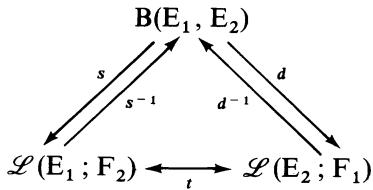
\includegraphics[keepaspectratio]{images/part001_08254dbd.jpg}}

where t is the isomorphism of transposition (II, p.~46, prop. 5 and corollary). In view of the definition of weak topologies on \(F_{1}\) and \(F_{2}\) , it is immediate that when \(\mathbf{B}(\mathbf{E}_{1}, \mathbf{E}_{2})\) , \(\mathcal{L}(\mathbf{E}_{1}; \mathbf{E}_{2})\) and \(\mathcal{L}(\mathbf{E}_{2}; \mathbf{F}_{1})\) are assigned the topology of simple convergence, the isomorphisms of diagram (3) are topological vector space isomorphisms.

\subsection{Separately continuous bilinear mappings on a product of Fréchet spaces}

PROPOSITION 2. --- Let E, F and G be three locally convex spaces. Suppose that E and F are metrizable and E is barrelled. Let H be a set of separately continuous bilinear mappings from E × F into G. Suppose that for every x ∈ E, the set of mappings u(x, .) from F into G, where u runs through H, is equicontinuous. Then H is equicontinuous.

Let \(\mathrm{U}_n(\text{resp. } \mathrm{V}_n)\) be a fundamental sequence of neighbourhoods of 0 in E (resp. F). If H is not equicontinuous, there exists a closed, convex, balanced neighbourhood W of 0 in G such that for all \(n\) , \(\mathrm{H}(\mathrm{U}_n \times \mathrm{V}_n)\) is not contained in W. There exists then a sequence of pairs \((x_n, y_n) \in \mathrm{U}_n \times \mathrm{V}_n\) , and a sequence \((u_n)\) of elements of H, such that \(u_n(x_n, y_n) \notin \mathrm{W}\) . Let \(p\) be the gauge of W. For every \(y \in \mathrm{F}\) and every \(u \in \mathrm{H}\) , the mapping \(u(., y)\) from E into G is continuous, hence \(p \circ u(., y)\) is a continuous seminorm on E. On the other hand, for every \(x \in \mathrm{E}\) , the set of mappings \(u(x, .)\) for \(u \in \mathrm{H}\) is equicontinuous; since the sequence \((y_n)\) tends to 0, it is bounded, and the set of all \(u(x, y_n)\) , for \(n \geqslant 0\) and \(u \in \mathrm{H}\) , is bounded (III, p.~22, prop. 9). It follows from this that the function \(p'(x) = \sup_{\substack{u \in \mathrm{H} \\ n \geqslant 0}} p(u(x, y_n))\) is a lower semi-continuous semi-

norm (finite) on E. Since E is barrelled, \(p'\) is continuous (III, p.~24, corollary). Since \((x_{n})\) tends to 0 in E, \(p'(x_{n})\) tends to 0, so that we have \(p'(x_{n}) \leqslant 1\) if n is large enough; but then \(p(u_{n}(x_{n}, y_{n})) \leqslant p'(x_{n}) \leqslant 1\) , hence \(u_{n}(x_{n}, y_{n}) \in \mathbf{W}\) , which contradicts the hypothesis on \(u_{n}, x_{n}, y_{n}\) .

COROLLARY 1. --- Let E and F be two Fréchet spaces, and G a locally convex space. Every separately continuous bilinear mapping from E × F into G is continuous.

In fact, every Fréchet space is barrelled (III, p.~25, corollary).

Let E and F be two locally convex spaces. We use \(\mathcal{B}(\mathrm{E},\mathrm{F})\) to denote the space of continuous bilinear forms on \(E \times F\) , with the topology of uniform convergence on sets of the form \(A \times B\) , where A (resp. B) is bounded in E (resp. F). The formula

\[
u (x, y) = \langle y, \phi (u) (x) \rangle
\]

(for \(x \in \mathrm{E}\) , \(y \in \mathrm{F}\) and \(u \in \mathcal{B}(\mathrm{E}, \mathrm{F})\) ) defines a continuous linear injective mapping \(\phi\) from \(\mathcal{B}(\mathrm{E}, \mathrm{F})\) into \(\mathcal{L}_b(\mathrm{E}; \mathrm{F}_b')\) .

COROLLARY 2. --- Suppose that E and F are metrizable and that E is barrelled. Then \(\phi\) is a topological vector space isomorphism from \(\mathcal{B}(\mathrm{E},\mathrm{F})\) onto \(\mathcal{L}_b(\mathrm{E};\mathrm{F}_b')\) .

Let \(f \in \mathcal{L}_b(\mathrm{E}; \mathrm{F}_b')\) . Put \(u(x, y) = \langle y, f(x) \rangle\) for \(x \in \mathrm{E}\) and \(y \in \mathrm{F}\) . The bilinear form \(u\) on \(\mathrm{E} \times \mathrm{F}\) is separately continuous; by prop. 2, it belongs to \(\mathcal{B}(\mathrm{E}, \mathrm{F})\) , and we have \(f = \phi(u)\) . Hence \(\phi\) is a linear bijection from \(\mathcal{B}(\mathrm{E}, \mathrm{F})\) onto \(\mathcal{L}_b(\mathrm{E}; \mathrm{F}_b')\) . It is immediate that \(\phi\) is bicontinuous, hence cor. 2 follows.

\subsection{Hypocontinuous bilinear mappings}

In what follows, we shall define a notion which is intermediate between that of a continuous bilinear mapping and that of a separately continuous bilinear mapping.

PROPOSITION 3. --- Let E, F, G be three locally convex spaces, S a family of bounded subsets of E. Let u be a separately continuous bilinear mapping from E × F into G. The following properties are equivalent :

\begin{enumerate}
\def\labelenumi{\alph{enumi})}
\item
  For every neighbourhood \(\mathbf{W}\) of 0 in \(\mathbf{G}\) and every set \(\mathbf{M} \in \mathfrak{S}\) , there exists a neighbourhood \(\mathbf{V}\) of 0 in \(\mathbf{F}\) such that \(u(\mathbf{M} \times \mathbf{V}) \subset \mathbf{W}\) .
\item
  For every set \(\mathbf{M} \in \mathfrak{S}\) , the image of \(\mathbf{M}\) under the mapping \(x \mapsto u(x, .)\) is an equicontinuous subset of \(\mathcal{L}(\mathrm{F}; \mathrm{G})\) .
\item
  The mapping \(y \mapsto u(., y)\) from \(\mathbf{F}\) into \(\mathcal{L}_{\mathfrak{S}}(\mathbf{E}; \mathbf{G})\) is continuous.
\item
  expresses that \(y \mapsto u(., y)\) is continuous at the point 0, on account of the definition of neighbourhoods of 0 in \(\mathcal{L}_{\mathfrak{S}}(\mathrm{E}; \mathrm{G})\) (III, p.~13); likewise a) expresses that the image of M under the mapping \(x \mapsto u(x, .)\) is equicontinuous at the point 0 (III, p.~16).
\end{enumerate}

DEFINITION 2. --- Let u be a bilinear mapping from E × F into G. We say that u is S-hypocontinuous if u is separately continuous and if it verifies one of the equivalent conditions a), b), c) of prop. 3.

The condition \(c)\) of prop. 3 shows that the notion of \(\mathfrak{S}\) -hypocontinuous bilinear mapping depends on \(\mathfrak{S}\) only through the \(\mathfrak{S}\) -topology on \(\mathcal{L}(\mathrm{E},\mathrm{G})\) .

For every set T of bounded subsets of F, we define similarly the notion of T-hypo-continuous mapping, by interchanging the roles of E and F in prop. 3. A separately continuous bilinear mapping u is said to be \((\mathfrak{S}, \mathfrak{T})\) -hypocontinuous if it is both S-hypocontinuous and T-hypocontinuous.

Every continuous bilinear mapping from \(E \times F\) into G is \((\mathfrak{S}, \mathfrak{T})\) -hypocontinuous for every pair \((\mathfrak{S}, \mathfrak{T})\) of sets of bounded subsets: for every neighbourhood W of 0 in G, there exists a neighbourhood U of 0 in E and a neighbourhood V of 0 in F such that \(u(U \times V) \subset W\) ; since every set \(M \in S\) is bounded, there exists \(\lambda > 0\) such that \(\lambda M \subset V\) , and so

\[
u (\mathbf {M} \times \lambda \mathbf {V}) = u (\lambda \mathbf {M} \times \mathbf {V}) \subset u (\mathbf {U} \times \mathbf {V}) \subset \mathbf {W}.
\]

The converse is in general false (III, p.~47, exerc. 3).

PROPOSITION 4. --- Let u be a S-hypocontinuous bilinear mapping from E × F into G. For every set M ∈ S, the restriction of u to M × F is continuous, and u(M × Q) is bounded in G for every bounded subset Q of F.

The first assertion follows from cor. 3 of GT, X, § 2, No.~1. Let W be a neighbourhood of 0 in G; there exists, by hypothesis, a neighbourhood V of 0 in F such that \(u(\mathbf{M} \times \mathbf{V}) \subset \mathbf{W}\) . Since there exists \(\lambda \neq 0\) such that \(\lambda \mathbf{Q} \subset \mathbf{V}\) , we have \(\lambda u(\mathbf{M} \times \mathbf{Q}) = u(\mathbf{M} \times \lambda \mathbf{Q}) \subset \mathbf{W}\) , and this proves the second part of the proposition.

PROPOSITION 5. --- Let u be a (S, T)-hypocontinuous bilinear mapping from E × F into G. For every pair of sets M ∈ S, N ∈ T, u is uniformly continuous on M × N. The proposition follows immediately from prop. 2 of GT, X, § 2, No.~1 and prop. 5 of GT, X, § 2, No.~2.

PROPOSITION 6. --- If F is a barrelled space, every separately continuous bilinear mapping u from E × F into a locally convex space G is S-hypocontinuous for every set S of bounded subsets of E.

In other words, the linear mapping \(y \mapsto u(., y)\) from \(F\) into \(\mathcal{L}_b(E; G)\) is continuous. It is enough (III, p.~30, prop. 3) to prove that the image of every bounded subset \(M\) of \(E\) under \(x \mapsto u(x, .)\) is equicontinuous in \(\mathcal{L}(F; G)\) . But, by virtue of prop. 1 (III, p.~28) this image is a simply bounded subset of \(\mathcal{L}(F; G)\) , and since \(F\) is barrelled, every simply bounded subset of \(\mathcal{L}(F; G)\) is equicontinuous (III, p.~25, th. 1).

Remark. --- Suppose the topology of F is the finest locally convex topology on F for which the linear mappings \(h_{\alpha}:F_{\alpha}\to F\) are continuous (II, p.~27). Then condition c) of prop. 3 (III, p.~30) shows that if E and G are locally convex, then the bilinear mapping \(u:E\times F\to G\) is S-hypocontinuous if and only if each of the bilinear mappings

\[
(x, y _ {\alpha}) \mapsto u (x, h _ {\alpha} (y _ {\alpha}))
\]

from \(\mathbf{E} \times \mathbf{F}_{\alpha}\) into \(\mathbf{G}\) is \(\mathfrak{S}\) -hypocontinuous.

Now suppose that \(\mathbf{E}\) is a locally convex space which is the strict inductive limit of an increasing sequence \((\mathbf{E}_n)\) of closed vector subspaces of \(\mathbf{E}\) (II, p.~33); then every set \(\mathbf{M} \in \mathfrak{S}\) is contained in one of the \(\mathbf{E}_n\) and is bounded in this subspace (III, p.~5, prop. 6). We denote by \(\mathfrak{S}_n\) the family of all subsets belonging to \(\mathfrak{S}\) contained in \(\mathbf{E}_n\) .

Condition a) of prop. 3 (III, p.~30) shows that for a bilinear mapping \(u: \mathrm{E} \times \mathrm{F} \to \mathrm{G}\) to be \(\mathfrak{S}\) -hypocontinuous, it is necessary and sufficient that each of the restrictions \(u_n: \mathrm{E}_n \times \mathrm{F} \to \mathrm{G}\) of \(u\) is \(\mathfrak{S}_n\) -hypocontinuous.

\subsection{Extension of a hypocontinuous bilinear mapping}

PROPOSITION 7. --- Let E, F, G be three locally convex spaces, G being assumed Hausdorff; let \(E_{0}\) (resp. \(F_{0}\) ) be a dense vector subspace of E (resp. F). Let u be a separately continuous bilinear mapping from \(E \times F\) into G.

\begin{enumerate}
\def\labelenumi{\arabic{enumi})}
\item
  If \(u(\mathrm{E}_0 \times \mathrm{F}_0) = \{0\}\) , then \(u = 0\) .
\item
  Let \(\mathfrak{S}_0\) be a family of bounded subsets of \(\mathbf{E}_0\) ; if the restriction of \(u\) to \(\mathbf{E}_0 \times \mathbf{F}_0\) is \(\mathfrak{S}_0\) -hypocontinuous then so is \(u\) .
\item
  By hypothesis, for all \(x \in \mathrm{E}_0\) , the continuous linear mapping \(u(x, .)\) is null on \(\mathrm{F}_0\) , hence on \(\mathrm{F}\) : therefore for all \(y \in \mathrm{F}\) , the continuous linear mapping \(u(., y)\) is null on \(\mathrm{E}_0\) , hence on \(\mathrm{E}\) . This proves that \(u = 0\) .
\item
  For every closed neighbourhood W of 0 in G and for every set \(\mathbf{M} \in \mathfrak{S}_0\) , there exists, by hypothesis, a neighbourhood V of 0 in \(\mathrm{F}_0\) such that \(u(\mathbf{M} \times \mathbf{V}) \subset \mathbf{W}\) . But \(\overline{\mathbf{V}}\) is a neighbourhood of 0 in F; for every \(x \in \mathbf{M}\) , the relation \(u(\{x\} \times \mathbf{V}) \subset \mathbf{W}\) implies that \(u(\{x\} \times \overline{\mathbf{V}}) \subset \mathbf{W}\) , since \(u(x, .)\) is continuous and W is closed; therefore \(u(\mathbf{M} \times \overline{\mathbf{V}}) \subset \mathbf{W}\) , which proves that \(u\) is \(\mathfrak{S}_0\) -hypocontinuous.
\end{enumerate}

PROPOSITION 8. --- Let E, F, G be three locally convex spaces; assume that G is Hausdorff and quasi-complete. Let \(E_{0}\) (resp. \(F_{0}\) ) be a dense vector subspace of E (resp. F), \(S_{0}\) (resp. \(T_{0}\) ) a family of bounded subsets of \(E_{0}\) (resp. \(F_{0}\) ) such that every point of E (resp. F) is in the closure of an element of \(S_{0}\) (resp. \(T_{0}\) ). Then every \((\mathfrak{S}_{0}, \mathfrak{T}_{0})\) -hypocontinuous bilinear mapping u from \(E_{0} \times F_{0}\) into G extends uniquely to a separately continuous bilinear mapping \(\overline{u}\) from E × F into G and \(\overline{u}\) is \((\mathfrak{S}_{0}, \mathfrak{T}_{0})\) -hypocontinuous.

The uniqueness and hypocontinuity of \(\overline{u}\) follows from prop. 7; it remains to prove the existence of \(\overline{u}\) . For every \(y' \in F_{0}\) , the continuous linear mapping \(x' \mapsto u(x', y')\) from \(E_{0}\) into G extends uniquely to a continuous linear mapping \(x \mapsto u_{1}(x, y')\) from E into G (III, p.~8, prop. 10). It follows immediately that for every \(x \in E\) , the mapping \(y' \mapsto u_{1}(x, y')\) from \(F_{0}\) into G is linear; and we shall show that it is continuous. By hypothesis, there exists \(M \in S_{0}\) , such that \(x \in M\) . For every closed neighbourhood W of 0 in G, there exists, by hypothesis, a neighbourhood V of 0 in \(F_{0}\) such that \(u(M \times V) \subset W\) ; since \(x \mapsto u_{1}(x, y')\) is continuous, we deduce that \(u_{1}(\overline{\mathbf{M}} \times \mathbf{V}) \subset \mathbf{W}\) , and in particular \(u_{1}(x, y') \in \mathbf{W}\) for all \(y' \in V\) . This establishes our assertion. By virtue of prop. 7, the bilinear map \(u_{1}\) from \(E \times F_{0}\) into G is \((\mathfrak{S}_{0}, \mathfrak{T}_{0})\) -hypocontinuous. We end the proof by interchanging the roles of E and F in the first part of the proof, applied to \(u_{1}\) .

\subsection{\texorpdfstring{Hypocontinuity of the mapping \((u, v) \mapsto v \circ u\)}{Hypocontinuity of the mapping (u, v) \textbackslash mapsto v \textbackslash circ u}}

PROPOSITION 9. --- Let R, S, T be three locally convex Hausdorff spaces. Suppose that the spaces \(\mathcal{L}(\mathbf{R};\mathbf{S})\) , \(\mathcal{L}(\mathbf{S};\mathbf{T})\) , \(\mathcal{L}(\mathbf{R};\mathbf{T})\) are each assigned the topology of simple (resp. compact, bounded) convergence. Then the bilinear mapping \((u, v) \mapsto v \circ u\) from \(\mathcal{L}(\mathrm{R}; \mathrm{S}) \times \mathcal{L}(\mathrm{S}; \mathrm{T})\) into \(\mathcal{L}(\mathrm{R}; \mathrm{T})\) is \((\mathfrak{S}, \mathfrak{T})\) -hypocontinuous, where \(\mathfrak{T}\) is the family of equicontinuous subsets of \(\mathcal{L}(\mathrm{S}; \mathrm{T})\) , and \(\mathfrak{S}\) the family of finite (resp. compact, bounded) subsets of \(\mathcal{L}(\mathrm{R}; \mathrm{S})\) .

We first prove that \((u, v) \mapsto v \circ u\) is \(\mathfrak{T}\) -hypocontinuous. Let H be an equicontinuous set in \(\mathcal{L}(S; T)\) , let W be a neighbourhood of 0 in T and let M be a finite (resp. compact, bounded) subset of R. We must show that there exists a neighbourhood V of 0 in S such that if \(u(M) \subset V\) and \(v \in H\) , then \(v(u(M)) \subset W\) . But for this, it is enough to have \(v(V) \subset W\) for all \(v \in H\) , and the existence of such a neighbourhood follows from the equicontinuity of H.

To see that \((u, v) \mapsto v \circ u\) is \(\mathfrak{S}\) -hypocontinuous, we shall prove that, for every neighbourhood \(W\) of 0 in \(T\) , every finite (resp. compact, bounded) subset \(M\) of \(R\) and every finite (resp. compact, bounded) subset \(L\) of \(\mathcal{L}(R; S)\) there exists a finite (resp. compact, bounded) subset \(N\) of \(S\) such that the relations \(v(N) \subset W\) and \(u \in L\) imply that \(v(u(M)) \subset W\) . Evidently it is enough to show that we can take \(N = \bigcup_{u \in L} u(M)\) ,

i.e.~that the set N is finite (resp. compact, bounded) whenever L and M are. This is immediate if L and M are finite, or if M is bounded in R and L is bounded in \(\mathcal{L}(\mathrm{R};\mathrm{S})\) (for the topology of bounded convergence, cf.~III, p.~22). Finally, we show that if M is compact in R and L is compact in \(\mathcal{L}(\mathrm{R};\mathrm{S})\) for the topology of compact convergence, then N is compact in S. But if \(u_{M}\) is the restriction to M of \(u \in L\) , the mapping \(u \mapsto u_{M}\) from L into the space \(\mathcal{C}(\mathrm{M};\mathrm{S})\) of all continuous mappings from M into S, with the topology of uniform convergence, is continuous; hence the image of L under this mapping is compact, and our assertion then follows from the continuity of the map \((w,x) \mapsto w(x)\) from \(\mathcal{C}(\mathrm{M};\mathrm{S}) \times \mathrm{M}\) into S (GT, X, § 1, No.~6, prop. 9).

In the two corollaries that follow, we assume as in prop. 9, that the spaces \(\mathcal{L}(\mathbf{R};\mathbf{S})\) , \(\mathcal{L}(\mathbf{S};\mathbf{T})\) , \(\mathcal{L}(\mathbf{R};\mathbf{T})\) are all three assigned the topology of simple convergence, or all three the topology of compact convergence, or all three that of bounded convergence.

COROLLARY 1. --- For every equicontinuous subset H of \(\mathcal{L}(\mathbf{S};\mathbf{T})\) the map \((u,v)\mapsto v\circ u\) from \(\mathcal{L}(\mathbf{R};\mathbf{S})\times \mathbf{H}\) into \(\mathcal{L}(\mathbf{R};\mathbf{T})\) is continuous.

This follows immediately from prop. 9 (III, p.~32) and 4 (III, p.~31).

COROLLARY 2. --- Suppose S is barrelled. If the sequence \((u_n)\) tends to \(u\) in \(\mathcal{L}(\mathbf{R};\mathbf{S})\) and the sequence \((v_{n})\) to \(v\) in \(\mathcal{L}(\mathbf{S},\mathbf{T})\) , then the sequence \((v_{n}\circ u_{n})\) tends to \(v\circ u\) in \(\mathcal{L}(\mathbf{R};\mathbf{T})\) .

In fact, the sequence \((v_{n})\) , being simply bounded in \(\mathcal{L}(\mathrm{S};\mathrm{T})\) is equicontinuous, since \(\mathrm{S}\) is barrelled (III, p.~25, th. 1); the corollary is then a consequence of cor. 1.

\section{BOREL'S GRAPH THEOREM}

\subsection{Borel's graph theorem}

THEOREM 1. --- Let E be a locally convex space which is the inductive limit of Banach spaces, F a Souslin locally convex space, for example a Lusin space (GT, IX, § 6, No.~2 and No.~4), and u a linear mapping from E into F. If the graph of u is a Borel subset of E × F, then u is continuous.

Let \(E_i\) be a family of Banach spaces, and \((u_i)\) a family of continuous linear mappings \(u_i: E_i \to E\) such that the topology of \(E\) is the finest locally convex topology for which the \(u_i\) are continuous. It is enough to prove that the composed mappings \(u \circ u_i\) are continuous, or in fact (GT, IX, § 2, No.~6, prop. 10) that the restriction of \(u \circ u_i\) to every closed subspace \(G\) of \(E_i\) satisfying the first axiom of countability is continuous. The graph of this restriction is the inverse image of the graph of \(u\) under the continuous mapping \(u_i \times \text{Id}_F: G \times F \to E \times F\) , hence is a Borel set in \(G \times F\) . In addition, \(G \times F\) is a Souslin space and every Borel subset of a Souslin space is a Souslin space (GT, IX, § 6, No.~3, prop. 10). Th. 1 then follows from th. 4, GT, IX, § 6, No.~8.

Remark. --- Recall (III, p.~12) that every homological Hausdorff and semi-complete space, for example every Fréchet space, is the inductive limit of Banach spaces. * This is also true for the strong dual of a reflexive Fréchet space (IV, p.~23, prop. 4). *

\subsection{Locally convex Lusin spaces}

PROPOSITION 1. --- Let E be a Hausdorff locally convex space. Suppose that there exists a sequence \((\mathrm{E}_{n})_{n\in\mathbb{N}}\) of Fréchet spaces satisfying the first axiom of countability, and continuous linear mappings \(u_{n}:E_{n}\to E\) such that \(\mathrm{E}=\bigcup_{n\in\mathbb{N}}u_{n}(\mathrm{E}_{n})\) . Then E is a Lusin space.

Let \(P_n\) be the kernel of \(u_n\) ; then \(u_n\) defines a bijective continuous mapping from the quotient space \(E_n / P_n\) onto \(u_n(E_n)\) . Since \(E_n / P_n\) is a Fréchet space satisfying the first axiom of countability (GT, IX, § 3, No.~1), hence a polish space (GT, IX, § 6, No.~1, def. 1), \(u_n(E_n)\) is a Lusin subspace of E (GT, IX, § 6, No.~4, prop. 11). Therefore by GT, IX, § 6, No.~7, cor. of th. 3, the space E, which is regular (GT, III, § 3, No.~1) is a Lusin space.

Example 1. --- Every Fréchet space satisfying the first axiom of countability is a polish space, hence a Lusin space. Consequently, so are the spaces \(\mathcal{C}(\mathrm{X})\) , where \(\mathrm{X}\) is locally compact and has a countable base (the topology of \(\mathcal{C}(\mathrm{X})\) being that of compact convergence, cf.~GT, X, § 3, No.~3, corollary and § 1, No.~6, cor. 3); * the spaces \(\mathcal{C}^{\infty}(\mathrm{U})\) , where U is an open subset of \(\mathbf{R}^{n}\) (III, p.~9) and \(\mathcal{H}(\mathrm{U})\) , where U is an open subset of \(\mathbf{C}^{n}\) (III, p.~10).

Prop. 1 shows that the spaces \(\mathcal{C}_0^\infty (\mathbf{U})\) , where \(\mathbf{U}\) is an open set in \(\mathbf{R}^n\) , \(\mathcal{G}_s(\mathbf{I})\) , where \(\mathbf{I}\) is a compact interval in \(\mathbf{R}\) and \(s\geqslant 1\) , and \(\mathcal{H}(\mathbf{K})\) , where \(\mathbf{K}\) is a compact subset of \(\mathbf{C}^n\) are all Lusin spaces (III, p.~10).

THEOREM 2. --- Let E be a locally convex space, which is the inductive limit of an increasing sequence \((\mathrm{E}_n)_{n\in \mathbb{N}}\) of subspaces of E, endowed with the topologies of Fréchet spaces satisfying the first axiom of countability. Suppose that every compact subset of E is contained in one of the \(E_{n}\) and is compact in this space. Let F be a Fréchet space satisfying the first axiom of countability. Then the space \(\mathcal{L}_{c}(E;F)\) is a Lusin space.

The space E is bornological (III, p.~12), hence the space \(\mathcal{L}_c(\mathrm{E};\mathrm{F})\) is complete (III, p.~23, prop. 12). The linear mapping \(j\colon f\mapsto (f|\mathrm{E}_n)_{n\in \mathbf{N}}\) is an injection from \(\mathcal{L}_c(\mathrm{E};\mathrm{F})\) into the product space \(\prod_{n\in \mathbf{N}}\mathcal{L}_c(\mathrm{E}_n;\mathrm{F})\) ; by virtue of the hypothesis on the compact subsets of E and the definition of the \(\mathfrak{S}\) -topologies, \(j\) is an isomorphism from \(\mathcal{L}_c(\mathrm{E};\mathrm{F})\) onto its image (endowed with the topology induced by the product topology); moreover, since \(\mathcal{L}_c(\mathrm{E};\mathrm{F})\) is complete, this image is a closed subspace of \(\prod_{n\in \mathbf{N}}\mathcal{L}_c(\mathrm{E}_n;\mathrm{F})\)

(GT, II, § 3, No.~4, prop. 8). By GT, IX, § 6, No.~4, it is therefore enough to prove that each of the spaces \(\mathcal{L}_c(\mathrm{E};\mathrm{F})\) is a Lusin space. For the rest of the proof, we shall assume that E is a Fréchet space satisfying the first axiom of countability.

Since F is a Fréchet space satisfying the first axiom of countability, it is isomorphic to a closed subspace of a countable product of Banach spaces \(F_{n}\) , each of which is a quotient of F (II, p.~5), hence satisfies the first axiom of countability. The linear mapping \(j': f \mapsto (\mathrm{pr}_{n} \circ f)_{n \in \mathbb{N}}\) is an injection from \(\mathcal{L}_{c}(\mathrm{E}; \mathrm{F})\) into the product space \(\prod_{n \in \mathbb{N}} \mathcal{L}_{c}(\mathrm{E}; \mathrm{F}_{n})\) , and by using the definition of the S-topologies and of the open sets in a product, \(j'\) is an isomorphism from \(\mathcal{L}_{c}(\mathrm{E}; \mathrm{F})\) onto its image; moreover, since \(\mathcal{L}_{c}(\mathrm{E}; \mathrm{F})\) is complete, this image is a closed subspace of \(\prod_{n \in \mathbb{N}} \mathcal{L}_{c}(\mathrm{E}; \mathrm{F})\) . Therefore it is enough to prove that each of the spaces \(\mathcal{L}_{c}(\mathrm{E}; \mathrm{F}_{n})\) is a Lusin space (GT, IX, § 6, No.~4), and consequently, we can assume that F is a Banach space satisfying the first axiom of countability.

The space \(\mathcal{L}_{c}(\mathrm{E};\mathrm{F})\) is the union of a countable family of equicontinuous and closed subsets (III, p.~19, cor. 1 and GT, X, § 2, No.~3, prop. 6). But every equicontinuous subset H of \(\mathcal{L}_{c}(\mathrm{E};\mathrm{F})\) is metrizable and satisfies the first axiom of countability (III, p.~18, prop. 6 and GT, X, § 2, No.~4, th. 1); if H is closed, then it is a complete space for the uniform structure induced by that of \(\mathcal{L}_{c}(\mathrm{E};\mathrm{F})\) , since the latter is complete In other words, H is a polish space, and a fortiori a Lusin space; consequently the regular space \(\mathcal{L}_{c}(\mathrm{E};\mathrm{F})\) is a Lusin space (GT, IX, § 6, No.~7, cor. of th. 3).

COROLLARY. --- The hypotheses on E being as in th. 2, assume, in addition that every bounded subset of E is relatively compact. Then the strong dual of E is a Lusin space. * In particular, the strong dual of a Fréchet space satisfying the first axiom of countability, which is also a Montel space, is a Lusin space. *

* Example 2. --- Let U be an open subset of \(\mathbf{R}^{n}\) . The corollary applies in particular to the Fréchet space \(E = \mathcal{C}^{\infty}(\mathrm{U})\) ; its dual \(\mathcal{C}_{0}^{-\infty}(\mathrm{U})\) (the space of distributions with compact support on U) is then a Lusin space. The space \(\mathcal{C}_{0}^{\infty}(\mathrm{U})\) is a strict inductive limit of a sequence of Fréchet spaces \(\mathcal{C}_{K_n}^{\infty}(\mathrm{U})\) satisfying the first axiom of countability (III, p.~9). We can show that each of the spaces \(\mathcal{C}_{K_n}^{\infty}(\mathrm{U})\) is a Montel space; in addition, every bounded subset of \(\mathcal{C}_{0}^{\infty}(\mathrm{U})\) is contained in one of the spaces \(\mathcal{C}_{K_n}^{\infty}(\mathrm{U})\) (III, p.~5, prop. 6). We can then apply the corollary of th. 2. Then the dual \(\mathcal{C}_{0}^{-\infty}(\mathrm{U})\) of \(\mathcal{C}_{0}^{\infty}(\mathrm{U})\) (the space of distributions on U) is a Lusin space for the strong topology. *

Similarly we prove that for every open subset U of \(C^{n}\) , and for every compact subset K of \(C^{n}\) , the strong dual of \(\mathcal{H}(U)\) and the strong dual of \(\mathcal{H}(K)\) are Lusin spaces. *

Remark. --- Let E be as in th. 2; let F be a Hausdorff locally convex space which is the union of the images of a sequence of continuous linear mappings \(u_n: \mathrm{F}_n \to \mathrm{F}\) , where each \(\mathrm{F}_n\) is a Fréchet space satisfying the first axiom of countability; then \(\mathcal{L}_c(\mathrm{E};\mathrm{F})\) is a Lusin space. As in prop. 1, we first reduce to the case where each \(u_n\) is injective; then, as in the proof of th. 2, we can assume that E is a Fréchet space satisfying the first axiom of countability. Then, by I, p.~20, prop. 1, \(\mathcal{L}(\mathrm{E};\mathrm{F})\) is the union of the \(\mathcal{L}(\mathrm{E};\mathrm{F}_n)\) ; moreover, the canonical injection \(\mathcal{L}_c(\mathrm{E};\mathrm{F}_n) \to \mathcal{L}_c(\mathrm{E};\mathrm{F})\) is continuous (GT, X, § 1, No.~4, prop. 3). Since each of the spaces \(\mathcal{L}_c(\mathrm{E};\mathrm{F}_n)\) is a Lusin space by th. 2, \(\mathcal{L}(\mathrm{E};\mathrm{F}_n)\) is also a Lusin space for the topology induced by that of \(\mathcal{L}_c(\mathrm{E};\mathrm{F})\) (GT, IX, § 6, No.~4, prop. 11); consequently \(\mathcal{L}_c(\mathrm{E};\mathrm{F})\) is a Lusin space by virtue of GT, IX, § 6, No.~7, corollary of th. 3.

\subsection{\texorpdfstring{* Measurable linear mappings on a Banach space \(^{1}\)}{Measurable linear mappings on a Banach space \^{}\{1\}}}

PROPOSITION 2. --- Let E be a Banach space, F a locally convex space and u a linear mapping from E into F. Assume that for every closed subset B of F, every compact subset X of E and every measure \(\mu\) on X, the intersection \(X \cap u^{-1}(B)\) is \(\mu\) -measurable. Then u is continuous.

First assume that F is the base field. For every compact subset X of E and every measure \(\mu\) on X, the restriction of u to X is \(\mu\) -measurable (INT, IV). Suppose that u is not continuous. Then we can find a sequence of points \((x_{n})\) in E such that \(\sum_{n} \|x_{n}\| < \infty\) and \(|u(x_{n})| \geqslant n\) for every integer n.~Consider the mapping \(g:(t_{n}) \mapsto \sum_{n} t_{n} x_{n}\) from the cube \(C = [0, 1]^{N}\) into E; it is clear that g is continuous. Hence \(f = u \circ g\) is measurable for every measure on C (INT, V); in particular for the measure \(\mu\) which is the product of Lebesgue measures on the factors of C. Hence there exists a compact subset D of C such that \(\mu(D) > \frac{1}{2}\) and such that the restriction of f to D is continuous, hence also bounded. Let M be the upper bound of \(|f|\) on D and let \(p \in N\) be such that \(p \geqslant 4M\) . Let \(s = (s_{n})\) and \(t = (t_{n})\) be two points of D such that \(s_{n} = t_{n}\) for all \(n \neq p\) . Then

\[
f (s) - f (t) = u (\sum_ {n} s _ {n} x _ {n} - \sum_ {n} t _ {n} x _ {n}) = (s _ {p} - t _ {p}) u (x _ {p}).
\]

Since \(|f(s) - f(t)| \leqslant 2\mathbf{M}\) and \(|u(x_p)| \geqslant p \leqslant 4\mathbf{M}\) , we get

\[
\left| s _ {p} - t _ {p} \right| \leqslant \frac {1}{2}.
\]

The Lebesgue-Fubini theorem (INT, V, 2nd ed., § 8, No.~3, cor. 2 of prop. 7) implies that \(\mu(D) \leqslant \frac{1}{2}\) ; this gives a contradiction. Hence \(u\) is continuous.

In the general case, for every \(v \in F'\) , the linear form \(v \circ u\) is continuous, by the preceding argument. Let \((x_{n})_{n \in \mathbb{N}}\) be a sequence of points of E tending to 0; then the sequence \((u(x_{n}))_{n \in \mathbb{N}}\) tends to 0 in F, if F is assigned the topology \(\sigma(\mathrm{F}, \mathrm{F}')\) ; hence this sequence is bounded for \(\sigma(\mathrm{F}, \mathrm{F}')\) and so it is bounded in F (III, p.~27, cor. 3). Since E is bornological (III, p.~12, prop. 2); the linear mapping \(u: E \to F\) is continuous.*

1 The results of this section depend on the book of Integration.

\exercisesheading
\exercisegroup

\begin{enumerate}
\def\labelenumi{\arabic{enumi})}
\tightlist
\item
  Let \(\mathbf{E}\) be a left topological vector space over a non-discrete topological field \(\mathbf{K}\) . A subset \(\mathbf{B}\) of \(\mathbf{E}\) is said to be bounded if for every neighbourhood \(\mathbf{V}\) of 0 in \(\mathbf{E}\) there exists \(\lambda \neq 0\) in \(\mathbf{K}\) such that \(\lambda \mathbf{B} \subset \mathbf{V}\) .
\end{enumerate}

\begin{enumerate}
\def\labelenumi{\alph{enumi})}
\item
  Show that if B is bounded in E, then for every neighbourhood V of 0 in E, there exists a neighbourhood U of 0 in K such that U.B ⊂ V.
\item
  Show that the closure of a bounded set in E is bounded. The union of two bounded sets is bounded. Every precompact set in E is bounded. Extend the corollaries of III, p.~4, prop. 4 to topological vector spaces over K.
\item
  Prove that if A is a bounded set in K (considered as a vector space on the left over itself) and B is a bounded set in E, then A.B is bounded in E.
\item
  Extend prop. 3 of III, p.~4 to the case where K is a metrizable topological division ring. e) Extend the notion of a quasi-complete space and its properties to topological vector spaces.
\end{enumerate}

\begin{enumerate}
\def\labelenumi{\arabic{enumi})}
\setcounter{enumi}{1}
\tightlist
\item
  \begin{enumerate}
  \def\labelenumii{\alph{enumii})}
  \tightlist
  \item
    Let E be a left topological vector space over a non-discrete topological field K. Prove that if there exists a neighbourhood V of 0 in E which is bounded (exerc. 1), than the sets \(\lambda\) V, for \(\lambda \in \mathbf{K}\) and \(\lambda \neq 0\) , form a fundamental system of neighbourhoods of 0 in E. If K is metrizable, the Hausdorff topology associated with the topology of E (GT, III, § 2, No.~6) is metrizable. If \(\mathbf{K} = \mathbf{R}\) or \(\mathbf{K} = \mathbf{C}\) , the locally convex topology on E which is the finest of the topologies coarser than the given topology on E (II, p.~80, exerc. 23) can be defined by a single semi-norm.
  \end{enumerate}
\end{enumerate}

\begin{enumerate}
\def\labelenumi{\alph{enumi})}
\setcounter{enumi}{1}
\item
  Prove that the topology of an infinite product of locally convex Hausdorff spaces (of which none is just 0) cannot be defined by a single semi-norm.
\item
  Let E be a locally convex space whose topology is defined by an increasing sequence \((p_n)\) of semi-norms. In order that the topology of E be defined by a single semi-norm, it is necessary and sufficient that there exists an integer \(n_0\) such that for every \(n \geqslant n_0\) there exists a number \(k_n \geqslant 0\) such that \(p_n(x) \leqslant k_n p_{n_0}(x)\) for all \(x \in E\) .
\end{enumerate}

\(d\) ) Let E be the vector space over \(\mathbf{R}\) consisting of infinitely differentiable numerical functions on the interval \(\mathrm{I} = [0,1]\) . For every integer \(n\geqslant 0\) , let \(p_n(f) = \sup_{0\leqslant k\leqslant n}\left(\sup_{x\in I}|f^{(k)}(x)|\right)\) (with

\(f^{(0)} = f)\) ; show that the \(p_n\) are norms on E and that the topology defined by the sequence of norms \(p_n\) cannot be defined by a single norm.

\begin{enumerate}
\def\labelenumi{\arabic{enumi})}
\setcounter{enumi}{2}
\item
  Let E be a metrizable vector space over R, d a translation invariant distance, compatible with the topology of E. Let \(|x| = d(x, 0)\) (I, p.~16). Prove that for every integer n \textgreater{} 0, we have \(\frac{1}{n}|x| \leqslant \left|\frac{x}{n}\right|\) . Deduce from this that if B is a bounded subset of E, then \(\sup_{x \in B} |x| < +\infty\) (in other words, B is bounded for the distance d (GT, IX, § 2, No.~3)). Give an example of a metrizable vector space E and an unbounded set in E which is bounded for the distance d (exerc. 2).
\item
  Let E be a topological vector space over a non-discrete metrizable topological field K. Show that if E is a Baire space and if in E there exists a countable base for the bornology formed by bounded subsets of E (III, p.~37, exerc. 1), then there exists a neighbourhood of 0 in E which is bounded, and consequently the Hausdorff topology associated with the topology of E is metrizable (III, p.~37, exerc. 2) (compare with exerc. 6).
\item
  Let \(\mathbf{E}\) be a metrizable vector space over a non-discrete valuated field \(\mathbf{K}\) . Prove that if \((\mathbf{B}_n)\) is an arbitrary sequence of bounded subsets of \(\mathbf{E}\) (III, p.~37, exerc. 1), then there exists a sequence \((\lambda_n)\) of scalars \(\neq 0\) , such that the union of the sets \(\lambda_n\mathbf{B}_n\) is bounded.
\item
  Let \(\mathrm{E}\) be a locally convex space, which is the strict inductive limit of a strictly increasing sequence \((\mathrm{E}_n)\) of locally convex Hausdorff spaces, each \(\mathrm{E}_n\) being closed in \(\mathrm{E}_{n+1}\) (II, p.~32, prop. 9).
\end{enumerate}

\begin{enumerate}
\def\labelenumi{\alph{enumi})}
\tightlist
\item
  Prove that E is not metrizable (use III, p.~5, prop. 6 and the preceding exerc. 5).\\
\item
  In order that there exist a countable base for the canonical bornology of E, it is necessary and sufficient that the canonical bornology of each \(\mathrm{E}_n\) has a countable base in \(\mathrm{E}_n\) .
\end{enumerate}

\begin{enumerate}
\def\labelenumi{\arabic{enumi})}
\setcounter{enumi}{6}
\tightlist
\item
  \begin{enumerate}
  \def\labelenumii{\alph{enumii})}
  \tightlist
  \item
    Let E be an infinite dimensional Banach space and let S be the family of compact, convex and balanced subsets of E, which is a directed set for the relation \(\subset\) . Show that E is the inductive limit of the inductive system of the Banach spaces \(E_{A}\) , where A runs through S. (Prove by contradiction that a neighbourhood V of 0 for the inductive limit topology of the topologies of \(E_{A}\) contains a ball with center 0; for this, note that otherwise, there will exist a sequence \((x_{n})\) of points of E such that \(\|x_{n}\| \leqslant 1/n^{2}\) , and which will not belong to V.) Deduce from this that there exist bounded subsets in E which are not contained in any \(E_{A}\) for \(A \subset S\) .
  \end{enumerate}
\end{enumerate}

\begin{enumerate}
\def\labelenumi{\alph{enumi})}
\setcounter{enumi}{1}
\tightlist
\item
  Let E be an infinite dimensional Banach space. On the vector space \(\prod_{m=1}^{\infty}E_{m}\) , where \(E_{m}=E\) for each m, let \(T_{n}\) denote the topology obtained by taking the product of the Banach space topology on each \(E_{m}\) for \(m\leqslant n\) , and for m\textgreater n, the finest locally convex topology on \(E_{m}\) ; \(F_{n}\) denotes the locally convex space \(\prod_{m=1}^{\infty}E_{m}\) with the topology \(T_{n}\) . Every identity map \(F_{n}\to F_{n+1}\) is continuous; show that the inductive limit space of the inductive system \(F_{n}\) is the space F obtained by assigning to \(\prod_{m=1}^{\infty}E_{m}\) the topology which is the product of the Banach space topologies on each of the factors. Deduce from this that there are bounded subsets in F which are not bounded in any \(F_{n}\) .
\end{enumerate}

\begin{enumerate}
\def\labelenumi{\arabic{enumi})}
\setcounter{enumi}{7}
\item
  Prove that in a space which is an infinite product of topological vector spaces (over \(\mathbf{R}\) or \(\mathbf{C}\) ) none just the point 0, there does not exist a countable base for the canonical bornology (first show that it is enough to prove this for the space \(\mathbf{R}^{\mathbf{N}}\) , and then use III, p.~38, exerc. 4).
\item
  Let E be the vector space over R consisting of all regulated functions on the interval I = \{0, 1\} (FVR, I, p.~4). For every integer n \textgreater{} 0, let \(V_{n}\) be the set of all functions \(f \in E\) such that \(\int_{0}^{1} \sqrt{|f(t)|} dt \leqslant 1/n\) . Show that the sets \(V_{n}\) form a fundamental system of neighbourhoods of 0 for a metrizable topology which is compatible with the vector space structure of E and that for this topology the sets \(V_{n}\) are bounded; but the convex envelope of each \(V_{n}\) is the entire space E. (Observe that every function \(f \in E\) can be written as \(f = \frac{1}{2}(g + h)\) , where g and h belong to E, and
\end{enumerate}

\[
\int_ {0} ^ {1} \sqrt {| g (t) |} d t = \int_ {0} ^ {1} \sqrt {| h (t) |} d t = \frac {1}{\sqrt {2}} \int_ {0} ^ {1} \sqrt {| f (t) |} d t.
\]

Deduce from this that the only locally convex topology coarser than the topology of E is the coarsest topology on E.

\begin{enumerate}
\def\labelenumi{\arabic{enumi})}
\setcounter{enumi}{9}
\tightlist
\item
  Let \((\mathrm{E}_{\iota})_{\iota \in I}\) be an infinite family of Hausdorff topological vector spaces, none just the point 0, over a non-discrete topological field K. Let E be the direct sum vector space of the \(\mathbf{E}_{\iota}\) , and \(\mathcal{T}_0\) the topology on E defined in I, p.~24, exerc. 14. Then a subset B of E is bounded for \(\mathcal{T}_0\) (III, p.~37, exerc. 1) if and only if B is contained in a product subspace \(\prod_{\iota \in H} \mathbf{E}_{\iota}\) , where H is a finite
\end{enumerate}

subset of I and the projections of B on each \(E_{\iota}\) for \(\iota \in H\) are bounded. Deduce (for K = R or C) that, if each \(E_{\iota}\) is a quasi-complete space, then E with \(T_{0}\) is quasi-complete.

\begin{enumerate}
\def\labelenumi{\arabic{enumi})}
\setcounter{enumi}{10}
\tightlist
\item
  Let \(\mathbf{E}\) be a topological vector space over a field \(\mathbf{K}\) with a non discrete valuation.
\end{enumerate}

\begin{enumerate}
\def\labelenumi{\alph{enumi})}
\item
  For a balanced subset A of E to absorb every bounded subset (III, p.~37, exerc. 1) of E, it is sufficient that A absorbs the set of points of every sequence \((x_{n})\) tending to 0 in E. Then A is said to be bornivorous.
\item
  Let \(u\) be a linear mapping from \(E\) into a topological vector space \(F\) over \(K\) . The image of every bounded subset of \(E\) under \(u\) is bounded in \(F\) if and only if for every sequence \((x_{n})\) of points of \(E\) tending to 0, the sequence \((u(x_{n}))\) is bounded in \(F\) .
\item
  Suppose \(\mathbf{E}\) is metrizable. Show that every bornivorous subset of \(\mathbf{E}\) is a neighbourhood of 0 in \(\mathbf{E}\) . Deduce that if \(u\) is a linear mapping from \(\mathbf{E}\) into a topological vector space \(\mathbf{F}\) over \(\mathbf{K}\) which transforms every sequence converging to 0 in \(\mathbf{E}\) into a bounded sequence in \(\mathbf{F}\) , then \(u\) is continuous on \(\mathbf{E}\) .
\end{enumerate}

\begin{enumerate}
\def\labelenumi{\arabic{enumi})}
\setcounter{enumi}{11}
\item
  Let E be a Hausdorff topological vector space over a field K with a non-discrete valuation, and F a metrizable vector space over K. If u is a continuous linear mapping from E into F such that, for every bounded subset B of F, \(u^{-1}(\mathbf{B})\) is bounded in E, show that u is an isomorphism from E onto a subspace of F.
\item
  Let \(I\) be an infinite set, and \((E_{\iota})_{\iota\in I}\) a family of locally convex spaces, none of which is 0. Let \(f\) be a linear mapping from \(E = \prod_{\iota\in I}E_{\iota}\) into a Banach space \(F\) . Show that if the image of every bounded subset of E under f is a bounded subset of F, then there exists a finite subset H of I such that for every \(\iota \notin H\) , the restriction of f to \(E_{\iota}\) (considered as a subspace of E) is null. (Argue by contradiction that if not, we can construct a bounded sequence \((x_{n})\) in E whose image under f is unbounded in F.)
\item
  Show that if the topology of a metrizable locally convex space E cannot be defined by a single norm, then there does not exist a countable base for the canonical bornology of E (using III, p.~38, exerc. 5, show that otherwise there will exist a bounded bornivorous set (III, p.~39, exerc. 11) in E, and complete the argument using III, p.~39, exerc. 11, c)).
\item
  In a Hausdorff topological vector space E over R, let A be a compact convex set and B a closed, convex and bounded set. Show that the convex envelope C of the union \(A \cup B\) is a closed set. (Consider a point z in the closure of C, but not in A, and reduce to the case where z = 0. Observe that there exists a neighbourhood V of 0 and a number \(\alpha < 1\) such that the relations \(0 \leqslant \lambda \leqslant 1\) , \(x \in A\) , \(y \in B\) , \(\lambda x + (1 - \lambda)y \in V\) imply that \(\lambda \leqslant \alpha\) . Next, for every neighbourhood W of 0 consider the set of triplets \((\lambda, x, y)\) such that \(\lambda x + (1 - \lambda)y \in W\) , \(0 \leqslant \lambda \leqslant 1\) , \(x \in A\) , \(y \in B\) .)
\item
  Let \(\mathbf{E}\) be a locally convex metrizable space satisfying the first axiom of countability, such that its completion \(\hat{\mathbf{E}}\) is a Fréchet space which satisfies the first axiom of countability.
\end{enumerate}

Show that every bounded subset B of \(\hat{E}\) is contained in the closure of a bounded subset of \(\hat{E}\) . (Reduce to the case where B is countable, arranged as a sequence \((x_{n})\) ; on the other hand, let \((p_{n})\) be an increasing sequence of semi-norms defining the topology of \(\hat{E}\) ; for each integer n consider a sequence \((y_{nk})_{k\geqslant1}\) of points of E, which converges to \(x_{n}\) and is such that \(p_{n}(x_{n}-y_{nk})\leqslant1\) for all \(k\geqslant1\) .)

\begin{enumerate}
\def\labelenumi{\arabic{enumi})}
\setcounter{enumi}{16}
\tightlist
\item
  Let \(\mathbf{A}\) be the set of increasing mappings \(\geqslant 1\) from \(\mathbf{N}\) into \(\mathbf{N}\) ; for every \(\alpha \in \mathbf{A}\) , let \(\mathbf{B}_{\alpha}\) denote the set of all points \(z = (z_n) \in \mathbf{R}^{\mathbf{N}}\) such that \(|z_n| \leqslant \alpha(n)\) for all \(n \in \mathbf{N}\) .
\end{enumerate}

\begin{enumerate}
\def\labelenumi{\alph{enumi})}
\item
  Show that the sets \(\mathbf{B}_{\alpha}\) form a base for the bornology of all bounded subsets of the space \(\mathbf{R}^{\mathbf{N}}\) . b) For every \(\alpha \in \mathbf{A}\) , the set \(\mathbf{RB}_{\alpha}\) is a vector subspace of \(\mathbf{R}^{\mathbf{N}}\) , distinct from \(\mathbf{R}^{\mathbf{N}}\) and dense in \(\mathbf{R}^{\mathbf{N}}\) ; hence there exists a linear form \(f_{\alpha} \neq 0\) (not continuous) on \(\mathbf{R}^{\mathbf{N}}\) such that \(f_{\alpha}(z) = 0\) for all \(z \in \mathbf{B}_{\alpha}\) .
\item
  Let \(\mathbf{E}\) be the vector space consisting of all mappings \(g: \alpha \mapsto (g_n(\alpha)) \in \mathbf{R}^{\mathbf{N}}\) from \(\mathbf{A}\) into \(\mathbf{R}^{\mathbf{N}}\) such that for all \(n \in \mathbf{N}\) , the sum \(p_n(g) = \sum_{\alpha} |g_n(\alpha)|\) is finite. Show that the \(p_n\) are semi-norms
\end{enumerate}

which define the topology of a Fréchet space on E.

\(d\) ) Let \(\mathbf{H}\) be the set of all \(h\in \mathbf{E}\) such that \(h(\alpha)\in \mathbf{RB}_2\) for all \(\alpha \in \mathbf{A}\) ; show that \(\mathbf{H}\) is an everywhere dense vector subspace of \(\mathbf{E}\) (observe that every \(h\in \mathbf{E}\) such that \(h(\alpha) = 0\) except for a finite number of values of \(\alpha \in \mathbf{A}\) belongs to \(\mathbf{H}\) ).

\begin{enumerate}
\def\labelenumi{\alph{enumi})}
\setcounter{enumi}{4}
\tightlist
\item
  Let \(\mathrm{E}_0 \subset \mathrm{E}\) be the vector subspace of \(\mathrm{E}\) consisting of all \(g \in \mathrm{E}\) such that \(\sum_{\alpha} |f_{\alpha}(g(\alpha))| < +\infty\) ;
\end{enumerate}

the mapping \(u: g \mapsto (f_{\alpha}(g(\alpha)))_{\alpha \in \mathbf{A}}\) is then a linear mapping from \(\mathrm{E}_0\) into the Banach space \(\mathrm{F} = \ell^1(\mathrm{A})\) (I, p.~4). Prove that \(u(\mathrm{E}_0)\) is everywhere dense in \(\mathrm{F}\) (observe that for every finite subset \(\mathrm{J}\) of \(\mathrm{A}\) , there exists \(g \in \mathrm{E}_0\) such that \(g(\alpha) = 0\) for all \(\alpha \in \mathrm{A} - \mathrm{J}\) and that the \(f_{\alpha}(g(\alpha))\) for \(\alpha \in \mathrm{J}\) take arbitrary values in \(\mathbf{R}\) ). Show that \(u^{-1}(0)\) is everywhere dense in \(\mathrm{E}_0\) (use \(d\) ). Finally, show that for every bounded subset \(C\) of \(E\) , there exists \(\alpha_0 \in A\) such that \(f_{\alpha_0}(g(\alpha_0)) = 0\) for all \(g \in C \cap E_0\) , and deduce that the closure of \(u(C \cap E_0)\) in \(F\) is not a neighbourhood of 0 in \(F\) .

\begin{enumerate}
\def\labelenumi{\alph{enumi})}
\setcounter{enumi}{5}
\tightlist
\item
  Let G be the graph of u in \(E_{0} \times F\) , a vector subspace of the Fréchet space \(E \times F\) . Show that G is everywhere dense in \(E \times F\) (observe that for every \(x \in E_{0}\) , \(x + u^{-1}(0)\) is dense in E). However, show that for every bounded subset M of G, the closure \(\overline{M}\) of M in \(E \times F\) does not contain the bounded set \(\{0\} \times U\) of \(E \times F\) , where U is the unit ball in F (if \(N = \text{pr}_{1}(M)\) , observe that because of e), \(\overline{u(N)}\) cannot contain U).
\end{enumerate}

\begin{enumerate}
\def\labelenumi{\arabic{enumi})}
\setcounter{enumi}{17}
\tightlist
\item
  In the Banach space \(\ell^1 (\mathbf{N})\) (I, p.~4) let \(e_m\) be the sequence \((\delta_{mn})_{n\geq 0}\) such that \(\delta_{mn} = 0\) for \(m\neq n\) and \(\delta_{nn} = 1\) . Define a continuous mapping from \(\ell^1 (\mathbf{N})\) in \(\mathbf{R}\) which transforms the bounded sequence of the \(e_n\) into a non bounded subset of \(\mathbf{R}\) (use Urysohn's th. (GT, IX, §4, No.~2, th. 2)).
\end{enumerate}

\exercisegroup

\begin{enumerate}
\def\labelenumi{\arabic{enumi})}
\tightlist
\item
  Let E be a locally convex space, and T its topology. Amongst the locally convex topologies on E for which the bounded sets are the same as those for T, there is one \(T'\) finer than all the others, and this is the only one amongst these topologies which is bornological. The space obtained by assigning E with \(T'\) is called the bornological space associated with E. A linear map u from E into a locally convex space F transforms every bounded subset of E into a bounded subset of F if and only if it is continuous for the topology \(T'\) .
\end{enumerate}

Show that the topology \(\mathcal{T}'\) is the finest of the locally convex topologies on \(E\) for which the canonical injections \(E_A \to E\) , where \(A\) runs through the family of convex, bounded and balanced subsets of \(E\) , are continuous.

\begin{enumerate}
\def\labelenumi{\arabic{enumi})}
\setcounter{enumi}{1}
\tightlist
\item
  Let I be an infinite set and \((\mathrm{E}_{\iota})_{\iota \in \mathrm{I}}\) a family of locally convex spaces, none of which is 0. a) Suppose that each space \(\mathrm{E}_{\iota}\) is bornological. Show that if, in addition, the product space \(\mathbf{R}^{\mathrm{I}}\) is bornological, then the product \(\mathrm{E} = \prod_{\iota \in \mathrm{I}}\mathrm{E}_{\iota}\) is bornological (using III, p.~11, prop. 1 (iii)
\end{enumerate}

and p.~39, exerc. 15, reduce to proving the following: a linear mapping \(f\) from \(E\) into a Banach space, which transforms every bounded set into a bounded set, and whose restriction to each \(E_{\iota}\) is null, is necessarily null on \(E\) . For this consider, for every \(x = (x_{\iota}) \in E\) , the restriction of \(f\) to the product of lines \(\mathbf{R}x_{\iota}\) .

\begin{enumerate}
\def\labelenumi{\alph{enumi})}
\setcounter{enumi}{1}
\tightlist
\item
  Deduce from \(a\) ) that every product of a sequence \((\mathrm{E}_n)\) of bornological spaces is bornological.
\end{enumerate}

\begin{enumerate}
\def\labelenumi{\arabic{enumi})}
\setcounter{enumi}{2}
\tightlist
\item
  Let \(\mathbf{E}\) be a locally convex space, \(\mathbf{L}\) a vector subspace of \(\mathbf{E}\) of finite codimension, and \(\mathbf{S}\) a convex balanced bornivorous set (III, p.~39, exerc. 11) in \(\mathbf{L}\) . We shall prove that there exists a convex, balanced and bornivorous set \(\mathbf{S}'\) in \(\mathbf{E}\) such that \(\mathbf{S} = \mathbf{S}' \cap \mathbf{L}\) .
\end{enumerate}

\begin{enumerate}
\def\labelenumi{\alph{enumi})}
\item
  We can reduce to the case where L is a hyperplane such that \(E = L \oplus Ra\) for a point \(a \notin L\) , and such that there exists a bounded sequence \((x_{n})\) in E such that if we put \(x_{n} = \lambda_{n}(y_{n} + a)\) with \(\lambda_{n} \in R\) and \(y_{n} \in L\) , then \(|\lambda_{n}|\) tends to \(+\infty\) ; if \(B_{0}\) is the convex balanced envelope of the set consisting of a and the \(x_{n}\) , then we have \(y_{n} + a \in \lambda_{n}^{-1}B_{0}\) for all n.
\item
  Let \(\mathfrak{B}\) be the set of all bounded, convex, balanced subsets of \(E\) which contain \(\mathbf{B}_0\) ; by hypothesis, for every \(\mathbf{B} \in \mathfrak{B}\) , there exists \(\rho_{\mathbf{B}} > 0\) such that \(2\rho_{\mathbf{B}}\mathbf{B} \cap \mathbf{L} \subset \mathbf{S}\) . Show that if \(\mathbf{R}\) is the convex balanced envelope of the union of the sets \(\rho_{\mathbf{B}}\mathbf{B}\) for \(\mathbf{B} \in \mathfrak{B}\) , then we have \(\mathbf{R} \cap \mathbf{L} \subset \mathbf{S}\) .
\end{enumerate}

\begin{enumerate}
\def\labelenumi{\arabic{enumi})}
\setcounter{enumi}{3}
\tightlist
\item
  Deduce from exerc. 3 that if E is a locally convex bornological space, then every subspace of E with finite codimension is bornological (cf.~IV, p.~64, exerc. 11).
\end{enumerate}

\exercisegroup

\begin{enumerate}
\def\labelenumi{\arabic{enumi})}
\item
  Let X be a Hausdorff topological space, and F a topological vector space (over R or C). Show that on the space \(\mathcal{C}(X; F)\) of all continuous maps from X into F, the topology of compact convergence is compatible with the vector space structure.
\item
  Let \(\mathbf{E}\) and \(\mathbf{F}\) be two Hausdorff locally convex spaces, and \(\mathfrak{S}\) a family of bounded subsets of \(\mathbf{E}\) .
\end{enumerate}

\begin{enumerate}
\def\labelenumi{\alph{enumi})}
\item
  Show that if F is not just 0, then a necessary (and sufficient) condition for \(\mathcal{L}_{\mathfrak{S}}(\mathrm{E};\mathrm{F})\) to be Hausdorff is that the union of the sets of S is total in E (use Hahn-Banach th.).
\item
  Suppose that \(\mathfrak{S}\) is a cover for E. Show that there exists an isomorphism from F onto a closed subspace of \(\mathcal{L}_{\mathfrak{S}}(\mathrm{E};\mathrm{F})\) . Deduce that if \(\mathcal{L}_{\mathfrak{S}}(\mathrm{E};\mathrm{F})\) is quasi-complete, then F is necessarily quasi-complete.
\item
  Suppose that \(\mathfrak{S}\) is a bornology adapted to E (III, p.~3, def. 4). In order that \(\mathcal{L}_{\mathfrak{S}}(\mathrm{E};\mathrm{F})\) be metrizable, it is necessary and sufficient that F is metrizable and that there exists a countable base (III, p.~1) for the bornology \(\mathfrak{S}\) . In order that the \(\mathfrak{S}\) -topology on \(\mathcal{L}(\mathrm{E};\mathrm{F})\) be defined by a single norm it is necessary and sufficient that the topology of F can be defined by a single norm and that there exists a set \(\mathbf{M} \in \mathfrak{S}\) which absorbs every set of \(\mathfrak{S}\) .
\end{enumerate}

\begin{enumerate}
\def\labelenumi{\arabic{enumi})}
\setcounter{enumi}{2}
\item
  Let E be a topological vector space over R (resp. C). Show that for every family S of bounded subsets of R (resp. C) none of which is the point 0, the space \(\mathcal{L}_{\mathfrak{S}}(\mathbf{R};\mathbf{E})\) (resp. \(\mathcal{L}_{\mathfrak{S}}(\mathbf{C};\mathbf{E})\) ) is canonically isomorphic to E. Deduce that for every integer n \textgreater{} 0 and every covering S of \(R^{n}\) (resp. \(C^{n}\) ) by bounded subsets, \(\mathcal{L}_{\mathfrak{S}}(\mathbf{R}^{n};\mathbf{E})\) (resp. \(\mathcal{L}_{\mathfrak{S}}(\mathbf{C}^{n};\mathbf{E})\) ) is isomorphic to \(E^{n}\) .
\item
  \begin{enumerate}
  \def\labelenumii{\alph{enumii})}
  \tightlist
  \item
    Let \(\mathrm{E}_1, \mathrm{E}_2, \mathrm{F}\) be three topological vector spaces (over \(\mathbf{R}\) or \(\mathbf{C}\) ). Let \(f\) be a continuous linear mapping from \(\mathrm{E}_1\) into \(\mathrm{E}_2\) , and \(\mathfrak{S}_1\) (resp. \(\mathfrak{S}_2\) ) a family of bounded subsets of \(\mathrm{E}_1\) (resp. \(\mathrm{E}_2\) ), such that \(f(\mathfrak{S}_1) \subset \mathfrak{S}_2\) . Show that \(u \mapsto u \circ f\) is a continuous linear mapping from \(\mathcal{L}_{\mathfrak{S}_2}(\mathrm{E}_2; \mathrm{F})\) into \(\mathcal{L}_{\mathfrak{S}_1}(\mathrm{E}_1; \mathrm{F})\) .
  \end{enumerate}
\end{enumerate}

\begin{enumerate}
\def\labelenumi{\alph{enumi})}
\setcounter{enumi}{1}
\tightlist
\item
  Let \(\mathbf{E},\mathbf{F}\) be two topological vector spaces, and \(\mathbf{M}\) be a vector subspace of \(\mathbf{E}\) . Let \(f\) be the canonical map from \(\mathbf{E}\) onto \(\mathrm{E / M}\) , and \(\mathfrak{S}\) be a family of bounded subsets of \(\mathbf{E}\) . Show that the mapping \(u\mapsto u\circ f\) is an isomorphism from \(\mathcal{L}_{f(\mathfrak{S})}(\mathrm{E / M};\mathrm{F})\) onto the subspace of \(\mathcal{L}_{\mathfrak{S}}(\mathrm{E};\mathrm{F})\) consisting of those continuous linear mappings from \(\mathbf{E}\) into \(\mathbf{F}\) which are null on \(\mathbf{M}\) .
\end{enumerate}

\begin{enumerate}
\def\labelenumi{\arabic{enumi})}
\setcounter{enumi}{4}
\tightlist
\item
  Let \((\mathrm{E}_{\alpha})_{\alpha\in\mathrm{A}}\) be a family of locally convex spaces, E a vector space (over the same field of scalars as the \(E_{\alpha}\) ), and for each \(\alpha\in A\) , let \(h_{\alpha}\) be a linear mapping from \(E_{\alpha}\) into E. The space E is assigned the finest locally convex topology for which the \(h_{\alpha}\) are continuous (II, p.~27). For every \(\alpha \in \mathrm{A}\) , let \(\mathfrak{S}_{\alpha}\) be a family of bounded subsets of \(\mathrm{E}_{\alpha}\) , and let \(\mathfrak{S}\) be the union of the families \(h_{\alpha}(\mathfrak{S}_{\alpha})\) of bounded subsets of \(\mathrm{E}\) . Under these conditions, show that, for every locally convex space \(\mathrm{F}\) , the \(\mathfrak{S}\) -topology on \(\mathcal{L}(\mathrm{E};\mathrm{F})\) is the coarsest topology for which the linear mappings \(u\mapsto u\circ h_{\alpha}\) from \(\mathcal{L}(\mathrm{E};\mathrm{F})\) into \(\mathcal{L}_{\mathfrak{S}_{\alpha}}(\mathrm{E}_{\alpha};\mathrm{F})\) are continuous. In particular, if \(\mathrm{E}\) is the topological direct sum (II, p.~29, def. 2) of the family \((\mathrm{E}_{\alpha})_{\alpha \in \mathrm{A}}\) (each \(\mathrm{E}_{\alpha}\) being identified with a subspace of \(\mathrm{E}\) ), then the product space \(\prod_{\alpha \in \mathrm{A}}\mathcal{L}_{\mathfrak{S}_{\alpha}}(\mathrm{E}_{\alpha};\mathrm{F})\) is canonically isomorphic to the space \(\mathcal{L}_{\mathfrak{S}}(\mathrm{E};\mathrm{F})\) ,
\end{enumerate}

where \(\mathfrak{S}\) is the union of the \(\mathfrak{S}_{\alpha}\) in \(\mathfrak{P}(\mathrm{E})\) .

\begin{enumerate}
\def\labelenumi{\arabic{enumi})}
\setcounter{enumi}{5}
\item
  Let \((\mathrm{E}_{\iota})_{\iota \in I}\) be a family of Hausdorff locally convex spaces, none of which is 0, let E be the product space \(\prod_{\iota \in I} \mathrm{E}_{\iota}\) and F be a normed space. Show that there exists a canonical isomorphism from the space \(\mathcal{L}(\mathrm{E};\mathrm{F})\) with the topology of bounded convergence (resp. of simple convergence, resp. of precompact convergence) onto the topological direct sum space of the spaces \(\mathcal{L}(\mathrm{E}_{\iota};\mathrm{F})\) , where each of these spaces is assigned the topology of bounded convergence (resp. of simple convergence, resp. of precompact convergence). (Observe that if u is a continuous linear mapping from E into F, then there exists a finite subset H of I such that \(u^{-1}(0)\) contains the product of the \(E_{\iota}\) for all indices \(\iota\notin H\) .)
\item
  Let \(\mathrm{E}\) , \(\mathrm{F}_1\) , \(\mathrm{F}_2\) be three topological vector spaces, let \(f\) be a continuous linear mapping from \(\mathrm{F}_1\) into \(\mathrm{F}_2\) , and \(\mathfrak{S}\) be a set of bounded subsets of \(\mathrm{E}\) ; show that \(u \mapsto f \circ u\) is a continuous linear mapping from \(\mathcal{L}_{\mathfrak{S}}(\mathrm{E};\mathrm{F}_1)\) into \(\mathcal{L}_{\mathfrak{S}}(\mathrm{E};\mathrm{F}_2)\) .
\item
  Let \(\mathbf{E}\) be a topological vector space, with a set of bounded subsets of \(\mathfrak{S}\) . Let \((\mathbf{G}_{\iota})_{\iota \in \mathbf{I}}\) be a family of topological vector spaces, and \(\mathbf{F}\) be a vector space (over the same field of scalars as \(\mathbf{E}\) and the \(\mathbf{G}_{\iota}\) ); for every \(\iota \in \mathbf{I}\) , let \(g_{\iota}\) be a linear mapping from \(\mathbf{F}\) into \(\mathbf{G}_{\iota}\) . Suppose \(\mathbf{F}\) is assigned the coarsest topology for which the \(g_{\iota}\) are continuous. Show that the \(\mathfrak{S}\) -topology on \(\mathcal{L}(\mathbf{E};\mathbf{F})\) is the coarsest topology for which the linear mappings \(u\mapsto g_{\iota}\circ u\) from \(\mathcal{L}(\mathbf{E};\mathbf{F})\) into \(\mathcal{L}_{\mathfrak{S}}(\mathbf{E};\mathbf{G}_{\iota})\) are continuous. In particular, if \(\mathrm{F} = \prod_{\iota \in \mathrm{I}}\mathrm{G}_{\iota}\) , the product space \(\prod_{\iota \in \mathrm{I}}\mathcal{L}_{\mathfrak{S}}(\mathbf{E};\mathbf{G}_{\iota})\) is canonically
\end{enumerate}

identified with \(\mathcal{L}_{\mathfrak{S}}(\mathrm{E};\mathrm{F})\)

\begin{enumerate}
\def\labelenumi{\arabic{enumi})}
\setcounter{enumi}{8}
\item
  Let E and F be two Hausdorff topological vector spaces, and H an equicontinuous subset of \(\mathcal{L}(\mathrm{E};\mathrm{F})\) . Show that if there exists a countable total set in E, and if every bounded subset of F is metrizable, then H is metrizable for the topology of simple convergence in E. If moreover, every bounded subset of F satisfies the first axiom of countability, then so does H.
\item
  Let \(\mathbf{E}\) be a topological vector space, which is a Baire space, and \(\mathbf{F}\) be a topological vector space.
\end{enumerate}

\begin{enumerate}
\def\labelenumi{\alph{enumi})}
\item
  Show that, if a subset \(\mathrm{H}\) of \(\mathcal{L}(\mathrm{E};\mathrm{F})\) is bounded for the topology of simple convergence, then \(\mathrm{H}\) is equicontinuous (for every closed neighbourhood \(\mathrm{V}\) of 0 in \(\mathrm{F}\) , consider the sets \(\mathbf{M}_n = \bigcap_{u\in \mathrm{H}}u^{-1}(n\mathrm{V})\) ).
\item
  Show that, if a subset H of \(\mathcal{L}(\mathrm{E},\mathrm{F})\) is not equicontinuous, the set of all \(x\in E\) such that \(\mathrm{H}(x)\) is not bounded in F is the complement of a first category set. Deduce from this that, if \((\mathrm{H}_{n})\) is a sequence of subsets of \(\mathcal{L}(\mathrm{E};\mathrm{F})\) which are not equicontinuous, then there exists an \(x\in E\) such that none of the sets \(\mathrm{H}_{n}(x)\) is bounded in F (« principle of condensation of singularities »).
\end{enumerate}

¶ 11) Let T be a metrizable topological space, E a topological vector space which is a Baire space, and M a family of mappings from E × T into a topological vector space F, satisfying the following conditions :

\(1^{\circ}\) for all \(t_0 \in \mathbf{T}\) , the set of all mappings \(x \mapsto f(x, t_0)\) where \(f\) runs through \(\mathbf{M}\) , is an equicontinuous set of linear mappings from \(\mathbf{E}\) into \(\mathbf{F}\) ;

\(2^{\circ}\) for all \(x_0 \in \mathbf{E}\) , the set of all mappings \(t \mapsto f(x_0, t)\) from \(\mathbf{T}\) into \(\mathbf{F}\) , where \(f\) runs through \(\mathbf{M}\) , is equicontinuous.

Show that \(\mathbf{M}\) is equicontinuous. (Given \(t_0 \in \mathbf{T}\) and a closed balanced neighbourhood \(\mathbf{V}\) of 0 in F, for every \(x \in E\) , let \(d_{x}\) be the upper bound of the radii of all open balls with center \(t_{0}\) in T such that, for an arbitrary point t in one of these balls, we have \(f(x, t) - f(x, t_{0}) \in \mathrm{V}\) for all \(f \in M\) . Show that \(x \mapsto d_{x}\) is upper semi-continuous at every point \(x_{0} \in E\) ; for this, show that if we had \(d_{x} > \alpha > d_{x_{0}}\) for points arbitrarily close to \(x_{0}\) , then for every neighbourhood W of 0 in F, \(f(x_{0}, t) - f(x_{0}, t_{0})\) would belong to \(V + W\) for \(d(t, t_{0}) \leqslant \alpha\) and \(f \in M\) . Finally use GT, IX, § 5, No.~4, th. 2.)

\begin{enumerate}
\def\labelenumi{\arabic{enumi})}
\setcounter{enumi}{11}
\tightlist
\item
  Let \(\mathbf{E}\) be a bornological locally convex space, and \(\mathfrak{S}\) be a family of bounded subsets of \(\mathbf{E}\) containing the image of every sequence converging to 0.
\end{enumerate}

\begin{enumerate}
\def\labelenumi{\alph{enumi})}
\item
  Show that for every locally convex space \(\mathbf{F}\) , every bounded subset of \(\mathcal{L}_{\mathfrak{S}}(\mathrm{E};\mathrm{F})\) is equicontinuous.
\item
  Show that if F is a Hausdorff and quasi-complete locally convex space, then the space \(\mathcal{L}_{\mathfrak{S}}(E;F)\) is quasi-complete.
\end{enumerate}

\begin{enumerate}
\def\labelenumi{\arabic{enumi})}
\setcounter{enumi}{12}
\tightlist
\item
  Show that if E is a Hausdorff and semi-complete locally convex space, then for every locally convex space F, every subset of \(\mathcal{L}(\mathrm{E};\mathrm{F})\) bounded for the topology of simple convergence is bounded for every S-topology.
\end{enumerate}

\exercisegroup

\begin{enumerate}
\def\labelenumi{\arabic{enumi})}
\item
  Show that the completion of a Hausdorff barrelled space is barrelled.
\item
  Let E be a vector space over R or C. Show that E, with the finest locally convex topology on E (II, p.~25) is barrelled. Deduce from this examples of barrelled spaces which are not metrizable and are not Baire spaces.
\item
  Let \(E\) be a Hausdorff locally convex space with a countably infinite base \((a_{n})\) .
\end{enumerate}

\begin{enumerate}
\def\labelenumi{\alph{enumi})}
\item
  Show that E admits a countable, topologically independent base \((e_n)\) (using the fact that every line in E has a topological complement, define the \(e_n\) by induction).
\item
  Show that, for E to be barrelled, it is necessary and sufficient that the topology T of E is identical with the finest locally convex topology on E (observe that the convex balanced envelope of every sequence \((\lambda_{n}e_{n})\) is closed in E). In particular, if T is metrizable, E is not barrelled (cf.~exerc. 2).
\end{enumerate}

\begin{enumerate}
\def\labelenumi{\arabic{enumi})}
\setcounter{enumi}{3}
\item
  Let E be a Banach space in which there exists an infinite algebraically independent sequence \((a_{n})\) which is total in E (for example the space \(\ell^{1}(\mathbf{N})\) (I, p.~4)). Let B be a base of E containing the \(a_{n}\) ; we know (II, p.~80, exerc. 24) that B is not countable. Let \((e_{n})\) be a sequence of distinct elements of B, and distinct from the \(a_{n}\) , and let C be the complement of the set of the \(e_{n}\) in B. Let \(F_{n}\) be the vector subspace of E generated by C and the \(e_{k}\) for indices \(k \leqslant n\) ; E is the union of the \(F_{n}\) . Let S be the unit ball in E; show that there exists an index n such that \(S \cap F_{n}\) , is not a first category set. Deduce that for this value of n, \(F_{n}\) is a metrizable, non-complete Baire space.
\item
  Give an example of a locally convex space which is a complete, Hausdorff Baire space, but is not metrizable (cf.~GT, IX, § 5, exerc. 16).
\item
  A locally convex space \(\mathbf{E}\) is said to be relatively bounded if there exists a bounded barrel in \(\mathbf{E}\) .
\end{enumerate}

\begin{enumerate}
\def\labelenumi{\alph{enumi})}
\item
  In order that E be relatively bounded, it is necessary and sufficient that the topology of E is coarser than a topology defined by a semi-norm. Then there exists a base for the canonical bornology of E consisting of barrels.
\item
  For E to be bornological and relatively bounded, it is necessary and sufficient that the topology of E is the lower bound of a family of normed space topologies on E (cf.~III, p.~40, exerc. 1). Further, in order that there exist also a countable base for the canonical bornology of E, it is necessary and sufficient that the topology of E is the lower bound of a sequence of normed space topologies.
\end{enumerate}

\begin{enumerate}
\def\labelenumi{\arabic{enumi})}
\setcounter{enumi}{6}
\item
  A locally convex space E is said to be infra-barrelled if every barrel of E which is bornivorous (III, p.~39, exerc. 11) is a neighbourhood of 0 in E. Every bornological space is infra-barrelled; every barrelled space is infrabarrelled. Show that the completion of a Hausdorff infrabarrelled space is barrelled (use the fact that in a Hausdorff locally convex space E, each barrel absorbs every convex, balanced, bounded and semi-complete subset of E).
\item
  Let \((\mathrm{E}_{\iota})_{\iota\in I}\) be a family of infrabarrelled spaces, and for every \(\iota\in I\) , let \(f_{\iota}\) be a linear mapping from \(\mathrm{E}_{\iota}\) into a vector space E. Show that the space E, with the finest locally convex topology for which the \(f_{\iota}\) are continuous, is infrabarrelled. In particular, every quotient space of an infrabarrelled space is infrabarrelled; every topological direct sum of infrabarrelled spaces is infrabarrelled.
\item
  Let I be an uncountably infinite set; on the direct sum vector space \(E = R^{(I)}\) , consider, on the one hand, the finest locally convex topology T, and on the other hand, the topology \(T_{0}\) defined in I, p.~24, exerc. 14, which is locally convex; we know that T and \(T_{0}\) are distinct (II, p.~75, exerc. 11) and that E with \(T_{0}\) is complete (GT, III, § 3, exerc. 10). Show that the bounded sets in E are the same for T and \(T_{0}\) (III, p.~39, exerc. 10) and that E with \(T_{0}\) is not barrelled (observe that the set T of all \(x = (\xi_{\mathfrak{u}}) \in \mathbf{E}\) such that \(\sum_{\mathfrak{u} \in I} |\xi_{\mathfrak{u}}| \leqslant 1\) is a barrel and use exerc. 11 of II, p.~75).
\item
  Show that an infrabarrelled space in which every closed convex balanced and bounded subset is semi-complete is a barrelled space.
\item
  Let \(\mathbf{E}\) be an infrabarrelled space, \(\mathbf{F}\) a locally convex space. Show that every subset of \(\mathcal{L}(\mathbf{E};\mathbf{F})\) which is bounded for the topology of bounded convergence is equicontinuous.
\end{enumerate}

¶ 12) a) Let E be a locally convex space, \((A_n)\) an increasing sequence of convex balanced sets in E such that \(A = \bigcup_{n} A_n\) is absorbent. Let \((W_n)\) be a decreasing sequence of convex balanced

neighbourhoods of 0; then the convex balanced envelope V of the \(\mathrm{W}_n\cap \mathrm{A}_n\) is absorbent; if E is barrelled, \(\overline{\mathbf{V}}\) is a neighbourhood of 0.

\begin{enumerate}
\def\labelenumi{\alph{enumi})}
\setcounter{enumi}{1}
\item
  Let \(\mathfrak{F}\) be a filter on E; suppose that for every \(n\) , there exists a set \(\mathrm{M}_n \in \mathfrak{F}\) such that \((\mathrm{M}_n + \mathrm{W}_n) \cap \mathrm{A}_{2n} = \emptyset\) . Let \(\mathrm{V}_n\) be the convex balanced envelope of the \(\mathrm{W}_k \cap \mathrm{A}_k\) for \(k \leqslant n - 1\) and of \(\mathrm{W}_n\) in such a way that \(\mathrm{V}_n\) is a neighbourhood of 0 and that we have \(\frac{1}{2}\overline{\mathrm{V}} \subset \mathrm{V}_n\) for all \(n\) . Show that \((\mathrm{M}_n + \mathrm{V}_n) \cap \mathrm{A}_n = \emptyset\) for all \(n\) .
\item
  Deduce from a) and b) that if E is barrelled and if \(\mathfrak{F}\) is a Cauchy filter on E, then there exists an integer N such that, for all \(\mathbf{M} \in \mathfrak{F}\) and every neighbourhood W of 0 in E, \(\mathbf{M} + \mathbf{W}\) meets \(\mathrm{A}_{\mathbf{N}}\) . (Argue by contradiction; with the notations of b), consider a set \(\mathbf{M} \in \mathfrak{F}\) with small order \(\frac{1}{2}\overline{\mathrm{V}}\) .)
\end{enumerate}

¶ 13) a) Let E be a barrelled space, \((C_n)\) an increasing sequence of convex, balanced sets such that \(E = \bigcup_{n} C_n\) . Let U be a convex, balanced and absorbent set such that for every n,

\(U \cap C_{n}\) is closed in \(C_{n}\) . Show that U is a neighbourhood of 0 in E. (Show that \(\overline{U} \subset 2U\) , by considering a filter \(\mathfrak{F}\) on U converging to a point \(x \in E\) and applying exerc. 12, c)).

\begin{enumerate}
\def\labelenumi{\alph{enumi})}
\setcounter{enumi}{1}
\tightlist
\item
  Let \(\mathrm{E}\) be a barrelled space, \((\mathrm{E}_n)\) an increasing sequence of subspaces of \(\mathbf{E}\) such that \(\mathrm{E} = \bigcup_{n} \mathrm{E}_n\) .
\end{enumerate}

Show that if \(\mathbf{U}\) is a subset of \(\mathbf{E}\) such that \(\mathbf{U} \cap \mathbf{E}_n\) is a barrel in \(\mathbf{E}_n\) for every \(n\) , then \(\mathbf{U}\) is a neighbourhood of 0 in \(\mathbf{E}\) . In particular, \(\mathbf{E}\) is the strict inductive limit (II, p.~33) of the sequence \((\mathbf{E}_n)\) .

¶ 14) a) Let E be a Hausdorff locally convex space, L a subspace of E with finite codimension, and T a barrel in L. Show that there exists a barrel T' in E such that T' ∩ L = T (show that we can take for T' the sum of the closure T̅ of T in E and of a finite dimensional compact convex set).

\begin{enumerate}
\def\labelenumi{\alph{enumi})}
\setcounter{enumi}{1}
\tightlist
\item
  Let E be a barrelled space, L a subspace of E, which has a complement having a countable basis. Show that L is barrelled (use \(a\) ) and exerc. 13, b)).
\end{enumerate}

* c) Let E be a Hausdorff locally convex space; its completion \(\hat{\mathbf{E}}\) can be identified with a closed subspace of a barrelled space F, which is the product of a family of Fréchet spaces (II, p.~5, prop. 3 and IV, p.~14, corollary). Let \((e_{\alpha})_{\alpha \in \mathbf{A}}\) be the basis of a complement in F of the subspace E, and let \(\mathrm{H}_{\alpha}\) be the hyperplane in F generated by E and the \(e_{\beta}\) for indices \(\beta \neq \alpha\) ; by \(b\) ), \(\mathrm{H}_{\alpha}\) is a barrelled space. For every \(x \in \mathrm{E}\) , let \(u(x)\) be the point of the barrelled space \(\mathrm{G} = \prod_{\alpha \in \mathbf{A}} \mathrm{H}_{\alpha}\) (sub-

space of \(F^{A}\) ) all whose coordinates are equal to x; u is an isomorphism from E onto the subspace \(\Delta \cap G\) , where \(\Delta\) is the diagonal in \(F^{A}\) . Show that \(u(E) = \Delta \cap G\) is closed in G, and consequently that every Hausdorff locally convex space is isomorphic to a closed subspace of a Hausdorff barrelled space. *

\begin{enumerate}
\def\labelenumi{\arabic{enumi})}
\setcounter{enumi}{14}
\tightlist
\item
  Let E be a Hausdorff barrelled (resp. infrabarrelled) space, and \(\hat{E}\) be its completion. Show that every subspace F of \(\hat{E}\) which contains E is barrelled (resp. infrabarrelled) (cf.~III, p.~24, cor. and IV, p.~52, exerc. 1).
\end{enumerate}

¶ * 16) Let \((E_{\iota})_{\iota\in I}\) be an uncountable family of Hausdorff barrelled spaces, none of which are the point 0, and let \(E = \prod_{\iota \in I} E_{\iota}\) ; then \(E\) is barrelled (IV, p.~14, corollary). Let \(G\) be the subspace of E consisting of all points \((x_{\iota})\) such that \(x_{\iota}=0\) except for a countable number of indices. Every sequence of points of G which converges in E has a limit belonging to G, but G is dense in E.

\begin{enumerate}
\def\labelenumi{\alph{enumi})}
\tightlist
\item
  Show that every subset \(\mathbf{M}\) of \(\mathrm{G}' = \mathrm{E}'\) , which is bounded for \(\sigma(\mathrm{E}', \mathrm{G})\) is contained in a finite product \(\prod_{\iota \in \mathrm{H}} \mathrm{E}_{\iota}'\) (IV, p.~12, prop. 13), where \(\mathrm{H}\) is a finite subset of I; consequently \(\mathbf{M}\) is
\end{enumerate}

bounded for \(\sigma(E', E)\) . Deduce from this that \(G\) is barrelled.

\begin{enumerate}
\def\labelenumi{\alph{enumi})}
\setcounter{enumi}{1}
\tightlist
\item
  Let F be a subspace of E such that \(G \subset F \subset E\) and such that G is a hyperplane (everywhere dense) in F; F is barrelled (exerc. 15). Show that F is not bornological. (Argue by reductio ad absurdum; if there were a convex, balanced and bounded set A in F such that G is an everywhere dense hyperplane in the normed space \(F_{A}\) (III, p.~7), then there would exist a sequence of points of G converging to a point of F not belonging to G) (cf.~IV, p.~52, exerc. 2). *
\end{enumerate}

\begin{enumerate}
\def\labelenumi{\arabic{enumi})}
\setcounter{enumi}{16}
\tightlist
\item
  \begin{enumerate}
  \def\labelenumii{\alph{enumii})}
  \tightlist
  \item
    Let E be a Hausdorff locally convex space, L a vector subspace of E of finite codimension, and T a bornivorous barrel in L. Show that there exists a bornivorous barrel \(T'\) in E such that \(T' \cap L = T\) . (Reduce to the case where L is a hyperplane in E. Let \(E_{0}\) be the bornological space associated with E (III, p.~40, exerc. 1), \(L_{0}\) the hyperplane L with the topology induced by that of \(E_{0}\) ; observe that T is a neighbourhood of 0 in \(L_{0}\) and consider the following two cases: that \(L_{0}\) is dense in \(E_{0}\) , or is closed in \(E_{0}\) ; show that for \(T'\) we can take the closure \(\overline{T}\) of T in E or the sum of T and a compact convex set of dimension 1).
  \end{enumerate}
\end{enumerate}

\begin{enumerate}
\def\labelenumi{\alph{enumi})}
\setcounter{enumi}{1}
\tightlist
\item
  Let E be an infrabarrelled space, L a vector subspace of E of finite codimension. Deduce from a) that L is infrabarrelled (cf.~IV, p.~64, exerc. 11).
\end{enumerate}

¶ 18) Let E be a strict inductive limit space of an increasing sequence ( \(E_{n}\) ) of locally convex metrizable subspaces (II, p.~33), and let F be a vector subspace of E such that every point of E is a limit point of a sequence of points of F.

\begin{enumerate}
\def\labelenumi{\alph{enumi})}
\item
  If \(\overline{\mathbf{E}}_n\) is the closure of \(\mathbf{E}_n\) in \(\mathbf{E}\) , then \(\mathbf{E}\) is the strict inductive limit of the sequence \((\overline{\mathbf{E}}_n)\) . Let \(\mathbf{F}_n\) be the closure of \(\mathbf{F} \cap \overline{\mathbf{E}}_n\) in \(\mathbf{E}\) . Show that \(\mathbf{E}\) is the union of the increasing sequence of subspaces \(\mathbf{F}_n\) .
\item
  Suppose E is barrelled. Show that F is bornological. (Let u be a linear mapping from F into a Banach space G which transforms every bounded subset of F into a bounded subset of G. Show that there exists a linear mapping from E into G, whose restriction to F is equal to u, and whose restriction to each \(F_{n}\) is continuous. Finally use exerc. 13, b) of III, p.~44.)
\end{enumerate}

\begin{enumerate}
\def\labelenumi{\arabic{enumi})}
\setcounter{enumi}{18}
\tightlist
\item
  A Hausdorff locally convex space E is said to be ultrabornological if every convex subset of E which absorbs all the convex, balanced, bounded and semi-complete subsets of E, is a neighbourhood of 0 in E.
\end{enumerate}

\begin{enumerate}
\def\labelenumi{\alph{enumi})}
\item
  Show that every ultrabornological space is both bornological and barrelled.
\item
  Let E be a Hausdorff locally convex space such that the closed, convex, balanced envelope of the set of points of every sequence tending to 0 is semi-complete. Show that if E is bornological then it is ultrabornological. In particular every bornological and quasi-complete space is ultrabornological; every Fréchet space is ultrabornological.
\item
  Let \((\mathrm{E}_{\alpha})\) be a directed increasing family of vector subspaces of a vector space E such that, E is the union of the \(\mathrm{E}_{\alpha}\) . Let \(\mathcal{T}_{\alpha}\) be a locally convex topology on \(\mathrm{E}_{\alpha}\) for every \(\alpha\) , and let \(\mathcal{T}\) be the finest locally convex topology for which the canonical injections from \(\mathrm{E}_{\alpha}\) into E are continuous. Suppose that \(\mathcal{T}\) is Hausdorff and that, for every \(\alpha\) , the topology on \(\mathrm{E}_{\alpha}\) induced by \(\mathcal{T}\) is \(\mathcal{T}_{\alpha}\) . Show that if each of the spaces \(\mathrm{E}_{\alpha}\) is ultrabornological, then E with \(\mathcal{T}\) is ultrabornological. d) Show that every finite product of ultrabornological spaces is ultrabornological; deduce that every topological direct sum of ultrabornological spaces is ultrabornological.
\item
  Show that the product space \(\mathrm{E} = \prod_{n=0}^{\infty} \mathrm{E}_n\) of an infinite sequence of ultrabornological
\end{enumerate}

spaces is ultrabornological. (Let A be a convex subset of E which absorbs every convex, balanced, bounded and semi-complete subset of E. Show that if A were not a neighbourhood of 0 in E, then there would have existed a sequence \((x_{n})\) in \(\mathbb{C}\) A such that \(x_{n}\) has its first \(n - 1\) coordinates zero, but is \(\neq 0\) . Next observe that the closed convex balanced envelope of the set of points of such a sequence is identical to the set of points \(\sum_{n = 0}^{\infty}\lambda_n x_n\) , where \(\sum_{n = 0}^{\infty}|\lambda_n| \leqslant 1\) , and

that this envelope is a semi-complete set.)

\begin{enumerate}
\def\labelenumi{\arabic{enumi})}
\setcounter{enumi}{19}
\item
  Show that, for a Hausdorff locally convex space \(E\) to be ultrabornological it is necessary and sufficient that it is the inductive limit of a family of Banach spaces. (To see that the condition is necessary, consider the convex, balanced, bounded and semi-complete sets \(B\) in \(E\) , and the spaces \(E_B\) . To see that it is sufficient, observe that if \(E\) is the inductive limit of a family of Banach spaces \(E_\alpha\) , we can assume that the \(E_\alpha\) are (algebraically) subspaces of \(E\) ; if \(V\) is a convex set in \(E\) which absorbs the convex, balanced, bounded and semi-complete subsets of \(E\) , show that \(V\) absorbs each ball \(B_\alpha\) of \(E_\alpha\) (argue by reductio ad absurdum); if \(V\) does not absorb \(B_\alpha\) , then it does not absorb a sequence \((x_n)\) of points of \(B_\alpha\) , tending to 0 in \(E\) ; then use the fact that in a Banach space, the closed, convex envelope of a compact set is compact.)
\item
  Show that if E is a Hausdorff locally convex semi-complete space, then the bornological space associated with E (III, p.~40, exerc. 1) is ultrabornological.
\end{enumerate}

¶ 22) Let E be an infinite dimensional Banach space satisfying the first axiom of countability.

\begin{enumerate}
\def\labelenumi{\alph{enumi})}
\item
  Show that the set \(\mathcal{K}\) of all compact, convex and balanced subsets A of E such that \(\mathrm{E_A}\) is infinite dimensional, is infinite and has a cardinality \(\leqslant 2^{\mathrm{Card}(\mathbf{N})}\) (GT, IX, § 5, exerc. 17). For every \(x_0 \in \mathrm{E}\) and every \(\mathrm{A} \in \mathcal{K}\) , the set \(x_0 + \mathrm{A}\) contains a free subset of cardinality \(2^{\mathrm{Card}(\mathbf{N})}\) (II, p.~80, exerc. 24, c)).
\item
  Let \(x_0 \neq 0\) be in E. Show that there exists a family \((y_{\mathrm{A}})_{\mathrm{A} \in \mathcal{K}}\) such that \(x_0\) and the \(y_{\mathrm{A}}\) form a free family and that we have \(y_{\mathrm{A}} \in x_0 + \mathrm{A}\) for all \(\mathrm{A} \in \mathcal{K}\) (well order \(\mathcal{K}\) and argue by transfinite induction, using \(a\) ).
\item
  Let \(f \in \mathrm{E}^{*}\) be a linear form such that \(f(x_0) = 1\) and \(f(y_{\mathrm{A}}) = 0\) for all \(\mathrm{A} \in \mathcal{K}\) , and let \(\mathrm{H} = f^{-1}(0)\) . Show that a subset \(\mathbf{M}\) of \(\mathrm{H}\) which is convex, balanced and semi-complete is necessarily finite dimensional (observe that if not, \(\mathbf{M}\) will contain an infinite dimensional compact convex and balanced set \(\mathrm{A}\) ; hence \(y_{\mathrm{A}}\) will belong to \(\mathrm{H} \cap (x_0 + \mathbf{M})\) ).
\item
  Show that H with the topology induced by that of E is not ultrabornological, in spite of being bornological and barrelled (III, p.~44, exerc. 14). (By using c), show that if H were ultrabornological, its topology would have been the finest locally convex topology, and deduce a contradiction.)
\end{enumerate}

\exercisegroup

\begin{enumerate}
\def\labelenumi{\arabic{enumi})}
\item
  Let E, F and G be three locally convex spaces, S a cover of E consisting of bounded sets. Show that if u is a separately continuous bilinear mapping from \(E \times F\) into G such that for every set \(M \in S\) the restriction of u to \(M \times F\) is continuous, then u is S-hypocontinuous.
\item
  Let \(\mathbf{E}\) be the direct sum space \(\mathbf{R}^{(\mathbf{N})}\) , with the topology induced by the product topology on \(\mathbf{R}^{\mathbf{N}}\) . Show that the bilinear form \(((x_n), (y_n)) \mapsto \sum_{n=0}^{\infty} x_n y_n\) on \(\mathbf{E} \times \mathbf{E}\) , is separately continuous, but that for every set \(\mathfrak{S}\) of bounded subsets of \(\mathbf{E}\) containing at least one infinite dimensional bounded set this bilinear form is not \(\mathfrak{S}\) -hypocontinuous.
\end{enumerate}


\begin{enumerate}
\def\labelenumi{\arabic{enumi})}
\setcounter{enumi}{2}
\tightlist
\item
  Let E be the space \(\mathbf{R}^{(\mathbf{N})}\) with the finest locally convex topology (II, p.~26); let F be the space \(R^{N}\) ; the space E is ultrabornological (III, p.~45, exerc. 19) and complete, whilst F is metrizable and complete. Let S (resp. T) be the set of all bounded subsets of E (resp. F). Show that the bilinear form \(((x_{n}), (y_{n})) \mapsto \sum_{n=0}^{\infty} x_{n} y_{n}\) on E × F is \((\mathfrak{S}, \mathfrak{T})\) -hypocontinuous, but is not continuous
\end{enumerate}

(cf.~IV, p.~48, exerc. 11).

\begin{enumerate}
\def\labelenumi{\arabic{enumi})}
\setcounter{enumi}{3}
\item
  Let E be a locally convex space, F an infrabarrelled space (III, p.~44, exerc. 7) and T the set of all bounded subsets of F. Show that, if a bilinear mapping from \(E \times F\) into a locally convex space G is T-hypocontinuous, it is \((\mathfrak{S}, \mathfrak{T})\) -hypocontinuous for every set S of bounded subsets of E (cf.~III, p.~44, exerc. 11).
\item
  \begin{enumerate}
  \def\labelenumii{\alph{enumii})}
  \tightlist
  \item
    Let \(\mathbf{E}\) , \(\mathbf{F}\) and \(\mathbf{G}\) be three Hausdorff locally convex spaces, and \(u\) a bilinear mapping from \(\mathrm{E} \times \mathrm{F}\) into \(\mathbf{G}\) . In order that there exist a balanced neighbourhood \(\mathbf{U}\) of 0 in \(\mathbf{E}\) such that the set of all mappings \(u(x, .)\) , where \(x\) runs through \(\mathbf{U}\) , is equicontinuous in \(\mathcal{L}(\mathbf{F}; \mathbf{G})\) , it is necessary and sufficient that \(u\) is continuous when we replace the topology of \(\mathbf{E}\) by the coarsest topology for which the sets \(\lambda \mathbf{U} (\lambda \neq 0)\) form a fundamental system of neighbourhoods of 0. Show that if \(\mathbf{G}\) is normed, this condition is satisfied by every continuous bilinear mapping from \(\mathrm{E} \times \mathrm{F}\) into \(\mathbf{G}\) .
  \end{enumerate}
\end{enumerate}

\begin{enumerate}
\def\labelenumi{\alph{enumi})}
\setcounter{enumi}{1}
\tightlist
\item
  Take for E, F and G the product space \(R^{N}\) , and for u the continuous bilinear mapping \(((x_{n}), (y_{n})) \mapsto (x_{n}y_{n})\) . Show that there does not exist any neighbourhood U of 0 in E such that the set of maps \(u(x, .)\) , where x runs through U, is equicontinuous in \(\mathcal{L}(F; G)\) .
\end{enumerate}

\begin{enumerate}
\def\labelenumi{\arabic{enumi})}
\setcounter{enumi}{5}
\tightlist
\item
  Let E, F and G be three topological vector spaces. A set H of bilinear mappings from \(E \times F\) into G is said to be separately equicontinuous if for all \(x \in E\) , the set of linear mappings \(u(x, .)\) , where u runs through H, is equicontinuous in \(\mathcal{L}(F; G)\) and if for all \(y \in F\) , the set of linear mappings \(u(. , y)\) , where u runs through H, is equicontinuous in \(\mathcal{L}(E; G)\) .
\end{enumerate}

Suppose that F is metrizable, and that E is a Baire space (cf.~III, p.~43, exerc. 5 and V, p.~79, exerc. 15). Show that every separately equicontinuous set of bilinear mappings from \(E \times F\) into G is equicontinuous (cf.~III, p.~42, exerc. 11).

\begin{enumerate}
\def\labelenumi{\arabic{enumi})}
\setcounter{enumi}{6}
\tightlist
\item
  Let \(\mathrm{E}\) , \(\mathrm{F}\) and \(\mathrm{G}\) be three topological vector spaces, \(\mathfrak{S}\) a set of bounded subsets of \(\mathrm{E}\) , and \(\mathrm{H}\) a set of separately continuous bilinear mappings from \(\mathrm{E} \times \mathrm{F}\) into \(\mathrm{G}\) . The following properties are equivalent:
\end{enumerate}

\(\alpha)\) For every neighbourhood \(\mathbf{W}\) of 0 in \(\mathbf{G}\) and every set \(\mathbf{M} \in \mathfrak{S}\) , there exists a neighbourhood \(\mathbf{V}\) of 0 in \(\mathbf{F}\) such that \(u(\mathbf{M} \times \mathbf{V}) \subset \mathbf{W}\) for all \(u \in \mathbf{H}\) .

\(\beta)\) For every set \(\mathbf{M} \in \mathfrak{S}\) , the image of \(\mathbf{H} \times \mathbf{M}\) under the mapping \((u, x) \mapsto u(x, .)\) is an equicontinuous subset of \(\mathcal{L}(\mathrm{F}; \mathrm{G})\) .

\(\gamma)\) As \(u\) runs through H, the set of mappings \(y \mapsto u(., y)\) from F into \(\mathcal{L}_{\mathfrak{S}}(\mathrm{E}; \mathrm{G})\) is equicontinuous.

We then say that H is a S-equihypocontinuous set of bilinear mappings (separately continuous) from \(E \times F\) into G. Similarly for a set T of bounded subsets of F, we define the notions of a T-equihypocontinuous set and a \((\mathfrak{S}, \mathfrak{T})\) -equihypocontinuous set.

\begin{enumerate}
\def\labelenumi{\arabic{enumi})}
\setcounter{enumi}{7}
\item
  Let H be a S-equihypocontinuous set of bilinear mappings from \(E \times F\) into G (exerc. 7). For every subset \(M \in S\) , show that H is equicontinuous in \(M \times F\) ; moreover, for every bounded subset Q of F, the union of the sets \(u(\mathbf{M} \times \mathbf{Q})\) , where u runs through H, is bounded in G.
\item
  Let H be a \((\mathfrak{S}, \mathfrak{T})\) -equihypocontinuous set of bilinear mappings from \(E \times F\) into G (exerc. 7); show that for every pair of sets \(M \in S\) , \(N \in T\) , H is uniformly equicontinuous in \(M \times N\) .
\item
  Let \(\mathrm{E}_1\) , \(\mathrm{E}_2\) and \(\mathrm{F}\) be three topological vector spaces, \(\mathbf{G}_1\) (resp. \(\mathbf{G}_2\) ) an everywhere dense subspace of \(\mathrm{E}_1\) (resp. \(\mathrm{E}_2\) ), and \(\mathfrak{S}_1\) (resp. \(\mathfrak{S}_2\) ) a family of bounded subsets of \(\mathbf{G}_1\) (resp. \(\mathbf{G}_2\) ). Let \(\mathrm{H}\) be a set of separately continuous bilinear mappings from \(\mathrm{E}_1 \times \mathrm{E}_2\) into \(\mathrm{F}\) ; if the set of restrictions to \(\mathbf{G}_1 \times \mathbf{G}_2\) of the mappings \(u \in \mathrm{H}\) is \((\mathfrak{S}_1, \mathfrak{S}_2)\) -equihypocontinuous, then so is \(\mathrm{H}\) .
\item
  If \(\mathbf{F}\) is a barrelled space, every separately equicontinuous set of bilinear mappings from \(\mathbf{E} \times \mathbf{F}\) into a locally convex space \(\mathbf{G}\) is \(\mathfrak{S}\) -equihypocontinuous for every set \(\mathfrak{S}\) of bounded subsets of \(\mathbf{E}\) .
\item
  Let E, F be two topological vector spaces, and let f be the bilinear mapping \((x, u) \mapsto u(x)\) from \(E \times \mathcal{L}(E; F)\) into F; let T be a topology compatible with the vector space structure of \(\mathcal{L}(E; F)\) and finer than the topology of simple convergence. Let S be a family of bounded subsets of E, U a family of bounded subsets of \(\mathcal{L}(E; F)\) (for the topology T). Show that f is S-hypocontinuous if and only if T is finer than the S-topology; f is U-hypocontinuous if and only if the sets of U are equicontinuous subsets of \(\mathcal{L}(E; F)\) .
\item
  Let E, F, G be three topological vector spaces, and S (resp. T) a family of bounded subsets of E (resp. F). Let H be the vector space of T-hypocontinuous bilinear mappings from \(E \times F\) into G.
\end{enumerate}

\begin{enumerate}
\def\labelenumi{\alph{enumi})}
\item
  Show that on H the topology of uniform convergence on sets of the form \(M \times N\) , where \(M \in S\) and \(N \in T\) is compatible with the vector space structure; this topology is called the \((\mathfrak{S}, \mathfrak{T})\) -topology on H. For every mapping \(u \in H\) , let \(\tilde{u}\) be the continuous mapping \(x \mapsto u(x, .)\) from E into \(\mathcal{L}_{\mathfrak{T}}(F; G)\) . Show that \(u \mapsto \tilde{u}\) is an isomorphism from the space H, endowed with the \((\mathfrak{S}, \mathfrak{T})\) -topology, onto the space \(\mathcal{L}_{\mathfrak{S}}(E; \mathcal{L}_{\mathfrak{T}}(F; G))\) .
\item
  Let L be a subset of H such that, for every pair \((x, y) \in E \times F\) , the set of all \(u(x, y)\) , where u runs through L, is bounded in G (simply bounded subset of H). Show that, if E, F, G are locally convex, and if E and F are Hausdorff and quasi-complete, then L is bounded in H for the \((\mathfrak{S}, \mathfrak{T})\) -topology.
\item
  Let E, F, G be three Hausdorff locally convex spaces. If E is barrelled and F quasi-complete or barrelled, then every simply bounded subset L of H is T-equihypocontinuous (III, p.~47, exerc. 7).
\end{enumerate}

\(d\) ) If E and F are barrelled, and G quasi-complete, and if \(\mathfrak{S}\) and \(\mathfrak{T}\) are coverings of E and F respectively, then H is Hausdorff and quasi-complete for the \((\mathfrak{S},\mathfrak{T})\) -topology.

\begin{enumerate}
\def\labelenumi{\arabic{enumi})}
\setcounter{enumi}{13}
\item
  Extend the definitions and results of § 5 to arbitrary multilinear mappings. Let E, F, G be three topological vector spaces, S (resp. T) a family of bounded subsets of E (resp. F), and U a family of bounded subsets of the space \(\mathcal{L}_{\mathfrak{S},\mathfrak{T}}\) (E, F; G) of bilinear (S, T)-hypocontinuous mappings from E × F into G, endowed with the (S, T)-topology (exerc. 13). Show that the trilinear map (x, y, u) → u(x, y) from E × F × \(\mathcal{L}_{\mathfrak{S},\mathfrak{T}}\) (E, F; G) into G is (S, T)-hypocontinuous; in order that it is (S, U)-hypocontinuous, it is necessary and sufficient that every set L ∈ U is S-equihypocontinuous (III, p.~47, exerc. 7).
\item
  Let \(E\) be the space of all sequences \(x = (\xi_n)_{n \geqslant 0}\) of real numbers such that the series with the general term \(\xi_n\) is convergent. Put \(\| x \| = \sup_n | \sum_{k=0}^n \xi_k |\) .
\end{enumerate}

\begin{enumerate}
\def\labelenumi{\alph{enumi})}
\tightlist
\item
  Show that \(\| x\|\) is a norm on E, and that E is complete for this norm.
\end{enumerate}

\begin{enumerate}
\def\labelenumi{\alph{enumi})}
\setcounter{enumi}{1}
\tightlist
\item
  Show that the vector space \(\ell^1 (\mathbf{N})\) (I, p.~4), considered as a subspace of E, is everywhere dense (for the topology of E); the topology on \(\ell^1 (\mathbf{N})\) defined by the norm \(\| x\| _1 = \sum_{n = 0}^{\infty}|\xi_n|\) is strictly finer than the topology induced by that of E.
\end{enumerate}

\begin{enumerate}
\def\labelenumi{\alph{enumi})}
\setcounter{enumi}{2}
\tightlist
\item
  Let \((\mathbf{P}_n)\) be an increasing sequence of finite subsets of \(\mathbf{N} \times \mathbf{N}\) forming a cover of \(\mathbf{N} \times \mathbf{N}\) . For every \(x = (\xi_n) \in \mathrm{E}\) and every \(y = (\eta_n) \in \ell^1(\mathbf{N})\) , let \(f_n(x, y) = \sum_{(i,j) \in \mathbf{P}_n} \xi_i \eta_j\) . Then the sequence \((f_n(x, y))\) tends to a limit for every pair \((x, y) \in \mathrm{E} \times \ell^1(\mathbf{N})\) if and only if for each of these pairs \((x, y)\) , the sequence \((f_n(x, y))\) is bounded; the limit of \(f_n(x, y)\) is then equal to \(\left(\sum_{n=0}^{\infty} \xi_n\right) \left(\sum_{n=0}^{\infty} \eta_n\right)\) .
\end{enumerate}

(Using exerc. 13, c) of III, p.~48, show that the sequence of bilinear forms \((f_n)\) is equicontinuous, and observe that it converges in the subspace \(\ell^1 (\mathbf{N})\times \ell^1 (\mathbf{N})\) ; conclude the argument using \(b).\) \(d)\) For every \(j\in \mathbf{N}\) , let \(\rho_{jn}\) be the smallest number of closed intervals of \(\mathbf{N}\) whose union is the projection of \(\mathbf{P}_n\cap (\mathbf{N}^{\prime}\times \{j\})\) onto \(\mathbf{N}\) ; let \(\rho_{n} = \sup_{j\in \mathbf{N}}\rho_{jn}\) . Show that the condition obtained in \(c)\) is equivalent to \(\sup_n\rho_n < + \infty\) . (If \(\phi_n\) is the characteristic function of \(\mathbf{P}_n\) , show that

the norm of the bilinear form \(f_{n}\) is \(\sup_{j\in \mathbf{N}}\big(\sum_{i = 0}^{\infty}|\rho_n(i,j) - \phi_n(i + 1,j)|\big).\)

\exercisegroup

¶ 1) An exhaustion of a Hausdorff locally convex space is given by a sieve \(C = (C_n, p_n)_{n \geqslant 0}\) (GT, IX, § 6, No.~5, def. 8) and, for every \(n \geqslant 0\) , a mapping \(\rho_n\) from \(C_n\) into the set of all convex and balanced subsets of E having the following properties : E1) E is the union of the \(\phi_0(c)\) where \(c\) ranges over \(C_0\) ;

E2) for every \(n\) and every \(c \in \mathbf{C}_n\) , \(\phi_n(c)\) is the union of the \(\phi_{n+1}(c')\) where \(c'\) ranges over \(p_n^{-1}(c)\) ; E3) for every sequence \((c_k)_{k \geqslant 0}\) such that \(c_k \in \mathbf{C}_k\) and \(c_k = p_k(c_{k+1})\) for all \(k \geqslant 0\) , there exists a sequence \((\phi_k)\) of numbers \(>0\) such that, for every sequence \((x_k)\) of points of E such that \(x_k \in \phi_k(c_k)\) and every sequence \((\lambda_k)\) of real numbers satisfying \(0 \leqslant \lambda_k \leqslant \rho_k\) for all \(k\) , the series \(\sum_{k=0}^{\infty} \lambda_k x_k\) is convergent in E.

\begin{enumerate}
\def\labelenumi{\alph{enumi})}
\tightlist
\item
  Under the above hypotheses, show that if in addition the \(\phi_n(c)\) are closed for \(c \in \mathbf{C}_n\) , then we can assume that the \(\rho_k\) have been so chosen that we have \(\sum_{k=m}^{\infty} \lambda_k x_k \in \phi_m(c_m)\) for all \(m \geqslant 1\).

(take the \(\rho_{k}\) such that \(\sum_{k=0}^{\infty} \rho_{k} \leqslant 1\) ).
\end{enumerate}

\begin{enumerate}
\def\labelenumi{\alph{enumi})}
\setcounter{enumi}{1}
\tightlist
\item
  Suppose that we are given a sieve C and sequence \((\phi_{n})\) of mappings into the set of convex and balanced subsets of E satisfying E1), E2) and the following condition: E3') for every sequence \((c_{k})_{k\geq0}\) such that \(c_{k}=p_{k}(c_{k+1})\) for all \(k\geq0\) , there exists a sequence \((\mu_{k})\) of numbers \textgreater0 such that, for every sequence \((x_{k})\) of points of E with \(x_{k}\in\phi_{k}(c_{k})\) for all k, the sequence of points \((\mu_{k}x_{k})\) is contained in a convex, bounded balanced and semi-complete set in E.
\end{enumerate}

Show that then the condition E3) is also verified (take \(\rho_{k} = 2^{-k}\mu_{k}\) ).

A locally convex Hausdorff space is said to be exhaustible if there exists an exhaustion of E.

\begin{enumerate}
\def\labelenumi{\arabic{enumi})}
\setcounter{enumi}{1}
\tightlist
\item
  Let \(\mathbf{E}\) be a locally convex space which is a Baire space, \(\mathbf{F}\) a locally convex exhaustible space (exerc. 1), and \((\mathbf{C}_n, p_n, \phi_n)\) an exhaustion of \(\mathbf{F}\) .
\end{enumerate}

\begin{enumerate}
\def\labelenumi{\alph{enumi})}
\item
  Let \(u\) be a linear mapping from \(\mathbf{E}\) into \(\mathbf{F}\) and let \(\mathbf{W}\) be a convex, balanced and absorbent set in \(\mathbf{F}\) . Show that there exists a sequence \((c_k)\) such that \(c_k \in \mathbf{C}_k\) , \(c_k = p_k(c_{k+1})\) for all \(k \geqslant 0\) , and a sequence \((m_k)\) of integers \(> 0\) , such that each of the sets \(u^{-1}(\phi_k(c_k) \cap m_k\mathbf{W})\) (which is denoted by \(\mathbf{M}_k\) ) is not a thin set in \(\mathbf{E}\) . Show that for every \(\varepsilon > 0\) , there exists a sequence \((\nu_k)\) of numbers \(> 0\) such that if the sequence \((x_k)_{k \geqslant 1}\) of points of \(\mathbf{E}\) is such that \(x_k \in \nu_k\mathbf{M}_k\) for all \(k \geqslant 1\) , the series \(\sum_{k=1}^{\infty} u(x_k)\) converges in \(\mathbf{F}\) and that its sum belongs to \(\varepsilon\mathbf{W}\) .
\item
  Suppose, in addition, that E is metrizable and that the graph of u in \(E \times F\) is closed. Show that for every \(\varepsilon > 0\) , we have \(\overline{u^{-1}(\mathbf{W})} \subset (1 + \varepsilon) u^{-1}(\mathbf{W})\) . (Observe that if \((\mathrm{U}_{k})\) is a countable fundamental system of neighbourhoods of 0 in E, then for every k there exists a convex balanced neighbourhood \(V_{k}\) of 0 in E such that \(V_{k} \subset U_{k} \cap v_{k} \overline{M}_{k}\) . For every point \(a \in \overline{u^{-1}(\mathbf{W})}\) , find a sequence \((x_{k})_{k \geqslant 0}\) such that \(x_{0} \in u^{-1}(\mathbf{W})\) , \(x_{k} \in v_{k} M_{k}\) for \(k \geqslant 1\) and \(a - \sum_{j=0}^{k} x_{j} \in V_{k}\) for all \(k \geqslant 1\) , then apply a).
\item
  Deduce from \(b\) ) that if \(E\) is a metrizable Baire space, then every linear mapping from \(E\) into \(F\) whose graph is closed is continuous.
\end{enumerate}

\begin{enumerate}
\def\labelenumi{\arabic{enumi})}
\setcounter{enumi}{2}
\item
  Show that a Fréchet space \(\mathbf{E}\) is exhaustible (if \((\mathbf{U}_k)\) is a decreasing sequence forming a fundamental system of closed, convex and balanced neighbourhoods of 0 in \(\mathbf{E}\) , consider the finite intersections of the sets \((m + 1)\mathrm{U}_k\) , where \(m\) and \(k\) run through \(\mathbf{N}\) ).
\item
  \begin{enumerate}
  \def\labelenumii{\alph{enumii})}
  \tightlist
  \item
    Every closed subspace of an exhaustible locally convex space is exhaustible.
  \end{enumerate}
\end{enumerate}

\begin{enumerate}
\def\labelenumi{\alph{enumi})}
\setcounter{enumi}{1}
\tightlist
\item
  Let E be an exhaustible locally convex space, and \(u:E \rightarrow F\) a continuous linear surjective mapping from E into F. Show that F is exhaustible. In particular, every quotient space of E by a closed subspace of E is exhaustible. Every space obtained by assigning to E a Hausdorff locally convex topology coarser than that of E is exhaustible.
\end{enumerate}

\begin{enumerate}
\def\labelenumi{\arabic{enumi})}
\setcounter{enumi}{4}
\tightlist
\item
  Let \((\mathrm{C}^{(m)})_{m\geqslant 0}\) be a sequence of sieves \(\mathrm{C}^{(m)} = (\mathrm{C}_n^{(m)},p_n^{(m)})_{n\geqslant 0}\) . For every \(n\geqslant 0\) , put
\end{enumerate}

\[
\mathrm{D} _ {n} = \mathrm{C} _ {n} ^ {(0)} \times \mathrm{C} _ {n - 1} ^ {(1)} \times \dots \times \mathrm{C} _ {0} ^ {(n)} \times \prod_ {m = n + 1} ^ {\infty} \left\{a _ {m} \right\},
\]

where \(a_{m} = 0\) for all \(m\geqslant 0\) ; the mapping \(p_n:\mathrm{D}_{n + 1}\to \mathrm{D}_n\) is taken to be equal to

\[
p _ {n} ^ {(0)} \times p _ {n - 1} ^ {(1)} \times \dots \times p _ {0} ^ {(n)} \times q ^ {(n + 1)} \times \prod_ {m = n + 2} ^ {\infty} \mathrm{id} _ {m}
\]

where \(q^{(n + 1)}\) is the unique mapping from \(C_0^{(n + 1)}\) onto \(\{0\}\) , and \(\mathrm{id}_m\) is the identity map of \(\{a_m\}\) . Then \((\mathrm{D}_n, p_n)\) is a sieve.

Let \((\mathrm{E}^{(m)})_{m\geqslant 0}\) be a sequence of Hausdorff locally convex spaces; we assume that for each \(m\) there exists an exhaustion \((\mathrm{C}_n^{(m)},p_n^{(m)},\phi_n^{(m)})_{n\geqslant 0}\) of \(\mathrm{E}^{(m)}\) . Consider the Hausdorff locally convex space \(\mathrm{E} = \prod \mathrm{E}^{(m)}\) , and for every \(n\) , put

\[
\phi_ {n} = \phi_ {n} ^ {(0)} \times \phi_ {n - 1} ^ {(1)} \times \dots \times \phi_ {0} ^ {(n)} \times \prod_ {m = n + 1} ^ {\infty} \psi_ {m}
\]

where \(\psi_{m}\) is the mapping from \(\{a_m\}\) into the set of convex and balanced subsets of \(\mathrm{E}^{(m)}\) such that \(\psi_{n}(a_{m}) = \mathrm{E}^{(m)}\) . Show that \((\mathrm{D}_n,p_n,\phi_n)\) is an exhaustion on the product space E.

\begin{enumerate}
\def\labelenumi{\arabic{enumi})}
\setcounter{enumi}{5}
\tightlist
\item
  Show that an inductive limit (II, p.~31) of an increasing sequence of subspaces \(\mathbf{E}_n\) of a vector space \(\mathbf{E}\) , with topologies \(\mathcal{T}_n\) , such that \(\mathbf{E}_n\) endowed with \(\mathcal{T}_n\) is exhaustible, is an exhaustible locally convex space, if it is Hausdorff.
\end{enumerate}

\chapter{Duality in topological vector spaces}

Throughout this chapter, all the vector spaces under consideration are vector spaces over a field K which is either R or C.

\section{DUALITY}

\subsection{Topologies compatible with a duality}

In this section, E and F denote two vector spaces put into duality by a bilinear form B (II, p.~40). We recall (II, p.~41) that we defined two linear mappings

\[
d _ {\mathbf {B}}: \mathrm{F} \to \mathrm{E} ^ {*}, s _ {\mathbf {B}}: \mathrm{E} \to \mathrm{F} ^ {*}
\]

characterized by the relation

\[
\mathbf {B} (x, y) = \langle x, d _ {\mathbf {B}} (y) \rangle = \langle y, s _ {\mathbf {B}} (x) \rangle\tag{1}
\]

for \(x\in \mathbf{E},y\in \mathbf{F}.\)

DEFINITION 1. --- A locally convex topology T on E is said to be compatible with the duality between E and F if \(d_{B}\) is a bijection from F onto the dual of the locally convex space obtained by assigning the topology T to E.

If there exists one such topology \(\mathcal{T}\) , the mapping \(d_{\mathrm{B}}\) is injective, that is to say, the duality between E and F is separating in F (II, p.~41).

PROPOSITION 1. --- (i) The closed convex subsets in E are the same for all the locally convex topologies on E which are compatible with the duality between E and F.

\begin{enumerate}
\def\labelenumi{(\roman{enumi})}
\setcounter{enumi}{1}
\tightlist
\item
  The bounded subsets of \(\mathbf{E}\) are the same for all the locally convex topologies on \(\mathbf{E}\) which are compatible with the duality between \(\mathbf{E}\) and \(\mathbf{F}\) .
\end{enumerate}

Let T be a topology on E compatible with the duality between E and F, hence finer than \(\sigma(\mathrm{E},\mathrm{F})\) . If a convex subset of E is closed for T, it is the intersection of closed, real half-spaces (II, p.~38, cor. 1), hence it is closed for \(\sigma(\mathrm{E},\mathrm{F})\) . This proves (i). Assertion (ii) was proved in cor. 3 of III, p.~27.

Let \(F_{\sigma}\) denote the vector space F endowed with the weak topology \(\sigma(F, E)\) . Then the linear mapping \(s_{B}\) maps E onto the dual \((F_{\sigma})'\) of \(F_{\sigma}\) (II, p.~43, prop. 3). Let \(S\) be a family of bounded subsets of \(F_{\sigma}\) . By abuse of language, the inverse image under \(s_{B}\) of the \(S\) -topology on \((F_{\sigma})'\) is called the \(S\) -topology on E. It is defined by the family of semi-norms

\[
p _ {\mathbf {A}} (x) = \sup _ {y \in \mathbf {A}} | \mathrm{B} (x, y) |,\tag{2}
\]

where A runs through S. In particular, when S is the family of finite subsets of F, the S-topology is precisely the weak topology \(\sigma(\mathrm{E}, \mathrm{F})\) .

DEFINITION 2. --- Let E and F be two spaces in duality. The Mackey topology on E, denoted by \(\tau(\mathrm{E},\mathrm{F})\) is defined as the \(\mathfrak{S}\) -topology on E, where \(\mathfrak{S}\) is the family of all subsets of F whose image in \(E^{*}\) (under \(d_{\mathrm{B}}\) ) is convex, balanced and compact for \(\sigma(\mathrm{E}^{*},\mathrm{E})\) .

When the duality between E and F is separating in F, \(d_{B}\) is injective and the topology \(\sigma(F, E)\) on F is the inverse image under \(d_{B}\) of the topology \(\sigma(E^{*}, E)\) on \(E^{*}\) . In this case, S consists of all those subsets of F which are convex, balanced and compact for \(\sigma(F, E)\) .

In general, if \(F_{1}=d_{\mathrm{B}}(\mathrm{F})\subset\mathrm{E}^{*}\) , and if we denote by \((x,y_{1})\mapsto\mathrm{B}_{1}(x,y_{1})\) the restriction of the canonical bilinear form \((x,x^{*})\mapsto\langle x,x^{*}\rangle\) to \(E\times F_{1}\) , then E and \(F_{1}\) are put in duality by \(B_{1}\) , and this duality is separating in \(F_{1}\) , since by definition we have \(\mathrm{B}(x,y)=B_{1}(x,d_{\mathrm{B}}(y))\) , def. 2 shows that \(\tau(\mathrm{E},\mathrm{F})=\tau(\mathrm{E},\mathrm{F}_{1})\) .

Remark 1. --- Let A be a compact convex subset of a Hausdorff locally convex space G, and let \(\tilde{A}\) be the closed convex balanced envelope of A. When the field K is R, the set \(\tilde{A}\) is the closed convex envelope of \(A \cup (-A)\) ; when K is C, the set \(\tilde{A}\) is contained in the closed convex envelope of \(2A \cup (-2A) \cup (2iA) \cup (-2iA)\) . Consequently (II, p.~14, prop. 15), \(\tilde{A}\) is compact.

We deduce, in particular, that when the duality between E and F is separating in F, the Mackey topology \(\tau(\mathrm{E},\mathrm{F})\) is also the \(S'\) -topology, where \(S'\) is the set of all convex subsets of F which are compact for \(\sigma(\mathrm{F},\mathrm{E})\) . In an analogous way we define the Mackey topology \(\tau(\mathrm{F},\mathrm{E})\) on F.

THEOREM 1 (Mackey). --- Let E and F be two spaces in duality; suppose that the duality is separating in F. In order that a locally convex topology T on E be compatible with the duality between E and F, it is necessary and sufficient that T be finer than the topology \(\sigma(\mathrm{E},\mathrm{F})\) and coarser than the Mackey topology \(\tau(\mathrm{E},\mathrm{F})\) .

Identify F with its image in \(E^{*}\) under \(d_{B}\) . Let \(S_{0}\) denote the set of all subsets of F which are convex, balanced and compact for \(\sigma(F, E)\) . By definition, \(\tau(E, F)\) is the \(S_{0}\) -topology on E, hence is finer than \(\sigma(E, F)\) .

Lemma 1. --- The subspace F of E* consists of all linear forms on E which are continuous for \(\tau(\mathrm{E},\mathrm{F})\) .

Every element of F is a continuous mapping for \(\sigma(\mathrm{E},\mathrm{F})\) , hence for \(\tau(\mathrm{E},\mathrm{F})\) .

Conversely, let \(f \in \mathrm{E}^*\) be continuous for \(\tau(\mathrm{E}, \mathrm{F})\) . There exists a neighbourhood \(\mathbf{U}\) of 0 in \(\mathrm{E}\) (for \(\tau(\mathrm{E}, \mathrm{F})\) ), such that \(|f| \leqslant 1\) on \(\mathbf{U}\) ; we can assume that there exists a set \(\mathbf{A} \in \mathfrak{S}_0\) such that \(\mathbf{U} = \mathbf{A}^\circ\) . In other words, \(f\) belongs to the bipolar \(\mathbf{A}^{\circ\circ}\) of \(\mathbf{A}\) for the duality between \(\mathbf{E}^*\) and \(\mathbf{E}\) . But the topology \(\sigma(\mathrm{F}, \mathrm{E})\) on \(\mathbf{F}\) is induced by \(\sigma(\mathrm{E}^*, \mathrm{E})\) ; consequently \(\mathbf{A}\) is convex, balanced and compact for \(\sigma(\mathrm{E}^*, \mathrm{E})\) , and the theorem of bipolars (II, p.~44, th. 1) implies the equality \(\mathbf{A} = \mathbf{A}^{\circ\circ}\) . Therefore we have that \(f \in \mathrm{F}\) , from which the lemma follows.

Lemma 2. --- Let T be a locally convex topology on E such that every linear form on E which is continuous for T belongs to F. Then T is coarser than \(\tau(\mathrm{E}, \mathrm{F})\) .

Let \(\mathfrak{U}\) be the set of convex, balanced neighbourhoods of 0 for \(\mathcal{T}\) . Let \(\mathfrak{S}\) be the set of polars in F of elements of \(\mathfrak{U}\) . By cor. 2 of III, p.~17, we have \(\mathfrak{S} \subset \mathfrak{S}_0\) , and by cor. 1 of prop. 7 of III, p.~19, \(\mathcal{T}\) is identical with the \(\mathfrak{S}'\) -topology, where \(\mathfrak{S}'\) is the set of polars of sets of \(\mathfrak{U}\) in the dual E' of E. But E' \(\subset\) F, by hypothesis, hence every set of \(\mathfrak{S}'\) is contained in a set of \(\mathfrak{S}\) ; and the lemma follows.

Let T be a topology on E compatible with the duality between E and F. Then T is coarser than \(\tau(\mathrm{E},\mathrm{F})\) by lemma 2, and evidently T is finer than \(\sigma(\mathrm{E},\mathrm{F})\) . Conversely, F is the dual of E for the topology \(\tau(\mathrm{E},\mathrm{F})\) (lemma 1) and for the topology \(\sigma(\mathrm{E},\mathrm{F})\) (II, p.~43, prop. 3), hence also for every topology intermediate between \(\tau(\mathrm{E},\mathrm{F})\) and \(\sigma(\mathrm{E},\mathrm{F})\) .

COROLLARY. --- Let p be a semi-norm on E. The following conditions are equivalent :

\begin{enumerate}
\def\labelenumi{(\roman{enumi})}
\item
  \(p\) is continuous for the topology \(\tau(\mathrm{E},\mathrm{F})\) ;
\item
  every linear form \(f\) on \(\mathbf{E}\) , such that \(|f| \leqslant p\) , comes from an element of \(\mathbf{F}\) .
\item[]
  \((i) \Rightarrow (ii):\) if \(p\) is continuous for \(\tau(\mathrm{E},\mathrm{F})\) , every linear form \(f\) on \(\mathrm{E}\) such that \(|f|\leqslant p\) is continuous for \(\tau(\mathrm{E},\mathrm{F})\) , hence comes from an element of \(\mathrm{F}\) by lemma 1.
\item[]
  \((ii) \Rightarrow (i):\) let T be the topology on E defined by the semi-norm p.~If condition (ii) is satisfied, the linear forms on E which are continuous for T belong to F. By lemma 2 T is coarser than \(\tau(\mathrm{E}, \mathrm{F})\) , hence p is continuous for \(\tau(\mathrm{E}, \mathrm{F})\) .
\end{enumerate}

Remark 2. --- * Let K be a convex subset of F which is compact for the weak topology \(\sigma(F, E)\) and \(\mu\) a positive measure on K. Put

\[
p (x) = \int_ {\mathbf {K}} | \mathrm{B} (x, y) | d \mu (y)
\]

for all \(x \in E\) . It is immediate that p is a semi-norm. Moreover, for every \(x \in E\) , the relation \(\langle |B(x, y)| \leqslant 1 \text{ for all } y \in K \rangle\) implies that \(p(x) \leqslant \mu(K)\) . This proves that the semi-norm p on E is continuous for the Mackey topology \(\tau(E, F)\) . *

Example. --- Let G be a locally convex space and \(G'\) its dual. On \(G'\) , the weak topology \(\sigma(G', G)\) and the topology of convex compact convergence (III, p.~14) are compatible with the duality between \(G'\) and G. In general, the strong topology and the topology of compact convergence on \(G'\) are not compatible with the duality between \(G'\) and G. Recall however that when G is Hausdorff and quasi-complete, the topology of compact convergence on \(G'\) coincides with that of convex compact convergence (III, p.~8), hence is compatible with the duality between \(G'\) and G.

DEFINITION 3. --- Let E and F be two vector spaces in duality, and T the family of subsets of F which are bounded for \(\sigma(\mathrm{F}, \mathrm{E})\) . Then the T-topology on F is denoted by \(\beta(\mathrm{E}, \mathrm{F})\) .

Similarly, we define the topology \(\beta(\mathrm{F},\mathrm{E})\) on F. It can be seen easily that the topology \(\beta(\mathrm{E},\mathrm{F})\) is identical with \(\beta(\mathrm{E},\mathrm{F}/\mathrm{E}^{\circ})\) , and we can reduce to the case when the duality between E and F is separating in F.

Remarks. --- 3) Let \(E_{\sigma}\) denote the space E endowed with the topology \(\sigma(\mathrm{E}, \mathrm{F})\) . The barrels (III, p.~24) in \(E_{\sigma}\) are the subsets of E which are convex, balanced closed and absorbent for \(\sigma(\mathrm{E}, \mathrm{F})\) . These are none other than the polars of the subsets of F which are convex, balanced and bounded for \(\sigma(\mathrm{F}, \mathrm{E})\) . Consequently, the family of all barrels in \(E_{\sigma}\) is a fundamental system of neighbourhoods of 0 for the topology \(\beta(\mathrm{E}, \mathrm{F})\) in E. In other words, a semi-norm on E is continuous for \(\beta(\mathrm{E}, \mathrm{F})\) if and only if it is lower semi-continuous for \(\sigma(\mathrm{E}, \mathrm{F})\) (cf.~III, p.~24, prop. 1).

\begin{enumerate}
\def\labelenumi{\arabic{enumi})}
\setcounter{enumi}{3}
\item
  Let \(\mathcal{T}\) be a topology on E compatible with the duality between E and F. By prop. 1, (ii) of IV, p.~1, the topology \(\beta(\mathrm{F},\mathrm{E})\) on F is none other than the strong topology on F, when F is identified with the dual of E (with the topology \(\mathcal{T}\) ).
\item
  The topology \(\beta(\mathrm{E},\mathrm{F})\) on \(\mathrm{E}\) is finer than \(\tau(\mathrm{E},\mathrm{F})\) . It is not, in general compatible with the duality between \(\mathrm{E}\) and \(\mathrm{F}\) (cf.~however § 2). In particular, a subset of \(\mathrm{E}\) which is bounded for \(\sigma(\mathrm{E},\mathrm{F})\) is not necessarily bounded for \(\beta(\mathrm{E},\mathrm{F})\) .
\end{enumerate}

\subsection{Mackey topology and weakened topology on a locally convex space}

Let E be a locally convex space and \(E'\) its dual. We put E and \(E'\) in duality by means of the canonical bilinear form \((x, x') \mapsto \langle x, x' \rangle\) on \(E \times E'\) . This duality is separating in \(E'\) . We shall consider three topologies on E compatible with the duality between E and \(E'\) :

\begin{enumerate}
\def\labelenumi{\alph{enumi})}
\item
  the given topology on E, which we shall call the initial topology, whenever any confusion is likely to arise;
\item
  the topology \(\sigma(\mathrm{E},\mathrm{E}^{\prime})\) , called the weakened topology on \(\mathrm{E}\) ;
\item
  the topology \(\tau(\mathrm{E},\mathrm{E}')\) , called the Mackey topology on E.
\end{enumerate}

The initial topology is finer than the weakened topology and coarser than the Mackey topology; moreover, these three topologies can be distinct (IV, p.~49, exerc. 8).

By prop. 1 of IV, p.~1, these three topologies have the same closed convex sets, the same barrels, the same bounded sets and the same adapted bornologies. In particular :

PROPOSITION 2. --- Let E be a locally convex space, and let A be a convex subset of E (for example, a vector subspace of E). The closure of A is the same for the initial topology and for the weakened topology of E.

Remarks. --- 1) For a family \((x_{i})_{i\in\mathbf{I}}\) of elements of E to be total (resp. topologically independent) for the initial topology, it is necessary and sufficient that it is so for the weakened topology; this follows from prop. 2. Hence we can apply the criteria of II, p.~43.

\begin{enumerate}
\def\labelenumi{\arabic{enumi})}
\setcounter{enumi}{1}
\tightlist
\item
  Let \(\mathcal{T}_1\) and \(\mathcal{T}_2\) be two locally convex topologies on E, compatible with the duality between E and E', \(\mathcal{T}_1\) being finer than \(\mathcal{T}_2\) . Then every neighbourhood of 0 for \(\mathcal{T}_1\) , which is convex and closed for \(\mathcal{T}_1\) is closed for \(\mathcal{T}_2\) by prop. 1 of IV, p.~1. Consequently (GT, II, § 3, No.~3, corollary) every subset of E which is complete for \(\mathcal{T}_2\) is so for \(\mathcal{T}_1\) also.
\end{enumerate}

In particular, every subset of E which is complete for the weakened topology is complete for the initial topology, and every subset of E complete for the initial topology is so for the Mackey topology. If E is quasi-complete for the weakened topology, it is so for every topology compatible with the duality between E and E'. If it is quasi-complete for the initial topology, it is so for the Mackey topology.

\begin{enumerate}
\def\labelenumi{\arabic{enumi})}
\setcounter{enumi}{2}
\tightlist
\item
  Suppose E is Hausdorff (for the initial topology). Let A be a subset of E which is closed and bounded for \(\sigma(\mathrm{E}, \mathrm{E}')\) , hence also for every topology compatible with the duality between E and \(E'\) . Since A is precompact for \(\sigma(\mathrm{E}, \mathrm{E}')\) (III, p.~3, Remark 5), assuming that A is compact for \(\sigma(\mathrm{E}, \mathrm{E}')\) is equivalent to A being complete for \(\sigma(\mathrm{E}, \mathrm{E}')\) .
\end{enumerate}

Therefore, on account of remark 2, we see that :

PROPOSITION 3. --- Suppose E is Hausdorff, and E' its dual. Every subset of E which is precompact for the initial topology and compact for \(\sigma(E, E')\) , is compact for the initial topology.

\begin{enumerate}
\def\labelenumi{\arabic{enumi})}
\setcounter{enumi}{3}
\tightlist
\item
  The topology \(\beta(\mathrm{E},\mathrm{E}')\) (IV, p.~4, def. 3) is finer than the Mackey topology. If \(\beta(\mathrm{E},\mathrm{E}')\) is distinct from \(\tau(\mathrm{E},\mathrm{E}')\) , it is not compatible with the duality between E and E'. The space E is barrelled if and only if the initial topology is equal to \(\beta(\mathrm{E},\mathrm{E}')\) (III, p.~24).
\end{enumerate}

PROPOSITION 4. --- Let E be a locally convex space. The Mackey topology on E is identical with the initial topology in each of the following cases :

\begin{enumerate}
\def\labelenumi{\alph{enumi})}
\item
  E is barrelled;
\item
  E is bornological;
\item
  E is metrizable.
\end{enumerate}

We note first that the Mackey topology on E is identical with the initial topology if and only if every convex subset of \(E'\) which is compact for \(\sigma(E', E)\) , is equi-continuous. This is certainly the case if E is barrelled (III, p.~24, corollary).

Suppose E is bornological; let V be a convex and balanced neighbourhood of 0 in E for the topology \(\tau(E, E')\) . Let B be a subset of E, bounded for the initial topology. Since B is bounded for the Mackey topology, V absorbs B, and since E is bornological, V is a neighbourhood of 0 for the initial topology.

In case c), the space E is bornological (III, p.~12, prop. 2).

\subsection{Transpose of a continuous linear mapping}

In this section, \(E_{1}\) and \(E_{2}\) denote two locally convex spaces, with respective duals \(E_{1}^{\prime}\) and \(E_{2}^{\prime}\) .

Let \(u\) be a linear mapping from \(\mathrm{E}_1\) into \(\mathrm{E}_2\) . For \(u\) to be continuous when \(\mathrm{E}_1\) and \(\mathrm{E}_2\) are assigned the weakened topologies, it is necessary and sufficient that \(f \circ u\) belongs to \(\mathrm{E}_1'\) for all \(f \in \mathrm{E}_2'\) ; this is the case if \(u\) is continuous. Then the linear mapping \(f \mapsto f \circ u\) from \(\mathrm{E}_2'\) into \(\mathrm{E}_1'\) is called the transpose of \(u\) and is denoted by \(^t u\) .

PROPOSITION 5. --- Let u be a continuous linear mapping from \(E_{1}\) into \(E_{2}\) .

\begin{enumerate}
\def\labelenumi{(\roman{enumi})}
\item
  If \(E_{1}\) and \(E_{2}\) are Hausdorff then u is injective if and only if the image of \(^{t}u\) is dense in \(E_{1}^{\prime}\) for the weak topology \(\sigma(\mathrm{E}_{1}^{\prime},\mathrm{E}_{1})\) .
\item
  For \({}^{t}u\) to be injective it is necessary and sufficient that the image of \(u\) is dense in \(\mathbf{E}_2\) .
\end{enumerate}

A vector subspace of \(E_{2}\) is dense for the initial topology if and only if it is dense for the weakened topology (IV, p.~4, prop. 2). Prop. 5 then follows from II, p.~47, cor. 2.

PROPOSITION 6. --- Let u be a linear mapping from \(E_{1}\) into \(E_{2}\) which is continuous for the weakened topologies. For i = 1, 2, let \(S_{i}\) be a family of bounded subsets of \(E_{i}\) . In order that \(^{t}u\) is a continuous mapping from \((\mathrm{E}_{2}^{\prime})_{\mathfrak{S}_{2}}\) into \((\mathrm{E}_{1}^{\prime})_{\mathfrak{S}_{1}}\) , it is necessary and sufficient that, for every set \(A \in S_{1}\) , there exist sets \(A_{1}, \ldots, A_{n}\) in \(S_{2}\) and a real number \(\lambda > 0\) such that \(\lambda.u(\mathbf{A})\) is contained in the closed convex balanced envelope of \(A_{1} \cup \ldots \cup A_{n}\) .

This is an immediate consequence of prop. 2 of III, p.~15.

COROLLARY. --- Let u be a continuous linear mapping from \(E_{1}\) into \(E_{2}\) . Then \({}^t u\) is continuous when the duals \(E_{i}'\) are assigned the following topologies :

\begin{enumerate}
\def\labelenumi{\alph{enumi})}
\item
  the weak topologies \(\sigma (\mathrm{E}_i^{\prime},\mathrm{E}_i)\)
\item
  the strong topologies \(\beta (\mathrm{E}_i^{\prime},\mathrm{E}_i)\)
\item
  the Mackey topologies \(\tau (\mathrm{E}_i^{\prime},\mathrm{E}_i)\)
\item
  the topologies of precompact convergence.
\end{enumerate}

Moreover, if \(E_{2}\) is Hausdorff, \(^{t}u\) is continuous when the duals \(E_{i}^{\prime}\) are assigned:

\begin{enumerate}
\def\labelenumi{\alph{enumi})}
\setcounter{enumi}{4}
\tightlist
\item
  the topologies of compact convergence (resp. compact convex).
\end{enumerate}

The only point which requires a proof is the case \(c\) ), when the topologies of \(\mathrm{E}_1\) and \(\mathrm{E}_2\) are not necessarily Hausdorff. Then for every linear form \(f \in \mathrm{E}'_1{}^*\) , \(f \circ {}^t u\) is a linear form on \(\mathrm{E}_2'\) ; hence there is a linear mapping \(v: \mathrm{E}'_1{}^* \to \mathrm{E}'_2{}^*\) which is continuous for the topologies \(\sigma(\mathrm{E}'_1{}^*, \mathrm{E}'_1)\) and \(\sigma(\mathrm{E}'_2{}^*, \mathrm{E}'_2)\) and is such that \(d_{\mathrm{B}_2} \circ u = v \circ d_{\mathrm{B}_1}\) , where \(d_{\mathrm{B}_i}\) is the canonical mapping from \(\mathrm{E}_i\) into \(\mathrm{E}'_i{}^* (i = 1, 2)\) . Consequently, if A is a subset of \(\mathrm{E}_1\) such that \(d_{\mathrm{B}_1}(\mathrm{A})\) is convex, balanced and compact for \(\sigma(\mathrm{E}'_1{}^*, \mathrm{E}'_1)\) then \(d_{\mathrm{B}_2}(u(\mathrm{A})) = v(d_{\mathrm{B}_1}(\mathrm{A}))\) is convex, balanced and compact for \(\sigma(\mathrm{E}'_2{}^*, \mathrm{E}'_2)\) since the topologies \(\sigma(\mathrm{E}'_1{}^*, \mathrm{E}'_1)\) and \(\sigma(\mathrm{E}'_2{}^*, \mathrm{E}'_2)\) are Hausdorff.

PROPOSITION 7. --- Let \(u: \mathrm{E}_1 \to \mathrm{E}_2\) be a linear mapping. We assume that \(u\) is continuous for the weakened topologies of \(\mathrm{E}_1\) and \(\mathrm{E}_2\) .

\begin{enumerate}
\def\labelenumi{(\roman{enumi})}
\item
  The mapping \(u\) is continuous if \(\mathrm{E}_1\) and \(\mathrm{E}_2\) are assigned their Mackey topologies.
\item
  If \(\mathbf{E}_1\) is bornological or barrelled, then \(u\) is continuous for the initial topologies of \(\mathbf{E}_1\) and \(\mathbf{E}_2\) .
\item
  In order that \(u\) be continuous for the initial topologies of \(\mathbf{E}_1\) and \(\mathbf{E}_2\) , it is necessary and sufficient that the image under \(^t u\) of every equicontinuous subset of \(\mathbf{E}_2'\) be equicontinuous in \(\mathbf{E}_1'\) .
\end{enumerate}

The hypothesis implies that \({}^t u\) is continuous for the weak topologies \(\sigma(\mathrm{E}_2', \mathrm{E}_2)\) and \(\sigma(\mathrm{E}_1', \mathrm{E}_1)\) (II, p.~46, corollary) hence the image under \({}^t u\) of a convex, balanced and compact subset for \(\sigma(\mathrm{E}_2', \mathrm{E}_2)\) is convex, balanced and compact for \(\sigma(\mathrm{E}_1', \mathrm{E}_1)\) , the topologies \(\sigma(\mathrm{E}_2', \mathrm{E}_2)\) and \(\sigma(\mathrm{E}_1', \mathrm{E}_1)\) being Hausdorff. Therefore, assertion (i) follows from GT, X, § 1, No.~4, prop. 3, b). Assertion (ii) is a consequence of (i): for, if \(\mathrm{E}_1\) is bornological or barrelled, its initial topology is the Mackey topology, and the Mackey topology of \(\mathrm{E}_2\) is finer than the initial topology of \(\mathrm{E}_2\) . Finally, the initial topology of \(\mathrm{E}_i\) is that of uniform convergence on equicontinuous subsets of \(\mathrm{E}_i'\) (III, p.~19, cor. 1 of prop. 7). This proves (iii).

COROLLARY. --- Suppose \(E_{1}\) is a normed space. Let u be a linear mapping from \(E_{1}\) into \(E_{2}\) . The following properties are equivalent :

\begin{enumerate}
\def\labelenumi{\alph{enumi})}
\item
  \(u\) is continuous;
\item
  \(u\) is continuous for the weakened topologies;
\item
  the image of the unit ball in \(\mathrm{E}_1\) under \(u\) is bounded in \(\mathrm{E}_2\) ;
\item
  for every sequence \((x_{n})\) of points of \(\mathbf{E}_1\) tending to 0 for the initial topology, the sequence \((u(x_{n}))\) is bounded for the weakened topology of \(\mathbf{E}_2\) .
\end{enumerate}

Since \(E_{1}\) is bornological the equivalence of a) and b) follows from prop. 7; that of a) and c) is immediate. The equivalence of a) and d) follows from prop. 1 of IV, p.~1, and from prop. 1 of III, p.~11.

PROPOSITION 8. --- (i) Let E be a normed space, with dual E'. For every \(x \in E\) , we have

\[
\| x \| = \sup _ {x ^ {\prime} \in \mathrm{E} ^ {\prime}, \| x ^ {\prime} \| \leqslant 1} | \langle x, x ^ {\prime} \rangle |.\tag{3}
\]

\begin{enumerate}
\def\labelenumi{(\roman{enumi})}
\setcounter{enumi}{1}
\tightlist
\item
  Let \(\mathbf{E}_1\) and \(\mathbf{E}_2\) be two normed spaces and \(u\) a continuous linear mapping from \(\mathbf{E}_1\) into \(\mathbf{E}_2\) . We have
\end{enumerate}

\[
\left\| ^ {t} u \right\| = \left\| u \right\|.\tag{4}
\]

Let \(x \in E\) . For every \(x' \in E'\) such that \(\| x' \| \leqslant 1\) , we have

\[
\left| \langle x, x ^ {\prime} \rangle \right| \leqslant \| x \| \| x ^ {\prime} \| \leqslant \| x \|.
\]

By Hahn-Banach theorem (II, p.~23, cor. 2), there exists an element \(x'\) in \(E'\) such that \(\| x' \| \leqslant 1\) and \(\langle x, x' \rangle = \| x \|\) . This proves (i).

Let us now prove (ii). By formula (3) and the definition of the transpose, we have

\[
\begin{array}{l} \| ^ {t} u \| = \sup _ {\| y ^ {\prime} \| \leqslant 1} \left\| ^ {t} u (y ^ {\prime}) \right\| = \sup _ {\| y ^ {\prime} \| \leqslant 1, \| x \| \leqslant 1} \left| \langle x, ^ {t} u (y ^ {\prime}) \rangle \right| \\ = \sup _ {\| x \| \leqslant 1, \| y ^ {\prime} \| \leqslant 1} \left| \langle u (x), y ^ {\prime} \rangle \right| = \sup _ {\| x \| \leqslant 1} \left\| u (x) \right\| = \| u \|. \end{array}
\]

Remarks. --- 1) Formula (3) is a particular case of (4), corresponding to the linear mapping \(\lambda \mapsto \lambda x\) from K into E.

\begin{enumerate}
\def\labelenumi{\arabic{enumi})}
\setcounter{enumi}{1}
\tightlist
\item
  Put \(\mathrm{B}(x, y') = \langle u(x), y' \rangle = \langle x, {}^t u(y') \rangle\) for \(x \in \mathrm{E}_1\) , \(y' \in \mathrm{E}_2'\) . The above proof shows that \(\mathbf{B}\) is a continuous bilinear form on \(\mathrm{E}_1 \times \mathrm{E}_2'\) , with norm (GT, X, § 3, No.~2) equal to \(\| u \|\) .
\end{enumerate}

COROLLARY. --- Let E be a normed space satisfying the first axiom of countability. There exists a countable subset D of \(E' - \{0\}\) such that we have

\[
\| x \| = \sup _ {\xi \in \mathbf {D}} | \langle x, \xi \rangle | / \| \xi \|\tag{5}
\]

for all \(x \in E\) .

Let \(B'\) be the unit ball of the dual \(E'\) of \(E\) with the weak topology \(\sigma(E', E)\) assigned to it. Then \(B'\) is a compact metrizable space (III, p.~19, cor. 2); hence there exists a countable dense subset \(D'\) in \(B'\) . Put \(D = D' \cap (E' - \{0\})\) . Let \(x \in E\) ; the mapping \(x' \mapsto \langle x, x' \rangle\) from \(B'\) into \(K\) is continuous, therefore

\[
\sup _ {x ^ {\prime} \in \mathbf {B} ^ {\prime}} | \langle x, x ^ {\prime} \rangle | = \sup _ {\xi \in \mathbf {D} ^ {\prime}} | \langle x, \xi \rangle | \leqslant \sup _ {\xi \in \mathbf {D}} | \langle x, \xi \rangle | / \| \xi \| \leqslant \| x \|.
\]

Formula (5) now follows from (3).

\subsection{Dual of a quotient space and of a subspace}

Throughout this section, E denotes a locally convex space, M a vector subspace of E, and \(M^{\circ}\) the orthogonal of M in the dual \(E'\) of E. Let p be the canonical mapping from E onto E/M; then \(^{t}p\) is injective, with image \(M^{\circ}\) , hence defines a vector space isomorphism (not topological)

\[
\pi : (\mathrm{E} / \mathbf {M}) ^ {\prime} \rightarrow \mathbf {M} ^ {\circ}.
\]

Similarly, let i be the canonical injection from M into E. Then \({}^{t}i\) is surjective (II, p.~24, prop. 2); its kernel is equal to \(M^{\circ}\) , and we get a vector space isomorphism (not topological)

\[
\iota : \mathrm{E} ^ {\prime} / \mathrm{M} ^ {\circ} \rightarrow \mathrm{M} ^ {\prime}.
\]

PROPOSITION 9. --- (i) For a subset A of (E/M)' to be equicontinuous, it is necessary and sufficient that \(\pi(A)\) is an equicontinuous subset of \(E'\) .

\begin{enumerate}
\def\labelenumi{(\roman{enumi})}
\setcounter{enumi}{1}
\item
  Let \(\mathfrak{S}\) be a set of bounded subsets of E, and \(\mathfrak{S}_1\) the set of the images of subsets \(\mathrm{A} \in \mathfrak{S}\) in E/M. Then \(\pi\) is an isomorphism from \((\mathrm{E} / \mathrm{M})_{\mathfrak{S}_1}'\) onto \(\mathbf{M}^\circ\) , where \(\mathbf{M}^\circ\) is assigned the topology induced by that of \(\mathrm{E}_{\mathfrak{S}}'\) .
\item
  Suppose E is a normed space then \(\pi\) is an isometry from the normed space (E/M)' onto the normed subspace M° of E'.
\end{enumerate}

Let A be a subset of \((\mathrm{E}/\mathrm{M})'\) and \(\mathbf{B} = {}^{t}p(\mathbf{A}) \subset \mathbf{E}'\) . Put

\[
q (\xi) = \sup _ {\xi^ {\prime} \in \mathbf {A}} | \langle \xi , \xi^ {\prime} \rangle |
\]

for all \(\xi \in \mathrm{E} / \mathbf{M}\) . In order that A be equicontinuous, it is necessary and sufficient that the mapping \(q\) from \(\mathrm{E} / \mathbf{M}\) into \(\overline{\mathbf{R}}_+\) is a continuous semi-norm. This implies that \(q \circ p\) is a continuous semi-norm on \(\mathrm{E}\) (II, p.~27, prop. 5, (ii)). Since we have

\[
(q \circ p) (x) = \sup _ {x ^ {\prime} \in \mathbf {B}} | \langle x, x ^ {\prime} \rangle |
\]

for all \(x \in E\) , this in turn implies that B is equicontinuous in \(E'\) , and (i) follows. Let \(A \in S\) and let f be a continuous linear form on E/M. For every \(\lambda \in R_{+}\) , we have \(|f| \leqslant \lambda\) on \(p(A)\) if and only if \(|^{t}p(f)| \leqslant \lambda\) on A; hence (ii).

Finally we prove (iii). Let \(y'\) be in \((\mathrm{E} / \mathbf{M})'\) . An element in \(\mathrm{E} / \mathbf{M}\) has norm \(< 1\) if and only if it is the image under \(p\) of an element of norm \(< 1\) in \(\mathbf{E}\) . Hence

\[
\begin{array}{l} \| y ^ {\prime} \| = \sup _ {y \in \mathrm{E} / \mathbf {M}, \| y \| <   1} \left| \langle y, y ^ {\prime} \rangle \right| = \sup _ {x \in \mathrm{E}, \| x \| <   1} \left| \langle p (x), y ^ {\prime} \rangle \right| \\ = \sup _ {x \in \mathrm{E}, \| x \| <   1} \left| \langle x, ^ {t} p (y ^ {\prime}) \rangle \right| = \left\| ^ {t} p (y ^ {\prime}) \right\|, \end{array}
\]

and \({}^t p\) induces an isometry from (E/M)' onto \({\mathbf{M}}^{ \circ  }\) .

PROPOSITION 10. --- (i) For a subset A of M' to be equicontinuous, it is necessary and sufficient that it is the image under \({}^t i\) of an equicontinuous subset of E'.

\begin{enumerate}
\def\labelenumi{(\roman{enumi})}
\setcounter{enumi}{1}
\item
  Suppose M is closed in E. Let S be a covering of E consisting of bounded subsets and let \(S_{1}\) be the set of subsets of M of the form \(M \cap A\) for A in S. The bijective linear mapping \(\iota\) from \(E_{S}^{\prime}/M^{\circ}\) onto \(M_{S_{1}}^{\prime}\) is continuous. It is a homeomorphism if S is a directed set for the relation \(\subset\) and consists of closed convex and compact sets for \(\sigma(\mathrm{E}, \mathrm{E}')\) .
\item
  If E is assumed to be normed, then \(\iota\) is an isometry from \(E'/M^{\circ}\) onto \(M'\) .
\end{enumerate}

The image under \({}^t i\) of an equicontinuous subset of \(\mathbf{E}'\) is an equicontinuous subset of \(\mathbf{M}'\) (IV, p.~7, prop. 7). Conversely, let \(\mathbf{A}\) be an equicontinuous subset of \(\mathbf{M}'\) . The topology of \(\mathbf{M}\) is defined by the set of restrictions to \(\mathbf{M}\) of the continuous seminorms on \(\mathbf{E}\) . Hence there exists a continuous semi-norm \(p\) on \(\mathbf{E}\) such that \(|f(x)| \leqslant p(x)\) for all \(f \in \mathbf{A}\) and for all \(x \in \mathbf{M}\) . Let \(\mathbf{B}\) be the set of all linear forms \(g\) on \(\mathbf{E}\) such that \(|g| \leqslant p\) and whose restriction to \(\mathbf{M}\) belongs to \(\mathbf{A}\) . The set \(\mathbf{B}\) is equicontinuous in \(\mathbf{E}'\) ; by Hahn-Banach theorem (II, p.~23, cor. 1), we have \({}^t i(\mathbf{B}) = \mathbf{A}\) , hence (i) follows.

We now prove (ii). By prop. 6 of IV, p.~6, the linear mapping \({}^t i\) from \(\mathbf{E}_{\mathfrak{S}}^{\prime}\) into \(\mathbf{M}_{\mathfrak{S}_1}^{\prime}\) is continuous, and defines, by passing to the quotient, a continuous linear mapping \(\iota\) from \(E_{\mathfrak{S}}^{\prime}/M^{\circ}\) onto \(M_{\mathfrak{S}_{1}}^{\prime}\) . Let T be the topology on \(M^{\prime}\) obtained by transferring that of \(E_{\mathfrak{S}}^{\prime}/M^{\circ}\) by \(\iota\) ; this is finer than the \(S_{1}\) -topology.

Suppose now that \(\mathfrak{S}\) is a directed set for \(\subset\) and consists of closed, convex, balanced and compact sets for \(\sigma(\mathrm{E},\mathrm{E}')\) . To show that \(\iota\) is a homeomorphism, i.e.~that \(\mathcal{T}\) is coarser than the \(\mathfrak{S}_1\) -topology on \(\mathbf{M}'\) , it is enough to prove that \(\mathcal{T}\) is compatible with the duality between \(\mathbf{M}'\) and \(\mathbf{M}\) and that every equicontinuous set in \(\mathbf{M}\) (considered as the dual of \(\mathbf{M}\) with \(\mathcal{T}\) ) is contained in the homothetic of a set belonging to \(\mathfrak{S}_1\) . Since \(\mathcal{T}\) is finer than the \(\mathfrak{S}_1\) -topology and \(\mathfrak{S}_1\) is a covering of \(\mathbf{M}\) , the linear form \(y' \mapsto \langle y, y' \rangle\) on \(\mathbf{M}'\) is continuous for \(\mathcal{T}\) for every \(y \in \mathbf{M}\) . Let \(f\) be a linear form on \(\mathbf{M}'\) which is continuous for \(\mathcal{T}\) ; then \(f \circ {}^t i\) is a continuous linear form on \(\mathrm{E}_{\mathfrak{S}}'\) . The \(\mathfrak{S}\) -topology on \(\mathrm{E}'\) is coarser than the Mackey topology \(\tau(\mathrm{E}',\mathrm{E})\) ; for, the mapping \(d_{\mathrm{B}}: \mathrm{E} \to \mathrm{E}'^*\) is continuous for the topologies \(\sigma(\mathrm{E},\mathrm{E}')\) and \(\sigma(\mathrm{E}'^*,\mathrm{E}')\) , and since the latter is Hausdorff, the image under \(d_{\mathrm{B}}\) of a set which is compact for \(\sigma(\mathrm{E},\mathrm{E}')\) is compact for \(\sigma(\mathrm{E}'^*,\mathrm{E}')\) . By lemma 1 of IV, p.~3, there exists \(x_0 \in E\) such that \(f(^t i(x')) = \langle x_0, x' \rangle\) for all \(x' \in E'\) . In particular, \(\langle x_0, x' \rangle = 0\) for all \(x' \in M^\circ\) , and since \(\mathbf{M}\) is closed in \(\mathrm{E}\) , we have \(x_0 \in \mathbf{M}\) (II, p.~45, cor. 2); and finally, \(f(y') = \langle x_0, y' \rangle\) for all \(y' \in M'\) . This proves that \(\mathcal{T}\) is compatible with the duality between \(\mathbf{M}\) and \(\mathbf{M}'\) .

Now let A be a subset of M equicontinuous for the topology T on \(M'\) . By the definition of T, and in view of the hypothesis that S is directed, this means that there exists a set \(B \in S\) containing 0 and such that the upper bound \(\lambda\) of the numbers \(\left|\langle y, x'\rangle\right|\) for \(y \in A\) and \(x' \in B^{\circ}\) , is finite (III, p.~19, prop. 7). Since B is closed in E, the theorem of bipolars (II, p.~44, th. 1) shows that we have \(A \subset \lambda(B \cap M)\) ; this completes the proof of (ii).

We shall now prove (iii). Let \(y' \in M'\) . We shall prove the formula

\[
\| y ^ {\prime} \| = \inf _ {{}^t i (x ^ {\prime}) = y ^ {\prime}} \| x ^ {\prime} \|.\tag{6}
\]

By prop. 8, (ii) of IV, p.~7, we have \(\| {}^t i\| = \| i\|\) , and so \(\| {}^t i\| \leqslant 1\) , and

\[
\| y ^ {\prime} \| \leqslant \inf _ {{}^t i (x ^ {\prime}) = y ^ {\prime}} \| x ^ {\prime} \|.\tag{7}
\]

By Hahn-Banach theorem (II, p.~23, cor. 3), there exists a linear form \(x_0'\) on E which extends \(y'\) and is of the same norm; hence we get the inequality opposite to (7), since \({}^t i(x_0') = y'\) .

Remark. --- We know (II, p.~48, prop. 7, (ii)) that \(\iota\) is a topological vector space isomorphism from \(\mathrm{E}_s^{\prime}|\mathbf{M}^{\circ}\) onto \(\mathbf{M}_s^\prime\) (weak duals). For the topology of compact convex convergence, prop. 10 shows that \(\iota\) is an isomorphism from \(\mathrm{E}_{cc}^{\prime}/\mathrm{M}^{\circ}\) onto \(\mathbf{M}_{cc}^{\prime}\) when E is Hausdorff and M closed in E. For the strong topologies, \(\iota\) is a continuous mapping from \(\mathrm{E}_b^{\prime}/\mathrm{M}^{\circ}\) onto \(\mathbf{M}_b^{\prime}\) ; it is an isomorphism if E is a Banach space * or if E is semi-reflexive and M is closed in E (IV, p.~15) *, but this is not always so if E is a Fréchet space (IV, p.~58, exerc. 5, c)).

PROPOSITION 11. --- (i) The weakened topology on E/M is the quotient of that on E; the weakened topology on M is induced by that of E.

\begin{enumerate}
\def\labelenumi{(\roman{enumi})}
\setcounter{enumi}{1}
\tightlist
\item
  The Mackey topology on E/M is the quotient of that on E; the Mackey topology on M is finer than the topology induced by \(\tau(\mathrm{E}, \mathrm{E}')\) .
\end{enumerate}

Assertion (i) follows from prop. 7 of II, p.~48.

The canonical injection \(i:M\to E\) is continuous for the weakened topologies, hence for the Mackey topologies \(\tau(\mathbf{M},\mathbf{M}^{\prime})\) and \(\tau(\mathbf{E},\mathbf{E}^{\prime})\) (IV, p.~7, prop. 7). Similarly, the canonical projection \(p:E\to E/M\) is continuous for the Mackey topologies. We see immediately that the quotient topology on E/M obtained from \(\tau(\mathbf{E},\mathbf{E}^{\prime})\) is compatible with the duality between E/M and \((\mathrm{E}/\mathrm{M})'\) , hence is coarser than the Mackey topology on E/M, by Mackey's theorem (IV, p.~2, th. 1). This proves (ii).

\subsection{Dual of a direct sum and of a product}

For every \(i \in I\) , let \((\mathbf{E}_{i}, \mathbf{F}_{i})\) be a pair of vector spaces, set in duality by a bilinear form \(B_{i}\) . We put \(E = \prod_{i \in I} E_{i}\) and \(F = \oplus_{i \in I} F_{i}\) , and we identify each \(F_{i}\) with a subspace of F. We put E and F in duality by means of the bilinear form

\[
\mathrm{B} (x, y) = \sum_ {i \in \mathrm{I}} \mathrm{B} _ {i} \left(x _ {i}, y _ {i}\right) \quad \text { for } \quad x = \left(x _ {i}\right) \quad \text { and } \quad y = \left(y _ {i}\right)\tag{8}
\]

(the family \((\mathbf{B}_i(x_i, y_i))_{i \in I}\) has finite support).

We recall (II, p.~50, prop. 8) that the weak topology \(\sigma(\mathrm{E},\mathrm{F})\) is the product of the weak topologies \(\sigma(\mathrm{E}_i,\mathrm{F}_i)\) .

Lemma 3. --- (i) For every \(i \in \mathbf{I}\) , let \(\mathfrak{S}_i\) be a family of subsets of \(\mathrm{F}_i\) , which is bounded for \(\sigma(\mathrm{F}_i, \mathrm{E}_i)\) ; put \(\mathfrak{S} = \bigcup_{i \in \mathbf{I}} \mathfrak{S}_i\) . Then the \(\mathfrak{S}\) -topology on \(\mathbf{E}\) is the product of the \(\mathfrak{S}_i\) -topologies on the \(\mathrm{E}_i\) .

\begin{enumerate}
\def\labelenumi{(\roman{enumi})}
\setcounter{enumi}{1}
\tightlist
\item
  For every \(i \in \mathbf{I}\) , let \(\mathfrak{J}_i\) be an adapted bornology on the space \(\mathrm{E}_i\) endowed with the weak topology \(\sigma(\mathrm{E}_i, \mathrm{F}_i)\) , none equal to \(\{\varnothing\}\) . Let \(\mathfrak{J}\) be the family of subsets \(\mathbf{A}\) of \(\mathrm{E} = \prod_{i \in \mathbf{I}} \mathrm{E}_i\) such that \(\mathrm{pr}_i(\mathbf{A}) \in \mathfrak{J}_i\) for all \(i \in \mathbf{I}\) . Then the \(\mathfrak{J}\) -topology on \(\mathbf{F}\) is the direct sum of the \(\mathfrak{J}_i\) -topologies on the \(\mathrm{F}_i\) .
\end{enumerate}

Let \(\mathcal{T}\) be the product of the \(\mathfrak{S}_i\) -topologies. The sets of the form

\[
\mathbf {A} = \prod_ {i \in \mathbf {J}} \mathbf {A} _ {i} ^ {\circ} \times \prod_ {i \in \mathbf {I} - \mathbf {J}} \mathbf {E} _ {i}
\]

where \(\mathbf{J} \subset \mathbf{I}\) is finite and \(\mathbf{A}_i \in \mathfrak{S}_i\) for all \(i \in \mathbf{J}\) , form a fundamental system of neighbourhoods of 0 for \(\mathcal{T}\) . We have \(\mathbf{A} = (\bigcup_{i \in \mathbf{J}} \mathbf{A}_i)^\circ\) , hence \(\mathcal{T}\) is identical with the \(\mathfrak{S}\) -topology. This proves (i).

We assign the \(\mathfrak{J}\) -topology to \(F\) and the \(\mathfrak{J}_i\) -topology to each \(F_i\) . For every subset \(A\) of \(E\) , we have \(F_i \cap A^\circ = \text{pr}_i(A)^\circ\) , hence the injection from \(F_i\) into \(F\) is continuous. Let \(q\) be a semi-norm on \(F\) ; we assume that the restriction \(q_i\) of \(q\) to \(F_i\) is continuous for all \(i \in I\) . Then we can find non-empty subsets \(A_i \in \mathfrak{J}_i\) such that we have

\[
q _ {i} \left(y _ {i}\right) \leqslant \sup _ {x _ {i} \in \mathrm{A} _ {i}} \left| \mathrm{B} _ {i} \left(x _ {i}, y _ {i}\right) \right| \quad \left(y _ {i} \in \mathrm{F} _ {i}\right).\tag{9}
\]

Put \(\mathrm{A} = \prod_{i\in \mathrm{I}}\mathrm{A}_i\) ; then \(\mathrm{A}\in \mathfrak{J}\) . For \(y = (y_i)_{i\in \mathrm{I}}\) in \(\mathrm{F}\) , we have

\[
q (y) \leqslant \sum_ {i \in \mathbf {I}} q _ {i} (y _ {i}) \leqslant \sum_ {i \in \mathbf {I}} \sup _ {x _ {i} \in \mathrm{A} _ {i}} | \mathrm{B} _ {i} (x _ {i}, y _ {i}) | = \sup _ {x \in \mathrm{A}} | \mathrm{B} (x, y) |,
\]

where the last equality follows from (8) since the family \((y_{i})_{i\in\mathbf{I}}\) has finite support and the \(A_{i}\) are non-empty and can be assumed balanced (GT, IV, § 5, No.~7, cor. 2 to prop. 12). This inequality proves that q is continuous on F, and hence (ii).

PROPOSITION 12. --- The topology \(\beta(\mathrm{F},\mathrm{E})\) is the direct sum of the topologies \(\beta(F_i,E_i)\) . The topology \(\beta(\mathrm{E},\mathrm{F})\) is the product of the topologies \(\beta(\mathrm{E}_i,\mathrm{F}_i)\) .

We shall apply lemma 3 taking for \(\mathfrak{S}_i\) the family of all subsets of \(F_i\) which are bounded for \(\sigma(F_i, E_i)\) and for \(\mathfrak{J}_i\) the family of all subsets of \(E_i\) which are bounded for \(\sigma(E_i, F_i)\) .

By cor. 2 of III, p.~4, \(\mathfrak{J}\) is the family of all subsets of \(E_{i}\) which are bounded for the product topology of the \(\sigma(\mathrm{E}_{i}, \mathrm{F}_{i})\) , which is identical with \(\sigma(\mathrm{E}, \mathrm{F})\) . Hence our assertion on \(\beta(\mathrm{F}, \mathrm{E})\) follows.

We endow \(\mathrm{F} = \bigoplus_{i\in \mathrm{I}}\mathrm{F}_i\) with the topology \(\mathcal{T}\) which is the direct sum of the topologies \(\sigma (\mathrm{F}_i,\mathrm{E}_i)\) . Then the dual of \(\mathrm{F}\) consists of the linear forms \(y\mapsto \mathrm{B}(x,y)\) where \(x\) runs through \(\mathrm{E}\) (II, p.~30, prop. 6). By prop. 1 of IV, p.~1, the topologies \(\mathcal{T}\) and \(\sigma (\mathrm{F},\mathrm{E})\) have the same bounded sets. Assume first that the topologies \(\sigma (\mathrm{F}_i,\mathrm{E}_i)\) are Hausdorff. By prop. 5 of III, p.~5, these sets are contained in a subset of the form \(\sum_{i\in \mathrm{J}}\mathrm{B}_i\) with \(J\subset I\) finite and \(B_{i}\) bounded in \(F_{i}\) (for \(\sigma (\mathrm{F}_i,\mathrm{E}_i)\) ) for all \(i\in J\) . Since \(\sum_{i\in J}\mathrm{B}_{i}\) is contained in the convex envelope of \(\bigcup_{i\in J}n\mathrm{B}_{i}\) , where \(n = \operatorname {Card}(J)\) , we can apply lemma 3, to prove the assertion on \(\beta (\mathrm{E},\mathrm{F})\) in this case.

For the general case, let \(\mathbf{N}_i\) be the intersection of all neighbourhoods of 0 for \(\sigma (\mathrm{F}_i,\mathrm{E}_i)\) , and let \(\mathbf{N} = \sum_{i\in \mathbf{I}}\mathbf{N}_i\) ; then \(\mathbf{F} / \mathbf{N}\) is the topological direct sum of the \(\mathrm{F}_i / \mathrm{N}_i\) (II, p.~31, prop. 8); we deduce from this that every subset of \(\mathbf{F}\) which is bounded for \(\mathcal{T}\) is contained in a set of the form \(\mathbf{N} + \sum_{i\in \mathbf{J}}\mathbf{B}_i\) with \(\mathrm{J}\subset \mathrm{I}\) finite and \(\mathbf{B}_i\) bounded in \(\mathbf{F}_i\) for all \(i\in \mathbf{J}\) (III, p.~2, Remark 3); since the polar of this set in \(\mathbf{E}\) is the same as that of \(\sum_{i\in \mathbf{J}}\mathbf{B}_i\) , the result follows as above.

PROPOSITION 13. --- The Mackey topology \(\tau(\mathrm{F},\mathrm{E})\) is the direct sum of the Mackey topologies \(\tau(\mathrm{F}_i,\mathrm{E}_i)\) . The topology \(\tau(\mathrm{E},\mathrm{F})\) is the product of the topologies \(\tau(\mathrm{E}_i,\mathrm{F}_i)\) .

The assertion on \(\tau(\mathrm{F},\mathrm{E})\) follows from lemma 3 (ii) and the following property: for a closed, convex and balanced subset of \(F^{*} = \prod_{i\in I}F_{i}^{*}\) to be compact for \(\sigma(F^{*},F)\) , it is necessary and sufficient that its projection on each \(\mathrm{F}_i^*\) is compact for \(\sigma(\mathrm{F}_i^*, \mathrm{F}_i)\) .

To prove the assertion on \(\tau(\mathrm{E},\mathrm{F})\) , assume first that the topologies \(\sigma(\mathrm{F}_i,\mathrm{E}_i)\) are Hausdorff, it is enough (lemma 3 (i)) to prove that every subset A of F which is convex, balanced and compact for \(\sigma(\mathrm{F},\mathrm{E})\) is contained in a set of the form \(\sum_{i\in\mathbf{J}}\mathrm{A}_i\) where

\(J \subset I\) is finite and where \(A_{i}\) is convex, balanced and compact for \(\sigma(F_{i}, E_{i})\) . But such a subset is bounded for \(\sigma(F, E)\) . By the proof of prop. 12, there exists a finite subset \(J\) of \(I\) such that \(A \subset \sum_{i \in J} F_i\) , and it is enough to take for \(A_i\) the projection of \(A\) on \(F_i\) .

In the general case, with the same notations as in the proof of prop. 12, we have \(\tau(\mathrm{E}_{i},\mathrm{F}_{i})=\tau(\mathrm{E}_{i},\mathrm{F}_{i}/\mathrm{N}_{i})\) and \(\tau(\mathrm{E},\mathrm{F})=\tau(\mathrm{E},\mathrm{F}/\mathrm{N})\) (IV, p.~2) and since F/N is the topological direct sum of the \(F_{i}/N_{i}\) , we have reduced to the preceding case.

Q.E.D.

For the remainder of this paragraph, we assume that \((\mathrm{E}_i)_{i\in \mathbf{I}}\) is a family of locally convex spaces. Let S denote the topological direct sum of the \(\mathrm{E}_i\) and P, their product. We define a linear mapping \(\theta :\mathrm{S}'\to \prod_{i\in \mathbf{I}}\mathrm{E}_i'\) , said to be canonical, by

\[
\theta (x ^ {\prime}) = (x ^ {\prime} | \mathrm{E} _ {i}) _ {i \in \mathrm{I}} (x ^ {\prime} \in \mathrm{S} ^ {\prime})\tag{10}
\]

(where \(S'\) denotes the dual of \(S\) , and \(E_i'\) that of \(E_i\) ).

PROPOSITION 14. --- (i) The mapping \(\theta\) is an isomorphism from the strong (resp. weak) dual of \(S = \oplus E_i\) onto the product of the strong (resp. weak) duals of the \(E_i\) :

\begin{enumerate}
\def\labelenumi{(\roman{enumi})}
\setcounter{enumi}{1}
\item
  For a subset A of \(\mathbf{S}'\) to be equicontinuous, it is necessary and sufficient that the projection of \(\theta (\mathbf{A})\) onto \(\mathrm{E}_i'\) be equicontinuous for all \(i\in \mathbf{I}\) .
\item
  The Mackey topology \(\tau(\mathbf{S},\mathbf{S}')\) is the direct sum of the Mackey topologies \(\tau(\mathbf{E}_i,\mathbf{E}_i')\) .
\item
  The topology \(\beta (\mathbf{S},\mathbf{S}^{\prime})\) is the direct sum of the topologies \(\beta (\mathrm{E}_i,\mathrm{E}_i^{\prime})\).
\end{enumerate}

That \(\theta\) is bijective follows immediately from the definition of a topological direct sum (II, p.~30, prop. 6). Assertion (i) then follows from prop. 12 of IV, p.~12, for the strong topologies, and from prop. 8 of II, p.~50, for the weak topologies. Similarly (iii) follows from prop. 13 (IV, p.~12) and (iv) from prop. 12 (IV, p.~12).

To prove (ii), let A be a subset of S'. Put

\[
q (x) = \sup _ {x ^ {\prime} \in \mathbf {A}} | \langle x, x ^ {\prime} \rangle | \quad \text { for } \quad x \in \mathrm{S};\tag{11}
\]

let \(q_{i}\) denote the restriction of q to \(E_{i}\) , whence

\[
q _ {i} (x _ {i}) = \sup _ {x _ {i} ^ {\prime} \in \mathbf {A} _ {i}} | \langle x _ {i}, x _ {i} ^ {\prime} \rangle | \quad \text { for } \quad x _ {i} \in \mathrm{E} _ {i},\tag{12}
\]

where \(A_{i}\) denotes the projection of \(\theta(\mathbf{A})\) on \(E_{i}^{\prime}\) . For A to be equicontinuous, it is necessary and sufficient that q is finite (that is, that each \(q_{i}\) is finite) and continuous. In view of the characterization of continuous semi-norms on a topological direct sum (II, p.~27, prop. 5), this is the same as assuming that each \(q_{i}\) is continuous, or in fact, that each set \(A_{i}\) is equicontinuous. Q.E.D.

Let \(\phi\) be the linear mapping, said to be canonical, from \(\oplus E_i'\) into the dual \(P'\)

of \(\mathbf{P} = \prod_{i\in \mathbf{I}}\mathrm{E}_i\) , defined by the formula

\[
\langle x, \phi (x ^ {\prime}) \rangle = \sum_ {i \in \mathbf {I}} \langle x _ {i}, x _ {i} ^ {\prime} \rangle\tag{13}
\]

for \(x = (x_{i})\) in \(\mathrm{P}\) and \(x^{\prime} = (x_{i}^{\prime})\) in \(\bigoplus_{i\in \mathbf{I}}\mathrm{E}_{i}^{\prime}\) .

PROPOSITION 15. --- (i) The map \(\phi\) is an isomorphism from the topological direct sum of the strong duals of the \(E_i\) onto the strong dual of \(P = \prod_{i \in I} E_i\) .

\begin{enumerate}
\def\labelenumi{(\roman{enumi})}
\setcounter{enumi}{1}
\item
  For a subset \(\mathbf{A}\) of \(\mathbf{P}'\) to be equicontinuous, it is necessary and sufficient that it is contained in a finite sum \(\sum_{i\in \mathbf{J}}\phi (\mathbf{A}_i)\) , where \(\mathbf{J}\subset \mathbf{I}\) is finite and where \(\mathbf{A}_i\) is equicontinuous in \(\mathbf{E}_i'\) for all \(i\in \mathbf{J}\) .
\item
  The Mackey topology \(\tau (\mathbf{P},\mathbf{P}^{\prime})\) is the product of the topologies \(\tau (\mathrm{E}_i,\mathrm{E}_i')\).
\item
  The topology \(\beta (\mathbf{P},\mathbf{P}^{\prime})\) is the product of the topologies \(\beta (\mathrm{E}_i,\mathrm{E}_i^{\prime})\).
\end{enumerate}

It is immediate that \(\phi\) is injective. A fundamental system of neighbourhoods of 0 in \(\mathbf{P}\) consists of sets of the form \(\mathrm{V} = \prod_{i\in \mathbf{J}}\mathrm{V}_i\times \prod_{i\in \mathbf{I} - \mathbf{J}}\mathrm{E}_i\) , where \(\mathrm{J}\subset \mathrm{I}\) is finite and \(\mathrm{V}_i\) is a neighbourhood of 0 in \(\mathrm{E}_i\) for \(i\) in \(\mathrm{J}\) . The polar of \(\mathrm{V}\) in \(\mathbf{P}'\) is equal to \(\sum_{i\in \mathbf{J}}\phi (\mathrm{V}_i^\circ)\) . This proves the surjectivity of \(\phi\) and also assertion (ii).

Assertions (i) and (iv) follow from prop. 12 (IV, p.~12) and (iii) from prop. 13 (IV, p.~12).

COROLLARY. --- Every product of barrelled spaces is barrelled.

A locally convex space E is barrelled if and only if the initial topology is identical with \(\beta(\mathrm{E}, \mathrm{E}')\) (IV, p.~4, Remark 3). Hence it is enough to apply prop. 15 (iv).

\section{BIDUAL. REFLEXIVE SPACES}

\subsection{Bidual}

DEFINITION 1. --- Let E be a locally convex space and \(E_{b}^{\prime}\) its strong dual. The dual of the locally convex space \(E_{b}^{\prime}\) is called the bidual of E and is denoted by \(E^{\prime\prime}\) .

For every \(x \in E\) , let \(\tilde{x}\) be the linear form \(x' \mapsto \langle x, x' \rangle\) on \(E'\) ; it is continuous for the weak topology \(\sigma(E', E)\) , hence a fortiori, for the strong topology on \(E'\) ; therefore \(\tilde{x} \in E''\) for all \(x \in E\) . The map \(c_{E}: x \mapsto \tilde{x}\) from E into \(E''\) is a linear mapping, said to be canonical.

PROPOSITION 1. --- The kernel of \(c_{\mathrm{E}}: \mathrm{E} \to \mathrm{E}''\) is the closure of 0 in E. If E is Hausdorff, \(c_{\mathrm{E}}\) is injective.

By construction, the kernel of \(c_{\mathrm{E}}\) is the intersection of the kernels of the continuous linear forms on E, i.e.~the closure of \(\{0\}\) in E (II, p.~24, cor. 1).

When E is Hausdorff, we identify E with a subspace of \(E''\) , by means of the mapping \(c_{E}\) .

The strong topology on \(E''\) is the S-topology, where S is the family of all strongly bounded subsets of \(E'\) . Since every equicontinuous subset of \(E'\) is strongly bounded (III, p.~22, prop. 9), the initial topology on E is coarser than the topology obtained by taking the inverse image under \(c_{E}\) of the strong topology on \(E''\) ; it can be strictly coarser (IV, p.~52, exerc. 1). However :

PROPOSITION 2. --- Suppose that the space E is bornological or barrelled. The initial topological on E is the inverse image under \(c_{E}\) of the strong topology on \(E''\) .

For, every subset of E' which is strongly bounded is equicontinuous (III, p.~22, prop. 10 and III, p.~24).

PROPOSITION 3. --- Let E be a locally convex Hausdorff space. In order that the strong dual \(E_{b}^{\prime}\) of E be barrelled, it is necessary and sufficient that every subset of \(E^{\prime\prime}\) which is bounded for \(\sigma(E^{\prime\prime}, E^{\prime})\) , is contained in the closure, for \(\sigma(E^{\prime\prime}, E^{\prime})\) , of a bounded subset of E.

The equicontinuous subsets of \(E''\) are the subsets contained in the bipolar (for the duality between \(E''\) and \(E'\) ) of a bounded subset of the subspace E of \(E''\) . It is now enough to apply the theorem of bipolars (II, p.~45, cor. 3) and the definition of a barrelled space (III, p.~24).

Remark. --- Let E be a locally convex Hausdorff space, \(E'\) its dual and \(E''\) its bidual. We have \(E \subset E'' \subset E'^{*}\) , where \(E'^{*}\) is the algebraic dual of \(E'\) . If B is a bounded subset of E, its closure \(\overline{B}\) in \(E'^{*}\) endowed with \(\sigma(E'^{*}, E')\) is contained in \(E''\) : for, the polar \(U = B^{\circ}\) of B in \(E'\) is a neighbourhood of 0 in \(E_b'\) , and we have \(\overline{B} \subset U^{\circ} \subset E''\) .

\subsection{Semi-reflexive spaces}

DEFINITION 2. --- Let E be a locally convex space. We say that E is semi-reflexive if the canonical mapping \(c_{\mathbf{E}}\) from E into E'' is bijective.

This implies that E is Hausdorff, and that every linear form on \(E'\) , which is continuous for the strong topology \(\beta(E', E)\) , is of the form \(x' \mapsto \langle x, x' \rangle\) with \(x \in E\) , i.e.~continuous for the weak topology \(\sigma(E', E)\) .

THEOREM 1. --- A locally convex Hausdorff space is semi-reflexive if and only if every bounded subset of E is relatively compact for the weakened topology \(\sigma(E, E')\) . If E is semi-reflexive, the strong dual \(E_b'\) of E is barrelled.

The second assertion follows from prop. 3 (IV, p.~15), and the identity between bounded subsets for the initial topology and for the weakened topology of E (III, p.~27, cor. 3).

To say that E is semi-reflexive means that the topology on \(E_{b}^{\prime}\) is compatible with the duality between E and \(E^{\prime}\) , in other words, by Mackey's theorem (IV, p.~2, th. 1) that the topology on \(E_{b}^{\prime}\) is coarser than \(\tau(\mathrm{E}^{\prime}, \mathrm{E})\) (and in fact is identical with it); by definition (IV, p.~2), this means that every closed, convex and bounded subset of E is compact for \(\sigma(\mathrm{E}, \mathrm{E}^{\prime})\) , and this is equivalent to saying that every bounded subset of E is relatively compact for \(\sigma(\mathrm{E},\mathrm{E}^{\prime})\) , because the closed convex envelope of a bounded subset of E is bounded (III, p.~3, prop. 1).

COROLLARY. --- Let E be a locally convex semi-reflexive space. Every closed vector subspace M of E is semi-reflexive; moreover, the strong topology on \(E^{\prime}/M^{\circ}\) (considered as the dual of M) is the quotient of the strong topology on \(E^{\prime}\) .

Let B be a bounded subset of M. Since B is bounded in E, and the weakened topology \(\sigma(\mathbf{M},\mathbf{M}^{\prime})\) on M is induced by \(\sigma(\mathbf{E},\mathbf{E}^{\prime})\) (IV, p.~10, prop. 11), the closure of B in M endowed with \(\sigma(\mathbf{M},\mathbf{M}^{\prime})\) is compact. Hence, by th. 1, M is semi-reflexive. The last assertion of the corollary follows from prop. 10 of IV, p.~9, applied to the set S of all closed, convex and bounded subsets of E.

Remarks. --- 1) Suppose E is semi-reflexive. Every subset of E which is convex, closed and bounded for the initial topology is compact for the topology \(\sigma(E, E')\) (IV, p.~1, prop. 1). * On the other hand, the unit sphere (with the equation \(\|x\|=1\) ) of an infinite dimensional hilbertian space E is closed and bounded for the initial topology, but is not closed for the weakened topology, even if E is semi-reflexive. *

\begin{enumerate}
\def\labelenumi{\arabic{enumi})}
\setcounter{enumi}{1}
\item
  By remark 3 of IV, p.~5, we can reformulate th. 1 as follows: the Hausdorff space E is semi-reflexive if and only if it is quasi-complete for its weakened topology. If it is semi-reflexive, then it is quasi-complete for its initial topology (IV, p.~5, Remark 2).
\item
  Under the hypotheses of the above corollary, the space E/M is not necessarily semi-reflexive (IV, p.~63, exerc. 10).
\end{enumerate}

\subsection{Reflexive spaces}

DEFINITION 3. --- A locally convex space E is said to be reflexive if the canonical mapping \(c_{\mathrm{E}}\) from E into \(\mathbf{E}''\) is a topological vector space isomorphism from E onto the strong dual of \(\mathbf{E}_b'\) .

In particular, a reflexive space is semi-reflexive, hence Hausdorff.

PROPOSITION 4. --- The strong dual of a reflexive space is reflexive.

This follows immediately from def. 3.

THEOREM 2. --- In order that a locally convex Hausdorff space E be reflexive, it is necessary and sufficient that it is barrelled and that every bounded subset of E is relatively compact for the weakened topology \(\sigma(E, E')\) .

By th. 1 (IV, p.~15), this is the same as saying that E is reflexive if and only if it is semi-reflexive and barrelled.

If E is reflexive, \(E_{b}^{\prime}\) is reflexive (prop. 4) and consequently E is barrelled (IV, p.~15, th. 1). Conversely, if E is semi-reflexive and barrelled, \(c_{E}\) is a bijection and is bicontinuous by IV, p.~15, prop. 2, hence E is reflexive.

Remarks. --- * 1) Let E be an infinite dimensional real hilbertian space. Let F denote the space E endowed with the weakened topology. The spaces E and F have the same dual E', and E is a reflexive Banach space (V, p.~17). Consequently, F is semi-reflexive.

However, the strong topology and the weakened topology on E are distinct, hence F is not reflexive. *

\begin{enumerate}
\def\labelenumi{\arabic{enumi})}
\setcounter{enumi}{1}
\tightlist
\item
  Let E be a reflexive space and M a closed vector subspace of E. It may happen that neither M nor E/M are reflexive spaces (IV, p.~63, exerc. 10). * For the case of normed spaces, see prop. 7 of IV, p.~17. *
\end{enumerate}

\subsection{The case of normed spaces}

Let \(\mathbf{E}\) be a normed space. The strong topology on the dual \(\mathbf{E}'\) of \(\mathbf{E}\) is defined by the norm

\[
\left\| x ^ {\prime} \right\| = \sup _ {x \in \mathrm{E}, \| x \| \leqslant 1} \left| \langle x, x ^ {\prime} \rangle \right|,\tag{1}
\]

and the strong dual of E is a Banach space (III, p.~24, cor. 2). Then the bidual E'' of E is also a Banach space, for the norm defined by

\[
\left\| x ^ {\prime \prime} \right\| = \sup _ {x ^ {\prime} \in \mathrm{E} ^ {\prime}, \left\| x ^ {\prime} \right\| \leqslant 1} \left| \left\langle x ^ {\prime}, x ^ {\prime \prime} \right\rangle \right|.\tag{2}
\]

By prop. 8, (i) of IV, p.~7, the canonical linear mapping \(c_{\mathrm{E}}: \mathrm{E} \to \mathrm{E}''\) is an isometry. Henceforth, we shall identify E with a normed subspace of its bidual \(\mathrm{E}''\) .

PROPOSITION 5. --- Let E be a normed space, E' its dual and E'' its bidual. The (closed) unit ball in E'' is the closure of the unit ball B in E for the weak topology \(\sigma(\mathrm{E}'', E')\) . By formulas (1) and (2), the unit ball in E'' is the bipolar B°° of B. Prop. 5 then follows from the theorem of bipolars (II, p.~45, cor. 3).

Remark. --- A Banach space E is closed in its bidual E'' for the strong topology, but is dense for the weak topology (prop. 5).

In order that a normed space be reflexive, it is necessary and sufficient that it is semi-reflexive; for, the initial topology of E is always induced by the strong topology of \(E''\) . Th. 1 (IV, p.~15) then implies the following result:

PROPOSITION 6. --- In order that a normed space E be reflexive, it is necessary and sufficient that the unit ball in E be compact for the weakened topology \(\sigma(E, E')\) .

We observe that a reflexive normed space is complete hence a Banach space, and that its dual is a reflexive Banach space by prop. 4 of IV, p.~16.

PROPOSITION 7. --- Let E be a reflexive Banach space and M a closed vector subspace of E. Then M and E/M are reflexive Banach spaces.

Let \(E'\) be the dual of E and \(M^{\circ}\) the orthogonal of M in \(E'\) . As a normed space, we can identify the space \(E'/M^{\circ}\) with the dual \(M'\) of M (IV, p.~9, prop. 10). Since M is semi-reflexive (IV, p.~16, corollary), it is reflexive, hence so is \(E'/M^{\circ}\) ; similarly \(M^{\circ}\) is reflexive, as also its dual \(E/M^{\circ\circ} = E/M\) .

Examples. --- 1) Let \(\ell^{\infty}(\mathbf{N})\) denote the Banach space of bounded sequences \(\mathbf{x} = (x_n)_{n\in \mathbf{N}}\)

of scalars, with the norm

\[
\| \mathbf {x} \| = \sup _ {n \in \mathbf {N}} | x _ {n} | \quad (\mathrm{I}, \text {p.} 4).\tag{3}
\]

Let \(c_{0}(\mathbf{N})\) be the closed vector subspace of \(\ell^{\infty}(\mathbf{N})\) consisting of sequences tending to 0. Finally, let \(\ell^{1}(\mathbf{N})\) be the vector space of summable sequences, endowed with the norm

\[
\left\| \mathbf {x} \right\| _ {1} = \sum_ {n \in \mathbf {N}} \left| x _ {n} \right|.\tag{4}
\]

We can show (IV, p.~47, exerc. 1) that the dual of \(c_0(\mathbf{N})\) can be identified with \(\ell^1 (\mathbf{N})\) in such a way that we have

\[
\langle \mathbf {x}, \mathbf {x} ^ {\prime} \rangle = \sum_ {n \in \mathbf {N}} x _ {n} x _ {n} ^ {\prime}\tag{5}
\]

for all \(\mathbf{x} \in c_0(\mathbf{N})\) and \(\mathbf{x}' \in \ell^1(\mathbf{N})\) . Similarly the dual of \(\ell^1(\mathbf{N})\) can be identified with \(\ell^\infty(\mathbf{N})\) in such a way that we have the relation (5) for all \(\mathbf{x} \in \ell^1(\mathbf{N})\) and all \(\mathbf{x}' \in \ell^\infty(\mathbf{N})\) . Hence \(\ell^\infty(\mathbf{N})\) is the bidual of \(c_0(\mathbf{N})\) , and this latter space is not reflexive.

* 2) Every hilbertian space is a reflexive Banach space (V, p.~17). *

* 3) Let X be a Hausdorff topological space and \(\mu\) a complex measure on X. For every real number \(p > 1\) , the Banach space \(\mathrm{L}^p (\mathrm{X},\mu)\) is reflexive, and its dual can be identified with \(\mathrm{L}^q (\mathrm{X},\mu)\) with \(p^{-1} + q^{-1} = 1\) (INT, V, 2nd edition, § 5, No.~8 and IX, § 1, No.~10). *

\subsection{Montel spaces}

DEFINITION 4. --- A locally convex Hausdorff and barrelled space in which every bounded subset is relatively compact is called a Montel space.

Examples. --- 1) Every finite dimensional Hausdorff space is a Montel space. A normed space which is a Montel space is locally compact, hence is finite dimensional (I, p.~15, th. 3).

\begin{enumerate}
\def\labelenumi{\arabic{enumi})}
\setcounter{enumi}{1}
\tightlist
\item
  With the notations and hypothesis of prop. 7 of III, p.~6, the space E, being the inductive limit of Banach spaces, is barrelled (III, p.~25); moreover, every bounded subset of E is relatively compact (III, p.~6, prop. 7). In other words, E is a Montel space.
\end{enumerate}

In particular, Gevrey spaces (III, p.~10) are Montel spaces. * This is true for the space \(\mathcal{H}(\mathbf{K})\) consisting of germs of functions analytic in a neighbourhood of a compact subset \(\mathbf{K}\) of \(\mathbf{C}^n\) (III, p.~10).*

\begin{enumerate}
\def\labelenumi{\arabic{enumi})}
\setcounter{enumi}{2}
\tightlist
\item
  Every strict inductive limit E of a sequence \((\mathrm{E}_{n})\) of Montel spaces (II, p.~33) such that \(E_{n}\) is closed in \(E_{n+1}\) for all n, is a Montel space; in fact, E is Hausdorff (II, p.~32, prop. 9 (i)), barrelled (III, p.~25, cor. 3) and every bounded subset of E is contained in one of the \(E_{n}\) (III, p.~5, prop. 6) hence is relatively compact in \(E_{n}\) , and consequently also in E.
\end{enumerate}

* 4) Let U be an open set in \(\mathbf{R}^n\) and let \(\mathcal{C}^\infty (\mathrm{U})\) be the Fréchet space of infinitely differentiable functions on U (III, p.~9). We shall prove that this is a Montel space. Since \(\mathcal{C}^\infty (\mathrm{U})\) is a Fréchet space, it is barrelled (III, p.~25, corollary). Let B be a bounded subset of \(\mathcal{C}^\infty (\mathrm{U})\) and let K be a compact subset of U. For every \(\alpha \in \mathbf{N}^n\) let \(\mathrm{H}_{\alpha ,\mathrm{K}}\) be the set of restrictions to K of the functions \(\partial^{\alpha}f\) , as \(f\) runs through B. Let \(\alpha \in \mathbf{N}^n\) ; for every \(\beta \in \mathbf{N}^n\) such that \(|\beta | = |\alpha | + 1\) , the set \(\mathrm{H}_{\alpha ,\mathrm{K}}\) is bounded in \(\mathcal{C}(\mathbf{K})\) since B is bounded in \(\mathcal{C}^\infty (\mathrm{U})\) ; by VAR, R., No.~2.2.3, the set \(\mathrm{H}_{\alpha ,\mathrm{K}}\) is equicontinuous, hence (GT, X, § 2, No.~5)

relatively compact in \(\mathcal{C}(\mathbf{K})\) . But the topology of \(\mathcal{C}^{\infty}(\mathbf{U})\) is the coarsest among the topologies for which all the maps \(f\mapsto \partial^{\alpha}f|\mathbf{K}\) from \(\mathcal{C}^{\infty}(\mathbf{U})\) into \(\mathcal{C}(\mathbf{K})\) are continuous, therefore \(\mathbf{B}\) is relatively compact in \(\mathcal{C}^{\infty}(\mathbf{U})\) (GT, I, § 4, No.~1, prop. 3 and § 9, No.~5, corollary).

Similarly, the space \(\mathcal{C}_0^\infty (\mathrm{U})\) of all infinitely differentiable functions with compact support in U (III, p.~9) is a Montel space. For, \(\mathcal{C}_0^\infty (\mathrm{U})\) is the strict inductive limit of a sequence \(\mathcal{C}_{\mathrm{H}_n}^\infty (\mathrm{U})\) of Fréchet spaces (III, p.~9), and it is enough to see that each of the spaces \(\mathcal{C}_{\mathrm{H}_n}^\infty (\mathrm{U})\) is a Montel space (Example 3). But a bounded and closed subset of \(\mathcal{C}_{\mathrm{H}_n}^\infty (\mathrm{U})\) is closed and bounded in \(\mathcal{C}^{\infty}(\mathrm{U})\) , hence compact in \(\mathcal{C}^{\infty}(\mathrm{U})\) , and consequently in \(\mathcal{C}_{\mathrm{H}_n}^\infty (\mathrm{U})\) .

PROPOSITION 8. --- Let E be a Montel space and F a filter on E, which converges to a point \(x_{0}\) in E for the weakened topology. If F is a countable base, or contains a bounded set, then F, converges to \(x_{0}\) for the initial topology also.

Assume first that there exists a bounded set B in F. The closure \(\overline{B}\) of B for the initial topology of E is bounded; in addition, \(\overline{B}\) is compact because E is a Montel space. The topology on \(\overline{B}\) induced by \(\sigma(E, E')\) is Hausdorff and coarser than the topology induced by the initial topology; they therefore coincide (GT, I, § 9, No.~4). This proves the proposition for this case.

Next assume that \(\mathfrak{F}\) has a countable base. It is enough (GT, I, §6, No.~8, prop. 11) to consider the case of a sequence \((x_{n})_{n\geqslant 1}\) tending to \(x_0\) for \(\sigma (\mathrm{E},\mathrm{E}^{\prime})\) . Let B be the set of all \(x_{n}\) for \(n\geqslant 0\) . This set is bounded for \(\sigma (\mathrm{E},\mathrm{E}^{\prime})\) , hence also for the initial topology (III, p.~27, cor. 3). Thus we have reduced to the first case of the proof.

Every Montel space is reflexive : this follows from def. 4 and from th. 2 of IV, p.~16. Further :

PROPOSITION 9. --- The strong dual of a Montel space is a Montel space.

Let E be a Montel space and \(E_{b}^{\prime}\) its strong dual. Since E is reflexive, \(E_{b}^{\prime}\) is barrelled (IV, p.~15, th. 1). Since every bounded subset of E is relatively compact the strong topology on \(E^{\prime}\) coincides with the topology of compact convergence. Let B be a bounded subset of \(E_{b}^{\prime}\) ; it is bounded for the weak topology \(\sigma(E^{\prime}, E)\) , hence is equicontinuous because E is barrelled. Then Ascoli's theorem (GT, X, § 2, No.~4, cor. and § 2, No.~5, cor. 1) implies that the closure of B for \(\sigma(E^{\prime}, E)\) is compact for the topology of compact convergence; therefore B is relatively compact in \(E_{b}^{\prime}\) .

PROPOSITION 10. --- Every metrizable Montel space satisfies the first axiom of countability.

Let E be a metrizable Montel space. We know (II, p.~5) that E can be identified with a subspace of the product \(F = \prod_{n \in N} F_n\) of a sequence of normed spaces, and we can even assume that we have \(\Pr_n(E) = F_n\) for all \(n \in N\) . If each of the metrizable spaces \(F_n\) satisfies the first axiom of countability, then so does F (GT, IX, § 2, No.~8), hence also E.

We argue by reductio ad absurdum. Assume for example that \(F_{0}\) does not satisfy the first axiom of countability. Let \(B_{0}\) be the unit ball (closed) in \(F_{0}\) ; this is a metric space which does not satisfy the first axiom of countability. We shall use the following lemma :

Lemma 1. --- Suppose the metric space X does not satisfy the first axiom of countability. Then there exists a real number \(\varepsilon > 0\) and an uncountable subset A in X such that \(d(x, y) \geqslant \varepsilon\) for all distinct \(x, y\) in A.

For every integer \(n \geqslant 1\) , let \(\mathfrak{F}_n\) be the set (ordered by inclusion) of subsets \(D\) of \(X\) such that \(d(x, y) \geqslant \frac{1}{n}\) for distinct \(x, y\) in \(D\) . The set \(\mathfrak{F}_n\) is of finite character, hence possesses a maximal element \(D_n(S, III, \S 4, No. 5)\) . Then for all \(y \in X\) , there exists a point \(x\) in \(D_n\) such that \(d(x, y) < \frac{1}{n}\) , by virtue of the maximal character of \(D_n\) . Put \(D = \bigcup_{n} D_n\) ; the set \(D\) is then dense in \(X\) , and since \(X\) does not satisfy the first axiom of countability, \(D\) is not countable, and so one of the \(D_n\) is not countable.

Q.E.D.

By lemma 1, applied to \(\mathbf{B}_0\) , there exists an uncountable subset \(\mathbf{A}_0\) of \(\mathbf{F}_0\) and a number \(\varepsilon > 0\) such that \(\| x \| \leqslant 1\) and \(\| x - y \| \geqslant \varepsilon\) for distinct \(x, y\) in \(\mathbf{A}_0\) . We have \(\mathrm{pr}_0(\mathrm{E}) = \mathrm{F}_0\) and hence there exists a subset \(\mathbf{A}\) in \(\mathbf{E}\) such that \(\mathrm{pr}_0\) induces a bijection from \(\mathbf{A}\) onto \(\mathbf{A}_0\) .

Lemma 2. --- There exists a sequence \((x_{m})_{m\geqslant 0}\) consisting of distinct elements of A, which is bounded in E.

We shall construct a sequence \((x_{m})_{m\geqslant 0}\) of points of A by induction; and a decreasing sequence \((\mathrm{C}_m)_{m\geqslant 0}\) of subsets of A satisfying the following conditions:

\begin{enumerate}
\def\labelenumi{\alph{enumi})}
\item
  None of the sets \(\mathbf{C}_m\) is countable.
\item
  For every \(n \geqslant 0\) , the set \(\mathrm{pr}_k(\mathbf{C}_m)\) is bounded in \(\mathbf{F}_k\) for \(0 \leqslant k \leqslant m\) .
\item
  For every \(m \geqslant 0\) , we have \(x_{m} \in \mathbf{C}_{m} - \mathbf{C}_{m+1}\) .
\end{enumerate}

We put \(C_0 = A\) . Suppose the sets \(C_m\) for \(0 \leqslant m \leqslant n\) have been defined, so as to satisfy a) and b) for \(0 \leqslant m \leqslant n\) , and also the points \(x_m\) in \(C_m - C_{m+1}\) for \(0 \leqslant m < n\) . For every integer \(r \geqslant 1\) , let \(C_{n,r}\) be the set of all \(x \in C_n\) such that

\[
r - 1 \leqslant \left\| \operatorname{pr} _ {n + 1} (x) \right\| <   r.
\]

Since \(\mathbf{C}_n\) is not countable, there exists an integer \(r \geqslant 1\) such that \(\mathbf{C}_{n,r}\) is not countable. We choose a point \(x_n\) in \(\mathbf{C}_{n,r}\) and put \(\mathbf{C}_{n+1} = \mathbf{C}_{n,r} - \{x_n\}\) . Evidently \(\mathbf{C}_{n+1} \subset \mathbf{C}_n\) and \(x_n \in \mathbf{C}_n - \mathbf{C}_{n+1}\) , the set \(\mathbf{C}_{n+1}\) is not countable and \(\mathrm{pr}_k(\mathbf{C}_{n+1})\) is bounded in \(\mathbf{F}_n\) for \(0 \leqslant k \leqslant n + 1\) .

We have \(x_{m} \in C_{m}\) , and so \(x_{m} \in C_{n}\) where \(m \geqslant n\) . The projection of the sequence \((x_{m})_{m \geqslant 0}\) on \(F_{n}\) is therefore bounded for all \(n \geqslant 0\) ; in other words, the sequence \((x_{m})_{m \geqslant 0}\) is bounded in E, and this establishes lemma 2.

Q.E.D.

With the notations of lemma 2, the bounded sequence \((x_{m})_{m\geqslant 0}\) has a limit point \(y\) in E. Therefore the sequence \((\mathrm{pr}_0(x_m))_{m\geqslant 0}\) has a limit point \(\mathrm{pr}_0(y)\) in \(\mathbf{F}_0\) , but this contradicts the construction of \(\mathbf{A}_0\) .

COROLLARY. --- Let E be a metrizable Montel space. Then there exists a countable dense set in the strong dual of E.

On the dual \(E'\) of E, the strong topology is identical with that of compact convergence, since E is a Montel space. It is now enough to apply cor. 1 of prop. 6 of III, p.~18.

\pandocbounded{
\includegraphics[keepaspectratio]{images/part002_3e739bde.jpg}}

We can show that the strong dual of a metrizable Montel space \(E\) is not metrizable if \(E\) is infinite dimensional (IV, p.~57, exerc. 1).

\section{DUAL OF A FRÉCHET SPACE}

\subsection{Semi-barrelled spaces}

PROPOSITION 1. --- Let E be a locally convex space. The following conditions are equivalent :

\begin{enumerate}
\def\labelenumi{(\roman{enumi})}
\item
  Let U be a subset of E which absorbs every bounded subset of E, and which is the intersection of a sequence of convex, balanced and closed neighbourhoods of 0 in E. Then U is a neighbourhood of 0 in E.
\item
  For every locally convex space \(\mathbf{F}\) , every bounded subset of \(\mathcal{L}_{\mathfrak{b}}(\mathbf{E};\mathbf{F})\) which is the union of a countable family of equicontinuous subsets, is equicontinuous.
\item
  In the strong dual \(E_{b}^{\prime}\) of E, every bounded subset which is the union of a countable family of equicontinuous subsets, is equicontinuous.
\end{enumerate}

It is clear that (iii) is a particular case of (ii).

\begin{enumerate}
\def\labelenumi{(\roman{enumi})}
\item
  \(\Rightarrow\) (ii): let H be a bounded subset of \(\mathcal{L}_b(E;F)\) , and let \((\mathrm{H}_n)\) be a sequence of equicontinuous subsets of \(\mathcal{L}_b(E;F)\) such that \(\mathrm{H} = \bigcup_{n}\mathrm{H}_{n}\) . Let V be a convex, balanced and closed neighbourhood of 0 in F. For every \(n\) , the set \(\mathrm{W}_n = \bigcap_{u\in \mathrm{H}_n}u^{-1}(\mathrm{V})\) is a convex, balanced and closed neighbourhood of 0 in E since \(\mathrm{H}_n\) is equicontinuous. The set \(\mathrm{W} = \bigcap_{u\in \mathrm{H}}u^{-1}(\mathrm{V})\) absorbs every bounded subset of E, since H is bounded in \(\mathcal{L}_b(E;F)\) (III, p.~22), and we have \(\mathrm{W} = \bigcap_{n}\mathrm{W}_{n}\) . If E satisfies (i), then the set W is a neighbourhood of 0 in E, hence H is equicontinuous.
\item
  \(\Rightarrow\) (i): let \((\mathrm{U}_n)\) be a sequence of convex, balanced and closed neighbourhoods of 0 in E. We assume that the set \(\mathbf{U} = \bigcap_{n}\mathbf{U}_{n}\) absorbs every bounded subset of E, hence that its polar \(\mathbf{U}^{\circ}\) is bounded in \(\mathbf{E}_b^\prime\) . Then the set \(\mathbf{B} = \bigcup_{n}\mathbf{U}_{n}^{\circ}\) is contained in \(\mathbf{U}^{\circ}\) , hence is bounded in \(\mathbf{E}_b^\prime\) . If E satisfies (iii), the set B is equicontinuous in \(\mathbf{E}'\) ; consequently, the polar \(\mathbf{B}^{\circ} = \bigcap_{n}(\mathbf{U}_{n}^{\circ})^{\circ} = \bigcap_{n}\mathbf{U}_{n} = \mathbf{U}\) of B in E is a neighbourhood of 0 in E.
\end{enumerate}

DEFINITION 1. --- A locally convex space E is said to be semi-barrelled if it satisfies the equivalent conditions of prop. 1.

Every barrelled space is semi-barrelled. This is also true for every bornological space (III, p.~22, prop. 10).

\subsection{Dual of a locally convex metrizable space}

PROPOSITION 2. --- Let E be a locally convex metrizable space and F its strong dual. The space F is complete, semi-barrelled and satisfies the following condition :

(DB) There exists a sequence \((\mathbf{A}_n)_{n\in \mathbb{N}}\) of bounded subsets of \(\mathbf{F}\) such that every bounded subset of \(\mathbf{F}\) is contained in one of the \(\mathbf{A}_n\) .

The space E is bornological (III, p.~12, prop. 2), hence its strong dual is complete (III, p.~23, cor. 1).

Let \((\mathrm{V}_{n})_{n\in\mathbf{N}}\) be a decreasing sequence of neighbourhoods of 0 in E, such that every neighbourhood of 0 in E contains one of the \(V_{n}\) . Let \(A_{n}\) be the polar of \(V_{n}\) in F. Since E is bornological, every bounded subset of F is equicontinuous (III, p.~22, prop. 10), therefore contained in one of the \(A_{n}\) . In other words, the space F satisfies the condition (DB).

We now show that F is semi-barrelled. Let \((\mathrm{U}_{n})_{n\in\mathbf{N}}\) be a sequence of convex, balanced and closed neighbourhoods of 0 in F. We assume that the set \(U=\bigcap_{n}U_{n}\) absorbs every bounded subset of F. We shall prove that U is a neighbourhood of 0 in F. For this, we shall construct, by induction on the integer \(n\geqslant0\) , real numbers \(\lambda_{n}>0\) and convex balanced neighbourhoods \(W_{n}\) of 0 in F, whose which are closed for \(\sigma(\mathrm{F},\mathrm{E})\) , and satisfy the following relations

\[
\lambda_ {n} \mathrm{A} _ {n} \subset \frac {1}{2} \mathrm{U} \cap \left(\bigcap_ {0 \leqslant i <   n} \mathrm{W} _ {i}\right)\tag{1}
\]

\[
\bigcup_ {0 \leqslant i \leqslant n} \lambda_ {i} \mathrm{A} _ {i} \subset \mathrm{W} _ {n} \subset \mathrm{U} _ {n}.\tag{2}
\]

Suppose that the numbers \(\lambda_{i}\) and the sets \(\mathrm{W}_i\) have been constructed for \(0 \leqslant i < n\) . By the hypothesis, the set U absorbs the bounded subsets of F; moreover, for \(0 \leqslant i < n\) , \(\mathrm{W}_i\) is a neighbourhood of 0 in F, hence absorbs the bounded subsets of F. We can therefore find a number \(\lambda_{n} > 0\) satisfying (1). Let C denote the closed convex balanced envelope, for \(\sigma(\mathrm{F}, \mathrm{E})\) , of \(\bigcup_{0 \leqslant i \leqslant n} \lambda_i \mathrm{A}_i\) ; the set C is equicontinuous,

hence compact for \(\sigma(\mathrm{F},\mathrm{E})\) (III, p.~17, cor. 2). Since \(\mathrm{U}_n\) is a neighbourhood of 0 in F, there exists a bounded subset B of E such that \(\mathbf{B}^{\circ}\subset\frac{1}{2}\mathbf{U}_{n}\) . Put \(\mathrm{W}_n=\mathrm{C}+\mathrm{B}^{\circ}\) . Since \(\mathbf{B}^{\circ}\) is a neighbourhood of 0 in F, we see that \(\mathrm{W}_n\) is a convex and balanced neighbourhood of 0 in F. In addition, C is compact and \(\mathbf{B}^{\circ}\) closed for \(\sigma(\mathrm{F},\mathrm{E})\) ; by cor. 1 of GT, III, § 4, No.~1, \(\mathrm{W}_n\) is closed for \(\sigma(\mathrm{F},\mathrm{E})\) . Finally, we have \(\mathbf{C}\subset\frac{1}{2}\mathbf{U}\subset\frac{1}{2}\mathbf{U}_n\) and \(\mathbf{B}^{\circ}\subset\frac{1}{2}\mathbf{U}_n\) , hence \(\mathrm{W}_n\subset\mathrm{U}_n\) since \(\mathrm{U}_n\) is convex. We have thus established (2).

Put
\[
\mathrm{W} = \bigcap_ {n} \mathrm{W} _ {n}
\]

then
\[
\mathbf {W} \subset \mathbf {U}
\]

By (1) and (2), we have
\[
\lambda_ {i} \mathrm{A} _ {i} \subset \mathrm{W} _ {j} \quad \text {for all } i \text { and } j
\]

in N, and so \(\lambda_{i}A_{i}\subset W\) for all \(i\in N\) . In particular, W is absorbent, hence is a barrel for \(\sigma(\mathrm{F},\mathrm{E})\) . By remark 3 of IV, p.~4, W is a neighbourhood of 0 in F. A fortiori, U is a neighbourhood of 0 in F, and F is semi-barrelled.

The following corollary extends the Banach-Steinhaus theorem to the dual of a Fréchet space (cf.~III, p.~25, cor. 2).

COROLLARY. --- Let G be a Hausdorff locally convex space, and let \((u_{n})\) be a sequence of linear mappings from F into G, converging simply to a mapping u from F into G. Then u is continuous, and the sequence \((u_{n})\) converges to u uniformly on every pre-compact subset of F.

Since F is complete, the set of all \(u_{n}\) , which is bounded for the topology of simple convergence, is bounded in \(\mathcal{L}_{b}(F;G)\) (III, p.~27, cor. 1). Since the space F is semibarrelled (prop. 2), every countable and bounded subset of \(\mathcal{L}_{b}(F;G)\) is equicontinuous by prop. 1 of IV, p.~21. Therefore the set of the \(u_{n}\) is equicontinuous, and the corollary follows from III, p.~18, corollary.

\subsection{Bidual of a locally convex metrizable space}

PROPOSITION 3. --- Let E be a locally convex metrizable space, \(E_{b}^{\prime}\) its strong dual and G a Fréchet space. The space \(\mathcal{L}_{b}(E_{b}^{\prime}; G)\) is a Fréchet space.

By prop. 2 (IV, p.~22), there exists a sequence \((\mathrm{A}_n)\) of bounded subsets of \(\mathrm{E}_b'\) such that every bounded subset of \(\mathrm{E}_b'\) is contained in one of the \(\mathrm{A}_n\) . Let \((\mathrm{V}_n)\) be a countable fundamental system of neighbourhoods of 0 in \(\mathbf{G}\) . Let \(\mathrm{H}_{mn}\) be the set of linear mappings \(u\) from \(\mathrm{E}_b'\) into \(\mathbf{G}\) such that \(u(\mathrm{A}_m) \subset \mathrm{V}_n\) . Then \((\mathrm{H}_{mn})\) is a fundamental system of neighbourhoods of 0 in \(\mathcal{L}_b(\mathrm{E}_b'; \mathrm{G})\) , and the latter space is then metrizable.

To show that \(\mathcal{L}_b(\mathrm{E}_b';\mathbf{G})\) is complete, it is enough to prove that every Cauchy sequence \((u_n)\) in this space is convergent; since \(\mathbf{G}\) is complete, there exists a linear mapping \(u:\mathrm{E}_b' \to \mathbf{G}\) such that \((u_n)\) converges simply to \(u\) . By IV, p.~23, corollary, we have \(u \in \mathcal{L}_h(\mathrm{E}_h';\mathbf{G})\) . It then follows from prop. 5 of GT, X, § 1, No.~5, that \((u_n)\) converges to \(u\) in \(\mathcal{L}_b(\mathrm{E}_b';\mathbf{G})\) .

COROLLARY. --- The bidual of a locally convex metrizable space is a Fréchet space.

\subsection{Dual of a reflexive Fréchet space}

PROPOSITION 4. --- Let E be a reflexive Fréchet space. The strong dual \(E_{b}^{\prime}\) of E is the inductive limit of a sequence of Banach spaces.

Let \((\mathrm{V}_{n})_{n\in\mathbf{N}}\) be a decreasing sequence of convex, balanced and closed neighbourhoods of 0 in E, such that every neighbourhood of 0 in E contains one of the \(V_{n}\) . Let \(A_{n}\) be the polar of \(V_{n}\) in \(E'\) . Then \(A_{n}\) is convex, balanced and compact for \(\sigma(\mathrm{E}',\mathrm{E})\) ; by III, p.~8, corollary the space \(E_{A_{n}}'\) is a Banach space. We shall prove that \(E_{b}'\) is the inductive limit of the spaces \(E_{A_{n}}'\) ; in other words, that every convex and balanced subset U of \(E'\) which absorbs each of the \(A_{n}\) is a neighbourhood of 0 in \(E_{b}'\) . For every \(n\in\mathbf{N}\) , choose a real number \(\lambda_{n}>0\) such that \(\lambda_{n}A_{n}\subset U\) . Let \(B_{n}\) be the convex envelope of the set \(\bigcup_{0\leqslant i\leqslant n}\lambda_{i}A_{i}\) ; put \(V=\bigcup_{n}B_{n}\) , then \(V\subset U\) . For every \(n\in\mathbf{N}\) , the set \(B_{n}\) is convex, balanced and compact for \(\sigma(\mathrm{E}',\mathrm{E})\) (II, p.~14, prop. 15).

Now we shall show that \(\frac{1}{2}\mathrm{V}^{\circ \circ}\subset \mathrm{V}\) . Let \(x\in \mathrm{E}_b^\prime -\mathrm{V}\) ; for every \(n\in \mathbf{N}\) , we have \(x\notin \mathbf{B}_n\) , and since \(\mathbf{B}_n\) is closed for \(\sigma (\mathrm{E}',\mathrm{E})\) there exists an element \(y_{n}\) in \(\mathbf{B}_n^\circ\) such that \(\langle y_n, x \rangle = 1\) (II, p.~38, prop. 4). Since E is reflexive, every bounded subset of E is relatively compact for \(\sigma(E, E')\) (IV, p.~16, th. 2). By the definition of \(B_n\) , we have

\[
\lambda_ {i} y _ {n} \in \mathrm{V} _ {i} \quad \text { for   all } \quad n \geqslant i  ,\tag{3}
\]

hence the sequence \((y_{n})\) is bounded. Let \(y\) be a limit point of \((y_{n})\) for the topology \(\sigma(\mathrm{E},\mathrm{E}')\) . We have \(y\in\mathrm{V}^{\circ}=\bigcap_{n}\mathrm{B}_{n}^{\circ}\) and \(\langle y,x\rangle=1\) . Hence \(x\notin\frac{1}{2}\mathrm{V}^{\circ\circ}\) , and so we have the inclusion \(\frac{1}{2}\mathrm{V}^{\circ\circ}\subset\mathrm{V}\) and a fortiori, \(\frac{1}{2}\mathrm{V}^{\circ\circ}\subset\mathrm{U}\) .

Since every bounded subset of \(E_{b}^{\prime}\) is contained in one of the sets \(A_{n}\) , the set \(V = \bigcup_{n} B_{n}\)

absorbs every bounded subset of \(E_{b}^{\prime}\) . Consequently, \(V^{\circ}\) is bounded in E, hence \(\frac{1}{2}V^{\circ\circ}\) is a neighbourhood of 0 in \(E_{b}^{\prime}\) . A fortiori, U is a neighbourhood of 0 in \(E_{b}^{\prime}\) .

COROLLARY. --- The strong dual of a reflexive Fréchet space is bornological and barrelled.

An inductive limit of Banach spaces is bornological by definition. Further, a Banach space is barrelled (III, p.~25, corollary) and every inductive limit of barrelled spaces is a barrelled space (III, p.~25, cor. 3).

\subsection{The topology of compact convergence on the dual of a Fréchet space}

THEOREM 1 (Banach-Dieudonné). --- Let E be a locally convex metrizable space. The following topologies coincide on the dual E' of E :

\begin{enumerate}
\def\labelenumi{\alph{enumi})}
\item
  the topology \(\mathcal{T}_{\mathfrak{N}}\) of \(\mathfrak{N}\) -convergence, where \(\mathfrak{N}\) is the family of subsets of \(E\) each consisting of points of a sequence converging to 0;
\item
  the topology \(\mathcal{T}_{\mathrm{c}}\) of uniform convergence on compact subsets of E;
\item
  the topology \(\mathcal{T}_{pc}\) of uniform convergence on precompact subsets of E;
\item
  the topology \(\mathcal{T}_f\) which is the finest topology inducing the same topology as \(\sigma(\mathrm{E}',\mathrm{E})\) on every equicontinuous subset of \(\mathrm{E}'\) .
\end{enumerate}

First observe that a subset A of \(E'\) is closed for \(T_{f}\) if and only if \(A \cap H\) is closed for \(\sigma(E', E)\) for every subset H of \(E'\) which is equicontinuous and closed for \(\sigma(E', E)\) . The weak topology \(\sigma(E', E)\) and \(T_{pc}\) induce the same topology on every equicontinuous subset of \(E'\) (III, p.~17, prop. 5). Consequently each of the topologies \(T_{R}\) , \(T_{c}\) , \(T_{pc}\) , \(T_{f}\) is coarser than the one following it. It is therefore enough to prove that \(T_{R}\) is finer than \(T_{f}\) . Moreover, every translation in \(E'\) is a homeomorphism for \(T_{f}\) . Hence it is enough to prove that, if F is a subset of \(E'\) which is closed for \(T_{f}\) , and does not contain 0, then there exists a set \(S \in R\) such that \(S^{\circ} \cap F = \varnothing\) .

Let \((\mathbf{U}_{n})_{n\geqslant0}\) be a decreasing sequence of neighbourhoods of 0 in E forming a fundamental system of neighbourhoods of 0. We shall construct, by induction on \(n\geqslant0\) , finite sets \(X_{n}\) such that we have

\[
\mathrm{X} _ {n} \subset \mathrm{U} _ {n}\tag{4}
\]

\[
\left(\bigcup_ {0 \leqslant p \leqslant n} \mathrm{X} _ {p}\right) ^ {\circ} \cap \mathrm{U} _ {n + 1} ^ {\circ} \cap \mathrm{F} = \varnothing\tag{5}
\]

for every integer \(n \geqslant 0\) . Let \(m \geqslant 0\) be an integer such that \(X_{n}\) has been constructed for \(0 \leqslant n < m\) and satisfies (4) and (5) for \(0 \leqslant n < m\) . For every \(x \in U_{m}\) , put

\[
\mathrm{F} _ {x} = \big (\bigcup_ {0 \leqslant p <   m} \mathrm{X} _ {p} \big) ^ {\circ} \cap \{x \} ^ {\circ} \cap \mathrm{U} _ {m + 1} ^ {\circ} \cap \mathrm{F}.
\]

Formula (5) with \(n = m - 1\) implies that \(\bigcap_{x\in \mathrm{U}_m}\mathrm{F}_x = \emptyset\) . Further, the set \(\mathrm{U}_{m + 1}^{\circ}\) is equicontinuous, and compact for \(\sigma (\mathrm{E}',\mathrm{E})\) . In view of the definition of \(\mathcal{T}_f\) , each of the sets \(\mathrm{F}_x\) is compact for \(\sigma (\mathrm{E}',\mathrm{E})\) ; therefore there exists a finite subset \(\mathrm{X}_m\) of \(\mathrm{U}_m\) such that \(\bigcap_{x\in \mathrm{U}_m}\mathrm{F}_x = \emptyset\) , i.e.~relation (5) is satisfied for \(n = m\) .

Put \(S = \bigcup_{n\geqslant 0}X_n\) . We have \(X_{n}\subset U_{p}\) for \(n\geqslant p\) , therefore \(S\) is the set of points of a sequence which converges to 0 in \(E\) . From (5) we deduce that \(S^{\circ}\cap U_{n + 1}^{\circ}\cap F = \emptyset\) , and since \(E'\) is the union of the sequence of sets \(U_{n + 1}^{\circ}\) , we get \(S^{\circ}\cap F = \emptyset\) .

COROLLARY 1. --- Let E be a locally convex metrizable space. Every precompact subset of E is contained in the closed convex balanced envelope of the set of points of a sequence converging to 0.

This follows from the fact that the topologies \(\mathcal{T}_{pc}\) and \(\mathcal{T}_{\mathfrak{N}}\) are identical, on account of prop. 2 of III, p.~15.

COROLLARY 2. --- Let E be a Fréchet space. In order that a convex subset A of the dual E' of E be closed for \(\sigma(E', E)\) , it is necessary and sufficient that \(A \cap U^{\circ}\) is closed for \(\sigma(E', E)\) for every neighbourhood U of 0 in E.

Since E is complete, the topology \(T_{c}\) on \(E'\) is compatible with the duality between \(E'\) and E (IV, p.~3, Example); consequently the closed convex subsets in \(E'\) are the same for \(T_{c}\) and \(\sigma(E', E)\) (IV, p.~1, prop. 1). The corollary then follows from the identity of the topologies \(T_{c}\) and \(T_{f}\) .

Recall (I, p.~13) that the hyperplanes of E' which are closed for \(\sigma(\mathrm{E}', \mathrm{E})\) are the kernels of linear forms on E' associated with elements of E. Cor. 2 therefore gives another proof (for Fréchet spaces) of cor. 1 of III, p.~21.

COROLLARY 3. --- Let E be a Banach space and M a vector subspace of the dual E' of E. In order that M be closed for the weak topology \(\sigma(E', E)\) , it is necessary and sufficient that its intersection with the unit ball (closed) in E' be closed for \(\sigma(E', E)\) .

Example. --- * Let H be a hilbertian space satisfying the first axiom of countability; let \(H_{\sigma}\) denote the space H with the weakened topology assigned to it. Let \(\mathcal{L}^{1}(H)\) be the Banach space of nuclear endomorphisms of H (V, p.~51, and TS, V); the norm in \(\mathcal{L}^{1}(H)\) is defined by \(\|u\|_{1} = \operatorname{Tr}((u^{*}u)^{1/2})\) . We can identify \(\mathcal{L}(H)\) with the dual of the Banach space \(\mathcal{L}^{1}(H)\) by associating the linear form \(\phi_{u}: v \mapsto \operatorname{Tr}(uv)\) on \(\mathcal{L}^{1}(H)\) with every \(u \in \mathcal{L}(H)\) . Let A be a sub-algebra of \(\mathcal{L}(H)\) , containing 1 and stable under \(u \mapsto u^{*}\) ; this is a von Neumann algebra if and only if it is closed in \(\mathcal{L}(H)\) for the weak topology \(\sigma(\mathcal{L}(H), \mathcal{L}^{1}(H))\) . From cor. 3, we deduce the following criterion: for A to be a von Neumann algebra, it is necessary and sufficient that if \((u_{n})\) is any sequence of elements of A with norm \(\leqslant 1\) having a limit u in the space \(\mathcal{L}_{s}(H; H_{\sigma})\) , then u belongs to A.

\subsection{Separately continuous bilinear mappings}

Lemma 1. --- Let E and F be two locally convex metrizable spaces, and u be a continuous linear mapping from \(E_{b}^{\prime}\) into F. Then there exists a neighbourhood U of 0 in \(E_{b}^{\prime}\) whose image under u is bounded in F.

Let \((\mathrm{U}_n)_{n\in \mathbf{N}}\) (resp. \((\mathrm{V}_n)_{n\in \mathbf{N}}\) ) be a fundamental system of neighbourhoods of 0 in E (resp. F). We assume that the sets \(\mathrm{U}_n\) are balanced and form a decreasing sequence. Since \(u\) is continuous, for every \(n\in \mathbf{N}\) , there exists a bounded set \(\mathrm{B}_n\) in E such that \(u(\mathrm{B}_n^\circ)\subset \mathrm{V}_n\) . Since \(\mathrm{B}_n\) is bounded, there exists a real number \(\lambda_n > 0\) such that \(\lambda_{n}\mathrm{B}_{n}\subset \mathrm{U}_{n}\) . Put \(\mathrm{B} = \bigcup_{n\in \mathbf{N}}\lambda_n\mathrm{B}_n\) .

We shall prove that the set B is bounded in E, in other words that for every integer \(m \geqslant 0\) , there exists a real number \(\mu > 0\) such that \(\mu B \subset U_{m}\) . Since the sets \(B_{n}\) are bounded, there exists a real number \(\mu\) such that \(0 < \mu \leqslant 1\) and such that \(\mu \cdot (\lambda_{n} B_{n}) \subset U_{m}\) for \(0 \leqslant n \leqslant m\) ; we have also \(\lambda_{n} B_{n} \subset U_{n} \subset U_{m}\) if n \textgreater{} m; hence \(\mu B \subset U_{m}\) since \(U_{m}\) is balanced.

Let \(\mathbf{U}\) be the polar of \(\mathbf{B}\) in \(\mathrm{E}_b'\) . This is a neighbourhood of 0 in \(\mathrm{E}_b'\) and we have \(\lambda_n\mathrm{B}^\circ \subset \mathrm{B}_n^\circ\) , hence \(\lambda_n u(\mathrm{U}) \subset \mathrm{V}_n\) for all \(n \in \mathbf{N}\) . Consequently \(u(\mathrm{U})\) is bounded in \(\mathrm{F}\) .

THEOREM 2. --- Let \(E_{1}\) and \(E_{2}\) be two reflexive Fréchet spaces, and G a locally convex Hausdorff space. For i = 1, 2, let \(F_{i}\) be the strong dual of \(E_{i}\) . Then every separately continuous bilinear mapping \(u: F_{1} \times F_{2} \to G\) is continuous.

The space G is isomorphic to a subspace of a product of Banach spaces (II, p.~5, prop. 3). Therefore it is enough to prove the theorem under the additional hypothesis that G is a Banach space. But \(F_{1}\) is barrelled and \(F_{2}\) bornological (IV, p.~24, corollary), and \(\mathcal{L}_{b}(F_{2}; G)\) is a Fréchet space (IV, p.~23, prop. 3). Let v denote the linear mapping from \(F_{1}\) into \(\mathcal{L}_{b}(F_{2}, G)\) associated with u by the relation

\[
u (x _ {1}, x _ {2}) = v (x _ {1}) \left(x _ {2}\right) \quad \left(x _ {1} \in \mathrm{F} _ {1}, x _ {2} \in \mathrm{F} _ {2}\right).
\]

Since \(F_{1}\) is barrelled and u separately continuous, v is continuous (III, p.~31, prop. 6). Since v is continuous, lemma 1 implies the existence of a neighbourhood \(U_{1}\) of 0 in \(F_{1}\) whose image under v is bounded in \(\mathcal{L}_{b}(F_{2}; G)\) . In other words, for every bounded subset \(B_{2}\) in \(F_{2}\) , the set \(u(U_{1} \times B_{2})\) is bounded in the Banach space G. Let \(U_{2}\) be the set of all \(x_{2} \in F_{2}\) such that \(\|u(x_{1}, x_{2})\| \leqslant 1\) for all \(x_{1} \in U_{1}\) . The set \(U_{2}\) then absorbs every bounded subset; since \(F_{2}\) is bornological, \(U_{2}\) is a neighbourhood of 0 in \(F_{2}\) , and this proves that u is continuous.

\section{STRICT MORPHISMS OF FRÉCHET SPACES}

For every locally convex space E, let S(E) denote the set of all continuous seminorms on E. For every \(p \in \mathrm{S}(\mathrm{E})\) , let \(H_{p}\) denote the set of all linear forms f on E such that \(|f| \leqslant p\) . The family \((\mathrm{H}_{p})_{p \in \mathrm{S}(\mathrm{E})}\) is a base for the bornology consisting of equicontinuous subsets of \(E'\) .

\subsection{Characterizations of strict morphisms}

PROPOSITION 1. --- Let E and F be two locally convex spaces and u a continuous linear mapping from E into F. In order that u be a strict morphism, it is necessary and sufficient that the following condition be satisfied :

(MS) For every semi-norm \(p \in \mathrm{S}(\mathrm{E})\) , which is null on the kernel of \(u\) , there exists \(q\) in \(\mathrm{S}(\mathrm{F})\) such that \(p \leqslant q \circ u\) .

Let N be the kernel and M the image of u; we introduce the canonical decomposition of u, let

\[
\mathrm{E} \xrightarrow {\pi} \mathrm{E} / \mathrm{N} \xrightarrow {\tilde {u}} \mathrm{M} \xrightarrow {\iota} \mathrm{F}.
\]

The continuous semi-norms on E which are null on N, are the semi-norms \(p_{1} \circ \pi\) where \(p_{1}\) ranges over S(E/N); similarly S(M) consists of the semi-norms \(q_{1}\) for which there exists \(q \in \mathrm{S}(F)\) with \(q_{1} \leqslant q/F\) . Finally, u is a strict morphism if and only if the bijective continuous linear mapping \(\tilde{u}\) has a continuous inverse; this also means that every semi-norm in S(E/N) is of the form \(q_{1} \circ \tilde{u}\) with \(q_{1}\) in S(M). Prop. 1 follows immediately from these remarks.

PROPOSITION 2. --- Let E and F be two Hausdorff locally convex spaces and u a continuous linear mapping from E into F. In order that u be a strict morphism, it is necessary and sufficient that its transpose \({}^t u\): F' → E' satisfy the following conditions :

\begin{enumerate}
\def\labelenumi{\alph{enumi})}
\item
  The image of \(^{t}u\) is closed in \(E'\) for \(\sigma(E', E)\) .
\item
  Every equicontinuous subset of \(\mathbf{E}'\) , contained in the image of \({}^t u\) is the image under \({}^t u\) of an equicontinuous subset of \(\mathbf{F}'\) .
\end{enumerate}

If this is so, we have \(\operatorname{Ker}^t u = (\operatorname{Im} u)^\circ\) and \(\operatorname{Im}^t u = (\operatorname{Ker} u)^\circ\) and there exist canonical isomorphisms from \(\operatorname{Coker}^t u\) onto the dual of \(\operatorname{Ker} u\) and from \(\operatorname{Ker}^t u\) onto the dual of \(\operatorname{Coker} u\) .

Let N be the kernel and I the image of u. By cor. 2 of II, p.~47, the kernel of \(^{t}u\) is the orthogonal of I, and the closure of the image of \(^{t}u\) for \(\sigma(E', E)\) is the orthogonal \(N^{\circ}\) of N. The conjunction of a) and b) is then equivalent to the following condition:

b') Every equicontinuous subset of \(E'\) contained in \(N^{\circ}\) is the image under \(^{t}u\) of an equicontinuous subset of \(F'\) .

Since \(N^{\circ}\) can be identified with the dual of E/N, prop. 9, (i) of IV, p.~8, shows that the equicontinuous subsets of \(E'\) contained in \(N^{\circ}\) are the sets which are contained in a set of the form \(H_{p}\) , where p is a continuous semi-norm on E, vanishing on N. The condition \(b')\) then says that, for every semi-norm \(p \in \mathrm{S}(\mathrm{E})\) which is null on N, there exists \(q \in \mathrm{S}(\mathrm{F})\) such that \(\mathrm{H}_{p} \subset {}^{t}u(\mathrm{H}_{q})\) . By Hahn-Banach theorem (II, p.~23, cor. 1 and 2, p.~63, th. 1 and cor. 1), we have \(u(\mathrm{H}_{q}) = \mathrm{H}_{q \circ u}\) , and the relations \(H_{p} \subset H_{p'}\) and \(p \leqslant p'\) are equivalent for all semi-norms p and \(p'\) in S(E). Consequently, the relation \(H_{p} \subset {}^{t}u(\mathrm{H}_{q})\) is equivalent to the relation \(p \leqslant q \circ u\) . By prop. 1, property \(b')\) implies that u is a strict morphism.

Suppose that \(u\) is a strict morphism. We have already seen that the kernel of \(^t u\) is the orthogonal of I and the image of \(^t u\) is the orthogonal of N. The cokernel of u is the space F/I and its dual can be identified with \(I^{\circ} = Ker^{t}u\) . Similarly, the dual of N = Ker u can be identified with \(E^{\prime}/N^{\circ}\) (IV, p.~8), i.e.~with the cokernel of \(^{t}u\) since \(N^{\circ}\) is the image of \(^{t}u\) .

Remark. --- With the notations of prop. 2, property \(b'\) ) also implies that \(u\) is a strict morphism for the weakened topologies (II, p.~49, cor. 3).

PROPOSITION 3. --- Let E and F be two locally convex spaces, and u a continuous linear mapping from E into F. We assume that E is Hausdorff and that F is metrizable. For u to be a strict morphism, it is necessary and sufficient that the image of \({}^t u\) be closed in E' for the weak topology \(\sigma(E', E)\) .

The necessity follows from prop. 2.

Conversely, suppose that the image of \(^t u\) is closed for \(\sigma(E', E)\) and introduce the canonical decomposition of \(u\) as in the proof of prop. 1. By the above remarks, the inverse mapping \(\tilde{u}^{-1}\) of \(\tilde{u}\) is continuous for the weakened topologies. But the subspace \(M = u(E)\) of F is metrizable, hence bornological (III, p.~12, prop. 2); consequently (IV, p.~7, prop. 7, (ii)), \(\tilde{u}^{-1}\) is continuous, hence \(u\) is a strict morphism.

\subsection{Strict morphisms of Fréchet spaces}

THEOREM 1. --- Let E and F be two Fréchet spaces and u a continuous linear mapping from E into F. The following conditions are equivalent :

\begin{enumerate}
\def\labelenumi{\alph{enumi})}
\item
  \(u\) is a strict morphism.
\item
  \(u\) is a strict morphism for the weakened topologies.
\item
  The image of u is closed in F.
\item
  \({}^t u\) is a strict morphism from \({\mathrm{F}}^{\prime }\) into \({\mathrm{E}}^{\prime }\) for the weak topologies.
\item
  The image of \({}^t u\) is closed in \({\mathrm{E}}^{\prime }\) for the weak topology \(\sigma \left( {{\mathrm{E}}^{\prime },\mathrm{E}}\right)\) .
\item
  The image of \({}^t u\) is closed in E' for the strong topology β(E', E).
\end{enumerate}

\(g)\) \({}^t u\) is a strict morphism from \(\mathrm{F}_c^\prime\) into \(\mathrm{E}_c^\prime\) (the duals endowed with the topology of compact convergence).

The equivalence of \(a\) , \(b\) ) and \(e\) ) follows from prop. 3 of IV, p.~28 and the remark preceding it. That of \(a\) ) and \(c\) ) is precisely cor. 3 of I, p.~19. The remark of IV, p.~28, also shows that \(d\) ) is equivalent to the fact that, the image of \(u\) is closed for the weakened topology \(\sigma(F, F')\) of \(F\) ; the equivalence of \(c\) ) and \(d\) ) then follows from prop. 2 of IV, p.~4.

We now prove the equivalence of \(e)\) and \(f)\) . It is enough to prove that \(f)\) implies \(e)\) . Suppose that the image of \({}^t u\) is closed for \(\beta(E', E)\) in \(E'\) . On account of the Banach-Dieudonné theorem (IV, p.~25, cor. 2), it is enough to prove that for every convex balanced neighbourhood \(U\) of \(0\) in \(E\) , the intersection \(B = {}^t u(F') \cap U\) is compact for \(\sigma(E', E)\) . The strong dual \(E_b'\) of the Fréchet space \(E\) is complete (IV, p.~22, prop. 2), hence the closed subset \(B\) of \(E_b'\) is complete, and so the normed space \(E_B'\) is complete (III, p.~8, corollary). Let \((V_n)\) be a decreasing sequence forming a fundamental system of neighbourhoods of \(0\) in \(F\) . Then \(F'\) is the union of sets \(C = V_n^\circ\) which are compact for \(\sigma(F', F)\) , hence \(E_B' = \bigcup B_n\) , with \(B_n = E_B' \cap {}^t u(C_n)\) . Since \(E_B'\) is a Baire space, and each of the sets \(B_{n}\) is convex balanced and closed, there exists a real number r \textgreater{} 0 and an integer n such that \(B \subset r \cdot B_{n}\) . Then we have \(\mathbf{B} = \mathbf{U}^{\circ} \cap {}^{t} u(r \cdot C_{n})\) ; since the sets \(U^{\circ}\) and \(r \cdot C_{n}\) are compact and \({}^{t} u\) is continuous for the weak topologies, B is compact for \(\sigma(\mathrm{E}', \mathrm{E})\) . This completes the proof of the equivalence of e) and f).

Finally the equivalence of \(g\) ) and the preceding conditions follows from prop. 18 of GT, X, § 2, No.~10 and the following lemma.

Lemma 1. --- Let E and F be two Hausdorff locally convex and quasi-complete spaces and u a continuous linear mapping from E into F. For \({}^t u\) to be a strict morphism from \(F_{c}'\) into \(E_{c}'\) , it is necessary and sufficient that the image \(u(E)\) of u be closed, and that every compact subset of \(u(E)\) be the image under u of a compact subset of E.

By Mackey's th. (IV, p.~2, th. 1) and the fact that on \(\mathrm{E}'\) (resp. F) the topology of compact convergence coincides with that of convex compact convergence (IV, p.~4), we can identify E (resp. F) with the dual \(\mathrm{E}_c'\) (resp. \(\mathrm{F}_c'\) ). Then \(u\) is the transpose of \({}^t u\) , and the equicontinuous subsets of E (resp. F) are the relatively compact sets. Lemma 1 then follows from prop. 2 (IV, p.~27), since \(u(\mathrm{E})\) is closed in F if and only if it is closed for the weakened topology \(\sigma(\mathrm{F}, \mathrm{F}')\) (IV, p.~4, prop. 2).

COROLLARY 1. --- Under the hypothesis of th. 1, the following conditions are equivalent :

\begin{enumerate}
\def\labelenumi{(\roman{enumi})}
\item
  \(u\) is a strict injective morphism;
\item
  \({}^{t}u\) is a strict surjective morphism for the weak topologies.
\item
\({}^{t}u\) is surjective.
\end{enumerate}

The implication (i) \(\Rightarrow\) (ii) follows immediately from the equivalence of conditions \(a\) , \(d\) ) and \(e\) ) of th. 1 and from IV, p.~6, prop. 5. It is clear that (ii) implies (iii). Finally, we prove that (iii) implies (i): if \({}^t u\) is surjective \(u\) is a strict morphism by the equivalence of \(a\) ) and \(e\) ) in th. 1; that \(u\) is injective follows from prop. 5 of IV, p.~6.

COROLLARY 2. --- Under the hypothesis of th. 1, the following conditions are equivalent :

\begin{enumerate}
\def\labelenumi{(\roman{enumi})}
\item
  \(u\) is surjective;
\item
  \(u\) is a strict surjective morphism;
\item
  \({}^t u\) is a strict injective morphism for the weak topologies.
\end{enumerate}

The equivalence of (i) and (ii) follows from Banach's th. (I, p.~17, th. 1).

In view of the equivalence of \(a\) and \(c\) in th. 1, condition (ii) says that \(u\) is a strict morphism and that its image is dense in F for \(\sigma(F, F')\) . The equivalence of (ii) and (iii) then follows from the equivalence of \(a\) and \(d\) in th. 1 and from prop. 5 of IV, p.~6.

If \(u: \mathrm{E} \to \mathrm{F}\) is a strict morphism of Fréchet spaces, the transpose \({}^t u\) is not necessarily a strict morphism from \(\mathrm{F}_b'\) into \(\mathrm{E}_b'\) (IV, p.~62, exerc. 3). However, we have the following partial result :

COROLLARY 3. --- Under the hypotheses of th. 1, the following property implies the properties a) to g):

\begin{enumerate}
\def\labelenumi{\alph{enumi})}
\setcounter{enumi}{7}
\tightlist
\item
  \({}^{t}u\) is a strict morphism from \(F_{b}^{\prime}\) into \(E_{b}^{\prime}\) .
\end{enumerate}

When E and F are both Banach spaces, or both Montel spaces, property \(h)\) is equivalent to the properties \(a)\) to \(g)\) of th. 1.

Suppose that \({}^t u\) is a strict morphism from \(\mathrm{F}_b'\) into \(\mathrm{E}_b'\) . We shall prove that the image H of \({}^t u\) is closed in \(\mathrm{E}_b'\) , from which the first assertion of cor. 3 will follow.

Let G be the closure of the image of u in F; the space G, with the topology induced by that of F assigned to it, is a Fréchet space. The mapping \(u: E \to F\) factorizes as \(u = j \circ v\) where j is the canonical injection from G into F and where \(v \in \mathcal{L}(E; G)\) . Then we have \({}^t u = {}^t v \circ {}^t j\) , where \({}^t j\) is surjective, by Hahn-Banach th. (II, p.~24, prop. 2); also, \({}^t v\) is injective since \(v(E)\) is dense in G (IV, p.~6, prop. 5). By hypothesis, the mapping \({}^t u\) from \(F_{b}'\) onto H is open; since \({}^t j\) is surjective and continuous, the mapping \({}^t v\) induces a homeomorphism from \(G_{b}'\) onto H. But the dual \(G_{b}'\) of the Fréchet space G is complete (IV, p.~22, prop. 2); consequently H is complete, hence closed in \(E_{b}'\) .

If E and F are Montel spaces, the strong topology on \(E'\) (resp. \(F'\) ) coincides with the topology of compact convergence, and h) is just a reformulation of g).

If E and F are Banach spaces, so are \(E_{b}^{\prime}\) and \(F_{b}^{\prime}\) , and condition h) is equivalent to f) by the equivalence of a) and c) applied to \(u: F_{b}^{\prime} \to E_{b}^{\prime}\) .

COROLLARY 4. --- Suppose E and F are Banach spaces. For \({}^t u\) to be surjective, it is necessary and sufficient that there exist a real number \(r > 0\) such that \(\| x\| \leqslant r.\| u(x)\|\) for all \(x\in E\) .

This is simply a reformulation of the equivalence of the conditions (i) and (iii) of cor. 1.

COROLLARY 5. --- Let E and F be two Fréchet spaces and u a continuous linear mapping

from E into F. The following conditions are equivalent :

\begin{enumerate}
\def\labelenumi{\alph{enumi})}
\item
  \(u\) is an isomorphism from E onto F.
\item
  u is an isomorphism from E onto F for the weakened topologies.
\item
  \({}^t u\) is an isomorphism from \({\mathrm{F}}^{\prime }\) onto \({\mathrm{E}}^{\prime }\) for the weak topologies.
\item
  \({}^{t}u\) is an isomorphism from \(F'\) onto \(E'\) for the strong topologies.
\item
  \({}^t u\) is an isomorphism from \({\mathrm{F}}_{c}^{\prime }\) onto \({\mathrm{E}}_{c}^{\prime }\) .
\end{enumerate}

Since an isomorphism is none other than a strict bijective morphism, the equivalence of \(a)\) and \(b)\) follows from the equivalence of conditions \(a)\) and \(b)\) of th. 1.

It is clear that a) implies each of the conditions c), d) and e).

Conversely, suppose that one of the conditions \(c\) ), \(d\) or \(e\) ) is satisfied. It follows from th. 1 and its cor. 3 that \(u\) is a strict morphism from E into F, and \({}^t u\) is evidently bijective. Let N (resp. I) be the kernel (resp. the image) of \(u\) . Since \({}^t u\) is bijective, we have \(\operatorname{Im} {}^t u = \operatorname{E}'\) and \(\operatorname{Ker} {}^t u = \{0\}\) , and so \(\mathrm{N}^\circ = \mathrm{E}'\) and \(\mathrm{I}^\circ = \{0\}\) by prop. 2 of IV, p.~27. But N (resp. I) is a closed vector subspace of E (resp. F), and the theorem of bipolars (II, p.~44) implies that \(\mathrm{N} = \{0\}\) and \(\mathrm{I} = \mathrm{F}\) , hence \(u\) is bijective. We have therefore proved that \(u\) is an isomorphism.

\subsection{Criteria for surjectivity}

PROPOSITION 4. --- Let E and F be two Fréchet spaces, and u a continuous linear mapping from E into F. The following conditions are equivalent :

\begin{enumerate}
\def\labelenumi{(\roman{enumi})}
\item
  u is surjective.
\item
  For every semi-norm \(p \in \mathbf{S}(\mathbf{E})\) , there exists \(q \in \mathbf{S}(\mathbf{F})\) such that we have \(|f| \leqslant q\) for every linear form \(f \in \mathbf{F}'\) satisfying \(|f \circ u| \leqslant p\) .
\item
  For every semi-norm \(p \in \mathrm{S}(\mathrm{E})\) , there exists \(q \in \mathrm{S}(\mathrm{F})\) satisfying the following property: if a linear form \(f \in F'\) satisfies \(|f \circ u| \leqslant p\) , then f is null on points where q is null and for all \(y \in F\) , \(r \in \mathrm{S}(\mathrm{F})\) , there exists \(x \in E\) with \(r(u(x) - y) = 0\) .
\item
  For every semi-norm \(p \in \mathrm{S}(\mathrm{E})\) , we have
\end{enumerate}

\[
\sup_{\substack{f\in \mathbf{F}^{\prime}\\ |f\circ u|\leqslant p}}\big|f(y)\big| <   + \infty \quad \text{for all} \quad y\in \mathbf{F}  .\tag{1}
\]

We shall prove the proposition according to the following logical scheme

\pandocbounded{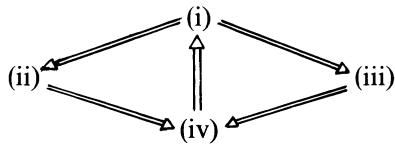
\includegraphics[keepaspectratio]{images/part002_fd83f186.jpg}}

If \(u\) is surjective, it is a strict morphism (IV, p.~28, th. 1) then for every semi-norm \(p \in \mathrm{S}(\mathrm{E})\) , there exists a semi-norm \(q \in \mathrm{S}(\mathrm{F})\) such that, for all \(y \in \mathrm{F}\) satisfying \(q(y) \leqslant 1\) , there exists \(x \in \mathrm{E}\) satisfying \(p(x) \leqslant 1\) and \(u(x) = y\) . We deduce immediately that (i) implies (ii) and (iii). It is clear that (ii) implies (iv).

To prove that (iii) implies (iv), let \(p\) and \(q\) be as in (iii). Let \(y \in \mathbf{F}\) , by (iii), there exists \(x\) in \(\mathbf{E}\) such that \(q(u(x) - y) = 0\) . If \(f \in \mathbf{F}'\) satisfies \(|f \circ u| \leqslant p\) , then we have \(f(u(x) - y) = 0\) , hence

\[
\left| f (y) \right| = \left| f (u (x)) \right| \leqslant p (x)
\]

and the relation (1) is satisfied.

Finally we prove that (iv) implies (i). Let \(p \in \mathrm{S}(\mathrm{E})\) and let \(q\) be the superior envelope of the functions \(|f|\) for \(f \in \mathrm{F}'\) satisfying \(|f \circ u| \leqslant p\) . By (iv), \(q\) is finite on \(\mathrm{F}\) , and is evidently a lower semi-continuous semi-norm on \(\mathrm{F}\) ; since \(\mathrm{F}\) is barrelled (III, p.~25, corollary), we have \(q \in \mathrm{S}(\mathrm{F})\) . Let \(\mathbf{B}_p\) (resp. \(\mathbf{B}_q\) ) denote the set of all \(x \in \mathrm{E}\) (resp. \(y \in \mathrm{F}\) ) such that \(p(x) \leqslant 1\) (resp. \(q(y) \leqslant 1\) ). We have \(q \circ u \leqslant p\) , and so \(u(\mathbf{B}_p) \subset \mathbf{B}_q\) . The polar of \(u(\mathbf{B}_p)\) in \(\mathrm{F}'\) consists of linear forms \(f \in \mathrm{F}'\) such that \(|f \circ u| \leqslant p\) , hence \(|f| \leqslant q\) ; in other words, we get \(u(\mathbf{B}_p)^{\circ} \subset \mathbf{B}_q^{\circ}\) , and finally that \(\overline{u(\mathbf{B}_p)} = \mathbf{B}_q\) follows from the theorem of bipolars (II, p.~45, cor. 3). If \(\mathrm{U}\) is a neighbourhood of 0 in \(\mathrm{E}\) , there exists \(p \in \mathrm{S}(\mathrm{E})\) such that \(\mathbf{B}_p \subset \mathbf{U}\) , hence \(\overline{u(\mathbf{U})}\) contains the neighbourhood \(\mathbf{B}_q\) of 0 in \(\mathrm{F}\) . This implies that \(u\) is surjective (I, p.~17, th. 1).

COROLLARY. --- Suppose E and F are Banach spaces. The following conditions are equivalent :

\begin{enumerate}
\def\labelenumi{(\roman{enumi})}
\item
  \(u\) is surjective.
\item
  There exists a real number \(r > 0\) , such that \(\| f \| \leqslant r\) . \(\| {}^t u(f) \|\) for all \(f \in \mathbf{F}'\) .
\item
  For all \(y \in F\) , we have \(\sup_{\substack{f\in \mathbf{F}^{\prime}\\ |f\circ u|\leqslant 1}} |f(y)| < +\infty\) .
\end{enumerate}

The conditions (ii) and (iii) are in fact reformulations of conditions (ii) and (iv) of prop. 4 for Banach spaces.

\section{COMPACTNESS CRITERIA}

\subsection{General remarks}

Let A be a subset of a topological space E. For a sequence \((x_{n})_{n\in\mathbf{N}}\) of points of A to have a point x of E as a limit point, it is necessary and sufficient that the following condition is satisfied (GT, I, § 7, No.~3):

\begin{enumerate}
\def\labelenumi{(\Alph{enumi})}
\tightlist
\item
  For every integer \(m \geqslant 0\) and every neighbourhood \(\mathbf{U}\) of \(x\) , there exists an integer \(n \geqslant m\) such that \(x_{n} \in \mathbf{U}\) .
\end{enumerate}

A sequence of the form \((y_{k})_{k\in\mathbb{N}}\) with \(y_{k}=x_{n_{k}}\) for a strictly increasing sequence \((n_{k})_{k\in\mathbb{N}}\) of positive integers is called an extracted sequence of the sequence \((x_{n})_{n\in\mathbb{N}}\) . If there exists an extracted sequence of the sequence \((x_{n})_{n\in\mathbb{N}}\) which converges to x, then x is a limit point of \((x_{n})\) ; conversely, if x has a countable fundamental system of neighbourhoods, and x is the limit point of the sequence \((x_{n})\) , then there exists an extracted sequence of \((x_{n})\) converging to x.

On account of GT, IX, § 2, No.~9, corollary, we conclude that when E is metrizable, the following conditions are equivalent :

\begin{enumerate}
\def\labelenumi{\alph{enumi})}
\item
  the set A is relatively compact in E;
\item
  every infinite sequence of points of A has a limit point in E;
\item
  from every infinite sequence of points of A, we can extract a sequence which converges to a point of E.
\end{enumerate}

In this section, we shall extend this criterion to certain non metrizable topological vector spaces. The following proposition enables us to reduce the study of compact sets to that of weakly compact sets in a number of cases.

PROPOSITION 1. --- Let E be a Hausdorff locally convex space, and A a subset of E. Let \(E_{\sigma}\) denote the space E with the weakened topology.

\begin{enumerate}
\def\labelenumi{\alph{enumi})}
\item
  If every infinite sequence of points of \(\mathbf{A}\) has a limit point in \(\mathbf{E}\) , then \(\mathbf{A}\) is precompact in \(\mathbf{E}\) .
\item
  In order that A be relatively compact in E, it is necessary and sufficient that it is precompact in E and relatively compact in \(E_{\sigma}\) .
\end{enumerate}

We shall prove \(a)\) by reductio ad absurdum. If \(A\) is not precompact, then by th. 3 of GT, II, § 3, No.~7, it follows that there exists a symmetric convex neighbourhood \(V\) of 0 in \(E\) such that \(A\) cannot be covered by a finite number of translates of \(V\) .

In other words, if \(x_{0}, x_{1}, \ldots, x_{n-1}\) are points of A, then \(A \not\subset \bigcup_{0 \leqslant i < n} (x_{i} + V)\) and so there exists a point \(x_{n}\) of A such that \(x_{n} - x_{i} \notin V\) for \(0 \leqslant i < n\) . Then, by induction on the integer n, we can construct an infinite sequence \((x_{n})_{n \in \mathbb{N}}\) of points of A such that \(x_{n} - x_{m} \notin V\) whenever n \textgreater{} m; since V is symmetric, we also have \(x_{m} - x_{n} \notin V\) for \(m \neq n\) and the sets \(x_{n} + \frac{1}{2}V\) are disjoint. For every point x in E, there exists at most one integer \(n \geqslant 0\) such that \(x_{n} \in x + \frac{1}{2}V\) , hence the sequence \((x_{n})_{n \in \mathbb{N}}\) does not have any limit point. This proves a).

Now suppose that A is precompact in E and is contained in a compact subset B of \(E_{\sigma}\) . Then B is complete in \(E_{\sigma}\) , hence also in E (IV, p.~5, Remark 2). We have \(\overline{A} \subset B\) , hence A is relatively compact in E. The converse is evident and b) follows.

\subsection{Simple compactness of sets of continuous functions}

In this section, X denotes a compact space and \(\mathcal{C}_{s}(X)\) the space of continuous functions on X, with values in the field K (equal to R or C). The space \(\mathcal{C}_{s}(X)\) is assigned the topology of simple convergence on X.

PROPOSITION 2. --- Let D be a dense subset of X and A a subset of the space \(\mathcal{C}_{s}(X)\) . The following conditions are equivalent :

\begin{enumerate}
\def\labelenumi{(\roman{enumi})}
\item
  A is relatively compact in \(\mathcal{C}_s(\mathbf{X})\) .
\item
  From every infinite sequence of elements of \(\mathbf{A}\) , we can extract a sequence converging in \(\mathcal{C}_s(\mathbf{X})\) .
\item
  Every infinite sequence of elements of \(\mathbf{A}\) has a limit point in \(\mathcal{C}_s(\mathbf{X})\) .
\item
  Let \((f_n)_{n\in \mathbb{N}}\) be a sequence of functions belonging to A and \((x_m)_{m\in \mathbb{N}}\) a sequence of points of D. If the iterated limits
\end{enumerate}

\[
\gamma = \lim _ {m \rightarrow \infty} \lim _ {n \rightarrow \infty} f _ {n} (x _ {m}), \quad \delta = \lim _ {n \rightarrow \infty} \lim _ {m \rightarrow \infty} f _ {n} (x _ {m})
\]

exist, then they are equal. In addition, we have \(\sup_{f\in \mathbf{A}}|f(x)| < +\infty\) for all \(x\in \mathbf{X}\) .

\begin{enumerate}
\def\labelenumi{(\roman{enumi})}
\tightlist
\item
  \(\Rightarrow\) (ii): let \(\overline{\mathbf{A}}\) be the closure of \(\mathbf{A}\) in \(\mathcal{C}_s(\mathbf{X})\) . Assume that \(\mathbf{A}\) is compact, and consider a sequence of functions \(f_n \in \mathbf{A}\) (for \(n \in \mathbf{N}\) ). Let \(\phi\) be the continuous mapping \(x \mapsto (f_n(x))_{n \in \mathbf{N}}\) from \(\mathbf{X}\) into the metrizable space \(\mathbf{K}^{\mathbf{N}}\) . The image \(\mathbf{X}'\) of \(\mathbf{X}\) under \(\phi\) is a compact metrizable space, since \(\mathbf{X}\) is compact. Let \(\mathbf{E}\) be the closed subspace of \(\mathcal{C}_s(\mathbf{X})\) consisting of continuous functions \(f\) on \(\mathbf{X}\) such that the relation \(\phi(x) = \phi(y)\) implies \(f(x) = f(y)\) for every pair of points \(x, y\) in \(\mathbf{X}\) . By cor. 2 of GT, I, § 9, No.~4 and prop. 3 of GT, I, § 5, No.~2, the mapping \(f' \mapsto f' \circ \phi\) is a homeomorphism \(\phi^*\) from \(\mathcal{C}_s(\mathbf{X}')\) onto E. Hence the set \(\mathbf{A}' = (\phi^*)^{-1}(\overline{\mathbf{A}})\) is compact in \(\mathcal{C}_s(\mathbf{X}')\) , and it is clear that there exist elements \(f_n'\) in \(\mathbf{A}'\) such that \(\phi^*(f_n') = f_n' \circ \phi\) is equal to \(f_n\) .
\end{enumerate}

Since \(X'\) is a compact metrizable space, there exists a countable dense subset \(D'\) in \(X'\) (GT, IX, §2, No.~8, prop. 12 and §2, No.~9, prop. 16). Let \(T_{1}\) (resp. \(T_{2}\) ) be the topology on \(A'\) induced by the topology of simple convergence on \(D'\) (resp. \(X'\) ). Then \(T_{1}\) is metrizable, \(T_{2}\) is compact and finer than \(T_{1}\) , hence \(T_{1}\) and \(T_{2}\) coincide; in other words, \(A'\) is a compact metrizable subspace of \(\mathcal{C}_{s}(X')\) . Therefore, there exists a sequence \((f_{n_k}^{\prime})\) extracted from \((f_n^{\prime})\) and converging to an element \(f^{\prime}\) of \(\mathcal{C}_s(\mathbf{X}')\) . Therefore, the sequence \((f_{n_k})\) converges to \(f = f' \circ \phi\) in \(\mathcal{C}_s(\mathbf{X})\) .

\begin{enumerate}
\def\labelenumi{(\roman{enumi})}
\setcounter{enumi}{1}
\item
  \(\Rightarrow\) (iii): this is clear.
\item
  \(\Rightarrow\) (iv): suppose that every infinite sequence of elements of A has a limit point in \(\mathcal{C}_s(\mathbf{X})\) . Let \(x \in \mathbf{X}\) . The mapping \(\phi_x: f \mapsto f(x)\) from A into K is continuous. Consequently, every infinite sequence in \(\phi_x(\mathbf{A})\) has a limit point; since the field K (equal to R or C) is metrizable, the set \(\phi_x(\mathbf{A})\) is relatively compact in K, hence bounded. In other words, we have \(\sup_{f \in \mathbf{A}} |f(x)| < \infty\) .
\end{enumerate}

Let \(f_n, x_m, \gamma\) and \(\delta\) be as in (iv). Let \(f\) be a limit point of the sequence \((f_n)\) in \(\mathcal{C}_s(\mathbf{X})\) , and let \(x\) be a limit point of the sequence \((x_m)\) in the compact space \(\mathbf{X}\) . For every \(m\) , the mapping \(h \mapsto h(x_m)\) from \(\mathcal{C}_s(\mathbf{X})\) into \(\mathbf{K}\) is continuous. In view of the hypotheses, we have \(f(x_m) = \lim_{n \to \infty} f_n(x_m)\) , and hence \(\gamma = \lim_{m \to \infty} f(x_m)\) ; since \(f: \mathbf{X} \to \mathbf{K}\) is continuous and \(x\) is a limit point of the sequence \((x_m)\) , we get \(\gamma = f(x)\) . In an analogous way, we prove the equality \(\delta = f(x)\) , whence \(\gamma = \delta\) .

\begin{enumerate}
\def\labelenumi{(\roman{enumi})}
\setcounter{enumi}{3}
\tightlist
\item
  \(\Rightarrow\) (i): suppose that the set of numbers \(f(x)\) , as \(f\) ranges over \(\mathbf{A}\) , is bounded in \(\mathbf{K}\) for all \(x\in \mathbf{X}\) . This is equivalent to assuming that the closure \(\overline{\mathbf{A}}\) of \(\mathbf{A}\) in the product space \(\mathbf{K}^{\mathbf{X}}\) is compact (GT, I, § 9, No.~5). Suppose that \(\mathbf{A}\) is not relatively compact in \(\mathcal{C}_s(\mathbf{X})\) . This means that there exists a function \(u\in \overline{\mathbf{A}}\) and a point \(a\in \mathbf{X}\) such that \(u\) is not continuous at \(a\) . Hence there exists a real number \(\varepsilon >0\) such that in every neighbourhood \(\mathrm{U}\) of \(a\) , there exists a point \(x\) with \(|u(x) - u(a)|\geqslant \varepsilon\) .
\end{enumerate}

We shall construct by induction a sequence \((x_{n})_{n\in \mathbf{N}}\) of points in \(\mathbf{D}\) and a sequence \((f_n)_{n\in \mathbf{N}}\) of elements of \(\mathbf{A}\) , satisfying the following relations:

\[
\left| u (x _ {m}) - u (a) \right| \geqslant \varepsilon \quad \text { for } \quad m \geqslant 1;\tag{$(1)_{m}$}
\]

\[
\left| u (x _ {i}) - f _ {m} (x _ {i}) \right| \leqslant \frac {1}{m + 1} \text { for } 0 \leqslant i \leqslant m - 1;\tag{$(2)_{m}$}
\]

\[
\left| f _ {m} (x _ {i}) - f _ {m} (a) \right| \leqslant \frac {1}{i + 1} \quad \text { for } \quad 0 \leqslant m \leqslant i.\tag{$(3)_{m,i}$}
\]

We take \(x_0 = a\) with \(f_0\) arbitrary in A (the set A is not empty, otherwise it will be relatively compact in \(\mathcal{C}_s(\mathbf{X})\) ). Let \(n \geqslant 1\) and \(x_0, x_1, \ldots, x_{n-1}, f_0, f_1, \ldots, f_{n-1}\) satisfy relations \((1)_m, (2)_m\) for \(1 \leqslant m < n\) and \((3)_{m,i}\) for \(0 \leqslant m \leqslant i < n\) . Since \(u\) belongs to \(\overline{\mathbf{A}}\) , there exists \(f_n \in \mathbf{A}\) satisfying \((2)_n\) . Let \(V_n\) be the set of all \(x \in X\) such that \(|f_m(x) - f_m(a)| \leqslant \frac{1}{n+1}\) for \(0 \leqslant m \leqslant n\) . Since \(f_n\) is continuous, \(V_n\) is a neighbourhood of \(a\) ; choose a point \(x_n\) in \(D \cap V_n\) such that \(|u(x_n) - u(a)| \geqslant \varepsilon\) , hence \((1)_n\) and \((3)_{m,n}\) are satisfied. Therefore, the construction can be continued.

Since \(u(\mathbf{X})\) is a compact subset of \(\mathbf{K}\) , there exists a sequence \((y_k)\) extracted from \((x_m)\) and such that the limit \(\gamma = \lim_{k\to \infty}u(y_k)\) exists. By (2) \(_m\) , we have \(u(x_i) = \lim_{n\to \infty}f_n(x_i)\) for all \(i\in \mathbf{N}\) , hence

\[
\gamma = \lim _ {k \rightarrow \infty} \lim _ {n \rightarrow \infty} f _ {n} (y _ {k}).\tag{4}
\]

On the other hand we have \(f_{n}(a) = \lim_{i\to \infty}f_{n}(x_{i})\) by (3) \(_{m,i}\) hence \(f_{n}(a) = \lim_{k\to \infty}f_{n}(y_{k})\) . Since \(x_0 = a\) , we deduce from (2) \(_{m}\) that \(\lim_{n\to \infty}f_n(a) = u(a)\) . Consequently,

\[
u (a) = \lim _ {n \rightarrow \infty} \lim _ {k \rightarrow \infty} f _ {n} (y _ {k}).\tag{5}
\]

Finally, from \((1)_{m}\) , we get \(|\gamma - u(a)| \geqslant \varepsilon\) , and so \(\gamma \neq u(a)\) . This contradicts assertion (iv); we have thus proved that (iv) implies (i).

\subsection{The Eberlein and Šmulian theorems}

THEOREM 1 (Eberlein). --- Let E be a Hausdorff and quasi-complete locally convex space, T a topology on E which is compatible with the duality between E and E' and A a subset of E. For A to be relatively compact for T, it is necessary and sufficient that every infinite sequence of points of A has a limit point in E for T.

The condition stated is obviously necessary.

Suppose now that every infinite sequence of points of A has a limit point for T, hence also for the coarser topology \(\sigma(\mathrm{E}, \mathrm{E}')\) . Then A is precompact for T (IV, p.~32, prop. 1); in order that A be relatively compact for T, it is necessary and sufficient that it be so for \(\sigma(\mathrm{E}, \mathrm{E}')\) (loc. cit.). Therefore it is enough to prove the theorem when T is the weakened topology \(\sigma(\mathrm{E}, \mathrm{E}')\) .

Let \(\hat{\mathrm{E}}\) denote the completion of E, which we shall identify as usual with a subspace of the algebraic dual \(\mathrm{E}^{\prime *}\) of \(\mathrm{E}'\) (III, p.~21, th. 2). Let \(\mathrm{E}_{\sigma}\) , \(\hat{\mathrm{E}}_{\sigma}\) and \(\mathrm{E}_{\sigma}^{\prime *}\) denote the spaces E, \(\hat{\mathrm{E}}\) and \(\mathrm{E}^{\prime *}\) endowed with the topologies \(\sigma (\mathrm{E},\mathrm{E}')\) , \(\sigma (\hat{\mathrm{E}},\mathrm{E}')\) and \(\sigma (\mathrm{E}^{\prime *},\mathrm{E}^{\prime})\) respectively.

Let \((x_{i}^{\prime})_{i\in\mathbb{I}}\) be a basis of the vector space \(E^{\prime}\) over the field K. The mapping \(f\mapsto(f(x_{i}^{\prime}))_{i\in\mathbb{I}}\) is a homeomorphism \(\phi\) from \(E_{\sigma}^{\prime*}\) onto \(K^{I}\) ; for every \(i\in I\) , the image of A under the mapping \(x_{i}^{\prime}\) from E into K is relatively compact: for, K is metrizable and every infinite sequence of elements of \(x_{i}^{\prime}(A)\) has a limit point. It follows that \(\phi(A)\) is relatively compact in \(K^{I}\) , hence that the closure \(\overline{A}\) of A in \(E_{\sigma}^{\prime*}\) is compact.

Next we shall prove that \(\overline{A}\) is contained in \(\hat{E}\) . Let H be an equicontinuous subset of \(E'\) ; let X be its closure for \(\sigma(E', E)\) ; X is compact (III, p.~17, cor. 2). For every \(x \in E'^{*}\) , let \(\phi_{x}\) be the restriction of \(x' \mapsto \langle x, x' \rangle\) to X; let \(\tilde{A} \subset \mathcal{C}_{s}(X)\) be the set of functions \(\phi_{x}\) as x ranges over A. In view of the hypothesis on A, every infinite sequence of elements of \(\tilde{A}\) has a limit point in \(\mathcal{C}_{s}(X)\) ; by prop. 2 (IV, p.~33), the set \(\tilde{A}\) is therefore relatively compact in \(\mathcal{C}_{s}(X)\) . It follows that for every \(a \in \overline{A}\) , the function \(\phi_{a}\) on X is continuous. The inclusion \(\overline{A} \subset \hat{E}\) then follows from th. 2 of III, p.~21.

Now we shall show that \(\overline{\mathbf{A}}\) is contained in E. Since A is precompact in \(\mathrm{E}_{\sigma}\) (IV, p.~32, prop. 1), it is bounded in \(\mathrm{E}_{\sigma}\) (III, p.~3, prop. 2), hence also in E (IV, p.~1, prop. 1). Let C be the closed convex balanced envelope of A in E. Then C is bounded since A is bounded, hence complete since E is quasi-complete. In other words, C is a convex and closed subset of \(\hat{\mathrm{E}}\) , so also of \(\hat{\mathrm{E}}_{\sigma}\) (IV, p.~1, prop. 1). Since \(\mathbf{A} \subset \mathbf{C}\) and the topology of \(\hat{\mathrm{E}}_{\sigma}\) is induced by that of \(\mathrm{E}_{\sigma}^{\prime *}\) , we have \(\overline{\mathbf{A}} \subset \mathbf{C}\) , and hence \(\overline{\mathbf{A}} \subset \mathbf{E}\) .

Since the topology of \(E_{\sigma}\) is induced by that of \(E_{\sigma}^{\prime*}\) , the subset \(\overline{A}\) of \(E_{\sigma}\) is compact, and th. 1 follows.

THEOREM 2 (Šmulian). --- Let E be a Fréchet space and A a subset of E. Let \(E_{\sigma}\) denote the space E endowed with the weakened topology. The following conditions are equivalent :

\begin{enumerate}
\def\labelenumi{(\roman{enumi})}
\item
  A is relatively compact in \(\mathrm{E}_{\sigma}\) ;
\item
  every infinite sequence of points of A has a limit point in \(\mathrm{E}_{\sigma}\) ;
\item
  from every infinite sequence of points of \(\mathbf{A}\) , we can extract a sequence which converges in \(\mathrm{E}_{\sigma}\) .
\end{enumerate}

The equivalence of (i) and (ii) follows from Eberlein's theorem and (iii) obviously implies (ii).

We shall prove that (i) implies (iii). Suppose that the closure B of A in \(E_{\sigma}\) is compact and that \((x_{n})_{n\in\mathbf{N}}\) is a sequence of points of A. Let F denote the smallest closed vector subspace of E containing the \(x_{n}\) , this is a Fréchet space satisfying the first axiom of countability. Since F is closed in \(E_{\sigma}\) and the topology \(\sigma(\mathrm{F},\mathrm{F}')\) on F is induced by \(\sigma(\mathrm{E},\mathrm{E}')\) , the set \(B\cap F\) is compact for \(\sigma(\mathrm{F},\mathrm{F}')\) . On account of the remarks in IV, p.~32, the existence of a sequence extracted from \((x_{n})_{n\in\mathbf{N}}\) converging for \(\sigma(\mathrm{E},\mathrm{E}')\) (or, which is the same, for \(\sigma(\mathrm{F},\mathrm{F}')\) ) is a consequence of the following lemma:

Lemma 1. --- Let F be a Fréchet space satisfying the first axiom of countability. Every subset C of F which is compact for the topology T induced by \(\sigma(\mathrm{F},\mathrm{F}')\) is metrizable for this topology.

Since the topology of precompact convergence on \(F'\) is finer than the topology \(\sigma(F', F)\) , there exists an everywhere dense countable subset in \(F_{s}'\) (III, p.~18, cor. 1). Hence the set C can be identified with a subset of \(K^{D}\) , and the topology induced on C by that of \(K^{D}\) , which is metrizable (GT, IX, § 2, No.~8) is coarser than the topology induced by \(\sigma(F, F')\) , for which C is compact. Hence these two topologies are identical (GT, I, § 9, No.~4, cor. 3).

Šmulian's theorem can be extended to the case where E is the strict inductive limit of a sequence of Fréchet spaces (IV, p.~67, exerc. 2).

\subsection{* The case of spaces of bounded continuous functions}

For every topological space X, let \(\mathcal{C}^{b}(X)\) denote the Banach space of all continuous and bounded mappings from X into K, with the norm defined by

\[
\| f \| = \sup _ {x \in X} | f (x) |\tag{6}
\]

(GT, X, § 3, No.~2). When X is compact, every continuous function on X is bounded (GT, IV, § 6, No.~1), and we write \(\mathcal{C}(X)\) for \(\mathcal{C}^b(X)\) .

In this and the following section, we shall use the following lemma, which is a particular case of Lebesgue's theorem (INT, IV, 2nd ed.~§ 4, No.~3, th. 2) on account of the interpretation of the elements of \(\mathcal{C}(\mathrm{X})'\) as measures on X.

Lemma 2. --- Let X be a compact space. If a sequence \((f_n)_{n\in \mathbf{N}}\) is bounded in \(\mathcal{C}(\mathbf{X})\) and converges simply on X to a continuous function \(f\) , then \(\mu(f) = \lim_{n\to \infty}\mu(f_n)\) for every \(\mu\) in \(\mathcal{C}(\mathbf{X})'\) .

PROPOSITION 3. --- Let X be a compact space, and let A be a bounded subset of \(\mathcal{C}(\mathrm{X})\) . For A to be relatively compact for the topology of simple convergence, it is necessary and sufficient that it is relatively compact for \(\sigma(\mathcal{C}(\mathrm{X}), \mathcal{C}(\mathrm{X})')\) .

The topology of simple convergence is Hausdorff and coarser than \(\sigma(\mathcal{C}(X), \mathcal{C}(X)')\) , hence the condition stated is sufficient (GT, I, § 9, No.~4, cor. 3).

Now suppose that A is relatively compact for the topology of simple convergence. Let \((f_{n})_{n\in\mathbf{N}}\) be a sequence of elements of A. By prop. 2 (IV, p.~33), there exists a sequence \((f_{n_{k}})\) extracted from \((f_{n})\) and converging simply to a continuous function f.~By lemma 2, the bounded sequence \((f_{n_{k}})\) tends to f for \(\sigma(\mathcal{C}(\mathrm{X}),\mathcal{C}(\mathrm{X})')\) . Then Šmulian's theorem (IV, p.~36, th. 2) shows that A is relatively compact for \(\sigma(\mathcal{C}(\mathrm{X}),\mathcal{C}(\mathrm{X})')\) .

COROLLARY. --- Let S be a topological space and A a bounded subset of \(\mathcal{C}^{b}(S)\) . The following conditions are equivalent :

\begin{enumerate}
\def\labelenumi{(\roman{enumi})}
\item
  A is relatively compact for \(\sigma(\mathcal{C}^b(\mathbf{S}),\mathcal{C}^b(\mathbf{S})')\) ;
\item
  if \((f_n)_{n\in \mathbb{N}}\) is a sequence of elements of \(\mathbf{A}\) and \((x_m)_{m\in \mathbb{N}}\) is a sequence of points of \(\mathbf{S}\) such that the iterated limits
\end{enumerate}

\[
\gamma = \lim _ {m \rightarrow \infty} \lim _ {n \rightarrow \infty} f _ {n} (x _ {m}), \quad \delta = \lim _ {n \rightarrow \infty} \lim _ {m \rightarrow \infty} f _ {n} (x _ {m})
\]

exist, then \(\gamma = \delta\) .

Let X be the Stone-Čech compactification of S (GT, IX, § 1, No.~6) and \(\alpha\) the canonical mapping from S into X. Put \(D = \alpha(S)\) . The mapping \(\phi: f \mapsto f \circ \alpha\) is an isomorphism from the normed space \(\mathcal{C}(X)\) onto the normed space \(\mathcal{C}^b(S)\) ; put \(\tilde{A} = \phi^{-1}(A)\) . Since X is compact and D is dense in X, the prop. 2 (IV, p.~33) shows that condition (ii) is equivalent to the compactness of \(\tilde{A}\) for the topology of simple convergence. The equivalence of (i) and (ii) then follows from prop. 3. *

\subsection{* Convex envelope of a weakly compact set}

THEOREM 3 (Krein). --- Let E be a Hausdorff and quasi-complete locally convex space, and let T be a topology on E compatible with the duality between E and E'. Let A be a subset of E which is compact for T. Then the closed convex balanced envelope C of A is compact for T.

We shall first make several reductions.

\begin{enumerate}
\def\labelenumi{\Alph{enumi})}
\item
  The set C is precompact for \(\mathcal{T}\) (II, p.~25, prop. 3), and A is compact for \(\sigma(\mathrm{E}, \mathrm{E}')\) . On account of prop. 1 (IV, p.~32), it is enough to prove that C is compact for \(\sigma(\mathrm{E}, \mathrm{E}')\) , and so we have reduced to the case where \(\mathcal{T} = \sigma(\mathrm{E}, \mathrm{E}')\) .
\item
  Since C is precompact and closed for \(\sigma(\mathrm{E}, \mathrm{E}')\) , it is bounded and closed for the initial topology of E (III, p.~3, prop. 2 and IV, p.~1, prop. 1); hence it is complete since E is quasi-complete. In other words, C is the closed convex balanced envelope of A in the completion \(\hat{\mathbf{E}}\) of E. Since the topology \(\sigma (\hat{\mathbf{E}},\mathrm{E}^{\prime})\) induces \(\sigma (\mathrm{E},\mathrm{E}^{\prime})\) on E, we have reduced to the case when E is complete.
\item
  Let \(\Gamma\) be the convex balanced envelope of A. Then C is the closure of \(\Gamma\) for \(\sigma(E, E')\) . By Eberlein's theorem (IV, p.~35, th. 1), it is enough to prove that every sequence \((x_n)_{n \in \mathbf{N}}\) of points of \(\Gamma\) has a limit point for \(\sigma(E, E')\) in E. But \(x_n\) belongs to the convex balanced envelope of a finite subset \(\mathbf{B}_n\) of A. Let F be the closed vector subspace of E generated by the countable set \(\mathbf{B} = \bigcup_{n} \mathbf{B}_n\) . Then F is complete, the topology \(\sigma(F, F')\) on F is induced by \(\sigma(E, E')\) and we have \(x_n \in F\) for all \(n \in \mathbf{N}\) . Hence it is enough to prove that \((x_n)_{n \in \mathbf{N}}\) has a limit point for \(\sigma(F, F')\) , which gives the reduction to the case when there exists a countable dense set in E.
\end{enumerate}

Let A be assigned the topology induced by \(\sigma(E, E')\) , which makes it a compact space. We define a linear mapping \(u: E' \to \mathcal{C}(A)\) by

\[
u (x ^ {\prime}) (a) = \langle a, x ^ {\prime} \rangle \quad (a \in \mathrm{A}, x ^ {\prime} \in \mathrm{E} ^ {\prime}).\tag{7}
\]

Let \((x_{n}^{\prime})_{n\in\mathbb{N}}\) be an equicontinuous sequence in E', converging to 0 for \(\sigma(\mathrm{E}^{\prime},\mathrm{E})\) . Then the sequence of functions \(u(x_{n}^{\prime})\) is bounded in \(\mathcal{C}(\mathrm{A})\) and converges simply to 0. For every \(\mu\in\mathcal{C}(\mathrm{A})^{\prime}\) , we have \(\lim_{n\to\infty}\mu(u(x_{n}^{\prime}))=0\) by lemma 2 (IV, p.~37). By the criterion given in the remark in III, p.~21, the linear form \(\mu\circ u\) on E' is then continuous for \(\sigma(\mathrm{E}^{\prime},\mathrm{E})\) for every \(\mu\in\mathcal{C}(\mathrm{A})^{\prime}\) . Hence there exists a linear mapping \(v:\mathcal{C}(\mathrm{A})^{\prime}\to\mathrm{E}\) satisfying the relation

\[
\langle u (x ^ {\prime}), \mu \rangle = \langle v (\mu), x ^ {\prime} \rangle \quad \left(x ^ {\prime} \in \mathrm{E} ^ {\prime}, \mu \in \mathcal {C} (\mathrm{A}) ^ {\prime}\right).\tag{8}
\]

It is clear that \(v\) is continuous if \(\mathcal{C}(\mathbf{A})'\) is assigned the topology \(\sigma(\mathcal{C}(\mathbf{A})', \mathcal{C}(\mathbf{A}))\) and \(E\) the topology \(\sigma(E, E')\) .

The unit ball (closed) B of the Banach space \(\mathcal{C}(\mathrm{A})\) is compact for the topology \(\sigma(\mathcal{C}(\mathrm{A})', \mathcal{C}(\mathrm{A}))\) (III, p.~17, cor. 3). Consequently, \(v(\mathrm{B})\) is a convex balanced and compact subset of E for \(\sigma(\mathrm{E}, \mathrm{E}')\) . For every \(a \in A\) , the continuous linear form \(\varepsilon_a : f \mapsto f(a)\) on \(\mathcal{C}(\mathrm{A})\) belongs to B, and we have \(v(\varepsilon_a) = a\) by formulas (7) and (8). Hence, \(A \subset v(\mathrm{B})\) , and so \(C \subset v(\mathrm{B})\) . This proves that C is compact for \(\sigma(\mathrm{E}, \mathrm{E}')\) .

Q.E.D.

\chapterappendix{Fixed points of groups of affine transformations}

\subsection{The case of solvable groups}

Let \(\mathbf{E}\) be a real vector space, and \(\mathbf{K}\) a convex subset of \(\mathbf{E}\) . A mapping \(u: \mathbf{K} \to \mathbf{K}\) such that for \(x, y\) in \(\mathbf{K}\) and for every real number \(t\) in \([0, 1]\) , we have

\[
u (t x + (1 - t) y) = t u (x) + (1 - t) u (y)\tag{1}
\]

is said to be an affine transformation. From relation (1) we deduce that

\[
u \left(\sum_ {i \in \mathrm{I}} t _ {i} x _ {i}\right) = \sum_ {i \in \mathrm{I}} t _ {i} u \left(x _ {i}\right)\tag{2}
\]

for every finite set I, points \(x_{i}\) in K and positive real numbers \(t_i\) such that \(\sum_{i\in I}t_i = 1\) .

Let u and v be two affine transformations on K, then the mapping \(u \circ v\) is an affine transformation on K. If \(v: E \to E\) is a linear mapping such that \(v(\mathbf{K}) \subset \mathbf{K}\) , the mapping \(u: K \to K\) which coincides with v on K is an affine transformation.

THEOREM 1 (Markoff-Kakutani). --- Let E be a Hausdorff locally convex vector space over the field R, and K a non-empty compact convex subset of E. Let \(\Gamma\) be a set of continuous affine transformations on K, pairwise permutable. Then there exists a point a in K such that \(u(a) = a\) for all \(u \in \Gamma\) .

For every \(u \in \Gamma\) , let \(\mathbf{K}_u\) be the set of all \(x \in \mathbf{K}\) such that \(u(x) = x\) . We shall show that \(\mathbf{K}_u\) is non-empty. Let \(x\) be a point of \(\mathbf{K}\) ; for every integer \(n \geqslant 1\) , let \(x_n\) be the element \(\frac{1}{n} \sum_{i=0}^{n-1} u^i(x)\) of \(\mathbf{E}\) . Since \(\mathbf{K}\) is convex and stable under \(u\) , the points \(x_n\) belong to \(\mathbf{K}\) and since \(\mathbf{K}\) is compact, there exists a limit point \(a\) of the sequence \((x_n)_{n \geqslant 1}\) . The mapping \(y \mapsto u(y) - y\) from \(\mathbf{K}\) into \(\mathbf{E}\) is continuous, hence \(u(a) - a\) is a limit point of the sequence \((u(x_n) - x_n)_{n \geqslant 1}\) . But we have \(u(x_n) - x_n = \frac{1}{n} (u^n(x) - x)\) .

Since K is compact, hence also bounded (III, p.~3, prop. 2), the sequence \((u^n(x) - x)_{n\geqslant 1}\) is bounded; consequently, the sequence \(\left(\frac{1}{n} (u^n (x) - x)\right)_{n\geqslant 1}\) tends to 0 (III, p.~4, prop. 3), and since E is Hausdorff, we have \(u(a) - a = 0\) . Therefore \(a\in \mathbf{K}_u\) .

Each of the sets \(\mathbf{K}_u\) is a closed and convex subset of the compact space \(\mathbf{K}\) , and we shall prove that the intersection \(\bigcap_{u\in \Gamma}\mathbf{K}_u\) is non-empty. For this it is enough to

prove that, for \(n \geqslant 1\) , and \(u_{1}, \ldots, u_{n}\) in \(\Gamma\) , the set \(K_{u_{1}} \cap \ldots \cap K_{u_{n}}\) is non-empty. The case n = 1 having been considered, we argue by induction on n.~Suppose \(n \geqslant 2\) and put \(L = K_{u_{1}} \cap \ldots \cap K_{u_{n-1}}\) . By the hypothesis of induction, L is a non-empty compact convex subset of E. Since \(u_{n}\) commutes with \(u_{1}, \ldots, u_{n-1}\) , we have \(u_{n}(L) \subset L\) . Applying the first part of the proof to the affine transformation induced by \(u_{n}\) on L, we conclude that there exists a point a in L such that \(u_{n}(a) = a\) ; then a belongs to \(K_{u_{1}} \cap \ldots \cap K_{u_{n}}\) , which is then non-empty.

COROLLARY. --- Let G be a solvable group of continuous affine transformations on K. Then there exists a point in K which is invariant under G.

By the definition of a solvable group (A, I, § 6, No.~4) there exists a finite decreasing sequence \((\mathbf{G}_i)_{0\leqslant i\leqslant n}\) of distinct subgroups of \(\mathbf{G}\) , such that \(\mathbf{G}_0 = \mathbf{G}\) , \(\mathbf{G}_n = \{e\}\) and such that the group \(\mathbf{G}_{i - 1} / \mathbf{G}_i\) is commutative for \(1\leqslant i\leqslant n\) . Let \(\mathbf{K}_i\) denote the set of fixed points of \(\mathbf{G}_i\) in \(\mathbf{K}\) . Then \(\mathbf{K}_n = \mathbf{K}\) . Moreover, for \(1\leqslant i\leqslant n\) , every element of \(\mathbf{G}_i\) induces the identity transformation on \(\mathbf{K}_i\) ; we thus deduce an action of the abelian group \(\mathbf{G}_{i - 1} / \mathbf{G}_i\) on \(\mathbf{K}\) if \(\mathbf{K}_i\) is non-empty; it follows from th. 1 that the set \(\mathbf{K}_{i - 1}\) of fixed points of \(\mathbf{G}_{i - 1} / \mathbf{G}_i\) in \(\mathbf{K}_i\) is non-empty. By descending induction on \(i\) , we conclude that \(\mathbf{K}_0\) is non-empty, hence the corollary.

\subsection{Invariant means}

Let X be a topological space. Let \(\mathcal{B}(\mathrm{X};\mathbf{R})\) denote the real vector space consisting of continuous bounded mappings from X into R. Endowed with the norm \(\| f\| = \sup_{x\in \mathbf{X}}|f(x)|\) , this is a Banach space (GT, X, § 3, No.~1); it is also an ordered vector space, where the relation \(f\geqslant g\) means \(\ll f(x)\geqslant g(x) \text{ for all } x\in \mathbf{X}\gg\) .

DEFINITION 1. --- A positive linear form \(\mu\) on the space \(\mathcal{B}(\mathbf{X};\mathbf{R})\) , where \(\mathbf{X}\) is a topological space, for which \(\|\mu\| = 1\) , is called a mean on \(\mathbf{X}\) .

* When X is compact, a mean on X is a positive measure on X such that \(\mu(X)=1\) . *

Lemma 1. --- The set K of means on X is the subset of the unit ball of the dual of the Banach space \(E = \mathcal{B}(X; \mathbf{R})\) whose elements are the linear forms \(\mu\) such that \(\mu(1)=1\) . It is a subset of \(E'\) which is convex and compact for \(\sigma(E', E)\) .

Let \(\mu\) be a linear form on \(E\) , such that \(\mu(1) = 1\) . For every function \(f \in E\) , we define the function \(f' \in E\) by \(f'(x) = \| f \| - f(x) (x \in X)\) . First assume that \(\mu\) is a mean; for every \(f \in E\) , we have \(f' \geqslant 0\) , hence \(\mu(f') \geqslant 0\) , i.e.~\(\mu(f) \leqslant \| f \|\) ; therefore \(\|\mu\| \leqslant 1\) .

Conversely, suppose \(\mu\) belongs to \(E'\) , and that \(\| \mu \| \leqslant 1\) ; for every positive function \(f \in E\) , we have \(\mu(f') \leqslant \| f'\|\) , hence

\[
\| f \| - \mu (f) = \mu \left(f ^ {\prime}\right) \leqslant \| f ^ {\prime} \| \leqslant \| f \|,
\]

and finally \(\mu(f) \geqslant 0\) ; consequently, \(\mu\) is a mean.

It is clear that K is convex; that it is compact for \(\sigma(\mathrm{E}^{\prime},\mathrm{E})\) follows from cor. 3 of III, p.~17.

Q.E.D.

Let \(\Gamma\) be a set of continuous mappings from X into X which commute pairwise. Let \(\gamma \in \Gamma\) . For every function \(f \in \mathbf{E}\) , we have \(f \circ \gamma \in \mathbf{E}\) ; hence we can define an affine transformation \(u_{\gamma}\) on the set K of means on X, by

\[
u _ {\gamma} \mu (f) = \mu (f \circ \gamma) (\mu \in \mathrm{K}, f \in \mathrm{E}).
\]

If K is assigned the topology induced by \(\sigma(\mathrm{E}^{\prime},\mathrm{E})\) , the mapping \(u_{\gamma}\) is continuous. If \(\gamma\) is a homeomorphism, \(u_{\gamma}\mu\) can be deduced from \(\mu\) by transport of structure. Finally, we have \(u_{\gamma}u_{\gamma^{\prime}} = u_{\gamma^{\prime}}u_{\gamma}\) for all \(\gamma\) , \(\gamma^{\prime}\) in \(\Gamma\) . By the Markoff-Kakutani th. (IV, p.~39, th. 1), there exists a mean \(\mu\) on X, such that \(u_{\gamma}\mu = \mu\) for all \(\gamma \in \Gamma\) ; in other words, \(\mu\) satisfies the relation \(\mu(f) = \mu(f \circ \gamma)\) for \(f \in E\) and \(\gamma \in \Gamma\) .

In an analogous way, the corollary of th. 1 (IV, p.~40) implies the following result :

PROPOSITION 1. --- Let X be a topological space and G a solvable group. We assume that G operates on X on the left, in such a way that for all \(g \in G\) , the mapping \(x \mapsto g \cdot x\) from X into X is continuous. Then there exists a mean on X which is invariant under G.

COROLLARY. --- Let G be a solvable topological group. Then there exists a mean on G which is invariant under the left and the right translations.

It is enough to apply prop. 1 to the solvable group \(\mathbf{G} \times \mathbf{G}\) acting on \(\mathbf{G}\) by \((g, g') \cdot x = gxg'^{-1}\) .

\subsection{Ryll-Nardzewski theorem}

In this section, E denotes a normed space over the field R and T a Hausdorff locally convex topology on E for which the norm of E is lower semi-continuous. These hypotheses are in particular satisfied in the following cases :

\begin{enumerate}
\def\labelenumi{\alph{enumi})}
\item
  \(\mathcal{T}\) is the topology induced by the norm of the normed space E.
\item
  \(\mathcal{T}\) is the weakened topology \(\sigma (\mathrm{E},\mathrm{E}^{\prime})\) of the normed space E.
\item
  E is the dual of a normed space F and \(\mathcal{T} = \sigma (\mathrm{F}',\mathrm{F})\)
\end{enumerate}

\(d\) ) There exist two normed spaces \(\mathrm{F}_1\) and \(\mathrm{F}_2\) such that \(\mathrm{E} = \mathcal{L}(\mathrm{F}_1;\mathrm{F}_2)\) and \(\mathcal{T}\) is the topology of simple convergence.

Unless otherwise expressly stated, the topological notions refer to the topology \(\mathcal{T}\) .

Let K be a convex subset of E. Suppose that K is compact (for the topology T), and that K satisfies the first axiom of countability for the distance defined by the norm of E.

Lemma 2. --- Suppose K contains at least two points. For every \(\varepsilon > 0\) , there exists a partition of K into two non-empty subsets \(\mathbf{K}_1\) and \(\mathbf{K}_2\) , having the following properties:

\begin{enumerate}
\def\labelenumi{\alph{enumi})}
\item
  \(\mathrm{K}_1\) is convex and compact;
\item
  we have \(\| x_1 - x_2\| < \varepsilon\) for every \(x_{1}\) and \(x_{2}\) in \(\mathbf{K}_2\) .
\end{enumerate}

Let L be the closure of the set of all extremal points of K. By the Krein-Milman th. (II, p.~55, th. 1), K is the closed convex envelope of L. Since K contains at least two points, so does L. For every \(x \in L\) , let \(A_{x}\) be the set of all \(y \in L\) such that \(\|x - y\| \leqslant \varepsilon/4\) . By the hypothesis, on K, there exists a countable subset D of L such that \(L = \bigcup_{x \in D} A_{x}\) . Since the norm is lower semi-continuous, each of the sets

\(A_{x}\) is closed. Applying Baire's th. (GT, IX, § 5, No.~3, th. 1) to the compact space L, we see that there exists a point a in D and an open subset U in E such that \(L \cap U\) is non-empty and is contained in \(A_{a}\) . Since L contains at least two points, and since E is Hausdorff, we can choose U in such a way that \(L \not\subset U\) .

Let M be the closed convex envelope of \(L \cap \complement U\) . For every real number t such that 0 \textless{} t \textless{} 1, let \(M_{t}\) be the set of all vectors of the form \(tx_{1} + (1 - t)x_{2}\) with \(x_{1} \in M\) and \(x_{2} \in K\) ; this is a non-empty, compact convex subset of K. We shall prove that \(M_{t} \neq K\) by reductio ad absurdum. Suppose that \(M_{t} = K\) ; then every extremal point x in K belongs to \(M_{t}\) , hence can be written in the form \(x = tx_{1} + (1 - t)x_{2}\) with \(x_{1} \in M\) and \(x_{2} \in K\) . This implies that \(x = x_{1} = x_{2}\) , and so \(x \in M\) . By Krein-Milman th. (II, p.~55, th. 1), we have K = M, and K is the closed convex envelope of \(L \cap \complement U\) . By II, p.~56, corollary, this implies that \(L \subset L \cap \complement U\) , which contradicts the relation \(L \cap U \neq \varnothing\) .

Put \(d = \sup_{x \in \mathbf{K}, y \in \mathbf{K}} \| x - y \|\) and choose a real number \(t\) such that \(0 < t < 1\) and \(t < \varepsilon / 4d\) . Put \(\mathbf{K}_1 = \mathbf{M}_t\) and \(\mathbf{K}_2 = \mathbf{K} - \mathbf{M}_t\) . By the preceding argument, the sets \(\mathbf{K}_1\) and \(\mathbf{K}_2\) are non-empty, and \(\mathbf{K}_1\) is convex and compact. Let \(\mathbf{M}'\) be the closed convex envelope of \(\mathbf{L} \cap \mathbf{U}\) . Since \(\mathbf{K}\) is the closed convex envelope of the set \(\mathbf{L} = (\mathbf{L} \cap \complement \mathbf{U}) \cup (\mathbf{L} \cap \mathbf{U})\) , it is also the closed convex envelope of \(\mathbf{M} \cup \mathbf{M}'\) . Let \(x_1\) and \(x_2\) be two points in \(\mathbf{K}_2\) ; for \(i = 1, 2\) , there exist \(y_i \in \mathbf{M}\) , \(z_i \in \mathbf{M}'\) and a real number \(\alpha_i\) such that \(0 \leqslant \alpha_i \leqslant 1\) and \(x_i = \alpha_i y_i + (1 - \alpha_i) z_i\) . If \(\alpha_i \geqslant t\) , then \(x_i = ty_i + (1 - t) \left\{\frac{\alpha_i - t}{1 - t} y_i + \frac{1 - \alpha_i}{1 - t} z_i\right\}\) ; this contradicts the assumption that \(x_i \notin \mathbf{M}_t\) . Hence \(\alpha_i < t\) , for \(i = 1, 2\) , and so

\[
\left\| x _ {i} - z _ {i} \right\| = \left\| \alpha_ {i} \left(y _ {i} - z _ {i}\right) \right\| = \alpha_ {i} \left\| y _ {i} - z _ {i} \right\| \leqslant \alpha_ {i} d <   d t <   \varepsilon / 4.
\]

For every point \(z\) in \(\mathbf{M}'\) , we have \(\| z - a \| \leqslant \varepsilon / 4\) , since \(\mathrm{L} \cap \mathrm{U} \subset \mathrm{A}_a\) , and so, in particular \(\| z_i - a \| \leqslant \varepsilon / 4\) . Thus

\[
\left\| x _ {1} - x _ {2} \right\| \leqslant \sum_ {i = 1} ^ {2} \left(\left\| x _ {i} - z _ {i} \right\| + \left\| z _ {i} - a \right\|\right) <   \varepsilon .
\]

This completes the proof.

Lemma 3. --- Let G be a group of continuous (for T) affine transformations on K. Suppose that K is non-empty and that \(\|gx - gy\| = \|x - y\|\) for all x, y in K and all g in G. Then there exists a point in K which is invariant under G.

Let \(\mathfrak{J}\) be the family of non-empty subsets of \(K\) which are closed convex and stable for \(G\) . If \((L_{\alpha})_{\alpha \in I}\) is a family of elements of \(\mathfrak{J}\) which is totally ordered by inclusion, then the set \(L = \bigcap_{\alpha \in I} L_{\alpha}\) belongs to \(\mathfrak{J}\) . Consequently (S, III, § 3, No.~4, th. 2), there exists

an element \(\mathbf{L}\) in \(\mathfrak{J}\) which is minimal for the relation of inclusion. We shall prove that \(\mathbf{L}\) reduces to a point.

We argue by reductio ad absurdum, assuming that L contains at least two distinct points \(x_{1}\) and \(x_{2}\) , put \(x = (x_{1} + x_{2})/2\) and \(\varepsilon = \|x_{1} - x_{2}\|/2\) . The convex and compact set L satisfies the first axiom of countability for the distance defined by the norm (GT, IX, § 2, No.~8). Hence we can apply lemma 2 and find a compact and convex subset \(L_{1}\) of L, distinct from \(\varnothing\) and from L, having the following property :

\begin{enumerate}
\def\labelenumi{(\Alph{enumi})}
\tightlist
\item
  For every \(y_{1}\) and \(y_{2}\) in \(L - L_{1}\) , we have \(\|y_{1} - y_{2}\| < \varepsilon\) .
\end{enumerate}

We shall prove by reductio ad absurdum that \(gx \in L_{1}\) for all \(g \in G\) . Let \(g \in G\) be such that \(gx \in L - L_{1}\) then we have

\[
\left\| g x _ {i} - g x \right\| = \left\| x _ {i} - x \right\| = \left\| x _ {1} - x _ {2} \right\| / 2 = \varepsilon ,
\]

for \(i = 1, 2\) . By property (A), we have \(gx_{i} \in \mathbf{L}_{1}\) . Since \(\mathbf{L}_{1}\) is convex, we conclude that \(gx = (gx_{1} + gx_{2}) / 2\) belongs to \(\mathbf{L}_{1}\) , which contradicts the assumption.

Let \(L'\) be the closed convex envelope of the orbit Gx of x. The set \(L'\) belongs to J. By the preceding argument, we have \(L' \subset L_1\) , hence \(L' \subset L\) , \(L' \neq L\) . This contradicts the minimal character of L and the proof is complete.

THEOREM 2 (Ryll-Nardzewski). --- Let E be a normed space and K a non-empty convex subset of E, which is compact for the weakened topology \(\sigma(E, E')\) . Let G be a group of isometric affine transformations of K. Then there exists a point in K which is invariant under G.

For every \(g \in \mathbf{G}\) , let \(\mathbf{K}_g\) denote the set of all points \(x\) in \(\mathbf{K}\) such that \(gx = x\) ; let \(\mathbf{K}\) be assigned the weakened topology; each set \(\mathbf{K}_g\) is convex and closed in the compact space \(\mathbf{K}\) . We shall prove that the intersection \(\bigcap_{g \in \mathbf{G}} \mathbf{K}_g\) is non-empty; for this, it is

enough to prove that the set \(K_{g_{1}} \cap \ldots \cap K_{g_{n}}\) is non-empty for every \(g_{1}, \ldots, g_{n}\) in G. Fix \(g_{1}, \ldots, g_{n}\) and let H be the subgroup of G generated by \(\{g_{1}, \ldots, g_{n}\}\) . Choose a point a in K and let L denote the closed convex envelope of the orbit Ha of a. Let D be the countable set of elements of the form \(\lambda_{1}h_{1}a + \cdots + \lambda_{m}h_{m}a\) , where \(\lambda_{1}, \ldots, \lambda_{m}\) are positive rational numbers such that \(\lambda_{1} + \cdots + \lambda_{m} = 1\) , and \(h_{1}, \ldots, h_{m}\) are elements in H. The closure \(\overline{D}\) of D for the strong topology, is convex, hence it is closed for \(\sigma(\mathrm{E}, \mathrm{E}')\) (IV, p.~4, prop. 2); therefore \(\overline{D} = L\) and this proves that L is a metric space satisfying the first axiom of countability for the distance \((x, y) \mapsto \|x - y\|\) . We can now apply lemma 2. There exists a point b in L which is invariant under H, hence \(b \in K_{g_{1}} \cap \ldots \cap K_{g_{n}}\) .

COROLLARY. --- Let E be a reflexive Banach space, G a group of automorphisms of the normed space E, and K a subset of E. Suppose that K is non-empty, convex, closed, bounded and stable under G. Then there exists a point in K which is invariant under G.

Since E is reflexive, K is compact for \(\sigma(\mathrm{E}, \mathrm{E}')\) (IV, p.~15, th. 1). Moreover, every element of G belongs to \(\mathcal{L}(\mathrm{E})\) .

\subsection{Applications.}

* A) Unitary representations of groups :

Let E be a complex hilbertian space, G a group and \(\pi\) a unitary representation of G on E, i.e.~a homomorphism from G into the group of automorphisms of E. Let \(E^{G}\) be the hilbertian subspace of E consisting of all vectors invariant under \(\pi(\mathbf{G})\) . For every \(x \in E\) , let \(K_{x}\) be the closed convex envelope of the orbit of x. Fix a point x in E.

We shall show that there exists a unique point in \(K_{x}\) which is invariant under \(\pi(\mathbf{G})\) , namely the projection of x on \(E^{G}\) . By IV, p.~44, corollary (applied to the underlying real vector space of E), there exists a point in \(K_{x}\) which is invariant under \(\pi(\mathbf{G})\) ; let a be such a point; then \(a \in E^{G}\) . Let P be the set of all \(y \in E\) such that y - x is orthogonal to \(E^{G}\) ; we see immediately that P is closed, convex and invariant under \(\pi(\mathbf{G})\) ; therefore \(x \in P\) , hence \(K_{x} \subset P\) and finally \(a \in P\) . In other words, a - x is orthogonal to \(E^{G}\) ; consequently a is the projection of x onto \(E^{G}\) .

* B) Trace of an operator in a hilbertian space :

Suppose that the representation \(\pi\) is irreducible, that is, that there exists no hilbertian subspace of E, distinct from \(\{0\}\) and from E, which is invariant under \(\pi(\mathbf{G})\) . Let \(\mathbf{F} = \mathcal{L}^{2}(\mathbf{E})\) be the hilbertian space of all Hilbert-Schmidt endomorphisms of E, with the scalar product \(\langle u|v\rangle = \operatorname{Tr}(u^{*}v)\) . We define a unitary representation \(\lambda\) from G into F by the formula

\[
\lambda (g). u = \pi (g) u \pi (g) ^ {- 1} \quad (u \in \mathrm{F}, g \in \mathrm{G}).\tag{3}
\]

The space \(F^{G}\) of all elements of E invariant under \(\lambda(\mathbf{G})\) consists of the Hilbert-Schmidt endomorphisms u of E which commute with \(\pi(g)\) for all \(g \in G\) . By Schur's lemma, such a u is a homothety. Hence we must consider two cases:

\begin{enumerate}
\def\labelenumi{\arabic{enumi})}
\item
  if E is infinite dimensional, then \(F^{G} = \{0\}\) ;
\item
  if \(\mathrm{E}\) is finite dimensional, then \(\mathrm{F} = \mathcal{L}(\mathrm{E})\) and \(\mathrm{F}^{\mathrm{G}} = \mathbf{C}.1_{\mathrm{E}}\) .
\end{enumerate}

Applying the result of \(A\) ) to the unitary representation \(\lambda\) , we obtain the following theorem :

Let \(u \in \mathcal{L}^2(\mathrm{E})\) , and let \(\mathbf{A}_u\) be the closed convex envelope in \(\mathcal{L}^2(\mathrm{E})\) of the set of endomorphisms \(\pi(g) u\pi(g)^{-1}\) of \(\mathrm{E}\) , where \(g\) runs through \(\mathbf{G}\) . If \(\mathrm{E}\) is infinite dimensional, we have \(0 \in \mathbf{A}_u\) . If \(\mathrm{E}\) is finite dimensional with dimension \(d\) , there exists a unique homothety

in \(\mathbf{A}_u\) , namely the projection \(\frac{1}{d}\mathrm{Tr}(u).1_{\mathrm{E}}\) of \(u\) onto the subspace \(\mathbf{C}.1_{\mathrm{E}}\) of \(\mathcal{L}^2 (\mathrm{E}).\)

\begin{enumerate}
\def\labelenumi{\Alph{enumi})}
\setcounter{enumi}{2}
\tightlist
\item
  Haar measure of a compact group :
\end{enumerate}

Let G be a compact group and let \(E = \mathcal{C}(\mathbf{G}, \mathbf{R})\) be the Banach space of all real valued continuous functions on G, endowed with the norm

\[
\| f \| = \sup _ {x \in \mathbf {G}} | f (x) |.\tag{4}
\]

For all \(x \in G\) , we define the automorphisms \(\gamma_{x}\) and \(\delta_{x}\) of E by the formulas

\[
\gamma_ {x} f (y) = f \left(x ^ {- 1} y\right), \quad \delta_ {x} f (y) = f (y x)\tag{5}
\]

(for \(y \in \mathbf{G}\) , \(f \in \mathrm{E}\) ).

Let \(f \in E\) , let \(\Gamma_f\) (resp. \(\Delta_f\) ) denote the closed convex envelope in E of the set of all functions \(\gamma_x f\) (resp. \(\delta_x f\) ) as \(x\) ranges over G. We shall prove that there exists a unique constant function \(\mu(f)\) belonging to \(\Gamma_f\) , a unique constant function \(\mu'(f)\) belonging to \(\Delta_f\) , and that these constants are equal.

It is clear that a continuous function on G is invariant under the automorphisms \(\gamma_{x}(\text{resp. } \delta_{x})\) of E if and only if it is constant. Now the set of all functions \(\gamma_{x}f(\text{resp. } \delta_{x}f)\) for x in G, is compact in E, since the mapping \(x \mapsto \gamma_{x}f(\text{resp. } x \mapsto \delta_{x}f)\) from G into E is continuous (GT, X, §3, No.~4, th. 3). It follows (II, p.~25, prop. 3) that \(\Gamma_{f}(\text{resp. } \Delta_{f})\) is a compact set in E for the topology defined by the norm, hence for \(\sigma(\text{E}, \text{E}')\) . By the Ryll-Nardzewski th. (IV, p.~43, th. 2), there exist constant functions in \(\Gamma_{f}\) and \(\Delta_{f}\) . It remains to prove that if \(c_{1} \in \Gamma_{f}\) and \(c_{2} \in \Delta_{f}\) are constants, then \(c_{1} = c_{2}\) .

Let \(\varepsilon > 0\) . By the hypothesis there exist points \(x_{1}, \ldots, x_{n}, y_{1}, \ldots, y_{n}\) in \(\mathbf{G}\) and positive real numbers \(\lambda_{1}, \ldots, \lambda_{n}, \mu_{1}, \ldots, \mu_{m}\) such that

\[
\lambda_ {1} + \dots + \lambda_ {n} = \mu_ {1} + \dots + \mu_ {m} = 1.\tag{6}
\]

\[
\sup _ {x \in \mathbf {G}} \left| \sum_ {i = 1} ^ {n} \lambda_ {i} f (x _ {i} x) - c _ {1} \right| \leqslant \varepsilon ,\tag{7}
\]

\[
\sup _ {x \in \mathbf {G}} \left| \sum_ {j = 1} ^ {m} \mu_ {j} f (x y _ {j}) - c _ {2} \right| \leqslant \varepsilon .\tag{8}
\]

Put \(r = \sum_{i,j} \lambda_i \mu_j f(x_i y_j)\) . Then \(r - c_1 = \sum_{j=1}^{m} \mu_j a_j\) with \(a_j = \sum_{i=1}^{n} \lambda_i f(x_i y_j) - c_1\) ; by (7), we have \(|a_j| \leqslant \varepsilon\) for \(1 \leqslant j \leqslant m\) , hence \(|r - c_1| \leqslant \varepsilon\) . Similarly, we prove the inequality \(|r - c_2| \leqslant \varepsilon\) , hence \(|c_1 - c_2| \leqslant 2\varepsilon\) . Since \(\varepsilon\) is arbitrary, we get \(c_1 = c_2\) , as asserted.

By the definition of \(\mu(f)\) , for every \(\varepsilon > 0\) we can find positive numbers \(\lambda_1, \ldots, \lambda_n\) with sum 1 and elements \(x_1, \ldots, x_n\) in \(\mathbf{G}\) such that \(\left|\sum_{i=1}^{n} \lambda_i f(x_i x) - \mu(f)\right| \leqslant \varepsilon\) for all \(x \in \mathbf{G}\) .

It is immediate that for \(f, g\) in \(\mathbf{E}\) and for every scalar \(\lambda\) , we have \(\Gamma_{f + g} \subset \Gamma_f + \Gamma_g\) and \(\Gamma_{\gamma f} = \lambda \Gamma_f\) , hence we have the relations \(\mu(f + g) = \mu(f) + \mu(g)\) and \(\mu(\lambda f) = \lambda \mu(f)\) . Therefore, the mapping \(\mu : f \mapsto \mu(f)\) from \(\mathbf{E}\) into \(\mathbf{R}\) is a mean on the compact space \(\mathbf{G}\) (IV, p.~40); * in other words \(\mu\) is a positive measure on \(\mathbf{G}\) such that \(\mu(\mathbf{G}) = 1\) . *

It is immediate that \(\mu\) is invariant under the left translations of G, and the equality \(\mu(f) = \mu'(f)\) implies that \(\mu\) is also invariant under right translations. * In other words, \(\mu\) is a left and a right measure on G (INT, VII, § 1, No.~2, def. 2). *

\paragraph{* D) Existence of invariant measures :}

Let X be a Hausdorff topological space, \(\mu\) a positive bounded measure on X, and G a group of homeomorphisms of X. Suppose that for all \(g \in G\) , the measure \(g \cdot \mu\) , the image of \(\mu\) under the mapping \(g : X \to X\) is of base \(\mu\) . Let \(u_g\) be a positive \(\mu\) -integrable function on X such that \(g \cdot \mu = u_g \cdot \mu\) . Suppose also that there exist two positive \(\mu\) integrable functions \(\phi\) and \(\psi\) on X, which are not \(\mu\) -null and are such that \(\phi \leqslant u_g \leqslant \psi\) \(\mu\) -almost everywhere for all \(g \in G\) . We shall prove that there exists a positive bounded measure \(v \neq 0\) on X, with base \(\mu\) , and invariant under G.

Let P be the subset of the Banach space \(E = L^{1}(X, \mu)\) consisting of classes of functions f such that \(\phi \leqslant f \leqslant \psi\) \(\mu\) -almost everywhere. Then P is compact for the weakened topology \(\sigma(E, E')\) . The mapping \(h \mapsto h \cdot \mu\) from P into the Banach space \(F = \mathcal{M}^{b}(X)\) of bounded real measures on X, is a bijection from P onto a subset \(P_{1}\) of E which is convex and compact for the topology \(\sigma(F, F')\) . By hypothesis, \(g \cdot \mu \in P_{1}\) for all \(g \in G\) . Let K be the closed convex envelope of the set of all measures \(g \cdot \mu\) . For all \(g \in G\) , the mapping \(v \mapsto g \cdot v\) is an isometric affine transformation of K. By the Ryll-Nardzewski th. (IV, p.~43, th. 2), there exists a measure \(v \in K\) which is invariant under G. We have \(\phi \cdot \mu \leqslant v\) , hence \(v \neq 0\) .

\closechapterappendix
\exercisesheading

\exercisegroup

\begin{enumerate}
\def\labelenumi{\arabic{enumi})}
\tightlist
\item
  Let \(A\) be an infinite set.
\end{enumerate}

\begin{enumerate}
\def\labelenumi{\alph{enumi})}
\tightlist
\item
  Let E be the Banach space \(\overline{\mathcal{K}(\mathbf{A})}\) over \(\mathbf{R}\) , consisting of all families \(x = (x_{\alpha})_{\alpha \in \mathbf{A}}\) of real numbers such that \(\alpha \mapsto x_{\alpha}\) tends to 0 with respect to the filter of complements of finite subsets of A, and endowed with the norm \(\| x\| = \sup_{\alpha \in \mathbf{A}}|x_{\alpha}|\) (when \(\mathbf{A} = \mathbf{N}\) , this space is denoted by \(c_0\) or \(c_0(\mathbf{N})\) . Show that every continuous linear form on E can be written in a unique way as \(x \mapsto \sum_{\alpha \in \mathbf{A}} u_{\alpha} x_{\alpha}\) , where \((u_{\alpha})_{\alpha \in \mathbf{A}}\) is a family such that \(\sum_{\alpha \in \mathbf{A}} |u_{\alpha}| < +\infty\) ; then the dual \(\mathrm{E}'\) of E can
\end{enumerate}

be identified (as a non topological vector space) with the space \(\ell^1 (\mathbf{A})\) (I, p.~4, Example). \(b)\) Let \(\mathrm{F}\) be the Banach space \(\ell^1 (\mathbf{A})\) (I, p.~4, Example) (when \(\mathbf{A} = \mathbf{N}\) , also denoted by \(\ell^1\) ). Show that every continuous linear form on \(\mathrm{F}\) can be written in a unique way as \(x\mapsto \sum_{\alpha \in \mathbf{A}}u_{\alpha}x_{\alpha}\) , where \((u_{\alpha})_{\alpha \in \mathbf{A}}\) is a bounded family of real numbers; then the dual \(\mathrm{F}'\) of \(\mathrm{F}\) can be identified (as a non topological vector space) with the space \(\mathcal{B}(\mathbf{A}) = \ell^{\infty}(\mathbf{A})\) .

\begin{enumerate}
\def\labelenumi{\alph{enumi})}
\setcounter{enumi}{2}
\tightlist
\item
  Let B be an arbitrary set, \((c_{\alpha \beta})_{(\alpha ,\beta)\in \mathrm{A}\times \mathrm{B}}\) an arbitrary family of numbers \(\geqslant 0\) . Let G be the vector space of all families \(x = (x_{\alpha})_{\alpha \in \mathbf{A}}\) of real numbers such that, for every \(\beta \in \mathbf{B}\) , we have \(p_{\beta}(x) = \sum_{\alpha \in \mathbf{A}}c_{\alpha \beta}|x_{\alpha}| < + \infty\) ; the \(p_{\beta}\) are semi-norms on G. In order that G, with the topology defined by this family of semi-norms, be Hausdorff, it is necessary and sufficient that, for every \(\alpha \in \mathbf{A}\) , there exists at least one \(\beta \in \mathbf{B}\) such that \(c_{\alpha \beta} > 0\) . Show that then \(\mathbf{G}\) is complete, and that every continuous linear form on \(\mathbf{G}\) can be written uniquely as \(x \mapsto \sum_{\alpha \in \mathbf{A}} u_{\alpha} x_{\alpha}\) , where
\end{enumerate}

\((u_{\alpha})_{\alpha \in \mathbf{A}}\) is a family of real numbers satisfying the following condition; there exists a finite number of indices \(\beta_{i}\in \mathrm{B}(1\leqslant i\leqslant n)\) and a number \(a > 0\) such that \(|u_{\alpha}|\leqslant a.c_{\alpha \beta_i}\) for all \(\alpha \in \mathbf{A}\) and \(1\leqslant i\leqslant n\) . Prove the converse, and extend these results to the case where the field of scalars is \(\mathbf{C}\) .

\begin{enumerate}
\def\labelenumi{\arabic{enumi})}
\setcounter{enumi}{1}
\tightlist
\item
  \begin{enumerate}
  \def\labelenumii{\alph{enumii})}
  \tightlist
  \item
    Let F and G be two vector spaces in separating duality. Show that, if F is relatively bounded for \(\sigma(\mathrm{F}, \mathrm{G})\) (III, p.~43, exerc. 6), then G is relatively bounded for \(\sigma(\mathrm{G}, \mathrm{F})\) .
  \end{enumerate}
\end{enumerate}

\begin{enumerate}
\def\labelenumi{\alph{enumi})}
\setcounter{enumi}{1}
\item
  Let \(\mathbf{F}\) be a vector space, and let \(\mathbf{G}_1, \mathbf{G}_2\) be two vector subspaces of \(\mathbf{F}^*\) such that \(\mathbf{F}\) is in separating duality with \(\mathbf{G}_1\) and with \(\mathbf{G}_2\) . Show that, if \(\mathbf{F}\) is relatively bounded for \(\sigma(\mathbf{F}, \mathbf{G}_1)\) and \(\sigma(\mathbf{F}, \mathbf{G}_2)\) , it is so also for \(\sigma(\mathbf{F}, \mathbf{G}_1 + \mathbf{G}_2)\) .
\item
  Suppose that F has a countable basis. Show that, for every vector subspace G of \(\mathbf{F}^*\) which is in separating duality with F and has a countable basis, F is relatively bounded for \(\sigma(\mathrm{F},\mathrm{G})\) (by induction define two bases \((a_n)\) , \((b_n)\) of F and G respectively, such that \(\langle a_m, b_n \rangle = \delta_{mn}\) ).
\end{enumerate}

\begin{enumerate}
\def\labelenumi{\arabic{enumi})}
\setcounter{enumi}{2}
\tightlist
\item
  Let F be a vector space. Show that, for the topology \(\sigma(F, F^{*})\) , every bounded subset of F is finite dimensional. Deduce that, if F is infinite dimensional, there exist, in the completion \(\hat{F}\) of F (for \(\sigma(F, F^{*})\) ), compact subsets which are not contained in the closure of any bounded subset of F (cf.~II, p.~52, prop. 10).
\end{enumerate}

¶ 4) Let F and G be two vector spaces in separating duality, G (resp. F) being identified with the dual of F (resp. G) when the latter is assigned the topology σ(F, G) (resp. σ(G, F)). Let S (resp. T) be a covering of F (resp. G) consisting of convex, balanced and bounded subsets for σ(F, G) (resp. σ(G, F)). Show that the following propositions are equivalent :

\(\alpha)\) Every set \(\mathbf{M} \in \mathfrak{S}\) is precompact for the \(\mathfrak{T}\) -topology.

β) Every set \(\mathbf{N} \in \mathfrak{T}\) is precompact for the \(\mathfrak{S}\) -topology.

\(\gamma)\) On every set \(\mathbf{M} \in \mathfrak{S}\) , the topology induced by the \(\mathfrak{T}\) -topology is identical with the topology induced by \(\sigma(\mathrm{F}, \mathrm{G})\) .

\(\delta)\) On every set \(\mathbf{N} \in \mathfrak{T}\) , the topology induced by the \(\mathfrak{S}\) -topology is identical with the topology induced by \(\sigma(\mathbf{G}, \mathbf{F})\) .

(Use prop. 5 of III, p.~17 to show that \(\alpha\) ) implies \(\delta\) ) and exerc. 1 of II, p.~74 to show that \(\delta\) ) implies \(\beta\) .)

\begin{enumerate}
\def\labelenumi{\arabic{enumi})}
\setcounter{enumi}{4}
\item
  Let E and F be two locally convex Hausdorff spaces, S a family of subsets of E. In order that the S-topology on the space \(\mathcal{L}(\mathrm{E};\mathrm{F})\) be compatible with the vector space structure, it is necessary (and sufficient, cf.~III, p.~13, corollary) that every set of S is bounded in E.
\item
  \begin{enumerate}
  \def\labelenumii{\alph{enumii})}
  \tightlist
  \item
    Let E be a locally convex Hausdorff space. For every ultrafilter U on E, let \(U'\) be the filter for which the convex envelopes of sets of U form a base. Show that, in order that a point of E be a limit of U for the weakened topology, it is necessary and sufficient that it is a limit point of \(U'\) for the initial topology (use exerc. 11 of II, p.~84).
  \end{enumerate}
\end{enumerate}

\begin{enumerate}
\def\labelenumi{\alph{enumi})}
\setcounter{enumi}{1}
\tightlist
\item
  Let A be a convex subset of a vector space E and let \(T_{1}, T_{2}\) be two locally convex Hausdorff topologies on E, and \(T_{1}^{\prime}, T_{2}^{\prime}\) the corresponding weakened topologies. Show that if the topology induced on A by \(T_{1}\) is finer than the topology induced by \(T_{2}\) , then the topology induced on A by \(T_{1}^{\prime}\) is finer than the topology induced on A by \(T_{2}^{\prime}\) .
\end{enumerate}

¶ 7) Let \(\mathbf{F}\) be the direct sum space \(\mathbf{R}^{(\mathbf{N})}\) , \(\mathbf{G}\) the space \(\ell^1 (\mathbf{N})\) (I, p.~4, Example); \(\mathbf{F}\) and \(\mathbf{G}\) are put in duality by the bilinear form

\[
(x, y) \mapsto \sum_ {n} \xi_ {n} \eta_ {n}
\]

for \(x = (\xi_n)\in \mathbf{F}\) and \(y = (\eta_{n})\in \mathbf{G}\) .

\begin{enumerate}
\def\labelenumi{\alph{enumi})}
\tightlist
\item
  Show that, in F, every set K which is convex and compact for \(\sigma(F, G)\) is finite dimensional. (Assume the contrary; let \((n_k)\) be a strictly increasing sequence of integers \(>0\) , and \((a_k)\) a sequence of points of K such that the components of \(a_k\) for indices \(>n_k\) are zero, but that of index \(n_k\) is \(\neq 0\) . Show that there exists a sequence \((t_k)\) of numbers \(>0\) such that \(\sum_{k} t_k < +\infty\) and that in the Banach space \(\mathcal{B}(N)\) of all bounded sequences of real numbers,
\end{enumerate}

the point \(\sum_{k} t_k a_k\) has non-zero components for indices \(n_i\) , for all \(i\) ; deduce that the sequence

of partial sums \(s_{p} = \sum_{k=1}^{p} t_k a_k\) cannot have a limit point in F for \(\sigma(F, G)\) .

\begin{enumerate}
\def\labelenumi{\alph{enumi})}
\setcounter{enumi}{1}
\item
  Show that in F there exist compact sets for \(\sigma(\mathrm{F},\mathrm{G})\) which are infinite dimensional (observe that G is the dual of F for the topology induced by the topology of the normed space \(\mathcal{B}(\mathbf{N})\) ). Show that there exist precompact sets in F for \(\sigma(\mathrm{F},\mathrm{G})\) which are not relatively compact.
\item
  Deduce from a) and b) that \(\tau(\mathbf{G},\mathbf{F})=\sigma(\mathbf{G},\mathbf{F})\) , but that \(\tau(\mathbf{G},\mathbf{F})\) is distinct from the topology of uniform convergence on subsets of F which are compact for \(\sigma(\mathbf{F},\mathbf{G})\) .
\end{enumerate}

\begin{enumerate}
\def\labelenumi{\arabic{enumi})}
\setcounter{enumi}{7}
\tightlist
\item
  Let E be an infinite dimensional locally convex metrizable space, and \(E'\) its dual. In order that the topology \(\tau(\mathrm{E}, \mathrm{E}')\) be identical with the weakened topology \(\sigma(\mathrm{E}, \mathrm{E}')\) it is necessary and sufficient that E is isomorphic to an everywhere dense subspace of the product space \(R^{N}\) (resp. \(C^{N}\) ). (Observe that in \(E'\) , for the bornology consisting of equicontinuous sets, there exists a countable base (III, p.~1) consisting of finite dimensional sets; conclude that the vector space \(E'\) has a countable basis).
\end{enumerate}

Give an example of a locally convex Hausdorff space \(\mathbf{E}\) for which the initial topology, and the topologies \(\sigma(\mathrm{E},\mathrm{E}')\) and \(\tau(\mathrm{E},\mathrm{E}')\) are all distinct.

\begin{enumerate}
\def\labelenumi{\arabic{enumi})}
\setcounter{enumi}{8}
\tightlist
\item
  \begin{enumerate}
  \def\labelenumii{\alph{enumii})}
  \tightlist
  \item
    Let E be a locally convex, Hausdorff, bornological and quasi-complete space. In order that the topologies \(\tau(\mathrm{E}^{\prime},\mathrm{E})\) and \(\sigma(\mathrm{E}^{\prime},\mathrm{E})\) on the dual \(E^{\prime}\) of E be identical, it is necessary and sufficient that the topology of E is the finest locally convex topology (show that every bounded subset of E is finite dimensional).
  \end{enumerate}
\end{enumerate}

\begin{enumerate}
\def\labelenumi{\alph{enumi})}
\setcounter{enumi}{1}
\tightlist
\item
  Let E be a locally convex Hausdorff space, \(E'\) its dual. In order that the strong topology \(\beta(E', E)\) on \(E'\) be identical with the weak topology \(\sigma(E', E)\) , it is necessary and sufficient that the topology of the bornological space associated with E (III, p.~40, exerc. 1) is the finest locally convex topology on E.
\end{enumerate}

\begin{enumerate}
\def\labelenumi{\arabic{enumi})}
\setcounter{enumi}{9}
\tightlist
\item
  Let \(\mathbf{E}\) be a locally convex Hausdorff space, \(\mathbf{E}'\) its dual. Show that the following propositions are equivalent :
\end{enumerate}

α) E is barrelled;

β) every weakly bounded subset of E' is equicontinuous;

\(\gamma)\) every weakly bounded subset of \(\mathbf{E}'\) is relatively weakly compact, and the topology of \(\mathbf{E}\) is \(\tau (\mathbf{E},\mathbf{E}')\) .

\begin{enumerate}
\def\labelenumi{\arabic{enumi})}
\setcounter{enumi}{10}
\item
  Let E be a locally convex Hausdorff space, \(E'\) its dual, S a covering of E consisting of bounded subsets; we assign the S-topology to \(E'\) . Show that, for the bilinear form \((x, x') \mapsto \langle x, x' \rangle\) to be continuous on \(E \times E'\) , it is necessary and sufficient that the topology of E can be defined by a single norm, and that the S-topology is the strong topology on \(E'\) (cf.~III, p.~37, exerc. 2).
\item
  Let \(E\) be a locally convex Hausdorff space, \(E'\) its dual.
\end{enumerate}

\begin{enumerate}
\def\labelenumi{\alph{enumi})}
\item
  In order that there exists a weakly bounded and absorbent set in \(E'\) , it is necessary and sufficient that the topology of E is coarser than a normed space topology (cf.~IV, p.~47, exerc. 2).
\item
  In order that there exists an equicontinuous and weakly total set in \(E'\) , it is necessary and sufficient that the topology of E is finer than a normed space topology.
\item
  In order that there exists an equicontinuous absorbent set in \(E'\) , it is necessary and sufficient that the topology of E can be defined by a single norm.
\end{enumerate}

\begin{enumerate}
\def\labelenumi{\arabic{enumi})}
\setcounter{enumi}{12}
\tightlist
\item
  Let \(\mathbf{F}\) and \(\mathbf{G}\) be two vector spaces over \(\mathbf{R}\) in separating duality.
\end{enumerate}

\begin{enumerate}
\def\labelenumi{\alph{enumi})}
\item
  Let A be a convex set in F, not containing the origin, and compact for the topology \(\sigma(\mathbf{F}, \mathbf{G})\) ; let C be the convex cone with vertex 0 generated by A. Show that the polar cone \(C^{\circ}\) in G has an interior point for the topology \(\tau(\mathbf{G}, \mathbf{F})\) :
\item
  Conversely, let C be a proper convex cone with vertex 0, closed for \(\sigma(F, G)\) and having an interior point for the topology \(\tau(F, G)\) . Show that in G there exists a hyperplane H, closed for \(\sigma(G, F)\) , not containing the origin, such that \(H \cap C^{\circ}\) is compact for \(\sigma(G, F)\) and \((H \cap C^{\circ}) \cup \{0\}\) generates \(C^{\circ}\) .
\end{enumerate}

\begin{enumerate}
\def\labelenumi{\arabic{enumi})}
\setcounter{enumi}{13}
\tightlist
\item
  Let E be a locally convex Hausdorff and quasi-complete space, \(E'\) its dual. Show that on \(E_{1}'\) the topology of compact convergence is the finest of the topologies compatible with the duality between E and \(E'\) and which induces the same topology as \(\sigma(E', E)\) on every equicontinuous subset of \(E'\) (cf.~IV, p.~48, exerc. 4).
\end{enumerate}

¶ 15) a) Let E be a locally convex Hausdorff space, A a convex and balanced set in E, and u a linear form on E. Show that if \(\mathrm{A} \cap u^{-1}(0)\) is closed with respect to A, then the restriction of u to A is continuous. (If not, show that 0 will be in the closure of the intersection of A and a hyperplane \(u^{-1}(\alpha)\) with \(\alpha \neq 0\) ; deduce that if \(b \in A\) is such that \(u(b) = -\alpha\) , the point \(\frac{1}{2}b\) will be in the closure of \(\mathrm{A} \cap u^{-1}(0)\) .)

\begin{enumerate}
\def\labelenumi{\alph{enumi})}
\setcounter{enumi}{1}
\item
  Let E be a real locally convex Hausdorff and complete space, \(E'\) its dual. Show that if a hyperplane \(H'\) of \(E'\) is such that its intersection with every equicontinuous and weakly closed subset \(M' \subset E'\) is weakly closed, then \(H'\) is weakly closed (use a) and III, p.~21, cor. 1).
\item
  Let E be a locally convex Hausdorff space, \(E'\) its dual and C a convex, balanced and closed set in E. Let u be a linear form on E; show that if the restriction of u to C is continuous for the initial topology, it is also continuous for \(\sigma(\mathrm{E}, \mathrm{E}')\) (use a)). Show by an example that the restriction of u to the vector subspace M generated by C is not necessarily continuous (take \(E = R^{(N)}\) with the norm \(\|x\| = \sup_{n} |\xi_{n}|\) , and for C take a suitable convex set generating E).
\end{enumerate}

\begin{enumerate}
\def\labelenumi{\arabic{enumi})}
\setcounter{enumi}{15}
\tightlist
\item
  Let F and G be two vector spaces in separating duality, the set of all linear forms \(x'\) on F which are bounded on every subset of F bounded for \(\sigma(F, G)\) is called the enclosure of G in the algebraic dual \(F^{*}\) of F; this is a vector subspace \(\tilde{G}\) of \(F^{*}\) , which is the dual of F when F is assigned the topology of the bornological space associated (III, p.~40, exerc. 1) with one of the topologies compatible with the duality between F and G. Then G is said to be enclosed in \(F^{*}\) if \(\tilde{G} = G\) .
\end{enumerate}

\begin{enumerate}
\def\labelenumi{\alph{enumi})}
\tightlist
\item
  Let M be a closed vector subspace of F for the topology \(\sigma(\mathrm{F},\mathrm{G})\) . Show that if G is enclosed in \(F^{*}\) , and if F/M is assigned the topology \(\sigma(\mathrm{F}/\mathrm{M},\mathrm{M}^{\circ})\) , then its dual is enclosed in \((\mathrm{F}/\mathrm{M})^{*}\) .
\item
  Let E be a Hausdorff locally convex space, \(E'\) its dual. For E to be bornological, it is necessary and sufficient that its topology is identical with \(\tau(\mathrm{E},\mathrm{E}')\) and that \(E'\) is enclosed in \(E^{*}\) .
\item
  Let \((\mathrm{E}_{i})_{i\in\mathbb{I}}\) be a family of Hausdorff locally convex spaces, and F the direct sum space of the \(E_{i}\) , endowed with the topology defined in I, p.~24, exerc. 14. Show that the dual of F is canonically isomorphic to the subspace of the product \(\prod_{i\in I}E_{i}'\) of the duals of the \(E_{i}\) , consisting
\end{enumerate}

of all families \((x_{i}^{\prime})\) such that \(x_{i}^{\prime}=0\) except for a countable number of indices. (Let \(V_{i}\) be an arbitrary neighbourhood of 0 in \(E_{i}\) . Show that if \(x_{i}^{\prime}\neq0\) for an uncountable set of indices, then there exists a number \(\alpha>0\) and an uncountable set H⊂I such that there exists \(x_{i}\in V_{i}\) for which \(\langle x_{i},x_{i}^{\prime}\rangle\geqslant\alpha\) for all \(i\in H\) ; conclude that \((x_{i}^{\prime})\) cannot belong to F'.)

\begin{enumerate}
\def\labelenumi{\alph{enumi})}
\setcounter{enumi}{3}
\tightlist
\item
  Show that if I is uncountable then \(\mathbf{F}'\) is not enclosed in \(\mathbf{F}^*\) ; if we take \(\mathrm{E}_i = \mathbf{R}\) for all \(i \in \mathrm{I}\) , then \(\mathbf{F}'\) endowed with the strong topology, is not complete, and there exist strongly bounded subsets in \(\mathbf{F}'\) which are not weakly relatively compact.
\end{enumerate}

\begin{enumerate}
\def\labelenumi{\arabic{enumi})}
\setcounter{enumi}{16}
\item
  Let E be a Hausdorff locally convex space, \(E'\) its dual and, in \(E'\) , let \(B_{1}\) be the family of convex equicontinuous sets, \(B_{2}\) the family of convex, relatively weakly compact subsets, \(B_{3}\) the family of convex strongly bounded subsets, and \(B_{4}\) the family of convex weakly bounded subsets. Then \(B_{1} \subset B_{2} \subset B_{3} \subset B_{4}\) . Give an example of a space E for which the four families of sets are distinct (take for E a product of three spaces for which we have, respectively \(B_{1} \neq B_{2}\) (cf.~IV, p.~49, exerc. 8), \(B_{2} \neq B_{3}\) (exerc. 16, d)), \(B_{3} \neq B_{4}\) (III, p.~23, Remark 2).
\item
  Let E, F be two vector spaces and \(E^{*}\) , \(F^{*}\) their respective algebraic duals. Show that if u is a linear mapping from \(F^{*}\) into E, which is continuous for the topologies \(\sigma(F^{*}, F)\) and \(\sigma(E, E^{*})\) , then \(u(F^{*})\) is finite dimensional. (Use prop. 2 of IV, p.~27 to show that u is a strict morphism, and deduce that \(u(F^{*})\) is a subspace of E of minimal type (II, p.~85, exerc. 13); conclude by considering the bounded sets of this subspace.)
\item
  Let E and F be two Hausdorff locally convex spaces, \(E'\) and \(F'\) their duals. For every subset H of the space \(\mathcal{L}(\mathrm{E};\mathrm{F})\) of continuous linear mappings from E into F, let \({}^{t}H\) denote the set of the transposes of the mapping \(u\in H\) . For every subset M (resp. \(N'\) ) of E (resp. \(F'\) ), let \(\mathrm{H}(\mathrm{M})\) (resp. \({}^{t}\mathrm{H}(\mathrm{N}')\) ) denote the union of the sets \(u(\mathrm{M})\) (resp. \({}^{t}u(\mathrm{N}')\) ) as u ranges over H. a) For H to be equicontinuous, it is necessary and sufficient that, for every equicontinuous subset \(N'\) of \(F'\) , \({}^{t}\mathrm{H}(\mathrm{N}')\) is an equicontinuous subset of \(E'\) .
\end{enumerate}

\begin{enumerate}
\def\labelenumi{\alph{enumi})}
\setcounter{enumi}{1}
\item
  Let \(\mathfrak{S}\) be a set of bounded subsets of E. Show that H is bounded in \(\mathcal{L}(\mathrm{E};\mathrm{F})\) for the \(\mathfrak{S}\) -topology, if and only if for every \(y' \in \mathrm{F}'\) , \({}^{t}\mathrm{H}(y')\) is bounded in \(\mathrm{E}'\) for the \(\mathfrak{S}\) -topology.
\item
  Let S be a set of bounded subsets of E, J a set of bounded subsets of F forming an adapted bornology of F (III, p.~3, def. 4). Suppose E' is assigned the S-topology and F' the J-topology. Then \({}^{t}\mathrm{H}\) is equicontinuous if and only if for every set B ∈ S, H(B) belongs to J. In particular, \({}^{t}\mathrm{H}\) is equicontinuous for the strong topologies on F' and E' if and only if H is bounded in L(E; F) for the topology of bounded convergence.
\end{enumerate}

\(d\) ) Deduce from \(b\) ) and \(c\) ) that, if \({}^t\mathrm{H}\) is bounded for the topology of simple convergence in \(\mathcal{L}(\mathrm{F}';\mathrm{E}')\) when \(\mathrm{F}'\) and \(\mathrm{E}'\) are assigned the strong topologies, then \({}^t\mathrm{H}\) is equicontinuous for these topologies.

\begin{enumerate}
\def\labelenumi{\alph{enumi})}
\setcounter{enumi}{4}
\tightlist
\item
  Show that if E is barrelled, the following properties are equivalent :
\end{enumerate}

α) H is simply bounded in \(\mathcal{L}(E; F)\);

β) H is equicontinuous;

\(\gamma)\) \({}^{t}\mathrm{H}\) is simply bounded in \(\mathcal{L}(\mathrm{F}';\mathrm{E}')\) when \(\mathrm{E}'\) is assigned the weak topology \(\sigma (\mathrm{E}',\mathrm{E})\)

\(\delta)\) \({}^{t}\mathrm{H}\) is equicontinuous when \(\mathrm{E}'\) and \(\mathrm{F}'\) are assigned the strong topologies.

\begin{enumerate}
\def\labelenumi{\alph{enumi})}
\setcounter{enumi}{5}
\tightlist
\item
  Show that if E is infrabarrelled (III, p.~44, exerc. 7), then the properties \(\beta\) and \(\delta\) of \(e\) ) are equivalent, and are also equivalent to the following :
\end{enumerate}

ε) H is bounded in \(\mathcal{L}(\mathrm{E};\mathrm{F})\) for the topology of bounded convergence;

\(\phi)\) \({}^{t}\mathrm{H}\) is simply bounded in \(\mathcal{L}(\mathrm{F}';\mathrm{E}')\) when \(\mathrm{E}'\) is assigned the strong topology.

\begin{enumerate}
\def\labelenumi{\alph{enumi})}
\setcounter{enumi}{6}
\tightlist
\item
  Show that if E is quasi-complete, the properties \(\alpha\) ), \(\gamma\) ) and \(\delta\) ) of e) are equivalent.
\end{enumerate}

\begin{enumerate}
\def\labelenumi{\arabic{enumi})}
\setcounter{enumi}{19}
\tightlist
\item
  Let \(\mathbf{E}\) be a Hausdorff locally convex space, and \(\mathbf{E}'\) its dual.
\end{enumerate}

\begin{enumerate}
\def\labelenumi{\alph{enumi})}
\item
  Let M be a closed vector subspace of E. The topology \(\tau(\mathbf{M}, \mathbf{E}'/\mathbf{M}^{\circ})\) is identical with the topology induced on M by \(\tau(\mathbf{E}, \mathbf{E}')\) if and only if every convex balanced set in \(E'/M^{\circ}\) which is compact for the weak topology \(\sigma(\mathrm{E}'/\mathrm{M}^{\circ}, \mathrm{M})\) , is the canonical image of a convex balanced, compact (for \(\sigma(\mathrm{E}', \mathrm{E})\) ) subset of \(E'\) (cf.~V, p.~73, exerc. 15).
\item
  Let N be a dense vector subspace of E. If the topology induced on N by that of E is identical with \(\tau(\mathrm{N}, \mathrm{E}')\) , show that the topology of E is identical with \(\tau(\mathrm{E}, \mathrm{E}')\) .
\end{enumerate}

\begin{enumerate}
\def\labelenumi{\arabic{enumi})}
\setcounter{enumi}{20}
\tightlist
\item
  \begin{enumerate}
  \def\labelenumii{\alph{enumii})}
  \tightlist
  \item
    Let E be a vector space, \(E^{*}\) its algebraic dual. Show that the topology \(\tau(\mathrm{E},\mathrm{E}^{*})\) is the finest locally convex topology and that the topology \(\tau(\mathrm{E}^{*},\mathrm{E})\) is identical with \(\sigma(\mathrm{E}^{*},\mathrm{E})\) . b) Let \(E^{**}\) be the algebraic dual of \(E^{*}\) . Show that if E is infinite dimensional, then E is dense in \(E^{**}\) for all the topologies compatible with the duality between \(E^{**}\) and \(E^{*}\) , but that the topology induced on E by \(\tau(\mathrm{E}^{**},\mathrm{E}^{*})\) is distinct from \(\tau(\mathrm{E},\mathrm{E}^{*})\) .
  \end{enumerate}
\item
  Let E be a Hausdorff locally convex space, \(E'\) its dual and M a closed subspace of E. a) Show that if the closed convex envelope of a compact set in E is compact, then the topology of compact convergence on \(E'/M^{\circ}\) (identified with the dual of M) is the quotient topology of the topology of compact convergence on \(E'\) by \(M^{\circ}\) .
\end{enumerate}

\begin{enumerate}
\def\labelenumi{\alph{enumi})}
\setcounter{enumi}{1}
\tightlist
\item
  Show that if \(\mathbf{M}\) is infrabarrelled and if \(\mathrm{E}^{\prime} / \mathrm{M}^{\circ}\) , endowed with the topology \(\beta (\mathrm{E}^{\prime} / \mathrm{M}^{\circ},\mathbf{M})\) is bornological, then the topology \(\beta (\mathrm{E}^{\prime} / \mathrm{M}^{\circ},\mathbf{M})\) is the quotient of \(\beta (\mathrm{E}^{\prime},\mathrm{E})\) by \(\mathbf{M}^{\circ}\) .
\end{enumerate}

\begin{enumerate}
\def\labelenumi{\arabic{enumi})}
\setcounter{enumi}{22}
\item
  Give an example of a family \((\mathrm{E}_{i})_{i\in\mathrm{I}}\) of Hausdorff locally convex spaces such that the canonical mapping from \(\bigoplus_{i\in I} E_{i}^{\prime}\) onto the dual of \(P = \prod_{i\in I} E_{i}\) is not an isomorphism from the topological direct sum of the \(E_{i}^{\prime}\) endowed with the weak topologies \(\sigma(\mathrm{E}_{i}^{\prime}, \mathrm{E}_{i})\) onto the dual \(P^{\prime}\) endowed with \(\sigma(\mathrm{P}^{\prime}, \mathrm{P})\) .
\item
  Let \((\mathrm{E}_{\alpha})_{\alpha\in\mathrm{A}}\) be a family of locally convex Hausdorff spaces, E a vector space and for every \(\alpha\in A\) , let \(f_{\alpha}\) be a linear mapping from \(E_{\alpha}\) into E. On E consider the finest locally convex topology T for which the functions \(f_{\alpha}\) are continuous (II, p.~27); suppose T is Hausdorff and let \(E_{\alpha}^{\prime}\) denote the dual of \(E_{\alpha}\) , and \(E^{\prime}\) that of E endowed with T. Show that if, for every \(\alpha\in A\) , the topology of \(E_{\alpha}\) is identical with \(\tau(\mathrm{E}_{\alpha},\mathrm{E}_{\alpha}^{\prime})\) , then the topology T is identical with \(\tau(\mathrm{E},\mathrm{E}^{\prime})\) .
\item
  \begin{enumerate}
  \def\labelenumii{\alph{enumii})}
  \tightlist
  \item
    Show that every real (resp. complex) Banach space is isometric to a closed vector subspace of a Banach space of the form \(\mathcal{C}(\mathbf{S};\mathbf{R})\) (resp. \(\mathcal{C}(\mathbf{S};\mathbf{C})\) ) consisting of all real (resp. complex) continuous functions defined on a compact space S (GT, X, § 4, No.~1) (use formula (3) of IV, p.~7).
  \end{enumerate}
\end{enumerate}

\begin{enumerate}
\def\labelenumi{\alph{enumi})}
\setcounter{enumi}{1}
\tightlist
\item
  Deduce from a) that every Hausdorff locally convex space E is isomorphic to a subspace of a locally convex space of the form \(\mathcal{C}_{c}(\mathrm{L};\mathbf{R})\) (resp. \(\mathcal{C}_{c}(\mathrm{L};\mathbf{C})\) ) (GT, X, § 1, No.~6). In particular, every Fréchet space is isomorphic to a closed subspace of a space \(\mathcal{C}_{c}(\mathrm{L};\mathbf{R})\) (resp. \(\mathcal{C}_{c}(\mathrm{L};\mathbf{C})\) ), where L is locally compact and separable.
\end{enumerate}

\exercisegroup

\begin{enumerate}
\def\labelenumi{\arabic{enumi})}
\tightlist
\item
  \begin{enumerate}
  \def\labelenumii{\alph{enumii})}
  \tightlist
  \item
    Let \(\mathbf{E}\) be a locally convex Hausdorff space, and \(\mathbf{E}'\) its dual. Show that the following properties are equivalent:
  \end{enumerate}
\end{enumerate}

α) E is infra-barrelled (III, p.~44, exerc. 7).

β) Every strongly bounded subset in E' is equicontinuous.

\(\gamma)\) Every strongly bounded subset in \(E'\) is relatively weakly compact, and the initial topology of \(E\) is \(\tau(E, E')\) .

δ) The topology induced on E by the strong topology of the bidual \(E''\) is identical with the initial topology on E.

Then a fundamental system of neighbourhoods of 0 for the strong topology of \(\mathbf{E}''\) consists of the closures, for the topology \(\sigma (\mathrm{E}'', \mathrm{E}')\), of a fundamental system of neighbourhoods of 0 for the initial topology of \(\mathbf{E}\) .

\begin{enumerate}
\def\labelenumi{\alph{enumi})}
\setcounter{enumi}{1}
\tightlist
\item
  Prove that if E is infra-barrelled and if its dual \(E'\) is identical with its algebraic dual \(E^{*}\) , then the initial topology of E is the finest locally convex topology.
\end{enumerate}

¶ 2) a) Show that every product of infra-barrelled spaces is infra-barrelled. (Reduce to the case of Hausdorff infra-barrelled spaces; then use exerc. 1 and prop. 15 of IV, p.~14.)

\begin{enumerate}
\def\labelenumi{\alph{enumi})}
\setcounter{enumi}{1}
\tightlist
\item
  Give an example of a Hausdorff and infra-barrelled locally convex space which is neither bornological non barrelled. (Proceed as in III, p.~45, exerc. 16, replacing the barrelled spaces by infra-barrelled spaces and use a).)
\end{enumerate}

\begin{enumerate}
\def\labelenumi{\arabic{enumi})}
\setcounter{enumi}{2}
\item
  Let E be a complex Hausdorff locally convex space, \(E_{0}\) the underlying real locally convex space to E, and let \(E^{\prime}\) and \(E_{0}^{\prime}\) be the duals of E and \(E_{0}\) respectively. Show that the canonical R-linear mapping \(f \mapsto Rf\) from \(E^{\prime}\) onto \(E_{0}^{\prime}\) is a homeomorphism for the S-topologies on \(E^{\prime}\) and \(E_{0}^{\prime}\) , where S is an arbitrary set of bounded subsets of E. From this deduce the definition of the canonical R-linear mapping from the bidual \(E^{\prime\prime}\) onto the bidual \(E_{0}^{\prime\prime}\) , which is a homeomorphism for the weak topologies \(\sigma(E^{\prime\prime}, E^{\prime})\) and \(\sigma(E_{0}^{\prime\prime}, E_{0}^{\prime})\) , as also for the strong topologies \(\beta(E^{\prime\prime}, E^{\prime})\) and \(\beta(E_{0}^{\prime\prime}, E_{0}^{\prime})\) ; by this mapping, E (considered embedded in \(E^{\prime\prime}\) ) transforms into \(E_{0}\) (considered embedded in \(E_{0}^{\prime\prime}\) ).
\item
  Let E be a Hausdorff and infra-barrelled locally convex space.
\end{enumerate}

\begin{enumerate}
\def\labelenumi{\alph{enumi})}
\tightlist
\item
  Show that if the strong dual \(E_{b}^{\prime}\) of E is bornological, then the completion \(\hat{E}\) of E, identified with a vector subspace of \(E^{\prime*}\) (III, p.~21, th. 2), is contained in the bidual \(E^{\prime\prime}\) of E.
\item
  We say that E is distinguished if every subset of \(E^{\prime\prime}\) which is bounded for the topology \(\sigma(\mathrm{E}^{\prime\prime}, \mathrm{E})\) is contained in the closure (for this topology) of a bounded subset of E. Show that for E to be distinguished it is necessary and sufficient that its strong dual \(E_{b}^{\prime}\) is barrelled (cf.~IV, p.~15, prop. 3).
\end{enumerate}

\begin{enumerate}
\def\labelenumi{\arabic{enumi})}
\setcounter{enumi}{4}
\tightlist
\item
  Let \(\mathbf{E}\) be a Hausdorff locally convex space, and \(\mathbf{E}'\) its dual.
\end{enumerate}

\begin{enumerate}
\def\labelenumi{\alph{enumi})}
\item
  In order that the strong topology on \(\mathbf{E}'\) be identical with \(\tau (\mathrm{E}',\mathrm{E})\) , it is necessary and sufficient that \(\mathbf{E}\) is semi-reflexive.
\item
  Suppose that E is infra-barrelled. In order that the strong topology on \(E'\) be identical with the topology of compact convergence, it is necessary and sufficient that E be a Montel space.
\end{enumerate}

¶ 6) Let F and G be two vector spaces in separating duality.

\begin{enumerate}
\def\labelenumi{\alph{enumi})}
\tightlist
\item
  Show that the following properties are equivalent :
\end{enumerate}

\(\alpha)\) the space \(\mathbf{F}\) with a topology compatible with the duality between \(\mathbf{F}\) and \(\mathbf{G}\) , is semi-reflexive;

\(\beta)\) the space \(\mathbf{G}\) , with \(\tau (\mathbf{G},\mathbf{F})\) , is barrelled.

\begin{enumerate}
\def\labelenumi{\alph{enumi})}
\setcounter{enumi}{1}
\tightlist
\item
  Show that the following properties are equivalent :
\end{enumerate}

α) the space F, with τ(F, G), is reflexive;

\(\beta)\) the space \(\mathbf{G}\) , with \(\tau (\mathbf{G},\mathbf{F})\) , is reflexive;

γ) F and G are barrelled for τ(F, G) and τ(G, F) respectively.

\begin{enumerate}
\def\labelenumi{\alph{enumi})}
\setcounter{enumi}{2}
\item
  Show that every locally convex Hausdorff space E, with the topology \(\tau(\mathrm{E}, \mathrm{E}')\) is isomorphic to the quotient of a semi-reflexive space F by a closed subspace. (By III, p.~44, exerc. 14, c), \(E'\) endowed with \(\tau(\mathrm{E}', \mathrm{E})\) is isomorphic to a closed vector subspace M of a Hausdorff barrelled space G; take \(F = G'\) endowed with \(\tau(\mathrm{G}', \mathrm{G})\) and use prop. 11 of IV, p.~10.)
\item
  Let A be an infinite set with \(\operatorname{Card}(\mathrm{A}) > \aleph_{1}\) (S, III, §6, exerc. 10). In the product space \(P = R^{A}\) , let \(E_{0}\) denote the everywhere dense subspace consisting of all \(x = (x_{\alpha})_{\alpha \in \mathrm{A}}\) such that \(x_{\alpha} = 0\) except for a countable set of indices; the space \(E_{0}\) is barrelled and so is the subspace E of P generated by \(E_{0}\) and the point \(1_{A}\) in P all whose coordinates are equal to 1 (III, p.~45, exerc. 16). Let B be a bounded subset in \(E_{0}\) , whose closure in P contains \(1_{A}\) , and let J be a subset of A with cardinality \(\aleph_{1}\) ; let \(pr_{J}\) denote the projection from P onto \(R^{J}\) ; show that there exists a subset \(B_{J}\) in B, with cardinality \(\leqslant \aleph_{1}\) , such that the closure of \(\operatorname{pr}_{J}(B_{J})\) in \(R^{J}\) contains \(1_{J}\) ; then the set \(J' \supset J\) of all indices \(\alpha \in A\) such that for at least one point of \(B_{J}\) the coordinate with index \(\alpha\) is \(\neq 0\) , has a cardinality equal to \(\aleph_{1}\) . We define \(J_{0} = J\) and by induction \(J_{n+1} = J'_{n}\) , and put \(H = \bigcup_{n} J_{n}\) , whose cardinality is \(\aleph_{1}\) , and let \(B_{H} = \bigcup_{n} B_{J_{n}}\) ; show that the closure of \(B_{H}\) (and hence also that of B) contains the point \((1_{H}, 0) \in R^{H} \times R^{A-H} = P\) , which does not belong to \(E_{0}\) . Conclude that for every bounded and compact set C in E, \(C \cap E_{0}\) is again closed in E, and that E is not semi-reflexive.
\item
  Deduce from \(d\) that the dual \(\mathrm{E}'\) of \(\mathrm{E}\) (which can be identified with the dual \(\mathrm{P}' = \mathbf{R}^{(\mathbf{A})}\) of \(\mathrm{P}\) ) is not complete for the topology \(\tau (\mathrm{E}',\mathrm{E})\) , in spite of being semi-reflexive (hence quasi-complete) for this topology (consider the linear form on \(\mathrm{E}\) which is equal to 0 on \(\mathrm{E}_0\) and equal to 1 at the point \(1_{\mathrm{A}}\) , and use III, p.~21, th. 2).
\end{enumerate}

\begin{enumerate}
\def\labelenumi{\arabic{enumi})}
\setcounter{enumi}{6}
\item
  Let \((\mathrm{E}_{i})_{i\in\mathbb{I}}\) be a family of Hausdorff locally convex spaces, P the product space of the \(E_{i}\) , and S their topological direct sum. Show that for P or S to be semi-reflexive (resp. reflexive), it is necessary and sufficient that each \(E_{i}\) be semi-reflexive (resp. reflexive).
\item
  Let E be a Hausdorff locally convex space which is the strict inductive limit of an increasing sequence \((E_{n})\) of closed vector subspaces (II, p.~32, prop. 9).
\end{enumerate}

\begin{enumerate}
\def\labelenumi{\alph{enumi})}
\item
  Show that, if the strong dual of each of the \(\mathbf{E}_n\) is complete, then the strong dual of \(\mathbf{E}\) is complete (III, p.~20, th. 1).
\item
  In order that E be semi-reflexive (resp. reflexive), it is necessary and sufficient that each of the \(E_{n}\) be semi-reflexive (resp. reflexive).
\end{enumerate}

\begin{enumerate}
\def\labelenumi{\arabic{enumi})}
\setcounter{enumi}{8}
\item
  Let \((\mathrm{E}_{\alpha})_{\alpha\in\mathrm{A}}\) be a family of Hausdorff locally convex spaces contained in the same vector space, which is directed for the relation \(\supset\) , such that, if \(E_{\beta} \subset E_{\alpha}\) , the topology of \(E_{\beta}\) is finer than the topology on \(E_{\beta}\) induced by that of \(E_{\alpha}\) . Let E be the intersection of the \(E_{\alpha}\) , endowed with a topology which is the supremum of the topologies on E induced by those on the \(E_{\alpha}\) . Show that if each \(E_{\alpha}\) is semi-reflexive, then E is semi-reflexive (consider an ultrafilter on a bounded subset of E).
\item
  Show that every product, and every topological direct sum of Montel spaces is a Montel space \(^{1}\) .
\item
  Let E be a Hausdorff locally convex space such that the strong dual \(E_{b}^{\prime}\) of E is semi-reflexive. a) Show that, on every strongly bounded subset of \(E^{\prime}\) , the topologies induced by \(\sigma(E^{\prime}, E^{\prime\prime})\) and \(\sigma(E^{\prime}, E)\) are identical.
\end{enumerate}

\begin{enumerate}
\def\labelenumi{\alph{enumi})}
\setcounter{enumi}{1}
\tightlist
\item
  Deduce from a) that E is infra-barrelled for the topology \(\tau(E, E')\) (cf.~IV, p.~52, exerc. 1) and that, if \(\hat{E}\) is its completion for this topology, and is identified with a subset of \(E'^{*}\) (III, p.~21, th. 2), then \(E'' \subset \hat{E}\) . In particular, if E is quasi-complete for \(\tau(E, E')\) , then E is reflexive for this topology.
\end{enumerate}

\(^{1}\) On the other hand, a closed subspace of a Montel space need not be infrabarrelled, and the quotient of a Montel space by a closed subspace need not be semi-reflexive (IV, p.~63, exerc. 8).

\begin{enumerate}
\def\labelenumi{\arabic{enumi})}
\setcounter{enumi}{11}
\tightlist
\item
  Let \(\mathbf{E}\) be a Banach space and \(\mathbf{E}'\) its dual.
\end{enumerate}

\begin{enumerate}
\def\labelenumi{\alph{enumi})}
\item
  Show that the distance \(x \mapsto d(x, \mathbf{A})\) from a point \(x \in \mathbf{E}\) to a closed convex set \(\mathbf{A}\) is a lower semi-continuous function on \(\mathbf{E}\) for the topology \(\sigma(\mathbf{E}, \mathbf{E}')\) .
\item
  Show that if \(\mathrm{E}\) is reflexive, then for every closed convex subset \(\mathrm{A}\) of \(\mathrm{E}\) , there exists a point \(x_0 \in \mathrm{A}\) such that \(\| x_0 \|\) is equal to the distance of 0 to \(\mathrm{A}\) (use \(a\) ). This point is unique if every boundary point of the unit ball of \(\mathrm{E}\) is extremal (II, p.~54, def. 1).
\item
  Suppose E is reflexive and let B be a closed convex and bounded subset in E; deduce from a) and b) that there exist two points \(x \in \mathbf{A}\) , \(y \in \mathbf{B}\) such that \(\| x - y \| = d(\mathbf{A}, \mathbf{B})\) (cf.~V, p.~71, exerc. 8).
\end{enumerate}

\begin{enumerate}
\def\labelenumi{\arabic{enumi})}
\setcounter{enumi}{12}
\item
  Let \(\mathbf{E}\) be a Banach space, and \(\mathbf{M}\) a closed vector subspace of \(\mathbf{E}\) . Show that if \(\mathbf{M}\) and \(\mathrm{E / M}\) are reflexive, then \(\mathbf{E}\) is reflexive.
\item
  Let \(\mathbf{A}\) be an infinite set.
\end{enumerate}

\begin{enumerate}
\def\labelenumi{\alph{enumi})}
\tightlist
\item
  Show that the strong dual of the Banach space \(E = \overline{\mathcal{K}(A)}\) (IV, p.~47, exerc. 1) can be identified with the Banach space \(\ell^{1}(A)\) , and that the strong dual of the Banach space \(\ell'(A)\) can be identified with the Banach space \(\mathcal{B}(A) = \ell^{\infty}(A)\) ; deduce that E is not reflexive and that \(E''/E\) is infinite dimensional (cf.~IV, p.~71, exerc. 18). If A = N, then E and \(E'\) are Banach spaces which satisfy the first axiom of countability, but \(E''\) does not (I, p.~25, exerc. 1).
\item
  Let \(B''\) be the unit ball in \(E'' = \ell^{\infty}(A)\) , and let \(B_{0}''\) be the convex set \(B'' + (B'' \cap E)\) . Show that \(B_{0}''\) is a bounded closed convex set in \(E''\) for the strong topology, with a non-empty interior, but does not have any extremal point. If p is the gauge of \(B_{0}''\) , show that \(E''\) endowed with the norm p is not isometric to any dual of a Banach space and that \(B_{0}''\) is not closed for the topology \(\sigma(E'', E')\) (although \(B''\) is compact for \(\sigma(E'', E')\) and \(B'' \cap E\) is strongly closed).
\end{enumerate}

¶ 15) The notations are those of exerc. 14.

\begin{enumerate}
\def\labelenumi{\alph{enumi})}
\tightlist
\item
  Let \((x_n')\) be a sequence in \(E'\) which converges to 0 for the topology \(\sigma(E', E'')\) ; show that, for every \(\varepsilon > 0\) , there exists a finite subset \(H\) of \(A\) such that \(\sum_{\alpha \notin H} |x_n'(\alpha)| \leqslant \varepsilon\) for every integer \(n\) .
\end{enumerate}

(Argue by reducto ad absurdum: if the property were not true, show that then there exists a number \(\delta > 0\) , an increasing sequence \((n_k)\) of integers, an increasing sequence \((\mathrm{H}_k)\) of finite subsets of A, such that \(\sum_{\alpha \in \mathrm{H}_{k-1}} |x_n'(\alpha)| \leqslant \frac{\delta}{8}\) for \(n \geqslant n_k\) , \(\sum_{\alpha \notin \mathrm{H}_k} |x_n'(\alpha)| \leqslant \frac{\delta}{8}\) for \(n \leqslant n_k\) and

\(\sum_{\alpha \in \mathrm{H}_k - \mathrm{H}_{k-1}} |x_n'(\alpha)| \geqslant \frac{\delta}{2}\) ; show that this implies a contradiction (the « gliding bump » method).)

Deduce that the sequence \((x_{n}^{\prime})\) converges to 0 for the strong topology, although the latter is strictly finer than the topology \(\sigma (\mathrm{E}',\mathrm{E}'')\) .

\begin{enumerate}
\def\labelenumi{\alph{enumi})}
\setcounter{enumi}{1}
\tightlist
\item
  Show that if \((x_{n}^{\prime})\) is a Cauchy sequence in \(E'\) for the topology \(\sigma(E', E'')\) , it converges to a point in \(E'\) for this topology; in other words, \(E'\) is semi-complete (III, p.~7) for \(\sigma(E', E'')\) . (Show that, for every \(\varepsilon > 0\) , there exists a finite subset \(H\) in \(A\) such that \(\sum_{\alpha \notin H} |x_{n}'(\alpha)| \leqslant \varepsilon\) for every integer n; argue by reducto ad absurdum, as in a), and use a).
\end{enumerate}

¶ 16) With the notations of exerc. 14, let E'' be the dual of \(E'' = \ell^{\infty}(A)\).

\begin{enumerate}
\def\labelenumi{\alph{enumi})}
\item
  Let \(e_{\alpha}\) (for \(\alpha \in A\) ) be the element of \(E''\) for which \(e_{\alpha}(\beta) = \delta_{\alpha \beta}\) (Kronecker's symbol). Let \((\mathbf{K}_n)\) be a sequence of finite subsets of \(A\) , two by two disjoint, and let \((x_n''')\) be a sequence of points in \(E'''\) . Show that there exists \((n_k)\) , a strictly increasing infinite sequence of integers \(>0\) such that, if we put \(B = \bigcup_k K_{n_k}\) , then the elements \(y_n' = (x_n'''(\alpha))_{\alpha \in B}\) belong to \(\ell^1(B)\) . (Let \(\delta\) be an arbitrary number \(>0\) , and let \((\mathrm{J}_m)_{m \in \mathbb{N}}\) be a partition of \(\mathbf{N}\) in finite sets. Arguing by reducto ad absurdum, show that if \(x''' \in E'''\) , then there exists an integer \(m\) such that \(|\langle x'', x''' \rangle| \leqslant \delta\) for all \(x'' \in E''\) for which \(\| x'' \| \leqslant 1\) and \(x''(\alpha) = 0\) except for indices \(\alpha\) belonging to the set \(\bigcup_{n \in J_m} K_n\) . Apply this result successively to \(x_1'', x_2'', ...\) in a suitable way.)
\item
  Deduce from \(a\) and from exerc. 15, a) that, if \((x_{n}^{\prime \prime \prime})\) is a sequence converging to 0 in \(\mathrm{E}'''\) for the topology \(\sigma (\mathrm{E}''',\mathrm{E}'')\) and if \(\tilde{x}_n^{\prime \prime \prime}\) is the restriction of \(x_{n}^{\prime \prime \prime}\) to the strongly closed subspace E of \(\mathrm{E}''\) , then \(\lim_{n\to \infty}\| \tilde{x}_n^{\prime \prime \prime}\| = 0\) in \(\mathrm{E}'\) .
\item
  Deduce from b) that, the strongly closed subspace E of \(E''\) does not have a topological complement for the strong topology. (Restricting to the case A = N, let \((e_{n}')\) be the sequence of continuous linear forms on E such that \(\langle x, e_{n}' \rangle = x(n)\) for all \(x \in E\) ; show that the sequence \((e_{n}')\) tends to 0 for \(\sigma(\mathrm{E}', \mathrm{E})\) , but that \(e_{n}'\) cannot be extended to a continuous linear form \(x_{n}'''\) on \(E''\) in such a way that the sequence \((x_{n}'''')\) tends to 0 for \(\sigma(\mathrm{E}'''', \mathrm{E}'')\) .)
\end{enumerate}

\begin{enumerate}
\def\labelenumi{\arabic{enumi})}
\setcounter{enumi}{16}
\tightlist
\item
  Let E be a non-reflexive Banach space, \(E'\) its strong dual, \(E''\) the strong dual of \(E'\) , \(E'''\) the strong dual of \(E''\) and \(E^{IV}\) the strong dual of \(E'''\) .
\end{enumerate}

\begin{enumerate}
\def\labelenumi{\alph{enumi})}
\item
  Show that, in \(E^{\prime\prime}\) , \(E^{\prime}\) and the subspace \(E^{\circ}\) orthogonal to E (when E is considered as a subspace of \(E^{\prime\prime}\) ) are topological complements, and that the projection from \(E^{\prime\prime}\) onto \(E^{\prime}\) for this decomposition is a continuous linear mapping of norm 1. Comparing with exerc. 16, c), deduce that the Banach space \(\mathcal{K}(A)\) is not isomorphic (as a topological vector space) to the strong dual of any Banach space.
\item
  Show that \(E^{IV}\) is the topological direct sum of \(E^{\circ}\) and \(E''\) , and also of \(E^{\prime\circ}\) and \(E^{\circ\circ}\) ; we have \(E'' \cap E^{\circ\circ} = E\) . Let v be the linear mapping from \(E^{IV}\) onto itself which is identity on \(E^{\circ}\) , and on \(E''\) , is the projection from \(E''\) onto \(E^{\circ\circ}\) parallel to \(E^{\circ}\) ; show that v is an isometry, but is not continuous for the topology \(\sigma(\mathrm{E}^{\mathrm{IV}}, \mathrm{E}''')\) .
\end{enumerate}

\begin{enumerate}
\def\labelenumi{\arabic{enumi})}
\setcounter{enumi}{17}
\item
  Show that a Banach space E whose strong dual \(E'\) satisfies the first axiom of countability, and which is semi-complete (III, p.~7) for the weakened topology \(\sigma(\mathrm{E}, \mathrm{E}')\) , is reflexive (compare with IV, p.~54, exerc. 15, b)).
\item
  Let \(\mathrm{E}\) be a Banach space, \(\mathrm{E}'\) its strong dual, \(\mathrm{G}'\) a strongly closed subspace of \(\mathrm{E}'\) satisfying the first axiom of countability for the strong topology. Show that there exists a countable subset of \(\mathrm{E}\) such that, if \(\mathrm{F}\) is the closed vector subspace of \(\mathrm{E}\) generated by this subset, then \(\mathrm{G}'\) is isometric to a strongly closed subspace of the strong dual \(\mathrm{F}'\) of \(\mathrm{F}\) . (Suppose that the sequence \((x_n')\) is strongly dense in \(\mathrm{G}'\) ; for every \(n\) , let \(x_n \in \mathrm{E}\) such that \(\| x_n \| \leqslant 1\) and \(\langle x_n, x_n' \rangle = \left(1 - \frac{1}{n}\right) \| x_n' \|\) ; show that the strongly closed subspace \(F\) of \(E\) generated by the
\end{enumerate}

\[
x _ {n}
\]

is the required space.)

¶ 20) Let E be a Banach space, E' its dual, and B the unit ball in E. In order that every point of B have a countable fundamental system of neighbourhoods for the topology induced by the weakened topology σ(E, E') on B, it is necessary and sufficient that E' satisfies the first axiom of countability for the strong topology. (To show that the condition is necessary, observe that if every point in B has a countable fundamental system of neighbourhoods for the weakened topology, then this is also true for the closure B°° of B in E'' for the topology σ(E'', E'). Therefore there exists a sequence (a'\_n) in E' such that every neighbourhood of 0 in B°° for σ(E'', E') contains the intersection of B°° and of a finite number of polars \{a'\_n\}°; consider the strongly closed subspace W' of E' generated by the a'\_n, and the orthogonal \(W'^{\circ}\) of W' in E''.)

\begin{enumerate}
\def\labelenumi{\arabic{enumi})}
\setcounter{enumi}{20}
\tightlist
\item
  Let E be a Banach space, \(E'\) its dual, B the unit ball in E and \(B_{r}'\) the closed ball with centre 0 and radius r in \(E'\) .
\end{enumerate}

\begin{enumerate}
\def\labelenumi{\alph{enumi})}
\item
  Let \(M_{1}^{\prime}\) , \(M_{2}^{\prime}\) be two vector subspaces of \(E^{\prime}\) , which are everywhere dense for the weak topology \(\sigma(\mathrm{E}^{\prime}, \mathrm{E})\) . In order that the topologies induced by \(\sigma(\mathrm{E}, \mathrm{M}_{1}^{\prime})\) and \(\sigma(\mathrm{E}, \mathrm{M}_{2}^{\prime})\) on B coincide, it is necessary and sufficient that the strong closures of \(M_{1}^{\prime}\) and \(M_{2}^{\prime}\) in \(E^{\prime}\) are identical.
\item
  Let \(M'\) be a vector subspace of \(E'\) which is everywhere dense for \(\sigma(E', E)\) ; let \(\mathbf{M}'^{(1)}\) denote the vector subspace generated by the closure of \(M' \cap B_{1}'\) in \(E'\) for the topology \(\sigma(E', E)\) . In order that \(\mathbf{M}'^{(1)} = E'\) , it is necessary and sufficient that the weak closure of \(M' \cap B_{1}'\) contains a ball \(B_{r}'\) with r \textgreater{} 0 (use the fact that \(E'\) is barrelled for the strong topology).
\item
  Let \(r\) be the supremum of the numbers \(t\) such that the weak closure of \(\mathbf{M}' \cap \mathbf{B}_1'\) contains a ball \(\mathbf{B}_t'\) ; the number \(r\) is said to be the characteristic of \(\mathbf{M}'\) . Show that \(r\) is the infimum of the numbers \(\sup_{x' \in \mathbf{M}' \cap \mathbf{B}_1'} |\langle x, x' \rangle| / \| x\|\) where \(x\) ranges over the set of all points \(\neq 0\) in \(E\) (use the Hahn-Banach theorem).
\item
  Show that \(1 / r\) is the supremum of \(\| x\|\) as \(x\) ranges over the closure of B in E for the topology \(\sigma (\mathrm{E},\mathbf{M}^{\prime})\) (use \(c\) ) and the Hahn-Banach theorem).
\item
  Let \(M^{\prime\circ}\) be the orthogonal of \(M^{\prime}\) in \(E^{\prime\prime}\) ; show that \(r = \inf(\|x + z^{\prime\prime}\|/\|x\|)\) where \(z^{\prime\prime}\) ranges over \(M^{\prime\circ}\) and x ranges over the set of non-zero points in E (use c) and the Hahn-Banach th). Deduce that in order that \(\mathbf{M}^{\prime(1)} = \mathbf{E}^{\prime}\) , it is necessary and sufficient that \(E + M^{\prime\circ}\) be strongly closed in \(E^{\prime\prime}\) (use Banach's th., I, p.~17).
\end{enumerate}

\(f\) ) Let \(\mathbf{A} = \mathbf{N}\times \mathbf{N}\) and \(\mathrm{E} = \overline{\mathcal{K}(\mathbf{A})}\) (cf.~IV, p.~54, exerc. 14). In the space \(\mathrm{E}'' = \ell^{\infty}(\mathrm{A})\) , let \(\mathrm{P}\) be the vector subspace consisting of all points \(x = (x_{ij})\) such that \(x_{ij} = x_{0j} / (j + 1)\) for all \(i\geqslant 0\) . Show that \(\mathbf{P} = \mathbf{M}'^{\circ}\) where \(\mathbf{M}'\) is a vector subspace of \(\mathrm{E}'\) that is everywhere dense (for \(\sigma (\mathrm{E}',\mathrm{E}))\) , but that \(\mathrm{E} + \mathrm{M}'^{\circ} = \mathrm{E} + \mathrm{P}\) is not strongly closed in \(\mathrm{E}''\) ; deduce that the characteristic of \(\mathbf{M}'\) is 0.

\begin{enumerate}
\def\labelenumi{\arabic{enumi})}
\setcounter{enumi}{21}
\tightlist
\item
  Let E be a Banach space, \(E'\) its dual and \(M'\) a strongly closed subspace in \(E'\) which is everywhere dense for the weak topology on \(E'\) . We say that M is irreducible if there exists no vector subspace \(N' \neq M'\) of \(M'\) which is strongly closed and weakly everywhere dense in \(E'\) . a) Show that \(M'\) is irreducible if and only if the orthogonal \(M'^{\circ}\) of \(M'\) in \(E''\) is the topological complement of E (for the strong topology of \(E''\) ). Deduce that then \(\mathbf{M}^{(1)} = \mathbf{E}'\) (exerc. 21) and that E is isomorphic to the strong dual of the space \(M'\) endowed with the topology induced by the strong topology of \(E'\) .
\end{enumerate}

\begin{enumerate}
\def\labelenumi{\alph{enumi})}
\setcounter{enumi}{1}
\item
  Show that \(\mathbf{M}'\) is irreducible if and only if the unit ball in \(\mathbf{E}\) is relatively compact for the topology \(\sigma (\mathrm{E},\mathbf{M}')\) (use exerc. 21, a)).
\item
  For E to be isomorphic to a strong dual of a Banach space (for the topological vector space structure), it is necessary and sufficient that there exist an irreducible subspace in \(E'\) . Deduce a new proof of the fact that the Banach space \(\overline{\mathcal{K}(\mathbf{N})}\) is not isomorphic to a strong dual of a Banach space (cf.~IV, p.~55, exerc. 16, c)).
\end{enumerate}

\begin{enumerate}
\def\labelenumi{\arabic{enumi})}
\setcounter{enumi}{22}
\tightlist
\item
  With the same notations as in exerc. 22, assume that \(\mathbf{M}'\) is irreducible.
\end{enumerate}

\begin{enumerate}
\def\labelenumi{\alph{enumi})}
\item
  In order that the canonical mapping from E into \(E^{\prime\prime}/M'^{\circ}\) , which is the restriction of the canonical mapping \(E^{\prime\prime} \rightarrow E^{\prime\prime}/M'^{\circ}\) be a Banach space isometry, it is necessary and sufficient that the characteristic (IV, p.~55, exerc. 21) of \(M^{\prime}\) is equal to 1. Then, \(M^{\prime}\) endowed with the norm induced by that of \(E^{\prime}\) is said to be the predual of E and E can be canonically identified (with its norm) with the dual of the Banach space \(M^{\prime}\) .
\item
  For every vector subspace F of E which is closed for \(\sigma (\mathrm{E},\mathbf{M}^{\prime})\) , show that the canonical image of \(\mathbf{M}'\) in the dual \(\mathrm{F}'\) of F, identified with \(\mathrm{E}^{\prime} / \mathrm{F}^{\circ}\) , is a predual of F.
\end{enumerate}

\begin{enumerate}
\def\labelenumi{\arabic{enumi})}
\setcounter{enumi}{23}
\tightlist
\item
  \begin{enumerate}
  \def\labelenumii{\alph{enumii})}
  \tightlist
  \item
    Let \((a_{k})_{1\leqslant k\leqslant n}\) be a finite sequence of points in a normed space \(E\) , and let \((\lambda_k)_{1\leqslant k\leqslant n}\) be a finite sequence of numbers \(>0\) such that \(\sum_{k = 1}^{n}\lambda_{k} < 1\) ; put \(\mu_{k} = 1 - \sum_{j = 1}^{k - 1}\lambda_{j}\) for every \(k\) ; then
  \end{enumerate}
\end{enumerate}

\[
\left\| \sum_ {k = 1} ^ {n} \lambda_ {k} a _ {k} \right\| \leqslant \frac {\lambda_ {n}}{\mu_ {n - 1}} \left\| \mu_ {n - 1} a _ {n} + \sum_ {k = 1} ^ {n - 1} \lambda_ {k} a _ {k} \right\| + \frac {\mu_ {n}}{\mu_ {n - 1}} \left\| \sum_ {k = 1} ^ {n - 1} \lambda_ {k} a _ {k} \right\|.
\]

\begin{enumerate}
\def\labelenumi{\alph{enumi})}
\setcounter{enumi}{1}
\tightlist
\item
  Let \((a_{n})\) be an infinite sequence of points in the unit ball of E, and let \((\lambda_{n})\) be an infinite sequence of numbers \(>0\) such that \(\sum_{n} \lambda_{n} = 1\) . For every \(n > 0\) , put \(\mu_{n} = 1 - \sum_{k=1}^{n-1} \lambda_{k}\) and \(b_{n} = \sum_{k=1}^{n-1} \lambda_{k} a_{k} + \mu_{n} a_{n}\) ; show that, for all \(n \geqslant 1\) , we have
\end{enumerate}

\[
\left\| \sum_ {k = 1} ^ {n} \lambda_ {k} a _ {k} \right\| \leqslant \mu_ {n} \sum_ {k = 1} ^ {n} \frac {\lambda_ {k} \| b _ {k} \|}{\mu_ {k - 1} \mu_ {k}}.
\]

(Apply a) by induction.)

\begin{enumerate}
\def\labelenumi{\alph{enumi})}
\setcounter{enumi}{2}
\tightlist
\item
  Let \((\mathrm{C}_n)\) be a decreasing sequence of convex sets in E, contained in the unit ball, and suppose that \(d(0,\mathrm{C}_1)\geqslant \theta >0\) (hence, a fortiori \(d(0,\mathrm{C}_n)\geqslant \theta\) for all \(n\) ). Let \((\lambda_{n})\) be a sequence of numbers \(>0\) such that \(\sum_{n}\lambda_{n} = 1\) . Show that there exists a number \(\alpha\) such that \(\theta \leqslant \alpha \leqslant 1\) and a sequence \((x_{n})\) of points of E such that \(x_{n}\in \mathbf{C}_{n}\) for all \(n\) , \(\| \sum_{n}\lambda_{n}x_{n}\| = \alpha\) and, for all \(n\)
\end{enumerate}

\[
\left\| \sum_ {k = 1} ^ {n} \lambda_ {k} x _ {k} \right\| \leqslant \alpha (1 - \theta \sum_ {j = n + 1} ^ {\infty} \lambda_ {j}).
\]

(Take \(x_{1}\) such that \(\| x_{1}\|\) is arbitrarily close to \(d(0, \mathrm{C}_{1})\) , then, by induction, take \(x_{n}\) such that \(\left\| \sum_{k=1}^{n-1} \lambda_{k} x_{k} + \left(\sum_{j=n}^{\infty} \lambda_{j}\right) x_{n}\right\|\) is arbitrarily close to the infimum of the numbers \(\left\| \sum_{k=1}^{n-1} \lambda_{k} x_{k} + \left(\sum_{j=n}^{\infty} \lambda_{j}\right) y\right\|\) where \(y\) ranges over \(\mathrm{C}_n\) . Then use \(b)\) .)

¶ 25) Let E be a Banach space satisfying the first axiom of countability. Show that the following properties are equivalent :

α) E is not reflexive.

\(\beta)\) For every number \(\theta\) such that \(0 < \theta < 1\) , there exists a sequence \((x_n')\) in \(\mathbf{E}'\) such that, \(\| x_n'\| \leqslant 1\) for all \(n\) , that the sequence \((x_n')\) converges to 0 for \(\sigma (\mathrm{E}',\mathrm{E})\) and that the distance of 0 from the convex set generated by the \(x_{n}^{\prime}\) is \(\geqslant \theta\) .

\(\gamma)\) For every number \(\theta\) such that \(0 < \theta < 1\) and every sequence \(\lambda_{n}\) of numbers \(>0\) such that \(\sum_{n} \lambda_{n} = 1\) , there exists a number \(\alpha\) such that \(\theta \leqslant \alpha \leqslant 1\) and a sequence \((y_{n}')\) of points of

E' such that \(\| y_n'\| \leqslant 1\) for all \(n\) , \(\left\| \sum_{n}\lambda_ny_n'\right\| = \alpha\) and \(\left\| \sum_{k=1}^{n}\lambda_ky_k'\right\| \leqslant \alpha (1 - \theta \sum_{j=n+1}^{\infty}\lambda_j)\) for all \(n\) .

\(\delta)\) There exists \(z' \in \mathrm{E}'\) such that for no \(x \in \mathrm{E}\) do we have \(\left|\langle x, z' \rangle\right| = \| x \| \cdot \| z'\|\) (Theorem of James-Klee).

(To see that \(\alpha\) ) implies \(\beta\) ), observe that there exists \(z'' \in \mathrm{E}''\) such that \(\| z'' \| < 1\) and \(d(z'', \mathrm{E}) > \theta\) . If \((x_n)\) is an everywhere dense sequence in \(\mathrm{E}\) , find the sequence \((x_n')\) in \(\mathrm{E}'\) such that \(\| x_n' \| < 1\) and such that \(\langle x_k, x_n' \rangle = 0\) for \(k \leqslant n\) and \(\langle x_n', z'' \rangle = \theta\) . To see that \(\beta\) ) implies \(\gamma\) ), use exerc. 24. For \(\gamma\) ) implies \(\delta\) ), show that for all \(x \in \mathrm{E}\) we have \(|\sum_{n} \lambda_n \langle x, y_n' \rangle| < \alpha\) , with the notations of \(\gamma\) ).

\begin{enumerate}
\def\labelenumi{\arabic{enumi})}
\setcounter{enumi}{25}
\tightlist
\item
  A locally convex space E is said to have the property (GDF) if every linear mapping u from E into a Banach space F which satisfies the following property, is continuous: in the product space \(E \times F\) , every limit of a convergent sequence of points in the graph \(\Gamma\) of u again belongs to \(\Gamma\) . Every Fréchet space has the property (GDF) (I, p.~19, cor. 5); this is also true of every inductive limit of a family of Fréchet spaces (II, p.~34, prop. 10). Show that every Hausdorff locally convex space with the (GDF) property is barrelled. (Let V be a barrel in E, q its gauge and H the Hausdorff space associated with E endowed with this semi-norm; show that the canonical mapping \(\pi\) from E into the completion \(\hat{H}\) is continuous by using the property (GDF) and the fact that every linear form \(x' \in V^{0}\) can be extended uniquely to a continuous linear form on \(\hat{H}\) , the set of these forms being the unit ball in the dual of \(\hat{H}\) .)
\end{enumerate}

\exercisegroup

¶ 1) Let E be a locally convex metrizable space, and \(E_{b}^{\prime}\) its strong dual. If \(E_{b}^{\prime}\) is metrizable, prove that the topology of E can be defined by a single norm (use III, p.~37, exerc. 2 and p.~38, exerc. 5 and also the fact that E is bornological).

\begin{enumerate}
\def\labelenumi{\arabic{enumi})}
\setcounter{enumi}{1}
\tightlist
\item
  An infra-barrelled space is semi-barrelled. A locally convex space is said to be a (DF) space if it is semi-barrelled and if the canonical bornology (III, p.~3, def. 5) has a countable base. Every normed space and every strict inductive limit of a sequence of normed spaces (II, p.~33) is a (DF) space. Every strong dual of a Fréchet space is a (DF) space.
\end{enumerate}

\begin{enumerate}
\def\labelenumi{\alph{enumi})}
\item
  The strong dual of a (DF) space is a Fréchet space.
\item
  Let \(\mathrm{E}\) be a (DF) space and let \((\mathbf{A}_n)\) be an increasing sequence of bounded, convex, balanced and closed subsets of \(\mathrm{E}\) such that every bounded subset of \(\mathrm{E}\) is absorbed by one of the \(\mathbf{A}_n\) .
\end{enumerate}

Let U be the union of the \(A_{n}\) ; show that the closure \(\overline{U}\) of U in E is precisely the set of all \(x \in E\) such that \(\lambda x \in U\) for \(0 \leqslant \lambda < 1\) . (If \(x \notin \lambda U\) for some \(\lambda > 1\) , then for every n, there exists a linear form \(x_{n}' \in E'\) such that \(x_{n}' \in A_{n}^{\circ}\) and \(\langle x, x_{n}' \rangle = \lambda\) , and the sequence \((x_{n}')\) is equicontinuous, hence has a weak limit point.)

\begin{enumerate}
\def\labelenumi{\alph{enumi})}
\setcounter{enumi}{2}
\tightlist
\item
  Show that if a (DF) space is barrelled, it is also bornological (cf.~III, p.~44, exerc. 13, b)). Give examples of (DF) spaces which are not ultrabornological, but are bornological and barrelled (III, p.~46, exerc. 22) and also of (DF) spaces which are not barrelled but are bornological.
\end{enumerate}

\begin{enumerate}
\def\labelenumi{\arabic{enumi})}
\setcounter{enumi}{2}
\tightlist
\item
  Let \(E\) be a locally convex metrizable space, and \(E_b'\) its strong dual.
\end{enumerate}

\begin{enumerate}
\def\labelenumi{\alph{enumi})}
\item
  Show that every convex balanced subset \(V'\) of \(E_{b}'\) which absorbs the strongly bounded subsets of \(E_{b}'\) contains a barrel (for the strong topology) which absorbs the strongly bounded subsets of \(E_{b}'\) . (Let \((\mathbf{K}_{n}')\) be a countable base of the canonical bornology of \(E_{b}'\) and let \(\lambda_{n}\) be such that \(\lambda_{n}K_{n}' \subset \frac{1}{2}V'\) ; apply exerc. 2, b) to the sequence \(A_{n}'\) , where \(A_{n}'\) is the convex envelope of the union of the \(\lambda_{j}K_{j}'\) for \(j \leqslant n\) .)
\item
  Deduce from \(a\) ) that the following properties are equivalent :
\end{enumerate}

α) E is distinguished (IV, p.~52, exerc. 4).

β) \(E_{b}^{\prime}\) is infrabarrelled (III, p.~44, exerc. 7).

\(\gamma)\) \(\mathrm{E}_b^{\prime}\) is bornological.

δ) \(E_{b}^{\prime}\) is barrelled.

ε) \(E_{b}^{\prime}\) is ultrabornological (III, p.~45, exerc. 19).

\begin{enumerate}
\def\labelenumi{\alph{enumi})}
\setcounter{enumi}{2}
\tightlist
\item
  Show that if \(E_{b}^{\prime}\) is reflexive, then \(\hat{E} = E''\) (which is obviously reflexive) (cf.~IV, p.~52, exerc. 4 and p.~53, exerc. 11).
\end{enumerate}

\begin{enumerate}
\def\labelenumi{\arabic{enumi})}
\setcounter{enumi}{3}
\tightlist
\item
  Let E be a locally convex Hausdorff space, \(E'\) its dual. If M is a closed vector subspace of E which is metrizable and distinguished (IV, p.~52, exerc. 4), then the strong topology \(\beta(\mathrm{E}'/\mathrm{M}^{\circ}, \mathrm{M})\) is the quotient topology by \(M^{\circ}\) of the strong topology \(\beta(\mathrm{E}', \mathrm{E})\) (use exerc. 3, b) and IV, p.~51, exerc. 22, b)).
\end{enumerate}

¶ 5) For every integer n \textgreater{} 0, let \(a^{(n)}\) be the double sequence \((a_{pq}^{(n)})\) ( \(p \in N\) , \(q \in N\) ) such that \(a_{pq}^{(n)} = q\) if \(p \leqslant n\) and \(a_{pq}^{(n)} = 1\) if p \textgreater{} n.~Let E be the vector space of all double sequences \(x = (x_{pq})_{(p,q) \in \mathbf{N} \times \mathbf{N}}\) of real numbers such that, for every integer n \textgreater{} 0, the number \(r_n(x) = \sum_{p,q} a_{pq}^{(n)} |x_{pq}|\)

is finite. If E is assigned the topology defined by the semi-norms \(r_n\) , then E is a Fréchet space satisfying the first axiom of countability (IV, p.~47, exerc. 1, c)); the dual E' of E can be identified with the space of all double sequences \(x' = (x_{pq}')\) of real numbers such that for at least one index \(n\) , there exists \(k_n > 0\) such that \(|x_{pq}'| \leqslant k_n a_{pq}^{(n)}\) for every pair \((p, q)\) ; and \(\langle x, x' \rangle = \sum_{p, q} x_{pq} x_{pq}'\) .

(IV, p.~47, exerc. 1, c)).

For every integer \(p_0 > 0\) and every sequence \((m_p)\) of integers \(> 0\) , let \(\mathrm{J}(p_0; (m_p))\) be the set of pairs of integers \(p > 0\) , \(q > 0\) such that \(p \geqslant p_0\) and \(q \geqslant m_p\) ; let \(\mathfrak{V}\) be the filter base on \(\mathbf{N} \times \mathbf{N}\) consisting of the sets \(\mathrm{J}(p_0; (m_p))\) and let \(\mathfrak{F}\) be an ultrafilter which is finer than the filter with base \(\mathfrak{V}\) .

\begin{enumerate}
\def\labelenumi{\alph{enumi})}
\item
  Show that for all \(x' = (x_{pq}') \in \mathrm{E}'\) , the double sequence \((x_{pq}')\) has a limit \(u(x')\) with respect to the ultrafilter \(\mathfrak{F}\) ; if \(\mathrm{V}_n\) is a neighbourhood of 0 in \(\mathrm{E}\) defined by \(r_n(x) \leqslant 1\) , then \(|u(x')| \leqslant 1\) for all \(x' \in \mathrm{V}_n^\circ\) .
\item
  Let \(U'\) be a neighbourhood of 0 in \(E'\) , for the strong topology, which is convex, balanced and weakly closed, and for every n, let \(\alpha_{n} > 0\) be such that \(\alpha_{n} V_{n}^{\circ} \subset U'\) . For every integer p \textgreater{} 0, let \(m_{p}\) be an integer such that \(2^{p+1} \leqslant \alpha_{p} m_{p}\) , and let \(x' = (x'_{pq})\) be the double sequence with \(x'_{pq} = 0\) for q \textless{} \(m_{p}\) , \(x'_{pq} = 2\) for \(q \geqslant m_{p}\) . Show that \(x' \in U'\) but that \(u(x') = 2\) ; deduce that u is not strongly continuous in \(E'\) , while being bounded on every bounded subset of \(E'\) . Conclude (IV, p.~58, exerc. 3) that E is not distinguished, and consequently that the strong dual \(E'_{b}\) is a non infra-barrelled (DF) space.
\item
  Using b) construct an example of a closed subspace M of a Fréchet space F such that the strong topology \(\beta(\mathrm{F}^{\prime}/\mathrm{M}^{\circ}, \mathrm{M})\) is distinct from the quotient topology by \(M^{\circ}\) of the strong topology \(\beta(\mathrm{F}^{\prime}, \mathrm{F})\) (embed E in a countable product of Banach spaces).
\end{enumerate}

¶ 6) a) Let E be a (DF) space (IV, p.~57, exerc. 2), and let U be a convex set such that for every bounded, convex and balanced subset A of E, U ∩ A is a neighbourhood of 0 for the topology induced on A by that of E. Show that U is a neighbourhood of 0 in A. (Let (A \(_{n}\) ) be a countable base for the canonical bornology of E (III, p.~3, def. 5). Show that, by induction we can define a sequence ( \(\lambda_{n}\) ) of numbers \textgreater{} 0 and a sequence (V \(_{n}\) ) of closed, convex and balanced

neighbourhoods of 0 in E such that \(\lambda_{n}\mathrm{A}_{n} \subset \frac{1}{3}\mathrm{U}\) , \(\lambda_{n}\mathrm{A}_{n} \subset \bigcap_{j=1}^{\infty} \mathrm{V}_{j}\) , \(\mathrm{V}_{n} \cap \mathrm{A}_{n} \subset \mathrm{U}\) for every \(n\) .

First show that if \(\lambda_{j}\) and \(\mathrm{V}_j\) have been constructed for \(j\leqslant n\) , then we can find \(\lambda_{n + 1}\) such that \(\lambda_{n + 1}\mathrm{A}_{n + 1}\subset \frac{1}{3}\mathrm{U}\) and \(\lambda_{n + 1}\mathrm{A}_{n + 1}\subset \mathrm{V}_j\) for \(j\leqslant n\) . Next prove that we can find \(\mathrm{V}_{n + 1}\) such that \(\lambda_j\mathrm{A}_j\subset \mathrm{V}_{n + 1}\) for \(j\leqslant n + 1\) and \(\mathrm{V}_{n + 1}\cap \mathrm{A}_{n + 1}\subset \mathrm{U}\) ; for this, letting A denote the convex envelope of the \(\lambda_{j}\mathrm{A}_{j}\) for \(j\leqslant n + 1\) , show that we can take \(\mathrm{V}_{n + 1} = \overline{\mathrm{A} + \mathrm{V}}\) for a suitable convex balanced neighbourhood V of 0; we remark that for this it is enough to show that, if \(\mathbf{B} = \mathbf{A}_{n + 1}\cap \mathbb{C}\) U, then 0 is not in the closure of the set \(\mathbf{B} + 2\mathbf{A}\) .

\begin{enumerate}
\def\labelenumi{\alph{enumi})}
\setcounter{enumi}{1}
\tightlist
\item
  Deduce from a) that if u is a linear mapping from E into a locally convex space F, such that the restriction of u to every bounded subset of E is continuous, then u is continuous (cf.~IV, p.~50, exerc. 15).
\end{enumerate}

¶ 7) a) Let E be a (DF) space, U a convex, balanced and closed set in E, which absorbs the bounded subsets of E, and let \((x_n)\) be a sequence of points of \(\complement\) U. Show that there exists a neighbourhood V of 0 in E which does not contain any of the \(x_n\) . (Let \((A_n)\) be a countable base for the canonical bornology of E. Show that, by induction we can define a sequence \((\lambda_n)\) of numbers \textgreater{} 0 and a sequence \((V_n)\) of convex, balanced and closed neighbourhoods of

0 such that \(\lambda_{n}\mathbf{A}_{n}\subset \bigcap_{j = 1}\mathbf{V}_{j},\lambda_{n}\mathbf{A}_{n}\subset \mathrm{U}\) and \(x_{n}\in \mathbb{C}\mathbf{V}_{n}\) for all \(n\) . For this, if the \(\lambda_{j}\) and \(\mathrm{V}_j\) have

been constructed for \(j \leqslant n\) , take \(\lambda_{n+1}\) such that \(\lambda_{n+1}\mathrm{A}_{n+1} \subset \mathrm{U}\) and \(\lambda_{n+1}\mathrm{A}_{n+1} \subset \mathrm{V}_j\) for all \(j \leqslant n\) , then take \(\mathrm{V}_{n+1}\) containing the closure of the convex envelope of the union of the \(\lambda_j\mathrm{A}_j\) for \(j \leqslant n + 1\) .

\begin{enumerate}
\def\labelenumi{\alph{enumi})}
\setcounter{enumi}{1}
\item
  Deduce from a) that if M is a subset of E containing an everywhere dense countable set, then the topology induced on M by the strong topology of the bidual \(E''\) of E is identical with the topology induced by that of E. In particular, the convergent sequences in E are the same for the topology of E and for the topology induced by the strong topology of \(E''\) ; for every metrizable subset M of E, the topology induced on M by the topology of E is identical with the topology induced by the strong topology of \(E''\) .
\item
  Deduce from \(a\) ) that if there exists a countable everywhere dense set in \(E\) , then \(E\) is infra-barrelled.
\item
  Deduce from b) and from exerc. 6 that if every bounded subset of E is metrizable for the topology induced by that of E, then E is infrabarrelled.
\end{enumerate}

\begin{enumerate}
\def\labelenumi{\arabic{enumi})}
\setcounter{enumi}{7}
\tightlist
\item
  Let E be a Fréchet space, \(E_{b}^{\prime}\) its strong dual. Suppose that there exists an everywhere dense sequence \((x_{n}^{\prime})\) in \(E_{b}^{\prime}\) . Show that E satisfies the first axiom of countability. (Let \((\mathbf{K}_{n}^{\prime})\) be a countable base for the canonical bornology of \(E_{b}^{\prime}\) consisting of closed convex balanced sets. For every system \(\alpha\) consisting of a point \(x_{n}^{\prime}\) , an arbitrary finite number of rational numbers \(\lambda_{k} > 0 (1 \leqslant k \leqslant m)\) and m indices \(n_{k}\) such that \(x_{n}^{\prime} \notin 2 \sum_{k=1}^{m} \lambda_{k} K_{n_{k}}^{\prime} = 2 H_{\alpha}^{\prime}\) , let \(x_{\alpha} \in E\) be such that
\end{enumerate}

the hyperplane with equation \(\langle x_{\alpha}, y' \rangle = 1\) strictly separates the two weakly compact sets \(\mathrm{H}_{\alpha}'\) and \(x_{n}' + \mathrm{H}_{\alpha}'\) . Show that for every \(x' \neq 0\) in \(\mathrm{E}'\) , there exists a system \(\alpha\) such that \(\langle x_{\alpha}, x' \rangle \neq 0\) . For this, consider a neighbourhood \(\mathrm{V}'\) of 0 in \(\mathrm{E}_b'\) such that \(\mathrm{V}' \cap (x' + \mathrm{V}') = \emptyset\) , then for each integer \(m\) , take a rational number \(\lambda_m > 0\) such that \(\lambda_m \mathrm{K}_m' \subset \mathrm{V}'\) ; use the fact that the union \(\mathrm{U}' \subset \mathrm{V}'\) of the \(\lambda_m \mathrm{K}_m'\) is a neighbourhood of 0 (exerc. 7, and IV, p.~58, exerc. 3, b)) and that there exists \(n\) such that \(x_n' \in x' + \mathrm{U}'\) .

¶ 9) a) Let E be a Hausdorff semi-barrelled space, M a closed vector subspace of E and E' the dual of E. Show that E/M is semi-barrelled and that the strong topology β(M°, E/M) is identical with the topology induced on M° by the strong topology β(E', E). (Note that it is enough to prove that a sequence (x') in M° which converges to 0 for β(E', E) is bounded for β(M°, E/M).) Deduce that if E is a (DF) space, then so is E/M (cf.~IV, p.~63, exerc. 8).

\begin{enumerate}
\def\labelenumi{\alph{enumi})}
\setcounter{enumi}{1}
\item
  Let E be a locally convex Hausdorff space, M a (not-necessarily closed) vector subspace of E. Show that if M is a semi-barrelled space, then the strong topology \(\beta(\mathrm{E}^{\prime}/\mathrm{M}^{\circ}, \mathrm{M})\) is identical with the quotient topology by \(M^{\circ}\) of the strong topology \(\beta(\mathrm{E}^{\prime}, \mathrm{E})\) . (Argue as in a).)
\item
  Show that a Hausdorff and quasi-complete semi-barrelled space E is complete (use b) applied to E and \(\hat{E}\) ). In particular, a semi-barrelled, semi-reflexive space is complete (cf.~IV, p.~52, exerc. 6).
\item
  Show that the completion of a semi-barrelled (resp. (DF)) Hausdorff space is semi-barrelled (resp. a (DF) space).
\item
  Let \((\mathrm{E}_n)\) be a sequence of semi-barrelled (resp. (DF)) spaces, E a vector space, and for each \(n\) , let \(f_n\) be a linear mapping from \(\mathrm{E}_n\) into E. Suppose that \(\dot{\mathrm{E}}\) is the union of the \(f_n(\mathrm{E}_n)\) ; show that, E is semi-barrelled (resp. a (DF) space) for the finest locally convex topology for which all the \(f_n\) are continuous (first examine the case where E is the topological direct sum of the \(\mathrm{E}_n\) ). If the \(\mathrm{E}_n\) are semi-reflexive (resp. reflexive) and if E is Hausdorff, then E is semi-reflexive (resp. reflexive).
\end{enumerate}

\begin{enumerate}
\def\labelenumi{\arabic{enumi})}
\setcounter{enumi}{9}
\tightlist
\item
  Let E be a Fréchet space satisfying the first axiom of countability. Show that if in the dual \(E'\) of E, every sequence which converges for the weak topology \(\sigma(E', E)\) also converges for the strong topology \(\beta(E', E)\) , then E is a Montel space. (Show that every bounded subset of \(E'\) is relatively compact for the strong topology; use GT, II, § 4, exerc. 6; then use IV, p.~53, exerc. 11, b).)
\end{enumerate}

¶ 11) Let \((c_{mn})\) be a double sequence of numbers \textgreater{} 0 such that \(c_{m,n} \leqslant c_{m+1,n}\) and let E be the space of all sequences \(x = (x_n)\) of real numbers such that \(p_m(x) = \sum_n c_{mn} |x_n| < +\infty\) for

every integer \(m\) . We endow \(E\) with the topology defined by the semi-norms \(p_m\) and for this topology \(E\) is a Fréchet space satisfying the first axiom of countability; the dual \(E'\) of \(E\) can be identified with the space of all sequences \(x' = (x_n')\) such that \(\sup_{n} c_{mn}^{-1} |x_n'| < +\infty\) for at

least one \(m\) , the canonical bilinear form \(\langle x, x' \rangle\) being identified with \(\sum_{n} x_n x_n'\) (IV, p.~47,

exerc. 1, c)). Suppose that there does not exist any subsequence \((n_k)\) for which there is a sequence \((a_m)\) of numbers \(\geqslant 0\) and an index \(m_0\) such that \(c_{m,n_k} \leqslant a_m c_{m_0,n_k}\) for all \(m \geqslant m_0\) and for all \(k\) . Under these conditions, every weakly convergent sequence in \(\mathbf{E}'\) is strongly convergent and consequently (IV, p.~60, exerc. 10) E is a Montel space. (Argue by reductio ad absurdum; if necessary make a transformation of the form \((x_n) \mapsto (a_n x_n)\) to reduce to the case where \(c_{m_0 n} = 1\) for all \(n\) and some \(m_0\) , and where there exists a sequence \((x'^{(p)})_{p \geqslant 0}\) which converges weakly to 0 in \(\mathbf{E}'\) , and is such that \(|x_n'^{(p)}| \leqslant 1\) for every pair \((p, n)\) , and also that there exists a bounded set B in E, defined by \(p_m(x) \leqslant b_m\) for all \(m \geqslant 0\) and such that \(\sup_{x \in \mathbf{B}} |\langle x, x'^{(p)} \rangle| \geqslant 2\delta > 0\) for

every integer \(p\) . Under these hypothesis, prove that there exists a strictly increasing sequence \((r_q)\) of integers, and a sequence \((x^{(q)})\) of points of \(\mathbf{B}\) such that

\[
\sum_ {k = r _ {q} + 1} ^ {r _ {q+1}} \left| x _ {k} ^ {(q)} \right| > \delta
\]

for each index \(q\) . Then show, by reductio ad absurdum, that for every \(q\) , there exists at least one index \(s_q\) such that \(r_q < s_q \leqslant r_{q+1}\) and that for every integer \(m\) , we have \(c_{m,s_q} \leqslant b_m 2^{m+2}/\delta\) , which contradicts the hypothesis.)

\begin{enumerate}
\def\labelenumi{\arabic{enumi})}
\setcounter{enumi}{11}
\tightlist
\item
  \begin{enumerate}
  \def\labelenumii{\alph{enumii})}
  \tightlist
  \item
    Let F be a Hausdorff (DF) space, and \(F_{b}^{\prime}\) its strong dual. Show that if \(F_{b}^{\prime}\) is reflexive, then the completion \(\hat{F}\) of F is reflexive and is equal to the bidual \(F^{\prime\prime}\) of F (cf.~IV, p.~52, exerc. 4 and p.~53, exerc. 11).
  \end{enumerate}
\end{enumerate}

\begin{enumerate}
\def\labelenumi{\alph{enumi})}
\setcounter{enumi}{1}
\tightlist
\item
  Let E be a Fréchet space. Show that if the bidual \(E''\) of E is reflexive, then E is reflexive.
\end{enumerate}

\begin{enumerate}
\def\labelenumi{\arabic{enumi})}
\setcounter{enumi}{12}
\tightlist
\item
  \begin{enumerate}
  \def\labelenumii{\alph{enumii})}
  \tightlist
  \item
    Let E, F be two Fréchet spaces, G a locally convex Hausdorff space and \(E'\) , \(F'\) , \(G'\) the duals of E, F, G respectively. Let u be a bilinear mapping from \(E' \times F'\) into \(G'\) , which is separately continuous (III, p.~28) when \(E'\) , \(F'\) , \(G'\) are assigned the weak topologies \(\sigma(E', E)\) , \(\sigma(F', F)\) and \(\sigma(G', G)\) . Show that under these conditions, u is a continuous mapping from \(E' \times F'\) into \(G'\) when \(E'\) , \(F'\) and \(G'\) are assigned the strong topologies. (For \(z \in G\) , put \(\langle z, u(x', y') \rangle = \langle v_z(x'), y' \rangle\) where \(v_z(x') \in F\) . First show that if \(E'\) is assigned the strong topology and \(F\) the initial topology, then the set of all \(v_z\) , as \(z\) ranges over a bounded set \(C\) in \(G\) , is equicontinuous; for this use IV, p.~51, exerc. 19, d). Next show that there exists a neighbourhood \(V'\) of 0 for the strong topology of \(E'\) such that the union of the sets \(v_z(V')\) as \(z\) ranges over \(C\) is bounded in \(F\) ; for this use III, p.~47, exerc. 5.)
  \end{enumerate}
\end{enumerate}

\begin{enumerate}
\def\labelenumi{\alph{enumi})}
\setcounter{enumi}{1}
\tightlist
\item
  Give an example to show that the conclusion of a) does not hold if we assume that E is a Fréchet space and F a strict inductive limit of Fréchet spaces (III, p.~47, exerc. 3).
\end{enumerate}

\begin{enumerate}
\def\labelenumi{\arabic{enumi})}
\setcounter{enumi}{13}
\tightlist
\item
  \begin{enumerate}
  \def\labelenumii{\alph{enumii})}
  \tightlist
  \item
    Let E be a Fréchet space, \(E'\) its dual. Show that \(E'\) , endowed with the topology of compact convergence or with a finer S-topology, is complete (cf.~III, p.~22, Remark 1). If E is not reflexive, show that \(E'\) is not infrabarrelled for any S-topology which is finer than the topology of compact convergence and coarser than \(\tau(\mathrm{E}', \mathrm{E})\) .
  \end{enumerate}
\end{enumerate}

\begin{enumerate}
\def\labelenumi{\alph{enumi})}
\setcounter{enumi}{1}
\tightlist
\item
  Let \((\mathrm{E}_{\alpha})_{\alpha\in\mathbf{A}}\) be a family of Fréchet spaces, E a vector space and for every \(\alpha\in A\) , let \(h_{\alpha}\) be a linear mapping from \(E_{\alpha}\) into E. Suppose that E, endowed with the finest locally convex topology for which the \(h_{\alpha}\) are continuous (II, p.~27) is Hausdorff. Prove that the dual \(E'\) of E, endowed with the topology of compact convergence or with any finer S-topology, is complete (cf.~III, p.~20, th. 1).
\end{enumerate}

\begin{enumerate}
\def\labelenumi{\arabic{enumi})}
\setcounter{enumi}{14}
\tightlist
\item
  Let \(\mathrm{E}\) be an infinite dimensional Banach space, \((a_{n})_{n\geqslant 1}\) a countable total free family of points of \(\mathrm{E}\) , and let \(\mathrm{F}_n\) be the \(n\) -dimensional subspace of \(\mathrm{E}\) generated by the \(a_{m}\) for \(m\leqslant n\) . Let \(\mathrm{S}_n\) be the sphere with equation \(\| x\| = n\) in \(\mathrm{E}\) ; in \(\mathrm{S}_n\cap \mathrm{F}_n\) let \(\mathrm{A}_n\) be a finite set such that every
\end{enumerate}

point of \(S_{n} \cap F_{n}\) is at a distance \(\leqslant 1/n\) from \(A_{n}\) . Prove that \(A = \bigcap_{n=1}^{\infty} A_{n}\) is such that its inter-

section with every closed bounded set is closed, but that 0 is a limit point of A for the weakened topology.

\begin{enumerate}
\def\labelenumi{\arabic{enumi})}
\setcounter{enumi}{15}
\tightlist
\item
  Let E be an inductive limit space of a sequence \((\mathrm{E}_{p})\) of locally convex metrizable spaces, the canonical mappings \(E_{p} \rightarrow E\) being injective and let E be the union of the images of the \(E_{p}\) . Show that the strong dual \(E_{b}^{\prime}\) of E is exhaustible (III, p.~49, exerc. 1). (Let \((\mathrm{U}_{j}^{p})\) be a decreasing fundamental system of closed convex and balanced neighbourhoods of 0 in \(E_{p}\) ; consider the finite intersections of the polar sets \((\mathrm{U}_{j}^{p})^{\circ}\) in \(E^{\prime}\) ; use the fact that for every increasing sequence
\end{enumerate}

\((m_{j})_{j\geqslant 1}\) the intersection \(\bigcap_{j = 1}^{\infty}(\mathrm{U}_{m_j}^j)^{\circ}\) is the polar of a neighbourhood of 0 in E, and that \(\mathrm{E}_b^\prime\) is complete.)

¶ 17) a) Let E be a locally convex Hausdorff space, such that the bornology consisting of the relatively compact sets of E has a countable base (A \(_{n}\) ) (III, p.~1). Show that (A \(_{n}\) ) is also a base for the canonical bornology (III, p.~3, def. 5). (Let C \(_{n}\) be the relatively compact set which is the sum of n sets each equal to A \(_{n}\) ; then (C \(_{n}\) ) is also a base for the bornology of relatively compact sets. Argue by reductio ad absurdum, considering a bounded set B which is not contained in any of the C \(_{n}\) , and conclude that there exists a sequence (x \(_{n}\) ) of points of B such that x \(_{n}\) /n∉ A \(_{n}\) ; deduce a contradiction.) Then, the space E is semi-reflexive and the closed convex balanced envelope of every compact set in E is compact.

\begin{enumerate}
\def\labelenumi{\alph{enumi})}
\setcounter{enumi}{1}
\tightlist
\item
  Suppose that E is infrabarrelled and that for a topology T compatible with the duality between E and \(E'\) , there exists a countable base for the bornology of relatively compact subsets of E for T. Show that then E is a reflexive (DF) space (IV, p.~57, exerc. 2). (Use a), observing that the closed bounded sets in E are compact for T, and consequently, complete for the initial topology of E; this implies that E is barrelled). If T is the initial topology, then E is a Montel space.
\end{enumerate}

\begin{enumerate}
\def\labelenumi{\arabic{enumi})}
\setcounter{enumi}{17}
\tightlist
\item
  \begin{enumerate}
  \def\labelenumii{\alph{enumii})}
  \tightlist
  \item
    Let E be a locally convex Hausdorff space, and let \((\mathbf{A}_{n})\) be an increasing sequence of convex, balanced, compact sets for the weakened topology \(\sigma(\mathrm{E}, \mathrm{E}')\) , such that the union of the sets \(A_{n}\) is E, and that for every integer n and every \(\lambda > 0\) , there exists m such that \(\lambda A_{n} \subset A_{m}\) . Show that \((\mathbf{A}_{n})\) is a base for the bornology consisting of convex and relatively compact sets for \(\sigma(\mathrm{E}, \mathrm{E}')\) . (Observe that on \(E'\) the topology of uniform convergence on the \(A_{n}\) is \(\tau(\mathrm{E}', \mathrm{E})\) .) b) If E is barrelled and if there exists a sequence \((\mathbf{A}_{n})\) having the properties mentioned in a), then E is a reflexive (DF) space. (Observe that \(E'\) , endowed with \(\tau(\mathrm{E}', \mathrm{E})\) is metrizable and that the topology of E is \(\beta(\mathrm{E}, \mathrm{E}')\) .)
  \end{enumerate}
\end{enumerate}

\exercisegroup

\begin{enumerate}
\def\labelenumi{\arabic{enumi})}
\item
  Let E and F be two locally convex Hausdorff spaces, \(E'\) and \(F'\) their respective duals. Show that if, for every vector subspace N of F, the topology induced on N by \(\tau(\mathrm{F}, \mathrm{F}')\) is identical with \(\tau(\mathrm{N}, \mathrm{F}'/\mathrm{N}^{\circ})\) (IV, p.~51, exerc. 20), then every strict morphism from E into F for the topologies \(\sigma(\mathrm{E}, \mathrm{E}')\) and \(\sigma(\mathrm{F}, \mathrm{F}')\) is also a strict morphism for the topologies \(\tau(\mathrm{E}, \mathrm{E}')\) and \(\tau(\mathrm{F}, \mathrm{F}')\) (cf.~IV, p.~10, prop. 11). Consider the case when F is metrizable.
\item
  Let E be a locally convex Hausdorff space such that in the dual \(E'\) there exists an infinite dimensional convex set \(B'\) which is compact for \(\sigma(E', E)\) (this condition is realized for example, when E is an infinite dimensional vector space, endowed with \(\sigma(E, E^{*})\) ). Show that there exists a linear form \(u \in E'^{*}\) which is unbounded on \(B'\) ; deduce that \(B'\) is not compact for the topology \(\sigma(E', F)\) , where F is the subspace \(E + Ru\) of \(E'^{*}\) . Conclude from this that the canonical injection from E into F is a strict morphism for the topologies \(\sigma(E, E')\) and \(\sigma(F, E')\) , but not for the topologies \(\tau(E, E')\) and \(\tau(F, E')\) .
\item
  Give an example of a strict injective morphism \(u\) from a Fréchet space \(E\) into a Fréchet space \(F\) such that \(^t u\) is not a strict morphism from \(F_b'\) into \(E_b'\) (cf.~IV, p.~58, exerc. 5, c)).
\item
  Let E and F be two locally convex Hausdorff spaces, u a continuous linear mapping from E into F, and M an everywhere dense vector subspace of E. Show that if the restriction of u to M is a strict morphism from M into F, then u is a strict morphism from E into F (use prop. 2 of IV, p.~27). If in addition \(u(\mathbf{M}) = \mathbf{F}\) , show that for every open, convex and balanced neighbourhood V of 0 in E, \(u(\mathbf{V})\) is in the interior of \(\overline{u(\mathbf{V} \cap \mathbf{M})}\) .
\item
  Let \(\mathbf{E}\) and \(\mathbf{F}\) be two normed spaces, \(u\) a continuous linear mapping from \(\mathbf{E}\) into \(\mathbf{F}\) .
\end{enumerate}

\begin{enumerate}
\def\labelenumi{\alph{enumi})}
\item
  Show that if \(u\) is a strict morphism from \(E\) into \(F\) , then \({}^t u\) is a strict morphism from the strong dual \(F_b'\) into the strong dual \(E_b'\) .
\item
  Suppose E is complete; show that if \(^{t}u\) is a strict morphism from \(F_{b}^{\prime}\) into \(E_{b}^{\prime}\) , then u is a strict morphism from E into F, and \(^{t}u\) is a strict morphism from \(F^{\prime}\) into \(E^{\prime}\) for the weak topologies \(\sigma(F^{\prime}, F)\) and \(\sigma(E^{\prime}, E)\) (consider F as a subspace of its completion).
\item
  Give an example where E is not complete, F is complete, \(^{t}u\) is a strict injective morphism from \(F'\) into \(E'\) for the strong topologies and for the weak topologies, but u is not a strict morphism from E into F (cf.~II, p.~74, exerc. 5).
\item
  Give an example where E is not complete, F is complete, u is a strict injective morphism from E into F, \(^{t}u\) is a strict morphism from F' into E' for the strong topologies, but not for the weak topologies (take E to be everywhere dense in F).
\item
  If F is complete and if \({}^t u\) is a strict morphism from \(\mathrm{F}'\) into \(\mathrm{E}'\) for the weak topologies, then \({}^t u\) is a strict morphism from \(\mathrm{F}'\) into \(\mathrm{E}'\) for the strong topologies (extend \(u\) to \(\hat{\mathrm{E}}\) ).
\item
  Give an example where E is complete, F is not complete, \(^{t}u\) is a strict morphism from \(F'\) into \(E'\) for the weak topologies but not for the strong topologies (cf.~II, p.~74, exerc. 5).
\end{enumerate}

\begin{enumerate}
\def\labelenumi{\arabic{enumi})}
\setcounter{enumi}{5}
\item
  Let E be the locally convex metrizable space \(\ell^{1}(\mathbf{N})\) (I, p.~4) endowed with the topology induced by that of the product space \(R^{N}\) ; its dual \(E'\) can be identified with \(\mathbf{R}^{(N)}\) and the topology \(\tau(\mathrm{E}',\mathrm{E})\) is the topology induced on \(E'\) by the norm topology of \(c_{0}(\mathbf{N})\) (IV, p.~47, exerc. 1). Show that if u is a surjective continuous linear mapping from E onto a Hausdorff barrelled space F, then F is necessarily finite dimensional. (Observe that \({}^{t}u\) is an isomorphism from \(F'\) , endowed with \(\sigma(\mathrm{F}',\mathrm{F})\) , onto a subspace of \(E'\) , endowed with \(\sigma(\mathrm{E}',\mathrm{E})\) ; from the fact that F is barrelled, conclude that \({}^{t}u(F')\) endowed with the topology induced by \(\tau(\mathrm{E}',\mathrm{E})\) , is a Banach space, and use exerc. 24 of II, p.~80.)
\item
  \begin{enumerate}
  \def\labelenumii{\alph{enumii})}
  \tightlist
  \item
    Let \(\mathbf{E}\) be a Banach space, and \((x_{\alpha})_{\alpha \in \mathbf{A}}\) an everywhere dense set in the unit sphere of \(\mathbf{E}\) . Let \(u\) be the linear mapping from the space \(\ell^1 (\mathbf{A})(\mathrm{I},\mathrm{p.~4})\) into \(\mathbf{E}\) defined by \(u(t) = \sum_{\alpha \in \mathbf{A}}t(\alpha)x_{\alpha}\) .
  \end{enumerate}
\end{enumerate}

for all \(t = (t(\alpha))_{\alpha \in \mathbf{A}}\) belonging to \(\ell^1 (\mathbf{A})\) . Show that \(u\) is a strict morphism from \(\ell^1 (\mathbf{A})\) onto \(\mathbf{E}\) and consequently that \(\mathbf{E}\) is isomorphic to a quotient space of \(\ell^1 (\mathbf{A})\) .

\begin{enumerate}
\def\labelenumi{\alph{enumi})}
\setcounter{enumi}{1}
\tightlist
\item
  From a) deduce an example of a closed subspace of \(\ell^{1}(\mathbf{N})\) which has no topological complement in \(\ell^{1}(\mathbf{N})\) (for E take \(c_{0}(\mathbf{N})\) and use IV, p.~54, exerc. 15, b) and p.~55, exerc. 18).
\end{enumerate}

\begin{enumerate}
\def\labelenumi{\arabic{enumi})}
\setcounter{enumi}{7}
\tightlist
\item
  For every integer \(n > 0\) , let \(a^{(n)}\) be the double sequence \(a^{(n)} = (a_{ij}^{(n)})_{i\geqslant 1,j\geqslant 1}\) defined by \(a_{ij}^{(n)} = j^n\) for every pair \((i,j)\) such that \(i < n\) and \(a_{ij}^{(n)} = i^n\) for every pair \((i,j)\) such that \(i\geqslant n\) . Let \(E\) be the vector space of double sequences \(x = (x_{ij})\) of real numbers such that, for every integer \(n > 0\) , we have \(p_n(x) = \sum_{i,j}a_{ij}^{(n)}|x_{ij}| < +\infty\) ; the semi-norms \(p_n\) define a topology of
\end{enumerate}

a Fréchet space and of a Montel space on E (IV, p.~60, exerc. 11); the dual E' of E, which is a (DF) space and a Montel space (hence ultrabornological and reflexive) is identical with the space of all sequences \(x' = (x'_{ij})\) such that, for at least one index n, we have the relation \(\sup |a_{ij}^{(n)}|^{-1} |x'_{ij}| < +\infty\) (IV, p.~47, exerc. 1, c)).

\begin{enumerate}
\def\labelenumi{\alph{enumi})}
\item
  For every \(x = (x_{ij}) \in E\) , let \(y_j = \sum_i x_{ij}\) (for all \(j \geqslant 1\) ). Show that \(\sum_j |y_j| < +\infty\) ; let \(u(x)\) denote the sequence \((y_i) \in \ell^1(\mathbf{N})\) ; show that u is a continuous linear mapping from E into \(F = \ell^1(\mathbf{N})\) , and that for every sequence \(y' = (y'_j) \in F' = \ell^\infty(\mathbf{N})\) , \(^t u(y')\) is the sequence \((z'_{ij}) \in E'\) for which \(z'_{ij} = y'_j\) for every index i. Deduce that \(^t u\) is an injective linear mapping from \(\ell^\infty(\mathbf{N})\) onto a subspace of \(E'\) which is closed for \(\sigma(E', E)\) , and consequently that u is a strict morphism from E onto \(\ell^1(\mathbf{N})\) for the initial topologies, and \(^t u\) is an isomorphism from \(F' = \ell^\infty(\mathbf{N})\) onto \(^t u(F')\) for the weak topologies \(\sigma(F', F)\) and \(\sigma(E', E)\) .
\item
  Let \(M = u^{-1}(0)\) ; then \(M^{\circ} = {}^{t}u(F')\) . Show that the inverse image under \({}^{t}u\) of the topology induced on \(M^{\circ}\) by the strong topology of \(E'\) , is the topology of uniform convergence on compact subsets of F (IV, p.~28, th. 1 and p.~54, exerc. 15). Deduce that on \(M^{\circ}\) , the topology induced by the strong topology \(\beta(E', E)\) is not the strong topology \(\beta(M^{\circ}, E/M)\) , and that for the topology induced by \(\beta(E', E)\) , \(M^{\circ}\) is not an infra-barrelled space, in spite of being a closed subspace of an ultrabornological Montel space; on the other hand, E/M, which is the quotient of a Fréchet and a Montel space by a closed subspace, is not reflexive. Show that in E/M there exist bounded sets which are not the canonical images of bounded subsets of E.
\end{enumerate}

\begin{enumerate}
\def\labelenumi{\arabic{enumi})}
\setcounter{enumi}{8}
\tightlist
\item
  Let A be a countable set. Consider three pairs of vector spaces \((P, P')\) , \((Q, Q')\) , \((E, E')\) , each of the six spaces being vector subspaces of \(R^{A}\) and containing the direct sum subspace \(\mathbf{R}^{(A)}\) ; in addition, suppose that for every point \(x \in P\) (resp. \(x \in Q\) , \(x \in E\) ) and every point \(x' \in P'\) (resp. \(x' \in Q'\) , \(x' \in E'\) ), the family \((x_{\alpha}x_{\alpha}')_{\alpha \in A}\) is summable and put \(\langle x, x' \rangle = \sum_{\alpha \in A} x_{\alpha}x_{\alpha}'\) ;
\end{enumerate}

this bilinear form puts P and P' (resp. Q and Q', E and E') in separating duality.

\begin{enumerate}
\def\labelenumi{\alph{enumi})}
\item
  Suppose that \(\mathrm{E} = \mathrm{P} \cap \mathrm{Q}\) , \(\mathrm{E}' \supset \mathrm{P}' + \mathrm{Q}'\) and \(\mathrm{E}' \neq \mathrm{P}' + \mathrm{Q}'\) . Consider the linear mapping \(u: x \mapsto (x, x)\) from \(\mathrm{E}\) into \(\mathrm{F} = \mathrm{P} \times \mathrm{Q}\) , which is put into separating duality with \(\mathrm{F}' = \mathrm{P}' \times \mathrm{Q}'\) . Show that \(u\) is continuous for the weak topologies \(\sigma(\mathrm{E}, \mathrm{E}')\) and \(\sigma(\mathrm{F}, \mathrm{F}')\) and that its image \(\mathbf{M} = u(\mathbf{E})\) is a closed subspace for \(\sigma(\mathbf{F}, \mathbf{F}')\) ; deduce that \(^t u\) is a strict morphism from \(\mathbf{F}'\) into \(\mathbf{E}'\) for the topologies \(\sigma(\mathbf{F}', \mathbf{F})\) and \(\sigma(\mathbf{E}', \mathbf{E})\) , and that \(\mathbf{N} = {}^{t}u(\mathbf{F}')\) is not closed in \(\mathbf{E}'\) for \(\sigma(\mathbf{E}', \mathbf{E})\) . If \(\mathbf{E}'\) is metrizable for the topology \(\tau(\mathbf{E}', \mathbf{E})\) , deduce that \(^t u\) is also a strict morphism from \(\mathbf{F}'\) into \(\mathbf{E}'\) for the topologies \(\tau(\mathbf{F}', \mathbf{F})\) and \(\tau(\mathbf{E}', \mathbf{E})\) .
\item
  In addition, suppose that \(E'\) is a Fréchet space for \(\tau(E', E)\) . Then \(F'/M^{\circ}\) endowed with the quotient topology of \(\tau(F', F)\) by \(M^{\circ}\) , is not semi-complete, and there exist bounded sets in \(F'/M^{\circ}\) which are not relatively compact for \(\tau(F'/M^{\circ}, M)\) .
\item
  Under the same hypotheses as in b), let \(x'\) be an element of \(E'\) not belonging to \(\mathbf{N} = {}^{u}(\mathbf{F}')\) ; for every \(y \in M\) , let \(v(y) = \langle x, x' \rangle\) , where \(x \in E\) is the unique element such that \(u(x) = y\) . Show that the linear form v on M is not continuous for the topology \(\sigma(F, F')\) , but that its restriction to every bounded subset of M is continuous for \(\sigma(M, F'/M^{\circ})\) . Deduce that \(L = v^{-1}(0)\) is a vector subspace of F, whose intersection with every bounded and closed subset of F (for \(\sigma(F, F')\) ) is closed for \(\sigma(F, F')\) , but which is not closed in F for \(\sigma(F, F')\) .
\end{enumerate}

¶ 10) a) Let G, H be two reflexive Banach spaces such that \(\mathbf{R}^{(\mathbf{N})} \subset \mathbf{G} \subset \mathbf{H} \subset \mathbf{R}^{\mathbf{N}}\) (* for example \(\mathbf{G} = \ell^{r}(\mathbf{N})\) and \(\mathbf{H} = \ell^{p}(\mathbf{N})\) , with \(1 < r < p < +\infty\) ). Taking \(\mathbf{A} = \mathbf{N} \times \mathbf{N}\) , \(\mathbf{P} = \mathbf{H}^{(\mathbf{N})}\) (topological direct sum), \(\mathbf{P}' = \mathbf{H}'^{\mathbf{N}}\) , \(\mathbf{Q} = \mathbf{G}^{\mathbf{N}}\) , \(\mathbf{Q}' = \mathbf{G}'^{(\mathbf{N})}\) , \(\mathbf{E} = \mathbf{G}^{(\mathbf{N})}\) , \(\mathbf{E}' = \mathbf{G}'^{\mathbf{N}}\) , show that the conditions of exerc. 9, a) are satisfied; that \(\mathbf{E}'\) is a reflexive Fréchet space, that E, F, F' are the strict inductive limits of reflexive Fréchet spaces (hence complete and reflexive).

\begin{enumerate}
\def\labelenumi{\alph{enumi})}
\setcounter{enumi}{1}
\tightlist
\item
  From a) and exerc. 9, construct examples with the following properties :
\end{enumerate}

\(\alpha)\) A quotient space of a strict inductive limit of reflexive Fréchet spaces which is neither quasi-complete nor semi-reflexive.

β) A closed subspace of a strict inductive limit of reflexive Fréchet spaces which is not reflexive, and whose dual is not complete.

\(\gamma)\) A vector subspace of a strict inductive limit of reflexive Fréchet spaces \(\mathbf{E}_n\) , which is not closed (hence not barrelled) but whose intersection with each of the subspaces \(\mathbf{E}_n\) is closed.

δ) A non-closed subspace of the dual of a strict inductive limit of reflexive Fréchet spaces, whose intersection with every weakly compact subset is weakly compact (cf.~IV, p.~25, cor. 2).

\[
\mathrm{E} _ {n}
\]

\[
\mathrm{F} _ {n} (c f.
\]

\[
\mathrm{F} _ {n} = \overline {{\mathrm{F} \cap \mathrm{E} _ {n}}}
\]

\[
u _ {n}
\]

\[
v _ {n}
\]

\[
\mathrm{F} \cap \mathrm{E} _ {n}
\]

\[
\overline {{\mathrm{F} \cap \mathrm{E} _ {n}}}
\]

\[
v _ {n}
\]

\begin{enumerate}
\def\labelenumi{\alph{enumi})}
\setcounter{enumi}{1}
\tightlist
\item
  Suppose F is not closed in E but that \(F \cap E_{n}\) is closed in \(E_{n}\) for all n (exerc. 10, b)). Let \(A_{n}\) be a countable dense set in \(E_{n}\) , and let G be the vector subspace of E generated by the union of F and the \(A_{n}\) . Show that G is a bornological space in which F is a subspace with a complement which has a countable basis, but that F is not infra-barrelled (cf.~III, p.~41, § 2, exerc. 4 and p.~45, exerc. 17).
\end{enumerate}

\begin{enumerate}
\def\labelenumi{\arabic{enumi})}
\setcounter{enumi}{11}
\tightlist
\item
  Let E, F be two Fréchet spaces, u a strict morphism from E into F. Show that for every finite rank continuous linear mapping v from E into F, \(u + v\) is a strict morphism from E into F.
\end{enumerate}

¶ 13) a) Let E be a Hausdorff and complete locally convex space. Suppose that there exists ( \(F_{n}\) ) a decreasing sequence of closed vector subspaces in E such that for every neighbourhood V of 0 in E, there exists n such that \(F_{n} \subset V\) . Show that the space E is of minimal type (II, p.~85, exerc. 13).

\begin{enumerate}
\def\labelenumi{\alph{enumi})}
\setcounter{enumi}{1}
\item
  Let E be a Fréchet space satisfying the first axiom of countability, and which is not of minimal type. Show that there exist two closed vector subspaces M, N in E such that \(M \cap N = \{0\}\) and such that \(M + N\) is not closed. (Let \((x_{n}')\) denote a sequence of linearly independent continuous linear forms on E, forming a total set for \(\sigma(E', E)\) (III, p.~19, cor. 2); let \(L_{n}\) be the subspace of E orthogonal to the \(x_{i}'\) for indices \(i \leqslant 2n\) ; let \(x_{n}, y_{n}\) be two linearly independent vectors in the complement of \(L_{n+1}\) with respect to \(L_{n}\) . Let d be a translation invariant distance defining the topology of E. Using a), show that there exists a number \(\alpha > 0\) such that we can take \(d(0, x_{n}) \geqslant \alpha\) , \(d(0, y_{n}) \geqslant \alpha\) and \(d(x_{n}, y_{n}) \leqslant 1/n\) . Show that if M (resp. N) is the closed vector subspace generated by the \(x_{n}\) (resp. \(y_{n}\) ), then M and N have the properties required; use I, p.~19, cor. 4.)
\item
  Let \(\mathbf{E}\) be a closed subspace of a product \(\prod_{\alpha \in \mathbf{A}} \mathrm{F}_{\alpha}\) of normed spaces; show that if every closed
\end{enumerate}

subspace of E generated by a countable family of points is of minimal type, then E itself is of minimal type. (Argue by reductio ad absurdum, assuming that the projection of E on each \(F_{\alpha}\) is equal to \(F_{\alpha}\) , and that for some \(\alpha\) , \(F_{\alpha}\) is infinite dimensional.)

\begin{enumerate}
\def\labelenumi{\alph{enumi})}
\setcounter{enumi}{3}
\tightlist
\item
  Let E be a Hausdorff and complete locally convex space, in which every subspace generated by a countable family of points is metrizable. In order that E be of minimal type, it is necessary and sufficient that for every pair of closed vector subspaces M, N of E such that \(M \cap N = \{0\}\) , \(M + N\) is closed in E (use b) and c)).
\end{enumerate}

\begin{enumerate}
\def\labelenumi{\arabic{enumi})}
\setcounter{enumi}{13}
\tightlist
\item
  \begin{enumerate}
  \def\labelenumii{\alph{enumii})}
  \tightlist
  \item
    Let E be a Fréchet space on which there exists no continuous norm. Show that there exists a closed vector subspace of minimal type in E (II, p.~85, exerc. 13), which is infinite dimensional, and consequently, has a topological complement in E. (There exists a strictly decreasing fundamental sequence \((\mathrm{V}_{n})\) of convex, balanced neighbourhoods of 0 in E, and a sequence \((x_{n})\) of points of E such that \(x_{n} \notin V_{n+1}\) and such that the line passing through \(x_{n}\) is contained in \(V_{n}\) , the \(x_{n}\) being linearly independent; show that the required space is the closed vector subspace generated by the \(x_{n}\) .)
  \end{enumerate}
\end{enumerate}

\begin{enumerate}
\def\labelenumi{\alph{enumi})}
\setcounter{enumi}{1}
\item
  Let E be a Fréchet space whose topology cannot be defined by a single norm, but by an increasing sequence \((p_{n})\) of norms. Let \(V_{n}\) be the neighbourhood defined by \(p_{n}(x) \leqslant 1\) , and let \(A_{n}^{\prime} = V_{n}^{\circ}\) be its polar in \(E^{\prime}\) ; we can assume that \(A_{n+1}^{\prime}\) is not contained in the vector subspace of \(E^{\prime}\) generated by \(A_{n}^{\prime}\) (IV, p.~49, exerc. 12, c)). Let \((x_{n}^{\prime})\) be a sequence of points of \(E^{\prime}\) such that \(x_{n}^{\prime} \in A_{n}^{\prime}\) and that \(x_{n}^{\prime}\) does not belong to the vector subspace generated by \(A_{n-1}^{\prime}\) ; show that the vector subspace \(M^{\prime}\) generated by the sequence \((x_{n}^{\prime})\) is weakly closed in \(E^{\prime}\) (cf.~IV, p.~25, cor. 2) and does not have a topological complement in \(E^{\prime}\) for the topology \(\sigma(E^{\prime}, E)\) . (Observe that if there existed a weakly continuous projector \(u^{\prime}\) from \(E^{\prime}\) onto \(M^{\prime}\) , then \(u^{\prime}(A_{1}^{\prime})\) would be contained in one of the sets \(M^{\prime} \cap A_{n}^{\prime}\) by Baire's theorem, and derive a contradiction, since \(A_{1}^{\prime}\) is weakly total in \(E^{\prime}\) .) Deduce that the subspace \(M^{\circ}\) of E does not have a topological complement in E.
\item
  Let E be a Fréchet space whose topology cannot be defined by a single norm. Show that if E is not isomorphic to a product of Banach spaces, then there exists a closed vector subspace in E which has no topological complement. (Argue by reductio ad absurdum; let \((p_{n})_{n\geqslant1}\) be an increasing sequence of semi-norms on E, defining the topology of E; let \(F_{n}=p_{n}^{-1}(0)\) and let \(E_{n+1}\) be a topological complement of \(F_{n+1}\) with respect to \(F_{n}\) (we put \(E=F_{0}\) ); using b), show that \(E_{n+1}\) is a Banach space and that E is isomorphic to the product of the \(E_{n}(n\geqslant1)\) ; for this use I, p.~17, th. 1.)
\end{enumerate}

\begin{enumerate}
\def\labelenumi{\arabic{enumi})}
\setcounter{enumi}{14}
\tightlist
\item
  \begin{enumerate}
  \def\labelenumii{\alph{enumii})}
  \tightlist
  \item
    Let E be an infinite dimensional normed space (real or complex). Show that there exists a sequence \((x_{n})\) in E such that, for every bounded sequence \((\lambda_{n})\) of scalars, there exists a continuous linear form \(x^{\prime}\) on E such that \(\langle x_n,x'\rangle = \lambda_n\) for all \(n\) . (Construct a sequence \((x_n')\) of points in the dual E' of E and a sequence \((x_{n})\) of points in E such that \(\langle x_i,x_j'\rangle = \delta_{ij}\) and \(\| x_n'\| \leqslant 2^{-n}\) .)
  \end{enumerate}
\end{enumerate}

\begin{enumerate}
\def\labelenumi{\alph{enumi})}
\setcounter{enumi}{1}
\tightlist
\item
  For a locally convex metrizable space \(\mathbf{E}\) to have the property stated in \(a\) ), it is necessary and sufficient that the completion of \(\mathbf{E}\) is not a space of minimal type (II, p.~85, exerc. 13).
\end{enumerate}

\begin{enumerate}
\def\labelenumi{\arabic{enumi})}
\setcounter{enumi}{15}
\tightlist
\item
  \begin{enumerate}
  \def\labelenumii{\alph{enumii})}
  \tightlist
  \item
    Let E and F be two infinite dimensional complex normed spaces, and u a bijective semilinear mapping from E onto F, with respect to an automorphism \(\sigma\) of C, which transforms every closed hyperplane of E into a closed hyperplane of F. Show that the automorphism \(\sigma\) of C is necessarily continuous (and consequently, is either the identity or the automorphism \(\xi \mapsto \overline{\xi}\) ). (Argue by reductio ad absurdum : let \((x_{n})\) be a sequence of points in E satisfying the condition of exerc. 15, a) and let \((\lambda_{n})\) be a bounded sequence of complex numbers such that \(|\lambda_{n}^{\sigma}| \geqslant n\) . \(\|u(x_{n})\|\) for all n; if \(x' \in E'\) is such that \(\langle x_{n}, x' \rangle = \lambda_{n}\) for all n, consider the image under u of the closed hyperplane of all \(x \in E\) such that \(\langle x, x' \rangle = 1\) and derive a contradiction.)
  \end{enumerate}
\end{enumerate}

\begin{enumerate}
\def\labelenumi{\alph{enumi})}
\setcounter{enumi}{1}
\tightlist
\item
  Deduce from a) that u is a continuous semi-linear mapping from E into F (IV, p.~7, corollary).
\item
  Let \(\sigma\) be a discontinuous automorphism of the field C. Show that the bijection \((\xi_{n})\mapsto(\xi_{n}^{\sigma})\) from \(C^{N}\) onto itself transforms every closed hyperplane into a closed hyperplane (cf.~IV, p.~14, prop. 15).
\end{enumerate}

17) Let E, F be two Banach spaces, u a strict morphism from E onto F. Then there exists
a number \(m > 0\) such that for every \(\varepsilon \in ]0, m[\) and for every \(y \in F\), there exists \(z \in E\) such
that \(u(z) = y\) and \(\| z \| \leqslant (m - \varepsilon)^{-1} \| y \|\).
a) Let \(\mathbf{B}\) be a closed ball \(\| x - a \| \leqslant r\) in E, and let w be a mapping from \(\mathbf{B}\) into F satisfying
the following conditions: \(1^{\circ}\ \sup_{x \in \mathbf{B}} \| w(x) \| = M < +\infty; 2^{\circ}\) there exists a number \(k > 0\)
such that for all \(x, x'\) in \(\mathbf{B}\), we have \(\| w(x) - w(x') \| \leqslant k \| x - x' \|\) («Lipschitz condition »). Show that if \(k < m\) and \(M < r(m - k)\), then the image of \(\mathbf{B}\) under the mapping \(x \mapsto u(x) + w(x)\)
contains a ball with center \(b = u(a)\). (Show that for every \(y \in F\) close enough to \(b\), we can define
a sequence \((x_n)_{n \geqslant 0}\) of points of \(\mathbf{B}\) such that \(u(x_0) = y\) and \(u(x_n) = y - w(x_{n-1})\) for \(n \geqslant 1\),
and such that \((x_n)\) converges to a point of \(\mathbf{B}\).)


\begin{enumerate}
\def\labelenumi{\alph{enumi})}
\setcounter{enumi}{1}
\tightlist
\item
  Suppose that \(w\) is a mapping from all \(E\) into \(F\) , such that \(\| w(x) - w(x') \| \leqslant k \| x - x' \|\) for every \(x, x'\) in \(E\) . Show that if \(k < m\) , \(u + w\) is a surjective and open mapping from \(E\) onto \(F\) . c) In particular, if \(w\) is a continuous linear mapping from \(E\) into \(F\) such that \(\| w \| < m\) , then \(v = u + w\) is a strict morphism from \(E\) onto \(F\) . If \(\varepsilon \in ]0, m[\) , then for every \(x \in v^{-1}(0)\) with \(\| x \| = 1\) , there exists \(x_0 \in u^{-1}(0)\) such that \(\| x - x_0 \| \leqslant \| w \| / (m - \varepsilon)\) ; if in addition \(\| w \| < m - \varepsilon\) , then for every \(x_0 \in u^{-1}(0)\) with \(\| x_0 \| = 1\) , there exists \(x \in v^{-1}(0)\) such that
\end{enumerate}

\[
\left\| x - x _ {0} \right\| \leqslant \| w \| / (m - \varepsilon - \| w \|).
\]

Deduce that if there exists a closed vector subspace G of E which is the complement of \(u^{-1}(0)\) , then G is also the complement of \(v^{-1}(0)\) whenever \(\|w\|\) is small enough (argue by reductio ad absurdum: show that the projection of \(v^{-1}(0)\) onto \(u^{-1}(0)\) cannot be contained in a closed hyperplane of \(u^{-1}(0)\) ; on the other hand, note that there exists a > 0 such that every point \(x \in G\) such that \(\|x\| = 1\) is at a distance \(\geqslant a\) from \(u^{-1}(0)\) ).

\begin{enumerate}
\def\labelenumi{\arabic{enumi})}
\setcounter{enumi}{17}
\tightlist
\item
  \begin{enumerate}
  \def\labelenumii{\alph{enumii})}
  \tightlist
  \item
    Let E, F be two normed spaces, u a strict injective morphism from E into F; then there is a number m > 0 such that \(\|u(x)\| \geqslant m \|x\|\) for all \(x \in E\) . Show that if w is a continuous linear mapping from E into F such that \(\|w\| < m\) , then \(v = u + w\) is a strict injective morphism from E into F. Moreover, for all \(y_0 \in u(E)\) such that \(\|y_0\| = 1\) , there exists \(y \in v(E)\) such that \(\|y - y_0\| \leqslant \|w\| / m\) ; for every \(y \in v(E)\) with \(\|y\| = 1\) , there exists \(y_0 \in u(E)\) such that \(\|y - y_0\| \leqslant \|w\| / (m - \|w\|)\) .
  \end{enumerate}
\end{enumerate}

\begin{enumerate}
\def\labelenumi{\alph{enumi})}
\setcounter{enumi}{1}
\tightlist
\item
  Deduce from a) that, if in addition, E and F are Banach spaces, and if there exists a closed vector subspace G of F which is the complement of the closed subspace \(u(\mathrm{E})\) , then G is also the complement of \(v(\mathrm{E})\) whenever \(\|w\|\) is small enough (argue as in exerc. 17, c)).
\end{enumerate}

\begin{enumerate}
\def\labelenumi{\arabic{enumi})}
\setcounter{enumi}{18}
\item
  Let E be the subspace of the Banach space \(\mathcal{C}(\left[-1,1\right];\mathbf{R})\) of all continuous mappings from \([-1,1]\) into R, consisting of the polynomials. Similarly, let F be the subspace of \(\mathcal{C}(\left[0,1\right];\mathbf{R})\) consisting of all polynomials. Let u be the mapping which associates to each polynomial \(f\in E\) , the polynomial \(t\mapsto\frac{1}{2}(f(\sqrt{t})+f(-\sqrt{t}))\) in F. Also, let w be the mapping from E into F which associates with every polynomial \(f\in E\) its restriction to \([0,1]\) . Show that u is a strict morphism from E onto F, but that for every \(\varepsilon>0\) , \(u+\varepsilon w\) is not a strict morphism from E into F.
\item
  \begin{enumerate}
  \def\labelenumii{\alph{enumii})}
  \tightlist
  \item
    Let E, F be two Banach spaces, u a strict morphism from E into F, such that \(u^{-1}(0)\) is finite dimensional. Show that for every continuous linear mapping w from E into F with small enough norm, \(v = u + w\) is a strict morphism from E into F and \(\dim v^{-1}(0) \leqslant \dim u^{-1}(0)\) . (Write E as the topological direct sum of \(u^{-1}(0)\) and a closed subspace and use exerc. 18 of IV, p.~66.)
  \end{enumerate}
\end{enumerate}

\begin{enumerate}
\def\labelenumi{\alph{enumi})}
\setcounter{enumi}{1}
\tightlist
\item
  Let E, F be two Banach spaces, u a continuous linear mapping from E into F such that \(u(\mathrm{E})\) has finite codimension in F. Then \(u(\mathrm{E})\) is closed and u is a strict morphism (I, p.~28, exerc. 4). Show that for every continuous linear mapping w from E into F, of small enough norm, \(v = u + w\) is a strict morphism from E into F and
\end{enumerate}

\[
\operatorname{codim} (v (\mathrm{E})) \leqslant \operatorname{codim} (u (\mathrm{E}))
\]

(consider \({}^t v = {}^t u + {}^t w\) , and use a) and IV, p.~30, cor. 3).

\begin{enumerate}
\def\labelenumi{\arabic{enumi})}
\setcounter{enumi}{20}
\tightlist
\item
  Let E and F be two Banach spaces. A continuous linear mapping from E into F is said to be a Fredholm operator (or a quasi-isomorphism) if \(u^{-1}(0)\) is finite dimensional and \(u(\mathrm{E})\) has finite codimension (this implies that \(u(\mathrm{E})\) is closed in F and u is a strict morphism); the number \(\operatorname{Ind}(u) = \operatorname{codim}(u(\mathrm{E})) - \dim(u^{-1}(0))\) is called the index of u.
\end{enumerate}

\begin{enumerate}
\def\labelenumi{\alph{enumi})}
\item
  Show that \({}^t u: \mathrm{F}' \to \mathrm{E}'\) is also a Fredholm operator and that \(\operatorname{Ind}({}^t u) = -\operatorname{Ind}(u)\) .
\item
  If \(u: \mathrm{E} \to \mathrm{F}\) and \(v: \mathrm{F} \to \mathrm{G}\) are two Fredholm operators, then so is \(v \circ u: \mathrm{E} \to \mathrm{G}\) and \(\operatorname{Ind}(v \circ u) = \operatorname{Ind}(u) + \operatorname{Ind}(v)\) .
\item
  If \(w: E \to F\) is a continuous linear mapping with finite rank or with a small enough norm, then \(u + w\) is a Fredholm operator and \(\operatorname{Ind}(u + w) = \operatorname{Ind}(u)\) (use exerc. 17, c) of IV, p.~65 and 18, b)).
\end{enumerate}

\begin{enumerate}
\def\labelenumi{\arabic{enumi})}
\setcounter{enumi}{21}
\tightlist
\item
  Let \(\mathbf{X}\) be a real Banach space, \(\mathbf{E}\) a finite dimensional subspace of \(\mathbf{X}\) .
\end{enumerate}

\begin{enumerate}
\def\labelenumi{\alph{enumi})}
\item
  Let S be the unit sphere in X. Show that for every \(\varepsilon > 0\) , there exists a finite number of linearly independent points \(z_{i} \in S\) ( \(1 \leqslant i \leqslant r\) ) such that for every \(x \in S \cap E\) , there exists an index \(i\) such that \(\| x - z_{i} \| \leqslant \varepsilon\) .
\item
  Let \(z_{i}^{\prime}(1 \leqslant i \leqslant r)\) be points in the dual \(E^{\prime}\) of \(E\) with \(\| z_{i}^{\prime}\| \geqslant 1\) for every \(i\) , and \(\langle z_i, z_j' \rangle = \delta_{ij}\) (Kronecker's index), and let \(F\) be the closed subspace of codimension \(r\) in \(E\) which is orthogonal to the subspace of \(\mathbf{E}'\) generated by the \(z_{i}^{\prime}\) . Show that for every \(x\in \mathrm{S}\cap \mathrm{E}\) and for every \(y\in \mathrm{F}\) , \(\| x + y\| \geqslant 1 - \varepsilon\) , and in particular, \(\mathrm{E}\cap \mathrm{F} = \{0\}\) , so that the sum \(\mathrm{E} + \mathrm{F}\) is the topological direct sum.
\item
  Deduce from \(b)\) that the continuous projector \(P\) from \(\mathrm{E} + \mathrm{F}\) onto \(\mathrm{E}\) corresponding to the topological direct sum decomposition \(\mathrm{E} \oplus \mathrm{F}\) has a norm \(\| P \| < 1 / (1 - \varepsilon)\) .
\end{enumerate}

\begin{enumerate}
\def\labelenumi{\arabic{enumi})}
\setcounter{enumi}{22}
\tightlist
\item
  Let \(X\) be a real infinite dimensional Banach space.
\end{enumerate}

\begin{enumerate}
\def\labelenumi{\alph{enumi})}
\item
  Suppose that for every \(\lambda > 0\) , there exists a finite dimensional subspace \(\mathrm{E}_{\lambda}\) of X such that there exists no continuous projector \(P\) on X with image \(\mathrm{E}_{\lambda}\) and such that \(\| P \| \leqslant \lambda\) . Show that every closed subspace Y of X with finite codimension has the same property as X.
\item
  By induction on n, show that there exists a decreasing sequence \((\mathrm{X}_{n})\) of closed subspaces of X, of finite codimension, and for every n, a finite dimensional subspace \(E_{n}\) of X such that: \(1^{\circ}\) the sum \(E_{1} + E_{2} + \cdots + E_{n}\) is direct, and there exists a continuous projector \(P_{n}\) on \(X_{n}\) , with norm \(\leqslant 2\) whose image is \(E_{1} + E_{2} + \cdots + E_{n}\) ; \(2^{\circ}\) the space \(E_{n}\) is contained in \((\mathrm{I} - P_{n-1})(\mathrm{X}_{n-1})\) ; \(3^{\circ}\) there exists no continuous projector on X with image \(E_{n}\) and with norm \(\leqslant n + 2\) .
\item
  Let \(\bar{Z}\) be the closed subspace of \(X\) generated by the union of the \(E_{n}\) . Show that there does not exist a topological complement of \(Z\) in \(X\) (observe that if \(Q\) were a continuous projector on \(X\) , with image \(\bar{Z}\) , then \((I - P_{n-1})P_nQ\) would be a continuous projector on \(X\) with image \(E_{n}\) ).
\end{enumerate}

\exercisegroup

\begin{enumerate}
\def\labelenumi{\arabic{enumi})}
\item
  Let I be an uncountable set, and let E be the space \(\mathbf{R}^{(I)}\) endowed with the topology defined in I, p.~24, exerc. 14; let \(E'\) be its dual (IV, p.~50, exerc. 16, c)). Show that in \(E'\) there exist non relatively compact (for \(\sigma(E', E)\) ) subsets H such that from every sequence of points of H we can extract a sequence which converges to a point of H for \(\sigma(E', E)\) .
\item
  \begin{enumerate}
  \def\labelenumii{\alph{enumii})}
  \tightlist
  \item
    Let X be a regular space and A a subset of X. Suppose that every sequence of points of A has a limit point in X and that there exists a metrizable topology T on X which is coarser than the given topology \(T_{0}\) . Show that the closure \(\overline{A}\) of A in X is a compact metrizable space (arguing by reductio ad absurdum, show that the topologies induced by T and \(T_{0}\) on \(\overline{A}\) are identical).
  \end{enumerate}
\end{enumerate}

\begin{enumerate}
\def\labelenumi{\alph{enumi})}
\setcounter{enumi}{1}
\item
  Let E be a Hausdorff locally convex space, which is the union of a sequence \((\mathrm{E}_{n})\) of metrizable vector subspaces for the topology induced by that of E. Show that, for a subset A of E to be relatively compact in E, it is necessary and sufficient that every sequence of points of A has a limit point in E. (If \((\mathrm{W}_{mn})\) (for \(m \geqslant 1\) ) is a fundamental system of convex neighbourhoods of 0 in \(E_{n}\) which are open in \(E_{n}\) , let \(U_{mn}\) be a convex neighbourhood of 0 in E such that \(E_{n} \cap U_{mn} = W_{mn}\) (II, p.~33, lemma 2); on E consider the topology for which the \(U_{mn}\) ( \(m \geqslant 1\) , \(n \geqslant 1\) ) form a fundamental system of neighbourhoods of 0).
\item
  Extend Šmulian's theorem to a strict inductive limit space (II, p.~33) of Fréchet spaces.
\end{enumerate}

\begin{enumerate}
\def\labelenumi{\arabic{enumi})}
\setcounter{enumi}{2}
\tightlist
\item
  \begin{enumerate}
  \def\labelenumii{\alph{enumii})}
  \tightlist
  \item
    Let E be a Hausdorff locally convex space and \(E'\) its dual; suppose that there exists a countable everywhere dense set in \(E'\) for the topology \(\sigma(E', E)\) . Show that the topology of E (resp. \(\sigma(E, E')\) ) is finer than a metrizable locally convex topology.
  \end{enumerate}
\end{enumerate}

\begin{enumerate}
\def\labelenumi{\alph{enumi})}
\setcounter{enumi}{1}
\item
  Let \((x_{n})\) be a sequence of points of E such that every sequence extracted from \((x_{n})\) has a limit point for the initial topology (resp. the topology \(\sigma (\mathrm{E},\mathrm{E}^{\prime})\) ). Show that there exists a sequence extracted from \((x_{n})\) which converges in E for the initial topology (resp. the topology \(\sigma (\mathrm{E},\mathrm{E}^{\prime})\) ). (Let \((a_n^{\prime})\) be an everywhere dense sequence in \(\mathbf{E}'\) for \(\sigma (\mathrm{E}',\mathrm{E})\) ; extract a sequence \((y_{n})\) from \((x_{n})\) such that \((\langle y_n,a_p'\rangle)\) tends to a limit for every index \(p\) , and show that the sequence \((y_{n})\) has only one limit point for the initial topology (resp. for \(\sigma (\mathrm{E},\mathrm{E}^{\prime}))\) .)
\item
  For a subset A of E to be relatively compact for the initial topology (resp. for \(\sigma(E, E')\) , it is necessary and sufficient that from every sequence \((x_n)\) of points of A, we can extract a sequence \((x_{n_k})\) which converges to a point of E for the initial topology (resp. for \(\sigma(E, E')\) ) (use exerc. 2, a)).
\end{enumerate}

\begin{enumerate}
\def\labelenumi{\arabic{enumi})}
\setcounter{enumi}{3}
\item
  Let \(\mathrm{E}\) be the Banach space \(l^{\infty}(\mathbb{N})\), which does not satisfy the first axiom of countability (I, p.~25, exerc. 1), and let \(\mathrm{E}'\) be its dual. For every integer \(n \geqslant 0\) , let \(e_n'\) be the continuous linear form on E which associates to each \(x = (\xi_n) \in \mathrm{E}\) the \(n\) th term of this sequence. Show that the sequence \((e_n')\) is total in \(\mathrm{E}'\) for \(\sigma(\mathrm{E}', \mathrm{E})\) ; moreover, every sequence extracted from \((e_n')\) has a limit point in \(\mathrm{E}'\) , for the topology \(\sigma(\mathrm{E}', \mathrm{E})\) , but there exists no sequence extracted from \((e_n')\) which converges in \(\mathrm{E}'\) for this topology.
\item
  \begin{enumerate}
  \def\labelenumii{\alph{enumii})}
  \tightlist
  \item
    Let X be a compact space, H an arbitrary subset of the space \(\mathcal{C}(\mathrm{X})\) of continuous numerical functions on X. Let \(f_{0}\) be a point of \(\mathcal{C}(\mathrm{X})\) which is in the closure of H for the topology \(T_{s}\) of simple convergence on \(\mathcal{C}(\mathrm{X})\) . Show that there exists a countable subset \(H_{0}\) of H such that \(f_{0}\) is in the closure of \(H_{0}\) for \(T_{s}\) . (Show that for every pair of integers m \textgreater{} 0, n \textgreater{} 0 there exists a finite subset \(\mathrm{H}(m, n)\) of H with the following property: for every set of m points \(t_{k}\) in X ( \(1 \leqslant k \leqslant m\) ), there exists \(f \in \mathrm{H}(m, n)\) such that \(|f_{0}(t_{k}) - f(t_{k})| \leqslant 1/n\) for \(1 \leqslant k \leqslant m\) . b) Let E be a locally convex metrizable space, \(E'\) its dual and H a subset of E. Show that if \(x_{0}\) is in the closure of H for the weakened topology \(\sigma(\mathrm{E}, \mathrm{E}')\) , then there exists a countable subset \(H_{0}\) of H such that \(x_{0}\) is in the closure of \(H_{0}\) for this topology. (Use a), observing that \(E'\) is the union of a countable family of compact sets for \(\sigma(\mathrm{E}', \mathrm{E})\) .)
  \end{enumerate}
\end{enumerate}

¶ 6) a) Let X be a compact space, H a convex subset of the product space \(\mathbf{R}^{\mathrm{X}}\) , consisting of continuous functions on X. Suppose that every decreasing sequence of non-empty convex and closed subsets in H has a non-empty intersection. Show that the closure \(\overline{\mathrm{H}}\) of H in \(\mathbf{R}^{\mathrm{X}}\) is compact and consists of continuous functions on X. (Argue by reductio ad absurdum: consider a non continuous function \(u \in \overline{\mathrm{H}}\) ; show that then there will exist a point \(a \in \mathrm{X}\) , a number \(\delta > 0\) , a sequence \((x_{n})\) points of X and a sequence \((f_{m})\) of functions in H such that:

\(1^{\circ}\left|u(x_{n}) - u(a)\right|\geqslant \delta\) for all \(n;2^{\circ}\left|f_{m}(x_{n}) - f_{m}(a)\right|\leqslant \frac{\delta}{8}\) for \(m\leqslant n;3^{\circ}\left|u(x_{n}) - f_{m}(x_{n})\right|\leqslant \frac{\delta}{8}\) and

\(\left|u(a) - f_m(a)\right| \leqslant \frac{\delta}{8}\) for \(m \geqslant n + 1\) . Consider a limit point \(b\) of the sequence \((x_n)\) , and a function \(f\) belonging to the intersection of the \(\mathbf{A}_m\) , where \(\mathbf{A}_m\) is the closed convex envelope in \(\mathbf{H}\) of the set of all \(f_k\) for \(k \geqslant m\) .

\begin{enumerate}
\def\labelenumi{\alph{enumi})}
\setcounter{enumi}{1}
\tightlist
\item
  Let E be a Hausdorff and quasi-complete locally convex space, \(E'\) its dual. Let H be a convex subset of E such that every decreasing sequence of non-empty and closed convex subsets of H has a non-empty intersection; show that H is relatively compact in E for the topology \(\sigma(\mathrm{E}, \mathrm{E}')\) . (Reduce to the case where E is complete; consider E to be embedded in \(E'^{*}\) and use a) and also III, p.~21, cor. 1.)
\end{enumerate}

\begin{enumerate}
\def\labelenumi{\arabic{enumi})}
\setcounter{enumi}{6}
\item
  Let \(\mathbf{E}\) be a Fréchet space satisfying the first axiom of countability, \(\mathbf{E}'\) its dual. Show that for a convex subset \(\mathbf{A}'\) of \(\mathbf{E}'\) to be closed for \(\sigma(\mathbf{E}', \mathbf{E})\) , it is sufficient that, if a sequence \((x_n')\) of points of \(\mathbf{A}'\) has a limit \(a'\) in \(\mathbf{E}'\) for \(\sigma(\mathbf{E}', \mathbf{E})\) , then \(a' \in \mathbf{A}'\) .
\item
  Let \(\mathrm{F}\) and \(\mathrm{G}\) be two vector spaces in separating duality. Show that the properties \(\alpha)\) and \(\beta)\) of IV, p.~52, exerc. 6, a) are also equivalent to the following:
\end{enumerate}

\(\gamma)\) F, with \(\tau (\mathrm{F},\mathrm{G})\) is quasi-complete, and every bounded sequence of points of F has a limit point for \(\sigma (\mathrm{F},\mathrm{G})\) (cf.~IV, p.~35, th. 1);

δ) F, with \(\tau(\mathrm{F},\mathrm{G})\) is quasi-complete, and every decreasing sequence of non-empty closed convex and bounded sets in F has a non-empty intersection (cf.~exerc. 6, b)).

\begin{enumerate}
\def\labelenumi{\arabic{enumi})}
\setcounter{enumi}{8}
\tightlist
\item
  Let E be a Hausdorff and quasi-complete locally convex space; for E to be semi-reflexive, it is necessary and sufficient that every closed vector subspace of E, in which there exists a countable everywhere dense subset, is semi-reflexive (cf.~IV, p.~35, th. 1).
\end{enumerate}

¶ 10) Let E be a Hausdorff, quasi-complete and non semi-reflexive locally convex space, and let H be a closed hyperplane in E containing the origin. Let \((\mathbf{C}_{n})\) be a decreasing sequence of non-empty, closed convex and bounded sets, contained in H and not containing 0 and whose intersection is empty (exerc. 8). Let x be a point not belonging to H, and let A be the closed

convex and balanced envelope of the union of the sets \(\left(1 - \frac{1}{n}\right)x + C_n\) for \(n > 0\) .

\begin{enumerate}
\def\labelenumi{\alph{enumi})}
\item
  Show that there exists no supporting hyperplane of A which is parallel to H (for \(y \in x + H\) , observe that there exists an integer n such that \(y \notin x + C_{n}\) ).
\item
  Let \(z \in \mathbf{H}\) be such that \(z \notin \mathbf{C}_1\) ; show that the convex envelope of the union of two closed convex and bounded sets \(\mathbf{A}\) and \(\mathbf{B} = x + z + \mathbf{C}_1\) , is not closed (prove that \(x + z\) is in the closure of this envelope, but does not belong to it).
\end{enumerate}

\begin{enumerate}
\def\labelenumi{\arabic{enumi})}
\setcounter{enumi}{10}
\item
  Let A be an infinite set, and let \(E = \overline{\mathcal{H}}(A)\) (IV, p.~47, exerc. 1), \(E' = \ell^{1}(A)\) its dual, \(E'' = \ell^{\infty}(A)\) its bidual (IV, p.~54, exerc. 14). Show that every subset of \(E'\) , which is compact for \(\sigma(E', E'')\) is strongly compact (use Šmulian's theorem and IV, p.~54, exerc. 15).
\item
  Let E be a non reflexive Banach space. Prove that there exists a closed, non reflexive vector subspace M of infinite codimension in E. (Let \((x_{n})\) be a bounded sequence in E which has no limit point for the topology \(\sigma(\mathrm{E},\mathrm{E}')\) (IV, p.~68, exerc. 8); by induction construct a sequence \((x_{n_{k}})\) extracted from \((x_{n})\) and a topologically free sequence \((y_{k})\) such that \(\| x_{n_{k}} - y_{k} \| \leqslant 1/k\) for \(k \geqslant 1\) , and consider the closed vector subspace of E generated by the \(y_{2k}\) .
\end{enumerate}

¶ 13) Let E be a non reflexive Banach space satisfying the first axiom of countability, and let M be a non reflexive closed vector subspace of E of infinite codimension (exerc. 12). Let \((x_{n})\) be an everywhere dense sequence in the unit sphere, C the closed convex balanced envelope of the sequence \((x_{n}/n)\) ; C is strongly compact in E and \(C + M = A\) is a closed convex set (GT, III, § 4, No.~1, cor. 1 to prop. 1). Let S be the unit ball in E, and \(B = A \cap S\) .

\begin{enumerate}
\def\labelenumi{\alph{enumi})}
\item
  Show that 0 is not an interior point of A and deduce that there exists \(x_0 \in E\) such that \(\lambda x_0 \notin A\) for \(\lambda > 0\) .
\item
  Show that there exists no supporting hyperplane of B passing through 0 (observe that such a hyperplane must be a supporting hyperplane of C).
\item
  Let \(\mathrm{U}_0 = \mathrm{M} \cap \mathrm{S}\) , and let \((\mathrm{U}_n)_{n \geqslant 1}\) be a decreasing sequence of closed convex, bounded and non-empty sets, such that \(\mathrm{U}_1 \subset \frac{1}{2}\mathrm{U}_0\) and such that the intersection of the \(\mathrm{U}_n\) is empty (IV, p.~68, exerc. 8). Let \(\mathbf{F}\) be the closed convex envelope of the union of the sets \(\frac{1}{n} x_0 + \mathrm{U}_n\) ( \(n \geqslant 1\) ). Show that \(\mathbf{B} \cap \mathbf{F} = \emptyset\) but that there exists no closed hyperplane separating \(\mathbf{B}\) and \(\mathbf{F}\) (use \(b\) )).
\end{enumerate}

\begin{enumerate}
\def\labelenumi{\arabic{enumi})}
\setcounter{enumi}{13}
\tightlist
\item
  Let \(\mathbf{E}\) be a Banach space satisfying the first axiom of countability. A sequence \((e_n)_{n\geqslant 0}\) of elements of \(\mathbf{E}\) is said to be a Banach basis if the following property is satisfied: for every \(x\in \mathbb{E}\) , there exists a unique sequence \((a_{n})\) of scalars such that \(x = \sum_{n = 0}^{\infty}a_{n}e_{n}\) , where the series on
\end{enumerate}

the right hand side is convergent.

\begin{enumerate}
\def\labelenumi{\alph{enumi})}
\tightlist
\item
  Show that the family \((e_n)\) is total and free. Let \(E_n\) be the vector subspace (closed) of E generated by the \(e_m\) for indices \(m \leqslant n\) , and let \(P_n\) be the projector from E onto \(E_n\) defined by \(P_n \cdot (\sum_{m=0}^{\infty} a_m e_m) = \sum_{m=0}^{n} a_m e_m\) . Show that the \(P_n\) are continuous linear mappings and that
\end{enumerate}

\(\sup_{n}\| P_{n}\| < + \infty .\) (Consider the norm on E defined by \(\left\| \sum_{n = 0}^{\infty}a_n e_n\right\| = \sup_{n}\left\| \sum_{m = 0}^{n}a_me_m\right\|\)

show that E is complete for this norm and deduce that it is equivalent to the given norm on E (cf.~I, p.~17, th. 1).) Show that for every pair of integers \(p < q\) , the norm of the projection \(P_{q,p}\) of \(\mathrm{E}_q\) onto \(\mathrm{E}_p\) , which is parallel to the vector subspace generated by the \(e_m\) for indices \(m\) such that \(p + 1 \leqslant m \leqslant q\) , is bounded by a number independent of \(p, q\) .

\begin{enumerate}
\def\labelenumi{\alph{enumi})}
\setcounter{enumi}{1}
\tightlist
\item
  Conversely, let \((e_{n})\) be a total sequence of elements of E, which is a free family and is such that the norms of the projections \(P_{q,p}\) for \(0 \leqslant p < q\) are bounded by a number M independent of p and q. Show that \((e_{n})\) is a Banach basis of E. (First prove that the sequence \((e_{n})\) is topologically free and define the projectors \(P_{n}\) ; then \(\|P_{n}\| \leqslant M\) for all n.~Next observe that if \(d(x, E_{n})\) is the distance of a point \(x \in E\) from \(E_{n}\) , then \(\|x - P_{n} \cdot x\| \leqslant (M + 1) d(x, E_{n})\) .) \(^{1}\)
\end{enumerate}

\(^{1}\) It is clear that the existence of a Banach basis in E implies that E satisfies the first axiom of countability. But there are examples of Banach spaces satisfying the first axiom of countability in which there does not exist a Banach basis (P. ENFLO, Acta Math., t. CXXX (1973), p.~309-317).

¶ 15) Let E be a Banach space with a Banach basis \((e_n)\) (exerc. 14); then there exists a unique sequence \((e_n')\) in the dual \(E'\) of E such that the expression of every \(x \in E\) in terms of the Banach basis \((e_n)\) can be written as \(x = \sum_{n=0}^{\infty} \langle x, e_n' \rangle e_n\) .

\begin{enumerate}
\def\labelenumi{\alph{enumi})}
\item
  Let \(\mathrm{F}_n\) be the closed vector subspace of \(\mathbf{E}\) generated by the \(e_m\) for \(m \geqslant n\) . For every \(x' \in \mathbf{E}'\) , let \(\| x' \|_n\) denote the norm of the restriction of the linear form \(x'\) to \(\mathrm{F}_n\) . Show that, for \((e_n')\) to be a Banach basis of \(\mathbf{E}'\) , it is necessary and sufficient that for every \(x' \in \mathbf{E}'\) , the sequence \((\| x' \|_n)\) tends to 0. (Consider the transpose \({}^t P_n\) and evaluate the norm \(\| {}^t P_n \cdot x' - x' \|\) .) In this case, the Banach basis \((e_n)\) is said to be contracting.
\item
  Suppose that the Banach basis \((e_n)\) is contracting. Show that for every point \(x''\) of the bidual \(\mathrm{E}''\) of E, the sequence of sums \(\sum_{m=0}^{n} \langle e_m', x'' \rangle e_m\) is bounded in E (consider the transpose \(t^t P_n\) )
\end{enumerate}

in \(\mathrm{E}''\) ). Conversely, for every sequence \((a_{n})\) of scalars such that the sequence of sums \(\sum_{m=0}^{n} a_{m} e_{m}\)

is bounded in E, there exists a unique \(x'' \in E''\) such that \(\langle e_{n}', x'' \rangle = a_{n}\) for all n (use the compactness of a closed ball in \(E''\) for the topology \(\sigma(E'', E')\) ).

\begin{enumerate}
\def\labelenumi{\alph{enumi})}
\setcounter{enumi}{2}
\item
  A Banach basis \((e_n)\) in E is said to be complete if, for every sequence \((a_n)\) of scalars such that the sequence of sums \(\sum_{m=0}^{n} a_m e_m\) is bounded, the series \(\sum_{n=0}^{\infty} a_n e_n\) converges. If \((e_n)\) is a contracting basis of E, the basis \((e_{n}^{\prime})\) of \(E^{\prime}\) is complete (use the compactness of a closed ball in \(E^{\prime}\) for \(\sigma(\mathrm{E}^{\prime},\mathrm{E})\) ). d) In general, the sequence \((e_{n}^{\prime})\) is a Banach basis of the closed subspace \(F^{\prime}\) of the strong dual \(E^{\prime}\) of E, generated by the \(e_{n}^{\prime}\) , and there is an injective continuous linear mapping J from E into the strong dual \(F^{\prime\prime}\) of \(F^{\prime}\) such that \(\langle J.x,z^{\prime}\rangle=\langle x,z^{\prime}\rangle\) for all \(x\in E\) and all \(z^{\prime}\in F^{\prime}\) . Show that there exists a constant K\textgreater0 such that \(\|J.x\|\geqslant K.\|x\|\) , and that if the basis \((e_{n})\) is complete, then J is an isomorphism from E onto the topological vector space \(F^{\prime\prime}\) .
\item
  Show that for \(\mathbf{E}\) to be reflexive, it is necessary and sufficient that the basis \((e_n)\) is contracting and complete (use \(b\) ).
\end{enumerate}

\begin{enumerate}
\def\labelenumi{\arabic{enumi})}
\setcounter{enumi}{15}
\tightlist
\item
  \begin{enumerate}
  \def\labelenumii{\alph{enumii})}
  \tightlist
  \item
    Let \(\mathbf{E}\) be a Banach space. For an infinite sequence \((x_{n})\) of points of \(\mathbf{E}\) , the following properties are equivalent:
  \end{enumerate}
\end{enumerate}

\(\alpha)\) The series with the general term \(x_{n}\) is commutatively convergent (GT, III, § 5, No.~7).

\(\beta)\) For every subset I of \(\mathbf{N}\) , the series defined by the sequence \((x_{n})_{n\in \mathrm{I}}\) is convergent (GT, III, § 5, No.~3, prop. 2 and § 5, exerc. 4).

\(\gamma)\) For every sequence \((\varepsilon_{n})\) of numbers equal to 1 or to \(-1\) , the series with the general term \(\varepsilon_{n}x_{n}\) is convergent.

\(\delta)\) For every \(\varepsilon > 0\) , there exists a finite subset \(J\) of \(N\) such that, for every finite subset \(H\) of \(N\) not intersecting \(J\) , we have \(\| \sum x_n \| \leqslant \varepsilon\) .

\begin{enumerate}
\def\labelenumi{\alph{enumi})}
\setcounter{enumi}{1}
\tightlist
\item
  Let \((e_n)\) be a Banach basis of E. The following properties are equivalent:
\end{enumerate}

\(\alpha)\) For every permutation \(\pi\) of \(\mathbf{N}\) , the sequence \((e_{\pi(n)})\) is a Banach basis of E.

\(\beta)\) For every sequence \((\varepsilon_{n})\) of numbers equal to 1 or to -1, the sequence \((\varepsilon_{n}e_{n})\) is a Banach basis of E.

\(\gamma)\) For every \(x = \sum_{n=0}^{\infty} \xi_n e_n\) in E and every sequence \((\eta_n)_{n \in \mathbb{N}}\) for which \(|\eta_n| \leqslant |\xi_n|\) for all \(n\) , the series with the general term \(\eta_n e_n\) converges in E.

δ) For every \(x = \sum_{n=0}^{\infty} \xi_n e_n\) in E and every strictly increasing sequence \((n_k)_{k \in \mathbf{N}}\) of integers \(\geqslant 0\) , the series with the general term \(\xi_{n_k} e_{n_k}\) converges in E.

ε) There exists a real number M \textgreater{} 0 such that, for every finite subset J of N and for every \(x = \sum_{n=0}^{\infty} \xi_{n} e_{n}\) in E, we have \(\left\|\sum_{n \in J} \xi_{n} e_{n}\right\| \leqslant M \|x\|\) .

(To prove that \(\alpha\) ) implies \(\varepsilon\) ), argue as in IV, p.~69, exerc. 14. To prove that \(\beta\) implies \(\gamma\) ), reduce to the case where the \(\xi_{n}\) and the \(\eta_{n}\) are real, and consider the sums \(\sum_{n=p}^{q} \langle \eta_{n} e_{n}, x' \rangle\) for \(x' \in E'\) .)

When these conditions are satisfied, \((e_n)\) is said to be an unconditional Banach basis of E. c) Suppose \((e_n)\) is an unconditional basis. Show that there exists a real number \(K > 0\) such that, for every sequence \((\varepsilon_n)\) of numbers equal to 1 or -1 and for all \(x = \sum_{n=0}^{\infty} \xi_n e_n\) in E, we have \(\| \sum_{n=0}^{\infty} \varepsilon_n \xi_n e_n \| \leqslant M \| x\|\) (same method as in IV, p.~69, exerc. 14). Deduce that for every

bounded sequence of scalars \((\lambda_{n})\) and for all \(x = \sum_{n=0}^{\infty} \xi_{n} e_{n}\) in X, we have

\[
\left\| \sum_ {n = 0} ^ {\infty} \lambda_ {n} \xi_ {n} e _ {n} \right\| \leqslant 2 K \sup _ {n} | \lambda_ {n} |. \left\| \sum_ {n = 0} ^ {\infty} \xi_ {n} e _ {n} \right\|
\]

(argue as in \(b\) ), for the proof that \(\beta\) implies \(\gamma\) ).

¶ 17) a) Let E be a Banach space with an unconditional Banach basis ( \(e_n\) ) (exerc. 16). Show that if the basis ( \(e_n\) ) is not contracting (IV, p.~70, exerc. 15), then there exists a number \(\alpha > 0\) , a linear form \(x' \in E'\) such that \(\|x'\| = 1\) , a strictly increasing sequence of integers ( \(n_k\) ) and for each \(k\) , an element \(y_k\) which is a linear combination of the \(e_j\) for \(n_k \leqslant j \leqslant n_{k+1}\) , and is such that \(\|y_k\| \leqslant 1\) and \(\langle y_k, x' \rangle \geqslant \alpha\) . Deduce that for every finite sequence ( \(\lambda_j\) ) \(_{1 \leqslant j \leqslant m}\) of scalars, we have \(\|\sum_{j=1}^{m} \lambda_j y_j\| \geqslant \frac{\alpha}{2K} \sum_{j=1}^{m} |\lambda_j|\) (use exerc. 16, c)). Conclude that there exists a topological vector space isomorphism from \(\ell^1 (\mathbf{N})\) onto a closed subspace of E.

\begin{enumerate}
\def\labelenumi{\alph{enumi})}
\setcounter{enumi}{1}
\item
  Deduce from \(a\) ) that if the strong dual \(\mathrm{E}'\) of \(\mathrm{E}\) satisfies the first axiom of countability, then every unconditional basis \((e_n)\) of \(\mathrm{E}\) is contracting, and hence \((e_n')\) is an unconditional basis of \(\mathrm{E}'\) (IV, p.~70, exerc. 15, a)). (Observe that if a closed vector subspace of \(\mathrm{E}\) is isomorphic to \(\ell^1(\mathbf{N})\) , then \(\mathrm{E}'\) cannot satisfy the first axiom of countability.)
\item
  Show that if E has an unconditional basis and if the strong bidual \(E''\) of E satisfies the first axiom of countability, then E is reflexive. (Using IV, p.~51, exerc. 25, note that the strong dual \(E'\) of E satisfies the first axiom of countability; then use IV, p.~70, exerc. 15, c) and IV, p.~53, exerc. 11.)
\end{enumerate}

¶ 18) a) In the space \(\mathbf{R}^{\mathbf{N}}\) of all infinite sequences of real numbers, consider the set J of all sequences \(x = (\xi_n)\) for which the number

\[
\| x \| = \sup \left(\left(\xi_ {p _ {1}} - \xi_ {p _ {2}}\right) ^ {2} + \left(\xi_ {p _ {2}} - \xi_ {p _ {3}}\right) ^ {2} + \dots + \left(\xi_ {p _ {m - 1}} - \xi_ {p _ {m}}\right) ^ {2} + \xi_ {p _ {m + 1}} ^ {2}\right) ^ {1 / 2}
\]

is finite, the supremum being taken for all integers \(m \geqslant 1\) and for all strictly increasing sequences of integers \(p_{1} < p_{2} < \cdots < p_{m+1}\) . Show that \(\|x\|\) is a norm on J and that for this norm J is a Banach space. For every \(x \in E\) , show that the sequence \((\xi_{n})\) has a finite limit \(u(x)\) and that u is a non zero continuous linear form on E; let \(J_{0}\) denote the closed hyperplane of J with equation \(u(x) = 0\) (R. C. James' space).

\begin{enumerate}
\def\labelenumi{\alph{enumi})}
\setcounter{enumi}{1}
\item
  Show that the vectors \(e_n = (\delta_{mn})_{m \geq 0}\) form a Banach basis of \(J_0\) and that this basis is contracting (IV, p.~70, exerc. 15). (To prove the latter point, argue as in exerc. 17, a), by showing that the constructed sequence \((y_k)\) , is such that the series with the general term \(y_k / k\) is convergent in E; this implies a contradiction.)
\item
  Show that the identity mapping from \(\mathrm{J}_0\) onto itself can be extended to a topological vector space isomorphism from the strong bidual \(\mathrm{J}_0''\) onto \(\mathrm{J}\) , in such a way that \(\mathrm{J}_0'' / \mathrm{J}_0\) is 1-dimensional (use IV, p.~70, exerc. 15, b)). Deduce that no Banach basis of \(\mathrm{J}_0\) can be unconditional (exerc. 17, c)).
\end{enumerate}

* \(d\) ) Let \(\mathrm{H}_1,\mathrm{H}_2\) be two closed vector subspaces of \(\mathbf{J}_0\) generated by the \(e_{2n}\) and the \(e_{2n + 1}\) respectively, for \(n\geqslant 0\) . Show that as topological vector spaces, \(\mathrm{H}_{1}\) and \(\mathrm{H}_{2}\) are isomorphic to the Hilbert space \(\ell^2 (\mathbf{N})\) , and that \(\mathbf{J}_0\) is not the sum of \(\mathrm{H}_1\) and \(\mathrm{H}_2.\)

\begin{enumerate}
\def\labelenumi{\alph{enumi})}
\setcounter{enumi}{4}
\tightlist
\item
  Show that on \(\mathrm{J}_0\) there exists no complex locally convex space structure having the real locally convex space structure of \(\mathrm{J}_0\) as the underlying structure (cf.~IV, p.~52, exerc. 3).
\end{enumerate}

\exerciseappendix

\begin{enumerate}
\def\labelenumi{\arabic{enumi})}
\tightlist
\item
  Let E be a Hausdorff locally convex space, K a compact convex subset of E, and S a set of continuous affine linear transformations from K into itself, which is stable under composition. The set S is said to be distal if, for every pair of distinct points \(a\) , \(b\) in K, the closure of the set of pairs \((s.a,s.b)\) , where \(s\) ranges over S, does not contain any point of the diagonal of \(\mathbf{K} \times \mathbf{K}\) . a) Show that an equicontinuous group of affine transformations of K is distal.
\end{enumerate}

\begin{enumerate}
\def\labelenumi{\alph{enumi})}
\setcounter{enumi}{1}
\tightlist
\item
  Show that if K is non-empty and S is distal, then there exists at least one point of K which is invariant under every transformation of S. (If M is a non-empty compact convex subset of K which is stable under S, show that if M contains two distinct points \(x_{1}, x_{2}\) , and if A is the closure of the orbit of \(x = \frac{x_{1} + x_{2}}{2}\) , then A cannot contain any extremal point of M. Deduce that if L is a minimal element of the family of non-empty compact convex subsets of K, which are stable under S, then L reduces to a point; argue by reductio ad absurdum: with the same notations, the closed convex envelope of A would be equal to L, which would contradict the Krein-Milman theorem.)
\end{enumerate}

\begin{enumerate}
\def\labelenumi{\arabic{enumi})}
\setcounter{enumi}{1}
\tightlist
\item
  Let E be a Banach space, K a precompact subset of E which is not a single point, and d the diameter of K. Show that there exists a point \(x_{0} \in K\) and a number r such that 0 \textless{} r \textless{} d, such that \(\|x - x_{0}\| \leqslant r\) for all \(x \in K\) (choose \(\varepsilon > 0\) small enough, and n points \(y_{1}, \ldots, y_{n}\) of K such that every point of K is at a distance \(<\varepsilon\) from one of the \(y_{j}\) , and put \(x_{0} = \frac{1}{n}(y_{1} + \cdots + y_{n})\) .) Deduce a new proof of the Ryll-Nardzewski theorem for convex, strongly compact sets in E.
\end{enumerate}

* 3) Let \(G\) be a topological group and \(\pi\) a continuous unitary representation of \(G\) on a complex hilbertian space \(E\) . A continuous linear mapping \(c: G \to E\) which satisfies the relation

\[
c (s t) = \pi (s). c (t) + c (s)
\]

for every \(s\) , \(t\) in \(\mathbf{G}\) , is called a continuous 1-cocycle. Let \(\mathbf{Z}^{1}(\mathbf{G};\mathbf{E})\) denote the complex vector space of continuous 1-cocycles. For every \(a\in\mathbf{E}\) , the mapping \(\delta(a):s\mapsto\pi(s)\) . \(a-a\) is a continuous 1-cocycle, called the cobord of \(a\) . Let \(\mathbf{B}^{1}(\mathbf{G};\mathbf{E})\) denote the image of the linear mapping \(\delta:\mathbf{E}\to\mathbf{Z}^{1}(\mathbf{G};\mathbf{E})\) ; put \(\mathbf{H}^{1}(\mathbf{G};\mathbf{E})=\mathbf{Z}^{1}(\mathbf{G};\mathbf{E})/\mathbf{B}^{1}(\mathbf{G};\mathbf{E})\) («first continuous cohomology group of \(\mathbf{G}\) with values in \(\mathbf{E}'\) ).

\begin{enumerate}
\def\labelenumi{\alph{enumi})}
\item
  Show that \(\mathbf{B}^1 (\mathbf{G};\mathbf{E})\) is composed of continuous and bounded 1-cocycles. (For every continuous 1-cocycle \(c\) and every \(s\in \mathbf{G}\) , we define an affine transformation \(\lambda_{s}\) on \(\mathbf{E}\) by \(\lambda_{s}.x = \pi (s).x + c(s)\) ; then \(\lambda_{st} = \lambda_s.\lambda_t\) for all \(s,t\) in \(\mathbf{G}\) . Let \(\mathbf{K}\) be the closed convex envelope of \(c(\mathbf{G})\) ; then \(\lambda_s(\mathbf{K}) = \mathbf{K}\) for all \(s\in \mathbf{G}\) , and \(\lambda_{s}\) induces an isometry of \(\mathbf{K}\) onto itself. If \(c\) is bounded, show that the Ryll-Nardzewski theorem applies to \(\lambda_{s}\) , and if \(\lambda_{s}.a = a\) for all \(s\in \mathbf{G}\) , then \(c = -\delta (a).)\)
\item
  If G is compact, show that \(\mathrm{H}^1 (\mathrm{G};\mathrm{E}) = \{0\}\) . *
\end{enumerate}

\begin{enumerate}
\def\labelenumi{\arabic{enumi})}
\setcounter{enumi}{3}
\tightlist
\item
  Let \(\mathbf{G}\) be a discrete group. We say that \(\mathbf{G}\) is a group on which a mean can be defined if there exists a linear form \(u\) on \(\ell_{\mathbf{R}}^{\infty}(\mathbf{G})\) (I, p.~4) such that \(u(x) \geqslant 0\) for \(x \geqslant 0\) , \(u(1) = 1\) , and such that \(u(\gamma(s)x) = u(x)\) for all \(s \in \mathbf{G}\) and all \(x \in \ell_{\mathbf{R}}^{\infty}(\mathbf{G})\) (where \((\gamma(s)x)(t) = x(s^{-1}t)\) for all \(t \in \mathbf{G}\) ) (invariance under left translations).
\end{enumerate}

\begin{enumerate}
\def\labelenumi{\alph{enumi})}
\tightlist
\item
  If we put \(\check{x} = x(t^{-1})\) for \(x\in \ell_{\mathbf{R}}^{\infty}(\mathbf{G})\) and \(t\in \mathbf{G}\) , and if the linear form \(u\) is invariant under left translations, then the linear form \(v:x\mapsto u(\check{x})\) is invariant under right translations, in other words \(v(\delta (s)x) = v(x)\) for all \(s\in \mathbf{G}\) and for all \(x\in \ell_{\mathbf{R}}^{\infty}(\mathbf{G})\) (where \((\delta (s)x)(t) = x(ts)\) for all \(t\in \mathbf{G}\) ). Put \(\mathrm{F}_x(s) = u(\delta (s)x)\) for \(s\in \mathbf{G}\) and \(x\in \ell_{\mathbf{R}}^{\infty}(\mathbf{G})\) , then \(\mathrm{F}_{\gamma (t)x}(s) = \mathrm{F}_x(s)\) and \(\mathrm{F}_{\delta (t)x}(s) = \mathrm{F}_x(st)\) for all \(t\in \mathbf{G}\) ; deduce that the linear form \(w\) on \(\ell_{\mathbf{R}}^{\infty}(\mathbf{G})\) defined by \(w(x) = v(\mathrm{F}_x)\) is invariant under left and right translations, and is such that \(w(x)\geqslant 0\) for \(x\geqslant 0\) and \(w(1) = 1\) .
\end{enumerate}

* b) Let K be a non-empty compact space and \(\Gamma\) a subgroup of the group of all homeomorphisms from K onto itself. Show that if a mean can be defined on \(\Gamma\) , then there exists a measure \(\mu \geqslant 0\) on K of mass 1, which is invariant under \(\Gamma\) . (If \(a \in K\) , consider the linear mapping which associates to each continuous real function \(f\) in \(\mathbf{K}\) , the function \(\sigma \mapsto f(\sigma(a))\) belonging to \(\ell_{\mathbf{R}}^{\infty}(\Gamma)\) .

\begin{enumerate}
\def\labelenumi{\alph{enumi})}
\setcounter{enumi}{2}
\item
  Let \(\mathbf{E}\) be a Hausdorff topological vector space over \(\mathbf{R}\) , and \(\mathbf{K}\) a non-empty compact convex subset of \(\mathbf{E}\) . Let \(\Gamma\) be a group of continuous affine transformations from \(\mathbf{K}\) onto itself. Show that if a mean can be defined on \(\Gamma\) , then there exists a point \(b \in \mathbf{K}\) such that \(\sigma(b) = b\) for all \(\sigma \in \Gamma\) . (Use \(b\) ) and consider the barycenter of \(\mu\) .)
\item
  Show that a mean can be defined on a discrete group G if and only if there exists a non null measure \(\mu\) which is invariant under G, on every non-empty compact space K on which G operates continuously. (If \(E = \overline{\mathcal{K}(G)}\) , consider the unit ball B in \(E' = \ell_{\mathbf{R}}^{1}(G)\) , endowed with \(\sigma(E', E)\) , and associate to each element \(x \in \ell_{\mathbf{R}}^{\infty}(\mathbf{G}) = E''\) its restriction to B.) If G is countable, it is enough that the above property holds for every compact metrizable K. *
\end{enumerate}

¶ * 5) Let G be a discrete group.

\begin{enumerate}
\def\labelenumi{\alph{enumi})}
\item
  Show that a mean can be defined on G (exerc. 4) if and only if the closed vector subspace N of \(\ell_{\mathbf{R}}^{\infty}(\mathbf{G})\) generated by the functions \(\gamma(s)x - x\) , where \(s \in \mathbf{G}\) and \(x \in \ell_{\mathbf{R}}^{\infty}(\mathbf{G})\) , is distinct from \(\ell_{\mathbf{R}}^{\infty}(\mathbf{G})\) (use the Hahn-Banach theorem).
\item
  Suppose that for every \(\varepsilon > 0\) and for every finite sequence \(s_1, \ldots, s_k\) of elements of \(\mathbf{G}\) , there exists a non-empty finite subset \(\mathbf{F}\) of \(\mathbf{G}\) such that
\end{enumerate}

\[
\operatorname{Card} (\mathrm{F} \cap s _ {j} \mathrm{F}) \geqslant (1 - \varepsilon) \operatorname{Card} (\mathrm{F}) \quad \text { for } \quad 1 \leqslant j \leqslant k.
\]

Show that a mean can be defined on G (use \(a\) ) and show that \(1 \notin \mathbf{N}\) ).

\begin{enumerate}
\def\labelenumi{\alph{enumi})}
\setcounter{enumi}{2}
\tightlist
\item
  Suppose a mean can be defined on G. Let \(\varepsilon > 0\) and let \(s_1, \ldots, s_k\) be elements of G. Show
\end{enumerate}

\[
x \geqslant 0
\]

\[
\ell_ {\mathbf {R}} ^ {1} (\mathbf {G})
\]

\[
\| x \| = 1
\]

\(\sum_{j=1}^{k}\|\gamma(s_j)x - x\| \leqslant \varepsilon.\) (In the space \(E = (\ell_{\mathbf{R}}^1(G))^k\) , consider the set \(C\) of points \((\gamma(s_j)x - x)_{1\leqslant j\leqslant k}\) , where \(x\) ranges over the set of all vectors of \(\ell_{\mathbf{R}}^{1}(\mathbf{G})\) such that \(x \geqslant 0\) and \(\| x \| = 1\) . Show that 0 belongs to the closure of the convex set \(C\) for the topology \(\sigma(E, E')\) ; for this, use \(a\) ), observing that the unit ball of \(E\) is dense in the unit ball of \(E''\) for \(\sigma(E'', E')\) .

\[
x \geqslant 0
\]

\[
\ell_ {\mathbf {R}} ^ {1} (\mathbf {G})
\]

\[
a > 0,
\]

\[
s \in \mathbf {G}
\]

\[
x _ {a}
\]

\[
x (s) \geqslant a (i. e. x _ {a} (s) = 1 \text {if} x (s) \geqslant a, x _ {a} (s) = 0 \text {if} x (s) <   a)
\]

every \(s \in \mathbf{G}\) , \(\int_{0}^{\infty} x_r(s) \, dr = x(s)\) and, for two elements \(x \geqslant 0\) , \(y \geqslant 0\) of \(\ell_{\mathbf{R}}^{1}(\mathbf{G})\) ,

\[
\int_ {0} ^ {\infty} \left| x _ {r} (s) - y _ {r} (s) \right| d r = \left| x (s) - y (s) \right|.
\]

\begin{enumerate}
\def\labelenumi{\alph{enumi})}
\setcounter{enumi}{4}
\tightlist
\item
  Show that, if a mean can be defined on G, then for every \(\varepsilon > 0\) , and for every finite sequence of elements \(s_1, \ldots, s_k\) of G, there exists a non-empty finite subset F of G such that
\end{enumerate}

\[
\operatorname{Card} (\mathrm{F} \cap s _ {j} \mathrm{F}) \geqslant (1 - \varepsilon) \operatorname{Card} (\mathrm{F}) \quad \text { for } \quad 1 \leqslant j \leqslant k.
\]

(Show that, having chosen \(x\) as in \(c\) ), there exists an \(a > 0\) such that \(\sum_{j=1}^{k} \| \gamma(s_j) x_a - x_a \| \leqslant \varepsilon\) ; use \(d\) .) *

\begin{enumerate}
\def\labelenumi{\arabic{enumi})}
\setcounter{enumi}{5}
\tightlist
\item
  Let S be a set on which a group \(\Gamma\) operates on the left (A, I, § 5, No.~1). Let E be the real vector space \(\mathfrak{B}(S)\) of all bounded numerical functions on S (I, p.~4, Example). Suppose that the group \(\Gamma\) (endowed with the discrete topology) has a left invariant mean, and let \(\Gamma\) operate on E in such a way that \(sf(x) = f(s^{-1}x)\) for all \(s \in \Gamma\) , \(f \in E\) and \(x \in S\) .
\end{enumerate}

Let \(g \in E\) be a positive function; let \(E_1\) be the vector subspace of \(E\) generated by the functions \(sg\) , where \(s\) ranges over \(\Gamma\) ; let \(E_2\) be the vector subspace of \(E\) generated by the positive functions which are bounded by functions of \(E_1\) .

Show that if there exists a non null positive linear form \(\phi\) on \(\mathbf{E}_1\) , which is invariant under \(\Gamma\) , then there exists a non null positive linear form on \(\mathbf{E}_2\) , which is invariant under \(\Gamma\) . (Using prop. 1 of II, p.~21, first construct a positive linear form on \(\mathbf{E}_2\) , which extends \(\phi\) , and let \(\Gamma\) operate on the set of these extensions). In particular consider the case where \(g = 1\) .

* 7) a) Let \(\mathfrak{B}\) be the set of bounded subsets of the plane \(\mathbf{R}^2\) and let \(\Gamma\) be the group of displacements of \(\mathbf{R}^2\) ; let \(\mathbf{C}\) be the square \([0,1]\times [0,1]\) . Show that there exists a positive additive set function \(\lambda\) defined on \(\mathfrak{B}\) , which is invariant under \(\Gamma\) and is such that \(\lambda (\mathbf{C}) = 1\) (apply exerc. 6 to the case where \(g\) is the characteristic function of \(\mathbf{C}\) ; observe that \(\Gamma\) is solvable, hence has an invariant mean (IV, p.~41, corollary)). If \(\mathbf{A}\) is a bounded subset of \(\mathbf{R}^2\) , whose boundary is negligible for the Lebesgue measure \(\mu\) on \(\mathbf{R}^2\) , then \(\lambda (\mathbf{A}) = \mu (\mathbf{A})\) (for every \(\varepsilon >0\) , there exists two sets \(\mathrm{A}_1\) and \(\mathrm{A}_2\) such that \(\mathrm{A}_1\subset \mathrm{A}\subset \mathrm{A}_2\) , \(\mu (\mathrm{A}_2 - \mathrm{A}_1) < \varepsilon\) , and \(\mathrm{A}_1\) and \(\mathrm{A}_2\) are unions of a finite number of squares).

\begin{enumerate}
\def\labelenumi{\alph{enumi})}
\setcounter{enumi}{1}
\tightlist
\item
  Consider the same question as in a), taking for \(\mathfrak{B}\) the set of all subsets of \(\mathbf{R}^2\) , for \(\Gamma\) the group of similarity transformations and \(\mathbf{C} = \mathbf{R}^2\) .
\end{enumerate}

\begin{enumerate}
\def\labelenumi{\arabic{enumi})}
\setcounter{enumi}{7}
\tightlist
\item
  Let E be a real vector space and \(\Gamma\) a solvable group of automorphisms of E. Let p be a semi-norm on E which is invariant under \(\Gamma\) and M a vector subspace of E, invariant under \(\Gamma\) . Let u be a linear form on M, invariant under \(\Gamma\) and such that \(|u(x)| \leqslant p(x)\) for all \(x \in M\) . Show that there exists a linear form v on E which is invariant under \(\Gamma\) and is such that \(|v| \leqslant p\) and that v extends u. (Let K be the set of linear forms v on E which extend u, and such that \(|v| \leqslant p\) ; then K is a convex subset of \(E^{*}\) , stable under \(\Gamma\) and compact for the topology induced by \(\sigma(E^{*}, E)\) . Apply the corollary of IV, p.~40.)
\end{enumerate}

\bourbakitable{Principal types of locally convex spaces}{. (N.B. --- « Dual » is taken in the sense of « strong dual ».)}
\pandocbounded{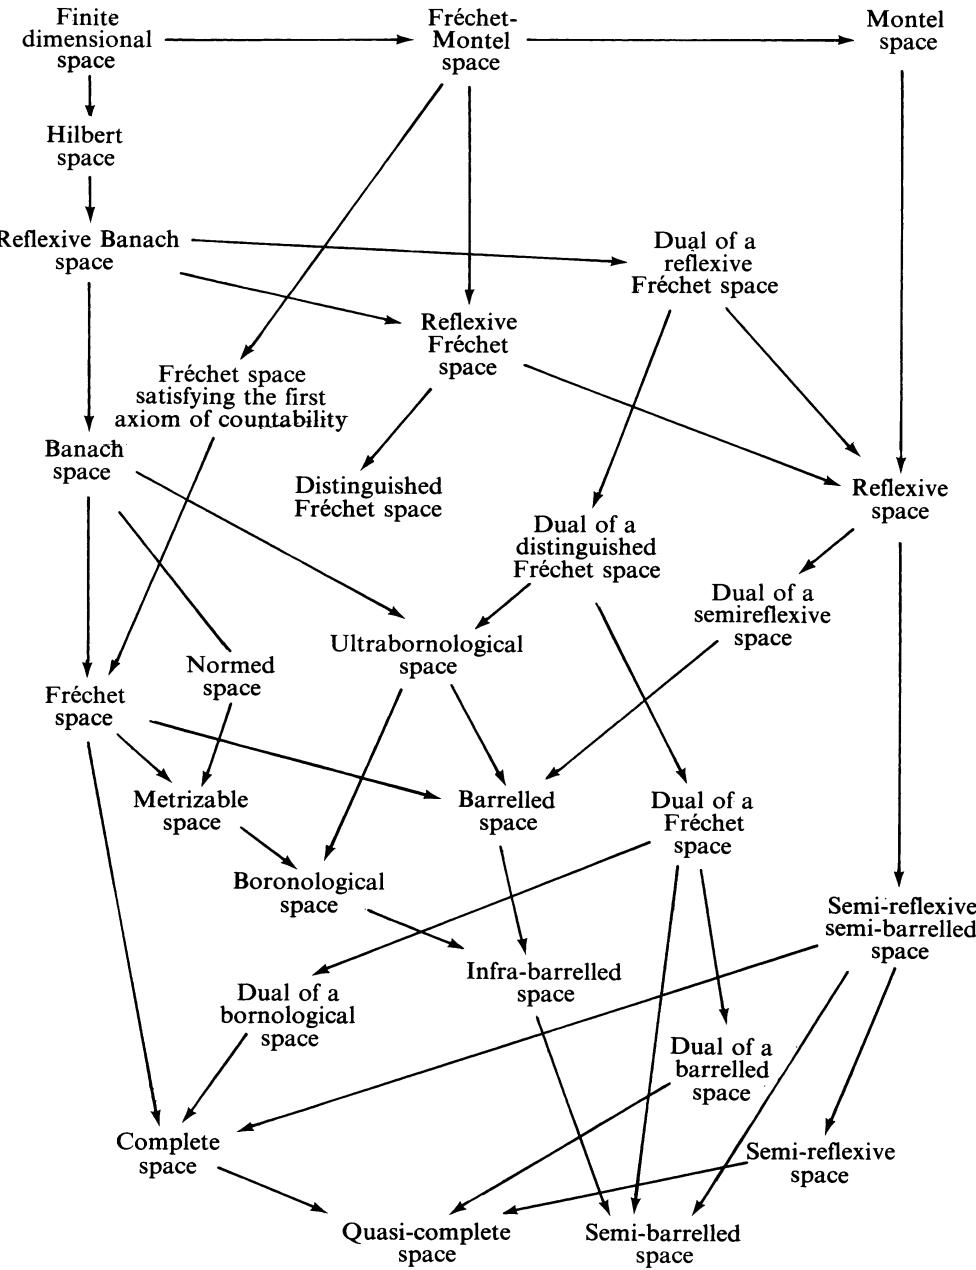
\includegraphics[keepaspectratio]{images/part002_27b26067.jpg}}

\bourbakitable{Principal bornologies on the dual of a locally convex space}{}
\pandocbounded{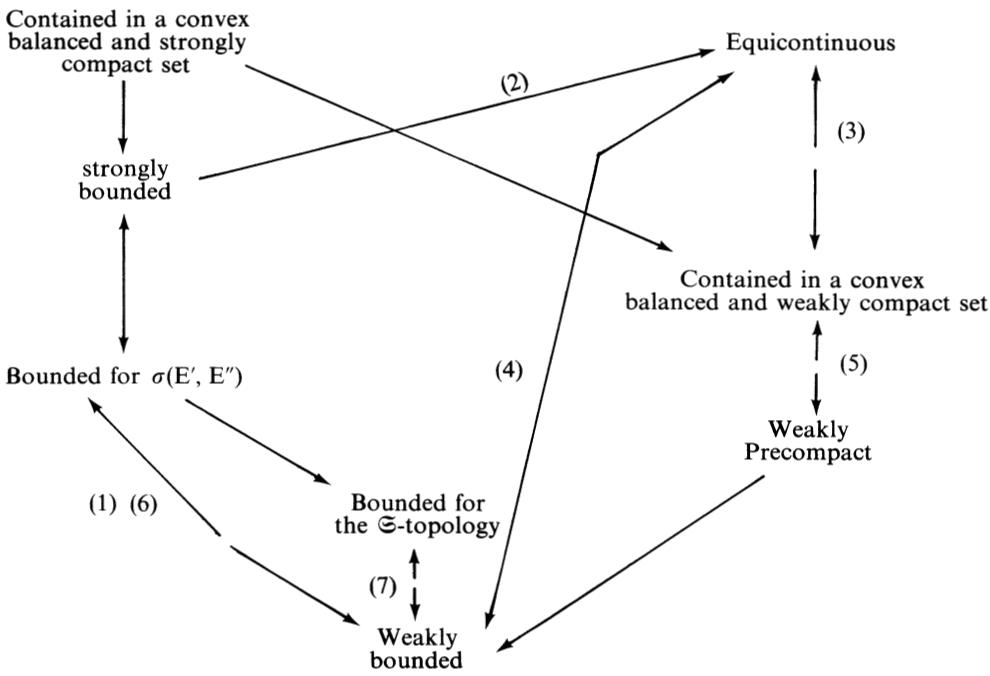
\includegraphics[keepaspectratio]{images/part002_d08e803b.jpg}}

N.B. --- We denote by S a family of bounded subsets of E such that every element is contained in a set belonging to S. A number on the side of an arrow indicates that the corresponding implication holds if the property with the same number is satisfied.

\paragraph{Properties}

\begin{enumerate}
\def\labelenumi{\arabic{enumi})}
\item
  Whenever E is semi-reflexive;
\item
  whenever E is bornological (III, p.~22, prop. 10);
\item
  if and only if E has the Mackey topology \(\tau(\mathrm{E},\mathrm{E}^{\prime})\) ;
\item
  if and only if E is barrelled;
\item
  if and only if \(\mathbf{E}'\) is quasi-complete for \(\sigma (\mathbf{E}',\mathbf{E})\)
\item
  whenever E is semi-complete (a fortiori, quasi-complete or complete) (III, p.~27, cor. 1);
\item
  whenever \(\mathfrak{S}\) consists of sets whose closed convex balanced envelope is semi-complete (III, p.~27, th. 2).
\end{enumerate}

When E is a Montel space, all the preceding bornologies are identical.

\chapter{\texorpdfstring{Hilbertian spaces \(^{1}\) (elementary theory)}{Hilbertian spaces \^{}\{1\} (elementary theory)}}

Throughout this chapter, K denotes the field R or the field C. For every complex number \(\xi = \alpha + i\beta (\alpha, \beta \text{ real}), \overline{\xi}\) denotes the conjugate \(\alpha - i\beta\) of \(\xi\) ; in particular, we have \(\overline{\xi} = \xi\) if and only if \(\xi\) is real.

\section{PREHILBERTIAN SPACES AND HILBERTIAN SPACES}

\subsection{Hermitian forms}

We recall the following definition given in Algebra (A, IX, § 3, No.~1):

DEFINITION 1. --- Let E be a vector space over the field K. A hermitian form (on the left) on E is a map f from E × E into K satisfying the following conditions (for \(x_{1}\) , \(x_{2}\) , x, \(y_{1}\) , \(y_{2}\) , y in E and \(\lambda\) , \(\mu\) in K):

\begin{enumerate}
\def\labelenumi{(\arabic{enumi})}
\tightlist
\item
\item
\end{enumerate}

\[
\begin{array}{c} \left\{ \begin{array}{l} f (x _ {1} + x _ {2}, y) = f (x _ {1}, y) + f (x _ {2}, y) \\ f (x, y _ {1} + y _ {2}) = f (x, y _ {1}) + f (x, y _ {2}) \end{array} \right. \\ \left\{ \begin{array}{l} f (\lambda x, y) = \overline {{\lambda}} f (x, y) \\ f (x, \mu y) = \mu f (x, y) \\ f (x, y) = \overline {{f (y , x)}}  . \end{array} \right. \end{array}\tag{3}
\]

When the field K is R, the notion of hermitian form on E reduces to that of symmetric bilinear form on \(E \times E\) (A, III, § 6, No.~3).

We note that the second condition (1) and the second condition (2) follow from the other three.

From (1) and (2) we deduce immediately that

\[
f \left(\sum_ {j} \lambda_ {j} x _ {j}, \sum_ {k} \mu_ {k} y _ {k}\right) = \sum_ {j, k} \bar {\lambda} _ {j} \mu_ {k} f \left(x _ {j}, y _ {k}\right).\tag{4}
\]

In particular, if \(\mathbf{E}\) is finite dimensional, and if \((e_j)_{1 \leqslant j \leqslant n}\) is a basis of \(\mathbf{E}\) , then for \(x = \sum_{j=1}^{n} \xi_j e_j\) and \(y = \sum_{j=1}^{n} \eta_j e_j\) , we have,

\[
f (x, y) = \sum_ {j, k} \alpha_ {j k} \overline {{{{\xi}}}} _ {j} \eta_ {k}
\]

with the notation \(\alpha_{jk} = f(e_j, e_k)\) ; moreover, relation (3) amounts to \(\alpha_{jk} = \overline{\alpha_{kj}}\) for every pair of indices \(j, k\) ; this implies in particular that the numbers \(\alpha_{jj}\) are real.

From (3), the number \(Q(x) = f(x, x)\) is real for all \(x \in E\) . Moreover, we immediately establish the following formulas, known as polarization formulas

\begin{enumerate}
\def\labelenumi{(\arabic{enumi})}
\setcounter{enumi}{4}
\tightlist
\item
\end{enumerate}

\[
4 f (x, y) = \sum_ {\varepsilon^ {2} = 1} \varepsilon \mathrm{Q} (x + \varepsilon y) \quad \text { if } \quad \mathbf {K} = \mathbf {R},\tag{6}
\]

\[
4 f (x, y) = \sum_ {\varepsilon^ {4} = 1, \varepsilon \in \mathbf {C}} \varepsilon \mathrm{Q} (x + \overline {{{\varepsilon}}} y) \quad \text { if } \quad \mathbf {K} = \mathbf {C}.
\]

Remark. --- We observe that formula (6) is valid for every sesquilinear form on \(E \times E\) (that is to say, for every function f satisfying (1) and (2), but not necessarily (3)). This remark shows that, when K = C, a sesquilinear form f such that \(f(x, x)\) is real for all \(x \in E\) is necessarily hermitian: relation (6) then gives \(\overline{f(y, x)} = f(x, y)\) since we have \(y + \varepsilon x = \varepsilon(x + \overline{\varepsilon}y)\) and \(\mathbf{Q}(\varepsilon z) = \mathbf{Q}(z)\) whenever \(\varepsilon^{4} = 1\) .

From the polarisation formulas, we have in particular,

PROPOSITION 1. --- If \(f\) is a hermitian form on \(\mathbf{E}\) , and \(\mathbf{M}\) a vector subspace of \(\mathbf{E}\) such that \(f(x, x) = 0\) for all \(x \in \mathbf{M}\) , then we also have \(f(x, y) = 0\) for every pair of points \(x, y\) in \(\mathbf{M}\) .

Let \(f\) be a hermitian form on \(\mathbf{E}\) ; the set \(\mathbf{N}\) of all \(x \in \mathbf{E}\) such that \(f(x, y) = 0\) for all \(y \in \mathbf{E}\) is a vector subspace of \(\mathbf{E}\) . It follows from (3) that, if \(x_1 \equiv x_2 \pmod{\mathbf{N}}\) and \(y_1 \equiv y_2 \pmod{\mathbf{N}}\) , we have \(f(x_1, y_1) = f(x_2, y_2)\) ; hence, on the quotient space \(\mathrm{E/N}\) we define a sesquilinear form \(f\) by putting \(\dot{f}(\dot{x}, \dot{y}) = f(x, y)\) for all \(x \in \dot{x}\) and all \(y \in \dot{y}\) ; it is clear that \(\dot{f}\) is hermitian and that the relation \(\langle \dot{f}(\dot{x}, \dot{y}) = 0 \text{ for all } \dot{y} \in \mathrm{E/N} \rangle\) implies \(\dot{x} = 0 \text{ in } \mathrm{E/N}\) , in other words (A, IX) \(\dot{f}\) is separating. We say that \(f\) is the separating hermitian form associated with \(f\) .

\subsection{Positive hermitian forms}

DEFINITION 2. --- Let E be a vector space over the field K. A hermitian form f on E is said to be positive if \(f(x, x) \geqslant 0\) for all \(x \in E\) .

It is clear that hermitian forms on a vector space E form a vector space over the field R (but not over the field C, when K is C): in this space the positive hermitian forms constitute a pointed convex proper cone (II, p.~10) as a result of def. 2 and prop. 1.

PROPOSITION 2. --- If \(f\) is a positive hermitian form, we have

\[
\left| f (x, y) \right| ^ {2} \leqslant f (x, x) f (y, y)\tag{7}
\]

for every x and y in E (Cauchy-Schwarz inequality).

First assume that we have \(f(y, y) \neq 0\) . For every \(\xi \in \mathbf{K}\) , we have

\[
f (y, y) f (x + \xi y, x + \xi y) \geqslant 0
\]

which can be written as

\[
f (x, x) f (y, y) - | f (x, y) | ^ {2} + (\xi f (y, y) + \overline {{f (x , y)}}) (\bar {\xi} f (y, y) + f (x, y)) \geqslant 0.
\]

Replacing \(\xi\) by \(-\overline{f(x,y)} / f(y,y)\) in this inequality, we get (7). If \(f(x,x)\neq 0\) , we argue similarly.

Finally, if \(f(x, x) = f(y, y) = 0\) , we have \(f(x + \xi y, x + \xi y) \geqslant 0\) for all \(\xi \in \mathbf{K}\) , which can be written as

\[
\xi f (x, y) + \overline {{{{\xi f (x , y)}}}} \geqslant 0.
\]

Replacing \(\xi\) by \(-\overline{f(x,y)}\) in this inequality, we get \(-2|f(x,y)|^2 \geqslant 0\) , and therefore \(f(x,y) = 0\) ; we again get (7) in this case.

COROLLARY 1. --- If \(f\) is a positive hermitian form, the set \(\mathbf{N}\) of all \(x \in \mathbf{E}\) such that \(f(x, x) = 0\) coincides with the vector subspace of all \(x \in \mathbf{E}\) such that \(f(x, y) = 0\) for all \(y \in \mathbf{E}\) .

COROLLARY 2. --- For a positive hermitian form to be separating, it is necessary and sufficient that the relation \(x \neq 0\) implies \(f(x, x) > 0\) .

This follows immediately from cor. 1.

For every positive hermitian form f on E, the separating hermitian form associated with \(f(\mathrm{V}, \mathrm{p.~2})\) is evidently a positive hermitian form on E/N.

PROPOSITION 3. --- Let f be a positive hermitian form on E. Put

\[
p (x) = f (x, x) ^ {1 / 2}
\]

for all \(x \in \mathbb{E}\) . Then \(p\) is a semi-norm on \(\mathbb{E}\) , and is a norm if and only if \(f\) is separating. It is enough to prove the inequality \(p(x + y) \leqslant p(x) + p(y)\) . But we have

\[
f (x + y, x + y) = f (x, x) + f (y, y) + f (x, y) + \overline {{f (x , y)}}
\]

and, by Cauchy-Schwarz inequality

\[
\begin{array}{c} f (x + y, x + y) \leqslant f (x, x) + f (y, y) + 2 (f (x, x) f (y, y)) ^ {1 / 2} \\ = \bigl (f (x, x) ^ {1 / 2} + f (y, y) ^ {1 / 2} \bigr) ^ {2}. \end{array}\tag{8}
\]

Remarks. --- 1) Suppose \(f\) is positive and separating, and let \(x, y\) be two vectors \(\neq 0\) . The proof of Cauchy-Schwarz inequality shows that, if the two members of (7) are equal, then there exists a scalar \(\xi\) such that \(f(x + \xi y, x + \xi y) = 0\) , hence \(x + \xi y = 0\) , in other words, x and y are linearly dependent; the converse is immediate. The proof of inequality (8) shows that the equality \(p(x + y) = p(x) + p(y)\) is possible only if x and y are linearly dependent; if \(y = \lambda x\) , the preceding equality can be written as \(|1 + \lambda| = 1 + |\lambda|\) , and implies that \(\lambda\) is real and positive.

\begin{enumerate}
\def\labelenumi{\arabic{enumi})}
\setcounter{enumi}{1}
\tightlist
\item
  Let \(f\) be a positive hermitian form on \(\mathbf{E}\) , and let \(\mathbf{E}\) be assigned the semi-norm \(x \mapsto f(x, x)^{1/2}\) ; if \(\dot{f}\) is the positive, separating hermitian form defined on \(\mathrm{E/N}\) associated with \(f\) , then the normed space obtained by assigning the norm \(x \mapsto \hat{f}(\dot{x}, \dot{x})^{1/2}\) to \(\mathrm{E/N}\) is the normed space associated with \(\mathbf{E}\) (II, p.~5).
\end{enumerate}

DEFINITION 3. --- Let E be a vector space over the field K. A semi-norm p on E is said to be prehilbertian if there exists a positive hermitian form f on E such that \(p(x) = f(x, x)^{1/2}\) for all \(x \in E\) .

Observe that for a semi-norm p on E, there exists at most one positive hermitian form f such that \(p(x) = f(x, x)^{1/2}\) for all \(x \in E\) ; this follows from the polarization formulas (V, p.~2).

\subsection{Prehilbertian spaces}

DEFINITION 4. --- A prehilbertian space is a set E with the structure of a vector space over K and with a positive hermitian form. We say that E is a real (resp. complex) prehilbertian space when K is R (resp. K is C).

Examples. --- 1) The form \((\lambda, \mu) \mapsto \overline{\lambda}\mu\) defines a prehilbertian structure on K, said to be canonical. When K is considered as a prehilbertian space, we shall always mean, unless otherwise mentioned that it has this structure.

\begin{enumerate}
\def\labelenumi{\arabic{enumi})}
\setcounter{enumi}{1}
\tightlist
\item
  Let I be an interval (bounded or not) in R, and let E be the set of regulated functions (FVR, II, p.~4) defined on I with values in C, having compact support. It is clear
\end{enumerate}

that \(\mathbf{E}\) is a vector space over \(\mathbf{C}\) ; let \(f\) be the sesquilinear form \((x, y) \mapsto \int_{1}^{\infty} \overline{x(t)} y(t) dt\) ;

it is immediate that \(f\) is a positive hermitian form on \(E\) , and hence defines a prehilbertian structure on this space.

\begin{enumerate}
\def\labelenumi{\arabic{enumi})}
\setcounter{enumi}{2}
\tightlist
\item
  Let \(n \geqslant 0\) be an integer. We define a prehilbertian space structure on the space \(\mathbf{K}^n\) , by means of the hermitian form
\end{enumerate}

\[
(x, y) \mapsto \sum_ {j = 1} ^ {n} \overline {{{{x}}}} _ {j} y _ {j}
\]

(for \(x = (x_{1}, \ldots, x_{n})\) and \(y = (y_{1}, \ldots, y_{n})\) ). When \(\mathbf{K}\) is \(\mathbf{R}\) , we see that this is just the scalar product of two vectors of \(\mathbf{R}^{n}\) (GT, VI, § 2, No.~2).

* 4) Let \(\ell^2\) (or \(\ell^2(\mathbf{N})\) ) be the set of sequences \(x = (x_n)_{n \in \mathbb{N}}\) of elements of \(\mathbf{K}\) such that \(\sum_{n=0}^{\infty} |x_n|^2\) is finite. One can show that \(\ell^2\) is a vector subspace of \(\mathbf{K}^{\mathbf{N}}\) and define a pre-

hilbertian space structure on \(\ell^2\) by means of the hermitian form \((x, y) \mapsto \sum_{n=0}^{\infty} \overline{x}_n y_n\) (cf.~V, p.~18).

\begin{enumerate}
\def\labelenumi{\arabic{enumi})}
\setcounter{enumi}{4}
\tightlist
\item
  Let \(\mathbf{E}\) be a real prehilbertian space, \(f\) the corresponding symmetric bilinear form on \(\mathbf{E}\) . Let \(\mathrm{E}_{(\mathbf{C})}\) be the vector space complexification of \(\mathbf{E}\) ; we identify \(\mathbf{E}\) with a subset of \(\mathrm{E}_{(\mathbf{C})}\) by the map \(x \mapsto 1 \otimes x\) , in such a way that every element of \(\mathrm{E}_{(\mathbf{C})}\) can be written uniquely as \(x_1 + ix_2\) with \(x_1, x_2\) in \(\mathbf{E}\) . The map \(f\) extends uniquely to a hermitian form \(f_{(\mathbf{C})}\) on \(\mathrm{E}_{(\mathbf{C})}\) ; we have,
\end{enumerate}

\[
f _ {(\mathbf {C})} \left(x _ {1} + i x _ {2}, y _ {1} + i y _ {2}\right) = f \left(x _ {1}, y _ {1}\right) + f \left(x _ {2}, y _ {2}\right) + i \left(f \left(x _ {1}, y _ {2}\right) - f \left(x _ {2}, y _ {1}\right)\right).
\]

In particular, we have

\[
f _ {(\mathbf {C})} (x _ {1} + i x _ {2}, x _ {1} + i x _ {2}) = f (x _ {1}, x _ {1}) + f (x _ {2}, x _ {2}) \geqslant 0,
\]

hence \(f_{(\mathbf{C})}\) is positive. We say that \(\mathrm{E}_{(\mathbf{C})}\) , with \(f_{(\mathbf{C})}\) is the prehilbertian space complexification of \(\mathbf{E}\) .

Whenever only one prehilbertian space structure on a vector space E is under consideration, the value, for a pair \((x, y)\) of points of E, of the hermitian form which defines the said structure is denoted by \(\langle x|y\rangle_{E}\) or simply \(\langle x|y\rangle\) , if no confusion is likely to arise. This number is called the scalar product \(^{1}\) of x and y (scalar square of x if y = x). Two vectors x, y are said to be orthogonal if \(\langle x|y\rangle = 0\) . The function \(x \mapsto \|x\| = \langle x|x\rangle^{1/2}\) is a semi-norm on the vector space E (V, p.~3); a prehilbertian space is always considered with this semi-norm assigned to it (and consequently also with the corresponding topology and uniform structure).

With these notations, in a prehilbertian space E, the Cauchy-Schwarz inequality can be written as

\[
\left| \langle x | y \rangle \right| \leqslant \| x \|\cdot \| y \|.\tag{9}
\]

Consequently, the scalar product is a continuous sesquilinear form on \(\mathbf{E} \times \mathbf{E}\) (II, p.~5, prop. 4).

In order that E be Hausdorff, it is necessary and sufficient that \(x \mapsto \|x\|\) is a norm on E; in other words, that the hermitian form \((x, y) \mapsto \langle x | y \rangle\) is positive and separating; this is equivalent to saying that 0 is the only vector of E, which is orthogonal to itself.

According to general definitions (S, IV, § 1, No.~5), an isomorphism from a prehilbertian space E onto a prehilbertian space F is a bijective linear mapping u from E onto F such that

\[
\langle u (x) | u (y) \rangle = \langle x | y \rangle\tag{10}
\]

for every x and y in E. We deduce from this that \(\|u(x)\| = \|x\|\) for all \(x \in E\) , and u is evidently an isomorphism for the topological vector space structures of E and of F; if E and F are Hausdorff, u is an isometry from E onto F. Conversely, if u is a bijective linear mapping from E onto F, such that \(\|u(x)\| = \|x\|\) for all \(x \in E\) , the polarization formulas (V, p.~2) show that u is a prehilbertian space isomorphism from E onto F.

Let \(E\) be a complex prehilbertian space, and \(\langle x|y\rangle\) the scalar product in \(E\) . On the set \(E\) , we can define a second vector space structure with respect to \(C\) , taking the same law of the additive group and for the law of external composition \((\lambda, x) \mapsto \overline{\lambda}x\) (A, II, § 1, No.~13) for this vector space structure, \((x, y) \mapsto \langle y|x\rangle\) is a positive hermitian

\(^{1}\) It may happen sometimes that we write \((x|y)\) for \(\langle y|x\rangle\) . Observe that the formula (4) of V, p.~2, takes the following equivalent forms:

(4')

\[
\langle \sum_ {i} \lambda_ {i} x _ {i} | \sum_ {j} \mu_ {j} y _ {j} \rangle = \sum_ {i, j} \overline {{{{\lambda}}}} _ {i} \mu_ {j} \langle x _ {i} | y _ {j} \rangle .\tag{4"}
\]

\[
(\sum_ {i} \lambda_ {i} x _ {i} | \sum_ {j} \mu_ {j} y _ {j}) = \sum_ {i, j} \lambda_ {i} \overline {{\mu}} _ {j} (x _ {i} | y _ {j}).
\]

form. The prehilbertian space \(\overline{E}\) obtained by assigning this new vector space structure and the new hermitian form to E, is said to be conjugate to E. An isomorphism u from E onto \(\overline{E}\) is a semi-linear mapping from E onto itself (with respect to the automorphism \(\xi \mapsto \overline{\xi}\) of C) such that \(\langle u(y)|u(x)\rangle = \langle x|y\rangle\) or \(\langle u(x)|u(y)\rangle = \overline{\langle x|y\rangle}\) (for x, y in E); such a mapping is said to be a semi-automorphism of the prehilbertian space E.

If E is a prehilbertian space, M a vector subspace of E, the restriction of the scalar product \(\langle x|y\rangle\) to \(M \times M\) is a positive hermitian form on M, which then defines a prehilbertian space structure on M; we say that this structure is induced by the structure of E, or that M is a prehilbertian subspace of E.

\subsection{Hilbertian spaces}

DEFINITION 5. --- A hilbertian space (or Hilbert space) is a prehilbertian space which is Hausdorff and complete. We say that a norm on a vector space E (over K) is hilbertian if it is prehilbertian, and if the normed space E is complete.

If E is a hilbertian space and M a closed vector subspace of E, the prehilbertian space structure induced on M is in fact a hilbertian space structure. In this case we say that M, with the induced structure is a hilbertian subspace of E.

Examples. --- 1) The prehilbertian spaces defined in examples 1, 3, 4 of V, p.~4, are hilbertian spaces. On the other hand, the prehilbertian space defined in example 2 is neither Hausdorff, nor complete. The complexification of a hilbertian space is a hilbertian space.

* 2) Let X be a Hausdorff topological space and let \(\mu\) be a positive measure on X. Let \(L^2(X, \mu)\) be the space consisting of equivalence classes, for \(\mu\) , of all square \(\mu\) -integrable functions on X with values in C. This is a complex hilbertian space, whose scalar product is given by

\[
\langle f | g \rangle = \int_ {\mathrm{X}} \overline {{{f (x)}}} g (x) d \mu (x). *
\]

* 3) Let \(n \geqslant 1\) be an integer and let \(U\) be an open set in \(\mathbf{R}^n\) . Let \(\mu\) be the measure on \(U\) induced by the Lebesgue measure on \(\mathbf{R}^n\) , and put \(\mathcal{H}^0 = L^2(U, \mu)\) . Let \(\mathcal{H}^1\) denote the space of all functions \(f \in \mathcal{H}^0\) with the following property; for \(1 \leqslant i \leqslant n\) , there exists a function \(g_i \in \mathcal{H}^0\) such that

\[
\int_ {\mathrm{U}} g _ {i} (x) h (x) d \mu (x) = - \int_ {\mathrm{U}} f (x) \mathrm{D} _ {i} h (x) d \mu (x)
\]

for every function \(h\) of class \(\mathbf{C}^1\) with compact support in \(\mathbf{U}\) . The function \(g_i\) is defined uniquely up to equivalence with respect to \(\mu\) , and is denoted by \(\mathbf{D}_i f\) or \(\partial f / \partial x_i\) (ith partial derivative). By induction on the integer \(s \geqslant 1\) , we define \(\mathcal{H}^s\) as the set of all functions \(f \in \mathcal{H}^1\) such that \(D_i f \in \mathcal{H}^{s-1}\) for \(1 \leqslant i \leqslant n\) . We define a scalar product on \(\mathcal{H}^s\) by the formula

\[
\langle f | g \rangle = \sum_ {k = 0} ^ {s} \sum_ {1 \leqslant i _ {1} \leqslant \dots \leqslant i _ {k} \leqslant n} \int \overline {{{{\mathrm{D} _ {i _ {1}} \dots \mathrm{D} _ {i _ {k}} f}}}}. \mathrm{D} _ {i _ {1}} \dots \mathrm{D} _ {i _ {k}} g d \mu .
\]

Then \(\mathcal{H}^s\) is a complex hilbertian space, called Sobolev space of index \(s\) .

* 4) Let X be a differential variety of class \(\mathbf{C}^r\) (with \(r \geqslant 1\) ) pure of finite dimension \(n\) .

In the vector fibre space \(\Lambda^{n}\mathrm{T}(\mathrm{X})\) , let L be the complement of the zero section. For every real number \(\lambda \neq 0\) , the mapping \(u \mapsto \lambda u\) from \(\Lambda^{n}\mathrm{T}(\mathrm{X})\) into itself leaves L stable.

Let \(\alpha\) be a complex number. A complex valued function \(\omega\) on \(\mathbf{L}\) such that \(\omega (\lambda u) = |\lambda |^{\alpha}\omega (u)\) for \(u\in \mathbf{L}\) and any non-zero real number \(\lambda\) is called a density of order \(\alpha\) on \(\mathbf{X}\) . We say that a density \(\omega\) of order 1 is locally integrable if there exists an open cover \((\mathrm{U}_i)_{i\in \mathbf{I}}\) of \(\mathbf{X}\) , and for every \(i\in \mathbf{I}\) a system of coordinates \(\xi_i = (\xi_i^1,\dots,\xi_i^n)\) on \(\mathrm{U}_i\) and a complex valued function \(f_{i}\) on \(\xi_i(\mathrm{U}_i)\) satisfying the following conditions: a) The function \(f_{i}\) is locally integrable on the open set \(\xi_i(\mathrm{U}_i)\) of \(\mathbf{R}^n\) with respect to the Lebesgue measure \(\mu\) ;

\begin{enumerate}
\def\labelenumi{\alph{enumi})}
\setcounter{enumi}{1}
\tightlist
\item
  Let \(x \in \mathbf{U}_i\) ; if \((\partial_{1,i,x}, \ldots, \partial_{n,i,x})\) is the basis of \(\mathrm{T}_x\mathrm{X}\) associated to the system of coordinates \((\xi_i^1, \ldots, \xi_i^n)\) in \(\mathbf{U}_i\) we have
\end{enumerate}

\[
\omega \left(\partial_ {1, i, x} \wedge \dots \wedge \partial_ {n, i, x}\right) = f _ {i} \left(\xi_ {i} ^ {1} (x), \dots , \xi_ {i} ^ {n} (x)\right).
\]

Then, there exists one and only one measure \(\tilde{\omega}\) on \(\mathbf{X}\) such that for every \(i\in \mathrm{I}\) , the image under \(\xi_{i}\) of the restriction of \(\tilde{\omega}\) to \(\mathrm{U}_i\) is equal to the measure \(f_{i}.\mu\) (cf.~VAR, R, 10.4.3).

Let \(\mathcal{V}\) (resp. \(\mathcal{N}\) ) be the vector space of measurable densities \(\omega\) of order \(1/2\) such that the measure associated with the density \(|\omega|^2\) of order 1 is bounded (resp. null). Let \(\omega_1\) and \(\omega_2\) be in \(\mathcal{V}\) ; then \(\omega = \overline{\omega}_1\omega_2\) is a density of order 1, and the measure \(\tilde{\omega}\) associated with \(\omega\) is bounded; the number \(\int_{\mathbf{X}}\tilde{\omega}\) depends only on the classes \(\dot{\omega}_1\) and \(\dot{\omega}_2\) of \(\omega_1\) and \(\omega_2\) modulo \(\mathcal{N}\) and is denoted by \(\langle\omega_1|\omega_2\rangle\) or \(\langle\dot{\omega}_1|\dot{\omega}_2\rangle\) . Then the mapping \((\dot{\omega}_1,\dot{\omega}_2)\mapsto\langle\dot{\omega}_1|\dot{\omega}_2\rangle\) assigns a complex hilbertian space structure to the vector space \(\Omega_{1/2}(\mathbf{X})=\mathcal{V}/\mathcal{N}_{*}\) .

*5) Let D be the open disc with centre 0 and radius 1 in C. The Hardy space \(\mathrm{H}^2 (\mathbf{D})\) consists of all holomorphic functions \(f\colon \mathbf{D}\to \mathbf{C}\) for which

\[
\sup _ {0 <   \mathbf {R} <   1} \int_ {0} ^ {1} | f (\mathbf {R}. \mathbf {e} (\theta)) | ^ {2} d \theta <   + \infty .
\]

If \(f_{1}\) and \(f_{2}\) belong to \(\mathrm{H}^2 (\mathbf{D})\) , the limit

\[
\langle f _ {1} | f _ {2} \rangle = \lim _ {\mathbf {R} \rightarrow 1} \int_ {0} ^ {1} \overline {{{f _ {1} (\mathbf {R} . \mathbf {e} (\theta))}}}. f _ {2} (\mathbf {R}. \mathbf {e} (\theta)) d \theta
\]

exists; the mapping \((f_1, f_2) \mapsto \langle f_1 | f_2 \rangle\) assigns a complex hilbertian space structure to the vector space \(\mathbf{H}^2(\mathbf{D})\) .

For a function \(f: \mathbf{D} \to \mathbf{C}\) to belong to \(\mathbf{H}^2(\mathbf{D})\) , it is necessary and sufficient that there exists a sequence \((a_n)_{n \in \mathbb{N}}\) of complex numbers such that \(\sum_{n=0}^{\infty} |a_n|^2 < +\infty\) and that

\[
f (z) = \sum_ {n = 0} ^ {\infty} a _ {n} z ^ {n}
\]

for all \(z \in \mathbf{D}\) . Then we have \(\| f\|^2 = \sum_{n=0}^{\infty} |a_n|^2\) which gives an isomorphism from \(\mathrm{H}^2(\mathrm{D})\) onto the hilbertian space \(\ell^2\) (V, p.~4). *

Every Hausdorff prehilbertian space is isomorphic to an everywhere dense subspace of a hilbertian space determined up to an isomorphism. Precisely :

PROPOSITION 4. --- Let E be a Hausdorff prehilbertian space, \(\hat{E}\) the normed space completion of E(GT, IX, § 3, No.~3). The scalar product \((x, y) \mapsto \langle x|y \rangle\) extends by continuity to a positive and separating hermitian form on \(\hat{\mathbf{E}}\) , and defines a hilbertian space structure on \(\hat{\mathbf{E}}\) .

The existence of the extension of \((x, y) \mapsto \langle x|y \rangle\) to \(\hat{E} \times \hat{E}\) follows from the continuity of this sesquilinear form on \(E \times E\) (GT, III, §6, No.~5, th. 1). Moreover, this extension, which will also be denoted by \((x, y) \mapsto \langle x|y \rangle\) is a hermitian form and satisfies the relation \(\langle x|x\rangle = \|x\|^2\) , by virtue of the principle of extension of identities ( \(\|x\|\) being the norm on \(\hat{E}\) obtained by extending the norm on E by continuity); this proves that the relation \(\langle x|x\rangle = 0\) implies x = 0 in \(\hat{E}\) , hence that the form \((x, y) \mapsto \langle x|y \rangle\) is positive and separating, and consequently defines a hilbertian space structure on \(\hat{E}\) .

Q.E.D.

This hilbertian space is said to be the completion of the Hausdorff prehilbertian space E.

* Example 6. --- Let U be an open subset of \(\mathbf{R}^n\) ( \(n \geqslant 1\) ). Let \(\mathcal{C}_0^1(\mathrm{U})\) be the vector space of all functions of class \(\mathbf{C}^1\) with compact support in U. We define a Hausdorff prehilbertian space structure on \(\mathcal{C}_0^1(\mathrm{U})\) whose scalar product is given by

\[
\langle f | g \rangle = \sum_ {i = 1} ^ {n} \int_ {\mathrm{U}} \overline {{{{\mathbf {D} _ {i} f (x)}}}}. \mathbf {D} _ {i} g (x) d x.
\]

This prehilbertian space is not complete. Its completion is called the Dirichlet space associated with U. *

COROLLARY. --- Let V be a vector space over K and f a positive hermitian form on V. a) There exists a Hilbert space E and a linear mapping \(u:V \rightarrow E\) such that \(f(x,y) = \langle u(x)|u(y) \rangle\) for x, y in V, and such that \(u(V)\) is dense in E.

\begin{enumerate}
\def\labelenumi{\alph{enumi})}
\setcounter{enumi}{1}
\tightlist
\item
  If two pairs \((\mathbf{E}_{i}, u_{i})\) satisfy the conditions analogous to a), then there exists a unique isomorphism \(\phi\) from the Hilbert space \(E_{1}\) onto the Hilbert space \(E_{2}\) such that \(u_{2} = \phi \circ u_{1}\) .
\end{enumerate}

Let N be the set of all \(x \in V\) such that \(f(x, x) = 0\) . We define a positive and separating hermitian form on the space V/N by \(\langle \dot{x} | \dot{y} \rangle = f(x, y)\) for \(x \in \dot{x}\) and \(y \in \dot{y}\) . Let E be the hilbertian space completion of V/N and u the mapping \(x \mapsto x + N\) from V into E. Then the conditions of a) are satisfied.

Under the hypotheses of b), N is equal to the kernel of \(u_{1}\) and to that of \(u_{2}\) . Hence there exists a bijective linear mapping \(\phi_{0}\) from \(u_{1}(V)\) onto \(u_{2}(V)\) such that \(u_{2}(x) = \phi_{0}(u_{1}(x))\) for all \(x \in V\) . We verify immediately that \(\phi_{0}\) is an isomorphism of prehilbertian spaces, hence an isometry. Since \(u_{i}(V)\) is dense in \(E_{i}\) for i = 1, 2, \(\phi_{0}\) extends uniquely to an isometry \(\phi\) from \(E_{1}\) onto \(E_{2}\) , and b) follows.

We say that the hilbertian space \(\mathbf{E}\) is the separated completion of \(\mathbf{V}\) (for the form \(f\) ).

Example 7. --- Let G be a group (with unit element 1) and \(\pi\) a homomorphism from G into the group of automorphisms of a complex hilbertian space E; we say that \(\pi\) is a unitary representation of G in E. Let \(a \in E\) ; we put

\[
\phi (x) = \langle a | \pi (x). a \rangle
\]

for all \(x \in \mathbf{G}\) . Then \(\phi : \mathbf{G} \to \mathbf{C}\) is positive definite, in other words satisfies the relation :

(PD) For every \(\lambda_{1},\ldots,\lambda_{n}\) in C and \(x_{1},\ldots,x_{n}\) in G, we have

\[
\sum_ {i, j = 1} ^ {n} \overline {{\lambda}} _ {i} \lambda_ {j} \phi (x _ {i} ^ {- 1} x _ {j}) \geqslant 0.\tag{11}
\]

In fact, the first member of (11) is precisely \(\| \sum_{i=1}^{n} \lambda_i \pi(x_i). a \|^2\) .

Conversely, let \(\phi\) be a positive definite function on \(G\) . Let \(\mathbf{C}^{(G)}\) be the vector space of all functions with finite support on \(G\) . We define a hermitian form \(\Phi\) on \(G\) by

\[
\Phi (u, v) = \sum_ {x, y \in G} \overline {{u (x)}} v (y) \phi (x ^ {- 1} y)\tag{12}
\]

and the relation (PD) expresses the fact that \(\Phi\) is positive. By the corollary of prop. 4, there exists a hilbertian space \(E\) and a linear mapping \(\rho : \mathbf{C}^{(G)} \to E\) , with a dense image, such that

\[
\Phi (u, v) = \langle \rho (u) | \rho (v) \rangle \quad \text { for } \quad u, v \quad \text { in } \quad \mathbf {C} ^ {(G)}.\tag{13}
\]

For every \(x \in \mathbf{G}\) , let \(\gamma_x\) be the left translation by \(x\) in \(\mathbf{C}^{(\mathrm{G})}\) defined by \(\gamma_x u(y) = u(x^{-1}y)\) for \(u \in \mathbf{C}^{(\mathrm{G})}\) and \(y \in \mathbf{G}\) . We have \(\Phi(\gamma_x u, \gamma_x v) = \Phi(u, v)\) . Now apply assertion \(b\) of the corollary of prop. 4 to \(\rho\) and \(\rho \circ \gamma_x\) : there exists a unique automorphism \(\pi(x)\) of the hilbertian space \(E\) such that \(\rho \circ \gamma_x = \pi(x) \circ \rho\) . We see immediately that \(\pi\) is a homomorphism from \(G\) into the group of automorphisms of \(E\) .

Let \(\delta\) be the element of \(\mathbf{C}^{(\mathrm{G})}\) defined by \(\delta(1) = 1\) , \(\delta(x) = 0\) for \(x \neq 1\) in \(\mathbf{G}\) . We have \(u = \sum_{x \in \mathbf{G}} u(x) \cdot \gamma_x \delta\) for all \(u \in \mathbf{C}^{(\mathrm{G})}\) , and so \(\rho(u) = \sum_{x \in \mathbf{G}} u(x) \pi(x) \cdot a\) by putting \(a = \rho(\delta)\) . Formulas (12) and (13) imply that \(\phi(x) = \langle a | \pi(x) \cdot a \rangle\) for all \(x \in \mathbf{G}\) . We remark that the set of vectors \(\pi(x) \cdot a\) for all \(x \in \mathbf{G}\) , is total in \(\mathbf{E}\) .

\subsection{Convex subsets of a prehilbertian space}

If we calculate \(\|x - y\|^{2} = \langle x - y|x - y \rangle\) and \(\|x + y\|^{2} = \langle x + y|x + y \rangle\) for any two points x, y of a prehilbertian space E, we immediately get the « identity of the median »

\[
\left\| \frac {1}{2} (x + y) \right\| ^ {2} + \left\| \frac {1}{2} (x - y) \right\| ^ {2} = \frac {1}{2} (\| x \| ^ {2} + \| y \| ^ {2}).\tag{14}
\]

From this identity we deduce the following proposition :

\pandocbounded{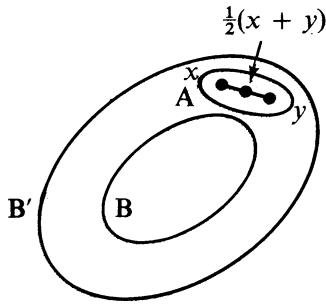
\includegraphics[keepaspectratio]{images/part002_56de9e6b.jpg}}\\
FIG. 1.

PROPOSITION 5. --- Let E be a prehilbertian space. Let d be a real number \textgreater0, δ a real number such that \(0 \leqslant \delta \leqslant d\) . Let B and B' be subsets of E defined by \(\|x\| < d\) , \(\| x\| \leqslant d + \delta\) respectively, and let A be a convex set contained in \(\mathbf{B}' - \mathbf{B}\) . Then for every pair of points \(x, y\) of A, we have \(\| x - y\| \leqslant \sqrt{12d\delta}\) (fig.~1).

In fact, we have \(\frac{1}{2} (x + y)\in \mathbf{A}\) , hence \(\| \frac{1}{2} (x + y)\| \geqslant d\) ; hence from (14) we get the inequality

\[
\left\| \frac {1}{2} (x - y) \right\| ^ {2} = \frac {1}{2} \left(\| x \| ^ {2} + \| y \| ^ {2}\right) - \left\| \frac {1}{2} (x + y) \right\| ^ {2} \leqslant (d + \delta) ^ {2} - d ^ {2} \leqslant 3 d \delta
\]

from which the proposition follows.

THEOREM 1. --- Let E be a prehilbertian space, and H a non-empty convex subset of E such that H is a Hausdorff and complete uniform subspace of E. For every \(x \in E\) , there exists a unique point \(p_{\mathrm{H}}(x)\) in H such that \(\|x - p_{\mathrm{H}}(x)\| = \inf_{y \in \mathrm{H}} \|x - y\|\) . The element \(p_{\mathrm{H}}(x)\) of H is also the unique element a of H satisfying the relation \(^{1}\)

\[
\mathcal {R} \langle x - a | y - a \rangle \leqslant 0\tag{15}
\]

for all \(y \in \mathbf{H}\) .

\pandocbounded{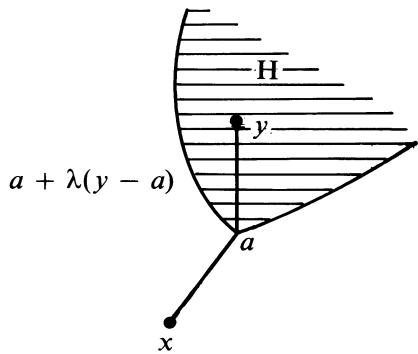
\includegraphics[keepaspectratio]{images/part002_6909685c.jpg}}\\
FIG. 2.

Put \(d = \inf_{y \in \mathbf{H}} \| x - y \|\) , and for every integer \(n > 0\) , let \(\mathrm{H}_n\) be the set of points \(y\) of \(\mathbf{H}\) such that \(\| x - y \| \leqslant d + n^{-1}\) . The set \(\mathrm{H}_n\) is closed in \(\mathbf{H}\) , is convex and non-empty, and its diameter is bounded by \(\sqrt{12d / n}\) for all large enough \(n\) , by prop. 5. The sequence \((\mathrm{H}_n)_{n \geqslant 1}\) being decreasing, and the set \(\mathbf{H}\) being Hausdorff and complete it follows that the base of the Cauchy filter \((\mathrm{H}_n)_{n \geqslant 1}\) converges to a point \(p_{\mathbf{H}}(x)\) of \(\mathbf{H}\) ; we have \(\{p_{\mathbf{H}}(x)\} = \bigcap_{n \geqslant 1} \mathrm{H}_n\) , hence \(p_{\mathbf{H}}(x)\) is the unique point \(a\) of \(\mathbf{H}\) such that \(\| x - a \| = d\) .

\(^{1}\) We recall (GT, VIII, § 1, No.~1) that \(\mathcal{R}(z)\) denotes the real part of the complex number z; we have \(\mathcal{R}(z)=z\) if z is real.

Let \(y \in H\) ; since \(H\) is convex, the point \(z(\lambda) = p_{\mathbf{H}}(x) + \lambda(y - p_{\mathbf{H}}(x))\) of \(E\) belongs to \(H\) for every real number \(\lambda\) such that \(0 < \lambda < 1\) . Hence we have

\[
\left\| x - z (\lambda) \right\| ^ {2} \geqslant \left\| x - p _ {\mathrm{H}} (x) \right\| ^ {2} \quad \text { for } \quad 0 <   \lambda <   1,
\]

which gives

\[
\mathcal {R} \left\langle x - p _ {\mathrm{H}} (x) \mid y - p _ {\mathrm{H}} (x) \right\rangle = \lim _ {\lambda \rightarrow 0} \frac {1}{2 \lambda} \left\{\| x - p _ {\mathrm{H}} (x) \| ^ {2} - \| x - z (\lambda) \| ^ {2} \right\} \leqslant 0.
\]

Conversely, let \(a\) be a point of \(\mathbf{H}\) such that \(\mathcal{R}\langle x - a|y - a\rangle \leqslant 0\) for all \(y\in \mathbf{H}\) . For every \(y\in \mathbf{H}\) , we have

\[
\left\| x - y \right\| ^ {2} = \left\| x - a \right\| ^ {2} + \left\| y - a \right\| ^ {2} - 2 \mathcal {R} \langle x - a | y - a \rangle \geqslant \left\| x - a \right\| ^ {2},
\]

and so \(\| x - a\| = d\) and finally that \(a = p_{\mathrm{H}}(x)\) follows from the first part of the proof. Q.E.D.

In what follows the mapping \(p_{H}\) of E in H will be called the projection from E onto H. We remark that \(p_{\mathrm{H}}(x)=x\) for all \(x\in H\) .

The first part of th. 1 is valid under more general hypotheses on the space E (V, p.~67, exerc. 31).

The proof of th. 1 establishes, among others, the following property :

COROLLARY 1. --- Let I be a set directed by a filter \(\mathfrak{F}\) and let \((y_i)_{i\in I}\) be a family of points of H. Let \(x\in E\) . Suppose that we have

\[
\lim _ {i, \mathfrak {F}} \| x - y _ {i} \| = \inf _ {z \in \mathrm{H}} \| x - z \|.
\]

Then \(y_{i}\) tends to \(p_{\mathrm{H}}(x)\) with respect to the filter \(\mathfrak{F}\) .

COROLLARY 2. --- For every x, y in E, we have

\[
\left\| p _ {\mathrm{H}} (x) - p _ {\mathrm{H}} (y) \right\| \leqslant \left\| x - y \right\|.
\]

In particular, the mapping \(p_{H}\) from E into H is continuous.

Let \(x, y\) be two points of \(E\) . Put \(a = p_{\mathrm{H}}(x) - x\) , \(b = p_{\mathrm{H}}(y) - p_{\mathrm{H}}(x)\) , \(c = y - p_{\mathrm{H}}(y)\) . By formula (15) (V, p.~10) we have \(\mathcal{R}\langle a|b\rangle \geqslant 0\) and \(\mathcal{R}\langle c|b\rangle \geqslant 0\) . We also have \(a + b + c = y - x\) , which gives,

\[
\| x - y \| ^ {2} = \| a + b + c \| ^ {2} = \| b \| ^ {2} + \| a + c \| ^ {2} + 2 \mathscr {R} \langle a | b \rangle + 2 \mathscr {R} \langle c | b \rangle
\]

\[
\geqslant \| b \| ^ {2} = \left\| p _ {\mathrm{H}} (x) - p _ {\mathrm{H}} (y) \right\| ^ {2}.
\]

This proves corollary 2.

PROPOSITION 6. --- Let E be a prehilbertian space and let \(\Phi\) be a non-empty, directed decreasing set of non-empty Hausdorff and complete convex subsets of E. For every \(x \in \mathrm{E}\) and every subset H of E, put \(d(x, \mathrm{H}) = \inf_{z \in \mathrm{H}} \| x - z \|\) . In order that the intersection M of the sets H belonging to \(\Phi\) be non-empty, it is necessary and sufficient that there exists \(x_0\) in E such that \(\sup_{\mathbf{H} \in \Phi} d(x_0, \mathbf{H})\) is finite. For every \(x \in \mathbf{E}\) we then have

\(p_{\mathbf{M}}(x) = \lim_{\mathrm{H}\in \Phi}p_{\mathrm{H}}(x)\) (limit with respect to the directed set \(\Phi\) ).

If \(\mathbf{M}\) is non-empty, \(d(x,\mathrm{H})\leqslant d(x,\mathbf{M})\) for all \(\mathbf{H}\in \Phi\) and all \(x\in \mathbb{E}\) .

Conversely, suppose that there exists a point \(x_0\) in \(\mathbf{E}\) and a real number \(\mathbf{C} \geqslant 0\) such that \(d(x_0, \mathbf{H}) \leqslant \mathbf{C}\) for all \(\mathbf{H} \in \Phi\) . Let \(x \in \mathbf{E}\) ; then

\[
d (x, \mathrm{H}) \leqslant \| x - x _ {0} \| + \mathrm{C} \quad \text { for   all } \quad \mathrm{H} \in \Phi ,
\]

hence the number \(d = \sup_{\mathbf{H} \in \Phi} d(x, \mathbf{H})\) is finite. Let \(\mathbf{B}\) be the set of all \(z \in E\) such that \(\| x - z\| \leqslant d\) . Since \(\mathbf{B}\) is convex and closed in \(\mathbf{E}\) , the sets \(\mathrm{H} \cap \mathrm{B}\) , for \(\mathrm{H}\) ranging over \(\Phi\) , are convex, Hausdorff and complete. Let \(\varepsilon > 0\) ; there exists a set \(\mathrm{H} \in \Phi\) such that \(d(x, \mathrm{H}) \geqslant \mathrm{d} - \varepsilon\) , and if \(\varepsilon < d/2\) , the diameter of \(\mathrm{H} \cap \mathrm{B}\) is bounded by \(\sqrt{12\varepsilon(d - \varepsilon)}\) by prop. 5 (V, p.~9). In other words, for all \(\mathrm{H}_0 \in \Phi\) , the closed sets \(\mathrm{H} \cap \mathrm{B}\) , for \(\mathrm{H} \in \Phi\) and \(\mathrm{H} \subset \mathrm{H}_0\) , form a base of the Cauchy filter on the Hausdorff and complete space \(\mathrm{H}_0\) . Hence the intersection of the sets \(\mathrm{H} \cap \mathrm{B}\) (for \(\mathrm{H} \in \Phi\) ) reduces to a point \(y\) . We get \(y \in \mathbf{M}\) and \(\| x - y \| = d = d(x, \mathbf{M})\) . Since \(\mathbf{M}\) is closed in \(\mathrm{H}_0\) , it is a Hausdorff, convex and complete set in \(\mathbf{E}\) , and so \(y = p_{\mathbf{M}}(x)\) . For every \(\mathrm{H} \in \Phi\) , we have \(p_{\mathrm{H}}(x) \in \mathrm{H} \cap \mathrm{B}\) , from which we get that \(p_{\mathbf{M}}(x) = \lim_{\mathrm{H} \in \Phi} p_{\mathrm{H}}(x)\) .

PROPOSITION 7. --- Let E be a Hausdorff prehilbertian space and let \(\Psi\) be a non-empty directed increasing set of non-empty, convex, complete subsets of E. Put \(A = \bigcup_{H \in \Psi} H\)

and suppose that the closure \(\mathbf{N}\) of \(\mathbf{A}\) is complete. Then \(\mathbf{N}\) is convex and we have \(p_{\mathrm{N}}(x) = \lim_{\mathrm{H}\in \Psi}p_{\mathrm{H}}(x)\) for all \(x\in \mathrm{E}\) .

It is clear that A is convex, hence its closure N is convex (II, p.~13). With the notations of prop. 6, \(d(x, \mathrm{N}) = \inf_{\mathrm{H} \in \Psi} d(x, \mathrm{H})\) , and consequently \(d(x, \mathrm{N})\) is the limit of \(d(x, \mathrm{H})\) with respect to the section filter of \(\Psi\) . Since \(p_{\mathrm{H}}(x) \in \mathrm{H}\) and

\[
\lim _ {\mathrm{H} \in \Psi} \| x - p _ {\mathrm{H}} (x) \| = \lim _ {\mathrm{H} \in \Psi} d (x, \mathrm{H}) = d (x, \mathrm{N}),
\]

it follows from cor. 1 of V, p.~11 that \(p_{\mathrm{H}}(x)\) tends to the projection \(p_{\mathrm{N}}(x)\) of \(x\) onto \(\mathbf{N}\) with respect to the section filter of \(\Psi\) .

\subsection{Vector subspaces and orthoprojectors}

Let \(\mathbf{E}\) be a prehilbertian space. Recall that two vectors \(x\) and \(y\) of \(\mathbf{E}\) are said to be orthogonal if \(\langle x|y\rangle = 0\) ; then

\[
\| x + y \| ^ {2} = \| x \| ^ {2} + \| y \| ^ {2}\tag{16}
\]

(« Pythagoras' theorem »).

Let A be a subset of E. We say that a vector x in E is orthogonal to A if it is orthogonal to every vector of A. The set of all vectors orthogonal to A is a closed vector subspace of A, denoted by \(A^{\circ}\) and called (by abuse of language) the orthogonal of A.

Let A and B be two subsets of E. We say that A and B are orthogonal if every vector of A is orthogonal to every vector of B. This is equivalent to saying that \(A \subset B^{\circ}\) , or that \(B \subset A^{\circ}\) . If E is Hausdorff and if A and B are orthogonal then \(A \cap B\) is empty or reduces to 0 since 0 is the only vector of E orthogonal to itself.

THEOREM 2. --- Let E be a prehilbertian space and M a vector subspace of E, which is Hausdorff and complete. Then E is the topological direct sum of M and of \(M^{\circ}\) the subspace orthogonal to M. The projector from E onto M associated with the decomposition \(E = M \oplus M^{\circ}\) is the projection \(p_{M}\) from E onto M defined in th. 1(V, p.~10).

We first show that \(x - p_{\mathbf{M}}(x)\) belongs to \(M^{\circ}\) for all \(x \in E\) . Let \(y \in M\) . For every scalar \(\lambda \in K\) , the vector \(p_{\mathbf{M}}(x) + \lambda y\) belongs to M; hence by formula 15 (V, p.~10) we have,

\[
\mathcal {R} \big (\lambda \langle x - p _ {\mathrm{M}} (x) | y \rangle \big) \leqslant 0
\]

for all \(\lambda \in \mathbf{K}\) . If, in particular we take \(\lambda = \overline{\langle x - p_{\mathbf{M}}(x)|y\rangle}\) we conclude that \(\langle x - p_{\mathbf{M}}(x)|y\rangle = 0\) , hence our assertion.

Since M is Hausdorff, 0 is the only vector of M, orthogonal to itself, hence \(M \cap M^{\circ} = \{0\}\) . For every \(x \in E\) , we have \(p_{\mathbf{M}}(x) \in \mathbf{M}\) and \(x - p_{\mathbf{M}}(x) \in \mathbf{M}^{\circ}\) . Consequently, E is the direct sum of M and \(M^{\circ}\) , and \(p_{M}\) is the projector from E onto M with kernel \(M^{\circ}\) . Since \(p_{M}\) is a continuous mapping from E into M (V, p.~11, cor. 2), it follows from GT, III, §6, No.~2 that E is the topological direct sum of M and \(M^{\circ}\) .

COROLLARY. --- Let E be a Hausdorff prehilbertian space and M a finite dimensional vector subspace of E. Then E is the direct sum of M and M°.

Since E is Hausdorff, so is M; since M is finite dimensional, it is complete (I, p.~13). It is therefore enough to apply th. 2.

With the notations of th. 2, we say that \(\mathbf{M}^{\circ}\) is the orthogonal complement of \(\mathbf{M}\) and that \(p_{\mathbf{M}}\) is the orthoprojector (or the orthogonal projector, or by abuse of language, the projector) from E onto \(\mathbf{M}\) ; if \(x\) is a vector of E, the vector \(p_{\mathbf{M}}(x)\) of \(\mathbf{M}\) is also called the orthogonal projection of \(x\) on \(\mathbf{M}\) . Note that \(p_{\mathbf{M}}\) is a continuous linear mapping from E onto \(\mathbf{M}\) and that we have \(\| p_{\mathbf{M}} \| = 1\) by cor. 2 of V, p.~11, except in the case when \(\mathbf{M} = \{0\}\) in which case \(p_{\mathbf{M}} = 0\) .

It follows immediately from Pythagoras theorem that the canonical mapping \(\psi\) from E/M onto \(M^{\circ}\) deduced from the direct sum decomposition \(E = M \oplus M^{\circ}\) is isometric if E/M is assigned the quotient semi-norm from that of E (II, p.~4). We shall always assign that prehilbertian structure to E/M for which \(\psi\) is an isomorphism of prehilbertian spaces; the quotient semi-norm on E/M is then deduced from this prehilbertian structure.

We shall often use the preceding results when E is a hilbertian space and M a closed vector subspace of E. In this case, \(M^{\circ}\) is a closed vector subspace of E, and \(p_{M^{\circ}} = 1 - p_{M}\) , and \((\mathbf{M}^{\circ})^{\circ} = \mathbf{M}\) .

PROPOSITION 8. --- Let E be a hilbertian space, M a closed vector subspace of E, I a non-empty ordered directed set and \((\mathbf{M}_{i})_{i\in I}\) a family of closed vector subspaces of E. We assume that either the mapping \(i\mapsto M_{i}\) is increasing and that M is the closure of \(\bigcup_{i\in I}M_{i}\) or that the mapping \(i\mapsto M_{i}\) is decreasing and that \(M=\bigcap_{i\in I}M_{i}\) . Then

\[
p _ {\mathbf {M}} (x) = \lim _ {i \in \mathbf {I}} p _ {\mathbf {M} _ {i}} (x)
\]

\[
x \in \mathrm{E}
\]

Prop. 8 follows immediately from props. 6 (V, p.~11) and 7 (V, p.~12).

PROPOSITION 9. --- Let E be a hilbertian space and M, N two closed vector subspaces of E.

\begin{enumerate}
\def\labelenumi{\alph{enumi})}
\tightlist
\item
  The following conditions are equivalent :
\end{enumerate}

\begin{enumerate}
\def\labelenumi{(\roman{enumi})}
\item
  \(p_{\mathbf{M}}p_{\mathbf{N}} = p_{\mathbf{N}}p_{\mathbf{M}}\)
\item
  if \(x \in \mathbf{M}\) is orthogonal to \(\mathbf{M} \cap \mathbf{N}\) and if \(y \in \mathbf{N}\) is orthogonal to \(\mathbf{M} \cap \mathbf{N}\) , then \(x\) and \(y\) are orthogonal;
\item
  every vector of M orthogonal to \(\mathbf{M} \cap \mathbf{N}\) is orthogonal to \(\mathbf{N}\) ;
\item
  \(\mathbf{M} = (\mathbf{M}\cap \mathbf{N}) + (\mathbf{M}\cap \mathbf{N}^{\circ}).\)
\end{enumerate}

\begin{enumerate}
\def\labelenumi{\alph{enumi})}
\setcounter{enumi}{1}
\item
  If the equivalent conditions of a) are satisfied, we have \(p_{M \cap N} = p_{M} p_{N}\) , the vector subspace M + N of E is closed and we have \(p_{M + N} = p_{M} + p_{N} - p_{M} p_{N}\) .
\item
  We have \(p_{\mathbf{M}}p_{\mathbf{N}} = 0\) if and only if \(\mathbf{M}\) is orthogonal to \(\mathbf{N}\) . If this is so, then the vector subspace \(\mathbf{M} + \mathbf{N}\) of \(\mathbf{E}\) is closed, and \(p_{\mathbf{M} + \mathbf{N}} = p_{\mathbf{M}} + p_{\mathbf{N}}\) .
\end{enumerate}

Put \(L = M \cap N\) , \(M_{1} = M \cap L^{\circ}\) and \(N_{1} = N \cap L^{\circ}\) . Condition (ii) implies that \(M_{1}\) and \(N_{1}\) are orthogonal, and (iii) implies that \(M_{1}\) and N are orthogonal. Since we have \(N = N_{1} + L\) and \(M_{1}\) is orthogonal to L, we have proved the equivalence of (ii) and (iii). If condition (iii) is satisfied, we have \(M_{1} = M \cap N^{\circ}\) and since \(M = L + M_{1}\) , condition (iv) is satisfied. Conversely, from (iv) we conclude that \(M_{1} = M \cap N^{\circ}\) since the subspaces \(M \cap N\) and \(M \cap N^{\circ}\) of M are orthogonal, and so \(M_{1} \subset N^{\circ}\) , that is, the relation (iii).

Assume that condition (iv) is satisfied. It is immediate that \(p_{\mathbf{N}}(y) = p_{\mathbf{L}}(y)\) for all \(y \in M\) and hence \(p_{\mathbf{N}}p_{\mathbf{M}}(x) = p_{\mathbf{L}}p_{\mathbf{M}}(x)\) for all \(x \in E\) . But, for every \(x \in E\) , the vector \(p_{\mathbf{L}}p_{\mathbf{M}}(x)\) belongs to L, and the vector

\[
x - p _ {\mathrm{L}} p _ {\mathrm{M}} (x) = \left(x - p _ {\mathrm{M}} (x)\right) + \left(p _ {\mathrm{M}} (x) - p _ {\mathrm{L}} \left(p _ {\mathrm{M}} (x)\right)\right)
\]

belongs to \(\mathbf{M}^{\circ} + \mathbf{L}^{\circ} = \mathbf{L}^{\circ}\) ; hence we have \(p_{\mathrm{L}}p_{\mathrm{M}}(x) = p_{\mathrm{L}}(x)\) . Finally, \(p_{\mathrm{N}}p_{\mathrm{M}} = p_{\mathrm{L}}p_{\mathrm{M}} = p_{\mathrm{L}}\) . Since condition (ii) is equivalent to (iv) and is symmetric in \(\mathbf{M}\) and \(\mathbf{N}\) , we also have \(p_{\mathrm{M}}p_{\mathrm{N}} = p_{\mathrm{L}}\) . Finally we get \(p_{\mathrm{M}}p_{\mathrm{N}} = p_{\mathrm{N}}p_{\mathrm{M}} = p_{\mathrm{M}\cap \mathrm{N}}\) which gives (i).

Conversely, suppose condition (i) is satisfied. Let \(x \in M\) ; we have

\[
p _ {\mathbf {M}} (p _ {\mathbf {N}} (x)) = p _ {\mathbf {N}} (p _ {\mathbf {M}} (x)) = p _ {\mathbf {N}} (x)
\]

and so \(p_{\mathbf{N}}(x) \in \mathbf{M}\) . We conclude that \(x - p_{\mathbf{N}}(x) \in \mathbf{M}\) , hence \(x\) is the sum of an element \(p_{\mathbf{N}}(x)\) of \(\mathbf{M} \cap \mathbf{N}\) and an element \(x - p_{\mathbf{N}}(x)\) of \(\mathbf{M} \cap \mathbf{N}^{\circ}\) , which gives (iv).

We have proved \(a)\) and the first part of \(b)\) . Assume now that \(p_{\mathbf{M}}\) and \(p_{\mathbf{N}}\) commute and put \(q = p_{\mathbf{M}} + p_{\mathbf{N}} - p_{\mathbf{M}}p_{\mathbf{N}}\) ; since \(p_{\mathbf{M}}\) and \(p_{\mathbf{N}}\) are idempotents in the algebra \(\mathcal{L}(\mathbf{E})\) , so is \(q\) ; hence (GT, III, § 6, No.~2) the image of \(q\) is a closed vector subspace of \(\mathbf{E}\) .

It is clear that the image of \(q\) is contained in \(\mathbf{M} + \mathbf{N}\) ; however, we have \(p_{\mathbf{N}}(x) = x\) , hence \(q(x) = x\) for all \(x \in \mathbf{N}\) ; since we also have \(q = p_{\mathbf{M}} + p_{\mathbf{N}} - p_{\mathbf{N}}p_{\mathbf{M}}\) , we get \(q(x) = x\) for all \(x \in \mathbf{M}\) . We conclude that the image of \(q\) is equal to \(\mathbf{M} + \mathbf{N}\) . The orthogonal of \(\mathbf{M} + \mathbf{N}\) is equal to \(\mathbf{M}^{\circ} \cap \mathbf{N}^{\circ}\) , and the kernel of \(q\) obviously contains \(\mathbf{M}^{\circ} \cap \mathbf{N}^{\circ}\) , hence \(q = p_{\mathbf{M} + \mathbf{N}}\) . This proves \(b\) .

We have \(p_{\mathbf{M}}p_{\mathbf{N}} = 0\) if and only if the image \(\mathbf{N}\) of \(p_{\mathbf{N}}\) is contained in the kernel \(\mathbf{M}^{\circ}\) of \(p_{\mathbf{M}}\) , that is, if and only if \(\mathbf{M}\) is orthogonal to \(\mathbf{N}\) . The rest of the assertion \(c)\) is then a particular case of \(b)\) .

Remark. --- Let E be a hilbertian space and M, N two closed vector subspaces of E. The relation \(M \subset N\) is equivalent to the orthogonality of M and \(N^{\circ}\) , that is to say, to the relation \(p_{M}p_{N^{\circ}} = 0\) by prop. 9, c). Since we have \(p_{N^{\circ}} = 1 - p_{N}\) , we conclude that the relations \(M \subset N\) and \(p_{M} = p_{M}p_{N}\) are equivalent (« the three perpendicular theorem », cf.~fig.~3).

\pandocbounded{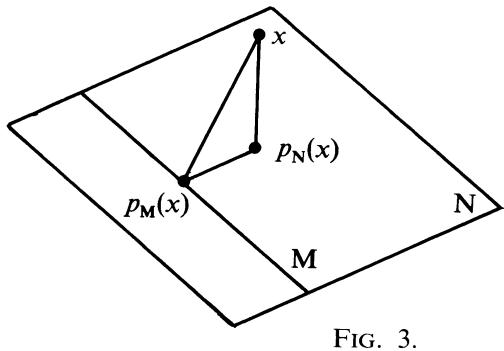
\includegraphics[keepaspectratio]{images/part002_dc4b20c6.jpg}}

\subsection{Dual of a hilbertian space}

THEOREM 3. --- Let E be a hilbertian space. For every \(x \in E\) , let \(x^{*}\) be the continuous linear form \(y \mapsto \langle x | y \rangle\) on E; the mapping \(x \mapsto x^{*}\) is a bijective, semi-linear (for the automorphism \(\xi \mapsto \overline{\xi}\) ) mapping from E onto its dual \(E'\) , and an isometry from the normed space E onto the normed space \(E'\) .

The mapping \(x \mapsto x^*\) is semi-linear by (2) (V, p.~1) and by virtue of the Cauchy-Schwarz inequality, we have \(\| x^* \| = \sup_{\| y \| \leqslant 1} |\langle x | y \rangle| = \| x \|\) , hence \(x \mapsto x^*\) is an isometry from E into E', and in particular, is injective. To complete the proof, we need to prove that for all \(x' \neq 0\) in E', there exists \(x \in E\) such that \(x' = x^*\) . But the hyperplane \(H = Ker x'\) is closed in E; its orthogonal is a line D. Let \(b\) be a non-zero element of D; the kernel of the linear form \(b^*\) is equal to H and hence there exists a scalar \(\lambda \neq 0\) such that \(x' = \lambda . b^* = (\overline{\lambda}. b)^*\) . Q.E.D.

The mapping \(x \mapsto x^{*}\) from E onto its dual \(E'\) is said to be canonical. The inverse mapping from \(E'\) onto E is also called canonical and is denoted by \(x' \mapsto x'^{*}\) . We have

\[
\langle x | y \rangle = \langle y, x ^ {*} \rangle , \quad \langle x, x ^ {\prime} \rangle = \langle x ^ {\prime *} | x \rangle\tag{17}
\]

for \(x, y\) in E and \(x'\) in E'. Also \((x^{*})^{*} = x\) for \(x \in \mathbf{E}\) .

When K is R, the mapping \(x \mapsto x^{*}\) is linear. We shall transfer the scalar product of E to \(E'\) by this mapping. When \(K = C\) , we can consider the mapping \(x \mapsto x^{*}\) as an isomorphism from the vector space \(\overline{E}\) , the conjugate of E onto \(E'\) (V, p.~6). We shall transfer the scalar product of \(\overline{E}\) to \(E'\) by this mapping.

In the two cases considered, \(E'\) is a hilbertian space and we have the formulae

\[
\langle x ^ {*} | y ^ {*} \rangle = \overline {{\langle x | y \rangle}}, \quad \langle x ^ {\prime} | x ^ {\prime} \rangle = \| x ^ {\prime} \| ^ {2}
\]

for \(x, y\) in \(\mathbf{E}\) and \(x'\) in \(\mathbf{E}'\) .

To say that the vector \(x \in E\) is orthogonal to a vector \(y \in E\) is equivalent to saying that the linear form \(x^{*} \in E'\) is orthogonal to y in the sense defined in II, p.~41 (this justifies the use of the word « orthogonal » in the two cases). If M is a closed vector subspace of E, the subspace \(M^{\circ}\) orthogonal to M in \(E'\) (II, p.~44) is the image under \(x \mapsto x^{*}\) of the orthogonal of M in E, defined in V, p.~13 (this justifies the use of the notation \(M^{\circ}\) in the two cases).

COROLLARY 1.--- In order that the family \((x_{i})_{i\in I}\) of points of a hilbertian space E be total, it is necessary and sufficient that the relations \(\langle x_{i}|y\rangle = 0\) for \(y \in E\) and for all indices \(i \in I\) imply that y = 0.

In fact, this says that 0 is the only vector of \(\mathbf{E}'\) which is orthogonal to all the \(x_{i}\) (II, p.~43 and IV, p.~1).

COROLLARY 2. --- Let E and F be two hilbertian spaces. For \(u \in \mathcal{L}(\mathrm{E};\mathrm{F})\) , \(x \in \mathrm{E}\) and \(y \in \mathrm{F}\) , put

\[
\Phi_ {u} (y, x) = \langle y | u (x) \rangle .\tag{18}
\]

The mapping \(u \mapsto \Phi_u\) is an isomorphism from the Banach space \(\mathcal{L}(\mathrm{E};\mathrm{F})\) onto the space of all continuous sesquilinear \(^1\) forms on \(\mathrm{F} \times \mathrm{E}\) , endowed with the norm

\[
\| f\| = \sup_{\substack{x\in \mathbf{E},  y\in \mathbf{F}\\ \| x\| \leqslant 1, \| y\| \leqslant 1}}\left|f(y,x)\right|.\tag{19}
\]

It is clear that \(\Phi_u\) is sesquilinear and continuous for all \(u \in \mathcal{L}(\mathrm{E};\mathrm{F})\) . Conversely, let \(f\) be a continuous sesquilinear form on \(\mathrm{F} \times \mathrm{E}\) . For every \(x \in \mathrm{E}\) , the mapping \(y \mapsto \overline{f(y,x)}\) is a continuous linear form on the hilbertian space \(\mathrm{F}\) . By th. 3, for every \(x \in \mathrm{E}\) , there exists a unique element \(u(x)\) in \(\mathrm{F}\) such that \(\overline{f(y,x)} = \langle u(x)|y\rangle\) for all \(y \in \mathrm{F}\) . The mapping \(u: x \mapsto u(x)\) from \(\mathrm{E}\) into \(\mathrm{F}\) is linear and we have

\[
\begin{array}{l} \| f \| = \sup _ {\| x \| \leqslant 1} \sup _ {\| y \| \leqslant 1} | f (y, x) | = \sup _ {\| x \| \leqslant 1} \sup _ {\| y \| \leqslant 1} | \langle y | u (x) \rangle | \\ = \sup _ {\| x \| \leqslant 1} \| u (x) \|; \end{array}
\]

hence \(u\) belongs to \(\mathcal{L}(\mathrm{E};\mathrm{F})\) , \(f = \Phi_u\) and \(\| u\| = \| f\|\) . This proves cor. 2.

\(^{1}\) Recall (A, IX, § 1, No.~5) that a sesquilinear form (on the left) f on F × E is a mapping from F × E into K which satisfies relations (1) and (2) of V, p.~1.

The canonical mapping from E into its bidual \(E''\) (IV, p.~14) maps E onto \(E''\) , in other words (IV, p.~16), E is a reflexive Banach space. In fact, if E is a real (resp. complex) hilbertian space, the canonical mapping \(\phi\) from \(E'\) onto E is an isomorphism from the normed space \(E'\) onto E (resp. onto the conjugate space \(\overline{E}\) of E); applying th. 3 to E (resp. \(\overline{E}\) ), we see that every continuous linear form on the normed space \(E'\) is of the form \(x' \mapsto \langle \phi(x') | x \rangle = \langle x, x' \rangle\) with \(x \in E\) , hence our assertion follows.

As a consequence (IV, p.~17, prop. 6):

THEOREM 4. --- In a hilbertian space E, the unit ball is weakly compact.

PROPOSITION 10. --- If, in a hilbertian space E, a filter F converges weakly to \(x_{0}\) , and if moreover \(\lim_{\mathfrak{F}} \|x\| = \|x_{0}\|\) , then F converges to \(x_{0}\) for the initial topology of E. In fact, \(\|x - x_{0}\|^{2} = \|x\|^{2} - 2R \langle x|x_{0} \rangle + \|x_{0}\|^{2}\) . Since \(\langle x|x_{0}\rangle\) tends to \(\|x_{0}\|^{2}\) with respect to F by hypothesis, and \(\|x\|\) tends to \(\|x_{0}\|\) with respect to F, \(\|x - x_{0}\|\) tends to 0 with respect to F, hence the proposition.

Remark. --- If E is a Hausdorff prehilbertian space and \(\hat{E}\) the hilbertian space completion of E, we know (III, p.~16) that the dual \(E'\) of E can be identified with the dual of \(\hat{E}\) ; it then follows from th. 3 (V, p.~15) that every continuous linear form on E can be written in a unique way as \(x \mapsto \langle a|x\rangle\) , where \(a \in \hat{E}\) .

\section{ORTHOGONAL FAMILIES IN A HILBERTIAN SPACE}

\subsection{External hilbertian sum of hilbertian spaces}

PROPOSITION 1. --- Let \((\mathrm{E}_i)_{i\in \mathbf{I}}\) be a family of hilbertian spaces, \(\mathbf{P}\) the product vector space \(\prod_{i\in \mathbf{I}}\mathrm{E}_i\) and \(\mathbf{E}\) the subset of \(\mathbf{P}\) consisting of all families \(\mathbf{x} = (x_i)_{i\in \mathbf{I}}\) such that \(\sum_{i\in \mathbf{I}}\| x_i\|^2\) is finite.

\begin{enumerate}
\def\labelenumi{\alph{enumi})}
\item
  E is a vector subspace of \(\mathbf{P}\) .
\item
  For every \(\mathbf{x} = (x_i)_{i\in \mathbf{I}}\) and \(\mathbf{y} = (y_i)_{i\in \mathbf{I}}\) in E, the family \((\langle x_i|y_i\rangle)_{i\in \mathbf{I}}\) is summable. If we put \(\langle \mathbf{x}|\mathbf{y}\rangle = \sum_{i\in \mathbf{I}}\langle x_i|y_i\rangle\) , we define a positive separating hermitian form on E.
\item
  For the scalar product so defined, \(\mathbf{E}\) is a hilbertian space; the direct sum \(\mathbf{S}\) of the \(\mathbf{E}_i\) is dense in \(\mathbf{E}\) .
\end{enumerate}

For \(\mathbf{x} = (x_{i})_{i\in \mathbf{I}}\) and \(\mathbf{y} = (y_i)_{i\in \mathbf{I}}\) in E, we have

\[
\left\| x _ {i} + y _ {i} \right\| ^ {2} \leqslant 2 \left(\left\| x _ {i} \right\| ^ {2} + \left\| y _ {i} \right\| ^ {2}\right),
\]

hence \(\mathbf{x} + \mathbf{y} = (x_i + y_i)_{i\in I}\) belongs to E. This proves \(a)\) .

By the Cauchy-Schwarz inequality, we have

\[
\left| \left\langle x _ {i} \mid y _ {i} \right\rangle \right| \leqslant \| x _ {i} \| \cdot \| y _ {i} \| \leqslant \frac {1}{2} \left(\left\| x _ {i} \right\| ^ {2} + \left\| y _ {i} \right\| ^ {2}\right)
\]

hence \(\sum_{i\in \mathbf{I}}|\langle x_i|y_i\rangle | < +\infty\) . If \(x\neq 0\) , we have \(\langle \mathbf{x}|\mathbf{x}\rangle = \sum_{i\in \mathbf{I}}\| x_i\|^2 >0\) , hence assertion \(b)\) follows.

We recall that S is the subspace of P consisting of all families \(\mathbf{x} = (x_{i})_{i \in \mathbf{I}}\) such that the set of all \(i \in I\) for which \(x_{i} \neq 0\) is finite. It follows immediately that S is dense in E; hence it remains to prove that E is complete for the topology \(T_{1}\) obtained by the norm \(\|x\| = \langle x|x\rangle^{1/2}\) . Let \(T_{2}\) be the topology induced on E by the product topology on \(\prod_{i \in I} E_{i}\) . For every r \textgreater{} 0, let \(B_{r}\) be the set of all \(x \in E\) such that \(\|x\| \leqslant r\) . This relation implies that we have \(\sum_{i \in J} \|x_{i}\|^{2} \leqslant r^{2}\) for every finite subset J of I, and so \(B_{r}\) is a closed subset of \(\prod_{i \in I} E_{i}\) , hence also complete. The fact that E is complete for \(T_{1}\) now follows from GT, III, §3, No.~5, cor. 2 to prop. 10.

DEFINITION 1. --- Let \((\mathrm{E}_{i})_{i\in\mathrm{I}}\) be a family of hilbertian spaces. The hilbertian space E defined in prop. 1 is called the external hilbertian sum of the family \((\mathrm{E}_{i})_{i\in\mathrm{I}}\) and written as \(\bigoplus_{i\in I} E_{i}\) or \(\bigoplus_{i\in I} E_{i}^{1}\) .

\(^{1}\) Care must be taken not to confuse this notation with that of the « algebraic » direct sum of the spaces \(E_{i}\) (A, II, § 1, No.~6).

Let \(f_{i}\) be the mapping from \(E_{i}\) into \(E\) which transforms \(z \in E_{i}\) into an element \((x_{k}) \in E\) such that \(x_{k} = 0\) for all \(k \neq i\) and \(x_{i} = z\) ; it is clear that \(f_{i}\) is an isomorphism from the hilbertian space \(E_{i}\) onto a closed vector subspace of \(E\) . We say that \(f_{i}\) is the canonical mapping from \(E_{i}\) into \(E\) and we shall generally identify \(E_{i}\) with its image in \(E\) by this isomorphism. With this convention, \(E_{i}\) and \(E_{k}\) are orthogonal in \(E\) for \(i \neq k\) , and \(E\) is the closed vector subspace generated by the union of the subspaces \(E_{i}\) .

When I is finite, E is the direct sum of the \(E_{i}\) ; since the canonical projector from E onto \(E_{i}\) is continuous for all \(i \in I\) , E is also the topological direct sum of the \(E_{i}\) (GT, III, § 6, No.~2, prop. 2). If \(I = \left(1, n\right)\) , we also write \(E_{1} \oplus E_{2} \oplus \ldots \oplus E_{n}\) instead of \(\bigoplus_{i=1}^{n} E_{i}\) .

Example. --- Let E be a hilbertian space and I a set of indices. Let \(\ell_{\mathrm{E}}^{2}(\mathrm{I})\) denote the external hilbertian sum of the family \((\mathrm{E}_{i})_{i\in\mathrm{I}}\) where \(E_{i}=E\) for all \(i\in I\) . In other words, \(\ell_{\mathrm{E}}^{2}(\mathrm{I})\) is the space of all families \(\mathbf{x}=(x_{i})_{i\in\mathrm{I}}\) of elements of E such that \(\sum_{i\in I}\|x_{i}\|^{2}<+\infty\) , endowed with the scalar product \(\langle x|y\rangle=\sum_{i\in I}\langle x_{i}|y_{i}\rangle\) (space of square summable families of elements of E indexed by I). We put \(\ell^{2}(\mathrm{I})=\ell_{\mathrm{K}}^{2}(\mathrm{I})\) .

\subsection{Hilbertian sum of orthogonal subspaces of a hilbertian space}

DEFINITION 2. --- A hilbertian space E is said to be a hilbertian sum of a family \((\mathbf{E}_{i})_{i\in I}\) of closed vector subspaces of E when :

\begin{enumerate}
\def\labelenumi{\arabic{enumi})}
\item
  for two distinct indices \(i\) , \(k\) in I, the subspaces \(\mathrm{E}_i\) and \(\mathrm{E}_k\) are orthogonal in E;
\item
  the closed vector subspace generated by the union of the \(\mathbf{E}_i\) is E.
\end{enumerate}

THEOREM 1. --- Let E be a hilbertian space which is a hilbertian sum of a family \((\mathrm{E}_{i})_{i\in\mathbf{I}}\) of closed vector subspaces of E. There exists an isomorphism f and only one, from E onto the external hilbertian sum \(\bigoplus_{i\in I}E_{i}=F\) of the family \((\mathrm{E}_{i})\) such that, for all \(i\in I\) , the restriction of \(f\) to \(\mathbf{E}\) is the canonical mapping \(f_{i}\) from \(\mathbf{E}_i\) into \(\mathbf{F}\) .

Let \(S \subset F\) be the « algebraic » direct sum of the \(E_i\) , and let \(g\) be the linear mapping \((x_i)_{i \in I} \mapsto \sum_{i \in I} x_i\) from \(S\) into \(E\) . We shall show that \(g\) is an isomorphism from the prehilbertian space S onto the (prehilbertian) subspace \(g(S)\) of E, generated by the union of the \(E_{i}\) : for, for two elements \(\mathbf{x} = (x_{i})_{i \in \mathrm{I}}\) , \(\mathbf{y} = (y_{i})_{i \in \mathrm{I}}\) , we have

\[
\langle g (\mathbf {x}) | g (\mathbf {y}) \rangle = \left\langle \sum_ {i \in \mathrm{I}} x _ {i} \right| \sum_ {i \in \mathrm{I}} y _ {i} \rangle = \sum_ {(i, k) \in \mathrm{I} \times \mathrm{I}} \left\langle x _ {i} \mid y _ {k} \right\rangle .
\]

But if \(i \neq k\) , \(\langle x_i | y_k \rangle = 0\) by hypothesis, hence

\[
\langle g (\mathbf {x}) | g (\mathbf {y}) \rangle = \sum_ {i \in \mathbf {I}} \langle x _ {i} | y _ {i} \rangle = \langle \mathbf {x} | \mathbf {y} \rangle ;
\]

this proves our assertion. Since S is dense in F and \(g(S)\) dense in E, the isomorphism g extends to an isomorphism \(\overline{g}\) from F onto E (V, p.~8, cor.). It is clear that the inverse isomorphism f of \(\overline{g}\) is the required mapping; its uniqueness follows from the fact that the closed subspace of E generated by the union of the \(E_{i}\) is E itself.

When E is the hilbertian sum of a family \((\mathrm{E}_{i})_{i\in I}\) of subspaces, we shall often identify E with the external hilbertian sum F of the \(E_{i}\) by means of the isomorphism f.~If the set I is finite, saying that E is the hilbertian sum of the family \((\mathrm{E}_{i})_{i\in I}\) means that the \(E_{i}\) are two by two orthogonal and that the vector space E is the direct sum of the family \((\mathrm{E}_{i})_{i\in I}\) of subspaces.

COROLLARY 1. --- Let E be a hilbertian space, which is a hilbertian sum of a family \((\mathbf{E}_{i})_{i\in\mathbf{I}}\) of closed vector subspaces of E; for all \(i\in I\) , let \(p_{E_{i}}\) be the orthoprojector (V, p.~13) from E onto \(E_{i}\) .

\begin{enumerate}
\def\labelenumi{\alph{enumi})}
\tightlist
\item
  For all \(x \in \mathbb{E}\) , the family \((\| p_{\mathbf{E}_i}(x)\|^{2})_{i\in \mathbf{I}}\) is summable in \(\mathbf{R}\) , the family \((p_{\mathbf{E}_i}(x))_{i\in \mathbf{I}}\) is summable in \(\mathbb{E}\) , and we have
\end{enumerate}

\[
\left\| x \right\| ^ {2} = \sum_ {i \in \mathbf {I}} \left\| p _ {\mathrm{E} _ {i}} (x) \right\| ^ {2}, \quad x = \sum_ {i \in \mathbf {I}} p _ {\mathrm{E} _ {i}} (x).
\]

\begin{enumerate}
\def\labelenumi{\alph{enumi})}
\setcounter{enumi}{1}
\item
  Conversely, if \((x_{i})_{i\in \mathbf{I}}\) is a family of elements of \(\mathbf{E}\) such that \(x_{i}\in E_{i}\) for all \(i\in \mathbf{I}\) and \(\sum_{i\in \mathbf{I}}\| x_i\|^2 < + \infty\) , this family is summable, and the sum \(x\) is the only point of \(\mathbf{E}\) for which \(p_{\mathrm{E}_i}(x) = x_i\) for all \(i\in \mathbf{I}\) .
\item
  For every pair of points \(x, y\) of \(\mathbf{E}\) , we have
\end{enumerate}

\[
\langle x | y \rangle = \sum_ {i \in \mathbf {I}} \left\langle p _ {\mathrm{E} _ {i}} (x) \mid p _ {\mathrm{E} _ {i}} (y) \right\rangle .
\]

These properties are in fact obvious for the external hilbertian sum of the \(\mathbf{E}_i\) , and can be transferred to \(\mathbf{E}\) by isomorphism.

COROLLARY 2. --- Let E be a Hausdorff prehilbertian space, \((\mathrm{E}_{i})_{i\in\mathrm{I}}\) a family of complete vector subspaces of E such that, for every pair of distinct indices i, k in I, the subspaces \(E_{i}\) and \(E_{k}\) are orthogonal. Let V be the closed vector subspace of E generated by the union of the \(E_{i}\) . For every \(i\in I\) , let \(p_{E_{i}}\) be the orthoprojector from E onto \(E_{i}\) . Let \(x\in E\) .

\begin{enumerate}
\def\labelenumi{\arabic{enumi})}
\item
  We have \(\sum\left\|p_{E_{i}}(x)\right\|^{2}\leqslant\left\|x\right\|^{2}\) .
\item
  The following conditions are equivalent: a) \(x \in \mathbf{V}\) ; b) \(\sum_{i \in I} \| p_{\mathrm{E}_i}(x) \|^2 = \| x \|^2\) ; c) the family \((p_{\mathrm{E}_i}(x))_{i \in I}\) is summable in E, and we have \(x = \sum_{i \in I} p_{\mathrm{E}_i}(x)\) .
\item
  Suppose V is complete. Then the family \((p_{\mathrm{E}_i}(x))_{i\in \mathbf{I}}\) is summable in E, and
\end{enumerate}

\[
p _ {\mathbf {V}} (x) = \sum_ {i \in \mathbf {I}} p _ {\mathrm{E} _ {i}} (x), \quad \left\| p _ {\mathbf {V}} (x) \right\| ^ {2} = \sum_ {i \in \mathbf {I}} \left\| p _ {\mathrm{E} _ {i}} (x) \right\| ^ {2},
\]

where \(p_{V}\) denotes the orthoprojector from E onto V.

Let \(\hat{\mathbf{E}}\) be the hilbertian space completion of \(\mathbf{E}\) ; we identify \(\mathbf{E}\) with a dense subspace of \(\hat{\mathbf{E}}\) ; the \(\mathbf{E}_i\) , being complete, are closed subspaces of \(\hat{\mathbf{E}}\) . The closure \(\overline{\mathbf{V}}\) of \(\mathbf{V}\) in \(\hat{\mathbf{E}}\) is the closed vector subspace of \(\hat{\mathbf{E}}\) generated by the union of the \(\mathbf{E}_i\) , and \(\mathbf{V} = \overline{\mathbf{V}} \cap \mathbf{E}\) . The space \(\hat{\mathbf{E}}\) is the hilbertian sum of the \(\mathbf{E}_i\) and of the subspace \(\mathbf{W}\) , the orthogonal complement of \(\overline{\mathbf{V}}\) in \(\hat{\mathbf{E}}\) ; put \(x_0 = p_{\mathrm{W}}(x)\) and \(x_i = p_{\mathrm{E}_i}(x)\) for all \(i \in \mathbf{I}\) . By cor. 1, we have \(\| x\|^2 = \| x_0\|^2 + \sum_{i \in \mathbf{I}} \| x_i\|^2\) , and \(x = x_0 + \sum_{i \in \mathbf{I}} x_i\) in \(\hat{\mathbf{E}}\) . This implies assertion 1), and the fact that conditions \(b)\) and \(c)\) of 2) are equivalent to the condition \(x_0 = 0\) , hence to the condition \(x \in \mathbf{V}\) . Finally, if \(\mathbf{V}\) is complete, and if we put \(x' = p_{\mathrm{V}}(x)\) , we have \(x' - x_i = (x - x_i) - (x - p_{\mathrm{V}}(x))\) , hence \(x' - x_i\) is orthogonal to \(\mathbf{E}_i\) , and so \(x_i = p_{\mathrm{E}_i}(x')\) for all \(i \in \mathbf{I}\) ; it is now enough to apply property 2) to the vector \(x'\) .

Remark. --- Let E be a Hausdorff prehilbertian space, \((\mathrm{V}_{i})_{i\in\mathrm{I}}\) a family of vector subspaces of E such that for every pair of distinct indices i, k, the subspaces \(V_{i}\) and \(V_{k}\) are orthogonal. Then, for every \(k\in I\) , the intersection of \(V_{k}\) and of the closed vector subspace \(W_{k}\) generated by the union of the \(V_{i}\) for all \(i\neq k\) reduces to 0 for, if x belongs to \(V_{k}\) and also to \(W_{k}\) , then it is orthogonal to all the \(V_{i}\) for \(i\neq k\) , hence to \(W_{k}\) . In particular, x is orthogonal to itself, hence is zero.

PROPOSITION 2. --- Let E be a hilbertian space and \((\mathrm{V}_{\lambda})_{\lambda\in\mathrm{L}}\) a family of closed vector subspaces of E; for every \(\lambda\in L\) , let \((\mathrm{W}_{\lambda\mu})_{\mu\in\mathrm{M}_{\lambda}}\) be a family of closed vector subspaces of \(V_{\lambda}\) such that \(V_{\lambda}\) is the closed vector subspace generated by the union of this family. In order that E is the hilbertian sum of the family \((\mathrm{W}_{\lambda\mu})_{\lambda\in\mathrm{L},\mu\in\mathrm{M}_{\lambda}}\) , it is necessary and sufficient that E is the hilbertian sum of the family \((\mathrm{V}_{\lambda})_{\lambda\in\mathrm{L}}\) and that, for each \(\lambda\in L\) , \(V_{\lambda}\) is the hilbertian sum of the family \((\mathrm{W}_{\lambda\mu})_{\mu\in\mathrm{M}_{\lambda}}\) (« associativity of the hilbertian sum »). To show that the condition is necessary, it is enough to see that \(V_{\alpha}\) and \(V_{\beta}\) are orthogonal if \(\alpha\neq\beta\) . But, every element of \(W_{\alpha\mu}\) ( \(\mu\in M_{\alpha}\) ) is orthogonal to all the \(W_{\beta\nu}\) ( \(\nu\in M_{\beta}\) ), hence to the closed vector subspace \(V_{\beta}\) which they generate; the same argument then shows that every element of \(V_{\beta}\) is orthogonal to \(V_{\alpha}\) , being orthogonal to all the \(W_{\alpha\mu}\) ( \(\mu\in M_{\alpha}\) ).

To show that the condition is sufficient, it is enough to verify that, if it is satisfied, \(\mathrm{E}\) is equal to the closed vector subspace \(\mathrm{F}\) generated by the union of the \(\mathbf{W}_{\lambda \mu}\) (\(\lambda \in \mathbf{L}\), \(\mu\in M_{\lambda}\)); but, for each \(\lambda\in L\) , F contains the closed vector subspace generated by the union of the \(W_{\lambda\mu}\) such that \(\mu\in M_{\lambda}\) , that is, F contains \(V_{\lambda}\) ; hence F is the closed vector subspace generated by the union of the \(V_{\lambda}\) , which is E by hypothesis.

\subsection{Orthonormal families}

DEFINITION 3. --- In a prehilbertian space, a family \((e_{i})_{i\in\mathbf{I}}\) of vectors is said to be orthogonal if \(e_{i}\) and \(e_{k}\) are orthogonals for all \(i\neq k\) , and is said to be orthonormal, if in addition \(\|e_{i}\|=1\) for all \(i\in I\) .

A subset S of E such that the family defined by the identity mapping from S onto itself is orthonormal is said to be an orthonormal set. If \((e_{i})_{i\in I}\) is an orthonormal family, the mapping \(i\mapsto e_{i}\) is injective; we can then talk indifferently of an orthonormal family or an orthonormal set.

If \((e_i)_{i\in I}\) is an orthonormal family, the complete one dimensional vector subspaces \(\mathbf{D}_i = \mathbf{K}e_i\) are two by two orthogonal. For every \(x\in E\) , the orthogonal projection of \(x\) on \(\mathbf{D}_i\) is \(\lambda_i e_i\) with \(\langle e_i|x - \lambda_i e_i\rangle = 0\) , which gives \(\langle e_i|x\rangle = \lambda_i\langle e_i|e_i\rangle = \lambda_i\) . The results of No.~2 applied to the subspaces \(\mathbf{D}_i\) imply the following propositions:

PROPOSITION 3. --- In a Hausdorff prehilbertian space E, every orthonormal family is topologically independent.

We note that this property immediately follows from the characterization of topologically independent families (IV, p.~1 and II, p.~43, cor. 2), on account of the identification of the dual of E with the completion of E or with the space conjugate to E according as K is equal to R or C (V, p.~17, Remark).

PROPOSITION 4. --- Let E be a Hausdorff prehilbertian space, \((e_{i})_{i\in I}\) an orthonormal family in E, V the closed vector subspace of E generated by the \(e_{i}\) .

\begin{enumerate}
\def\labelenumi{\arabic{enumi})}
\tightlist
\item
  For every \(x \in E\) , we have
\end{enumerate}

\[
\sum_ {i \in \mathbf {I}} \left| \langle e _ {i} | x \rangle \right| ^ {2} \leqslant \| x \| ^ {2}\tag{1}
\]

(Bessel's inequality); here the set of all \(i \in \mathbf{I}\) such that \(\langle e_i|x\rangle \neq 0\) is countable. Moreover, the following conditions are equivalent: a) \(x \in \mathbf{V}\) ; b) \(\|x\|^2 = \sum_{i \in \mathbf{I}} |\langle e_i|x\rangle|^2\) ; c) the family \(\langle e_i|x\rangle\) . \(e_i\) is summable in E, and \(x = \sum_{i \in \mathbf{I}} \langle e_i|x\rangle\) . \(e_i\) .

\begin{enumerate}
\def\labelenumi{\arabic{enumi})}
\setcounter{enumi}{1}
\item
  If \(\mathbf{V}\) is complete, then the family of all \(\langle e_i|x\rangle\) . \(e_i\) is summable in \(\mathbf{E}\) for all \(x\in\mathbf{E}\) , and \(\sum_{i\in\mathbf{I}}\langle e_i|x\rangle\) . \(e_i=p_{\mathbf{V}}(x)\) , \(\sum_{i\in\mathbf{I}}|\langle e_i|x\rangle|^2=\|p_{\mathbf{V}}(x)\|^2\) .
\item
  Suppose V is complete. For every family \((\lambda_{i})_{i\in\mathbf{I}}\) of scalars such that \(\sum_{i\in I}|\lambda_{i}|^{2}<+\infty\) , there exists a unique point \(x\in V\) such that \(\langle e_{i}|x\rangle=\lambda_{i}\) for all \(i\in I\) . If \((\mu_{i})_{i\in I}\) is a second family of scalars such that \(\sum_{i\in I}\left|\mu_{i}\right|^{2}<+\infty\) , and if \(y\in V\) is such that \(\langle e_{i}|y\rangle=\mu_{i}\) for all \(i\in I\) , then \(\langle x|y\rangle=\sum_{i\in I}\overline{\lambda}_{i}\mu_{i}\) .
\end{enumerate}

PROPOSITION 5. --- Let \((e_i)_{i \in I}\) be an orthonormal family in a Hausdorff prehilbertian space E. The following properties are equivalent :

\begin{enumerate}
\def\labelenumi{\alph{enumi})}
\item
  the family \((e_i)\) is total;
\item
  for every \(x \in E\) , the family \(\langle e_{i}|x\rangle\) . \(e_{i}\) is summable in E, and we have \(x = \sum_{i \in I} \langle e_{i}|x\rangle\) . \(e_{i}\) ;
\item
  for every \(x \in E\) ,
\end{enumerate}

\[
\left\| x \right\| ^ {2} = \sum_ {i \in \mathbf {I}} \left| \langle e _ {i} | x \rangle \right| ^ {2}\tag{2}
\]

(Parseval's relation).

When E is hilbertian these conditions are also equivalent to :

\begin{enumerate}
\def\labelenumi{\alph{enumi})}
\setcounter{enumi}{3}
\tightlist
\item
  the relations \(\langle e_i|x\rangle = 0\) for all \(i\in \mathrm{I}\) imply that \(x = 0\) .
\end{enumerate}

The equivalence of conditions a), b), c) follows immediately from prop. 4. When E is hilbertian, the equivalence of conditions a) and d) follows from cor. 1 of V, p.~16.

DEFINITION 4. --- An orthonormal and total family in a Hausdorff prehilbertian space E is called an orthonormal basis of E.

An orthonormal basis of a Hausdorff prehilbertian space E is also an orthonormal basis of the completion of E.

Let \((e_{i})_{i\in I}\) be an orthonormal basis of E; for every \(x\in E\) , the numbers \(\langle e_{i}|x\rangle\) are called, by abuse of language, the coordinates of x with respect to the basis \((e_{i})\) . For every x and y in E, we have

\[
\langle x | y \rangle = \sum_ {i \in \mathbf {I}} \overline {{\langle e _ {i} | x \rangle}} \langle e _ {i} | y \rangle .\tag{3}
\]

An orthonormal basis of E is not, in general, a basis of E over the field K in the sense defined in A, II, p.~25; to avoid any confusion we shall always say that a basis of a prehilbertian space E in the sense of loc. cit. is an algebraic basis of E over K.

Let E and F be two Hausdorff prehilbertian spaces and u a continuous linear mapping from E into F. Let \((e_{i})_{i\in I}\) (resp. \((f_{j})_{j\in J}\) ) be an orthonormal basis of E (resp. F). Put

\[
u _ {j i} = \langle f _ {j} | u (e _ {i}) \rangle
\]

for \(i \in \mathbf{I}\) , \(j \in \mathbf{J}\) . The family \((u_{ji})_{(i,j) \in \mathbf{I} \times \mathbf{J}}\) is called the matrix of \(u\) with respect to the ortho-normal bases \((e_i)\) and \((f_j)\) . Let \(x \in \mathbf{E}\) and \(y = u(x)\) ; if we write \(\xi_i = \langle e_i | x \rangle\) and \(\eta_j = \langle f_j | y \rangle\) for the coordinates of \(x\) and \(y\) respectively, we get \(\eta_j = \sum_{i \in \mathbf{I}} u_{ji} \xi_i\) for all \(j \in \mathbf{J}\) . When \((e_i)\) is an algebraic basis of \(E\) and \((f_j)\) an algebraic basis of \(F\) , our definition is consistent with that of A, II, § 10, No.~4.

Example. --- Let E be the space of all complex valued continuous functions on R, such that \(f(x + n) = f(x)\) for \(x \in R\) and \(n \in Z\) . We assign to E the scalar product defined by

\[
\langle f | g \rangle = \int_ {0} ^ {1} \overline {{{{f (t)}}}} g (t) d t.
\]

Then E is a Hausdorff prehilbertian space, but is not complete. For every integer \(n \in Z\) , let \(e_{n}(x) = \mathbf{e}(nx)\) . It is immediate that the family \((e_{n})_{n \in \mathbf{Z}}\) is orthonormal in E. Moreover, the topology of uniform convergence on E is finer than the topology deduced from the norm \(\|f\|_{2} = \langle f | f \rangle^{1/2}\) . The family \((e_{n})_{n \in \mathbf{Z}}\) is total in E for the uniform convergence (GT, X, § 4, No.~4), and a fortiori in the prehilbertian space E. Hence \((e_{n})_{n \in \mathbf{Z}}\) is an orthonormal basis of E.

\subsection{Orthonormalisation}

THEOREM 2. --- For every orthonormal set L in a hilbertian space E, there exists an orthonormal basis B of E containing L.

In fact, let D be the family of all orthonormal subsets of E, linearly ordered by inclusion; it is immediate that this family has finite character (S, III, § 4, No.~5). Hence there exists a maximal family B in D containing L, by th. 1 of S, III, § 4, No.~5. It remains to prove that B is a total set. If not, there will exist a vector \(y \neq 0\) which is orthogonal to all the vectors of B (V, p.~22, prop. 5), and multiplying y by a suitable scalar, we can assume that \(\|y\| = 1\) ; then, \(B \cup \{y\}\) will be an orthonormal set distinct from B and containing B; this contradicts the definition of B; hence the theorem.

COROLLARY 1. --- In every hilbertian space, there exists an orthonormal basis.

It is enough to apply th. 2 to the case L = ∅.

COROLLARY 2. --- Every hilbertian space is isomorphic to a space \(\ell^2 (\mathbf{I})\) .

More precisely, let \((e_{i})_{i\in I}\) be an orthonormal basis of a hilbertian space E. By props. 4 (V, p.~21) and 5 (V, p.~22), the mapping \(\phi\) defined by

\[
\phi (x) = \big (\langle e _ {i} | x \rangle \big) _ {i \in \mathrm{I}}\tag{4}
\]

is a hilbertian space isomorphism from E onto \(\ell^2 (\mathrm{I})\) . The inverse isomorphism \(\psi\) is defined by

\[
\psi ((\lambda_ {i}) _ {i \in \mathbf {I}}) = \sum_ {i \in \mathbf {I}} \lambda_ {i} e _ {i}.\tag{5}
\]

PROPOSITION 6. --- Let E be a Hausdorff prehilbertian space, and let \((a_{n})_{n\in\mathbb{I}}\) (I an interval of N with origin 1) be a countable (finite or not) independent family of vectors of E. There exists an orthonormal family \((e_{n})_{n\in\mathbb{I}}\) , and only one, in E, with the following properties :

\begin{enumerate}
\def\labelenumi{\arabic{enumi})}
\item
  for every integer \(p \in \mathbf{I}\) , the vector subspace of \(\mathbf{E}\) generated by \(e_1, e_2, \ldots, e_p\) is identical with the vector subspace of \(\mathbf{E}\) generated by \(a_1, a_2, \ldots, a_p\) ;
\item
  for every integer \(p \in \mathbf{I}\) , the number \(\langle a_p | e_p \rangle\) is real and \(> 0\) .
\end{enumerate}

In fact, let \(V_{n}\) be the subspace (of dimension n) generated by \(a_{1}, a_{2}, ..., a_{n}\) . If \(n + 1 \in I\) and \(b_{n+1} = a_{n+1} - p_{\mathrm{V}_{n}}(a_{n+1})\) (where \(p_{V_{n}}\) is the orthoprojector onto the complete subspace \(V_{n}\) ), the line \(Kb_{n+1}\) is the orthogonal of \(V_{n}\) in \(V_{n+1}\) . If the \(e_{n}\) satisfy condition 1) of the proposition, we must have \(e_{n+1} = \lambda b_{n+1}\) ; the condition \(\|e_{n+1}\| = 1\) then implies \(|\lambda|^2 \|b_{n+1}\|^2 = 1\) and the condition \(\langle a_{n+1}|e_{n+1} \rangle > 0\) implies \(\lambda \langle a_{n+1}|b_{n+1} \rangle > 0\) ; this completely determines \(\lambda\) , and we have proved that we can determine, by induction, an orthonormal family \((e_n)_{n\in I}\) , and only one, so as to satisfy conditions 1) and 2) of the proposition.

The sequence \((e_{n})_{n\in\mathbb{I}}\) is said to be obtained by orthonormalisation from the independent family \((a_{n})_{n\in\mathbb{I}}\) . It is clear that the vector subspace generated by the family \((e_{n})\) is identical with the vector subspace generated by the family \((a_{n})\) . In particular, if \((a_{n})\) is a total sequence, so is \((e_{n})\) , which is then an orthonormal basis of E; hence we get:

COROLLARY. --- In every Hausdorff prehilbertian space E satisfying the first axiom of countability, there exists a countable orthonormal basis.

If E satisfies the first axiom of countability, then there exists a total sequence in E, and we can always extract an independent total family from such a sequence (A, II, § 7, No.~1, th. 2).

We can give examples of Hausdorff prehilbertian spaces not having any orthonormal basis (V, p.~70, exerc. 2).

Example. --- Let I be the interval \((-1,1)\) of R and E the vector space of real valued continuous functions on I. Let x denote the canonical injection from I into R, considered as an element of E. By the Stone-Weierstrass theorem the sequence \((x^{n})_{n\in\mathbf{N}}\) is total in E for the topology of uniform convergence GT, X, § 4, No.~2).

Consider E as a real Hausdorff prehilbertian space in which the scalar product is given by

\[
\langle f | g \rangle = \int_ {- 1} ^ {1} f (t) g (t) d t.
\]

The sequence \((x^{n})_{n\in \mathbb{N}}\) is then total in the prehilbertian space E. Let \((\Pi_n)_{n\in \mathbb{N}}\) be the sequence obtained by the orthonormalisation of the sequence \((x^n)_{n\in \mathbb{N}}\) . We can show that \(\Pi_n = (n + \frac{1}{2})^{1 / 2}\mathbf{P}_n\) , where the Legendre polynomial \(\mathbf{P}_n\) is defined by

\[
\mathrm{P} _ {n} (x) = \frac {1}{2 ^ {n} n !} \left(\frac {d}{d x}\right) ^ {n} (x ^ {2} - 1) ^ {n}.
\]

PROPOSITION 7. --- In a hilbertian space E, two orthonormal bases are equipotent.

Let B and C be two orthonormal bases of E. The case when one of the two sets B, C is finite is trivial, since a finite orthonormal basis is an algebraic basis of the space. Suppose therefore that B and C are infinite. For every \(x \in B\) , let \(C_{x}\) be the subset of C consisting of all \(y \in C\) such that \(\langle x | y \rangle \neq 0\) . The set \(C_{x}\) is countable (V, p.~21, prop. 4). For every \(y \in C\) , there exists \(x \in B\) such that \(y \in C_{x}\) , since B is an orthonormal basis and \(y \neq 0\) ; in other words C is the union of the countable sets \(C_{x}\) as x ranges over B. The cardinality of C is hence less than that of N × B, hence less than that of B (S, III, §6, No.~3, cor. 4); similarly, the cardinality of B is less than that of C; this completes the proof.

The cardinality of an arbitrary orthonormal basis of a hilbertian space E is called the hilbertian dimension of E.

COROLLARY 1. --- Given two orthonormal bases in a hilbertian space E, there exists an automorphism of E transforming the first basis into the second.

COROLLARY 2. --- In order that the hilbertian spaces \(\ell^2 (\mathbf{I})\) and \(\ell^2 (\mathbf{J})\) be isomorphic, it is necessary and sufficient that I and J are equipotent.

\section{TENSOR PRODUCT OF HILBERTIAN SPACES}

\subsection{Tensor product of prehilbertian spaces}

Let \(E_{1}\) and \(E_{2}\) be two prehilbertian spaces and let \(F = E_{1} \otimes E_{2}\) be the tensor product of the vector spaces \(E_{1}\) and \(E_{2}\) . Let \(x_{1} \in E_{1}\) and \(x_{2} \in E_{2}\) ; since the mapping \((y_{1}, y_{2}) \mapsto \langle x_{1}|y_{1} \rangle \langle x_{2}|y_{2} \rangle\) from \(E_{1} \times E_{2}\) into K is bilinear, there exists a linear form \(\phi_{x_{1},x_{2}}\) on \(E_{1} \otimes E_{2}\) such that

\[
\phi_ {x _ {1}, x _ {2}} (y _ {1} \otimes y _ {2}) = \langle x _ {1} | y _ {1} \rangle \langle x _ {2} | y _ {2} \rangle\tag{1}
\]

for \(y_{1} \in \mathrm{E}_{1}\) and \(y_{2} \in \mathrm{E}_{2}\) . Let \(z \in \mathrm{F}\) . The mapping \((x_{1}, x_{2}) \mapsto \overline{\phi_{x_{1},x_{2}}(z)}\) from \(\mathrm{E}_1 \times \mathrm{E}_2\) into \(\mathbf{K}\) is bilinear; this can be seen by writing \(z\) in the form \(z = \sum_{i=1}^{n} y_{i,1} \otimes y_{i,2}\) with \(y_{i,1} \in \mathrm{E}_1\) and \(y_{i,2} \in \mathrm{E}_2\) for \(1 \leqslant i \leqslant n\) . Then there exists a linear form \(\psi_z\) on \(\mathrm{F} = \mathrm{E}_1 \otimes \mathrm{E}_2\) such that

\[
\psi_ {z} (x _ {1} \otimes x _ {2}) = \overline {{\phi_ {x _ {1} , x _ {2}} (z)}} \quad (x _ {1} \in \mathrm{E} _ {1}, x _ {2} \in \mathrm{E} _ {2}).\tag{2}
\]

We put \(\Phi(z, t) = \psi_z(t)\) for \(z, t\) in F. We see immediately that \(\Phi\) is a sesquilinear form on \(\mathbf{E}_1 \otimes \mathbf{E}_2\) characterized by

\[
\Phi (x _ {1} \otimes x _ {2}, y _ {1} \otimes y _ {2}) = \langle x _ {1} | y _ {1} \rangle \langle x _ {2} | y _ {2} \rangle\tag{3}
\]

(cf.~A, IX, § 1, No.~11).

PROPOSITION 1. --- The sesquilinear form \(\Phi\) on \(\mathrm{E}_1 \otimes \mathrm{E}_2\) is hermitian and positive, hence assigns the structure of a prehilbertian space to \(\mathrm{E}_1 \otimes \mathrm{E}_2\) . This space is Hausdorff if \(\mathrm{E}_1\) and \(\mathrm{E}_2\) are Hausdorff.

The formula \(\Phi(z, t) = \overline{\Phi(t, z)}\) follows from (3) when \(z = x_1 \otimes x_2\) and \(t = y_1 \otimes y_2\) . The general case is obtained by linearity, hence \(\Phi\) is hermitian.

Suppose \(\mathbf{E}_1\) and \(\mathbf{E}_2\) are Hausdorff; we shall prove that the hermitian form \(\Phi\) is positive and separating. Let \(z = \sum_{i=1}^{n} x_i \otimes y_i\) be a non-zero element of \(\mathrm{F} = \mathrm{E}_1 \otimes \mathrm{E}_2\) . Let \((e_1, ..., e_n)\) be an orthonormal basis of the subspace of \(\mathbf{E}_1\) generated by \(x_1, ..., x_n\) (V, p.~23, cor. 1). There exist elements \(f_1, ..., f_m\) in \(\mathbf{E}_2\) , not all null, such that \(z = \sum_{i=1}^{n} e_i \otimes f_i\) , hence

\[
\begin{array}{l} \Phi (z, z) = \sum_ {i, j = 1} ^ {m} \Phi (e _ {i} \otimes f _ {i}, e _ {j} \otimes f _ {j}) \\ = \sum_ {i, j} \langle e _ {i} | e _ {j} \rangle \langle f _ {i} | f _ {j} \rangle = \sum_ {i = 1} ^ {m} \| f _ {i} \| ^ {2} > 0. \end{array}
\]

For the general case, we shall now prove that \(\Phi\) is positive. Let \(\tilde{E}_{i}\) be the Hausdorff prehilbertian space associated with \(E_{i}\) and let \(\pi_{i}\) be the canonical mapping from \(E_{i}\) onto \(\tilde{E}_{i} (i = 1, 2)\) . Put \(\pi = \pi_{1} \otimes \pi_{2}\) . Let \(\tilde{\Phi}\) be the hermitian form on \(\tilde{E}_{1} \otimes \tilde{E}_{2}\) constructed in the same way as \(\Phi\) . We have

\[
\Phi (z, t) = \Phi (\pi (z), \pi (t)) \quad (z \in \mathrm{F}, t \in \mathrm{F}),
\]

and since \(\tilde{\Phi}\) is positive, so is \(\Phi\) .

Q.E.D.

The prehilbertian space defined in prop. 1 is called the tensor product of the prehilbertian spaces \(E_{1}\) and \(E_{2}\) and is written as \(E_{1} \otimes E_{2}\) . Henceforth we shall write \(\langle z|t\rangle\) for \(\Phi(z,t)\) , and therefore by definition

\[
\langle x _ {1} \otimes x _ {2} | y _ {1} \otimes y _ {2} \rangle = \langle x _ {1} | y _ {1} \rangle \langle x _ {2} | y _ {2} \rangle ;\tag{4}
\]

we shall also write \(\| z\| _2\) or \(\| z\|\) for \(\langle z|z\rangle^{1 / 2}\) . From (4), we get

\[
\left\| x _ {1} \otimes x _ {2} \right\| _ {2} = \left\| x _ {1} \right\|. \left\| x _ {2} \right\|,\tag{5}
\]

then the bilinear mapping \((x_{1}, x_{2}) \mapsto x_{1} \otimes x_{2}\) from \(\mathrm{E}_1 \times \mathrm{E}_2\) into \(\mathrm{E}_1 \otimes \mathrm{E}_2\) is continuous.

For i = 1, 2 let \(F_{i}\) be a vector subspace of \(E_{i}\) , endowed with the induced prehilbertian structure. Then \(F_{1} \otimes F_{2}\) can be identified with a vector subspace of \(E_{1} \otimes E_{2}\) (A, II, § 7, No.~7). Formula (4) shows that \(F_{1} \otimes F_{2}\) with the prehilbertian space structure induced by that of \(E_{1} \otimes_{2} E_{2}\) , is exactly \(F_{1} \otimes_{2} F_{2}\) . We shall henceforth identify \(F_{1} \otimes_{2} F_{2}\) with a prehilbertian subspace of \(E_{1} \otimes_{2} E_{2}\) .

PROPOSITION 2. --- For \(i = 1, 2\) , let \(\mathrm{E}_{i}\) and \(\mathrm{F}_{i}\) be two Hausdorff prehilbertian spaces and let \(u_{i} \in \mathcal{L}(\mathrm{E}_{i}; \mathrm{F}_{i})\) . The linear mapping \(u_{1} \otimes u_{2}\) from \(\mathrm{E}_{1} \otimes_{2} \mathrm{E}_{2}\) into \(\mathrm{F}_{1} \otimes_{2} \mathrm{F}_{2}\) is continuous and we have

\[
\left\| u _ {1} \otimes u _ {2} \right\| = \left\| u _ {1} \right\|. \left\| u _ {2} \right\|.
\]

Consider the positive hermitian form on \(\mathbf{E}_1\) given by

\[
f \left(x _ {1}, y _ {1}\right) = \| u _ {1} \| ^ {2} \left\langle x _ {1} \mid y _ {1} \right\rangle - \left\langle u _ {1} \left(x _ {1}\right) \mid u _ {1} \left(y _ {1}\right) \right\rangle .
\]

By prop. 1 (V, p.~25), there exists a positive hermitian form \(\Phi\) on \(E_1 \otimes E_2\) such that

\[
\begin{array}{r l} \Phi (x _ {1} \otimes x _ {2}, y _ {1} \otimes y _ {2}) & = f (x _ {1}, y _ {1}) \langle x _ {2} | y _ {2} \rangle = \\ & = \| u _ {1} \| ^ {2} \langle x _ {1} \otimes x _ {2} | y _ {1} \otimes y _ {2} \rangle - \langle (u _ {1} \otimes 1) (x _ {1} \otimes x _ {2}) | (u _ {1} \otimes 1) (y _ {1} \otimes y _ {2}) \rangle \end{array}
\]

for \(x_{1}, y_{1}\) in \(E_{1}\) and \(x_{2}, y_{2}\) in \(E_{2}\) . By linearity we have

\[
\Phi (z, t) = \| u _ {1} \| ^ {2} \langle z | t \rangle - \langle (u _ {1} \otimes 1) (z) | (u _ {1} \otimes 1) (t) \rangle
\]

for \(z, t\) in \(\mathrm{E}_1 \otimes \mathrm{E}_2\) . Since \(\Phi\) is positive, we get \(\Phi(z, z) \geqslant 0\) , that is, \(\| (u_1 \otimes 1).z \|_2\) \(\leqslant \| u_1\| \cdot \| z\| _2\) for \(z\in \mathrm{E}_1\otimes_2\mathrm{E}_2\) , or \(\| u_1\otimes 1\| \leqslant \| u_1\|\) . Similarly we prove the inequality \(\| 1\otimes u_2\| \leqslant \| u_2\|\) , and since \(u_{1}\otimes u_{2} = (u_{1}\otimes 1)\circ (1\otimes u_{2})\) , we get

\[
\left\| u _ {1} \otimes u _ {2} \right\| \leqslant \left\| u _ {1} \right\|. \left\| u _ {2} \right\|.
\]

On the other hand,

\[
\begin{array}{l} \| u _ {1} \| \cdot \| u _ {2} \| = \sup _ {\| x _ {1} \| \leqslant 1, \| x _ {2} \| \leqslant 1} \| u _ {1} (x _ {1}) \| \cdot \| u _ {2} (x _ {2}) \| \\ = \sup _ {\| x _ {1} \| \leqslant 1, \| x _ {2} \| \leqslant 1} \| (u _ {1} \otimes u _ {2}) (x _ {1} \otimes x _ {2}) \| _ {2} \leqslant \| u _ {1} \otimes u _ {2} \|. \end{array}
\]

This completes the proof of prop. 2.

Q.E.D.

Let \(E_1, \ldots, E_n\) be prehilbertian spaces ( \(n \geqslant 2\) ). We define the tensor product \(E_1 \otimes_2 \ldots \otimes_2 E_n\) (also denoted by \(\bigotimes_{i=1}^{n} E_i\) ) by induction, by

\[
\mathrm{E} _ {1} \otimes_ {2} \dots \otimes_ {2} \mathrm{E} _ {n} = (\mathrm{E} _ {1} \otimes_ {2} \dots \otimes_ {2} \mathrm{E} _ {n - 1}) \otimes_ {2} \mathrm{E} _ {n}.
\]

Hence, by the definition of scalar product, we have

\[
\left\langle x _ {1} \otimes \dots \otimes x _ {n} \mid y _ {1} \otimes \dots \otimes y _ {n} \right\rangle = \prod_ {i = 1} ^ {n} \left\langle x _ {i} \mid y _ {i} \right\rangle ,\tag{6}
\]

and in particular \(^{1}\)

\[
\left\| x _ {1} \otimes \dots \otimes x _ {n} \right\| _ {2} = \left\| x _ {1} \right\| \dots \left\| x _ {n} \right\|,\tag{7}
\]

for \(x_{i},y_{i}\) in \(\mathrm{E}_i\) ( \(1\leqslant i\leqslant n\) ). If the \(\mathrm{E}_i\) are Hausdorff, then so is \(\mathrm{E}_1\otimes_2\dots \otimes_2\mathrm{E}_n\) .

Let \(F_{1}, \ldots, F_{n}\) be prehilbertian spaces and \(u_{i} \in \mathcal{L}(E_{i}; F_{i})\) for \(1 \leqslant i \leqslant n\) . By induction on n, prop. 2 implies that \(u_{1} \otimes \ldots \otimes u_{n}\) is a continuous linear mapping from \(E_{1} \otimes_{2} \ldots \otimes_{2} E_{n}\) into \(F_{1} \otimes_{2} \ldots \otimes_{2} F_{n}\) and that

\[
\left\| u _ {1} \otimes \dots \otimes u _ {n} \right\| = \left\| u _ {1} \right\| \dots \left\| u _ {n} \right\|.\tag{8}
\]

Let \(\sigma \in \mathfrak{S}_n\) be a permutation of the set \(\{1, 2, \dots, n\}\) . Because of (6), the linear mapping \(p_{\sigma}\) from \(\mathrm{E}_1 \otimes_2 \dots \otimes_2 \mathrm{E}_n\) onto \(\mathrm{E}_{\sigma^{-1}(1)} \otimes_2 \dots \otimes_2 \mathrm{E}_{\sigma^{-1}(n)}\) characterized by

\[
p _ {\sigma} \left(x _ {1} \otimes \dots \otimes x _ {n}\right) = x _ {\sigma^ {- 1} (1)} \otimes \dots \otimes x _ {\sigma^ {- 1} (n)}\tag{9}
\]

is a prehilbertian space isomorphism (« commutativity of tensor product »).

Similarly, consider a partition of \(\{1, 2, \dots , n\}\) into \(m\) consecutive intervals \(\mathrm{I}_{1}, \dots , \mathrm{I}_{m}\) with \(\mathrm{I}_{k} = [a_{k}, a_{k + 1} - 1]\) for \(1 \leqslant k \leqslant m\). Put

\[
\mathrm{F} _ {k} = \bigotimes_ {i = a _ {k}} ^ {a _ {k + 1} - 1} \mathrm{E} _ {i} (1 \leqslant k \leqslant m).
\]

\(^{1}\) Here again we put \(\|z\|_{2} = \langle z|z\rangle^{1/2}\) for z in \(E_{1} \otimes_{2} \ldots \otimes_{2} E_{n}\) .

The canonical isomorphism from \(F_{1} \otimes \ldots \otimes F_{m}\) onto \(E_{1} \otimes \ldots \otimes E_{n}\) which transforms \(\bigotimes_{k=1}^{m} \bigotimes_{i=a_{k}}^{a_{k+1}-1} x_{i}\) into \(x_{1} \otimes \ldots \otimes x_{n}\) (A, II, §3, No.~9) is a prehilbertian space isomorphism (« associativity of the tensor product »).

\subsection{Hilbertian tensor product of hilbertian spaces}

DEFINITION 1. --- Let \(E_{1}, \ldots, E_{n}\) be hilbertian spaces. The completion of the Hausdorff prehilbertian space \(E_{1} \otimes_{2} \ldots \otimes_{2} E_{n}\) is called the hilbertian tensor product of the \(E_{i}\) and is denoted by \(E_{1} \hat{\otimes}_{2} \ldots \hat{\otimes}_{2} E_{n}\) (or \(\hat{\otimes}_{2} E_{i}\) ).

Let \(F_{1}, \ldots, F_{n}\) be hilbertian spaces and \(u_{i} \in \mathcal{L}(E_{i}, F_{i})\) for \(1 \leqslant i \leqslant n\) . The continuous linear mapping \(u_{1} \otimes \ldots \otimes u_{n}\) then extends to a continuous linear mapping \(u_{1} \hat{\otimes}_{2} \ldots \hat{\otimes}_{2} u_{n}\) from \(E_{1} \hat{\otimes}_{2} \ldots \hat{\otimes}_{2} E_{n}\) into \(F_{1} \hat{\otimes}_{2} \ldots \hat{\otimes}_{2} F_{n}\) . We have

\[
\| u _ {1} \hat {\otimes} _ {2} \dots \hat {\otimes} _ {2} u _ {n} \| = \| u _ {1} \| \dots \| u _ {n} \|\tag{10}
\]

by formula (8) of V, p.~27. Moreover, if \(1_{E}\) denotes the identity mapping of any hilbertian space E, we have

\[
1 _ {\mathrm{E} _ {1}} \hat {\otimes} _ {2} \dots \hat {\otimes} _ {2} 1 _ {\mathrm{E} _ {n}} = 1 _ {\mathrm{E}} \quad \text { with } \quad \mathrm{E} = \mathrm{E} _ {1} \hat {\otimes} _ {2} \dots \hat {\otimes} _ {2} \mathrm{E} _ {n}.\tag{11}
\]

Finally, if \(\mathbf{G}_1, \ldots, \mathbf{G}_n\) are hilbertian spaces and \(v_i \in \mathcal{L}(\mathbf{F}_i; \mathbf{G}_i)\) for \(1 \leqslant i \leqslant n\) , we get

\[
\left(v _ {1} \circ u _ {1}\right) \hat {\otimes} _ {2} \dots \hat {\otimes} _ {2} \left(v _ {n} \circ u _ {n}\right) = \left(v _ {1} \hat {\otimes} _ {2} \dots \hat {\otimes} _ {2} v _ {n}\right) \circ \left(u _ {1} \hat {\otimes} _ {2} \dots \hat {\otimes} _ {2} u _ {n}\right).\tag{12}
\]

We leave to the reader the task of formulating the «commutativity» and the «associativity» of the hilbertian tensor product, in analogy with what has been said above for prehilbertian spaces.

Remark. --- Let \(E_{1}, \ldots, E_{n}\) be Hausdorff prehilbertian spaces, and \(\hat{E}_{1}, \ldots, \hat{E}_{n}\) their respective completions. Then \(E_{1} \otimes_{2} \ldots \otimes_{2} E_{n}\) is a prehilbertian subspace of \(\hat{E}_{1} \otimes_{2} \ldots \otimes_{2} \hat{E}_{n}\) . Since the mapping \((x_{1}, \ldots, x_{n}) \mapsto x_{1} \otimes \ldots \otimes x_{n}\) from \(\hat{E}_{1} \times \cdots \times \hat{E}_{n}\) into \(\hat{E}_{1} \otimes_{2} \ldots \otimes_{2} \hat{E}_{n}\) is continuous, \(E_{1} \otimes_{2} \ldots \otimes_{2} E_{n}\) is dense in \(\hat{E}_{1} \otimes_{2} \ldots \otimes_{2} \hat{E}_{n}\) . A fortiori the completion of \(E_{1} \otimes_{2} \ldots \otimes_{2} E_{n}\) is precisely the hilbertian space \(\hat{E}_{1} \otimes_{2} \ldots \otimes_{2} \hat{E}_{n}\) . This completion is sometimes simply written as \(E_{1} \otimes_{2} \ldots \otimes_{2} E_{n}\) (or \(\bigotimes_{1 \leq i \leq n} E_{i}\) ).

PROPOSITION 3. --- Let \(E_{1}, \ldots, E_{n}\) be hilbertian spaces. Suppose that for \(1 \leqslant i \leqslant n\) the space \(E_{i}\) is a hilbertian sum of a family \((\mathrm{E}_{i,\alpha})_{\alpha \in \mathbf{A}(i)}\) of closed vector subspaces. Then \(E_{1} \otimes_{2} \ldots \otimes_{2} E_{n}\) is a hilbertian sum of the family of subspaces \(E_{1,\alpha_{1}} \hat{\otimes}_{2} \ldots \hat{\otimes}_{2} E_{n,\alpha_{n}}\) with \((\alpha_{1}, \ldots, \alpha_{n})\) ranging over \(A(1) \times \cdots \times A(n)\) .

By formula (6) of V, p.~27, the subspaces \(\mathrm{E}_{1,\alpha_1}\hat{\otimes}_2\ldots \hat{\otimes}_2\mathrm{E}_{n,\alpha_n}\) of \(\mathrm{E}_1\hat{\otimes}_2\ldots \hat{\otimes}_2\mathrm{E}_n\) are mutually orthogonal. For every integer \(i\) between 1 and \(n\) , the set \(\bigcup_{\alpha \in \mathbf{A}(i)}\mathrm{E}_{i,\alpha}\) is total in \(\mathrm{E}_i\) , and the multilinear mapping \((x_{1},\dots,x_{n})\mapsto x_{1}\otimes \dots \otimes x_{n}\) is continuous. It follows that the union of the subspaces \(\mathrm{E}_{1,\alpha_1}\hat{\otimes}_2\ldots \hat{\otimes}_2\mathrm{E}_{n,\alpha_n}\) is total, hence prop. 3.

COROLLARY 1. --- For \(1 \leqslant i \leqslant n\) , let \((e_{i,\alpha})_{\alpha \in \mathbf{A}(i)}\) be an orthonormal basis of \(\mathbf{E}_i\) . Then the family of vectors \(e_{1,\alpha_1} \otimes \ldots \otimes e_{n,\alpha_n}\) as \((\alpha_1, \ldots, \alpha_n)\) ranges over \(\mathbf{A}(1) \times \cdots \times \mathbf{A}(n)\) is an orthonormal basis of \(\mathbf{E}_1 \hat{\otimes}_2 \ldots \hat{\otimes}_2 \mathbf{E}_n\) .

COROLLARY 2. --- Let \(E_{1}\) and \(E_{2}\) be two hilbertian spaces, and \((e_{i})_{i\in I}\) an orthonormal basis of \(E_{1}\) . Let \((y_{i})_{i\in I}\) be a family of elements of \(E_{2}\) , such that \(\sum_{i\in I}\|y_{i}\|^{2}<+\infty\) . Then the family \((e_{i}\otimes y_{i})_{i\in I}\) is summable in \(E_{1}\hat{\otimes}_{2}E_{2}\) ; moreover, every element of \(E_{1}\hat{\otimes}_{2}E_{2}\) can be written uniquely in the form \(\sum_{i\in I}e_{i}\otimes y_{i}\) with \(\sum_{i\in I}\|y_{i}\|^{2}<+\infty\) .

Let \(F_{i}\) be the line in \(E_{1}\) generated by the \(e_{i} (i \in I)\) . Then \(E_{1}\) is the hilbertian sum of the family of subspaces \((F_{i})_{i \in I}\) . By prop. 3, the space \(E_{1} \hat{\otimes} E_{2}\) is the hilbertian sum of the family of subspaces \((F_{i} \hat{\otimes}_{2} E_{2})_{i \in I}\) , hence cor. 2 follows.

Examples. --- 1) By cor. 1, the space \(\ell^2 (\mathrm{I})\hat{\otimes}_2\ell^2 (\mathrm{J})\) is canonically isomorphic to \(\ell^2 (\mathrm{I}\times \mathrm{J})\) , the tensor product \(\mathbf{x}\otimes \mathbf{y}\) of \(\mathbf{x} = (x_i)_{i\in \mathrm{I}}\) and \(\mathbf{y} = (y_j)_{j\in \mathrm{J}}\) can be identified with the family \((x_iy_j)_{i\in \mathrm{I},j\in \mathrm{J}}\) . Similarly, by cor. 2, \(\ell^2 (\mathrm{I})\hat{\otimes}_2\mathrm{E}\) can be identified with \(\ell_{\mathrm{E}}^{2}(\mathrm{I})\) , in such a way that we have \((x_{i})_{i\in \mathrm{I}}\otimes y = (x_{i}y)_{i\in \mathrm{I}}\) for every \(\mathbf{y}\) in the hilbertian space E.

* 2) Let X be a Hausdorff topological space, and \(\mu\) a positive measure on X. Let E be a hilbertian space. We can identify \(L^2(X, \mu) \otimes_2 E\) with \(L_E^2(X, \mu)\) in a canonical way: if \(f\) is the class of the square integrable scalar function \(f\) on X, and if \(a\) belongs to E, then \(f \otimes a\) is the class of the function \(x \mapsto f(x).a\) with values in E.

Let Y be a Hausdorff topological space and v a positive measure on Y. In an analogous manner, we can identify the hilbertian spaces \(\mathrm{L}^{2}(\mathrm{X},\mu)\hat{\otimes}_{2}\mathrm{L}^{2}(\mathrm{Y},v)\) and \(\mathrm{L}^{2}(\mathrm{X}\times\mathrm{Y},\mu\otimes v)\) ; then \(\dot{f}\otimes\dot{g}\) can be identified with the class of the function \((x,y)\mapsto f(x)g(y)\) on \(X\times Y\) .

\subsection{Symmetric hilbertian powers}

Let E be a hilbertian space, and let n be a positive integer. Let \(\hat{\mathbf{T}}^{n}(\mathrm{E})\) or \(E^{\otimes_{n}}\) denote the tensor product of n hilbertian spaces each equal to E. In other words, \(\hat{\mathbf{T}}^{n}(\mathrm{E})\) is the completion of the space \(\mathbf{T}^{n}(\mathrm{E}) = \mathrm{E} \otimes \ldots \otimes \mathrm{E}\) (n factors) for the Hausdorff prehilbertian space structure defined by

\[
\left\langle x _ {1} \otimes \dots \otimes x _ {n} \mid y _ {1} \otimes \dots \otimes y _ {n} \right\rangle = \prod_ {i = 1} ^ {n} \left\langle x _ {i} \mid y _ {i} \right\rangle .
\]

If \((e_i)_{i\in I}\) is an orthonormal basis of \(E\) , the family of vectors \(e_{i_1} \otimes \ldots \otimes e_{i_n}\) for \(i_1, \ldots, i_n\) in \(I\) , is an orthonormal basis of \(\hat{\mathbf{T}}^n(E)\) (V, p.~29, cor. 1). We get \(\hat{\mathbf{T}}^\circ(E) = K\) .

Let \(\sigma \in \mathfrak{S}_n\) be a permutation of the set \(\{1, 2, ..., n\}\) . By V, p.~27, there exists an automorphism \(p_{\sigma}\) of \(\hat{\mathbf{T}}^n(\mathbf{E})\) characterized by

\[
p _ {\sigma} (x _ {1} \otimes \dots \otimes x _ {n}) = x _ {\sigma^ {- 1} (1)} \otimes \dots \otimes x _ {\sigma^ {- 1} (n)}.
\]

We have \(p_{\sigma \tau} = p_{\sigma}p_{\tau}\) for \(\sigma, \tau\) in \(\mathfrak{S}_n\) , and consequently the endomorphism \(\Pi_n = \frac{1}{n!}\sum_{\sigma \in \mathfrak{S}_n}p_\sigma\) of the vector space \(\hat{\mathbf{T}}^n (\mathrm{E})\) is the orthoprojector onto the subspace of all elements left invariant by \(\mathfrak{S}_n\) . However (A, III, § 6, No.~3), \(\Pi_n\) maps the « algebraic » tensor product \(\mathbf{T}^n (\mathrm{E})\) onto the subspace \(\mathbf{T}\mathbf{S}^n (\mathrm{E})\) of all symmetric tensors of order \(n\) . In other words, the image of \(\Pi_n\) is the completion of the space \(\mathbf{T}\mathbf{S}^n (\mathrm{E})\) endowed with a scalar product induced by that of \(\mathbf{T}^n (\mathrm{E})\) ; this completion will be denoted by \(\widehat{\mathbf{T}\mathbf{S}}^n (\mathrm{E})\) .

Let \(\mathbf{S}^n (\mathrm{E})\) be the \(n\) th symmetric power of the vector space E (A, III, § 6, No.~1). The canonical mapping from \(\mathbf{T}^n (\mathrm{E})\) onto \(\mathbf{S}^n (\mathrm{E})\) defines by restriction an isomorphism \(\lambda_{n}\) from \(\mathbf{TS}^n (\mathrm{E})\) onto \(\mathbf{S}^n (\mathrm{E})\) . We verify immediately that the inverse isomorphism is given by

\[
\mu_ {n} (x _ {1} \dots x _ {n}) = \Pi_ {n} (x _ {1} \otimes \dots \otimes x _ {n}) = \frac {1}{n !} \sum_ {\sigma \in \mathfrak {S} _ {n}} x _ {\sigma^ {- 1} (1)} \otimes \dots \otimes x _ {\sigma^ {- 1} (n)}\tag{13}
\]

for \(x_{1},\ldots ,x_{n}\) in E.

We define a Hausdorff prehilbertian space structure on \(\mathbf{S}^{n}(\mathrm{E})\) by putting

\[
\langle u | v \rangle = n! \left\langle \mu_ {n} (u) | \mu_ {n} (v) \right\rangle .\tag{14}
\]

We then have (compare with formula (29) of A, III, § 11, No.~5)

\[
\left\langle x _ {1} \dots x _ {n} \mid y _ {1} \dots y _ {n} \right\rangle = \sum_ {\sigma \in \mathfrak {S} _ {n}} \prod_ {i = 1} ^ {n} \left\langle x _ {i} \mid y _ {\sigma (i)} \right\rangle ,\tag{15}
\]

and in particular

\[
\langle x ^ {n} | y ^ {n} \rangle = n! \langle x | y \rangle^ {n}.\tag{16}
\]

Let \(\hat{\mathbf{S}}^n (\mathrm{E})\) denote the completion of the pre-Hilbertian space \(\mathbf{S}^n (\mathrm{E})\) and \(\hat{\mathbf{S}} (\mathrm{E})\) the external hilbertian sum of the hilbertian spaces \(\hat{\mathbf{S}}^n (\mathrm{E})\) . We can show (V, p.~73, exerc. 1) that the multiplication in the algebra \(\mathbf{S}(\mathrm{E})\) cannot be extended by continuity to \(\mathbf{S}(\mathrm{E})\) , unless E is just 0.

PROPOSITION 4. --- Let \((e_{i})_{i\in I}\) be an orthonormal basis of the hilbertian space E. For every \(\alpha\) in \(\mathbf{N}^{(1)}\) , put

\[
z _ {\alpha} = \prod_ {i \in I} e _ {i} ^ {\alpha_ {i}} / (\alpha_ {i}!) ^ {1 / 2}.\tag{17}
\]

Then \((z_{\alpha})_{\alpha \in \mathbf{N}^{(1)}}\) is an orthonormal basis of \(\hat{\mathbf{S}} (\mathrm{E})\) .

Let \(E_{0}\) be the vector subspace of E generated by the vectors \(e_{i}\) for i ranging over I. Then the \(z_{\alpha}\) form a basis of the vector space \(\mathbf{S}(E_{0})\) (A, III, § 6, No.~6). But \(E_{0}\) is dense in E, and the multilinear mapping \((x_{1},...,x_{n})\mapsto x_{1}\ldots x_{n}\) from \(E\times\cdots\times E\) into \(\mathbf{S}(E)\) is continuous for all \(n\geqslant1\) ; hence \(\mathbf{S}(E_{0})\) is dense in \(\mathbf{S}(E)\) . It is now enough to prove that the family of the \(z_{\alpha}\) is orthonormal. First observe that \(\hat{\mathbf{S}}^{n}(\mathrm{E})\) and \(\hat{\mathbf{S}}^{m}(\mathrm{E})\) are orthogonal for \(n \neq m\) . Hence it is enough to prove the formula

\[
\langle z _ {\alpha} | z _ {\beta} \rangle = \left\{ \begin{array}{l l} 1 & \text {if} \quad \alpha = \beta \\ 0 & \text {if} \quad \alpha \neq \beta \end{array} \right.
\]

when \(|\alpha| = \sum_{i \in I} \alpha_i\) and \(|\beta| = \sum_{i \in I} \beta_i\) are equal to the same integer \(n\) .

Consider a partition \((\mathbf{P}_i)_{i\in I}\) of the set \(\{1,2,\dots,n\}\) such that \(\operatorname{Card} \mathbf{P}_i = \alpha_i\) for all \(i\in I\) . Put \(x_k = e_i\) if \(k\) belongs to \(\mathbf{P}_i\) , then \(x_1\ldots x_n = \prod_{i\in I}e_i^{\alpha_i}\) . Similarly we define \((\mathbf{Q}_i)_{i\in I}\) and \(y_k\) in such a way that \(\operatorname{Card} \mathbf{Q}_i = \beta_i\) and \(y_1\ldots y_n = \prod_{i\in I}e_i^{\beta_i}\) . Since the \(e_i\) are mutually orthogonal, we have \(\langle x_k|y_{\sigma(k)}\rangle = 0\) except if there exists an indice \(i\in I\) such that \(k\in \mathbf{P}_i\) and \(\sigma (k)\in \mathbf{Q}_i\) . By formula (15), we then have \(\langle x_1\ldots x_n|y_1\ldots y_n\rangle = 0\) unless there exists a permutation \(\sigma \in \mathfrak{S}_n\) such that \(\sigma (\mathbf{P}_i) = \mathbf{Q}_i\) for all \(i\in I\) , which implies that \(\alpha = \beta\) . Then \(\langle z_{\alpha}|z_{\beta}\rangle = 0\) for \(\alpha \neq \beta\) . The same argument proves that \(\| x_1\ldots x_n\|^2\) is equal to the number of the \(\sigma \in \mathfrak{S}_n\) such that \(\sigma (\mathbf{P}_i) = \mathbf{P}_i\) for all \(i\in I\) , hence equal to \(\prod_{i=1}^{\infty}\alpha_i!\) . We get \(\| z_\alpha \| = 1\) , and the proposition is proved.

COROLLARY. --- Suppose that the hilbertian space E is the direct sum of the orthogonal subspaces M and N. The canonical isomorphism g from \(\mathbf{S}(\mathbf{M}) \otimes \mathbf{S}(\mathbf{N})\) onto \(\mathbf{S}(\dot{\mathbf{E}})\) (A, III, §6, No.~6) extends uniquely to a hilbertian space isomorphism h from \(\hat{\mathbf{S}}(\mathbf{M}) \otimes_{2} \hat{\mathbf{S}}(\mathbf{N})\) onto \(\hat{\mathbf{S}}(\mathbf{E})\) .

Let \((e_{i})_{i\in I}\) (resp. \((f_{j})_{j\in J}\) ) be an orthonormal basis of the hilbertian space M (resp. N) and let \(M_{0}\) (resp. \(N_{0}\) ) be the vector subspace of E generated by the vectors \(e_{i}\) (resp. \(f_{j}\) ). Put \(E_{0}=M_{0}+N_{0}\) and let \(g_{0}\) be the canonical isomorphism from \(S(M_{0})\otimes S(N_{0})\) onto \(S(E_{0})\) . Put

\[
z _ {\alpha} = \prod_ {i \in \mathbf {I}} e _ {i} ^ {\alpha_ {i}} / (\alpha_ {i}!) ^ {1 / 2}, t _ {\beta} = \prod_ {j \in \mathbf {J}} f _ {j} ^ {\beta _ {j}} / (\beta_ {j}!) ^ {1 / 2}
\]

for \(\alpha \in \mathbf{N}^{(I)}\) and \(\beta \in \mathbf{N}^{(J)}\) . By prop. 4, we have thus defined the orthonormal bases \((z_{\alpha})_{\alpha \in \mathbf{N}^{(I)}}\) for \(\hat{\mathbf{S}}(\mathbf{M})\) , \((t_{\beta})_{\beta \in \mathbf{N}^{(J)}}\) for \(\hat{\mathbf{S}}(\mathbf{N})\) and \((z_{\alpha}t_{\beta})_{\alpha \in \mathbf{N}^{(I)},\beta \in \mathbf{N}^{(J)}}\) for \(\hat{\mathbf{S}}(\mathbf{E})\) . Since we have \(z_{\alpha}t_{\beta} = g_0(z_{\alpha}\otimes t_{\beta})\) , and since the elements \(z_{\alpha}\otimes t_{\beta}\) form an orthonormal basis of \(\hat{\mathbf{S}}(\mathbf{M})\hat{\otimes}_2\hat{\mathbf{S}}(\mathbf{N})\) (V, p.~29, cor. 1), we see that \(g_0\) extends to a hilbertian space isomorphism \(h:\hat{\mathbf{S}}(\mathbf{M})\hat{\otimes}_2\hat{\mathbf{S}}(\mathbf{N})\to \hat{\mathbf{S}}(\mathbf{E})\) . By the construction, we have

\[
h (x _ {1} \dots x _ {m} \otimes y _ {1} \dots y _ {n}) = x _ {1} \dots x _ {m} y _ {1} \dots y _ {n}
\]

for all vectors \(x_{1}, \ldots, x_{m}\) in \(M_{0}\) and \(y_{1}, \ldots, y_{n}\) in \(N_{0}\) . By continuity, the same relation also holds for the vectors \(x_{1}, \ldots, x_{m}\) in M and the vectors \(y_{1}, \ldots, y_{n}\) in N; in other words, h extends g. The uniqueness of h is clear.

Let E and F be two hilbertian spaces and \(u \in \mathcal{L}(E; F)\) . The linear mapping \(\hat{\mathbf{T}}^{n}(u) = u \otimes_{2} \ldots \otimes_{2} u\) (n factors) from \(\hat{\mathbf{T}}^{n}(E)\) into \(\hat{\mathbf{T}}^{n}(F)\) is continuous with norm \(\|u\|^{n}\) (V, p.~28, formula (10)). Moreover, formulas (13) and (14) of V, p.~30, show that there exists an isomorphism \(\phi_{n,\mathrm{E}}\) from \(\hat{\mathbf{S}}^n (\mathrm{E})\) onto the subspace \(\widehat{\mathbf{T}\mathbf{S}}^n (\mathrm{E})\) of \(\hat{\mathbf{T}}^n (\mathrm{E})\) , and only one, such that

\[
\phi_ {n, \mathrm{E}} (x _ {1} \dots x _ {n}) = \frac {1}{(n !) ^ {1 / 2}} \sum_ {\sigma \in \mathfrak {S} _ {n}} x _ {\sigma (1)} \otimes \dots \otimes x _ {\sigma (n)} \quad (x _ {1},..., x _ {n} \text { in } \mathrm{E}).\tag{18}
\]

Hence there exists a continuous linear mapping \(\hat{\mathbf{S}}^{n}(u)\) from \(\hat{\mathbf{S}}^{n}(\mathrm{E})\) into \(\hat{\mathbf{S}}^{n}(\mathrm{F})\) and only one which makes the following diagram commutative

\[
\begin{array}{c c c} \hat {\mathbf {S}} ^ {n} (\mathrm{E}) & \xrightarrow {\phi_ {n , \mathrm{E}}} & \hat {\mathbf {T}} ^ {n} (\mathrm{E}) \\ \hat {\mathbf {S}} ^ {n} (u) \Big \downarrow & & \Big \downarrow \hat {\mathbf {T}} ^ {n} (u) \\ \hat {\mathbf {S}} ^ {n} (\mathrm{F}) & \xrightarrow {\phi_ {n , \mathrm{F}}} & \hat {\mathbf {T}} ^ {n} (\mathrm{F}) \end{array}
\]

We now prove the formula

\[
\left\| \hat {\mathbf {S}} ^ {n} (u) \right\| = \| u \| ^ {n}.\tag{19}
\]

We clearly have \(\| \hat{\mathbf{S}}^n (u)\| \leqslant \| \hat{\mathbf{T}}^n (u)\| = \| u\| ^n\) . Further, for all \(x\in \mathrm{E}\) , we have \(\hat{\mathbf{S}}^n (u)(x^n) = u(x)^n,\| x^n\| = (n!)^{1 / 2}\| x\| ^n\) and \(\| u(x)^n\| = (n!)^{1 / 2}\| u(x)\| ^n\) , which gives

\[
\left\| \hat {\mathbf {S}} ^ {n} (u) \right\| \| x \| ^ {n} \geqslant \left\| u (x) \right\| ^ {n};
\]

it follows immediately that \(\| \hat{\mathbf{S}}^n (u)\| \geqslant \| u\| ^n\) , hence formula (19).

It is clear that we have the formulas

\[
\hat {\mathbf {S}} ^ {n} (1 _ {\mathrm{E}}) = 1 _ {\hat {\mathbf {S}} ^ {n} (\mathrm{E})}\tag{20}
\]

\[
\hat {\mathbf {S}} ^ {n} (v \circ u) = \hat {\mathbf {S}} ^ {n} (v) \circ \hat {\mathbf {S}} ^ {n} (u) \quad \text { for } \quad v \in \mathscr {L} (\mathrm{F}; \mathrm{G}).\tag{21}
\]

Finally, \(\hat{\mathbf{S}}^n (u)\) coincides on \(\mathbf{S}^n (\mathrm{E})\) with the linear mapping \(\mathbf{S}^n (u):\mathbf{S}^n (\mathrm{E})\to \mathbf{S}^n (\mathrm{F})\) defined in A, III, § 6, No.~2 since it transforms \(x_{1}\ldots x_{n}\) into \(u(x_{1})\ldots u(x_{n})\) for every \(x_{1},\ldots ,x_{n}\) in E.

Examples. --- * 1) Let \(d \geqslant 1\) be an integer and \(\omega\) a positive function on \(\mathbf{R}^{d}\) , locally integrable with respect to the Lebesgue measure \(\mu\) . Let E be the hilbertian space \(\mathrm{L}^{2}(\mathbf{R}^{d}, \omega, \mu)\) , and let \(\mathbf{S} = \mathbf{S}(\mathrm{E})\) . Then \(\mathbf{S}\) can be identified with the space of all sequences \(f = (f_{n})_{n \geqslant 0}\) , where each \(f_{n}\) is a function on \((\mathbf{R}^{d})^{n}\) which is measurable with respect to the Lebesgue measure \(\mu \otimes \ldots \otimes \mu\) ( \(n\) factors) and invariant under the permutations of the \(n\) factors in \((\mathbf{R}^{d})^{n}\) , and is such that

\[
\| \mathbf {f} \| ^ {2} = \sum_ {n = 0} ^ {\infty} n! \int_ {\mathbf {R} ^ {d}} \dots \int_ {\mathbf {R} ^ {d}} \left| f _ {n} (\mathbf {x} _ {1}, \dots , \mathbf {x} _ {n}) \right| ^ {2} \omega (\mathbf {x} _ {1}) \dots \omega (\mathbf {x} _ {n}) d \mathbf {x} _ {1} \dots d \mathbf {x} _ {n}\tag{22}
\]

is finite. The norm \(\| \mathbf{f}\|\) in \(\mathbf{S}\) is defined by formula (22). The hilbertian space \(\mathbf{S}\) defined above is called the symmetric Fock space corresponding to the weight \(\omega_{*}\)

* 2) Let X be a Hausdorff topological space, \(\mu\) a positive measure of norm 1 on X and E a hilbertian subspace of the real hilbertian space \(L_{\mathbb{R}}^{2}(X,\mu)\) . We say that E is a gaussian space if the following equivalent conditions are satisfied:

\begin{enumerate}
\def\labelenumi{\alph{enumi})}
\item
  for all \(f \in \mathrm{E}\) , we have \(\int_{\mathbf{x}} e^{if} d\mu = \exp(-\|f\|^2/2)\) ;
\item
  for all \(f \in E\) with norm 1, the image of the measure \(\mu\) under f is the measure
\end{enumerate}

\[
(2 \pi) ^ {- 1 / 2} e ^ {- x ^ {2} / 2} d x.
\]

on \(\mathbf{R}\) .

Suppose E is a gaussian space. Let \(f_1, \ldots, f_n\) be functions whose classes \(f_i\) belong to E. We define a function: \(f_1 \ldots f_n\) : on X (called « Wick's product » of \(f_1, \ldots, f_n\) ) by the formula

\[
: f _ {1} \dots f _ {n} := \sum_ {0 \leqslant 2 p \leqslant n} (- 1) ^ {p} \sum_ {\sigma \in I _ {p}} \prod_ {i = 1} ^ {p} \left\langle f _ {\sigma (2 i - 1)} \mid f _ {\sigma (2 i)} \right\rangle \prod_ {j = 2 p + 1} ^ {n} f _ {\sigma (j)},\tag{23}
\]

where \(\mathbf{I}_p\) is the set of permutations \(\sigma\) of \(\{1,2,\dots,n\}\) such that we have

\[
\begin{array}{l} \sigma (1) <   \sigma (2), \dots , \sigma (2 p - 1) <   \sigma (2 p) \\ \sigma (1) <   \sigma (3) <   \dots <   \sigma (2 p - 1) \\ \sigma (2 p + 1) <   \sigma (2 p + 2) <   \dots <   \sigma (n). \end{array}
\]

Then there exists an isomorphism \(\phi\) from \(\hat{\mathbf{S}}(\mathrm{E})\) onto a hilbertian subspace of \(\mathrm{L}_{\mathbb{R}}^{2}(\mathrm{X},\mu)\) which transforms the product \(\dot{f}_1\dots \dot{f}_n\) of \(\dot{f}_1,\dots ,\dot{f}_n\) , calculated in \(\hat{\mathbf{S}}(\mathrm{E})\) , into \((:f_1\dots f_n:)\). Suppose that X is a Souslin space and that there exists a countable family \((f_{n})\) of functions whose classes belong to E and which separate the points of X. Then \(\phi\) is an isomorphism from \(\hat{\mathbf{S}}(\mathrm{E})\) onto \(\mathrm{L}_{\mathbb{R}}^{2}(\mathrm{X},\mu)\) .

\subsection{Exterior hilbertian powers}

Let E be a hilbertian space and n a positive integer. For every permutation \(\sigma\in\mathfrak{S}_{n}\) , let \(\varepsilon_{\sigma}\) denote its signature; put \(a_{n}=\frac{1}{n!}\sum_{\sigma\in\mathfrak{S}_{n}}\varepsilon_{\sigma}p_{\sigma}\) in \(\mathcal{L}(\hat{\mathbf{T}}^{n}(\mathrm{E}))\) (V, p.~29). It is immediate that \(a_{n}\) is an orthoprojector, whose image \(\overline{\mathbf{A}_{n}^{\prime}(\mathrm{E})}\) is the closure in \(\hat{\mathbf{T}}^{n}(\mathrm{E})\) of the space \(\mathbf{A}_{n}^{\prime}(\mathrm{E})\) of all antisymmetric tensors of order \(n(\mathrm{A},\mathrm{III},\S7,\mathrm{No}.4)\) . There exists an isomorphism \(\pi_{n}\) from \(\Lambda^{n}(\mathrm{E})\) onto \(\mathbf{A}_{n}^{\prime}(\mathrm{E})\) which is characterized by

\[
\pi_ {n} (x _ {1} \wedge \ldots \wedge x _ {n}) = \mathbf {a} _ {n} (x _ {1} \otimes \ldots \otimes x _ {n}) = \frac {1}{n !} \sum_ {\sigma \in \mathfrak {S} _ {n}} \varepsilon_ {\sigma} x _ {\sigma (1)} \otimes \ldots \otimes x _ {\sigma (n)}\tag{24}
\]

for \(x_{1}, \ldots, x_{n}\) in E. We can now define a Hausdorff prehilbertian space structure on \(\Lambda^{n}(E)\) by putting

\[
\langle u | v \rangle = n! \left\langle \pi_ {n} (u) \mid \pi_ {n} (v) \right\rangle .\tag{25}
\]

More explicitly, we have (compare with formula (30) of A, III, § 11, No.~5).

\[
\langle x _ {1} \wedge \dots \wedge x _ {n} | y _ {1} \wedge \dots \wedge y _ {n} \rangle = \det (\langle x _ {i} | y _ {j} ^ {\prime} \rangle)\tag{26}
\]

for all \(x_{1},\ldots ,x_{n}\) and \(y_{1},\ldots ,y_{n}\) in E.

Let \(\hat{\mathbf{A}}^n (\mathrm{E})\) denote the completion of the prehilbertian space \(\mathbf{A}^n (\mathrm{E})\) , and \(\hat{\mathbf{A}} (\mathrm{E})\) the external hilbertian sum of the hilbertian spaces \(\hat{\mathbf{A}}^n (\mathrm{E})\) .

Example. --- * With the notations of example 1 of V, p.~32, we can identify the hilbertian space \(\symbf{\Lambda}(\mathrm{E})\) with the set of all sequences \((f_n)_{n\geqslant 0}\) of measurable functions for which the number \(\| \mathbf{f}\|\) defined in (22) is finite, and where each function \(f_{n}\) is antisymmetric, that is, satisfies the relation

\[
f _ {n} (\mathbf {x} _ {\sigma (1)}, \dots , \mathbf {x} _ {\sigma (n)}) = \varepsilon_ {\sigma} f _ {n} (\mathbf {x} _ {1}, \dots , \mathbf {x} _ {n})
\]

for every permutation \(\sigma \in \mathfrak{S}_n\) . The hilbertian space \(\hat{\Lambda}(\mathrm{E})\) is called the antisymmetric Fock space corresponding to the weight \(\omega\) . *

PROPOSITION 5. --- Let \((e_i)_{i \in I}\) be an orthonormal basis of the hilbertian space E. Endow I with a totally ordered structure. Then the set of all elements \(e_{i_1} \wedge \ldots \wedge e_{i_n}\) for \(i_1 < \cdots < i_n\) is an orthonormal basis of \(\hat{\Lambda}^n(E)\) .

We know (A, III, § 7, No.~8) that the elements in question form a basis of the vector space \(\Lambda^n (\mathrm{E}_0)\) where \(\mathrm{E}_0\) is the vector subspace of E generated by the vectors \(e_i\) . Further, for \(i_1 < \dots < i_n\) , the matrix of scalar products \(\langle e_{i_k}|e_{i_\ell}\rangle\) is the unit matrix of order \(n\) ; by (26), we have \(\| e_{i_1}\wedge \ldots \wedge e_{i_n}\| = 1\) . Finally, if \((i_1,\dots,i_n)\) and \((j_1,\dots,j_n)\) are two distinct, strictly increasing sequences of elements of I, then there exists an element \(j_\ell\) distinct from \(i_1,\ldots ,i_n\) and so we have \(\langle e_{i_k}|e_{j_\ell}\rangle = 0\) for \(1\leqslant k\leqslant n\) , and by (26), \(\langle e_{i_1}\wedge \ldots \wedge e_{i_n}|e_{j_1}\wedge \ldots \wedge e_{j_n}\rangle = 0\) . In other words, the family of elements \(e_{i_1}\wedge \ldots \wedge e_{i_n}\) , for \(i_1 < \dots < i_n\) , is orthonormal.

But \(E_{0}\) is dense in E, and the mapping \((x_{1},...,x_{n})\mapsto x_{1}\wedge\ldots\wedge x_{n}\) from \(E\times\cdots\times E\) into \(\Lambda^{n}(E)\) is continuous. Consequently, \(\Lambda^{n}(E_{0})\) is dense in \(\Lambda^{n}(E)\) , and proposition 5 follows.

COROLLARY. --- Suppose that the hilbertian space E is the direct sum of two orthogonal subspaces M and N. The canonical isomorphism g from \(\symbf{\Lambda}(\mathbf{M})\otimes\symbf{\Lambda}(\mathbf{N})\) onto \(\symbf{\Lambda}(\mathbf{E})\) (A, III, § 7, No.~7) extends in a unique way to a hilbertian space isomorphism from \(\hat{\symbf{\Lambda}}(\mathbf{M})\hat{\otimes}_{2}\hat{\symbf{\Lambda}}(\mathbf{N})\) onto \(\hat{\symbf{\Lambda}}(\mathbf{E})\) .

The proof is analogous to that of the corollary of prop. 4 (V, p.~31).

Let \(\mathbf{E}\) and \(\mathbf{F}\) be two hilbertian spaces and \(u \in \mathcal{L}(\mathbf{E};\mathbf{F})\) . We shall show, as in the case of symmetric powers \(\hat{\mathbf{S}}^n (\mathbf{E})\) (V, p.~32) that the linear mapping \(\symbf{\Lambda}^n (u)\) from \(\symbf{\Lambda}^n (\mathbf{E})\) into \(\symbf{\Lambda}^n (\mathbf{F})(\mathbf{A},\mathbf{III},\S 7,\mathbf{No}.4)\) extends to a continuous linear mapping \(\hat{\symbf{\Lambda}}^n (u)\) from \(\hat{\symbf{\Lambda}}^n (\mathbf{E})\) into \(\hat{\symbf{\Lambda}}^n (\mathbf{F})\) . We have the relations

\[
\hat {\symbf {\Lambda}} ^ {n} (1 _ {\mathrm{E}}) = 1 _ {\hat {\symbf {\Lambda}} ^ {n} (\mathrm{E})},\tag{27}
\]

\[
\hat {\symbf {\Lambda}} ^ {n} (v \circ u) = \hat {\symbf {\Lambda}} ^ {n} (v) \circ \hat {\symbf {\Lambda}} ^ {n} (u) \quad \text { if } v \text { belongs   to } \mathscr {L} (\mathrm{F}; \mathrm{G}),\tag{28}
\]

\[
\left\| \hat {\symbf {\Lambda}} ^ {n} (u) \right\| \leqslant \| u \| ^ {n}.\tag{29}
\]

In general we do not have equality in formula (29) (TS, IV, § 6). Finally, we have an isomorphism \(\psi_{n} = \psi_{n,\mathrm{E}}\) from \(\hat{\mathbf{A}}^{n}(\mathrm{E})\) onto the subspace \(\overline{\mathbf{A}_{n}^{\prime}(\mathrm{E})}\) of \(\hat{\mathbf{T}}^{n}(\mathrm{E})\) defined by

\[
\psi_ {n} (x _ {1} \wedge \dots \wedge x _ {n}) = \frac {1}{(n !) ^ {1 / 2}} \sum_ {\sigma \in \mathfrak {S} _ {n}} \varepsilon_ {\sigma} x _ {\sigma (1)} \otimes \dots \otimes x _ {\sigma (n)}.\tag{30}
\]

\subsection{Exterior multiplication}

Let E be a hilbertian space. For every integer \(n \geqslant 0\) , let \(\theta_{n}\) be the canonical mapping from \(\mathbf{T}^{n}(\mathbf{E})\) onto \(\symbf{\Lambda}^{n}(\mathbf{E})\) ; then

\[
\theta_ {n} (x _ {1} \otimes \ldots \otimes x _ {n}) = x _ {1} \wedge \ldots \wedge x _ {n}\tag{31}
\]

for \(x_{1}, \ldots, x_{n}\) in E. Let \(p\) and \(q\) be two positive integers; on account of formulas (30) and (31) we have

\[
u \wedge v = \theta_ {p + q} \left(\frac {1}{(p !) ^ {1 / 2}} \psi_ {p} (u) \otimes \frac {1}{(q !) ^ {1 / 2}} \psi_ {q} (v)\right)\tag{32}
\]

for \(u \in \Lambda^p(\mathbf{E})\) and \(v \in \Lambda^q(\mathbf{E})\) . Since \(\| \theta_n \| \leqslant (n!)^{1/2}\) , we get the inequality

\[
\| u \wedge v \| \leqslant \left(\frac {(p + q) !}{p ! q !}\right) ^ {1 / 2} \| u \| \cdot \| v \|\tag{33}
\]

for \(u \in \symbf{\Lambda}^p(\mathrm{E})\) and \(v \in \symbf{\Lambda}^q(\mathrm{E})\) . Consequently, the mapping \((u, v) \mapsto u \wedge v\) extends by continuity to a bilinear mapping from \(\hat{\symbf{\Lambda}}^p(\mathrm{E}) \times \hat{\symbf{\Lambda}}^q(\mathrm{E})\) into \(\hat{\symbf{\Lambda}}^{p + q}(\mathrm{E})\) , with a norm at most equal to \(\left(\frac{(p + q)!}{p!q!}\right)^{1/2}\) (cf.~V, p.~73, exerc. 2). We again denote this by \((u, v) \mapsto u \wedge v\) .

PROPOSITION 6. --- Let E be a hilbertian space. We have

\[
\| x \wedge u \| \leqslant \| x \| \cdot \| u \|\tag{34}
\]

for \(x\in \mathbf{E}\) and \(u\in \hat{\Lambda} (\mathrm{E})\)

It is clearly enough to consider the case \(\| x\| = 1\)

Let F be the hilbertian subspace of E consisting of all vectors orthogonal to x. Since E is the hilbertian sum of F and the line K.x, it follows from the corollary of V, p.~34 that the mapping \((v,w)\mapsto v+x\wedge w\) is a hilbertian space isomorphism from \(\hat{\mathbf{A}}(\mathbf{F})\oplus\hat{\mathbf{A}}(\mathbf{F})\) onto \(\hat{\mathbf{A}}(\mathbf{E})\) . If \(u=v+x\wedge w\) with v,w in \(\hat{\mathbf{A}}(\mathbf{F})\) , we have \(x\wedge u=x\wedge v\) , hence \(\|x\wedge u\|=\|v\|\leqslant(\|v\|^{2}+\|w\|^{2})^{1/2}=\|u\|\) .

COROLLARY 1. --- a) Let \(x_1, \ldots, x_n\) be elements of the hilbertian space E. We have

\[
\left\| x _ {1} \wedge \dots \wedge x _ {n} \right\| \leqslant \left\| x _ {1} \right\| \dots \left\| x _ {n} \right\|,\tag{35}
\]

where equality holds only if one of the \(x_{i}\) is null, or if the sequence \((x_{1},\dots,x_{n})\) is orthogonal.

\begin{enumerate}
\def\labelenumi{\alph{enumi})}
\setcounter{enumi}{1}
\tightlist
\item
  Let \(x_{1}, \ldots, x_{n}, y_{1}, \ldots, y_{n}\) be elements of the hilbertian space E. We have
\end{enumerate}

\[
\left| \det (\langle x _ {i}, y _ {j} \rangle) \right| \leqslant \| x _ {1} \| \dots \| x _ {n} \| \cdot \| y _ {1} \| \dots \| y _ {n} \|;\tag{36}
\]

if the vectors \(x_{i}\) and \(y_{i}\) are non-null; equality holds in (36) if and only if \((x_{1},\ldots ,x_{n})\) and \((y_{1},\dots,y_{n})\) are each an orthogonal basis of the same vector subspace of \(\mathbf{E}\) .

The inequality (35) follows from prop. 6 by induction on n; the inequality (36) can be deduced by applying the Cauchy-Schwarz inequality in \(\hat{\Lambda}^{n}(E)\) and the formula (26) of V, p.~33.

Suppose that the sequence \((x_{1},\dots,x_{n})\) is orthogonal. Then

\[
\left\| x _ {1} \wedge \dots \wedge x _ {n} \right\| ^ {2} = \det (\langle x _ {i} | x _ {j} \rangle) = \prod_ {i = 1} ^ {n} \left\| x _ {i} \right\| ^ {2}
\]

since \(\langle x_i|x_j\rangle = 0\) for \(i\neq j\) .

Now suppose that the vectors \(x_{1}, \ldots, x_{n}\) are not null and do not form an orthogonal sequence. Since \(\| x_{1} \wedge \ldots \wedge x_{n} \|\) depends symmetrically on the vectors \(x_{1}, \ldots, x_{n}\) , we can assume that \(x_{1}\) is not orthogonal to the subspace \(F\) of \(E\) generated by \(x_{2}, \ldots, x_{n}\) , and that \(F\) is not simply 0. We can decompose \(x_{1}\) in the form \(x_{1}' + y\) with \(y \neq 0\) in \(F\) and \(x_{1}'\) orthogonal to \(F\) ; then \(\| x_{1}' \| < \| x_{1} \|\) . But

\[
x _ {1} \wedge x _ {2} \wedge \ldots \wedge x _ {n} = x _ {1} ^ {\prime} \wedge x _ {2} \wedge \ldots \wedge x _ {n},
\]

and so

\[
\begin{array}{r l} \left\| x _ {1} \wedge \dots \wedge x _ {n} \right\| & \leqslant \left\| x _ {1} ^ {\prime} \right\| \left\| x _ {2} \right\| \dots \left\| x _ {n} \right\| \\ & <   \left\| x _ {1} \right\| \left\| x _ {2} \right\| \dots \left\| x _ {n} \right\|. \end{array}
\]

Suppose that the vectors \(x_{i}\) and the vectors \(y_{i}\) are not null. The equality in relation (36) is equivalent to the conjunction of the equalities

\[
\left| \left\langle x _ {1} \wedge \dots \wedge x _ {n} \mid y _ {1} \wedge \dots \wedge y _ {n} \right\rangle \right| = \| x _ {1} \wedge \dots \wedge x _ {n} \| \cdot \| y _ {1} \wedge \dots \wedge y _ {n} \|\tag{37}
\]

\[
\left\| x _ {1} \wedge \dots \wedge x _ {n} \right\| = \left\| x _ {1} \right\| \dots \left\| x _ {n} \right\|, \quad \left\| y _ {1} \wedge \dots \wedge y _ {n} \right\| = \left\| y _ {1} \right\| \dots \left\| y _ {n} \right\|.\tag{38}
\]

By the first part of the proof, the equalities (38) imply that each of the sequences \((x_{1},\ldots ,x_{n})\) and \((y_{1},\ldots ,y_{n})\) is orthogonal, which in turn implies that \(x_{1}\wedge \ldots \wedge x_{n}\neq 0\) and that \(y_{1}\wedge \ldots \wedge y_{n}\neq 0\) . Under these conditions, relation (37) implies that there exists a scalar \(\lambda \neq 0\) such that \(y_{1}\wedge \ldots \wedge y_{n} = \lambda x_{1}\wedge \ldots \wedge x_{n}\) (V, p.~3, Remark 1); in other words, that \((x_{1},\dots,x_{n})\) and \((y_{1},\dots,y_{n})\) are bases of the same vector subspace of E (A, III, § 11, No.~13).

COROLLARY 2. --- Let \((a_{ij})_{1\leqslant i,j\leqslant n}\) be a hermitian matrix, with complex elements, and with determinant D. Suppose that the inequality

\[
\sum_ {i, j = 1} ^ {n} a _ {i j} \overline {{z}} _ {i} z _ {j} \geqslant 0\tag{39}
\]

holds for all complex numbers \(z_{1}, \ldots, z_{n}\) . Then

\[
0 \leqslant \mathrm{D} \leqslant a _ {1 1} \dots a _ {n n}.\tag{40}
\]

Suppose \(\mathbf{D}\) is non-null; the equality \(\mathbf{D} = a_{11} \ldots a_{nn}\) holds if and only if \(a_{ij} = 0\) for all \(i \neq j\) .

Let \(\Phi\) be the hermitian form on the vector space \(\mathbf{C}^n\) given by

\[
\Phi (\mathbf {z}, \mathbf {z} ^ {\prime}) = \sum_ {i, j = 1} ^ {n} a _ {i j} \overline {{{{z}}}} _ {i} z _ {j} ^ {\prime}
\]

for \(\mathbf{z} = (z_1, \dots, z_n)\) and \(\mathbf{z}' = (z_1', \dots, z_n')\) in \(\mathbf{C}^n\) . By hypothesis, \(\Phi\) is positive.

First assume that \(\Phi\) is separating, that is, that D is non-null. If \((e_1, \ldots, e_n)\) is the canonical basis of \(\mathbf{C}^n\) , we have \(\Phi(\mathbf{e}_i, \mathbf{e}_j) = a_{ij}\) , and cor. 2 follows immediately from cor. 1, \(a)\) by putting \(x_i = \mathbf{e}_i\) .

Since \(a_{ii} = \Phi(e_i, e_i) \geqslant 0\) , we also have inequality (40) if \(D = 0\) .

COROLLARY 3 (« Hadamard's inequalities »). --- Let \((a_{ij})_{1 \leqslant i,j \leqslant n}\) be a matrix with complex elements, and with determinant D. Put

\[
c _ {i} = \left(\sum_ {j = 1} ^ {n} | a _ {i j} | ^ {2}\right) ^ {1 / 2} \quad \text {for} \quad 1 \leqslant i \leqslant n,
\]

and \(m = \sup_{i,j}|a_{ij}|\) . Then we have

\[
| \mathbf {D} | \leqslant c _ {1} \dots c _ {n} \leqslant m ^ {n}. n ^ {n / 2}.\tag{41}
\]

If \(\mathbf{D} \neq 0\) , in order that \(|\mathbf{D}| = c_1 \ldots c_n\) it is necessary and sufficient that the rows \(y_i = (a_{ij})_{1 \leqslant j \leqslant n}\) of the matrix \((a_{ij})_{1 \leqslant i,j \leqslant n}\) are two by two orthogonal vectors.

Let the space \(C^{n}\) be assigned a scalar product defined by

\[
\langle \mathbf {z} | \mathbf {z} ^ {\prime} \rangle = \sum_ {i = 1} ^ {n} \overline {{z}} _ {i} z _ {i} ^ {\prime}.
\]

Let \((\mathbf{x}_{1},\ldots,\mathbf{x}_{n})\) be the canonical basis of \(C^{n}\) and \(y_{i}\) the vector with components \(a_{ij}\) for \(1\leqslant j\leqslant n\) . We have \(\|x_{i}\|=1\) and \(\|y_{i}\|=c_{i}\) for \(1\leqslant i\leqslant n\) ; also \(\langle x_{i}|y_{j}\rangle=a_{ji}\) . The inequality \(|D|\leqslant c_{1}\ldots c_{n}\) and the condition of equality are then particular cases of V, p.~35, cor. 1. Obviously we have \(c_{i}\leqslant m.n^{1/2}\) , hence \(c_{1}\ldots c_{n}\leqslant m^{n}.n^{n/2}\) .

\section{SOME CLASSES OF OPERATORS IN HILBERTIAN SPACES}

Throughout this paragraph, \(I_{E}\) denotes the identity mapping of a hilbertian space E. The composition \(v \circ u\) of two linear mappings will usually be denoted by vu or v.u.

\subsection{Adjoint}

PROPOSITION 1. --- Let E and F be two hilbertian spaces. For every mapping \(u \in \mathcal{L}(E; F)\) , there exists a unique mapping \(u^{*} \in \mathcal{L}(F; E)\) such that

\[
\langle u (x) | y \rangle_ {\mathrm{F}} = \langle x | u ^ {*} (y) \rangle_ {\mathrm{E}}\tag{1}
\]

for all \(x \in E\) and all \(y \in F\) . The mapping \(u \mapsto u^{*}\) from \(\mathcal{L}(\mathrm{E}, \mathrm{F})\) into \(\mathcal{L}(\mathrm{F}; \mathrm{E})\) is bijective, isometric and semi-linear (with respect to the automorphism \(\xi \mapsto \bar{\xi}\) of K).

Let \(\mathcal{S}(\mathrm{E},\mathrm{F})\) be the space of all continuous sesquilinear forms on \(\mathbf{E}\times \mathbf{F}\) , endowed with the norm

\[
\| \Phi \| = \sup _ {\| x \| \leqslant 1, \| y \| \leqslant 1} | \Phi (x, y) |.\tag{2}
\]

We define the space \(\mathcal{S}(\mathrm{F},\mathrm{E})\) similarly. We defined (V, p.~16, cor. 2) a Banach space isomorphism from \(\mathcal{L}(\mathrm{E};\mathrm{F})\) onto \(\mathcal{S}(\mathrm{F},\mathrm{E})\) , denoted by \(u\mapsto\Phi_{u}\) and characterized by

\[
\Phi_ {u} (y, x) = \langle y | u (x) \rangle_ {\mathrm{F}} (x \in \mathrm{E}, y \in \mathrm{F}).\tag{3}
\]

In an analogous way we define an isomorphism from \(\mathcal{L}(\mathrm{F},\mathrm{E})\) onto \(\mathcal{S}(\mathrm{E},\mathrm{F})\) . Finally we define a mapping \(\Phi \mapsto \Phi^{*}\) from \(\mathcal{S}(\mathrm{F},\mathrm{E})\) onto \(\mathcal{S}(\mathrm{E},\mathrm{F})\) by

\[
\Phi^ {*} (x, y) = \overline {{\Phi (y , x)}} \quad (x \in \mathrm{E}, y \in \mathrm{F}).\tag{4}
\]

This mapping is bijective, semi-linear and isometric. But formula (1) translates as \(\Phi_{u^{*}} = (\Phi_{u})^{*}\) , hence the proposition.

DEFINITION 1. --- Let E and F be two hilbertian spaces. For every continuous linear mapping \(u: \mathbf{E} \to \mathbf{F}\) , the continuous linear mapping from F into E defined by formula (1) is called the adjoint of \(u\) and is denoted by \(u^*\) .

We have

\[
(u + v) ^ {*} = u ^ {*} + v ^ {*}\tag{5}
\]

\[
(\lambda u) ^ {*} = \overline {{{{\lambda}}}} u ^ {*}\tag{6}
\]

\[
(u ^ {*}) ^ {*} = u\tag{7}
\]

\[
(1 _ {\mathrm{E}}) ^ {*} = 1 _ {\mathrm{E}}\tag{8}
\]

\[
(w u) ^ {*} = u ^ {*} w ^ {*};\tag{9}
\]

in all these formulas, u and v belong to \(\mathcal{L}(\mathrm{E};\mathrm{F})\) , \(\lambda\) is in K, and w in \(\mathcal{L}(\mathrm{F};\mathrm{G})\) where G is a hilbertian space. Formulas (5) and (6) mean that \(u\mapsto u^{*}\) is semi-linear. Formula (8) is obvious. To prove (7), we take the conjugate of the two members of (1), which gives \(\langle u^{*}(y)|x\rangle = \langle y|u(x)\rangle\) , and this proves that u is the adjoint of \(u^{*}\) . Finally, with the notations of (9), we have, for all \(z \in G\)

\[
\langle w (u (x)) | z \rangle = \langle u (x) | w ^ {*} (z) \rangle = \langle x | u ^ {*} (w ^ {*} (z)) \rangle ,
\]

hence \(u^{*}w^{*}\) is the adjoint of wu.

Let \(u: \mathrm{E} \to \mathrm{F}\) be a bijective and continuous linear mapping; then it is also bicontinuous (I, p.~19, cor. 1). From (8) and (9) we immediately deduce that \(u^*\) is bijective and bicontinuous and that

\[
(u ^ {- 1}) ^ {*} = (u ^ {*}) ^ {- 1}.\tag{10}
\]

PROPOSITION 2. --- For every \(u \in \mathcal{L}(\mathrm{E};\mathrm{F})\) , we have

\[
\| u ^ {*} u \| = \| u u ^ {*} \| = \| u \| ^ {2} = \| u ^ {*} \| ^ {2}.\tag{11}
\]

By prop. 1, \(\| u^{*}\| = \| u\|\) , hence \(\| u^{*}u\| \leqslant \| u^{*}\| \cdot \| u\| \leqslant \| u\|^2\) . On the other hand,

\[
\| u \| ^ {2} = \sup _ {\| x \| \leqslant 1} \| u (x) \| ^ {2} = \sup _ {\| x \| \leqslant 1} \langle u (x) | u (x) \rangle = \sup _ {\| x \| \leqslant 1} \langle x | u ^ {*} u (x) \rangle \leqslant \| u ^ {*} u \|,
\]

hence \(\| u^{*}u\| = \| u\|^2\) . Replacing \(u\) by \(u^{*}\) , we get \(\| uu^{*}\| = \| u^{*}\|^2\) , hence (11) follows since \(\| u\| = \| u^{*}\|\) .

Let \(E_{1}, \ldots, E_{n}\) and \(F_{1}, \ldots, F_{n}\) be hilbertian spaces, and for every integer i between 1 and n, let \(u_{i}\) be a continuous linear mapping from \(E_{i}\) into \(F_{i}\) . Then

\[
(u _ {1} \hat {\otimes} _ {2} \dots \hat {\otimes} _ {2} u _ {n}) ^ {*} = u _ {1} ^ {*} \hat {\otimes} _ {2} \dots \hat {\otimes} _ {2} u _ {n} ^ {*}.\tag{12}
\]

Let \(v\) be the continuous linear mapping \(u_1 \hat{\otimes}_2 \ldots \hat{\otimes}_2 u_n\) from

\[
\mathbf {E} = \mathbf {E} _ {1} \hat {\otimes} _ {2} \dots \hat {\otimes} _ {2} \mathbf {E} _ {n} \quad \text {into} \quad \mathbf {F} = \mathbf {F} _ {1} \hat {\otimes} _ {2} \dots \hat {\otimes} _ {2} \mathbf {F} _ {n}
\]

and w the continuous linear mapping \(u_{1}^{*}\hat{\otimes}_{2}\ldots\hat{\otimes}_{2}u_{n}^{*}\) from F into E. It is enough to prove the equality \(\langle y|v(x)\rangle=\langle w(y)|x\rangle\) for \(x\in E\) and \(y\in F\) . By linearity and continuity, we reduce to the case when x and y have the following form

\[
x = x _ {1} \otimes \ldots \otimes x _ {n}, y = y _ {1} \otimes \ldots \otimes y _ {n}
\]

with \(x_{i} \in E_{i}\) and \(y_{i} \in F_{i}\) for \(1 \leqslant i \leqslant n\) . From the definition of scalar product in a tensor product (V, p.~27, formula (6)), we then get

\[
\langle y | v (x) \rangle = \prod_ {i = 1} ^ {n} \left\langle y _ {i} \mid u _ {i} \left(x _ {i}\right) \right\rangle = \prod_ {i = 1} ^ {n} \left\langle u _ {i} ^ {*} \left(y _ {i}\right) \mid x _ {i} \right\rangle = \left\langle w (y) \mid x \right\rangle .
\]

This proves our assertion.

Let E and F be two hilbertian spaces, \(u \in \mathcal{L}(\mathrm{E}; \mathrm{F})\) and n a positive integer. If we put \(u_{1} = \cdots = u_{n} = u\) in formula (12) we obtain the result that the continuous linear mapping \(\hat{\mathbf{T}}^{n}(u^{*})\) from \(\hat{\mathbf{T}}^{n}(\mathrm{F})\) into \(\hat{\mathbf{T}}^{n}(\mathrm{E})\) is the adjoint of the continuous linear mapping \(\hat{\mathbf{T}}^{n}(u)\) from \(\hat{\mathbf{T}}^{n}(\mathrm{E})\) into \(\hat{\mathbf{T}}^{n}(\mathrm{F})\) . The formulas

\[
\hat {\mathbf {S}} ^ {n} (u) ^ {*} = \hat {\mathbf {S}} ^ {n} (u ^ {*}), \quad \hat {\symbf {\Lambda}} ^ {n} (u) ^ {*} = \hat {\symbf {\Lambda}} ^ {n} (u ^ {*})\tag{13}
\]

can be established in the same way as formula (12), on account of the definition of the scalar product in \(\hat{\mathbf{S}}^n (\mathrm{E})\) (V, p.~30, formula (15)) and in \(\hat{\Lambda}^n (\mathrm{E})\) (V, p.~33, formula (26)).

Remark 1. --- Suppose the hilbertian space E does not reduce to 0. We identify \(\mathcal{L}(\mathbf{K};\mathbf{E})\) with E by the mapping \(u\mapsto u(1)\) ; in other words, the vector \(x\) of E is identified with the mapping \(\lambda\mapsto\lambda.x\) from K into E. Then the adjoint of \(x\) is the mapping \(x^{*}:E\to K\) given by \(x^{*}(y)=\langle x|y\rangle\) . In other words, \(x\mapsto x^{*}\) is the canonical semi-linear mapping from E onto its dual (V, p.~15).

Similarly, we identify the number \(\lambda \in \mathbf{K}\) with the endomorphism \(\lambda. 1_{\mathrm{E}}\) of E. Then \(\lambda^{*}\) is precisely the conjugate of \(\lambda\) .

With these identifications, we can define a product \(t_{1} \ldots t_{n}\) where each \(t_{i}\) is, either a number in K, or a vector in E, or a linear form belonging to \(E'\) , or an element of \(\mathcal{L}(E)\) , provided that there are never two consecutive factors \(t_{i}\) and \(t_{i+1}\) of one of the following types :

\(\bullet\) \(xy\) where \(x, y\) are both in \(\mathbf{E}\) , or both in \(\mathbf{E}'\) ;

\(\bullet\) \(x\mathbf{A}\) or \(\mathbf{A}x'\) with \(\mathbf{A} \in \mathcal{L}(\mathbf{E})\) , \(x \in \mathbf{E}\) and \(x' \in \mathbf{E}'\) .

We have the following rules of composition :

\begin{enumerate}
\def\labelenumi{\alph{enumi})}
\item
  associativity;
\item
  every element of \(\mathbf{K}\) commutes with all the other factors;
\item
  we have \((t_1 \ldots t_n)^* = t_n^* \ldots t_1^*\) ; in other words, the adjoint of a product is the product of the adjoints taken in the reverse order. Also \(t^{**} = t\) .
\end{enumerate}

For example, let \(x, y\) be in E and let A be in \(\mathcal{L}(\mathrm{E})\) . Then \(x^{*}y\) represents the scalar product \(\langle x|y\rangle\) and \(x^{*}\mathrm{A}y\) represents the scalar product \(\langle x|\mathrm{A}y\rangle\) . We also have \((\mathrm{A}^{*}x)^{*} = x^{*}\mathrm{A}^{**} = x^{*}\mathrm{A}\) , hence \((\mathrm{A}^{*}x)^{*}y = x^{*}\mathrm{A}y\) , which can be interpreted as

\[
\langle \mathrm{A} ^ {*} x | y \rangle = \langle x | \mathrm{Ay} \rangle
\]

in conformity with the definition of the adjoint. We observe that \(yx^{*}\) is the endomorphism \(z \mapsto y\langle x|z\rangle\) of E, since \(yx^{*}z\) can be interpreted as \(y(x^{*}z)\) by associativity, or as \(y.\langle x|z\rangle\) .

Following Dirac \(^{1}\) , in most works of Mathematical Physics, the elements of E are represented by the symbol \(|x\rangle\) , those of E' by \(\langle t|\) . The scalar product is written as \(\langle x|y\rangle = \langle x|.|y\rangle\) and the first rule of interdiction in the products excludes the combinations of the signs \(\rangle|\) and \(|\langle\) , for example \(|x\rangle|y\rangle\) .

\(^{1}\) See P. A. M. DIRAC, \emph{Quantum Mechanics}, Oxford University Press, New York, 1935.

PROPOSITION 3. --- Let E and F be two hilbertian spaces and \(u \in \mathcal{L}(\mathrm{E};\mathrm{F})\) . The following conditions are equivalent :

\begin{enumerate}
\def\labelenumi{(\roman{enumi})}
\item
  \(u\) is a topological vector space isomorphism, with an inverse equal to \(u^{*}\) ;
\item
  \(u\) is surjective and \(u^{*}u = 1_{\mathrm{E}}\) ;
\item
  \(u\) is injective and \(uu^{*} = 1_{\mathrm{F}}\) ;
\item
  \(u\) is an isomorphism of normed spaces;
\item
  \(u\) is a hilbertian space isomorphism.
\end{enumerate}

Condition (1) means that we have \(u^{*}u = 1_{\mathrm{E}}\) and \(uu^{*} = 1_{\mathrm{F}}\) . Hence the equivalence of (i), (ii) and (iii) follows from E, II, § 3, No.~8, prop. 8. We have already seen the equivalence of (iv) and (v) (V, p.~5). Finally, the relation \(u^{*}u = 1_{\mathrm{E}}\) is equivalent to \(\langle x|u^{*}u(y)\rangle = \langle x|y\rangle\) , that is, to \(\langle u(x)|u(y)\rangle = \langle x|y\rangle\) for all \(x,y\) in E, and evidently implies that \(u\) is injective; this proves the equivalence of (ii) and (v).

An automorphism of the hilbertian space E is also called a unitary operator, that is, an operator \(u \in \mathcal{L}(\mathrm{E})\) satisfying \(uu^{*} = u^{*}u = 1_{E}\) .

Remark 2. --- The relation \(u^{*}u = 1_{\mathrm{E}}\) does not characterize all the automorphisms of the hilbertian space E. For example, let \(\mathrm{E} = \ell^2 (\mathbf{N})\) and let \(u\) be defined by \(u(x_{n}) = x_{n - 1}\) for \(n\geqslant 1\) and \(u(x)_0 = 0\) . We have \(\| u(x)\| = \| x\|\) for all \(x\in \mathrm{E}\) , that is, \(u^{*}u = 1_{\mathrm{E}}\) , but \(u\) is not surjective.

Remark 3. --- The definition (1) of the adjoint \(u^{*}\) can also be written as

\[
\langle y | u (x) \rangle = \langle u ^ {*} (y) | x \rangle ,
\]

or, by V, p.~15, as

\[
\langle u (x), y ^ {*} \rangle = \langle x, (u ^ {*} (y)) ^ {*} \rangle .
\]

But we also have \(\langle u(x), y^* \rangle = \langle x, {}^t u(y^*) \rangle\) , hence we can express the adjoint in terms of the transpose,

\[
(u ^ {*} (y)) ^ {*} = ^ {t} u (y ^ {*}).
\]

\subsection{Partially isometric linear mappings}

DEFINITION 2. --- Let E and F be two hilbertian spaces and \(u \in \mathcal{L}(E; F)\) . The orthogonal of the kernel of u in E is said to be the initial subspace of u and the closure of the image of u in F is called the final subspace of u. The orthoprojector from E (resp. F) onto the initial (resp. final) subspace of u is called the initial (resp. final) orthoprojector of u.

Let \(\mathbf{P}\) be the initial subspace of \(u\) . Since \(\mathbf{E}\) is the direct sum of \(\mathbf{P}\) and of the kernel of \(u\) , we have \(u(\mathbf{P}) = u(\mathbf{E})\) .

PROPOSITION 4. --- (i) The initial (resp. final) subspace of \(u^*\) is equal to the final (resp. initial) subspace of \(u\) .

\begin{enumerate}
\def\labelenumi{(\roman{enumi})}
\setcounter{enumi}{1}
\tightlist
\item
  Suppose that \(\mathbf{E} = \mathbf{F}\) . Let \(\mathbf{M}\) be a closed vector subspace of \(\mathbf{E}\) and \(\mathbf{M}^{\circ}\) its orthogonal. The relations \(u(\mathbf{M}) \subset \mathbf{M}\) and \(u^{*}(\mathbf{M}^{\circ}) \subset \mathbf{M}^{\circ}\) are equivalent.
\end{enumerate}

Let \(\mathrm{Q} = \overline{u(\mathrm{E})}\) be the final subspace of \(u\) . The orthogonal \(\mathrm{Q}^{\circ}\) of \(\mathrm{Q}\) in \(\mathrm{F}\) consists of all vectors \(y\) such that \(\langle u(x)|y\rangle = 0\) for all \(x\in \mathrm{E}\) ; this is equivalent to: \(\langle x|u^{*}(y)\rangle = 0\) for all \(x\in \mathrm{E}\) , or to \(u^{*}(y) = 0\) . Hence we have \(\mathrm{Q}^{\circ} = \operatorname{Ker}u^{*}\) , and \(\mathrm{Q}\) is the initial subspace of \(u^{*}\) . Since \(u\) is the adjoint of \(u^{*}\) , the final subspace of \(u^{*}\) is also the initial subspace of \(u\) . This proves (i).

The relation \(u(\mathbf{M}) \subset \mathbf{M}\) implies that \(u(\mathbf{M})\) is orthogonal to \(\mathbf{M}^{\circ}\) , and the relation \(u^{*}(\mathbf{M}^{\circ}) \subset \mathbf{M}^{\circ}\) implies that \(u^{*}(\mathbf{M}^{\circ})\) is orthogonal to \(\mathbf{M}\) . But we have \(\langle u(x)|y\rangle = \overline{\langle u^{*}(y)|x\rangle}\) for all \(x \in \mathbf{M}\) and \(y \in \mathbf{M}^{\circ}\) ; hence (ii) follows.

We remark that prop. 4 can be deduced from the general properties of the transpose (II, p.~51, cor. 2) in view of remark 3, V, p.~41.

DEFINITION 3. --- Let E and F be two hilbertian spaces. A mapping \(u \in \mathcal{L}(\mathrm{E};\mathrm{F})\) is said to be partially isometric if \(\|u(x)\| = .\|x\|\) for all x belonging to the initial subspace of u.

Let \(u \in \mathcal{L}(\mathrm{E};\mathrm{F})\) and let \(\mathbf{N}\) be its kernel and \(\mathbf{I}\) its image. To say that \(u\) is partially isometric is the same as saying that the linear mapping \(\tilde{u}: \mathrm{E/N} \to \mathrm{I}\) deduced from \(u\) is isometric (V, p.~13). Then the subspace \(\mathbf{I}\) of \(\mathbf{F}\) is complete, hence closed, and is the final subspace of \(u\) . Consequently, \(u\) induces a hilbertian space isomorphism from the initial subspace of \(u\) onto its final subspace.

PROPOSITION 5. --- Let \(u \in \mathcal{L}(\mathrm{E};\mathrm{F})\) , let \(\mathbf{P}\) be its initial subspace and \(\mathbf{Q}\) be the final subspace. Let \(p\) (resp. \(q\) ) denote the initial (resp. final) orthoprojector of \(u\) . Assume that \(u\) is partially isometric.

\begin{enumerate}
\def\labelenumi{(\roman{enumi})}
\item
  The mapping \(u^{*} \in \mathcal{L}(\mathbf{F};\mathbf{E})\) is partially isometric, with initial subspace \(\mathbf{Q}\) and final subspace \(\mathbf{P}\) . The isomorphism from \(\mathbf{P}\) onto \(\mathbf{Q}\) induced by \(u\) is then the inverse of the isomorphism from \(\mathbf{Q}\) onto \(\mathbf{P}\) induced by \(u^{*}\) .
\item
  We have \(u^{*}u = p\) and \(uu^{*} = q\) .
\end{enumerate}

On account of prop. 4 (i), assertion (i) is a consequence of (ii).

We now prove (ii). Since \(\mathbf{P}\) contains the image of \(u^{*}\) , the mapping \(u^{*}u\) maps \(\mathbf{E}\) into \(\mathbf{P}\) . Let \(x \in \mathbf{E}\) and \(y \in \mathbf{P}\) , then

\[
\langle u ^ {*} u (x) | y \rangle = \langle u (x) | u (y) \rangle .
\]

If x belongs to P, then \(\langle u(x)|u(y)\rangle = \langle x|y\rangle\) by the definition of a partially isometric mapping; if x belongs to the kernel N of u, then \(u(x) = 0\) , hence \(\langle u(x)|u(y)\rangle = 0\) and \(\langle x|y\rangle = 0\) since N and P are orthogonal. Since \(E = P \oplus N\) , we have \(\langle u^{*}u(x) - x|y\rangle = 0\) in all the cases, and so \(u^{*}u\) is the orthoprojector p from E onto P. That \(uu^{*} = q\) follows by interchanging u and \(u^{*}\) in the above.

PROPOSITION 6. --- For every \(u \in \mathcal{L}(\mathrm{E};\mathrm{F})\) , the following conditions are equivalent :

\begin{enumerate}
\def\labelenumi{(\roman{enumi})}
\item
  \(u\) is partially isometric;
\item
  \(u^{*}\) is partially isometric;
\item
  \(u^{*}u\) is an orthoprojector;
\item
  \(uu^{*}\) is an orthoprojector;
\item
  \(uu^{*}u = u;\)
\item
  \(u^{*}uu^{*} = u^{*}\) .
\end{enumerate}

By prop. 5, (i) is equivalent to (ii).

\begin{enumerate}
\def\labelenumi{(\roman{enumi})}
\item
  \(\Rightarrow\) (v): Suppose \(u\) is partially isometric. Then \(u^{*}u\) is the initial orthoprojector of \(u\) by prop. 5. Hence for every \(x \in \mathrm{E}\) , \(u^{*}u(x) - x\) belongs to the kernel of \(u\) , that is, \(uu^{*}u(x) = u(x)\) .
\item
  \(\Rightarrow\) (iii): Suppose that \(uu^{*}u = u\) and let \(p = u^{*}u\) ; then \(p = p^{*}\) and \(p^2 = p\) . Let M (resp. N) be the image (resp. the kernel) of \(p\) . For \(x \in \mathbf{M}\) and \(y \in \mathbf{N}\) , we have \(\langle x|y\rangle = \langle p(x)|y\rangle = \langle x|p^{*}(y)\rangle = \langle x|p(y)\rangle = 0\) . Since M and N are orthogonal, \(p\) is the orthoprojector from E onto M.
\item
  \(\Rightarrow\) (i): Suppose \(p = u^{*}u\) is an orthoprojector with image M and kernel N.
\end{enumerate}

For all \(x\in \mathbf{E}\) , we have

\[
\left\| u (x) \right\| ^ {2} = \langle u ^ {*} u (x) | x \rangle = \langle p (x) | x \rangle .
\]

Hence \(u(x) = 0\) for \(x \in \mathbf{N}\) and \(\| u(x) \| = \| x \|\) for \(x \in \mathbf{M}\) , and so \(u\) is partially isometric with kernel \(\mathbf{N}\) and initial subspace \(\mathbf{M}\) .

We have proved the equivalence of (i), (iii) and (v). Replacing \(u\) by \(u^*\) , we can deduce the equivalence of (ii), (iv) and (vi). This proves prop. 6.

\subsection{Normal endomorphisms}

DEFINITION 4. --- Let E be a hilbertian space and \(u \in \mathcal{L}(\mathrm{E})\) . We say that \(u\) is normal if it commutes with its adjoint \(u^{*}\) .

For example, every automorphism \(u\) of the hilbertian space \(E\) is normal since we have \(uu^{*} = u^{*}u = 1_{E}\) .

PROPOSITION 7. --- For \(u \in \mathcal{L}(\mathrm{E})\) to be normal, it is necessary and sufficient that \(\| u(x) \| = \| u^{*}(x) \|\) for all \(x \in \mathrm{E}\) .

We define a hermitian form \(\Phi\) on \(E\) by

\[
\Phi (x, y) = \langle u u ^ {*} (x) | y \rangle - \langle u ^ {*} u (x) | y \rangle .
\]

For u to be normal, it is necessary and sufficient that \(\Phi = 0\) . By the polarization formulas (V, p.~2), this is equivalent to \(\Phi(x, x) = 0\) for all \(x \in E\) . The proposition now follows since

\[
\Phi (x, x) = \left\| u ^ {*} (x) \right\| ^ {2} - \left\| u (x) \right\| ^ {2}.
\]

PROPOSITION 8. --- Suppose that \(u \in \mathcal{L}(\mathrm{E})\) is normal. Let \(\mathbf{N}\) be the kernel of \(u\) and \(\mathbf{M}\) the orthogonal of \(\mathbf{N}\) in \(\mathrm{E}\) ; let \(m\) and \(n\) be two positive integers such that \(m + n \geqslant 1\) . Then \(\mathbf{N}\) is the kernel of \(u^{m}(u^{*})^{n}\) and \(\mathbf{M}\) is both the initial and the final subspace of \(u^{m}(u^{*})^{n}\) . In particular, \(\mathbf{M}\) is both the initial and the final subspace of \(u\) and of \(u^{*}\) , and is stable under \(u\) and \(u^{*}\) .

Prop. 7 shows that u and \(u^{*}\) have the same kernel N. By prop. 4, (ii) of V, p.~41, the subspace M of E is stable under u and \(u^{*}\) since this is so for \(N = M^{\circ}\) , since \(M \cap N = \{0\}\) , the endomorphisms of M induced by u and \(u^{*}\) are injective. Let \(v = u^{m}(u^{*})^{n}\) ; the preceding argument shows that the restriction of v to M (resp. N) is injective (resp. null), hence N is the kernel of v. Consequently, \(M = N^{\circ}\) is the initial subspace of v. By prop. 4, (i) of V, p.~41, the final subspace of v is equal to the initial subspace of \(v^{*}\) . But \(v^{*} = u^{n}(u^{*})^{m}\) and so the initial subspace of \(v^{*}\) is equal to M by the preceding.

COROLLARY. --- Let \(\lambda \in \mathbf{K}\) . The following subspaces of E are equal :

\begin{enumerate}
\def\labelenumi{\alph{enumi})}
\item
  the eigen subspace of \(u\) relative to \(\lambda\) ;
\item
  the eigen subspace of \(u^{*}\) relative to \(\overline{\lambda}\) ;
\item
  the primary subspace of \(u\) relative to \(\lambda\) (in other words, by LIE, VII, § 1, No.~1, the set of all vectors \(x\) of \(E\) for which there exists an integer \(n \geqslant 0\) such that \((u - \lambda .1_{E})^{n}(x) = 0\) );
\item
  the primary subspace of \(u^{*}\) relative to \(\overline{\lambda}\) .
\end{enumerate}

It is clear that \(w = u - \lambda \cdot 1_{E}\) is a normal endomorphism of E, hence the endomorphisms w, \(w^{*} = u^{*} - \overline{\lambda} \cdot 1_{E}\) , \(w^{n}\) and \((w^{*})^{n}\) of E have the same kernel by prop. 8.

\subsection{Hermitian endomorphisms}

DEFINITION 5. --- Let E be a hilbertian space and let \(u \in \mathcal{L}(\mathrm{E})\) . We say that \(u\) is hermitian if \(u^* = u\) .

Let \(\mathcal{H}(\mathrm{E})\) denote the set of all hermitian elements of \(\mathcal{L}(\mathrm{E})\) ; this is a vector subspace of the vector space \(\mathcal{L}(\mathrm{E})_{[\mathbb{R}]}\) over \(\mathbf{R}\) which is deduced from \(\mathcal{L}(\mathrm{E})\) by restricting the scalars.

To each \(u \in \mathcal{L}(\mathrm{E})\) , we associated (V, p.~16, cor. 2) a sesquilinear form \(\Phi_u : (x, y) \mapsto \langle x | u(y) \rangle\) on \(\mathbf{E} \times \mathbf{E}\) . We have

\[
\Phi_ {u ^ {*}} (x, y) = \overline {{{{\Phi_ {u} (y , x)}}}} \quad (x, y \text {in E});\tag{14}
\]

consequently, \(u\) is hermitian if and only if the form \(\Phi_u\) is hermitian. When \(K\) is \(C\) , it is enough to assume that \(\Phi_u(x, x) = \langle x | u(x) \rangle\) is real for all \(x \in E\) (V, p.~2, Remark).

Let \(u \in \mathcal{L}(\mathrm{E})\) . We have seen (V, p.~16, cor. 2) that the norm of \(u\) can be calculated by the formula

\[
\| u \| = \sup _ {\| x \| \leqslant 1, \| y \| \leqslant 1} \left| \Phi_ {u} (x, y) \right|.\tag{15}
\]

When u is hermitian, we have the following result :

PROPOSITION 9. --- For every hermitian endomorphism u of E, we have

\[
\| u \| = \sup _ {\| x \| \leqslant 1} | \langle x | u (x) \rangle |.\tag{16}
\]

Put \(\Phi = \Phi_{u}\) and \(c = \sup_{\| x\| \leqslant 1}|\Phi (x,x)|\) , then evidently \(c\leqslant \| u\|\) . Let \(x,y\) be in E such that \(\| x\| \leqslant 1\) , \(\| y\| \leqslant 1\) . Then

\[
\Phi (x + y, x + y) = \Phi (x, x) + \Phi (y, y) + 2 \mathscr {R} \Phi (x, y),
\]

hence

\[
4 \mathscr {R} \Phi (x, y) = \Phi (x + y, x + y) - \Phi (x - y, \dot {x} - y);
\]

but \(|\Phi(t, t)| \leqslant c \|t\|^2\) for all \(t \in \mathbf{E}\) , thus

\[
4 \left| \mathcal {R} \Phi (x, y) \right| \leqslant c \left(\| x + y \| ^ {2} + \| x - y \| ^ {2}\right) = 2 c \left(\| x \| ^ {2} + \| y \| ^ {2}\right) \leqslant 4 c.
\]

Let \(a = \Phi(x, y)\) ; there exists a complex number \(\lambda\) with absolute value 1 such that \(\lambda a = |a|\) . Replacing \(y\) by \(\lambda y\) in the preceding inequality, we get \(|\Phi(x,y)| \leqslant c\) . By (15), \(\|u\| \leqslant c\) and the proposition follows. Q.E.D.

Evidently every hermitian endomorphism is normal. Conversely :

PROPOSITION 10. --- Suppose K is C. Let \(u \in \mathcal{L}(\mathrm{E})\) . Then there exists a unique pair \((h_1, h_2)\) of hermitian endomorphisms of E, such that \(u = h_1 + ih_2\) . In order that u is normal, it is necessary and sufficient that \(h_1\) and \(h_2\) commute.

For, the relation \(\ll u = h_1 + ih_2\) , \(h_1^* = h_1\) , \(h_2^* = h_2\) is equivalent to

\[
\ll h _ {1} = \frac {1}{2} (u + u ^ {*}) \text { and } h _ {2} = \frac {i}{2} (u ^ {*} - u) \gg .
\]

In addition, we have \(h_1h_2 - h_2h_1 = \frac{i}{2} (uu^* - u^*u)\) . This proves prop. 10.

PROPOSITION 11. --- Let \(p \in \mathcal{L}(\mathbf{E})\) . In order that \(p\) is the orthoprojector from \(\mathbf{E}\) onto a closed vector subspace of \(\mathbf{E}\) , it is necessary and sufficient that \(p^2 = p = p^*\) .

Suppose \(p^{2} = p\) . Let M be the image of p and N its kernel. E is the topological direct sum of M and N. In order that p is an orthoprojector, it is necessary and sufficient that M is orthogonal to N, that is to say that we have \(\langle p(x)|y - p(y)\rangle = 0\) for all x, y in E. This latter relation is equivalent to \(p = p^{*}p\) , and implies that \(p^{*} = (p^{*}p)^{*} = p^{*}p = p\) ; conversely if \(p^{*} = p\) , we have \(p = p^{2} = p^{*}p\) .

\subsection{Positive endomorphisms}

DEFINITION 6. --- Let E be a hilbertian space and \(u \in \mathcal{L}(E)\) . We say that u is positive, and write \(u \geqslant 0\) , if u is hermitian and if \(\langle x|u(x) \rangle \geqslant 0\) for all \(x \in E\) .

When K is equal to C, the relation

\[
\langle x | u (x) \rangle \geqslant 0 \quad \text { for   all } \quad x \in E
\]

implies that \(u\) is hermitian (V, p.~2, Remark), hence positive.

Let \(\mathcal{L}_{+}(\mathrm{E})\) denote the set of all positive elements of \(\mathcal{L}(\mathrm{E})\) ; this is a proper pointed convex cone in the real vector space \(\mathcal{L}(\mathrm{E})_{[\mathbb{R}]}\) underlying \(\mathcal{L}(\mathrm{E})\) . In order that \(u\) is positive, it is necessary and sufficient that the sesquilinear form \(\Phi_u\) on \(\mathrm{E} \times \mathrm{E}\) associated with \(u\) is positive hermitian. Given \(u\) and \(v\) in \(\mathcal{L}(\mathrm{E})\) , the relation \(u - v \geqslant 0\) can also be written as \(u \geqslant v\) or \(v \leqslant u\) ; this is an order relation on \(\mathcal{L}(\mathrm{E})_{[\mathbb{R}]}\) compatible with its real vector space structure.

PROPOSITION 12. --- Let u be a hermitian (resp. positive) element of \(\mathcal{L}(\mathrm{E})\) and let v be a continuous linear mapping from E into a hilbertian space F. Then vuv* is a hermitian (resp. positive) element of \(\mathcal{L}(\mathrm{F})\) .

For, we have \((vuv^{*})^{*} = v^{**}u^{*}v^{*} = vuv^{*}\) . On the other hand, if \(u \geqslant 0\) , we have

\[
\langle y | v u v ^ {*} (y) \rangle = \langle v ^ {*} (y) | u (v ^ {*} (y)) \rangle \geqslant 0
\]

for all \(y \in \mathbf{F}\) , hence \(vuv^{*} \geqslant 0\) .

Prop. 12 shows, in particular, that \(vv^*\) is positive for all \(v \in \mathcal{L}(\mathrm{E};\mathrm{F})\) . Since, in particular, an orthoprojector \(p\) satisfies \(p = p^2 = pp^*\) , it is positive.

Remarks. --- 1) For every hermitian \(u\) in \(\mathcal{L}(\mathrm{E})\) , put \(m(u) = \inf_{||x|| = 1} \langle x|u(x) \rangle\) , \(\mathbf{M}(u) = \sup_{||x|| = 1} \langle x|u(x) \rangle\) . If E is not just 0, \(m(u)\) and \(\mathbf{M}(u)\) are finite; moreover, \(\mathbf{M}(u)\) is the smallest real number \(\lambda\) such that \(u \leqslant \lambda\) . \(1_{\mathrm{E}}\) and \(m(u)\) the largest real number \(\mu\) such that \(u \geqslant \mu\) . \(1_{\mathrm{E}}\) . Clearly we have \(m(-u) = -\mathbf{M}(u)\) and \(\mathbf{M}(-u) = -m(u)\) . It is clear that

\[
\sup \left(| m (u) |, | \mathrm{M} (u) |\right) = \sup _ {\| x \| = 1} \left| \langle x | u (x) \rangle \right|
\]

and prop. 9 (V, p.~44) implies (for E ≠ \{0\}) that

\[
\| u \| = \sup \left(| m (u) |, | \mathbf {M} (u) |\right).\tag{17}
\]

* For another proof of this formula when K is C, see prop. 14 of TS, I, § 6, No.~8. * 2) Let M and N be two closed vector subspaces of E, and \(p_{\mathbf{M}}\) (resp. \(p_{\mathbf{N}}\) ) the orthoprojector from E onto M (resp. N). Then \(\mathbf{M} \subset \mathbf{N}\) if and only if \(p_{\mathbf{M}} \leqslant p_{\mathbf{N}}\) . For, we have \(p_{\mathbf{M}}^{*}p_{\mathbf{M}} = p_{\mathbf{M}}\) , hence

\[
\left\| p _ {\mathbf {M}} (x) \right\| ^ {2} = \langle p _ {\mathbf {M}} (x) | p _ {\mathbf {M}} (x) \rangle = \langle x | p _ {\mathbf {M}} ^ {*} p _ {\mathbf {M}} (x) \rangle = \langle x | p _ {\mathbf {M}} (x) \rangle
\]

for all \(x \in E\) . The relation \(p_{M} \leqslant p_{N}\) is therefore equivalent to « \(\|p_{M}(x)\| \leqslant \|p_{N}(x)\|\) for all \(x \in E\) ». If \(M \subset N\) , we have \(p_{M} = p_{M} p_{N}\) , hence \(\|p_{M}(x)\| \leqslant \|p_{N}(x)\|\) since \(\|p_{M}\| \leqslant 1\) . Conversely, if \(\|p_{M}(x)\| \leqslant \|p_{N}(x)\|\) for all \(x \in E\) , the kernel of \(p_{M}\) contains the kernel of \(p_{N}\) , that is, that \(M^{\circ} \supset N^{\circ}\) , which implies that \(M \subset N\) .

PROPOSITION 13. --- Let \(\mathcal{H}(\mathrm{E})\) be the set of all continuous hermitian endomorphisms of the hilbertian space E. Let \(\mathcal{F}\) be a non-empty, directed increasing and bounded subset of \(\mathcal{H}(\mathrm{E})\) .

\begin{enumerate}
\def\labelenumi{(\roman{enumi})}
\tightlist
\item
  The set \(\mathcal{F}\) has an upper bound \(u_0\) in \(\mathcal{H}(\mathrm{E})\) ; we have
\end{enumerate}

\[
\langle x | u _ {0} (x) \rangle = \sup _ {u \in \mathcal {F}} \langle x | u (x) \rangle \quad f o r a l l \quad x \in E.\tag{18}
\]

\begin{enumerate}
\def\labelenumi{(\roman{enumi})}
\setcounter{enumi}{1}
\tightlist
\item
  The filter of sections of \(\mathcal{F}\) converges to \(u_0\) in the space \(\mathcal{L}(\mathrm{E})\) endowed with the topology of simple convergence.
\end{enumerate}

Let \(\Sigma\) be the filter of sections of \(\mathcal{F}\) ; for every \(u \in \mathcal{H}(\mathrm{E})\) , let \(\Phi_u\) be the continuous hermitian form on \(\mathbf{E}\) defined by

\[
\Phi_ {u} (x, y) = \langle x | u (y) \rangle .
\]

Let

\[
\Psi_ {u} (x) = \Phi_ {u} (x, x)
\]

for \(u \in \mathcal{H}(\mathrm{E})\) and \(x \in \mathrm{E}\) . By the polarization formulas (V, p.~2), we have

\[
4 \Phi_ {u} (x, y) = \Psi_ {u} (x + y) - \Psi_ {u} (x - y) \quad \text { if } \quad \mathbf {K} = \mathbf {R}\tag{19}
\]

\[
4 \Phi_ {u} (x, y) = \Psi_ {u} (x + y) - \Psi_ {u} (x - y) - i \Psi_ {u} (x + i y) + i \Psi_ {u} (x - i y) \quad \text { if } \quad \mathbf {K} = \mathbf {C}.\tag{20}
\]

For every \(x \in \mathbf{E}\) , the mapping \(u \mapsto \Psi_u(x)\) from into \(\mathbf{R}\) is increasing and bounded, hence has a limit with respect to \(\Sigma\) . By the preceding formulas, the limit

\[
\lim _ {u, \Sigma} \Phi_ {u} (x, y) = \Phi (x, y)
\]

exists for every pair \((x, y)\) of elements of E. It is clear that \(\Phi\) is a hermitian form on E. If \(v_{1} \in F\) and \(v_{2}\) is a bound of F, the hermitian forms \(f_{1} = \Phi - \Phi_{v_{1}}\) and \(f_{2} = \Phi_{v_{2}} - \Phi\) are positive; there exists a real number \(M \geqslant 0\) such that

\[
f _ {1} (x, x) + f _ {2} (x, x) = \Phi_ {v _ {2} - v _ {1}} (x, x) \leqslant \mathbf {M} \| x \| ^ {2},
\]

hence

\[
f _ {1} (x, x) \leqslant \mathbf {M} \| x \| ^ {2}, f _ {2} (x, x) \leqslant \mathbf {M} \| x \| ^ {2} (x \in \mathrm{E});
\]

consequently the semi-norms \(x \mapsto f_i(x, x)^{1/2}\) are continuous on E. Since

\[
f _ {2} - f _ {1} = \Phi_ {v _ {2}} + \Phi_ {v _ {1}} - 2 \Phi ,
\]

we conclude that \(x \mapsto \Phi(x, x)\) is a continuous function on E, and by formulas (19) and (20), that \(\Phi\) is continuous on \(E \times E\) . Therefore there exists (V, p.~16, cor. 2) an element \(u_{0}\) of \(\mathcal{H}(E)\) such that \(\Phi = \Phi_{u_{0}}\) . Formula (18) is evidently satisfied, hence \(u_{0}\) is the upper bound of F in \(\mathcal{H}(E)\) . This proves (i).

We have, by construction

\[
\lim _ {u, \Sigma} \langle x | (u _ {0} - u) (x) \rangle = 0 \quad \text { for   all } \quad x \in E.\tag{21}
\]

Let \(v_{1} \in \mathcal{F}\) ; given a \(u \in \mathcal{F}\) such that \(u \geqslant v_{1}\) , let \(v = u_{0} - u\) . If we apply the Cauchy-Schwarz inequality to the positive hermitian form \(\Phi_v\) on E, we get

\[
\begin{array}{r l} \left\| v (x) \right\| ^ {4} & = \left| \Phi_ {v} (v (x), x) \right| ^ {2} \leqslant \Phi_ {v} (v (x), v (x)). \Phi_ {v} (x, x) \\ & = \langle v (x) | v ^ {2} (x) \rangle \langle x | v (x) \rangle \leqslant \| v \| ^ {3} \| x \| ^ {2} \langle x | v (x) \rangle \\ & \leqslant \| u _ {0} - v _ {1} \| ^ {3} \| x \| ^ {2} \langle x | v (x) \rangle , \end{array}
\]

since \(\| v\| \leqslant \| u_0 - v_1\|\) by V, p.~44, prop. 9. Then by (21) we get \(\lim_{u,\Sigma}\left\| (u_0 - u)(x)\right\| = 0\) for all \(x\in \mathrm{E}\) ; which proves assertion (ii). Q.E.D.

In particular, prop. 13 can be applied to the case of an increasing and bounded sequence \((u_n)_{n\in \mathbf{N}}\) of elements of \(\mathcal{H}(\mathrm{E})\) . Then there exists an element \(v\) of \(\mathcal{H}(\mathrm{E})\) characterized by

\[
\langle x | v (x) \rangle = \lim _ {n \rightarrow \infty} \langle x | u _ {n} (x) \rangle = \sup _ {n \in \mathbf {N}} \langle x | u _ {n} (x) \rangle \quad (x \in E),
\]

and we have \(v(x) = \lim_{n\to \infty}u_n(x)\) for all \(x\in E\) . Moreover, \(v\) is the upper bound of the set of the \(u_{n}\) in \(\mathcal{H}(E)\) .

\subsection{Trace of an endomorphism}

Let E and F be two hilbertian spaces. Conforming to the conventions of V, p.~40, we let \(ba^{*}\) , for \(a\) in E and \(b\) in F, denote the continuous linear mapping \(x \mapsto b \langle a|x\rangle\) from E into F.

Lemma 1. --- There exists an isomorphism \(\theta\) from the vector space \(\mathbf{F} \otimes \mathbf{E}'\) onto the space \(\mathcal{L}_f(\mathbf{E}; \mathbf{F})\) of all finite rank continuous linear mappings from \(\mathbf{E}\) into \(\mathbf{F}\) , characterized by \(\theta(b \otimes a^*) = ba^*\) for \(a \in \mathbf{E}\) , \(b \in \mathbf{F}\) .

By A, II, § 4, No.~2, there exists an injective linear mapping \(\theta\) from \(\mathbf{F} \otimes \mathbf{E}'\) into \(\mathcal{L}(\mathbf{E};\mathbf{F})\) and only one such, which transforms \(b \otimes a'\) into the linear mapping \(x \mapsto ba'(x)\) for \(a' \in \mathbf{E}'\) , \(b \in \mathbf{F}\) . Evidently \(\theta(b \otimes a^*) = ba^*\) , and the image of \(\theta\) is contained in \(\mathcal{L}_f(\mathbf{E};\mathbf{F})\) . However, let \(u \in \mathcal{L}_f(\mathbf{E};\mathbf{F})\) and let \((e_1,\dots,e_n)\) be an orthonormal basis of the image of \(u\) in \(\mathbf{F}\) . Let \(f_i = u^*(e_i)\) for \(1 \leqslant i \leqslant n\) . For every \(x \in \mathbf{E}\) , we have

\[
u (x) = \sum_ {i = 1} ^ {n} \left\langle e _ {i} | u (x) \right\rangle . e _ {i} = \sum_ {i = 1} ^ {n} \left\langle f _ {i} | x \right\rangle . e _ {i},
\]

hence \(u = \sum_{i=1}^{n} e_i f_i^* = \theta(\sum_{i=1}^{n} e_i \otimes f_i^*)\) . Therefore the image of \(\theta\) is equal to \(\mathcal{L}_f(\mathrm{E};\mathrm{F})\) .

\[
\mathrm{E} = \mathrm{F},
\]

\[
\mathscr {L} _ {f} (\mathrm{E}) = \mathscr {L} _ {f} (\mathrm{E}; \mathrm{E})
\]

\[
\mathcal {L} _ {f} (\mathrm{E})
\]

\[
\tau (\theta (a \otimes a ^ {\prime})) = a ^ {\prime} (a)
\]

\[
a \in \mathrm{E}, a ^ {\prime} \in \mathrm{E} ^ {\prime}\tag{22}
\]

\[
\tau (b a ^ {*}) = \langle a | b \rangle \quad \text { for } a, b \text { in } E.
\]

When E is finite dimensional, we have \(\mathcal{L}_{f}(\mathrm{E}) = \mathcal{L}(\mathrm{E})\) and \(\tau(u)\) is the trace of the endomorphism u of E (A, II, § 4, No.~3).

Lemma 2. --- Let \((e_i)_{i\in \mathbf{I}}\) be an orthonormal basis of E. Then

\[
\tau (u) = \sum_ {i \in \mathrm{I}} \left\langle e _ {i} | u (e _ {i}) \right\rangle
\]

for all \(u \in \mathcal{L}_f(\mathrm{E})\) .

It is enough to consider the case when \(u = ba^{*}\) with \(a, b\) in E. Then

\[
\langle e _ {i} | u (e _ {i}) \rangle = e _ {i} ^ {*} b. a ^ {*} e _ {i} = \overline {{\langle e _ {i} | a \rangle}} \langle e _ {i} | b \rangle
\]

and lemma 2 follows from formula (22) and formula (3) of V, p.~22.

Lemma 3. --- Let u be a continuous and positive endomorphism of E, and F the set of all finite rank orthoprojectors on E. Then for every orthonormal basis \((e_{i})_{i\in\mathbf{I}}\) of E, we have \((in\overline{\mathbf{R}}_{+})\) the equality

\[
\sum_ {i \in \mathrm{I}} \left\langle e _ {i} | u (e _ {i}) \right\rangle = \sup _ {p \in \mathcal {F}} \tau (p u p).
\]

For every finite subset J of I, put \(p_{J} = \sum_{i \in J} e_{i} e_{i}^{*}\) ; this is the orthoprojector from E onto the vector subspace generated by the vectors \(e_{i}\) , where i ranges over J. We have

\[
p _ {\mathrm{J}} u p _ {\mathrm{J}} = \sum_ {i \in \mathrm{J}, j \in \mathrm{J}} \left\langle e _ {i} | u (e _ {j}) \right\rangle e _ {i} e _ {j} ^ {*},
\]

hence \(\tau(p_{\mathbf{J}}up_{\mathbf{J}}) = \sum_{i\in \mathbf{J}}\langle e_i|u(e_i)\rangle\) . Since \(p_{\mathbf{J}}\in \mathcal{F}\) ,

\[
\sum_ {i \in \mathbf {J}} \left\langle e _ {i} | u (e _ {i}) \right\rangle \leqslant \sup _ {p \in \mathcal {F}} \tau (p u p);
\]

and so we conclude that

\[
\sum_ {i \in \mathbf {I}} \left\langle e _ {i} | u (e _ {i}) \right\rangle = \sup _ {\mathbf {J}} \sum_ {i \in \mathbf {J}} \left\langle e _ {i} | u (e _ {i}) \right\rangle \leqslant \sup _ {p \in \mathcal {F}} \tau (p u p).
\]

Let \(v\) be a finite rank continuous and positive endomorphism of \(\mathbf{E}\) and let \(p \in \mathcal{F}\) . By th. 2 of \(\mathbf{V}\) , p.~23 there exists an orthonormal basis \((f_{\alpha})_{\alpha \in \mathbf{A}}\) of \(\mathbf{E}\) and a finite subset \(\mathbf{B}\) of \(\mathbf{A}\) such that \((f_{\alpha})_{\alpha \in \mathbf{B}}\) is an orthonormal basis of the image of \(p\) . Then we have \(p = \sum_{\alpha \in \mathbf{B}} f_{\alpha} f_{\alpha}^{*}\) , and so, as above, the relation \(\tau(pvp) = \sum_{\alpha \in \mathbf{B}} \langle f_{\alpha}|v(f_{\alpha}) \rangle\) . By lemma 2 (V, p.~48) we have \(\tau(v) = \sum_{\alpha \in \mathbf{A}} \langle f_{\alpha}|v(f_{\alpha}) \rangle\) , which gives the formula

\[
\sum_ {\alpha \in \mathbf {B}} \langle f _ {\alpha} | v (f _ {\alpha}) \rangle \leqslant \tau (v).
\]

Applying this inequality to the case where \(v = p_{\mathbf{J}}.up_{\mathbf{J}}\) and where \(\mathbf{J}\) is a finite subset of \(\mathbf{I}\) , we get

\[
\sum_ {\alpha \in \mathbf {B}} \left\langle p _ {\mathbf {J}} (f _ {\alpha}) | u p _ {\mathbf {J}} (f _ {\alpha}) \right\rangle \leqslant \sum_ {i \in \mathbf {J}} \left\langle e _ {i} | u (e _ {i}) \right\rangle .\tag{23}
\]

For every \(x \in \mathbb{E}\) , we have \(p_{\mathbf{J}}(x) = \sum_{i \in \mathbf{J}} \langle e_i | x \rangle e_i\) , and so \(x = \lim_{\mathbf{J}} p_{\mathbf{J}}(x)\) with respect to the ordered directed set of finite subsets \(\mathbf{J}\) of \(\mathbf{I}\) . Passing to the limit over \(\mathbf{J}\) in (23), we get

\[
\tau (p u p) = \sum_ {\alpha \in \mathrm{B}} \left\langle f _ {\alpha} | u (f _ {\alpha}) \right\rangle \leqslant \sum_ {i \in \mathrm{I}} \left\langle e _ {i} | u (e _ {i}) \right\rangle ,
\]

and this completes the proof of lemma 3.

DEFINITION 7. --- Let u be a continuous and positive endomorphism of the hilbertian space E. Let

\[
\operatorname{Tr} (u) = \sup _ {p \in \mathcal {F}} \tau (p u p)\tag{24}
\]

(upper bound in \(\overline{\mathbf{R}}_+\) ), where \(\mathcal{F}\) is the set of all finite rank orthoprojectors on E. We say that \(\operatorname{Tr}(u)\) is the trace of \(u\) .

Let \(p\) be the orthoprojector from \(E\) onto a finite dimensional vector subspace of \(E\) , and let \((x_1, \ldots, x_m)\) be an orthonormal basis of \(F\) . We have established the relation \(\tau(pup) = \sum_{i=1}^{m} \langle x_i | u(x_i) \rangle\) . Consequently, we can define the trace by the formula

\[
\operatorname{Tr} (u) = \sup _ {x _ {1}, \dots , x _ {m}} \sum_ {i = 1} ^ {m} \left\langle x _ {i} | u (x _ {i}) \right\rangle ,\tag{24'}
\]

where \((x_{1},\dots,x_{m})\) ranges over the set of all finite orthonormal sequences of vectors of E.

By lemma 3 (V, p.~48), we have

\[
\operatorname{Tr} (u) = \sum_ {i \in \mathbf {I}} \left\langle e _ {i} | u (e _ {i}) \right\rangle\tag{25}
\]

for every orthonormal basis \((e_{i})_{i\in I}\) of E. From this, we deduce

\[
\operatorname{Tr} (u + v) = \operatorname{Tr} (u) + \operatorname{Tr} (v)\tag{26}
\]

\[
\operatorname{Tr} (\lambda u) = \lambda . \operatorname{Tr} (u)\tag{27}
\]

for all continuous and positive endomorphisms u and v of E and for every real number \(\lambda \geqslant 0\) (we make the convention \(0. (+\infty) = 0\) in (27)). Let \(\phi\) be an isomorphism from E onto a hilbertian space F; since \(\phi\) transforms every orthonormal basis of E into an orthonormal basis of F, we get from (25) that

\[
\operatorname{Tr} \left(\phi u \phi^ {- 1}\right) = \operatorname{Tr} (u).\tag{28}
\]

Let \((u_{\alpha})_{\alpha \in \mathbf{A}}\) be a non-empty directed increasing and bounded family of continuous and positive endomorphisms of E; let \(u = \sup_{\alpha} u_{\alpha}\) , then \(\langle x|u(x) \rangle = \sup_{\alpha} \langle x|u_{\alpha}(x) \rangle\) for all \(x \in \mathrm{E}\) (V, p.~46, prop. 13). We have \(\operatorname{Tr}(u) = \sup_{\mathbf{J} \subset \mathbf{I}} \sum_{i \in \mathbf{J}} \langle e_i | u(e_i) \rangle\) , where \(\mathbf{J}\) ranges over all finite subsets of I, hence

\[
\operatorname{Tr} (u) = \sup _ {\alpha} \operatorname{Tr} (u _ {\alpha}) \quad \text { for } \quad u = \sup _ {\alpha} u _ {\alpha}.\tag{29}
\]

Let \(p_{\mathrm{F}}\) be the orthoprojector from E onto the hilbertian subspace F; there exists an orthonormal basis \((e_i)_{i \in \mathrm{I}}\) of E and a subset J of I, such that \((e_i)_{i \in \mathrm{J}}\) is an orthonormal basis of F. We have \(\operatorname{Tr}(p_{\mathrm{F}} up_{\mathrm{F}}) = \sum_{i \in \mathrm{J}} \langle e_i | u(e_i) \rangle\) . This formula has two consequences: firstly, we have \(\operatorname{Tr}(p_{\mathrm{F}} up_{\mathrm{F}}) \leqslant \operatorname{Tr}(u)\) ; secondly, taking \(u = 1_{\mathrm{E}}\) , we get

\[
\operatorname{Tr} (p _ {\mathrm{F}}) = \left\{ \begin{array}{l l} \dim \mathrm{F} & \text { if   F   is   finite   dimensional } \\ + \infty & \text { if   not. } \end{array} \right.\tag{30}
\]

DEFINITION 8. --- Let E be a complex hilbertian space. We write \(\mathcal{L}^{1}(\mathrm{E})\) for the vector subspace of \(\mathcal{L}(\mathrm{E})\) generated by all continuous, positive endomorphisms of E with finite trace.

By formula (25) of V, p.~50, the trace extends to a linear form on \(\mathcal{L}^1 (\mathrm{E})\) , again denoted by Tr, and satisfying the relation \(\operatorname{Tr}(u) = \sum_{i\in I}\langle e_i|u(e_i)\rangle\) for all \(u\) in \(\mathcal{L}^1 (\mathrm{E})\) and for every orthonormal basis \((e_i)_{i\in I}\) of E. For every \(u\in \mathcal{L}^1 (\mathrm{E})\) , we have \(u^{*}\in \mathcal{L}^{1}(\mathrm{E})\) and \(\operatorname {Tr}(u^{*}) = \overline{\operatorname{Tr}(u)}\) . Formula (28) of V, p.~50 extends to the case where \(u\) belongs to \(\mathcal{L}^1 (\mathrm{E})\) . Let F be a hilbertian subspace of E; by formula (30), the orthoprojector \(p_{\mathrm{F}}\) belongs to \(\mathcal{L}^1 (\mathrm{E})\) if and only if F is finite dimensional. For every \(a\) and \(b\) in E, we have \(4ab^{*} = \sum_{\varepsilon^{4} = 1}\varepsilon (a + \varepsilon b)(a + \varepsilon b)^{*}\) and \(cc^{*}\) is a positive operator with finite trace for all \(c\in \mathrm{E}\) : consequently, if \(u\) is a finite rank, continuous endomorphism of E, then \(u \in \mathcal{L}^1(\mathrm{E})\) and \(\operatorname{Tr}(u) = \tau(u)\) .

Let \(\mathbf{E}\) be a real hilbertian space, and let \(\mathrm{E}_{(\mathbf{C})}\) be its complexification (V, p.~5). We identify \(\mathbf{E}\) with a subset of \(\mathrm{E}_{(\mathbf{C})}\) . Then \(\mathcal{L}(\mathrm{E})\) can be identified with a real vector subspace of \(\mathcal{L}(\mathrm{E}_{(\mathbf{C})})\) consisting of all continuous linear mappings \(u\) from \(\mathrm{E}_{(\mathbf{C})}\) into \(\mathrm{E}_{(\mathbf{C})}\) such that \(u(\mathrm{E}) \subset \mathrm{E}\) . In this case we write \(\mathcal{L}^1(\mathrm{E}) = \mathcal{L}(\mathrm{E}) \cap \mathcal{L}^1(\mathrm{E}_{(\mathbf{C})})\) . For every \(u \in \mathcal{L}^1(\mathrm{E})\) , the trace \(\operatorname{Tr}(u)\) is real and is equal to \(\operatorname{Tr}(u^*)\) . Formulas (25) and (28) are again valid, \(\mathcal{L}_f(\mathrm{E}) \subset \mathcal{L}^1(\mathrm{E})\) and \(\operatorname{Tr}(u) = \tau(u)\) for all \(u \in \mathcal{L}_f(\mathrm{E})\) . Finally, a closed vector subspace \(\mathbf{F}\) of \(\mathbf{E}\) is finite dimensional if and only if \(p_{\mathrm{F}}\) belongs to \(\mathcal{L}^1(\mathrm{E})\) .

* Remark 1. --- We shall later define the notion of a nuclear mapping from a Banach space E into a Banach space F. We shall show that when \(\mathcal{L}^1 (\mathrm{E})\) consists of all nuclear mappings from E into E, then E is a real or complex hilbertian space. *

PROPOSITION 14. --- Let \(E_{1}, \ldots, E_{n}\) be hilbertian spaces, \(E = E_{1} \hat{\otimes}_{2} \ldots \hat{\otimes}_{2} E_{n}\) , and \(u_{i}\) a continuous endomorphism of \(E_{i}\) for \(1 \leqslant i \leqslant n\) . If \(u_{1}, \ldots, u_{n}\) are positive, then so is \(u = u_{1} \hat{\otimes}_{2} \ldots \hat{\otimes}_{2} u_{n}\) , and

\[
\operatorname{Tr} (u) = \prod_ {i = 1} ^ {n} \operatorname{Tr} (u _ {i}).\tag{31}
\]

If \(u_{i} \in \mathcal{L}^{1}(\mathrm{E}_{i})\) for all \(1 \leqslant i \leqslant n\) , then \(u \in \mathcal{L}^{1}(\mathrm{E})\) and formula (31) is again valid in this case.

Proceeding by induction on \(n\) , we immediately reduce to the case \(n = 2\) .

For i=1,2, we define a sesquilinear form \(\Phi_{i}\) on \(E_{i}\) by the formula \(\Phi_{i}(x,y)=\langle x|u_{i}(y)\rangle\) for x, y in \(E_{i}\) . If \(u_{1}\) and \(u_{2}\) are positive, the forms \(\Phi_{1}\) and \(\Phi_{2}\) are hermitian and positive. By prop. 1 of V, p.~25 there exists a positive hermitian form \(\Phi\) on the vector space \(E_{1}\otimes E_{2}\) such that

\[
\Phi (x _ {1} \otimes x _ {2}, y _ {1} \otimes y _ {2}) = \Phi_ {1} (x _ {1}, y _ {1}). \Phi_ {2} (x _ {2}, y _ {2})
\]

for \(x_{1}, y_{1}\) in \(E_{1}\) and \(x_{2}, y_{2}\) in \(E_{2}\) . We verify immediately the relation \(\Phi(z, t) = \langle z|u(t) \rangle\) for \(z\) and \(t\) in \(E_{1} \otimes E_{2}\) . Since \(\Phi\) is positive, we have \(\langle z|u(z) \rangle \geqslant 0\) for all \(z\) in \(E_{1} \otimes E_{2}\) . Since \(u\) is continuous and \(E_{1} \otimes E_{2}\) is dense in the hilbertian space \(E = E_{1} \hat{\otimes}_{2} E_{2}\) , we conclude that \(u\) is a continuous and positive endomorphism of \(E\) .

Let \((e_i)_{i\in I}\) be an orthonormal basis of \(\mathbf{E}_1\) and \((f_j)_{j\in J}\) an orthonormal basis of \(\mathbf{E}_2\) ; then the family \((e_i\otimes f_i)_{i\in I,j\in J}\) is an orthonormal basis of E and we have

\[
\begin{array}{r l} & {\mathrm{Tr} (u) = \sum_ {i \in \mathbf {I}} \sum_ {j \in \mathbf {J}} \langle e _ {i} \otimes f _ {j} | u (e _ {i} \otimes f _ {j}) \rangle} \\ & {\quad = \sum_ {i \in \mathbf {I}} \sum_ {j \in \mathbf {J}} \langle e _ {i} | u _ {1} (e _ {i}) \rangle . \langle f _ {j} | u _ {2} (f _ {j}) \rangle} \\ & {\quad = \mathrm{Tr} (u _ {1}). \mathrm{Tr} (u _ {2}).} \end{array}
\]

In particular, if \(u_{1}\) and \(u_{2}\) are positive endomorphisms with finite trace, then so is u. By linearity, we deduce that u belongs to \(\mathcal{L}^{1}(\mathrm{E})\) when K = C and that the \(u_{i}\) belong to \(\mathcal{L}^{1}(\mathrm{E}_{i})\) for i = 1, 2; formula (31) extends to this case by linearity. Finally, the case when K = R and the \(u_{i} \in \mathcal{L}^{1}(\mathrm{E}_{i})\) reduces to the complex case by extension of the scalars.

Remark 2. --- Let E be a hilbertian space, which is the hilbertian sum of a family \((\mathrm{E}_{i})_{i\in\mathrm{I}}\) of hilbertian subspaces. Let u be an element of \(\mathcal{L}(\mathrm{E})\) such that \(u(\mathrm{E}_{i}) \subset \mathrm{E}_{i}\) for all \(i \in I\) ; let \(u_{i}\) be the element of \(\mathcal{L}(\mathrm{E}_{i})\) which coincides with u on \(E_{i}\) . Then \(\operatorname{Tr}(u) = \sum_{i \in \mathrm{I}} \operatorname{Tr}(u_{i})\) when u is positive, or belongs to \(\mathcal{L}^{1}(\mathrm{E})\) ; this relation follows from formula (25) of V, p.~50 applied to an orthonormal basis of E which is the union of orthonormal bases of each of the \(E_{i}\) .

\subsection{Hilbert-Schmidt mappings}

DEFINITION 9. --- Let E and F be two hilbertian spaces. A continuous linear mapping u from E into F is called a Hilbert-Schmidt mapping if the trace of the positive endomorphism \(u^{*}u\) of E is finite. The set of all Hilbert-Schmidt mappings from E into F is denoted by \(\mathcal{L}^{2}(\mathrm{E},\mathrm{F})\) .

When \(\mathrm{E} = \mathrm{F}\) , we write \(\mathcal{L}^2(\mathrm{E})\) for \(\mathcal{L}^2(\mathrm{E};\mathrm{E})\) .

For every \(u \in \mathcal{L}(\mathrm{E},\mathrm{F})\) , let \(\| u \|_2 = \operatorname{Tr}(u^* u)^{1/2}\) , so that \(u\) belongs to \(\mathcal{L}^2(\mathrm{E};\mathrm{F})\) if and only if \(\| u \|_2\) is finite. By the definition of the trace, we get

\[
\| u \| _ {2} ^ {2} = \sup _ {x _ {1}, \dots , x _ {m}} \sum_ {i = 1} ^ {m} \left\| u (x _ {i}) \right\| ^ {2}\tag{32}
\]

where \((x_{1},\ldots ,x_{m})\) range over the set of finite orthonormal sequences in E. In particular, taking \(m = 1\) in formula (32), we have

\[
\| u \| \leqslant \| u \| _ {2} \quad (u \in \mathscr {L} (\mathrm{E}; \mathrm{F})).\tag{33}
\]

Let \((e_i)_{i\in I}\) be an orthonormal basis of \(E\) and \((f_j)_{j\in J}\) an orthonormal basis of \(F\) . By formula (25) of \(V\) , p.~50 and the Parseval's relation (V, p.~22), we have

\[
\left\| u \right\| _ {2} ^ {2} = \sum_ {i \in I} \left\| u (e _ {i}) \right\| ^ {2} = \sum_ {i, j} \left| \langle f _ {j} | u (e _ {i}) \rangle \right| ^ {2}.\tag{34}
\]

Since \(\left|\langle f_j | u(e_i) \rangle\right| = \left|\langle e_i | u^*(f_j) \rangle\right|\) , formula (34) implies that

\[
\| u ^ {*} \| _ {2} = \| u \|;\tag{35}
\]

hence, the adjoint of a Hilbert-Schmidt mapping is a Hilbert-Schmidt mapping. Let \(E_{1}\) , \(F_{1}\) be hilbertian spaces and \(v: E_{1} \to E\) , \(w: F \to F_{1}\) continuous linear mappings. From (32), we deduce immediately that

\[
\| w u \| _ {2} \leqslant \| w \|. \| u \| _ {2}.\tag{36}
\]

By (35), (36) and the relation \(uv = (v^{*}u^{*})^{*}\) , we get

\[
\left\| u v \right\| _ {2} \leqslant \left\| u \right\| _ {2} \left\| v \right\|.\tag{37}
\]

In particular, if \(u\) belongs to \(\mathcal{L}^2(\mathrm{E},\mathrm{F})\) then wuv belongs to \(\mathcal{L}^2(\mathrm{E}_1,\mathrm{F}_1)\) .

THEOREM 1. --- Let E and F be two hilbertian spaces.

\begin{enumerate}
\def\labelenumi{(\roman{enumi})}
\item
  The set \(\mathcal{L}^2 (\mathrm{E},\mathrm{F})\) is a vector subspace of \(\mathcal{L}(\mathrm{E};\mathrm{F})\) and \(u\mapsto \| u\| _2\) is a hilbertian norm (V, p.~6) on \(\mathcal{L}^2 (\mathrm{E};\mathrm{F})\) .
\item
  The isomorphism \(\theta\) from \(\mathbf{F} \otimes \mathbf{E}'\) onto \(\mathcal{L}_f(\mathbf{E};\mathbf{F})\) characterized by \(\theta(y \otimes x^*) = yx^*\) extends to an isomorphism \(\hat{\theta}\) from \(\mathbf{F} \hat{\otimes}_2 \mathbf{E}'\) onto \(\mathcal{L}^2(\mathbf{E};\mathbf{F})\) . In particular, \(\mathcal{L}_f(\mathbf{E};\mathbf{F})\) is dense in \(\mathcal{L}^2(\mathbf{E};\mathbf{F})\) .
\end{enumerate}

Let \((e_i)_{i\in \mathbf{I}}(\mathrm{resp.}(f_j)_{j\in \mathbf{J})}\) be an orthonormal basis of E (resp. F). For every \(u\in \mathcal{L}(\mathbf{E};\mathbf{F})\) let \(\Lambda (u)\) be the matrix of \(u\) with respect to chosen orthonormal bases for E and F (V, p.~22). Let \(\| \mathbf{a}\| _2\) denote the norm of an element \(a\) of the hilbertian space \(\ell^2 (\mathbf{J}\times \mathbf{I})\) . By formula (34), \(\Lambda\) is a mapping from \(\mathcal{L}^2 (\mathbf{E};\mathbf{F})\) into \(\ell^2 (\mathbf{J}\times \mathbf{I})\) such that \(\| \Lambda (u)\| _2 = \| u\|\) ; it is clear that \(\Lambda\) is injective. To prove (i), it is enough to prove that \(\Lambda\) is surjective. Let \(\mathbf{a} = (a_{ji})\) be an element of \(\ell^2 (\mathbf{J}\times \mathbf{I})\) ; by Cauchy-Schwarz inequality, we have

\[
\left| \sum_ {j, i} \overline {{{{\eta}}}} _ {j} a _ {j i} \xi_ {i} \right| ^ {2} \leqslant \sum_ {j, i} | a _ {j i} | ^ {2} \sum_ {j, i} | \overline {{{{\eta}}}} _ {j} \xi_ {i} | ^ {2} = \| \mathbf {a} \| _ {2} ^ {2} \| \boldsymbol {\xi} \| ^ {2} \| \boldsymbol {\eta} \| ^ {2}
\]

for every \(\xi = (\xi_i)\) in \(\ell^2 (\mathrm{I})\) and \(\pmb{\eta} = (\eta_j)\) in \(\ell^2 (\mathrm{J})\) . Then there exists a continuous sesquilinear form \(\Phi\) on \(\mathbf{F}\times \mathbf{E}\) such that \(\Phi (y,x) = \sum_{j,i}\overline{\eta}_ja_{ji}\xi_i\) for \(x = \sum_{i}\xi_{i}e_{i}\) in E and \(y = \sum_{j}\eta_{j}f_{j}\) in F. Let \(u\in \mathcal{L}(\mathrm{E};\mathrm{F})\) be such that \(\Phi (y,x) = \langle y|u(x)\rangle\) (V, p.~16, cor. 2). We get

\[
a _ {j i} = \Phi (f _ {j}, e _ {i}) = \langle f _ {j} | u (e _ {i}) \rangle \quad \text { for } \quad i \in \mathrm{I}, j \in \mathrm{J}  ,
\]

hence \(\mathbf{a} = \Lambda(u)\) .

Since \(\Lambda\) is a hilbertian space isomorphism from \(\mathcal{L}^2 (\mathrm{E};\mathrm{F})\) onto \(\ell^2 (\mathrm{J}\times \mathrm{I})\) and since \((f_j\otimes e_i^*)\) is an orthonormal basis of \(\mathbf{F}\hat{\otimes}_2\mathbf{E}'\) , there exists an isomorphism \(\hat{\theta}\) from \(\mathbf{F}\hat{\otimes}_2\mathbf{E}'\) onto \(\mathcal{L}^2 (\mathrm{E};\mathrm{F})\) such that

\[
\langle f _ {j} | \hat {\theta} (t) e _ {i} \rangle = \langle f _ {j} \otimes e _ {i} ^ {*} | t \rangle
\]

for every \(i \in \mathbf{I}\) , \(j \in \mathbf{I}\) and \(t \in \mathbf{F} \hat{\otimes}_2 \mathbf{E}'\) . In particular, for \(t = y \otimes x^*\) , we find

\[
\langle f _ {j} | \hat {\theta} (y \otimes x ^ {*}) e _ {i} \rangle = \langle f _ {j} \otimes e _ {i} ^ {*} | y \otimes x ^ {*} \rangle = \langle f _ {j} | y \rangle \langle x | e _ {i} \rangle = \langle f _ {j} | y x ^ {*} e _ {i} \rangle
\]

hence \(\hat{\theta}(y\otimes x^{*}) = yx^{*}\) . This proves (ii).

Q.E.D.

Examples. --- 1) Let I and J be two sets. By the proof given above, in order that a mapping \(u\) from \(\ell^2(\mathbf{I})\) into \(\ell^2(\mathbf{J})\) be a Hilbert-Schmidt mapping, it is necessary and sufficient that there exists a matrix \((a_{ji})\) in \(\ell^2(\mathbf{J} \times \mathbf{I})\) such that \(u(\xi)_j = \sum_{i \in \mathbf{I}} a_{ji} \xi_i\) for all \(\xi = (\xi_i)\) in \(\ell^2(\mathbf{I})\) .

* 2) Let X and Y be two Hausdorff topological spaces, endowed respectively with positive measures \(\mu\) and \(\nu\) . We can show that the Hilbert-Schmidt mappings from \(\mathcal{L}^2(\mathrm{X})\) into \(\mathcal{L}^2(\mathrm{Y})\) correspond bijectively to classes of square integrable functions on \(\mathrm{Y} \times \mathrm{X}\) ; to the class of a function \(\mathrm{N} \in \mathcal{L}^2(\mathrm{Y} \times \mathrm{X}, \nu \otimes \mu)\) corresponds the mapping \(u_{\mathrm{N}}\) given by

\[
(u _ {\mathrm{N}} f) (y) = \int_ {\mathrm{X}} \mathrm{N} (y, x) f (x) d \mu (x)\tag{38}
\]

for v-almost all \(y \in \mathbf{Y}\) and \(f \in \mathcal{L}^2(\mathbf{X}, \mu)\) . We have

\[
\| u _ {\mathrm{N}} \| _ {2} ^ {2} = \int_ {\mathrm{X}} \int_ {\mathrm{Y}} | \mathrm{N} (y, x) | ^ {2} d \mu (x) d v (y). *\tag{39}
\]

Remarks. --- 1) Suppose \(\mathbf{K} = \mathbf{C}\) . Let \(u\) and \(v\) be in \(\mathcal{L}^2(\mathrm{E};\mathrm{F})\) . We have the relation \(4u^{*}v = \sum_{\varepsilon^{4} = 1}\overline{\varepsilon} (u + \varepsilon v)^{*}(u + \varepsilon v)\) , hence \(u^{*}v\) belongs to \(\mathcal{L}^1(\mathrm{E})\) . The scalar product in the hilbertian space \(\mathcal{L}^2(\mathrm{E};\mathrm{F})\) is given by

\[
\langle u | v \rangle = \operatorname{Tr} (u ^ {*} v)\tag{40}
\]

since this formula defines a hermitian form on \(\mathcal{L}^{2}(\mathrm{E};\mathrm{F})\) and we get \(\langle u|u\rangle=\|u\|_{2}^{2}\) . If \(u\in\mathcal{L}^{2}(\mathrm{E};\mathrm{F})\) and \(v\in\mathcal{L}^{2}(\mathrm{F};\mathrm{E})\) , then vu belongs to \(\mathcal{L}^{1}(\mathrm{E})\) and uv to \(\mathcal{L}^{1}(\mathrm{F})\) by the preceding; moreover, we have

\[
\operatorname{Tr} (u v) = \operatorname{Tr} (v u).\tag{41}
\]

By linearity and continuity, it is enough to verify this formula when \(u = y_{1}x_{1}^{*}\) and \(v = x_{2}y_{2}^{*}\) (with \(x_{1}, x_{2}\) in E, \(y_{1}, y_{2}\) in F); but then uv is the mapping \(y \mapsto y_{1} \langle x_{1}|x_{2} \rangle \langle y_{2}|y \rangle\) and vu the mapping \(x \mapsto x_{2} \langle y_{2}|y_{1} \rangle \langle x_{1}|x \rangle\) , and (41) follows from formula (22) of V, p.~48.

Consequently, if \(u_{1}, u_{2}\) are two elements of \(\mathcal{L}^2(\mathrm{E};\mathrm{F})\) , we have, in the hilbertian space \(\mathcal{L}^2(\mathrm{F};\mathrm{E})\) ,

\[
\langle u _ {1} ^ {*} | u _ {2} ^ {*} \rangle = \operatorname{Tr} (u _ {1} u _ {2} ^ {*}) = \operatorname{Tr} (u _ {2} ^ {*} u _ {1}) = \langle u _ {2} | u _ {1} \rangle = \overline {{\langle u _ {1} | u _ {2} \rangle}};\tag{42}
\]

in other words, \(u \mapsto u^*\) is an isomorphism from the hilbertian space \(\mathcal{L}^2(\mathrm{E};\mathrm{F})\) onto the conjugate (V, p.~6) of the hilbertian space \(\mathcal{L}^2(\mathrm{F};\mathrm{E})\) . If we identify this conjugate with the dual of \(\mathcal{L}^2 (\mathrm{F};\mathrm{E})\) (V, p.~15), we see that \(\mathcal{L}^2 (\mathrm{E};\mathrm{F})\) can be identified with the dual of \(\mathcal{L}^2 (\mathrm{F};\mathrm{E})\) , the canonical bilinear form \((v,u)\mapsto \langle v,u\rangle\) being identified with \((v,u)\mapsto \operatorname {Tr}(vu)\) .

\begin{enumerate}
\def\labelenumi{\arabic{enumi})}
\setcounter{enumi}{1}
\tightlist
\item
  Suppose K = R. We leave it to the reader to verify that formulas (40) and (41) are again valid, and to show that \(\mathcal{L}^{2}(E; F)\) can be identified with the dual of \(\mathcal{L}^{2}(F; E)\) by means of the bilinear form \((u, v) \mapsto \operatorname{Tr}(uv)\) .
\end{enumerate}

\subsection{Diagonalization of Hilbert-Schmidt mappings}

THEOREM 2. --- Let E and F be two hilbertian spaces and u a Hilbert-Schmidt mapping from E into F. There exists an orthonormal basis \((e_{i})_{i\in I}\) of E which is transformed by u into an orthogonal family in F.

Let B denote the (closed) unit ball of E, with the weakened topology assigned to it; this is a compact space (V, p.~17). We put \(\mathbf{Q}(x) = \|u(x)\|^{2}\) for all \(x \in B\) . Finally let P denote the set of all vectors x in E satisfying the following property;

\begin{enumerate}
\def\labelenumi{(\Alph{enumi})}
\setcounter{enumi}{7}
\tightlist
\item
  For every \(y \in \mathbf{E}\) orthogonal to \(x\) , the element \(u(y)\) of \(\mathbf{E}\) is orthogonal to \(u(x)\) .
\end{enumerate}

Lemma 4. --- The function \(\mathbf{Q}:\mathbf{B}\to \mathbf{R}\) is continuous.

Let \((f_j)_{j\in \mathbf{J}}\) be an orthonormal basis of F. Put \(\lambda_{j} = \| u^{*}(f_{j})\|^{2}\) for all \(j\in \mathbf{J}\) . Since \(u\) belongs to \(\mathcal{L}^2 (\mathrm{E};\mathrm{F})\) we have \(u^{*}\in \mathcal{L}^{2}(\mathrm{F};\mathrm{E})\) , hence \(\sum_{j}\lambda_{j} < + \infty\) . Further, we have

\[
Q (x) = \left\| u (x) \right\| ^ {2} = \sum_ {j} \left| \langle u ^ {*} (f _ {j}) | x \rangle \right| ^ {2}\tag{43}
\]

by Parseval's formula (V, p.~22) and the definition of the adjoint (V, p.~38). For every \(x \in \mathbf{B}\) , \(|\langle u^{*}(f_{j})|x\rangle|^{2} \leqslant \lambda_{j}\) by Cauchy-Schwarz inequality; consequently, the convergence of the sum in formula (43) is uniform on B, hence lemma 4 (GT, X, § 1, No.~6).

Lemma 5. --- Let \(\mathbf{E}_1\) be a closed vector subspace of \(\mathbf{E}\) , stable under \(u^*u\) . If \(\mathbf{E}_1 \neq \{0\}\) , then there exists a vector of norm 1 in \(\mathbf{E}_1 \cap \mathbf{P}\) .

Since B is weakly compact, so is the weakly closed subspace \(B \cap E_{1}\) of B. Hence there exists (GT, IV, §6, No.~1, th. 1) a point \(x_{0}\) in \(B \cap E_{1}\) such that \(Q(x_{0} \geqslant Q(x))\) for all \(x \in B \cap E_{1}\) . If \(Q(x_{0}) = 0\) , we have \(Q(x) = 0\) and so \(u(x) = 0\) for all \(x \in B \cap E_{1}\) . Thus \(E_{1} \subset P\) and lemma 5 follows in this case.

Suppose now that \(\mathbf{Q}(x_0) > 0\) , then \(x_0 \neq 0\) . Since the vector \(\| x_0 \|^{-1} \cdot x_0\) belongs to \(\mathbf{B} \cap \mathbf{E}_1\) , we have

\[
\mathrm{Q} \left(x _ {0}\right) \geqslant \mathrm{Q} \left(\left\| x _ {0} \right\| ^ {- 1}. x _ {0}\right) = \mathrm{Q} \left(x _ {0}\right) / \left\| x _ {0} \right\| ^ {2}
\]

i.e.~\(\|x_{0}\|=1\) . We shall prove that \(x_{0}\) belongs to P; let \(y\in E\) be orthogonal to \(x_{0}\) . It is enough to prove that \(u(y)\) is orthogonal to \(u(x_{0})\) . But since y is the sum of a vector of \(E_{1}\) and a vector orthogonal to \(E_{1}\) , and both orthogonal to \(x_{0}\) (since \(x_{0}\in E_{1}\) ), it is enough to consider the following two cases:

\begin{enumerate}
\def\labelenumi{\alph{enumi})}
\item
  \(y\) is orthogonal to \(\mathbf{E}_1\) : since \(\mathbf{E}_1\) is stable under \(u^* u, u^* u(x_0) \in \mathbf{E}_1\) , hence \(0 = \langle y | u^* u(x_0) \rangle = \langle u(y) | u(x_0) \rangle\) .
\item
  \(y\) belongs to \(\mathbf{E}_1\) : for all \(t \in \mathbf{R}\) , the vector \(x(t) = (x_0 + ty) / \| x_0 + ty \|\) belongs to \(\mathbf{B} \cap \mathbf{E}_1\) . We have \(Q(xt) = f(t) / g(t)\) with
\end{enumerate}

\[
f (t) = \left\| u (x _ {0}) \right\| ^ {2} + 2 t \mathscr {R} \left\langle u (x _ {0}) | u (y) \right\rangle + t ^ {2} \left\| u (y) \right\| ^ {2}
\]

\[
g (t) = 1 + t ^ {2} \| y \| ^ {2}.
\]

In view of the definition of \(x_0\) , we have \(\mathrm{Q}(x(0)) \geqslant \mathrm{Q}(x(t))\) for all real \(t\) , hence \(\frac{d}{dt} \mathrm{Q}(x(t))\) is zero for \(t = 0\) . But \(f(0) = \| u(x_0)\|^2\) , \(g(0) = 1\) , \(f'(0) = 2\mathcal{R}\langle u(x_0)|u(y)\rangle\) , \(g'(0) = 0\) . Since

\[
\frac {d}{d t} \mathrm{Q} (x (t)) = \frac {f ^ {\prime} (t) g (t) - f (t) g ^ {\prime} (t)}{g (t) ^ {2}},
\]

we conclude that \(f'(0)=0\) , that is, \(\mathcal{R}\langle u(x_{0})|u(y)\rangle=0\) . When K=R, \(u(x_{0})\) is orthogonal to \(u(y)\) , when K=C, the vector iy belongs to \(E_{1}\) and is orthogonal to \(x_{0}\) , hence \(\mathcal{I}\langle u(x_{0})|u(y)\rangle=-\mathcal{R}\langle u(x_{0})|u(iy)\rangle=0\) , and finally \(u(x_{0})\) is orthogonal to \(u(y)\) . This proves lemma 5.

Now we prove th. 2. Applying th. 1 of S, III, §4, No.~5 we see, as in V, p.~23, that there exists a set S which is maximal among the orthonormal subsets of E contained in P. Let \(E_{1}\) be the set of all vectors orthogonal to S. Let \(y \in E_{1}\) ; if \(x \in S\) , the vectors x and y are orthogonal, and since \(S \subset P\) , we conclude that \(u(x)\) and \(u(y)\) are orthogonal; then

\[
\langle x | u ^ {*} u (y) \rangle = \langle u (x) | u (y) \rangle = 0
\]

and \(u^{*}u(y)\) is orthogonal to S. Hence \(E_{1}\) is stable under \(u^{*}u\) . If we had \(E_{1} \neq \{0\}\) , there would exist a vector \(x\) of norm 1 in \(E_{1} \cap P\) (lemma 5) and \(S \cup \{x\}\) would be an orthonormal subset of E contained in P. This would contradict the maximal character of S. Hence \(E_{1} = \{0\}\) and S is an orthonormal basis of E. Q.E.D.

COROLLARY 1. --- Let v be a continuous, positive endomorphism with finite trace of the hilbertian space E. There exists an orthonormal basis \((e_{i})_{i\in I}\) of E and a summable family of positive real numbers \((\lambda_{i})_{i\in I}\) such that \(v(e_{i}) = \lambda_{i}e_{i}\) for all \(i \in I\) .

Let \(\Phi(x, y) = \langle x | v(y) \rangle\) for \(x, y\) in E. Then \(\Phi\) is a positive hermitian form on E. There exists (V, p.~8, corollary) a hilbertian space F and a continuous linear mapping \(u\) from E into F such that \(\Phi(x, y) = \langle u(x) | u(y) \rangle\) for \(x, y\) in E. In other words, we have \(v = u^{*}u\) . By virtue of def. 9 (V, p.~52), \(u\) is a Hilbert-Schmidt mapping from E into F. By th. 2, there exists an orthonormal basis \((e_{i})_{i \in I}\) of E such that the vectors \(u(e_{i})\) are two by two orthogonal. Let \(i \in I\) ; for every \(j \neq i\) in I, we have

\[
\langle e _ {j} | v (e _ {i}) \rangle = \langle u (e _ {j}) | u (e _ {i}) \rangle = 0
\]

hence \(v(e_{i})\) is proportional to \(e_{i}\) and is of the form \(\lambda_{i}e_{i}\) , where \(\lambda_{i}=\langle e_{i}|v(e_{i})\rangle\) ; then

\[
\lambda_ {i} \geqslant 0 \quad \text { and } \quad \sum_ {i \in I} \lambda_ {i} = \operatorname{Tr} (v) <   + \infty .
\]

COROLLARY 2. --- Let E be a hilbertian space. Then \(\mathcal{L}^{1}(\mathrm{E})\subset \mathcal{L}^{2}(\mathrm{E})\)

The real case reduces to the complex case by the extension of scalars; we can therefore assume that \(\mathbf{K} = \mathbf{C}\) .

Since \(\mathcal{L}^{2}(E)\) is a vector subspace of \(\mathcal{L}(E)\) , it is enough to prove that every continuous and positive endomorphism v of E with finite trace belongs to \(\mathcal{L}^{2}(E)\) . With the notations of cor. 1, we have

\[
\sum_ {i \in \mathbf {I}} \left\| v (e _ {i}) \right\| ^ {2} = \sum_ {i \in \mathbf {I}} \lambda_ {i} ^ {2} \leqslant (\sum_ {i} \lambda_ {i}) ^ {2} <   + \infty .
\]

COROLLARY 3. --- Let v be a continuous positive endomorphism of the hilbertian space E with a finite trace. There exists a positive Hilbert-Schmidt endomorphism w of E such that \(v = w^{2}\) and such that v commutes with w.

With the notations of cor. 1, it is enough to consider the endomorphism \(w\) which transforms the vector \(\sum_{i\in I}\xi_i e_i\) into the vector \(\sum_{i}\lambda_i^{1 / 2}\xi_i e_i\) .

Remark. --- With the notations of th. 2, let J be the set of all \(i \in \mathbf{I}\) such that \(u(e_i) \neq 0\) . For all \(i \in \mathbf{J}\) , let \(\lambda_i = \| u(e_i)\|\) and \(f_i = \lambda_i^{-1}u(e_i)\) . Then \((e_i)_{i \in \mathbf{J}}(\text{resp. } (f_i)_{i \in \mathbf{J})}\) is an orthonormal basis of the initial (resp. final) subspace of \(u\) , we have \(u(e_i) = \lambda_i f_i\) for all \(i \in \mathbf{J}\) and \(\sum_{i \in \mathbf{J}} \lambda_i^2 = \| u\|_2^2\) is finite.

\subsection{Trace of a quadratic form with respect to another}

In this section, E will denote a real vector space and Q, H two positive quadratic forms on E. There exist two symmetric bilinear forms \((x, y) \mapsto \langle x | y \rangle_{\mathbf{Q}}\) and \((x, y) \mapsto \langle x | y \rangle_{\mathbf{H}}\) on \(E \times E\) , characterized by

\[
\mathrm{Q} (x) = \langle x | x \rangle_ {\mathrm{Q}}, \quad \mathrm{H} (x) = \langle x | x \rangle_ {\mathrm{H}}
\]

for all \(x \in \mathbf{E}\) .

We call the trace of Q with respect to H, and write \(\mathrm{Tr}(\mathrm{Q}/\mathrm{H})\) , a real positive number, finite or not, defined as follows :

\begin{enumerate}
\def\labelenumi{\alph{enumi})}
\tightlist
\item
  If there exists \(x \in \mathbf{E}\) with \(\mathbf{H}(x) = 0\) and \(\mathbf{Q}(x) \neq 0\) , we put \(\mathrm{Tr}(\mathbf{Q} / \mathbf{H}) = +\infty\) .
\item
  Otherwise, \(\mathrm{Tr}(\mathbf{Q} / \mathbf{H})\) is the upper bound of the set of all numbers of the form \(\sum_{i=1}^{m} \mathbf{Q}(x_i)\) where \((x_1, \ldots, x_m)\) range over the set of finite sequences of elements of \(\mathbf{E}\) such that \(\langle x_i | x_j \rangle_{\mathbf{H}} = \delta_{ij}\) (Kronecker's symbol).
\end{enumerate}

Remarks. --- 1) For every subspace F of E, let \(\mathrm{Q}_{\mathrm{F}}\) denote the restriction of Q to F and \(\mathrm{H}_{\mathrm{F}}\) that of H. We have \(\mathrm{Tr}(\mathrm{Q}_{\mathrm{F}} / \mathrm{H}_{\mathrm{F}}) \leqslant \mathrm{Tr}(\mathrm{Q} / \mathrm{H})\) and \(\mathrm{Tr}(\mathrm{Q} / \mathrm{H})\) is the upper bound of the set of all numbers \(\mathrm{Tr}(\mathrm{Q}_{\mathrm{F}} / \mathrm{H}_{\mathrm{F}})\) where F ranges over the family of all finite dimensional vector subspaces of E.

\begin{enumerate}
\def\labelenumi{\arabic{enumi})}
\setcounter{enumi}{1}
\tightlist
\item
  Let \(\mathbf{E}_1\) be a real vector space, \(\mathbf{Q}_1\) and \(\mathbf{H}_1\) two positive quadratic forms on \(\mathbf{E}_1\) and \(\pi: \mathbf{E} \to \mathbf{E}_1\) a surjective linear mapping. If \(\mathbf{Q} = \mathbf{Q}_1 \circ \pi\) and \(\mathbf{H} = \mathbf{H}_1 \circ \pi\) , then \(\operatorname{Tr}(\mathbf{Q}/\mathbf{H}) = \operatorname{Tr}(\mathbf{Q}_1/\mathbf{H}_1)\) .
\end{enumerate}

PROPOSITION 15. --- Suppose that there exists a real hilbertian space structure on E such that \(\mathbf{H}(x) = \|x\|^2\) for all \(x \in E\) . For \(\operatorname{Tr}(\mathbf{Q}/\mathbf{H})\) to be finite, it is necessary and sufficient that there exists a continuous and positive endomorphism u of E with finite trace, such that \(\mathbf{Q}(x) = \langle x|u(x) \rangle\) for all \(x \in E\) ; this endomorphism u is unique, and we have

\[
\operatorname{Tr} (u) = \operatorname{Tr} (\mathrm{Q} / \mathrm{H}) = \sum_ {i \in \mathrm{I}} \mathrm{Q} \left(e _ {i}\right)\tag{44}
\]

for every orthonormal bases \((e_i)_{i\in \mathbf{I}}\) of E.

Suppose that \(\operatorname{Tr}(\mathbf{Q} / \mathbf{H})\) is finite. For every \(x\in E\) of norm 1, we have \(\mathrm{H}(x) = 1\) , hence \(\mathrm{Q}(x)\leqslant \mathrm{Tr}(\mathrm{Q} / \mathrm{H})\) . Therefore, \(\mathrm{Q}(x)\leqslant \mathrm{Tr}(\mathrm{Q} / \mathrm{H}).\| x\|^2\) for all \(x\in E\) , and

\[
\left| \langle x | y \rangle_ {\mathrm{Q}} \right| \leqslant \mathrm{Q} (x) ^ {1 / 2} \mathrm{Q} (y) ^ {1 / 2} \leqslant \operatorname{Tr} (\mathrm{Q} / \mathrm{H}). \| x \|. \| y \|
\]

by the Cauchy-Schwarz inequality. Consequently, the bilinear form \((x,y)\mapsto\langle x|y\rangle_{\mathbf{Q}}\) on \(E\times E\) is continuous. There exists (V, p.~16, cor. 2) a mapping \(u\in\mathcal{L}(E)\) such that \(\langle x|y\rangle_{\mathbf{Q}}=\langle x|u(y)\rangle\) . We have \(\langle x|y\rangle_{\mathbf{Q}}=\langle y|x\rangle_{\mathbf{Q}}\) for x, y in E, hence u is hermitian; and \(\langle x|u(x)\rangle=\mathbf{Q}(x)\geqslant0\) , hence u is positive.

Conversely, let \(u\) be a continuous and positive endomorphism of \(E\) such that \(Q(x) = \langle x|u(x) \rangle\) for all \(x \in E\) . Then

\[
\langle x | u (y) \rangle = \frac {1}{2} (\mathrm{Q} (x + y) - \mathrm{Q} (x) - \mathrm{Q} (y)) = \langle x | y \rangle_ {\mathrm{Q}},
\]

which gives the uniqueness of u. By formula (24') (V, p.~50), we get

\[
\operatorname{Tr} (u) = \sup _ {x _ {1}, \dots , x _ {m}} \sum_ {i = 1} ^ {m} \left\langle x _ {i} \mid u \left(x _ {i}\right) \right\rangle = \sup _ {x _ {1}, \dots , x _ {m}} \sum_ {i = 1} ^ {m} Q \left(x _ {i}\right),
\]

where \((x_{1},\ldots ,x_{m})\) range over the set of all finite orthonormal sequences of elements of E. By the definition of \(\mathrm{Tr}(\mathrm{Q / H})\) , we get \(\mathrm{Tr}(u) = \mathrm{Tr}(\mathrm{Q / H})\) . Finally, for every orthonormal basis \((e_i)_{i\in \mathbf{I}}\) of E, we have \(\mathrm{Tr}(u) = \sum_{i\in \mathbf{I}}\langle e_i|u(e_i)\rangle\) by formula (25) of V, p.~50, hence \(\mathrm{Tr}(u) = \sum_{i\in \mathbf{I}}\mathrm{Q}(e_i)\) . Q.E.D.

Remarks. --- 3) Let E and F be two hilbertian spaces and v a linear, not necessarily continuous mapping from E into F. Let \(\mathbf{H}(x)=\|x\|^{2}\) and \(\mathbf{Q}(x)=\|v(x)\|^{2}\) for all \(x\in E\) . It follows from prop. 15 that v is a Hilbert-Schmidt mapping if and only if \(\operatorname{Tr}(\mathbf{Q}/\mathbf{H})\) is finite, and then \(\operatorname{Tr}(\mathbf{Q}/\mathbf{H})=\|v\|_{2}^{2}\) .

\begin{enumerate}
\def\labelenumi{\arabic{enumi})}
\setcounter{enumi}{3}
\tightlist
\item
  Suppose E is finite dimensional. When the quadratic form H is invertible, prop. 15 applies. Let \((e_{1}, \ldots, e_{n})\) be a basis of E. Put \(q_{ij} = \langle e_{i}|e_{j} \rangle_{Q}\) and \(h_{ij} = \langle e_{i}|e_{j} \rangle_{H}\) and introduce the matrices \(q = (q_{ij})\) and \(h = (h_{ij})\) . Let u be an endomorphism of E such that \(Q(x) = \langle x|u(x) \rangle_{H}\) for all \(x \in E\) . We have
\end{enumerate}

\[
\langle x | y \rangle_ {\mathrm{Q}} = \langle x | u (y) \rangle_ {\mathrm{H}} \quad (x, y \in \mathrm{E}),
\]

and hence the matrix of \(u\) with respect to the basis \((e_1, \ldots, e_n)\) of \(E\) is equal to \(h^{-1}q\) . By prop. 15, we have

\[
\operatorname{Tr} (\mathrm{Q} / \mathrm{H}) = \operatorname{Tr} (h ^ {- 1} q) = \operatorname{Tr} (q h ^ {- 1}).\tag{45}
\]

If the basis \((e_1, \dots, e_n)\) is orthonormal for \(\mathbf{H}\) , then \(h\) is the unit matrix of order \(n\) , and we get

\[
\operatorname{Tr} (\mathrm{Q} / \mathrm{H}) = \operatorname{Tr} (q) = \sum_ {i = 1} ^ {n} \mathrm{Q} (e _ {i});
\]

so that we get formula (44) in this case.

Now suppose that the quadratic form \(\mathbf{H}\) is not invertible. Let \(\mathbf{N}\) be the kernel of \(\mathbf{H}\) , and let \(\pi\) be the canonical mapping from \(\mathrm{E}\) onto \(\mathrm{E} / \mathrm{N}\) . There exists an invertible quadratic form \(\mathrm{H}_1\) on \(\mathrm{E} / \mathrm{N}\) such that \(\mathrm{H} = \mathrm{H}_1 \circ \pi\) . Let \((e_1, \dots, e_n)\) be a sequence of elements of \(\mathrm{E}\) such that the sequence \((\pi(e_1), \dots, \pi(e_m))\) is a basis of \(\mathrm{E} / \mathrm{N}\) , which is orthonormal for \(\mathrm{H}_1\) . Let \((e_1, \dots, e_n)\) be a basis of \(\mathbf{N}\) . Then \((e_1, \dots, e_n)\) is a basis of \(\mathrm{E}\) and we have

\[
\mathrm{H} \left(\xi_ {1} e _ {1} + \dots + \xi_ {n} e _ {n}\right) = \xi_ {1} ^ {2} + \dots + \xi_ {m} ^ {2}\tag{46}
\]

for all real numbers \(\xi_1, \ldots, \xi_n\) .

Suppose that for all \(x \in \mathbf{E}\) , the relation \(\mathrm{H}(x) = 0\) implies \(\mathrm{Q}(x) = 0\) ; in other words, suppose that there exists a quadratic form \(\mathbf{Q}_1\) on \(\mathrm{E} / \mathrm{N}\) such that \(\mathrm{Q} = \mathrm{Q}_1 \circ \pi\) . By remark 2 and prop. 15, we have,

\[
\operatorname{Tr} (\mathrm{Q} / \mathrm{H}) = \mathrm{Q} (e _ {1}) + \dots + \mathrm{Q} (e _ {m}).\tag{47}
\]

\exercisesheading

\exercisegroup

\begin{enumerate}
\def\labelenumi{\arabic{enumi})}
\item
  Let E be a complex normed space and f a symmetric bilinear form on the underlying real vector space \(E_{0}\) , such that \(f(x, x) = \|x\|^{2}\) for all \(x \in E\) . Show that there exists one and only one hermitian sesquilinear form g on E such that \(f(x, y) = \mathcal{R}g(x, y)\) (prove that \(f(x, iy) = -f(ix, y)\) by using formula (5) of V, p.~2), hence \(g(x, x) = \|x\|^{2}\) .
\item
  Let E be a real or complex normed space. Suppose that for every 2-dimensional vector subspace P (over R) in E, there exists a symmetric bilinear form \(f_{\mathbf{P}}\) defined on \(\mathbf{P} \times \mathbf{P}\) , such that \(f_{\mathbf{P}}(x,x) = \| x\|^2\) for all \(x \in \mathbf{P}\) . Show that \(f_{\mathbf{P}}\) is defined unambiguously and that there exists a hermitian sesquilinear form \(g\) on \(\mathbf{E} \times \mathbf{E}\) such that, for every real plane \(\mathbf{P} \subset \mathbf{E}\) , we have \(f_{\mathbf{P}}(x,y) = \mathcal{R}g(x,y)\) , hence \(g(x,x) = \| x\|^2\) . (If E is a real vector space, observe that we have \(\| x - y\|^2 + \| x + y\|^2 = 2(\| x\|^2 + \| y\|^2)\) for every pair of points of E, and deduce the identity
\end{enumerate}

\[
\left\| x + y + z \right\| ^ {2} - \left\| x + y \right\| ^ {2} - \left\| y + z \right\| ^ {2} - \left\| z + x \right\| ^ {2} + \left\| x \right\| ^ {2} + \left\| y \right\| ^ {2} + \left\| z \right\| ^ {2} = 0;
\]

if E is a complex vector space, apply exerc. 1.)

\begin{enumerate}
\def\labelenumi{\arabic{enumi})}
\setcounter{enumi}{2}
\tightlist
\item
  Let \(\mathbf{E}\) be a real finite dimensional vector space with dimension \(n, f\) a positive and separating symmetric bilinear form on \(\mathbf{E}\) , and \(\mathbf{B}_f\) the bounded convex set defined by the relation \(f(x, x) \leqslant 1\) . If \(\mathbf{a} = (a_1, \ldots, a_n)\) is a basis of \(\mathbf{E}\) and \(\Delta\) the discriminant of \(f\) with respect to this basis, we call the volume of \(\mathbf{B}_f\) with respect to \(\mathbf{a}\) the number \(v_{\mathbf{a}}(f) = \gamma_n |\Delta|^{-1/2}\) , where \(\gamma_n = \pi^{n/2} / \Gamma\left(\frac{n}{2} + 1\right)\) . If \(\mathbf{b} = (b_1, \ldots, b_n)\) is a second basis of \(\mathbf{E}\) , and if
\end{enumerate}

\[
a _ {1} \wedge a _ {2} \wedge \dots \wedge a _ {n} = \delta b _ {1} \wedge b _ {2} \wedge \dots \wedge b _ {n},
\]

we have \(v_{\mathbf{b}}(f) = |\delta| v_{\mathbf{a}}(f)\) .

\begin{enumerate}
\def\labelenumi{\alph{enumi})}
\item
  Show that, if \(f\) and \(g\) are two positive, separating symmetric bilinear forms such that \(\mathbf{B}_f \subset \mathbf{B}_g\) (which is equivalent to \(g \leqslant f\) ), then \(v_{\mathbf{a}}(f) \leqslant v_{\mathbf{a}}(g)\) (consider a basis for \(E\) which is orthogonal for both \(f\) and for \(g\) ).
\item
  Let A be a symmetric compact convex set in E, with 0 as an interior point. Show that among all positive, separating symmetric bilinear forms \(f\) on \(\mathbf{E}\) such that \(\mathbf{A} \subset \mathbf{B}_f\) , there exists one and only one for which the volume of \(\mathbf{B}_f\) (with respect to the given basis of \(\mathbf{E}\) ) is the smallest possible. (To show uniqueness observe that if \(\mathbf{A}\) is contained in \(\mathbf{B}_f\) and \(\mathbf{B}_g\) , it is in \(\mathbf{B}_{(f + g)/2}\) and that we have \(v_{\mathbf{a}}((f + g)/2) \leqslant \frac{1}{2}(v_{\mathbf{a}}(f) + v_{\mathbf{a}}(g))\) for every basis \(\mathbf{a}\) of \(\mathbf{E}\) which is orthogonal for both \(f\) and \(g\) .)
\item
  Let A be a symmetric compact convex set in E, with 0 as an interior point, and let \(f\) be the positive, separating, symmetric bilinear form such that \(\mathbf{A} \subset \mathbf{B}_f\) and that \(\mathbf{B}_f\) has the smallest possible volume with respect to a given basis of E. Show that there exist points \(x_1, \ldots, x_n, u_1, \ldots, u_n\) in E with the following properties:
\end{enumerate}

α) For every k, we have \(x_{k} \in A\) and \(f(x_{k}, x_{k}) = 1\) .

β) The sequence \((u_{1},\dots,u_{n})\) is an orthonormal basis of E for \(f\) .

\(\gamma)\) If we put \(x_{k} = \sum_{j=1}^{n} a_{kj} u_{j}\) for \(1 \leqslant k \leqslant n\) , we have \(a_{kj} = 0\) for \(k < j\) and \(a_{kk}^{2} \geqslant (n - k + 1)/n\) . (Argue by induction on \(k\) . Suppose \(x_{1}, \ldots, x_{k}, u_{1}, \ldots, u_{k}\) have been constructed, let \(P_{k}\) be the orthoprojector (for \(f\) ) from E onto the subspace generated by \(u_{1}, \ldots, u_{k}\) ; for every \(\varepsilon > 0\) , consider the bilinear form \(f_{\varepsilon}\) defined by

\[
f _ {\varepsilon} (x, y) = (1 + \varepsilon) ^ {k - n} f \left(P _ {k} x, P _ {k} y\right) + (1 + \varepsilon) ^ {k} f \left(x - P _ {k} x, y - P _ {k} y\right)
\]

and prove that \(\mathbf{A} \not\subset \mathbf{B}_{f_{\varepsilon}}\) using \(b\) ). For every integer \(p \geqslant 1\) choose a point \(y_{p}\) in \(\mathbf{A}\) not belonging to \(\mathbf{B}_{f_{1/p}}\) ; take for \(x_{k+1}\) a limit point of the sequence \((y_{p})\) such that

\[
k _ {f} \left(x _ {k + 1} - P _ {k} x _ {k + 1}, x _ {k + 1} - P _ {k} x _ {k + 1}\right) \geqslant (n - k) f \left(P _ {k} x _ {k + 1}, P _ {k} x _ {k + 1}\right);
\]

next choose \(u_{k+1}\) .

\(d\) ) Prove the analogues of \(b\) ) and \(c\) ) for the positive separating symmetric bilinear forms such that \(\mathbf{B}_f\subset \mathbf{A}\) and for which the volume of \(\mathbf{B}_f\) (with respect to a given bases of E) is the largest possible.

¶ 4) a) Let E be a real or complex normed space, of dimension ≥ 2, having the following property: the relation \textbar\textbar x\textbar\textbar{} = \textbar\textbar y\textbar\textbar{} implies the inequality

\[
\left\| x + y \right\| ^ {2} + \left\| x - y \right\| ^ {2} \leqslant 2 \left(\left\| x \right\| ^ {2} + \left\| y \right\| ^ {2}\right).
\]

Show that the norm on E is prehilbertian. (Reduce to the case when E is real and of dimension 2, by means of exerc. 1 and 2 of V, p.~60. In this case, let A be the unit ball of E, and let f be the positive, separating, symmetric bilinear form such that \(A \subset B_{f}\) and such that the volume of \(B_{f}\) with respect to a given basis is the smallest possible. Let \(x_{1}, x_{2}\) be the two points constructed in exerc. 3, c). Show that the points of intersection of the circle \(f(z, z) = 1\) and the bisectors of the two vectors \(x_{1}, x_{2}\) also belong to A, and conclude, by iteration, that \(A = B_{f}\) .)

\begin{enumerate}
\def\labelenumi{\alph{enumi})}
\setcounter{enumi}{1}
\item
  Let E be a real or complex normed space, of dimension \(\geqslant 2\) , having the following property: the relation \(\| x + y \| = \| x - y \|\) implies \(\| x + y \|^2 = \| x \|^2 + \| y \|^2\) . Show that the norm on E is prehilbertian (reduce to \(a\) )).
\item
  Prove the analogue of \(a\) when we assume that the relation \(\| x\| = \| y\|\) implies the inequality
\end{enumerate}

\[
\left\| x + y \right\| ^ {2} + \left\| x - y \right\| ^ {2} \geqslant 2 \left(\left\| x \right\| ^ {2} + \left\| y \right\| ^ {2}\right)
\]

(use exerc. 3, d)).

\begin{enumerate}
\def\labelenumi{\arabic{enumi})}
\setcounter{enumi}{4}
\tightlist
\item
  Let E be a real or complex vector space, of dimension \(\geqslant 2\) . Suppose a mapping \(x \mapsto \|x\|\) from E into \(R_{+}\) is given, satisfying : \(\|\lambda x\| = |\lambda|\) . \(\|x\|\) for every scalar \(\lambda\) , that \(\|x\| = 0\) implies x = 0 and that we have the « ptolemaic inequality »
\end{enumerate}

\[
\| a - c \| \cdot \| b - d \| \leqslant \| a - b \| \cdot \| c - d \| + \| b - c \| \cdot \| a - d \|
\]

for every \(a, b, c, d\) in E.

\begin{enumerate}
\def\labelenumi{\alph{enumi})}
\item
  Show that \(\| x\|\) is a norm on E (replace \(d\) by 0 and \(b\) by \(-a\) ).
\item
  Show that the norm on E is prehilbertian. (From the ptolemaic inequality deduce the inequality \(\|x+y\|^{2}+\|x-y\|^{2}\geqslant4\|x\|. \|y\|\) and use exerc. 4, c).) Prove the converse (show that in a hilbertian space, if we put \(a' = a/\|a\|^{2}\) , \(b' = b/\|b\|^{2}\) , we have the equality \(\|a'-b'\|=\|a-b\|/\|a\|. \|b\|\) ). If \(\|a\|=\|b\|=\|c\|=\|d\|\) and if the four vectors a, b, c, d are in the same plane, the two members of the ptolemaic inequality are equal.
\end{enumerate}

\begin{enumerate}
\def\labelenumi{\arabic{enumi})}
\setcounter{enumi}{5}
\tightlist
\item
  \begin{enumerate}
  \def\labelenumii{\alph{enumii})}
  \tightlist
  \item
    Let E be a real or complex normed space, of dimension \(\geqslant 2\) . Show that for every \(x \neq 0\) in E and every real number \(\alpha > 0\) , there exists an element \(y\) in E such that \(\| y \| = \alpha\) and \(\| x + y \|^2 = \| x \|^2 + \| y \|^2\) .
  \end{enumerate}
\end{enumerate}

\begin{enumerate}
\def\labelenumi{\alph{enumi})}
\setcounter{enumi}{1}
\item
  Suppose that if the vectors \(x, y\) in \(\mathbf{E}\) satisfy the relation \(\| x + y\|^2 = \| x\|^2 + \| y\|^2\) , then we also have \(\| x - y\|^2 = \| x\|^2 + \| y\|^2\) . Show that the norm on \(\mathbf{E}\) is prehilbertian. (Using a), reduce to the case in exerc. 4: restricting to the case where \(\mathbf{E}\) is 2-bidimensional, we prove that if \(\| x_1\| = \| x_2\| = 1\) , \(y = \frac{1}{2}(x_1 - x_2)\) and if \(z \in \mathbf{E}\) is such that \(\| y\|^2 + \| z\|^2 = \| y + z\|^2 = 1\) , then \(z = \frac{1}{2}(x_1 + x_2)\) or \(z = -\frac{1}{2}(x_1 + x_2)\) .)
\item
  Suppose that, for every vector \(x \neq 0\) in \(E\) , the set \(H\) of all vectors \(y\) satisfying \(\| x - y \|^2 = \| x \|^2 + \| y \|^2\) is stable under addition. Show that the conclusion of \(b\) ) holds. (Reduce to the case where \(E\) is real and of dimension 2. Using \(a\) ) and the compactness of the unit ball in \(E\) , show that \(H\) is a closed set containing at least two distinct half-lines with origin 0; prove that these two half lines are opposite to each other by observing that, if not, the convex set which they generate would be contained in \(H\) and will contain either \(x\) or \(-x\) .)
\end{enumerate}

\begin{enumerate}
\def\labelenumi{\arabic{enumi})}
\setcounter{enumi}{6}
\tightlist
\item
  Let E be a real or complex normed space, with dimension \(\geqslant 2\) , having the following property: there exists a real number \(\gamma\) distinct from 0 and from \(\pm 1\) , such that the relation \(\| x + y \| = \| x - y \|\) implies \(\| x + \gamma y \| = \| x - \gamma y \|\) .
\end{enumerate}

\begin{enumerate}
\def\labelenumi{\alph{enumi})}
\item
  Show that if \(\|x+y\|=\|x-y\|\) , the convex mapping \(\phi:\xi\mapsto\|x+\xi y\|\) from R into R is not constant on any interval. (Argue by reductio ad absurdum; let \([\alpha,\beta]\) be the largest interval on which \(\phi\) is constant, show that there exists \(\delta>\beta\) close enough to \(\beta\) and such that \(\phi(\delta)=\phi(\beta)\) , by observing that if \(\|u+v\|=\|u-v\|\) , then \(\|u+\gamma^{n}v\|=\|u-\gamma^{n}v\|\) for every rational integer n).
\item
  Show that if \(\|x + y\| = \|x - y\|\) , then \(\|x + \xi y\| = \|x - \xi y\|\) for every real number \(\xi\) . (With the notations of a), observe that \(\phi\) has a relative minimum at the point \(\xi = 0\) , using the fact that \(\phi(\gamma^{n}) = \phi(-\gamma^{n})\) for every rational integer n; deduce that we have \(\phi(\xi) = \phi(-\xi)\) identically, for, otherwise, we get \(\phi(\lambda) = \phi(\mu)\) for two numbers \(\lambda, \mu\) such that \(\lambda + \mu \neq 0\) and that in this case \(\phi\) has a relative minimum at the point \(\frac{1}{2}(\lambda + \mu)\) .
\item
  Deduce from b) that the norm on E is prehilbertian (show first that if \(\|x\| = \|y\|\) , we have \(\|\alpha x + \beta y\| = \|\beta x + 2y\|\) for every pair of real numbers \(\alpha\) , \(\beta\) and that the equality \(\|x + y\| = \|x - y\|\) implies \(\|\alpha x + \beta y\| = \|\alpha x - \beta y\|\) for every pair of real numbers \(\alpha\) , \(\beta\) . Next, show that if \(\|x\| = \|y\| = 1\) and \(\|x + y\| = \|x - y\|\) , we have the relation \(\left\|\left(\alpha^{2} - \beta^{2}\right)x + 2\alpha\beta y\right\| = \alpha^{2} + \beta^{2}\) by using the preceding results, and deduce the conclusion).
\end{enumerate}

\begin{enumerate}
\def\labelenumi{\arabic{enumi})}
\setcounter{enumi}{7}
\tightlist
\item
  Let \(E\) be a real or complex normed space, having the following property: if \(x, y, x', y'\) are four vectors in \(E\) such that
\end{enumerate}

\[
\| x \| = \| x ^ {\prime} \|, \quad \| y \| = \| y ^ {\prime} \|, \quad \| x + y \| = \| x ^ {\prime} + y ^ {\prime} \|,
\]

then \(\| x - y \| = \| x' - y' \|\) . Show that the norm on \(E\) is prehilbertian (use exerc. 7).

\begin{enumerate}
\def\labelenumi{\arabic{enumi})}
\setcounter{enumi}{8}
\item
  Let E be a real hilbertian space, f a continuous linear form on E. Show that on every closed convex subset A of E, the function \(x \mapsto \|x\|^{2} - f(x)\) is bounded below and attains its minimum at a unique point of A.
\item
  Let \(\mathbf{E}\) be a real hilbertian space, \(\mathbf{B}\) a bilinear form on \(\mathrm{E} \times \mathrm{E}\) , \(c_{1}\) , \(c_{2}\) two numbers \(> 0\) such that
\end{enumerate}

\[
\left| \mathrm{B} (x, y) \right| \leqslant c _ {1} \| x \|. \| y \| \quad \text { for   every } x, y \text { in } E;
\]

\[
\left| \mathrm{B} (x, x) \right| \geqslant c _ {2} \| x \| ^ {2} \quad \text {   for   every   } x \in \mathrm{E}.
\]

Show that for every continuous linear form \(f\) on \(\mathbf{E}\) , there exists a unique element \(x_{f} \in \mathbf{E}\) (resp. \(y_{f} \in \mathbf{E}\) ) such that \(f(x) = \mathbf{B}(x_{f}, x)\) (resp. \(f(x) = \mathbf{B}(x, y_{f})\) ) for every \(x \in \mathbf{E}\) .

\begin{enumerate}
\def\labelenumi{\arabic{enumi})}
\setcounter{enumi}{10}
\tightlist
\item
  Let \(\mathbf{E}\) be a hilbertian space, and \((x_{n})\) be a sequence of points of \(\mathbf{E}\) which converges weakly to a point \(a\) . For every \(y \in \mathbf{E}\) , we put
\end{enumerate}

\[
d (y) = \lim _ {n \rightarrow \infty} \inf \| x _ {n} - y \| \quad \text { and } \quad D (y) = \lim _ {n \rightarrow \infty} \sup \| x _ {n} - y \|.
\]

Show that \(d(y)^2 = d(a)^2 + \| y - a\|^2\) and \(\mathrm{D}(y)^2 = \mathrm{D}(a)^2 + \| y - a\|^2\) . If \(\alpha\) and \(\beta\) are two real numbers such that \(0 \leqslant \alpha \leqslant \beta\) , give examples where \(d(a) = \alpha\) and \(\mathrm{D}(a) = \beta\) .

¶ 12) a) Show that there exists a number \(c_{0} > 0\) such that, for every real normed vector space E of dimension \(n\) and every integer \(k \leqslant c_{0} n\) , there exists a hilbertian norm \(x \mapsto \| x \|_{2}\) on E such that \(\| x \|_{2} \leqslant \| x \|\) for all \(x \in \mathbf{E}\) , as well as an orthonormal system \((x_{j})_{1 \leqslant j \leqslant k}\) of \(k\) elements of E (for the hilbertian structure) with norms \(\| x_{j} \| \leqslant 2\) . (Use exerc. 3 of V, p.~60.) b) Let \(n, m\) be two integers \(> 0\) such that \(n \leqslant c_{0} m\) . Let E be a real normed vector space of dimension \(m\) . Show that there exists a vector subspace F of E, of dimension \(n\) , a positive and separating symmetric bilinear form \((x, y) \mapsto \langle x | y \rangle\) on F and an orthonormal basis \(\{a_{1}, a_{2}, ..., a_{n}\}\) of F such that

\[
\frac {1}{2} \sup _ {j} | \langle a _ {j} | x \rangle | \leqslant \| x \| \leqslant \| x \| _ {2}
\]

(where \(\| x\| _2^2 = \langle x|x\rangle\) ) for all \(x\in \mathrm{F}\) . (Apply a) to the dual E' of E.)

\begin{enumerate}
\def\labelenumi{\arabic{enumi})}
\setcounter{enumi}{12}
\tightlist
\item
  \begin{enumerate}
  \def\labelenumii{\alph{enumii})}
  \tightlist
  \item
    Let \((x_{n})_{n\in \mathbb{N}}\) be an infinite sequence in a Banach space E. Show that, in order that the family \((x_{n})\) be summable, it is necessary and sufficient that, for every sequence \((\varepsilon_{n})\) of numbers equal to 1 or to \(-1\) , the series with the general term \((\varepsilon_{n}x_{n})\) is convergent (use GT, III, § 5, exerc. 4).
  \end{enumerate}
\end{enumerate}

\begin{enumerate}
\def\labelenumi{\alph{enumi})}
\setcounter{enumi}{1}
\tightlist
\item
  Let \((x_{j})_{1\leqslant j\leqslant n}\) be a finite sequence of points in a hilbertian space \(E\) show that
\end{enumerate}

\[
2 ^ {- n} \sum_ {(\varepsilon_ {j})} \left(\left\| \sum_ {j = 1} ^ {n} \varepsilon_ {j} x _ {j} \right\| ^ {2}\right) = \sum_ {j = 1} ^ {n} \| x _ {j} \| ^ {2},
\]

where \((\varepsilon_{j})\) ranges over the set of \(2^{n}\) sequences of numbers equal to 1 or to \(-1\) (use the identity of the median, cf.~V, p.~9, formula (14)).

\begin{enumerate}
\def\labelenumi{\alph{enumi})}
\setcounter{enumi}{2}
\tightlist
\item
  Deduce from \(b)\) that if \((x_{i})_{i\in I}\) is a summable family in a hilbertian space \(E\) , the family \((\| x_i\|^2)_{i\in I}\) is summable in \(\mathbf{R}\) .
\end{enumerate}

¶ 14) Let E be an infinite dimensional Banach space. a) Show that for every integer N, there exists a sequence \((b_{j})_{1 \leqslant j \leqslant N}\) of N vectors in E, of norm 1, such that, for every sequence \((\xi_{j})_{1 \leqslant j \leqslant N}\) of N scalars, we have

\[
\left\| \sum_ {j = 1} ^ {\mathrm{N}} \xi_ {j} b _ {j} \right\| ^ {2} \leqslant 4 \sum_ {j = 1} ^ {\mathrm{N}} | \xi_ {j} | ^ {2}
\]

(use exerc. 12, b)).

\begin{enumerate}
\def\labelenumi{\alph{enumi})}
\setcounter{enumi}{1}
\item
  For every sequence \((\lambda_n)_{n\geqslant 1}\) of numbers \(\geqslant 0\) such that \(\sum_{n}\lambda_{n}^{2} < +\infty\) , show that there exists a sequence \((x_{n})_{n\geqslant 1}\) of points of E such that \(\| x_n\| = \lambda_n\) for all \(n\) , and that the series \((x_{n})\) is summable. (Use a) of exerc. 13, a).
\item
  Deduce from b) that in every infinite dimensional Banach space, there exists a commutatively convergent series, that is not absolutely convergent (Dvoretzky-Rogers th.).
\end{enumerate}

\begin{enumerate}
\def\labelenumi{\arabic{enumi})}
\setcounter{enumi}{14}
\tightlist
\item
  Let E be a complex hilbertian space, \(E_{1}\) , \(E_{2}\) two closed vector subspaces of E, \(P_{1}\) , \(P_{2}\) the orthoprojectors from E onto \(E_{1}\) , \(E_{2}\) respectively.
\end{enumerate}

\begin{enumerate}
\def\labelenumi{\alph{enumi})}
\item
  Show that, in order that \(P_{1}\) and \(P_{2}\) commute, it is necessary and sufficient that E is the hilbertian sum of the four subspaces \(E_{1} \cap E_{2}\) , \(E_{1}^{\circ} \cap E_{2}^{\circ}\) , \(E_{1}^{\circ} \cap E_{2}\) , \(E_{1} \cap E_{2}^{\circ}\) (where \(M^{\circ}\) denotes the orthogonal complement of a vector subspace M of E).
\item
  Show that if \(E_{1}\) is finite dimensional and \(\|P_{1}-P_{2}\|<1\) , then \(E_{2}\) has the same dimension as \(E_{1}\) (consider the intersection \(E_{1}^{\circ}\cap E_{2}\) ).
\item
  Show that the endomorphism \(T=(P_{1}-P_{2})^{2}\) of E commutes with \(P_{1}\) and \(P_{2}\) , and that the eigen subspace of T corresponding to the eigenvalue 0 (resp. 1) is the direct sum of the orthogonal subspaces \(E_{1}\cap E_{2}\) and \(E_{1}^{\circ}\cap E_{2}^{\circ}\) (resp. \(E_{1}^{\circ}\cap E_{2}\) and \(E_{1}\cap E_{2}^{\circ}\) ).
\item
  Suppose E is finite dimensional and that \(T=\lambda I\) with \(\lambda\neq0\) . Then \(\lambda>0\) and E is the hilbertian sum of subspaces of dimension \(\leqslant2\) , each of which is stable under \(P_{1}\) and \(P_{2}\) (observe that \(P_{1}-P_{2}\) is hermitian and deduce that E is the hilbertian sum of two subspaces \(E^{+},E^{-}\) such that \(P_{1}.x-P_{2}.x=\sqrt{\lambda}x\) in \(E^{+}\) and \(P_{1}.x-P_{2}.x=-\sqrt{\lambda}x\) in \(E^{-}\) ; then show that for \(x\in E^{+}\) , we have \(P_{1}.x=\frac{1+\sqrt{\lambda}}{2}x+z\) and \(P_{2}.x=\frac{1-\sqrt{\lambda}}{2}x+z\) , with \(z\in E^{-}\) ). * e) Suppose that \(E_{1}\) and \(E_{2}\) are finite dimensional. Show that there exists a family \((\mathrm{F}_{\alpha})_{\alpha\in\mathrm{A}}\) of subspaces of E of dimension \(\leqslant2\) such that E, \(E_{1}\) and \(E_{2}\) are respectively the hilbertian sums of the families \((\mathrm{F}_{\alpha})_{\alpha\in\mathrm{A}},(\mathrm{F}_{\alpha}\cap\mathrm{E}_{1})_{\alpha\in\mathrm{A}}\) and \((\mathrm{F}_{\alpha}\cap\mathrm{E}_{2})_{\alpha\in\mathrm{A}}\) (use c) to reduce to the case when E is finite dimensional, then apply d)). *
\end{enumerate}

\begin{enumerate}
\def\labelenumi{\arabic{enumi})}
\setcounter{enumi}{15}
\tightlist
\item
  Let \(\mathbf{E}\) be a hilbertian space, and \(P\) be a continuous projector on \(\mathbf{E}\) , i.e.~a continuous endomorphism of \(\mathbf{E}\) such that \(P^2 = P\) . Show that for \(P\) to be an orthoprojector, it is necessary and sufficient that \(\| P \| \leqslant 1\) . (To see that the condition is sufficient, consider a vector \(x\) orthogonal to the kernel of \(I - P\) .)
\end{enumerate}

If P has finite rank, show that there exists a closed subspace F of E, with finite codimension, containing \(P(\mathrm{E})\) and such that the restriction of P to F is an orthoprojector.

\begin{enumerate}
\def\labelenumi{\arabic{enumi})}
\setcounter{enumi}{16}
\tightlist
\item
  \begin{enumerate}
  \def\labelenumii{\alph{enumii})}
  \tightlist
  \item
    Let E be a real hilbertian space of dimension 2, \(P_1\) , \(P_2\) two orthoprojectors from E onto the lines \(\mathbf{D}_1\) , \(\mathbf{D}_2\) respectively, assumed distinct. Show that for every \(x \in E\) such that \(\| x \| = 1\) , we have \(\| (P_1 - P_2).x \| = \sin \theta\) , where \(\theta\) is the angle between \(\mathbf{D}_1\) and \(\mathbf{D}_2\) lying between 0 and \(\pi/2\) , and that for every \(y \neq 0\) in E, there exists \(x \neq 0\) such that \((P_1 - P_2).x\) is collinear with \(y\) .
  \end{enumerate}
\end{enumerate}

\begin{enumerate}
\def\labelenumi{\alph{enumi})}
\setcounter{enumi}{1}
\item
  Let E be a real hilbertian space, \(P_{1}\) , \(P_{2}\) two orthoprojectors on E, with respective images \(E_{1}\) , \(E_{2}\) . Show that \(\|P_{1}-P_{2}\|\) is the lower bound of the numbers \(\sin\theta\) , where \(\theta\) is the angle, between 0 and \(\pi/2\) of the two lines \(D_{1}\) , \(D_{2}\) such that \(D_{1}\subset E_{1}\) , \(D_{2}\subset E_{2}\) , \(D_{1}\) and \(D_{2}\) being orthogonal to \(E_{1}\cap E_{2}\) .
\item
  Let \(Q_{1}, Q_{2}\) be two continuous projectors on \(\mathbf{E}\) , with images \(\mathrm{E}_1, \mathrm{E}_2\) , and let \(P_{1}, P_{2}\) be the orthoprojectors onto \(\mathrm{E}_1\) and \(\mathrm{E}_2\) respectively. Show that \(\| P_2 - P_1 \| \leqslant \| Q_2 - Q_1 \|\) . (Observe that \((Q_2 - Q_1)P_2 = (I - Q_1)(P_2 - P_1)\) and use a) and b).
\end{enumerate}

¶ 18) Let E be a real normed space of dimension \(\geqslant 3\) . Suppose that there exists a decreasing bijective mapping \(\omega\) from the set \(\mathfrak{M}\) of closed vector subspaces of E onto itself, such that \(\omega(\omega(M)) = M\) and \(M \cap \omega(M) = \{0\}\) for every \(M \in \mathfrak{M}\) .

\begin{enumerate}
\def\labelenumi{\alph{enumi})}
\item
  Show that there exists a linear mapping \(u\) from \(\mathbf{E}\) onto its dual \(\mathbf{E}'\) defined up to a scalar factor and such that \(u(\mathbf{M}) = (\omega(\mathbf{M}))^\circ\) for all \(\mathbf{M} \in \mathfrak{M}\) . (Considering the case where \(\mathbf{M}\) is 1 dimensional, apply the fundamental th. of projective geometry (A, II, § 9, exerc. 16) by observing that the only automorphism of the field \(\mathbf{R}\) is the identity mapping (GT, IV, § 3, exerc. 3).
\item
  If we put \(\langle x|y\rangle = \langle x,u(y)\rangle\) , show that \(\langle x|x\rangle \neq 0\) for all \(x\neq 0\) and that the relations \(\langle x|y\rangle = 0\) and \(\langle y|x\rangle = 0\) are equivalent. Deduce that \(\langle y|x\rangle = \langle x|y\rangle\) for every pair of points \(x,y\) of E (consider a number \(\lambda \in \mathbf{R}\) such that \(\langle \lambda x + y|x\rangle = 0\) ).
\item
  Show that \(\langle x|x\rangle\) has the same sign on the set of all \(x\neq 0\) ; replacing \(u\) by \(-u\) if necessary, we can then assume that \(\langle x|y\rangle\) is a positive, separating symmetric bilinear form on \(\mathbf{E}\times \mathbf{E}\) . d) Let \(\mathcal{T}_0\) be the initial topology of E. Show that the topology \(\mathcal{T}\) on E, defined by the norm \(\langle x|x\rangle^{1 / 2}\) is finer than the topology \(\mathcal{T}_0\) (observe that the dual of E for \(\mathcal{T}\) contains the dual E' of E for \(\mathcal{T}_0\) ).
\item
  Show that u is a continuous mapping from E onto its dual \(E'\) , for the topologies \(\sigma(E, E')\) and \(\sigma(E', E)\) . Deduce that if E is complete for the initial topology \(T_{0}\) , then u is continuous for \(T_{0}\) and for the strong topology \(\beta(E', E)\) (observe that u transforms every set bounded for \(\sigma(E, E')\) into a bounded set for \(\sigma(E', E)\) ). Deduce that then the topologies T and \(T_{0}\) are identical, and \(\omega(\mathbf{M})\) is the orthogonal complement of \(\mathbf{M}\) for the hilbertian space structure defined on \(\mathbf{E}\) by the form \(\langle x|y\rangle\) (cf.~I, p.~17, th. 1).
\item
  Show that in the space \(\ell^{1}(\mathbf{N})\) , with the norm induced by that of \(\ell^{\infty}(\mathbf{N})\) assigned to it, there exists a bijective mapping \(\mathbf{M}\mapsto\omega(\mathbf{M})\) from \(\mathfrak{M}\) onto itself, having the properties mentioned above (IV, p.~47, exerc. 1).
\end{enumerate}

¶ 19) Let E be an infinite dimensional complex normed space. Suppose that there exists a bijective mapping \(\omega\) from the set \(\mathfrak{M}\) of closed vector subspaces of E onto itself, having the properties listed in exerc. 18.

\begin{enumerate}
\def\labelenumi{\alph{enumi})}
\item
  Show that there exists a semi-linear mapping \(u\) from E onto its dual \(\mathbf{E}'\) (for the automorphism \(\xi \mapsto \overline{\xi}\) of \(\mathbf{C}\) ) defined up to a scalar factor and such that \(u(\mathbf{M}) = (\omega(\mathbf{M}))^\circ\) for every \(\mathbf{M} \in \mathfrak{M}\) . (Proceed as in exerc. 18; using IV, p.~65, exerc. 16, show that \(u\) is a semi-linear mapping relative to the identity automorphism of \(\xi \mapsto \overline{\xi}\) ; finally prove that the first case cannot occur since \(\langle x, u(x) \rangle \neq 0\) for \(x \neq 0\) .)
\item
  If we put \(\langle y|x\rangle = \langle x,u(y)\rangle\) , show that \(\langle x|y\rangle = \overline{\langle y|x\rangle}\) and that \(\langle x|x\rangle\) has the same sign on the set of all \(x\neq 0\) (same method as in exerc. 18).
\item
  Finally show that the topology defined by the norm \(\langle x|x\rangle^{1 / 2}\) is finer than the initial topology \(\mathcal{T}_0\) on E, and that these two topologies are identical when E is complete for \(\mathcal{T}_0\) ; in the latter case, \(\omega (\mathbf{M})\) is the orthogonal complement of M in the hilbertian space E.
\end{enumerate}

\begin{enumerate}
\def\labelenumi{\arabic{enumi})}
\setcounter{enumi}{19}
\tightlist
\item
  Let \(\mathbf{E}\) be a real finite dimensional vector space, and \(\phi\) be a bijective linear mapping from \(\mathbf{E}\) onto its dual \(\mathbf{E}^*\) . Let \(\mathbf{A}\) be a symmetric compact convex set in \(\mathbf{E}\) , with 0 as an interior point; assume that for every \(x\) in the boundary of \(\mathbf{A}\) , the hyperplane with equation \(\langle y - x, \phi(x) \rangle = 0\) is a support hyperplane for \(\mathbf{A}\) .
\end{enumerate}

\begin{enumerate}
\def\labelenumi{\alph{enumi})}
\item
  Let \(f(x) = |\langle x, \phi(x) \rangle|\) , and let \(a\) be a boundary point of \(A\) where \(f(x)\) attains its minimum. Show that for every point \(b\) such that \(\langle b, \phi(a) \rangle = 0\) , we also have \(\langle a, \phi(b) \rangle = 0\) . (Observe that \(\langle x, \phi(x) \rangle \neq 0\) for \(x \neq 0\) , and so we can assume that \(f(x) = \langle x, \phi(x) \rangle \geqslant 0\) ; use the fact that every support hyperplane of \(A\) at the point \(a\) is also a support hyperplane of the set defined by \(f(x) \leqslant f(a)\) .)
\item
  Show that \((x, y) \mapsto \langle x, \phi(y) \rangle\) is a symmetric bilinear form, and that A is identical with the set of all points \(x\) such that \(f(x) \leqslant \gamma\) for a suitable constant \(\gamma\) . (Argue by induction on the dimension of E; with the notations of \(a\) ), consider the hyperplane with the equation \(\langle x, \phi(a) \rangle = 0\) .)
\end{enumerate}

\begin{enumerate}
\def\labelenumi{\arabic{enumi})}
\setcounter{enumi}{20}
\tightlist
\item
  Let E be a finite dimensional complex vector space, and let \(\phi\) be a bijective semi-linear (relative to the automorphism \(\xi \mapsto \overline{\xi}\) of C) mapping from E onto its dual \(E^{*}\) . Let \(\| x\|\) be a norm on E such that, for all \(x \in E\) , we have \(|\langle x, \phi(x) \rangle| = \| x\| \cdot \| \phi(x)\|\) . Show that \((y, x) \mapsto \langle x, \phi(y) \rangle\) is, up to a constant factor, a positive separating hermitian form and that \(\langle x, \phi(x) \rangle = \gamma \| x\|^2\) ( \(\gamma\) constant). (Argue as in exerc. 20.)
\end{enumerate}

¶ 22) Let E be a real normed space of dimension \(\geqslant 3\) , such that, for every homogeneous plane P in E, there exists a continuous projector from E onto P, of norm 1. Show that the norm on E is prehilbertian. With the help of V, p.~60, exerc. 2, reduce to the case where E is of dimension 3, and establish successively the following propositions.

\begin{enumerate}
\def\labelenumi{\alph{enumi})}
\item
  For every homogeneous plane P in E, there exists a unique continuous projector from E onto P, with norm 1, and the kernel of this projection is a homogeneous line D(P) such that P ↦ D(P) is a continuous bijection from the space of homogeneous planes of E into the space of homogeneous lines of E (GT, VI, § 3, No.~5).
\item
  Every point of the sphere \(\mathrm{D}:\| x\| = 1\) in \(\mathrm{E}\) is extremal in the ball \(\mathbf{B}\) of \(\mathrm{E}\) defined by \(\| x\| \leqslant 1\) . (First show that if \(x\in S\) is not extremal, its section \(F_{x}\) in \(\mathbf{B}\) (II, p.~87, exerc. 3) will be 2-dimensional, by considering all the homogeneous planes \(\mathbf{P}\) passing through \(x\) , next prove that this hypothesis is contradictory, by proceeding similarly at a point in \(F_{x}\) where there exists only one support line of \(F_{x}\) in the plane generated by \(F_{x}\) ; the existence of such a point can be established by using II, p.~88, exerc. 7 and p.~88, exerc. 8).
\item
  Every point of the sphere \(\mathbf{S}'\) with equation \(\| x'\| = 1\) in the dual \(\mathrm{E}'\) of \(\mathrm{E}\) is extremal in the ball \(\mathbf{B}'\) of \(\mathrm{E}'\) defined by \(\| x'\| \leqslant 1\) . (First observe that for every homogeneous line \(\mathbf{D}'\) of \(\mathrm{E}'\) , there exists a unique homogeneous plane \(\mathrm{P}'(\mathbf{D}')\) in \(\mathrm{E}'\) such that for every point in \(\mathbf{S}' \cap \mathrm{P}'(\mathbf{D}')\) , the support plane of \(\mathbf{B}'\) at this point (unique by \(a\) ) is parallel to \(\mathbf{D}'\) ; moreover, the mapping \(\mathbf{D}' \mapsto \mathbf{P}'(\mathbf{D}')\) is continuous. Deduce that if \(x' \in \mathbf{S}'\) were not an extremal point in \(\mathbf{B}'\) , its section \(\mathbf{F}_{x'}\) in \(\mathbf{B}'\) would be of dimension at least 2; for this consider all the homogeneous lines \(\mathbf{D}'\) parallel to the support plane of \(\mathbf{B}'\) at the point \(x'\) . Next show that this hypothesis implies a contradiction, by considering a point of strict convexity \(y'\) of \(\mathbf{F}_{x'}\) (II, p.~88, exerc. 8), and the unique homogeneous line \(\mathbf{D}_0'\) parallel to the support line of \(\mathbf{F}_{x'}\) at the point \(y'\) in the plane generated by \(\mathbf{F}_{x'}\) , and prove that the function \(\mathbf{D}' \mapsto \mathbf{P}'(\mathbf{D}')\) would not be continuous for \(\mathbf{D}' = \mathbf{D}_0'\) .) \(d)\) Show that, if three homogeneous planes \(\mathbf{P}_1, \mathbf{P}_2, \mathbf{P}_3\) in E contain the same line \(\Delta\) , then the three lines \(\mathbf{D}(\mathbf{P}_1), \mathbf{D}(\mathbf{P}_2), \mathbf{D}(\mathbf{P}_3)\) are in the same homogeneous plane \(\pi(\Delta)\) (consider the unique support plane of B at a point of intersection of \(\Delta\) and of S). Applying the fundamental theorem of projective geometry (A, II, § 9, exerc. 16) deduce that there exists a bijective linear mapping \(\phi\) from \(\mathbf{E}'\) onto E such that, for all \(x' \in \mathbf{E}'\) , the point \(\phi(x')\) belongs to the line \(\mathbf{D}(\mathbf{P})\) , where \(\mathbf{P}\) is the plane with the equation \(\langle y, x' \rangle = 0\) . Show that for every point \(x' \in \mathbf{S}'\) , the plane with the equation \(\langle \phi(x'), y' - x' \rangle = 0\) is the support plane of \(\mathbf{B}'\) at this point, and conclude by applying V, p.~65, exerc. 20.
\end{enumerate}

\begin{enumerate}
\def\labelenumi{¶ \arabic{enumi})}
\setcounter{enumi}{22}
\item
  Let E be a complex normed vector space of dimension \(\geqslant 3\) , such that for every (complex) homogeneous plane P in E, there exists a continuous projector from E onto P with norm 1. Show that the norm on E is prehilbertian. Using V, p.~60, exerc. 2 reduce to the case where E is of dimension 3 over C, and proceed as in exerc. 22. (For part b) of the proof, consider, for every \(x' \in E'\) such that \(\|x'\| = 1\) , the convex set \(G_{x'}\) of all \(x \in S\) such that \(\langle x, x' \rangle = 1\) , show that if \(G_{x'}\) is not simply 0, it would have dimension at least 3 over R; then in the real affine linear variety generated by \(G_{x'}\) , consider a boundary point of \(G_{x'}\) , where there exists only one support hyperplane (real) of \(G_{x'}\) . Similarly, for part c) of the proof, consider, for all \(x \in S\) , the set \(G_{x}'\) of all \(x' \in S'\) such that \(\langle x, x' \rangle = 1\) and show that \(G_{x}'\) reduces to a point; for this, prove that, if not, the real affine linear variety generated by \(G_{x}'\) will have dimension at least 2 over R, and will contain two linearly independent vectors over C. Conclude using V, p.~65, exerc. 21.)
\item
  In a real normed space \(\mathbf{E}\) of dimension \(\geqslant 3\) , we say that a vector \(y\) is quasi-normal to a vector \(x\) , if for every scalar \(\lambda\) , we have \(\| x + \lambda y \| \geqslant \| x \|\) .
\end{enumerate}

\begin{enumerate}
\def\labelenumi{\alph{enumi})}
\item
  Show that, if the relation « y is quasi-normal to x » is symmetric in x, y, then the norm on E is prehilbertian (show that the condition of V, p.~65, exerc. 22 is satisfied).
\item
  Show that the same conclusion holds, if for every closed homogeneous hyperplane H in E, there exists a vector \(\neq 0\) which is quasi-normal to all the vectors of H. (Same method, apply th. 2 of E, III, § 2, No.~4 to the continuous projectors of norm 1 from the vector subspaces containing P onto a homogeneous plane P, these projections being linearly ordered by the relation of extension.)
\item
  Show that the same conclusion holds if for every vector \(x \neq 0\) in E, there exists a closed hyperplane H such that x is quasi-normal to all the vectors of H. (Reduce to the case where E is of dimension 3, and apply V, p.~65, exerc. 22 to the dual of E).
\item
  Show that the same conclusion holds if, when z is quasi-normal to x and y, then z is quasi-normal to \(x + y\) (apply V, p.~65, exerc. 22).
\end{enumerate}

\begin{enumerate}
\def\labelenumi{\arabic{enumi})}
\setcounter{enumi}{24}
\tightlist
\item
  \begin{enumerate}
  \def\labelenumii{\alph{enumii})}
  \tightlist
  \item
    Let E be a real normed space and \(x' \neq 0\) a vector in the dual E' of E. Show that for every vector \(y\) in the hyperplane \(x'^{-1}(0)\) to be quasi-normal to \(x\) (exerc. 24), it is necessary and sufficient that \(\langle x, x' \rangle = \| x \| \cdot \| x' \|\) .
  \end{enumerate}
\end{enumerate}

\begin{enumerate}
\def\labelenumi{\alph{enumi})}
\setcounter{enumi}{1}
\item
  Deduce from \(a)\) that for all \(x \neq 0\) in \(\mathbf{E}\) , there exists a closed homogeneous hyperplane \(\mathbf{H}\) of \(\mathbf{E}\) such that every vector \(y \in \mathbf{H}\) is quasi-normal to \(x\) .
\item
  If \(x, y\) are two points in \(E\) and \(x \neq 0\) , then there exists a scalar \(\alpha\) such that \(\alpha x + y\) is quasi-normal to \(x\) .
\end{enumerate}

\begin{enumerate}
\def\labelenumi{\arabic{enumi})}
\setcounter{enumi}{25}
\tightlist
\item
  A real normed space E is said to be smooth if all the points of the unit sphere in E are points of smoothness (II, p.~87, exerc. 6) of the unit ball. For this to be so, it is necessary and sufficient that there exists a unique positively homogeneous mapping f from E - \{0\} into E' - \{0\}, such that \(\|f(x)\| = 1\) for \(\|x\| = 1\) , and that \(\langle x, f(x) \rangle = \|x\| \cdot \|f(x)\|\) . Show that the following properties are equivalent :
\end{enumerate}

α) E is smooth.

\(\beta)\) For all \(x \neq 0\) in E and all \(y \in \mathbf{E}\) , there exists a unique scalar \(\alpha\) such that \(\alpha x + y\) is quasi-normal to \(x\) .

\(\gamma)\) For every \(x \in E\) , if \(y\) and \(z\) are quasi-normal to \(x\) , \(y + z\) is quasi-normal to \(x\) .

(To see that \(\gamma\) ) implies \(\beta\) ), observe that if \(\alpha x + y\) and \(\beta x + y\) are quasi-normal to \(x\) , then \((\alpha - \beta)x\) is quasi-normal to \(x\) .)

\begin{enumerate}
\def\labelenumi{\arabic{enumi})}
\setcounter{enumi}{26}
\item
  A real normed space E is said to be strictly convex if all the points of the unit sphere are points of strict convexity (II, p.~87, exerc. 6) of the unit ball. Show that, for E to be strictly convex, it is necessary and sufficient that for all \(x \neq 0\) in E and for all \(y \in E\) , there exists a unique scalar \(\alpha\) such that \(x\) is quasi-normal to \(x + y\) . (Observe that the mapping \(t \mapsto \| tx + y \|\) is convex in R.)
\item
  Let \(\mathbf{E}\) be a normed space, \(\mathbf{E}'\) its dual.
\end{enumerate}

\begin{enumerate}
\def\labelenumi{\alph{enumi})}
\tightlist
\item
  Show that if \(\mathrm{E}'\) is smooth (V, p.~66, exerc. 26), E is strictly convex (if \(x\) and \(y\) are such that \(x \neq y\) , \(\| x \| = \| y \| = \| \frac{1}{2}(x + y) \| = 1\) , consider an \(x' \in \mathrm{E}'\) such that \(\| x' \| = 1\) and
\end{enumerate}

\[
\left\langle \frac {1}{2} (x + y), x ^ {\prime} \right\rangle = 1).
\]

\begin{enumerate}
\def\labelenumi{\alph{enumi})}
\setcounter{enumi}{1}
\tightlist
\item
  Show that if \(\mathbf{E}'\) is strictly convex, \(\mathbf{E}\) is smooth.
\end{enumerate}

¶ 29) Let E be a normed space, E' its dual. A mapping f from E - \{0\} into E' - \{0\} is said to be a support mapping if it is positively homogeneous, and if for every x ∈ E such that \textbar\textbar x\textbar\textbar{} = 1, we have \textbar\textbar f(x)\textbar\textbar{} = 1 and ⟨x, f(x)⟩ = 1. For E to be smooth (V, p.~66, exerc. 26), it is necessary and sufficient that there exists a unique support mapping from E - \{0\} into E' - \{0\}.

Let \(S\) be the unit sphere in \(E\) , \(S'\) the unit sphere in \(E'\) , and let \(x_0 \in S\) . The following conditions are equivalent:

α) \(x_{0}\) is a point of smoothness of the unit ball in E,

β) There exists a support mapping \(f\) whose restriction to \(S\) is continuous at the point \(x_0\) when \(S\) is assigned the norm topology, and \(S'\) the weak topology \(\sigma(E', E)\) .

\(\gamma)\) For every \(y \in \mathbf{E}\) , the mapping \(t \mapsto \| x_0 + ty\|\) has a derivative at the point \(t = 0\) .

(To see that \(\alpha\) ) implies \(\beta\) ), argue by reductio ad absurdum, using the weak compactness of the unit ball in E'. To see that \(\beta\) ) implies \(\gamma\) ), reduce to the case where E is 2-dimensional and use the fact that \(t \mapsto \|x_0 + ty\|\) is convex.)

Then every support mapping is continuous at the point \(x_0\) .

\begin{enumerate}
\def\labelenumi{\arabic{enumi})}
\setcounter{enumi}{29}
\tightlist
\item
  Let E be a Banach space, \(E'\) its strong dual, \(E''\) the strong dual of \(E'\) , \(E'''\) the strong dual of \(E''\) , \(E^{IV}\) the strong dual of \(E'''\) .
\end{enumerate}

\begin{enumerate}
\def\labelenumi{\alph{enumi})}
\item
  Suppose that E is non-reflexive; then there exists \(x' \in E'\) such that \(\| x' \| = 1\) , but that we do not have \(\langle x, x' \rangle = 1\) for any \(x \in E\) with \(\| x \| = 1\) (IV, p.~57, exerc. 25). On the other hand, there exists a sequence \((x_n')\) of points of \(E'\) such that \(\| x_n' \| = 1\) , tending strongly to \(x'\) , and a sequence \((x_n)\) of points of E such that \(\| x_n \| = 1\) and \(\langle x_n, x_n' \rangle = 1\) for all \(n\) (II, p.~77, exerc. 4). Show that in \(E''\) , the sequence \((x_n)\) does not converge to any point for the topology \(\sigma(E'', E''')\) (observe that otherwise it would converge to a point \(x \in E\) for which \(\langle x, x' \rangle = 1\) ).
\item
  Show that it is not possible that \(x'\) and \(x_n'\) are points of smoothness of the unit sphere in \(\mathrm{E}'''\) (observe that \(x_n\) , considered as an element of \(\mathrm{E}^{\mathrm{IV}}\) will be the unique element \(x_n^{\mathrm{IV}} \in \mathrm{E}^{\mathrm{IV}}\) such that \(\| x_n^{\mathrm{IV}} \| = 1\) and \(\langle x_n', x_n^{\mathrm{IV}} \rangle = 1\) and use exerc. 29).
\item
  Conclude that if \(\mathrm{E}'''\) is smooth, or if \(\mathrm{E}^{\mathrm{IV}}\) is strictly convex, then \(\mathrm{E}\) is necessarily reflexive.
\end{enumerate}

\begin{enumerate}
\def\labelenumi{\arabic{enumi})}
\setcounter{enumi}{30}
\tightlist
\item
  A normed space E (real or complex) is said to be uniformly convex if, for every \(\varepsilon\) such that \(0 < \varepsilon < 2\) , there exists \(\delta > 0\) such that the relations \(\|x\| \leqslant 1\) , \(\|y\| \leqslant 1\) , \(\|x - y\| \geqslant \varepsilon\) in E imply \(\left\|\frac{1}{2}(x + y)\right\| \leqslant 1 - \delta\) . A uniformly convex space is strictly convex (V, p.~67, exerc. 27). We say that E is uniformly smooth if, for every \(\varepsilon > 0\) , there exists \(\eta > 0\) such that the relations \(\|x\| \geqslant 1\) , \(\|y\| \geqslant 1\) , \(\|x - y\| \leqslant \eta\) imply the inequality \(\|x + y\| \geqslant \|x\| + \|y\| - \varepsilon \|x - y\|\) . This is equivalent to: for every \(\varepsilon > 0\) , there exists \(\rho > 0\) such that the relations \(\|x\| = 1\) , \(\|y\| \leqslant \rho\) imply the inequality
\end{enumerate}

\[
\| x + y \| + \| x - y \| \leqslant 2 + \varepsilon \| y \|.
\]

A uniformly smooth space is smooth (V, p.~66, exerc. 26).

\begin{enumerate}
\def\labelenumi{\alph{enumi})}
\item
  Show that if E is uniformly convex, its strong dual \(E'\) is uniformly smooth, and that if E is uniformly smooth, then \(E'\) is uniformly convex; the restriction of the unique support mapping (V, p.~67, exerc. 29) to the unit sphere S of E is a mapping from S into the unit sphere \(S'\) of \(E'\) , which is continuous for the norm topologies of E and \(E'\) .
\item
  Show that if E is uniformly convex, and, if a filter \(\mathfrak{F}\) on E converges to \(x_{0}\) for the topology \(\sigma(\mathrm{E}, \mathrm{E}')\) and is such that \(\lim_{\mathfrak{F}} \|x\| = \|x_{0}\|\) , then \(\mathfrak{F}\) converges to \(x_{0}\) for the initial topology of E.
\item
  Show that a Banach space which is uniformly convex or uniformly smooth is reflexive (use b) and c) and also IV, p.~60, exerc. 12). (cf.~V, p.~72, exerc. 14.)
\item
  Generalize the first part of th. 1 of V, p.~10, and also cor. 1 and 2 of V, p.~11 to uniformly convex Banach spaces.
\end{enumerate}

\begin{enumerate}
\def\labelenumi{\arabic{enumi})}
\setcounter{enumi}{31}
\tightlist
\item
  Let \(\mathrm{E}\) be a normed space (real or complex) of dimension \(\geqslant 2\) , such that, for every \(\varepsilon\) such that \(0 < \varepsilon < 2\) , the relations \(\| x \| = 1\) , \(\| y \| = 1\) , \(\| x - y \| \geqslant \varepsilon\) in \(\mathrm{E}\) imply the inequality \(\| \frac{1}{2}(x + y) \| \leqslant \left(1 - \frac{\varepsilon^2}{4}\right)^{1/2}\) . Show that the norm on \(\mathrm{E}\) is prehilbertian. (Reduce to the case when E is real and 2-dimensional, and argue as in V, p.~61; exerc. 4, a).
\end{enumerate}

¶ 33) Let E be a uniformly convex Banach space (V, p.~67, exerc. 31). Then there exists a number θ such that \(\frac{3}{4} \leqslant \theta < 1\) and such that the relation \(\|x - y\| \geqslant \frac{1}{2} \sup (\|x\|, \|y\|)\) in E implies \(\left\|\frac{1}{2}(x + y)\right\| \leqslant \theta \sup (\|x\|, \|y\|)\) .

\begin{enumerate}
\def\labelenumi{\alph{enumi})}
\tightlist
\item
  Let \((x_{n})\) be a sequence of points of E such that \(\| x_{n}\| \leqslant \mathbf{M}\) and such that the sequence tends to 0 for \(\sigma (\mathrm{E},\mathrm{E}^{\prime})\) . Show that, if for an index \(p\) , \(\| x_p\| \geqslant \frac{1}{2}\mathbf{M}\) , then there exists \(q > p\) such that \(\| x_p - x_q\| >\frac{1}{2}\mathbf{M}\) , and consequently \(\left\| \frac{1}{2} (x_p + x_q)\right\| \leqslant \theta \mathbf{M}\) (argue by reductio ad absurdum, by observing that for all \(x^{\prime}\in \mathrm{E}^{\prime}\) such that \(\| x^{\prime}\| = 1\) , we have \(\langle x_p,x'\rangle = \lim_{n\to \infty}\langle x_p - x_n,x'\rangle\) ).
\end{enumerate}

Deduce that there exists a strictly increasing mapping \(\ell\) from \(\mathbf{N}\) into itself such that \(\left\| \frac{1}{2} (x_{\ell(2n)} + x_{\ell(2n+1)})\right\| \leqslant \mathrm{M}\theta\) , and such that if \(x_{n}^{(1)} = \frac{1}{2} (x_{\ell(2n)} + x_{\ell(2n+1)})\) , the sequence \((x_{n}^{(1)})\) tends to 0 for \(\sigma(\mathrm{E},\mathrm{E}')\) and that \(\| x_n^{(1)}\| \leqslant \mathrm{M}\theta\) for all \(n\) .\\
b) Show that there exists a sequence \((x_{n_k})\) extracted from \((x_{n})\) such that, if we put \(y(k) = x_{n_k}\) , we have the following property: for every integer \(p > 1\) , every integer \(q < p\) and every integer \(i\) such that \(1 \leqslant i \leqslant 2^{p - q}\) ,

\[
\left\| y ((i - 1) 2 ^ {q} + 1) + y ((i - 1) 2 ^ {q} + 2) + \dots + y (i 2 ^ {q}) \right\| \leqslant \mathrm{M} \theta^ {q}.
\]

(Iterate the procedure of \(a\) ) by constructing a sequence \((x_{n}^{(k + 1)})\) from the sequence \((x_{n}^{(k)})\) in the same way as \((x_{n}^{(1)})\) is constructed from \((x_{n})\) ; then use a suitable « method of diagonalization ».) \(c)\) Let \(r\) and \(q\) be two integers \(>1\) . Deduce from \(b\) ) that if \(r2^{q}\leqslant k\leqslant (r + 1)2^{q}\) , then

\[
\left\| x _ {n _ {1}} + x _ {n _ {2}} + \dots + x _ {n _ {k}} \right\| \leqslant (2 ^ {q} - 1) \mathrm{M} + 2 ^ {q} \mathrm{M} + (r - 1) 2 ^ {q} \mathrm{M} \theta^ {q}
\]

(decompose the sum on the left into several subsets, by varying h from 1 to \(2^{q}\) , then from \((j - 1)\) \(2^{q} + 1\) to \(j2^{q}\) for \(2 \leqslant j \leqslant r\) , then from \(r2^{q} + 1\) to k).

\begin{enumerate}
\def\labelenumi{\alph{enumi})}
\setcounter{enumi}{3}
\tightlist
\item
  Show that for every bounded sequence \((x_{n})\) in E, there exists an extracted sequence \((x_{n_{k}})\) such that the sequence of the averages \((x_{n_{1}} + \cdots + x_{n_{k}})/k\) converges for the initial topology of E (the Banach-Saks-Kakutani theorem). (Using the fact that E is reflexive, reduce to the case when the sequence \((x_{n})\) converges to 0 for \(\sigma(\mathrm{E}, \mathrm{E}')\) , and use c) for q and r large enough.)
\end{enumerate}

\begin{enumerate}
\def\labelenumi{\arabic{enumi})}
\setcounter{enumi}{33}
\tightlist
\item
  Let E be a Banach space and K be a convex, bounded subset that is closed for \(\sigma(\mathrm{E},\mathrm{E}')\) . Suppose that for every sequence \((x_{n})\) in K, there exists an extracted sequence \((x_{n_{k}})\) such that the sequence of averages \((x_{n_{1}}+\cdots+x_{n_{k}})/k\) is convergent for \(\sigma(\mathrm{E},\mathrm{E}')\) . Show that for every continuous linear form \(x'\) on E, there exists an element x of K such that \(\langle x,x'\rangle=\sup_{y\in K} \langle y,x'\rangle\)
\end{enumerate}

(apply the hypothesis to a sequence \((x_{n})\) of points of \(\mathbf{K}\) such that \(\langle x_n, x'\rangle\) tends to \(\sup_{y\in \mathbf{K}}\langle y, x'\rangle\) ).

Deduce that if \(\mathbf{E}\) has the property of exerc. 33, \(d\) ), then \(\mathbf{E}\) is a reflexive space (cf.~IV, p.~57, exerc. 25).

* 35) Let E denote a real, finite dimensional hilbertian space of dimension \(n\) , S the unit sphere of E and \(m\) the unique positive measure of norm 1 on S which is invariant under the group of automorphisms of E. Consider S as a metric space in which the distance is defined by \(d(x, y) = \operatorname{Arc} \cos \langle x | y \rangle\) . For every \(x \in S\) and \(r \geqslant 0\) , let \(\mathbf{B}(x, r)\) denote the set of all points y in S such that \(d(x, y) \leqslant r\) ; for every subset A of S and every real number \(r \geqslant 0\) , let \(A_r\) be the set of all points x in S such that \(d(x, A) \leqslant r\) .

\begin{enumerate}
\def\labelenumi{\alph{enumi})}
\item
  Given two closed subsets A and B of S, let \(\delta(A, B)\) be the lower bound of the set of all real numbers \(r \geqslant 0\) such that \(A \subset B_r\) and \(B \subset A_r\) . Show that \(\delta\) is a distance on the set \(\mathcal{F}\) of all closed subsets of S, and that \(\mathcal{F}\) is a compact metric space for this distance. Show that the mapping \(A \mapsto m(A)\) from \(\mathcal{F}\) into \(\mathbf{R}\) is upper semi-continuous.
\item
  Let \(x_0\) be a point in \(S\) , let \(H\) be the hyperplane in \(E\) orthogonal to \(x_0\) , \(x_1\) a point in \(H\) and \(\gamma\) the arc of the circle joining \(x_0\) to \(-x_0\) , passing through \(x_1\) , i.e.~the set of all points in \(S\) of the form \(x_0 \sin \theta + x_1 \cos \theta\) with \(|\theta| \leqslant \pi / 2\) . For every \(y \in \gamma\) , let \(H_y = H + y\) and \(S_y = S \cap H_y\) ; let \(m_y\) denote the unique positive measure of norm 1 on \(S_y\) which is invariant under the group of all automorphisms of \(E\) which leave \(x_0\) fixed.
\end{enumerate}

Let A be a closed subset of S and \(\gamma'\) the set of all points in \(\gamma\) such that \(A \cap S_{p}\) is non-empty. For every \(y \in \gamma'\) , there exists a unique real number \(r(y)\) such that \(0 \leqslant r(y) \leqslant \pi\) and such that \(m_{y}(A \cap S_{y}) = m_{y}(B(y, r(y)) \cap S_{y})\) ; let \(s_{\gamma}(A)\) be the union of the sets \(B(y, r(y)) \cap S_{y}\) as y ranges over \(\gamma'\) . Prove that \(s_{\gamma}(A)\) is closed and that \(m(A) = m(s_{\gamma}(A))\) .

\begin{enumerate}
\def\labelenumi{\alph{enumi})}
\setcounter{enumi}{2}
\tightlist
\item
  For every closed subset A of S, the infimum \(r(\mathbf{A})\) of the set of all real numbers \(r \geqslant 0\) for which there exists an \(x \in S\) with \(\mathbf{A} \subset \mathbf{B}(x, r)\) is called the radius of A. Let \(\mathbf{M}(\mathbf{A})\) denote the set of all closed subsets C of S such that \(m(\mathbf{C}) = m(\mathbf{A})\) and \(m(\mathbf{C}_{\varepsilon}) \leqslant m(\mathbf{A}_{\varepsilon})\) for every \(\varepsilon > 0\) . Show that the following conditions are equivalent for every pair (A, B) of closed subsets of S :
\end{enumerate}

\begin{enumerate}
\def\labelenumi{(\roman{enumi})}
\item
  \(m(\mathbf{A}) = m(\mathbf{B})\) and \(\mathbf{B}\) is of the form \(\mathbf{B}(x,r)\) with \(x\in \mathbf{S}\) and \(r\geqslant 0\)
\item
  \(\mathbf{B} \in \mathbf{M}(\mathbf{A})\) and \(r(\mathbf{B}) \leqslant r(\mathbf{C})\) for every subset \(\mathbf{C}\) of \(\mathbf{A}\) belonging to \(\mathbf{M}(\mathbf{A})\) . (Arguing by induction on \(n\) , we deduce from \(b\) ) that \(s_{\gamma}(\mathbf{A})\) belongs to \(\mathbf{M}(\mathbf{A})\) for every closed subset \(\mathbf{A}\) of \(\mathbf{S}\) ; if \(r > 0\) is such that \(\mathbf{A} \subset \mathbf{B}(x_1, r)\) show that every point of the boundary of \(\mathbf{B}(x_1, r)\) in \(\mathbf{S}\) which belongs to \(s_{\gamma}(\mathbf{A})\) also belongs to \(\mathbf{A}\) .)
\end{enumerate}

* 36) The notations are the same as in exerc. 35.

\begin{enumerate}
\def\labelenumi{\alph{enumi})}
\item
  Let \(a\) be a vector of norm 1 in \(\mathbf{E}\) , \(\mathrm{K}_{\varepsilon}\) the set of all \(x \in \mathbf{S}\) such that \(|\langle x|a\rangle| \leqslant \sin \varepsilon\) and \(\mathrm{L}_{\varepsilon}\) the set of all \(x \in \mathbf{S}\) such that \(d(x, \mathrm{S}_a) \geqslant \varepsilon\) (where \(\mathrm{S}_a\) is the set of all points of \(\mathbf{S}\) orthogonal to \(a\) ). Show that for \(\varepsilon > 0\) small enough, we have \(m(\mathrm{K}_{\varepsilon}) \geqslant 4e^{-n\varepsilon^2 / 2}\) and \(m(\mathrm{L}_{\varepsilon}) \leqslant 4e^{-n\varepsilon^2 / 2}\) (we observe that the image of the measure \(m\) under the mapping \(x \mapsto \langle x|a\rangle\) from \(\mathbf{S}\) into the interval \([-1, 1]\) of \(\mathbf{R}\) is of the form \(c_n(1 - t^2)^{(n-3)/2}dt\) with a suitable constant \(c_n > 0\) ).
\item
  Let f be a continuous mapping from S into R and \(\mathbf{M}(f)\) a real number such that the set of all \(x \in S\) for which \(f(x) \leqslant \mathbf{M}(f)\) (resp. \(f(x) \geqslant \mathbf{M}(f)\) ) has a measure \(\geqslant \frac{1}{2}\) for m. Let B be the set of all \(x \in S\) such that \(f(x) = \mathbf{M}(f)\) . Deduce from a) that, for every \(\varepsilon > 0\) small enough, the set of all \(x \in S\) such that \(d(x, B) \geqslant \varepsilon\) , has a measure for m at most equal to \(4e^{-n\varepsilon^{2}/2}\) .
\item
  For every \(\varepsilon > 0\) , let \(h(n, \varepsilon)\) be the smallest integer \(h \geqslant 1\) for which there exist points \(x_1, \ldots, x_h\) in S such that \(S = \bigcup_{i=1}^{h} B(x_i, \varepsilon)\) show that \(\lim_{\varepsilon \to 0} (\log h(n, \varepsilon)) / |\log \varepsilon| = n\) .
\item
  Recall that E is a real hilbertian space of dimension n.~Let k be a positive integer and \(\varepsilon\) , \(\varepsilon'\) two strictly positive numbers such that \(4h(k, \varepsilon) < e^{n\varepsilon'^{2}/2}\) . Let f be a mapping from S into R such that \(|f(x) - f(y)| \leqslant \|x - y\|\) for all x, y in S, and \(\mathbf{M}(f)\) a real number satisfying the relation stated in b). Show that there exists a vector subspace F of E, of dimension k, satisfying the following condition: for every \(x \in F \cap S\) , there exists a point y in \(F \cap S\) such that \(\|x - y\| < \varepsilon\) and \(|f(y) - \mathbf{M}(f)| \leqslant \varepsilon'\) .
\end{enumerate}

* 37) Let \(\mathrm{E}\) be a real hilbertian space of dimension \(n\) and let \(\gamma\) be a positive measure on \(\mathrm{E}\) such that \(\int_{\mathrm{E}} e^{i\langle x|y\rangle} d\gamma(y) = \exp(-\pi \|x\|^2/2)\) for all \(x \in \mathrm{E}\) (INT, IX, § 6, No.~5). Let \(m\) be the unique positive measure of norm 1 on the unit sphere S of E which is invariant under the group of automorphisms of E.

\begin{enumerate}
\def\labelenumi{\alph{enumi})}
\item
  Let \(p\) be a continuous function on \(\mathbf{E}\) , satisfying \(p(t,x) = t.p(x)\) for all \(x\in S\) and all real positive \(t\) . Show that \(\int_{\mathbf{E}}pd\gamma = c_n\int_{\mathbf{S}}pdm\) with \(c_{n} = \pi^{1 / 2}\Gamma (n / 2) / \Gamma ((n + 1) / 2)\) .
\item
  Show that there exists a constant \(\mathbf{C} > 0\) , independent of \(n\) , such that
\end{enumerate}

\[
\int_ {E} \sup _ {1 \leqslant i \leqslant n} | \langle x | e _ {i} \rangle | d \gamma (x) \geqslant C. (\log n) ^ {1 / 2}
\]

for every orthonormal basis \((e_1, \dots, e_n)\) of E.

\begin{enumerate}
\def\labelenumi{\alph{enumi})}
\setcounter{enumi}{2}
\tightlist
\item
  Let \(\varepsilon > 0\) and let \(k\) be a positive integer. Deduce from \(b\) ) and exercises 12 (V, p.~63) and 36, \(d\) ) that if \(n\) is large enough, then for even real normed space V of dimension \(n\) , there exists a vector subspace W of V, of dimension \(k\) , satisfying the following property: there exists a real hilbertian space \(\mathbf{W}_1\) , of dimension \(k\) , and a bijective linear mapping \(u\) from W onto \(\mathbf{W}_1\) such that \(\sup (\| u \|, \| u^{-1} \|) \leqslant 1 + \varepsilon\) .
\end{enumerate}

\exercisegroup

\begin{enumerate}
\def\labelenumi{\arabic{enumi})}
\tightlist
\item
  Let B be an orthonormal basis in an infinite dimensional hilbertian space E.
\end{enumerate}

\begin{enumerate}
\def\labelenumi{\alph{enumi})}
\tightlist
\item
  Show that every everywhere dense subset in E has a cardinality at least equal to that of B, and that there exists an everywhere dense set in E which is equipotent to B.
\item
  Show that \(\text{Card}(E) = \text{Card}(B^{N})\) (to see that \(\text{Card}(E) \leqslant \text{Card}(B^{N})\) use a)).
\item
  Show that if \(\text{Card}(B) \leqslant \text{Card}(R)\) , then the cardinality of every algebraic basis of E is equal to \(\text{Card}(R) = 2^{\aleph_{0}}\) (use II, p.~80, exerc. 24, c)); however, if \(\text{Card}(B) > \text{Card}(R)\) , then every algebraic basis of E is equipotent to \(B^{N}\) (use b) and A, II, § 7, exerc. 3, d)).
\end{enumerate}

¶ 2) a) Let \(\mathrm{E}_1, \mathrm{E}_2\) be two hilbertian spaces whose respective hilbertian dimensions are two cardinals \(m\) and \(n\) such that \(m < n \leqslant m^{\aleph_{0}}\) . Let \(\mathrm{E} = \mathrm{E}_1 \oplus \mathrm{E}_2\) be the hilbertian sum of \(\mathrm{E}_1, \mathrm{E}_2\) and let \((b_\lambda)_{\lambda \in L}\) be an orthonormal basis of \(\mathrm{E}_2\) . Show that there exists an algebraically independent system \((a_\lambda)_{\lambda \in L}\) in \(\mathrm{E}_1\) (cf.~exerc. 1, c)); let \(H\) be the subspace of \(E\) generated (algebraically) by the family \((a_\lambda + b_\lambda)_{\lambda \in L}\) . Show that the hilbertian dimension of \(\overline{H}\) is equal to \(H\) (observe that the orthogonal projection from \(H\) onto \(\mathrm{E}_2\) is everywhere dense, and use exerc. 1, a)). If \(S\) is an orthonormal subset of \(H\) , show that \(S \cap E_2 = \varnothing\) ; and deduce that \(\operatorname{Card}(S) \leqslant m\) (observe that every element of an orthonormal basis of \(E_1\) is orthogonal to every element of \(S\) except at most to a countably infinite subset).

\begin{enumerate}
\def\labelenumi{\alph{enumi})}
\setcounter{enumi}{1}
\tightlist
\item
  Let \(E_{3}\) be a hilbertian space with hilbertian dimension \(p \geqslant n\) , and let F be the hilbertian sum \(E \oplus E_{3}\) . Let G be the subspace \(H + E_{3}\) of F. Show that the hilbertian dimension of \(\overline{G}\) is p.~If T is an orthonormal subset of G, show that \(T \cap (E_{2} + E_{3}) \subset E_{3}\) ; deduce that the cardinality of the orthogonal projection from T onto \(E_{2}\) is at most m (argue as in a)). Conclude from this that G does not have an orthonormal basis, by observing that the orthogonal projection from G onto \(E_{2}\) is everywhere dense in \(E_{2}\) .
\end{enumerate}

\begin{enumerate}
\def\labelenumi{\arabic{enumi})}
\setcounter{enumi}{2}
\item
  Show that, in every Hausdorff and non complete prehilbertian space E, there exists a closed hyperplane whose orthogonal subspace in E reduces to 0. Deduce that if E satisfies the first axiom of countability, then there exists a non total orthonormal family in E which is not contained in any orthonormal basis.
\item
  Let E be a Hausdorff prehilbertian space, \((\mathrm{E}_{i})_{i\in\mathbf{I}}\) a family of complete vector subspaces of E, well-ordered by inclusion, such that the union of all \(E_{i}\) is everywhere dense in E. Show that there exists an orthonormal basis \((e_{\alpha})_{\alpha\in\mathbf{A}}\) in E with the following property: for every \(i\in I\) , the set of all \(e_{\alpha}\) belonging to \(E_{i}\) is an orthonormal basis of \(E_{i}\) . (Consider the set of all orthonormal subsets S in E such that, for every \(i\in I\) , every vector of S not belonging to \(E_{i}\) , is orthogonal to \(E_{i}\) , and take a maximal element of this set.) From this, deduce a new proof of the corollary of V, p.~24.
\item
  Show that for a hilbertian space E with an infinite hilbertian dimension, there exists an isomorphism from E onto a closed vector subspace of E which is distinct from E.
\item
  Let E be a hilbertian space and \((e_{i})_{i\in I}\) an orthonormal basis of E. Show that if \((a_{i})_{i\in I}\) is a topologically independent family in E such that \(\sum_{i\in I}\|e_{i}-a_{i}\|^{2}<+\infty\) , then the family \((a_{i})\) is total. (Let J be a finite subset of I; show that there is a continuous linear mapping u from E into itself such that \(u(e_{i})=e_{i}\) for \(i\in J\) , \(u(e_{i})=a_{i}\) for \(i\notin J\) , and that the norm of \(u-1_{E}\) can be made arbitrarily small by a suitable choice of J; then use IV, p.~65, exerc. 17.)
\item
  Given \(n\) points \(x_{i} (1 \leqslant i \leqslant n)\) in a Hausdorff prehilbertian space \(E\) , we mean by the Gram's determinant of these \(n\) points the determinant
\end{enumerate}

\[
\mathrm{G} (x _ {1}, \dots , x _ {n}) = \det (\langle x _ {i} | x _ {j} \rangle).
\]

\begin{enumerate}
\def\labelenumi{\alph{enumi})}
\tightlist
\item
  Show that \(\mathrm{G}(x_{1},\ldots,x_{n})\geqslant0\) and that for \(x_{1},\ldots,x_{n}\) to form an independent system, it is necessary and sufficient that \(\mathrm{G}(x_{1},\ldots,x_{n})\neq0\) (assuming that \(\dim(\mathrm{E})\geqslant n\) , consider an orthogonal basis of an n-dimensional subspace containing \(x_{1},\ldots,x_{n}\) ).
\item
  Show that if \(x_{1},\ldots,x_{n}\) is an independent system in E, the distance from a point \(x\in E\) to the vector subspace V generated by \(x_{1},\ldots,x_{n}\) is equal to \((\mathrm{G}(x,x_{1},\ldots,x_{n})/\mathrm{G}(x_{1},\ldots,x_{n}))^{1/2}\) (find the expression for the orthogonal projection of x on V).
\item
  Let \((x_{n})\) be an infinite sequence of points in E. For the family \((x_{n})\) to be topologically independent, it is necessary and sufficient that, for every integer p\textgreater0,
\end{enumerate}

\[
\sup _ {n} \left(\mathrm{G} \left(x _ {1}, \dots , x _ {p - 1}, x _ {p + 1}, \dots , x _ {n}\right) / \mathrm{G} \left(x _ {1}, \dots , x _ {n}\right)\right) <   + \infty
\]

(use b)).

\begin{enumerate}
\def\labelenumi{\arabic{enumi})}
\setcounter{enumi}{7}
\item
  Let \(\mathbf{E}\) be a hilbertian space which has a countably infinite orthonormal basis \((e_n)_{n\geq 1}\) . Let \(\mathbf{A}\) be the closed convex envelope in \(\mathbf{E}\) of the set consisting of the points \(\left(1 - \frac{1}{n}\right)e_n\) for all \(n \geqslant 1\) . Show that there does not exist any pair of points \(x, y\) in \(A\) whose distance is equal to the diameter of \(A\) (compare with IV, p.~54, exerc. 12).
\item
  \begin{enumerate}
  \def\labelenumii{\alph{enumii})}
  \tightlist
  \item
    Let E be an infinite dimensional real hilbertian space satisfying the first axiom of countability. Let \((a_{n})_{n\geqslant0}\) be a free family of points in E, such that each of the two families \((a_{2n})\) and \((a_{2n+1})\) is total in E (II, p.~80, exerc. 26, a)). Let F and G be two vector subspaces of E for which \((a_{2n})\) and \((a_{2n+1})\) are respectively (algebraic) bases. The spaces F and G are put in separating duality by the bilinear form \(\langle y|z\rangle\) . Show that if B denotes the unit ball in E, then in the space F, endowed with the topology \(\sigma(\mathrm{F},\dot{\mathrm{G}})\) , the convex set \(F\cap B\) is closed, but does not have any closed support hyperplane.
  \end{enumerate}
\end{enumerate}

\begin{enumerate}
\def\labelenumi{\alph{enumi})}
\setcounter{enumi}{1}
\tightlist
\item
  Let \((b_n)_{n\geqslant 1}\) be an everywhere dense set in \(\mathbf{B}\) , and for every \(x\in \mathrm{E}\) , let \(u(x)\) be the sequence \((\langle b_k|x\rangle /k)_{k\geqslant 1}\) . Show that \(u\) is an injective, continuous linear mapping from \(\mathrm{E}\) into the hilbertian space \(\ell_{\mathbf{R}}^2 (\mathbf{N})\) and that \(u(\mathbf{B})\) is compact. Show that, in the normed subspace \(\mathrm{L} = u(\mathrm{F})\) of \(\ell_{\mathbf{R}}^2 (\mathbf{N})\) , the set \(u(\mathbf{B}\cap \mathbf{F})\) is closed, convex and precompact, but does not have any closed support hyperplane (observe that if \(f\) is a continuous linear form on \(\mathbf{L}\) , then \(f\circ u\) is a continuous linear form on \(\mathrm{F}\) for the topology \(\sigma (\mathrm{F},\mathrm{G})\) ).
\end{enumerate}

\begin{enumerate}
\def\labelenumi{\arabic{enumi})}
\setcounter{enumi}{9}
\tightlist
\item
  Let \(\mathbf{E}\) be an infinite dimensional real hilbertian space satisfying the first axiom of countability, and \((e_n)_{n\geqslant 1}\) an orthonormal basis of \(\mathbf{E}\) .
\end{enumerate}

\begin{enumerate}
\def\labelenumi{\alph{enumi})}
\item
  Let \(\mathbf{A}\) be the closed convex balanced envelope of the set of all points \(e_n / n\) in \(\mathbf{E}\) . Show that \(\mathbf{A}\) is compact and that there does not exist any closed supporting hyperplane of \(\mathbf{A}\) at the point 0, but that there exist lines \(\mathbf{D}\) passing through 0 such that \(\mathbf{D} \cap \mathbf{A} = \{0\}\) .
\item
  Let \(\mathbf{F}\) be the hilbertian sum \(\mathbf{E} \oplus \mathbf{R}\) , \(e_0\) a vector which, with the \(e_n\) (for \(n \geqslant 1\) ) forms an orthonormal basis of \(\mathbf{F}\) . If \(\mathbf{B}\) is the closed convex envelope of \(\{e_0\} \cup \mathbf{A}\) , show that there exists a closed segment \(\mathbf{L}\) with mid-point 0 in \(\mathbf{F}\) , such that \(\mathbf{L} \cap \mathbf{B} = \{0\}\) , but there does not exist any closed hyperplane passing through 0 which separates \(\mathbf{L}\) and \(\mathbf{B}\) (even though there exists a closed supporting hyperplane of \(\mathbf{B}\) at 0).
\end{enumerate}

\begin{enumerate}
\def\labelenumi{\arabic{enumi})}
\setcounter{enumi}{10}
\tightlist
\item
  Let \(\mathbf{E}_1, \mathbf{E}_2\) be two infinite dimensional real hilbertian spaces satisfying the first axiom of countability, and E the hilbertian sum \(E_{1} \oplus E_{2}\) (which we shall identify with the product \(E_{1} \times E_{2}\) ). Let \((e_{n})_{n \geqslant 1}\) be an orthonormal basis of \(E_{1}\) ; in \(E_{2}\) , let A be a compact convex set containing 0, and D a line passing through 0, such that \(D \cap A = \{0\}\) and suppose there exists no closed supporting hyperplane of A at the point 0 (exerc. 10). Let \((\alpha_{n})\) , \((\beta_{n})\) be two sequences of numbers \(\geqslant 0\) such that \(\lim_{n \to \infty} \beta_{n} = 0\) and \(\sum_{n} \alpha_{n}^{-1} < 1\) . Let P be the set of all points
\end{enumerate}

\(\sum_{n}\xi_{n}e_{n}\) of \(\mathrm{E}_1\) such that \(0\leqslant \xi_n\leqslant \alpha_n\) for every \(n\geqslant 1\) . Finally, let Q be the closed convex envelope

in E of the set of all points \((\alpha_{n}e_{n}, x + \beta_{n}a)\) , where \(n \geqslant 1\) , \(a \neq 0\) is a fixed point in D and \(x\) ranges over A.

\begin{enumerate}
\def\labelenumi{\alph{enumi})}
\item
  Show that \(\mathbf{P} \cap \mathbf{Q} = \emptyset\) and that there exists no closed hyperplane in E separating \(\mathbf{P}\) and \(\mathbf{Q}\) .
\item
  Let F be the hilbertian sum \(E \oplus R\) , and let c be an arbitrary point of F not contained in E. Show that the pointed convex cones \(P_{1}\) , \(Q_{1}\) with vertex c, generated by P and Q respectively, are closed in F and that there exists no closed hyperplane in F separating \(P_{1}\) and \(Q_{1}\) (to see that \(P_{1}\) and \(Q_{1}\) are closed, prove that neither P nor Q contain the half-line).
\end{enumerate}

\begin{enumerate}
\def\labelenumi{\arabic{enumi})}
\setcounter{enumi}{11}
\item
  Let E be an infinite dimensional real hilbertian space. Show that there exist infinitely many complex hilbertian space structures on E for which E is the real locally convex space underlying these complex hilbertian spaces (II, p.~61). (To prove the existence of the automorphisms u of the topological vector space structure of E, such that \(u^{2}(x) = -x\) , use an orthonormal basis of E; then apply V, p.~60, exerc. 1.) Give an example to show that the proposition does not extend to Hausdorff non complete prehilbertian spaces (consider an everywhere dense hyperplane in such a space).
\item
  Let E be an infinite dimensional hilbertian space satisfying the first axiom of countability and \((e_{n})_{n\in\mathbf{Z}}\) an orthonormal basis of E whose set of indices is the set of rational integers. Let u denote the isometry from E onto itself such that \(u(e_{n}) = e_{n+1}\) for all \(n \in Z\) , and put
\end{enumerate}

\[
f (x) = \frac {1}{2} (1 - \| x \|) e _ {0} + u (x).
\]

\begin{enumerate}
\def\labelenumi{\alph{enumi})}
\item
  Let B be the unit ball and S the unit sphere in E. Show that the restriction of \(f\) to B is a homeomorphism from B onto itself (observe that the restriction of \(u\) to S is a homeomorphism from S onto itself), and that there does not exist any point \(x_0 \in \mathbf{B}\) such that \(f(x_0) = x_0\) (express \(x_0\) in terms of its coordinates with respect to \((e_n)\) ).
\item
  For every \(x \in \mathbf{B}\) , let \(g(x)\) be the point of intersection of \(S\) with the half-line with origin \(f(x)\) passing through \(x\) . Show that \(g\) is a continuous mapping from \(B\) onto \(S\) , such that \(g(x) = x\) for all \(x \in S\) (compare with GT, VI, § 2, exerc. 8). Deduce that there exists \(x_0 \in S\) and a continuous mapping \(h\) from \(S \times [0,1]\) onto \(S\) such that \(h(x,0) = x_0\) and \(h(x,1) = x\) for all \(x \in S\) .
\end{enumerate}

\begin{enumerate}
\def\labelenumi{\arabic{enumi})}
\setcounter{enumi}{13}
\tightlist
\item
  \begin{enumerate}
  \def\labelenumii{\alph{enumii})}
  \tightlist
  \item
    Let \((\mathrm{E}_n)_{n\geqslant 0}\) be an infinite sequence of real Banach spaces, E the vector subspace of the product \(\mathrm{F} = \prod_{n = 0}^{\infty}\mathrm{E}_n\) consisting of all sequences \(x = (x_{n})\) such that \(\sum_{n}\| x_{n}\|^{2} < + \infty\) . Show that the function \(\| x\| = (\sum_{n}\| x_{n}\|^{2})^{1 / 2}\) on E, is a norm, and that E is complete for this
  \end{enumerate}
\end{enumerate}

norm : we say that E is the hilbertian sum of the Banach spaces \(E_{n}\) .

\begin{enumerate}
\def\labelenumi{\alph{enumi})}
\setcounter{enumi}{1}
\item
  Show that the strong dual \(\mathbf{E}'\) of \(\mathbf{E}\) can be identified with the hilbertian sum of the strong duals \(\mathrm{E}_n'\) of the spaces \(\mathrm{E}_n\) , and that if \(x' = (x_n') \in \mathrm{E}'\) , then \(\langle x, x' \rangle = \sum_{n} \langle x_n, x_n' \rangle\) (if \(u\) is a continuous linear form on E, \(u_{n}\) its restriction to \(E_{n}\) considered as a subspace of E, and \(a_{n}\) a point of \(E_{n}\) such that \(\|a_{n}\|=1\) , show that, for every sequence \((\lambda_{n})\) of real numbers such that \(\sum_{n}\lambda_{n}^{2}<+\infty\) the series with the general term \(\lambda_{n}u_{n}(a_{n})\) is convergent, and deduce that \(\sum_{n}(u_{n}(a_{n}))^{2}<+\infty\) , using Banach-Steinhaus theorem for \(\ell^{2}(\mathbf{N})\) , for example).
\item
  Deduce from \(b)\) that when each of the \(E_n\) is reflexive, then \(E\) is reflexive. In particular, if for \(E_n\) we take the space \(\mathbf{R}^n\) endowed with the norm \(\| x \| = \sup_{1 \leqslant i \leqslant n} |\xi_i|\) for \(x = (\xi_i)_{1 \leqslant i \leqslant n}\) , show that E is reflexive, but there does not exist any norm compatible with the topology of E and for which E is uniformly convex (V, p.~67, exerc. 31).
\end{enumerate}

¶ 15) a) For every integer n \textgreater{} 0, let \(a^{(n)}\) be the double sequence defined in IV, p.~63, exerc. 8. Let E be the vector space of double sequences \(x = (x_{ij})\) of real numbers such that, for every integer n \textgreater{} 0, we have \(p_n(x) = (\sum_{i,j} a_{ij}^{(n)} |x_{ij}|^2)^{1/2} < +\infty\) . Show that the \(p_n\) are semi-norms on E,

and that E endowed with the topology defined by these semi-norms is a Fréchet space and a Montel space (argue as in IV, p.~60, exerc. 11).

\begin{enumerate}
\def\labelenumi{\alph{enumi})}
\setcounter{enumi}{1}
\item
  Show that the dual of E can be identified with the space \(E'\) of all double sequences \(x' = (x'_{ij})\) such that, for at least one index n, we have \(\sum_{i,j} (a_{ij}^{(n)})^{-1} |x'_{ij}|^2 < +\infty\) .
\item
  For every \(x = (x_{ij}) \in \mathbf{E}\) , show that \(\sum_{j=1}^{\infty} \left( \sum_{i=1}^{\infty} |x_{ij}|^2 \right) < +\infty\) (use Cauchy-Schwarz inequality); for every \(j \geqslant 1\) , put \(y_j = \sum_{i=1}^{\infty} x_{ij}\) ; the sequence \(u(x) = (y_j)\) then belongs to the hilbertian space \(\ell^2(\mathbf{N})\) . Show that \(u\) is a strict surjective morphism from \(E\) onto \(\ell^2(\mathbf{N})\) ; deduce that there exists weakly compact sets in \(\ell^2(\mathbf{N})\) which are not the images under \(u\) of a bounded set in \(E\) (argue as in IV, p.~63, exerc. 8).
\end{enumerate}

¶ 16) a) Let \(\Lambda\) be the set of increasing mappings \(\lambda : \mathbf{N} \to \mathbf{R}_{+}^{*}\) ; for every integer \(n \geqslant 0\) , and every \(\lambda \in \Lambda\) , let \(\phi_{n}(\lambda) = \lambda(n)\) . Let E be the set of all mappings \(x: \Lambda \to \mathbf{C}\) such that, for every \(n \in \mathbf{N}\) , we have \(p_{n}(x) = \left( \sum_{\lambda \in \Lambda} |x(\lambda)|^{2} \phi_{n}(\lambda) \right)^{1/2} < +\infty\) . Show that E is a vector space on which

the \(p_{n}\) are the semi-norms defining a reflexive Fréchet space structure.

\begin{enumerate}
\def\labelenumi{\alph{enumi})}
\setcounter{enumi}{1}
\item
  Let \(\mathbf{B}\) be a bounded set in \(\mathbf{E}\) , and let \(\alpha_{n} = \sup_{x\in \mathbf{B}}p_{n}(x)\) ; let \(\lambda_0\) be an element of \(\Lambda\) such that \(\lim_{n\to \infty}\lambda_0(n)^{-1}\alpha_n^2 = 0\) . Show that \(x(\lambda_0) = 0\) for all \(x\in \mathbf{B}\) , and hence that the set \(\mathbf{B}\) is not total in \(\mathbf{E}\) .
\item
  Let \((\mathrm{U}_n)\) be a countable fundamental system of convex and balanced neighbourhoods of 0 in E; if \(\mathrm{U}_n^\circ\) is metrizable for the strong topology on \(\mathrm{E}'\) , then there exists a sequence \((\mathrm{B}_{nm})_{m\geqslant 0}\) of bounded sets in E such that the sets \(\mathbf{B}_{nm}^{\circ}\cap \mathbf{U}_n^\circ\) form a fundamental system of neighbourhoods of 0 in \(\mathbf{U}_n^\circ\) for the strong topology. Deduce from \(b\) ) that there exists an integer \(n\) such that \(\mathrm{U}_n^\circ\) is not metrizable for the strong topology (use exerc. 5 of III, p.~38).
\end{enumerate}

\exercisegroup

\begin{enumerate}
\def\labelenumi{\arabic{enumi})}
\tightlist
\item
  Let E be a hilbertian space. Show that the bilinear mapping \((u, v) \mapsto uv\) from \(\hat{\mathbf{S}}^{m}(\mathrm{E}) \times \hat{\mathbf{S}}^{n}(\mathrm{E})\) into \(\hat{\mathbf{S}}^{m+n}(\mathrm{E})\) is continuous and that its norm is equal to \(\left(\frac{(m+n)!}{m! n!}\right)^{1/2}\) . (To see that this norm is bounded by \(\left(\frac{(m+n)!}{m! n!}\right)^{1/2}\) , argue as in the case of the exterior algebra (V, p.~35). Deduce that the multiplication in \(\mathbf{S}(\mathrm{E})\) cannot be extended to \(\hat{\mathbf{S}}(\mathrm{E})\) by continuity when E is not simply 0.
\item
  Let E be an infinite dimensional hilbertian space, and let p, q be two integers \(\geqslant 1\) ; let \(p' = \left[\frac{p}{2}\right]\) , \(q' = \left[\frac{q}{2}\right]\) (integral parts). Show that the norm of the bilinear mapping \((u, v) \mapsto u \wedge v\) from \(\hat{\Lambda}^{p}(\mathrm{E}) \times \hat{\Lambda}^{q}(\mathrm{E})\) into \(\hat{\Lambda}^{p+q}(\mathrm{E})\) is at least equal to \(\left(\frac{(p' + q')!}{p'! q'!}\right)^{1/2}\) . (When \(p = 2p'\) and \(q = 2q'\) are even, consider a 2n-dimensional subspace \(E_{n}\) in E, with an orthonormal basis \((e_{j})_{1 \leqslant j \leqslant 2n}\) ; let \(e_{j}' = e_{2j-1} \wedge e_{2j}\) for \(1 \leqslant j \leqslant n\) ; consider the product \(u \wedge v\) , where \(u = \sum_{H} e_{H}'\) , \(v = \sum_{\mathbf{K}} e_{\mathbf{K}}'\) where H (resp. K) range over the set of all subsets of \(p'\) (resp. \(q'\) ) elements of \(\{1, 2, ..., n\}\) and \(e_{\mathrm{H}}' = e_{i_1}' \wedge ... \wedge e_{i_{p'}}'\) (resp. \(e_{\mathbf{K}}' = e_{j_1}' \wedge ... \wedge e_{j_{q'}}'\) ) if \(i_1 < \cdots < i_{p'}\) (resp. \(j_1 < \cdots < j_{q'}\) ) is the increasing sequence of elements of H (resp. K). Deduce that the multiplication in \(\boldsymbol{\Lambda}(\mathrm{E})\) cannot be extended to \(\hat{\boldsymbol{\Lambda}}(\mathrm{E})\) by continuity.)
\end{enumerate}

\exercisegroup

\begin{enumerate}
\def\labelenumi{\arabic{enumi})}
\tightlist
\item
  Let E and F be two infinite dimensional Hilbert spaces satisfying the first axiom of countability, \((a_{n})\) an orthonormal basis of E, and \((b_{n})\) an orthonormal basis of F.
\end{enumerate}

\begin{enumerate}
\def\labelenumi{\alph{enumi})}
\tightlist
\item
  Let u be a continuous linear mapping from E into F; let \(u(a_{n}) = \sum_{m} \alpha_{mn} b_{m}\) . Show that
\[
\sum_ {n} | \alpha_ {m n} | ^ {2} \leqslant \| u \| ^ {2}
\]

\[
\sum_ {m} | \alpha_ {m n} | ^ {2} \leqslant \| u \| ^ {2}
\]
for every \(m\) and \(n\) .

\begin{enumerate}
\def\labelenumi{\alph{enumi})}
\setcounter{enumi}{1}
\tightlist
\item
  Give an example of a double sequence \((\alpha_{mn})\) such that \(\sum_{m} |\alpha_{mn}|^{2} \leqslant 1\) for all \(n\) and \(\sum_{n} |\alpha_{mn}|^{2} \leqslant 1\) for all \(m\) , but such that there does not exist any continuous linear mapping \(u\) from E into F such that \(\langle u(a_n)|b_m\rangle = \alpha_{mn}\) for every pair of integers \((m, n)\) . (Show that if I \(\subset\) N is a set of \(p\) integers, and if V \(_p\) (resp. W \(_p\) ) is the subspace of E (resp. F) generated by the \(a_n\) (resp. \(b_n\) ) such that \(n \in I\) , then there exists a linear mapping \(u_p\) from V \(_p\) onto W \(_p\) such that \(\langle u_p(a_n)|b_m\rangle = \frac{1}{\sqrt{p}}\) for \(m \in I\) and \(n \in I\) , and that \(\|u_p\| \geqslant \sqrt{p}\) .)
\end{enumerate}

\begin{enumerate}
\def\labelenumi{\arabic{enumi})}
\setcounter{enumi}{1}
\tightlist
\item
  Let \(A = (\alpha_{mn})_{(m,n)\in \mathbf{N}\times \mathbf{N}}\) be a double sequence of complex numbers, which we also call an infinite matrix. For every point \(x = (x_{n})\) of the direct sum space \(\mathbf{C}^{(\mathbf{N})}\) , the sums \(y_{m} = \sum_{n}\alpha_{mn}x_{n}\) are defined; let \(A.x\) be the point \((y_{m})\) of the product space \(\mathbf{C}^{\mathbf{N}}\) , then \(x\mapsto A.x\) is a linear mapping from \(\mathbf{C}^{(\mathbf{N})}\) into \(\mathbf{C}^{\mathbf{N}}\) , and every linear mapping from \(\mathbf{C}^{(\mathbf{N})}\) into \(\mathbf{C}^{\mathbf{N}}\) is of this form. Let \(E_{n}\) denote the subspace of \(\mathbf{C}^{(\mathbf{N})}\) generated by the first \(n\) vectors of the canonical basis, \(P_{n}\) the canonical projection from \(\mathbf{C}^{\mathbf{N}}\) onto \(E_{n}\) ; when \(E_{n}\) is assigned the norm induced by that of the space \(\ell_{\mathbf{C}}^{2}(\mathbf{N})\) , \(\| u\|\) denotes the norm of the linear mapping \(u\) from the finite dimensional hilbertian space \(E_{n}\) into itself.
\end{enumerate}

\begin{enumerate}
\def\labelenumi{\alph{enumi})}
\item
  In order that the image of \(\mathbf{C}^{(\mathbf{N})}\) under the mapping \(x\mapsto A.x\) be contained in \(\ell_{\mathbf{C}}^2 (\mathbf{N})\) and that this mapping extend to a continuous linear mapping from \(\ell_{\mathbf{C}}^2 (\mathbf{N})\) into itself, it is necessary and sufficient that the norms \(\| P_nAP_n\|\) are bounded. This implies that the rows and the columns of \(A\) belong to \(\ell_{\mathbf{C}}^2 (\mathbf{N})\) (exerc. 1).
\item
  Let \(A^*\) denote the infinite matrix \((\alpha_{mn}')\) , where \(\alpha_{mn}' = \overline{\alpha}_{nm}\) . If the columns of \(A\) belong to \(\ell_{\mathbf{C}}^2(\mathbf{N})\) (in other words, if \(x \mapsto A.x\) maps \(\mathbf{C}^{(\mathbf{N})}\) into \(\ell_{\mathbf{C}}^2(\mathbf{N})\) ), then the series \(\beta_{mn} = \sum_{p} \overline{\alpha}_{pm} \alpha_{pn}\) are
\end{enumerate}

absolutely convergent, and we put \(A^{*}A = (\beta_{mn})\) . Show that for \(x \mapsto A.x\) to extend to a continuous linear mapping \(u\) from \(\ell_{\mathbf{C}}^{2}(\mathbf{N})\) into itself, it is necessary and sufficient that the norms \(\| P_n(A^*A)P_n\|\) are bounded (we have \(\langle P_n(A^*A)P_n.x|x\rangle = \| AP_n .x\|^2\) for all \(x\in E_n\) ). Then \(x\mapsto A^{*}A.x\) extends to a positive hermitian mapping \(u^{*}u\) from \(\ell_{\mathbf{C}}^{2}(\mathbf{N})\) into itself.

\begin{enumerate}
\def\labelenumi{\alph{enumi})}
\setcounter{enumi}{2}
\item
  For two infinite matrices \(X = (\xi_{mn})\) , \(Y = (\eta_{mn})\) , we say that the product \(XY\) is defined if the series \(\zeta_{mn} = \sum_{p} \xi_{mp} \eta_{pn}\) are absolutely convergent, and then we put \(XY = (\zeta_{mn})\) . We say that a power \(X^k\) ( \(k\) integer \(> 1\) ) is defined if \(X^{k-1}\) and \(X^{k-1}X\) are defined and then we put \(X^k = X^{k-1}X\) ; in this case, \(X^pX^q = X^k\) for every pair of integers \(p, q\) such that \(p + q = k\) . If \(A\) is an infinite matrix whose columns are in \(\ell_{\mathbf{C}}^2(\mathbf{N})\) and if the product \((A^*A)^2\) is defined, show that for all \(x \in E_n\) , we have \(\langle (P_nA^*AP_n)^2.x|x\rangle \leqslant \langle P_n(A^*A)^2P_n.x|x\rangle\) , and deduce that \(\| P_nA^*AP_n\|^2 \leqslant \| P_n(A^*A)^2P_n\|\) .
\item
  In order that an infinite matrix A be such that the image of \(\mathbf{C}^{(\mathbf{N})}\) under \(x\mapsto A.x\) is contained in \(\ell_{\mathbf{C}}^2 (\mathbf{N})\) and that \(x\mapsto A.x\) extends to a continuous linear mapping from \(\ell_{\mathbf{C}}^2 (\mathbf{N})\) into itself, it is necessary and sufficient that the following three conditions are satisfied:
\end{enumerate}

\begin{enumerate}
\def\labelenumi{(\roman{enumi})}
\item
  the rows and columns of \(A\) are in \(\ell_{\mathbf{C}}^{2}(\mathbf{N})\) ;
\item
  the powers \((A^{*}A)^{k}\) are defined for every integer \(k > 1\) ;
\item
  we have
\end{enumerate}

\[
\sup _ {n} \left(\sup _ {m} | ((A ^ {*} A) _ {m m} ^ {n}) ^ {1 / n} |\right) <   + \infty
\]

where \((A^{*}A)_{mm}^{n}\) denotes the term with indices \((m,m)\) of the matrix \((A^{*}A)^{n}\) . (Observe that if \(C\) is the matrix, with respect to the canonical basis of \(\mathrm{E}_n\) , of a positive hermitian endomorphism of \(\mathrm{E}_n\) , then \(\| C\| \leqslant n\sup_{1\leqslant i\leqslant n}|C_{ii}|\) , by considering the trace of \(C\) and by diagonalizing \(C\) . Using the inequality proved in \(c\) ), show that

\[
\left\| P _ {n} A ^ {*} A P _ {n} \right\| \leqslant n ^ {2 - k} \sup _ {1 \leqslant i \leqslant n} \left| ((A ^ {*} A) _ {i i} ^ {2 k}) \right| ^ {2 - k}
\]

for every integer \(k > 1\) , if conditions (i), (ii) and (iii) are satisfied.)

¶ 3) Let \((a_{ij})_{(i,j)\in\mathbb{I}\times\mathbb{I}}\) be a countably infinite double family of complex numbers. Assume that there exist two numbers \(\beta > 0\) , \(\gamma > 0\) , and a family \((p_i)_{i\in\mathbb{I}}\) of numbers > 0 satisfying the relations

\[
\sum_ {i} p _ {i} | a _ {i j} | \leqslant \beta p _ {j}, \quad \sum_ {j} | a _ {i j} | p _ {j} \leqslant \gamma p _ {i}\tag{*}
\]

for all \(i, j\) in \(\mathbb{I}\) .
a) Show that there exists a continuous endomorphism \(u\) from \(\ell_{\mathbf{C}}^2 (\mathrm{I})\) , with norm \(\leqslant (\beta \gamma)^{1 / 2}\) , such that for all \(x = (x_{i})_{i\in \mathbf{I}}\) in \(\ell_{\mathbf{C}}^2 (\mathrm{I})\) , we have \(u(x) = y\) , where \(y = (y_{i})\) is given by \(y_{i} = \sum_{j}a_{ij}x_{j}\) (for \(x = (x_{i})\) and \(y = (y_{i})\) in \(\mathbf{C}^{(\mathbb{I})}\) , put \(v_{ij} = |x_i| (p_j|a_{ij}| / p_i)^{1 / 2}\) , \(w_{ij} = |y_j|(p_i|a_{ij}| / p_j)^{1 / 2}\) , and find a bound for \(\sum_{i,j}v_{ij}w_{ij}\) ).

\begin{enumerate}
\def\labelenumi{\alph{enumi})}
\setcounter{enumi}{1}
\tightlist
\item
  For I, take the set of all integers \(\geqslant 1\) , and let \(a_{ij} = (i + j)^{-1}\) . Show that the conditions (*) are satisfied with \(p_i = i^{-1/2}\) and \(\beta = \gamma = \pi\) (these being the best possible constants) (compare the series in (*) with an integral). In an analogous manner, treat the case where I = N and \(a_{ij} = (i + j + 1)^{-1}\) (« Hilbert's matrix »).
\end{enumerate}

* c) Let \(\mathcal{H} = \mathrm{H}^2 (\mathbf{D})\) be the Hardy space, consisting of all functions \(f(z) = \sum_{n=0}^{\infty} a_n z^n\) , analytic in the open disc \(\mathbf{D}:|z| < 1\) and such that \(\| f\|^2 = \sum_n |a_n|^2 < +\infty\) ; then \(\| f\|\) is a norm on \(\mathcal{H}\) , for which \(\mathcal{H}\) is isomorphic to \(\ell_{\mathbf{C}}^2 (\mathbf{N})\) . Given two functions \(f, g\) in \(\mathcal{H}\) , show that the function \(t \mapsto f(t) g(t)\) of the real variable \(t\) is integrable on \([0,1]\) with respect to the Lebesgue measure and that the formula \(\mathbf{B}(f,g) = \int_0^1 f(t) g(t) dt\) defines a continuous bilinear form on \(\mathcal{H} \times \mathcal{H}\) (consider \(\mathbf{B}(f,f) = \int_0^1 f(t)^2 dt\) for a function \(f \in \mathcal{H}\) of the form \(f(z) = \sum_{n=0}^{\mathbf{N}} a_n z^n\) with \(a_n \geqslant 0\) for \(0 \leqslant n \leqslant \mathbf{N}\) ; use Cauchy's theorem to establish the relation

\[
\int_ {- 1} ^ {1} f (t) ^ {2} d t = - i \int_ {0} ^ {\pi} f (e ^ {i \theta}) ^ {2} e ^ {i \theta} d \theta
\]

from which we get \(\mathbf{B}(f, f) \leqslant \frac{1}{2} \int_{-\pi}^{\pi} |f(e^{i\theta})|^2 d\theta = \pi \| f\|^2\) . In this way, get the result of \(b\) , according to which the Hilbert's matrix defines an endomorphism of norm \(\leqslant \pi\) of the hilbertian space \(\ell_{\mathbf{C}}^2(\mathbf{N})\) . *

\begin{enumerate}
\def\labelenumi{\arabic{enumi})}
\setcounter{enumi}{3}
\tightlist
\item
  Let \(\mathbf{E}\) be a complex hilbertian space of finite dimension \(d\) .
\end{enumerate}

\begin{enumerate}
\def\labelenumi{\alph{enumi})}
\item
  For every \(u \geqslant 0\) in \(\mathcal{L}(\mathrm{E})\) (V, p.~45), prove that there exists a unique \(v \geqslant 0\) in \(\mathcal{L}(\mathrm{E})\) such that \(u = v^2\) (diagonalize \(u\) ); we write \(v = u^{1/2}\) .
\item
  For every \(u \in \mathcal{L}(\mathrm{E})\) , put \(\mathrm{abs}(u) = (u^{*}u)^{1/2}\) . Show that u and \(\mathrm{abs}(u)\) have the same norm and that we have \(\mathrm{abs}(\symbf{\Lambda}^{n}(u)) = \symbf{\Lambda}^{n}(\mathrm{abs}(u))\) for every integer \(n \leqslant d\) .
\item
  Let \(s_{1}(u) \geqslant s_{2}(u) \geqslant \ldots \geqslant s_{d}(u) \geqslant 0\) be the sequence of eigenvalues of \(\mathrm{abs}(u)\) counted with their order of multiplicity. Show that \(\|u\| = s_{1}(u)\) and that for every integer \(n \leqslant d\) , \(\| \symbf{\Lambda}^{n}(u)\| = s_{1}(u) s_{2}(u) \ldots s_{n}(u)\) . In order that \(\| \symbf{\Lambda}^{n}(u)\| = \| u\|^{n}\) for all n such that \(1 \leqslant n \leqslant d\) , it is necessary and sufficient that \(u^{*}u\) is a homothety, in other words, that u is a scalar multiple of a unitary operator.
\end{enumerate}

\begin{enumerate}
\def\labelenumi{\arabic{enumi})}
\setcounter{enumi}{4}
\tightlist
\item
  Let E, F be two Hilbert spaces, and u a continuous linear mapping from E into F. Let \(\ell(u)\) denote the set of all \(x \in E\) such that \(\|u(x)\| = \|u\|. \|x\|\) .
\end{enumerate}

\begin{enumerate}
\def\labelenumi{\alph{enumi})}
\item
  Show that \(\ell(u)\) is the closed vector subspace of E which is the kernel of \(u^{*}u - \| u\|^{2}1_{\mathrm{E}}\) and is orthogonal to the kernel of \(u\) .
\item
  Show that the restriction of \(u\) to \(\ell(u)\) is a bijection from \(\ell(u)\) onto \(\ell(u^*)\) , whose inverse bijection is the restriction of \(\|u\|^{-2}.u^*\) to \(\ell(u^*)\) ; moreover the image of the orthogonal complement \((\ell(u))^{\circ}\) under \(u\) is contained in \((\ell(u^*))^{\circ}\) . If \(u_1\) is the restriction of \(u\) to \((\ell(u))^{\circ}\) , considered as a mapping from \((\ell(u))^{\circ}\) into \((\ell(u^*))^{\circ}\) , the adjoint \(u_1^*\) is the restriction of \(u^*\) to \((\ell(u^*))^{\circ}\) ; if \(\ell(u) \neq E\) , let \(\langle u\rangle\) , called the sub-norm of \(u\) , denote the norm \(\|u_1\|\) ; if \(\ell(u) = E\) , we put \(\langle u\rangle = 0\) . Then \(\langle u^*\rangle = \langle u\rangle\) .
\end{enumerate}

\begin{enumerate}
\def\labelenumi{\arabic{enumi})}
\setcounter{enumi}{5}
\tightlist
\item
  Let E be a hilbertian space, M, N two closed subspaces of E and \(M^{\circ}\) , \(N^{\circ}\) their respective orthogonal complements; let \(p_{M}\) , \(p_{N}\) denote the orthogonal projections on M and N respectively, such that \(1_{E} - p_{M}\) , \(1_{E} - p_{N}\) are the orthogonal projections on \(M^{\circ}\) and \(N^{\circ}\) respectively. Put \(u_{\mathrm{NM}} = (1_{\mathrm{E}} - p_{\mathrm{N}}) p_{\mathrm{M}}\) and \(\delta(\mathbf{M}, \mathbf{N}) = \|u_{\mathrm{NM}}\|\) ; we have \(\delta(\mathbf{M}, \mathbf{N}) = \delta(\mathbf{N}^{\circ}, \mathbf{M}^{\circ}) \leqslant 1\) ; the relation \(\delta(\mathbf{M}, \mathbf{N}) < 1\) implies \(M \cap N^{\circ} = \{0\}\) .
\end{enumerate}

\begin{enumerate}
\def\labelenumi{\alph{enumi})}
\item
  Let \(\tilde{\mathbf{M}}\) denote the orthogonal complement in \(\mathbf{M}\) of \(\mathbf{M} \cap \mathbf{N}^{\circ}\) , and let \(\varepsilon(\mathbf{M}, \mathbf{N}) = \delta(\tilde{\mathbf{M}}, \mathbf{N})\) . Show that (with the notations of exerc. 5) \(\ell(u_{\mathrm{NM}}) = \mathbf{M} \cap \mathbf{N}^{\circ}\) and deduce that \(\varepsilon(\mathbf{M}, \mathbf{N}) = \langle u_{\mathrm{NM}} \rangle \leqslant \delta(\mathbf{M}, \mathbf{N})\) ; moreover, if \(\mathbf{M} \cap \mathbf{N}^{\circ} = \{0\}\) (and in particular if \(\delta(\mathbf{M}, \mathbf{N}) < 1\) ), then \(\varepsilon(\mathbf{M}, \mathbf{N}) = \delta(\mathbf{M}, \mathbf{N})\) .
\item
  For a continuous linear mapping \(u\) from E into itself, we designate by conorm of \(u\) the number \(c(u) = \inf \|u(x)\|/\|x\|\) , where \(x\) ranges over the set of all vectors \(\neq 0\) orthogonal to \(u^{-1}(0)\) (if \(u = 0\) , put \(c(u) = 1\) ). For \(u(\mathrm{E})\) to be closed in E, it is necessary and sufficient that \(c(u) > 0\) (I, p.~17, th. 1). We have \(c(u^{*}) = c(u)\) .
\item
  Let \(v_{\mathbf{NM}} = p_{\mathbf{N}}p_{\mathbf{M}}\) . Show that
\end{enumerate}

\[
\varepsilon (\mathbf {M}, \mathbf {N}) ^ {2} + c (v _ {\mathbf {N M}}) ^ {2} = 1
\]

(observe that \(\|u_{\mathrm{NM}}(x)\|^{2} + \|v_{\mathrm{NM}}(x)\|^{2} = \|p_{\mathrm{M}} \cdot x\|^{2}\) , and that the kernel of \(v_{NM}\) is \(M^{\circ} + (M \cap N^{\circ})\) and deduce that \(\langle u_{NM}\rangle^{2} \leqslant 1 - c(v_{\mathrm{NM}})^{2}\) .)
\item
  Deduce from b) and c) that \(\varepsilon(\mathrm{N}, \mathrm{M}) = \varepsilon(\mathrm{M}, \mathrm{N})\) and, using a), that \(\varepsilon(\mathrm{M}^{\circ}, \mathrm{N}^{\circ}) = \varepsilon(\mathrm{M}, \mathrm{N})\) .
\item
  Put \(g(\mathbf{M}, \mathbf{N}) = \|p_{\mathbf{M}} - p_{\mathbf{N}}\|\) (cf.~V, p.~64, exerc. 17). Show that

\[
g (\mathbf {M}, \mathbf {N}) = \sup (\delta (\mathbf {M}, \mathbf {N}), \delta (\mathbf {N}, \mathbf {M}))
\]

(observe that \(p_{\mathbf{M}} - p_{\mathbf{N}} = (1_{\mathrm{E}} - p_{\mathbf{N}})p_{\mathbf{M}} - p_{\mathbf{N}}(1_{\mathrm{E}} - p_{\mathbf{M}})\) ); deduce that \(\varepsilon (\mathbf{M},\mathbf{N})\leqslant g(\mathbf{M},\mathbf{N})\) . If \(\mathbf{M}\cap \mathbf{N}^{\circ} = \mathbf{N}\cap \mathbf{M}^{\circ} = \{0\}\) , we have the relation \(\varepsilon (\mathbf{M},\mathbf{N}) = \delta (\mathbf{M},\mathbf{N}) = \delta (\mathbf{N},\mathbf{M}) = g(\mathbf{M},\mathbf{N})\) . If \(g(\mathbf{M},\mathbf{N}) < 1\) , then \(\mathbf{M}\cap \mathbf{N}^{\circ} = \mathbf{N}\cap \mathbf{M}^{\circ} = \{0\}\) .

\end{enumerate}

\begin{enumerate}
\def\labelenumi{\alph{enumi})}
\setcounter{enumi}{5}
\tightlist
\item
  Let \(Q_{M}\) , \(Q_{N}\) be two continuous projections in E, with respective images M and N; give another proof of the relation \(g(\mathrm{M}, \mathrm{N}) \leqslant \|Q_{\mathrm{M}} - Q_{\mathrm{N}}\|\) (V, p.~64, exerc. 17). (Note that for all \(x \in E\) , we have \(\|(1_{E} - Q_{M}).x\|^{2} + \|Q_{M}^{*}.x\|^{2} = \|x\|^{2} + \|(Q_{\mathrm{M}} - Q_{\mathrm{M}}^{*}).x\|^{2}\) , and apply this relation to \(x = (p_{\mathrm{M}} - p_{\mathrm{N}}).y\) , observing the relations \((1_{\mathrm{E}} - Q_{\mathrm{M}})(p_{\mathrm{M}} - p_{\mathrm{N}}) = (Q_{\mathrm{M}} - Q_{\mathrm{N}}) p_{\mathrm{N}}\) and \((p_{\mathrm{M}} - p_{\mathrm{N}}) Q_{\mathrm{M}} = (1_{\mathrm{E}} - p_{\mathrm{N}})(Q_{\mathrm{M}} - Q_{\mathrm{N}}).\) )
\end{enumerate}

¶ 7) a) With the notations of exerc. 6, show that, for \(\mathbf{M} + \mathbf{N}^{\circ}\) to be closed, it is necessary and sufficient that \(\mathbf{M} + \mathbf{N}^{\circ} = (\mathbf{M}^{\circ} \cap \mathbf{N})^{\circ}\) .

\begin{enumerate}
\def\labelenumi{\alph{enumi})}
\setcounter{enumi}{1}
\tightlist
\item
  Show that the following properties are equivalent :
\end{enumerate}

\(\alpha)\)

\[
\varepsilon (\mathbf {M}, \mathbf {N}) <   1;
\]

β) \(M + N^{\circ}\) is closed in E;

\(\gamma)\) If \(\tilde{\mathbf{M}}\) is the orthogonal complement of \(\mathbf{M} \cap \mathbf{N}^{\circ}\) in \(\mathbf{M}\) and \((\mathbf{N}^{\circ})^{\sim}\) that of \(\mathbf{M} \cap \mathbf{N}^{\circ}\) in \(\mathbf{N}^{\circ}\) , then \(\mathbf{E}\) is the direct sum of \(\mathbf{M}^{\circ} \cap \mathbf{N}\) , \(\mathbf{M} \cap \mathbf{N}^{\circ}\) , \(\tilde{\mathbf{M}}\) and \((\mathbf{N}^{\circ})^{\sim}\) . Moreover, if \(R\) and \(S\) are respectively the projections from \(\mathbf{E}\) onto \(\mathbf{M}\) and \((\mathbf{N}^{\circ})^{\sim}\) corresponding to this decomposition, then \(\| R \| = \| S \| = (1 - \varepsilon^2 (\mathbf{M}, \mathbf{N}))^{1/2}\) . (To see that \(\alpha\) ) implies \(\beta\) ) observe first that if \(x \in \tilde{\mathbf{M}}\) and \(y \in (\mathrm{N}^\circ)^{\sim}\) , then \(|\langle x | y \rangle| \leqslant \varepsilon (\mathbf{M}, \mathbf{N}) \| x \| . \| y \|\) ; then, let \(u = x + y + t\) be the decomposition of an element \(u \in \mathbf{M} + \mathrm{N}^\circ\) with \(x \in \mathbf{M}\) , \(y \in (\mathrm{N}^\circ)^{\sim}\) and \(t \in \mathbf{M} \cap \mathrm{N}^\circ\) , deduce that \(\| x \| \leqslant (1 - \varepsilon^2 (\mathbf{M}, \mathbf{N}))^{-1/2} \| u \|, \| y \| \leqslant (1 - \varepsilon^2 (\mathbf{M}, \mathbf{N}))^{-1/2} \| u \|\) and \(\| t \| \leqslant \| u \|\) . To prove that \(\gamma\) ) implies \(\alpha\) ), consider the decomposition \(v = v_1 + v_2\) for a \(v \in \tilde{\mathbf{M}}\) , where \(v_1\) is the orthogonal projection of \(v\) onto \(\tilde{\mathbf{N}}\) , the orthogonal complement of \(\mathbf{N} \cap \mathbf{M}^\circ\) in \(\mathbf{N}\) ; we have \(R.v_1 = v\) , and if we had \(\varepsilon (\mathbf{M}, \mathbf{N}) = 1\) , there would exist a sequence \((v_n) \in \mathbf{M}\) such that \(\| v_n \| = 1\) and such that \(\| (v_n)_1\|\) tends to 0. Next show that the restriction \(R_1\) of \(R\) to \(\tilde{\mathbf{N}}\) is a bijection from \(\tilde{\mathbf{N}}\) onto \(\tilde{\mathbf{M}}\) ; to calculate \(\| R \|\) , show that \(\| R_1^{-1} \| \leqslant (1 - \varepsilon^2 (\mathbf{M}, \mathbf{N}))^{1/2}\) .

\begin{enumerate}
\def\labelenumi{\alph{enumi})}
\setcounter{enumi}{2}
\tightlist
\item
  Deduce from b) that if \(M + N^{\circ}\) is closed, then so is \(M^{\circ} + N\) .
\end{enumerate}

\begin{enumerate}
\def\labelenumi{\arabic{enumi})}
\setcounter{enumi}{7}
\tightlist
\item
  \begin{enumerate}
  \def\labelenumii{\alph{enumii})}
  \tightlist
  \item
    Let E be a hilbertian space, and let T be a continuous linear mapping from E into itself such that \(\|T\|\leqslant1\) . Show that the relations \(T.x=x,\langle T.x|x\rangle=\|x\|\) , \(T^{*}.x=x\) are equivalent, and that the kernel of \(1_{E}-T\) and the closure of the image of \(1_{E}-T\) are the orthogonal complements.
  \end{enumerate}
\end{enumerate}

\begin{enumerate}
\def\labelenumi{\alph{enumi})}
\setcounter{enumi}{1}
\tightlist
\item
  Let \(T\) be a continuous linear mapping from \(E\) into itself, satisfying the inequality

\[
\| x - T. x \| ^ {2} \leqslant \| x \| ^ {2} - \| T. x \| ^ {2}\tag{1}
\]

for all \(x \in E\) . Then \(\|T.x\| < \|x\|\) for all x such that \(T.x \neq x\) ; for every \(x \in E\) , the sequence \((T^{n}.x)\) converges to a point P.x, and P is the orthogonal projector onto the kernel of \(1_{E} - T\) .
\item
  Let \(P_{1}, \ldots, P_{r}\) be orthoprojectors on E. Show that the product \(T = P_{1}P_{2} \ldots P_{r}\) satisfies relation (1) (argue by induction on r); hence the orthoprojector P is the orthogonal projector onto the intersection of the images of the projectors \(P_{j}\) (note that if \(\|P_{j}.x\| < \|x\|\) for an index j, then \(\|T.x\| < \|x\|\) ).
\end{enumerate}

\begin{enumerate}
\def\labelenumi{\arabic{enumi})}
\setcounter{enumi}{8}
\tightlist
\item
  Let E be a hilbertian space and \((P_{j})_{j\in\mathbb{N}}\) be a sequence of orthoprojectors an E, such that, for all \(j\in N\) , there exists an \(n_{j}\in N\) such that for all \(k\in N\) , at least one of the orthoprojectors \(P_{k}, P_{k+1}, ..., P_{k+n_{j}}\) is equal to \(P_{j}\) . Put \(R_{s}=P_{s}P_{s-1}\ldots P_{0}\) for all \(s\in N\) .
\end{enumerate}

\begin{enumerate}
\def\labelenumi{\alph{enumi})}
\tightlist
\item
  For every \(x\in E\) , let \(x_{s}=R_{s}\cdot x\) . Show that \(\sum_{s}\|x_{s-1}-x_{s}\|^{2}\leqslant\|x\|^{2}\) , and deduce that for
\end{enumerate}

every integer \(r \geqslant 1\) , \(x_{s + r} - x_s\) tends to 0 as \(s\) tends to \(+\infty\) .

\begin{enumerate}
\def\labelenumi{\alph{enumi})}
\setcounter{enumi}{1}
\item
  Let \((x_{s_k})\) be a sequence extracted from \((x_s)\) which tends to a limit \(y\) weakly; then every sequence \((x_{s_k + r})\) also tends to \(y\) weakly. Deduce that \(y\) belongs to each of the subspaces \(\mathbf{M}_j = P_j(\mathbf{E})\) . (For each \(j\) , there exists \(r_k\) such that \(0 \leqslant r_k \leqslant n_j\) and \(s_k + r_k = j\) ; show that the sequence \((x_{s_k + r_k})\) tends to \(y\) weakly.)
\item
  Show that the sequence \((x_{s})\) converges weakly to the orthogonal projection from \(x\) onto the intersection \(\mathbf{M}\) of the \(\mathbf{M}_{j}\) . (Reduce to the case where \(\mathbf{M} = \{0\}\) , and use \(b\) ) and the weak compactness of every closed ball in E.)
\end{enumerate}

¶ 10) Let E be a hilbertian space, u a positive endomorphism of E.

\begin{enumerate}
\def\labelenumi{\alph{enumi})}
\tightlist
\item
  Show that for all \(x \in E\) , we have

\[
\left\| u (x) \right\| ^ {2} \leqslant \| u \|. \langle u (x) | x \rangle
\]

(observe that \(\langle u(x)|u(x)\rangle^2\leqslant \langle u(x)|x\rangle \langle u^2 (x)|u(x)\rangle\) , by V, p.~3, prop. 2).
\item
  Let M be a closed vector subspace of E, \(\mathbf{M}^{\circ}\) its orthogonal complement. Let \(x\in \mathbf{M}\) , and let \(f(x)\) be the lower bound of \(\langle u(x + y)|x + y\rangle\) as \(y\) ranges over \(\mathbf{M}^{\circ}\) . For every \(\varepsilon >0\) , let \(\operatorname {E}(x,\varepsilon)\) be the set of all \(y\in \mathbf{M}^{\circ}\) such that \(\langle u(x + y)|x + y\rangle \leqslant f(x) + \varepsilon\) . Show that \(\operatorname {E}(x,\varepsilon)\) is convex and that for all \(z\in \mathbf{M}^{\circ}\) , we have

\[
\langle u (x + y) | z \rangle^ {2} \leqslant \varepsilon \langle u (z) | z \rangle \quad \text { for } \quad y \in \mathrm{E} (x, \varepsilon)\tag{*}
\]

(consider the function \(g:t \mapsto \langle u(x + y + tz)/x + y + tz \rangle\) of the real variable t, which attains its minimum at a point \(t_{0}\) and note that \(g(t_{0}) \geqslant f(x)\) and \(g(0) \leqslant f(x) + \varepsilon\) ).
\item
  For every integer \(n \geqslant 1\) , let \(y_{n} \in \mathrm{E}(x, 1/n)\) ; show that the sequence \((u(x + y_{n}))\) tends to a limit \(x_{1}\) belonging to M, and that the sequence \((\langle u(y_{n})|y_{n}\rangle)\) is bounded (find a bound for the numbers \(\langle u(y_{n} - y_{m})|y_{n} - y_{m}\rangle\) for \(m \geqslant n\) and \(|\langle u(x + y_{n})|z\rangle|\) for \(z \in M^{\circ}\) using inequality (*)).

\item
  Let \((y_n')\) be a sequence of points of \(\mathbf{M}^\circ\) such that \(\langle u(y_n' - y_m')|y_n' - y_m'\rangle\) is arbitrarily small when \(m\) and \(n\) are large enough, and such that the sequence \((u(x + y_n'))\) has a limit \(x_1' \in \mathbf{M}\) ;

show that \(x_1' = x_1\) . (Let \(Q(z) = \langle u(z)|z \rangle\) ; first show that the number \(Q((y_p - y_p') - (y_q - y_q'))\) is arbitrarily small as soon as \(p\) and \(q\) are large enough, and deduce that the sequence \((Q(y_n - y_n'))\) is bounded; using the fact that \(\langle x_1' - x_1|y_p - y_p' \rangle = 0\) for all \(p\) , show that the sequence \((Q(y_n - y_n'))\) tends to 0 and use \(a\) ).)

\item
  Deduce from \(d\) ) that the point \(x_{1}\) does not depend on the choice of the \(y_{n} \in \mathrm{E}(x, 1/n)\) , and that if we put \(u_{1}(x) = x_{1}\) , then \(u_{1}\) is a linear mapping from \(\mathbf{M}\) into itself. Show that \(0 \leqslant \langle u_{1}(x)|x\rangle \leqslant \langle u(x)|x\rangle\) for all \(x \in \mathbf{M}\) and consequently that \(u_{1}\) is continuous and is an endomorphism of \(\mathbf{M}\) which is \(\geqslant 0\) . (Observe that \(\langle u(x + y_n)|y_n\rangle\) tends to 0 and \(\langle u(x + y_n)|x + y_n\rangle\) tends to \(f(x)\) .)
\item
  Let \(p_{M}\) be the orthoprojector with image M, and let \(u_{0} = u_{1} \circ p_{M}\) . We have \(0 \leqslant u_{0} \leqslant u\) , and M is stable under \(u_{0}\) , and the restriction of \(u_{0}\) to \(M^{\circ}\) is null. Show that \(u_{0}\) is the largest element in the family of all endomorphisms \(v \geqslant 0\) such that \(v \leqslant u\) , that M is stable under v and is such that the restriction of v to \(M^{\circ}\) is null.
\end{enumerate}

\begin{enumerate}
\def\labelenumi{\arabic{enumi})}
\setcounter{enumi}{10}
\tightlist
\item
  Let \(\mathrm{E}\) and \(\mathrm{F}\) be two hilbertian spaces. Show that for every element \(u\) in \(\mathrm{E} \hat{\otimes}_2 \mathrm{F}\) , there exists an orthonormal sequence \((e_n)\) in \(\mathrm{E}\) , an orthonormal sequence \((f_n)\) in \(\mathrm{F}\) and a sequence \((\lambda_n)\) of numbers \(\geqslant 0\) such that \(\sum_{n} \lambda_n^2 < +\infty\) and that \(u = \sum_{n} \lambda_n e_n \otimes f_n\) ; then \(\| u \|_2^2 = \sum_{n} \lambda_n^2\)
\end{enumerate}

(cf.~V, p.~55, th. 2 and p.~53, th. 1).

¶ 12) Let E be a real hilbertian space and V be a closed convex cone in E, with vertex 0, let V° be the polar cone of V (in E, identified canonically with its dual).

\begin{enumerate}
\def\labelenumi{\alph{enumi})}
\item
  Show that every point \(x \in \mathbf{E}\) can be written uniquely in the form \(x = x_{+} - x_{-}\) where \(x_{+} \in \mathbf{V}\) and \(x_{-} \in \mathbf{V}^{\circ}\) , and \(\langle x_{+}|x_{-}\rangle = 0\) .
\item
  For every facet F of V (II, p.~87, exerc. 3), F is either the point 0 or is a convex cone with vertex 0; the set of all \(y \in V^{\circ}\) which are orthogonal to F is a closed facet \(F'\) of \(V^{\circ}\) (but this is not the « dual facet » of F in the sense of II, p.~87, exerc. 6, the latter being empty).
\item
  Take for E the set of all Hilbert-Schmidt endomorphisms of a real hilbertian space, and for V the set of positive elements in E. Show that we have \(V^{\circ} = V\) and in this case interpret the result of a) (to see that \(V \subset V^{\circ}\) , use cor. 1 of V, p.~56).
\item
  Under the hypothesis of c), let \(v \in V\) ; the set L of all \(x \in H\) such that \(\langle v(x)|x \rangle = 0\) , or, which is the same, such that \(v(x) = 0\) (V, p.~77, exerc. 10) is a closed vector subspace of H, and the facet F of v in V is the closed set of all \(u \in V\) such that \(u(x) = 0\) for all \(x \in L\) ; it can be identified with the cone of all positive Hilbert-Schmidt endomorphisms of the hilbertian space \(L^{\circ}\) . Deduce that the projection from E onto the convex set F (V, p.~11) is identical with the orthogonal projector from E onto the closed vector subspace of E generated by F.
\end{enumerate}

¶ 13) Let E be a hilbertian space, G a subgroup of the group of all automorphisms of the hilbertian space structure of E. Let \(E^{G}\) be the closed vector subspace of E consisting of all vectors invariant under G, and p the orthoprojector from E onto \(E^{G}\) .

\begin{enumerate}
\def\labelenumi{\alph{enumi})}
\item
  Show that the orthogonal complement of \(\mathbf{E}^{\mathrm{G}}\) in \(\mathbf{E}\) is the closed vector subspace generated by the vectors \(s.x - x\) , where \(s\) ranges over \(\mathbf{G}\) and \(x \in \mathbf{E}\) .
\item
  Let \(\mathbf{H}\) be a non-empty closed convex subset of \(\mathbf{E}\) which is stable under \(\mathbf{G}\) . Show that the projection of 0 onto \(\mathbf{H}\) belongs to \(\mathbf{E}^{\mathrm{G}}\) .
\item
  Suppose that H is the closed convex envelope of the orbit of a point x of E, and let a be the projection of 0 onto H. Show that \(a = p(x)\) and that \(H \cap E^{G}\) reduces to the point a (« Birkhoff-Alaoglu th. »). (Observe that x - a is contained in the orthogonal complement of \(E^{G}\) .)
\item
  Suppose G is generated by an automorphism \(u\) of E. Show that \(p(x) = \lim_{n\to \infty}\frac{1}{n + 1}\sum_{j = 0}^{n}u^{j}(x)\)
\end{enumerate}

for all \(x \in \mathrm{E}\) (if \(y_{n} = \frac{1}{n + 1} \sum_{j=0}^{n} u^{j}(x)\) , note that the sequence \((y_{n})\) has a weak limit point \(a\) , and that \(u(a) = a\) , then use \(c\) ).

\begin{enumerate}
\def\labelenumi{\alph{enumi})}
\setcounter{enumi}{4}
\tightlist
\item
  Suppose \(G\) is the image of a homomorphism \(t \mapsto u_t\) from \(\mathbf{R}\) onto the group of automorphisms of \(E\) , such that for all \(x \in E\) , \(t \mapsto u_t \cdot x\) is a continuous mapping from \(\mathbf{R}\) into \(E\) . Show that

\(p(x) = \lim_{T \to \infty} \frac{1}{T} \int_{0}^{T} u_t \cdot x \, dt\)

for all \(x \in E\) .

\end{enumerate}

\begin{enumerate}
\def\labelenumi{\alph{enumi})}
\setcounter{enumi}{5}
\tightlist
\item
  Suppose that there exists an element \(x \neq 0\) of \(\mathbf{E}\) and a number \(\alpha\) such that \(0 < \alpha < 1\) and \(\| s.x - x\| \leqslant \alpha \| x\|\) for all \(s \in \mathbf{G}\) . Show that \(\mathrm{E}^{\mathrm{G}} \neq \{0\}\) (use \(c\) ).
\end{enumerate}

\begin{enumerate}
\def\labelenumi{\arabic{enumi})}
\setcounter{enumi}{13}
\tightlist
\item
  Let E be a complex hilbertian space, and T a Hilbert-Schmidt endomorphism of E. a) Let R and L be positive Hilbert-Schmidt endomorphisms such that \(R^{2} = T^{*}T\) and \(L^{2} = TT^{*}\) (V, p.~57, cor. 3); let \(R = \text{abs}(T)\) , and call this the « absolute value » of T (cf.~V, p.~75, exerc. 4); we have \(L = \text{abs}(T^{*})\) . Show that \(\text{Ker}(T) = \text{Ker}(R)\) and \(\overline{L(\text{E})} = \overline{T(\text{E})}\) . There exists one, and only one isometry V from \(R(\text{E})\) onto \(T(\text{E})\) such that T = VR; if we extend V by continuity to \(\overline{R(\text{E})}\) , then to an operator \(U \in \mathcal{L}(\text{E})\) by taking U.x = 0 on the orthogonal complement of \(R(\text{E})\) , we also have T = UR (polar decomposition of T). Then \(R = U^{*}T = U^{*}UR = RU^{*}U\) and \(L = URU^{*}\) , \(T = LU^{*}\) . If T belongs to \(\mathcal{L}^{1}(\text{E})\) , then so does \(R = \text{abs}(T)\) , and T is the product of two Hilbert-Schmidt endomorphisms.
\end{enumerate}

\begin{enumerate}
\def\labelenumi{\alph{enumi})}
\setcounter{enumi}{1}
\item
  If \(T\) belongs to \(\mathcal{L}^1 (\mathrm{E})\) , show that \(\operatorname {Tr}(\operatorname {abs}(T)) = \sup (\sum_i |\langle a_i | T.b_i\rangle |)\) where, on the right hand side, \((a_{i})\) and \((b_{i})\) range over the set of orthonormal bases of E (use the polar decomposition of \(T\) ). Show that if we put \(\| T\| _1 = \operatorname {Tr}(\operatorname {abs}(T))\) , then \(\| T\| _1\) is a norm on the space \(\mathcal{L}^1 (\mathrm{E})\) , such that \(\| T\| _2\leqslant \| T\| _1\) .
\item
  Conversely, if \(T \in \mathcal{L}(\mathrm{E})\) is such that, for every pair \(((a_i), (b_i))\) of orthonormal bases of \(\mathbf{E}\) , the sum \(\sum_{i} |\langle a_i | T \cdot b_i \rangle|\) is finite, then \(T \in \mathcal{L}^1(\mathrm{E})\) (first observe that \(T\) is a Hilbert-Schmidt endomorphism, then use the polar decomposition of \(T\) ).
\item
  Let \((\bar{T}_{\nu})\) be a sequence of Hilbert-Schmidt endomorphisms (resp. of elements of \(\mathcal{L}^1 (\mathrm{E})\) ) such that for every pair of points \(x,y\) of E, the sequence \((\langle x|T_{\nu}.y\rangle)\) converges to \(\langle x|T.y\rangle\) , where \(T\) is a linear mapping from E into itself; in addition, assume that the sequence of norms \(\| T_{\nu}\| _2\) (resp. \(\| T_{\nu}\| _1\) ) is bounded. Show that \(T\) is a Hilbert-Schmidt endomorphism (resp. an element of \(\mathcal{L}^1 (\mathrm{E})\) ) (use \(b\) ) and \(c\) ).
\item
  Deduce from \(d\) ) that the space \(\mathcal{L}^1 (\mathrm{E})\) is a Banach space for the norm \(\| T\| _1\) .
\item
  For an endomorphism \(T \in \mathcal{L}(\mathrm{E})\) to belong to \(\mathcal{L}^1(\mathrm{E})\) it is necessary and sufficient that, for at least one orthonormal basis \((e_i)\) of \(\mathrm{E}\) , the sum \(\sum_{i} \| T.e_i\|\) is finite (with the notations of \(a\) ), note that \(|\langle e_i|R.e_i\rangle| \leqslant \| T.e_i\|\) ).

\item
  In the space \(\ell_{\mathbf{C}}^2\) , let \((e_n)\) be the canonical orthonormal basis, and let \(a = \sum_{n=0}^{\infty} \frac{1}{n+1} e_n\) ;

if \(\mathrm{F}\) is the 1-dimensional subspace \(\mathbf{C}.a\) , the orthoprojector \(p_{\mathrm{F}}\) has finite trace, but the series \(\sum_{n}\| p_{\mathrm{F}}\cdot e_n\|\) is not convergent.
\end{enumerate}

\begin{enumerate}
\def\labelenumi{\arabic{enumi})}
\setcounter{enumi}{14}
\tightlist
\item
  Let \(\mathbf{E}\) be a complex hilbertian space; let \(\mathcal{B} = \mathcal{L}(\mathbf{E})\) denote the algebra of continuous endomorphisms of \(\mathbf{E}\) , endowed with the usual norm \(\| T\| = \sup_{\| x\| \leqslant 1}\| T.x\|\) . For every pair of points \(x, y\) in E, let \(\omega_{x,y}\) denote the continuous linear form \(T \mapsto \langle x|T.y \rangle\) on \(\mathcal{B}\) , and let \(\mathcal{B}_{\circ}\) be the closed subspace of the strong dual \(\mathcal{B}'\) of the Banach space \(\mathcal{B}\) , generated by the \(\omega_{x,y}\) . a) Show that the linear mapping which associates to every \(T \in \mathcal{B}\) the linear form \(\omega \mapsto \langle \omega, T \rangle\) on \(\mathcal{B}_{\circ}\) , is an isometry from \(\mathcal{B}\) onto the strong dual of \(\mathcal{B}_{\circ}\) ; in other words, \(\mathcal{B}_{\circ}\) is a predual (IV, p.~56, exerc. 23) of \(\mathcal{B}\) .
\end{enumerate}

The topology \(\sigma (\mathcal{B},\mathcal{B}_{\circ})\) on \(\mathcal{B}\) is called the ultraweak topology.

\begin{enumerate}
\def\labelenumi{\alph{enumi})}
\setcounter{enumi}{1}
\item
  For every element \(T\) of \(\mathcal{L}^1(\mathrm{E})\) , we define a linear form \(\phi_T\) on \(\mathcal{B}\) by the formula \(\phi_T(S) = \operatorname{Tr}(ST)\) for every operator \(S \in \mathcal{B}\) . Show that \(\phi_T\) is continuous and that the mapping \(T \mapsto \phi_T\) is an isometry from the Banach space \(\mathcal{L}^1(\mathrm{E})\) (exerc. 14, e)) onto the Banach space \(\mathcal{B}_{\circ}\) (first consider the case when \(T\) has finite rank).
\item
  Let \(\mathcal{B}_{\circ \circ}\) be the vector subspace of \(\mathcal{B}_{\circ}\) generated by the \(\omega_{x,y}\) (in such a way that \(\mathcal{B}_{\circ} = \overline{\mathcal{B}}_{\circ \circ} \) ). Show that \(\mathcal{B}_{\circ \circ}\) is barrelled (note that a subset of \(\mathcal{B}\) which is bounded for \(\sigma (\mathcal{B},\mathcal{B}_{\circ \circ})\) is bounded for the norm topology).
\item
  Let \(F_{n}\) be the subspace of \(\mathcal{B}_{\circ \circ}\) which is the image of the set of all endomorphisms of E of rank \(\leqslant n\) under the isometry defined in b). Show that \(F_{n}\) is nowhere dense in \(\mathcal{B}_{\circ \circ}\) and deduce that \(\mathcal{B}_{\circ \circ}\) is not a Baire space.
\end{enumerate}

\backmatter
\backmatterentry{Historical notes}

(chapters I to V)

(N.B. --- The roman letters refer to the bibliography at the end of this note.)

The general theory of topological vector spaces was founded in the period around the years 1920 to 1930. But the ground work had been under preparation since long by the study of numerous problems of functional Analysis; we cannot retrace the history of the subject without indicating, at least briefly, how the study of these problems slowly (particularly since the beginning of the 20th century) led the mathematicians to an awareness of the relationship between the questions being considered and the possibility of formulating them in a much more general manner, and applying to them uniform methods of solutions.

It can be said that the analogies between Algebra and Analysis, and the idea of considering functional equations (i.e.~where the unknown is a function) as « limiting cases » of algebraic equations have their origins in the infinitesimal Calculus, which in some sense was invented to generalize « from the finite to the infinite ». But the direct algebraic ancestor of the infinitesimal Calculus is the Calculus of finite differences (cf.~FVR, Historical note of chapters I, II, III, p.~54-58) and not the solution of general linear systems; it was only after the middle of the 18th century that the first analogies between the latter and the problems of differential Calculus made their appearance in the study of the equations of vibrating strings. We shall not enter into the details of the history of this problem here; but the constant reappearance of two fundamental ideas stands out, both of which are apparently due to D. Bernoulli. The first consists in considering the oscillation of the string as a « limiting case » of the oscillation of a system of n point masses as n increases indefinitely; we know that, later, this problem, for n finite, was the first example in the search for the eigenvalues of a linear transformation (cf.~A, Historical Notes of chapters VI-VII); these numbers correspond in the limiting case, to the frequencies of the « eigen oscillations » of the string, which where observed experimentally long before, and whose theoretical existence had been established (notably by Taylor) at the beginning of the century. This formal analogy, although hardly ever mentioned later ((I, b), p.~390) never seems to have been lost of sight of during the 19th century; but as we shall see, it acquired its full importance only around the years 1890-1900.

The other idea of D. Bernoulli (perhaps inspired by experimental facts) is the « superposition principle » according to which the most general oscillation of the string should be « decomposable » by superposition of the « eigen oscillations »; mathematically speaking, this means that the general solution of the equation of vibrating strings should have a series development as \(\sum_{n} c_{n} \phi_{n}(x, t)\) , where the \(\phi_{n}(x, t)\)

represent the eigen oscillations. We know that this principle was the starting point of a long battle on the possibility of developing an « arbitrary » function in a trigonometric series, a battle which was settled by the works of Fourier and of Dirichlet only in the first third of the 19th century. But even before this result was obtained, there were other examples of series development in « orthogonal » functions * : spherical functions, Legendre polynomials, and also various systems of the form ( \(e^{i\lambda_n x}\) ), where the \(\lambda_n\) are no longer multiples by the same number; these had already been introduced in the 18th century in oscillation problems, as also by Fourier and Poisson in the course of their researches on the theory of heat. Around 1830, Sturm (I) and Liouville (II) systematized all the phenomena observed in these various particular cases into a general theory of oscillations for functions of one variable; they considered the differential equation

\[
\frac {d}{d x} \left(p (x) \frac {d y}{d x}\right) + \lambda \rho (x) y = 0 \quad (p (x) > 0, \rho (x) > 0)\tag{1}
\]

with the boundary conditions

\[
\begin{array}{l l} k _ {1} y ^ {\prime} (a) - h _ {1} y (a) = 0 \\ k _ {2} y ^ {\prime} (b) + h _ {2} y (b) = 0 \end{array} (h _ {1} k _ {1} \neq 0, h _ {2} k _ {2} \neq 0, a <   b)\tag{2}
\]

and proved the following fundamental results :

\begin{enumerate}
\def\labelenumi{\arabic{enumi})}
\item
  the problem has a non-zero solution only if \(\lambda\) takes one of the values of a sequence \((\lambda_{n})\) of numbers > 0, tending to \(+\infty\) ;
\item
  for each \(\lambda_{n}\) , the solutions are multiples of the same function \(v_{n}\) , which may be assumed « normalized » by the condition \(\int_{a}^{b} \rho v_{n}^{2} dx = 1\) , and for \(m \neq n\) we have \(\int_{a}^{b} \rho v_{m} v_{n} dx = 0\) ;
\item
  every twice differentiable function \(f\) on \([a, b]\) which satisfies the boundary conditions (2), can be developed in a uniformly convergent series as \(f(x) = \sum_{n} c_{n} v_{n}(x)\) ,
\end{enumerate}

where \(c_{n} = \int_{a}^{b}\rho fv_{n}dx\)

\begin{enumerate}
\def\labelenumi{\arabic{enumi})}
\setcounter{enumi}{3}
\tightlist
\item
  the equality \(\int_{a}^{b}\rho f^2 dx = \sum_n c_n^2\) holds (this equality had already been proved by Parseval in 1799, though in a purely formal manner, for the system of trigonometric functions; and from it « Bessel's inequality » follows immediately; the latter inequality was announced by Bessel (again for trigonometric series) in 1828).
\end{enumerate}

Half a century later, these properties were completed by the work of Gram (III) who, following the researches of Tchebichef, threw light on the relationship between the development in series of orthogonal functions and the problem of « best quadratic approximation » (a direct outcome of the « method of least squares » of Gauss in the theory of errors); the latter consists of the following : given a finite sequence of functions \((\psi_{i})_{1\leqslant i\leqslant n}\) , and a function f, to find the linear combination \(\sum_{i}a_{i}\psi_{i}\) for which the integral \(\int_{a}^{b}\rho (f - \sum_{i}a_{i}\psi_{i})^{2}dx\) attains its minimum. In principle, this only suggests a trivial linear algebraic problem, but Gram solved it in an original way, by applying the method of « orthonormalization » to the \(\psi_{i}\) , as described in chap.~V, p.~23 (and generally known under the name of Erhard Schmidt). Next, in the case of an infinite orthonormal system, the question arises of finding out when the « best quadratic approximation » \(\mu_{n}\) of a function f, by linear combinations of the first n functions of the sequence, tends to 0 as n increases indefinitely *; Gram was thus led to the definition of the notion of a complete orthonormal system, and recognized that this property is equivalent to the non-existence of non-zero functions which are orthogonal to all the \(\phi_{n}\) . He even attempted to elucidate the concept of « mean quadratic convergence », but before the introduction of the fundamental ideas of measure theory, he could hardly obtain any general results in this direction.
* This term however does not appear before the work of Hilbert.

In the second half of the 19th century, the major effort of analysts was mainly directed towards the extension of the Sturm-Liouville theory to functions of several variables. This theory was prompted by the study of elliptic partial differential equations arising in Mathematical Physics, and the boundary value problems which are naturally associated with these. The main interest primarily centered on the equation of « vibrating membranes »

\[
\mathrm{L} _ {\lambda} (u) \equiv \Delta u + \lambda u = 0\tag{3}
\]

where solutions vanishing on the boundary of a sufficiently regular domain G were sought; the methods which had worked successfully for functions of one variable were no longer appropriate for this problem, and the considerable analytic difficulties that presented themselves were overcome little by little. We recall the main steps towards the solution: the introduction of the « Green's function » of G, whose existence was proved by Schwarz; the proof, again due to Schwarz, of the existence of the smallest eigenvalue; and finally, in 1894, H. Poincaré, in a celebrated memoir (V a) succeeded in proving the existence and the essential properties of all the eigenvalues. He considered the solution of the equation \(\mathbf{L}_{\lambda}(u) = f\) , for a « second member » f given; the solution being such as to vanish on the boundary; then by a skillful generalization of Schwarz's method, he proved that \(u_{\lambda}\) is a meromorphic function of the complex variable \(\lambda\) , having only real simple poles \(\lambda_{n}\) , and these are precisely the eigenvalues being sought.

* It must be pointed out that in this study, Gram did not restrict himself to considering only continuous functions, but emphasised the importance of the condition \(\int_{a}^{b} \rho f^2 dx < +\infty\) .

These researches are directly related to the beginnings of the theory of linear integral equations, which must have certainly contributed the maximum to the advent of modern ideas. We shall here limit ourselves to giving a brief outline of the development of this theory (for fuller details, we refer to the Historical Notes which will follow the chapters of this Treatise dedicated to spectral theory). This kind of functional equations, which first made a modest appearance in the first half of the 19th century (Abel, Liouville), had already acquired some importance since Beer and C. Neumann reduced the solution of « Dirichlet's problem » for a sufficiently regular domain G to the solution of an « integral equation of second kind »

\[
u (x) + \int_ {a} ^ {b} \mathrm{K} (x, y) u (y) d y = f (x)\tag{4}
\]

for the unknown function u; C. Neumann succeeded in solving this equation in 1877 by a method of « successive approximations ». Prompted as much by the algebraic analogies mentioned above as by the results he had obtained for the equation of vibrating membranes, H. Poincaré, in 1896 (V b) introduced a variable parameter \(\lambda\) in front of the integral in the preceding equation, and asserted that, just as in the case of the equation of vibrating membranes, the solution is once again a meromorphic function of \(\lambda\) ; but he was unable to prove this result. This was established seven years later by I. Fredholm (VI) (for a continuous « kernel » K and a finite interval \([a, b]\) ). The last mentioned author, perhaps with a greater awareness than his predecessors, let himself be guided by the analogy of (4) with the linear system

\[
\sum_ {q = 1} ^ {n} \left(\delta_ {p q} + \frac {1}{n} a _ {p q}\right) x _ {q} = b _ {p} (1 \leqslant p \leqslant n)\tag{5}
\]

to obtain the solution of (4) as the quotient of two expressions, based on the model of determinants, which arise in Cramer's formulas. This, however was not a new idea: since the beginning of the 19th century, the method of « indeterminate coefficients » (which consists of obtaining an unknown function, assumed to have a series development \(\sum_{n} c_{n} \phi_{n}\) , where the \(\phi_{n}\) are known functions, by calculating the coefficients \(c_{n}\) ) had led to « linear systems with infinitely many unknowns »

\[
\sum_ {j = 1} ^ {\infty} a _ {i j} x _ {j} = b _ {i} (i = 1, 2, \dots).\tag{6}
\]

Fourier, who encountered such a system, still solved it like an 18th century mathematician: he suppressed all the terms with indices \(i\) or \(j\) greater than \(n\) , explicitly solved the finite system so obtained by Cramer's formulas, then passed to the limit by letting \(n\) tend to \(+\infty\) in the solution! Much later, when this jugglery was no longer acceptable, it was again by the theory of determinants that the problem was attacked; Since 1886 (following the work of Hill), H. Poincaré, then H. von Koch, had set up a theory of « infinite determinants», which permits the resolution of certain kinds of systems (6) by following the classical model; and in spite of the fact that these results were not directly applicable to the problem tackled by Fredholm, it is beyond doubt that von Koch's theory in particular, served as a model for the construction of Fredholm's « determinants ».

It was at this moment that Hilbert entered the scene and gave a new impetus to the theory (VII). To begin with, he completed the work of Fredholm by effectively carrying out the passage to the limit, which leads to the solution of (4) from that of (5); but he immediately brought in the corresponding passage to the limit in the theory of real quadratic forms, which arose automatically from integral equations with a symmetric kernel (i.e.~such that \(\mathbf{K}(y,x)=\mathbf{K}(x,y)\) ). These are the equations by far the most frequent in Mathematical Physics. He thus succeeded in obtaining the fundamental formula which directly generalizes the reduction of a quadratic form to its axes

\[
\int_ {a} ^ {b} \int_ {a} ^ {b} \mathrm{K} (s, t) x (s) x (t) d s d t = \sum_ {n = 1} ^ {\infty} \frac {1}{\lambda_ {n}} \left(\int_ {a} ^ {b} \phi_ {n} (s) x (s) d s\right) ^ {2},\tag{7}
\]

where the \(\lambda_{n}\) are the eigenvalues (necessarily real) of the kernel K, the \(\phi_{n}\) forming the orthonormal system of the corresponding eigen functions, and the second member of formula (7) is a convergent series if \(\int_{a}^{b} x^{2}(s) ds \leqslant 1\) . He also showed how every function which is « representable » as \(f(x) = \int_{a}^{b} \mathbf{K}(x, y) g(y) dy\) has a « development » \(\sum_{n=1}^{\infty} \phi_{n}(x) \int_{a}^{b} \phi_{n}(y) f(y) dy\) , and, following the analogy with the classical theory of quadratic forms, he indicated a procedure for determining the \(\lambda_{n}\) by a variational method. This is precisely the extension of the well-known extremal properties of the principal axes of a quadric surface ((VII), p.~1-38).

These preliminary results of Hilbert were almost immediately taken up by E. Schmidt, under a simpler and more general form, avoiding the introduction of « Fredholm's determinants » and also the passage from the finite to the infinite. The presentation was already very close to being abstract, the fundamental properties of linearity and of positivity of the integral being clearly the only facts used in the proof (VII \(a\) ). But by then Hilbert had developed much more general concepts. All the earlier works brought out the importance of square integrable functions, and Parseval's formula established a direct link between these functions and sequences ( \(c_n\) ) such that \(\sum_{n} c_n^2 < \infty\) . It is certainly this idea which guided Hilbert in his 1906 memoirs ((VII), chap.~XI-XIII), where, taking up the old method of « indeterminate coefficients » once again, he showed that the solution of the integral equation (4) is equivalent to the solution of an infinite system of linear equations

\[
x _ {p} + \sum_ {q = 1} ^ {\infty} k _ {p q} x _ {q} = b _ {p} (p = 1, 2, \dots)\tag{8}
\]

for the « Fourier coefficients » \(x_{p} = \int_{a}^{b} u(t) \omega_{p}(t) dt\) of the unknown function \(u\) with respect to a given complete orthonormal system \((\omega_{n})\) (with \(b_{p} = \int_{a}^{b} f(t) \omega_{p}(t) dt\) and \(k_{pq} = \int_{a}^{b} \int_{a}^{b} K(s, t) \omega_{p}(s) \omega_{q}(t) ds dt\) ). Moreover, from this point of view, the only solutions of (8) of interest are those for which \(\sum_{n} x_{n}^{2} < +\infty\) ; also it was to this kind of solution that Hilbert systematically restricted himself; but on the other hand, he extended the conditions imposed on the « infinite matrix » \(k_{pq}\) (which in (8) is such that \(\sum_{p,q} k_{pq}^{2} < +\infty\) ). Thenceforth, it was clear that the « Hilbert space » of all sequences \(x = (x_{n})\) of real numbers such that \(\sum_{n} x_{n}^{2} < +\infty\) , while not explicitly introduced was the space underlying the entire theory, and appears as a « passage to the limit » from a finite dimensional Euclidean space. In addition, and this was particularly important for later developments, Hilbert was led to introduce, not just one, but two distinct notions of convergence in this space (corresponding to what has since been called the weak topology and the strong topology *), as also a « principle of choice » which is precisely the property of weak compactness of the unit ball. The new linear algebra that he developed in connection with the solution of the system (8) depended entirely on these topological ideas: linear mappings, linear forms and bilinear forms (associated with linear mappings) were classified and studied with respect to their « continuity » properties **. In particular, Hilbert discovered that the success of Fredholm's method depended on the notion of « complete continuity », which he redeemed by formulating it for bilinear forms *** and by studying it profoundly; for more details we refer to the part of this Treatise where this important notion shall be developed, and also to the admirable and profound works of Hilbert, where he inaugurated the spectral theory of symmetric bilinear forms (bounded or not).

The language of Hilbert still remained classical, and throughout the « Grundzüge », he never lost sight of the applications of the theory which he developed from numerous examples (taking up almost half of the volume). The next generation already adopted a much more abstract point of view. Under the influence of the ideas of Fréchet and of F. Riesz on general topology (see Historical Notes of GT, chap.~I), E. Schmidt (VII b) and Fréchet himself, in 1907-1908 deliberately introduced the language of Euclidean geometry into the « Hilbert space » (real or complex); it is in these works that we find the first mention of the norm (with its present notation \(\| x \|\) ), the triangle inequality that it satisfies, and the fact that a Hilbert space is « separable » and complete; in addition, E. Schmidt proved the existence of the orthogonal projection onto a closed linear variety, which allowed him to give a simpler and more general form to Hilbert's theory of linear systems. Also in 1907, Fréchet and F. Riesz observed that the space of square integrable functions has an analogous « geometry », an analogy which was perfectly explained when, a few months later, F. Riesz and E. Fischer proved that this space is complete and is isomorphic to a « Hilbert space », and at the same time displayed in a striking manner the value of the tool newly created by Lebesgue. From this moment onwards, the essential points of the theory of hilbertian spaces could be considered to have been achieved. Among the later developments the axiomatic presentation of the theory by M. H. Stone and J. von Neumann around 1930 must be mentioned, and also the removal of the restrictions of « separability » which was the result of the work of Rellich, Löwig and F. Riesz (IX e) around the year 1934.
* The Calculus of variations had naturally led to different notions of convergence on the same set of functions (according to the requirement of uniform convergence of functions, or of uniform convergence of functions and of a certain number of their derivatives); but the modes of convergence defined by Hilbert were entirely new at that time.
** It must be pointed out that until around 1935, by a « continuous » function it was generally meant that this was a mapping wich transformed every convergent sequence into a convergent sequence.
*** For Hilbert, a bilinear form \(B(x, y)\) was completely continuous if, whenever the sequences \((x_{n})\), \((y_{n})\) tended weakly to \(x\) and \(y\) respectively, \(B(x_{n}, y_{n})\) tended to \(B(x, y)\).

Meanwhile, in the first few years of the 20th century, other streams of ideas came and reinforced the trend which led to the theory of normed spaces. The general idea of « functional » (i.e.~a numerical function defined on a set whose elements are themselves numerical functions of one or of several real variables) was redeemed in the last decades of the 19th century in connection with the calculus of variations on the one hand, and on the other, with the theory of integral equations. But it was primarily from the Italian school, around Pincherle, and above all Volterra, that the general idea of « operator » arose. The works of this school often stayed at a rather formal level and were related to particular problems, for lack of a sufficiently deep analysis of the underlying topological concepts. In 1903, Hadamard inaugurated the modern theory of « topological » duality, in his search for the most general continuous linear « functionals » on the space \(\mathcal{C}(\mathrm{I})\) of continuous numerical functions on a compact interval (endowed with the topology of uniform convergence), and he characterized these as limits of sequences of integrals \(x\mapsto \int_{\mathrm{I}}k_n(t)x(t)dt\) .

In 1907, Fréchet and F. Riesz proved similarly that the continuous linear forms on a Hilbert space are the « bounded » linear forms introduced by Hilbert; then in 1909, F. Riesz put Hadamard's theorem in a definitive form by expressing every continuous linear form on \(\mathcal{C}(\mathrm{I})\) as a Stieltjes integral, a theorem which much later served as the starting point for the modern theory of integration (see Historical Notes of INT, chap.~II-V).

The following year, F. Riesz (IX a) again made new and important progress in the theory by introducing and studying (modelled on the theory of the Hilbert space) the space \(L^{p}(I)\) of functions on an interval I whose p-th power is integrable (for an exponent p such that \(1 < p < +\infty\) ); three years later, this study was followed by analogous work on the sequence spaces \(\ell^{p}(\mathbf{N})\) (IX c). These researches, as we shall see later, made a great contribution towards the classification of ideas on duality, in the sense that for the first time we encountered two spaces in duality which were not naturally isomorphic *.

Then onwards, F. Riesz thought of an axiomatic study which would encompass all these results ((IX a), p.~452), and it seems that only the scruples of an analyst anxious not to deviate from classical mathematics restrained him from writing his celebrated memoire of 1918 on Fredholm's theory (IX d) in this form. There he mainly considered the space \(\mathcal{C}(\mathrm{I})\) of continuous functions on a compact interval; but after defining the norm of this space, and having remarked that \(\mathcal{C}(\mathrm{I})\) endowed with this norm is complete, he did not use anything other than the axioms of complete normed spaces in his arguments **. Without entering into a detailed examination of this work, we mention that the notion of a completely continuous mapping was defined (by the property of transforming a neighbourhood into a relatively compact set) in a general way for the first time in this work ***; by a masterpiece of axiomatic analysis, the entire theory of Fredholm (with respect to its qualitative aspect) was reduced to a single fundamental theorem, that every locally compact normed space is finite dimensional.
* In spite of the fact that the duality between \(L^1\) and \(L^\infty\) was implicit in most of the works of this epoch on the Lebesgue integral, it was only in 1918 that H. Steinhaus proved that every continuous linear form on \(L^1(\mathrm{I})\) (I a finite interval) is of the form \(x\mapsto\int_{\mathrm{I}} f(t)x(t)dt\), where \(f\in L^\infty(\mathrm{I})\).
** F. Riesz however, explicitly noted that the applications of his theorems to continuous functions is only a « touchstone » of much more general concepts (IX d), p.~71).
*** In his work on \(L^p\) spaces, F. Riesz had defined completely continuous mappings as those which transform every weakly convergent sequence into a strongly convergent sequence; this (on account of the weak compactness of the unit ball in the \(L^p\) for \(1 < p < +\infty\)) is equivalent to the above definition in this case; in addition, F. Riesz indicated that for the \(L^2\) spaces, his definition was equivalent to that of Hilbert (by translating from the language of linear mappings to that of bilinear forms (IX a), p.~487)).

The general definition of normed spaces was given in 1920-1922 by S. Banach, H. Hahn and E. Helly (the latter considered only sequence spaces of real or complex numbers). In the ten years that followed, the theory of these spaces developed mainly around two questions of fundamental importance for applications: the theory of duality and the theorems linked with the notion of Baire « category ».

We have seen that the idea of duality (in the topological sense) originated in the beginning of the 20th century; it was the underlying notion in Hilbert's theory and occupied a central place in the work of F. Riesz. The latter, for example, observed in 1911 ((IX b), p.~41-42), that the relation \(|f(x)| \leqslant M \| x\|\) (taken as the definition of « bounded » linear functionals in a Hilbert space) is equivalent to the continuity of \(f\) in the case of the space \(\mathcal{C}(\mathrm{I})\) , and this was proved by fairly general arguments. Concerning the characterization of continuous linear functionals on \(\mathcal{C}(\mathrm{I})\) , he further observed that the condition for a set A to be total in \(\mathcal{C}(\mathrm{I})\) is that there exist no Stieltjes measure \(\mu \neq 0\) on I which is « orthogonal » to all the functions in A (thus generalizing Gram's condition for complete orthonormal systems); finally, in the same work, he established that the dual of the space \(L^{\infty}\) is « bigger » than the space of Stieltjes measures ((IX b), p.~62).

On the other hand, F. Riesz, in his work on the spaces \(L^{p}(\mathbf{I})\) and \(\ell^{p}(\mathbf{N})\) succeeded in modifying the method of the solution of linear systems in a Hilbert space, as given by E. Schmidt (VIII b) so as to be applicable in more general cases. E. Schmidt's idea consisted in determining an « extremal » solution of (6) by finding a point in the closed linear variety represented by the equations (6), whose distance from the origin is the minimum. Using the same idea, F. Riesz showed that a necessary and sufficient condition such that there exists a function \(x \in \mathrm{L}^{p}(a, b)\) satisfying the equations

\[
\int_ {a} ^ {b} \alpha_ {i} (t) x (t) d t = b _ {i} (i = 1, 2, \dots)\tag{9}
\]

(where the \(\alpha_{i}\) belong to \(\mathbf{L}^q\) (with \(\frac{1}{p} +\frac{1}{q} = 1\) ), and such that in addition \(\int_{a}^{b}|x(t)|^{p}dt\leqslant \mathbf{M}^{p}\) , is that, for every finite sequence \((\lambda_i)_{1\leqslant i\leqslant n}\) of real numbers, we have

\[
\left| \sum_ {i = 1} ^ {n} \lambda_ {i} b _ {i} \right| \leqslant \mathrm{M} \left(\int_ {a} ^ {b} \left| \sum_ {i = 1} ^ {n} \lambda_ {i} \alpha_ {i} (t) \right| ^ {q} d t\right) ^ {1 / q}.\tag{10}
\]

In 1911 (IX b), he treated, in an analogous manner, the « problem of generalized moments », which consists of the solution of the system

\[
\int_ {a} ^ {b} \alpha_ {i} (t) d \xi (t) = b _ {i} (i = 1, 2, \dots)\tag{11}
\]

where the \(\alpha_{i}\) are continuous and the unknown is a Stieltjes measure \(\xi\) * ; it was clear in this case that the problem can be restated by saying that it consists in determining a continuous linear functional on \(\mathcal{C}(\mathrm{I})\) from its values on a given sequence of points in this space. It was in this form that Helly treated the problem in 1912 --- obtaining F. Riesz's conditions by a rather different method of much wider scope * --- and which he again took up in 1921, with much more general conditions. Introducing the notion of a norm (on the sequence spaces), as we have seen above, he observed that this notion generalizes that of the « gauge » of a convex body in an n-dimensional space, as used by Minkowski in his celebrated work on the « geometry of numbers » (IV). In the course of his researches, Minkowski also defined (in \(R^{n}\) ) the notions of a support hyperplane and of a « support function » (IV b), and proved the existence of a support hyperplane at every point of the boundary of a convex body ((IV a), p.~33-35). Helly extended these notions to a space of sequences E, endowed with an arbitrary norm; he established a duality between E and the space \(E'\) of sequences \(u = (u_{n})\) such that for all \(x = (x_{n}) \in E\) , the series \((u_{n}x_{n})\) is convergent; letting \(\langle u, x \rangle\) denote the sum of this series, he defined a norm in \(E'\) by the formula \(\sup_{x \neq 0} |\langle u, x \rangle| / \|x\|\) , which gives the support function in finite dimensional spaces **. Then Helly proved that the solution of a system (6) in E, where each sequence \(u_{i} = (a_{ij})_{j \geqslant 1}\) is assumed to belong to \(E'\) , reduces to the successive resolution of the following two problems: 1. to find a continuous linear form L on the normed space \(E'\) , such that \(\mathrm{L}(u_{i}) = b_{i}\) for every index i; this, as he pointed out, leads to conditions of the type (10); 2. to find if such a linear form can be written as \(u \mapsto \langle u, x \rangle\) for some \(x \in E\) . The latter problem, he observed, does not necessarily have a solution even if L exists, and he gave some sufficient conditions which imply the existence of the solution \(x \in E\) in some particular cases (X).
* The classical « problem of moments » corresponds to the case where the interval \(]a, b[\) is \(]0, +\infty[\) or \(]-\infty, +\infty[\), and where \(\alpha_{i}(t) = t^{i}\); moreover, one assumes that the measure \(\xi\) is positive (in his 1911 memoire, F. Riesz indicated how his general conditions must be modified when solutions of this nature are sought). Among the various methods for the solution of the classical problem of moments, we particularly mention that of F. Riesz, who very elegantly combined the general ideas of functional Calculus and the theory of functions of one complex variable to obtain explicit conditions on the \(b_{i}\). (Sur le problème des moments, 3, Ark. för Math., t. XVII (1922-1923), no 16, 52 p.)
* Like F. Riesz ((IX b), p.~49-50), Helly used a « principle of choice » in his proof, which is precisely the weak compactness of the unit ball in the space of Stieltjes measures; F. Riesz had also used the analogous property in the \(L^p\) spaces (1 < p < +\infty).
** To obtain a norm in this way, we must assume that the relation \(\langle u,x\rangle = 0\) for all \(x \in E\) implies \(u=0\), as is explicitly remarked by Helly.
*** Banach had already given an analogous argument in 1923 for defining an invariant measure in the plane (defined for every bounded subset) (XII a).

In 1927, these ideas were given their definitive form in a fundamental memoire of H. Hahn (XI), whose results were rediscovered (independently) by S. Banach two years later (XII b). Hahn applied the methods of Minkowski-Helly to an arbitrary normed space, and thus defined the structure of a (complete) normed space on the dual space; this immediately allowed Hahn to consider successive duals of a normed space, and to pose the problem of reflexive spaces in a general way, as already foreseen by Helly. But above all, the principal problem of the extension of a continuous linear functional without increasing its norm was definitely solved by Hahn in general, by an argument of transfinite induction on the dimension --- thus giving one of the first examples of an important application of the axiom of choice to functional Analysis ***. To these results, Banach added a detailed study of the relations between a continuous linear mapping and its transpose, extending to general normed spaces results previously known in the case of \(\mathbf{L}^p\) spaces only (IX a), by means of a deep theorem on weakly closed subsets of the dual (cf.~IV, p.~25, cor. 2); these results can be expressed in a more striking way using the notion of the quotient space of a normed space, which was introduced a few years later by Hausdorff and by Banach himself. Finally, it was once again Banach who discovered the relation between the weak compactness of the unit ball (observed in several particular cases, as mentioned above) and reflexivity, at least for the spaces satisfying the first axiom of countability. Since then, the broad outlines of the theory of duality of normed spaces could be considered to have been fixed.

During the same epoch some seemingly paradoxical theorems, whose first examples originated in the years around 1910, were clarified. In that year, Hellinger and Toeplitz had essentially proved that a sequence of bounded bilinear forms \(\mathbf{B}_{n}(x,y)\) on a Hilbert space, whose values \(\mathbf{B}_{n}(a,b)\) for every pair \((a,b)\) are bounded (by a number depending a priori on a and b) is in fact uniformly bounded on every ball. Their proof was based on an argument of reductio ad absurdum, by inductively constructing a particular pair \((a,b)\) violating the hypothesis; this method is since then known under the name « gliding bump », and is still useful in many analogous questions (cf.~IV, p.~54, exerc. 15). In 1905, Lebesgue had used a similar method to prove the existence of continuous functions whose Fourier series diverges at some points; and in the same year as Hellinger and Toeplitz he used the method again, to prove that a weakly convergent sequence in \(L^{1}\) is bounded in norm *. These examples multiplied in the following years, but without the introduction of any new ideas until 1927, when Banach and Steinhaus (with the partial collaboration of Saks) related these phenomena to the notion of a thin set and to Baire's theorem in complete metric spaces, thus obtaining a general assertion which encompassed all the previous particular cases (XIII). During the same epoch, the study of questions of « category » in complete normed spaces led Banach to several other results on continuous linear mappings; the most remarkable and certainly the deepest being the « closed graph » theorem which, like the Banach-Steinhaus theorem, has become a vital tool in modern functional Analysis (XII b).

The publication of Banach's treatise on « Linear Operators » (XII c) marks the coming of age for the theory of normed spaces. All the above mentioned results and many others can be found in this volume, though in a somewhat disorganized manner, but with many striking examples drawn from various domains of Analysis, and which seemed to forecast a brilliant future for the theory. The work had considerable success, and one of the immediate effects was the almost universal adoption of the language and notations used by Banach. But in spite of the great number of researches undertaken during the past 40 years on Banach spaces (XVII), if the theory of Banach algebras and its applications to commutative and non-commutative harmonic analysis are excluded, then the almost complete absence of new applications of the theory to the great problems of classical Analysis somewhat undermines the hopes based on it.

It was more in the sense of widening and of a deeper axiomatic analysis related to the concepts of normed spaces that the most fruitful developments took place.
* Observe also the analogous (easier) theorem proved by Landau in 1907 and which served as a starting point for F. Riesz in his theory of the \(L^p\) spaces: if the series with the general term \(u_n x_n\) converges for every sequence \((x_n)\in \ell^p(\mathbf N)\), then the sequence \((u_n)\) belongs to \(\ell^q(\mathbf N)\) (with \(\frac{1}{p}+\frac{1}{q}=1\)).







In spite of the fact that the functional spaces encountered since the beginning of the 20th century generally appear to be endowed with a « natural » norm, there are certain exceptions. Around 1910, E. H. Moore proposed a generalization of the notion of uniform convergence by replacing it with a notion of « relative uniform convergence », where a neighbourhood of 0 consists of functions \(f\) satisfying a relation \(|f(t)| \leqslant \varepsilon g(t)\) , \(g\) being a function which is everywhere \(>0\) and which could vary with the neighbourhood. On the other hand, before 1930, it was observed that notions such as simple convergence, convergence in measure for measurable functions, or compact convergence for entire functions, could not be defined by means of a norm; and in 1926, Fréchet observed that vector spaces of this kind could be metrizable and complete. But the theory of these more general spaces could be fruitfully developed only in relation with the idea of convexity. The latter (which already appeared in Helly's work) was the subject of the studies carried out by Banach and his students, who recognized the possibility of interpreting several results of the theory of normed spaces geometrically, thus preparing the road for a general definition of locally convex spaces, given by Kolmogoroff and J. von Neumann in 1935. The theory of these spaces and notably the questions related to duality, were mostly developed in the years 1950, and in this Book we have presented the essential results of this study. In this connection we must point out, on the one hand, the progress in simplicity and in generality, made possible by the focus on the fundamental concepts of general Topology developed between 1930 and 1940; and secondly, the importance of the notion of a bounded set, introduced by Kolmogoroff and von Neumann in 1935, and whose fundamental role in the theory of duality was brought to light by the work of Mackey (XIV) and of Grothendieck (XVIII). Finally, it is certain that the main impetus which motivated these researches came from the new possibilities of applications to Analysis in domains where Banach; theory did not work : in this connection, we mention the theory of sequence spaces developed since 1934, by Köthe, Toeplitz and their students in a series of memoirs (XV), the focus on the theory of « analytic functionals » of Fantappié, and above all, the theory of distributions by L. Schwartz (XVI), where the modern theory of locally convex spaces found a field of applications, which is certainly far from being exhausted.

\backmatterentry{Bibliography}

\begin{enumerate}
\def\labelenumi{(\Roman{enumi})}
\item
  C. STURM : a) Sur les équations différentielles linéaires du second ordre, Journ. de Math. (1), t. I (1836), p.~106-186 ; b) Sur une classe d'opérations à différences partielles, ibid., p.~373-444.
\item
  J. LIOUVILLE : a) Sur le développement des fonctions ou parties de fonctions en séries dont les divers termes sont assujettis à satisfaire à une même équation différentielle du second ordre contenant un paramètre variable, Journ. de Math. (1), t. I (1836), p.~253-265, t. II (1837), p.~16-35 et 418-436 ; b) D'un théorème dû à M. Sturm et relatif à une classe de fonctions transcendants, ibid., t. I (1836), p.~269-277.
\item
  J. P. GRAM, Ueber die Entwicklung reeller Functionen in Reihen mittelst der Methode der kleinsten Quadrate, J. de Crelle, t. XCIV (1883), p.~41-73.
\item
  H. MINKOWSKI : a) Geometrie der Zahlen, 1 \(^{re}\) éd., Leipzig (Teubner), 1896 ; b) Theorie der konvexen Körper, Gesammelte Abhandlungen, t. II, p.~131-229, Leipzig-Berlin (Teubner), 1911. (Réimpression, New York (Chelsea), 1967.)
\item
  H. POINCARÉ : a) Sur les équations de la Physique mathématique, Rend. Palermo, t. VIII (1894), p.~57-156 (= Œuvres, t. IX, p.~123-196, Paris (Gauthier-Villars), 1954); b) La méthode de Neumann et le problème de Dirichlet, Acta Mathematica, t. XX (1896), p.~59-142 (= Œuvres, t. IX, p.~202-272, Paris (Gauthier-Villars), 1954).
\item
  I. FREDHOLM, Sur une classe d'équations fonctionnelles, Acta Mathematica, t. XXVII (1903), p.~365-390.
\item
  D. HILBERT, Grundzüge einer allgemeinen Theorie der linearen Integralgleichungen, New York (Chelsea), 1953 (= Gött. Nachr., 1904, 1905, 1906, 1910).
\item
  E. SCHMIDT : a) Zur Theorie der linearen und nichtlinearen Integralgleichungen. I. Teil : Entwicklung willkürlicher Funktionen nach Systemen vorgeschriebener, Math. Ann., t. LXIII (1907), p.~433-476 ; b) Ueber die Auflösung linearer Gleichungen mit unendlich vielen Unbekannten, Rend. Palermo, t. XXV (1908), p.~53-77.
\item
  F. RIESZ : a) Untersuchungen über Systeme integrierbarer Funktionen, Math. Ann., t. LXIX (1910), p.~449-497 ; b) Sur certains systèmes singuliers d'équations intégrales, Ann. Ec. Norm. Sup. (3), t. XXVIII (1911), p.~33-62 ; c) Les systèmes d'équations linéaires à une infinité d'inconnues, Paris (Gauthier-Villars), 1913 ; d) Ueber lineare Funktionalgleichungen, Acta Mathematica, t. XLI (1918), p.~71-98 ; e) Zur Theorie des Hilbertschen Raumes, Acta litt. ac scient. (Szeged), t. VII (1934-35), p.~34-38.
\item
  E. HELLY, Ueber Systeme linearer Gleichungen mit unendlich vielen Unbekannten, Monatshefte für Math. und Phys., t. XXXI (1921), p.~60-91.
\item
  H. HAHN, Ueber lineare Gleichungssysteme in linearen Räumen, J. de Crelle, t. CLVII (1927), p.~214-229.
\item
  S. BANACH et H. STEINHAUS, Sur le principe de condensation des singularités, Fund. Math., t. IX (1927), p.~50-61.
\item
  S. BANACH : a) Sur le problème de la mesure, Fund. Math., t. IV (1923), p.~7-33 ; b) Sur les fonctionnelles linéaires, Studia Math., t. I (1929), p.~211-216 et 223-239 ; c) Théorie des opérations linéaires, Warszawa, 1932. (Réimpression, New York (Chelsea), 1963.)
\item
  G. W. MACKEY : a) On infinite-dimensional linear spaces, Trans. Amer. Math. Soc., t. LVII (1945), p.~155-207 ; b) On convex topological spaces, Trans. Amer. Math. Soc., t. LX (1946), p.~519-537.
\item
  G. KÖTHE, Neubegründung der Theorie der vollkommenen Räume, Math. Nachr., t. IV (1951), p.~70-80.
\item
  L. SCHWARTZ, Théorie des distributions, 2 \(^{e}\) édition, Paris (Hermann), 1966.
\item
  J. LINDENSTRAUSS and L. TZAFRIRI, Classical Banach spaces, t. I, Berlin-Heidelberg-New York (Springer), 1977.
\item
  A. GROTHENDIECK : a) Produits tensoriels topologiques et espaces nucléaires, Mem. Amer. Math. Soc., n° 16 (1955); b) Espaces vectoriels topologiques, 3e éd., São Paulo (Publ. Soc. Mat. São Paulo), 1964.
\end{enumerate}

\backmatterentry{Index of notation}

The reference numbers indicate the chapter and page (and, occasionally, exercise)

\(|\xi|\) , \(\|x\|\) : I, p.~3.

\(\mathcal{B}(I; K)\) , \(\mathcal{B}_{K}(I)\) , \(\ell_{K}^{\infty}(I)\) , \(\ell_{K}^{1}(I)\) , \(\mathcal{B}(I)\) , \(\ell^{1}(I)\) : I, p.~4.

\(E_{A}\) (A a convex symmetric set in a real vector space E): II, p.~26.

\(\langle x, y \rangle\) : II, p.~42.

\(\sigma(F, G)\) : II, p.~42.

\(M^{\circ}\) , \(M^{\circ\circ}\) : II, p.~44.

\(^{t}u\) (u a linear mapping): II, p.~46.

\(\mathcal{R}(X)\) : III, p.~9.

\(\mathcal{C}^{\infty}(U)\) : III, p.~9.

\(\mathcal{C}_{H}^{\infty}(U)\) , \(\mathcal{C}_{0}^{\infty}(U)\) : III, p.~9.

\(\mathcal{G}_{s,M}(I)\) , \(\mathcal{G}_{s}(I)\) , \(\mathcal{C}(I)\) : III, p.~10.

\(\mathcal{H}(U)\) , \(\mathcal{H}(L)\) (U an open subset of \(C^{n}\) , L a compact subset of \(C^{n}\) ): III, p.~10.

\(\mathcal{L}(E; F)\) : III, p.~13.

\(\mathcal{L}_{\Xi}(E; F)\) : III, p.~13.

\(\mathcal{L}_{s}(E; F)\) , \(\mathcal{L}_{c}(E; F)\) , \(\mathcal{L}_{pc}(E; F)\) , \(\mathcal{L}_{cc}(E; F)\) , \(\mathcal{L}_{b}(E; F)\) : III, p.~14.

\(E'\) , \(E'_{\Xi}\) , \(E'_{s}\) , \(E'_{c}\) , \(E'_{pc}\) , \(E'_{cc}\) , \(E'_{b}\) : III, p.~14.

\(\mathcal{L}(E)\) , \(\mathcal{L}_{\Xi}(E)\) , \(\mathcal{L}_{s}(E)\) , \(\mathcal{L}_{c}(E)\) , \(\mathcal{L}_{pc}(E)\) , \(\mathcal{L}_{cc}(E)\) , \(\mathcal{L}_{b}(E)\) : III, p.~14.

\(p_{M}\) (p a semi-norm, M a bounded subset): III, p.~14.

\(\mathcal{C}_{0}(\mathbf{R})\) : III, p.~18.

\(\tau(E, F)\) : IV, p.~2.

\(\beta(E, F)\) : IV, p.~4.

\(c_{E}\) : IV, p.~14.

\(\ell_{0}^{\infty}(\mathbf{N})\) : IV, p.~17.

\(c_{0}(\mathbf{N})\) , \(\ell^{1}(\mathbf{N})\) : IV, p.~18.

S(E): IV, p.~26.

\(H_{p}\) : IV, p.~26.

\(E_{\sigma}\) : IV, p.~32.

\(\mathcal{C}_{s}(\mathbf{X})\) : IV, p.~33.

\(C^{b}(\mathbf{X})\) , \(C(\mathbf{X})\) : IV, p.~36.

\(\mathcal{B}(\mathbf{X};\mathbf{R})\) : IV, p.~40.

Ind(u) (u a Fredholm operator): IV, p.~66, exerc. 21.

\(\overline{\xi}\) : V, p.~1.

\(\ell^{2}\) , \(\ell^{2}(\mathbf{N})\) : V, p.~4.

\(E_{(\mathbf{C})}\) : V, p.~4.

\(\langle x|y\rangle\), \(\|x\| = \langle x|x\rangle^{1/2}\), \((x|y) = \langle y|x\rangle\): V, p.~5.

\(\overline{\mathrm{E}}\) (E a complex prehilbertian space): V, p.~6.

\(\mathcal{H}^{s} (\text {Sobolev space}): V, p.~6.\) \(H^{2}(\text {D}): V, p.~7.\) \(\mathcal{C}_{0}^{1}(U): V, p.~8.\) \(p_{H} (\text {H convex separated and complete set in a prehilbertian space}): V, p.~10.\) \(x^{*} (x a vector of a Hilbert space): V, p.~15 et p.~40.\) \(\bigoplus_{i\in I}\mathrm{E}_{i},\bigoplus_{i\in I}\mathrm{E}_{i}:V,p.18.\) \(E_{1}\oplus E_{2}\oplus\cdots\oplus E_{n} (E_{i}\text { Hilbert spaces}):V,p.18.\) \(\ell_{E}^{2}(I),\ell^{2}(I)(E\text {a Hilbert space}):V,p.18.\)

\(E_{1} \otimes_{2} E_{2}, \|z\|_{2} (z \in E_{1} \otimes_{2} E_{2}) : V, p.~26.\)

\(E_{1} \otimes_{2} E_{2} \otimes_{2} \cdots \otimes_{2} E_{n}, \bigotimes_{i=1}^{n} E_{i}, \|z\|_{2} \left( z \in \bigotimes_{i=1}^{n} E_{i} \right) : V, p. 27.\)

\(E_{1} \hat{\otimes}_{2} E_{2} \hat{\otimes}_{2} \ldots \hat{\otimes}_{2} E_{n}, \bigotimes_{1 \leqslant i \leqslant n} \hat{\otimes}_{2} E_{i}: V, p. 28\)

\(u_{1}\hat{\otimes}_{2}u_{2}\hat{\otimes}_{2}\ldots \hat{\otimes}_{2}u_{n}(u_{i}\) linear mappings): V, p.~28.

\(\hat{\mathbf{T}}^n (\mathrm{E}),\mathrm{E}\hat{\otimes}_n:\mathrm{V},\) p.~29.

\(\hat{\mathbf{S}}^{n}(\mathrm{E}), \hat{\mathbf{S}}(\mathrm{E}) : \mathrm{V}, \mathrm{p.} 30.\)

\(\hat{\mathbf{A}}^{n}(\mathrm{E}), \hat{\mathbf{A}}(\mathrm{E}) : \mathrm{V}, \mathrm{p. 33}\) .

\(\hat{\mathbf{T}}^n (u),\hat{\mathbf{S}}^n (u)\) \((u\) a linear mapping):V,p.31 and p.32.

\(\hat{\Lambda}^n (u)\) ( \(u\) a linear mapping): V, p.~34.

v.u, vu (u, v linear mappings) : V, p.~37.

\(u^{*}\) (u a linear mapping): V, p.~38.

\(\mathcal{H}(\mathrm{E})\) (E a Hilbert space): V, p.~44.

\(u \geqslant 0\) (u an endomorphism of a Hilbert space): V, p.~45.

\(\mathcal{L}_{+}(\mathrm{E}):\mathrm{V},\mathrm{p.}45.\)

\(u \geqslant v\) (u, \(v\) in \(\mathcal{L}(\mathrm{E})\) , E a Hilbert space): V, p.~45.

\(\tau (u)\) ( \(u\) an endomorphism of finite rank): V, p.~48.

\(\operatorname{Tr}(u) (u \geqslant 0 \text{ in } \mathcal{L}(\mathrm{E})): \mathrm{V}, \text{ p. } 49.\)

\(\mathcal{L}^1 (\mathrm{E})\) (E a Hilbert space) : V, p.~51.

\(\mathcal{L}^2 (\mathrm{E};\mathrm{F}),\mathcal{L}^2 (\mathrm{E})\) (E, F Hilbert spaces): V, p.~52.

\(\| u\| _2\) \((u\in \mathcal{L}(\mathrm{E};\mathrm{F}),\mathrm{E},\mathrm{F}\) Hilbert spaces): V, p.~52.

\(\mathrm{Tr}(\mathrm{Q} / \mathrm{H})\) (Q, H positive quadratic forms): V, p.~57.

\backmatterentry{Index of terminology}

Absorbent set, absorption of one set by another : I, p.~7. Adapted bornology : III, p.~3. Adjoint : V, p.~38. Affine transformation : IV, p.~39. Associated (Hausdorff vector space) with a topological vector space : I, p.~4.

Balanced convex closed envelope of a set : II, p.~13 and p.~62. Balanced core of a set : I, p.~7. Balanced envelope of a set : I, p.~7. Balanced set : I, p.~6. Banach-Dieudonné theorem : IV, p.~24. Banach-Saks-Kakutani theorem : V, p.~68, exerc. 33. Banach space : I, p.~5. Banach-Steinhaus theorem : III, p.~25. Banach's theorem : I, p.~17. Barrel : III, p.~24. Barrelled space : III, p.~24. Base of a bornology : III, p.~1. Basis (algebraic) of a Hilbert space : V, p.~22. Basis (Banach) : IV, p.~69, exerc. 14. Basis (complete Banach, contracting Banach) : IV, p.~70, exerc. 15. Basis (orthonormal) : V, p.~22. Basis (unconditional Banach) : IV, p.~71, exerc. 16. Bessel's inequality : V, p.~21. Bidual : IV, p.~14. Bipolar theorem : II, p.~44. Birkhoff-Alaoglu theorem : V, p.~78, exerc. 13. Bishop-Phelps theorem : II, p.~77, exerc. 4. Bornological locally convex space : III, p.~12. Bornology : III, p.~1. Bornology (adapted) : III, p.~3. Bornology (canonical) : III, p.~3. Bornology (convex) : III, p.~2. Bornology generated by a family of sets : III, p.~1. Bornology (product) : III, p.~2. Bornivorous set : III, p.~39, exerc. 11. Bounded set : III, p.~2 and p.~37, exerc. 1.

Canonical bornology : III, p.~3. Canonical mapping of \(\bigoplus_{i\in I}E_i'\) in \(\left(\prod_{i\in I}E_i\right)'\) : IV, p.~13. Canonical mapping of E in E'\,' : IV, p.~14. Canonical mapping of E onto E' (E a Hilbert space) : V, p.~15. Canonical topology on a finite dimensional vector space : I, p.~2. Cap : II, p.~57. Cauchy-Schwarz inequality : V, p.~3. Closed graph theorem : I, p.~19. Closed half-spaces defined by a closed hyperplane : II, p.~15. Cobord : IV, p.~72, exerc. 3. 1-cocycle (continuous) : IV, p.~72, exerc. 3.

Compact linear mapping : III, p.~6. Compatible topology and structure of an ordered vector space : II, p.~15. Compatible vector space structure and preorder : II, p.~12. Compatible vector space structure and topology : III, p.~1. Compatible with the duality (locally convex topology) : IV, p.~1. Complement (orthogonal) : V, p.~13. Complete topological vector space : I, p.~5. Completion of a Hausdorff prehilbertian space : V, p.~8. Completion of a Hausdorff topological vector space : I, p.~6. Complex linear form : II, p.~61. Complex linear variety : II, p.~61. Complex locally convex space : II, p.~62. Complexification (prehilbertian space) : V, p.~5. Complexified topological vector space : II, p.~62. Concave function : II, p.~17. Cone (asymptotic) : II, p.~67. Cone (convex) generated by a set : II, p.~11. Cone (pointed and non-pointed) : II, p.~10. Cone (polyhedral) : II, p.~91. Cone (proper pointed convex) : II, p.~11. Conjugate of a complex prehilbertian space : V, p.~6. Convex balanced envelope of a set : II, p.~10 and p.~62. Convex bornology : III, p.~2. Convex closed envelope of a set : II, p.~13. Convex function : II, p.~17. Convex set : II, p.~7 and p.~62. Convex (symmetric) envelope of a set : II, p.~16. Coordinates with respect to an orthonormal base : V, p.~22. Core (balanced) of a set : I, p.~7.

Density of order : V, p.~7. Dimension (hilbertian) : V, p.~24. Dimension of a convex set : II, p.~10. Dirichlet space : V, p.~8. Distal set : IV, p.~72, exerc. 1. Distinguished space : IV, p.~52, exerc. 4. Dual (algebraic) of a real topological vector space : II, p.~42. Dual of a locally convex space (real or complex) : III, p.~14. Dual of a real topological vector space : II, p.~42. Dual (weak, strong) : III, p.~14. Duality separating in F, separating duality : II, p.~41. Duality (vector spaces in) : II, p.~40. Dvoretzky-Rogers theorem : V, p.~63, exerc. 14.

Eberlein's theorem : IV, p.~35. D. Edwards' theorem : II, p.~94, exerc. 41. Endomorphism (hermitian) : V, p.~44. Endomorphism (normal) : V, p.~43. Endomorphism (positive) : V, p.~45. Envelope of a set (balanced) : I, p.~7. Envelope of a set (balanced convex) : II, p.~10. Envelope of a set (balanced convex closed) : II, p.~13 and p.~62. Envelope of a set (closed convex) : II, p.~13. Envelope of a set (convex) : II, p.~9. Envelope of a set (symmetric convex) : II, p.~10. Envelope of a set (symmetric convex closed) : II, p.~13. S-equihypocontinuous, T-equihypocontinuous, (S, T)-equihypocontinuous set : III, p.~47, exerc. 7.

Filtered set of semi-norms : II, p.~3.

Family (topologically independent) : I, p.~11.

Exhaustion of a Hausdorff locally convex space, exhaustible space : III, p.~49, exerc. 1.

Extremal generator of a convex cone : II, p.~57.

Extremal point of a convex set : II, p.~54.

Facet : II, p.~87, exerc. 3.

Facet (dual) : II, p.~87, exerc. 6.

Family (orthonormal) : V, p.~21.

Final locally convex topology : II, p.~27.

Final subspace : V, p.~41.

Fock spaces : V, p.~32 and p.~34.

Form (bilinear) putting two spaces in duality : II, p.~40.

Form (complex linear, real linear) : II, p.~61.

Form (hermitian) : V, p.~1.

Form (positive hermitian) : V, p.~2.

Form (positive linear) : II, p.~13.

Form (separating hermitian) associated with a hermitian form : V, p.~2.

Fréchet space : II, p.~24 and p.~63.

Function (concave, convex, strictly concave, strictly convex) : II, p.~16-17.

Function (positive definite) : V, p.~8.

Function (positively homogeneous), sub-linear function : II, p.~19-20.

Fundamental system of semi-norms : II, p.~3.

Gauge of a convex set : II, p.~20.

Gaussian space : V, p.~32.

Generated (bornology) by a family of sets : III, p.~1.

Generator (extremal) of a convex cone : II, p.~57.

Gevrey's spaces : III, p.~10.

Gram's determinant : V, p.~71, exerc. 7.

Grothendieck's theorem : III, p.~20.

Group on which a mean can be defined : IV, p.~72, exerc. 4.

Haar's theorem : II, p.~83, exerc. 8.

Hadamard's inequalities : V, p.~37.

Hahn-Banach theorem : II, p.~22, p.~36 and p.~63.

Half-spaces (closed, open) determined by a closed hyperplane : II, p.~15.

Hardy space : V, p.~7.

Hausdorff completion of a topological vector space : I, p.~6.

Hausdorff vector space associated with a topological vector space : I, p.~4.

Helly's theorem : II, p.~68, exerc. 21.

Hermitian endomorphism : V, p.~44.

Hilbert-Schmidt mapping : V, p.~52.

Hilbert space, hilbertian space : V, p.~6.

Hyperplane (support) of a set : II, p.~37.

S-hypocontinuous, T-hypocontinuous, (S, T)-hypocontinuous bilinear mapping : III, p.~30.

Index of a Fredholm operator : IV, p.~66, exerc. 21.

Induced prehilbertian structure on a vector subspace : V, p.~6.

Inductive limit of locally convex spaces or topologies : II, p.~29.

Inequalities (Hadamard's) : V, p.~37.

Inequality (Bessel's) : V, p.~21.

Inequality (Cauchy-Schwarz) : V, p.~3.

Infra-barrelled space : III, p.~44, exerc. 7.

Initial subspace : V, p.~41.

Initial topology : IV, p.~4.

Internal point of a convex set : II, p.~26.

James-Klee theorem : IV, p.~57, exerc. 25. R. C. James' space : IV, p.~71, exerc. 18.

Krein-Milman theorem : II, p.~55. Krein's theorem : IV, p.~37.

Legendre polynomial : V, p.~24. Locally convex complex space : II, p.~62. Locally convex real space : II, p.~23. Locally convex topology : II, p.~23 and p.~62.

Mackey theorem : IV, p.~2. Mackey topology : IV, p.~2. Mapping (Hilbert-Schmidt) : V, p.~52. Markoff-Kakutani theorem : IV, p.~39. Matrix (Hilbert's) : V, p.~75, exerc. 3. Matrix with respect to orthonormal bases : V, p.~22. Mean : IV, p.~40. Metrisable topological vector space : I, p.~16. Minimal type (space of) : II, p.~85, exerc. 13. Montel space : IV, p.~18.

Normal endomorphism : V, p.~43.

Open half-spaces defined by a closed hyperplane : II, p.~15. Operator (Fredholm) : IV, p.~66, exerc. 21. Operator (unitary) : V, p.~41. Ordered vector space : II, p.~12. Orthogonal of a subspace for spaces in duality : II, p.~44. Orthogonal projector, orthoprojector : V, p.~13. Orthogonal sets in a prehilbertian space : V, p.~13. Orthogonal sets in spaces in duality : II, p.~41. Orthogonal to a subset in a prehilbertian space : V, p.~13. Orthogonal vectors for a duality : II, p.~41. Orthogonal vectors in a prehilbertian space : V, p.~5. Orthonormal basis : V, p.~22. Orthonormal set, family : V, p.~21. Orthonormalisation : V, p.~24. Orthoprojector (initial, final) : V, p.~41.

Parabolic convex set : II, p.~67, exerc. 17. Parseval's relation : V, p.~22. Partially isometric mapping : V, p.~42. Pointed cone : II, p.~10. Points (exposed, of strict convexity) : II, p.~88, exerc. 6. Points on the same side, strictly on the same side, of a hyperplane : II, p.~9. Polar decomposition of a Hilbert-Schmidt endomorphism : V, p.~79, exerc. 14. Polar of a set : II, p.~44 and 64. Polarization formulas : V, p.~2. Polyhedron : II, p.~90, exerc. 24. Positive endomorphism : V, p.~45. Positive hermitian form : V, p.~2. Positively homogeneous function : II, p.~19. Predual : IV, p.~56, exerc. 23. Prehilbertian semi-norm : V, p.~4. Prehilbertian space : V, p.~4. Preordered vector space : II, p.~12. Principle of condensation of singularities : III, p.~42, exerc. 10.

Product bornology : III, p.~2. Projection on a convex set : V, p.~11. Projection (orthogonal) : V, p.~13. Proper pointed convex cone : II, p.~11. Pythagoras' theorem : V, p.~12.

Quasi-complete space : III, p.~8.

Real linear form, real linear variety : II, p.~61. Real locally convex space : II, p.~23. Reflexive space : IV, p.~16. Relatively bounded space : III, p.~43, exerc. 6. Representation (unitary) : IV, p.~44. Ryll-Nardzewski theorem : IV, p.~43.

Scalar product : V, p.~5. Scalar square : V, p.~5. Segment (closed, open, open at x and closed at y) : II, p.~7. Semi-automorphism of prehilbertian spaces : V, p.~6. Semi-barrelled space : IV, p.~21. Semi-complete space : III, p.~7. Semi-norm : II, p.~1. Semi-normed space : II, p.~2. Semi-norm (prehilbertian) : V, p.~4. Semi-reflexive space : IV, p.~15. Separated completion of a prehilbertian space : V, p.~8. Separated completion of a topological vector space : I, p.~6. Separated (sets) by a closed hyperplane : II, p.~37. Separately continuous bilinear mapping : III, p.~28. Separately equicontinuous : III, p.~47. Separating duality : II, p.~41. Side of a hyperplane (points on the same, strictly on the same) : II, p.~8. Simplex : II, p.~71, exerc. 41. Šmulian theorem : IV, p.~36. Sobolev space : V, p.~6. Sole of a cone : II, p.~60. Space (DF) : IV, p.~57, exerc. 2. Space (topological vector) : I, p.~1. Space (weak) : II, p.~42. Square (scalar) : V, p.~5. Starshaped set : II, p.~65, exerc. 1. Strict inductive limit of a sequence of locally convex spaces, topologies : II, p.~33. Strictly concave, strictly convex function : II, p.~16-17. Strictly separated (sets) by a closed hyperplane : II, p.~37. Strong dual : III, p.~14. Strongly bounded subset of E' : III, p.~14. Sub-linear function : II, p.~20. Subspace (final, initial) of a continuous linear mapping : V, p.~41. Subspace (prehilbertian) : V, p.~6. Sum (external hilbertian) of Hilbert spaces : V, p.~18. Sum (hilbertian) of vector subspaces : V, p.~18. Sum (topological direct) of locally convex spaces or topologies : II, p.~30. Support variety : II, p.~87, exerc. 3. Symmetric convex closed envelope of a set : II, p.~13.

Tchebycheffs theorem : II, p.~84, exerc. 8. Tensor product (hilbertian) : V, p.~28. Tensor product of prehilbertian spaces : V, p.~26-27.

Topologically independent set, family : I, p.~12 and p.~11.

\(\mathfrak{S}\) -topology : III, p.~13 and IV, p.~2.

Topology compatible with an ordered vector space structure : II, p.~15.

Topology compatible with a vector space structure : I, p.~1.

Topology defined by a semi-norm, by a set of semi-norms : II, p.~2-3.

Topology (initial) : IV, p.~4.

Topology (locally convex) : II, p.~23 and p.~62.

Topology (Mackey) : IV, p.~2.

Topology of simple, compact, precompact, compact convex, bounded convergence : III, p.~14.

Topology (weak) : II, p.~42.

Topology (weakened) : IV, p.~4.

Total set : I, p.~11.

Trace of a continuous positive endomorphism : V, p.~49.

Trace of a positive quadratic form with respect to another : V, p.~57.

Transformation (affine) : IV, p.~39.

Transpose of a continuous linear mapping : II, p.~46 and IV, p.~6.

Ultrabornological space : III, p.~45, exerc. 19.

Ultranorm : I, p.~26, exerc. 12.

Ultra-semi-norm : II, p.~2.

Unitary operator : V, p.~41.

Unitary representation : IV, p.~44.

Unpointed cone : II, p.~10.

Variety (complex linear, real linear) : II, p.~61.

Variety (support) : II, p.~87, exerc. 3.

Weak dual : III, p.~14.

Weakly bounded : III, p.~14.

Weak topology, weak space : II, p.~42.

Weakened topology : IV, p.~4.

\backmatterentry{Summary of some important properties of Banach spaces}

For the reader's convenience, the principal results of normed spaces and, more particularly, of Banach spaces are collected here. The field of scalars K is either R or C.

Linear mapping spaces ; dual

\begin{enumerate}
\def\labelenumi{\arabic{enumi})}
\tightlist
\item
  Let \(\mathbf{E}\) and \(\mathbf{F}\) be two normed spaces. A linear mapping \(u\) of \(\mathbf{E}\) in \(\mathbf{F}\) is continuous, if and only if
\end{enumerate}

\[
\| u \| = \sup _ {\| x \| \leqslant 1} \| u (x) \|\tag{1}
\]

is finite. The mapping \(u \mapsto \| u \|\) is a norm on the vector space \(\mathcal{L}(\mathrm{E};\mathrm{F})\) of continuous linear mappings of \(\mathrm{E}\) in \(\mathrm{F}\) .

Let \(\mathbf{F}\) be a Banach space. Then \(\mathcal{L}(\mathrm{E};\mathrm{F})\) is a Banach space. The completion \(\hat{\mathrm{E}}\) of \(\mathrm{E}\) is a Banach space and the mapping \(u\mapsto u|\mathrm{E}\) is a bijective isometry of \(\mathcal{L}(\hat{\mathrm{E}};\mathrm{F})\) on \(\mathcal{L}(\mathrm{E};\mathrm{F})\) .

\begin{enumerate}
\def\labelenumi{\arabic{enumi})}
\setcounter{enumi}{1}
\tightlist
\item
  Let E be a normed space. Write \(E' = \mathcal{L}(E; K)\) where K carries the norm \(\lambda \mapsto |\lambda|\) . The Banach space \(E'\) is called the dual of E, and the dual \(E''\) of \(E'\) is called the bidual of E.
\end{enumerate}

Denote by \(\sigma(E, E')\) the coarsest topology on \(E\) for which all the linear forms \(x' \in E'\) are continuous; it is called the weakened topology of \(E\) . Denote by \(\sigma(E', E)\) the coarsest topology on \(E'\) for which the linear forms \(x' \mapsto \langle x', x \rangle\) on \(E'\) where \(x\) varies in \(E\) , are continuous; then \(\sigma(E', E)\) is called the weak topology on \(E'\) . The topology on \(E'\) deduced from the norm is called the strong topology.

\begin{enumerate}
\def\labelenumi{\arabic{enumi})}
\setcounter{enumi}{2}
\tightlist
\item
  Let E be a normed space and M be a closed vector subspace of E. Let \(\pi\) be the canonical mapping of E on E/M. A norm on the vector space E/M is defined by
\end{enumerate}

\[
\| \xi \| = \inf _ {\pi (x) = \xi} \| x \|.\tag{2}
\]

When E is a Banach space, then so also are M and E/M. For every normed space F, the linear mapping \(u \mapsto u \circ \pi\) of \(\mathcal{L}(\mathrm{E}/\mathrm{M}; \mathrm{F})\) in \(\mathcal{L}(\mathrm{E}; \mathrm{F})\) is isometric.

\begin{enumerate}
\def\labelenumi{\arabic{enumi})}
\setcounter{enumi}{3}
\tightlist
\item
  Let E be a normed space. For every \(x' \in E'\) , we have by definition
\end{enumerate}

\[
\| x^{\prime}\| = \sup_{\substack{\| x\| \leqslant 1\\ x\in \mathbf{E}}}\left|\langle x^{\prime},x\rangle \right|.\tag{3}
\]

Further (Hahn-Banach theorem), we have

\[
\| x \| = \sup_{\substack{\| x^{\prime}\| \leqslant 1\\ x^{\prime}\in \mathbf{E}^{\prime}}}\left|\langle x^{\prime},x\rangle \right|\tag{4}
\]

for all \(x \in E\) . In other words, the canonical mapping of E in its bidual \(E''\) is isometric.

\paragraph{Polars and orthogonals}

\begin{enumerate}
\def\labelenumi{\arabic{enumi})}
\setcounter{enumi}{4}
\tightlist
\item
  Let E be a normed space. For every subset A of E (resp. B of E'), the polar of A (resp. B) denoted by A° (resp. B°) is the set of \(x' \in E'\) (resp. \(x \in E\) ) for which
\end{enumerate}

\[
\mathcal {R} \left<   x ^ {\prime}, x \right> \geqslant - 1\tag{5}
\]

for all \(x \in A\) (resp. \(x' \in B\) ). When A (resp. B) is a vector subspace, the relation (5) is equivalent to \(\langle x', x \rangle = 0\) , and we then say that \(A^{\circ}\) (resp. \(B^{\circ}\) ) is the orthogonal of A (resp. B).

\begin{enumerate}
\def\labelenumi{\arabic{enumi})}
\setcounter{enumi}{5}
\item
  (« The Bipolar Theorem »). Let E be a normed space. Let A (resp. B) be a subset of E (resp. E') which contains 0. Then the bipolar A°° of A (resp. B°° of B) is the closure for the topology σ(E, E') (resp. σ(E', E)) of the convex envelope of A (resp. B).
\item
  Let A be a subset of a normed space E. Let x be a point in the closure of A with respect to the topology \(\sigma(\mathrm{E}, \mathrm{E}')\) . Then x is the limit (in the norm sense) of a sequence of points of the convex envelope of A. In particular, the convex subsets of E that are closed in the normed space E are the same as those that are closed for \(\sigma(\mathrm{E}, \mathrm{E}')\) .
\item
   Let E be a normed space and M be a vector subspace of E. For every linear form \(u_{0} \in M'\) , there exists a linear form \(u \in E'\) extending \(u_{0}\) and such that \(\|u\| = \|u_{0}\|\) . Let H be the orthogonal of M in \(E'\) ; then the orthogonal \(H^{\circ}\) of H is the closure of M in E.
\end{enumerate}

\paragraph{Transposition}

\begin{enumerate}
\def\labelenumi{\arabic{enumi})}
\setcounter{enumi}{8}
\tightlist
\item
  Let E and F be two normed spaces and \(u \in \mathcal{L}(E; F)\) . The transpose \(^{t}u \in \mathcal{L}(F'; E')\) of u is defined by the relation
\end{enumerate}

\[
\langle u (y ^ {\prime}), x \rangle = \langle y ^ {\prime}, u (x) \rangle \quad \text {   for   all   } x \in E, y ^ {\prime} \in \mathrm{F} ^ {\prime}.\tag{6}
\]

We have \(\|^{t}u\| = \|u\|\) . The kernel of u is the orthogonal in E of the image of \(^{t}u\) . The kernel of \(^{t}u\) is the orthogonal in F' of the image of u.

\begin{enumerate}
\def\labelenumi{\arabic{enumi})}
\setcounter{enumi}{9}
\tightlist
\item
  Let E be a normed space, M be a closed vector subspace of E and \(F = E/M\) . Let i be the canonical injection of M in E and let \(\pi\) be the canonical surjection of E on F. Then \(^{t}i\) has as its kernel the orthogonal \(M^{\circ}\) of M and induces, on passing to the quotient, an isometry of \(E'/M^{\circ}\) on \(M'\) . Further \(^{t}\pi\) is an isometry of \(F'\) on \(M^{\circ}\) .
\end{enumerate}

\paragraph{Conditions for continuity of a linear mapping}

\begin{enumerate}
\def\labelenumi{\arabic{enumi})}
\setcounter{enumi}{10}
\tightlist
\item
  Let E and F be two Banach spaces and u be a linear mapping of E in F. Suppose that for every sequence \((x_{n})_{n\geqslant0}\) of points of E tending to 0 and for which the sequence \((u(x_{n}))_{n\geqslant0}\) has a limit y in F, then y is necessarily 0. Then u is continuous.
\end{enumerate}

* Suppose that for every compact subset K of E, for every positive measure \(\mu\) on K and for every linear continuous form \(y'\) on F, the restriction of \(y' \circ u\) to K is \(\mu\) -measurable. Then u is continuous.*

\begin{enumerate}
\def\labelenumi{\arabic{enumi})}
\setcounter{enumi}{11}
\tightlist
\item
  Let \(\mathbf{E}\) and \(\mathbf{F}\) be two Banach spaces and \(u \in \mathcal{L}(\mathbf{E};\mathbf{F})\) . Then either \(u(\mathbf{E})\) is meagre, or \(u\) is surjective.
\end{enumerate}

Suppose that u is surjective. Then there exists a number C \textgreater{} 0 such that, for all \(y \in F\) , there exists \(x \in E\) with \(u(x) = y\) and \(\|x\| \leqslant C \cdot \|y\|\) . If N is the kernel of u, then u induces on passing to the quotient a homeomorphism of E/N on F.

\begin{enumerate}
\def\labelenumi{\arabic{enumi})}
\setcounter{enumi}{12}
\item
  Let \(\mathbf{E}\) and \(\mathbf{F}\) be two Banach spaces. If \(u\) is a continuous linear mapping of \(\mathbf{E}\) in \(\mathbf{F}\) that is bijective, then \(u^{-1}\) is continuous.
\item
  Let E and F be two Banach spaces, let \(u \in \mathcal{L}(\mathrm{E}; \mathrm{F})\) and \(x' \in E'\) . For \(x'\) to belong to the image of \(^{t}u\) , it is necessary and sufficient that there exists a number C \textgreater{} 0 such that
\end{enumerate}

\[
\left| \langle x ^ {\prime}, x \rangle \right| \leqslant \mathrm{C.} \| u (x) \|\tag{7}
\]

for all \(x \in E\) .

\begin{enumerate}
\def\labelenumi{(\arabic{enumi})}
\setcounter{enumi}{14}
\tightlist
\item
   Let E and F be two Banach spaces and \(u \in \mathcal{L}(E; F)\) . In order that u be surjective, it is necessary and sufficient that there exists a number C \textgreater{} 0 such that \(\|^{t}u(y')\| \geqslant C. \|y'\|\) for all \(y' \in F'\) .
\end{enumerate}

\paragraph{The Banach-Steinhaus Theorem}

\begin{enumerate}
\def\labelenumi{\arabic{enumi})}
\setcounter{enumi}{15}
\item
  (« The Banach-Steinhaus Theorem »). Let E be a Banach space, F a normed space and let \((u_{i})_{i\in\mathbf{I}}\) be a family of elements of \(\mathcal{L}(\mathrm{E};\mathrm{F})\) . Let A be the subset of \(x\in E\) such that \(\sup_{i\in I}\|u_{i}(x)\|<+\infty\) . Then either A is meagre and its complement is dense in E, or alternatively \(\sup_{i\in I}\|u_{i}\|<+\infty\) . In particular, if A = E, then \(\sup_{i\in I}\|u_{i}\|<+\infty\) .
\item
  Let E and F be two Banach spaces and let \((u_{n})_{n\geq0}\) be a sequence of elements of \(\mathcal{L}(\mathrm{E};\mathrm{F})\) . Suppose that the limit \(u(x)=\lim_{n\to\infty}u_{n}(x)\) exists for all \(x\in E\) . Then \(\sup_{n}\|u_{n}\|<+\infty\) , u is continuous and the sequence \((u_{n})\) tends to u uniformly on every compact subset of E.
\end{enumerate}

\paragraph{Properties of the weak topology on a dual}

\begin{enumerate}
\def\labelenumi{\arabic{enumi})}
\setcounter{enumi}{17}
\tightlist
\item
  Let \(\mathbf{E}\) be a Banach space and \(\mathbf{B}'\) be a subset of \(\mathbf{E}'\) . The following conditions are equivalent:
\end{enumerate}

\begin{enumerate}
\def\labelenumi{(\roman{enumi})}
\item
  B' is contained in a ball of E'.
\item
  B' is relatively compact for the topology \(\sigma(\mathrm{E}^{\prime}, \mathrm{E})\) .
\item
  For all \(x \in \mathbf{E}\) , we have \(\sup_{x' \in \mathbf{B}} |\langle x', x \rangle| < +\infty\) .
\end{enumerate}

\begin{enumerate}
\def\labelenumi{\arabic{enumi})}
\setcounter{enumi}{18}
\item
  Let E be a Banach space and let B' be the (closed) unit ball of E'. Then B' is compact for \(\sigma(E', E)\) . Suppose that there exists a countable total subset of E; then B' is metrisable for \(\sigma(E', E)\) , and there exists a countable subset of E' that is dense for \(\sigma(E', E)\) .
\item
  Let \(\mathbf{E}\) be a Banach space, \(u\) be a linear form on \(\mathbf{E}'\) and \(\mathbf{B}'\) be the unit ball of \(\mathbf{E}'\) . The following conditions are equivalent:
\end{enumerate}

\begin{enumerate}
\def\labelenumi{(\roman{enumi})}
\item
  There exists \(\mathrm{x} \in \mathrm{E}\) such that \(u(x') = \langle x', x \rangle\) for all \(x' \in \mathrm{E}'\) .
\item
  The restriction of \(u\) to \(\mathbf{B}'\) is continuous for the topology \(\sigma(\mathrm{E}', \mathrm{E})\) .
\item
  For every sequence \((x_{n}^{\prime})\) of elements of \(E^{\prime}\) that tends to 0 for \(\sigma(\mathrm{E}^{\prime}, \mathrm{E})\) , we have \(\lim_{n \to \infty} u(x_{n}^{\prime}) = 0\) .
\end{enumerate}

\begin{enumerate}
\def\labelenumi{\arabic{enumi})}
\setcounter{enumi}{20}
\tightlist
\item
  Let E be a Banach space, \(B'\) be the unit ball of \(E'\) and C be a convex subset of \(E'\) (in particular a vector subspace). In order that C be closed for \(\sigma(E', E)\) , it is necessary and sufficient that the intersection \(C \cap rB'\) be closed for \(\sigma(E', E)\) for every real number r \textgreater{} 0.
\end{enumerate}

\paragraph{Reflexive spaces}

\begin{enumerate}
\def\labelenumi{\arabic{enumi})}
\setcounter{enumi}{21}
\tightlist
\item
   Let E be a normed space, \(E''\) be its bidual and i be the canonical mapping of E in \(E''\) . The unit ball of \(E''\) is the closure for \(\sigma(\mathrm{E}'', E')\) of the image under i of the unit ball of E.
\end{enumerate}

The following conditions are equivalent :

\begin{enumerate}
\def\labelenumi{(\roman{enumi})}
\item
  The isometric mapping \(i:\mathbf{E}\mapsto \mathbf{E}''\) is surjective.
\item
  The unit ball in E is compact for \(\sigma (\mathrm{E},\mathrm{E}^{\prime})\)
\end{enumerate}

When these conditions are satisfied, we say that E is reflexive.

\paragraph{Topologies compatible with the duality}

\begin{enumerate}
\def\labelenumi{\arabic{enumi})}
\setcounter{enumi}{22}
\tightlist
\item
  Let \(\mathbf{E}\) be a Banach space and \(\mathcal{T}\) a locally convex topology on \(\mathbf{E}\) . The following conditions are equivalent:
\end{enumerate}

\begin{enumerate}
\def\labelenumi{(\roman{enumi})}
\item
  The topology \(\mathcal{T}\) is finer than \(\sigma (\mathrm{E},\mathrm{E}^{\prime})\) and coarser than the topology defined on E by the norm.
\item
  \(\mathbf{E}'\) is the set of linear forms on \(\mathbf{E}\) that are continuous for \(\mathcal{T}\) .
\end{enumerate}

Suppose that these conditions are satisfied. Let A be a subset of E. Then A is relatively compact for T if and only if every sequence of points of A has a cluster point for T in E. If this is so then the balanced convex envelope of A is relatively compact for T.


\end{document}
